\documentclass[11pt]{article}
\usepackage[utf8]{inputenc}
\setcounter{tocdepth}{2} %Only show sections and subsections in toc.
\usepackage{amsmath}
\usepackage{amsfonts}
\usepackage{amssymb}
\usepackage{graphicx}
\usepackage{float}
\usepackage[hidelinks]{hyperref}
\usepackage{todonotes}
\usepackage{rsfso} %Add the fancy L used in lagrange
\usepackage{siunitx}
\usepackage{pgfplots}
\usepackage{letltxmacro}
\usepackage{tikz}
\usepackage[english]{babel}
\usepackage{lipsum}
\usepackage[style=numeric]{biblatex}
\addbibresource{bibliography.bib}
\usepackage{caption}
\usepackage{subcaption}
% Should force tikz to only run once on each included .tex file
\usetikzlibrary{external} 
\tikzexternalize
%in LatexTools > settings-user, add the following after "display_log": "false",
%"program": "pdflatex",
%"command": ["latexmk", "-cd", "-e", "$pdflatex = '%E -shell-escape -interaction=nonstopmode -synctex=1 %S %O'", "-f", "-pdf"],


% The next lines will make sure todo's and missingtables are not run externally. 
% If they are not here, then todo's will not disappear when you remove them in the latex code.
\LetLtxMacro{\oldtodo}{\todo}
\renewcommand{\todo}[2][]{\tikzexternaldisable\oldtodo[#1]{#2}\tikzexternalenable}

\LetLtxMacro{\oldmissingfigure}{\missingfigure}
\renewcommand{\missingfigure}[2][]{\tikzexternaldisable\oldmissingfigure[{#1}]{#2}\tikzexternalenable}

\usepackage[font=footnotesize,labelfont=bf]{caption}

\newcommand{\thomas}[1]{\todo[inline,color=black!30]{Thomas: #1}}
\newcommand{\mikkel}[1]{\todo[inline,backgroundcolor=red!40]{Mikkel: #1}}

\newcommand{\vth}{$V_{\text{th}}$ }
\newcommand{\ron}{$R_{\text{ds(on)}}$ }
\newcommand{\qg}{$Q_{\text{g}}$ }
\newcommand{\id}{$I_{\text{d}}$ }
\newcommand{\vds}{$V_{\text{ds}}$ }
\newcommand{\vgs}{$V_{\text{gs}}$ }
\newcommand{\vcc}{$V_{\text{cc}}$ }

%Information to be included in the title page:
\title{MASTER}
\author{Thomas S. Christensen, Mikkel Skaarup Jaedicke}
\date{Jan, 2017}

\begin{document}
%!TEX root = ../main.tex
\begin{titlepage}
\begin{center}

\textsc{\LARGE University of Southern Denmark}\\[1.5cm]
\textsc{\Large MSc in Engineering - Electronics}\\
\textsc{\large Master Thesis}\\[0.5cm]

\vfill
\vspace{3cm}
\hrule ~\\[0.3cm]
{ \LARGE \bfseries Development of a Pendulum Control System\\[0.4cm] }
\hrule ~\\[1.5cm]

\vfill

%\includegraphics[width=0.3\textwidth]{graphics/sdu_logo}
\vspace{5cm}
% Author and supervisor
\begin{minipage}[t]{.55\textwidth}
\begin{flushleft} \large
\textbf{Authors:}\\
Mikkel Skaarup Jaedicke\\
Thomas Søndergaard Christensen
\end{flushleft}
\end{minipage}
\begin{minipage}[t]{.44\textwidth}
\begin{flushright} \large
\textbf{Supervisor:} \\
Leon Bonde Larsen
\end{flushright}
\end{minipage}

\vspace{1cm}
Date: 18-12-2017

\vspace{1cm}

\end{center}
\end{titlepage}
\newpage
\pagenumbering{Roman}

%!TEX root = ../main.tex
\section*{Preface}
\addcontentsline{toc}{section}{Preface}
This report is written ...... electrical engineering at the University of Southern Denmark.

convert -density 300 test.pdf -quality 100 test.jpg

\section*{Acknowledgment}
\addcontentsline{toc}{section}{Acknowledgment}

We would like express our gratitude towards everyone that helped us during the duration of this thesis.
We thank Jesper Nielsen for his assistance and feedback on developing our PCB and Jørgen Maagaard for his help and ideas in relation to development of the joint mechanics. 

to Carsten Albertsen for educative discussions on electronics design and PCB layout during enjoyable lunch breaks. 

A special thank you goes to our supervisor Leon Bonde Larsen for his invaluable assistance and patience.


,.....for the invaluable assistance and patience they have exerted throughout the ....
A word of thanks goes to ; Carsten, Jesper, Maagaard, Mekanik workshop Allan.


\vspace{1cm}
\begin{center}
	\begin{minipage}[t]{.49\textwidth}\large
		\begin{center}
		Mikkel Skaarup Jaedicke\\
		\vspace{1cm}
		\hrule
		\vspace{0.5cm}
		Thomas Søndergaard Christensen
		\vspace{1cm}
		\hrule
		\end{center} 
	\end{minipage}
\end{center}

\vspace{1.2cm}
  \begin{center}
    \textsl{The report, source code, ..... , ..... ,data, plotting script and simulations can be found at:}  
    \end{center}
    \vspace{-5pt}
    \begin{center}
	\renewcommand{\UrlFont}{\color{black}\normalsize\tt}
    \url{github.com/mikkeljae/.....}
   \end{center}
\newpage

\section*{Abstract}
\addcontentsline{toc}{section}{Abstract}
\lipsum[5]
\newpage
\tableofcontents
\newpage
%\listoftodos

\listoffigures
\listoftables
\clearpage
\pagenumbering{arabic}
%!TEX root = ../main.tex
\section{Introduction}
\lipsum[5]

\mikkel{Thomas, copy this in}
\begin{figure}[h]
	\centering
    % This file was created by matlab2tikz.
%
%The latest updates can be retrieved from
%  http://www.mathworks.com/matlabcentral/fileexchange/22022-matlab2tikz-matlab2tikz
%where you can also make suggestions and rate matlab2tikz.
%
\definecolor{mycolor1}{rgb}{0.00000,0.44700,0.74100}%
\definecolor{mycolor2}{rgb}{0.85000,0.32500,0.09800}%
%
\begin{tikzpicture}

\begin{axis}[%
width=4.521in,
height=3.566in,
at={(0.758in,0.481in)},
scale only axis,
xmin=0,
xmax=0.008,
xlabel style={font=\color{white!15!black}},
xlabel={Time (s)},
separate axis lines,
every outer y axis line/.append style={mycolor1},
every y tick label/.append style={font=\color{mycolor1}},
every y tick/.append style={mycolor1},
ymin=-0.1,
ymax=4,
ytick={  0, 0.5,   1, 1.5,   2, 2.5,   3, 3.5,   4},
ylabel style={font=\color{mycolor1}},
ylabel={Output Voltage [V]},
axis background/.style={fill=white},
title style={font=\bfseries},
title={With Current Limit}
]
\addplot [color=mycolor1, forget plot]
  table[row sep=crcr]{%
-3.05000000810907e-08	0.0333333\\
9.69500000058687e-07	0\\
1.16949999995342e-06	0.0333333\\
1.36950000007019e-06	0\\
1.76950000008169e-06	0.0333333\\
2.5695000001047e-06	0\\
2.76949999999943e-06	0.0333333\\
2.96949999989415e-06	0\\
3.16950000001093e-06	0.0333333\\
3.76949999991716e-06	0\\
3.96950000003393e-06	0.0333333\\
5.36949999996317e-06	0\\
5.76949999997467e-06	0.0333333\\
5.96950000009144e-06	0\\
6.36950000010295e-06	0.0333333\\
6.7694999998924e-06	0\\
6.96950000000918e-06	0.0333333\\
7.16949999990391e-06	0\\
7.36950000002068e-06	0.0333333\\
8.36949999993841e-06	0\\
8.56950000005519e-06	0.0333333\\
8.96950000006669e-06	0\\
9.16949999996142e-06	0.0333333\\
1.13694999999137e-05	0\\
1.19695000000419e-05	0.0333333\\
1.21694999999367e-05	0\\
1.23695000000534e-05	0.0333333\\
1.27695000000649e-05	0\\
1.29694999999597e-05	0.0333333\\
1.37694999999827e-05	0\\
1.39695000000994e-05	0.0333333\\
1.55694999999234e-05	0\\
1.59694999999349e-05	0.0333333\\
1.65695000000632e-05	0\\
1.71694999999694e-05	0.0333333\\
1.77695000000977e-05	0\\
1.81695000001092e-05	0.0333333\\
1.85694999998987e-05	0\\
1.87695000000154e-05	0.0333333\\
1.91695000000269e-05	0\\
1.93694999999217e-05	0.0333333\\
1.97694999999332e-05	0\\
1.99695000000499e-05	0.0333333\\
2.07695000000729e-05	0\\
2.09694999999677e-05	0.0333333\\
2.21695000000022e-05	0\\
2.23694999998969e-05	0.0333333\\
2.29695000000252e-05	0\\
2.33695000000367e-05	0.0333333\\
2.35694999999314e-05	0\\
2.37695000000482e-05	0.0333333\\
2.61694999998952e-05	0\\
2.73694999999297e-05	0.0333333\\
2.75695000000464e-05	0\\
2.77694999999412e-05	0.0333333\\
2.79695000000579e-05	0\\
2.81694999999527e-05	0.0333333\\
2.87695000000809e-05	0\\
2.91695000000924e-05	0.0333333\\
2.93694999999872e-05	0\\
3.01695000000102e-05	0.0333333\\
3.03694999999049e-05	0\\
3.05695000000217e-05	0.0333333\\
3.07694999999164e-05	0\\
3.11694999999279e-05	0.0333333\\
3.13695000000447e-05	0\\
3.17695000000562e-05	0.0333333\\
3.19694999999509e-05	0\\
3.23694999999624e-05	0.0333333\\
3.27694999999739e-05	0\\
3.29695000000907e-05	0.0333333\\
3.45694999999147e-05	0\\
3.51695000000429e-05	0.0333333\\
3.59695000000659e-05	0\\
3.61694999999607e-05	0.0333333\\
3.65694999999722e-05	0\\
3.67695000000889e-05	0.0333333\\
3.73694999999952e-05	0\\
3.77695000000067e-05	0.0333333\\
3.83694999999129e-05	0\\
3.85695000000297e-05	0.0333333\\
3.97695000000642e-05	0\\
3.99694999999589e-05	0.0333333\\
4.07694999999819e-05	0\\
4.09695000000987e-05	0.0333333\\
4.17694999998997e-05	0\\
4.19695000000164e-05	0.0333333\\
4.21694999999112e-05	0\\
4.25694999999227e-05	0.0333333\\
4.33694999999457e-05	0\\
4.37694999999572e-05	0.0333333\\
4.41694999999687e-05	0\\
4.45694999999802e-05	0.0333333\\
4.61695000000262e-05	0\\
4.63694999999209e-05	0.0333333\\
4.77695000000722e-05	0\\
4.79694999999669e-05	0.0333333\\
4.83694999999784e-05	0\\
4.95695000000129e-05	0.0333333\\
4.97694999999077e-05	0\\
5.01694999999192e-05	0.0333333\\
5.11695000000589e-05	0\\
5.17694999999652e-05	0.0333333\\
5.21694999999767e-05	0\\
5.25694999999882e-05	0.0333333\\
5.27695000001049e-05	0\\
5.29694999999997e-05	0.0333333\\
5.33695000000112e-05	0\\
5.37695000000227e-05	0.0333333\\
5.39694999999174e-05	0\\
5.43694999999289e-05	0.0333333\\
5.47694999999404e-05	0\\
5.49695000000572e-05	0.0333333\\
5.63694999999864e-05	0\\
5.69694999998926e-05	0.0333333\\
5.73694999999041e-05	0\\
5.75695000000209e-05	0.0333333\\
5.79695000000324e-05	0\\
5.81694999999272e-05	0.0333333\\
5.83695000000439e-05	0\\
5.85694999999387e-05	0.0333333\\
5.93694999999617e-05	0\\
5.95695000000784e-05	0.0333333\\
5.97694999999732e-05	0\\
6.03695000001014e-05	0.0333333\\
6.05694999999962e-05	0\\
6.07694999998909e-05	0.0333333\\
6.09695000000077e-05	0\\
6.17695000000307e-05	0.0333333\\
6.19694999999254e-05	0\\
6.23694999999369e-05	0.0333333\\
6.25695000000537e-05	0\\
6.27694999999484e-05	0.0333333\\
6.39694999999829e-05	0\\
6.43694999999944e-05	0.0333333\\
6.45695000001112e-05	0\\
6.47695000000059e-05	0.0333333\\
6.49694999999006e-05	0\\
6.55695000000289e-05	0.0333333\\
6.57694999999237e-05	0\\
6.59695000000404e-05	0.0333333\\
6.61694999999352e-05	0\\
6.65694999999467e-05	0.0333333\\
6.77694999999812e-05	0\\
6.91694999999104e-05	0.0333333\\
6.95694999999219e-05	0\\
6.97695000000387e-05	0.0333333\\
7.01695000000502e-05	0\\
7.05695000000617e-05	0.0333333\\
7.07694999999564e-05	0\\
7.09695000000732e-05	0.0333333\\
7.19694999999909e-05	0\\
7.21695000001077e-05	0.0333333\\
7.45694999999547e-05	0\\
7.53694999999777e-05	0.0333333\\
7.59695000001059e-05	0\\
7.63694999998954e-05	0.0333333\\
7.67694999999069e-05	0\\
7.69695000000237e-05	0.0333333\\
7.93695000000927e-05	0\\
8.01694999998936e-05	0.0333333\\
8.05694999999051e-05	0\\
8.07695000000219e-05	0.0333333\\
8.15695000000449e-05	0\\
8.17694999999397e-05	0.0333333\\
8.25694999999627e-05	0\\
8.29694999999742e-05	0.0333333\\
8.53695000000432e-05	0\\
8.61695000000662e-05	0.0333333\\
8.65695000000777e-05	0\\
8.69695000000892e-05	0.0333333\\
8.73695000001007e-05	0\\
8.75694999999954e-05	0.0333333\\
8.83695000000184e-05	0\\
8.85694999999131e-05	0.0333333\\
8.91695000000414e-05	0\\
8.93694999999362e-05	0.0333333\\
8.97694999999477e-05	0\\
8.99695000000644e-05	0.0333333\\
9.09694999999822e-05	0\\
9.11695000000989e-05	0.0333333\\
9.15695000001104e-05	0\\
9.17695000000052e-05	0.0333333\\
9.19694999998999e-05	0\\
9.23694999999114e-05	0.0333333\\
9.29695000000397e-05	0\\
9.31694999999344e-05	0.0333333\\
9.35694999999459e-05	0\\
9.37695000000627e-05	0.0333333\\
9.47694999999804e-05	0\\
9.51694999999919e-05	0.0333333\\
9.69694999999327e-05	0\\
9.71695000000494e-05	0.0333333\\
9.93695000000017e-05	0\\
9.95694999998964e-05	0.0333333\\
0.000101969499999965	0\\
0.000102369499999977	0.0333333\\
0.000103369499999895	0\\
0.000103769499999906	0.0333333\\
0.000105169500000057	0\\
0.000105369499999952	0.0333333\\
0.000105569500000069	0\\
0.00010596950000008	0.0333333\\
0.000107169499999893	0\\
0.000107569499999904	0.0333333\\
0.000108369499999927	0\\
0.000108569500000044	0.0333333\\
0.00011016950000009	0\\
0.000110369499999985	0.0333333\\
0.000110769499999996	0\\
0.000110969499999891	0.0333333\\
0.000111169500000008	0\\
0.000111969500000031	0.0333333\\
0.000112169499999926	0\\
0.000112369500000042	0.0333333\\
0.000113569500000077	0\\
0.000113769499999972	0.0333333\\
0.000113969500000088	0\\
0.000114569499999995	0.0333333\\
0.000114969500000006	0\\
0.000115169499999901	0.0333333\\
0.000115569499999912	0\\
0.000115969499999924	0.0333333\\
0.000117169499999958	0\\
0.000117769500000087	0.0333333\\
0.000117969499999981	0\\
0.000118169500000098	0.0333333\\
0.000118369499999993	0\\
0.000118969499999899	0.0333333\\
0.000119569500000027	0\\
0.000120569499999945	0.0333333\\
0.000120769500000062	0\\
0.000121169500000073	0.0333333\\
0.000121569500000085	0\\
0.00012176949999998	0.0333333\\
0.000122169499999991	0\\
0.000122369500000108	0.0333333\\
0.000123969499999932	0\\
0.000124169500000049	0.0333333\\
0.00012456950000006	0\\
0.000125369500000083	0.0333333\\
0.000126169500000106	0\\
0.000126369500000001	0.0333333\\
0.000126769500000012	0\\
0.000126969499999907	0.0333333\\
0.000127169500000024	0\\
0.00012776949999993	0.0333333\\
0.000128969499999965	0\\
0.000129169500000081	0.0333333\\
0.000129369499999976	0\\
0.000129969500000104	0.0333333\\
0.000130169499999999	0\\
0.000130369499999894	0.0333333\\
0.000130569500000011	0\\
0.000130969500000022	0.0333333\\
0.000132369499999951	0\\
0.000132569500000068	0.0333333\\
0.000132769499999963	0\\
0.000133169499999974	0.0333333\\
0.000134369500000009	0\\
0.000134569499999904	0.0333333\\
0.00013476950000002	0\\
0.000135169500000032	0.0333333\\
0.000137569500000101	0\\
0.000137769499999996	0.0333333\\
0.00013896950000003	0\\
0.000139169499999925	0.0333333\\
0.000139569499999936	0\\
0.000139769500000053	0.0333333\\
0.000139969499999948	0\\
0.000140169500000065	0.0333333\\
0.000140769499999971	0\\
0.000140969500000088	0.0333333\\
0.000141569499999994	0\\
0.000141769500000111	0.0333333\\
0.000142369500000017	0\\
0.000142569499999912	0.0333333\\
0.000142769500000028	0\\
0.000142969499999923	0.0333333\\
0.00014316950000004	0\\
0.000143369499999935	0.0333333\\
0.000144769500000086	0\\
0.000145169500000097	0.0333333\\
0.000145769500000004	0\\
0.000145969499999898	0.0333333\\
0.000146569500000027	0\\
0.000146769499999921	0.0333333\\
0.000146969500000038	0\\
0.00014736950000005	0.0333333\\
0.000148569500000084	0\\
0.000148769499999979	0.0333333\\
0.000148969500000096	0\\
0.00014916949999999	0.0333333\\
0.000149969500000013	0\\
0.000150169499999908	0.0333333\\
0.000150369500000025	0\\
0.000150769500000036	0.0333333\\
0.000150969499999931	0\\
0.000151169500000048	0.0333333\\
0.000151369499999943	0\\
0.000151569500000059	0.0333333\\
0.000151769499999954	0\\
0.000151969500000071	0.0333333\\
0.000152569499999977	0\\
0.000152769500000094	0.0333333\\
0.000152969499999989	0\\
0.000153169500000105	0.0333333\\
0.0001533695	0\\
0.000153569499999895	0.0333333\\
0.000153769500000012	0\\
0.000153969499999906	0.0333333\\
0.000154969500000046	0\\
0.000155169499999941	0.0333333\\
0.000155369500000058	0\\
0.000155569499999952	0.0333333\\
0.000155969499999964	0\\
0.000156169500000081	0.0333333\\
0.000156569500000092	0\\
0.000156769499999987	0.0333333\\
0.000159169500000056	0\\
0.000159569500000067	0.0333333\\
0.000160569499999985	0\\
0.000161169499999891	0.0333333\\
0.000161369500000008	0\\
0.000161569499999903	0.0333333\\
0.000162969500000054	0\\
0.000163369500000066	0.0333333\\
0.000163769500000077	0\\
0.000164169500000089	0.0333333\\
0.0001645695000001	0\\
0.000164769499999995	0.0333333\\
0.000165569500000018	0\\
0.000165969500000029	0.0333333\\
0.000166169499999924	0\\
0.000167369499999959	0.0333333\\
0.000167569500000075	0\\
0.00016776949999997	0.0333333\\
0.000167969500000087	0\\
0.000168169499999982	0.0333333\\
0.000169369500000016	0\\
0.000169569499999911	0.0333333\\
0.000169969499999922	0\\
0.000170769499999945	0.0333333\\
0.000171169499999957	0\\
0.000171769500000085	0.0333333\\
0.00017196949999998	0\\
0.000172169500000097	0.0333333\\
0.000173369499999909	0\\
0.000173569500000026	0.0333333\\
0.000174169499999932	0\\
0.000174369500000049	0.0333333\\
0.000175569500000083	0\\
0.000175769499999978	0.0333333\\
0.000177769500000036	0\\
0.00017796949999993	0.0333333\\
0.000178369499999942	0\\
0.00017896950000007	0.0333333\\
0.000179369500000082	0\\
0.000179569499999976	0.0333333\\
0.000179969499999988	0\\
0.000180169500000105	0.0333333\\
0.000180569499999894	0\\
0.000180769500000011	0.0333333\\
0.000181169500000022	0\\
0.000181369499999917	0.0333333\\
0.000181769499999929	0\\
0.000181969500000045	0.0333333\\
0.00018216949999994	0\\
0.000182769500000068	0.0333333\\
0.000183769499999986	0\\
0.000184369499999892	0.0333333\\
0.000185169499999915	0\\
0.000185369500000032	0.0333333\\
0.000185969499999938	0\\
0.00018636949999995	0.0333333\\
0.000187169499999973	0\\
0.00018736950000009	0.0333333\\
0.000187569499999984	0\\
0.000187969499999996	0.0333333\\
0.000188769500000019	0\\
0.000188969499999914	0.0333333\\
0.00018916950000003	0\\
0.000189569500000042	0.0333333\\
0.00019056949999996	0\\
0.000190769500000076	0.0333333\\
0.000190969499999971	0\\
0.000191569500000099	0.0333333\\
0.0001923694999999	0\\
0.000192569500000017	0.0333333\\
0.00019336950000004	0\\
0.000193569499999935	0.0333333\\
0.000193769500000052	0\\
0.000193969499999946	0.0333333\\
0.000194769499999969	0\\
0.000194969500000086	0.0333333\\
0.000195369500000098	0\\
0.000195769500000109	0.0333333\\
0.00019656949999991	0\\
0.000196969499999922	0.0333333\\
0.000197369499999933	0\\
0.00019756950000005	0.0333333\\
0.000199569500000107	0\\
0.000199769500000002	0.0333333\\
0.000200969500000037	0\\
0.000201369500000048	0.0333333\\
0.000202569500000083	0\\
0.000202969500000094	0.0333333\\
0.000203369500000106	0\\
0.0002035695	0.0333333\\
0.000203769499999895	0\\
0.000203969500000012	0.0333333\\
0.000204169499999907	0\\
0.000204769500000035	0.0333333\\
0.000205369499999941	0\\
0.000206769500000092	0.0333333\\
0.000206969499999987	0\\
0.000207569499999893	0.0333333\\
0.000208569500000033	0\\
0.000209569499999951	0.0333333\\
0.000209969499999962	0\\
0.000210369499999974	0.0333333\\
0.000210569500000091	0\\
0.000210969500000102	0.0333333\\
0.000211169499999997	0\\
0.000211369499999892	0.0333333\\
0.000211769499999903	0\\
0.000212369500000031	0.0333333\\
0.000212569499999926	0\\
0.000212769500000043	0.0333333\\
0.000212969499999938	0\\
0.000213369499999949	0.0333333\\
0.000214169499999972	0\\
0.000214369500000089	0.0333333\\
0.000215969499999913	0\\
0.00021616950000003	0.0333333\\
0.000216369499999924	0\\
0.000216569500000041	0.0333333\\
0.000216769499999936	0\\
0.000217369500000064	0.0333333\\
0.000217569499999959	0\\
0.000217769500000076	0.0333333\\
0.00021796949999997	0\\
0.000218169500000087	0.0333333\\
0.000219169500000005	0\\
0.000219569500000016	0.0333333\\
0.000219769499999911	0\\
0.000219969500000028	0.0333333\\
0.000220169499999923	0\\
0.000220569499999934	0.0333333\\
0.000221969500000085	0\\
0.000222569499999992	0.0333333\\
0.000223169499999898	0\\
0.000223769500000026	0.0333333\\
0.000223969499999921	0\\
0.000224369499999932	0.0333333\\
0.000224569500000049	0\\
0.000224969500000061	0.0333333\\
0.000225369500000072	0\\
0.000225569499999967	0.0333333\\
0.000225769500000084	0\\
0.00022636949999999	0.0333333\\
0.000226769500000001	0\\
0.000226969499999896	0.0333333\\
0.000227569500000024	0\\
0.000227969500000036	0.0333333\\
0.000228169499999931	0\\
0.000228569499999942	0.0333333\\
0.00022916950000007	0\\
0.000229369499999965	0.0333333\\
0.000229969500000093	0\\
0.000231569499999917	0.0333333\\
0.000231969499999929	0\\
0.000232169500000046	0.0333333\\
0.00023236949999994	0\\
0.000232569500000057	0.0333333\\
0.000232769499999952	0\\
0.00023336950000008	0.0333333\\
0.000233769500000092	0\\
0.000233969499999986	0.0333333\\
0.000234569499999893	0\\
0.000234969499999904	0.0333333\\
0.000235369499999916	0\\
0.000235569500000032	0.0333333\\
0.000236169499999939	0\\
0.000236969499999962	0.0333333\\
0.000237169500000078	0\\
0.000237369499999973	0.0333333\\
0.00023756950000009	0\\
0.000237769499999985	0.0333333\\
0.000238169499999996	0\\
0.000238769499999902	0.0333333\\
0.000238969500000019	0\\
0.000239369500000031	0.0333333\\
0.000239569499999925	0\\
0.000240369499999948	0.0333333\\
0.00024076949999996	0\\
0.000241169499999971	0.0333333\\
0.000241369500000088	0\\
0.000242969499999912	0.0333333\\
0.00024356950000004	0\\
0.000243769499999935	0.0333333\\
0.000244769500000075	0\\
0.00024496949999997	0.0333333\\
0.000245169500000086	0\\
0.000245569500000098	0.0333333\\
0.000245769499999993	0\\
0.000245969500000109	0.0333333\\
0.000246169500000004	0\\
0.000246369499999899	0.0333333\\
0.000246569500000016	0\\
0.00024676949999991	0.0333333\\
0.000247169499999922	0\\
0.000247569499999933	0.0333333\\
0.00024776950000005	0\\
0.000248369499999956	0.0333333\\
0.000248769499999968	0\\
0.000250169499999897	0.0333333\\
0.00025096949999992	0\\
0.00025196950000006	0.0333333\\
0.000252769500000083	0\\
0.000253769500000001	0.0333333\\
0.000253969499999895	0\\
0.000254169500000012	0.0333333\\
0.000255369500000047	0\\
0.000255569499999941	0.0333333\\
0.000255769500000058	0\\
0.00025616950000007	0.0333333\\
0.000256569500000081	0\\
0.000256969500000093	0.0333333\\
0.000257569499999999	0\\
0.000258169499999905	0.0333333\\
0.000258569499999917	0\\
0.000258769500000033	0.0333333\\
0.000259169500000045	0\\
0.00025936949999994	0.0333333\\
0.000259569500000056	0\\
0.000259969500000068	0.0333333\\
0.000260169499999963	0\\
0.000260369500000079	0.0333333\\
0.000260569499999974	0\\
0.000260769500000091	0.0333333\\
0.000261169500000102	0\\
0.000261769500000009	0.0333333\\
0.000262569500000032	0\\
0.000262769499999926	0.0333333\\
0.000263569499999949	0\\
0.000263769500000066	0.0333333\\
0.000264169500000078	0\\
0.000264369499999972	0.0333333\\
0.000265169499999995	0\\
0.000265769499999902	0.0333333\\
0.00026636950000003	0\\
0.000266769500000041	0.0333333\\
0.000267169500000053	0\\
0.000267369499999948	0.0333333\\
0.000267569500000064	0\\
0.000267769499999959	0.0333333\\
0.000267969500000076	0\\
0.000268169499999971	0.0333333\\
0.000268569499999982	0\\
0.000268769500000099	0.0333333\\
0.000269369500000005	0\\
0.000270769499999934	0.0333333\\
0.000271569499999957	0\\
0.00027236949999998	0.0333333\\
0.000272569500000097	0\\
0.000273369499999898	0.0333333\\
0.000273969500000026	0\\
0.000274169499999921	0.0333333\\
0.000274769500000049	0\\
0.000274969499999944	0.0333333\\
0.000275169500000061	0\\
0.000275369499999956	0.0333333\\
0.000275969500000084	0\\
0.000276369500000095	0.0333333\\
0.000276769500000107	0\\
0.000277369500000013	0.0333333\\
0.000277569499999908	0\\
0.000277969499999919	0.0333333\\
0.000278769499999942	0\\
0.000278969500000059	0.0333333\\
0.000279169499999954	0\\
0.000279369500000071	0.0333333\\
0.000279769500000082	0\\
0.000279969499999977	0.0333333\\
0.000280369499999988	0\\
0.000280569500000105	0.0333333\\
0.000281369499999906	0\\
0.000281969500000034	0.0333333\\
0.000282369500000046	0\\
0.000282569499999941	0.0333333\\
0.000282769500000057	0\\
0.000283969500000092	0.0333333\\
0.000284169499999987	0\\
0.000284569499999998	0.0333333\\
0.000284769499999893	0\\
0.00028496950000001	0.0333333\\
0.000285169499999904	0\\
0.000286369499999939	0.0333333\\
0.000286569500000056	0\\
0.000287169499999962	0.0333333\\
0.00028776950000009	0\\
0.000287969499999985	0.0333333\\
0.000289369499999914	0\\
0.000289569500000031	0.0333333\\
0.000289769499999926	0\\
0.000289969500000042	0.0333333\\
0.000290169499999937	0\\
0.000290369500000054	0.0333333\\
0.000290569499999949	0\\
0.000290769500000065	0.0333333\\
0.000291169500000077	0\\
0.000291369499999972	0.0333333\\
0.000291569500000088	0\\
0.0002919695000001	0.0333333\\
0.000292769499999901	0\\
0.000292969500000018	0.0333333\\
0.000293169499999912	0\\
0.000293769500000041	0.0333333\\
0.000293969499999935	0\\
0.000294369499999947	0.0333333\\
0.000294569500000064	0\\
0.000294769499999958	0.0333333\\
0.000294969500000075	0\\
0.00029516949999997	0.0333333\\
0.000295369500000087	0\\
0.000295569499999981	0.0333333\\
0.000295769500000098	0\\
0.000295969499999993	0.0333333\\
0.00029616950000011	0\\
0.000296369500000004	0.0333333\\
0.000296569499999899	0\\
0.00029796950000005	0.0333333\\
0.000298569499999957	0\\
0.000298769500000073	0.0333333\\
0.000299169500000085	0\\
0.00029936949999998	0.0333333\\
0.000299569500000096	0\\
0.000299969500000108	0.0333333\\
0.000300369499999897	0\\
0.000300969500000026	0.0333333\\
0.000301369500000037	0\\
0.000301569499999932	0.0333333\\
0.000301769500000049	0\\
0.000301969499999943	0.0333333\\
0.00030216950000006	0\\
0.000302369499999955	0.0333333\\
0.000302569500000072	0\\
0.000302969500000083	0.0333333\\
0.000303169499999978	0\\
0.000303569499999989	0.0333333\\
0.000303769500000106	0\\
0.000304169499999896	0.0333333\\
0.000304769500000024	0\\
0.000305969500000058	0.0333333\\
0.00030636950000007	0\\
0.000306569499999965	0.0333333\\
0.000306769500000081	0\\
0.000307769499999999	0.0333333\\
0.000307969499999894	0\\
0.000308569500000022	0.0333333\\
0.000308769499999917	0\\
0.000310369499999963	0.0333333\\
0.00031056950000008	0\\
0.000311169499999986	0.0333333\\
0.000311769499999892	0\\
0.000311969500000009	0.0333333\\
0.000312169499999904	0\\
0.000312569499999915	0.0333333\\
0.000312769500000032	0\\
0.000312969499999927	0.0333333\\
0.000313169500000043	0\\
0.000314169499999961	0.0333333\\
0.000314369500000078	0\\
0.000314569499999973	0.0333333\\
0.000314769500000089	0\\
0.000315169500000101	0.0333333\\
0.00031556949999989	0\\
0.000315769500000007	0.0333333\\
0.000316169500000019	0\\
0.000316369499999913	0.0333333\\
0.000316969500000042	0\\
0.000317769500000065	0.0333333\\
0.000318169500000076	0\\
0.000319369500000111	0.0333333\\
0.000319569500000005	0\\
0.000319969500000017	0.0333333\\
0.000320169499999912	0\\
0.000321569500000063	0.0333333\\
0.000321969500000074	0\\
0.000322369500000086	0.0333333\\
0.000322569499999981	0\\
0.000322769500000097	0.0333333\\
0.000322969499999992	0\\
0.000323369500000004	0.0333333\\
0.000323569499999898	0\\
0.00032396949999991	0.0333333\\
0.000324169500000027	0\\
0.000324569500000038	0.0333333\\
0.000324769499999933	0\\
0.00032496950000005	0.0333333\\
0.000325369500000061	0\\
0.000325969499999967	0.0333333\\
0.000326369499999979	0\\
0.000326569500000096	0.0333333\\
0.000326969500000107	0\\
0.000328369500000036	0.0333333\\
0.000328569499999931	0\\
0.000328969499999943	0.0333333\\
0.000329569500000071	0\\
0.000330369500000094	0.0333333\\
0.000330569499999989	0\\
0.0003309695	0.0333333\\
0.000331369500000012	0\\
0.000331969499999918	0.0333333\\
0.000332169500000035	0\\
0.000332569500000046	0.0333333\\
0.000332969500000058	0\\
0.000333969499999975	0.0333333\\
0.000334169500000092	0\\
0.000334569500000104	0.0333333\\
0.000334769499999998	0\\
0.00033516950000001	0.0333333\\
0.000335369499999905	0\\
0.000336569499999939	0.0333333\\
0.000337169500000067	0\\
0.000337369499999962	0.0333333\\
0.000337569500000079	0\\
0.000337769499999974	0.0333333\\
0.00033796950000009	0\\
0.000338569499999997	0.0333333\\
0.000338769499999891	0\\
0.000338969500000008	0.0333333\\
0.00033936950000002	0\\
0.000339569499999914	0.0333333\\
0.000339769500000031	0\\
0.000340169500000043	0.0333333\\
0.000340369499999937	0\\
0.000340569500000054	0.0333333\\
0.000340969500000066	0\\
0.00034116949999996	0.0333333\\
0.000341369500000077	0\\
0.000341569499999972	0.0333333\\
0.0003421695000001	0\\
0.000342369499999995	0.0333333\\
0.000342769500000006	0\\
0.000342969499999901	0.0333333\\
0.000343169500000018	0\\
0.000343569500000029	0.0333333\\
0.000344169499999936	0\\
0.000344369500000052	0.0333333\\
0.000344569499999947	0\\
0.000344769500000064	0.0333333\\
0.000344969499999959	0\\
0.000345569500000087	0.0333333\\
0.000345969500000098	0\\
0.000346169499999993	0.0333333\\
0.000346969500000016	0\\
0.000347169499999911	0.0333333\\
0.000347369500000028	0\\
0.000347969499999934	0.0333333\\
0.000348169500000051	0\\
0.000348369499999945	0.0333333\\
0.000348969500000074	0\\
0.000349969499999991	0.0333333\\
0.000350169500000108	0\\
0.000350369500000003	0.0333333\\
0.000350969499999909	0\\
0.000351169500000026	0.0333333\\
0.000351369499999921	0\\
0.000352169499999944	0.0333333\\
0.00035236950000006	0\\
0.000353169500000083	0.0333333\\
0.000353569500000095	0\\
0.000354569500000013	0.0333333\\
0.000354969500000024	0\\
0.000355169499999919	0.0333333\\
0.000355369500000036	0\\
0.00035556949999993	0.0333333\\
0.000355769500000047	0\\
0.000356169500000059	0.0333333\\
0.000356369499999953	0\\
0.000356969500000082	0.0333333\\
0.000357769500000105	0\\
0.000357969499999999	0.0333333\\
0.000358169499999894	0\\
0.000358369500000011	0.0333333\\
0.000358569499999906	0\\
0.000358769500000022	0.0333333\\
0.000359169500000034	0\\
0.000360169499999952	0.0333333\\
0.000360369500000068	0\\
0.000360569499999963	0.0333333\\
0.000361369499999986	0\\
0.000361569500000103	0.0333333\\
0.000361769499999998	0\\
0.000363369500000044	0.0333333\\
0.000363569499999938	0\\
0.000363769500000055	0.0333333\\
0.000364169500000067	0\\
0.000364369499999961	0.0333333\\
0.000364569500000078	0\\
0.00036496950000009	0.0333333\\
0.000365969500000007	0\\
0.000366169499999902	0.0333333\\
0.00036676950000003	0\\
0.000366969499999925	0.0333333\\
0.000367569500000053	0\\
0.000367769499999948	0.0333333\\
0.000368569499999971	0\\
0.000369169500000099	0.0333333\\
0.000369369499999994	0\\
0.000370569500000029	0.0333333\\
0.00037096950000004	0\\
0.000371169499999935	0.0333333\\
0.000371769500000063	0\\
0.000372369499999969	0.0333333\\
0.000372769499999981	0\\
0.000373369500000109	0.0333333\\
0.00037416949999991	0\\
0.000374569499999922	0.0333333\\
0.000374969499999933	0\\
0.000375969500000073	0.0333333\\
0.000376769500000096	0\\
0.000377969499999908	0.0333333\\
0.00037836949999992	0\\
0.000378569500000037	0.0333333\\
0.000379769500000071	0\\
0.000379969499999966	0.0333333\\
0.000380169500000083	0\\
0.000380369499999977	0.0333333\\
0.000381769499999907	0\\
0.000381969500000023	0.0333333\\
0.000382169499999918	0\\
0.00038256949999993	0.0333333\\
0.000383169500000058	0\\
0.000383369499999953	0.0333333\\
0.000383769499999964	0\\
0.000384369500000092	0.0333333\\
0.000384969499999999	0\\
0.000385169499999893	0.0333333\\
0.000385569499999905	0\\
0.000385769500000022	0.0333333\\
0.000385969499999916	0\\
0.000386169500000033	0.0333333\\
0.000386569500000045	0\\
0.000386969500000056	0.0333333\\
0.000387369500000068	0\\
0.000387569499999962	0.0333333\\
0.000387769500000079	0\\
0.000387969499999974	0.0333333\\
0.000388969499999892	0\\
0.000389169500000008	0.0333333\\
0.00038956950000002	0\\
0.000390569499999938	0.0333333\\
0.000390969499999949	0\\
0.000391169500000066	0.0333333\\
0.000391369499999961	0\\
0.000391769499999972	0.0333333\\
0.000391969500000089	0\\
0.000392169499999984	0.0333333\\
0.0003923695000001	0\\
0.000392569499999995	0.0333333\\
0.00039376950000003	0\\
0.000394169500000041	0.0333333\\
0.000395369500000076	0\\
0.00039556949999997	0.0333333\\
0.000395969499999982	0\\
0.000396369499999993	0.0333333\\
0.000397169500000016	0\\
0.000397569500000028	0.0333333\\
0.000397969500000039	0\\
0.000398369500000051	0.0333333\\
0.000398769500000062	0\\
0.000398969499999957	0.0333333\\
0.000399369499999969	0\\
0.000399569500000085	0.0333333\\
0.00039976949999998	0\\
0.000400569500000003	0.0333333\\
0.000401769500000038	0\\
0.000402169500000049	0.0333333\\
0.000402369499999944	0\\
0.000402569500000061	0.0333333\\
0.000402769499999955	0\\
0.000402969500000072	0.0333333\\
0.000403369500000084	0\\
0.000403569499999978	0.0333333\\
0.00040396949999999	0\\
0.000404969499999908	0.0333333\\
0.000405369499999919	0\\
0.000405769499999931	0.0333333\\
0.000406169499999942	0\\
0.000406369500000059	0.0333333\\
0.000407569500000093	0\\
0.0004081695	0.0333333\\
0.000408369499999894	0\\
0.000408969500000023	0.0333333\\
0.000409169499999917	0\\
0.000409769500000046	0.0333333\\
0.000410369499999952	0\\
0.00041096950000008	0.0333333\\
0.000411369500000092	0\\
0.000411769500000103	0.0333333\\
0.000413369499999927	0\\
0.00041416949999995	0.0333333\\
0.000414569499999962	0\\
0.000414969499999973	0.0333333\\
0.000416569500000019	0\\
0.000416769499999914	0.0333333\\
0.000416969500000031	0\\
0.000417169499999925	0.0333333\\
0.000417369500000042	0\\
0.000417569499999937	0.0333333\\
0.000417969499999948	0\\
0.000418569500000077	0.0333333\\
0.000418769499999971	0\\
0.000419169499999983	0.0333333\\
0.000419769500000111	0\\
0.000419969500000006	0.0333333\\
0.000420169499999901	0\\
0.000420369500000017	0.0333333\\
0.000420569499999912	0\\
0.000420769500000029	0.0333333\\
0.000420969499999924	0\\
0.000421769499999947	0.0333333\\
0.000422169499999958	0\\
0.000422369500000075	0.0333333\\
0.00042256949999997	0\\
0.000422969499999981	0.0333333\\
0.00042436949999991	0\\
0.000424969500000039	0.0333333\\
0.000425569499999945	0\\
0.000426569500000085	0.0333333\\
0.000426969500000096	0\\
0.000427769499999897	0.0333333\\
0.000429169500000048	0\\
0.000429369499999943	0.0333333\\
0.000430169499999966	0\\
0.000430369500000083	0.0333333\\
0.000430569499999978	0\\
0.000430769500000094	0.0333333\\
0.000431369500000001	0\\
0.000431969499999907	0.0333333\\
0.000432169500000024	0\\
0.000433169499999941	0.0333333\\
0.000433569499999953	0\\
0.00043376950000007	0.0333333\\
0.000433969499999964	0\\
0.000434569500000093	0.0333333\\
0.000434769499999987	0\\
0.000435169499999999	0.0333333\\
0.000435969500000022	0\\
0.000436169499999917	0.0333333\\
0.000436569499999928	0\\
0.000437569500000068	0.0333333\\
0.000437769499999963	0\\
0.000437969500000079	0.0333333\\
0.000438569499999986	0\\
0.000438769500000102	0.0333333\\
0.000439369500000009	0\\
0.000439569499999903	0.0333333\\
0.000440169500000032	0\\
0.000441169499999949	0.0333333\\
0.000441369500000066	0\\
0.000441769500000078	0.0333333\\
0.000441969499999972	0\\
0.000442169500000089	0.0333333\\
0.000442369499999984	0\\
0.000442769499999995	0.0333333\\
0.00044296949999989	0\\
0.000443169500000007	0.0333333\\
0.000443369499999902	0\\
0.000443569500000018	0.0333333\\
0.000444169499999925	0\\
0.000444569499999936	0.0333333\\
0.000444769500000053	0\\
0.000445169500000064	0.0333333\\
0.000446169499999982	0\\
0.000446569499999994	0.0333333\\
0.000446969500000005	0\\
0.0004471694999999	0.0333333\\
0.000447369500000017	0\\
0.000447569499999911	0.0333333\\
0.000447769500000028	0\\
0.00044816950000004	0.0333333\\
0.000449369500000074	0\\
0.000449569499999969	0.0333333\\
0.000450169500000097	0\\
0.000450369499999992	0.0333333\\
0.000450569500000109	0\\
0.000450769500000003	0.0333333\\
0.000450969499999898	0\\
0.000451169500000015	0.0333333\\
0.000451969500000038	0\\
0.000452169499999933	0.0333333\\
0.000452369500000049	0\\
0.000453369499999967	0.0333333\\
0.000453569500000084	0\\
0.00045416949999999	0.0333333\\
0.000454569500000002	0\\
0.000454769499999896	0.0333333\\
0.000455169499999908	0\\
0.000455569499999919	0.0333333\\
0.000457369500000082	0\\
0.000457969499999988	0.0333333\\
0.000458569499999895	0\\
0.000458769500000011	0.0333333\\
0.000458969499999906	0\\
0.000459769499999929	0.0333333\\
0.000459969500000046	0\\
0.000460169499999941	0.0333333\\
0.000460569499999952	0\\
0.000461569500000092	0.0333333\\
0.000461969500000103	0\\
0.000462169499999998	0.0333333\\
0.000462369499999893	0\\
0.000462769499999904	0.0333333\\
0.000463169499999916	0\\
0.000463769500000044	0.0333333\\
0.000463969499999939	0\\
0.000465569499999985	0.0333333\\
0.000466569499999903	0\\
0.000466969499999914	0.0333333\\
0.000467769499999937	0\\
0.000467969500000054	0.0333333\\
0.000468769500000077	0\\
0.000468969499999972	0.0333333\\
0.0004695695000001	0\\
0.000469769499999995	0.0333333\\
0.000470169500000006	0\\
0.000470569500000018	0.0333333\\
0.000470769499999912	0\\
0.000471369500000041	0.0333333\\
0.000471569499999935	0\\
0.000472169500000064	0.0333333\\
0.00047276949999997	0\\
0.000473169499999981	0.0333333\\
0.000473369500000098	0\\
0.000473569499999993	0.0333333\\
0.000474369500000016	0\\
0.000474969499999922	0.0333333\\
0.000475169500000039	0\\
0.000475369499999934	0.0333333\\
0.00047556950000005	0\\
0.000475969500000062	0.0333333\\
0.000476369500000073	0\\
0.000476569499999968	0.0333333\\
0.000476769500000085	0\\
0.000477169500000096	0.0333333\\
0.000477369499999991	0\\
0.000477969499999897	0.0333333\\
0.000478969500000037	0\\
0.000479569499999943	0.0333333\\
0.000479969499999955	0\\
0.000480369499999966	0.0333333\\
0.000481369500000106	0\\
0.000482169499999907	0.0333333\\
0.00048296949999993	0\\
0.000483769499999953	0.0333333\\
0.00048396950000007	0\\
0.000484169499999965	0.0333333\\
0.000484769500000093	0\\
0.000484969499999988	0.0333333\\
0.000485169500000104	0\\
0.000485569499999894	0.0333333\\
0.000485969499999905	0\\
0.000486169500000022	0.0333333\\
0.000486569500000034	0\\
0.000486769499999928	0.0333333\\
0.000486969500000045	0\\
0.00048716949999994	0.0333333\\
0.000487369500000057	0\\
0.000487569499999951	0.0333333\\
0.00048816950000008	0\\
0.000488569500000091	0.0333333\\
0.000489369499999892	0\\
0.000489769499999904	0.0333333\\
0.000490169499999915	0\\
0.000490369500000032	0.0333333\\
0.000490569499999927	0\\
0.000491969500000078	0.0333333\\
0.000492169499999973	0\\
0.000492569499999984	0.0333333\\
0.000492769500000101	0\\
0.00049316949999989	0.0333333\\
0.000493369500000007	0\\
0.000493769500000019	0.0333333\\
0.000495169499999948	0\\
0.000495569499999959	0.0333333\\
0.000496369499999982	0\\
0.000496569500000099	0.0333333\\
0.000498969499999946	0\\
0.000500169499999981	0.0333333\\
0.000500969500000004	0\\
0.00050156949999991	0.0333333\\
0.000501769500000027	0\\
0.000501969499999921	0.0333333\\
0.000502169500000038	0\\
0.00050256950000005	0.0333333\\
0.000503569499999967	0\\
0.000504169500000096	0.0333333\\
0.00050436949999999	0\\
0.000504769500000002	0.0333333\\
0.000504969499999897	0\\
0.000505369499999908	0.0333333\\
0.000505569500000025	0\\
0.000506369500000048	0.0333333\\
0.000506569499999943	0\\
0.000506769500000059	0.0333333\\
0.000507369499999966	0\\
0.000507569500000082	0.0333333\\
0.000508369500000105	0\\
0.0005085695	0.0333333\\
0.000509169499999906	0\\
0.000509769500000035	0.0333333\\
0.000509969499999929	0\\
0.000510169500000046	0.0333333\\
0.000511569499999975	0\\
0.000511769500000092	0.0333333\\
0.000511969499999987	0\\
0.000512569499999893	0.0333333\\
0.000513169500000021	0\\
0.000513369499999916	0.0333333\\
0.000513769499999928	0\\
0.000513969500000044	0.0333333\\
0.000514969499999962	0\\
0.000515169500000079	0.0333333\\
0.000515769499999985	0\\
0.000515969500000102	0.0333333\\
0.00051696950000002	0\\
0.000517169499999914	0.0333333\\
0.000518369499999949	0\\
0.000519169499999972	0.0333333\\
0.000519569499999983	0\\
0.000519969499999995	0.0333333\\
0.000520569499999901	0\\
0.000520769500000018	0.0333333\\
0.000521169500000029	0\\
0.000521369499999924	0.0333333\\
0.000521769499999936	0\\
0.000521969500000052	0.0333333\\
0.000522369500000064	0\\
0.000522569499999959	0.0333333\\
0.000522769500000075	0\\
0.00052296949999997	0.0333333\\
0.000523369499999982	0\\
0.000523769499999993	0.0333333\\
0.00052396950000011	0\\
0.000524769499999911	0.0333333\\
0.000525169499999922	0\\
0.000525769500000051	0.0333333\\
0.000526169500000062	0\\
0.000526569500000074	0.0333333\\
0.000526769499999968	0\\
0.000527569499999991	0.0333333\\
0.000528169499999898	0\\
0.000528969499999921	0.0333333\\
0.000529169500000037	0\\
0.000529769499999944	0.0333333\\
0.00052996950000006	0\\
0.000530169499999955	0.0333333\\
0.000530369500000072	0\\
0.000530569499999967	0.0333333\\
0.000531169500000095	0\\
0.000531569500000106	0.0333333\\
0.000532169500000013	0\\
0.000532769499999919	0.0333333\\
0.000532969500000036	0\\
0.00053316949999993	0.0333333\\
0.000533769500000059	0\\
0.000534569500000082	0.0333333\\
0.000534969500000093	0\\
0.000535569499999999	0.0333333\\
0.000536169499999906	0\\
0.000536369500000022	0.0333333\\
0.000536569499999917	0\\
0.000536769500000034	0.0333333\\
0.000536969499999929	0\\
0.000537169500000045	0.0333333\\
0.000537569500000057	0\\
0.000538169499999963	0.0333333\\
0.00053836950000008	0\\
0.000539369499999998	0.0333333\\
0.000539569499999892	0\\
0.000540969500000044	0.0333333\\
0.000541169499999938	0\\
0.00054156949999995	0.0333333\\
0.000541769500000067	0\\
0.00054256950000009	0.0333333\\
0.000542769499999984	0\\
0.000542969500000101	0.0333333\\
0.000543169499999996	0\\
0.000543769499999902	0.0333333\\
0.000543969500000019	0\\
0.000544769500000042	0.0333333\\
0.000544969499999937	0\\
0.000545169500000053	0.0333333\\
0.000545369499999948	0\\
0.000545569500000065	0.0333333\\
0.00054576949999996	0\\
0.000546569499999983	0.0333333\\
0.000546769500000099	0\\
0.000546969499999994	0.0333333\\
0.000547369500000006	0\\
0.000547769500000017	0.0333333\\
0.00054856950000004	0\\
0.000549169499999946	0.0333333\\
0.000549969499999969	0\\
0.000550169500000086	0.0333333\\
0.000550969500000109	0\\
0.000551169500000004	0.0333333\\
0.000551369499999899	0\\
0.00055176949999991	0.0333333\\
0.000551969500000027	0\\
0.000552569499999933	0.0333333\\
0.00055276950000005	0\\
0.000552969499999945	0.0333333\\
0.000554169499999979	0\\
0.000554569499999991	0.0333333\\
0.000555169499999897	0\\
0.000555369500000014	0.0333333\\
0.000555569499999908	0\\
0.000555769500000025	0.0333333\\
0.000556169500000037	0\\
0.000556369499999931	0.0333333\\
0.000556769499999943	0\\
0.00055696950000006	0.0333333\\
0.000557569499999966	0\\
0.000557769500000083	0.0333333\\
0.000558169500000094	0\\
0.000558369499999989	0.0333333\\
0.0005587695	0\\
0.000558969499999895	0.0333333\\
0.000559169500000012	0\\
0.000559369499999907	0.0333333\\
0.000559569500000023	0\\
0.00056016949999993	0.0333333\\
0.000560369500000046	0\\
0.000560769500000058	0.0333333\\
0.000561369499999964	0\\
0.000561769499999976	0.0333333\\
0.000561969500000092	0\\
0.000562369500000104	0.0333333\\
0.000562569499999999	0\\
0.000562769499999893	0.0333333\\
0.00056296950000001	0\\
0.000563369500000022	0.0333333\\
0.000563569499999916	0\\
0.000564169500000045	0.0333333\\
0.000564369499999939	0\\
0.000564769499999951	0.0333333\\
0.000564969500000068	0\\
0.000565569499999974	0.0333333\\
0.000565769500000091	0\\
0.000565969499999985	0.0333333\\
0.000566369499999997	0\\
0.000566569499999892	0.0333333\\
0.000566769500000008	0\\
0.00056716950000002	0.0333333\\
0.000568169499999938	0\\
0.000568569499999949	0.0333333\\
0.000568769500000066	0\\
0.000568969499999961	0.0333333\\
0.000569169500000077	0\\
0.000569769499999984	0.0333333\\
0.000570169499999995	0\\
0.00057036949999989	0.0333333\\
0.000570569500000007	0\\
0.000570769499999901	0.0333333\\
0.000570969500000018	0\\
0.00057136950000003	0.0333333\\
0.000571569499999924	0\\
0.000571769500000041	0.0333333\\
0.000572169500000053	0\\
0.000572569500000064	0.0333333\\
0.000572769499999959	0\\
0.000572969500000076	0.0333333\\
0.000573369500000087	0\\
0.0005745694999999	0.0333333\\
0.000574969499999911	0\\
0.000576169499999946	0.0333333\\
0.000576369500000062	0\\
0.000576569499999957	0.0333333\\
0.000576969499999969	0\\
0.000577169500000085	0.0333333\\
0.00057736949999998	0\\
0.000577569500000097	0.0333333\\
0.000577969500000108	0\\
0.000578169500000003	0.0333333\\
0.000578369499999898	0\\
0.000578769499999909	0.0333333\\
0.000578969500000026	0\\
0.000579169499999921	0.0333333\\
0.000580169500000061	0\\
0.000580369499999955	0.0333333\\
0.000580569500000072	0\\
0.000580969500000084	0.0333333\\
0.000581369500000095	0\\
0.00058156949999999	0.0333333\\
0.000582569499999908	0\\
0.000582969499999919	0.0333333\\
0.000583169500000036	0\\
0.000583369499999931	0.0333333\\
0.000583769499999942	0\\
0.000585569500000105	0.0333333\\
0.0005857695	0\\
0.000585969499999894	0.0333333\\
0.000586169500000011	0\\
0.000586569500000023	0.0333333\\
0.000586769499999917	0\\
0.000586969500000034	0.0333333\\
0.000587169499999929	0\\
0.000587369500000046	0.0333333\\
0.000587769500000057	0\\
0.000587969499999952	0.0333333\\
0.000588169500000069	0\\
0.000588969500000092	0.0333333\\
0.000589169499999986	0\\
0.000590169499999904	0.0333333\\
0.000590569499999916	0\\
0.000590969499999927	0.0333333\\
0.000591169500000044	0\\
0.00059176949999995	0.0333333\\
0.000591969500000067	0\\
0.000592169499999962	0.0333333\\
0.000592369500000078	0\\
0.00059276950000009	0.0333333\\
0.000593369499999996	0\\
0.000593569499999891	0.0333333\\
0.000593769500000008	0\\
0.000593969499999902	0.0333333\\
0.000594169500000019	0\\
0.000594369499999914	0.0333333\\
0.00059596949999996	0\\
0.000596569500000088	0.0333333\\
0.000596769499999983	0\\
0.000597369500000111	0.0333333\\
0.000597569500000006	0\\
0.000597969500000017	0.0333333\\
0.000598169499999912	0\\
0.000598369500000029	0.0333333\\
0.000598569499999924	0\\
0.00059876950000004	0.0333333\\
0.000598969499999935	0\\
0.000599169500000052	0.0333333\\
0.000599369499999947	0\\
0.00060016949999997	0.0333333\\
0.000600769500000098	0\\
0.000600969499999993	0.0333333\\
0.000601769500000016	0\\
0.000602169500000027	0.0333333\\
0.000602569500000039	0\\
0.00060296950000005	0.0333333\\
0.000603169499999945	0\\
0.000603569499999956	0.0333333\\
0.000603969499999968	0\\
0.000604169500000085	0.0333333\\
0.000604369499999979	0\\
0.000604569500000096	0.0333333\\
0.000604769499999991	0\\
0.000605969500000025	0.0333333\\
0.00060616949999992	0\\
0.000606369500000037	0.0333333\\
0.000606769500000048	0\\
0.000606969499999943	0.0333333\\
0.000607769499999966	0\\
0.000608569499999989	0.0333333\\
0.000608769500000106	0\\
0.000609169499999895	0.0333333\\
0.000609369500000012	0\\
0.000610969500000058	0.0333333\\
0.000611169499999953	0\\
0.00061136950000007	0.0333333\\
0.000611769500000081	0\\
0.000612169500000093	0.0333333\\
0.000612369499999987	0\\
0.000612569500000104	0.0333333\\
0.000612769499999999	0\\
0.000613769499999917	0.0333333\\
0.000614369500000045	0\\
0.000614769500000056	0.0333333\\
0.000615569500000079	0\\
0.000616369500000102	0.0333333\\
0.000616769499999892	0\\
0.000616969500000009	0.0333333\\
0.000617169499999903	0\\
0.000617769500000032	0.0333333\\
0.000618569500000055	0\\
0.000619969499999984	0.0333333\\
0.000620169500000101	0\\
0.000620769500000007	0.0333333\\
0.000620969499999902	0\\
0.000621169500000018	0.0333333\\
0.00062156950000003	0\\
0.000621769499999925	0.0333333\\
0.000621969500000041	0\\
0.000622369500000053	0.0333333\\
0.000622569499999948	0\\
0.000623169500000076	0.0333333\\
0.000623769499999982	0\\
0.000623969500000099	0.0333333\\
0.000624569500000005	0\\
0.0006247694999999	0.0333333\\
0.000625169499999911	0\\
0.000625369500000028	0.0333333\\
0.000625969499999934	0\\
0.000626369499999946	0.0333333\\
0.000626569500000063	0\\
0.000626969500000074	0.0333333\\
0.000627969499999992	0\\
0.000628169500000109	0.0333333\\
0.000628369500000003	0\\
0.000628569499999898	0.0333333\\
0.000628769500000015	0\\
0.000629569500000038	0.0333333\\
0.000630169499999944	0\\
0.000630369500000061	0.0333333\\
0.000630969499999967	0\\
0.000631169500000084	0.0333333\\
0.00063176949999999	0\\
0.000631969500000107	0.0333333\\
0.000632569500000013	0\\
0.000633369500000036	0.0333333\\
0.000633969499999942	0\\
0.000634169500000059	0.0333333\\
0.000634969500000082	0\\
0.000635369500000094	0.0333333\\
0.000635569499999988	0\\
0.000635769500000105	0.0333333\\
0.0006359695	0\\
0.000636169499999895	0.0333333\\
0.000636969499999918	0\\
0.000637169500000034	0.0333333\\
0.000637369499999929	0\\
0.000637569500000046	0.0333333\\
0.000637969500000057	0\\
0.000638369500000069	0.0333333\\
0.000638569499999964	0\\
0.000638969499999975	0.0333333\\
0.000639369499999987	0\\
0.000639569500000103	0.0333333\\
0.000639769499999998	0\\
0.000639969499999893	0.0333333\\
0.00064016950000001	0\\
0.000640569500000021	0.0333333\\
0.000640769499999916	0\\
0.000641169499999927	0.0333333\\
0.000641369500000044	0\\
0.000641569499999939	0.0333333\\
0.000642169500000067	0\\
0.000642569500000079	0.0333333\\
0.000643169499999985	0\\
0.000643569499999996	0.0333333\\
0.000643769499999891	0\\
0.000643969500000008	0.0333333\\
0.000644169499999903	0\\
0.000644969499999926	0.0333333\\
0.000645369499999937	0\\
0.000645569500000054	0.0333333\\
0.000645969500000065	0\\
0.000646769500000088	0.0333333\\
0.000646969499999983	0\\
0.0006471695000001	0.0333333\\
0.000647369499999995	0\\
0.000647969499999901	0.0333333\\
0.000648369499999912	0\\
0.000648769499999924	0.0333333\\
0.000648969500000041	0\\
0.000649369500000052	0.0333333\\
0.000649569499999947	0\\
0.000650769499999981	0.0333333\\
0.000651769499999899	0\\
0.000652169499999911	0.0333333\\
0.000652769500000039	0\\
0.000652969499999934	0.0333333\\
0.000653569500000062	0\\
0.000653769499999957	0.0333333\\
0.000654369500000085	0\\
0.00065456949999998	0.0333333\\
0.000654969499999991	0\\
0.000655369500000003	0.0333333\\
0.000655569499999897	0\\
0.000656169500000026	0.0333333\\
0.00065636949999992	0\\
0.000656769499999932	0.0333333\\
0.000656969500000049	0\\
0.000657569499999955	0.0333333\\
0.000657969499999966	0\\
0.000658369499999978	0.0333333\\
0.000658769499999989	0\\
0.000658969500000106	0.0333333\\
0.000660369500000035	0\\
0.00066056949999993	0.0333333\\
0.000661969500000081	0\\
0.000663169499999894	0.0333333\\
0.000663369500000011	0\\
0.000663769500000022	0.0333333\\
0.000664169500000034	0\\
0.000664369499999928	0.0333333\\
0.000665169499999951	0\\
0.000665569499999963	0.0333333\\
0.000665969499999974	0\\
0.000666169500000091	0.0333333\\
0.000666369499999986	0\\
0.000666569500000103	0.0333333\\
0.000666769499999997	0\\
0.000667169500000009	0.0333333\\
0.00066756950000002	0\\
0.000667969500000032	0.0333333\\
0.000668169499999927	0\\
0.000668369500000043	0.0333333\\
0.000668569499999938	0\\
0.000668769500000055	0.0333333\\
0.00066896949999995	0\\
0.000669169500000066	0.0333333\\
0.000669369499999961	0\\
0.000669769499999973	0.0333333\\
0.000669969500000089	0\\
0.000670169499999984	0.0333333\\
0.000670969500000007	0\\
0.000671169499999902	0.0333333\\
0.000671369500000019	0\\
0.000672169500000042	0.0333333\\
0.000672569500000053	0\\
0.000672969500000065	0.0333333\\
0.000674169500000099	0\\
0.000675169500000017	0.0333333\\
0.000675569500000028	0\\
0.00067596950000004	0.0333333\\
0.000676169499999935	0\\
0.000676369500000051	0.0333333\\
0.000676769500000063	0\\
0.000676969499999958	0.0333333\\
0.000677169500000074	0\\
0.000677769499999981	0.0333333\\
0.000677969500000097	0\\
0.000678769499999898	0.0333333\\
0.000678969500000015	0\\
0.00067916949999991	0.0333333\\
0.000679369500000027	0\\
0.000679569499999921	0.0333333\\
0.00068016950000005	0\\
0.000680369499999944	0.0333333\\
0.000680569500000061	0\\
0.000680969500000073	0.0333333\\
0.000681169499999967	0\\
0.000682169500000107	0.0333333\\
0.000682369500000002	0\\
0.000683569500000036	0.0333333\\
0.000683769499999931	0\\
0.000684169499999943	0.0333333\\
0.000684369500000059	0\\
0.000684769500000071	0.0333333\\
0.000684969499999966	0\\
0.000685769499999989	0.0333333\\
0.000685969500000105	0\\
0.0006861695	0.0333333\\
0.000686369499999895	0\\
0.000686569500000012	0.0333333\\
0.000686769499999906	0\\
0.000686969500000023	0.0333333\\
0.000687169499999918	0\\
0.000687569499999929	0.0333333\\
0.000688769499999964	0\\
0.000689369500000092	0.0333333\\
0.000689969499999998	0\\
0.000690169499999893	0.0333333\\
0.00069036950000001	0\\
0.000690569499999905	0.0333333\\
0.000690769500000021	0\\
0.000690969499999916	0.0333333\\
0.000691369499999928	0\\
0.000691769499999939	0.0333333\\
0.000691969500000056	0\\
0.000692569499999962	0.0333333\\
0.000692769500000079	0\\
0.000692969499999974	0.0333333\\
0.00069316950000009	0\\
0.000693969499999891	0.0333333\\
0.000694169500000008	0\\
0.00069456950000002	0.0333333\\
0.000695569499999937	0\\
0.000695769500000054	0.0333333\\
0.000695969499999949	0\\
0.000696169500000066	0.0333333\\
0.000696969500000089	0\\
0.0006973695000001	0.0333333\\
0.000697569499999995	0\\
0.000698169499999901	0.0333333\\
0.000698769500000029	0\\
0.000698969499999924	0.0333333\\
0.000699169500000041	0\\
0.000699369499999936	0.0333333\\
0.000699569500000052	0\\
0.000699769499999947	0.0333333\\
0.000700369500000075	0\\
0.00070056949999997	0.0333333\\
0.000700969499999982	0\\
0.000701169500000098	0.0333333\\
0.00070156950000011	0\\
0.000701769500000005	0.0333333\\
0.000701969499999899	0\\
0.000702369499999911	0.0333333\\
0.000702969500000039	0\\
0.000703169499999934	0.0333333\\
0.000703769500000062	0\\
0.000704169500000074	0.0333333\\
0.000705969500000014	0\\
0.000706169499999909	0.0333333\\
0.000707169500000049	0\\
0.000707369499999944	0.0333333\\
0.00070756950000006	0\\
0.000707969500000072	0.0333333\\
0.000708169499999967	0\\
0.000708369500000083	0.0333333\\
0.000709969499999907	0\\
0.000710169500000024	0.0333333\\
0.000711369500000059	0\\
0.000711969499999965	0.0333333\\
0.000712169500000082	0\\
0.000713369499999894	0.0333333\\
0.000714169499999917	0\\
0.000714769500000045	0.0333333\\
0.00071496949999994	0\\
0.000716569499999986	0.0333333\\
0.000717169499999892	0\\
0.000717369500000009	0.0333333\\
0.000718169500000032	0\\
0.000718769499999938	0.0333333\\
0.000718969500000055	0\\
0.00071916949999995	0.0333333\\
0.000719769500000078	0\\
0.000719969499999973	0.0333333\\
0.000720569500000101	0\\
0.000720769499999996	0.0333333\\
0.000720969499999891	0\\
0.000721169500000007	0.0333333\\
0.000721369499999902	0\\
0.000721769499999914	0.0333333\\
0.00072196950000003	0\\
0.000722169499999925	0.0333333\\
0.000722769500000053	0\\
0.000723169500000065	0.0333333\\
0.000724169499999983	0\\
0.000724369500000099	0.0333333\\
0.000724769500000111	0\\
0.0007251694999999	0.0333333\\
0.000725569499999912	0\\
0.000725769500000029	0.0333333\\
0.000726369499999935	0\\
0.000726969500000063	0.0333333\\
0.000727169499999958	0\\
0.000728169500000098	0.0333333\\
0.000728569500000109	0\\
0.000728769500000004	0.0333333\\
0.000731169500000073	0\\
0.000731769499999979	0.0333333\\
0.000732169499999991	0\\
0.000732369500000107	0.0333333\\
0.000732569500000002	0\\
0.000732769499999897	0.0333333\\
0.00073356949999992	0\\
0.000733969499999931	0.0333333\\
0.00073456950000006	0\\
0.000734969500000071	0.0333333\\
0.000735169499999966	0\\
0.000735569499999977	0.0333333\\
0.000735769500000094	0\\
0.000736169500000106	0.0333333\\
0.0007363695	0\\
0.000736569499999895	0.0333333\\
0.000737369499999918	0\\
0.000737969500000046	0.0333333\\
0.000738169499999941	0\\
0.000738569499999953	0.0333333\\
0.000739569500000092	0\\
0.000739769499999987	0.0333333\\
0.000739969500000104	0\\
0.000740169499999999	0.0333333\\
0.000740369499999893	0\\
0.00074056950000001	0.0333333\\
0.000741369500000033	0\\
0.000741569499999928	0.0333333\\
0.000741769500000045	0\\
0.000742169500000056	0.0333333\\
0.000742769499999962	0\\
0.000743169499999974	0.0333333\\
0.000743569499999985	0\\
0.000744169499999892	0.0333333\\
0.00074476950000002	0\\
0.000744969499999915	0.0333333\\
0.000745169500000031	0\\
0.000745369499999926	0.0333333\\
0.000746369500000066	0\\
0.000746769500000077	0.0333333\\
0.000746969499999972	0\\
0.00074796949999989	0.0333333\\
0.000748169500000007	0\\
0.000748369499999901	0.0333333\\
0.000748569500000018	0\\
0.000748769499999913	0.0333333\\
0.00074896950000003	0\\
0.000749369500000041	0.0333333\\
0.000749969499999947	0\\
0.000750569500000076	0.0333333\\
0.000751169499999982	0\\
0.0007521694999999	0.0333333\\
0.000752569499999911	0\\
0.000752969499999923	0.0333333\\
0.000753169500000039	0\\
0.000753569500000051	0.0333333\\
0.000753769499999946	0\\
0.000753969500000062	0.0333333\\
0.000754169499999957	0\\
0.000755169500000097	0.0333333\\
0.000755369499999992	0\\
0.000755769500000003	0.0333333\\
0.000756569500000026	0\\
0.000756769499999921	0.0333333\\
0.000757369500000049	0\\
0.000757569499999944	0.0333333\\
0.000757769500000061	0\\
0.000757969499999955	0.0333333\\
0.000758169500000072	0\\
0.000758769499999978	0.0333333\\
0.000759369500000107	0\\
0.000760169499999908	0.0333333\\
0.000760569499999919	0\\
0.000761369499999942	0.0333333\\
0.000761569500000059	0\\
0.000761769499999954	0.0333333\\
0.000762369500000082	0\\
0.000762569499999977	0.0333333\\
0.000763569499999894	0\\
0.000763769500000011	0.0333333\\
0.000763969499999906	0\\
0.000764169500000023	0.0333333\\
0.000764369499999917	0\\
0.000765569499999952	0.0333333\\
0.000766769499999986	0\\
0.000767169499999998	0.0333333\\
0.000767369499999893	0\\
0.000768169499999916	0.0333333\\
0.000768569499999927	0\\
0.00076936949999995	0.0333333\\
0.000769569500000067	0\\
0.000769769499999962	0.0333333\\
0.000769969500000078	0\\
0.000770769500000101	0.0333333\\
0.000770969499999996	0\\
0.000771769500000019	0.0333333\\
0.000772169500000031	0\\
0.000772769499999937	0.0333333\\
0.000773369500000065	0\\
0.000773769500000077	0.0333333\\
0.000774169500000088	0\\
0.000774769499999994	0.0333333\\
0.000775169500000006	0\\
0.000775769499999912	0.0333333\\
0.00077636950000004	0\\
0.000777169500000063	0.0333333\\
0.000777569500000075	0\\
0.000779169499999899	0.0333333\\
0.00077956949999991	0\\
0.000779769500000027	0.0333333\\
0.000779969499999922	0\\
0.000780369499999933	0.0333333\\
0.00078056950000005	0\\
0.000780769499999945	0.0333333\\
0.000781169499999956	0\\
0.000781569499999968	0.0333333\\
0.000781969499999979	0\\
0.000782169500000096	0.0333333\\
0.000782569500000108	0\\
0.000782969499999897	0.0333333\\
0.000783169500000014	0\\
0.00078376949999992	0.0333333\\
0.000783969500000037	0\\
0.000784369500000048	0.0333333\\
0.000784569499999943	0\\
0.000785169500000071	0.0333333\\
0.000785569500000083	0\\
0.000785769499999978	0.0333333\\
0.000785969500000094	0\\
0.000786569500000001	0.0333333\\
0.000786969500000012	0\\
0.000787169499999907	0.0333333\\
0.000787369500000024	0\\
0.000787569499999918	0.0333333\\
0.000787769500000035	0\\
0.00078796949999993	0.0333333\\
0.000788369499999941	0\\
0.00078896950000007	0.0333333\\
0.000789169499999964	0\\
0.000789569499999976	0.0333333\\
0.000790169500000104	0\\
0.000791369499999917	0.0333333\\
0.000791569500000033	0\\
0.000791769499999928	0.0333333\\
0.000791969500000045	0\\
0.00079216949999994	0.0333333\\
0.000792569499999951	0\\
0.000792969499999963	0.0333333\\
0.000793169500000079	0\\
0.000793969500000102	0.0333333\\
0.000794169499999997	0\\
0.000795769500000043	0.0333333\\
0.000795969499999938	0\\
0.000796169500000055	0.0333333\\
0.000796369499999949	0\\
0.000796569500000066	0.0333333\\
0.000796969500000078	0\\
0.000797169499999972	0.0333333\\
0.000797769500000101	0\\
0.00079816949999989	0.0333333\\
0.000798369500000007	0\\
0.000798769500000018	0.0333333\\
0.000799369499999925	0\\
0.000799969500000053	0.0333333\\
0.000800169499999948	0\\
0.000800969499999971	0.0333333\\
0.000801169500000087	0\\
0.000801369499999982	0.0333333\\
0.000801569500000099	0\\
0.000801769499999994	0.0333333\\
0.00080196950000011	0\\
0.000802169500000005	0.0333333\\
0.000802569500000017	0\\
0.000802769499999911	0.0333333\\
0.000802969500000028	0\\
0.000803169499999923	0.0333333\\
0.000803969499999946	0\\
0.000804569500000074	0.0333333\\
0.000804769499999969	0\\
0.00080516949999998	0.0333333\\
0.000805769500000109	0\\
0.000806169499999898	0.0333333\\
0.000806369500000015	0\\
0.000806969499999921	0.0333333\\
0.000807369499999933	0\\
0.000807969500000061	0.0333333\\
0.000808169499999956	0\\
0.000808569499999967	0.0333333\\
0.00080936949999999	0\\
0.000809769500000002	0.0333333\\
0.000809969499999896	0\\
0.000810169500000013	0.0333333\\
0.000810369499999908	0\\
0.000811769500000059	0.0333333\\
0.000811969499999954	0\\
0.000812569500000082	0.0333333\\
0.000812969500000094	0\\
0.000813369500000105	0.0333333\\
0.0008135695	0\\
0.000813969500000011	0.0333333\\
0.000814369500000023	0\\
0.000814569499999918	0.0333333\\
0.000814769500000034	0\\
0.000815569500000057	0.0333333\\
0.000815769499999952	0\\
0.00081636950000008	0.0333333\\
0.000816769500000092	0\\
0.000817169500000103	0.0333333\\
0.000817569499999893	0\\
0.00081776950000001	0.0333333\\
0.000818169500000021	0\\
0.000818569500000033	0.0333333\\
0.00081956949999995	0\\
0.000821969500000019	0.0333333\\
0.000822169499999914	0\\
0.000822569499999926	0.0333333\\
0.000822769500000042	0\\
0.000822969499999937	0.0333333\\
0.000823169500000054	0\\
0.000823369499999949	0.0333333\\
0.000823969500000077	0\\
0.000824169499999972	0.0333333\\
0.000824969499999995	0\\
0.000825169499999889	0.0333333\\
0.000826569500000041	0\\
0.000826969500000052	0.0333333\\
0.000827169499999947	0\\
0.000827369500000064	0.0333333\\
0.000827569499999958	0\\
0.000828369499999981	0.0333333\\
0.000828769499999993	0\\
0.00082896950000011	0.0333333\\
0.000829169500000004	0\\
0.000829769499999911	0.0333333\\
0.000830169499999922	0\\
0.000830369500000039	0.0333333\\
0.000830569499999934	0\\
0.000831169500000062	0.0333333\\
0.000831569500000073	0\\
0.000832769500000108	0.0333333\\
0.000833569499999909	0\\
0.000833769500000026	0.0333333\\
0.00083396949999992	0\\
0.000835969499999978	0.0333333\\
0.000836169500000095	0\\
0.000837769499999919	0.0333333\\
0.000837969500000035	0\\
0.000838369500000047	0.0333333\\
0.000838569499999942	0\\
0.00083916950000007	0.0333333\\
0.000839369499999965	0\\
0.000840169499999988	0.0333333\\
0.000840369500000104	0\\
0.000840769499999894	0.0333333\\
0.000840969500000011	0\\
0.000841569499999917	0.0333333\\
0.000841769500000034	0\\
0.000841969499999928	0.0333333\\
0.000842169500000045	0\\
0.000842769499999951	0.0333333\\
0.000842969500000068	0\\
0.00084336950000008	0.0333333\\
0.000843569499999974	0\\
0.000844569499999892	0.0333333\\
0.000844769500000009	0\\
0.000845369499999915	0.0333333\\
0.000845769499999927	0\\
0.000846369500000055	0.0333333\\
0.000847169500000078	0\\
0.000847369499999973	0.0333333\\
0.000847969500000101	0\\
0.000848969500000019	0.0333333\\
0.000849169499999913	0\\
0.00084936950000003	0.0333333\\
0.000849969499999936	0\\
0.000850769499999959	0.0333333\\
0.000851169499999971	0\\
0.000851369500000088	0.0333333\\
0.000851569499999982	0\\
0.000851969499999994	0.0333333\\
0.000852369500000005	0\\
0.000852769500000017	0.0333333\\
0.000853169500000028	0\\
0.000853369499999923	0.0333333\\
0.000853769499999935	0\\
0.000854169499999946	0.0333333\\
0.000854569499999958	0\\
0.000854769500000074	0.0333333\\
0.000855969500000109	0\\
0.000856169500000004	0.0333333\\
0.000856369499999898	0\\
0.000856569500000015	0.0333333\\
0.00085676949999991	0\\
0.000856969500000027	0.0333333\\
0.000857169499999921	0\\
0.00085776950000005	0.0333333\\
0.000858169500000061	0\\
0.000858769499999967	0.0333333\\
0.000858969500000084	0\\
0.000859969500000002	0.0333333\\
0.000860569499999908	0\\
0.00086096949999992	0.0333333\\
0.000861369499999931	0\\
0.000861569500000048	0.0333333\\
0.000861769499999943	0\\
0.000862369500000071	0.0333333\\
0.000862569499999966	0\\
0.000862769500000082	0.0333333\\
0.000863369499999989	0\\
0.0008637695	0.0333333\\
0.000863969499999895	0\\
0.000864169500000012	0.0333333\\
0.000864769499999918	0\\
0.000864969500000035	0.0333333\\
0.000865569499999941	0\\
0.000865969499999952	0.0333333\\
0.000866169500000069	0\\
0.000867369500000104	0.0333333\\
0.000867769499999893	0\\
0.000869169500000044	0.0333333\\
0.000869369499999939	0\\
0.000870169499999962	0.0333333\\
0.00087076950000009	0\\
0.000871169500000102	0.0333333\\
0.000871369499999997	0\\
0.000873169499999937	0.0333333\\
0.000873369500000054	0\\
0.000874369499999972	0.0333333\\
0.0008749695000001	0\\
0.000877369499999947	0.0333333\\
0.000877769499999959	0\\
0.000878369500000087	0.0333333\\
0.000878769500000098	0\\
0.000879969499999911	0.0333333\\
0.000880169500000028	0\\
0.000881169499999945	0.0333333\\
0.000881369500000062	0\\
0.000883569500000014	0.0333333\\
0.000883769499999909	0\\
0.000883969500000026	0.0333333\\
0.000884169499999921	0\\
0.000884369500000037	0.0333333\\
0.000884769500000049	0\\
0.000887169499999896	0.0333333\\
0.000887769500000024	0\\
0.000888569500000047	0.0333333\\
0.000888969500000059	0\\
0.000890769499999999	0.0333333\\
0.000890969499999894	0\\
0.000892969499999952	0.0333333\\
0.000893169500000068	0\\
0.000893969500000091	0.0333333\\
0.000894969500000009	0\\
0.000895969499999927	0.0333333\\
0.000896169500000044	0\\
0.000896569500000055	0.0333333\\
0.00089676949999995	0\\
0.000897569499999973	0.0333333\\
0.00089776950000009	0\\
0.000899169500000019	0.0333333\\
0.000899369499999914	0\\
0.000901569500000088	0.0333333\\
0.000901769499999983	0\\
0.000904169500000052	0.0333333\\
0.000904969500000075	0\\
0.000905369500000086	0.0333333\\
0.000905769500000098	0\\
0.000906169500000109	0.0333333\\
0.000906369500000004	0\\
0.00090696949999991	0.0333333\\
0.000907369499999922	0\\
0.000907769499999933	0.0333333\\
0.00090796950000005	0\\
0.000908569499999956	0.0333333\\
0.000908769500000073	0\\
0.000908969499999968	0.0333333\\
0.000909169500000084	0\\
0.000911569499999931	0.0333333\\
0.000911769500000048	0\\
0.000912369499999954	0.0333333\\
0.000912569500000071	0\\
0.000914369500000012	0.0333333\\
0.000914569499999907	0\\
0.00091536949999993	0.0333333\\
0.000915569500000046	0\\
0.000915769499999941	0.0333333\\
0.000915969500000058	0\\
0.000916169499999953	0.0333333\\
0.000916769500000081	0\\
0.000917369499999987	0.0333333\\
0.000917569500000104	0\\
0.000918369499999905	0.0333333\\
0.000918569500000022	0\\
0.000919369500000045	0.0333333\\
0.000919569499999939	0\\
0.000920569500000079	0.0333333\\
0.000920769499999974	0\\
0.000920969500000091	0.0333333\\
0.000921169499999985	0\\
0.000922569499999915	0.0333333\\
0.000922769500000031	0\\
0.000923369499999938	0.0333333\\
0.000923569500000054	0\\
0.000923969500000066	0.0333333\\
0.000924769500000089	0\\
0.000925769500000007	0.0333333\\
0.000925969499999901	0\\
0.00092656950000003	0.0333333\\
0.000926769499999924	0\\
0.000928169500000076	0.0333333\\
0.00092836949999997	0\\
0.00092936950000011	0.0333333\\
0.000929569500000005	0\\
0.000930569499999923	0.0333333\\
0.000930769500000039	0\\
0.000932169499999969	0.0333333\\
0.000932369500000085	0\\
0.000934569500000038	0.0333333\\
0.000934769499999932	0\\
0.000937169500000001	0.0333333\\
0.000937769499999908	0\\
0.000937969500000024	0.0333333\\
0.000938169499999919	0\\
0.000940569499999988	0.0333333\\
0.0009409695	0\\
0.000941169499999894	0.0333333\\
0.000941569499999906	0\\
0.000941769500000023	0.0333333\\
0.000942169500000034	0\\
0.000942569500000046	0.0333333\\
0.00094276949999994	0\\
0.00094376950000008	0.0333333\\
0.000943969499999975	0\\
0.000944969499999893	0.0333333\\
0.000945169500000009	0\\
0.000947569500000078	0.0333333\\
0.000949969499999925	0\\
0.000952369499999994	0.0333333\\
0.000958769499999956	0.0333333\\
0.000958969500000073	0\\
0.000960169500000108	0.0333333\\
0.000960369500000002	0\\
0.000962769500000071	0.0333333\\
0.000963969500000106	0\\
0.000966369499999953	0.0333333\\
0.000967369500000093	0\\
0.00096976949999994	0.0333333\\
0.000972969500000032	0.0333333\\
0.000973369500000043	0\\
0.00097576949999989	0.0333333\\
0.000999569500000019	0.0333333\\
0.000999769499999914	0.0666667000000001\\
0.00100216949999998	0.0333333\\
0.00101756950000009	0.0333333\\
0.00101776949999999	0.0666667000000001\\
0.00102016950000006	0.0333333\\
0.00103076950000003	0.0333333\\
0.00103096949999992	0.0666667000000001\\
0.00103336949999999	0.0333333\\
0.00103896949999993	0.0333333\\
0.00103916950000005	0.0666667000000001\\
0.00104156949999989	0.0333333\\
0.00105096950000005	0.0333333\\
0.00105116949999995	0.0666667000000001\\
0.00105356950000002	0.0333333\\
0.00105456949999994	0.0666667000000001\\
0.0010569695	0.0333333\\
0.0010571694999999	0.0666667000000001\\
0.00105876949999995	0.0333333\\
0.00105896950000006	0.0666667000000001\\
0.00106136949999991	0.0333333\\
0.00106256949999994	0.0666667000000001\\
0.00106496950000001	0.0333333\\
0.00106556949999992	0.0666667000000001\\
0.00106636949999994	0.0333333\\
0.00106656950000006	0.0666667000000001\\
0.00106856949999989	0.0333333\\
0.00106876950000001	0.0666667000000001\\
0.00107016949999994	0.0333333\\
0.00107036950000006	0.0666667000000001\\
0.00107116950000008	0.0333333\\
0.00107156950000009	0.0666667000000001\\
0.00107176949999999	0.0333333\\
0.0010721695	0.0666667000000001\\
0.00107396949999994	0.0333333\\
0.00107436949999995	0.0666667000000001\\
0.00107516949999997	0.0333333\\
0.00107556949999998	0.0666667000000001\\
0.00107616949999989	0.0333333\\
0.00107636950000001	0.0666667000000001\\
0.00107716950000003	0.0333333\\
0.00107776949999994	0.0666667000000001\\
0.00107796950000005	0.0333333\\
0.00107836950000006	0.0666667000000001\\
0.0010795695000001	0.0333333\\
0.00108096950000003	0.0666667000000001\\
0.00108136950000004	0.0333333\\
0.00108196949999995	0.0666667000000001\\
0.00108276949999997	0.0333333\\
0.00108296950000009	0.0666667000000001\\
0.00108316949999998	0.0333333\\
0.0010839695	0.0666667000000001\\
0.0010841694999999	0.0333333\\
0.00108516950000004	0.0666667000000001\\
0.00108536949999993	0.0333333\\
0.00108556950000005	0.0666667000000001\\
0.00108596950000006	0.0333333\\
0.00108616949999996	0.0666667000000001\\
0.0010871695000001	0.0333333\\
0.00108736949999999	0.0666667000000001\\
0.00108756950000011	0.0333333\\
0.0010877695	0.0666667000000001\\
0.00108836949999991	0.0333333\\
0.00108856950000003	0.0666667000000001\\
0.00108936950000005	0.0333333\\
0.00108976950000006	0.0666667000000001\\
0.00109016950000007	0.0333333\\
0.00109056950000008	0.0666667000000001\\
0.00109076949999998	0.0333333\\
0.00109116949999999	0.0666667000000001\\
0.0010915695	0.0333333\\
0.00109216949999991	0.0666667000000001\\
0.00109256949999992	0.0333333\\
0.00109336949999994	0.0666667000000001\\
0.00109356950000006	0.0333333\\
0.00109376949999995	0.0666667000000001\\
0.00109416949999996	0.0333333\\
0.00109496949999999	0.0666667000000001\\
0.00109576950000001	0.0333333\\
0.00109616950000002	0.0666667000000001\\
0.00109636949999992	0.0333333\\
0.00109696950000004	0.0666667000000001\\
0.00109716949999994	0.0333333\\
0.00109736950000006	0.0666667000000001\\
0.00109776950000007	0.0333333\\
0.00109836949999997	0.0666667000000001\\
0.00109856950000009	0.0333333\\
0.0010989695000001	0.0666667000000001\\
0.00109936949999989	0.0333333\\
0.0010997694999999	0.0666667000000001\\
0.00109996950000002	0.0333333\\
0.00110016949999991	0.0666667000000001\\
0.00110036950000003	0.0333333\\
0.00110076950000004	0.0666667000000001\\
0.00110096949999994	0.0333333\\
0.00110116950000005	0.0666667000000001\\
0.00110136949999995	0.0333333\\
0.00110176949999996	0.0666667000000001\\
0.00110196950000008	0.0333333\\
0.00110216949999997	0.0666667000000001\\
0.00110236950000009	0.0333333\\
0.00110336950000001	0.0666667000000001\\
0.0011035694999999	0.0333333\\
0.00110416950000003	0.0666667000000001\\
0.00110436949999992	0.0333333\\
0.00110676949999999	0.0666667000000001\\
0.00110776949999991	0.0333333\\
0.00110896949999995	0.0666667000000001\\
0.00110916950000006	0.0333333\\
0.00110956950000007	0.0666667000000001\\
0.00110996950000009	0.0333333\\
0.00111016949999998	0.0666667000000001\\
0.0011103695000001	0.0333333\\
0.00111176950000003	0.0666667000000001\\
0.00111196949999992	0.0333333\\
0.00111216950000004	0.0666667000000001\\
0.00111236949999993	0.0333333\\
0.00111256950000005	0.0666667000000001\\
0.00111276949999994	0.0333333\\
0.0011141695000001	0.0666667000000001\\
0.00111436949999999	0.0333333\\
0.00111636950000005	0.0666667000000001\\
0.00111656949999994	0.0333333\\
0.00111876949999989	0.0666667000000001\\
0.00111916949999991	0.0333333\\
0.00111976950000003	0.0666667000000001\\
0.00111996949999993	0.0333333\\
0.0011223695	0.0666667000000001\\
0.00112376949999993	0.0333333\\
0.00112536949999997	0.0666667000000001\\
0.00112556950000009	0.0333333\\
0.00112636949999989	0.0666667000000001\\
0.00112656950000001	0.0333333\\
0.00112896950000008	0.0666667000000001\\
0.0011341695	0.0666667000000001\\
0.0011343694999999	0.0333333\\
0.00113676949999997	0.0666667000000001\\
0.00116936949999991	0.0666667000000001\\
0.00116956950000002	0.1\\
0.00117156950000008	0.0666667000000001\\
0.00117176949999998	0.1\\
0.00117416950000004	0.0666667000000001\\
0.00117556949999997	0.1\\
0.00117796950000004	0.0666667000000001\\
0.00118036950000011	0.1\\
0.00118276949999996	0.0666667000000001\\
0.00118536949999992	0.0666667000000001\\
0.00118556950000004	0.1\\
0.0011875695000001	0.0666667000000001\\
0.0011883694999999	0.1\\
0.00118876949999991	0.0666667000000001\\
0.00118896950000003	0.1\\
0.00119136950000009	0.0666667000000001\\
0.00119356950000005	0.1\\
0.00119416949999995	0.0666667000000001\\
0.00119436950000007	0.1\\
0.00119596949999989	0.0666667000000001\\
0.00119636949999991	0.1\\
0.00119656950000002	0.0666667000000001\\
0.00119676949999992	0.1\\
0.00119916949999999	0.0666667000000001\\
0.0011993695000001	0.1\\
0.00120036950000002	0.0666667000000001\\
0.00120056949999992	0.1\\
0.00120176949999995	0.0666667000000001\\
0.00120196950000007	0.1\\
0.00120216949999996	0.0666667000000001\\
0.00120256949999997	0.1\\
0.00120496950000004	0.0666667000000001\\
0.00120636949999997	0.1\\
0.00120676949999998	0.0666667000000001\\
0.0012069695000001	0.1\\
0.00120716949999999	0.0666667000000001\\
0.00120736950000011	0.1\\
0.00120836950000003	0.0666667000000001\\
0.00120856949999992	0.1\\
0.00120876950000004	0.0666667000000001\\
0.00120896949999993	0.1\\
0.00120976949999996	0.0666667000000001\\
0.00120996950000007	0.1\\
0.0012107695000001	0.0666667000000001\\
0.00121116950000011	0.1\\
0.00121196949999991	0.0666667000000001\\
0.00121296950000005	0.1\\
0.00121316949999994	0.0666667000000001\\
0.00121416950000008	0.1\\
0.00121436949999998	0.0666667000000001\\
0.0012151695	0.1\\
0.0012153694999999	0.0666667000000001\\
0.00121556950000001	0.1\\
0.00121576949999991	0.0666667000000001\\
0.00121596950000002	0.1\\
0.00121616949999992	0.0666667000000001\\
0.00121636950000004	0.1\\
0.00121656949999993	0.0666667000000001\\
0.00121776949999997	0.1\\
0.00121816949999998	0.0666667000000001\\
0.00122036949999993	0.1\\
0.00122056950000005	0.0666667000000001\\
0.00122096950000006	0.1\\
0.00122136950000007	0.0666667000000001\\
0.00122156949999996	0.1\\
0.00122176950000008	0.0666667000000001\\
0.00122196949999998	0.1\\
0.00122216950000009	0.0666667000000001\\
0.0012225695000001	0.1\\
0.00122296949999989	0.0666667000000001\\
0.00122316950000001	0.1\\
0.00122376949999992	0.0666667000000001\\
0.00122436950000004	0.1\\
0.00122456949999994	0.0666667000000001\\
0.00122496949999995	0.1\\
0.00122516950000007	0.0666667000000001\\
0.0012263695000001	0.1\\
0.00122676949999989	0.0666667000000001\\
0.00122756949999991	0.1\\
0.00122776950000003	0.0666667000000001\\
0.00122816950000004	0.1\\
0.00122836949999994	0.0666667000000001\\
0.00122856950000005	0.1\\
0.00122876949999995	0.0666667000000001\\
0.00122976950000009	0.1\\
0.00122996949999998	0.0666667000000001\\
0.00123036949999999	0.1\\
0.00123056949999989	0.0666667000000001\\
0.00123296949999996	0.1\\
0.00123316950000008	0.0666667000000001\\
0.00123376949999998	0.1\\
0.0012339695000001	0.0666667000000001\\
0.00123636949999995	0.1\\
0.00123716949999997	0.0666667000000001\\
0.00123956950000004	0.1\\
0.00124476949999996	0.1\\
0.00124496950000008	0.0666667000000001\\
0.00124736949999993	0.1\\
0.00124836950000007	0.0666667000000001\\
0.00125076949999992	0.1\\
0.00126736950000006	0.1\\
0.00126756949999995	0.0666667000000001\\
0.00126876949999999	0.133333\\
0.00127116950000006	0.1\\
0.0012805695	0.1\\
0.00128076949999989	0.133333\\
0.00128216950000004	0.1\\
0.00128236949999994	0.133333\\
0.0012847695	0.1\\
0.00128836950000011	0.1\\
0.0012885695	0.133333\\
0.00129096950000007	0.1\\
0.00129276950000001	0.133333\\
0.00129336949999992	0.1\\
0.00129356950000004	0.133333\\
0.0012959695000001	0.1\\
0.00129716949999992	0.133333\\
0.00129836949999995	0.1\\
0.00129856950000007	0.133333\\
0.00129956949999999	0.1\\
0.0012997695000001	0.133333\\
0.00130216949999995	0.1\\
0.0013037695	0.133333\\
0.00130616950000007	0.1\\
0.00130696950000009	0.133333\\
0.00130756949999999	0.1\\
0.00130776950000011	0.133333\\
0.00130856949999991	0.1\\
0.00130876950000003	0.133333\\
0.00130996950000006	0.1\\
0.00131016949999996	0.133333\\
0.00131156950000011	0.1\\
0.00131216950000002	0.133333\\
0.00131456950000008	0.1\\
0.00131476949999998	0.133333\\
0.0013149695000001	0.1\\
0.00131516949999999	0.133333\\
0.00131536950000011	0.1\\
0.0013155695	0.133333\\
0.0013157694999999	0.0666667000000001\\
0.00131636950000003	0.133333\\
0.00131836950000008	0.1\\
0.00131856949999998	0.133333\\
0.00131876950000009	0.1\\
0.00131916950000011	0.133333\\
0.00132076949999993	0.1\\
0.00132156949999995	0.133333\\
0.00132236949999998	0.1\\
0.00132276949999999	0.133333\\
0.00132336949999989	0.1\\
0.00132356950000001	0.133333\\
0.00132476950000004	0.1\\
0.00132496949999994	0.133333\\
0.00132516950000006	0.1\\
0.00132556950000007	0.133333\\
0.00132596950000008	0.1\\
0.00132656949999999	0.133333\\
0.0013275694999999	0.1\\
0.00132776950000002	0.133333\\
0.00132796949999991	0.1\\
0.00132836949999993	0.133333\\
0.00133016950000009	0.1\\
0.00133036949999998	0.133333\\
0.0013313694999999	0.1\\
0.00133176949999991	0.133333\\
0.00133196950000003	0.1\\
0.00133256949999994	0.133333\\
0.00133276950000005	0.1\\
0.00133316950000006	0.133333\\
0.00133336949999996	0.1\\
0.00133396950000009	0.133333\\
0.00133416949999998	0.1\\
0.00133556949999991	0.133333\\
0.00133596949999992	0.1\\
0.00133756949999997	0.133333\\
0.00133776950000009	0.1\\
0.0013381695000001	0.133333\\
0.00133856950000011	0.1\\
0.00134056949999994	0.133333\\
0.00134096949999996	0.1\\
0.00134316949999991	0.133333\\
0.00134336950000002	0.1\\
0.00134576950000009	0.133333\\
0.00134596949999999	0.1\\
0.00134796950000005	0.133333\\
0.00134816949999994	0.1\\
0.00134836950000006	0.133333\\
0.00134856949999995	0.1\\
0.00134956950000009	0.133333\\
0.00134976949999999	0.1\\
0.00135216950000006	0.133333\\
0.00135416949999989	0.1\\
0.00135656949999996	0.133333\\
0.00136036949999996	0.133333\\
0.00136056950000008	0.1\\
0.00136296949999992	0.133333\\
0.00136476950000008	0.1\\
0.00136716949999993	0.133333\\
0.00142996949999996	0.133333\\
0.00143016950000008	0.166667\\
0.00143156950000001	0.133333\\
0.0014317694999999	0.166667\\
0.00143216949999991	0.133333\\
0.00143236950000003	0.166667\\
0.0014347695000001	0.133333\\
0.0014355694999999	0.166667\\
0.00143676949999993	0.133333\\
0.00143696950000005	0.166667\\
0.00143796949999997	0.133333\\
0.00143816950000009	0.166667\\
0.00143976949999991	0.133333\\
0.00143996950000003	0.166667\\
0.0014423695000001	0.133333\\
0.0014429695	0.166667\\
0.00144416950000004	0.133333\\
0.00144456950000005	0.166667\\
0.00144596949999998	0.133333\\
0.00144616950000009	0.166667\\
0.00144856949999994	0.133333\\
0.00144896949999995	0.166667\\
0.00144996950000009	0.133333\\
0.00145016949999999	0.166667\\
0.00145136950000002	0.133333\\
0.00145156949999992	0.166667\\
0.00145216950000004	0.133333\\
0.00145236949999994	0.166667\\
0.00145256950000006	0.133333\\
0.00145296950000007	0.166667\\
0.00145396949999999	0.133333\\
0.0014541695000001	0.166667\\
0.0014543695	0.133333\\
0.0014549694999999	0.166667\\
0.00145516950000002	0.133333\\
0.00145536949999991	0.166667\\
0.00145616949999994	0.133333\\
0.00145656949999995	0.166667\\
0.00145696949999996	0.133333\\
0.00145716950000008	0.166667\\
0.00145756950000009	0.133333\\
0.0014579695000001	0.166667\\
0.00145836949999989	0.133333\\
0.00145856950000001	0.166667\\
0.00145896950000002	0.133333\\
0.00145916949999991	0.166667\\
0.00145976950000004	0.133333\\
0.00145996949999994	0.166667\\
0.00146096950000008	0.133333\\
0.00146156949999998	0.166667\\
0.0014617695000001	0.133333\\
0.00146196949999999	0.166667\\
0.00146216950000011	0.133333\\
0.00146376949999993	0.166667\\
0.00146396950000005	0.133333\\
0.00146416949999995	0.166667\\
0.00146436950000006	0.133333\\
0.00146576949999999	0.166667\\
0.0014661695	0.133333\\
0.00146696950000003	0.166667\\
0.00146716949999992	0.133333\\
0.00146776950000005	0.166667\\
0.00146796949999994	0.133333\\
0.00146836949999996	0.166667\\
0.00146856950000007	0.133333\\
0.00146956949999999	0.166667\\
0.00146976950000011	0.133333\\
0.0014699695	0.166667\\
0.0014701694999999	0.133333\\
0.00147256949999997	0.166667\\
0.0014773695000001	0.166667\\
0.0014775695	0.133333\\
0.0014781694999999	0.166667\\
0.00147836950000002	0.133333\\
0.00147936949999994	0.166667\\
0.00147956950000006	0.133333\\
0.00147976949999995	0.166667\\
0.00147996950000007	0.133333\\
0.00148236949999991	0.166667\\
0.00148316949999994	0.133333\\
0.00148556950000001	0.166667\\
0.00148776949999996	0.133333\\
0.00149016950000003	0.166667\\
0.00149156949999996	0.133333\\
0.00149396950000003	0.166667\\
0.00149936950000007	0.166667\\
0.00149956949999996	0.2\\
0.00150196950000003	0.166667\\
0.00151336950000003	0.166667\\
0.00151356949999992	0.2\\
0.00151436949999995	0.166667\\
0.00151456950000006	0.2\\
0.00151516949999997	0.166667\\
0.00151536950000009	0.2\\
0.00151676950000001	0.166667\\
0.00151696949999991	0.2\\
0.00151756950000004	0.166667\\
0.00151796950000005	0.2\\
0.0015201695	0.166667\\
0.0015203694999999	0.2\\
0.00152076949999991	0.166667\\
0.00152116949999992	0.2\\
0.00152176950000005	0.166667\\
0.00152196949999994	0.2\\
0.00152216950000006	0.166667\\
0.00152276949999997	0.2\\
0.00152436950000001	0.166667\\
0.00152456949999991	0.2\\
0.00152656949999996	0.166667\\
0.00152696949999997	0.2\\
0.00152816950000001	0.166667\\
0.00152856950000002	0.2\\
0.00152896950000003	0.166667\\
0.00152916949999993	0.2\\
0.00152956949999994	0.166667\\
0.00152976950000006	0.2\\
0.00152996949999995	0.166667\\
0.00153056950000008	0.2\\
0.00153096950000009	0.166667\\
0.00153116949999998	0.2\\
0.0015315695	0.166667\\
0.00153176949999989	0.2\\
0.0015321694999999	0.166667\\
0.00153256949999991	0.2\\
0.00153276950000003	0.166667\\
0.00153296949999993	0.2\\
0.00153336949999994	0.166667\\
0.00153356950000005	0.2\\
0.00153376949999995	0.166667\\
0.00153396950000007	0.2\\
0.00153416949999996	0.166667\\
0.00153436950000008	0.2\\
0.00153456949999997	0.166667\\
0.00153476950000009	0.2\\
0.00153496949999998	0.166667\\
0.0015351695000001	0.2\\
0.00153556950000011	0.166667\\
0.0015359694999999	0.2\\
0.00153616950000002	0.166667\\
0.00153656950000003	0.2\\
0.00153676949999992	0.166667\\
0.00153716949999994	0.2\\
0.00153736950000005	0.166667\\
0.00153756949999995	0.2\\
0.00153796949999996	0.166667\\
0.00153836949999997	0.2\\
0.00153856950000009	0.166667\\
0.00153936950000011	0.2\\
0.0015395695	0.166667\\
0.0015397694999999	0.2\\
0.00153996950000002	0.166667\\
0.00154176949999996	0.2\\
0.00154196950000007	0.166667\\
0.0015433695	0.2\\
0.0015435694999999	0.166667\\
0.00154456950000004	0.2\\
0.00154476949999993	0.166667\\
0.00154696950000011	0.2\\
0.0015471695	0.166667\\
0.00154876950000005	0.2\\
0.00154896949999994	0.166667\\
0.00154916950000006	0.2\\
0.00154936949999995	0.166667\\
0.00155116949999989	0.2\\
0.00155136950000001	0.166667\\
0.00155236949999993	0.2\\
0.00155256950000005	0.166667\\
0.00155296950000006	0.2\\
0.00155316949999995	0.166667\\
0.00155556950000002	0.2\\
0.00155676950000005	0.166667\\
0.0015591694999999	0.2\\
0.00156336949999991	0.2\\
0.00156356950000003	0.233333\\
0.0015659695000001	0.2\\
0.00157636949999995	0.2\\
0.00157656950000007	0.166667\\
0.00157896949999992	0.2\\
0.0015815695000001	0.2\\
0.0015817695	0.233333\\
0.00158336950000004	0.2\\
0.00158356949999994	0.233333\\
0.0015853695000001	0.2\\
0.00158556949999999	0.233333\\
0.00158716950000004	0.2\\
0.00158736949999994	0.233333\\
0.00158876950000009	0.2\\
0.00158896949999998	0.233333\\
0.00158956950000011	0.2\\
0.0015897695	0.233333\\
0.00159076949999992	0.2\\
0.00159096950000004	0.233333\\
0.00159196949999996	0.2\\
0.00159236949999997	0.233333\\
0.0015937694999999	0.2\\
0.00159416949999991	0.233333\\
0.00159556950000006	0.2\\
0.00159576949999995	0.233333\\
0.00159696949999999	0.2\\
0.00159716950000011	0.233333\\
0.0015975694999999	0.2\\
0.00159776950000001	0.233333\\
0.00159816950000002	0.166667\\
0.00159876949999993	0.233333\\
0.00159916949999994	0.2\\
0.00159936950000006	0.233333\\
0.00160016950000008	0.2\\
0.00160036949999998	0.233333\\
0.0016011695	0.2\\
0.00160136949999989	0.233333\\
0.00160176949999991	0.2\\
0.00160216949999992	0.233333\\
0.00160256949999993	0.2\\
0.00160276950000005	0.233333\\
0.00160356950000007	0.2\\
0.00160396950000008	0.233333\\
0.00160416949999997	0.2\\
0.00160456949999999	0.233333\\
0.0016047695000001	0.2\\
0.00160576950000002	0.233333\\
0.00160596949999992	0.2\\
0.00160616950000003	0.233333\\
0.00160656950000004	0.2\\
0.00160696950000006	0.233333\\
0.00160716949999995	0.2\\
0.00160736950000007	0.233333\\
0.00160756949999996	0.2\\
0.00160776950000008	0.233333\\
0.00160796949999997	0.2\\
0.00160836949999998	0.233333\\
0.0016085695000001	0.2\\
0.00160896949999989	0.233333\\
0.00160916950000001	0.2\\
0.00160956950000002	0.266667\\
0.00160996950000003	0.2\\
0.00161056949999994	0.233333\\
0.00161076950000005	0.2\\
0.00161256949999999	0.233333\\
0.00161276950000011	0.2\\
0.00161296950000001	0.233333\\
0.0016131694999999	0.2\\
0.00161416950000004	0.233333\\
0.00161436949999993	0.2\\
0.0016167695	0.233333\\
0.00161756950000003	0.2\\
0.00161936949999997	0.233333\\
0.00161956950000008	0.2\\
0.00162016949999999	0.233333\\
0.0016205695	0.2\\
0.00162296950000007	0.233333\\
0.0016243695	0.2\\
0.00162476950000001	0.233333\\
0.00162496949999991	0.2\\
0.00162596950000005	0.233333\\
0.00162616949999994	0.2\\
0.00162856950000001	0.233333\\
0.0016363694999999	0.233333\\
0.00163656950000002	0.2\\
0.00163896950000009	0.233333\\
0.00164416950000001	0.233333\\
0.00164436949999991	0.2\\
0.00164676949999998	0.233333\\
0.00166376949999991	0.233333\\
0.00166396950000003	0.266667\\
0.0016663695000001	0.233333\\
0.00166816950000004	0.266667\\
0.00167056950000011	0.233333\\
0.00167556949999992	0.233333\\
0.00167576950000003	0.266667\\
0.00167616950000005	0.233333\\
0.00167636949999994	0.266667\\
0.00167876950000001	0.233333\\
0.00167976949999993	0.266667\\
0.00168056949999995	0.233333\\
0.00168076950000007	0.266667\\
0.00168176949999999	0.233333\\
0.0016819695000001	0.266667\\
0.0016821695	0.233333\\
0.00168236949999989	0.266667\\
0.00168336950000003	0.233333\\
0.00168396949999994	0.266667\\
0.0016857695000001	0.233333\\
0.0016859695	0.266667\\
0.00168696949999991	0.233333\\
0.00168716950000003	0.266667\\
0.00168756950000004	0.233333\\
0.00168776949999994	0.266667\\
0.00168836950000006	0.233333\\
0.00168856949999996	0.266667\\
0.00168876950000008	0.233333\\
0.00168896949999997	0.266667\\
0.00168916950000009	0.233333\\
0.00168936949999998	0.266667\\
0.00168976949999999	0.233333\\
0.00168996950000011	0.266667\\
0.0016901695	0.233333\\
0.0016903694999999	0.266667\\
0.00169076949999991	0.233333\\
0.00169116949999992	0.266667\\
0.00169176950000005	0.233333\\
0.00169196949999995	0.266667\\
0.00169316949999998	0.233333\\
0.0016933695000001	0.266667\\
0.00169356949999999	0.233333\\
0.0016939695	0.266667\\
0.0016941694999999	0.233333\\
0.00169456949999991	0.266667\\
0.00169476950000003	0.233333\\
0.00169516950000004	0.266667\\
0.00169636950000007	0.233333\\
0.00169676950000008	0.266667\\
0.00169696949999998	0.233333\\
0.00169736949999999	0.266667\\
0.00169756950000011	0.233333\\
0.0016979694999999	0.266667\\
0.00169856950000002	0.233333\\
0.00169896950000004	0.266667\\
0.00169916949999993	0.233333\\
0.00169956949999994	0.266667\\
0.00169976950000006	0.233333\\
0.00169996949999995	0.266667\\
0.00170036949999997	0.233333\\
0.00170076949999998	0.266667\\
0.00170096950000009	0.233333\\
0.00170136950000011	0.266667\\
0.0017015695	0.233333\\
0.00170376949999995	0.266667\\
0.00170396950000007	0.233333\\
0.00170436950000008	0.266667\\
0.00170496949999999	0.233333\\
0.0017059694999999	0.266667\\
0.00170636949999992	0.233333\\
0.00170656950000003	0.266667\\
0.00170676949999993	0.233333\\
0.00170716949999994	0.266667\\
0.00170736950000006	0.233333\\
0.00170776950000007	0.266667\\
0.00170796949999996	0.233333\\
0.00171036950000003	0.266667\\
0.00171096949999994	0.233333\\
0.00171116950000005	0.266667\\
0.00171136949999995	0.233333\\
0.00171196950000008	0.266667\\
0.00171216949999997	0.233333\\
0.00171236950000009	0.266667\\
0.0017127695000001	0.233333\\
0.0017135694999999	0.266667\\
0.00171376950000002	0.233333\\
0.00171616950000009	0.266667\\
0.00171796950000003	0.233333\\
0.0017203695000001	0.266667\\
0.00174016950000011	0.266667\\
0.00174036950000001	0.3\\
0.00174276950000007	0.266667\\
0.00174476949999991	0.3\\
0.00174716949999998	0.266667\\
0.00174936949999993	0.3\\
0.0017517695	0.266667\\
0.00175256950000002	0.3\\
0.00175396949999995	0.266667\\
0.00175416950000007	0.3\\
0.00175456950000008	0.266667\\
0.00175476949999998	0.3\\
0.00175696949999993	0.266667\\
0.00175716950000004	0.3\\
0.00175796950000007	0.266667\\
0.00175896949999998	0.3\\
0.00175956949999989	0.266667\\
0.00175976950000001	0.3\\
0.00176016950000002	0.266667\\
0.00176036949999991	0.3\\
0.00176076949999993	0.266667\\
0.00176096950000004	0.3\\
0.00176176950000007	0.266667\\
0.00176216950000008	0.3\\
0.00176256950000009	0.266667\\
0.00176276949999998	0.3\\
0.00176316949999999	0.266667\\
0.00176336949999989	0.3\\
0.00176356950000001	0.266667\\
0.00176396950000002	0.3\\
0.00176496949999994	0.266667\\
0.00176576949999996	0.3\\
0.00176616949999997	0.266667\\
0.00176636950000009	0.3\\
0.00176656949999998	0.266667\\
0.0017667695000001	0.3\\
0.00176716950000011	0.266667\\
0.0017673695	0.3\\
0.0017675694999999	0.266667\\
0.00176776950000002	0.3\\
0.00176796949999991	0.266667\\
0.00176856950000004	0.3\\
0.00176876949999993	0.266667\\
0.00176896950000005	0.3\\
0.00176936950000006	0.266667\\
0.00176976950000007	0.3\\
0.00176996949999997	0.266667\\
0.00177076949999999	0.3\\
0.00177096950000011	0.266667\\
0.0017711695	0.3\\
0.0017713694999999	0.266667\\
0.00177176949999991	0.3\\
0.00177196950000003	0.266667\\
0.00177236950000004	0.3\\
0.00177276950000005	0.266667\\
0.00177336949999995	0.3\\
0.00177396950000008	0.266667\\
0.00177416949999998	0.3\\
0.0017749695	0.266667\\
0.0017751694999999	0.3\\
0.00177536950000001	0.266667\\
0.00177556949999991	0.3\\
0.00177576950000002	0.266667\\
0.00177596949999992	0.3\\
0.00177616950000004	0.266667\\
0.00177696950000006	0.3\\
0.00177736950000007	0.266667\\
0.00177816950000009	0.3\\
0.00177836949999999	0.266667\\
0.00178016949999993	0.3\\
0.00178056949999994	0.266667\\
0.00178116950000007	0.3\\
0.00178136949999996	0.266667\\
0.00178276949999989	0.3\\
0.00178296950000001	0.266667\\
0.0017831694999999	0.3\\
0.00178336950000002	0.266667\\
0.00178556949999997	0.3\\
0.00178576950000009	0.266667\\
0.00178816949999994	0.3\\
0.0017937695000001	0.3\\
0.00179396949999999	0.266667\\
0.00179416950000011	0.3\\
0.0017943695	0.266667\\
0.00179676950000007	0.3\\
0.0018139694999999	0.3\\
0.00181416950000002	0.266667\\
0.00181656950000009	0.3\\
0.00182376950000007	0.3\\
0.00182396949999997	0.333333\\
0.00182416950000008	0.3\\
0.00182436949999998	0.333333\\
0.00182676950000005	0.3\\
0.00183156949999996	0.3\\
0.00183176950000008	0.333333\\
0.00183416949999993	0.3\\
0.0018363695000001	0.333333\\
0.00183756949999991	0.3\\
0.00183776950000003	0.333333\\
0.00183796949999993	0.3\\
0.00183816950000004	0.333333\\
0.00183976950000009	0.3\\
0.00183996949999998	0.333333\\
0.0018401695000001	0.3\\
0.00184036949999999	0.333333\\
0.00184076950000001	0.3\\
0.0018409694999999	0.333333\\
0.00184176949999992	0.3\\
0.00184216949999993	0.333333\\
0.00184236950000005	0.3\\
0.00184256949999995	0.333333\\
0.00184316950000007	0.3\\
0.00184336949999997	0.333333\\
0.0018439695000001	0.3\\
0.00184416949999999	0.333333\\
0.0018445695	0.3\\
0.0018447694999999	0.333333\\
0.00184496950000002	0.3\\
0.00184536950000003	0.333333\\
0.00184616950000005	0.3\\
0.00184636949999994	0.333333\\
0.00184696950000007	0.3\\
0.00184716949999997	0.333333\\
0.00184896949999991	0.3\\
0.00184916950000003	0.333333\\
0.00185056949999995	0.3\\
0.00185096949999997	0.333333\\
0.00185136949999998	0.3\\
0.00185196950000011	0.333333\\
0.00185296950000002	0.3\\
0.00185416950000006	0.333333\\
0.00185436949999995	0.3\\
0.00185536950000009	0.333333\\
0.00185556949999999	0.3\\
0.0018557695000001	0.333333\\
0.00185636950000001	0.3\\
0.0018565694999999	0.333333\\
0.00185696949999992	0.3\\
0.00185796950000006	0.333333\\
0.00185896949999997	0.3\\
0.00185936949999999	0.333333\\
0.0018597695	0.3\\
0.00186056950000002	0.333333\\
0.00186076949999991	0.3\\
0.00186116949999993	0.333333\\
0.00186136950000004	0.3\\
0.00186156949999994	0.333333\\
0.00186176950000005	0.3\\
0.00186216950000007	0.333333\\
0.00186236949999996	0.3\\
0.00186456949999991	0.333333\\
0.00186476950000003	0.3\\
0.00186496949999992	0.333333\\
0.00186516950000004	0.3\\
0.00186536949999994	0.333333\\
0.00186556950000005	0.3\\
0.00186576949999995	0.333333\\
0.00186596950000006	0.3\\
0.00186756950000011	0.333333\\
0.0018677695	0.3\\
0.00186836949999991	0.333333\\
0.00186856950000003	0.3\\
0.0018709695000001	0.333333\\
0.00187416949999997	0.333333\\
0.00187436950000008	0.3\\
0.00187616950000002	0.366667\\
0.00187636949999992	0.333333\\
0.00187656950000004	0.366667\\
0.0018789695000001	0.333333\\
0.00188376950000002	0.333333\\
0.00188396949999992	0.3\\
0.00188636949999998	0.333333\\
0.0018947695	0.333333\\
0.0018949694999999	0.366667\\
0.00189736949999997	0.333333\\
0.00189756950000008	0.366667\\
0.0018985695	0.333333\\
0.0018987694999999	0.366667\\
0.00190116949999997	0.333333\\
0.0019025694999999	0.366667\\
0.00190496949999996	0.333333\\
0.00190636949999989	0.366667\\
0.00190656950000001	0.333333\\
0.00190696950000002	0.366667\\
0.00190716949999992	0.333333\\
0.00190736950000003	0.366667\\
0.00190776950000004	0.333333\\
0.00190796949999994	0.366667\\
0.00190816950000006	0.333333\\
0.00190836949999995	0.366667\\
0.00190876949999996	0.333333\\
0.00190896950000008	0.366667\\
0.00191076950000002	0.333333\\
0.00191116950000003	0.366667\\
0.00191236950000007	0.333333\\
0.00191256949999996	0.366667\\
0.00191276950000008	0.333333\\
0.00191296949999997	0.366667\\
0.0019137695	0.333333\\
0.00191396949999989	0.366667\\
0.00191416950000001	0.333333\\
0.00191516949999992	0.366667\\
0.00191576950000005	0.333333\\
0.00191596949999995	0.366667\\
0.00191616950000006	0.333333\\
0.00191636949999996	0.366667\\
0.00191656950000008	0.333333\\
0.00191716949999998	0.366667\\
0.00191776950000011	0.333333\\
0.00191856949999991	0.366667\\
0.00191876950000003	0.333333\\
0.00191896949999992	0.366667\\
0.00191916950000004	0.333333\\
0.00192036950000007	0.366667\\
0.00192056949999997	0.333333\\
0.00192096949999998	0.366667\\
0.0019211695000001	0.333333\\
0.0019219694999999	0.366667\\
0.00192216950000001	0.333333\\
0.00192276949999992	0.366667\\
0.00192356949999994	0.333333\\
0.00192376950000006	0.366667\\
0.00192396949999996	0.333333\\
0.0019249695000001	0.366667\\
0.00192516949999999	0.333333\\
0.00192756950000006	0.366667\\
0.00192876950000009	0.333333\\
0.00193016950000002	0.366667\\
0.00193036949999992	0.333333\\
0.00193276949999999	0.366667\\
0.00193436950000003	0.333333\\
0.00193576949999996	0.366667\\
0.00193596950000008	0.333333\\
0.00193736950000001	0.366667\\
0.0019375694999999	0.333333\\
0.00193776950000002	0.366667\\
0.00193796949999991	0.333333\\
0.00194036949999998	0.366667\\
0.00194196950000003	0.333333\\
0.00194336949999996	0.4\\
0.00194576950000003	0.366667\\
0.00194736950000007	0.333333\\
0.00194976949999992	0.366667\\
0.00195136949999997	0.4\\
0.00195236950000011	0.366667\\
0.0019525695	0.4\\
0.00195496950000007	0.366667\\
0.00195516949999996	0.4\\
0.00195536950000008	0.333333\\
0.00195676950000001	0.4\\
0.00195736949999992	0.366667\\
0.00195756950000003	0.4\\
0.00195776949999993	0.366667\\
0.00195796950000005	0.4\\
0.00195816949999994	0.366667\\
0.00195836950000006	0.4\\
0.00195876950000007	0.366667\\
0.00195896949999996	0.4\\
0.00196056950000001	0.366667\\
0.0019607694999999	0.4\\
0.00196116949999992	0.366667\\
0.00196136950000003	0.4\\
0.00196156949999993	0.366667\\
0.00196176950000004	0.4\\
0.00196216950000005	0.366667\\
0.00196236949999995	0.4\\
0.00196356949999998	0.366667\\
0.0019639695	0.4\\
0.00196576949999994	0.366667\\
0.00196596950000005	0.4\\
0.00196716950000009	0.366667\\
0.0019675695000001	0.4\\
0.00196776949999999	0.366667\\
0.00196796950000011	0.4\\
0.00196816950000001	0.366667\\
0.00196856950000002	0.4\\
0.00196876949999991	0.333333\\
0.00197016950000006	0.4\\
0.00197056950000007	0.366667\\
0.00197076949999997	0.4\\
0.00197116949999998	0.366667\\
0.00197176950000011	0.4\\
0.0019719695	0.366667\\
0.0019721694999999	0.4\\
0.00197236950000002	0.366667\\
0.00197256949999991	0.4\\
0.00197356950000005	0.366667\\
0.00197396950000006	0.4\\
0.00197436950000007	0.366667\\
0.00197456949999997	0.4\\
0.00197476950000008	0.366667\\
0.0019751695000001	0.4\\
0.00197556950000011	0.366667\\
0.0019757695	0.4\\
0.00197616950000001	0.366667\\
0.00197636949999991	0.4\\
0.00197656950000002	0.366667\\
0.00197676949999992	0.4\\
0.00197696950000004	0.366667\\
0.00197716949999993	0.4\\
0.00197876949999998	0.366667\\
0.00198036950000002	0.4\\
0.00198056949999992	0.366667\\
0.00198176949999995	0.4\\
0.00198196950000007	0.366667\\
0.00198216949999996	0.4\\
0.00198236950000008	0.366667\\
0.00198456950000003	0.4\\
0.00198476949999993	0.366667\\
0.00198656950000009	0.4\\
0.00198676949999999	0.366667\\
0.00198836950000003	0.4\\
0.00198856949999993	0.366667\\
0.00199016949999997	0.4\\
0.00199036950000009	0.366667\\
0.00199236949999992	0.4\\
0.00199256950000004	0.366667\\
0.00199496950000011	0.4\\
0.0019953694999999	0.366667\\
0.00199776949999997	0.4\\
0.00202716950000004	0.4\\
0.00202736949999993	0.433333\\
0.0020297695	0.4\\
0.00203256950000008	0.4\\
0.00203276949999998	0.433333\\
0.0020335695	0.4\\
0.00203376949999989	0.433333\\
0.00203476950000003	0.4\\
0.00203496949999993	0.433333\\
0.00203536949999994	0.4\\
0.00203556950000006	0.433333\\
0.00203676950000009	0.4\\
0.00203696949999999	0.433333\\
0.00203856950000003	0.4\\
0.00203876949999993	0.433333\\
0.00204016950000008	0.4\\
0.00204036949999997	0.433333\\
0.0020409695000001	0.4\\
0.0020411695	0.433333\\
0.00204156950000001	0.4\\
0.00204196950000002	0.433333\\
0.00204236950000003	0.4\\
0.00204256949999992	0.433333\\
0.00204296949999994	0.4\\
0.00204316950000005	0.433333\\
0.00204336949999995	0.4\\
0.00204356950000006	0.433333\\
0.00204396950000008	0.4\\
0.00204416949999997	0.433333\\
0.00204656950000004	0.4\\
0.00204716949999995	0.433333\\
0.00204736950000006	0.4\\
0.00204756949999996	0.433333\\
0.00204816950000009	0.4\\
0.00204836949999998	0.433333\\
0.00204896950000011	0.4\\
0.0020491695	0.433333\\
0.0020493694999999	0.4\\
0.00204976949999991	0.433333\\
0.00204996950000003	0.4\\
0.00205016949999992	0.433333\\
0.00205036950000004	0.4\\
0.00205056949999993	0.433333\\
0.00205096949999994	0.4\\
0.00205116950000006	0.433333\\
0.00205136949999996	0.4\\
0.00205176949999997	0.433333\\
0.0020523695000001	0.4\\
0.0020529695	0.433333\\
0.0020531694999999	0.4\\
0.00205336950000001	0.433333\\
0.00205356949999991	0.4\\
0.00205376950000002	0.433333\\
0.00205416950000004	0.4\\
0.00205436949999993	0.433333\\
0.00205456950000005	0.4\\
0.00205476949999994	0.433333\\
0.00205496950000006	0.4\\
0.00205536950000007	0.433333\\
0.00205596949999998	0.4\\
0.00205696949999989	0.433333\\
0.00205736949999991	0.4\\
0.00205756950000002	0.433333\\
0.00205776949999992	0.4\\
0.00205936949999996	0.433333\\
0.00205956950000008	0.4\\
0.00205976949999997	0.433333\\
0.0020603695000001	0.4\\
0.0020605695	0.433333\\
0.00206096950000001	0.4\\
0.00206176950000003	0.433333\\
0.00206216950000004	0.4\\
0.0020641695000001	0.433333\\
0.00206476950000001	0.4\\
0.00206596950000004	0.433333\\
0.00206616949999994	0.4\\
0.00206856950000001	0.433333\\
0.00206996949999994	0.4\\
0.00207036949999995	0.433333\\
0.00207056950000006	0.4\\
0.00207096950000007	0.433333\\
0.00207116949999997	0.4\\
0.00207156949999998	0.433333\\
0.00207196949999999	0.4\\
0.00207436950000006	0.433333\\
0.00208256949999996	0.433333\\
0.00208276950000008	0.4\\
0.00208496950000003	0.433333\\
0.00208516949999993	0.4\\
0.0020875695	0.433333\\
0.00210176950000007	0.433333\\
0.00210196949999997	0.466667\\
0.00210436950000004	0.433333\\
0.00210736950000001	0.433333\\
0.00210756949999991	0.466667\\
0.00210876949999994	0.433333\\
0.00210896950000006	0.466667\\
0.00210936950000007	0.433333\\
0.00210956949999996	0.466667\\
0.00210996949999998	0.433333\\
0.00211016950000009	0.466667\\
0.0021107695	0.433333\\
0.00211116950000001	0.466667\\
0.00211236950000004	0.433333\\
0.00211256949999994	0.466667\\
0.00211396950000009	0.433333\\
0.0021143695000001	0.466667\\
0.0021145695	0.433333\\
0.00211476949999989	0.466667\\
0.00211496950000001	0.433333\\
0.00211556949999991	0.466667\\
0.00211576950000003	0.433333\\
0.00211596949999993	0.466667\\
0.00211616950000004	0.433333\\
0.00211636949999994	0.466667\\
0.00211656950000005	0.433333\\
0.00211676949999995	0.466667\\
0.00211756949999997	0.433333\\
0.00211796949999998	0.466667\\
0.0021181695000001	0.433333\\
0.00211836949999999	0.466667\\
0.00211856949999989	0.433333\\
0.00211876950000001	0.466667\\
0.0021189694999999	0.433333\\
0.00211916950000002	0.466667\\
0.00211996950000004	0.433333\\
0.00212096949999996	0.466667\\
0.00212116950000008	0.433333\\
0.00212136949999997	0.466667\\
0.00212176949999998	0.433333\\
0.0021219695000001	0.466667\\
0.00212216949999999	0.433333\\
0.00212296950000002	0.466667\\
0.00212316949999991	0.433333\\
0.00212336950000003	0.466667\\
0.00212376950000004	0.433333\\
0.00212396949999993	0.466667\\
0.00212416950000005	0.4\\
0.00212496950000007	0.466667\\
0.00212536950000008	0.433333\\
0.00212696949999991	0.466667\\
0.00212716950000003	0.433333\\
0.00212736949999992	0.466667\\
0.00212796950000005	0.433333\\
0.00212816949999994	0.466667\\
0.00212876950000007	0.433333\\
0.00213116949999992	0.466667\\
0.0021339695	0.466667\\
0.00213416949999989	0.433333\\
0.00213456949999991	0.466667\\
0.00213476950000002	0.433333\\
0.00213696949999997	0.466667\\
0.00213716950000009	0.433333\\
0.00213956949999994	0.466667\\
0.00214196950000001	0.433333\\
0.00214436950000008	0.466667\\
0.00214676949999992	0.466667\\
0.00214696950000004	0.433333\\
0.00214936950000011	0.466667\\
0.00215236950000008	0.466667\\
0.00215256949999998	0.433333\\
0.00215496950000005	0.466667\\
0.00215676949999999	0.5\\
0.00215916950000006	0.466667\\
0.00216016949999998	0.5\\
0.00216136950000001	0.466667\\
0.0021615694999999	0.5\\
0.00216196949999992	0.466667\\
0.00216216950000003	0.5\\
0.00216276949999994	0.466667\\
0.00216296950000006	0.5\\
0.00216496949999989	0.466667\\
0.00216516950000001	0.5\\
0.00216756950000008	0.466667\\
0.0021683695000001	0.5\\
0.00216896950000001	0.466667\\
0.0021691694999999	0.5\\
0.00216956949999991	0.466667\\
0.00216976950000003	0.5\\
0.00216996949999992	0.466667\\
0.00217016950000004	0.5\\
0.00217036949999994	0.466667\\
0.00217096950000006	0.5\\
0.00217116949999996	0.466667\\
0.00217196949999998	0.5\\
0.0021721695000001	0.466667\\
0.00217256950000011	0.5\\
0.00217376949999992	0.466667\\
0.00217396950000004	0.5\\
0.00217476950000006	0.466667\\
0.00217496949999996	0.5\\
0.00217516950000007	0.466667\\
0.00217536949999997	0.5\\
0.00217576949999998	0.466667\\
0.0021759695000001	0.5\\
0.00217636950000011	0.466667\\
0.0021765695	0.5\\
0.00217736950000003	0.466667\\
0.00217756949999992	0.5\\
0.00217796949999993	0.466667\\
0.00217896950000007	0.5\\
0.00217956949999998	0.466667\\
0.00217976950000009	0.5\\
0.00217996949999999	0.466667\\
0.00218016950000011	0.5\\
0.0021805694999999	0.466667\\
0.00218076950000001	0.5\\
0.00218096949999991	0.466667\\
0.00218156950000004	0.533333\\
0.00218176949999993	0.466667\\
0.00218196950000005	0.5\\
0.00218216949999994	0.466667\\
0.00218236950000006	0.5\\
0.00218276950000007	0.466667\\
0.00218296949999996	0.5\\
0.00218336949999998	0.466667\\
0.00218356950000009	0.5\\
0.00218376949999999	0.466667\\
0.0021839695000001	0.5\\
0.00218556949999993	0.466667\\
0.00218616950000006	0.5\\
0.00218656950000007	0.466667\\
0.00218736950000009	0.5\\
0.00218756949999999	0.466667\\
0.0021877695000001	0.5\\
0.00218836950000001	0.466667\\
0.00218876950000002	0.5\\
0.00218896949999992	0.466667\\
0.00218956950000004	0.5\\
0.00218976949999994	0.466667\\
0.00218996950000006	0.5\\
0.00219016949999995	0.466667\\
0.00219076950000008	0.5\\
0.00219096949999997	0.466667\\
0.00219116950000009	0.5\\
0.0021915695000001	0.466667\\
0.0021917695	0.5\\
0.00219216950000001	0.466667\\
0.00219336950000004	0.5\\
0.00219356949999994	0.466667\\
0.00219396949999995	0.5\\
0.00219416950000006	0.466667\\
0.00219516949999998	0.5\\
0.0021953695000001	0.466667\\
0.00219736949999993	0.5\\
0.00219756950000005	0.466667\\
0.0021999694999999	0.5\\
0.00220036949999991	0.466667\\
0.00220176950000006	0.5\\
0.00220196949999996	0.466667\\
0.00220256950000008	0.5\\
0.00220276949999998	0.466667\\
0.00220516950000005	0.5\\
0.00220556950000006	0.466667\\
0.00220796949999991	0.5\\
0.00221076949999999	0.5\\
0.0022109695000001	0.466667\\
0.0022117694999999	0.5\\
0.00221216949999992	0.466667\\
0.00221456949999999	0.5\\
0.00222816949999993	0.5\\
0.00222836950000005	0.533333\\
0.00222956950000008	0.5\\
0.00222976949999998	0.533333\\
0.0022299695000001	0.5\\
0.00223016949999999	0.533333\\
0.00223256950000006	0.5\\
0.00223516950000002	0.533333\\
0.00223596950000005	0.5\\
0.00223616949999994	0.533333\\
0.00223776949999999	0.5\\
0.0022381695	0.533333\\
0.00223856950000001	0.5\\
0.0022387694999999	0.533333\\
0.00224016950000006	0.5\\
0.00224036949999995	0.533333\\
0.00224056950000007	0.5\\
0.00224076949999996	0.533333\\
0.00224116949999997	0.5\\
0.00224136950000009	0.533333\\
0.0022419695	0.5\\
0.00224216949999989	0.533333\\
0.00224296949999991	0.5\\
0.00224336949999993	0.533333\\
0.00224376949999994	0.5\\
0.00224396950000005	0.533333\\
0.00224456949999996	0.5\\
0.00224476950000008	0.533333\\
0.00224576949999999	0.5\\
0.00224616950000001	0.533333\\
0.00224656950000002	0.5\\
0.00224676949999991	0.533333\\
0.00224696950000003	0.5\\
0.00224716949999992	0.533333\\
0.00224736950000004	0.5\\
0.00224776950000005	0.533333\\
0.00224796949999995	0.5\\
0.00224816950000006	0.533333\\
0.00224836949999996	0.5\\
0.00224896950000009	0.533333\\
0.00224956949999999	0.5\\
0.00225116950000004	0.533333\\
0.00225136949999993	0.5\\
0.00225156950000005	0.533333\\
0.00225176949999994	0.5\\
0.00225276950000008	0.533333\\
0.00225336949999999	0.5\\
0.00225356950000011	0.533333\\
0.0022537695	0.5\\
0.00225436949999991	0.533333\\
0.00225456950000003	0.5\\
0.00225476949999992	0.533333\\
0.00225516949999993	0.5\\
0.00225676949999998	0.533333\\
0.00225696950000009	0.5\\
0.0022575695	0.533333\\
0.0022577694999999	0.5\\
0.00225816949999991	0.533333\\
0.00225836950000002	0.5\\
0.00225896949999993	0.533333\\
0.00225936949999994	0.5\\
0.00226176950000001	0.533333\\
0.00226556950000001	0.533333\\
0.0022657694999999	0.566667\\
0.00226616949999991	0.5\\
0.00226856949999998	0.533333\\
0.00226916949999989	0.5\\
0.00227036949999992	0.533333\\
0.00227056950000004	0.5\\
0.00227296950000011	0.533333\\
0.0022807695	0.533333\\
0.0022809694999999	0.5\\
0.00228336949999997	0.533333\\
0.00229476949999996	0.533333\\
0.00229496950000008	0.566667\\
0.00229616949999989	0.533333\\
0.00229636950000001	0.566667\\
0.00229876950000008	0.533333\\
0.0022995695000001	0.566667\\
0.00230196949999995	0.533333\\
0.0023039695	0.566667\\
0.00230556950000005	0.533333\\
0.00230576949999994	0.566667\\
0.00230816950000001	0.533333\\
0.00230896950000004	0.566667\\
0.00230996949999995	0.533333\\
0.00231036949999996	0.566667\\
0.00231056950000008	0.533333\\
0.00231076949999998	0.566667\\
0.0023115695	0.533333\\
0.00231176949999989	0.566667\\
0.00231216949999991	0.533333\\
0.00231256949999992	0.566667\\
0.00231276950000003	0.533333\\
0.00231316950000005	0.566667\\
0.00231356950000006	0.533333\\
0.00231436950000008	0.566667\\
0.00231496949999999	0.533333\\
0.0023151695000001	0.566667\\
0.00231556949999989	0.533333\\
0.0023159694999999	0.566667\\
0.00231616950000002	0.533333\\
0.00231656950000003	0.566667\\
0.00231696950000004	0.533333\\
0.00231716949999994	0.566667\\
0.00231736950000005	0.533333\\
0.00231776950000007	0.566667\\
0.00231796949999996	0.533333\\
0.00231876949999998	0.566667\\
0.00231936949999989	0.533333\\
0.0023197694999999	0.566667\\
0.00231996950000002	0.533333\\
0.00232016949999991	0.566667\\
0.00232096949999994	0.533333\\
0.00232156950000006	0.566667\\
0.00232216949999997	0.533333\\
0.00232336950000001	0.566667\\
0.0023235694999999	0.533333\\
0.00232376950000002	0.566667\\
0.00232396949999991	0.533333\\
0.00232636949999998	0.566667\\
0.00232676949999999	0.533333\\
0.00232916950000006	0.566667\\
0.0023309695	0.533333\\
0.00233256950000005	0.6\\
0.00233496949999989	0.566667\\
0.00233596950000003	0.533333\\
0.00233676950000006	0.566667\\
0.00233696949999995	0.533333\\
0.00233936950000002	0.566667\\
0.00234376949999993	0.566667\\
0.00234396950000004	0.6\\
0.00234416949999994	0.533333\\
0.00234656950000001	0.566667\\
0.00234836949999995	0.6\\
0.00234876949999996	0.566667\\
0.00234896950000008	0.6\\
0.0023503695	0.566667\\
0.0023505694999999	0.6\\
0.00235176949999993	0.566667\\
0.00235196950000005	0.6\\
0.00235216949999995	0.566667\\
0.00235236950000006	0.6\\
0.00235276950000007	0.566667\\
0.00235296949999997	0.6\\
0.00235476949999991	0.566667\\
0.00235496950000003	0.6\\
0.00235536950000004	0.566667\\
0.00235556949999993	0.6\\
0.0023579695	0.566667\\
0.00235876950000002	0.6\\
0.00235896949999992	0.566667\\
0.00235916950000004	0.6\\
0.00236076950000008	0.566667\\
0.00236096949999998	0.6\\
0.00236136949999999	0.566667\\
0.00236236949999991	0.6\\
0.00236256950000002	0.566667\\
0.00236296950000003	0.6\\
0.00236336950000005	0.566667\\
0.00236356949999994	0.6\\
0.00236396949999995	0.566667\\
0.00236436949999996	0.6\\
0.00236516949999999	0.566667\\
0.0023653695000001	0.6\\
0.00236576949999989	0.566667\\
0.00236676950000003	0.6\\
0.00236696949999993	0.566667\\
0.00236796950000007	0.6\\
0.00236816949999996	0.566667\\
0.00236836950000008	0.6\\
0.00236876950000009	0.566667\\
0.00236956949999989	0.6\\
0.00236976950000001	0.566667\\
0.0023699694999999	0.6\\
0.00237016950000002	0.566667\\
0.00237036949999991	0.6\\
0.00237056950000003	0.566667\\
0.00237136950000005	0.6\\
0.00237156949999995	0.566667\\
0.00237176950000006	0.6\\
0.00237196949999996	0.566667\\
0.00237216950000008	0.6\\
0.00237236949999997	0.566667\\
0.00237256950000009	0.6\\
0.0023729695000001	0.566667\\
0.00237316949999999	0.6\\
0.0023737694999999	0.566667\\
0.00237416949999991	0.6\\
0.00237436950000003	0.566667\\
0.00237456949999992	0.6\\
0.00237496949999993	0.566667\\
0.00237536949999995	0.6\\
0.00237556950000006	0.566667\\
0.00237596950000007	0.6\\
0.00237616949999997	0.566667\\
0.00237656949999998	0.6\\
0.00237716950000011	0.566667\\
0.00237876949999993	0.6\\
0.00237896950000005	0.566667\\
0.00237956949999996	0.6\\
0.00237976950000007	0.566667\\
0.00238156950000001	0.6\\
0.00238176949999991	0.566667\\
0.00238256949999993	0.6\\
0.00238296949999994	0.566667\\
0.00238336949999995	0.6\\
0.00238356950000007	0.566667\\
0.00238596949999992	0.6\\
0.00239096949999995	0.6\\
0.00239116950000007	0.566667\\
0.00239356949999991	0.6\\
0.00243756950000007	0.6\\
0.00243776949999996	0.633333\\
0.00243836950000009	0.6\\
0.00243856949999999	0.633333\\
0.0024389695	0.6\\
0.00243916949999989	0.633333\\
0.00244156949999996	0.6\\
0.00244216950000009	0.633333\\
0.00244296949999989	0.6\\
0.00244316950000001	0.633333\\
0.00244356950000002	0.6\\
0.00244376949999991	0.633333\\
0.00244516950000007	0.6\\
0.00244536949999996	0.633333\\
0.00244596950000009	0.6\\
0.00244616949999998	0.633333\\
0.0024463695000001	0.6\\
0.00244676949999989	0.633333\\
0.00244916949999996	0.6\\
0.00244996949999998	0.633333\\
0.0024501695000001	0.6\\
0.00245056950000011	0.633333\\
0.00245076950000001	0.6\\
0.0024509694999999	0.633333\\
0.00245176949999992	0.6\\
0.00245196950000004	0.633333\\
0.00245316950000007	0.6\\
0.00245336949999997	0.633333\\
0.00245576950000004	0.6\\
0.00245716949999997	0.633333\\
0.00245736950000008	0.6\\
0.00245936949999992	0.633333\\
0.00245956950000004	0.6\\
0.00246016949999994	0.633333\\
0.00246036950000006	0.6\\
0.00246116950000008	0.633333\\
0.00246136949999998	0.6\\
0.00246156950000009	0.633333\\
0.00246196950000011	0.6\\
0.0024621695	0.633333\\
0.00246256950000001	0.6\\
0.00246296950000002	0.633333\\
0.00246316949999992	0.6\\
0.00246416950000006	0.633333\\
0.00246436949999995	0.6\\
0.0024657695000001	0.633333\\
0.0024659695	0.6\\
0.00246836950000007	0.633333\\
0.00247996949999996	0.633333\\
0.00248016950000007	0.6\\
0.00248256949999992	0.633333\\
0.00249056949999993	0.633333\\
0.00249076950000005	0.666667\\
0.00249316949999989	0.633333\\
0.00250196949999992	0.633333\\
0.00250216950000004	0.666667\\
0.00250376950000009	0.633333\\
0.00250396949999998	0.666667\\
0.00250436949999999	0.633333\\
0.00250456950000011	0.666667\\
0.00250536949999991	0.633333\\
0.00250556950000003	0.666667\\
0.00250576949999992	0.633333\\
0.00250596950000004	0.666667\\
0.00250616949999993	0.633333\\
0.00250636950000005	0.666667\\
0.00250836950000011	0.633333\\
0.0025085695	0.666667\\
0.00251056950000006	0.633333\\
0.00251096950000007	0.666667\\
0.0025123695	0.633333\\
0.00251296949999991	0.666667\\
0.00251336949999992	0.633333\\
0.00251376949999993	0.666667\\
0.00251396950000005	0.633333\\
0.00251416949999994	0.666667\\
0.00251576949999999	0.633333\\
0.0025161695	0.666667\\
0.00251636949999989	0.633333\\
0.00251696950000002	0.666667\\
0.00251736950000003	0.633333\\
0.00251776950000004	0.666667\\
0.00251796949999994	0.633333\\
0.00251836949999995	0.666667\\
0.00251856950000007	0.633333\\
0.00251896950000008	0.666667\\
0.00251916949999997	0.633333\\
0.00251936950000009	0.666667\\
0.00252076950000002	0.633333\\
0.00252096949999991	0.666667\\
0.00252116950000003	0.633333\\
0.00252176949999994	0.666667\\
0.00252256949999996	0.633333\\
0.0025235695000001	0.666667\\
0.00252376949999999	0.633333\\
0.00252416950000001	0.666667\\
0.0025243694999999	0.633333\\
0.00252556949999994	0.666667\\
0.00252576950000005	0.633333\\
0.00252696950000009	0.666667\\
0.0025273695000001	0.633333\\
0.00252756949999999	0.666667\\
0.00252776950000011	0.633333\\
0.00252836950000002	0.666667\\
0.00252876950000003	0.633333\\
0.00252896949999992	0.666667\\
0.00252916950000004	0.633333\\
0.00252936949999993	0.666667\\
0.00252996950000006	0.633333\\
0.0025311695000001	0.666667\\
0.00253136949999999	0.633333\\
0.00253156950000011	0.666667\\
0.0025317695	0.633333\\
0.00253416950000007	0.666667\\
0.00253656949999992	0.666667\\
0.00253676950000004	0.633333\\
0.0025391695000001	0.666667\\
0.00254896950000005	0.666667\\
0.00254916949999995	0.633333\\
0.00255156950000002	0.7\\
0.00255396950000009	0.666667\\
0.00255556949999991	0.7\\
0.00255696950000006	0.666667\\
0.00255716949999996	0.7\\
0.00255836949999999	0.666667\\
0.00255856950000011	0.7\\
0.00255996950000004	0.666667\\
0.00256016949999993	0.7\\
0.00256036950000005	0.666667\\
0.00256056949999994	0.7\\
0.00256236950000011	0.666667\\
0.0025627694999999	0.7\\
0.00256476949999995	0.666667\\
0.00256496950000007	0.7\\
0.0025663695	0.666667\\
0.00256656949999989	0.7\\
0.0025669694999999	0.666667\\
0.00256736949999992	0.7\\
0.00256976949999999	0.666667\\
0.0025699695000001	0.7\\
0.00257116949999991	0.666667\\
0.00257136950000003	0.7\\
0.00257156949999993	0.666667\\
0.00257176950000004	0.7\\
0.00257316949999997	0.666667\\
0.00257336950000009	0.7\\
0.00257436950000001	0.666667\\
0.0025745694999999	0.7\\
0.00257516950000003	0.666667\\
0.00257556950000004	0.7\\
0.00257576949999994	0.666667\\
0.00257596950000005	0.7\\
0.00257616949999995	0.666667\\
0.00257636950000006	0.7\\
0.00257676950000008	0.666667\\
0.00257716950000009	0.7\\
0.00257776949999999	0.666667\\
0.00257856950000002	0.7\\
0.00257876949999991	0.666667\\
0.00257916949999992	0.7\\
0.00257936950000004	0.666667\\
0.00257976950000005	0.7\\
0.00257996949999995	0.666667\\
0.00258076949999997	0.7\\
0.00258096950000009	0.666667\\
0.0025819695	0.7\\
0.0025821694999999	0.666667\\
0.00258456949999997	0.7\\
0.0025851695000001	0.666667\\
0.00258716949999993	0.7\\
0.00258736950000005	0.666667\\
0.00258756949999994	0.7\\
0.00258796949999995	0.666667\\
0.00259036950000002	0.7\\
0.00259116950000005	0.666667\\
0.00259276950000009	0.7\\
0.00259296949999999	0.666667\\
0.00259416950000002	0.7\\
0.00259436949999992	0.666667\\
0.00259676949999998	0.7\\
0.00259856949999993	0.666667\\
0.00260096949999999	0.7\\
0.0026051695	0.7\\
0.0026053694999999	0.666667\\
0.00260776949999997	0.7\\
0.00262976949999993	0.7\\
0.00262996950000005	0.733333\\
0.0026323694999999	0.7\\
0.00263396949999994	0.733333\\
0.0026361694999999	0.7\\
0.00263636950000001	0.733333\\
0.00263696949999992	0.7\\
0.00263716950000004	0.733333\\
0.00263776949999994	0.7\\
0.00263816949999995	0.733333\\
0.00263876950000008	0.7\\
0.00263896949999998	0.733333\\
0.00263936949999999	0.7\\
0.00263956950000011	0.733333\\
0.00264056950000002	0.7\\
0.00264076949999992	0.733333\\
0.00264096950000003	0.7\\
0.00264116949999993	0.733333\\
0.00264156949999994	0.7\\
0.00264176950000006	0.733333\\
0.00264316949999999	0.7\\
0.0026435695	0.733333\\
0.00264376949999989	0.7\\
0.00264396950000001	0.733333\\
0.0026441694999999	0.7\\
0.00264456949999992	0.733333\\
0.00264496949999993	0.7\\
0.00264536949999994	0.733333\\
0.00264556950000006	0.7\\
0.00264696949999998	0.733333\\
0.00264756949999989	0.7\\
0.00264876949999993	0.733333\\
0.00264896950000004	0.7\\
0.00264936950000005	0.733333\\
0.00264956949999995	0.7\\
0.00265056950000009	0.733333\\
0.00265076949999998	0.7\\
0.00265136950000011	0.733333\\
0.00265156950000001	0.7\\
0.00265396950000008	0.733333\\
0.00265496949999999	0.7\\
0.0026555694999999	0.766667\\
0.00265796949999997	0.733333\\
0.0026591695	0.7\\
0.00266156950000007	0.733333\\
0.00266476949999994	0.733333\\
0.00266496950000006	0.7\\
0.00266756950000002	0.766667\\
0.00266996950000009	0.733333\\
0.00267156949999992	0.766667\\
0.00267216950000004	0.733333\\
0.00267236949999994	0.766667\\
0.00267316949999996	0.733333\\
0.00267336950000008	0.766667\\
0.00267576949999992	0.733333\\
0.00267676950000006	0.766667\\
0.00267776949999998	0.733333\\
0.00267816949999999	0.766667\\
0.00267836950000011	0.733333\\
0.00267856950000001	0.766667\\
0.0026787694999999	0.733333\\
0.00267896950000002	0.766667\\
0.00267916949999991	0.733333\\
0.00268016950000005	0.766667\\
0.0026825694999999	0.733333\\
0.00268276950000002	0.766667\\
0.00268296949999991	0.733333\\
0.00268356950000004	0.766667\\
0.00268376949999993	0.733333\\
0.00268396950000005	0.766667\\
0.00268456949999996	0.733333\\
0.00268496949999997	0.766667\\
0.00268536949999998	0.733333\\
0.0026855695000001	0.766667\\
0.00268656950000001	0.733333\\
0.00268676949999991	0.766667\\
0.00268756949999993	0.733333\\
0.00268856950000007	0.766667\\
0.00268876949999997	0.733333\\
0.00268916949999998	0.766667\\
0.00268936950000009	0.733333\\
0.0026899695	0.766667\\
0.00269016949999989	0.733333\\
0.00269036950000001	0.766667\\
0.00269056949999991	0.733333\\
0.00269116950000003	0.766667\\
0.00269136949999993	0.733333\\
0.00269156950000005	0.766667\\
0.00269196950000006	0.733333\\
0.00269216949999995	0.766667\\
0.00269236950000007	0.733333\\
0.00269256949999996	0.766667\\
0.00269316950000009	0.733333\\
0.00269336949999999	0.766667\\
0.0026935695000001	0.733333\\
0.0026937695	0.766667\\
0.00269416950000001	0.733333\\
0.0026943694999999	0.766667\\
0.00269456950000002	0.733333\\
0.00269516949999993	0.766667\\
0.00269556949999994	0.733333\\
0.00269616950000007	0.766667\\
0.00269636949999996	0.733333\\
0.00269656950000008	0.766667\\
0.00269676949999997	0.733333\\
0.00269696950000009	0.766667\\
0.00269716949999999	0.733333\\
0.0026975695	0.766667\\
0.00269776949999989	0.733333\\
0.00269796950000001	0.766667\\
0.00269856949999991	0.733333\\
0.00269896949999993	0.766667\\
0.00269916950000004	0.733333\\
0.0027011695000001	0.766667\\
0.00270136949999999	0.733333\\
0.00270336950000005	0.766667\\
0.00270356949999995	0.733333\\
0.00270396949999996	0.766667\\
0.00270416950000008	0.733333\\
0.00270476949999998	0.766667\\
0.0027049695000001	0.733333\\
0.00270536950000011	0.766667\\
0.0027055695	0.733333\\
0.00270796950000007	0.766667\\
0.00270896949999999	0.733333\\
0.00270996949999991	0.766667\\
0.00271016950000003	0.733333\\
0.00271256950000009	0.766667\\
0.00271636950000009	0.766667\\
0.00271656949999999	0.733333\\
0.0027169695	0.766667\\
0.00271716949999989	0.733333\\
0.00271956949999996	0.766667\\
0.00274556950000004	0.766667\\
0.00274576949999994	0.8\\
0.00274816950000001	0.766667\\
0.00275916949999999	0.766667\\
0.00275936950000011	0.8\\
0.0027595695	0.766667\\
0.0027597694999999	0.8\\
0.00276216949999997	0.766667\\
0.00276416950000002	0.8\\
0.00276476949999993	0.766667\\
0.00276496950000005	0.8\\
0.00276596949999997	0.766667\\
0.00276616950000008	0.8\\
0.00276736949999989	0.766667\\
0.00276756950000001	0.8\\
0.00276776949999991	0.766667\\
0.00276796950000002	0.8\\
0.00276996950000008	0.766667\\
0.00277016949999997	0.8\\
0.00277136950000001	0.766667\\
0.00277176950000002	0.8\\
0.00277276949999994	0.766667\\
0.00277336950000007	0.8\\
0.00277416950000009	0.766667\\
0.00277436949999998	0.8\\
0.0027745695000001	0.766667\\
0.0027747695	0.8\\
0.0027753694999999	0.766667\\
0.00277556950000002	0.8\\
0.00277576949999991	0.766667\\
0.00277596950000003	0.8\\
0.00277676950000005	0.766667\\
0.00277716950000007	0.8\\
0.00277756950000008	0.766667\\
0.00277816949999998	0.8\\
0.00277856949999999	0.766667\\
0.00277876950000011	0.8\\
0.00277896950000001	0.766667\\
0.00277956949999991	0.8\\
0.00277976950000003	0.766667\\
0.00277996949999992	0.8\\
0.00278016950000004	0.766667\\
0.00278076949999995	0.8\\
0.00278116949999996	0.766667\\
0.00278156949999997	0.8\\
0.00278196949999998	0.766667\\
0.00278256950000011	0.8\\
0.0027829694999999	0.766667\\
0.00278356950000003	0.8\\
0.00278396950000004	0.766667\\
0.00278416949999993	0.8\\
0.00278456949999994	0.766667\\
0.00278556950000008	0.8\\
0.00278576949999998	0.766667\\
0.00278716949999991	0.8\\
0.00278736950000003	0.766667\\
0.00278756949999992	0.8\\
0.00278776950000004	0.766667\\
0.00279016950000011	0.8\\
0.00279256949999995	0.8\\
0.00279276950000007	0.766667\\
0.00279316950000008	0.8\\
0.00279336949999998	0.766667\\
0.0027941695	0.8\\
0.00279456950000001	0.766667\\
0.00279476949999991	0.8\\
0.00279496950000002	0.766667\\
0.00279536950000003	0.8\\
0.00279576950000004	0.766667\\
0.00279596949999994	0.8\\
0.00279616950000006	0.766667\\
0.0027985694999999	0.8\\
0.00280196949999989	0.8\\
0.00280216950000001	0.766667\\
0.00280456950000008	0.8\\
0.00281216950000007	0.8\\
0.00281236949999997	0.766667\\
0.00281476950000004	0.8\\
0.00281496949999993	0.766667\\
0.0028173695	0.8\\
0.00282136949999989	0.8\\
0.00282156950000001	0.833333\\
0.00282396950000008	0.8\\
0.0028249695	0.833333\\
0.00282536950000001	0.8\\
0.0028255694999999	0.833333\\
0.00282796949999997	0.8\\
0.00283356949999991	0.8\\
0.00283376950000003	0.833333\\
0.00283436949999993	0.8\\
0.00283456950000005	0.833333\\
0.00283476949999995	0.8\\
0.00283496950000006	0.833333\\
0.00283636949999999	0.8\\
0.00283656950000011	0.833333\\
0.00283716950000001	0.8\\
0.00283736949999991	0.833333\\
0.00283836950000005	0.8\\
0.00283856949999994	0.833333\\
0.00283896949999995	0.8\\
};
\addplot [color=mycolor1, forget plot]
  table[row sep=crcr]{%
0.00283896949999995	0.8\\
0.00283976949999998	0.833333\\
0.0028405695	0.8\\
0.00284096950000001	0.833333\\
0.00284116949999991	0.8\\
0.00284136950000002	0.833333\\
0.00284156949999992	0.8\\
0.00284196949999993	0.833333\\
0.00284256950000006	0.8\\
0.00284276949999995	0.833333\\
0.00284316949999996	0.8\\
0.00284356949999998	0.833333\\
0.00284396949999999	0.8\\
0.0028443695	0.833333\\
0.00284536949999992	0.8\\
0.00284576949999993	0.833333\\
0.00284676950000007	0.8\\
0.00284716950000008	0.833333\\
0.00284736949999997	0.8\\
0.0028479695000001	0.833333\\
0.0028481695	0.8\\
0.00284836949999989	0.833333\\
0.00284856950000001	0.8\\
0.00284916949999992	0.833333\\
0.00284956949999993	0.8\\
0.00285016950000005	0.833333\\
0.00285036949999995	0.8\\
0.00285116949999997	0.833333\\
0.00285156949999998	0.8\\
0.00285396950000005	0.833333\\
0.00285416949999995	0.8\\
0.00285456949999996	0.833333\\
0.00285476950000008	0.8\\
0.0028555695000001	0.833333\\
0.00285576949999999	0.8\\
0.00285656950000002	0.833333\\
0.00285676949999991	0.8\\
0.00285696950000003	0.833333\\
0.00285716949999992	0.8\\
0.00285816950000006	0.833333\\
0.00285836949999996	0.8\\
0.00286076950000003	0.833333\\
0.00286136949999993	0.8\\
0.0028637695	0.833333\\
0.00288096950000005	0.833333\\
0.00288116949999995	0.866667\\
0.00288356950000002	0.833333\\
0.00288736950000001	0.833333\\
0.00288776950000003	0.866667\\
0.00289016950000009	0.833333\\
0.00289256949999994	0.866667\\
0.00289356950000008	0.833333\\
0.00289376949999998	0.866667\\
0.00289516949999991	0.833333\\
0.00289536950000002	0.866667\\
0.00289696950000007	0.833333\\
0.00289716949999996	0.866667\\
0.00289796949999999	0.833333\\
0.0028981695000001	0.866667\\
0.0028983695	0.833333\\
0.00289856949999989	0.866667\\
0.00290096949999996	0.833333\\
0.0029027694999999	0.866667\\
0.00290296950000002	0.833333\\
0.00290316949999991	0.866667\\
0.00290336950000003	0.833333\\
0.00290376950000004	0.866667\\
0.00290456950000006	0.833333\\
0.00290476949999996	0.866667\\
0.0029057695000001	0.833333\\
0.00290616950000011	0.866667\\
0.0029065694999999	0.833333\\
0.00290716950000003	0.866667\\
0.00290736949999992	0.833333\\
0.00290816949999995	0.866667\\
0.00290836950000006	0.833333\\
0.00290856949999996	0.866667\\
0.00290876950000007	0.833333\\
0.00290916950000009	0.866667\\
0.0029095695000001	0.833333\\
0.00290976949999999	0.866667\\
0.00291056950000002	0.833333\\
0.00291096950000003	0.866667\\
0.00291136950000004	0.833333\\
0.00291216950000006	0.866667\\
0.00291236949999996	0.833333\\
0.00291276949999997	0.866667\\
0.00291296950000008	0.833333\\
0.00291376950000011	0.866667\\
0.0029141694999999	0.833333\\
0.00291516950000004	0.866667\\
0.00291556950000005	0.833333\\
0.00291696949999998	0.866667\\
0.00291716950000009	0.833333\\
0.0029179694999999	0.866667\\
0.00291816950000001	0.833333\\
0.00291876949999992	0.866667\\
0.00291896950000003	0.833333\\
0.00291936950000005	0.866667\\
0.00291976950000006	0.833333\\
0.00292016950000007	0.866667\\
0.00292036949999996	0.833333\\
0.00292096950000009	0.866667\\
0.00292116949999999	0.833333\\
0.00292236950000002	0.866667\\
0.00292276950000003	0.833333\\
0.00292336949999994	0.866667\\
0.00292356950000006	0.833333\\
0.00292436950000008	0.866667\\
0.00292456949999997	0.833333\\
0.0029251695000001	0.866667\\
0.0029253695	0.833333\\
0.00292576950000001	0.866667\\
0.0029259694999999	0.833333\\
0.00292836949999997	0.866667\\
0.00295496949999996	0.866667\\
0.00295516950000008	0.9\\
0.00295756949999992	0.866667\\
0.00295896950000007	0.9\\
0.00295996949999999	0.833333\\
0.00296236950000006	0.866667\\
0.00296956950000005	0.866667\\
0.00296976949999994	0.9\\
0.00297216950000001	0.866667\\
0.00297296950000003	0.9\\
0.00297436949999996	0.866667\\
0.00297456950000008	0.9\\
0.00297656949999991	0.866667\\
0.00297676950000003	0.9\\
0.00297876950000009	0.866667\\
0.00297896949999998	0.9\\
0.00297956949999989	0.866667\\
0.0029799694999999	0.9\\
0.00298076949999992	0.866667\\
0.00298116949999994	0.9\\
0.00298176950000006	0.866667\\
0.00298216950000008	0.9\\
0.00298236949999997	0.866667\\
0.00298256950000009	0.9\\
0.00298276949999998	0.866667\\
0.0029829695000001	0.9\\
0.0029837694999999	0.866667\\
0.00298396950000002	0.9\\
0.00298416949999991	0.866667\\
0.00298436950000003	0.9\\
0.00298456949999992	0.866667\\
0.00298476950000004	0.9\\
0.00298516950000005	0.866667\\
0.00298616949999997	0.9\\
0.00298636950000009	0.866667\\
0.00298656949999998	0.9\\
0.0029867695000001	0.866667\\
0.00298716950000011	0.9\\
0.0029875694999999	0.866667\\
0.00298776950000001	0.9\\
0.00298816950000003	0.866667\\
0.00298996949999997	0.9\\
0.00299016950000008	0.866667\\
0.0029913694999999	0.9\\
0.00299156950000001	0.866667\\
0.00299336949999995	0.9\\
0.00299356950000007	0.866667\\
0.00299376949999997	0.9\\
0.00299396950000008	0.866667\\
0.0029949695	0.9\\
0.00299536950000001	0.866667\\
0.00299576950000002	0.9\\
0.00299596949999992	0.866667\\
0.00299656950000005	0.9\\
0.00299676949999994	0.866667\\
0.00299916950000001	0.9\\
0.00300136944999996	0.866667\\
0.00300376945000003	0.9\\
0.00300496945000006	0.866667\\
0.00300736944999991	0.9\\
0.00300896944999995	0.866667\\
0.00301116944999991	0.9\\
0.00301136945000002	0.866667\\
0.00301376945000009	0.9\\
0.0030217694500001	0.9\\
0.00302196944999999	0.933333\\
0.00302436945000006	0.9\\
0.00302656945000002	0.933333\\
0.00302896945000009	0.9\\
0.00303056944999991	0.933333\\
0.00303296944999998	0.9\\
0.00303316945000009	0.933333\\
0.00303436944999991	0.9\\
0.00303456945000002	0.933333\\
0.00303476944999992	0.9\\
0.00303516944999993	0.933333\\
0.00303536945000005	0.9\\
0.00303556944999994	0.933333\\
0.00303596944999995	0.9\\
0.00303616945000007	0.933333\\
0.00303716944999999	0.9\\
0.0030373694500001	0.933333\\
0.00303796945000001	0.9\\
0.00303856944999992	0.933333\\
0.00303896944999993	0.9\\
0.00303916945000005	0.933333\\
0.00303956945000006	0.9\\
0.00303976944999995	0.933333\\
0.00304016944999996	0.9\\
0.00304096944999999	0.933333\\
0.0030411694500001	0.9\\
0.00304136945	0.933333\\
0.00304156944999989	0.9\\
0.0030419694499999	0.933333\\
0.00304276944999993	0.9\\
0.00304316944999994	0.933333\\
0.00304336945000006	0.9\\
0.00304356944999995	0.933333\\
0.00304416945000008	0.9\\
0.00304436944999997	0.933333\\
0.00304456945000009	0.9\\
0.00304516945	0.933333\\
0.00304536944999989	0.9\\
0.00304696944999994	0.933333\\
0.00304716945000005	0.9\\
0.00304736944999995	0.933333\\
0.00304756945000006	0.9\\
0.00304836945000009	0.933333\\
0.00304856944999998	0.9\\
0.00304896944999999	0.933333\\
0.00304916945000011	0.9\\
0.00304996944999991	0.933333\\
0.00305016945000003	0.9\\
0.00305076944999993	0.933333\\
0.00305096945000005	0.9\\
0.00305176945000007	0.933333\\
0.00305196944999997	0.9\\
0.00305396945000003	0.933333\\
0.00305416944999992	0.9\\
0.00305656944999999	0.933333\\
0.00305916944999995	0.9\\
0.00306116945000001	0.933333\\
0.00306136944999991	0.9\\
0.00306196945000003	0.933333\\
0.00306216944999993	0.9\\
0.00306236945000005	0.933333\\
0.00306256944999994	0.9\\
0.00306456945	0.933333\\
0.00306476944999989	0.9\\
0.00306716944999996	0.933333\\
0.00307176944999998	0.933333\\
0.0030719694500001	0.9\\
0.00307436944999995	0.933333\\
0.00309336944999994	0.933333\\
0.00309356945000006	0.966667\\
0.0030959694499999	0.933333\\
0.00310316945000011	0.933333\\
0.00310336945	0.966667\\
0.00310416945000003	0.933333\\
0.00310436944999992	0.966667\\
0.00310676944999999	0.933333\\
0.00311156944999991	0.933333\\
0.00311176945000002	0.966667\\
0.00311416945000009	0.933333\\
0.00311656944999994	0.966667\\
0.00311696944999995	0.933333\\
0.00311736944999996	0.966667\\
0.00311756945000008	0.933333\\
0.00311776944999997	0.966667\\
0.00311816944999999	0.933333\\
0.0031183694500001	0.966667\\
0.00311856945	0.933333\\
0.00311876944999989	0.966667\\
0.00311896945000001	0.933333\\
0.0031191694499999	0.966667\\
0.00311956944999991	0.933333\\
0.00312016945000004	0.966667\\
0.00312036944999994	0.933333\\
0.00312136945000008	0.966667\\
0.00312196944999998	0.933333\\
0.0031221694500001	0.966667\\
0.00312236945	0.933333\\
0.0031229694499999	0.966667\\
0.00312316945000002	0.933333\\
0.00312336944999991	0.966667\\
0.00312376944999992	0.933333\\
0.00312396945000004	0.966667\\
0.00312416944999994	0.933333\\
0.00312456944999995	0.966667\\
0.00312476945000006	0.933333\\
0.00312556945000009	0.966667\\
0.00312576944999998	0.933333\\
0.00312656945000001	0.966667\\
0.00312696945000002	0.933333\\
0.00312756944999992	0.966667\\
0.00312816945000005	0.933333\\
0.00312876944999996	0.966667\\
0.00312896945000007	0.933333\\
0.00312916944999997	0.966667\\
0.00312936945000009	0.933333\\
0.0031297694500001	0.966667\\
0.00312996944999999	0.933333\\
0.00313176944999993	0.966667\\
0.00313236945000006	0.933333\\
0.00313256944999996	0.966667\\
0.00313276945000007	0.933333\\
0.00313296944999997	0.966667\\
0.00313336944999998	0.933333\\
0.00313456945000001	0.966667\\
0.00313476944999991	0.933333\\
0.00313636944999995	0.966667\\
0.00313656945000007	0.933333\\
0.00313776945000011	0.966667\\
0.00313796945	0.933333\\
0.00314036945000007	0.966667\\
0.00314356944999994	0.966667\\
0.00314376945000006	0.933333\\
0.0031461694499999	0.966667\\
0.00315496944999993	0.966667\\
0.00315516945000005	1\\
0.0031575694499999	0.966667\\
0.00317336945000002	0.966667\\
0.00317376945000003	1\\
0.0031761694500001	0.966667\\
0.00317776944999992	1\\
0.00317976944999998	0.966667\\
0.0031799694500001	1\\
0.00318236944999994	0.966667\\
0.00318276944999996	1\\
0.0031837694500001	0.966667\\
0.00318396944999999	1\\
0.00318576944999993	0.966667\\
0.00318616944999994	1\\
0.00318756945000009	0.966667\\
0.00318776944999999	1\\
0.00318796945000011	0.966667\\
0.00318816945	1\\
0.00318856945000001	0.966667\\
0.00318896945000002	1\\
0.00318936945000003	0.966667\\
0.00318956944999993	1\\
0.00318996944999994	0.966667\\
0.00319016945000006	1\\
0.00319076944999996	0.966667\\
0.00319096945000008	1\\
0.00319196945	0.966667\\
0.00319236945000001	1\\
0.0031925694499999	0.966667\\
0.00319296944999992	1\\
0.00319316945000003	0.966667\\
0.00319336944999993	1\\
0.00319396945000006	0.966667\\
0.00319476945000008	1\\
0.00319496944999997	0.966667\\
0.00319536944999999	1\\
0.00319576945	0.966667\\
0.00319616945000001	1\\
0.0031963694499999	0.966667\\
0.00319716944999993	1\\
0.00319736945000004	0.966667\\
0.00319756944999994	1\\
0.00319776945000005	0.966667\\
0.00319896945000009	1\\
0.00319916944999998	0.966667\\
0.00320116945000004	1\\
0.00320136944999994	0.966667\\
0.00320176944999995	1\\
0.00320196945000006	0.966667\\
0.00320276945000009	1\\
0.00320296944999998	0.966667\\
0.00320536945000005	1\\
0.0032077694499999	0.966667\\
0.00321016944999997	1\\
0.00322076944999994	1\\
0.00322096945000006	1.03333\\
0.0032233694499999	1\\
0.00322456944999994	1.03333\\
0.00322696945000001	1\\
0.00324096944999996	1\\
0.00324116945000008	1.03333\\
0.0032427694499999	1\\
0.00324296945000002	1.03333\\
0.00324496945000008	1\\
0.00324516944999997	1.03333\\
0.00324716945000003	1\\
0.00324736944999993	1.03333\\
0.00324916945000009	1\\
0.00324936944999998	1.03333\\
0.00325016945000001	1\\
0.0032503694499999	1.03333\\
0.00325056945000002	1\\
0.00325076944999991	1.03333\\
0.00325136945000004	1\\
0.00325156944999994	1.03333\\
0.00325216945000006	1\\
0.00325276944999997	1.03333\\
0.00325356944999999	1\\
0.00325476945000003	1.03333\\
0.00325496944999992	1\\
0.00325556945000005	1.03333\\
0.00325596945000006	1\\
0.00325676945000009	1.03333\\
0.0032571694500001	1\\
0.0032579694499999	1.03333\\
0.00325816945000001	1\\
0.00325996944999996	1.03333\\
0.00326016945000007	1\\
0.00326236945000002	1.03333\\
0.00326256944999992	1\\
0.00326276945000004	1.03333\\
0.00326336944999994	1\\
0.00326356945000006	1.03333\\
0.00326396945000007	1\\
0.00326416944999997	1.03333\\
0.00326436945000008	1\\
0.00326456944999998	1.03333\\
0.00326536945	1\\
0.00326596944999991	1.03333\\
0.00326676944999993	1\\
0.00326716944999994	1.03333\\
0.00326756944999995	1\\
0.0032689694500001	1.03333\\
0.00326916945	1\\
0.0032697694499999	1.03333\\
0.00326996945000002	1\\
0.00327016944999992	1.03333\\
0.00327056944999993	1\\
0.00327076945000004	1.03333\\
0.00327096944999994	1\\
0.00327156945000007	1.03333\\
0.00327196945000008	1\\
0.00327316944999989	1.03333\\
0.00327336945000001	1\\
0.00327376945000002	1.03333\\
0.00327396944999991	1\\
0.00327616945000009	1.03333\\
0.00327636944999998	1\\
0.00327756945000002	1.03333\\
0.00327776944999991	1\\
0.00327896944999995	1.03333\\
0.00327916945000006	1\\
0.00328156944999991	1.03333\\
0.00328216945000004	1\\
0.00328456945000011	1.03333\\
0.00328676945000006	1.06667\\
0.00328916944999991	1.03333\\
0.00329136945000008	1.06667\\
0.00329376944999993	1.03333\\
0.00329516945000008	1.06667\\
0.00329756944999993	1.03333\\
0.00330116945000003	1.03333\\
0.00330136944999992	1\\
0.00330376944999999	1.03333\\
0.00331256945000002	1.03333\\
0.00331276944999992	1.06667\\
0.00331376945000006	1.03333\\
0.00331396944999995	1.06667\\
0.00331436944999997	1.03333\\
0.00331456945000008	1.06667\\
0.00331496945000009	1.03333\\
0.00331536945000011	1.06667\\
0.00331556945	1.03333\\
0.00331576944999989	1.06667\\
0.00331616944999991	1.03333\\
0.00331636945000002	1.06667\\
0.00331676945000003	1.03333\\
0.00331696944999993	1.06667\\
0.00331736944999994	1.03333\\
0.00331816944999996	1.06667\\
0.00331836945000008	1.03333\\
0.00331856944999998	1.06667\\
0.00331896944999999	1.03333\\
0.00331936945	1.06667\\
0.00331976945000001	1.03333\\
0.0033199694499999	1.06667\\
0.00332036944999992	1.03333\\
0.00332116944999994	1.06667\\
0.00332176945000007	1.03333\\
0.00332416944999991	1.06667\\
0.00332536944999995	1.03333\\
0.0033275694499999	1.06667\\
0.00332776945000002	1.03333\\
0.00333016945000009	1.06667\\
0.00333296944999995	1.06667\\
0.00333336944999996	1.03333\\
0.00333576945000003	1.06667\\
0.00333676944999994	1.03333\\
0.00333916945000001	1.06667\\
0.00333956945000002	1.03333\\
0.00334116945000007	1.06667\\
0.00334136944999996	1.03333\\
0.00334156945000008	1.06667\\
0.00334176944999998	1.03333\\
0.00334356944999992	1.06667\\
0.00334376945000003	1.03333\\
0.00334396944999993	1.06667\\
0.00334416945000005	1.03333\\
0.00334576945000009	1.06667\\
0.00334596944999999	1.03333\\
0.00334736944999992	1.06667\\
0.00334756945000003	1.03333\\
0.0033499694500001	1.06667\\
0.00335096945000002	1.03333\\
0.00335336945000009	1.06667\\
0.00336176945000011	1.06667\\
0.00336196945	1.1\\
0.00336316945000004	1.06667\\
0.00336336944999993	1.1\\
0.00336356945000005	1.06667\\
0.00336376944999994	1.1\\
0.00336616945000001	1.06667\\
0.00337176944999995	1.06667\\
0.00337196945000007	1.1\\
0.00337436944999991	1.06667\\
0.00337936944999995	1.06667\\
0.00337956945000006	1.1\\
0.00338196944999991	1.06667\\
0.00338356944999996	1.1\\
0.00338376945000007	1.06667\\
0.00338416945000009	1.1\\
0.00338656944999993	1.06667\\
0.00338696944999994	1.1\\
0.00338756945000007	1.06667\\
0.00338776944999997	1.1\\
0.00338796945000008	1.06667\\
0.00339036944999993	1.1\\
0.00339076944999994	1.06667\\
0.00339116944999995	1.1\\
0.00339136945000007	1.06667\\
0.00339376944999992	1.1\\
0.00340196945000004	1.1\\
0.00340216944999994	1.06667\\
0.00340296944999996	1.1\\
0.00340316945000008	1.06667\\
0.00340556944999992	1.1\\
0.00340616945000005	1.06667\\
0.0034085694499999	1.1\\
0.00340936944999992	1.06667\\
0.00340956945000004	1.1\\
0.00340976944999993	1.06667\\
0.00341056944999996	1.1\\
0.00341076945000007	1.06667\\
0.00341096944999997	1.1\\
0.00341116945000008	1.06667\\
0.00341356944999993	1.1\\
0.00342236944999996	1.1\\
0.00342256945000008	1.13333\\
0.00342316944999999	1.1\\
0.0034233694500001	1.13333\\
0.00342356945	1.1\\
0.00342396945000001	1.13333\\
0.00342456944999991	1.1\\
0.00342476945000003	1.13333\\
0.00342556945000005	1.1\\
0.00342576944999995	1.13333\\
0.0034271694500001	1.1\\
0.00342736945	1.13333\\
0.00342756944999989	1.1\\
0.00342776945000001	1.13333\\
0.00342816945000002	1.1\\
0.00342856945000003	1.13333\\
0.00342896945000004	1.1\\
0.00342916944999994	1.13333\\
0.00342936945000005	1.1\\
0.00342976945000006	1.13333\\
0.00343056945000009	1.1\\
0.00343076944999998	1.13333\\
0.0034309694500001	1.1\\
0.00343136945000011	1.13333\\
0.00343156945	1.1\\
0.0034317694499999	1.13333\\
0.00343216944999991	1.1\\
0.00343236945000003	1.13333\\
0.0034347694500001	1.1\\
0.00344356944999991	1.1\\
0.00344376945000002	1.13333\\
0.00344456945000005	1.1\\
0.00344476944999994	1.13333\\
0.00344556944999996	1.1\\
0.00344576945000008	1.13333\\
0.00344716945000001	1.1\\
0.0034473694499999	1.13333\\
0.00344916945000007	1.1\\
0.00344956945000008	1.13333\\
0.00344996945000009	1.1\\
0.00345016944999998	1.13333\\
0.0034503694500001	1.1\\
0.00345096945000001	1.13333\\
0.0034511694499999	1.06667\\
0.00345196944999993	1.13333\\
0.00345216945000004	1.1\\
0.00345236944999994	1.13333\\
0.00345276944999995	1.1\\
0.00345296945000007	1.13333\\
0.00345336945000008	1.1\\
0.00345576944999992	1.13333\\
0.00345736944999997	1.1\\
0.0034587694499999	1.13333\\
0.00345896945000002	1.1\\
0.00346016945000005	1.13333\\
0.00346036944999994	1.1\\
0.00346276945000001	1.13333\\
0.00346656945000001	1.13333\\
0.00346676944999991	1.1\\
0.00346696945000002	1.13333\\
0.00346716944999992	1.1\\
0.00346776945000005	1.13333\\
0.00346796944999994	1.1\\
0.00346816945000006	1.13333\\
0.00346876944999996	1.1\\
0.00346896945000008	1.13333\\
0.00346916944999998	1.1\\
0.00346936945000009	1.13333\\
0.00346956944999999	1.1\\
0.0034697694500001	1.13333\\
0.00347036945000001	1.1\\
0.00347156945000004	1.13333\\
0.00347176944999994	1.1\\
0.00347416945000001	1.13333\\
0.00347496945000003	1.1\\
0.00347516944999993	1.13333\\
0.00347536945000004	1.1\\
0.00347696945000009	1.13333\\
0.00347716944999998	1.1\\
0.00347956945000005	1.13333\\
0.00348136944999999	1.1\\
0.00348256945000003	1.16667\\
0.00348296945000004	1.1\\
0.0034849694500001	1.16667\\
0.00348536945000011	1.13333\\
0.00348556945	1.16667\\
0.00348676945000004	1.13333\\
0.00348696944999993	1.16667\\
0.00348736944999994	1.13333\\
0.00348796945000007	1.16667\\
0.00348816944999997	1.13333\\
0.00348856944999998	1.16667\\
0.00348896944999999	1.13333\\
0.00348916945000011	1.16667\\
0.00348936945	1.13333\\
0.00349056945000004	1.16667\\
0.00349076944999993	1.13333\\
0.00349316945	1.16667\\
0.00349476945000005	1.13333\\
0.00349576944999996	1.16667\\
0.00349596945000008	1.13333\\
0.00349656944999999	1.16667\\
0.00349696945	1.13333\\
0.00349716944999989	1.16667\\
0.00349776945000002	1.13333\\
0.00349796944999992	1.16667\\
0.00349816945000003	1.13333\\
0.00349876944999994	1.16667\\
0.00349896945000006	1.1\\
0.00349916944999995	1.16667\\
0.00350156945000002	1.13333\\
0.00350356945000008	1.16667\\
0.00350456944999999	1.13333\\
0.00350476944999989	1.16667\\
0.00350656945000005	1.13333\\
0.00350696945000006	1.16667\\
0.00350796944999998	1.13333\\
0.00350836944999999	1.16667\\
0.00350936944999991	1.13333\\
0.00351036945000005	1.16667\\
0.00351056944999995	1.13333\\
0.00351116945000007	1.16667\\
0.00351176944999998	1.13333\\
0.00351236945000011	1.16667\\
0.00351256945	1.13333\\
0.0035127694499999	1.16667\\
0.00351316944999991	1.13333\\
0.00351336945000003	1.16667\\
0.00351376945000004	1.13333\\
0.00351616945000011	1.16667\\
0.00352696944999997	1.16667\\
0.00352716945000009	1.13333\\
0.00352956944999994	1.16667\\
0.00354396944999991	1.16667\\
0.00354416945000002	1.2\\
0.00354656945000009	1.16667\\
0.00354816944999992	1.2\\
0.00354836945000003	1.16667\\
0.00354856944999993	1.2\\
0.00354916945000006	1.16667\\
0.00354936944999995	1.2\\
0.00354956945000007	1.16667\\
0.00354976944999996	1.2\\
0.00355056944999999	1.16667\\
0.00355136945000001	1.2\\
0.00355376945000008	1.16667\\
0.00355396944999997	1.2\\
0.00355416945000009	1.16667\\
0.00355436944999998	1.2\\
0.00355516945000001	1.16667\\
0.0035553694499999	1.2\\
0.00355556945000002	1.16667\\
0.00355596945000003	1.2\\
0.00355616944999992	1.16667\\
0.00355636945000004	1.2\\
0.00355696944999995	1.16667\\
0.00355716945000006	1.2\\
0.0035583694500001	1.16667\\
0.00355876945000011	1.2\\
0.0035591694499999	1.16667\\
0.00355936945000002	1.2\\
0.00356076944999995	1.16667\\
0.00356116944999996	1.2\\
0.00356196944999998	1.16667\\
0.0035621694500001	1.2\\
0.00356416944999993	1.16667\\
0.00356436945000005	1.2\\
0.00356576944999998	1.16667\\
0.00356616944999999	1.2\\
0.00356856945000006	1.16667\\
0.00356916944999996	1.2\\
0.00356936945000008	1.16667\\
0.00356956944999998	1.2\\
0.00357076945000001	1.16667\\
0.00357096944999991	1.2\\
0.00357116945000002	1.16667\\
0.00357136944999992	1.2\\
0.00357176944999993	1.16667\\
0.00357216944999994	1.2\\
0.00357256944999995	1.16667\\
0.00357276945000007	1.2\\
0.00357336944999997	1.16667\\
0.00357356945000009	1.2\\
0.00357376944999999	1.16667\\
0.0035739694500001	1.2\\
0.00357416945	1.16667\\
0.00357436944999989	1.2\\
0.00357456945000001	1.16667\\
0.00357616945000006	1.2\\
0.00357636944999995	1.16667\\
0.00357876945000002	1.2\\
0.00358096944999997	1.16667\\
0.00358336945000004	1.2\\
0.00358476944999997	1.16667\\
0.00358716945000004	1.2\\
0.00359416944999991	1.2\\
0.00359436945000002	1.16667\\
0.00359536944999994	1.2\\
0.00359556945000006	1.16667\\
0.00359576944999995	1.2\\
0.00359596945000007	1.16667\\
0.00359656944999998	1.2\\
0.0035971694500001	1.16667\\
0.00359736945	1.2\\
0.00359756944999989	1.16667\\
0.00359956944999995	1.2\\
0.00359976945000007	1.16667\\
0.00360216944999991	1.2\\
0.00360876944999999	1.2\\
0.00360896945000011	1.23333\\
0.00361136944999996	1.2\\
0.00361256944999999	1.23333\\
0.00361496945000006	1.2\\
0.00361936944999997	1.2\\
0.00361956945000008	1.16667\\
0.00362196944999993	1.2\\
0.00362776944999998	1.2\\
0.0036279694500001	1.23333\\
0.00363016945000005	1.2\\
0.00363036944999995	1.23333\\
0.00363056945000007	1.2\\
0.00363136945000009	1.23333\\
0.00363216945000011	1.2\\
0.00363236945000001	1.23333\\
0.00363316945000003	1.2\\
0.00363376944999994	1.23333\\
0.00363396945000005	1.2\\
0.00363456944999996	1.23333\\
0.00363476945000007	1.2\\
0.00363616945	1.23333\\
0.0036363694499999	1.2\\
0.00363716944999992	1.23333\\
0.00363736945000004	1.2\\
0.00363776945000005	1.23333\\
0.00363796944999994	1.2\\
0.00363836944999996	1.23333\\
0.00363856945000007	1.2\\
0.0036393694500001	1.23333\\
0.00363956944999999	1.2\\
0.00363976945000011	1.23333\\
0.00363996945	1.2\\
0.00364036945000001	1.23333\\
0.00364096944999992	1.2\\
0.00364136944999993	1.23333\\
0.00364176944999994	1.2\\
0.00364196945000006	1.23333\\
0.00364236945000007	1.2\\
0.00364276945000008	1.23333\\
0.00364296944999998	1.2\\
0.00364316945000009	1.23333\\
0.00364416945000001	1.2\\
0.00364436944999991	1.23333\\
0.00364676944999998	1.2\\
0.00364776944999989	1.23333\\
0.00364796945000001	1.2\\
0.00364816944999991	1.23333\\
0.00364836945000002	1.2\\
0.00364856944999992	1.23333\\
0.00364896944999993	1.2\\
0.00364916945000004	1.23333\\
0.00364956945000006	1.2\\
0.00364996945000007	1.23333\\
0.00365056944999997	1.2\\
0.0036511694500001	1.23333\\
0.00365136945	1.2\\
0.00365236944999991	1.23333\\
0.00365256945000003	1.2\\
0.00365416945000008	1.23333\\
0.00365436944999997	1.2\\
0.0036549694500001	1.23333\\
0.00365516945	1.2\\
0.00365756945000006	1.23333\\
0.00366776945000002	1.23333\\
0.00366796944999992	1.26667\\
0.00366956944999997	1.2\\
0.00367196945000003	1.23333\\
0.00367556944999992	1.23333\\
0.00367576945000003	1.2\\
0.0036781694500001	1.23333\\
0.00368116945000008	1.23333\\
0.00368156945000009	1.26667\\
0.00368176944999998	1.23333\\
0.0036819694500001	1.26667\\
0.00368416945000005	1.23333\\
0.00368436944999995	1.26667\\
0.00368456945000006	1.23333\\
0.00368496945000008	1.26667\\
0.00368536945000009	1.23333\\
0.00368556944999998	1.26667\\
0.0036857694500001	1.23333\\
0.00368636945	1.26667\\
0.0036865694499999	1.23333\\
0.00368676945000002	1.26667\\
0.00368696944999991	1.23333\\
0.00368716945000003	1.26667\\
0.00368776944999993	1.23333\\
0.00368816944999995	1.26667\\
0.00368876945000007	1.23333\\
0.00368896944999997	1.26667\\
0.00368976944999999	1.23333\\
0.00368996945000011	1.26667\\
0.0036903694499999	1.23333\\
0.00369056945000001	1.26667\\
0.00369296945000008	1.23333\\
0.00369716945000009	1.23333\\
0.00369736944999999	1.26667\\
0.0036975694500001	1.23333\\
0.00369776945	1.26667\\
0.00369796944999989	1.23333\\
0.00369816945000001	1.26667\\
0.00369856945000002	1.23333\\
0.00369876944999992	1.26667\\
0.00369896945000003	1.23333\\
0.00369916944999993	1.26667\\
0.00369936945000005	1.23333\\
0.00369956944999994	1.26667\\
0.00369976945000006	1.23333\\
0.00370016945000007	1.26667\\
0.00370036944999996	1.23333\\
0.00370076944999997	1.26667\\
0.00370096945000009	1.23333\\
0.00370116944999999	1.26667\\
0.0037013694500001	1.23333\\
0.00370256944999992	1.26667\\
0.00370276945000003	1.23333\\
0.0037051694500001	1.26667\\
0.00371056944999992	1.26667\\
0.00371076945000004	1.23333\\
0.0037127694500001	1.26667\\
0.00371296944999999	1.23333\\
0.00371496945000005	1.26667\\
0.00371516944999994	1.23333\\
0.00371536945000006	1.26667\\
0.00371556944999996	1.23333\\
0.00371636944999998	1.26667\\
0.0037165694500001	1.23333\\
0.00371816944999992	1.26667\\
0.00371836945000004	1.23333\\
0.00371876945000005	1.26667\\
0.00371896944999994	1.23333\\
0.00372056944999999	1.26667\\
0.00372076945000011	1.23333\\
0.00372316944999995	1.26667\\
0.00374856944999991	1.26667\\
0.00374876945000002	1.3\\
0.00374976944999994	1.26667\\
0.00375016944999995	1.3\\
0.00375036945000007	1.26667\\
0.00375056944999996	1.3\\
0.00375076945000008	1.26667\\
0.00375096944999997	1.3\\
0.00375176945	1.26667\\
0.00375196944999989	1.3\\
0.0037523694499999	1.26667\\
0.00375276944999992	1.3\\
0.00375416945000007	1.26667\\
0.00375436944999996	1.3\\
0.00375476944999997	1.26667\\
0.00375496945000009	1.3\\
0.00375576944999989	1.23333\\
0.00375816944999996	1.26667\\
0.00375896944999998	1.3\\
0.00375936944999999	1.26667\\
0.00375956945000011	1.3\\
0.00375976945000001	1.26667\\
0.0037599694499999	1.3\\
0.00376036944999991	1.26667\\
0.00376056945000003	1.3\\
0.00376196944999996	1.26667\\
0.00376216945000007	1.3\\
0.00376436945000003	1.26667\\
0.00376456944999992	1.3\\
0.00376536944999994	1.26667\\
0.00376556945000006	1.3\\
0.00376576944999996	1.26667\\
0.00376596945000007	1.3\\
0.00376636945000008	1.26667\\
0.0037667694500001	1.3\\
0.00376716945000011	1.26667\\
0.00376796944999991	1.3\\
0.00376856945000004	1.26667\\
0.00376896945000005	1.3\\
0.00376916944999994	1.26667\\
0.00376956944999995	1.3\\
0.00376996944999997	1.26667\\
0.00377076944999999	1.3\\
0.00377096945000011	1.26667\\
0.00377336944999995	1.3\\
0.00377396945000008	1.26667\\
0.00377576945000002	1.3\\
0.00377596944999992	1.26667\\
0.00377836944999999	1.3\\
0.00378076945000005	1.26667\\
0.00378136944999996	1.3\\
0.00378156945000008	1.26667\\
0.0037823694500001	1.3\\
0.00378256945	1.26667\\
0.00378476944999995	1.3\\
0.00378496945000006	1.26667\\
0.00378536945000008	1.3\\
0.00378556944999997	1.26667\\
0.00378656945000011	1.3\\
0.0037869694499999	1.26667\\
0.00378936944999997	1.3\\
0.00379016944999999	1.26667\\
0.00379256945000006	1.3\\
0.00379496944999991	1.33333\\
0.00379736944999998	1.3\\
0.00380976945000011	1.3\\
0.00380996945000001	1.33333\\
0.00381096944999992	1.26667\\
0.00381216944999996	1.33333\\
0.00381236945000007	1.3\\
0.00381276945000009	1.33333\\
0.00381496945000004	1.3\\
0.00381516944999993	1.33333\\
0.00381736945000011	1.3\\
0.00381756945	1.33333\\
0.00381796945000001	1.3\\
0.00381816944999991	1.33333\\
0.00381896944999993	1.3\\
0.00381916945000005	1.33333\\
0.00381996945000007	1.3\\
0.00382016944999997	1.33333\\
0.00382256945000004	1.3\\
0.00382536944999989	1.3\\
0.00382556945000001	1.33333\\
0.00382636945000003	1.3\\
0.00382656944999993	1.33333\\
0.00382776944999996	1.3\\
0.00382796945000008	1.33333\\
0.00382816944999997	1.3\\
0.00382836945000009	1.33333\\
0.00382896945	1.3\\
0.00382936945000001	1.33333\\
0.00382976945000002	1.3\\
0.00382996944999991	1.33333\\
0.00383016945000003	1.3\\
0.00383176945000008	1.33333\\
0.00383196944999997	1.3\\
0.00383236944999998	1.33333\\
0.0038325694500001	1.3\\
0.00383456944999994	1.36667\\
0.00383476945000005	1.33333\\
0.00383496944999995	1.36667\\
0.00383616944999998	1.3\\
0.00383736945000002	1.33333\\
0.00383756944999991	1.3\\
0.00383976945000009	1.33333\\
0.00383996944999998	1.3\\
0.00384116945000001	1.36667\\
0.00384196945000004	1.3\\
0.00384216944999993	1.36667\\
0.00384296944999996	1.3\\
0.00384376944999998	1.33333\\
0.0038439694500001	1.3\\
0.00384436945000011	1.33333\\
0.00384456945	1.3\\
0.00384496945000001	1.33333\\
0.00384516944999991	1.3\\
0.00384616945000005	1.33333\\
0.00384636944999994	1.3\\
0.00384656945000006	1.33333\\
0.00384676944999995	1.3\\
0.00384916945000002	1.33333\\
0.00384996945000005	1.3\\
0.00385096944999996	1.36667\\
0.00385216945	1.33333\\
0.00385336945000003	1.36667\\
0.00385356944999993	1.33333\\
0.00385556944999998	1.36667\\
0.00385596945	1.33333\\
0.00385636945000001	1.36667\\
0.0038565694499999	1.33333\\
0.00385696944999991	1.36667\\
0.00385716945000003	1.33333\\
0.00385736944999993	1.36667\\
0.00385776944999994	1.33333\\
0.00385796945000005	1.36667\\
0.00385876945000008	1.33333\\
0.00385896944999997	1.36667\\
0.00385936944999998	1.33333\\
0.0038595694500001	1.36667\\
0.0038603694499999	1.33333\\
0.00386056945000002	1.36667\\
0.00386096945000003	1.33333\\
0.00386116944999992	1.36667\\
0.00386216945000006	1.33333\\
0.00386236944999996	1.36667\\
0.00386476945000003	1.33333\\
0.00386556945000005	1.3\\
0.00386636945000007	1.33333\\
0.00386656944999997	1.3\\
0.00386696944999998	1.36667\\
0.00386776945	1.33333\\
0.00386816945000001	1.36667\\
0.00386836944999991	1.33333\\
0.00386856945000003	1.36667\\
0.00386896945000004	1.33333\\
0.00386976945000006	1.36667\\
0.00386996944999995	1.33333\\
0.00387076944999998	1.36667\\
0.00387136945000011	1.33333\\
0.00387376944999995	1.36667\\
0.00387496944999999	1.33333\\
0.00387736945000006	1.36667\\
0.00387996945000002	1.36667\\
0.00388076945000004	1.33333\\
0.00388096944999994	1.36667\\
0.00388116945000005	1.33333\\
0.00388136944999995	1.36667\\
0.00388156945000007	1.33333\\
0.00388216944999997	1.36667\\
0.00388236945000009	1.33333\\
0.00388256944999998	1.36667\\
0.00388316944999989	1.33333\\
0.00388336945000001	1.36667\\
0.0038835694499999	1.33333\\
0.00388416945000003	1.36667\\
0.00388436944999992	1.33333\\
0.00388676944999999	1.36667\\
0.00388996945000009	1.36667\\
0.00389016944999998	1.33333\\
0.00389256945000005	1.36667\\
0.00389536944999991	1.36667\\
0.00389556945000002	1.33333\\
0.00389616944999993	1.36667\\
0.00389636945000005	1.3\\
0.00389876944999989	1.36667\\
0.00390376945299997	1.36667\\
0.00390396945300009	1.33333\\
0.00390636945299994	1.36667\\
0.00392996945299995	1.36667\\
0.00393016945300007	1.4\\
0.00393036945299996	1.36667\\
0.00393056945300008	1.4\\
0.00393076945299997	1.36667\\
0.00393096945300009	1.4\\
0.00393156945299999	1.36667\\
0.00393176945300011	1.4\\
0.00393196945300001	1.36667\\
0.0039321694529999	1.4\\
0.00393336945299994	1.36667\\
0.00393356945300005	1.4\\
0.00393376945299995	1.36667\\
0.00393396945300006	1.4\\
0.00393616945300002	1.36667\\
0.00393636945299991	1.4\\
0.00393876945299998	1.36667\\
0.00394076945300004	1.4\\
0.00394316945300011	1.36667\\
0.00394416945300002	1.4\\
0.00394436945299992	1.36667\\
0.00394456945300004	1.4\\
0.00394476945299993	1.36667\\
0.00394496945300005	1.4\\
0.00394536945300006	1.36667\\
0.00394776945299991	1.4\\
0.00395236945299993	1.4\\
0.00395316945299995	1.36667\\
0.00395496945299989	1.4\\
0.00395516945300001	1.36667\\
0.00395556945300002	1.4\\
0.00395616945299992	1.36667\\
0.00395656945299994	1.4\\
0.00395716945300006	1.36667\\
0.00395736945299996	1.4\\
0.00395756945300008	1.36667\\
0.00395816945299998	1.4\\
0.0039583694530001	1.36667\\
0.00395876945300011	1.4\\
0.0039591694529999	1.36667\\
0.00396156945299997	1.4\\
0.00397276945300007	1.4\\
0.00397296945299996	1.36667\\
0.00397316945300008	1.4\\
0.00397336945299998	1.36667\\
0.00397456945300001	1.4\\
0.00397496945300002	1.36667\\
0.00397736945300009	1.4\\
0.00400316945300006	1.4\\
0.00400336945299995	1.43333\\
0.00400576945300002	1.4\\
0.00401196945300009	1.4\\
0.00401216945299998	1.43333\\
0.00401416945300004	1.4\\
0.00401436945299993	1.43333\\
0.00401576945300008	1.4\\
0.00401596945299998	1.43333\\
0.00401796945300004	1.4\\
0.00401816945299993	1.43333\\
0.00401836945300005	1.4\\
0.00401856945299994	1.43333\\
0.00401896945299995	1.4\\
0.00401916945300007	1.43333\\
0.00401976945299998	1.4\\
0.00401996945300009	1.43333\\
0.00402096945300001	1.4\\
0.00402116945299991	1.43333\\
0.00402356945299998	1.4\\
0.00402476945300001	1.43333\\
0.00402716945300008	1.4\\
0.00403036945299995	1.4\\
0.00403056945300007	1.43333\\
0.00403116945299997	1.4\\
0.0040317694530001	1.43333\\
0.00403196945299999	1.4\\
0.00403276945300002	1.43333\\
0.00403296945299991	1.4\\
0.00403336945299992	1.43333\\
0.00403356945300004	1.4\\
0.00403516945300009	1.43333\\
0.00403576945299999	1.4\\
0.00403696945300003	1.43333\\
0.00403716945299992	1.4\\
0.00403736945300004	1.43333\\
0.00403756945299993	1.4\\
0.00403796945299995	1.43333\\
0.00403816945300006	1.4\\
0.00403836945299996	1.43333\\
0.00403856945300007	1.4\\
0.00403896945300009	1.43333\\
0.00403916945299998	1.4\\
0.00403976945300011	1.43333\\
0.004039969453	1.4\\
0.0040401694529999	1.43333\\
0.00404036945300001	1.4\\
0.00404056945299991	1.43333\\
0.00404116945300004	1.4\\
0.00404156945300005	1.43333\\
0.00404236945300007	1.4\\
0.0040431694530001	1.43333\\
0.00404336945299999	1.4\\
0.004043769453	1.43333\\
0.00404516945299993	1.4\\
0.00404556945299994	1.43333\\
0.00404676945299998	1.4\\
0.004047569453	1.43333\\
0.00404776945299989	1.4\\
0.00404836945300002	1.43333\\
0.00404856945299992	1.4\\
0.00405096945299999	1.43333\\
0.00405636945300003	1.43333\\
0.00405656945299993	1.4\\
0.00405796945300008	1.43333\\
0.00405816945299997	1.4\\
0.00405916945300011	1.43333\\
0.00405936945300001	1.4\\
0.0040595694529999	1.43333\\
0.00405976945300002	1.4\\
0.00406216945300009	1.43333\\
0.0040663694530001	1.43333\\
0.00406656945299999	1.46667\\
0.00406856945300005	1.43333\\
0.00406876945299994	1.46667\\
0.00406916945299995	1.43333\\
0.00406936945300007	1.46667\\
0.00407016945300009	1.43333\\
0.00407036945299999	1.46667\\
0.00407276945300006	1.43333\\
0.00407696945300007	1.43333\\
0.00407716945299996	1.4\\
0.00407956945300003	1.46667\\
0.00408036945300005	1.43333\\
0.00408056945299995	1.46667\\
0.00408076945300007	1.43333\\
0.00408176945299998	1.46667\\
0.0040819694530001	1.43333\\
0.004082169453	1.46667\\
0.00408256945300001	1.43333\\
0.00408396945299994	1.46667\\
0.00408416945300005	1.43333\\
0.00408456945300006	1.46667\\
0.00408556945299998	1.43333\\
0.00408616945300011	1.46667\\
0.004086369453	1.43333\\
0.00408736945299992	1.46667\\
0.00408756945300004	1.43333\\
0.00408776945299993	1.46667\\
0.00408796945300005	1.43333\\
0.00408816945299995	1.46667\\
0.00408836945300006	1.43333\\
0.00408856945299996	1.46667\\
0.00408896945299997	1.43333\\
0.00408916945300009	1.46667\\
0.0040895694530001	1.43333\\
0.00408976945299999	1.46667\\
0.0040903694529999	1.43333\\
0.00409076945299991	1.46667\\
0.00409156945299993	1.43333\\
0.00409176945300005	1.46667\\
0.00409196945299994	1.43333\\
0.00409236945299996	1.46667\\
0.00409256945300007	1.43333\\
0.00409276945299997	1.46667\\
0.00409316945299998	1.43333\\
0.0040933694530001	1.46667\\
0.00409436945300001	1.43333\\
0.00409456945299991	1.46667\\
0.00409476945300002	1.43333\\
0.00409496945299992	1.46667\\
0.00409516945300004	1.43333\\
0.00409536945299993	1.46667\\
0.00409556945300005	1.43333\\
0.00409596945300006	1.46667\\
0.00409616945299995	1.43333\\
0.00409636945300007	1.46667\\
0.00409656945299997	1.43333\\
0.00409716945300009	1.46667\\
0.00409736945299999	1.43333\\
0.00409976945300006	1.46667\\
0.00410136945000006	1.43333\\
0.00410276944999999	1.46667\\
0.0041029694500001	1.43333\\
0.00410356945000001	1.46667\\
0.00410376944999991	1.43333\\
0.00410436945000003	1.46667\\
0.00410456944999993	1.43333\\
0.00410616944999997	1.46667\\
0.00410636945000009	1.43333\\
0.0041075694499999	1.46667\\
0.00410776945000002	1.43333\\
0.00410936945000007	1.46667\\
0.00410956944999996	1.43333\\
0.00411196945000003	1.46667\\
0.00411716944999996	1.46667\\
0.00411736945000007	1.5\\
0.00411976944999992	1.46667\\
0.00413056945000001	1.46667\\
0.0041307694499999	1.5\\
0.00413316944999997	1.46667\\
0.00413676945000008	1.46667\\
0.00413696944999997	1.43333\\
0.00413816945000001	1.46667\\
0.0041383694499999	1.43333\\
0.00414076944999997	1.46667\\
0.00414276945000003	1.5\\
0.0041451694500001	1.46667\\
0.00414576945	1.5\\
0.0041459694499999	1.46667\\
0.00414616945000001	1.5\\
0.00414636944999991	1.46667\\
0.00414696945000004	1.5\\
0.00414796944999996	1.46667\\
0.00414816945000007	1.5\\
0.00414876944999998	1.46667\\
0.0041489694500001	1.5\\
0.00414956945	1.46667\\
0.0041497694499999	1.5\\
0.00415216944999997	1.46667\\
0.00415616945000008	1.46667\\
0.00415656945000009	1.5\\
0.00415796945000002	1.46667\\
0.00415816944999992	1.5\\
0.00415856944999993	1.46667\\
0.00415896944999994	1.5\\
0.00415916945000006	1.46667\\
0.00415956945000007	1.5\\
0.00415976944999996	1.46667\\
0.00416016944999997	1.5\\
0.00416056944999998	1.46667\\
0.00416176945000002	1.5\\
0.00416196944999991	1.46667\\
0.00416236944999993	1.5\\
0.00416256945000004	1.46667\\
0.00416336945000007	1.5\\
0.00416396944999997	1.46667\\
0.00416416945000009	1.5\\
0.00416436944999998	1.46667\\
0.00416496945000011	1.5\\
0.0041653694499999	1.46667\\
0.00416596945000003	1.5\\
0.00416616944999992	1.46667\\
0.00416696944999995	1.5\\
0.00416716945000006	1.46667\\
0.00416756945000007	1.5\\
0.00416776944999997	1.46667\\
0.0041683694500001	1.5\\
0.00416876945000011	1.46667\\
0.00416896945	1.5\\
0.0041691694499999	1.46667\\
0.00416976945000003	1.5\\
0.00416996944999992	1.46667\\
0.00417016945000004	1.5\\
0.00417036944999993	1.46667\\
0.00417136945000007	1.5\\
0.0041721694500001	1.46667\\
0.00417236944999999	1.5\\
0.00417256945000011	1.46667\\
0.0041729694499999	1.5\\
0.00417316945000001	1.46667\\
0.00417336944999991	1.5\\
0.00417356945000003	1.46667\\
0.00417596945000009	1.5\\
0.00417956944999998	1.5\\
0.00417976945000009	1.46667\\
0.00418216944999994	1.5\\
0.00418456945000001	1.46667\\
0.00418496945000002	1.5\\
0.00418516944999991	1.46667\\
0.00418536945000003	1.5\\
0.00418556944999993	1.46667\\
0.00418796945	1.5\\
0.0041953694500001	1.5\\
0.00419556944999999	1.46667\\
0.00419796945000006	1.5\\
0.00420076944999992	1.5\\
0.00420096945000004	1.53333\\
0.00420336945000011	1.5\\
0.00420636945000008	1.5\\
0.00420656944999998	1.53333\\
0.00420896945000004	1.5\\
0.00421416944999997	1.5\\
0.00421436945000009	1.53333\\
0.00421676944999994	1.5\\
0.00421716944999995	1.53333\\
0.00421896945000011	1.5\\
0.00421916945	1.53333\\
0.0042193694499999	1.5\\
0.00421956945000002	1.53333\\
0.00422196945000008	1.5\\
0.00422776944999992	1.5\\
0.00422796945000004	1.46667\\
0.0042303694500001	1.5\\
0.00423316944999996	1.5\\
0.00423336945000008	1.53333\\
0.00423356944999997	1.5\\
0.00423376945000009	1.53333\\
0.00423616944999994	1.5\\
0.00424516945000009	1.5\\
0.00424536944999998	1.46667\\
0.00424776945000005	1.5\\
0.0042501694499999	1.5\\
0.00425056944999991	1.46667\\
0.00425236945000007	1.5\\
0.00425256944999997	1.46667\\
0.00425276945000008	1.5\\
0.00425336944999999	1.46667\\
0.00425376945	1.5\\
0.00425396944999989	1.46667\\
0.00425476944999992	1.5\\
0.00425496945000003	1.46667\\
0.00425576945000006	1.5\\
0.00425596944999995	1.46667\\
0.00425716944999999	1.5\\
0.0042573694500001	1.46667\\
0.00425756945	1.5\\
0.00425776944999989	1.46667\\
0.00425796945000001	1.5\\
0.0042581694499999	1.46667\\
0.00425836945000002	1.5\\
0.00425856944999992	1.46667\\
0.00425956945000006	1.5\\
0.00425976944999995	1.46667\\
0.00426056944999997	1.5\\
0.00426076945000009	1.46667\\
0.00426276944999993	1.5\\
0.00426296945000004	1.46667\\
0.00426436944999997	1.5\\
0.00426476944999998	1.46667\\
0.00426676945000004	1.5\\
0.00426696944999994	1.46667\\
0.00426716945000005	1.5\\
0.00426736944999995	1.46667\\
0.0042695694499999	1.5\\
0.00426976945000002	1.46667\\
0.00427076944999993	1.5\\
0.00427096945000005	1.46667\\
0.0042733694499999	1.5\\
0.00427856945000005	1.5\\
0.00427876944999994	1.46667\\
0.00428116945000001	1.5\\
0.00428296944999995	1.46667\\
0.00428536945000002	1.5\\
0.00431996945000002	1.5\\
0.00432016944999991	1.53333\\
0.00432256944999998	1.5\\
0.00432896944999994	1.5\\
0.00432916945000006	1.53333\\
0.00433156944999991	1.5\\
0.00434036944999994	1.5\\
0.00434056945000005	1.53333\\
0.0043429694499999	1.5\\
0.00434496944999996	1.53333\\
0.00434736945000003	1.5\\
0.00435376944999999	1.5\\
0.00435416945	1.53333\\
0.00435476944999991	1.5\\
0.00435496945000002	1.53333\\
0.00435616945000006	1.5\\
0.00435636944999995	1.53333\\
0.0043577694500001	1.5\\
0.00435796945	1.53333\\
0.00436036945000007	1.5\\
0.00436076945000008	1.53333\\
0.00436316944999993	1.5\\
0.00436476944999997	1.53333\\
0.00436716945000004	1.5\\
0.00436736944999994	1.53333\\
0.00436816944999996	1.5\\
0.00436876945000009	1.53333\\
0.0043691694500001	1.5\\
0.00436936944999999	1.53333\\
0.00436976945000001	1.5\\
0.0043699694499999	1.53333\\
0.00437196944999996	1.5\\
0.00437216945000007	1.53333\\
0.00437456944999992	1.5\\
0.00438036944999998	1.5\\
0.00438056945000009	1.53333\\
0.00438076944999999	1.5\\
0.00438096945000011	1.53333\\
0.00438196945000002	1.5\\
0.00438236945000003	1.53333\\
0.00438296944999994	1.5\\
0.00438316945000006	1.53333\\
0.00438356945000007	1.5\\
0.00438376944999996	1.53333\\
0.00438616945000003	1.5\\
0.0043885694500001	1.53333\\
0.00439096944999995	1.5\\
0.00439376945000003	1.5\\
0.00439396944999992	1.53333\\
0.00439456945000005	1.5\\
0.00439536945000008	1.53333\\
0.00439556944999997	1.5\\
0.00439576945000009	1.53333\\
0.00439596944999998	1.5\\
0.00439656945000011	1.53333\\
0.0043969694499999	1.5\\
0.00439716945000002	1.53333\\
0.00439956945000008	1.5\\
0.00440136945000003	1.53333\\
0.00440376945000009	1.5\\
0.00440556945000004	1.53333\\
0.00440616944999994	1.5\\
0.00440676945000007	1.53333\\
0.00440696944999996	1.5\\
0.00440736944999998	1.53333\\
0.0044079694500001	1.5\\
0.00440816945	1.53333\\
0.00441056945000007	1.5\\
0.0044117694500001	1.53333\\
0.00441416944999995	1.5\\
0.0044163694499999	1.53333\\
0.00441716944999992	1.46667\\
0.00441776945000005	1.53333\\
0.00441816945000006	1.5\\
0.00441836944999996	1.53333\\
0.00441856945000008	1.5\\
0.00441876944999997	1.53333\\
0.00441896945000009	1.5\\
0.00442036945000002	1.53333\\
0.00442076945000003	1.5\\
0.00442096944999992	1.53333\\
0.00442116945000004	1.5\\
0.00442136944999993	1.53333\\
0.00442156945000005	1.5\\
0.00442176944999995	1.53333\\
0.00442196945000006	1.5\\
0.00442216944999996	1.53333\\
0.00442336944999999	1.5\\
0.00442356945000011	1.53333\\
0.00442596944999996	1.5\\
0.0044277694499999	1.53333\\
0.00442856944999992	1.5\\
0.00442876945000004	1.53333\\
0.00442896944999993	1.5\\
0.00442916945000005	1.53333\\
0.00442976944999995	1.5\\
0.00443016944999997	1.53333\\
0.00443036945000008	1.5\\
0.00443076945000009	1.53333\\
0.00443176945000001	1.5\\
0.00443196944999991	1.53333\\
0.00443216945000002	1.5\\
0.00443416945000008	1.53333\\
0.00443436944999998	1.5\\
0.00443476944999999	1.53333\\
0.00443516945	1.5\\
0.00443556945000001	1.53333\\
0.0044357694499999	1.5\\
0.00443596945000002	1.53333\\
0.00443776944999996	1.5\\
0.00443796945000008	1.53333\\
0.00443816944999997	1.5\\
0.00443836945000009	1.53333\\
0.00443916944999989	1.5\\
0.00443936945000001	1.53333\\
0.00443996944999991	1.5\\
0.00444016945000003	1.53333\\
0.00444036944999993	1.5\\
0.00444076944999994	1.53333\\
0.00444096945000005	1.5\\
0.00444136945000007	1.53333\\
0.00444236944999998	1.5\\
0.0044425694500001	1.53333\\
0.00444276944999999	1.5\\
0.00444356945000002	1.53333\\
0.00444396945000003	1.5\\
0.00444456944999994	1.53333\\
0.00444476945000005	1.5\\
0.00444496944999995	1.53333\\
0.00444536944999996	1.5\\
0.00444576944999997	1.53333\\
0.00444596945000009	1.5\\
0.00444656944999999	1.53333\\
0.00444696945	1.5\\
0.00444836944999993	1.53333\\
0.00444856945000005	1.5\\
0.00444876944999995	1.53333\\
0.00444896945000006	1.5\\
0.00444916944999996	1.53333\\
0.00444956944999997	1.5\\
0.0044501694500001	1.53333\\
0.00445036944999999	1.5\\
0.00445056945000011	1.53333\\
0.00445136944999991	1.5\\
0.00445156945000003	1.53333\\
0.00445196945000004	1.5\\
0.00445236945000005	1.53333\\
0.00445256944999994	1.5\\
0.00445296944999996	1.53333\\
0.00445356945000008	1.5\\
0.00445456945	1.53333\\
0.0044547694499999	1.5\\
0.00445516944999991	1.53333\\
0.00445536945000002	1.5\\
0.00445576945000004	1.53333\\
0.00445596944999993	1.5\\
0.00445656945000006	1.53333\\
0.00445676944999995	1.5\\
0.00445916945000002	1.53333\\
0.00445956945000003	1.5\\
0.00445976944999993	1.53333\\
0.00445996945000005	1.5\\
0.00446016944999994	1.53333\\
0.00446036945000006	1.5\\
0.00446056944999995	1.53333\\
0.00446096944999996	1.5\\
0.00446116945000008	1.53333\\
0.00446176944999999	1.5\\
0.0044619694500001	1.53333\\
0.00446216945	1.5\\
0.00446256945000001	1.53333\\
0.00446316944999992	1.5\\
0.00446336945000003	1.53333\\
0.00446456945000007	1.5\\
0.00446496945000008	1.53333\\
0.0044665694499999	1.5\\
0.00446676945000002	1.53333\\
0.00446756945000004	1.5\\
0.00446796945000005	1.53333\\
0.00446856944999996	1.5\\
0.00447096945000003	1.53333\\
0.00447136945000004	1.5\\
0.00447176945000005	1.53333\\
0.00447196944999995	1.5\\
0.0044741694499999	1.53333\\
0.00447436945000002	1.5\\
0.00447476945000003	1.53333\\
0.00447496944999992	1.5\\
0.00447516945000004	1.53333\\
0.00447536944999993	1.5\\
0.00447556945000005	1.53333\\
0.00447636945000007	1.5\\
0.00447656944999997	1.53333\\
0.00447696944999998	1.5\\
0.0044771694500001	1.53333\\
0.00447756945000011	1.5\\
0.00447776945	1.53333\\
0.00447916944999993	1.5\\
0.00447936945000005	1.53333\\
0.0044817694499999	1.5\\
0.00448436945000008	1.5\\
0.00448476945000009	1.46667\\
0.00448636944999992	1.5\\
0.00448876944999999	1.46667\\
0.00449596944999997	1.46667\\
0.00449636944999998	1.43333\\
0.00449836945000004	1.46667\\
0.00449856944999993	1.43333\\
0.00449876945000005	1.46667\\
0.0045011694499999	1.43333\\
0.00450216945000004	1.4\\
0.00450456945000011	1.43333\\
0.00450536944999991	1.4\\
0.00450556945000002	1.43333\\
0.00450656944999994	1.4\\
0.00450676945000006	1.43333\\
0.00450696944999995	1.4\\
0.00450776944999998	1.43333\\
0.00450796945000009	1.4\\
0.00450816944999999	1.43333\\
0.00451056945000006	1.4\\
0.00451856945000007	1.4\\
0.00451876944999996	1.36667\\
0.00451916944999997	1.4\\
0.00451956944999998	1.36667\\
0.00451996944999999	1.4\\
0.00452016945000011	1.36667\\
0.00452076945000002	1.4\\
0.00452096944999991	1.36667\\
0.00452116945000003	1.4\\
0.00452136944999992	1.36667\\
0.00452156945000004	1.4\\
0.00452176944999994	1.36667\\
0.00452216944999995	1.4\\
0.00452316945000009	1.36667\\
0.00452336944999998	1.4\\
0.00452576945000005	1.36667\\
0.00453236944999991	1.36667\\
0.00453296945000004	1.33333\\
0.00453316944999993	1.36667\\
0.00453556945	1.33333\\
0.00453616944999991	1.3\\
0.00453636945000002	1.33333\\
0.00453656944999992	1.3\\
0.00453676945000003	1.33333\\
0.00453716945000004	1.3\\
0.00453736944999994	1.33333\\
0.00453776944999995	1.3\\
0.00453796945000007	1.33333\\
0.00454036944999991	1.3\\
0.00454496944999994	1.3\\
0.00454516945000005	1.26667\\
0.00454576944999996	1.3\\
0.00454596945000008	1.26667\\
0.00454616944999997	1.3\\
0.00454636945000009	1.26667\\
0.00454656944999998	1.3\\
0.00454776945000002	1.26667\\
0.00454836944999992	1.3\\
0.00455076944999999	1.26667\\
0.00455396945000008	1.26667\\
0.00455416944999998	1.23333\\
0.0045543694500001	1.26667\\
0.0045551694499999	1.23333\\
0.00455536945000001	1.26667\\
0.00455576945000002	1.23333\\
0.00455616945000004	1.26667\\
0.00455856945000011	1.23333\\
0.00455896944999989	1.2\\
0.00456076945000006	1.23333\\
0.00456096944999995	1.2\\
0.00456116945000007	1.23333\\
0.00456136944999996	1.2\\
0.00456176944999998	1.23333\\
0.00456196945000009	1.2\\
0.00456216944999999	1.23333\\
0.0045623694500001	1.2\\
0.00456276944999989	1.23333\\
0.00456296945000001	1.2\\
0.0045631694499999	1.23333\\
0.00456396944999993	1.2\\
0.00456416945000004	1.23333\\
0.00456476944999995	1.2\\
0.00456496945000007	1.23333\\
0.00456676945000001	1.2\\
0.0045669694499999	1.23333\\
0.00456776944999993	1.2\\
0.00456796945000004	1.23333\\
0.00457036945000011	1.2\\
0.00457276944999996	1.16667\\
0.00457296945000008	1.2\\
0.00457316944999997	1.16667\\
0.00457356944999998	1.2\\
0.00457396944999999	1.16667\\
0.00457416945000011	1.2\\
0.00457656944999996	1.16667\\
0.00458156944999999	1.16667\\
0.00458176945000011	1.13333\\
0.00458196945	1.16667\\
0.0045821694499999	1.13333\\
0.00458236945000001	1.16667\\
0.00458276945000002	1.13333\\
0.00458296944999992	1.16667\\
0.00458336944999993	1.13333\\
0.00458356945000005	1.16667\\
0.00458416944999995	1.13333\\
0.00458436945000007	1.16667\\
0.00458456944999996	1.13333\\
0.00458476945000008	1.16667\\
0.00458716944999993	1.1\\
0.00458856945000008	1.13333\\
0.00458896945000009	1.1\\
0.00458916944999999	1.13333\\
0.0045893694500001	1.1\\
0.00458956945	1.13333\\
0.00458976944999989	1.1\\
0.00458996945000001	1.13333\\
0.00459076945000003	1.1\\
0.00459096944999993	1.13333\\
0.00459336945	1.1\\
0.00459796945000002	1.1\\
0.00459836945000003	1.06667\\
0.00459896944999993	1.1\\
0.00459916945000005	1.06667\\
0.00459936944999995	1.1\\
0.00460176945000002	1.06667\\
0.00460596945000002	1.06667\\
0.00460616944999992	1.03333\\
0.00460836945000009	1.06667\\
0.00460856944999999	1.03333\\
0.00460876945000011	1.06667\\
0.00460896945	1.03333\\
0.00460976945000002	1.06667\\
0.00460996944999992	1.03333\\
0.00461016945000003	1.06667\\
0.0046125694500001	1.03333\\
0.00461616944999999	1.03333\\
0.0046163694500001	1\\
0.00461656945	1.03333\\
0.00461676944999989	1\\
0.0046171694499999	1.03333\\
0.00461776945000003	1\\
0.00461876944999995	1.03333\\
0.00461936945000008	1\\
0.00461956944999997	1.03333\\
0.00462196945000004	1\\
0.0046247694499999	1\\
0.00462496945000002	0.966667\\
0.00462676944999996	1\\
0.00462696945000007	0.966667\\
0.00462716944999997	1\\
0.00462756944999998	0.966667\\
0.0046277694500001	1\\
0.00462976944999993	0.966667\\
0.00462996945000005	1\\
0.00463136944999998	0.966667\\
0.00463156945000009	1\\
0.00463396944999994	0.966667\\
0.0046357694500001	0.933333\\
0.00463696944999992	0.966667\\
0.00463716945000003	0.933333\\
0.00463756945000005	0.966667\\
0.00463776944999994	0.933333\\
0.00463816944999995	0.966667\\
0.00464056945000002	0.933333\\
0.00464076944999992	0.966667\\
0.00464316944999998	0.933333\\
0.0046479694499999	0.933333\\
0.00464836944999991	0.9\\
0.00464876944999992	0.933333\\
0.00464896945000004	0.9\\
0.00464916944999993	0.933333\\
0.00464956944999995	0.9\\
0.00464996944999996	0.933333\\
0.00465016945000007	0.9\\
0.00465036944999997	0.933333\\
0.0046509694500001	0.9\\
0.00465116944999999	0.933333\\
0.00465196945000002	0.9\\
0.00465216944999991	0.933333\\
0.00465296944999993	0.866667\\
0.00465536945	0.9\\
0.00465696945000005	0.866667\\
0.00465716944999994	0.9\\
0.00465736945000006	0.866667\\
0.00465756944999995	0.9\\
0.00465836944999998	0.866667\\
0.00465856945000009	0.9\\
0.00465976944999991	0.866667\\
0.00466036945000003	0.9\\
0.0046627694500001	0.866667\\
0.0046673694499999	0.866667\\
0.00466756945000002	0.833333\\
0.00466916945000007	0.866667\\
0.00466936944999996	0.833333\\
0.00466956945000008	0.866667\\
0.00467056945	0.833333\\
0.00467076944999989	0.866667\\
0.00467136945000002	0.833333\\
0.00467156944999991	0.866667\\
0.00467196944999992	0.833333\\
0.00467216945000004	0.866667\\
0.00467276944999995	0.833333\\
0.00467296945000006	0.866667\\
0.00467536944999991	0.833333\\
0.00467816944999999	0.833333\\
0.00467836945000011	0.8\\
0.00467896945000001	0.833333\\
0.00467916944999991	0.8\\
0.00467936945000003	0.833333\\
0.00467976945000004	0.8\\
0.00467996944999993	0.833333\\
0.00468016945000005	0.8\\
0.00468056945000006	0.833333\\
0.00468156944999998	0.766667\\
0.00468196944999999	0.833333\\
0.0046825694499999	0.8\\
0.00468276945000001	0.833333\\
0.00468516945000008	0.8\\
0.00468816945000006	0.8\\
0.00468836944999995	0.766667\\
0.00468956944999999	0.8\\
0.0046897694500001	0.766667\\
0.00469036945000001	0.8\\
0.00469076945000002	0.766667\\
0.00469136944999993	0.8\\
0.00469336944999998	0.766667\\
0.0046935694500001	0.8\\
0.00469596944999995	0.766667\\
0.00470216945000002	0.766667\\
0.00470236944999991	0.733333\\
0.00470316944999993	0.766667\\
0.00470416945000007	0.733333\\
0.00470476944999998	0.766667\\
0.0047049694500001	0.733333\\
0.00470556945	0.766667\\
0.00470756945000006	0.7\\
0.00470996944999991	0.733333\\
0.00471116944999994	0.7\\
0.00471156944999995	0.733333\\
0.00471396945000002	0.7\\
0.00472196945000003	0.7\\
0.00472216944999992	0.666667\\
0.00472236945000004	0.7\\
0.00472256944999994	0.666667\\
0.0047243694500001	0.7\\
0.00472456944999999	0.666667\\
0.00472476945000011	0.7\\
0.00472536945000002	0.666667\\
0.00472556944999991	0.7\\
0.00472576945000003	0.666667\\
0.00472596944999992	0.7\\
0.00472616945000004	0.666667\\
0.00472656945000005	0.7\\
0.00472676944999995	0.666667\\
0.00472696945000006	0.7\\
0.00472716944999996	0.666667\\
0.00472756944999997	0.7\\
0.0047289694499999	0.666667\\
0.00472916945000001	0.7\\
0.00473156945000008	0.666667\\
0.00473396944999993	0.666667\\
0.00473416945000005	0.633333\\
0.00473436944999994	0.666667\\
0.00473476944999995	0.633333\\
0.00473536945000008	0.666667\\
0.00473556944999998	0.633333\\
0.00473696944999991	0.666667\\
0.00473916945000008	0.633333\\
0.00473936944999998	0.666667\\
0.00474176945000004	0.633333\\
0.00474216945000006	0.666667\\
0.0047445694499999	0.633333\\
0.00474736944999998	0.633333\\
0.0047475694500001	0.6\\
0.0047483694499999	0.633333\\
0.00474856945000002	0.6\\
0.00474876944999991	0.633333\\
0.00474896945000003	0.6\\
0.00474976945000005	0.633333\\
0.00475036944999996	0.6\\
0.00475076944999997	0.633333\\
0.00475096945000009	0.6\\
0.00475116944999998	0.633333\\
0.00475256944999991	0.6\\
0.00475276945000003	0.633333\\
0.0047551694500001	0.6\\
0.00476916945000005	0.6\\
0.00476936944999995	0.566667\\
0.00477176945000002	0.6\\
0.00477356944999996	0.566667\\
0.00477396944999997	0.6\\
0.00477436944999998	0.566667\\
0.00477576944999991	0.6\\
0.00477616944999992	0.566667\\
0.00477636945000004	0.6\\
0.00477656944999993	0.566667\\
0.00477676945000005	0.6\\
0.00477896945	0.566667\\
0.0047791694499999	0.6\\
0.00478096945000006	0.566667\\
0.00478116944999996	0.6\\
0.00478236944999999	0.566667\\
0.00478256945000011	0.6\\
0.00478496944999995	0.566667\\
0.00478556945000008	0.533333\\
0.00478776945000003	0.566667\\
0.00478796944999993	0.533333\\
0.00479036945	0.566667\\
0.00479176944999993	0.533333\\
0.0047939694500001	0.566667\\
0.00479436944999989	0.533333\\
0.00479456945000001	0.566667\\
0.0047947694499999	0.533333\\
0.00479496945000002	0.566667\\
0.00479596944999994	0.533333\\
0.00479616945000005	0.566667\\
0.00479656945000007	0.533333\\
0.00479676944999996	0.566667\\
0.00479696945000008	0.533333\\
0.00479716944999997	0.566667\\
0.00479896944999991	0.533333\\
0.00479936944999992	0.566667\\
0.00479956945000004	0.533333\\
0.00480016944999995	0.566667\\
0.00480056944999996	0.533333\\
0.00480076945000008	0.566667\\
0.00480116945000009	0.533333\\
0.00480136944999998	0.566667\\
0.0048015694500001	0.533333\\
0.00480176944999999	0.566667\\
0.00480416945000006	0.533333\\
0.00480576945000011	0.566667\\
0.00480816944999995	0.533333\\
0.00482216944999991	0.533333\\
0.00482236945000003	0.5\\
0.00482316945000005	0.533333\\
0.00482336944999995	0.5\\
0.00482376944999996	0.533333\\
0.00482396945000008	0.5\\
0.00482436945000009	0.533333\\
0.00482456944999998	0.5\\
0.00482576945000002	0.533333\\
0.00482596944999991	0.5\\
0.00482716944999995	0.533333\\
0.00482736945000006	0.5\\
0.00482776945000007	0.533333\\
0.00482796944999997	0.5\\
0.00482816945000009	0.533333\\
0.00482896945000011	0.5\\
0.00482916945	0.533333\\
0.0048293694499999	0.5\\
0.00482956945000002	0.533333\\
0.00482976944999991	0.5\\
0.00483036945000004	0.533333\\
0.00483056944999993	0.5\\
0.00483076945000005	0.533333\\
0.00483096944999994	0.5\\
0.00483136944999996	0.533333\\
0.00483156945000007	0.5\\
0.00483196945000008	0.533333\\
0.00483216944999998	0.5\\
0.0048323694500001	0.533333\\
0.0048331694499999	0.5\\
0.00483376945000003	0.533333\\
0.00483416945000004	0.5\\
0.00483436944999993	0.533333\\
0.00483516944999995	0.5\\
0.00483536945000007	0.533333\\
0.00483556944999997	0.5\\
0.00483576945000008	0.533333\\
0.00483656945000011	0.5\\
0.00483676945	0.533333\\
0.00483756945000002	0.5\\
0.00483856944999994	0.533333\\
0.00483916945000007	0.5\\
0.00483936944999996	0.533333\\
0.00484176945000003	0.5\\
0.00484276944999995	0.533333\\
0.00484336945000008	0.466667\\
0.0048441694500001	0.533333\\
0.00484656944999995	0.5\\
0.00484696944999996	0.533333\\
0.0048479694500001	0.5\\
0.00484816944999999	0.533333\\
0.00485056945000006	0.5\\
0.00485596945000011	0.5\\
0.00485616945	0.466667\\
0.00485676944999991	0.5\\
0.00485696945000003	0.466667\\
0.00485716944999992	0.533333\\
0.00485956944999999	0.5\\
0.0048601694499999	0.533333\\
0.00486096944999992	0.466667\\
0.00486116945000004	0.5\\
0.00486156945000005	0.466667\\
0.00486316945000009	0.5\\
0.00486336944999999	0.466667\\
0.00486436944999991	0.5\\
0.00486456945000002	0.466667\\
0.00486696945000009	0.5\\
0.00486856944999992	0.466667\\
0.00486876945000003	0.5\\
0.00486896944999993	0.466667\\
0.00486996945000007	0.533333\\
0.00487156944999989	0.466667\\
0.00487396944999996	0.5\\
0.00487516944999999	0.466667\\
0.0048757694499999	0.5\\
0.00487636945000003	0.466667\\
0.00487656944999992	0.5\\
0.00487756945000006	0.466667\\
0.00487816944999997	0.5\\
0.0048795694499999	0.466667\\
0.00487976945000002	0.5\\
0.00488016945000003	0.466667\\
0.00488156944999996	0.5\\
0.00488236944999998	0.466667\\
0.00488296945000011	0.5\\
0.00488316945	0.466667\\
0.0048833694499999	0.5\\
0.00488416944999992	0.466667\\
0.00488456944999993	0.5\\
0.00488496944999994	0.466667\\
0.00488516945000006	0.5\\
0.00488636945000009	0.466667\\
0.00488696945	0.5\\
0.00488776945000002	0.466667\\
0.00488796944999992	0.5\\
0.00488956944999996	0.466667\\
0.00488976945000008	0.5\\
0.00488996944999998	0.466667\\
0.00489036944999999	0.5\\
0.00489076945	0.466667\\
0.00489096944999989	0.5\\
0.0048913694499999	0.466667\\
0.00489236945000004	0.5\\
0.00489276945000006	0.466667\\
0.00489316945000007	0.5\\
0.00489336944999996	0.466667\\
0.00489356945000008	0.5\\
0.00489396945000009	0.466667\\
0.00489416944999999	0.5\\
0.00489536945000002	0.466667\\
0.00489556944999991	0.5\\
0.00489796944999998	0.466667\\
0.00489876945000001	0.5\\
0.00489916945000002	0.466667\\
0.00489936944999991	0.5\\
0.00489996945000004	0.466667\\
0.00490016944999994	0.5\\
0.00490056944999995	0.466667\\
0.00490076945000006	0.5\\
0.00490136944999997	0.466667\\
0.00490156945000009	0.5\\
0.00490236945000011	0.466667\\
0.00490256945	0.5\\
0.00490496945000007	0.466667\\
0.00491096945000002	0.466667\\
0.00491116944999992	0.5\\
0.00491356944999999	0.466667\\
0.00491916944999993	0.466667\\
0.00491936945000004	0.5\\
0.00492176944999989	0.466667\\
0.0049221694499999	0.5\\
0.00492416944999996	0.433333\\
0.00492656945000003	0.466667\\
0.00493036945000003	0.466667\\
0.00493056944999992	0.433333\\
0.00493296944999999	0.466667\\
0.0049373694499999	0.466667\\
0.00493756945000001	0.433333\\
0.00493996945000008	0.466667\\
0.00494616944999993	0.466667\\
0.00494636945000004	0.433333\\
0.00494876944999989	0.466667\\
0.00495076944999995	0.433333\\
0.00495316945000002	0.466667\\
0.00496376944999999	0.466667\\
0.00496396945000011	0.433333\\
0.00496476944999991	0.466667\\
0.00496496945000002	0.433333\\
0.00496516944999992	0.466667\\
0.00496536945000003	0.433333\\
0.00496576945000005	0.466667\\
0.00496616945000006	0.433333\\
0.0049685694499999	0.466667\\
0.00497036945000007	0.433333\\
0.00497276944999991	0.466667\\
0.00497296945000003	0.433333\\
0.00497416945000007	0.466667\\
0.00497436944999996	0.433333\\
0.00497456945000008	0.466667\\
0.00497476944999997	0.433333\\
0.00497716945000004	0.466667\\
0.00497976945	0.433333\\
0.00498156944999995	0.466667\\
0.00498196944999996	0.433333\\
0.00498256945000008	0.466667\\
0.0049829694500001	0.433333\\
0.0049837694499999	0.466667\\
0.00498396945000001	0.433333\\
0.00498616944999997	0.466667\\
0.00498636945000008	0.433333\\
0.00498716945000011	0.466667\\
0.00498736945	0.433333\\
0.0049875694499999	0.466667\\
0.00498836944999992	0.433333\\
0.00498896945000005	0.466667\\
0.00498936945000006	0.433333\\
0.00499016945000008	0.466667\\
0.00499036944999998	0.433333\\
0.00499056945000009	0.466667\\
0.00499076944999999	0.433333\\
0.00499176944999991	0.466667\\
0.00499196945000002	0.433333\\
0.00499236945000003	0.466667\\
0.00499256944999993	0.433333\\
0.00499296944999994	0.466667\\
0.00499316945000006	0.433333\\
0.00499356945000007	0.466667\\
0.00499376944999996	0.433333\\
0.00499396945000008	0.466667\\
0.00499416944999997	0.433333\\
0.00499436945000009	0.466667\\
0.0049947694500001	0.433333\\
0.00499576945000002	0.466667\\
0.00499616945000003	0.433333\\
0.00499676944999994	0.466667\\
0.00499696945000005	0.433333\\
0.00499716944999995	0.466667\\
0.00499736945000007	0.433333\\
0.00499776945000008	0.466667\\
0.00499796944999997	0.433333\\
0.00499956945000002	0.466667\\
0.00499976944999991	0.433333\\
0.00500016949999993	0.466667\\
0.00500036950000005	0.433333\\
0.00500076950000006	0.466667\\
0.00500096949999995	0.433333\\
0.00500116950000007	0.466667\\
0.00500156950000008	0.433333\\
0.00500176949999998	0.466667\\
0.00500196950000009	0.433333\\
0.00500216949999999	0.466667\\
0.0050023695000001	0.433333\\
0.0050025695	0.466667\\
0.00500276949999989	0.433333\\
0.0050031694999999	0.466667\\
0.00500436949999994	0.433333\\
0.00500476949999995	0.466667\\
0.00500536950000008	0.433333\\
0.00500596949999998	0.466667\\
0.0050061695000001	0.433333\\
0.00500676950000001	0.466667\\
0.0050069694999999	0.433333\\
0.00500716950000002	0.466667\\
0.00500736949999991	0.433333\\
0.00500776949999993	0.466667\\
0.00500796950000004	0.433333\\
0.00501016949999999	0.466667\\
0.00501096950000002	0.433333\\
0.00501136950000003	0.466667\\
0.00501156949999992	0.433333\\
0.00501256950000006	0.466667\\
0.00501276949999996	0.433333\\
0.00501316949999997	0.466667\\
0.00501416950000011	0.433333\\
0.0050143695	0.466667\\
0.00501496949999991	0.433333\\
0.00501516950000003	0.466667\\
0.00501576949999993	0.433333\\
0.00501596950000005	0.466667\\
0.00501656949999996	0.433333\\
0.00501676950000007	0.466667\\
0.00501696949999997	0.433333\\
0.00501716950000008	0.466667\\
0.0050175695000001	0.433333\\
0.0050181695	0.466667\\
0.00501896950000003	0.433333\\
0.00501916949999992	0.466667\\
0.00501936950000004	0.433333\\
0.00501956949999993	0.466667\\
0.00501996949999994	0.433333\\
0.00502056950000007	0.466667\\
0.00502176950000011	0.433333\\
0.0050219695	0.466667\\
0.00502276950000002	0.433333\\
0.00502296949999992	0.466667\\
0.00502416949999995	0.433333\\
0.00502436950000007	0.466667\\
0.00502476950000008	0.433333\\
0.00502516950000009	0.466667\\
0.0050255695000001	0.433333\\
0.00502676949999992	0.466667\\
0.00502696950000003	0.433333\\
0.00502716949999993	0.466667\\
0.00502736950000005	0.433333\\
0.00502776950000006	0.466667\\
0.00502816950000007	0.433333\\
0.00502876949999997	0.466667\\
0.0050293695000001	0.433333\\
0.0050295695	0.466667\\
0.00502976949999989	0.433333\\
0.00502996950000001	0.466667\\
0.00503036950000002	0.433333\\
0.00503056949999992	0.466667\\
0.00503236950000008	0.433333\\
0.00503256949999997	0.466667\\
0.00503276950000009	0.433333\\
0.0050331695000001	0.466667\\
0.00503416950000002	0.433333\\
0.00503456950000003	0.466667\\
0.00503496950000004	0.433333\\
0.00503556949999995	0.466667\\
0.00503596949999996	0.433333\\
0.00503656950000009	0.466667\\
0.00503676949999998	0.433333\\
0.00503716949999999	0.466667\\
0.00503756950000001	0.433333\\
0.0050377694999999	0.466667\\
0.00503816949999991	0.433333\\
0.00503836950000003	0.466667\\
0.00503976949999996	0.433333\\
0.00504036950000009	0.466667\\
0.0050413695	0.433333\\
0.0050415694999999	0.466667\\
0.00504176950000002	0.433333\\
0.00504196949999991	0.466667\\
0.00504216950000003	0.433333\\
0.00504236949999992	0.466667\\
0.00504336950000006	0.433333\\
0.00504356949999996	0.466667\\
0.00504396949999997	0.433333\\
0.0050453694999999	0.466667\\
0.00504576949999991	0.433333\\
0.00504596950000002	0.466667\\
0.00504616949999992	0.433333\\
0.00504676950000005	0.466667\\
0.00504736949999995	0.433333\\
0.00504756950000007	0.466667\\
0.00504776949999997	0.433333\\
0.00504836950000009	0.466667\\
0.00504856949999999	0.433333\\
0.00504876950000011	0.466667\\
0.00504936950000001	0.433333\\
0.00504976950000002	0.466667\\
0.00505096950000006	0.433333\\
0.00505116949999995	0.466667\\
0.00505136950000007	0.433333\\
0.00505156949999996	0.466667\\
0.00505196949999998	0.433333\\
0.00505216950000009	0.466667\\
0.0050525695000001	0.433333\\
0.00505476950000006	0.466667\\
0.00505496949999995	0.433333\\
0.00505596950000009	0.466667\\
0.0050565695	0.433333\\
0.00505676949999989	0.466667\\
0.00505696950000001	0.433333\\
0.0050571694999999	0.466667\\
0.00505736950000002	0.433333\\
0.00505776950000003	0.466667\\
0.00505816950000004	0.433333\\
0.00505836949999994	0.466667\\
0.00505976950000009	0.433333\\
0.00505996949999998	0.466667\\
0.00506076950000001	0.433333\\
0.0050609694999999	0.466667\\
0.00506176949999992	0.433333\\
0.00506236950000005	0.466667\\
0.00506256949999995	0.433333\\
0.00506276950000006	0.466667\\
0.00506296949999996	0.433333\\
0.00506376949999998	0.466667\\
0.0050645695	0.433333\\
0.00506496950000002	0.466667\\
0.00506516949999991	0.433333\\
0.00506536950000003	0.466667\\
0.00506596949999993	0.433333\\
0.00506616950000005	0.466667\\
0.00506636949999995	0.433333\\
0.00506676949999996	0.466667\\
0.00506756949999998	0.433333\\
0.0050677695000001	0.466667\\
0.00506876950000001	0.433333\\
0.00506896949999991	0.466667\\
0.00507016949999994	0.433333\\
0.00507056949999996	0.466667\\
0.00507136949999998	0.433333\\
0.00507176949999999	0.466667\\
0.0050721695	0.433333\\
0.00507276949999991	0.466667\\
0.00507316949999992	0.433333\\
0.00507336950000004	0.466667\\
0.00507396949999994	0.433333\\
0.00507436949999995	0.466667\\
0.00507476949999996	0.433333\\
0.00507516949999998	0.466667\\
0.00507556949999999	0.433333\\
0.0050757695000001	0.466667\\
0.0050759695	0.433333\\
0.00507616949999989	0.466667\\
0.00507636950000001	0.433333\\
0.00507676950000002	0.466667\\
0.00507716950000003	0.433333\\
0.00507736949999993	0.466667\\
0.00507896949999997	0.433333\\
0.0050797695	0.466667\\
0.0050803694999999	0.433333\\
0.00508076949999992	0.466667\\
0.00508136950000004	0.433333\\
0.00508156949999994	0.466667\\
0.00508216950000007	0.433333\\
0.00508296950000009	0.466667\\
0.00508396950000001	0.433333\\
0.00508436950000002	0.466667\\
0.00508556950000005	0.433333\\
0.00508576949999995	0.466667\\
0.00508596950000006	0.433333\\
0.00508616949999996	0.466667\\
0.00508656949999997	0.433333\\
0.00508676950000009	0.466667\\
0.00508696949999998	0.433333\\
0.0050871695000001	0.466667\\
0.00508816950000002	0.433333\\
0.00508876949999992	0.466667\\
0.00508956949999995	0.433333\\
0.00508976950000006	0.466667\\
0.00509056950000009	0.433333\\
0.00509076949999998	0.466667\\
0.00509116949999999	0.433333\\
0.0050917694999999	0.466667\\
0.00509196950000002	0.433333\\
0.00509216949999991	0.466667\\
0.00509236950000003	0.433333\\
0.00509276950000004	0.466667\\
0.00509416949999997	0.433333\\
0.00509436950000008	0.466667\\
0.0050947695000001	0.433333\\
0.00509496949999999	0.466667\\
0.00509516950000011	0.433333\\
0.0050953695	0.466667\\
0.00509776950000007	0.433333\\
0.00509896950000011	0.466667\\
0.00510096949999994	0.433333\\
0.00510116950000006	0.466667\\
0.0051027695000001	0.433333\\
0.0051029695	0.466667\\
0.00510416950000003	0.433333\\
0.00510436949999993	0.466667\\
0.00510616950000009	0.433333\\
0.00510636949999999	0.466667\\
0.0051067695	0.433333\\
0.00510696949999989	0.466667\\
0.0051073694999999	0.433333\\
0.00510756950000002	0.466667\\
0.00510776949999991	0.433333\\
0.00510796950000003	0.466667\\
0.00510836950000004	0.433333\\
0.00510856949999994	0.466667\\
0.00510876950000005	0.433333\\
0.00510896949999995	0.466667\\
0.00511016949999998	0.433333\\
0.0051103695000001	0.466667\\
0.0051105695	0.433333\\
0.00511096950000001	0.466667\\
0.00511276949999995	0.433333\\
0.00511296950000006	0.466667\\
0.00511336950000008	0.433333\\
0.00511356949999997	0.466667\\
0.00511396949999998	0.433333\\
0.0051141695000001	0.466667\\
0.00511436949999999	0.433333\\
0.00511456950000011	0.466667\\
0.00511576949999992	0.433333\\
0.00511596950000004	0.466667\\
0.00511616949999993	0.433333\\
0.00511636950000005	0.466667\\
0.00511656949999995	0.433333\\
0.00511716950000007	0.466667\\
0.00511836950000011	0.433333\\
0.0051187694999999	0.466667\\
0.00511896950000001	0.433333\\
0.00511916949999991	0.466667\\
0.00512036949999994	0.433333\\
0.00512056950000006	0.466667\\
0.00512096950000007	0.433333\\
0.00512116949999997	0.466667\\
0.00512356950000004	0.433333\\
0.00512436950000006	0.466667\\
0.00512516950000008	0.433333\\
0.00512536949999998	0.466667\\
0.00512776950000005	0.433333\\
0.00512936950000009	0.466667\\
0.00513076950000002	0.433333\\
0.00513096949999992	0.466667\\
0.00513136949999993	0.433333\\
0.00513156950000004	0.466667\\
0.00513336949999998	0.4\\
0.00513496950000003	0.466667\\
0.00513636949999996	0.433333\\
0.00513656950000008	0.466667\\
0.00513716949999998	0.433333\\
0.0051373695000001	0.466667\\
0.00513756949999999	0.433333\\
0.00513796950000001	0.466667\\
0.00513916950000004	0.433333\\
0.00513936949999994	0.466667\\
0.00513976949999995	0.433333\\
0.00513996950000006	0.466667\\
0.00514016949999996	0.433333\\
0.00514056949999997	0.466667\\
0.00514076950000009	0.433333\\
0.00514096949999998	0.466667\\
0.00514256950000003	0.433333\\
0.00514296950000004	0.466667\\
0.00514316949999993	0.433333\\
0.00514356949999994	0.466667\\
0.00514436949999997	0.433333\\
0.00514476949999998	0.466667\\
0.00514536950000011	0.433333\\
0.0051455695	0.466667\\
0.0051457694999999	0.433333\\
0.00514596950000001	0.466667\\
0.00514656949999992	0.433333\\
0.00514676950000004	0.466667\\
0.00514696949999993	0.433333\\
0.00514756950000006	0.466667\\
0.0051493695	0.433333\\
0.0051495694999999	0.466667\\
0.00515196949999996	0.433333\\
0.00515376949999991	0.466667\\
0.00515456949999993	0.433333\\
0.00515476950000004	0.466667\\
0.00515516950000006	0.433333\\
0.00515536949999995	0.466667\\
0.00515776950000002	0.433333\\
0.00515856950000004	0.466667\\
0.00516096949999989	0.433333\\
0.00516156950000002	0.466667\\
0.00516396950000009	0.433333\\
0.00516536950000002	0.466667\\
0.00516636949999993	0.433333\\
0.00516656950000005	0.466667\\
0.00516696950000006	0.433333\\
0.00516716949999996	0.466667\\
0.0051687695	0.433333\\
0.0051689694999999	0.466667\\
0.00517076950000006	0.433333\\
0.00517116950000007	0.466667\\
0.00517216949999999	0.433333\\
0.00517236950000011	0.466667\\
0.00517316949999991	0.433333\\
0.00517336950000002	0.466667\\
0.00517376950000004	0.433333\\
0.00517416950000005	0.466667\\
0.00517516949999997	0.433333\\
0.00517536950000008	0.466667\\
0.00517776949999993	0.433333\\
0.00517956950000009	0.466667\\
0.00517976949999999	0.433333\\
0.0051799695000001	0.466667\\
0.00518096950000002	0.433333\\
0.00518116949999992	0.466667\\
0.00518156949999993	0.433333\\
0.00518176950000004	0.466667\\
0.00518216950000006	0.433333\\
0.00518276949999996	0.466667\\
0.0051845694999999	0.4\\
0.00518516950000003	0.466667\\
0.00518536949999993	0.433333\\
0.00518556950000004	0.466667\\
0.00518576949999994	0.433333\\
0.00518596950000005	0.466667\\
0.00518796950000011	0.433333\\
0.00518816950000001	0.466667\\
0.00518896950000003	0.433333\\
0.00518916949999992	0.466667\\
0.00519036949999996	0.433333\\
0.00519076949999997	0.466667\\
0.00519156949999999	0.433333\\
0.00519176950000011	0.466667\\
0.00519256949999991	0.433333\\
0.00519296949999992	0.466667\\
0.00519356950000005	0.433333\\
0.00519376949999995	0.466667\\
0.00519416949999996	0.433333\\
0.00519436950000007	0.466667\\
0.00519656950000003	0.433333\\
0.00519676949999992	0.466667\\
0.00519796949999995	0.433333\\
0.00519856950000008	0.466667\\
0.00519876949999998	0.433333\\
0.00519896950000009	0.466667\\
0.00519916949999999	0.433333\\
0.00519936950000011	0.466667\\
0.0051995695	0.433333\\
0.0051997694999999	0.466667\\
0.00520136949999994	0.433333\\
0.00520156950000006	0.466667\\
0.00520216949999996	0.433333\\
0.00520236950000008	0.466667\\
0.00520256949999998	0.433333\\
0.00520276950000009	0.466667\\
0.00520356949999989	0.433333\\
0.00520376950000001	0.466667\\
0.00520596949999996	0.433333\\
0.00520616950000008	0.466667\\
0.00520636949999997	0.433333\\
0.00520656950000009	0.466667\\
0.00520676949999999	0.433333\\
0.0052069695000001	0.466667\\
0.00520936949999995	0.433333\\
0.00520956950000007	0.466667\\
0.00521016949999997	0.433333\\
0.00521036950000009	0.466667\\
0.0052109695	0.433333\\
0.00521116949999989	0.466667\\
0.0052115694999999	0.4\\
0.00521396949999997	0.433333\\
0.00521596950000003	0.466667\\
0.00521636950000004	0.433333\\
0.00521656949999993	0.466667\\
0.00521716950000006	0.433333\\
0.00521756950000007	0.466667\\
0.00521776949999997	0.433333\\
0.00521796950000009	0.466667\\
0.00522036949999993	0.433333\\
0.00522056950000005	0.466667\\
0.0052229694999999	0.433333\\
0.00522496949999995	0.466667\\
0.00522636950000011	0.433333\\
0.0052265695	0.466667\\
0.00522676949999989	0.433333\\
0.00522696950000001	0.466667\\
0.00522936950000008	0.433333\\
0.00523076950000001	0.466667\\
0.0052309694999999	0.433333\\
0.00523156950000003	0.466667\\
0.0052339695000001	0.433333\\
0.00523456950000001	0.4\\
0.00523696950000008	0.433333\\
0.00524196950000011	0.433333\\
0.0052421695	0.466667\\
0.00524456950000007	0.433333\\
0.00524856949999997	0.433333\\
0.00524876950000008	0.466667\\
0.00525116949999993	0.433333\\
0.00525136950000005	0.466667\\
0.00525176950000006	0.433333\\
0.00525216950000007	0.466667\\
0.00525236949999996	0.433333\\
0.00525256950000008	0.466667\\
0.00525396950000001	0.433333\\
0.00525416949999991	0.466667\\
0.00525656949999997	0.433333\\
0.0052573695	0.466667\\
0.00525976950000007	0.433333\\
0.00526196950000002	0.466667\\
0.00526256949999993	0.433333\\
0.00526276950000004	0.466667\\
0.00526316950000005	0.433333\\
0.00526336949999995	0.466667\\
0.00526576950000002	0.433333\\
0.00526596949999991	0.466667\\
0.00526676949999993	0.433333\\
0.00526696950000005	0.466667\\
0.0052693694999999	0.433333\\
0.00527216949999998	0.433333\\
0.0052723695000001	0.466667\\
0.0052731694999999	0.433333\\
0.00527336950000001	0.466667\\
0.00527436949999993	0.433333\\
0.00527456950000005	0.466667\\
0.0052769694999999	0.433333\\
0.00528136950000002	0.433333\\
0.00528156949999992	0.466667\\
0.00528216950000004	0.433333\\
0.00528256950000006	0.466667\\
0.00528276949999995	0.433333\\
0.00528296950000007	0.466667\\
0.0052841695000001	0.433333\\
0.0052843695	0.466667\\
0.00528676950000007	0.433333\\
0.00529096950000008	0.433333\\
0.00529116949999997	0.4\\
0.00529196949999999	0.466667\\
0.00529416949999995	0.433333\\
0.00529436950000006	0.466667\\
0.00529476950000007	0.433333\\
0.00529496949999997	0.466667\\
0.00529736950000004	0.433333\\
0.00529896950000008	0.466667\\
0.0052993695000001	0.433333\\
0.00529956949999999	0.466667\\
0.00530176949999994	0.433333\\
0.00530196950000006	0.466667\\
0.0053037695	0.433333\\
0.00530396949999989	0.466667\\
0.00530516949999993	0.433333\\
0.00530536950000005	0.466667\\
0.00530776949999989	0.433333\\
0.00531336950000005	0.433333\\
0.00531356949999995	0.466667\\
0.00531536950000011	0.433333\\
0.00531556950000001	0.466667\\
0.00531796950000007	0.433333\\
0.00531816949999997	0.466667\\
0.00531996949999991	0.433333\\
0.00532016950000003	0.466667\\
0.00532036949999992	0.433333\\
0.00532056950000004	0.466667\\
0.00532096950000005	0.4\\
0.00532196949999997	0.466667\\
0.00532376949999991	0.433333\\
0.00532396950000003	0.466667\\
0.00532416949999992	0.433333\\
0.00532436950000004	0.466667\\
0.00532676950000011	0.433333\\
0.00533016950000009	0.433333\\
0.0053305695000001	0.466667\\
0.00533116950000001	0.433333\\
0.00533136949999991	0.466667\\
0.00533256949999994	0.433333\\
0.00533276950000006	0.466667\\
0.00533336949999996	0.433333\\
0.00533396950000009	0.466667\\
0.0053351694999999	0.433333\\
0.00533536950000002	0.466667\\
0.00533756949999997	0.433333\\
0.00533776950000009	0.466667\\
0.0053383695	0.433333\\
0.00533856949999989	0.466667\\
0.00533916950000002	0.433333\\
0.00533956950000003	0.466667\\
0.00533976949999992	0.433333\\
0.00533996950000004	0.466667\\
0.00534236950000011	0.433333\\
0.00534256950000001	0.466667\\
0.00534356949999992	0.433333\\
0.00534376950000004	0.466667\\
0.00534396949999993	0.433333\\
0.00534416950000005	0.466667\\
0.0053465694999999	0.433333\\
0.00535076949999991	0.433333\\
0.00535096950000002	0.466667\\
0.00535216950000006	0.433333\\
0.00535236949999995	0.466667\\
0.00535316949999998	0.433333\\
0.00535336950000009	0.466667\\
0.00535356949999999	0.433333\\
0.00535376950000011	0.466667\\
0.0053539695	0.433333\\
0.00535416949999989	0.466667\\
0.00535476950000002	0.433333\\
0.00535496949999992	0.466667\\
0.00535736949999999	0.433333\\
0.0053575695000001	0.466667\\
0.0053577695	0.433333\\
0.00535796949999989	0.466667\\
0.00535876949999992	0.433333\\
0.00535916949999993	0.466667\\
0.00535996949999995	0.433333\\
0.00536016950000007	0.466667\\
0.00536116949999998	0.433333\\
0.0053613695000001	0.466667\\
0.0053615695	0.433333\\
0.00536176949999989	0.466667\\
0.00536396950000007	0.433333\\
0.00536436950000008	0.466667\\
0.00536476950000009	0.433333\\
0.00536496949999998	0.466667\\
0.00536616950000002	0.433333\\
0.00536636949999991	0.466667\\
0.00536676949999992	0.433333\\
0.00536696950000004	0.466667\\
0.00536936950000011	0.433333\\
0.00537156950000006	0.466667\\
0.00537176949999996	0.433333\\
0.00537196950000007	0.466667\\
0.0053727695000001	0.433333\\
0.00537296949999999	0.466667\\
0.00537396949999991	0.433333\\
0.00537416950000003	0.466667\\
0.00537536950000006	0.433333\\
0.00537556949999995	0.466667\\
0.00537576950000007	0.433333\\
0.00537596949999997	0.466667\\
0.00537816949999992	0.433333\\
0.00537836950000004	0.466667\\
0.00538036950000009	0.433333\\
0.00538056949999999	0.466667\\
0.00538296950000006	0.433333\\
0.00538316949999995	0.466667\\
0.00538556950000002	0.433333\\
0.00538816949999998	0.466667\\
0.00538876949999989	0.433333\\
0.00538896950000001	0.466667\\
0.00539136950000008	0.433333\\
0.00539396950000004	0.433333\\
0.00539416949999993	0.466667\\
0.00539536949999997	0.433333\\
0.00539556950000009	0.466667\\
0.00539636950000011	0.433333\\
0.0053965695	0.466667\\
0.00539716949999991	0.433333\\
0.00539756949999992	0.466667\\
0.00539816950000005	0.433333\\
0.00539836949999994	0.466667\\
0.00539856950000006	0.433333\\
0.00539876949999996	0.466667\\
0.00539996949999999	0.433333\\
0.00540076950000001	0.466667\\
0.00540296949999997	0.433333\\
0.00540316950000008	0.466667\\
0.00540516949999992	0.433333\\
0.00540536950000003	0.466667\\
0.00540616950000006	0.433333\\
0.00540676949999996	0.466667\\
0.00540716949999998	0.433333\\
0.00540736950000009	0.466667\\
0.00540756949999999	0.433333\\
0.0054079695	0.466667\\
0.00540816949999989	0.433333\\
0.00540836950000001	0.466667\\
0.00540916950000003	0.433333\\
0.00540936949999993	0.466667\\
0.00540956950000004	0.433333\\
0.00540976949999994	0.466667\\
0.00540996950000006	0.433333\\
0.00541016949999995	0.466667\\
0.0054117695	0.433333\\
0.00541196949999989	0.466667\\
0.00541436949999996	0.433333\\
0.00541476949999997	0.466667\\
0.00541496950000009	0.433333\\
0.00541556949999999	0.466667\\
0.00541596950000001	0.433333\\
0.00541636950000002	0.466667\\
0.00541656949999991	0.433333\\
0.00541676950000003	0.466667\\
0.00541836950000008	0.433333\\
0.00541856949999997	0.466667\\
0.00541956950000011	0.433333\\
0.0054197695	0.466667\\
0.00542216950000007	0.433333\\
0.00542416949999991	0.466667\\
0.00542496949999993	0.433333\\
0.00542516950000005	0.466667\\
0.00542536949999994	0.433333\\
0.00542556950000006	0.466667\\
0.00542716950000011	0.433333\\
0.0054273695	0.466667\\
0.00542836949999992	0.433333\\
0.00542856950000004	0.466667\\
0.00542916949999994	0.433333\\
0.00542936950000006	0.466667\\
0.00543176949999991	0.433333\\
0.00543236950000003	0.466667\\
0.00543276950000005	0.433333\\
0.00543316950000006	0.466667\\
0.00543436950000009	0.433333\\
0.00543456949999999	0.466667\\
0.0054347695000001	0.433333\\
0.00543516949999989	0.466667\\
0.00543536950000001	0.433333\\
0.00543576950000002	0.466667\\
0.00543616950000003	0.433333\\
0.00543636949999993	0.466667\\
0.00543656950000004	0.433333\\
0.00543676949999994	0.466667\\
0.00543916950000001	0.433333\\
0.00543956950000002	0.466667\\
0.00544096949999995	0.433333\\
0.00544136949999996	0.466667\\
0.0054423695000001	0.433333\\
0.00544276950000011	0.466667\\
0.00544296950000001	0.433333\\
0.0054431694999999	0.466667\\
0.00544336950000002	0.433333\\
0.00544356949999991	0.466667\\
0.00544456950000005	0.433333\\
0.00544476949999995	0.466667\\
0.00544556949999997	0.433333\\
0.00544596949999998	0.466667\\
0.00544636949999999	0.433333\\
0.00544656950000011	0.466667\\
0.00544896949999996	0.433333\\
0.0054507694999999	0.466667\\
0.00545316949999997	0.433333\\
0.00545496949999991	0.466667\\
0.00545596950000005	0.433333\\
0.00545616949999994	0.466667\\
0.00545856950000001	0.433333\\
0.00546036949999995	0.466667\\
0.00546076949999996	0.433333\\
0.00546116949999997	0.466667\\
0.00546136950000009	0.433333\\
0.0054617695000001	0.466667\\
0.00546416949999995	0.433333\\
0.00546496949999997	0.466667\\
0.00546736950000004	0.433333\\
0.0054699695	0.433333\\
0.00547056949999991	0.466667\\
0.00547096949999992	0.433333\\
0.00547116950000004	0.466667\\
0.00547136949999993	0.433333\\
0.00547156950000005	0.466667\\
0.00547176949999995	0.433333\\
0.00547196950000006	0.466667\\
0.00547296949999998	0.433333\\
0.0054731695000001	0.466667\\
0.00547336949999999	0.433333\\
0.00547356950000011	0.466667\\
0.0054737695	0.433333\\
0.00547416950000001	0.466667\\
0.00547516949999993	0.433333\\
0.00547536950000005	0.466667\\
0.0054775695	0.433333\\
0.0054777694999999	0.466667\\
0.00547836950000002	0.433333\\
0.00547856949999992	0.466667\\
0.00547996950000007	0.433333\\
0.00548036950000008	0.466667\\
0.0054811695000001	0.433333\\
0.0054813695	0.466667\\
0.00548376950000007	0.433333\\
0.00548396949999996	0.466667\\
0.00548636950000003	0.433333\\
0.00548756950000007	0.466667\\
0.0054889695	0.433333\\
0.00548916949999989	0.466667\\
0.00549036949999993	0.433333\\
0.00549056950000004	0.466667\\
0.00549096950000005	0.433333\\
0.00549116949999995	0.466667\\
0.00549356950000002	0.433333\\
0.00549936950000007	0.433333\\
0.00549956949999997	0.466667\\
0.00550196950000004	0.433333\\
0.00550436950000011	0.4\\
0.00550676949999995	0.433333\\
0.00550796949999999	0.466667\\
0.00550956950000003	0.433333\\
0.00550976949999993	0.466667\\
0.0055121695	0.433333\\
0.00551696949999991	0.433333\\
0.00551716950000003	0.466667\\
0.00551816949999995	0.4\\
0.00551996950000011	0.466667\\
0.00552236949999996	0.433333\\
0.00552376950000011	0.466667\\
0.0055239695	0.433333\\
0.0055241694999999	0.466667\\
0.00552456949999991	0.433333\\
0.00552476950000003	0.466667\\
0.0055271695000001	0.433333\\
0.00552736949999999	0.466667\\
0.00552816950000001	0.433333\\
0.00552836949999991	0.466667\\
0.00553076949999998	0.433333\\
0.00553216949999991	0.466667\\
0.00553276950000003	0.433333\\
0.00553296949999993	0.466667\\
0.00553336949999994	0.433333\\
0.00553356950000006	0.466667\\
0.00553436950000008	0.433333\\
0.00553456949999998	0.466667\\
0.00553476950000009	0.433333\\
0.00553496949999999	0.466667\\
0.00553576950000001	0.433333\\
0.00553616950000002	0.466667\\
0.00553636949999992	0.433333\\
0.00553656950000003	0.466667\\
0.00553676949999993	0.433333\\
0.00553696950000004	0.466667\\
0.00553776950000007	0.433333\\
0.00553796949999996	0.466667\\
0.00553816950000008	0.433333\\
0.00553836949999997	0.466667\\
0.00553876949999998	0.433333\\
0.0055389695000001	0.466667\\
0.00554036950000003	0.433333\\
0.00554056949999993	0.466667\\
0.00554176949999996	0.433333\\
0.00554196950000008	0.466667\\
0.00554216949999997	0.433333\\
0.00554236950000009	0.466667\\
0.00554256949999998	0.433333\\
0.00554296949999999	0.466667\\
0.00554536950000006	0.433333\\
0.00554596949999997	0.466667\\
0.00554676949999999	0.433333\\
0.00554696950000011	0.466667\\
0.00554936949999996	0.433333\\
0.00555136950000001	0.466667\\
0.00555256950000005	0.433333\\
0.00555296950000006	0.466667\\
0.00555396949999998	0.433333\\
0.00555416950000009	0.466667\\
0.00555516950000001	0.433333\\
0.00555536949999991	0.466667\\
0.00555556950000002	0.433333\\
0.00555576949999992	0.466667\\
0.00555816949999999	0.433333\\
0.0055583695000001	0.466667\\
0.00555936950000002	0.433333\\
0.00555956949999992	0.466667\\
0.00556036949999994	0.433333\\
0.00556076949999995	0.466667\\
0.00556136950000008	0.433333\\
0.00556156949999997	0.466667\\
0.00556176950000009	0.433333\\
0.00556196949999999	0.466667\\
0.00556256949999989	0.433333\\
0.00556336949999992	0.466667\\
0.00556556950000009	0.433333\\
0.00556576949999998	0.466667\\
0.00556656950000001	0.433333\\
0.0055667694999999	0.466667\\
0.00556896950000008	0.433333\\
0.00556916949999997	0.466667\\
0.00556936950000009	0.433333\\
0.00556956949999998	0.466667\\
0.00557076950000002	0.433333\\
0.00557096949999991	0.466667\\
0.00557136949999992	0.433333\\
0.00557156950000004	0.466667\\
0.0055735695000001	0.433333\\
0.00557376949999999	0.466667\\
0.00557396950000011	0.433333\\
0.0055741695	0.466667\\
0.00557656950000007	0.433333\\
0.00557896949999992	0.466667\\
0.00557956950000005	0.433333\\
0.00557976949999994	0.466667\\
0.00557996950000006	0.433333\\
0.00558056949999997	0.466667\\
0.00558096949999998	0.433333\\
0.0055817695	0.466667\\
0.00558216950000001	0.433333\\
0.00558236949999991	0.466667\\
0.00558276949999992	0.433333\\
0.00558296950000003	0.466667\\
0.00558336950000005	0.433333\\
0.00558356949999994	0.466667\\
0.00558476949999998	0.433333\\
0.00558496950000009	0.466667\\
0.00558736949999994	0.433333\\
0.00558856949999997	0.466667\\
0.00559096950000004	0.433333\\
0.00559236949999997	0.466667\\
0.00559336950000011	0.433333\\
0.00559356950000001	0.466667\\
0.0055937694999999	0.433333\\
0.00559396950000002	0.466667\\
0.00559476950000004	0.433333\\
0.00559496949999994	0.466667\\
0.00559516950000005	0.433333\\
0.00559536949999995	0.466667\\
0.00559596950000008	0.433333\\
0.00559616949999997	0.466667\\
0.00559716950000011	0.433333\\
0.0055973695	0.466667\\
0.00559976950000007	0.433333\\
0.00560276950000005	0.433333\\
0.00560296949999994	0.466667\\
0.00560356950000007	0.433333\\
0.00560376949999997	0.466667\\
0.00560576950000002	0.433333\\
0.00560596949999992	0.466667\\
0.00560636949999993	0.433333\\
0.00560696950000006	0.466667\\
0.00560756949999996	0.433333\\
0.00560776950000008	0.466667\\
0.00560796949999998	0.433333\\
0.00560816950000009	0.466667\\
0.00560916950000001	0.433333\\
0.00560936949999991	0.466667\\
0.00560996950000003	0.433333\\
0.00561016949999993	0.466667\\
0.00561076950000006	0.433333\\
0.00561096949999995	0.466667\\
0.00561116950000007	0.433333\\
0.00561136949999996	0.466667\\
0.00561196950000009	0.433333\\
0.00561216949999999	0.466667\\
0.00561416950000004	0.433333\\
0.00561476949999995	0.466667\\
0.00561496950000007	0.433333\\
0.00561516949999996	0.466667\\
0.00561596949999998	0.433333\\
0.0056161695000001	0.466667\\
0.0056163695	0.433333\\
0.00561656949999989	0.466667\\
0.00561896949999996	0.433333\\
0.00561976949999998	0.466667\\
0.00562136950000003	0.433333\\
0.00562156949999992	0.466667\\
0.0056237695000001	0.433333\\
0.00562396949999999	0.466667\\
0.0056245694999999	0.433333\\
0.00562476950000002	0.466667\\
0.00562516950000003	0.433333\\
0.00562536949999992	0.466667\\
0.00562656949999996	0.433333\\
0.00562676950000007	0.466667\\
0.00562736949999998	0.433333\\
0.0056275695000001	0.466667\\
0.00562796950000011	0.433333\\
0.0056281695	0.466667\\
0.00563056950000007	0.433333\\
0.00563316950000003	0.466667\\
0.00563336949999993	0.433333\\
0.00563376949999994	0.466667\\
0.00563436950000007	0.433333\\
0.00563476950000008	0.466667\\
0.00563516950000009	0.433333\\
0.00563536949999999	0.466667\\
0.0056357695	0.433333\\
0.00563616950000001	0.466667\\
0.00563676949999992	0.433333\\
0.00563696950000003	0.466667\\
0.0056393695000001	0.433333\\
0.00564056949999991	0.466667\\
0.00564216949999996	0.433333\\
0.00564256949999997	0.466667\\
0.0056433695	0.433333\\
0.00564356949999989	0.466667\\
0.00564436949999991	0.433333\\
0.00564476949999992	0.466667\\
0.00564536950000005	0.433333\\
0.00564556949999995	0.466667\\
0.00564596949999996	0.433333\\
0.00564636949999997	0.466667\\
0.00564656950000009	0.433333\\
0.00564676949999998	0.466667\\
0.0056469695000001	0.433333\\
0.00564736950000011	0.466667\\
0.0056475695	0.433333\\
0.00564796950000002	0.466667\\
0.00564816949999991	0.433333\\
0.00564836950000003	0.466667\\
0.00564976949999996	0.433333\\
0.00564996950000007	0.466667\\
0.00565016949999997	0.433333\\
0.00565036950000009	0.466667\\
0.00565236949999992	0.433333\\
0.00565256950000004	0.466667\\
0.00565276949999993	0.433333\\
0.00565296950000005	0.466667\\
0.00565416950000008	0.433333\\
0.00565476949999999	0.466667\\
0.0056553694999999	0.433333\\
0.00565576949999991	0.466667\\
0.00565816949999998	0.433333\\
0.0056589695	0.466667\\
0.00565956949999991	0.433333\\
0.00565996949999992	0.466667\\
0.00566016950000003	0.433333\\
0.00566036949999993	0.466667\\
0.00566156949999996	0.433333\\
0.00566176950000008	0.466667\\
0.0056627695	0.433333\\
0.00566296949999989	0.466667\\
0.00566536949999996	0.433333\\
0.00566696950000001	0.466667\\
0.0056671694999999	0.433333\\
0.00566736950000002	0.466667\\
0.00566836949999994	0.433333\\
0.00566856950000005	0.466667\\
0.0056709694999999	0.433333\\
0.00567176949999992	0.466667\\
0.00567256949999995	0.433333\\
0.00567276950000006	0.466667\\
0.00567356950000009	0.433333\\
0.00567376949999998	0.466667\\
0.00567416949999999	0.433333\\
0.00567436950000011	0.466667\\
0.00567596949999993	0.433333\\
0.00567616950000005	0.466667\\
0.00567696950000007	0.433333\\
0.00567716949999997	0.466667\\
0.00567736950000008	0.433333\\
0.00567876950000001	0.466667\\
0.00567896949999991	0.433333\\
0.00567936949999992	0.466667\\
0.00567956950000004	0.433333\\
0.00567976949999993	0.466667\\
0.00567996950000005	0.433333\\
0.00568036950000006	0.466667\\
0.00568056949999995	0.433333\\
0.00568096949999997	0.466667\\
0.00568136949999998	0.433333\\
0.00568156950000009	0.466667\\
0.00568396949999994	0.433333\\
0.00568416950000006	0.466667\\
0.00568656949999991	0.433333\\
0.00568776949999994	0.466667\\
0.00568796950000006	0.433333\\
0.00568836950000007	0.466667\\
0.0056895695000001	0.433333\\
0.0056897695	0.466667\\
0.0056903694999999	0.433333\\
0.00569056950000002	0.466667\\
0.00569296950000009	0.433333\\
0.00569436950000002	0.4\\
0.00569616949999996	0.466667\\
0.00569696949999998	0.433333\\
0.0056979694999999	0.466667\\
0.00569836949999991	0.433333\\
0.00569876949999992	0.466667\\
0.00569896950000004	0.433333\\
0.00569916949999993	0.466667\\
0.00569956949999995	0.433333\\
0.00569976950000006	0.466667\\
0.00570016950000007	0.433333\\
0.00570056950000009	0.466667\\
0.00570076949999998	0.433333\\
0.0057009695000001	0.466667\\
0.00570256949999992	0.433333\\
0.00570276950000004	0.466667\\
0.00570296949999993	0.433333\\
0.00570316950000005	0.466667\\
0.00570356950000006	0.433333\\
0.00570436950000008	0.466667\\
0.00570456949999998	0.433333\\
0.0057047695000001	0.466667\\
0.00570496949999999	0.433333\\
0.0057053695	0.466667\\
0.0057055694999999	0.433333\\
0.00570576950000001	0.466667\\
0.00570696950000005	0.433333\\
0.00570716949999994	0.466667\\
0.00570736950000006	0.433333\\
0.00570756949999995	0.466667\\
0.00570776950000007	0.433333\\
0.00570796949999997	0.466667\\
0.00570856950000009	0.433333\\
0.00570876949999999	0.466667\\
0.00571096949999994	0.433333\\
0.00571116950000006	0.466667\\
0.0057129695	0.433333\\
0.00571336950000001	0.466667\\
0.00571416950000003	0.433333\\
0.00571456950000004	0.466667\\
0.00571496950000006	0.433333\\
0.00571516949999995	0.466667\\
0.00571536950000007	0.433333\\
0.00571556949999996	0.466667\\
0.00571576950000008	0.433333\\
0.00571636949999998	0.466667\\
0.0057167695	0.433333\\
0.00571696949999989	0.466667\\
0.00571756950000002	0.433333\\
0.00571776949999991	0.466667\\
0.00571796950000003	0.433333\\
0.00571816949999993	0.466667\\
0.00571976949999997	0.433333\\
0.00571996950000009	0.466667\\
0.0057211694999999	0.433333\\
0.00572136950000002	0.466667\\
0.00572296950000006	0.433333\\
0.00572376950000009	0.466667\\
0.00572616949999993	0.433333\\
0.00572676950000006	0.466667\\
0.00572736949999997	0.433333\\
0.00572756950000008	0.466667\\
0.00572836950000011	0.433333\\
0.0057287694999999	0.466667\\
0.00572936950000003	0.433333\\
0.00572956949999992	0.466667\\
0.00573036949999994	0.433333\\
0.00573056950000006	0.466667\\
0.0057325694999999	0.433333\\
0.00573276950000001	0.466667\\
0.00573396950000005	0.433333\\
0.00573416949999994	0.466667\\
0.00573436950000006	0.433333\\
0.00573456949999995	0.466667\\
0.00573516950000008	0.433333\\
0.00573556950000009	0.466667\\
0.00573576949999999	0.433333\\
0.0057359695000001	0.466667\\
0.0057361695	0.433333\\
0.00573656950000001	0.466667\\
0.00573856950000007	0.433333\\
0.00573876949999996	0.466667\\
0.00573916949999997	0.433333\\
0.00573956949999999	0.466667\\
0.00574136949999993	0.433333\\
0.00574196950000005	0.466667\\
0.00574256949999996	0.433333\\
0.00574276950000008	0.466667\\
0.00574336949999998	0.433333\\
0.0057435695000001	0.466667\\
0.0057437695	0.433333\\
0.00574396949999989	0.466667\\
0.00574476949999991	0.433333\\
0.00574496950000003	0.466667\\
0.00574516949999992	0.433333\\
0.00574556949999994	0.466667\\
0.00574796950000001	0.433333\\
0.0057511695000001	0.466667\\
0.00575216950000002	0.433333\\
0.00575236949999991	0.466667\\
0.00575316949999993	0.433333\\
0.00575336950000005	0.466667\\
0.00575416950000007	0.433333\\
0.00575456950000008	0.466667\\
0.00575476949999998	0.433333\\
0.00575536950000011	0.466667\\
0.00575596950000001	0.433333\\
0.00575616949999991	0.466667\\
0.00575636950000002	0.433333\\
0.00575656949999992	0.466667\\
0.00575676950000004	0.433333\\
0.00575696949999993	0.466667\\
0.00575736949999994	0.433333\\
0.00575756950000006	0.466667\\
0.0057593695	0.433333\\
0.00575976950000001	0.466667\\
0.00576036949999992	0.433333\\
0.00576076949999993	0.466667\\
0.00576116949999994	0.433333\\
0.00576136950000006	0.466667\\
0.00576176950000007	0.433333\\
0.00576216950000008	0.466667\\
0.00576256950000009	0.433333\\
0.00576276949999999	0.466667\\
0.0057629695000001	0.433333\\
0.0057631695	0.466667\\
0.00576356950000001	0.433333\\
0.00576396950000002	0.466667\\
0.00576436950000003	0.433333\\
0.00576456949999993	0.466667\\
0.00576496949999994	0.433333\\
0.00576536949999995	0.466667\\
0.00576776950000002	0.433333\\
0.00576996949999997	0.466667\\
0.00577216949999992	0.433333\\
0.00577256949999994	0.466667\\
0.0057749695	0.433333\\
0.00577556949999991	0.466667\\
0.00577656950000005	0.433333\\
0.00577676949999995	0.466667\\
0.00577736950000007	0.433333\\
0.00577776950000009	0.466667\\
0.00578016949999993	0.433333\\
0.00578196950000009	0.466667\\
0.00578436949999994	0.433333\\
0.00578876950000007	0.433333\\
0.00578896949999996	0.466667\\
0.00578976949999999	0.433333\\
0.0057901695	0.466667\\
0.00579256950000007	0.433333\\
0.00579596950000005	0.433333\\
0.00579656949999996	0.466667\\
0.00579676950000008	0.433333\\
0.00579716950000009	0.466667\\
0.00579916949999992	0.433333\\
0.00579936950000004	0.466667\\
0.00579976950000005	0.433333\\
0.00579996949999995	0.466667\\
0.00580076949999997	0.433333\\
0.00580096950000009	0.466667\\
0.00580116949999998	0.433333\\
0.0058013695000001	0.466667\\
0.00580336949999993	0.433333\\
0.00580356950000005	0.466667\\
0.00580416949999996	0.433333\\
0.00580436950000007	0.466667\\
0.00580476950000008	0.433333\\
0.00580496949999998	0.466667\\
0.0058051695000001	0.433333\\
0.00580536949999999	0.466667\\
0.00580556950000011	0.433333\\
0.0058057695	0.466667\\
0.00580676949999992	0.433333\\
0.00580716949999993	0.466667\\
0.00580796949999995	0.433333\\
0.00580816950000007	0.466667\\
0.00580836949999997	0.433333\\
0.00580856950000008	0.466667\\
0.00580876949999998	0.433333\\
0.00580896950000009	0.466667\\
0.00580916949999999	0.433333\\
0.00580936950000011	0.466667\\
0.0058097694999999	0.433333\\
0.00580996950000001	0.466667\\
0.00581196950000007	0.433333\\
0.00581216949999996	0.466667\\
0.0058131695000001	0.433333\\
0.00581356949999989	0.466667\\
0.0058139694999999	0.433333\\
0.00581456950000003	0.466667\\
0.00581476949999993	0.433333\\
0.00581516949999994	0.466667\\
0.00581556949999995	0.433333\\
0.00581576950000007	0.466667\\
0.00581656950000009	0.433333\\
0.00581676949999999	0.466667\\
0.0058169695000001	0.433333\\
0.0058171695	0.466667\\
0.00581736949999989	0.433333\\
0.00581756950000001	0.466667\\
0.00581876950000004	0.433333\\
0.00581916950000005	0.466667\\
0.00581996950000008	0.433333\\
0.00582016949999997	0.466667\\
0.00582236949999992	0.433333\\
0.00582256950000004	0.466667\\
0.00582496950000011	0.433333\\
0.0058253694999999	0.466667\\
0.00582556950000002	0.433333\\
0.00582576949999991	0.466667\\
0.00582596950000003	0.433333\\
0.00582616949999992	0.466667\\
0.00582656949999993	0.433333\\
0.00582676950000005	0.466667\\
0.00582696949999995	0.433333\\
0.00582736949999996	0.466667\\
0.00582756950000007	0.433333\\
0.00582776949999997	0.466667\\
0.00582816949999998	0.433333\\
0.0058283695000001	0.466667\\
0.0058289695	0.433333\\
0.0058291694999999	0.466667\\
0.00583036949999993	0.433333\\
0.00583056950000005	0.466667\\
0.00583116949999996	0.433333\\
0.00583136950000007	0.466667\\
0.00583156949999997	0.433333\\
0.00583176950000008	0.466667\\
0.00583196949999998	0.433333\\
0.00583236949999999	0.466667\\
0.00583256950000011	0.433333\\
0.0058327695	0.466667\\
0.00583516950000007	0.433333\\
0.00583556950000008	0.466667\\
0.00583796949999993	0.433333\\
0.00583816950000005	0.466667\\
0.00583836949999994	0.433333\\
0.00583856950000006	0.466667\\
0.00583936950000008	0.433333\\
0.00583996949999999	0.466667\\
0.00584236950000006	0.433333\\
0.00584276950000007	0.466667\\
0.0058441695	0.433333\\
0.00584436949999989	0.466667\\
0.00584456950000001	0.433333\\
0.0058447694999999	0.466667\\
0.00584496950000002	0.433333\\
0.00584516949999991	0.466667\\
0.00584596949999994	0.433333\\
0.00584616950000005	0.466667\\
0.00584656950000007	0.433333\\
0.00584696950000008	0.466667\\
0.00584716949999997	0.433333\\
0.00584736950000009	0.466667\\
0.00584956950000004	0.433333\\
0.00584976949999994	0.466667\\
0.00584996950000005	0.433333\\
0.00585016949999995	0.466667\\
0.00585036950000006	0.433333\\
0.00585056949999996	0.466667\\
0.00585096949999997	0.433333\\
0.0058515695000001	0.466667\\
0.00585176949999999	0.433333\\
0.0058521695	0.466667\\
0.00585276949999991	0.433333\\
0.00585316949999992	0.466667\\
0.00585396949999994	0.433333\\
0.00585436949999996	0.466667\\
0.0058553695000001	0.433333\\
0.00585556949999999	0.466667\\
0.0058559695	0.433333\\
0.0058561694999999	0.466667\\
0.00585696949999992	0.433333\\
0.00585716950000004	0.466667\\
0.00585876950000008	0.433333\\
0.00585896949999998	0.466667\\
0.00585956950000011	0.433333\\
0.00586036949999991	0.466667\\
0.00586056950000002	0.433333\\
0.00586076949999992	0.466667\\
0.00586096950000004	0.433333\\
0.00586116949999993	0.466667\\
0.00586196949999995	0.433333\\
0.00586256950000008	0.466667\\
0.00586376949999989	0.433333\\
0.00586396950000001	0.466667\\
0.00586436950000002	0.433333\\
0.00586476950000003	0.466667\\
0.00586516950000004	0.433333\\
0.00586556950000006	0.466667\\
0.00586616949999996	0.433333\\
0.00586636950000008	0.466667\\
0.00586656949999997	0.433333\\
0.00586676950000009	0.466667\\
0.0058671695000001	0.433333\\
0.0058673695	0.466667\\
0.00586756949999989	0.433333\\
0.00586776950000001	0.466667\\
0.00586816950000002	0.433333\\
0.00586836949999991	0.466667\\
0.00586856950000003	0.433333\\
0.00586956949999995	0.466667\\
0.00587036949999997	0.433333\\
0.00587076949999998	0.466667\\
0.00587256949999992	0.433333\\
0.00587296949999994	0.466667\\
0.00587376949999996	0.433333\\
0.00587396950000008	0.466667\\
0.0058747695000001	0.433333\\
0.00587496949999999	0.466667\\
0.00587576950000002	0.433333\\
0.00587596949999991	0.466667\\
0.00587656950000004	0.433333\\
0.00587676949999993	0.466667\\
0.00587836949999998	0.433333\\
0.0058785695000001	0.466667\\
0.00587956950000001	0.433333\\
0.00587976949999991	0.466667\\
0.00588096949999994	0.433333\\
0.00588136949999996	0.466667\\
0.00588176949999997	0.433333\\
0.00588216949999998	0.466667\\
0.0058823695000001	0.433333\\
0.00588256949999999	0.466667\\
0.00588276950000011	0.433333\\
0.0058829695	0.466667\\
0.00588536950000007	0.433333\\
0.00588596949999998	0.466667\\
0.00588656950000011	0.433333\\
0.0058867695	0.466667\\
0.00588696949999989	0.433333\\
0.00588736949999991	0.466667\\
0.00588796950000003	0.433333\\
0.00588816949999993	0.466667\\
0.00588896949999995	0.433333\\
0.00588916950000007	0.466667\\
0.00588936949999996	0.433333\\
0.00588976949999998	0.466667\\
0.00588996950000009	0.433333\\
0.00589016949999999	0.466667\\
0.00589096950000001	0.433333\\
0.00589136950000002	0.466667\\
0.00589256950000006	0.433333\\
0.00589276949999995	0.466667\\
0.00589316949999996	0.433333\\
0.00589376950000009	0.466667\\
0.00589476950000001	0.433333\\
0.0058949694999999	0.466667\\
0.00589556950000003	0.433333\\
0.00589576949999993	0.466667\\
0.00589676950000007	0.433333\\
0.00589696949999996	0.466667\\
0.00589836950000011	0.433333\\
0.00589856950000001	0.466667\\
0.00590036949999995	0.433333\\
0.00590056950000006	0.466667\\
0.00590116949999997	0.433333\\
0.00590136950000009	0.466667\\
0.00590376949999993	0.433333\\
0.00590496949999997	0.466667\\
0.00590516950000008	0.433333\\
0.0059055695000001	0.466667\\
0.0059061695	0.433333\\
0.00590676949999991	0.466667\\
0.00590756949999993	0.433333\\
0.00590776950000005	0.466667\\
0.00590816950000006	0.433333\\
0.00590836949999995	0.466667\\
0.00590896950000008	0.433333\\
0.00590916949999998	0.466667\\
0.00591156950000005	0.433333\\
0.00591176949999994	0.466667\\
0.0059135695000001	0.433333\\
0.00591396949999989	0.466667\\
0.00591456950000002	0.433333\\
0.00591476949999992	0.466667\\
0.00591496950000003	0.433333\\
0.00591516949999993	0.466667\\
0.00591536950000005	0.433333\\
0.00591576950000006	0.466667\\
0.00591616950000007	0.433333\\
0.00591636949999996	0.466667\\
0.00591676949999997	0.433333\\
0.00591696950000009	0.466667\\
0.00591716949999999	0.433333\\
0.0059173695000001	0.466667\\
0.00591796950000001	0.433333\\
0.0059181694999999	0.466667\\
0.00592056949999997	0.433333\\
0.0059213695	0.466667\\
0.00592316949999994	0.433333\\
0.00592336950000005	0.466667\\
0.00592436949999997	0.433333\\
0.00592456950000009	0.466667\\
0.00592516949999999	0.433333\\
0.00592556950000001	0.466667\\
0.00592596950000002	0.433333\\
0.00592656949999992	0.466667\\
0.00592796950000007	0.433333\\
0.00592816949999997	0.466667\\
0.00592856949999998	0.433333\\
0.0059287695000001	0.466667\\
0.00592916950000011	0.433333\\
0.0059295694999999	0.466667\\
0.00593196949999997	0.433333\\
0.00593236949999998	0.466667\\
0.0059333694999999	0.433333\\
0.00593356950000001	0.466667\\
0.00593476950000005	0.433333\\
0.00593496949999994	0.466667\\
0.00593536949999995	0.433333\\
0.00593556950000007	0.466667\\
0.00593636950000009	0.433333\\
0.00593656949999999	0.466667\\
0.0059369695	0.433333\\
0.00593716949999989	0.466667\\
0.00593756949999991	0.433333\\
0.00593776950000002	0.466667\\
0.00593796949999992	0.433333\\
0.00593856950000005	0.466667\\
0.00594016950000009	0.433333\\
0.00594036949999999	0.466667\\
0.0059407695	0.433333\\
0.00594096949999989	0.466667\\
0.00594116950000001	0.433333\\
0.0059413694999999	0.466667\\
0.00594156950000002	0.433333\\
0.00594196950000003	0.466667\\
0.00594216949999993	0.433333\\
0.00594236950000004	0.466667\\
0.00594396950000009	0.433333\\
0.0059443695000001	0.466667\\
0.0059445695	0.433333\\
0.00594496950000001	0.466667\\
0.0059451694999999	0.433333\\
0.00594556949999991	0.466667\\
0.00594616950000004	0.433333\\
0.00594636949999994	0.466667\\
0.00594716949999996	0.433333\\
0.00594736950000008	0.466667\\
0.00594976949999992	0.433333\\
0.00595216949999999	0.466667\\
0.00595316949999991	0.433333\\
0.00595336950000003	0.466667\\
0.00595376950000004	0.433333\\
0.00595416950000005	0.466667\\
0.00595496950000007	0.433333\\
0.00595516949999997	0.466667\\
0.0059557695000001	0.433333\\
0.00595596949999999	0.466667\\
0.00595836950000006	0.433333\\
0.00596176950000005	0.433333\\
0.00596196949999994	0.466667\\
0.00596216950000006	0.433333\\
0.00596236949999995	0.466667\\
0.00596296950000008	0.433333\\
0.00596316949999998	0.466667\\
0.00596416949999989	0.433333\\
0.00596436950000001	0.466667\\
0.00596496949999992	0.433333\\
0.00596556950000005	0.466667\\
0.00596796949999989	0.433333\\
0.00596816950000001	0.466667\\
0.00596856950000002	0.433333\\
0.00596876949999992	0.466667\\
0.00596956949999994	0.433333\\
0.00597016950000007	0.466667\\
0.00597076949999997	0.433333\\
0.0059713695000001	0.466667\\
0.00597176949999989	0.433333\\
0.00597196950000001	0.466667\\
0.00597336949999994	0.433333\\
0.00597356950000005	0.466667\\
0.00597436950000008	0.433333\\
0.00597496949999998	0.466667\\
0.00597736950000005	0.433333\\
0.00597876949999998	0.466667\\
0.0059789695000001	0.433333\\
0.00597916949999999	0.466667\\
0.0059797694999999	0.433333\\
0.00598036950000003	0.466667\\
0.00598056949999992	0.433333\\
0.00598076950000004	0.466667\\
0.00598256949999998	0.433333\\
0.00598296949999999	0.466667\\
0.0059833695	0.433333\\
0.00598376950000001	0.466667\\
0.00598456950000004	0.433333\\
0.00598476949999993	0.466667\\
0.00598496950000005	0.433333\\
0.00598516949999994	0.466667\\
0.00598636949999998	0.433333\\
0.00598656950000009	0.466667\\
0.00598676949999999	0.433333\\
0.0059871695	0.466667\\
0.00598776949999991	0.433333\\
0.00598796950000002	0.466667\\
0.00598836950000003	0.433333\\
0.00598856949999993	0.466667\\
0.00598976949999996	0.433333\\
0.00598996950000008	0.466667\\
0.00599036950000009	0.433333\\
0.0059915694999999	0.466667\\
0.00599256950000004	0.433333\\
0.00599316949999995	0.466667\\
0.00599336950000007	0.433333\\
0.00599356949999996	0.466667\\
0.00599496949999989	0.433333\\
0.00599516950000001	0.466667\\
0.00599656949999994	0.433333\\
0.00599716950000007	0.466667\\
0.00599776949999997	0.433333\\
0.00599816949999998	0.466667\\
0.0059991694999999	0.433333\\
0.00599956949999991	0.466667\\
0.00600176950000009	0.433333\\
0.00600196949999998	0.466667\\
0.00600436950000005	0.433333\\
0.00600536949999997	0.466667\\
0.00600696950000001	0.433333\\
0.00600716949999991	0.466667\\
0.00600776950000004	0.433333\\
0.00600816950000005	0.466667\\
0.00600856950000006	0.433333\\
0.00600876949999996	0.466667\\
0.00600996949999999	0.433333\\
0.00601016950000011	0.466667\\
0.00601256949999995	0.433333\\
0.00601296949999996	0.466667\\
0.00601336949999998	0.433333\\
0.00601356950000009	0.466667\\
0.00601376949999999	0.433333\\
0.00601436949999989	0.466667\\
0.00601496950000002	0.433333\\
0.00601556949999993	0.466667\\
0.00601656950000007	0.433333\\
0.00601736950000009	0.466667\\
0.00601756949999999	0.433333\\
0.0060177695000001	0.466667\\
0.00601836950000001	0.433333\\
0.0060185694999999	0.466667\\
0.00601876950000002	0.433333\\
0.00601896949999992	0.466667\\
0.00601956950000004	0.433333\\
0.00601976949999994	0.466667\\
0.00602076950000008	0.433333\\
0.00602096949999997	0.466667\\
0.0060217695	0.433333\\
0.00602196949999989	0.466667\\
0.00602296950000003	0.433333\\
0.00602316949999993	0.466667\\
0.00602396949999995	0.433333\\
0.00602456950000008	0.466667\\
0.00602556949999999	0.433333\\
0.00602576950000011	0.466667\\
0.00602676950000003	0.433333\\
0.00602696949999992	0.466667\\
0.00602736949999993	0.433333\\
0.00602776949999995	0.466667\\
0.0060291695000001	0.433333\\
0.00602936949999999	0.466667\\
0.0060297695	0.433333\\
0.0060299694999999	0.466667\\
0.00603056950000003	0.433333\\
0.00603076949999992	0.466667\\
0.00603276949999998	0.433333\\
0.00603316949999999	0.466667\\
0.00603336950000011	0.433333\\
0.0060335695	0.466667\\
0.00603396950000001	0.433333\\
0.00603416949999991	0.466667\\
0.00603576949999995	0.433333\\
0.00603596950000007	0.466667\\
0.00603696949999999	0.433333\\
0.00603716950000011	0.466667\\
0.00603836949999992	0.433333\\
0.00603856950000004	0.466667\\
0.00603936950000006	0.433333\\
0.00603956949999995	0.466667\\
0.00604196950000002	0.433333\\
0.00604356950000007	0.466667\\
0.0060447695000001	0.433333\\
0.00604516949999989	0.466667\\
0.00604756949999996	0.433333\\
0.00604816950000009	0.466667\\
0.0060485695000001	0.433333\\
0.0060487695	0.466667\\
0.00604916950000001	0.433333\\
0.0060493694999999	0.466667\\
0.00605176949999997	0.433333\\
0.00605216949999998	0.466667\\
0.00605256949999999	0.433333\\
0.00605276950000011	0.466667\\
0.00605516949999996	0.433333\\
0.00605556949999997	0.466667\\
0.00605596949999998	0.433333\\
0.0060561695000001	0.466667\\
0.0060569694999999	0.433333\\
0.00605716950000001	0.466667\\
0.00605736949999991	0.433333\\
0.00605756950000003	0.466667\\
0.00605876950000006	0.433333\\
0.00605896949999996	0.466667\\
0.0060599695000001	0.433333\\
0.00606036950000011	0.466667\\
0.0060605695	0.433333\\
0.0060607694999999	0.466667\\
0.00606136950000002	0.433333\\
0.00606176950000004	0.466667\\
0.00606196949999993	0.433333\\
0.00606216950000005	0.466667\\
0.00606236949999994	0.433333\\
0.00606276949999995	0.466667\\
0.00606336950000008	0.433333\\
0.00606396949999999	0.466667\\
0.0060643695	0.433333\\
0.00606456949999989	0.466667\\
0.00606696949999996	0.433333\\
0.00606836949999989	0.466667\\
0.00606916949999992	0.433333\\
0.00606936950000003	0.466667\\
0.00607076949999996	0.433333\\
0.00607096950000008	0.466667\\
0.00607116949999997	0.433333\\
0.00607136950000009	0.466667\\
0.00607156949999998	0.433333\\
0.0060717695000001	0.466667\\
0.00607276950000002	0.433333\\
0.00607316950000003	0.466667\\
0.00607356950000004	0.433333\\
0.00607376949999994	0.466667\\
0.00607396950000005	0.433333\\
0.00607436950000007	0.466667\\
0.00607496949999997	0.433333\\
0.00607516950000009	0.466667\\
0.0060755695000001	0.433333\\
0.00607616950000001	0.466667\\
0.00607816950000006	0.433333\\
0.00607836949999996	0.466667\\
0.00607856950000008	0.433333\\
0.00607876949999997	0.466667\\
0.0060793695000001	0.433333\\
0.00607956949999999	0.466667\\
0.00608136949999993	0.433333\\
0.00608156950000005	0.466667\\
0.00608336949999999	0.433333\\
0.0060837695	0.466667\\
0.00608616950000007	0.433333\\
0.00608636949999997	0.466667\\
0.00608696950000009	0.433333\\
0.00608716949999999	0.466667\\
0.00608736950000011	0.433333\\
0.00608836950000002	0.466667\\
0.00608896949999993	0.433333\\
0.00608936949999994	0.466667\\
0.00609016949999996	0.433333\\
0.00609036950000008	0.466667\\
0.00609076950000009	0.433333\\
0.00609096949999999	0.466667\\
0.0060911695000001	0.433333\\
0.00609156949999989	0.466667\\
0.00609356949999995	0.433333\\
0.00609376950000007	0.466667\\
0.00609416950000008	0.433333\\
0.00609436949999997	0.466667\\
0.0060949695000001	0.433333\\
0.0060951695	0.466667\\
0.00609736949999995	0.433333\\
0.00609756950000007	0.466667\\
0.00609776949999996	0.433333\\
0.00609796950000008	0.466667\\
0.0060989695	0.433333\\
0.00609916949999989	0.466667\\
0.00610056950000004	0.433333\\
0.00610076949999994	0.466667\\
0.00610156949999996	0.433333\\
0.00610176950000008	0.466667\\
0.00610216950000009	0.433333\\
0.00610236949999998	0.466667\\
0.0061033694999999	0.433333\\
0.00610356950000002	0.466667\\
0.00610596950000009	0.433333\\
0.00610676950000011	0.466667\\
0.00610916949999996	0.433333\\
0.00610996949999998	0.466667\\
0.00611116950000001	0.433333\\
0.00611136949999991	0.466667\\
0.00611296949999995	0.433333\\
0.00611316950000007	0.466667\\
0.00611416949999999	0.433333\\
0.0061145695	0.466667\\
0.00611476949999989	0.433333\\
0.00611516949999991	0.466667\\
0.00611596949999993	0.433333\\
0.00611616950000005	0.466667\\
0.00611696950000007	0.433333\\
0.00611716949999996	0.466667\\
0.00611756949999998	0.433333\\
0.00611776950000009	0.466667\\
0.00611856949999989	0.433333\\
0.00611876950000001	0.466667\\
0.00612116950000008	0.433333\\
0.00612416950000005	0.433333\\
0.00612436949999995	0.466667\\
0.00612496950000008	0.433333\\
0.00612516949999997	0.466667\\
0.00612596949999999	0.433333\\
0.00612636950000001	0.466667\\
0.00612696949999991	0.433333\\
0.00612736949999992	0.466667\\
0.00612796950000005	0.433333\\
0.00612816949999995	0.466667\\
0.00612836950000006	0.433333\\
0.00612856949999996	0.466667\\
0.00612876950000008	0.433333\\
0.00612896949999997	0.466667\\
0.0061295695000001	0.433333\\
0.00612976949999999	0.466667\\
0.00612996950000011	0.433333\\
0.0061301695	0.466667\\
0.00613256950000007	0.433333\\
0.00613296950000009	0.466667\\
0.00613316949999998	0.433333\\
0.0061333695000001	0.466667\\
0.0061339695	0.433333\\
0.0061341694999999	0.466667\\
0.00613456949999991	0.433333\\
0.00613496949999992	0.466667\\
0.00613516950000004	0.433333\\
0.00613556950000005	0.466667\\
0.00613576949999994	0.433333\\
0.00613596950000006	0.466667\\
0.00613656949999997	0.433333\\
0.00613676950000008	0.466667\\
0.00613856950000002	0.433333\\
0.00613896950000004	0.466667\\
0.00613916949999993	0.433333\\
0.00613956949999994	0.466667\\
0.00613996949999995	0.433333\\
0.00614016950000007	0.466667\\
0.00614036949999996	0.433333\\
0.00614056950000008	0.466667\\
0.00614096950000009	0.433333\\
0.00614116949999999	0.466667\\
0.00614216949999991	0.433333\\
0.00614236950000002	0.466667\\
0.00614376949999995	0.433333\\
0.00614396950000007	0.466667\\
0.00614436950000008	0.433333\\
0.00614456949999997	0.466667\\
0.0061451695000001	0.433333\\
0.0061453695	0.466667\\
0.00614576950000001	0.433333\\
0.00614636949999992	0.466667\\
0.00614736950000005	0.433333\\
0.00614776950000007	0.466667\\
0.00614956950000001	0.433333\\
0.0061497694999999	0.466667\\
0.00615056949999992	0.433333\\
0.00615076950000004	0.466667\\
0.00615116950000005	0.433333\\
0.00615136949999995	0.466667\\
0.00615316950000011	0.433333\\
0.00615336950000001	0.466667\\
0.00615576950000007	0.433333\\
0.00616016949999998	0.433333\\
0.0061603695000001	0.466667\\
0.00616176950000002	0.433333\\
0.00616216950000004	0.466667\\
0.00616236949999993	0.433333\\
0.00616256950000005	0.466667\\
0.0061647695	0.433333\\
0.00616496949999989	0.466667\\
0.00616736949999996	0.433333\\
0.00617196949999999	0.433333\\
0.0061721695000001	0.466667\\
0.00617356950000003	0.433333\\
0.00617376949999993	0.466667\\
0.00617396950000004	0.433333\\
0.00617416949999994	0.466667\\
0.00617516950000008	0.433333\\
0.00617536949999997	0.466667\\
0.00617656950000001	0.433333\\
0.00617696950000002	0.466667\\
0.00617816950000005	0.433333\\
0.00617856950000006	0.466667\\
0.00617936950000009	0.433333\\
0.00617996949999999	0.466667\\
0.00618016950000011	0.433333\\
0.0061803695	0.466667\\
0.00618076950000002	0.433333\\
0.00618096949999991	0.466667\\
0.00618116950000003	0.433333\\
0.00618136949999992	0.466667\\
0.00618316950000009	0.433333\\
0.00618336949999998	0.466667\\
0.00618496950000003	0.433333\\
0.00618516949999992	0.466667\\
0.00618676949999997	0.433333\\
0.00618696950000008	0.466667\\
0.00618716949999998	0.433333\\
0.00618756949999999	0.466667\\
0.00618776950000011	0.433333\\
0.0061879695	0.466667\\
0.00618856949999991	0.433333\\
0.00618876950000002	0.466667\\
0.00618976949999994	0.433333\\
0.00618996950000006	0.466667\\
0.0061915695000001	0.433333\\
0.0061917695	0.466667\\
0.00619196949999989	0.433333\\
0.00619216950000001	0.466667\\
0.00619416950000007	0.433333\\
0.00619436949999996	0.466667\\
0.00619636950000002	0.433333\\
0.00619676950000003	0.466667\\
0.00619716950000004	0.433333\\
0.00619756950000006	0.466667\\
0.00619816949999996	0.433333\\
0.00619856949999997	0.466667\\
0.0061991695000001	0.433333\\
0.0061993695	0.466667\\
0.00619976950000001	0.433333\\
0.0061999694999999	0.466667\\
0.00620016950000002	0.433333\\
0.00620036949999991	0.466667\\
0.00620116949999994	0.433333\\
0.00620156949999995	0.466667\\
0.00620196949999996	0.433333\\
0.00620216950000008	0.466667\\
0.00620236949999997	0.433333\\
0.00620256950000009	0.466667\\
0.00620336950000011	0.433333\\
0.00620356950000001	0.466667\\
0.00620476950000004	0.433333\\
0.00620516950000005	0.466667\\
0.00620576949999996	0.433333\\
0.00620616949999997	0.466667\\
0.00620636950000009	0.433333\\
0.00620656949999998	0.466667\\
0.0062073695	0.433333\\
0.0062075694999999	0.466667\\
0.00620776950000002	0.433333\\
0.00620796949999991	0.466667\\
0.00620816950000003	0.433333\\
0.00620836949999992	0.466667\\
0.00620856950000004	0.433333\\
0.00620876949999993	0.466667\\
0.00620896950000005	0.433333\\
0.00620916949999994	0.466667\\
0.00621036949999998	0.433333\\
0.0062105695000001	0.466667\\
0.0062111695	0.433333\\
0.0062113694999999	0.466667\\
0.00621156950000001	0.433333\\
0.00621176949999991	0.466667\\
0.00621216949999992	0.433333\\
0.00621236950000004	0.466667\\
0.00621436950000009	0.433333\\
0.00621456949999999	0.466667\\
0.00621676949999994	0.433333\\
0.00621736950000007	0.466667\\
0.00621796949999998	0.433333\\
0.00621836949999999	0.466667\\
0.0062185695000001	0.433333\\
0.0062193694999999	0.466667\\
0.00622016949999993	0.433333\\
0.00622036950000004	0.466667\\
0.00622076950000006	0.433333\\
0.00622096949999995	0.466667\\
0.00622336950000002	0.433333\\
0.00622356949999991	0.466667\\
0.00622396949999993	0.433333\\
0.00622456950000005	0.466667\\
0.00622576950000009	0.433333\\
0.00622596949999998	0.466667\\
0.00622836950000005	0.433333\\
0.00622876950000006	0.466667\\
0.00622956950000009	0.433333\\
0.00622976949999998	0.466667\\
};
\addplot [color=mycolor1, forget plot]
  table[row sep=crcr]{%
0.00622976949999998	0.466667\\
0.00623216950000005	0.433333\\
0.00623256950000006	0.466667\\
0.00623296950000007	0.433333\\
0.00623316949999997	0.466667\\
0.00623336950000009	0.433333\\
0.00623356949999998	0.466667\\
0.00623396949999999	0.433333\\
0.00623416950000011	0.466667\\
0.00623516950000003	0.433333\\
0.00623536949999992	0.466667\\
0.00623636950000006	0.433333\\
0.00623656949999996	0.466667\\
0.0062383694999999	0.433333\\
0.00623876949999991	0.466667\\
0.00623956949999993	0.433333\\
0.00623976950000005	0.466667\\
0.00624156949999999	0.433333\\
0.0062417695000001	0.466667\\
0.00624376949999994	0.433333\\
0.00624416949999995	0.466667\\
0.00624496949999997	0.433333\\
0.00624516950000009	0.466667\\
0.0062455695000001	0.433333\\
0.0062457695	0.466667\\
0.00624616950000001	0.433333\\
0.0062463694999999	0.466667\\
0.00624776950000006	0.433333\\
0.00624796949999995	0.466667\\
0.00625036950000002	0.433333\\
0.00625076950000003	0.466667\\
0.00625116950000004	0.433333\\
0.00625136949999994	0.466667\\
0.00625196950000007	0.433333\\
0.00625216949999996	0.466667\\
0.0062531695000001	0.433333\\
0.00625336949999999	0.466667\\
0.00625376950000001	0.433333\\
0.0062539694999999	0.466667\\
0.00625416950000002	0.433333\\
0.00625436949999991	0.466667\\
0.00625536950000005	0.433333\\
0.00625556949999995	0.466667\\
0.0062577694999999	0.433333\\
0.00625796950000002	0.466667\\
0.00626036950000008	0.433333\\
0.00626296950000005	0.433333\\
0.00626316949999994	0.466667\\
0.00626336950000006	0.433333\\
0.00626356949999995	0.466667\\
0.00626436949999998	0.433333\\
0.00626476949999999	0.466667\\
0.00626556950000001	0.433333\\
0.00626596950000002	0.466667\\
0.00626716950000006	0.433333\\
0.00626756950000007	0.466667\\
0.00626936950000001	0.433333\\
0.00626956949999991	0.466667\\
0.00627196949999997	0.433333\\
0.0062733694999999	0.466667\\
0.00627456949999994	0.433333\\
0.00627476950000005	0.466667\\
0.00627556950000008	0.433333\\
0.00627576949999997	0.466667\\
0.0062765695	0.433333\\
0.00627676949999989	0.466667\\
0.00627756949999991	0.433333\\
0.00627776950000003	0.466667\\
0.00627796949999992	0.433333\\
0.00627836949999994	0.466667\\
0.00627896950000006	0.433333\\
0.00627916949999996	0.466667\\
0.0062809694999999	0.433333\\
0.00628116950000002	0.466667\\
0.00628216949999993	0.433333\\
0.00628236950000005	0.466667\\
0.0062847694999999	0.433333\\
0.00628556949999992	0.466667\\
0.00628616950000005	0.433333\\
0.00628636949999994	0.466667\\
0.00628676949999996	0.433333\\
0.00628696950000007	0.466667\\
0.00628716949999997	0.433333\\
0.00628736950000008	0.466667\\
0.0062877695000001	0.433333\\
0.00628796949999999	0.466667\\
0.00628816950000011	0.433333\\
0.0062883695	0.466667\\
0.00629016949999994	0.433333\\
0.00629036950000006	0.466667\\
0.00629076950000007	0.433333\\
0.00629096949999997	0.466667\\
0.00629156950000009	0.433333\\
0.00629196950000011	0.466667\\
0.00629236949999989	0.433333\\
0.00629256950000001	0.466667\\
0.00629416950000006	0.433333\\
0.00629436949999995	0.466667\\
0.00629516949999998	0.433333\\
0.00629536950000009	0.466667\\
0.00629616949999989	0.433333\\
0.00629636950000001	0.466667\\
0.0062965694999999	0.433333\\
0.00629676950000002	0.466667\\
0.00629696949999992	0.433333\\
0.00629736949999993	0.466667\\
0.00629756950000004	0.433333\\
0.00629776949999994	0.466667\\
0.00629796950000006	0.433333\\
0.00629816949999995	0.466667\\
0.00629836950000007	0.433333\\
0.00629856949999996	0.466667\\
0.00629876950000008	0.433333\\
0.00629936949999998	0.466667\\
0.0063003694999999	0.433333\\
0.00630076949999991	0.466667\\
0.00630156949999994	0.433333\\
0.00630176950000005	0.466667\\
0.00630316949999998	0.433333\\
0.0063033695000001	0.466667\\
0.0063041694999999	0.433333\\
0.00630436950000002	0.466667\\
0.00630516950000004	0.433333\\
0.00630556950000005	0.466667\\
0.00630616949999996	0.433333\\
0.00630636950000008	0.466667\\
0.00630656949999997	0.433333\\
0.00630696949999998	0.466667\\
0.00630736949999999	0.433333\\
0.00630756950000011	0.466667\\
0.0063077695	0.433333\\
0.0063079694999999	0.466667\\
0.00630856950000003	0.433333\\
0.00630876949999992	0.466667\\
0.00631116949999999	0.433333\\
0.00631416949999997	0.433333\\
0.00631436950000008	0.466667\\
0.00631576950000001	0.433333\\
0.00631596949999991	0.466667\\
0.00631836949999998	0.433333\\
0.00631856950000009	0.466667\\
0.0063189695000001	0.433333\\
0.00631936949999989	0.466667\\
0.00632036950000003	0.433333\\
0.00632056949999993	0.466667\\
0.00632076950000005	0.433333\\
0.00632096949999994	0.466667\\
0.00632216949999997	0.433333\\
0.00632236950000009	0.466667\\
0.0063227695000001	0.433333\\
0.00632336950000001	0.466667\\
0.0063235694999999	0.433333\\
0.00632376950000002	0.466667\\
0.00632436949999993	0.433333\\
0.00632456950000004	0.466667\\
0.00632496950000005	0.433333\\
0.00632516949999995	0.466667\\
0.00632536950000007	0.433333\\
0.00632556949999996	0.466667\\
0.00632616950000009	0.433333\\
0.00632636949999998	0.466667\\
0.0063265695000001	0.433333\\
0.0063267695	0.466667\\
0.00632716950000001	0.433333\\
0.0063273694999999	0.466667\\
0.00632776949999991	0.433333\\
0.00632816949999992	0.466667\\
0.00632836950000004	0.433333\\
0.00632896949999995	0.466667\\
0.00632916950000006	0.433333\\
0.00632956950000008	0.466667\\
0.00633196949999992	0.433333\\
0.00633316949999996	0.466667\\
0.00633336950000007	0.433333\\
0.00633356949999997	0.466667\\
0.00633436949999999	0.433333\\
0.0063347695	0.466667\\
0.0063349694999999	0.433333\\
0.00633516950000002	0.466667\\
0.00633536949999991	0.433333\\
0.00633556950000003	0.466667\\
0.00633636950000005	0.433333\\
0.00633656949999994	0.466667\\
0.00633676950000006	0.433333\\
0.00633716950000007	0.466667\\
0.00633736949999997	0.433333\\
0.00633756950000008	0.466667\\
0.00633776949999998	0.433333\\
0.0063379695000001	0.466667\\
0.00634036949999994	0.433333\\
0.00634156949999998	0.466667\\
0.00634176950000009	0.433333\\
0.0063423695	0.466667\\
0.00634296949999991	0.433333\\
0.00634316950000002	0.466667\\
0.00634336949999992	0.433333\\
0.00634356950000003	0.466667\\
0.00634396950000005	0.433333\\
0.00634436950000006	0.466667\\
0.00634456949999995	0.433333\\
0.00634476950000007	0.466667\\
0.00634496949999996	0.433333\\
0.00634516950000008	0.466667\\
0.0063459695000001	0.433333\\
0.0063461695	0.466667\\
0.00634716949999992	0.433333\\
0.00634756949999993	0.466667\\
0.00634816950000006	0.433333\\
0.00634836949999995	0.466667\\
0.00634896950000008	0.433333\\
0.00634916949999997	0.466667\\
0.0063499695	0.433333\\
0.00635036950000001	0.466667\\
0.00635076950000002	0.433333\\
0.00635116950000003	0.466667\\
0.00635136949999993	0.433333\\
0.00635176949999994	0.466667\\
0.00635196950000005	0.433333\\
0.00635236950000007	0.466667\\
0.00635476949999991	0.433333\\
0.00635576950000005	0.466667\\
0.00635656950000008	0.433333\\
0.00635676949999997	0.466667\\
0.0063581694999999	0.433333\\
0.00635836950000002	0.466667\\
0.00635936949999993	0.433333\\
0.00635956950000005	0.466667\\
0.00635976949999995	0.433333\\
0.00635996950000006	0.466667\\
0.00636016949999996	0.433333\\
0.00636036950000007	0.466667\\
0.00636076950000009	0.433333\\
0.00636096949999998	0.466667\\
0.0063611695000001	0.433333\\
0.0063617695	0.466667\\
0.0063619694999999	0.433333\\
0.00636256950000003	0.466667\\
0.00636396949999996	0.433333\\
0.00636416950000007	0.466667\\
0.00636456950000008	0.433333\\
0.00636496950000009	0.466667\\
0.00636716950000005	0.433333\\
0.00636736949999994	0.466667\\
0.00636816949999996	0.433333\\
0.00636856949999998	0.466667\\
0.00636896949999999	0.433333\\
0.0063693695	0.466667\\
0.00636956949999989	0.433333\\
0.00636996949999991	0.466667\\
0.00637236949999997	0.433333\\
0.00637256950000009	0.466667\\
0.0063729695000001	0.433333\\
0.0063731695	0.466667\\
0.00637436950000003	0.433333\\
0.00637476950000004	0.466667\\
0.00637496949999994	0.433333\\
0.00637536949999995	0.466667\\
0.00637656949999998	0.433333\\
0.0063767695000001	0.466667\\
0.00637736950000001	0.433333\\
0.0063775694999999	0.466667\\
0.00637836949999993	0.433333\\
0.00637876949999994	0.466667\\
0.00637896950000005	0.433333\\
0.00637936950000006	0.466667\\
0.00637996949999997	0.433333\\
0.00638016950000009	0.466667\\
0.00638096950000011	0.433333\\
0.0063813694999999	0.466667\\
0.00638176949999991	0.433333\\
0.00638196950000003	0.466667\\
0.00638216949999992	0.433333\\
0.00638236950000004	0.466667\\
0.0063843695000001	0.433333\\
0.00638456949999999	0.466667\\
0.0063849695	0.433333\\
0.0063851694999999	0.466667\\
0.00638556949999991	0.433333\\
0.00638576950000003	0.466667\\
0.00638596949999992	0.433333\\
0.00638616950000004	0.466667\\
0.00638716949999996	0.433333\\
0.00638736950000007	0.466667\\
0.00638776950000008	0.433333\\
0.00638796949999998	0.466667\\
0.0063881695000001	0.433333\\
0.00638836949999999	0.466667\\
0.00638856950000011	0.433333\\
0.0063889694999999	0.466667\\
0.00638996950000004	0.433333\\
0.00639036950000005	0.466667\\
0.00639076950000006	0.433333\\
0.00639096949999995	0.466667\\
0.00639176949999998	0.433333\\
0.00639196950000009	0.466667\\
0.00639236950000011	0.433333\\
0.0063925695	0.466667\\
0.00639336950000002	0.433333\\
0.00639356949999992	0.466667\\
0.00639456950000006	0.433333\\
0.00639476949999995	0.466667\\
0.00639676950000001	0.433333\\
0.0063969694999999	0.466667\\
0.00639776949999993	0.433333\\
0.00639796950000004	0.466667\\
0.00639836950000006	0.433333\\
0.00639856949999995	0.466667\\
0.00639956950000009	0.433333\\
0.00639976949999999	0.466667\\
0.00640036949999989	0.433333\\
0.00640056950000001	0.466667\\
0.0064007694999999	0.433333\\
0.00640096950000002	0.466667\\
0.00640236949999995	0.433333\\
0.00640256950000007	0.466667\\
0.00640316949999997	0.433333\\
0.00640336950000009	0.466667\\
0.00640576949999994	0.433333\\
0.00640696949999997	0.466667\\
0.0064075695000001	0.433333\\
0.00640776949999999	0.466667\\
0.00640956949999993	0.433333\\
0.00640976950000005	0.466667\\
0.00640996949999995	0.433333\\
0.00641016950000006	0.466667\\
0.00641256949999991	0.433333\\
0.00641396950000006	0.466667\\
0.00641536949999999	0.433333\\
0.00641556950000011	0.466667\\
0.00641656950000002	0.433333\\
0.00641676949999992	0.466667\\
0.00641916949999999	0.433333\\
0.00642056949999992	0.466667\\
0.00642296949999999	0.433333\\
0.00642376950000001	0.466667\\
0.0064239694999999	0.433333\\
0.00642416950000002	0.466667\\
0.00642436949999992	0.433333\\
0.00642496950000004	0.466667\\
0.00642516949999994	0.433333\\
0.00642536950000006	0.466667\\
0.00642556949999995	0.433333\\
0.00642616950000008	0.466667\\
0.00642656950000009	0.433333\\
0.00642676949999998	0.466667\\
0.00642736949999989	0.433333\\
0.00642756950000001	0.466667\\
0.00642796950000002	0.433333\\
0.00642816949999991	0.466667\\
0.00642896949999994	0.433333\\
0.00642916950000005	0.466667\\
0.0064307695000001	0.433333\\
0.00643096949999999	0.466667\\
0.00643336950000006	0.433333\\
0.0064345695000001	0.466667\\
0.00643476949999999	0.433333\\
0.00643496950000011	0.466667\\
0.00643556950000002	0.433333\\
0.00643576949999991	0.466667\\
0.00643596950000003	0.433333\\
0.00643616949999992	0.466667\\
0.00643716950000006	0.433333\\
0.00643736949999996	0.466667\\
0.00643776949999997	0.433333\\
0.00643796950000008	0.466667\\
0.00643816949999998	0.433333\\
0.0064383695000001	0.466667\\
0.00644036949999993	0.433333\\
0.00644056950000005	0.466667\\
0.00644076949999994	0.433333\\
0.00644096950000006	0.466667\\
0.00644196949999998	0.433333\\
0.00644216950000009	0.466667\\
0.00644436950000005	0.433333\\
0.00644456949999994	0.466667\\
0.00644516950000007	0.433333\\
0.00644536949999996	0.466667\\
0.00644576949999998	0.433333\\
0.00644616949999999	0.466667\\
0.0064465695	0.433333\\
0.00644676949999989	0.466667\\
0.00644696950000001	0.433333\\
0.00644716949999991	0.466667\\
0.00644956949999997	0.433333\\
0.00645136949999991	0.466667\\
0.00645256949999995	0.433333\\
0.00645276950000007	0.466667\\
0.00645336949999997	0.433333\\
0.00645356950000009	0.466667\\
0.0064539695000001	0.433333\\
0.0064541695	0.466667\\
0.0064547694999999	0.433333\\
0.00645496950000002	0.466667\\
0.00645556949999992	0.433333\\
0.00645616950000005	0.466667\\
0.00645796949999999	0.433333\\
0.00645816950000011	0.466667\\
0.00645896949999991	0.433333\\
0.00645916950000003	0.466667\\
0.00646116950000009	0.433333\\
0.00646176949999999	0.466667\\
0.0064621695	0.433333\\
0.0064623694999999	0.466667\\
0.00646336950000004	0.433333\\
0.00646356949999993	0.466667\\
0.0064659695	0.433333\\
0.00646636950000001	0.466667\\
0.00646796950000006	0.433333\\
0.00646816949999995	0.466667\\
0.00646836950000007	0.433333\\
0.00646936949999999	0.466667\\
0.00646996949999989	0.433333\\
0.00647016950000001	0.466667\\
0.00647036949999991	0.433333\\
0.00647056950000002	0.466667\\
0.00647156949999994	0.433333\\
0.00647196949999995	0.466667\\
0.00647216950000007	0.433333\\
0.00647236949999996	0.466667\\
0.00647296950000009	0.433333\\
0.00647316949999999	0.466667\\
0.00647456949999992	0.433333\\
0.00647476950000003	0.466667\\
0.00647576949999995	0.433333\\
0.00647596950000007	0.466667\\
0.00647756949999989	0.433333\\
0.00647776950000001	0.466667\\
0.00647876949999993	0.433333\\
0.00647936950000005	0.466667\\
0.0064809695000001	0.433333\\
0.00648136950000011	0.466667\\
0.00648156950000001	0.433333\\
0.0064817694999999	0.466667\\
0.00648256949999992	0.433333\\
0.00648296949999994	0.466667\\
0.00648336949999995	0.433333\\
0.00648356950000006	0.466667\\
0.0064847695000001	0.433333\\
0.00648496949999999	0.466667\\
0.0064855694999999	0.433333\\
0.00648576950000002	0.466667\\
0.00648696950000005	0.433333\\
0.00648736950000006	0.466667\\
0.00648756949999996	0.433333\\
0.00648796949999997	0.466667\\
0.00648836949999998	0.433333\\
0.00648876949999999	0.466667\\
0.00648896950000011	0.433333\\
0.0064891695	0.466667\\
0.00648956950000001	0.433333\\
0.00648976949999991	0.466667\\
0.00649016949999992	0.433333\\
0.00649056949999993	0.466667\\
0.00649136949999995	0.433333\\
0.00649156950000007	0.466667\\
0.00649276950000011	0.433333\\
0.0064929695	0.466667\\
0.00649416950000004	0.433333\\
0.00649436949999993	0.466667\\
0.00649476949999994	0.433333\\
0.00649496950000006	0.466667\\
0.00649636949999999	0.433333\\
0.0064965695000001	0.466667\\
0.0064967695	0.433333\\
0.00649736949999991	0.466667\\
0.00649756950000002	0.433333\\
0.00649776949999992	0.466667\\
0.00649796950000003	0.433333\\
0.00649916950000007	0.466667\\
0.00649956950000008	0.433333\\
0.00649976949999997	0.466667\\
0.00650076949999989	0.433333\\
0.0065011694999999	0.466667\\
0.00650136950000002	0.433333\\
0.00650156949999992	0.466667\\
0.00650196949999993	0.433333\\
0.00650216950000004	0.466667\\
0.00650236949999994	0.433333\\
0.00650276949999995	0.466667\\
0.00650516950000002	0.433333\\
0.00650676950000006	0.466667\\
0.00650776949999998	0.433333\\
0.0065079695000001	0.466667\\
0.00650836950000011	0.433333\\
0.0065087694999999	0.466667\\
0.00650956949999992	0.433333\\
0.00650976950000004	0.466667\\
0.00650996949999993	0.433333\\
0.00651056950000006	0.466667\\
0.00651136950000009	0.433333\\
0.0065117695000001	0.466667\\
0.00651336949999992	0.433333\\
0.00651356950000004	0.466667\\
0.00651436950000006	0.433333\\
0.00651456949999996	0.466667\\
0.00651596950000011	0.433333\\
0.0065161695	0.466667\\
0.0065163694999999	0.433333\\
0.00651676949999991	0.466667\\
0.00651696950000002	0.433333\\
0.00651716949999992	0.466667\\
0.00651876949999997	0.433333\\
0.00651916949999998	0.466667\\
0.00651936950000009	0.433333\\
0.00651956949999999	0.466667\\
0.00652036950000001	0.433333\\
0.00652056949999991	0.466667\\
0.00652296949999998	0.433333\\
0.0065235695000001	0.466667\\
0.0065237695	0.433333\\
0.00652416950000001	0.466667\\
0.00652476949999992	0.433333\\
0.00652496950000003	0.466667\\
0.00652556949999994	0.433333\\
0.00652616950000007	0.466667\\
0.0065275695	0.433333\\
0.00652776949999989	0.466667\\
0.00652936949999994	0.433333\\
0.00652976949999995	0.466667\\
0.00653216950000002	0.433333\\
0.00653356949999995	0.466667\\
0.00653436949999997	0.433333\\
0.00653456950000009	0.466667\\
0.0065355695	0.433333\\
0.00653616949999991	0.466667\\
0.00653656949999992	0.433333\\
0.00653676950000004	0.466667\\
0.00653696949999993	0.433333\\
0.00653716950000005	0.466667\\
0.00653736949999995	0.433333\\
0.00653756950000006	0.466667\\
0.00653776949999996	0.433333\\
0.00653796950000007	0.466667\\
0.00653996949999991	0.433333\\
0.00654016950000003	0.466667\\
0.00654076949999993	0.433333\\
0.00654096950000005	0.466667\\
0.00654196949999997	0.433333\\
0.00654216950000008	0.466667\\
0.0065433694999999	0.433333\\
0.00654356950000001	0.466667\\
0.00654436950000004	0.433333\\
0.00654456949999993	0.466667\\
0.00654496949999994	0.433333\\
0.00654516950000006	0.466667\\
0.00654536949999995	0.433333\\
0.00654576949999996	0.466667\\
0.00654636950000009	0.433333\\
0.00654656949999999	0.466667\\
0.00654736950000001	0.433333\\
0.00654776950000002	0.466667\\
0.00654796949999992	0.433333\\
0.00654816950000003	0.466667\\
0.00654836949999993	0.433333\\
0.00654856950000005	0.466667\\
0.00654916949999995	0.433333\\
0.00654936950000007	0.466667\\
0.00655116950000001	0.433333\\
0.0065513694999999	0.466667\\
0.00655316950000007	0.433333\\
0.00655356950000008	0.466667\\
0.00655376949999997	0.433333\\
0.00655396950000009	0.466667\\
0.0065543695000001	0.433333\\
0.0065545695	0.466667\\
0.00655476949999989	0.433333\\
0.00655496950000001	0.466667\\
0.00655536950000002	0.433333\\
0.00655556949999991	0.466667\\
0.00655576950000003	0.433333\\
0.00655596949999993	0.466667\\
0.00655656950000005	0.433333\\
0.00655676949999995	0.466667\\
0.00655716949999996	0.433333\\
0.00655736950000008	0.466667\\
0.00655776950000009	0.433333\\
0.0065581695000001	0.466667\\
0.0065589694999999	0.433333\\
0.00655916950000002	0.466667\\
0.00656036950000005	0.433333\\
0.00656056949999995	0.466667\\
0.00656076950000006	0.433333\\
0.00656096949999996	0.466667\\
0.00656116950000007	0.433333\\
0.00656156950000009	0.466667\\
0.0065619695000001	0.433333\\
0.00656216949999999	0.466667\\
0.0065627694999999	0.433333\\
0.00656336950000003	0.466667\\
0.00656376950000004	0.433333\\
0.00656416950000005	0.466667\\
0.00656496950000007	0.433333\\
0.00656536950000008	0.466667\\
0.00656616950000011	0.433333\\
0.0065663695	0.466667\\
0.00656696949999991	0.433333\\
0.00656716950000003	0.466667\\
0.00656956950000009	0.433333\\
0.0065701695	0.466667\\
0.00657056950000001	0.433333\\
0.00657076949999991	0.466667\\
0.00657096950000002	0.433333\\
0.00657136950000003	0.466667\\
0.00657156949999993	0.433333\\
0.00657216950000006	0.466667\\
0.00657236949999995	0.433333\\
0.00657256950000007	0.466667\\
0.00657276949999996	0.433333\\
0.00657296950000008	0.466667\\
0.00657316949999998	0.433333\\
0.00657336950000009	0.466667\\
0.00657356949999999	0.433333\\
0.0065739695	0.466667\\
0.00657476950000002	0.433333\\
0.00657496949999992	0.466667\\
0.00657536949999993	0.433333\\
0.00657556950000004	0.466667\\
0.00657676950000008	0.433333\\
0.00657696949999997	0.466667\\
0.00657816950000001	0.433333\\
0.00657856950000002	0.466667\\
0.00658056950000008	0.433333\\
0.00658076949999997	0.466667\\
0.0065813695000001	0.433333\\
0.0065815695	0.466667\\
0.00658196950000001	0.433333\\
0.0065821694999999	0.466667\\
0.00658256949999991	0.433333\\
0.00658276950000003	0.466667\\
0.00658316950000004	0.433333\\
0.00658336949999994	0.466667\\
0.00658376949999995	0.433333\\
0.00658396950000006	0.466667\\
0.00658456949999997	0.433333\\
0.00658476950000009	0.466667\\
0.00658716949999993	0.433333\\
0.00658816950000007	0.466667\\
0.00658916949999999	0.433333\\
0.00658936950000011	0.466667\\
0.0065895695	0.433333\\
0.0065897694999999	0.466667\\
0.00658996950000001	0.433333\\
0.00659056949999992	0.466667\\
0.00659076950000004	0.433333\\
0.00659096949999993	0.466667\\
0.00659156950000006	0.433333\\
0.00659176949999996	0.466667\\
0.00659196950000007	0.433333\\
0.00659216949999997	0.466667\\
0.00659456950000004	0.433333\\
0.00659476949999993	0.466667\\
0.00659676949999999	0.433333\\
0.0065969695000001	0.466667\\
0.00659756950000001	0.433333\\
0.00659776949999991	0.466667\\
0.00659936949999995	0.433333\\
0.00659956950000007	0.466667\\
0.0066007695000001	0.433333\\
0.0066009695	0.466667\\
0.00660136950000001	0.433333\\
0.0066015694999999	0.466667\\
0.00660256950000004	0.433333\\
0.00660276949999994	0.466667\\
0.00660516950000001	0.433333\\
0.00660616949999993	0.466667\\
0.00660756950000008	0.433333\\
0.00660776949999997	0.466667\\
0.00660796950000009	0.433333\\
0.00660816949999998	0.466667\\
0.00660856949999999	0.433333\\
0.00660896950000001	0.466667\\
0.0066091694999999	0.433333\\
0.00660936950000002	0.466667\\
0.00661076949999995	0.433333\\
0.00661096950000006	0.466667\\
0.00661156949999997	0.433333\\
0.00661176950000009	0.466667\\
0.00661196949999998	0.433333\\
0.0066121695000001	0.466667\\
0.00661396950000004	0.433333\\
0.00661416949999993	0.466667\\
0.00661476950000006	0.433333\\
0.00661496949999996	0.466667\\
0.00661516950000007	0.433333\\
0.00661556950000008	0.466667\\
0.0066159695000001	0.433333\\
0.00661616949999999	0.466667\\
0.00661636950000011	0.433333\\
0.0066167694999999	0.466667\\
0.00661756949999992	0.433333\\
0.00661776950000004	0.466667\\
0.00661856950000006	0.433333\\
0.00661876949999995	0.466667\\
0.00661916949999997	0.433333\\
0.00661936950000008	0.466667\\
0.00661956949999998	0.433333\\
0.00661976950000009	0.466667\\
0.00662016950000011	0.433333\\
0.0066205694999999	0.466667\\
0.00662296949999996	0.433333\\
0.00662456950000001	0.466667\\
0.00662516949999992	0.433333\\
0.00662536950000003	0.466667\\
0.00662616950000006	0.433333\\
0.00662716949999997	0.466667\\
0.00662956950000004	0.433333\\
0.00662996950000005	0.466667\\
0.00663056949999996	0.433333\\
0.00663076950000008	0.466667\\
0.00663116950000009	0.433333\\
0.00663136949999998	0.466667\\
0.00663376950000005	0.433333\\
0.00663436949999996	0.466667\\
0.00663456950000008	0.433333\\
0.00663496950000009	0.466667\\
0.00663516949999998	0.433333\\
0.0066353695000001	0.466667\\
0.00663556949999999	0.433333\\
0.00663596950000001	0.466667\\
0.0066361694999999	0.433333\\
0.00663636950000002	0.466667\\
0.00663656949999991	0.433333\\
0.00663676950000003	0.466667\\
0.00663736949999993	0.433333\\
0.00663756950000005	0.466667\\
0.00663896949999998	0.433333\\
0.00663956950000011	0.466667\\
0.00664016950000001	0.433333\\
0.00664036949999991	0.466667\\
0.00664196949999996	0.433333\\
0.00664236949999997	0.466667\\
0.00664256950000008	0.433333\\
0.0066429695000001	0.466667\\
0.0066437694999999	0.433333\\
0.00664416949999991	0.466667\\
0.00664656949999998	0.433333\\
0.00664756949999989	0.466667\\
0.00664816950000002	0.433333\\
0.00664836949999992	0.466667\\
0.00664916949999994	0.433333\\
0.00664936950000006	0.466667\\
0.00665136949999989	0.433333\\
0.00665156950000001	0.466667\\
0.0066517694999999	0.433333\\
0.00665196950000002	0.466667\\
0.00665256949999993	0.433333\\
0.00665276950000004	0.466667\\
0.00665296949999994	0.433333\\
0.00665376949999996	0.466667\\
0.00665416949999997	0.433333\\
0.00665436950000009	0.466667\\
0.0066547695000001	0.433333\\
0.00665516949999989	0.466667\\
0.00665596949999991	0.433333\\
0.00665656950000004	0.466667\\
0.00665796949999997	0.433333\\
0.00665836949999998	0.466667\\
0.00665896950000011	0.433333\\
0.00665916950000001	0.466667\\
0.00666076950000005	0.433333\\
0.00666096949999995	0.466667\\
0.00666116950000006	0.433333\\
0.00666176949999997	0.466667\\
0.00666216949999998	0.433333\\
0.0066623695000001	0.466667\\
0.00666276950000011	0.433333\\
0.0066631694999999	0.466667\\
0.00666336950000002	0.433333\\
0.00666356949999991	0.466667\\
0.00666456950000005	0.433333\\
0.00666516949999996	0.466667\\
0.00666556949999997	0.433333\\
0.00666576950000008	0.466667\\
0.00666596949999998	0.433333\\
0.00666636949999999	0.466667\\
0.00666736949999991	0.433333\\
0.00666776949999992	0.466667\\
0.00666956950000008	0.433333\\
0.00666996950000009	0.466667\\
0.00667036950000011	0.433333\\
0.00667116949999991	0.466667\\
0.00667316949999996	0.433333\\
0.00667336950000008	0.466667\\
0.00667456949999989	0.433333\\
0.00667476950000001	0.466667\\
0.00667496949999991	0.433333\\
0.00667516950000002	0.466667\\
0.00667556950000003	0.433333\\
0.00667576949999993	0.466667\\
0.00667596950000005	0.433333\\
0.00667616949999994	0.466667\\
0.00667716950000008	0.433333\\
0.00667736949999997	0.466667\\
0.00667836949999989	0.433333\\
0.00667856950000001	0.466667\\
0.0066787694999999	0.433333\\
0.00667896950000002	0.466667\\
0.00667956949999993	0.433333\\
0.00667996949999994	0.466667\\
0.00668016950000005	0.433333\\
0.00668076949999996	0.466667\\
0.00668296949999991	0.433333\\
0.00668316950000003	0.466667\\
0.00668356950000004	0.433333\\
0.00668376949999994	0.466667\\
0.00668436950000006	0.433333\\
0.00668456949999996	0.466667\\
0.00668536949999998	0.433333\\
0.0066855695000001	0.466667\\
0.00668596950000011	0.433333\\
0.00668616950000001	0.466667\\
0.00668656950000002	0.433333\\
0.00668676949999991	0.466667\\
0.00668716949999992	0.433333\\
0.00668776950000005	0.466667\\
0.00668816950000006	0.433333\\
0.00668876949999997	0.466667\\
0.0066893695000001	0.433333\\
0.0066899695	0.466667\\
0.00669056949999991	0.433333\\
0.00669096949999992	0.466667\\
0.00669156950000005	0.433333\\
0.00669176949999994	0.466667\\
0.00669216949999996	0.433333\\
0.00669236950000007	0.466667\\
0.00669256949999997	0.433333\\
0.00669276950000008	0.466667\\
0.00669296949999998	0.433333\\
0.00669336949999999	0.466667\\
0.00669576950000006	0.433333\\
0.00669636949999997	0.466667\\
0.00669656950000008	0.433333\\
0.00669676949999998	0.466667\\
0.00669716949999999	0.433333\\
0.00669936949999994	0.466667\\
0.00669976949999995	0.433333\\
0.00670016949999996	0.466667\\
0.00670056949999998	0.433333\\
0.00670096949999999	0.466667\\
0.0067011695000001	0.433333\\
0.00670156949999989	0.466667\\
0.00670176950000001	0.433333\\
0.00670216950000002	0.466667\\
0.00670236949999992	0.433333\\
0.00670256950000003	0.466667\\
0.00670296950000004	0.433333\\
0.00670316949999994	0.466667\\
0.00670356949999995	0.433333\\
0.00670396949999996	0.466667\\
0.0067051695	0.433333\\
0.00670536949999989	0.466667\\
0.00670556950000001	0.433333\\
0.0067057694999999	0.466667\\
0.00670596950000002	0.433333\\
0.00670716950000005	0.466667\\
0.00670736949999995	0.433333\\
0.00670836950000009	0.466667\\
0.00670856949999998	0.433333\\
0.0067087695000001	0.466667\\
0.00670916950000011	0.433333\\
0.00670936950000001	0.466667\\
0.0067095694999999	0.433333\\
0.00670976950000002	0.466667\\
0.00671016950000003	0.433333\\
0.00671036949999992	0.466667\\
0.00671116949999995	0.433333\\
0.00671136950000006	0.466667\\
0.0067125695000001	0.433333\\
0.00671276949999999	0.466667\\
0.00671296950000011	0.433333\\
0.0067131695	0.466667\\
0.0067133694999999	0.433333\\
0.00671356950000002	0.466667\\
0.00671456949999993	0.433333\\
0.00671476950000005	0.466667\\
0.00671496949999995	0.433333\\
0.00671536949999996	0.466667\\
0.00671556950000007	0.433333\\
0.00671616949999998	0.466667\\
0.0067163695000001	0.433333\\
0.00671676950000011	0.466667\\
0.00671796949999992	0.433333\\
0.00671876949999994	0.466667\\
0.00671896950000006	0.433333\\
0.00671916949999996	0.466667\\
0.00672016950000009	0.433333\\
0.00672036949999999	0.466667\\
0.0067207695	0.433333\\
0.0067209694999999	0.466667\\
0.00672216949999993	0.433333\\
0.00672236950000005	0.466667\\
0.00672336949999996	0.433333\\
0.00672356950000008	0.466667\\
0.0067243695000001	0.433333\\
0.00672476949999989	0.466667\\
0.00672616950000005	0.433333\\
0.00672636949999994	0.466667\\
0.00672656950000006	0.433333\\
0.00672696950000007	0.466667\\
0.00672796949999999	0.433333\\
0.0067281695000001	0.466667\\
0.00672876950000001	0.433333\\
0.0067289694999999	0.466667\\
0.00672936949999992	0.433333\\
0.00672956950000003	0.466667\\
0.00672976949999993	0.433333\\
0.00672996950000004	0.466667\\
0.00673016949999994	0.433333\\
0.00673036950000006	0.466667\\
0.00673096949999996	0.433333\\
0.00673136949999997	0.466667\\
0.00673176949999998	0.433333\\
0.0067319695000001	0.466667\\
0.0067327694999999	0.433333\\
0.00673296950000002	0.466667\\
0.00673356949999993	0.433333\\
0.00673376950000004	0.466667\\
0.00673416950000005	0.433333\\
0.00673456950000006	0.466667\\
0.00673496950000008	0.433333\\
0.00673516949999997	0.466667\\
0.00673536950000009	0.433333\\
0.00673556949999998	0.466667\\
0.00673596949999999	0.433333\\
0.00673616950000011	0.466667\\
0.00673676950000002	0.433333\\
0.00673696949999991	0.466667\\
0.00673736949999992	0.433333\\
0.00673776949999993	0.466667\\
0.00673876950000007	0.433333\\
0.00673896949999997	0.466667\\
0.00673916950000009	0.433333\\
0.0067395695000001	0.466667\\
0.0067403694999999	0.433333\\
0.00674056950000002	0.466667\\
0.00674196949999994	0.433333\\
0.00674216950000006	0.466667\\
0.00674236949999996	0.433333\\
0.00674276949999997	0.466667\\
0.00674296950000008	0.433333\\
0.0067433695000001	0.466667\\
0.00674376950000011	0.433333\\
0.00674436950000001	0.466667\\
0.00674476950000003	0.433333\\
0.00674516950000004	0.466667\\
0.00674576949999994	0.433333\\
0.00674596950000006	0.466667\\
0.00674656949999997	0.433333\\
0.00674676950000008	0.466667\\
0.00674716950000009	0.433333\\
0.00674736949999999	0.466667\\
0.00674756950000011	0.433333\\
0.0067477695	0.466667\\
0.0067479694999999	0.433333\\
0.00674816950000001	0.466667\\
0.00675056950000008	0.433333\\
0.00675116949999999	0.466667\\
0.0067513695000001	0.433333\\
0.0067515695	0.466667\\
0.00675176949999989	0.433333\\
0.0067521694999999	0.466667\\
0.00675256949999992	0.433333\\
0.00675296949999993	0.466667\\
0.00675336949999994	0.433333\\
0.00675356950000006	0.466667\\
0.00675476950000009	0.433333\\
0.00675496949999999	0.466667\\
0.00675556949999989	0.433333\\
0.00675576950000001	0.466667\\
0.0067559694999999	0.433333\\
0.00675636949999991	0.466667\\
0.00675756949999995	0.433333\\
0.00675816950000008	0.466667\\
0.00675876949999998	0.433333\\
0.0067589695000001	0.466667\\
0.00675956950000001	0.433333\\
0.0067597694999999	0.466667\\
0.00676096949999994	0.433333\\
0.00676136949999995	0.466667\\
0.00676156950000006	0.433333\\
0.00676236950000009	0.466667\\
0.00676256949999998	0.433333\\
0.0067627695000001	0.466667\\
0.00676316950000011	0.433333\\
0.0067633695	0.466667\\
0.00676376950000002	0.433333\\
0.00676416950000003	0.466667\\
0.00676436949999992	0.433333\\
0.00676616950000009	0.466667\\
0.00676636949999998	0.433333\\
0.0067665695000001	0.466667\\
0.00676896949999994	0.433333\\
0.00676956950000007	0.466667\\
0.00676976949999997	0.433333\\
0.00676996950000008	0.466667\\
0.00677056949999999	0.433333\\
0.0067711694999999	0.466667\\
0.00677156949999991	0.433333\\
0.00677176950000002	0.466667\\
0.00677236949999993	0.433333\\
0.00677276949999994	0.466667\\
0.00677296950000006	0.433333\\
0.00677316949999995	0.466667\\
0.00677376950000008	0.433333\\
0.00677396949999998	0.466667\\
0.00677416950000009	0.433333\\
0.00677436949999999	0.466667\\
0.00677536949999991	0.433333\\
0.00677596950000003	0.466667\\
0.0067783695000001	0.433333\\
0.00677936950000002	0.466667\\
0.00678036949999994	0.433333\\
0.00678056950000006	0.466667\\
0.00678116949999996	0.433333\\
0.00678156949999997	0.466667\\
0.00678176950000009	0.433333\\
0.00678196949999998	0.466667\\
0.0067821695000001	0.433333\\
0.0067823695	0.466667\\
0.00678336949999991	0.433333\\
0.00678356950000003	0.466667\\
0.00678396950000004	0.433333\\
0.00678436950000005	0.466667\\
0.0067867694999999	0.433333\\
0.00678836949999995	0.466667\\
0.00678856950000006	0.433333\\
0.00678916949999997	0.466667\\
0.00679016950000011	0.433333\\
0.0067903695	0.466667\\
0.00679116950000003	0.433333\\
0.00679136949999992	0.466667\\
0.00679256949999996	0.433333\\
0.00679276950000007	0.466667\\
0.00679296949999997	0.433333\\
0.00679316950000008	0.466667\\
0.00679496950000003	0.433333\\
0.00679516949999992	0.466667\\
0.00679756949999999	0.433333\\
0.00679776950000011	0.466667\\
0.00679836950000001	0.433333\\
0.00679856949999991	0.466667\\
0.00679876950000002	0.433333\\
0.00679896949999992	0.466667\\
0.00680076950000008	0.433333\\
0.00680096949999998	0.466667\\
0.00680136949999999	0.433333\\
0.0068015695000001	0.466667\\
0.00680196949999989	0.433333\\
0.00680216950000001	0.466667\\
0.00680236949999991	0.433333\\
0.00680296950000003	0.466667\\
0.00680416950000007	0.433333\\
0.00680436949999996	0.466667\\
0.00680476949999997	0.433333\\
0.00680496950000009	0.466667\\
0.00680596950000001	0.433333\\
0.0068061694999999	0.466667\\
0.00680636950000002	0.433333\\
0.00680656949999991	0.466667\\
0.00680896949999998	0.433333\\
0.0068093695	0.466667\\
0.00681176950000006	0.433333\\
0.0068167695000001	0.433333\\
0.00681716950000011	0.466667\\
0.0068175694999999	0.433333\\
0.00681796949999991	0.466667\\
0.00681856950000004	0.433333\\
0.00681976950000007	0.466667\\
0.00682036949999998	0.433333\\
0.00682096950000011	0.466667\\
0.0068211695	0.433333\\
0.00682156950000001	0.466667\\
0.00682356950000007	0.433333\\
0.00682376949999997	0.466667\\
0.00682416949999998	0.433333\\
0.00682436950000009	0.466667\\
0.00682476950000011	0.433333\\
0.0068249695	0.466667\\
0.00682516949999989	0.433333\\
0.00682536950000001	0.466667\\
0.00682556949999991	0.433333\\
0.00682576950000002	0.466667\\
0.00682636949999993	0.433333\\
0.00682676949999994	0.466667\\
0.00682896949999989	0.433333\\
0.00682916950000001	0.466667\\
0.00682976949999992	0.433333\\
0.00682996950000003	0.466667\\
0.00683036950000004	0.433333\\
0.00683056949999994	0.466667\\
0.00683156950000008	0.433333\\
0.00683176949999997	0.466667\\
0.00683336950000002	0.433333\\
0.00683376950000003	0.466667\\
0.00683536950000008	0.433333\\
0.00683636949999999	0.466667\\
0.00683716950000002	0.433333\\
0.00683756950000003	0.466667\\
0.00683776949999992	0.433333\\
0.00683816949999994	0.466667\\
0.00683836950000005	0.433333\\
0.00683856949999995	0.466667\\
0.00683896949999996	0.433333\\
0.00683936949999997	0.466667\\
0.00683956950000009	0.433333\\
0.00683976949999998	0.466667\\
0.0068405695	0.433333\\
0.00684096950000002	0.466667\\
0.00684156949999992	0.433333\\
0.00684176950000004	0.466667\\
0.00684296950000007	0.433333\\
0.00684336950000008	0.466667\\
0.00684496949999991	0.433333\\
0.00684536949999992	0.466667\\
0.00684676950000007	0.433333\\
0.00684696949999997	0.466667\\
0.00684716950000008	0.433333\\
0.00684736949999998	0.466667\\
0.00684876949999991	0.433333\\
0.00684896950000002	0.466667\\
0.00684956949999993	0.433333\\
0.00684976950000005	0.466667\\
0.0068519695	0.433333\\
0.00685216949999989	0.466667\\
0.00685256949999991	0.433333\\
0.00685296949999992	0.466667\\
0.00685376949999994	0.433333\\
0.00685416949999995	0.466667\\
0.0068557695	0.433333\\
0.00685596949999989	0.466667\\
0.00685676949999992	0.433333\\
0.00685696950000003	0.466667\\
0.00685716949999993	0.433333\\
0.00685796949999995	0.466667\\
0.00685816950000007	0.433333\\
0.00685836949999996	0.466667\\
0.00686076950000003	0.433333\\
0.00686176949999995	0.466667\\
0.00686216949999996	0.433333\\
0.00686236950000008	0.466667\\
0.00686296949999998	0.433333\\
0.00686356950000011	0.466667\\
0.0068639694999999	0.433333\\
0.00686416950000002	0.466667\\
0.00686436949999991	0.433333\\
0.00686456950000003	0.466667\\
0.00686556949999995	0.433333\\
0.00686576950000006	0.466667\\
0.00686656950000009	0.433333\\
0.00686676949999998	0.466667\\
0.00686916950000005	0.433333\\
0.00687056949999998	0.466667\\
0.00687096949999999	0.433333\\
0.00687116950000011	0.466667\\
0.00687356949999995	0.433333\\
0.00687576949999991	0.466667\\
0.00687596950000002	0.433333\\
0.00687616949999992	0.466667\\
0.00687676950000005	0.433333\\
0.00687696949999994	0.466667\\
0.00687756950000007	0.433333\\
0.00687776949999996	0.466667\\
0.00687816949999998	0.433333\\
0.00687836950000009	0.466667\\
0.00688076949999994	0.433333\\
0.00688196949999997	0.466667\\
0.00688236949999999	0.433333\\
0.0068825695000001	0.466667\\
0.0068827695	0.433333\\
0.00688296949999989	0.466667\\
0.00688356950000002	0.433333\\
0.00688376949999991	0.466667\\
0.00688416949999993	0.433333\\
0.00688436950000004	0.466667\\
0.00688676950000011	0.433333\\
0.00688736950000002	0.466667\\
0.00688836949999994	0.433333\\
0.00688876949999995	0.466667\\
0.00688896950000006	0.433333\\
0.00688956949999997	0.466667\\
0.00688976950000009	0.433333\\
0.00688996949999998	0.466667\\
0.0068901695000001	0.433333\\
0.00689056950000011	0.466667\\
0.0068907695	0.433333\\
0.00689136949999991	0.466667\\
0.00689156950000003	0.433333\\
0.00689176949999992	0.466667\\
0.00689416949999999	0.433333\\
0.0068947694999999	0.466667\\
0.00689716949999997	0.433333\\
0.0068985694999999	0.466667\\
0.00689956950000004	0.433333\\
0.00689976949999993	0.466667\\
0.00690056949999995	0.433333\\
0.00690076950000007	0.466667\\
0.00690116950000008	0.433333\\
0.00690136949999998	0.466667\\
0.00690156950000009	0.433333\\
0.00690176949999999	0.466667\\
0.0069019695000001	0.433333\\
0.0069021695	0.466667\\
0.00690256950000001	0.433333\\
0.00690276949999991	0.466667\\
0.00690296950000002	0.433333\\
0.00690336950000003	0.466667\\
0.0069057695000001	0.433333\\
0.00690716950000003	0.466667\\
0.00690756950000004	0.433333\\
0.00690796950000006	0.466667\\
0.00690876950000008	0.433333\\
0.00690916950000009	0.466667\\
0.00691156949999994	0.433333\\
0.00691176950000005	0.466667\\
0.00691196949999995	0.433333\\
0.00691236949999996	0.466667\\
0.00691476950000003	0.433333\\
0.00691656949999997	0.466667\\
0.00691696949999998	0.433333\\
0.00691736949999999	0.466667\\
0.0069177695	0.433333\\
0.0069179694999999	0.466667\\
0.00691816950000002	0.433333\\
0.00691836949999991	0.466667\\
0.00691896950000004	0.433333\\
0.00691916949999993	0.466667\\
0.00691936950000005	0.433333\\
0.00691956949999994	0.466667\\
0.00692116949999999	0.433333\\
0.00692136950000011	0.466667\\
0.0069215695	0.433333\\
0.00692216949999991	0.466667\\
0.00692256949999992	0.433333\\
0.00692276950000004	0.466667\\
0.00692476950000009	0.433333\\
0.00692516950000011	0.466667\\
0.0069253695	0.433333\\
0.00692576950000001	0.466667\\
0.00692596949999991	0.433333\\
0.00692616950000002	0.466667\\
0.00692696950000005	0.433333\\
0.00692756949999995	0.466667\\
0.00692796949999996	0.433333\\
0.00692816950000008	0.466667\\
0.00692836949999998	0.433333\\
0.00692876949999999	0.466667\\
0.00692956950000001	0.433333\\
0.00692996950000002	0.466667\\
0.00693056949999993	0.433333\\
0.00693076950000004	0.466667\\
0.00693316949999989	0.433333\\
0.00693416950000003	0.466667\\
0.00693436949999993	0.433333\\
0.00693496950000005	0.466667\\
0.00693576950000008	0.433333\\
0.00693596949999997	0.466667\\
0.00693636949999998	0.433333\\
0.0069367695	0.466667\\
0.00693696949999989	0.433333\\
0.0069373694999999	0.466667\\
0.00693796950000003	0.433333\\
0.00693816949999992	0.466667\\
0.00693836950000004	0.433333\\
0.00693856949999994	0.466667\\
0.0069409695	0.433333\\
0.00694236949999993	0.466667\\
0.00694316949999996	0.433333\\
0.00694336950000007	0.466667\\
0.00694396949999998	0.433333\\
0.0069441695000001	0.466667\\
0.00694436949999999	0.433333\\
0.00694456950000011	0.466667\\
0.0069447695	0.433333\\
0.0069449694999999	0.466667\\
0.00694536949999991	0.433333\\
0.00694556950000003	0.466667\\
0.00694576949999992	0.433333\\
0.00694596950000004	0.466667\\
0.00694616949999993	0.433333\\
0.00694636950000005	0.466667\\
0.00694656949999994	0.433333\\
0.00694696949999996	0.466667\\
0.00694896950000001	0.433333\\
0.00694916949999991	0.466667\\
0.00695116949999997	0.433333\\
0.00695136950000008	0.466667\\
0.00695156949999998	0.433333\\
0.00695176950000009	0.466667\\
0.00695196949999999	0.433333\\
0.0069521695000001	0.466667\\
0.00695256949999989	0.433333\\
0.00695316950000002	0.466667\\
0.00695376949999993	0.433333\\
0.00695536949999997	0.466667\\
0.00695556950000009	0.433333\\
0.0069559695000001	0.466667\\
0.00695656950000001	0.433333\\
0.0069567694999999	0.466667\\
0.00695696950000002	0.433333\\
0.00695716949999992	0.466667\\
0.00695956949999998	0.433333\\
0.00696116950000003	0.466667\\
0.00696176949999994	0.433333\\
0.00696196950000005	0.466667\\
0.00696216949999995	0.433333\\
0.00696236950000007	0.466667\\
0.00696256949999996	0.433333\\
0.00696316950000009	0.466667\\
0.00696336949999998	0.433333\\
0.00696396950000011	0.466667\\
0.00696456950000002	0.433333\\
0.00696476949999991	0.466667\\
0.00696516949999992	0.433333\\
0.00696536950000004	0.466667\\
0.00696596949999995	0.433333\\
0.00696636949999996	0.466667\\
0.00696656950000007	0.433333\\
0.00696676949999997	0.466667\\
0.00696916950000004	0.433333\\
0.00697016949999996	0.466667\\
0.00697056949999997	0.433333\\
0.00697096949999998	0.466667\\
0.0069711695000001	0.433333\\
0.0069717695	0.466667\\
0.00697216950000001	0.433333\\
0.00697256950000003	0.466667\\
0.00697276949999992	0.433333\\
0.00697316949999993	0.466667\\
0.00697376950000006	0.433333\\
0.00697396949999995	0.466667\\
0.00697436949999997	0.433333\\
0.00697456950000008	0.466667\\
0.00697516949999999	0.433333\\
0.00697536950000011	0.466667\\
0.00697776949999995	0.433333\\
0.00697796950000007	0.466667\\
0.00697836950000008	0.433333\\
0.00697876950000009	0.466667\\
0.0069791695000001	0.433333\\
0.00697976950000001	0.466667\\
0.00697996949999991	0.433333\\
0.00698076949999993	0.466667\\
0.00698256950000009	0.433333\\
0.00698276949999999	0.466667\\
0.00698336949999989	0.433333\\
0.00698356950000001	0.466667\\
0.00698436950000003	0.433333\\
0.00698456949999993	0.466667\\
0.0069869695	0.433333\\
0.0069875694999999	0.466667\\
0.00698896950000005	0.433333\\
0.00698916949999995	0.466667\\
0.00698976950000008	0.433333\\
0.00698996949999997	0.466667\\
0.00699016950000009	0.433333\\
0.00699036949999998	0.466667\\
0.00699076949999999	0.433333\\
0.00699096950000011	0.466667\\
0.00699156950000002	0.433333\\
0.00699176949999991	0.466667\\
0.00699276950000005	0.433333\\
0.00699316950000006	0.466667\\
0.00699416949999998	0.433333\\
0.0069943695000001	0.466667\\
0.00699456949999999	0.433333\\
0.00699476950000011	0.466667\\
0.00699576950000003	0.433333\\
0.00699616950000004	0.466667\\
0.00699856950000011	0.433333\\
0.00700156950000008	0.466667\\
0.00700176949999998	0.433333\\
0.00700196950000009	0.466667\\
0.00700216949999999	0.433333\\
0.00700236950000011	0.466667\\
0.00700356949999992	0.433333\\
0.00700376950000003	0.466667\\
0.0070061695000001	0.433333\\
0.00700716950000002	0.466667\\
0.00700736949999992	0.433333\\
0.00700776949999993	0.466667\\
0.00700836950000006	0.433333\\
0.00700876950000007	0.466667\\
0.00700976949999998	0.433333\\
0.0070101695	0.466667\\
0.00701196949999994	0.433333\\
0.00701236949999995	0.466667\\
0.00701296950000008	0.433333\\
0.00701316949999997	0.466667\\
0.00701536949999992	0.433333\\
0.00701556950000004	0.466667\\
0.00701596950000005	0.433333\\
0.00701616949999995	0.466667\\
0.00701656949999996	0.433333\\
0.00701676950000008	0.466667\\
0.0070181695	0.433333\\
0.00701876949999991	0.466667\\
0.00701896950000003	0.433333\\
0.00701916949999992	0.466667\\
0.00701976950000005	0.433333\\
0.00701996949999995	0.466667\\
0.00702236950000001	0.433333\\
0.00702496949999998	0.433333\\
0.00702516950000009	0.466667\\
0.00702536949999999	0.433333\\
0.00702556950000011	0.466667\\
0.00702676949999992	0.433333\\
0.00702696950000004	0.466667\\
0.00702756949999994	0.433333\\
0.00702776950000006	0.466667\\
0.00702796949999995	0.433333\\
0.00702856950000008	0.466667\\
0.00702876949999998	0.433333\\
0.00702896950000009	0.466667\\
0.00703056949999992	0.433333\\
0.00703076950000003	0.466667\\
0.00703176949999995	0.433333\\
0.00703196950000007	0.466667\\
0.00703236950000008	0.433333\\
0.00703256949999997	0.466667\\
0.00703436949999992	0.433333\\
0.00703456950000003	0.466667\\
0.00703496950000004	0.433333\\
0.00703536950000005	0.466667\\
0.00703676949999998	0.433333\\
0.0070371695	0.466667\\
0.00703796950000002	0.433333\\
0.00703836950000003	0.466667\\
0.00703856949999992	0.433333\\
0.00703876950000004	0.466667\\
0.00704116950000011	0.433333\\
0.00704236949999992	0.466667\\
0.00704316949999995	0.433333\\
0.00704396949999997	0.466667\\
0.00704416950000009	0.433333\\
0.00704436949999998	0.466667\\
0.0070445695000001	0.433333\\
0.00704476949999999	0.466667\\
0.0070453694999999	0.433333\\
0.00704556950000002	0.466667\\
0.00704616949999992	0.433333\\
0.00704636950000004	0.466667\\
0.00704676950000005	0.433333\\
0.00704716950000006	0.466667\\
0.00704796950000008	0.433333\\
0.00704816949999998	0.466667\\
0.0070491694999999	0.433333\\
0.00704936950000001	0.466667\\
0.00704976950000002	0.433333\\
0.00705016950000004	0.466667\\
0.00705256950000011	0.433333\\
0.00705356950000002	0.466667\\
0.00705376949999992	0.433333\\
0.00705396950000003	0.466667\\
0.00705516950000007	0.433333\\
0.00705536949999996	0.466667\\
0.00705576949999998	0.433333\\
0.00705596950000009	0.466667\\
0.0070565695	0.433333\\
0.00705696950000001	0.466667\\
0.00705756949999992	0.433333\\
0.00705776950000003	0.466667\\
0.00705836949999994	0.433333\\
0.00705856950000006	0.466667\\
0.00705876949999995	0.433333\\
0.00705896950000007	0.466667\\
0.00705996949999999	0.433333\\
0.0070603695	0.466667\\
0.00706136949999991	0.433333\\
0.00706156950000003	0.466667\\
0.00706216949999994	0.433333\\
0.00706236950000005	0.466667\\
0.00706316950000008	0.433333\\
0.00706336949999997	0.466667\\
0.00706356950000009	0.433333\\
0.00706376949999998	0.466667\\
0.00706436950000011	0.433333\\
0.00706496950000002	0.466667\\
0.00706516949999991	0.433333\\
0.00706536950000003	0.466667\\
0.00706556949999992	0.433333\\
0.00706596949999994	0.466667\\
0.00706676949999996	0.433333\\
0.00706736950000009	0.466667\\
0.00706796949999999	0.433333\\
0.00706816950000011	0.466667\\
0.0070683695	0.433333\\
0.0070685694999999	0.466667\\
0.00706916950000003	0.433333\\
0.00706936949999992	0.466667\\
0.00707096949999997	0.433333\\
0.00707116950000009	0.466667\\
0.00707136949999998	0.433333\\
0.0070715695000001	0.466667\\
0.00707276949999991	0.433333\\
0.00707296950000003	0.466667\\
0.00707396949999994	0.433333\\
0.00707416950000006	0.466667\\
0.00707476949999997	0.433333\\
0.00707516949999998	0.466667\\
0.0070759695	0.433333\\
0.00707676950000002	0.466667\\
0.00707876950000008	0.433333\\
0.00707896949999998	0.466667\\
0.00708016950000001	0.433333\\
0.00708036949999991	0.466667\\
0.00708056950000002	0.433333\\
0.00708076949999992	0.466667\\
0.00708096950000003	0.433333\\
0.00708156949999994	0.466667\\
0.00708216950000007	0.433333\\
0.00708296950000009	0.466667\\
0.0070833695000001	0.433333\\
0.00708396950000001	0.466667\\
0.00708636950000008	0.433333\\
0.00708656949999997	0.466667\\
0.00708836949999991	0.433333\\
0.00708876949999993	0.466667\\
0.00708996949999996	0.433333\\
0.00709016950000008	0.466667\\
0.00709036949999997	0.433333\\
0.00709076949999998	0.466667\\
0.0070909695000001	0.433333\\
0.00709156950000001	0.466667\\
0.0070917694999999	0.433333\\
0.00709196950000002	0.466667\\
0.00709236950000003	0.433333\\
0.00709256949999992	0.466667\\
0.00709276950000004	0.433333\\
0.00709316950000005	0.466667\\
0.00709336949999995	0.433333\\
0.00709356950000006	0.466667\\
0.00709376949999996	0.433333\\
0.00709396950000007	0.466667\\
0.00709416949999997	0.433333\\
0.00709436950000009	0.466667\\
0.0070947695000001	0.433333\\
0.00709496949999999	0.466667\\
0.00709736950000006	0.433333\\
0.00709976949999991	0.433333\\
0.00710016949999992	0.466667\\
0.00710236950000009	0.433333\\
0.00710276950000011	0.466667\\
0.00710356949999991	0.433333\\
0.00710376950000002	0.466667\\
0.00710496950000006	0.433333\\
0.00710516949999995	0.466667\\
0.00710556949999996	0.433333\\
0.00710576950000008	0.466667\\
0.00710636949999999	0.433333\\
0.0071065695000001	0.466667\\
0.00710716950000001	0.433333\\
0.00710756950000002	0.466667\\
0.00710836950000004	0.433333\\
0.00710876950000006	0.466667\\
0.0071103695000001	0.433333\\
0.0071105695	0.466667\\
0.00711076949999989	0.433333\\
0.00711096950000001	0.466667\\
0.0071111694999999	0.433333\\
0.00711136950000002	0.466667\\
0.00711276949999995	0.433333\\
0.00711316949999996	0.466667\\
0.00711376950000009	0.433333\\
0.00711396949999998	0.466667\\
0.0071149694999999	0.433333\\
0.00711516950000002	0.466667\\
0.00711536949999991	0.433333\\
0.00711556950000003	0.466667\\
0.00711576949999992	0.433333\\
0.00711596950000004	0.466667\\
0.00711616949999994	0.433333\\
0.00711636950000005	0.466667\\
0.00711676950000006	0.433333\\
0.00711696949999996	0.466667\\
0.00711716950000008	0.433333\\
0.00711736949999997	0.466667\\
0.00711756950000009	0.433333\\
0.00711776949999998	0.466667\\
0.00711836950000011	0.433333\\
0.0071187694999999	0.466667\\
0.00711896950000002	0.433333\\
0.00711936950000003	0.466667\\
0.00711956949999992	0.433333\\
0.00711996949999993	0.466667\\
0.00712016950000005	0.433333\\
0.00712056950000006	0.466667\\
0.00712096950000007	0.433333\\
0.00712136950000009	0.466667\\
0.00712276950000001	0.433333\\
0.00712316950000003	0.466667\\
0.00712356950000004	0.433333\\
0.00712376949999993	0.466667\\
0.00712416949999994	0.433333\\
0.00712456949999996	0.466667\\
0.00712496949999997	0.433333\\
0.00712536949999998	0.466667\\
0.0071261695	0.433333\\
0.00712656950000001	0.466667\\
0.00712716949999992	0.433333\\
0.00712756949999993	0.466667\\
0.00712776950000005	0.433333\\
0.00712796949999994	0.466667\\
0.00712816950000006	0.433333\\
0.00712836949999995	0.466667\\
0.00712856950000007	0.433333\\
0.00712916949999998	0.466667\\
0.00713016949999989	0.433333\\
0.00713116950000003	0.466667\\
0.00713136949999993	0.433333\\
0.00713156950000005	0.466667\\
0.00713256949999996	0.433333\\
0.00713296949999997	0.466667\\
0.0071335695000001	0.433333\\
0.0071337695	0.466667\\
0.00713396949999989	0.433333\\
0.00713416950000001	0.466667\\
0.0071343694999999	0.433333\\
0.00713456950000002	0.466667\\
0.00713516949999993	0.433333\\
0.00713656950000008	0.466667\\
0.00713676949999997	0.433333\\
0.00713696950000009	0.466667\\
0.00713716949999998	0.433333\\
0.0071373695000001	0.466667\\
0.0071381694999999	0.433333\\
0.00713856949999991	0.466667\\
0.00713876950000003	0.433333\\
0.00713936949999994	0.466667\\
0.00713976949999995	0.433333\\
0.00713996950000007	0.466667\\
0.00714016949999996	0.433333\\
0.00714036950000008	0.466667\\
0.00714056949999997	0.433333\\
0.00714096949999998	0.466667\\
0.00714156950000011	0.433333\\
0.00714176950000001	0.466667\\
0.00714316949999994	0.433333\\
0.00714436949999997	0.466667\\
0.00714516949999999	0.433333\\
0.00714536950000011	0.466667\\
0.0071455695	0.433333\\
0.0071457694999999	0.466667\\
0.00714616949999991	0.433333\\
0.00714636950000003	0.466667\\
0.00714716950000005	0.433333\\
0.00714796950000007	0.466667\\
0.00714816949999997	0.433333\\
0.00714836950000008	0.466667\\
0.00714856949999998	0.433333\\
0.0071487695000001	0.466667\\
0.0071493695	0.433333\\
0.0071495694999999	0.466667\\
0.00715016950000003	0.433333\\
0.00715036949999992	0.466667\\
0.00715096950000005	0.433333\\
0.00715136950000006	0.466667\\
0.00715156949999995	0.433333\\
0.00715176950000007	0.466667\\
0.00715216950000008	0.433333\\
0.00715236949999998	0.466667\\
0.00715276949999999	0.433333\\
0.00715296950000011	0.466667\\
0.0071533694999999	0.433333\\
0.00715376949999991	0.466667\\
0.00715396950000002	0.433333\\
0.00715456949999993	0.466667\\
0.00715476950000005	0.433333\\
0.00715516950000006	0.466667\\
0.00715536949999995	0.433333\\
0.00715556950000007	0.466667\\
0.00715576949999996	0.433333\\
0.00715596950000008	0.466667\\
0.00715616949999998	0.433333\\
0.00715636950000009	0.466667\\
0.00715656949999999	0.433333\\
0.0071567695000001	0.466667\\
0.00715716949999989	0.433333\\
0.00715756949999991	0.466667\\
0.00715816950000003	0.433333\\
0.00715856950000004	0.466667\\
0.00715916949999995	0.433333\\
0.00715936950000007	0.466667\\
0.00715976950000008	0.433333\\
0.00715996949999997	0.466667\\
0.0071605695000001	0.433333\\
0.0071607695	0.466667\\
0.00716216949999993	0.433333\\
0.00716276950000005	0.466667\\
0.00716296949999995	0.433333\\
0.00716376949999997	0.466667\\
0.00716396950000009	0.433333\\
0.0071643695000001	0.466667\\
0.0071645695	0.433333\\
0.00716496950000001	0.466667\\
0.00716536950000002	0.433333\\
0.00716596949999992	0.466667\\
0.00716636949999994	0.433333\\
0.00716656950000005	0.466667\\
0.00716756949999997	0.433333\\
0.00716776950000009	0.466667\\
0.0071689694999999	0.433333\\
0.00716916950000002	0.466667\\
0.00717096949999996	0.433333\\
0.00717156950000009	0.466667\\
0.0071719695000001	0.433333\\
0.00717216949999999	0.466667\\
0.00717236950000011	0.433333\\
0.0071727694999999	0.466667\\
0.00717296950000001	0.433333\\
0.00717316949999991	0.466667\\
0.00717456950000006	0.433333\\
0.00717476949999996	0.466667\\
0.00717716950000002	0.433333\\
0.00717976949999999	0.433333\\
0.00718036949999989	0.466667\\
0.00718076949999991	0.433333\\
0.00718156949999993	0.466667\\
0.00718176950000005	0.433333\\
0.00718196949999994	0.466667\\
0.00718256950000007	0.433333\\
0.00718316949999998	0.466667\\
0.00718336950000009	0.433333\\
0.00718356949999999	0.466667\\
0.0071837695000001	0.433333\\
0.0071839695	0.466667\\
0.00718416949999989	0.433333\\
0.00718436950000001	0.466667\\
0.00718536949999993	0.433333\\
0.00718556950000004	0.466667\\
0.00718576949999994	0.433333\\
0.00718596950000006	0.466667\\
0.00718676950000008	0.433333\\
0.00718696949999997	0.466667\\
0.00718896950000003	0.433333\\
0.00718916949999993	0.466667\\
0.00718956949999994	0.433333\\
0.00718976950000005	0.466667\\
0.00719096950000009	0.433333\\
0.0071913695000001	0.466667\\
0.00719156949999999	0.433333\\
0.00719196950000001	0.466667\\
0.00719316950000004	0.433333\\
0.00719356950000005	0.466667\\
0.00719376949999995	0.433333\\
0.00719396950000006	0.466667\\
0.00719416949999996	0.433333\\
0.00719436950000008	0.466667\\
0.00719496949999998	0.433333\\
0.0071951695000001	0.466667\\
0.00719696950000004	0.433333\\
0.00719716949999993	0.466667\\
0.00719776950000006	0.433333\\
0.00719796949999996	0.466667\\
0.00719816950000007	0.433333\\
0.00719836949999997	0.466667\\
0.0071989695000001	0.433333\\
0.00719936950000011	0.466667\\
0.0071995695	0.433333\\
0.0071997694999999	0.466667\\
0.00719996950000001	0.433333\\
0.00720016949999991	0.466667\\
0.00720076950000004	0.433333\\
0.00720096949999993	0.466667\\
0.00720116950000005	0.433333\\
0.00720176949999995	0.466667\\
0.00720276950000009	0.433333\\
0.00720316950000011	0.466667\\
0.0072035694999999	0.433333\\
0.00720376950000001	0.466667\\
0.00720456950000004	0.433333\\
0.00720476949999993	0.466667\\
0.00720556949999995	0.433333\\
0.00720596949999996	0.466667\\
0.0072069695000001	0.433333\\
0.00720756950000001	0.466667\\
0.00720776949999991	0.433333\\
0.00720796950000002	0.466667\\
0.00720836950000003	0.433333\\
0.00720876950000005	0.466667\\
0.00720896949999994	0.433333\\
0.00720936949999995	0.466667\\
0.00720976949999996	0.433333\\
0.00720996950000008	0.466667\\
0.00721036950000009	0.433333\\
0.00721056949999999	0.466667\\
0.0072107695000001	0.433333\\
0.0072109695	0.466667\\
0.00721236949999993	0.433333\\
0.00721256950000004	0.466667\\
0.00721296950000005	0.433333\\
0.00721316949999995	0.466667\\
0.00721336950000007	0.433333\\
0.00721356949999996	0.466667\\
0.00721556950000002	0.433333\\
0.00721576949999991	0.466667\\
0.00721616949999992	0.433333\\
0.00721636950000004	0.466667\\
0.00721856949999999	0.433333\\
0.00721876950000011	0.466667\\
0.00721896950000001	0.433333\\
0.0072191694999999	0.466667\\
0.00722156949999997	0.433333\\
0.0072221695000001	0.466667\\
0.00722236949999999	0.433333\\
0.00722256950000011	0.466667\\
0.00722316950000002	0.433333\\
0.00722416949999993	0.466667\\
0.00722456949999994	0.433333\\
0.00722476950000006	0.466667\\
0.00722576949999998	0.433333\\
0.0072259695000001	0.466667\\
0.00722616949999999	0.433333\\
0.00722636950000011	0.466667\\
0.00722696950000001	0.433333\\
0.00722716949999991	0.466667\\
0.00722736950000002	0.433333\\
0.00722776950000004	0.466667\\
0.00722796949999993	0.433333\\
0.00722816950000005	0.466667\\
0.00722936950000008	0.433333\\
0.00722976950000009	0.466667\\
0.00722996949999999	0.433333\\
0.0072303695	0.466667\\
0.00723056949999989	0.433333\\
0.00723076950000001	0.466667\\
0.00723196950000005	0.433333\\
0.00723216949999994	0.466667\\
0.00723376949999999	0.433333\\
0.0072339695000001	0.466667\\
0.00723516949999992	0.433333\\
0.00723556949999993	0.466667\\
0.00723616950000006	0.433333\\
0.00723636949999995	0.466667\\
0.00723676949999996	0.433333\\
0.00723696950000008	0.466667\\
0.00723736950000009	0.433333\\
0.00723816949999989	0.466667\\
0.00723836950000001	0.433333\\
0.0072385694999999	0.466667\\
0.00723876950000002	0.433333\\
0.00723956950000004	0.466667\\
0.00723976949999994	0.433333\\
0.00724016949999995	0.466667\\
0.00724036950000007	0.433333\\
0.00724076950000008	0.466667\\
0.00724136949999998	0.433333\\
0.0072415695000001	0.466667\\
0.00724196950000011	0.433333\\
0.00724216950000001	0.466667\\
0.00724316949999992	0.433333\\
0.00724336950000004	0.466667\\
0.00724436949999996	0.433333\\
0.00724456950000008	0.466667\\
0.00724576950000011	0.433333\\
0.0072459695	0.466667\\
0.00724636950000002	0.433333\\
0.00724696949999992	0.466667\\
0.00724736949999993	0.433333\\
0.00724756950000005	0.466667\\
0.0072491695000001	0.433333\\
0.00724956950000011	0.466667\\
0.00725196949999996	0.433333\\
0.00725276949999998	0.466667\\
0.00725296950000009	0.433333\\
0.0072537694999999	0.466667\\
0.00725396950000001	0.433333\\
0.00725416949999991	0.466667\\
0.00725436950000002	0.433333\\
0.00725456949999992	0.466667\\
0.00725476950000004	0.433333\\
0.00725556950000006	0.466667\\
0.00725796949999991	0.433333\\
0.00725936950000006	0.466667\\
0.00725976950000007	0.433333\\
0.00726016950000008	0.466667\\
0.00726036949999997	0.433333\\
0.00726056950000009	0.466667\\
0.0072611695	0.433333\\
0.00726136949999989	0.466667\\
0.00726236950000003	0.433333\\
0.00726256949999993	0.466667\\
0.00726316950000006	0.433333\\
0.00726336949999995	0.466667\\
0.00726396950000008	0.433333\\
0.00726416949999997	0.466667\\
0.00726456949999998	0.433333\\
0.0072647695000001	0.466667\\
0.0072649695	0.433333\\
0.00726516949999989	0.466667\\
0.00726536950000001	0.433333\\
0.0072655694999999	0.466667\\
0.00726656950000004	0.433333\\
0.00726676949999994	0.466667\\
0.00726796949999997	0.433333\\
0.00726816950000009	0.466667\\
0.00726876949999999	0.433333\\
0.00726896950000011	0.466667\\
0.00727136949999996	0.433333\\
0.00727596949999998	0.433333\\
0.0072761695000001	0.466667\\
0.00727856949999994	0.433333\\
0.00727916950000007	0.466667\\
0.00727956950000008	0.433333\\
0.00727976949999998	0.466667\\
0.0072807694999999	0.433333\\
0.00728116949999991	0.466667\\
0.00728176950000003	0.433333\\
0.00728196949999993	0.466667\\
0.00728216950000005	0.433333\\
0.00728236949999994	0.466667\\
0.00728276949999995	0.433333\\
0.00728296950000007	0.466667\\
0.00728356949999998	0.433333\\
0.00728396949999999	0.466667\\
0.0072841695000001	0.433333\\
0.0072843695	0.466667\\
0.00728456949999989	0.433333\\
0.00728476950000001	0.466667\\
0.00728636950000006	0.433333\\
0.00728656949999995	0.466667\\
0.00728676950000007	0.433333\\
0.00728696949999996	0.466667\\
0.00728736949999997	0.433333\\
0.00728776949999999	0.466667\\
0.00729016950000005	0.433333\\
0.00729296949999991	0.433333\\
0.00729336949999992	0.466667\\
0.00729356950000004	0.433333\\
0.00729376949999994	0.466667\\
0.00729496949999997	0.433333\\
0.00729536949999998	0.466667\\
0.00729736950000004	0.433333\\
0.00729756949999993	0.466667\\
0.00729916949999998	0.433333\\
0.00729956949999999	0.466667\\
0.00729976950000011	0.433333\\
0.0073001694999999	0.466667\\
0.00730056949999991	0.433333\\
0.00730116950000004	0.466667\\
0.00730136949999993	0.433333\\
0.00730156950000005	0.466667\\
0.00730276950000008	0.433333\\
0.0073031695000001	0.466667\\
0.00730336949999999	0.433333\\
0.00730356950000011	0.466667\\
0.00730476949999992	0.433333\\
0.00730496950000004	0.466667\\
0.00730516949999993	0.433333\\
0.00730536950000005	0.466667\\
0.00730596949999995	0.433333\\
0.00730616950000007	0.466667\\
0.00730856949999992	0.433333\\
0.00730916950000005	0.466667\\
0.00730936949999994	0.433333\\
0.00730976949999995	0.466667\\
0.00730996950000007	0.433333\\
0.00731016949999996	0.466667\\
0.00731096949999999	0.433333\\
0.0073111695000001	0.466667\\
0.0073113695	0.433333\\
0.00731156949999989	0.466667\\
0.00731216950000002	0.433333\\
0.00731236949999992	0.466667\\
0.00731476949999998	0.433333\\
0.00731756950000007	0.466667\\
0.00731776949999996	0.433333\\
0.00731936950000001	0.466667\\
0.00731996949999991	0.433333\\
0.00732016950000003	0.466667\\
0.00732036949999992	0.433333\\
0.00732056950000004	0.466667\\
0.00732076949999994	0.433333\\
0.00732096950000005	0.466667\\
0.00732116949999995	0.433333\\
0.00732136950000006	0.466667\\
0.00732156949999996	0.433333\\
0.00732196949999997	0.466667\\
0.00732236949999998	0.433333\\
0.0073225695000001	0.466667\\
0.00732276949999999	0.433333\\
0.00732296950000011	0.466667\\
0.0073231695	0.433333\\
0.0073233694999999	0.466667\\
0.00732476950000005	0.433333\\
0.00732496949999994	0.466667\\
0.00732536949999996	0.433333\\
0.00732556950000007	0.466667\\
0.00732576949999997	0.433333\\
0.00732676950000011	0.466667\\
0.00732776950000003	0.433333\\
0.00732796949999992	0.466667\\
0.00732856950000005	0.433333\\
0.00732876949999994	0.466667\\
0.00732936950000007	0.433333\\
0.00732956949999997	0.466667\\
0.00732976950000008	0.433333\\
0.00732996949999998	0.466667\\
0.00733236950000005	0.433333\\
0.00733276950000006	0.466667\\
0.0073345695	0.433333\\
0.00733476949999989	0.466667\\
0.00733536950000002	0.433333\\
0.00733556949999992	0.466667\\
0.00733596949999993	0.433333\\
0.00733636949999994	0.466667\\
0.00733656950000006	0.433333\\
0.00733696950000007	0.466667\\
0.00733716949999996	0.433333\\
0.00733736950000008	0.466667\\
0.0073381695000001	0.433333\\
0.00733916950000002	0.466667\\
0.00733976949999993	0.433333\\
0.00733996950000004	0.466667\\
0.00734036950000005	0.433333\\
0.00734056949999995	0.466667\\
0.00734256950000001	0.433333\\
0.00734296950000002	0.466667\\
0.00734376950000004	0.433333\\
0.00734396949999994	0.466667\\
0.00734476949999996	0.433333\\
0.00734496950000008	0.466667\\
0.00734536950000009	0.433333\\
0.0073457695000001	0.466667\\
0.00734636950000001	0.433333\\
0.0073465694999999	0.466667\\
0.00734696949999991	0.433333\\
0.00734756950000004	0.466667\\
0.00734776949999993	0.433333\\
0.00734816949999995	0.466667\\
0.00734916950000009	0.433333\\
0.00734936949999998	0.466667\\
0.0073503694999999	0.433333\\
0.00735056950000001	0.466667\\
0.00735296950000008	0.433333\\
0.0073533695000001	0.466667\\
0.0073539695	0.433333\\
0.00735456949999991	0.466667\\
0.00735476950000002	0.433333\\
0.00735496949999992	0.466667\\
0.00735516950000004	0.433333\\
0.00735536949999993	0.466667\\
0.00735556950000005	0.433333\\
0.00735576949999994	0.466667\\
0.00735676950000008	0.433333\\
0.00735696949999998	0.466667\\
0.00735756950000011	0.433333\\
0.0073577695	0.466667\\
0.00735916949999993	0.433333\\
0.00735956949999994	0.466667\\
0.00736076949999998	0.433333\\
0.00736116949999999	0.466667\\
0.00736356950000006	0.433333\\
0.00736436950000008	0.466667\\
0.0073653695	0.433333\\
0.00736556949999989	0.466667\\
0.00736576950000001	0.433333\\
0.0073659694999999	0.466667\\
0.00736616950000002	0.433333\\
0.00736696950000004	0.466667\\
0.00736716949999994	0.433333\\
0.00736756949999995	0.466667\\
0.00736816950000008	0.433333\\
0.00736836949999997	0.466667\\
0.00736856950000009	0.433333\\
0.0073689695000001	0.466667\\
0.00736936950000011	0.433333\\
0.00736956950000001	0.466667\\
0.00737036950000003	0.433333\\
0.00737056949999992	0.466667\\
0.00737156950000006	0.433333\\
0.00737176949999996	0.466667\\
0.00737196950000008	0.433333\\
0.00737256949999998	0.466667\\
0.00737316950000011	0.433333\\
0.0073735694999999	0.466667\\
0.00737396949999991	0.433333\\
0.00737416950000003	0.466667\\
0.00737496950000005	0.433333\\
0.00737516949999995	0.466667\\
0.00737536950000006	0.433333\\
0.00737556949999996	0.466667\\
0.0073771695	0.433333\\
0.0073773694999999	0.466667\\
0.00737776949999991	0.433333\\
0.00737856949999993	0.466667\\
0.00737896949999994	0.433333\\
0.00737916950000006	0.466667\\
0.00738076950000011	0.433333\\
0.0073809695	0.466667\\
0.00738136950000001	0.433333\\
0.00738196949999992	0.466667\\
0.00738216950000004	0.433333\\
0.00738256950000005	0.466667\\
0.00738296950000006	0.433333\\
0.00738316949999995	0.466667\\
0.00738336950000007	0.433333\\
0.00738356949999996	0.466667\\
0.00738436949999999	0.433333\\
0.0073845695000001	0.466667\\
0.00738536949999991	0.433333\\
0.00738576949999992	0.466667\\
0.00738596950000003	0.433333\\
0.00738636950000005	0.466667\\
0.00738696949999995	0.433333\\
0.00738716950000007	0.466667\\
0.00738756950000008	0.433333\\
0.00738776949999997	0.466667\\
0.00738796950000009	0.433333\\
0.00738816949999999	0.466667\\
0.00738976950000003	0.433333\\
0.00738996949999993	0.466667\\
0.00739036949999994	0.433333\\
0.00739056950000005	0.466667\\
0.00739156949999997	0.433333\\
0.00739196949999998	0.466667\\
0.00739276950000001	0.433333\\
0.00739336949999991	0.466667\\
0.00739356950000003	0.433333\\
0.00739376949999992	0.466667\\
0.00739476950000006	0.433333\\
0.00739516950000008	0.466667\\
0.00739556950000009	0.433333\\
0.00739576949999998	0.466667\\
0.0073967694999999	0.433333\\
0.00739696950000002	0.466667\\
0.00739896950000007	0.433333\\
0.00739916949999997	0.466667\\
0.00739936950000009	0.433333\\
0.00739956949999998	0.466667\\
0.0073997695000001	0.433333\\
0.0074003695	0.466667\\
0.00740076950000002	0.433333\\
0.00740116950000003	0.466667\\
0.00740156950000004	0.433333\\
0.00740196950000005	0.466667\\
0.00740216949999994	0.433333\\
0.00740236950000006	0.466667\\
0.00740256949999996	0.433333\\
0.00740316950000008	0.466667\\
0.0074035695000001	0.433333\\
0.00740376949999999	0.466667\\
0.0074041695	0.433333\\
0.0074043694999999	0.466667\\
0.00740476949999991	0.433333\\
0.00740496950000002	0.466667\\
0.00740536950000004	0.433333\\
0.00740596949999994	0.466667\\
0.00740616950000006	0.433333\\
0.00740676949999997	0.466667\\
0.0074079695	0.433333\\
0.00740836950000001	0.466667\\
0.00740876950000002	0.433333\\
0.00740916950000003	0.466667\\
0.00740956950000005	0.433333\\
0.00740976949999994	0.466667\\
0.00741016949999995	0.433333\\
0.00741076950000008	0.466667\\
0.00741136949999999	0.433333\\
0.0074115695000001	0.466667\\
0.00741256950000002	0.433333\\
0.00741316949999993	0.466667\\
0.00741336950000004	0.433333\\
0.00741356949999994	0.466667\\
0.00741436949999996	0.433333\\
0.00741456950000008	0.466667\\
0.00741476949999997	0.433333\\
0.00741516949999999	0.466667\\
0.00741596950000001	0.433333\\
0.0074161694999999	0.466667\\
0.00741656949999991	0.433333\\
0.00741676950000003	0.466667\\
0.00741696949999993	0.433333\\
0.00741716950000004	0.466667\\
0.00741736949999994	0.433333\\
0.00741796950000007	0.466667\\
0.00741816949999996	0.433333\\
0.00741896949999998	0.466667\\
0.00741956950000011	0.433333\\
0.00741976950000001	0.466667\\
0.00742016950000002	0.433333\\
0.00742036949999991	0.466667\\
0.00742156949999995	0.433333\\
0.00742216950000008	0.466667\\
0.00742236949999997	0.433333\\
0.00742256950000009	0.466667\\
0.00742276949999998	0.433333\\
0.0074229695000001	0.466667\\
0.00742336950000011	0.433333\\
0.0074235695	0.466667\\
0.00742396950000002	0.433333\\
0.00742416949999991	0.466667\\
0.00742436950000003	0.433333\\
0.00742496949999993	0.466667\\
0.00742636950000009	0.433333\\
0.00742656949999998	0.466667\\
0.0074267695000001	0.433333\\
0.00742816950000003	0.466667\\
0.00742856950000004	0.433333\\
0.00742876949999993	0.466667\\
0.00742896950000005	0.433333\\
0.00742916949999994	0.466667\\
0.00742936950000006	0.433333\\
0.00743036949999998	0.466667\\
0.00743076949999999	0.433333\\
0.0074311695	0.466667\\
0.0074313694999999	0.433333\\
0.00743196950000002	0.466667\\
0.00743216949999992	0.433333\\
0.00743236950000004	0.466667\\
0.00743296949999994	0.433333\\
0.00743376949999996	0.466667\\
0.00743396950000008	0.433333\\
0.00743436950000009	0.466667\\
0.00743456949999999	0.433333\\
0.0074347695000001	0.466667\\
0.00743656950000005	0.433333\\
0.00743676949999994	0.466667\\
0.00743696950000006	0.433333\\
0.00743776950000008	0.466667\\
0.00743816950000009	0.433333\\
0.0074385695000001	0.466667\\
0.0074387695	0.433333\\
0.00743916950000001	0.466667\\
0.00743976949999992	0.433333\\
0.00743996950000003	0.466667\\
0.00744036950000004	0.433333\\
0.00744056949999994	0.466667\\
0.00744076950000006	0.433333\\
0.00744096949999995	0.466667\\
0.00744196950000009	0.433333\\
0.0074423695000001	0.466667\\
0.00744296950000001	0.433333\\
0.0074431694999999	0.466667\\
0.00744336950000002	0.433333\\
0.00744356949999991	0.466667\\
0.00744436949999994	0.433333\\
0.00744476949999995	0.466667\\
0.00744496950000006	0.433333\\
0.00744576950000009	0.466667\\
0.0074461695000001	0.433333\\
0.00744656950000011	0.466667\\
0.00744676950000001	0.433333\\
0.00744716950000002	0.466667\\
0.00744756950000003	0.433333\\
0.00744876950000006	0.466667\\
0.00745016949999999	0.433333\\
0.00745036950000011	0.466667\\
0.0074507694999999	0.433333\\
0.00745096950000002	0.466667\\
0.00745156949999992	0.433333\\
0.00745196949999993	0.466667\\
0.00745256950000006	0.433333\\
0.00745316949999997	0.466667\\
0.0074537695000001	0.433333\\
0.0074545694999999	0.466667\\
0.00745476950000001	0.433333\\
0.00745516950000003	0.466667\\
0.00745536949999992	0.433333\\
0.00745576949999993	0.466667\\
0.00745616949999994	0.433333\\
0.00745656949999995	0.466667\\
0.00745696949999997	0.433333\\
0.00745736949999998	0.466667\\
0.00745776949999999	0.433333\\
0.00745796950000011	0.466667\\
0.00745856950000001	0.433333\\
0.00745896950000002	0.466667\\
0.00745936950000003	0.433333\\
0.00746016950000006	0.466667\\
0.0074619695	0.433333\\
0.00746216949999989	0.466667\\
0.00746236950000001	0.433333\\
0.0074625694999999	0.466667\\
0.00746316950000003	0.433333\\
0.00746356950000004	0.466667\\
0.00746376949999994	0.433333\\
0.00746436950000007	0.466667\\
0.00746456949999996	0.433333\\
0.00746516950000009	0.466667\\
0.0074655695000001	0.433333\\
0.00746676949999991	0.466667\\
0.00746696950000003	0.433333\\
0.00746736950000004	0.466667\\
0.00746756949999994	0.433333\\
0.00746796949999995	0.466667\\
0.00746816950000007	0.433333\\
0.00746836949999996	0.466667\\
0.00746856950000008	0.433333\\
0.00746896950000009	0.466667\\
0.00746916949999998	0.433333\\
0.0074693695000001	0.466667\\
0.0074695695	0.433333\\
0.00746996950000001	0.466667\\
0.0074701694999999	0.433333\\
0.00747076950000003	0.466667\\
0.00747096949999992	0.433333\\
0.00747116950000004	0.466667\\
0.00747136949999994	0.433333\\
0.00747156950000005	0.466667\\
0.00747196950000006	0.433333\\
0.00747356950000011	0.466667\\
0.0074737695	0.433333\\
0.00747516949999993	0.466667\\
0.00747536950000005	0.433333\\
0.00747556949999995	0.466667\\
0.00747656950000009	0.433333\\
0.00747676949999998	0.466667\\
0.0074769695000001	0.433333\\
0.00747716949999999	0.466667\\
0.0074777694999999	0.433333\\
0.00747816949999991	0.466667\\
0.00747876950000004	0.433333\\
0.00747896949999993	0.466667\\
0.00747916950000005	0.433333\\
0.00747936949999994	0.466667\\
0.00747956950000006	0.433333\\
0.00747996950000007	0.466667\\
0.00748056949999998	0.433333\\
0.00748096949999999	0.466667\\
0.00748116950000011	0.433333\\
0.0074813695	0.466667\\
0.0074815694999999	0.433333\\
0.00748176950000001	0.466667\\
0.00748216950000002	0.433333\\
0.00748236949999992	0.466667\\
0.00748256950000004	0.433333\\
0.00748336950000006	0.466667\\
0.00748356949999995	0.433333\\
0.00748436949999998	0.466667\\
0.00748476949999999	0.433333\\
0.00748596950000002	0.466667\\
0.00748616949999992	0.433333\\
0.00748636950000003	0.466667\\
0.00748656949999993	0.433333\\
0.00748736949999995	0.466667\\
0.00748776949999996	0.433333\\
0.00748816949999997	0.466667\\
0.0074895694999999	0.433333\\
0.00748976950000002	0.466667\\
0.00748996949999992	0.433333\\
0.00749016950000003	0.466667\\
0.00749056950000004	0.433333\\
0.00749116949999995	0.466667\\
0.00749156949999996	0.433333\\
0.00749176950000008	0.466667\\
0.00749316950000001	0.433333\\
0.00749396950000003	0.466667\\
0.00749436950000004	0.433333\\
0.00749456949999994	0.466667\\
0.00749496949999995	0.433333\\
0.00749536949999996	0.466667\\
0.00749556950000008	0.433333\\
0.00749576949999997	0.466667\\
0.00749676950000011	0.433333\\
0.00749756949999991	0.466667\\
0.00749856950000005	0.433333\\
0.00749896950000006	0.466667\\
0.00749956949999997	0.433333\\
0.00749976950000009	0.466667\\
0.0075001695000001	0.433333\\
0.00750036949999999	0.466667\\
0.00750056950000011	0.433333\\
0.0075007695	0.466667\\
0.0075009694999999	0.433333\\
0.00750156950000003	0.466667\\
0.00750196950000004	0.433333\\
0.00750296949999996	0.466667\\
0.00750356950000008	0.433333\\
0.0075039695000001	0.466667\\
0.00750416949999999	0.433333\\
0.00750436950000011	0.466667\\
0.00750496950000001	0.433333\\
0.00750536950000003	0.466667\\
0.00750776950000009	0.433333\\
0.00750816950000011	0.466667\\
0.0075085694999999	0.433333\\
0.00750876950000001	0.466667\\
0.00750976949999993	0.433333\\
0.00750996950000005	0.466667\\
0.00751016949999994	0.433333\\
0.00751056949999995	0.466667\\
0.00751136949999998	0.433333\\
0.0075119695000001	0.466667\\
0.0075121695	0.433333\\
0.00751236949999989	0.466667\\
0.00751276949999991	0.433333\\
0.00751356949999993	0.466667\\
0.00751376950000004	0.433333\\
0.00751396949999994	0.466667\\
0.00751436949999995	0.433333\\
0.00751516949999997	0.466667\\
0.00751556949999999	0.433333\\
0.0075159695	0.466667\\
0.00751616949999989	0.433333\\
0.0075165694999999	0.466667\\
0.00751676950000002	0.433333\\
0.00751696949999991	0.466667\\
0.00751796950000005	0.433333\\
0.00751836950000007	0.466667\\
0.00751856949999996	0.433333\\
0.00751916950000009	0.466667\\
0.0075195695000001	0.433333\\
0.00751996949999989	0.466667\\
0.00752016950000001	0.433333\\
0.00752076949999991	0.466667\\
0.00752136950000004	0.433333\\
0.00752156949999994	0.466667\\
0.00752216950000006	0.433333\\
0.00752316949999998	0.466667\\
0.0075233695000001	0.433333\\
0.00752356949999999	0.466667\\
0.00752396950000001	0.433333\\
0.0075241694999999	0.466667\\
0.00752476950000003	0.433333\\
0.00752496949999992	0.466667\\
0.00752516950000004	0.433333\\
0.00752536949999993	0.466667\\
0.00752556950000005	0.433333\\
0.00752576949999995	0.466667\\
0.0075271695000001	0.433333\\
0.0075277695	0.466667\\
0.00752836949999991	0.433333\\
0.00752896950000004	0.466667\\
0.00752956949999994	0.433333\\
0.00752976950000006	0.466667\\
0.00753056950000008	0.433333\\
0.00753076949999998	0.466667\\
0.00753116949999999	0.433333\\
0.00753136950000011	0.466667\\
0.0075315695	0.433333\\
0.0075317694999999	0.466667\\
0.00753416949999997	0.433333\\
0.00753636949999992	0.466667\\
0.00753656950000003	0.433333\\
0.00753696950000005	0.466667\\
0.00753716949999994	0.433333\\
0.00753756949999995	0.466667\\
0.00753776950000007	0.433333\\
0.00753816950000008	0.466667\\
0.0075389695000001	0.433333\\
0.0075391695	0.466667\\
0.00753936949999989	0.433333\\
0.00753956950000001	0.466667\\
0.00754056949999993	0.433333\\
0.00754116950000006	0.466667\\
0.00754156950000007	0.433333\\
0.00754176949999996	0.466667\\
0.00754196950000008	0.433333\\
0.00754336950000001	0.466667\\
0.00754416950000003	0.433333\\
0.00754456950000004	0.466667\\
0.00754496950000005	0.433333\\
0.00754516949999995	0.466667\\
0.00754576950000008	0.433333\\
0.00754596949999997	0.466667\\
0.00754616950000009	0.433333\\
0.00754696950000011	0.466667\\
0.00754756950000002	0.433333\\
0.00754816949999992	0.466667\\
0.00754836950000004	0.433333\\
0.00754896949999995	0.466667\\
0.00754936949999996	0.433333\\
0.00754956950000008	0.466667\\
0.00755136950000002	0.433333\\
0.00755156949999991	0.466667\\
0.00755216950000004	0.433333\\
0.00755316949999996	0.466667\\
0.00755336950000007	0.433333\\
0.00755356949999997	0.466667\\
0.0075541695000001	0.433333\\
0.00755556950000003	0.466667\\
0.00755596950000004	0.433333\\
0.00755636950000005	0.466667\\
0.00755676950000006	0.433333\\
0.00755736949999997	0.466667\\
0.00755756950000008	0.433333\\
0.00755776949999998	0.466667\\
0.0075587694999999	0.433333\\
0.00755916949999991	0.466667\\
0.00756016950000005	0.433333\\
0.00756036949999994	0.466667\\
0.00756056950000006	0.433333\\
0.00756076949999995	0.466667\\
0.00756116949999996	0.433333\\
0.00756156949999998	0.466667\\
0.00756176950000009	0.433333\\
0.00756196949999999	0.466667\\
0.00756316950000002	0.433333\\
0.00756336949999992	0.466667\\
0.00756376949999993	0.433333\\
0.00756396950000005	0.466667\\
0.00756416949999994	0.433333\\
0.00756536949999997	0.466667\\
0.00756556950000009	0.433333\\
0.00756576949999999	0.466667\\
0.0075659695000001	0.433333\\
0.0075667694999999	0.466667\\
0.00756696950000002	0.433333\\
0.00756756949999993	0.466667\\
0.00756776950000004	0.433333\\
0.00756856950000007	0.466667\\
0.00756876949999996	0.433333\\
0.00756916949999997	0.466667\\
0.0075697695000001	0.433333\\
0.00757076950000002	0.466667\\
0.00757096949999991	0.433333\\
0.00757156950000004	0.466667\\
0.00757176949999994	0.433333\\
0.00757196950000005	0.466667\\
0.00757256949999996	0.433333\\
0.00757276950000008	0.466667\\
0.00757336949999998	0.433333\\
0.0075743694999999	0.466667\\
0.00757476949999991	0.433333\\
0.00757576950000005	0.466667\\
0.00757636949999996	0.433333\\
0.00757656950000007	0.466667\\
0.00757696950000009	0.433333\\
0.0075773695000001	0.466667\\
0.0075779695	0.433333\\
0.00757836950000002	0.466667\\
0.00757856949999991	0.433333\\
0.00757876950000003	0.466667\\
0.00758016949999996	0.433333\\
0.00758056949999997	0.466667\\
0.00758076950000008	0.433333\\
0.00758096949999998	0.466667\\
0.0075819694999999	0.433333\\
0.00758276949999992	0.466667\\
0.00758296950000004	0.433333\\
0.00758396949999995	0.466667\\
0.00758416950000007	0.433333\\
0.00758456950000008	0.466667\\
0.00758476949999998	0.433333\\
0.00758496950000009	0.466667\\
0.00758516949999999	0.433333\\
0.00758536950000011	0.466667\\
0.00758596950000001	0.433333\\
0.00758676950000003	0.466667\\
0.00758696949999993	0.433333\\
0.00758716950000005	0.466667\\
0.00758736949999994	0.433333\\
0.00758756950000006	0.466667\\
0.00758776949999995	0.433333\\
0.00758836950000008	0.466667\\
0.00758856949999998	0.433333\\
0.00758876950000009	0.466667\\
0.0075893695	0.433333\\
0.00758956949999989	0.466667\\
0.00759076949999993	0.433333\\
0.00759156949999995	0.466667\\
0.00759196949999996	0.433333\\
0.00759216950000008	0.466667\\
0.00759236949999997	0.433333\\
0.00759276949999999	0.466667\\
0.0075929695000001	0.433333\\
0.0075931695	0.466667\\
0.0075937694999999	0.433333\\
0.00759416949999991	0.466667\\
0.00759456949999993	0.433333\\
0.00759476950000004	0.466667\\
0.00759496949999994	0.433333\\
0.00759516950000005	0.466667\\
0.00759556950000007	0.433333\\
0.00759576949999996	0.466667\\
0.00759636950000009	0.433333\\
0.00759656949999998	0.466667\\
0.00759876949999994	0.433333\\
0.00759916949999995	0.466667\\
0.00759936950000006	0.433333\\
0.00759956949999996	0.466667\\
0.00759996949999997	0.433333\\
0.00760016950000009	0.466667\\
0.00760036949999998	0.433333\\
0.0076005695000001	0.466667\\
0.00760076949999999	0.433333\\
0.00760096950000011	0.466667\\
0.0076011695	0.433333\\
0.00760176949999991	0.466667\\
0.00760196950000003	0.433333\\
0.00760236950000004	0.466667\\
0.00760256949999993	0.433333\\
0.00760336949999996	0.466667\\
0.00760356950000007	0.433333\\
0.00760396950000009	0.466667\\
0.00760476950000011	0.433333\\
0.00760536950000001	0.466667\\
0.00760656950000005	0.433333\\
0.00760696950000006	0.466667\\
0.00760816950000009	0.433333\\
0.00760856950000011	0.466667\\
0.0076087695	0.433333\\
0.0076089694999999	0.466667\\
0.00760936949999991	0.433333\\
0.00760976949999992	0.466667\\
0.00760996950000004	0.433333\\
0.00761016949999993	0.466667\\
0.00761056949999994	0.433333\\
0.00761076950000006	0.466667\\
0.00761096949999995	0.433333\\
0.00761136949999996	0.466667\\
0.00761216949999999	0.433333\\
0.0076123695000001	0.466667\\
0.00761296950000001	0.433333\\
0.00761396949999993	0.466667\\
0.00761476949999995	0.433333\\
0.00761496950000007	0.466667\\
0.00761516949999996	0.433333\\
0.00761536950000008	0.466667\\
0.00761596949999999	0.433333\\
0.0076163695	0.466667\\
0.0076169694999999	0.433333\\
0.00761716950000002	0.466667\\
0.00761836950000006	0.433333\\
0.00761856949999995	0.466667\\
0.00761896949999996	0.433333\\
0.00761976949999998	0.466667\\
0.0076199695000001	0.433333\\
0.0076201695	0.466667\\
0.00762056950000001	0.433333\\
0.00762176950000004	0.466667\\
0.00762236949999995	0.433333\\
0.00762276949999996	0.466667\\
0.00762296950000008	0.433333\\
0.00762316949999997	0.466667\\
0.0076237695000001	0.433333\\
0.00762436950000001	0.466667\\
0.0076245694999999	0.433333\\
0.00762476950000002	0.466667\\
0.00762496949999991	0.433333\\
0.00762516950000003	0.466667\\
0.00762576949999993	0.433333\\
0.00762596950000005	0.466667\\
0.00762716950000009	0.433333\\
0.00762736949999998	0.466667\\
0.00762796950000011	0.433333\\
0.00762856950000002	0.466667\\
0.00762876949999991	0.433333\\
0.00762916949999992	0.466667\\
0.00762936950000004	0.433333\\
0.00762976950000005	0.466667\\
0.00763016950000006	0.433333\\
0.00763056950000007	0.466667\\
0.00763096950000008	0.433333\\
0.0076319695	0.466667\\
0.00763276950000003	0.433333\\
0.00763296949999992	0.466667\\
0.00763336949999993	0.433333\\
0.00763356950000005	0.466667\\
0.00763376949999994	0.433333\\
0.00763396950000006	0.466667\\
0.00763456949999997	0.433333\\
0.00763496949999998	0.466667\\
0.00763616950000001	0.433333\\
0.00763636949999991	0.466667\\
0.00763656950000002	0.433333\\
0.00763676949999992	0.466667\\
0.00763696950000003	0.433333\\
0.00763736950000005	0.466667\\
0.00763756949999994	0.433333\\
0.00763776950000006	0.466667\\
0.00763836949999996	0.433333\\
0.00763876949999998	0.466667\\
0.00763896950000009	0.433333\\
0.0076395695	0.466667\\
0.00763976949999989	0.433333\\
0.00764056949999992	0.466667\\
0.00764156950000006	0.433333\\
0.00764176949999995	0.466667\\
0.00764216949999996	0.433333\\
0.00764236950000008	0.466667\\
0.00764276950000009	0.433333\\
0.0076433695	0.466667\\
0.00764356949999989	0.433333\\
0.00764376950000001	0.466667\\
0.0076439694999999	0.433333\\
0.00764416950000002	0.466667\\
0.00764616950000008	0.433333\\
0.00764636949999997	0.466667\\
0.00764676949999998	0.433333\\
0.0076469695000001	0.466667\\
0.00764736949999989	0.433333\\
0.00764756950000001	0.466667\\
0.00764796950000002	0.433333\\
0.00764816949999991	0.466667\\
0.00764836950000003	0.433333\\
0.00764916950000005	0.466667\\
0.00764936949999995	0.433333\\
0.00764976949999996	0.466667\\
0.00764996950000008	0.433333\\
0.00765016949999997	0.466667\\
0.00765096949999999	0.433333\\
0.0076513695	0.466667\\
0.00765196949999991	0.433333\\
0.00765216950000003	0.466667\\
0.00765236949999992	0.433333\\
0.00765256950000004	0.466667\\
0.00765276949999993	0.433333\\
0.00765296950000005	0.466667\\
0.00765356949999996	0.433333\\
0.00765376950000007	0.466667\\
0.00765476949999999	0.433333\\
0.00765576949999991	0.466667\\
0.00765616949999992	0.433333\\
0.00765636950000004	0.466667\\
0.00765676950000005	0.433333\\
0.00765796950000008	0.466667\\
0.00765856949999999	0.433333\\
0.0076589695	0.466667\\
0.00765936950000001	0.433333\\
0.00765956949999991	0.466667\\
0.00766036949999993	0.433333\\
0.00766056950000005	0.466667\\
0.00766076949999994	0.433333\\
0.00766096950000006	0.466667\\
0.00766136950000007	0.433333\\
0.00766176950000008	0.466667\\
0.00766196949999998	0.433333\\
0.00766216950000009	0.466667\\
0.00766236949999999	0.433333\\
0.0076625695000001	0.466667\\
0.00766296949999989	0.433333\\
0.00766316950000001	0.466667\\
0.00766336949999991	0.433333\\
0.00766376949999992	0.466667\\
0.00766436950000005	0.433333\\
0.00766576949999997	0.466667\\
0.00766616949999999	0.433333\\
0.00766676949999989	0.466667\\
0.00766776950000003	0.433333\\
0.00766796949999993	0.466667\\
0.00766816950000004	0.433333\\
0.00766856950000006	0.466667\\
0.00766876949999995	0.433333\\
0.00766896950000007	0.466667\\
0.00766916949999996	0.433333\\
0.00766976950000009	0.466667\\
0.00766996949999998	0.433333\\
0.0076701695000001	0.466667\\
0.00767076950000001	0.433333\\
0.0076709694999999	0.466667\\
0.00767216949999994	0.433333\\
0.00767236950000005	0.466667\\
0.00767296949999996	0.433333\\
0.00767416949999999	0.466667\\
0.00767436950000011	0.433333\\
0.0076747694999999	0.466667\\
0.00767496950000002	0.433333\\
0.00767576950000004	0.466667\\
0.00767716949999997	0.433333\\
0.00767756949999998	0.466667\\
0.0076777695000001	0.433333\\
0.00767796949999999	0.466667\\
0.0076783695	0.433333\\
0.0076785694999999	0.466667\\
0.00767916950000003	0.433333\\
0.00767936949999992	0.466667\\
0.00767976949999993	0.433333\\
0.00768016949999994	0.466667\\
0.00768116950000008	0.433333\\
0.0076815695000001	0.466667\\
0.0076821695	0.433333\\
0.0076823694999999	0.466667\\
0.00768256950000001	0.433333\\
0.00768296950000003	0.466667\\
0.00768316949999992	0.433333\\
0.00768396949999994	0.466667\\
0.00768416950000006	0.433333\\
0.00768436949999995	0.466667\\
0.00768476949999997	0.433333\\
0.00768496950000008	0.466667\\
0.00768536950000009	0.433333\\
0.0076861694999999	0.466667\\
0.00768656949999991	0.433333\\
0.00768756950000005	0.466667\\
0.00768796950000006	0.433333\\
0.00768816949999995	0.466667\\
0.00768836950000007	0.433333\\
0.00768856949999996	0.466667\\
0.00768896949999998	0.433333\\
0.00768996949999989	0.466667\\
0.00769096950000003	0.433333\\
0.00769116949999993	0.466667\\
0.00769136950000004	0.433333\\
0.00769216950000007	0.466667\\
0.00769236949999996	0.433333\\
0.00769276949999997	0.466667\\
0.00769296950000009	0.433333\\
0.00769316949999999	0.466667\\
0.0076935695	0.433333\\
0.00769396950000001	0.466667\\
0.0076941694999999	0.433333\\
0.00769516950000004	0.466667\\
0.00769536949999994	0.433333\\
0.00769556950000005	0.466667\\
0.00769576949999995	0.433333\\
0.00769616949999996	0.466667\\
0.0076971695000001	0.433333\\
0.0076973695	0.466667\\
0.00769776950000001	0.433333\\
0.0076979694999999	0.466667\\
0.00769816950000002	0.433333\\
0.00769836949999991	0.466667\\
0.00769876949999992	0.433333\\
0.00769916949999994	0.466667\\
0.00770016950000008	0.433333\\
0.00770116949999999	0.466667\\
0.00770136950000011	0.433333\\
0.00770196950000002	0.466667\\
0.00770216949999991	0.433333\\
0.00770296949999993	0.466667\\
0.00770336949999995	0.433333\\
0.00770356950000006	0.466667\\
0.00770376949999996	0.433333\\
0.00770516950000011	0.466667\\
0.00770596949999991	0.433333\\
0.00770656950000004	0.466667\\
0.00770696950000005	0.433333\\
0.00770756949999996	0.466667\\
0.00770796949999997	0.433333\\
0.00770816950000008	0.466667\\
0.00770836949999998	0.433333\\
0.00770876949999999	0.466667\\
0.00770996950000002	0.433333\\
0.00771036950000004	0.466667\\
0.00771116950000006	0.433333\\
0.00771156950000007	0.466667\\
0.00771176949999997	0.433333\\
0.00771196950000008	0.466667\\
0.00771216949999998	0.433333\\
0.00771276950000011	0.466667\\
0.00771356949999991	0.433333\\
0.00771416950000003	0.466667\\
0.00771436949999993	0.433333\\
0.00771456950000005	0.466667\\
0.00771496950000006	0.433333\\
0.00771536950000007	0.466667\\
0.00771576950000008	0.433333\\
0.0077165695000001	0.466667\\
0.0077167695	0.433333\\
0.0077173694999999	0.466667\\
0.00771776949999992	0.433333\\
0.00771796950000003	0.466667\\
0.00771856949999994	0.433333\\
0.00771936949999996	0.466667\\
0.00771956950000008	0.433333\\
0.00771976949999997	0.466667\\
0.00772016949999998	0.433333\\
0.00772076949999989	0.466667\\
0.00772096950000001	0.433333\\
0.0077211694999999	0.466667\\
0.00772136950000002	0.433333\\
0.00772156949999991	0.466667\\
0.00772176950000003	0.433333\\
0.00772196949999993	0.466667\\
0.00772216950000004	0.433333\\
0.00772256950000005	0.466667\\
0.00772316949999996	0.433333\\
0.00772336950000008	0.466667\\
0.0077241695000001	0.433333\\
0.00772436949999999	0.466667\\
0.00772456950000011	0.433333\\
0.00772476950000001	0.466667\\
0.00772696949999996	0.433333\\
0.00772716950000008	0.466667\\
0.00772756950000009	0.433333\\
0.00772836950000011	0.466667\\
0.0077285695	0.433333\\
0.0077287694999999	0.466667\\
0.00772936950000003	0.433333\\
0.00772956949999992	0.466667\\
0.00773056950000006	0.433333\\
0.00773096950000007	0.466667\\
0.0077317695000001	0.433333\\
0.00773196949999999	0.466667\\
0.00773316950000003	0.433333\\
0.00773336949999992	0.466667\\
0.00773376949999993	0.433333\\
0.00773396950000005	0.466667\\
0.00773436950000006	0.433333\\
0.00773456949999995	0.466667\\
0.00773476950000007	0.433333\\
0.00773496949999997	0.466667\\
0.00773516950000008	0.433333\\
0.00773536949999998	0.466667\\
0.00773576949999999	0.433333\\
0.0077361695	0.466667\\
0.00773716949999992	0.433333\\
0.00773756949999993	0.466667\\
0.00773776950000005	0.433333\\
0.00773796949999994	0.466667\\
0.00773836949999995	0.433333\\
0.00773856950000007	0.466667\\
0.00773896950000008	0.433333\\
0.00773956949999999	0.466667\\
0.00774056949999991	0.433333\\
0.00774076950000002	0.466667\\
0.00774096949999992	0.433333\\
0.00774116950000003	0.466667\\
0.00774136949999993	0.433333\\
0.00774176949999994	0.466667\\
0.00774196950000006	0.433333\\
0.00774296949999997	0.466667\\
0.00774316950000009	0.433333\\
0.0077435695000001	0.466667\\
0.00774416950000001	0.433333\\
0.0077443694999999	0.466667\\
0.00774476949999992	0.433333\\
0.00774496950000003	0.466667\\
0.00774656950000008	0.433333\\
0.00774676949999997	0.466667\\
0.00774696950000009	0.433333\\
0.0077473695000001	0.466667\\
0.0077475695	0.433333\\
0.0077481694999999	0.466667\\
0.00774836950000002	0.433333\\
0.00774856949999991	0.466667\\
0.00774896949999992	0.433333\\
0.00774916950000004	0.466667\\
0.00774956950000005	0.433333\\
0.00775016949999996	0.466667\\
0.00775076950000009	0.433333\\
0.00775096949999998	0.466667\\
0.00775136949999999	0.433333\\
0.00775176950000001	0.466667\\
0.0077519694999999	0.433333\\
0.00775216950000002	0.466667\\
0.00775276949999992	0.433333\\
0.00775296950000004	0.466667\\
0.00775516949999999	0.433333\\
0.00775636950000003	0.466667\\
0.00775656949999992	0.433333\\
0.00775716950000005	0.466667\\
0.00775736949999994	0.433333\\
0.00775756950000006	0.466667\\
0.00775896949999999	0.433333\\
0.00775916950000011	0.466667\\
0.0077595694999999	0.433333\\
0.00775996949999991	0.466667\\
0.00776196949999997	0.433333\\
0.00776256950000009	0.466667\\
0.00776276949999999	0.433333\\
0.0077631695	0.466667\\
0.00776396950000002	0.433333\\
0.00776456949999993	0.466667\\
0.00776476950000005	0.433333\\
0.00776496949999994	0.466667\\
0.00776516950000006	0.433333\\
0.00776636950000009	0.466667\\
0.00776656949999999	0.433333\\
0.0077667695000001	0.466667\\
0.0077669695	0.433333\\
0.00776716949999989	0.466667\\
0.00776736950000001	0.433333\\
0.00776856950000004	0.466667\\
0.00776896950000006	0.433333\\
0.00776916949999995	0.466667\\
0.00776936950000007	0.433333\\
0.00776976950000008	0.466667\\
0.00777036949999999	0.433333\\
0.00777096949999989	0.466667\\
0.00777196950000003	0.433333\\
0.00777216949999993	0.466667\\
0.00777336949999996	0.433333\\
0.00777356950000008	0.466667\\
0.00777376949999997	0.433333\\
0.00777416949999998	0.466667\\
0.0077751694999999	0.433333\\
0.00777556949999991	0.466667\\
0.00777616950000004	0.433333\\
0.00777636949999994	0.466667\\
0.0077787695	0.433333\\
0.00777996950000004	0.466667\\
0.00778056949999995	0.433333\\
0.00778096949999996	0.466667\\
0.00778136949999997	0.433333\\
0.00778156950000009	0.466667\\
0.00778216949999999	0.433333\\
0.00778236950000011	0.466667\\
0.0077827694999999	0.433333\\
0.00778336950000003	0.466667\\
0.00778356949999992	0.433333\\
0.00778396949999993	0.466667\\
0.00778416950000005	0.433333\\
0.00778436949999994	0.466667\\
0.00778476949999996	0.433333\\
0.00778496950000007	0.466667\\
0.00778556949999998	0.433333\\
0.00778576950000009	0.466667\\
0.00778676950000001	0.433333\\
0.00778696949999991	0.466667\\
0.00778756950000004	0.433333\\
0.00778776949999993	0.466667\\
0.00778876950000007	0.433333\\
0.00778896949999996	0.466667\\
0.00778916950000008	0.433333\\
0.00778936949999998	0.466667\\
0.0077901695	0.433333\\
0.00779036949999989	0.466667\\
0.00779056950000001	0.433333\\
0.00779076949999991	0.466667\\
0.00779156949999993	0.433333\\
0.00779176950000005	0.466667\\
0.00779196949999994	0.433333\\
0.00779336950000009	0.466667\\
0.00779356949999999	0.433333\\
0.00779416949999989	0.466667\\
0.00779436950000001	0.433333\\
0.00779476950000002	0.466667\\
0.00779496949999992	0.433333\\
0.00779516950000003	0.466667\\
0.00779556950000004	0.433333\\
0.00779596950000006	0.466667\\
0.00779676950000008	0.433333\\
0.00779736949999998	0.466667\\
0.0077975695000001	0.433333\\
0.00779796949999989	0.466667\\
0.0077983694999999	0.433333\\
0.00779876949999991	0.466667\\
0.00779916949999993	0.433333\\
0.00779936950000004	0.466667\\
0.00779956949999994	0.433333\\
0.00779976950000005	0.466667\\
0.0078013695000001	0.433333\\
0.00780176950000011	0.466667\\
0.00780196950000001	0.433333\\
0.0078021694999999	0.466667\\
0.00780236950000002	0.433333\\
0.00780276950000003	0.466667\\
0.00780316950000004	0.433333\\
0.00780376949999995	0.466667\\
0.00780396950000006	0.433333\\
0.00780416949999996	0.466667\\
0.00780436950000007	0.433333\\
0.00780456949999997	0.466667\\
0.00780536949999999	0.433333\\
0.00780556950000011	0.466667\\
0.0078057695	0.433333\\
0.0078059694999999	0.466667\\
0.00780616950000002	0.433333\\
0.00780636949999991	0.466667\\
0.00780656950000003	0.433333\\
0.00780676949999992	0.466667\\
0.00780756949999994	0.433333\\
0.00780776950000006	0.466667\\
0.00780796949999996	0.433333\\
0.00780816950000007	0.466667\\
0.00780876949999998	0.433333\\
0.00780936950000011	0.466667\\
0.00780996950000001	0.433333\\
0.00781016949999991	0.466667\\
0.00781036950000003	0.433333\\
0.00781096949999993	0.466667\\
0.00781116950000005	0.433333\\
0.00781176949999995	0.466667\\
0.00781196950000007	0.433333\\
0.00781216949999997	0.466667\\
0.00781236950000008	0.433333\\
0.00781256949999998	0.466667\\
0.00781296949999999	0.433333\\
0.0078135694999999	0.466667\\
0.00781376950000001	0.433333\\
0.00781396949999991	0.466667\\
0.00781416950000002	0.433333\\
0.00781476949999993	0.466667\\
0.00781496950000005	0.433333\\
0.00781516949999994	0.466667\\
0.00781556949999995	0.433333\\
0.00781576950000007	0.466667\\
0.00781616950000008	0.433333\\
0.0078169695000001	0.466667\\
0.0078171695	0.433333\\
0.00781736949999989	0.466667\\
0.00781856949999993	0.433333\\
0.00781876950000004	0.466667\\
0.00781936949999995	0.433333\\
0.00782016949999997	0.466667\\
0.00782036950000009	0.433333\\
0.0078207695000001	0.466667\\
0.00782116949999989	0.433333\\
0.00782296950000005	0.466667\\
0.00782316949999995	0.433333\\
0.00782336950000007	0.466667\\
0.00782376950000008	0.433333\\
0.0078247695	0.466667\\
0.0078253694999999	0.433333\\
0.00782576949999991	0.466667\\
0.00782596950000003	0.433333\\
0.00782616949999992	0.466667\\
0.00782636950000004	0.433333\\
0.00782656949999994	0.466667\\
0.00782676950000005	0.433333\\
0.00782716950000006	0.466667\\
0.00782776949999997	0.433333\\
0.00782796950000009	0.466667\\
0.00782856949999999	0.433333\\
0.00782976950000003	0.466667\\
0.00782996949999992	0.433333\\
0.00783076949999995	0.466667\\
0.00783116949999996	0.433333\\
0.00783156949999997	0.466667\\
0.00783176950000009	0.433333\\
0.0078321695000001	0.466667\\
0.0078327695	0.433333\\
0.0078329694999999	0.466667\\
0.00783356950000003	0.433333\\
0.00783436950000005	0.466667\\
0.00783576949999998	0.433333\\
0.0078359695000001	0.466667\\
0.00783716949999991	0.433333\\
0.00783736950000002	0.466667\\
0.00783756949999992	0.433333\\
0.00783796949999993	0.466667\\
0.00783856950000006	0.433333\\
0.00783876949999995	0.466667\\
0.00783896950000007	0.433333\\
0.00783936950000008	0.466667\\
0.00783976950000009	0.433333\\
0.0078401695000001	0.466667\\
0.00784056949999989	0.433333\\
0.00784076950000001	0.466667\\
0.00784096949999991	0.433333\\
0.00784116950000002	0.466667\\
0.00784136949999992	0.433333\\
0.00784156950000003	0.466667\\
0.00784276950000007	0.433333\\
0.00784296949999996	0.466667\\
0.00784336949999997	0.433333\\
0.00784356950000009	0.466667\\
0.00784376949999999	0.433333\\
0.0078439695000001	0.466667\\
0.0078441695	0.433333\\
0.00784436949999989	0.466667\\
0.00784456950000001	0.433333\\
0.0078447694999999	0.466667\\
0.00784596949999994	0.433333\\
0.00784636949999995	0.466667\\
0.00784696950000008	0.433333\\
0.00784716949999997	0.466667\\
0.00784736950000009	0.433333\\
0.0078479695	0.466667\\
0.00784816949999989	0.433333\\
0.0078485694999999	0.466667\\
0.00784936949999993	0.433333\\
0.00784976949999994	0.466667\\
0.0078515695000001	0.433333\\
0.00785176949999999	0.466667\\
0.00785356949999994	0.433333\\
0.00785376950000005	0.466667\\
0.00785396949999995	0.433333\\
0.00785436949999996	0.466667\\
0.00785456950000007	0.433333\\
0.00785476949999997	0.466667\\
0.00785516949999998	0.433333\\
0.0078553695000001	0.466667\\
0.0078559695	0.433333\\
0.0078561694999999	0.466667\\
0.00785636950000002	0.433333\\
0.00785676950000003	0.466667\\
0.00785716950000004	0.433333\\
0.00785756950000005	0.466667\\
0.00785836950000007	0.433333\\
0.00785936949999999	0.466667\\
0.0078597695	0.433333\\
0.00786016950000001	0.466667\\
0.00786076949999992	0.433333\\
0.00786096950000004	0.466667\\
0.00786116949999993	0.433333\\
0.00786136950000005	0.466667\\
0.00786176950000006	0.433333\\
0.00786196949999995	0.466667\\
0.00786236949999997	0.433333\\
0.00786256950000008	0.466667\\
0.00786296950000009	0.433333\\
0.00786316949999999	0.466667\\
0.00786416949999991	0.433333\\
0.00786436950000002	0.466667\\
0.00786456949999992	0.433333\\
0.00786496949999993	0.466667\\
0.00786516950000005	0.433333\\
0.00786596950000007	0.466667\\
0.00786636950000008	0.433333\\
0.00786696949999999	0.466667\\
0.00786796949999991	0.433333\\
0.00786876949999993	0.466667\\
0.0078709695000001	0.433333\\
0.00787136949999989	0.466667\\
0.00787156950000001	0.433333\\
0.0078717694999999	0.466667\\
0.00787196950000002	0.433333\\
0.00787216949999991	0.466667\\
0.00787236950000003	0.433333\\
0.00787256949999993	0.466667\\
0.00787296949999994	0.433333\\
0.00787316950000005	0.466667\\
0.00787396950000008	0.433333\\
0.0078749695	0.466667\\
0.00787536950000001	0.433333\\
0.0078755694999999	0.466667\\
0.00787576950000002	0.433333\\
0.00787616950000003	0.466667\\
0.00787676949999994	0.433333\\
0.00787696950000005	0.466667\\
0.0078793694999999	0.433333\\
0.00787956950000002	0.466667\\
0.00787976949999991	0.433333\\
0.00788016949999992	0.466667\\
0.00788096949999995	0.433333\\
0.00788116950000006	0.466667\\
0.00788196950000009	0.433333\\
0.00788216949999998	0.466667\\
0.0078823695000001	0.433333\\
0.00788256949999999	0.466667\\
0.0078831694999999	0.433333\\
0.00788356949999991	0.466667\\
0.00788376950000003	0.433333\\
0.00788396949999992	0.466667\\
0.00788436949999993	0.433333\\
0.00788516949999996	0.466667\\
0.00788556949999997	0.433333\\
0.00788576950000008	0.466667\\
0.00788756950000002	0.433333\\
0.00788776949999992	0.466667\\
0.00788896949999995	0.433333\\
0.00788916950000007	0.466667\\
0.00788936949999997	0.433333\\
0.00788976949999998	0.466667\\
0.00788996950000009	0.433333\\
0.00789016949999999	0.466667\\
0.00789116949999991	0.433333\\
0.00789136950000002	0.466667\\
0.00789256950000006	0.433333\\
0.00789296950000007	0.466667\\
0.00789336950000008	0.433333\\
0.00789376950000009	0.466667\\
0.0078941695000001	0.433333\\
0.00789456949999989	0.466667\\
0.0078949694999999	0.433333\\
0.00789516950000002	0.466667\\
0.00789536949999992	0.433333\\
0.00789556950000003	0.466667\\
0.00789696949999996	0.433333\\
0.00789716950000008	0.466667\\
0.00789776949999998	0.433333\\
0.0078979695000001	0.466667\\
0.00790036949999995	0.433333\\
0.0079017695000001	0.466667\\
0.00790216950000011	0.433333\\
0.0079025694999999	0.466667\\
0.00790276950000002	0.433333\\
0.00790296949999991	0.466667\\
0.00790336949999992	0.433333\\
0.00790356950000004	0.466667\\
0.00790436950000006	0.433333\\
0.00790456949999996	0.466667\\
0.00790676949999991	0.433333\\
0.00790696950000003	0.466667\\
0.00790816950000006	0.433333\\
0.00790856950000007	0.466667\\
0.00791096949999992	0.433333\\
0.00791176949999994	0.466667\\
0.00791196950000006	0.433333\\
0.00791216949999995	0.466667\\
0.00791296949999998	0.433333\\
0.00791316950000009	0.466667\\
0.00791356950000011	0.433333\\
0.0079137695	0.466667\\
0.0079139694999999	0.433333\\
0.00791416950000001	0.466667\\
0.00791436949999991	0.433333\\
0.00791456950000002	0.466667\\
0.00791476949999992	0.433333\\
0.00791576950000006	0.466667\\
0.00791596949999995	0.433333\\
0.00791616950000007	0.466667\\
0.00791636949999996	0.433333\\
0.00791656950000008	0.466667\\
0.0079175695	0.433333\\
0.00791776949999989	0.466667\\
0.00791816949999991	0.433333\\
0.00791836950000002	0.466667\\
0.00791916950000005	0.433333\\
0.00791936949999994	0.466667\\
0.00791996950000007	0.433333\\
0.00792016949999996	0.466667\\
0.00792096949999999	0.433333\\
0.0079211695000001	0.466667\\
0.0079213695	0.433333\\
0.00792156949999989	0.466667\\
0.00792176950000001	0.433333\\
0.00792216950000002	0.466667\\
0.00792336950000005	0.433333\\
0.00792396949999996	0.466667\\
0.00792436949999997	0.433333\\
0.0079249695000001	0.466667\\
0.00792596950000002	0.433333\\
0.00792636950000003	0.466667\\
0.00792656949999992	0.433333\\
0.00792676950000004	0.466667\\
0.00792736949999995	0.433333\\
0.00792776949999996	0.466667\\
0.00792816949999997	0.433333\\
0.00792916950000011	0.466667\\
0.00792936950000001	0.433333\\
0.00792976950000002	0.466667\\
0.00792996949999991	0.433333\\
0.00793016950000003	0.466667\\
0.00793096950000005	0.433333\\
0.00793116949999995	0.466667\\
0.00793136950000006	0.433333\\
0.00793156949999996	0.466667\\
0.00793236949999998	0.433333\\
0.0079325695000001	0.466667\\
0.00793276949999999	0.433333\\
0.00793296950000011	0.466667\\
0.00793396950000003	0.433333\\
0.00793436950000004	0.466667\\
0.00793456949999993	0.433333\\
0.00793496949999994	0.466667\\
0.00793736950000001	0.433333\\
0.00793816950000004	0.466667\\
0.00793876949999994	0.433333\\
0.00793896950000006	0.466667\\
0.00793976950000008	0.433333\\
0.00793996949999998	0.466667\\
0.00794156950000002	0.433333\\
0.00794196950000003	0.466667\\
0.00794216949999993	0.433333\\
0.00794236950000005	0.466667\\
0.00794256949999994	0.433333\\
0.00794356950000008	0.466667\\
0.00794396950000009	0.433333\\
0.00794416949999999	0.466667\\
0.0079445695	0.433333\\
0.00794476949999989	0.466667\\
0.0079451694999999	0.433333\\
0.00794536950000002	0.466667\\
0.00794596949999993	0.433333\\
0.00794636949999994	0.466667\\
0.00794676949999995	0.433333\\
0.00794696950000007	0.466667\\
0.00794736950000008	0.433333\\
0.00794776950000009	0.466667\\
0.00794796949999999	0.433333\\
0.0079481695000001	0.466667\\
0.00794856949999989	0.433333\\
0.00794876950000001	0.466667\\
0.0079489694999999	0.433333\\
0.00794916950000002	0.466667\\
0.00794956950000003	0.433333\\
0.00794976949999993	0.466667\\
0.00795056949999995	0.433333\\
0.00795076950000007	0.466667\\
0.00795096949999996	0.433333\\
0.00795116950000008	0.466667\\
0.00795256950000001	0.433333\\
0.0079527694999999	0.466667\\
0.00795336950000003	0.433333\\
0.00795356949999992	0.466667\\
0.00795496950000008	0.433333\\
0.00795516949999997	0.466667\\
0.00795536950000009	0.433333\\
0.00795556949999998	0.466667\\
0.0079557695000001	0.433333\\
0.00795596949999999	0.466667\\
0.00795776949999993	0.433333\\
0.00795796950000005	0.466667\\
0.0079603694999999	0.433333\\
0.00796056950000001	0.466667\\
0.00796096950000003	0.433333\\
0.00796116949999992	0.466667\\
0.00796176950000005	0.433333\\
0.00796216950000006	0.466667\\
0.00796456949999991	0.433333\\
0.00796656949999996	0.466667\\
0.00796796949999989	0.433333\\
0.00796836949999991	0.466667\\
0.00796856950000002	0.433333\\
0.00796896950000003	0.466667\\
0.00796936950000005	0.433333\\
0.00796956949999994	0.466667\\
0.00797016950000007	0.433333\\
0.00797076949999997	0.466667\\
0.00797096950000009	0.433333\\
0.0079721694999999	0.466667\\
0.00797276950000003	0.433333\\
0.00797296949999993	0.466667\\
0.00797336949999994	0.433333\\
0.00797376949999995	0.466667\\
0.00797496949999998	0.433333\\
0.0079751695000001	0.466667\\
0.00797736950000005	0.433333\\
0.00797756949999995	0.466667\\
0.00797796949999996	0.433333\\
0.00797816950000008	0.466667\\
0.0079789695000001	0.433333\\
0.00797916949999999	0.466667\\
0.00797996950000002	0.433333\\
0.00798016949999991	0.466667\\
0.00798196950000007	0.433333\\
0.00798216949999997	0.466667\\
0.00798256949999998	0.433333\\
0.0079827695000001	0.466667\\
0.0079833695	0.433333\\
0.0079835694999999	0.466667\\
0.00798416950000003	0.433333\\
0.00798456950000004	0.466667\\
0.00798496950000005	0.433333\\
0.00798556949999996	0.466667\\
0.00798576950000007	0.433333\\
0.00798596949999997	0.466667\\
0.00798836950000004	0.433333\\
0.00798936949999995	0.466667\\
0.00798976949999997	0.433333\\
0.00798996950000008	0.466667\\
0.00799236949999993	0.433333\\
0.00799436949999999	0.466667\\
0.0079945695000001	0.433333\\
0.00799496949999989	0.466667\\
0.00799516950000001	0.433333\\
0.0079953694999999	0.466667\\
0.00799576949999992	0.433333\\
0.00799636950000004	0.466667\\
0.00799876949999989	0.433333\\
0.00800016950000004	0.466667\\
};
\end{axis}

\begin{axis}[%
width=4.521in,
height=3.566in,
at={(0.758in,0.481in)},
scale only axis,
unbounded coords=jump,
xmin=0,
xmax=0.008,
every outer y axis line/.append style={mycolor2},
every y tick label/.append style={font=\color{mycolor2}},
every y tick/.append style={mycolor2},
ymin=-0.025,
ymax=1,
ytick={   0, 0.25,  0.5, 0.75,    1},
ylabel style={font=\color{mycolor2}},
ylabel={Current Draw [A]},
axis x line*=bottom,
axis y line*=right
]
\addplot [color=mycolor2, forget plot]
  table[row sep=crcr]{%
2.36899999994655e-06	-0.0333333\\
2.5689999999523e-06	-0.0166667\\
2.76899999995806e-06	-0.0333333\\
nan	nan\\
1.03689999999546e-05	-0.0333333\\
1.05689999999603e-05	-0.0166667\\
1.07689999999661e-05	-0.05\\
nan	nan\\
5.59690000000446e-05	-0.0333333\\
5.61690000000503e-05	-0.0166667\\
5.6368999999945e-05	-0.0333333\\
nan	nan\\
5.69689999999623e-05	-0.0333333\\
5.71689999999681e-05	-0.0166667\\
5.73689999999738e-05	-0.0333333\\
nan	nan\\
6.4368999999953e-05	-0.0333333\\
6.45689999999588e-05	-0.0166667\\
6.47689999999645e-05	-0.0333333\\
nan	nan\\
7.87690000000341e-05	-0.0333333\\
7.89690000000398e-05	-0.0166667\\
7.91690000000456e-05	-0.0333333\\
nan	nan\\
9.09690000000518e-05	-0.0333333\\
9.11689999999465e-05	-0.0166667\\
9.13689999999523e-05	-0.0333333\\
nan	nan\\
9.87690000000541e-05	-0.0333333\\
9.89689999999488e-05	-0.0166667\\
9.91689999999545e-05	-0.0333333\\
nan	nan\\
0.000105769000000033	-0.0333333\\
0.000105969000000039	-0.0166667\\
0.000106169000000045	-0.0333333\\
nan	nan\\
0.00011756900000004	-0.0333333\\
0.000117769000000045	-0.0166667\\
0.000117969000000051	-0.0333333\\
nan	nan\\
0.000126568999999965	-0.0333333\\
0.000126768999999971	-0.0166667\\
0.000126968999999977	-0.0333333\\
nan	nan\\
0.000153968999999976	-0.0333333\\
0.000154168999999982	-0.0166667\\
0.000154368999999988	-0.0333333\\
nan	nan\\
0.000156768999999946	-0.0333333\\
0.000156968999999951	-0.0166667\\
0.000157168999999957	-0.0333333\\
nan	nan\\
0.000158568999999997	-0.0333333\\
0.000158769000000003	-0.0166667\\
0.000158969000000009	-0.0333333\\
nan	nan\\
0.00017656899999996	-0.0333333\\
0.000176768999999966	-0.0166667\\
0.000176968999999971	-0.05\\
nan	nan\\
0.000253768999999959	-0.0333333\\
0.000253968999999965	-0.0166667\\
0.000254168999999971	-0.0333333\\
nan	nan\\
0.000255169	-0.0333333\\
0.000255369000000005	-0.0166667\\
0.000255569000000011	-0.0333333\\
nan	nan\\
0.000268768999999947	-0.0333333\\
0.000268968999999952	-0.0166667\\
0.000269168999999958	-0.0333333\\
nan	nan\\
0.00028956899999999	-0.0333333\\
0.000289768999999995	-0.0166667\\
0.000289969000000001	-0.0333333\\
nan	nan\\
0.000366368999999978	-0.05\\
0.000366568999999983	-0.0166667\\
0.000366768999999989	-0.0333333\\
nan	nan\\
0.000402569000000019	-0.0333333\\
0.000402769000000025	-0.0166667\\
0.000402969000000031	-0.05\\
nan	nan\\
0.000421769000000016	-0.0333333\\
0.000421969000000022	-0.0166667\\
0.000422169000000028	-0.0333333\\
nan	nan\\
0.000437969000000038	-0.05\\
0.000438169000000044	-0.0166667\\
0.00043836900000005	-0.0333333\\
nan	nan\\
0.000453369000000037	-0.05\\
0.000453769000000048	-0.0166667\\
0.000453969000000054	-0.0333333\\
nan	nan\\
0.000456569000000018	-0.0333333\\
0.000456769000000024	-0.0166667\\
0.000456969000000029	-0.05\\
nan	nan\\
0.000462768999999974	-0.0333333\\
0.00046296899999998	-0.0166667\\
0.000463168999999986	-0.0333333\\
nan	nan\\
0.000491769000000031	-0.0333333\\
0.000491969000000037	-0.0166667\\
0.000492169000000042	-0.0333333\\
nan	nan\\
0.000492569000000054	-0.0333333\\
0.000492768999999948	-0.0166667\\
0.000492968999999954	-0.0333333\\
nan	nan\\
0.000518569000000024	-0.0333333\\
0.00051876900000003	-0.0166667\\
0.000518969000000036	-0.0333333\\
nan	nan\\
0.000524168999999963	-0.0333333\\
0.000524368999999969	-0.0166667\\
0.000524568999999975	-0.0333333\\
nan	nan\\
0.000540368999999985	-0.0333333\\
0.000540568999999991	-0.0166667\\
0.000540768999999997	-0.0333333\\
nan	nan\\
0.00054336899999996	-0.0333333\\
0.000543568999999966	-0.0166667\\
0.000543768999999972	-0.0333333\\
nan	nan\\
0.000580769000000037	-0.0333333\\
0.000580969000000042	-0.0166667\\
0.000581169000000048	-0.05\\
nan	nan\\
0.00060196899999998	-0.0333333\\
0.000602168999999986	-0.0166667\\
0.000602368999999991	-0.0333333\\
0.000602568999999997	-0.0166667\\
0.000602769000000003	-0.0333333\\
nan	nan\\
0.00060336900000002	-0.0333333\\
0.000603569000000026	-0.0166667\\
0.000603769000000032	-0.0333333\\
nan	nan\\
0.000626569000000021	-0.0333333\\
0.000626769000000027	-0.0166667\\
0.000626969000000033	-0.0333333\\
nan	nan\\
0.000661769000000034	-0.05\\
0.00066196900000004	-0.0166667\\
0.000662169000000046	-0.0333333\\
nan	nan\\
0.000676169000000004	-0.0333333\\
0.00067636900000001	-0.0166667\\
0.000676569000000016	-0.05\\
nan	nan\\
0.000720169000000048	-0.0333333\\
0.000720369000000054	-0.0166667\\
0.000720568999999949	-0.0333333\\
nan	nan\\
0.00072796900000005	-0.0333333\\
0.000728168999999945	-0.0166667\\
0.000728368999999951	-0.0333333\\
nan	nan\\
0.000728768999999962	-0.0333333\\
0.000728968999999968	-0.0166667\\
0.000729168999999974	-0.0333333\\
nan	nan\\
0.000739968999999951	-0.0333333\\
0.000740168999999957	-0.0166667\\
0.000740368999999963	-0.0333333\\
nan	nan\\
0.000756368999999979	-0.0333333\\
0.000756568999999985	-0.0166667\\
0.00075676899999999	-0.0333333\\
nan	nan\\
0.000770968999999955	-0.0333333\\
0.00077116899999996	-0.0166667\\
0.000771368999999966	-0.0333333\\
nan	nan\\
0.000774768999999953	-0.0333333\\
0.000775168999999964	-0.0166667\\
0.00077536899999997	-0.0333333\\
nan	nan\\
0.000779768999999986	-0.0333333\\
0.000779968999999991	-0.0166667\\
0.000780168999999997	-0.0333333\\
nan	nan\\
0.000781169000000026	-0.0333333\\
0.000781369000000032	-0.0166667\\
0.000781569000000037	-0.0333333\\
nan	nan\\
0.000782368999999949	-0.0333333\\
0.000782568999999955	-0.0166667\\
0.000782768999999961	-0.0333333\\
nan	nan\\
0.000785969000000053	-0.05\\
0.000786168999999948	-0.0166667\\
0.000786368999999953	-0.0333333\\
nan	nan\\
0.00079536899999999	-0.0333333\\
0.000795568999999996	-0.0166667\\
0.000795769000000002	-0.0333333\\
nan	nan\\
0.000802368999999969	-0.0333333\\
0.000802568999999975	-0.0166667\\
0.000802768999999981	-0.0333333\\
nan	nan\\
0.000817568999999962	-0.0333333\\
0.000817768999999968	-0.0166667\\
0.000817968999999974	-0.0333333\\
nan	nan\\
0.000820769000000054	-0.0333333\\
0.000820968999999949	-0.0166667\\
0.000821168999999955	-0.0333333\\
nan	nan\\
0.000823369000000018	-0.0333333\\
0.000823569000000024	-0.0166667\\
0.00082376900000003	-0.0333333\\
nan	nan\\
0.000826969000000011	-0.0333333\\
0.000827169000000016	-0.0166667\\
0.000827369000000022	-0.0333333\\
nan	nan\\
0.000836169000000053	-0.0333333\\
0.000836368999999948	-0.0166667\\
0.000836568999999954	-0.0333333\\
nan	nan\\
0.000843969000000055	-0.0333333\\
0.00084416899999995	-0.0166667\\
0.000844368999999956	-0.0333333\\
nan	nan\\
0.00084836899999996	-0.0333333\\
0.000848568999999966	-0.0166667\\
0.000848768999999971	-0.0333333\\
nan	nan\\
0.000850169000000012	-0.0333333\\
0.000850369000000017	-0.0166667\\
0.000850569000000023	-0.0333333\\
nan	nan\\
0.000857969000000014	-0.0333333\\
0.00085816900000002	-0.0166667\\
0.000858369000000025	-0.0333333\\
nan	nan\\
0.000875568999999965	-0.0333333\\
0.000875768999999971	-0.0166667\\
0.000875968999999976	-0.0333333\\
nan	nan\\
0.000876969000000005	-0.0333333\\
0.000877369000000017	-0.0166667\\
0.000877569000000022	-0.0333333\\
0.000877969000000034	-0.0166667\\
0.00087816900000004	-0.0333333\\
0.000878369000000045	-0.0166667\\
0.000878569000000051	-0.0333333\\
nan	nan\\
0.000881969000000038	-0.0333333\\
0.000882169000000044	-0.0166667\\
0.000882369000000049	-0.0333333\\
nan	nan\\
0.00088556900000003	-0.0333333\\
0.000885769000000036	-0.0166667\\
0.000885969000000042	-0.0333333\\
nan	nan\\
0.000888168999999994	-0.0333333\\
0.000888569000000006	-0.0166667\\
0.000888769000000011	-0.0333333\\
nan	nan\\
0.000891968999999992	-0.0333333\\
0.00089256900000001	-0.0166667\\
0.000892769000000015	-0.0333333\\
nan	nan\\
0.000893169000000027	-0.0333333\\
0.000893369000000033	-0.0166667\\
0.000893769000000044	-0.0333333\\
0.00089396900000005	-0.0166667\\
0.000894169000000056	-0.0333333\\
nan	nan\\
0.000894968999999968	-0.0333333\\
0.000895168999999973	-0.0166667\\
0.000895368999999979	-0.0333333\\
nan	nan\\
0.000895768999999991	-0.0333333\\
0.000895968999999996	-0.0166667\\
0.000896169000000002	-0.0333333\\
0.000896369000000008	-0.0166667\\
0.000896569000000014	-0.0333333\\
nan	nan\\
0.000897369000000037	-0.0333333\\
0.000897769000000048	-0.0166667\\
0.000897969000000054	-0.0333333\\
nan	nan\\
0.000898368999999954	-0.0333333\\
0.000898768999999966	-0.0166667\\
0.000898968999999972	-0.0333333\\
nan	nan\\
0.000899969	-0.0333333\\
0.000900169000000006	-0.0166667\\
0.000900369000000012	-0.0333333\\
0.000900569000000018	-0.0166667\\
0.000900769000000023	-0.0333333\\
nan	nan\\
0.000901569000000046	-0.0333333\\
0.000901769000000052	-0.0166667\\
0.000901968999999947	-0.0333333\\
nan	nan\\
0.000902368999999958	-0.0333333\\
0.000902568999999964	-0.0166667\\
0.00090276899999997	-0.0333333\\
0.000902968999999976	-0.0166667\\
0.000903168999999981	-0.0333333\\
nan	nan\\
0.000905169000000039	-0.0333333\\
0.00090556900000005	-0.0166667\\
0.000905768999999945	-0.0333333\\
0.000905968999999951	-0.0166667\\
0.000906168999999957	-0.0333333\\
nan	nan\\
0.000906768999999974	-0.0333333\\
0.00090696899999998	-0.0166667\\
0.000907368999999991	-0.0333333\\
0.000907568999999997	-0.0166667\\
0.000907769000000003	-0.0333333\\
nan	nan\\
0.000908169000000014	-0.0333333\\
0.000908769000000031	-0.0166667\\
0.000908969000000037	-0.0333333\\
0.000909169000000043	-0.0166667\\
0.000909369000000049	-0.0333333\\
nan	nan\\
0.000910168999999961	-0.0333333\\
0.000910968999999984	-0.0166667\\
0.000911168999999989	-0.0333333\\
nan	nan\\
0.000912369000000024	-0.0333333\\
0.00091256900000003	-0.0166667\\
0.000912769000000035	-0.0333333\\
nan	nan\\
0.000913768999999953	-0.0333333\\
0.000914168999999965	-0.0166667\\
0.00091436899999997	-0.0333333\\
0.000914768999999982	-0.0166667\\
0.000915168999999993	-0.0333333\\
0.000915368999999999	-0.0166667\\
0.000915569000000005	-0.0333333\\
0.000915769000000011	-0.0166667\\
0.000915969000000016	-0.0333333\\
0.000916169000000022	-0.0166667\\
0.000916369000000028	-0.0333333\\
0.000916569000000034	-0.0166667\\
0.000916769000000039	-0.0333333\\
nan	nan\\
0.000917568999999951	-0.0333333\\
0.000918368999999974	-0.0166667\\
0.000918768999999986	-0.0333333\\
0.000918968999999992	-0.0166667\\
0.000919168999999997	-0.0333333\\
nan	nan\\
0.000919769000000015	-0.0333333\\
0.000920169000000026	-0.0166667\\
0.000920369000000032	-0.0333333\\
0.000920569000000038	-0.0166667\\
0.000920769000000043	-0.0333333\\
0.000920969000000049	-0.0166667\\
0.000921169000000055	-0.0333333\\
nan	nan\\
0.000921568999999955	-0.0333333\\
0.000922568999999984	-0.0166667\\
0.00092276899999999	-0.0333333\\
nan	nan\\
0.000923369000000007	-0.0333333\\
0.000923569000000013	-0.0166667\\
0.000923769000000019	-0.0333333\\
nan	nan\\
0.000925368999999954	-0.0333333\\
0.000925568999999959	-0.0166667\\
0.000925768999999965	-0.0333333\\
nan	nan\\
0.000926168999999977	-0.0333333\\
0.000926368999999982	-0.0166667\\
0.000926768999999994	-0.0333333\\
0.000927369000000011	-0.0166667\\
0.000927769000000023	-0.0333333\\
0.000928569000000046	-0.0166667\\
0.000928769000000051	-0.0333333\\
0.000928968999999946	-0.0166667\\
0.000929168999999952	-0.0333333\\
nan	nan\\
0.000929568999999963	-0.0333333\\
0.000930168999999981	-0.0166667\\
0.000930368999999986	-0.0333333\\
nan	nan\\
0.000930768999999998	-0.0333333\\
0.000930969000000004	-0.0166667\\
0.000931169000000009	-0.0333333\\
0.000931369000000015	-0.0166667\\
0.000931769000000027	-0.0333333\\
0.000932169000000038	-0.0166667\\
0.00093256900000005	-0.0333333\\
0.000932769000000055	-0.0166667\\
0.00093296899999995	-0.0333333\\
0.000933368999999962	-0.0166667\\
0.000933568999999967	-0.0333333\\
nan	nan\\
0.000934769000000002	-0.0333333\\
0.000934969000000008	-0.0166667\\
0.000935169000000013	-0.0333333\\
0.000936369000000048	-0.0166667\\
0.000936768999999948	-0.0333333\\
0.000936968999999954	-0.0166667\\
0.00093716899999996	-0.0333333\\
nan	nan\\
0.000937568999999971	-0.0333333\\
0.000937968999999983	-0.0166667\\
0.000938168999999989	-0.0333333\\
nan	nan\\
0.000938569	-0.0333333\\
0.000938769000000006	-0.0166667\\
0.000938969000000012	-0.0333333\\
nan	nan\\
0.000939369000000023	-0.0333333\\
0.000939569000000029	-0.0166667\\
0.000939769000000035	-0.0333333\\
nan	nan\\
0.000940369000000052	-0.0333333\\
0.000940968999999958	-0.0166667\\
0.000941168999999964	-0.0333333\\
nan	nan\\
0.000941568999999975	-0.0333333\\
0.000941768999999981	-0.0166667\\
0.000942168999999993	-0.0333333\\
0.000942569000000004	-0.0166667\\
0.000942969000000016	-0.0333333\\
0.000943169000000021	-0.0166667\\
0.000943569000000033	-0.0333333\\
0.000943769000000039	-0.0166667\\
0.00094416900000005	-0.0333333\\
0.000944368999999945	-0.0166667\\
0.000944568999999951	-0.0333333\\
0.000945768999999985	-0.0166667\\
0.000945968999999991	-0.0333333\\
nan	nan\\
0.000946369000000002	-0.0333333\\
0.000946569000000008	-0.0166667\\
0.000946769000000014	-0.0333333\\
0.00094696900000002	-0.0166667\\
0.000947169000000025	-0.0333333\\
0.000947969000000048	-0.0166667\\
0.000948169000000054	-0.0333333\\
0.000948568999999955	-0.0166667\\
0.00094876899999996	-0.0333333\\
nan	nan\\
0.000949768999999989	-0.0333333\\
0.000950169000000001	-0.0166667\\
0.000950369000000006	-0.0333333\\
0.000951369000000035	-0.0166667\\
0.000951569000000041	-0.0333333\\
0.000951769000000047	-0.0166667\\
0.000951969000000052	-0.0333333\\
0.000952168999999947	-0.0166667\\
0.000952368999999953	-0.0333333\\
0.000952568999999959	-0.0166667\\
0.000952768999999964	-0.0333333\\
0.00095436900000001	-0.0166667\\
0.000954569000000016	-0.0333333\\
0.000955169000000033	-0.0166667\\
0.000955369000000039	-0.0333333\\
0.000955968999999945	-0.0166667\\
0.000956168999999951	-0.0333333\\
0.000957368999999986	-0.0166667\\
0.000957568999999991	-0.0333333\\
0.000958169000000009	-0.0166667\\
0.000958369000000014	-0.0333333\\
0.000959369000000043	-0.0166667\\
0.000959569000000049	-0.0333333\\
0.000959968999999949	-0.0166667\\
0.000960168999999955	-0.0333333\\
0.000961168999999984	-0.0166667\\
0.00096136899999999	-0.0333333\\
0.000962169000000013	-0.0166667\\
0.000962369000000018	-0.0333333\\
0.000962569000000024	-0.0166667\\
0.00096276900000003	-0.0333333\\
0.000962969000000036	-0.0166667\\
0.000963369000000047	-0.0333333\\
0.000963968999999953	-0.0166667\\
0.000964168999999959	-0.0333333\\
0.000964968999999982	-0.0166667\\
0.000965168999999988	-0.0333333\\
0.000965769000000005	-0.0166667\\
0.000965969000000011	-0.0333333\\
0.000966369000000022	-0.0166667\\
0.000966569000000028	-0.0333333\\
0.000968968999999986	-0.0166667\\
0.000969569000000003	-0.0333333\\
0.000971968999999961	-0.0166667\\
0.000972768999999984	-0.0333333\\
0.000973769000000013	-0.0166667\\
0.000974169000000025	-0.0333333\\
0.000976168999999971	-0.0166667\\
0.000976368999999977	-0.0333333\\
0.000976968999999994	-0.0166667\\
0.000977169	-0.0333333\\
0.000978969000000052	-0.0166667\\
0.000979168999999946	-0.0333333\\
0.000981569000000015	-0.0166667\\
0.000982969000000056	-0.0333333\\
0.000983368999999956	-0.0166667\\
0.000983568999999962	-0.0333333\\
0.000983968999999973	-0.0166667\\
0.000984168999999979	-0.0333333\\
0.000986569000000048	-0.0166667\\
0.00100896900000003	-0.0166667\\
0.00100916900000003	0\\
0.00101016899999995	-0.0166667\\
0.00101036899999996	0\\
0.00101076899999997	-0.0166667\\
0.00101096899999997	0\\
0.00101116899999998	-0.0166667\\
0.00101136899999998	0\\
0.00101236900000001	-0.0166667\\
0.00101276900000002	0\\
0.00101356900000005	-0.0166667\\
0.00101376900000005	0\\
0.00101616900000001	-0.0166667\\
0.00101676900000003	0\\
0.00101736900000005	-0.0166667\\
0.00101756900000005	0\\
0.00101796899999995	-0.0166667\\
0.00101836899999996	0\\
0.00101876899999997	-0.0166667\\
0.00101896899999998	0\\
0.00101916899999999	-0.0166667\\
0.001019569	0\\
0.001019769	-0.0166667\\
0.00101996900000001	0\\
0.00102016900000002	-0.0166667\\
0.00102056900000003	0\\
0.00102256899999997	-0.0166667\\
0.00102276899999998	0\\
0.001023369	-0.0166667\\
0.001023569	0\\
0.00102496900000004	-0.0166667\\
0.00102516900000005	0\\
0.00102576899999995	-0.0166667\\
0.00102596899999996	0\\
0.00102636899999997	-0.0166667\\
0.00102656899999998	0\\
0.00102696899999999	-0.0166667\\
0.00102716899999999	0\\
0.00102816900000002	-0.0166667\\
0.00102856900000003	0\\
0.00102936899999995	-0.0166667\\
0.00102976899999996	0\\
0.00102996899999996	-0.0166667\\
0.00103016899999997	0\\
0.001031169	-0.0166667\\
0.001031369	0\\
0.00103156900000001	-0.0166667\\
0.00103176900000002	0\\
0.00103256900000004	-0.0166667\\
0.00103276900000004	0\\
0.001035169	-0.0166667\\
0.00103536900000001	0\\
0.00103616900000003	-0.0166667\\
0.00103636900000004	0\\
0.00103716899999995	-0.0166667\\
0.00103736899999995	0\\
0.00103876899999999	-0.0166667\\
0.001038969	0\\
0.00104096899999995	-0.0166667\\
0.00104116899999995	0\\
0.00104356900000002	-0.0166667\\
0.00105996900000005	-0.0166667\\
0.00106016900000006	0\\
0.00106256900000001	-0.0166667\\
0.00106576899999999	-0.0166667\\
0.001065969	0\\
0.00106836899999996	-0.0166667\\
0.00106936899999999	0\\
0.00107096900000003	-0.0166667\\
0.00107116900000004	0\\
0.001073569	-0.0166667\\
0.00111096899999996	-0.0166667\\
0.00111116899999997	-0.0333333\\
0.00111356900000004	-0.0166667\\
0.00112236899999996	-0.0166667\\
0.00112256899999996	0\\
0.00112496900000003	-0.0166667\\
0.00112576900000005	0\\
0.00112816900000001	-0.0166667\\
0.00112896900000004	0\\
0.00112916900000004	-0.0166667\\
0.00112956900000005	0\\
0.00113196900000001	-0.0166667\\
0.00113436899999997	-0.0166667\\
0.00113456899999997	0\\
0.00113616900000002	-0.0166667\\
0.00113636900000003	0\\
0.00113856899999998	-0.0166667\\
0.00113876899999998	0\\
0.00113896899999999	-0.0166667\\
0.001139369	0\\
0.00113956900000001	-0.0166667\\
0.00113976900000001	0\\
0.00114016900000002	-0.0166667\\
0.00114036900000003	0\\
0.00114056900000004	-0.0166667\\
0.00114076900000004	0\\
0.00114176899999996	-0.0166667\\
0.00114196899999996	0\\
0.00114256899999998	-0.0166667\\
0.00114276899999999	0\\
0.00114516899999995	-0.0166667\\
0.00114656899999999	0\\
0.00114876900000005	-0.0166667\\
0.00114896900000006	0\\
0.00114916899999995	-0.0166667\\
0.00114936899999996	0\\
0.00114976899999997	-0.0166667\\
0.00114996899999997	0\\
0.00115176900000002	-0.0166667\\
0.00115216900000004	0\\
0.00115396899999998	-0.0166667\\
0.00115416899999998	0\\
0.00115436899999999	-0.0166667\\
0.00115456899999999	0\\
0.00115696899999995	-0.0166667\\
0.00115756899999997	0\\
0.00115776899999998	-0.0166667\\
0.00115796899999998	0\\
0.00115896900000001	-0.0166667\\
0.00115936900000002	0\\
0.00115996900000004	-0.0166667\\
0.00116016900000004	0\\
0.001162369	-0.0166667\\
0.001162569	0\\
0.00116356900000003	-0.0166667\\
0.00116376900000004	0\\
0.00116476899999995	-0.0166667\\
0.00116496899999996	0\\
0.00116596899999999	-0.0166667\\
0.00116616899999999	0\\
0.00116656900000001	-0.0166667\\
0.00116716900000002	0\\
0.00116876899999996	-0.0166667\\
0.00116896899999996	0\\
0.001170369	-0.0166667\\
0.00117056900000001	0\\
0.00117116900000003	-0.0166667\\
0.00117136900000003	0\\
0.00117176900000004	-0.0166667\\
0.00117196900000005	0\\
0.00117236899999995	-0.0166667\\
0.00117276899999996	0\\
0.00117296899999997	-0.0166667\\
0.00117316899999997	0\\
0.001174169	-0.0166667\\
0.00117436900000001	0\\
0.00117476900000002	-0.0166667\\
0.00117516900000003	0\\
0.00117536900000004	-0.0166667\\
0.00117556900000004	0\\
0.00117576900000005	-0.0166667\\
0.00117596900000005	0\\
0.00117716899999998	-0.0166667\\
0.00117756899999999	0\\
0.00117976900000005	-0.0166667\\
0.00117996899999995	0\\
0.00118016899999995	-0.0166667\\
0.00118036899999996	0\\
0.00118056899999996	-0.0166667\\
0.00118096899999998	0\\
0.001181769	-0.0166667\\
0.00118216900000001	0\\
0.00118436899999996	-0.0166667\\
0.00118456899999997	0\\
0.00118496899999998	-0.0166667\\
0.00118516899999999	0\\
0.00118536899999999	-0.0166667\\
0.001185569	0\\
0.00118676900000003	-0.0166667\\
0.00118696900000004	0\\
0.00118796899999996	-0.0166667\\
0.00118816899999996	0\\
0.00118916899999999	-0.0166667\\
0.001189569	0\\
0.00119056900000003	-0.0166667\\
0.00119096900000004	0\\
0.00119136900000005	-0.0166667\\
0.00119156899999995	0\\
0.00119176899999995	-0.0166667\\
0.00119196899999996	0\\
0.00119316899999999	-0.0166667\\
0.001193369	0\\
0.00119396900000002	-0.0166667\\
0.00119436900000003	0\\
0.00119676899999999	-0.0166667\\
0.00119936899999995	-0.0166667\\
0.00119956899999996	0\\
0.00120056899999998	-0.0166667\\
0.00120076899999999	0\\
0.00120136900000001	-0.0166667\\
0.00120156900000001	0\\
0.00120196900000002	-0.0166667\\
0.00120256900000004	0\\
0.00120296900000005	-0.0166667\\
0.00120396899999997	0\\
0.00120476899999999	-0.0166667\\
0.001204969	0\\
0.00120516900000001	-0.0166667\\
0.00120536900000001	0\\
0.00120616900000003	-0.0166667\\
0.00120716899999995	0\\
0.00120756899999996	-0.0166667\\
0.00120776899999997	0\\
0.00120796899999998	-0.0166667\\
0.00120836899999999	0\\
0.001208969	-0.0166667\\
0.00120916900000001	0\\
0.00120936900000002	-0.0166667\\
0.00120976900000003	0\\
0.00121036900000004	-0.0166667\\
0.00121056900000005	0\\
0.00121076899999994	-0.0166667\\
0.00121096899999995	0\\
0.00121156899999997	-0.0166667\\
0.00121196899999998	0\\
0.00121216899999999	-0.0166667\\
0.001212569	0\\
0.00121356900000003	-0.0166667\\
0.00121416900000004	0\\
0.00121496899999995	-0.0166667\\
0.00121516899999996	0\\
0.00121536899999997	-0.0166667\\
0.00121556899999997	0\\
0.00121596899999998	-0.0166667\\
0.00121616899999999	0\\
0.001216569	-0.0166667\\
0.00121696900000001	0\\
0.00121756900000003	-0.0166667\\
0.00121776900000004	0\\
0.00121836900000005	-0.0166667\\
0.00121896899999996	0\\
0.00121916899999996	-0.0166667\\
0.00121936899999997	0\\
0.00121956899999998	-0.0166667\\
0.00121976899999998	0\\
0.00121996899999999	-0.0166667\\
0.00122016899999999	0\\
0.00122076900000001	-0.0166667\\
0.00122116900000002	0\\
0.00122136900000003	-0.0166667\\
0.00122156900000003	0\\
0.00122176900000004	-0.0166667\\
0.00122256899999995	0\\
0.00122316899999997	-0.0166667\\
0.00122336899999997	0\\
0.00122356899999998	-0.0166667\\
0.00122376899999999	0\\
0.00122516900000003	-0.0166667\\
0.00122556900000004	0\\
0.00122596900000005	-0.0166667\\
0.00122616900000005	0\\
0.001227969	-0.0166667\\
0.001228169	0\\
0.00122836900000001	-0.0166667\\
0.00122856900000001	0\\
0.00122936900000004	-0.0166667\\
0.00122956900000004	0\\
0.00122976900000005	-0.0166667\\
0.00123016899999995	0\\
0.00123036899999995	-0.0166667\\
0.00123076899999996	0\\
0.00123116899999998	-0.0166667\\
0.00123156899999999	0\\
0.00123176899999999	-0.0166667\\
0.00123216900000001	0\\
0.00123256900000002	-0.0166667\\
0.00123316900000003	0\\
0.00123336900000004	-0.0166667\\
0.00123356900000005	0\\
0.00123396899999995	-0.0166667\\
0.00123416899999995	0\\
0.00123436899999996	-0.0166667\\
0.00123456899999996	0\\
0.00123536899999999	-0.0166667\\
0.001235769	0\\
0.00123636900000001	-0.0166667\\
0.00123676900000003	0\\
0.00123736900000004	-0.0166667\\
0.00123856899999997	0\\
0.00123896899999998	-0.0166667\\
0.00123936899999999	0\\
0.00124016900000001	-0.0166667\\
0.00124036900000002	0\\
0.00124116900000004	-0.0166667\\
0.00124156900000005	0\\
0.00124196899999995	-0.0166667\\
0.00124236899999997	0\\
0.00124256899999997	-0.0166667\\
0.00124276899999998	0\\
0.00124296899999998	-0.0166667\\
0.001243569	0\\
0.00124376900000001	-0.0166667\\
0.00124396900000001	0\\
0.00124436900000002	-0.0166667\\
0.00124476900000003	0\\
0.00124496900000004	-0.0166667\\
0.00124516900000005	0\\
0.00124536900000005	-0.0166667\\
0.00124616899999996	0\\
0.00124676899999998	-0.0166667\\
0.001247569	0\\
0.00124816900000002	-0.0166667\\
0.00124836900000003	0\\
0.00124876900000004	-0.0166667\\
0.00124896900000004	0\\
0.00124936900000006	-0.0166667\\
0.00124996899999996	0\\
0.00125016899999997	-0.0166667\\
0.00125056899999998	0\\
0.00125076899999998	-0.0166667\\
0.00125096899999999	0\\
0.001251369	-0.0166667\\
0.00125176900000001	0\\
0.00125216900000003	-0.0166667\\
0.00125236900000003	0\\
0.00125256900000004	-0.0166667\\
0.00125316900000005	0\\
0.00125336899999995	-0.0166667\\
0.00125396899999997	0\\
0.00125436899999998	-0.0166667\\
0.00125496899999999	0\\
0.00125536900000001	-0.0166667\\
0.00125556900000001	0\\
0.00125576900000002	-0.0166667\\
0.00125636900000003	0\\
0.00125656900000004	-0.0166667\\
0.00125676900000005	0\\
0.00125716899999995	-0.0166667\\
0.00125756899999996	0\\
0.00125776899999996	-0.0166667\\
0.00125796899999997	0\\
0.00125816899999998	-0.0166667\\
0.001258969	0\\
0.00125956900000002	-0.0166667\\
0.00125976900000002	0\\
0.00125996900000003	-0.0166667\\
0.00126016900000003	0\\
0.00126036900000004	-0.0166667\\
0.00126056900000004	0\\
0.00126076900000005	-0.0166667\\
0.00126156899999996	0\\
0.00126196899999997	-0.0166667\\
0.00126256899999999	0\\
0.001262769	-0.0166667\\
0.00126316900000001	0\\
0.00126336900000001	-0.0166667\\
0.00126376900000003	0\\
0.00126416900000004	-0.0166667\\
0.00126456900000005	0\\
0.00126476900000005	-0.0166667\\
0.00126496899999995	0\\
0.00126516899999995	-0.0166667\\
0.00126536899999996	0\\
0.00126576899999997	-0.0166667\\
0.001266769	0\\
0.00126696900000001	-0.0166667\\
0.00126716900000001	0\\
0.00126736900000002	-0.0166667\\
0.00126816900000004	0\\
0.00126836900000005	-0.0166667\\
0.001270569	0\\
0.001270769	-0.0166667\\
0.00127116900000002	0\\
0.00127136900000002	-0.0166667\\
0.00127176900000003	0\\
0.00127196900000004	-0.0166667\\
0.00127236900000005	0\\
0.00127256899999995	-0.0166667\\
0.00127276899999995	0\\
0.00127296899999996	-0.0166667\\
0.00127496900000001	0\\
0.00127536900000003	-0.0166667\\
0.00127616900000005	0\\
0.00127676899999996	-0.0166667\\
0.00127716899999997	0\\
0.00127736899999997	-0.0166667\\
0.00127796899999999	0\\
0.001278169	-0.0166667\\
0.00127856900000001	0\\
0.00127876900000001	-0.0166667\\
0.00127956900000004	0\\
0.00127996900000005	-0.0166667\\
0.00128016900000005	0\\
0.00128036899999995	-0.0166667\\
0.00128156899999998	0\\
0.00128176899999999	-0.0166667\\
0.00128256900000001	0\\
0.00128316900000003	-0.0166667\\
0.00128416899999995	0\\
0.00128436899999995	-0.0166667\\
0.00128476899999996	0\\
0.00128496899999997	-0.0166667\\
0.00128516899999997	0\\
0.001285969	-0.0166667\\
0.00128656900000002	0\\
0.00128696900000003	-0.0166667\\
0.00128716900000003	0\\
0.00128736900000004	-0.0166667\\
0.00128876899999997	0\\
0.00128896899999997	-0.0166667\\
0.00128936899999998	0\\
0.001289769	-0.0166667\\
0.00129076900000002	0\\
0.00129096900000003	-0.0166667\\
0.00129216899999995	0\\
0.00129236899999996	-0.0166667\\
0.00129296899999998	0\\
0.00129316899999998	-0.0166667\\
0.00129556900000005	0\\
0.00129636899999996	-0.0166667\\
0.00129696899999998	0\\
0.00129716899999999	-0.0166667\\
0.00129956899999994	0\\
0.00130096899999999	-0.0166667\\
0.001301569	0\\
0.00130176900000001	-0.0166667\\
0.00130256900000003	0\\
0.00130276900000004	-0.0166667\\
0.00130356899999995	0\\
0.00130416899999997	-0.0166667\\
0.00130456899999998	0\\
0.00130476899999998	-0.0166667\\
0.00130496899999999	0\\
0.00130516899999999	-0.0166667\\
0.00130556900000001	0\\
0.00130576900000001	-0.0166667\\
0.00130716900000005	0\\
0.00130736899999995	-0.0166667\\
0.00130816899999997	0\\
0.00130836899999998	-0.0166667\\
0.00130856899999998	0\\
0.00130876899999999	-0.0166667\\
0.001309169	0\\
0.00130956900000001	-0.0166667\\
0.00131076900000004	0\\
0.00131096900000005	-0.0166667\\
0.00131176899999996	0\\
0.00131196899999997	-0.0166667\\
0.00131436900000004	0\\
0.00131496900000005	-0.0166667\\
0.00131656899999999	0\\
0.001316769	-0.0166667\\
0.00131816900000004	0\\
0.00131856900000005	-0.0166667\\
0.00131876900000005	0\\
0.00131896899999995	-0.0166667\\
0.00132096900000001	0\\
0.00132116900000001	-0.0166667\\
0.00132176900000003	0\\
0.00132196900000003	-0.0166667\\
0.00132296899999995	0\\
0.00132316899999996	-0.0166667\\
0.00132376899999997	0\\
0.00132416899999999	-0.0166667\\
0.00132496900000001	0\\
0.00132516900000001	-0.0166667\\
0.00132536900000002	0\\
0.00132556900000003	-0.0166667\\
0.00132636900000005	0\\
0.00132656900000006	-0.0166667\\
0.00132676899999995	0\\
0.00132696899999996	-0.0166667\\
0.00132816899999999	0\\
0.001328369	-0.0166667\\
0.00133036900000005	0\\
0.00133056899999995	-0.0166667\\
0.00133136899999997	0\\
0.00133176899999998	-0.0166667\\
0.00133196899999999	0\\
0.00133216899999999	-0.0166667\\
0.001332369	0\\
0.00133256900000001	-0.0166667\\
0.00133336900000003	0\\
0.00133356900000003	-0.0166667\\
0.00133536899999998	0\\
0.00133556899999998	-0.0166667\\
0.00133796900000005	0\\
0.00133836899999995	-0.0166667\\
0.00133856899999996	0\\
0.00133876899999996	-0.0166667\\
0.00134036900000001	0\\
0.00134056900000001	-0.0166667\\
0.00134076900000002	0\\
0.00134096900000003	-0.0166667\\
0.00134236899999995	0\\
0.00134256899999996	-0.0166667\\
0.00134436900000001	0\\
0.00134456900000002	-0.0166667\\
0.00134536900000004	0\\
0.00134556900000005	-0.0166667\\
0.001347969	0\\
0.00135036899999996	0\\
0.00135056899999997	-0.0166667\\
0.00135116899999999	0\\
0.00135136899999999	-0.0166667\\
0.001351769	0\\
0.00135196900000001	-0.0166667\\
0.00135296900000004	0\\
0.00135316900000004	-0.0166667\\
0.00135456899999997	0\\
0.00135476899999998	-0.0166667\\
0.00135716900000005	0\\
0.00136356900000001	0\\
0.00136376900000001	-0.0166667\\
0.00136436900000003	0\\
0.00136456900000004	-0.0166667\\
0.00136536899999995	0\\
0.00136556899999996	-0.0166667\\
0.00136596899999997	0\\
0.00136616899999997	-0.0166667\\
0.00136856900000004	0\\
0.00137076899999999	-0.0166667\\
0.001370969	0\\
0.00137116900000001	-0.0166667\\
0.00137356899999996	0\\
0.00137536900000002	-0.0166667\\
0.00137676900000006	0\\
0.00137696899999995	-0.0166667\\
0.00137936900000002	0\\
0.00138016900000004	-0.0166667\\
0.001382569	0\\
0.00138936899999997	0\\
0.00138956899999998	-0.0166667\\
0.001390169	0\\
0.001390369	-0.0166667\\
0.00139276899999996	0\\
0.00139576900000005	0\\
0.00139596900000005	-0.0166667\\
0.00139836900000001	0\\
0.00140036899999996	-0.0166667\\
0.00140276900000003	0\\
0.00140876899999998	0\\
0.00140896899999998	-0.0166667\\
0.00141136900000005	0\\
0.00141836900000003	0\\
0.00141856900000004	-0.0166667\\
0.00142096899999999	0\\
0.00143696900000001	0\\
0.00143716900000002	0.0166667\\
0.00143796900000004	0\\
0.00143816900000004	0.0166667\\
0.001440569	0\\
0.00145136899999998	0\\
0.00145156899999999	-0.0166667\\
0.00145396900000005	0\\
0.00146896900000004	0\\
0.00146916900000005	0.0166667\\
0.00147156900000001	0\\
0.00147396899999996	0.0166667\\
0.00147636900000003	0\\
0.00148116899999995	0\\
0.00148136899999995	0.0166667\\
0.00148376900000002	0\\
0.00150256900000001	0\\
0.00150276900000001	0.0166667\\
0.00150516899999997	0\\
0.00150656900000001	0.0166667\\
0.00150896899999997	0\\
0.00151476900000003	0\\
0.00151496900000003	0.0166667\\
0.00151736899999999	0\\
0.00152396899999996	0\\
0.00152416899999996	0.0166667\\
0.00152656900000003	0\\
0.00152796899999996	0.0166667\\
0.00152816899999997	0\\
0.00152836899999997	0.0166667\\
0.00153076900000004	0\\
0.001533169	0\\
0.00153336900000001	0.0166667\\
0.00153436900000004	0\\
0.00153456900000004	0.0166667\\
0.001536969	0\\
0.00153776900000002	0.0166667\\
0.00153796900000003	0\\
0.00153816900000003	0.0166667\\
0.00153876900000005	0\\
0.00153896899999995	0.0166667\\
0.00153936899999996	0\\
0.00153956899999996	0.0166667\\
0.00154196900000003	0\\
0.00154296899999995	0.0166667\\
0.00154316899999996	0\\
0.00154336899999996	0.0166667\\
0.00154356899999997	0\\
0.00154376899999997	0.0166667\\
0.00154436899999999	0\\
0.001544569	0.0166667\\
0.00154596900000004	0\\
0.00154616900000004	0.0166667\\
0.00154816899999999	0\\
0.001548569	0.0166667\\
0.00154916900000002	0\\
0.00154976900000003	0.0166667\\
0.00155016900000005	0\\
0.00155036900000005	0.0166667\\
0.00155076899999995	0\\
0.00155096899999996	0.0166667\\
0.00155116899999996	0\\
0.00155156899999997	0.0166667\\
0.00155216899999999	0\\
0.001552369	0.0166667\\
0.00155336900000003	0\\
0.00155356900000003	0.0166667\\
0.00155396900000004	0\\
0.00155416900000005	0.0166667\\
0.00155496899999996	0\\
0.00155516899999997	0.0166667\\
0.00155556899999998	0\\
0.00155576899999998	0.0166667\\
0.001556369	0\\
0.00155656900000001	0.0166667\\
0.00155676900000001	0\\
0.00155696900000002	0.0166667\\
0.00155716900000002	0\\
0.00155736900000003	0.0166667\\
0.00155756900000004	0\\
0.00155776900000004	0.0166667\\
0.00155816900000005	0\\
0.00155836899999995	0.0166667\\
0.00155856899999995	0\\
0.00155876899999996	0.0166667\\
0.00155916899999997	0\\
0.00155936899999998	0.0166667\\
0.001560169	0\\
0.00156036900000001	0.0166667\\
0.00156076900000002	0\\
0.00156116900000003	0.0166667\\
0.00156176900000005	0\\
0.00156196900000005	0.0166667\\
0.00156236899999995	0\\
0.00156276899999996	0.0166667\\
0.00156316899999998	0\\
0.00156336899999998	0.0166667\\
0.00156456900000002	0\\
0.00156516900000003	0.0166667\\
0.00156536900000004	0\\
0.00156556900000004	0.0166667\\
0.00156576900000005	0\\
0.00156596899999994	0.0166667\\
0.00156696899999997	0\\
0.00156716899999998	0.0166667\\
0.00156736899999999	0\\
0.00156756899999999	0.0166667\\
0.001567769	0\\
0.001567969	0.0166667\\
0.00156836900000001	0\\
0.00156876900000003	0.0166667\\
0.00156936900000004	0\\
0.00156976900000005	0.0166667\\
0.00156996899999995	0\\
0.00157016899999995	0.0166667\\
0.00157136899999999	0\\
0.00157156899999999	0.0166667\\
0.00157216900000001	0\\
0.00157236900000002	0.0166667\\
0.00157276900000003	0\\
0.00157296900000004	0.0166667\\
0.00157316900000004	0\\
0.00157336900000005	0.0166667\\
0.00157376899999995	0\\
0.00157456899999997	0.0166667\\
0.00157516899999999	0\\
0.001575569	0.0166667\\
0.00157616900000002	0\\
0.00157716900000004	0.0166667\\
0.00157736900000005	0\\
0.00157856899999997	0.0166667\\
0.00157876899999998	0\\
0.00158116900000005	0.0166667\\
0.00158216899999997	0\\
0.00158296899999999	0.0166667\\
0.001583169	0\\
0.00158376900000001	0.0166667\\
0.00158416900000002	0\\
0.00158436900000003	0.0166667\\
0.00158456900000004	0\\
0.00158476900000004	0.0166667\\
0.00158496900000005	0\\
0.00158556899999995	0.0166667\\
0.00158576899999996	0\\
0.00158596899999996	0.0166667\\
0.00158636899999998	0\\
0.00158796900000002	0.0166667\\
0.00158816900000003	0\\
0.00158836900000003	0.0166667\\
0.00158856900000004	0\\
0.00158876900000005	0.0166667\\
0.00158916899999995	0\\
0.00158936899999995	0.0166667\\
0.00158956899999996	0\\
0.00159036899999998	0.0166667\\
0.00159056899999999	0\\
0.00159136900000001	0.0166667\\
0.00159156900000001	0\\
0.00159176900000002	0.0166667\\
0.00159196900000003	0\\
0.00159236900000004	0.0166667\\
0.00159256900000004	0\\
0.00159276900000005	0.0166667\\
0.00159296900000006	0\\
0.00159436899999998	0.0166667\\
0.00159456899999999	0\\
0.001594969	0.0166667\\
0.00159516900000001	0\\
0.00159536900000001	0.0166667\\
0.00159556900000002	0\\
0.00159736899999996	0.0166667\\
0.00159756899999997	0\\
0.00159936900000002	0.0166667\\
0.00159956900000002	0\\
0.00160036900000005	0.0166667\\
0.00160076899999995	0\\
0.00160096899999995	0.0166667\\
0.00160116899999996	0\\
0.00160356900000003	0.0166667\\
0.00160476899999995	0\\
0.00160716900000002	0.0166667\\
0.001629769	0.0166667\\
0.00162996900000001	0\\
0.00163236899999997	0.0166667\\
0.00169176900000001	0.0166667\\
0.00169196900000002	0.0333333\\
0.00169436899999997	0.0166667\\
0.00170656899999999	0.0166667\\
0.001706769	0.0333333\\
0.00170716900000001	0.0166667\\
0.00170736900000001	0.0333333\\
0.00170796900000003	0.0166667\\
0.00170816900000004	0.0333333\\
0.001710569	0.0166667\\
0.00171996900000004	0.0166667\\
0.00172016900000005	0.0333333\\
0.00172076899999996	0.0166667\\
0.00172096899999996	0.0333333\\
0.00172256900000001	0.0166667\\
0.00172296900000002	0.0333333\\
0.00172336900000003	0.0166667\\
0.00172356900000004	0.0333333\\
0.00172416900000005	0.0166667\\
0.00172436899999995	0.0333333\\
0.00172576899999999	0.0166667\\
0.00172596899999999	0.0333333\\
0.00172836899999995	0.0166667\\
0.00172956899999999	0.0333333\\
0.001730169	0.0166667\\
0.00173036900000001	0.0333333\\
0.00173056900000002	0.0166667\\
0.00173076900000002	0.0333333\\
0.00173096900000003	0.0166667\\
0.00173116900000003	0.0333333\\
0.00173356899999999	0.0166667\\
0.00173616899999995	0.0166667\\
0.00173636899999996	0.0333333\\
0.00173716899999998	0.0166667\\
0.00173736899999999	0.0333333\\
0.00173856900000002	0.0166667\\
0.00173876900000003	0.0333333\\
0.00174116899999999	0.0166667\\
0.00174236900000002	0.0333333\\
0.00174256900000003	0.0166667\\
0.00174356899999994	0.0333333\\
0.00174396899999996	0.0166667\\
0.00174436899999997	0.0333333\\
0.00174456899999997	0.0166667\\
0.00174476899999998	0.0333333\\
0.00174516899999999	0.0166667\\
0.001745369	0.0333333\\
0.00174596900000001	0.0166667\\
0.00174616900000002	0.0333333\\
0.00174656900000003	0.0166667\\
0.00174676900000004	0.0333333\\
0.00174736900000005	0.0166667\\
0.00174776899999995	0.0333333\\
0.00174956900000001	0.0166667\\
0.00174976900000001	0.0333333\\
0.00175016900000002	0.0166667\\
0.00175056900000004	0.0333333\\
0.00175076900000004	0.0166667\\
0.00175116900000005	0.0333333\\
0.00175136899999995	0.0166667\\
0.00175176899999996	0.0333333\\
0.00175236899999998	0.0166667\\
0.00175256899999998	0.0333333\\
0.00175276899999999	0.0166667\\
0.00175296899999999	0.0333333\\
0.001753169	0.0166667\\
0.001753369	0.0333333\\
0.00175376900000002	0.0166667\\
0.00175416900000003	0.0333333\\
0.00175476900000004	0.0166667\\
0.00175496900000005	0.0333333\\
0.00175596899999997	0.0166667\\
0.00175636899999998	0.0333333\\
0.00175676899999999	0.0166667\\
0.001757169	0.0333333\\
0.00175756900000001	0.0166667\\
0.00175776900000002	0.0333333\\
0.00175936899999996	0.0166667\\
0.00175956899999996	0.0333333\\
0.001760969	0.0166667\\
0.00176156900000002	0.0333333\\
0.00176236900000004	0.0166667\\
0.00176316899999995	0.0333333\\
0.00176376899999997	0.0166667\\
0.00176396899999998	0.0333333\\
0.00176416899999998	0.0166667\\
0.00176456899999999	0.0333333\\
0.00176556900000002	0.0166667\\
0.00176576900000003	0.0333333\\
0.00176596900000003	0.0166667\\
0.00176616900000004	0.0333333\\
0.00176636900000005	0.0166667\\
0.00176656900000005	0.0333333\\
0.00176696899999995	0.0166667\\
0.00176716899999996	0.0333333\\
0.00176736899999996	0.0166667\\
0.00176756899999997	0.0333333\\
0.00176776899999997	0.0166667\\
0.00176796899999998	0.0333333\\
0.00176836899999999	0.0166667\\
0.00176936900000002	0.0333333\\
0.00176956900000003	0.0166667\\
0.00176976900000003	0.0333333\\
0.00176996900000004	0.0166667\\
0.00177016900000004	0.0333333\\
0.00177076899999995	0.0166667\\
0.00177096899999996	0.0333333\\
0.00177196899999998	0.0166667\\
0.00177216899999999	0.0333333\\
0.001772369	0.0166667\\
0.00177336900000002	0.0333333\\
0.00177396900000004	0.0166667\\
0.00177416900000005	0.0333333\\
0.00177436900000005	0.0166667\\
0.00177456899999995	0.0333333\\
0.00177516899999997	0.0166667\\
0.00177556899999998	0.0333333\\
0.00177616899999999	0.0166667\\
0.00177656900000001	0.0333333\\
0.00177716900000002	0.0166667\\
0.00177756900000003	0.0333333\\
0.00177796900000005	0.0166667\\
0.00177856899999995	0.0333333\\
0.00177876899999996	0.0166667\\
0.00177896899999996	0.0333333\\
0.00177916899999997	0.0166667\\
0.00177956899999998	0.0333333\\
0.00178076900000002	0.0166667\\
0.00178156900000004	0.0333333\\
0.00178176900000004	0.0166667\\
0.00178296899999997	0.0333333\\
0.00178316899999997	0.0166667\\
0.00178356899999998	0.0333333\\
0.001784169	0.0166667\\
0.00178436900000001	0.0333333\\
0.00178476900000002	0.0166667\\
0.00178556900000004	0.0333333\\
0.00178576900000005	0.0166667\\
0.00178816900000001	0.0333333\\
0.00178876900000002	0.0166667\\
0.00178956900000005	0.0333333\\
0.00178976900000005	0.0166667\\
0.00178996899999995	0.0333333\\
0.00179056899999996	0.0166667\\
0.00179116899999998	0.0333333\\
0.00179136899999999	0.0166667\\
0.00179156899999999	0.0333333\\
0.001791769	0.0166667\\
0.00179216900000001	0.0333333\\
0.00179256900000002	0.0166667\\
0.00179276900000003	0.0333333\\
0.00179296900000003	0.0166667\\
0.00179396899999995	0.0333333\\
0.00179416899999996	0.0166667\\
0.00179456899999997	0.0333333\\
0.00179496899999998	0.0166667\\
0.001795569	0.0333333\\
0.001795769	0.0166667\\
0.00179616900000001	0.0333333\\
0.00179656900000003	0.0166667\\
0.00179676900000003	0.0333333\\
0.00179696900000004	0.0166667\\
0.00179756900000005	0.0333333\\
0.00179776899999995	0.0166667\\
0.00180016900000002	0.0333333\\
0.00180376900000001	0.0333333\\
0.00180416900000002	0.0166667\\
0.00180656899999998	0.0333333\\
0.001807169	0.0166667\\
0.00180796900000002	0.0333333\\
0.00180816900000003	0.0166667\\
0.00180876900000004	0.0333333\\
0.00180896900000005	0.0166667\\
0.00180936899999995	0.0333333\\
0.00180956899999996	0.0166667\\
0.00180976899999996	0.0333333\\
0.00180996899999997	0.0166667\\
0.00181076899999999	0.0333333\\
0.001810969	0.0166667\\
0.00181156900000001	0.0333333\\
0.00181176900000002	0.0166667\\
0.00181256900000004	0.0333333\\
0.00181336899999995	0.0166667\\
0.00181356899999996	0.0333333\\
0.00181376899999997	0.0166667\\
0.00181536900000001	0.0333333\\
0.00181556900000002	0.0166667\\
0.00181756899999996	0.0333333\\
0.00181776899999997	0.0166667\\
0.00181856899999999	0.0333333\\
0.001818769	0.0166667\\
0.001818969	0.0333333\\
0.00181916900000001	0.0166667\\
0.00181976900000003	0.0333333\\
0.00181996900000003	0.0166667\\
0.00182136899999996	0.0333333\\
0.00182156899999997	0.0166667\\
0.00182396900000004	0.0333333\\
0.00182636899999999	0.0333333\\
0.00182696900000001	0.0166667\\
0.00182916899999996	0.0333333\\
0.00182936899999997	0.0166667\\
0.00183176900000004	0.0333333\\
0.00183236899999994	0.0166667\\
0.00183476900000001	0.0333333\\
0.00183776899999999	0.0333333\\
0.00183796899999999	0.0166667\\
0.00183916900000003	0.0333333\\
0.00183936900000004	0.0166667\\
0.00184176899999999	0.0333333\\
0.00184336900000004	0.0166667\\
0.001845769	0.0333333\\
0.00184796899999995	0.0166667\\
0.00185036900000002	0.0333333\\
0.00185056900000002	0.0166667\\
0.00185176899999995	0.0333333\\
0.00185216899999996	0.0166667\\
0.00185296899999998	0.0333333\\
0.00185316899999999	0.0166667\\
0.00185556899999995	0.0333333\\
0.00185916900000005	0.0333333\\
0.00185936900000006	0.05\\
0.00186096899999999	0.0166667\\
0.00186336899999995	0.0333333\\
0.00186376899999996	0.0166667\\
0.00186616900000003	0.0333333\\
0.00187856900000005	0.0333333\\
0.00187876899999995	0.05\\
0.00188116900000002	0.0333333\\
0.00189036899999995	0.0333333\\
0.00189056899999995	0.0166667\\
0.00189296900000002	0.0333333\\
0.001899769	0.0333333\\
0.001899969	0.05\\
0.00190176900000005	0.0333333\\
0.00190216899999995	0.05\\
0.00190456900000002	0.0333333\\
0.00191516899999999	0.0333333\\
0.001915369	0.05\\
0.00191736899999995	0.0333333\\
0.00191756899999995	0.05\\
0.00191836899999998	0.0333333\\
0.00191856899999998	0.05\\
0.00192096900000005	0.0333333\\
0.00192376900000002	0.0333333\\
0.00192396900000003	0.05\\
0.00192636899999998	0.0333333\\
0.00193396899999998	0.0333333\\
0.00193416899999999	0.05\\
0.00193656900000005	0.0333333\\
0.00193696899999996	0.05\\
0.00193736899999997	0.0333333\\
0.00193756899999997	0.05\\
0.001938569	0.0333333\\
0.00193876900000001	0.05\\
0.00193996900000004	0.0333333\\
0.00194016900000005	0.05\\
0.00194036900000005	0.0333333\\
0.00194076899999995	0.05\\
0.00194116899999996	0.0333333\\
0.00194136899999997	0.05\\
0.00194296900000002	0.0333333\\
0.00194316900000002	0.05\\
0.00194396900000005	0.0333333\\
0.00194416900000005	0.05\\
0.00194516899999997	0.0333333\\
0.00194536899999997	0.05\\
0.00194656900000001	0.0333333\\
0.00194676900000001	0.05\\
0.00194896899999997	0.0333333\\
0.00194916899999997	0.05\\
0.001949969	0.0333333\\
0.001950169	0.05\\
0.00195116900000003	0.0333333\\
0.00195136900000004	0.05\\
0.00195376899999999	0.0333333\\
0.00195416900000001	0.05\\
0.00195476900000002	0.0333333\\
0.00195496900000003	0.05\\
0.00195536900000004	0.0333333\\
0.00195556900000005	0.05\\
0.001957969	0.0333333\\
0.00196276900000003	0.0333333\\
0.00196296900000004	0.05\\
0.00196416899999996	0.0333333\\
0.00196456899999997	0.05\\
0.00196696900000004	0.0333333\\
0.00196856899999998	0.05\\
0.00197016900000002	0.0333333\\
0.00197036900000003	0.05\\
0.00197156899999995	0.0333333\\
0.00197176899999996	0.05\\
0.00197216899999997	0.0333333\\
0.00197236899999997	0.05\\
0.00197296899999999	0.0333333\\
0.001973169	0.05\\
0.00197436900000003	0.0333333\\
0.00197476900000004	0.05\\
0.001976969	0.0333333\\
0.001977169	0.05\\
0.00197776900000002	0.0333333\\
0.00197796900000002	0.05\\
0.00198036899999998	0.0333333\\
0.00198216900000003	0.05\\
0.00198336899999996	0.0333333\\
0.00198356899999996	0.05\\
0.00198456899999999	0.0333333\\
0.001984769	0.05\\
0.00198516900000001	0.0333333\\
0.00198536900000001	0.05\\
0.00198636900000004	0.0333333\\
0.00198656900000005	0.05\\
0.001988569	0.0333333\\
0.00198916900000001	0.05\\
0.00199076899999995	0.0333333\\
0.00199096899999995	0.05\\
0.00199236899999999	0.0333333\\
0.001992569	0.05\\
0.00199376900000003	0.0333333\\
0.00199396900000004	0.05\\
0.00199456899999995	0.0333333\\
0.00199476899999995	0.05\\
0.00199536899999997	0.0333333\\
0.00199556899999997	0.05\\
0.00199596899999999	0.0333333\\
0.00199616899999999	0.05\\
0.001996369	0.0333333\\
0.001996569	0.05\\
0.00199696900000002	0.0333333\\
0.00199716900000002	0.05\\
0.00199756900000003	0.0333333\\
0.00199776900000004	0.05\\
0.00199816900000005	0.0333333\\
0.00199836900000006	0.05\\
0.00199876899999996	0.0333333\\
0.00199896899999996	0.05\\
0.00199936899999997	0.0333333\\
0.00199956899999998	0.05\\
0.002000369	0.0333333\\
0.00200056900000001	0.05\\
0.00200116900000002	0.0333333\\
0.00200136900000003	0.05\\
0.00200296899999997	0.0333333\\
0.00200376899999999	0.05\\
0.00200456900000001	0.0333333\\
0.00200476900000002	0.05\\
0.00200536900000003	0.0333333\\
0.00200556900000004	0.05\\
0.00200576900000005	0.0333333\\
0.00200616899999995	0.05\\
0.00200656899999996	0.0333333\\
0.00200696899999997	0.05\\
0.00200756899999999	0.0333333\\
0.002007969	0.05\\
0.00200836900000001	0.0333333\\
0.00200856900000002	0.05\\
0.00200896900000003	0.0166667\\
0.00200996899999994	0.05\\
0.00201036899999996	0.0333333\\
0.00201076899999997	0.05\\
0.00201296900000003	0.0333333\\
0.00201316900000004	0.05\\
0.00201376900000005	0.0333333\\
0.00201436899999996	0.05\\
0.00201556899999999	0.0333333\\
0.002015769	0.05\\
0.00201816899999996	0.0333333\\
0.00201856899999997	0.05\\
0.002019569	0.0333333\\
0.002019769	0.05\\
0.00202116900000004	0.0333333\\
0.00202156899999995	0.05\\
0.00202176899999995	0.0333333\\
0.00202196899999996	0.05\\
0.00202216899999996	0.0333333\\
0.00202236899999997	0.05\\
0.00202256899999997	0.0333333\\
0.00202296899999999	0.05\\
0.002023569	0.0333333\\
0.00202376900000001	0.05\\
0.00202556899999995	0.0333333\\
0.00202596899999996	0.05\\
0.002027369	0.0333333\\
0.00202776900000001	0.05\\
0.00202796900000002	0.0333333\\
0.00202816900000002	0.05\\
0.00202836900000003	0.0333333\\
0.00202856900000004	0.05\\
0.00202876900000004	0.0333333\\
0.00202916900000005	0.05\\
0.00202936899999995	0.0333333\\
0.00202956899999995	0.05\\
0.00202996899999996	0.0333333\\
0.00203016899999997	0.05\\
0.00203076899999999	0.0333333\\
0.00203096899999999	0.05\\
0.00203136900000001	0.0333333\\
0.00203156900000001	0.05\\
0.00203176900000002	0.0333333\\
0.00203196900000002	0.05\\
0.00203216900000003	0.0333333\\
0.00203236900000003	0.05\\
0.00203256900000004	0.0333333\\
0.00203276900000005	0.05\\
0.00203316899999995	0.0333333\\
0.00203336899999995	0.05\\
0.00203376899999996	0.0333333\\
0.00203416899999997	0.05\\
0.00203456899999999	0.0333333\\
0.00203476899999999	0.05\\
0.002035169	0.0333333\\
0.00203536900000001	0.05\\
0.00203596900000003	0.0333333\\
0.00203636900000004	0.05\\
0.00203676900000005	0.0333333\\
0.00203696900000006	0.05\\
0.00203716899999995	0.0333333\\
0.00203736899999996	0.05\\
0.00203796899999997	0.0333333\\
0.00203816899999998	0.05\\
0.00203856899999999	0.0333333\\
0.002038769	0.05\\
0.002038969	0.0333333\\
0.00203916900000001	0.05\\
0.00204076900000005	0.0333333\\
0.00204116899999995	0.05\\
0.00204156899999997	0.0333333\\
0.00204176899999997	0.05\\
0.00204256899999999	0.0333333\\
0.002042769	0.05\\
0.00204296900000001	0.0333333\\
0.00204336900000002	0.05\\
0.00204376900000003	0.0333333\\
0.00204396900000003	0.05\\
0.00204456900000005	0.0333333\\
0.00204496899999995	0.05\\
0.00204576899999998	0.0333333\\
0.00204616899999999	0.05\\
0.00204636899999999	0.0333333\\
0.002046569	0.05\\
0.00204696900000001	0.0333333\\
0.00204716900000002	0.05\\
0.00204856900000006	0.0333333\\
0.00204876899999995	0.05\\
0.00204896899999996	0.0333333\\
0.00204916899999996	0.05\\
0.00204936899999997	0.0333333\\
0.00204956899999997	0.05\\
0.00204976899999998	0.0333333\\
0.00204996899999998	0.05\\
0.002050369	0.0333333\\
0.00205076900000001	0.05\\
0.00205136900000003	0.0333333\\
0.00205176900000004	0.05\\
0.00205196900000004	0.0333333\\
0.00205276899999995	0.05\\
0.00205336899999997	0.0333333\\
0.00205356899999998	0.05\\
0.00205376899999998	0.0333333\\
0.00205416899999999	0.05\\
0.00205476900000001	0.0333333\\
0.00205516900000002	0.05\\
0.00205636899999995	0.0333333\\
0.00205736899999998	0.05\\
0.00205776899999999	0.0333333\\
0.002058169	0.05\\
0.002058369	0.0333333\\
0.00205856900000001	0.05\\
0.00205876900000002	0.0333333\\
0.00205936900000003	0.05\\
0.00205956900000004	0.0333333\\
0.00205976900000004	0.05\\
0.00205996900000005	0.0333333\\
0.00206056899999996	0.05\\
0.00206076899999996	0.0333333\\
0.00206156899999999	0.05\\
0.00206176899999999	0.0333333\\
0.002061969	0.05\\
0.002062169	0.0333333\\
0.00206236900000001	0.05\\
0.00206256900000001	0.0333333\\
0.00206336900000004	0.05\\
0.00206356900000004	0.0333333\\
0.00206456899999996	0.05\\
0.00206476899999997	0.0333333\\
0.00206496899999997	0.05\\
0.00206556899999999	0.0333333\\
0.002065769	0.05\\
0.002065969	0.0333333\\
0.00206616900000001	0.05\\
0.00206636900000001	0.0333333\\
0.00206656900000002	0.05\\
0.00206696900000003	0.0333333\\
0.00206716900000004	0.05\\
0.00206756900000005	0.0333333\\
0.00206796899999995	0.05\\
0.00206816899999995	0.0333333\\
0.00206836899999996	0.05\\
0.00206916899999998	0.0333333\\
0.00206956899999999	0.05\\
0.002069769	0.0333333\\
0.00207036900000002	0.05\\
0.00207156900000005	0.0333333\\
0.00207196899999995	0.05\\
0.00207216899999996	0.0333333\\
0.00207276899999997	0.05\\
0.00207296899999998	0.0333333\\
0.00207336899999999	0.05\\
0.002073569	0.0333333\\
0.002073769	0.05\\
0.00207416900000001	0.0333333\\
0.00207516900000004	0.05\\
0.00207556900000005	0.0333333\\
0.00207596899999996	0.05\\
0.00207616899999996	0.0333333\\
0.002077369	0.05\\
0.002077569	0.0333333\\
0.00207976899999995	0.05\\
0.00207996899999996	0.0333333\\
0.00208016899999997	0.05\\
0.00208036899999997	0.0333333\\
0.002081369	0.05\\
0.00208176900000001	0.0333333\\
0.00208196900000002	0.05\\
0.00208236900000003	0.0333333\\
0.00208256900000003	0.05\\
0.00208276900000004	0.0333333\\
0.00208296900000005	0.05\\
0.00208336899999995	0.0333333\\
0.00208436899999997	0.05\\
0.00208456899999998	0.0333333\\
0.00208676900000004	0.05\\
0.00208696900000005	0.0333333\\
0.00208716900000006	0.05\\
0.00208756899999996	0.0333333\\
0.00208936900000001	0.05\\
0.00208956900000001	0.0333333\\
0.00209116899999995	0.05\\
0.00209136899999995	0.0333333\\
0.00209176899999997	0.05\\
0.00209196899999997	0.0333333\\
0.00209336900000001	0.05\\
0.00209356900000002	0.0333333\\
0.00209436900000004	0.05\\
0.00209456900000005	0.0333333\\
0.00209656899999999	0.05\\
0.002096769	0.0333333\\
0.00209796900000003	0.05\\
0.00209836900000004	0.0333333\\
0.00209856900000005	0.05\\
0.00209876900000006	0.0333333\\
0.00209936899999996	0.05\\
0.00209956899999997	0.0333333\\
0.00210096900000001	0.05\\
0.00210116900000001	0.0333333\\
0.00210156900000003	0.05\\
0.00210196900000004	0.0333333\\
0.00210216900000004	0.05\\
0.00210236900000005	0.0333333\\
0.00210376899999998	0.05\\
0.00210416899999999	0.0333333\\
0.00210536900000002	0.05\\
0.00210556900000003	0.0333333\\
0.00210616900000005	0.05\\
0.00210636900000005	0.0333333\\
0.00210876900000001	0.05\\
0.00210896900000002	0.0333333\\
0.00210976900000004	0.05\\
0.00211016900000005	0.0333333\\
0.00211056899999995	0.05\\
0.00211096899999996	0.0333333\\
0.00211176899999999	0.05\\
0.00211196899999999	0.0333333\\
0.002112369	0.05\\
0.00211256900000001	0.0333333\\
0.00211376900000004	0.05\\
0.00211416900000005	0.0333333\\
0.00211496899999997	0.05\\
0.00211516899999997	0.0333333\\
0.00211756900000004	0.05\\
0.00211816899999995	0.0333333\\
0.00211856899999996	0.05\\
0.00211876899999996	0.0333333\\
0.00212076900000002	0.05\\
0.00212096900000003	0.0333333\\
0.00212236899999996	0.05\\
0.00212256899999996	0.0333333\\
0.00212416900000001	0.05\\
0.00212436900000001	0.0333333\\
0.00212456900000002	0.05\\
0.00212476900000003	0.0333333\\
0.00212716899999998	0.05\\
0.002127769	0.0333333\\
0.00212836900000002	0.05\\
0.00212876900000003	0.0333333\\
0.00212896900000004	0.05\\
0.00212916900000004	0.0333333\\
0.00212996899999995	0.05\\
0.00213016899999996	0.0333333\\
0.00213036899999997	0.05\\
0.00213056899999997	0.0333333\\
0.002131569	0.05\\
0.00213176900000001	0.0333333\\
0.00213276900000003	0.05\\
0.00213296900000004	0.0333333\\
0.00213316900000005	0.05\\
0.00213336900000005	0.0333333\\
0.002135369	0.05\\
0.002135569	0.0333333\\
0.00213796899999996	0.05\\
0.00213876899999998	0.0333333\\
0.002139169	0.05\\
0.00213996900000002	0.0333333\\
0.00214076900000004	0.05\\
0.00214096900000005	0.0333333\\
0.00214196899999997	0.05\\
0.00214216899999997	0.0333333\\
0.00214236899999998	0.05\\
0.00214256899999998	0.0333333\\
0.00214416900000003	0.05\\
0.00214436900000003	0.0333333\\
0.00214476900000005	0.05\\
0.00214496900000005	0.0333333\\
0.002146969	0.05\\
0.002147169	0.0333333\\
0.00214876900000005	0.05\\
0.00214896899999995	0.0333333\\
0.00215016899999998	0.05\\
0.00215056899999999	0.0333333\\
0.00215176900000003	0.05\\
0.00215196900000003	0.0333333\\
0.00215276900000005	0.05\\
0.00215296899999995	0.0333333\\
0.00215536900000002	0.05\\
0.00216096899999996	0.05\\
0.00216116899999996	0.0333333\\
0.00216356900000003	0.05\\
0.00216416900000005	0.0333333\\
0.00216496899999996	0.05\\
0.00216516899999997	0.0333333\\
0.00216736900000003	0.05\\
0.00216756900000004	0.0333333\\
0.00216996899999999	0.05\\
0.00217076900000002	0.0333333\\
0.00217156900000004	0.05\\
0.00217176900000005	0.0333333\\
0.00217316899999997	0.05\\
0.00217336899999998	0.0333333\\
0.00217576900000005	0.05\\
0.00218236900000002	0.05\\
0.00218256900000002	0.0333333\\
0.00218496899999998	0.05\\
0.002189569	0.05\\
0.00218976900000001	0.0333333\\
0.00219216899999997	0.05\\
0.002193369	0.0333333\\
0.00219576899999996	0.05\\
0.00219976899999996	0.05\\
0.00219996899999997	0.0333333\\
0.002200969	0.05\\
0.002201169	0.0333333\\
0.00220356899999996	0.05\\
0.00221076899999995	0.05\\
0.00221096899999995	0.0333333\\
0.00221336900000002	0.05\\
0.00221556899999997	0.0333333\\
0.00221796900000004	0.05\\
0.00221836900000005	0.0333333\\
0.00222076900000001	0.05\\
0.00222096900000002	0.0333333\\
0.00222336899999998	0.05\\
0.00222776899999999	0.05\\
0.002227969	0.0333333\\
0.00223036899999995	0.05\\
0.00226196899999997	0.05\\
0.00226216899999998	0.0333333\\
0.00226416900000004	0.05\\
0.00226436900000004	0.0333333\\
0.002266769	0.05\\
0.00227496900000002	0.05\\
0.00227516900000002	0.0333333\\
0.00227756899999998	0.05\\
0.00228096899999997	0.05\\
0.00228116899999997	0.0333333\\
0.00228356900000004	0.05\\
0.00229196899999995	0.05\\
0.00229216899999996	0.0333333\\
0.00229456900000002	0.05\\
0.00230296900000004	0.05\\
0.00230316900000005	0.0333333\\
0.00230556900000001	0.05\\
0.00230976900000002	0.05\\
0.00230996900000002	0.0333333\\
0.00231236899999998	0.05\\
0.00231536899999996	0.05\\
0.00231556899999996	0.0333333\\
0.00231796900000003	0.05\\
0.00246156900000005	0.05\\
0.00246176899999995	0.0666667\\
0.00246416900000002	0.05\\
0.00251676899999997	0.05\\
0.00251696899999998	0.0666667\\
0.00251936900000005	0.05\\
0.00253956899999996	0.05\\
0.00253976899999997	0.0666667\\
0.00254216900000004	0.05\\
0.00258256899999998	0.05\\
0.00258276899999998	0.0666667\\
0.00258516900000005	0.05\\
0.00260096899999995	0.05\\
0.00260116899999996	0.0666667\\
0.00260356900000003	0.05\\
0.00260376900000003	0.0666667\\
0.00260616899999999	0.05\\
0.00262496899999998	0.05\\
0.00262516899999998	0.0666667\\
0.00262756900000005	0.05\\
0.00268176899999995	0.05\\
0.00268196899999995	0.0666667\\
0.00268436900000002	0.05\\
0.00271256900000005	0.05\\
0.00271276899999995	0.0666667\\
0.00271376899999998	0.05\\
0.00271396899999998	0.0666667\\
0.00271636900000005	0.05\\
0.002737569	0.05\\
0.002737769	0.0666667\\
0.00274016899999996	0.05\\
0.00275796900000003	0.05\\
0.00275816900000003	0.0666667\\
0.00276056899999999	0.05\\
0.00277156899999997	0.05\\
0.00277176899999998	0.0666667\\
0.00277416900000005	0.05\\
0.00278296899999997	0.05\\
0.00278316899999997	0.0666667\\
0.00278556900000004	0.05\\
0.00279436899999996	0.05\\
0.00279456899999997	0.0666667\\
0.00279536899999999	0.05\\
0.002795569	0.0666667\\
0.00279796899999996	0.05\\
0.00280816900000003	0.05\\
0.00280836900000003	0.0666667\\
0.00281076899999999	0.05\\
0.00282796900000004	0.05\\
0.00282816900000005	0.0666667\\
0.002830569	0.05\\
0.00285896900000004	0.05\\
0.00285916900000005	0.0666667\\
0.00286156900000001	0.05\\
0.00287376900000003	0.05\\
0.00287396900000003	0.0666667\\
0.00287636899999999	0.05\\
0.002892169	0.05\\
0.00289236900000001	0.0666667\\
0.00289476899999996	0.05\\
0.00289676900000002	0.0666667\\
0.00289716900000003	0.05\\
0.00289736900000004	0.0666667\\
0.002899769	0.05\\
0.00293996900000004	0.05\\
0.00294016900000005	0.0666667\\
0.00294256900000001	0.05\\
0.00295576900000005	0.05\\
0.00295596899999995	0.0666667\\
0.00295836900000002	0.05\\
0.00297856900000004	0.05\\
0.00297876900000005	0.0666667\\
0.00297956899999996	0.05\\
0.00297976899999997	0.0666667\\
0.00298216900000003	0.05\\
0.00298636900000004	0.05\\
0.00298656900000005	0.0666667\\
0.00298896900000001	0.05\\
0.00299976899999999	0.05\\
0.00299996899999999	0.0666667\\
0.00300236899999995	0.05\\
0.00305656899999995	0.05\\
0.00305676899999996	0.0666667\\
0.00305916900000003	0.05\\
0.00306096899999997	0.0666667\\
0.00306336900000004	0.05\\
0.00308556900000001	0.05\\
0.00308576900000002	0.0666667\\
0.00308776899999996	0.05\\
0.00308796899999997	0.0666667\\
0.00309036900000004	0.05\\
0.00310256900000005	0.05\\
0.00310276899999995	0.0666667\\
0.00310516900000002	0.05\\
0.00310876900000001	0.05\\
0.00310896900000002	0.0666667\\
0.00311136899999997	0.05\\
0.00312716899999999	0.05\\
0.00312736899999999	0.0666667\\
0.00312976899999995	0.05\\
0.00315556900000002	0.05\\
0.00315576900000003	0.0666667\\
0.00315816899999999	0.05\\
0.00316896899999997	0.05\\
0.00316916899999997	0.0666667\\
0.00316936899999998	0.05\\
0.00316976899999999	0.0666667\\
0.00317096900000002	0.05\\
0.00317156900000004	0.0666667\\
0.00317236899999995	0.05\\
0.00317256899999996	0.0666667\\
0.00317276899999996	0.05\\
0.00317516900000003	0.0666667\\
0.00318136899999999	0.0666667\\
0.003181569	0.0833333000000001\\
0.00318216900000001	0.0666667\\
0.00318236900000002	0.0833333000000001\\
0.00318276900000003	0.0666667\\
0.00318316900000004	0.0833333000000001\\
0.00318336900000005	0.0666667\\
0.00318416899999996	0.0833333000000001\\
0.00318436899999996	0.0666667\\
0.00318456899999997	0.0833333000000001\\
0.00318476899999998	0.0666667\\
0.00318536899999999	0.0833333000000001\\
0.003185569	0.0666667\\
0.00318796899999996	0.0833333000000001\\
0.00319376900000001	0.0833333000000001\\
0.00319396900000002	0.1\\
0.00319436900000003	0.0833333000000001\\
0.00319476900000004	0.1\\
0.00319496900000005	0.0833333000000001\\
0.00319576899999996	0.1\\
0.00319596899999997	0.0833333000000001\\
0.00319836900000003	0.1\\
0.00319896900000005	0.0833333000000001\\
0.00320136900000001	0.1\\
0.00321016900000004	0.1\\
0.00321036900000005	0.0833333000000001\\
0.00321056900000005	0.1\\
0.00321096899999995	0.0833333000000001\\
0.003212569	0.1\\
0.003212769	0.0833333000000001\\
0.00321296900000001	0.1\\
0.00321356900000003	0.0833333000000001\\
0.00321396900000004	0.1\\
0.00321416900000004	0.0833333000000001\\
0.00321436900000005	0.1\\
0.00321456899999994	0.0833333000000001\\
0.00321516899999996	0.1\\
0.00321556899999997	0.0833333000000001\\
0.00321596899999999	0.1\\
0.00321836900000005	0.0833333000000001\\
0.00321996899999999	0.1\\
0.00322116900000002	0.0666667\\
0.00322356899999998	0.0833333000000001\\
0.003224369	0.0666667\\
0.00322676899999996	0.0833333000000001\\
0.003231769	0.0833333000000001\\
0.003231969	0.1\\
0.00323216900000001	0.0833333000000001\\
0.00323236900000001	0.1\\
0.00323256900000002	0.0833333000000001\\
0.00323296900000003	0.1\\
0.00323316900000004	0.0833333000000001\\
0.00323336900000004	0.1\\
0.00323356900000005	0.0833333000000001\\
0.00323396899999995	0.1\\
0.00323416899999995	0.0833333000000001\\
0.00323656900000002	0.1\\
0.00324036900000002	0.1\\
0.00324056900000003	0.116667\\
0.00324136900000005	0.1\\
0.00324156900000006	0.116667\\
0.00324176899999995	0.1\\
0.00324216899999996	0.116667\\
0.00324296899999998	0.1\\
0.003243569	0.116667\\
0.00324376900000001	0.1\\
0.00324396900000001	0.116667\\
0.00324416900000002	0.1\\
0.00324576899999995	0.116667\\
0.00324596899999996	0.1\\
0.00324776900000001	0.116667\\
0.00324796900000002	0.1\\
0.00324836900000003	0.116667\\
0.00324856900000003	0.1\\
0.00325016899999997	0.116667\\
0.00325036899999998	0.1\\
0.00325056899999998	0.116667\\
0.00325076899999999	0.1\\
0.00325296900000005	0.116667\\
0.00325336899999995	0.1\\
0.00325356899999996	0.116667\\
0.00325376899999996	0.1\\
0.00325396899999997	0.116667\\
0.00325416899999997	0.1\\
0.00325436899999998	0.116667\\
0.00325476899999999	0.1\\
0.003254969	0.116667\\
0.003255169	0.1\\
0.00325536900000001	0.116667\\
0.00325676900000005	0.1\\
0.00325696900000005	0.116667\\
0.00325776899999997	0.1\\
0.00325796899999997	0.116667\\
0.00325816899999998	0.1\\
0.00325836899999998	0.116667\\
0.00326076900000005	0.1\\
0.00326776900000003	0.1\\
0.00326796900000004	0.116667\\
0.00326856900000005	0.1\\
0.00326916899999996	0.116667\\
0.00326956899999997	0.1\\
0.00327016899999999	0.116667\\
0.003270569	0.1\\
0.00327096900000001	0.116667\\
0.00327116900000002	0.1\\
0.00327176900000004	0.116667\\
0.00327196900000004	0.1\\
0.00327216900000005	0.116667\\
0.00327236900000005	0.1\\
0.00327476900000001	0.116667\\
0.003282169	0.116667\\
0.00328236900000001	0.133333\\
0.00328476899999997	0.116667\\
0.00328816899999995	0.116667\\
0.00328836899999996	0.1\\
0.00328856899999996	0.116667\\
0.00328896899999997	0.1\\
0.00328916899999998	0.116667\\
0.00328936899999999	0.1\\
0.003289769	0.116667\\
0.00329056900000002	0.1\\
0.00329076900000003	0.116667\\
0.00329136900000004	0.1\\
0.00329156900000005	0.116667\\
0.00329396900000001	0.1\\
0.00330736899999995	0.1\\
0.00330756899999995	0.116667\\
0.00330776899999996	0.1\\
0.00330856899999998	0.116667\\
0.00330896899999999	0.1\\
0.00330956900000001	0.116667\\
0.00330976900000002	0.1\\
0.00330996900000002	0.116667\\
0.00331036900000004	0.1\\
0.00331056900000004	0.116667\\
0.00331076900000005	0.1\\
0.00331136899999995	0.116667\\
0.00331156899999996	0.1\\
0.00331216899999998	0.116667\\
0.00331236899999998	0.1\\
0.00331456900000004	0.116667\\
0.00331476900000005	0.1\\
0.00331716900000001	0.116667\\
0.00332096900000001	0.116667\\
0.00332116900000001	0.1\\
0.00332296899999995	0.116667\\
0.00332316899999996	0.1\\
0.00332356899999997	0.116667\\
0.00332376899999998	0.1\\
0.00332396899999998	0.116667\\
0.00332416899999999	0.1\\
0.003324569	0.116667\\
0.00332476900000001	0.1\\
0.00332496900000001	0.116667\\
0.00332736899999997	0.1\\
0.003340169	0.1\\
0.00334036900000001	0.116667\\
0.00334056900000002	0.1\\
0.00334076900000002	0.116667\\
0.00334136900000004	0.1\\
0.00334156900000004	0.116667\\
0.00334176900000005	0.1\\
0.00334196900000006	0.116667\\
0.00334236899999996	0.1\\
0.00334296899999997	0.116667\\
0.00334316899999998	0.1\\
0.00334456900000002	0.116667\\
0.00334496900000003	0.1\\
0.00334676899999997	0.116667\\
0.00334696899999998	0.1\\
0.00334936900000005	0.116667\\
0.00335196900000001	0.116667\\
0.00335216900000002	0.133333\\
0.00335356899999995	0.116667\\
0.00335376899999995	0.133333\\
0.00335476899999998	0.1\\
0.00335716900000005	0.116667\\
0.00335816899999997	0.1\\
0.00335856899999998	0.116667\\
0.00336096900000005	0.1\\
0.00337296899999995	0.1\\
0.00337336899999996	0.116667\\
0.00337376899999997	0.1\\
0.00337416899999998	0.116667\\
0.00337556900000002	0.1\\
0.00337636900000005	0.116667\\
0.00337676899999995	0.1\\
0.00337916900000002	0.116667\\
0.00338156899999997	0.116667\\
0.00338176899999998	0.1\\
0.00338356900000003	0.133333\\
0.00338596899999999	0.116667\\
0.00338956899999998	0.116667\\
0.00338976899999999	0.1\\
0.00339056900000001	0.116667\\
0.00339076900000002	0.1\\
0.00339216899999994	0.116667\\
0.00339296899999997	0.1\\
0.00339336899999998	0.116667\\
0.00339576900000005	0.1\\
0.00340476899999997	0.1\\
0.00340496899999998	0.116667\\
0.00340616900000001	0.1\\
0.00340636900000002	0.116667\\
0.00340696900000004	0.1\\
0.00340716900000004	0.116667\\
0.00340756900000005	0.1\\
0.00340916899999999	0.116667\\
0.003409369	0.1\\
0.00341176899999995	0.116667\\
0.00341516900000005	0.116667\\
0.00341536899999995	0.133333\\
0.00341776900000001	0.116667\\
0.00342336899999995	0.116667\\
0.00342356899999996	0.1\\
0.00342456899999999	0.116667\\
0.00342476899999999	0.1\\
0.00342576900000002	0.116667\\
0.00342616900000003	0.1\\
0.00342636900000004	0.116667\\
0.003428769	0.1\\
0.00344016899999999	0.1\\
0.003440369	0.116667\\
0.003440569	0.1\\
0.00344076900000001	0.116667\\
0.00344116900000002	0.1\\
0.00344356899999998	0.116667\\
0.00344516900000003	0.133333\\
0.00344756899999998	0.116667\\
0.00344956900000004	0.133333\\
0.00345116899999998	0.116667\\
0.00345136899999998	0.133333\\
0.00345176899999999	0.1\\
0.00345416899999995	0.116667\\
0.00345716900000004	0.116667\\
0.00345736900000004	0.1\\
0.00345776900000005	0.116667\\
0.00345796899999995	0.1\\
0.00345816899999996	0.116667\\
0.00345836899999996	0.1\\
0.00345856899999997	0.116667\\
0.00346096900000004	0.1\\
0.00347016899999997	0.1\\
0.00347036899999997	0.116667\\
0.00347056899999998	0.1\\
0.00347096899999999	0.116667\\
0.003471369	0.1\\
0.00347156900000001	0.116667\\
0.00347216900000002	0.1\\
0.00347236900000003	0.116667\\
0.00347296900000005	0.1\\
0.00347316900000005	0.116667\\
0.00347336899999995	0.1\\
0.00347576900000002	0.116667\\
0.00347656900000004	0.1\\
0.00347816899999998	0.133333\\
0.00347956900000002	0.116667\\
0.00347976900000002	0.133333\\
0.00348016900000003	0.116667\\
0.00348036900000004	0.133333\\
0.00348056900000004	0.116667\\
0.00348076900000005	0.133333\\
0.00348156899999996	0.116667\\
0.00348176899999997	0.133333\\
0.00348316900000001	0.116667\\
0.00348336900000001	0.133333\\
0.00348456900000005	0.116667\\
0.00348476900000005	0.133333\\
0.00348716900000001	0.116667\\
0.00348916899999996	0.1\\
0.00348956899999997	0.116667\\
0.00349116900000002	0.1\\
0.00349136900000002	0.116667\\
0.00349236900000005	0.1\\
0.00349256899999995	0.116667\\
0.00349496900000001	0.1\\
0.00350176899999999	0.1\\
0.00350196899999999	0.116667\\
0.00350256900000001	0.1\\
0.00350296900000002	0.116667\\
0.00350316900000003	0.1\\
0.00350336900000003	0.116667\\
0.00350396900000005	0.1\\
0.00350416899999995	0.116667\\
0.00350436899999995	0.1\\
0.00350556899999999	0.116667\\
0.00350576899999999	0.1\\
0.00350736900000004	0.133333\\
0.00350876899999997	0.116667\\
0.00350896899999997	0.133333\\
0.00351136900000004	0.116667\\
0.00351236899999996	0.133333\\
0.00351416900000001	0.116667\\
0.00351436900000002	0.133333\\
0.00351496900000003	0.116667\\
0.00351516900000004	0.133333\\
0.003517569	0.116667\\
0.00352016899999996	0.1\\
0.00352056899999997	0.116667\\
0.00352096899999998	0.1\\
0.00352116899999999	0.116667\\
0.00352356899999995	0.1\\
0.003533169	0.1\\
0.00353356900000001	0.116667\\
0.00353396900000003	0.1\\
0.00353636899999998	0.116667\\
0.00353796900000003	0.133333\\
0.00353816900000004	0.116667\\
0.00353836900000004	0.133333\\
0.00353876900000005	0.116667\\
0.00353896899999995	0.133333\\
0.00353976899999997	0.116667\\
0.00353996899999998	0.133333\\
0.00354016899999998	0.116667\\
0.00354116900000001	0.133333\\
0.00354156900000002	0.116667\\
0.00354196900000003	0.133333\\
0.00354256900000005	0.116667\\
0.00354276899999995	0.133333\\
0.00354316899999996	0.116667\\
0.00354336899999996	0.133333\\
0.00354356899999997	0.116667\\
0.00354376899999997	0.133333\\
0.00354396899999998	0.116667\\
0.00354436899999999	0.133333\\
0.003544569	0.116667\\
0.00354516900000001	0.133333\\
0.00354536900000002	0.116667\\
0.00354556900000003	0.133333\\
0.00354596900000004	0.116667\\
0.00354616900000004	0.133333\\
0.00354656900000005	0.116667\\
0.00354676899999995	0.133333\\
0.00354696899999996	0.116667\\
0.00354716899999996	0.133333\\
0.00354736899999997	0.116667\\
0.00354756899999997	0.133333\\
0.00354996900000004	0.116667\\
0.003552369	0.1\\
0.00355316900000002	0.116667\\
0.00355376900000004	0.1\\
0.00355396900000005	0.116667\\
0.003556369	0.1\\
0.00356076900000002	0.1\\
0.00356096900000002	0.116667\\
0.00356136900000004	0.1\\
0.00356196900000005	0.116667\\
0.00356216899999995	0.1\\
0.00356256899999996	0.116667\\
0.00356276899999997	0.1\\
0.00356376899999999	0.116667\\
0.003563969	0.1\\
0.00356636899999996	0.116667\\
0.00356816900000001	0.133333\\
0.00356896900000003	0.116667\\
0.00356956900000005	0.133333\\
0.00356976899999994	0.116667\\
0.00356996899999995	0.133333\\
0.00357016899999996	0.116667\\
0.00357056899999997	0.133333\\
0.00357076899999997	0.116667\\
0.00357116899999999	0.133333\\
0.00357136899999999	0.116667\\
0.003571569	0.133333\\
0.00357196900000001	0.116667\\
0.00357236900000002	0.133333\\
0.00357256900000003	0.116667\\
0.00357336900000005	0.133333\\
0.00357356900000005	0.116667\\
0.00357416899999996	0.133333\\
0.00357476899999998	0.116667\\
0.00357496899999998	0.133333\\
0.00357516899999999	0.116667\\
0.003575569	0.133333\\
0.00357596900000001	0.116667\\
0.00357616900000002	0.133333\\
0.00357656900000003	0.116667\\
0.00357676900000004	0.133333\\
0.00357696900000004	0.116667\\
0.00357736900000005	0.133333\\
0.00357816899999996	0.116667\\
0.00357836899999997	0.133333\\
0.00358076900000004	0.116667\\
0.003583169	0.1\\
0.00358356900000001	0.116667\\
0.00358596899999997	0.1\\
0.00358816900000003	0.116667\\
0.00359056899999999	0.1\\
0.00359216900000003	0.116667\\
0.00359236900000004	0.1\\
0.00359256900000005	0.116667\\
0.00359276900000005	0.1\\
0.00359516900000001	0.116667\\
0.00359636900000004	0.133333\\
0.00359736899999996	0.116667\\
0.00359756899999997	0.133333\\
0.00359776899999997	0.116667\\
0.00359816899999998	0.133333\\
0.00359836899999999	0.116667\\
0.00359896900000001	0.133333\\
0.00359916900000001	0.116667\\
0.00360056900000005	0.133333\\
0.00360076899999995	0.116667\\
0.00360316900000002	0.133333\\
0.00360436900000005	0.116667\\
0.00360476899999995	0.133333\\
0.00360496899999996	0.116667\\
0.00360556899999998	0.133333\\
0.00360576899999998	0.116667\\
0.003606369	0.133333\\
0.003606569	0.116667\\
0.00360696900000002	0.133333\\
0.00360716900000002	0.116667\\
0.00360756900000003	0.133333\\
0.00360996899999999	0.116667\\
0.00361256899999995	0.1\\
0.00361296899999997	0.116667\\
0.00361316899999997	0.1\\
0.00361356899999998	0.116667\\
0.003614169	0.1\\
0.00361656899999996	0.116667\\
0.003618169	0.133333\\
0.00361996899999995	0.116667\\
0.00362016899999995	0.133333\\
0.00362056899999996	0.116667\\
0.00362076899999997	0.133333\\
0.00362096899999997	0.116667\\
0.00362136899999999	0.133333\\
0.00362156899999999	0.116667\\
0.00362236900000001	0.133333\\
0.00362256900000002	0.116667\\
0.00362376900000005	0.133333\\
0.00362396899999995	0.116667\\
0.00362636900000002	0.133333\\
0.00362776899999995	0.15\\
0.00362856899999997	0.133333\\
0.00362876899999998	0.15\\
0.00363076900000003	0.133333\\
0.00363096900000004	0.15\\
0.003633369	0.133333\\
0.00363576899999996	0.133333\\
0.00363596899999996	0.116667\\
0.00363616899999997	0.133333\\
0.00363696899999999	0.116667\\
0.003637369	0.133333\\
0.00363756900000001	0.116667\\
0.00363776900000001	0.133333\\
0.00363836900000003	0.116667\\
0.00363856900000004	0.133333\\
0.00363936899999995	0.116667\\
0.00363956899999995	0.133333\\
0.00364016899999997	0.116667\\
0.00364056899999998	0.133333\\
0.00364096899999999	0.116667\\
0.003641169	0.133333\\
0.00364176900000002	0.116667\\
0.00364216900000003	0.133333\\
0.00364236900000003	0.116667\\
0.00364256900000004	0.133333\\
0.00364276900000005	0.116667\\
0.00364416899999997	0.133333\\
0.00364436899999998	0.116667\\
0.00364636900000004	0.15\\
0.00364676900000005	0.133333\\
0.00364696900000006	0.15\\
0.00364736899999996	0.133333\\
0.00364756899999996	0.15\\
0.00364776899999997	0.133333\\
0.00364796899999997	0.15\\
0.00364836899999998	0.133333\\
0.00365076900000005	0.15\\
0.00365536899999996	0.15\\
0.00365576899999998	0.133333\\
0.00365636899999999	0.15\\
0.003656769	0.133333\\
0.00365716900000002	0.15\\
0.00365756900000003	0.133333\\
0.00365776900000003	0.15\\
0.00365796900000004	0.133333\\
0.00365836900000005	0.15\\
0.00366076900000001	0.133333\\
0.00366176900000004	0.116667\\
0.00366336899999997	0.133333\\
0.00366356899999998	0.116667\\
0.00366376899999998	0.133333\\
0.00366396899999999	0.116667\\
0.003664369	0.133333\\
0.00366456900000001	0.116667\\
0.00366696899999996	0.133333\\
0.00366956900000004	0.15\\
0.00367056899999996	0.133333\\
0.00367116899999997	0.15\\
0.00367136899999998	0.133333\\
0.00367376900000005	0.15\\
0.00368176899999995	0.15\\
0.00368196899999995	0.133333\\
0.00368216899999996	0.15\\
0.00368256899999997	0.133333\\
0.00368296899999998	0.15\\
0.00368536900000005	0.133333\\
0.00368916900000005	0.133333\\
0.00368936900000005	0.15\\
0.003691369	0.133333\\
0.00369156900000001	0.15\\
0.00369236900000003	0.133333\\
0.00369256900000003	0.15\\
0.00369336899999995	0.133333\\
0.00369396899999996	0.15\\
0.00369416899999997	0.133333\\
0.003695169	0.15\\
0.003695369	0.133333\\
0.00369776899999996	0.15\\
0.00370496899999995	0.15\\
0.00370536899999996	0.133333\\
0.00370556899999996	0.15\\
0.00370576899999997	0.133333\\
0.00370616899999998	0.15\\
0.00370636899999999	0.133333\\
0.00370656899999999	0.15\\
0.00370796900000003	0.133333\\
0.00370816900000004	0.15\\
0.003710569	0.133333\\
0.00371256900000005	0.15\\
0.00371416899999999	0.133333\\
0.00371656899999995	0.15\\
0.00372816899999995	0.15\\
0.00372836899999995	0.133333\\
0.00372856899999996	0.15\\
0.00372876899999997	0.133333\\
0.00372936899999998	0.15\\
0.00372956899999999	0.133333\\
0.003729969	0.15\\
0.00373016900000001	0.133333\\
0.00373036900000001	0.15\\
0.00373176900000005	0.133333\\
0.00373196899999995	0.15\\
0.00373356899999999	0.133333\\
0.003733769	0.15\\
0.00373476900000003	0.133333\\
0.00373496900000003	0.15\\
0.00373516900000004	0.133333\\
0.00373556900000005	0.15\\
0.00373596899999995	0.133333\\
0.00373656899999997	0.15\\
0.00373676899999997	0.133333\\
0.00373916900000004	0.15\\
0.00375276899999999	0.15\\
0.00375396900000002	0.133333\\
0.00375556899999996	0.15\\
0.00375676899999999	0.133333\\
0.00375756900000002	0.15\\
0.00375796900000003	0.133333\\
0.00375876900000005	0.15\\
0.00375896899999995	0.133333\\
0.00376136900000001	0.15\\
0.00376336899999996	0.166667\\
0.00376376899999997	0.15\\
0.00376396899999998	0.166667\\
0.00376556900000002	0.15\\
0.00376596900000004	0.166667\\
0.00376836899999999	0.15\\
0.00377376900000004	0.15\\
0.00377396900000004	0.133333\\
0.00377416900000005	0.15\\
0.00377436900000006	0.133333\\
0.00377456899999995	0.15\\
0.00377476899999996	0.133333\\
0.00377516899999997	0.15\\
0.00377536899999997	0.133333\\
0.00377576899999998	0.15\\
0.00377596899999999	0.133333\\
0.003776169	0.15\\
0.00377676900000001	0.133333\\
0.00377796900000005	0.15\\
0.00377816900000005	0.133333\\
0.00378056900000001	0.15\\
0.00378496900000003	0.15\\
0.00378516900000003	0.166667\\
0.00378556900000004	0.15\\
0.00378576900000005	0.166667\\
0.00378616899999995	0.15\\
0.00378636899999996	0.166667\\
0.00378756899999999	0.15\\
0.003787769	0.166667\\
0.00378856900000002	0.15\\
0.00378876900000003	0.166667\\
0.00379116899999998	0.15\\
0.00379636900000002	0.15\\
0.00379656900000003	0.133333\\
0.00379736900000005	0.15\\
0.00379756899999995	0.133333\\
0.00379996900000001	0.15\\
0.00380616899999997	0.15\\
0.00380636899999998	0.166667\\
0.00380696899999999	0.15\\
0.00380756900000001	0.166667\\
0.00380856900000004	0.15\\
0.00380896900000005	0.166667\\
0.00380916899999995	0.15\\
0.00380936899999995	0.166667\\
0.00380976899999996	0.15\\
0.00380996899999997	0.166667\\
0.003811169	0.15\\
0.00381136900000001	0.166667\\
0.00381376899999997	0.15\\
0.00382536899999997	0.15\\
0.00382676900000001	0.166667\\
0.00382696900000001	0.15\\
0.00382716900000002	0.166667\\
0.00382776900000004	0.15\\
0.00382836900000005	0.166667\\
0.00382856899999995	0.15\\
0.00382916899999997	0.166667\\
0.00382956899999998	0.15\\
0.00383176900000004	0.166667\\
0.00383236899999995	0.15\\
0.00383256899999995	0.166667\\
0.00383276899999996	0.15\\
0.00383296899999996	0.166667\\
0.00383536900000003	0.15\\
0.00384276900000002	0.15\\
0.00384296900000003	0.166667\\
0.00384356900000005	0.15\\
0.00384376900000005	0.166667\\
0.00384436899999996	0.15\\
0.00384616900000001	0.166667\\
0.00384636900000002	0.15\\
0.00384696900000003	0.166667\\
0.00384716900000004	0.15\\
0.00384876899999997	0.166667\\
0.00384896899999998	0.15\\
0.00385136900000005	0.166667\\
0.00385176899999995	0.15\\
0.003853369	0.166667\\
0.00385416900000002	0.15\\
0.00385436900000002	0.166667\\
0.00385676899999998	0.15\\
0.00385976899999996	0.15\\
0.00385996899999996	0.166667\\
0.00386236900000003	0.15\\
0.00386296900000005	0.166667\\
0.00386316900000006	0.15\\
0.00386336899999995	0.166667\\
0.00386376899999996	0.15\\
0.00386456899999998	0.166667\\
0.00386476899999999	0.15\\
0.00386616900000003	0.166667\\
0.00386636900000004	0.15\\
0.00386876899999999	0.166667\\
0.00387176899999997	0.166667\\
0.00387196899999998	0.15\\
0.00387256899999999	0.166667\\
0.003872769	0.15\\
0.003872969	0.166667\\
0.00387316900000001	0.15\\
0.00387336900000002	0.166667\\
0.00387376900000003	0.15\\
0.00387396900000003	0.166667\\
0.00387456900000005	0.15\\
0.00387476900000006	0.166667\\
0.00387636899999999	0.15\\
0.003876569	0.166667\\
0.00387896899999995	0.15\\
0.003880569	0.166667\\
0.00388116900000002	0.15\\
0.00388136900000002	0.166667\\
0.00388176900000003	0.15\\
0.00388416899999999	0.166667\\
0.00388756899999998	0.166667\\
0.00388776899999999	0.183333\\
0.00389016900000005	0.166667\\
0.00389136899999998	0.15\\
0.00389176899999999	0.166667\\
0.003891969	0.15\\
0.00389256900000001	0.166667\\
0.00389296900000002	0.15\\
0.00389336900000004	0.166667\\
0.00389356900000004	0.15\\
0.00389376900000005	0.166667\\
0.00389516899999998	0.15\\
0.00389536899999998	0.166667\\
0.00389636900000001	0.15\\
0.00389676900000002	0.166667\\
0.00389696900000003	0.15\\
0.00389736900000004	0.166667\\
0.00389796899999995	0.15\\
0.00389816899999995	0.166667\\
0.00389836899999996	0.15\\
0.00389916899999998	0.166667\\
0.00389956899999999	0.15\\
0.003899769	0.166667\\
0.003899969	0.15\\
0.00390056900000002	0.166667\\
0.00390096900000003	0.15\\
0.00390276899999997	0.183333\\
0.003903569	0.166667\\
0.003903769	0.183333\\
0.00390576899999995	0.166667\\
0.00390596899999995	0.183333\\
0.00390616899999996	0.166667\\
0.00390636899999997	0.183333\\
0.00390876900000003	0.166667\\
0.003911369	0.15\\
0.00391216900000002	0.166667\\
0.00391236900000003	0.15\\
0.00391276900000004	0.166667\\
0.00391296900000004	0.15\\
0.00391356899999995	0.166667\\
0.00391376899999996	0.15\\
0.00391396899999996	0.166667\\
0.00391616900000002	0.15\\
0.00391636900000003	0.166667\\
0.00391656900000004	0.15\\
0.00391676900000004	0.166667\\
0.00391736899999995	0.15\\
0.00391756899999995	0.166667\\
0.00391796899999997	0.15\\
0.00391816899999997	0.166667\\
0.00391836899999998	0.15\\
0.00391876899999999	0.183333\\
0.00392036900000003	0.15\\
0.00392276899999999	0.183333\\
0.00392336900000001	0.166667\\
0.00392376900000002	0.183333\\
0.00392436900000004	0.166667\\
0.00392456900000004	0.183333\\
0.00392556899999996	0.166667\\
0.00392576899999997	0.183333\\
0.00392656899999999	0.166667\\
0.003926769	0.183333\\
0.00392916899999995	0.166667\\
0.00393156900000002	0.166667\\
0.00393176900000003	0.15\\
0.00393196900000004	0.166667\\
0.00393216900000004	0.15\\
0.00393256900000005	0.166667\\
0.00393376899999998	0.15\\
0.00393396899999998	0.166667\\
0.00393436899999999	0.15\\
0.003934569	0.166667\\
0.00393516900000002	0.15\\
0.00393756899999997	0.166667\\
0.00394016900000005	0.166667\\
0.00394036900000005	0.183333\\
0.00394116899999997	0.166667\\
0.00394156899999998	0.183333\\
0.00394176899999998	0.166667\\
0.00394196899999999	0.183333\\
0.003942169	0.166667\\
0.003942369	0.183333\\
0.00394316900000002	0.166667\\
0.00394396900000005	0.183333\\
0.00394436899999995	0.166667\\
0.00394496899999996	0.183333\\
0.00394516899999997	0.166667\\
0.00394556899999998	0.183333\\
0.00394796900000005	0.166667\\
0.00395256899999996	0.166667\\
0.00395276899999997	0.15\\
0.00395316899999998	0.166667\\
0.00395336899999998	0.15\\
0.00395436900000001	0.166667\\
0.00395456900000002	0.15\\
0.00395696899999998	0.166667\\
0.00395816900000001	0.183333\\
0.00395836900000002	0.166667\\
0.00395896900000003	0.183333\\
0.00395916900000004	0.166667\\
0.00395996899999995	0.183333\\
0.00396016899999996	0.166667\\
0.00396036899999996	0.183333\\
0.00396056899999997	0.166667\\
0.00396076899999998	0.183333\\
0.00396096899999998	0.166667\\
0.00396136899999999	0.183333\\
0.003961769	0.166667\\
0.00396296900000004	0.183333\\
0.00396336900000005	0.166667\\
0.00396436899999997	0.183333\\
0.00396476899999998	0.166667\\
0.00396496899999998	0.183333\\
0.00396616900000002	0.15\\
0.00396836899999997	0.166667\\
0.00396856899999998	0.15\\
0.00397016900000002	0.166667\\
0.00397036900000003	0.15\\
0.00397136899999995	0.166667\\
0.00397156899999995	0.15\\
0.00397416900000003	0.183333\\
0.00397476900000004	0.166667\\
0.00397496900000005	0.183333\\
0.00397516899999995	0.166667\\
0.00397756900000001	0.183333\\
0.003980969	0.183333\\
0.00398116900000001	0.166667\\
0.00398196900000003	0.183333\\
0.00398216900000004	0.166667\\
0.00398276900000005	0.183333\\
0.00398516900000001	0.166667\\
0.00399076899999995	0.166667\\
0.00399096899999996	0.183333\\
0.00399156899999997	0.166667\\
0.00399176899999998	0.183333\\
0.003992369	0.166667\\
0.003992569	0.183333\\
0.00399296900000001	0.166667\\
0.00399496899999996	0.2\\
0.00399736900000003	0.183333\\
0.004000169	0.183333\\
0.00400056900000001	0.166667\\
0.00400096900000002	0.183333\\
0.00400136900000003	0.166667\\
0.00400156900000004	0.183333\\
0.00400216900000006	0.166667\\
0.00400236899999995	0.183333\\
0.00400476900000002	0.166667\\
0.00400536900000004	0.183333\\
0.00400736899999998	0.166667\\
0.00400816900000001	0.183333\\
0.00400836900000001	0.166667\\
0.00401076899999997	0.183333\\
0.00401156899999999	0.2\\
0.00401256900000002	0.183333\\
0.00401276900000003	0.2\\
0.00401476899999997	0.183333\\
0.00401496899999998	0.2\\
0.00401696900000004	0.166667\\
0.00401816899999996	0.183333\\
0.00401856899999997	0.166667\\
0.00401876899999998	0.183333\\
0.00401936899999999	0.166667\\
0.00401976900000001	0.183333\\
0.00402016900000002	0.166667\\
0.00402036900000002	0.183333\\
0.00402276899999998	0.166667\\
0.00402316899999999	0.183333\\
0.004023369	0.166667\\
0.00402416900000002	0.183333\\
0.00402436900000003	0.166667\\
0.00402616899999997	0.2\\
0.00402836900000003	0.183333\\
0.00402856900000004	0.2\\
0.00402876900000004	0.183333\\
0.00402896900000005	0.2\\
0.00402936899999995	0.183333\\
0.00402956899999996	0.2\\
0.00402976899999996	0.183333\\
0.00402996899999997	0.2\\
0.00403016899999997	0.183333\\
0.004031169	0.2\\
0.00403356899999996	0.183333\\
0.00403576900000002	0.166667\\
0.00403596900000003	0.183333\\
0.00403616900000003	0.166667\\
0.00403636900000004	0.183333\\
0.00403656900000005	0.166667\\
0.00403676900000005	0.183333\\
0.00403696899999995	0.166667\\
0.00403736899999996	0.183333\\
0.00403856899999999	0.166667\\
0.004038769	0.183333\\
0.00403976900000003	0.166667\\
0.00404016900000004	0.183333\\
0.00404036900000004	0.166667\\
0.00404076900000006	0.183333\\
0.00404096899999995	0.166667\\
0.004042569	0.2\\
0.00404376900000003	0.183333\\
0.00404416900000004	0.2\\
0.00404456900000005	0.183333\\
0.00404476899999995	0.2\\
0.00404496899999995	0.183333\\
0.00404516899999996	0.2\\
0.00404536899999997	0.183333\\
0.00404556899999997	0.2\\
0.00404576899999998	0.183333\\
0.00404716900000002	0.2\\
0.00404736900000002	0.183333\\
0.00404756900000003	0.2\\
0.00404796900000004	0.183333\\
0.00404816900000005	0.2\\
0.00404836900000005	0.183333\\
0.00404916899999996	0.2\\
0.00404956899999998	0.183333\\
0.00404976899999998	0.2\\
0.00405196900000004	0.166667\\
0.00405256899999995	0.183333\\
0.00405316899999997	0.166667\\
0.00405336899999997	0.183333\\
0.004054169	0.166667\\
0.004054369	0.183333\\
0.00405456900000001	0.166667\\
0.00405476900000001	0.183333\\
0.00405496900000002	0.166667\\
0.00405516900000003	0.183333\\
0.00405536900000003	0.166667\\
0.00405596900000005	0.183333\\
0.00405616900000005	0.166667\\
0.00405716899999997	0.183333\\
0.00405736899999998	0.166667\\
0.00405996900000005	0.2\\
0.00406056899999996	0.183333\\
0.00406076899999996	0.2\\
0.00406156899999999	0.183333\\
0.00406256900000002	0.2\\
0.00406276900000002	0.183333\\
0.00406336900000004	0.2\\
0.00406356900000004	0.183333\\
0.00406416899999995	0.2\\
0.00406436899999996	0.183333\\
0.00406456899999996	0.2\\
0.00406476899999997	0.183333\\
0.00406496899999997	0.2\\
0.00406516899999998	0.183333\\
0.00406536899999999	0.2\\
0.00406556899999999	0.183333\\
0.004065769	0.2\\
0.00406816899999995	0.183333\\
0.00406876899999997	0.166667\\
0.00406936899999999	0.183333\\
0.004069569	0.166667\\
0.00406996900000001	0.183333\\
0.00407016900000001	0.166667\\
0.00407036900000002	0.183333\\
0.00407056900000002	0.166667\\
0.00407076900000003	0.183333\\
0.00407096900000004	0.166667\\
0.00407196899999995	0.183333\\
0.00407216899999996	0.166667\\
0.00407396900000001	0.2\\
0.00407416900000002	0.183333\\
0.00407456900000003	0.2\\
0.00407476900000003	0.183333\\
0.00407516900000005	0.2\\
0.00407536900000005	0.183333\\
0.00407576899999995	0.2\\
0.00407596899999996	0.183333\\
0.00407656899999997	0.2\\
0.00407676899999998	0.183333\\
0.00407696899999999	0.2\\
0.00407716899999999	0.183333\\
0.00407776900000001	0.2\\
0.00407796900000001	0.183333\\
0.00407936900000005	0.2\\
0.00407976899999996	0.183333\\
0.00408196900000002	0.2\\
0.00408256900000004	0.183333\\
0.00408316900000005	0.2\\
0.00408556900000001	0.183333\\
0.00408636900000003	0.166667\\
0.00408876899999999	0.183333\\
0.004089169	0.2\\
0.00408976900000002	0.183333\\
0.00408996900000003	0.2\\
0.00409096900000006	0.183333\\
0.00409196899999997	0.2\\
0.00409216899999998	0.183333\\
0.00409456900000005	0.2\\
0.00409716900000001	0.2\\
0.00409736900000002	0.183333\\
0.00409856900000005	0.2\\
0.00409916899999996	0.183333\\
0.00409956899999997	0.2\\
0.00410196900000004	0.183333\\
0.00410236900000005	0.2\\
0.00410476900000001	0.183333\\
0.00410516900000002	0.2\\
0.00410536900000003	0.183333\\
0.00410596900000004	0.2\\
0.00410636900000005	0.183333\\
0.00410736899999997	0.2\\
0.00410756899999998	0.183333\\
0.00410996900000005	0.2\\
0.00411516899999997	0.2\\
0.00411576899999999	0.183333\\
0.004115969	0.2\\
0.00411656900000001	0.183333\\
0.00411676900000002	0.2\\
0.00411896899999997	0.183333\\
0.00411916899999998	0.2\\
0.00411936899999998	0.183333\\
0.00412096900000003	0.2\\
0.00412116900000004	0.183333\\
0.00412136900000004	0.2\\
0.00412156900000005	0.183333\\
0.00412396900000001	0.2\\
0.00412956900000006	0.2\\
0.00412976899999995	0.183333\\
0.00413116899999999	0.2\\
0.004131369	0.183333\\
0.004131569	0.2\\
0.00413176900000001	0.183333\\
0.00413196900000001	0.2\\
0.00413236900000002	0.183333\\
0.00413276900000004	0.2\\
0.00413336900000005	0.183333\\
0.00413396899999996	0.2\\
0.00413456899999998	0.183333\\
0.00413476899999998	0.2\\
0.00413496899999999	0.183333\\
0.00413516899999999	0.2\\
0.004135369	0.183333\\
0.00413776899999996	0.2\\
0.00413836899999998	0.183333\\
0.00414076900000004	0.2\\
0.00414676899999999	0.2\\
0.004146969	0.183333\\
0.00414836900000004	0.2\\
0.00414856900000005	0.183333\\
0.00414916899999995	0.2\\
0.00414936899999996	0.183333\\
0.00414956899999996	0.2\\
0.00414976899999997	0.183333\\
0.00415216900000004	0.2\\
0.00416136899999997	0.2\\
0.00416156899999998	0.183333\\
0.00416396900000005	0.2\\
0.00417136900000004	0.2\\
0.00417156900000004	0.216667\\
0.00417356899999999	0.2\\
0.004173969	0.216667\\
0.00417636899999996	0.2\\
0.00418316900000004	0.2\\
0.00418336900000005	0.216667\\
0.00418536899999999	0.2\\
0.004185569	0.216667\\
0.00418796899999996	0.2\\
0.00418816899999996	0.216667\\
0.00419056900000003	0.2\\
0.00420036899999998	0.2\\
0.00420076899999999	0.216667\\
0.004200969	0.2\\
0.00420156900000002	0.216667\\
0.00420276900000005	0.2\\
0.00420296899999995	0.216667\\
0.00420336899999996	0.2\\
0.00420356899999996	0.216667\\
0.00420396899999997	0.2\\
0.00420416899999998	0.216667\\
0.00420656900000005	0.2\\
0.00421396900000004	0.2\\
0.00421416900000005	0.216667\\
0.00421536899999997	0.2\\
0.00421576899999998	0.216667\\
0.00421816900000005	0.2\\
0.00422076900000001	0.2\\
0.00422096900000002	0.183333\\
0.00422116900000002	0.2\\
0.00422196900000005	0.183333\\
0.00422216900000005	0.2\\
0.00422256899999995	0.183333\\
0.00422276899999996	0.2\\
0.00422376899999999	0.183333\\
0.004224169	0.2\\
0.00422436900000001	0.183333\\
0.00422456900000001	0.2\\
0.00422496900000002	0.183333\\
0.00422516900000003	0.2\\
0.00422536900000003	0.183333\\
0.00422556900000004	0.2\\
0.00422576900000005	0.183333\\
0.00422756899999999	0.2\\
0.00422776899999999	0.183333\\
0.00422876900000002	0.2\\
0.00422896900000003	0.183333\\
0.00422936900000004	0.2\\
0.00422956900000004	0.183333\\
0.00422976900000005	0.2\\
0.00422996900000006	0.183333\\
0.00423016899999995	0.2\\
0.00423036899999996	0.183333\\
0.00423056899999996	0.2\\
0.00423076899999997	0.183333\\
0.00423116899999998	0.2\\
0.00423376900000005	0.166667\\
0.004235769	0.15\\
0.00423816899999996	0.166667\\
0.00423836899999996	0.15\\
0.00423856899999997	0.166667\\
0.004239569	0.15\\
0.004239769	0.166667\\
0.00424216899999996	0.15\\
0.00424516900000005	0.15\\
0.004247169	0.116667\\
0.00424776900000001	0.133333\\
0.00424816900000002	0.116667\\
0.00424856900000004	0.133333\\
0.00425016899999997	0.1\\
0.004251169	0.116667\\
0.004251369	0.1\\
0.00425376899999996	0.116667\\
0.00425596900000003	0.133333\\
0.00425616900000003	0.116667\\
0.00425636900000004	0.133333\\
0.00425656900000004	0.116667\\
0.00425756899999996	0.133333\\
0.00425776899999997	0.116667\\
0.00426016900000004	0.133333\\
0.00426116899999995	0.15\\
0.00426156899999997	0.116667\\
0.00426296900000001	0.15\\
0.00426316900000001	0.133333\\
0.00426336900000002	0.15\\
0.00426376900000003	0.133333\\
0.00426436900000005	0.15\\
0.00426476899999995	0.133333\\
0.00426716900000002	0.15\\
0.00426876899999995	0.166667\\
0.00426896899999996	0.15\\
0.00427136900000002	0.166667\\
0.00427256899999995	0.183333\\
0.00427336899999997	0.166667\\
0.00427356899999998	0.183333\\
0.00427616900000005	0.15\\
0.00427736899999998	0.166667\\
0.00427776899999999	0.15\\
0.00427796899999999	0.166667\\
0.004278169	0.15\\
0.00427856900000001	0.166667\\
0.00427876900000002	0.15\\
0.00428116899999997	0.166667\\
0.00428516899999998	0.166667\\
0.00428536899999998	0.183333\\
0.00428776900000005	0.166667\\
0.00429016900000001	0.15\\
0.00429056900000002	0.166667\\
0.00429076900000003	0.15\\
0.00429116900000004	0.166667\\
0.00429136900000004	0.15\\
0.00429216899999996	0.166667\\
0.00429276899999997	0.15\\
0.00429456900000003	0.166667\\
0.00429476900000003	0.15\\
0.00429656899999997	0.183333\\
0.00429776900000001	0.166667\\
0.00429796900000001	0.183333\\
0.00429816900000002	0.166667\\
0.00429876900000004	0.183333\\
0.00429896900000004	0.166667\\
0.00429956899999995	0.183333\\
0.00430016899999996	0.166667\\
0.00430076899999998	0.183333\\
0.00430316900000005	0.166667\\
0.00430776899999996	0.166667\\
0.00430796899999997	0.15\\
0.004309169	0.183333\\
0.00430936900000001	0.166667\\
0.00430976900000002	0.183333\\
0.00430996900000002	0.166667\\
0.00431016900000003	0.183333\\
0.00431076900000005	0.166667\\
0.00431096900000005	0.183333\\
0.00431136899999995	0.166667\\
0.00431316900000001	0.183333\\
0.00431336900000001	0.166667\\
0.00431356900000002	0.183333\\
0.00431416900000003	0.166667\\
0.00431436900000004	0.183333\\
0.00431516899999995	0.166667\\
0.00431556899999996	0.183333\\
0.00431596899999998	0.166667\\
0.00431616899999998	0.183333\\
0.00431856900000005	0.15\\
0.00432096900000001	0.166667\\
0.00432176900000003	0.183333\\
0.00432296899999995	0.166667\\
0.00432316899999996	0.183333\\
0.00432356899999997	0.166667\\
0.00432436899999999	0.183333\\
0.004324569	0.166667\\
0.00432596900000004	0.183333\\
0.00432616900000005	0.166667\\
0.00432656899999995	0.183333\\
0.00432676899999995	0.166667\\
0.00432696899999996	0.183333\\
0.00432736899999997	0.166667\\
0.00432776899999998	0.183333\\
0.00432796899999999	0.166667\\
0.00432816899999999	0.183333\\
0.00432996900000004	0.15\\
0.00433056899999995	0.166667\\
0.00433096899999996	0.15\\
0.00433356900000004	0.183333\\
0.004335969	0.166667\\
0.00433696900000002	0.183333\\
0.00433716900000003	0.166667\\
0.00433876899999996	0.183333\\
0.00433916899999998	0.166667\\
0.00433976899999999	0.183333\\
0.004340169	0.166667\\
0.00434136900000004	0.183333\\
0.00434336899999999	0.166667\\
0.00434356899999999	0.183333\\
0.00434436900000001	0.15\\
0.00434556900000005	0.166667\\
0.00434576900000005	0.15\\
0.00434816900000001	0.166667\\
0.00434976899999995	0.183333\\
0.00434996899999995	0.166667\\
0.00435036899999997	0.183333\\
0.00435056899999997	0.166667\\
0.00435296900000004	0.183333\\
0.00435356899999995	0.166667\\
0.00435376899999995	0.183333\\
0.00435396899999996	0.166667\\
0.00435436899999997	0.183333\\
0.00435456899999997	0.166667\\
0.00435496899999999	0.183333\\
0.00435736900000006	0.166667\\
0.00436176899999996	0.166667\\
0.00436196899999997	0.183333\\
0.00436216899999997	0.166667\\
0.00436276899999999	0.183333\\
0.00436336900000001	0.166667\\
0.00436396900000002	0.183333\\
0.00436416900000003	0.166667\\
0.00436496900000005	0.183333\\
0.00436516899999995	0.166667\\
0.00436676899999999	0.183333\\
0.004366969	0.166667\\
0.004367169	0.183333\\
0.00436756900000002	0.166667\\
0.00436776900000002	0.183333\\
0.00437016899999998	0.166667\\
0.00437396899999998	0.166667\\
0.00437416899999998	0.183333\\
0.00437456899999999	0.166667\\
0.004374769	0.183333\\
0.00437516900000001	0.166667\\
0.00437756899999997	0.183333\\
0.00437836899999999	0.166667\\
0.00438076899999995	0.183333\\
0.00438116899999996	0.166667\\
0.00438136899999997	0.183333\\
0.00438196899999999	0.166667\\
0.00438216899999999	0.183333\\
0.00438276900000001	0.166667\\
0.00438296900000001	0.183333\\
0.00438536899999997	0.166667\\
0.00438776900000004	0.166667\\
0.00438796900000005	0.183333\\
0.00438816900000005	0.166667\\
0.00438836899999995	0.183333\\
0.00438856899999995	0.166667\\
0.00438936899999998	0.2\\
0.00439176900000005	0.183333\\
0.00439356899999999	0.166667\\
0.004393969	0.183333\\
0.004394169	0.166667\\
0.00439436900000001	0.183333\\
0.00439676899999997	0.166667\\
0.00440076899999997	0.166667\\
0.00440096899999998	0.183333\\
0.00440116899999998	0.166667\\
0.00440356900000005	0.183333\\
0.00440476899999998	0.166667\\
0.00440596900000001	0.183333\\
0.00440616900000002	0.166667\\
0.00440636900000002	0.183333\\
0.00440656900000003	0.166667\\
0.00440736900000005	0.183333\\
0.00440976900000001	0.166667\\
0.00441276899999998	0.166667\\
0.00441316899999999	0.183333\\
0.004413369	0.166667\\
0.00441376900000001	0.183333\\
0.00441416900000002	0.166667\\
0.00441656899999998	0.183333\\
0.00441976899999996	0.183333\\
0.00442216900000003	0.166667\\
0.004424969	0.166667\\
0.00442516900000001	0.183333\\
0.00442536900000001	0.166667\\
0.00442556900000002	0.183333\\
0.00442576900000002	0.166667\\
0.00442596900000003	0.183333\\
0.00442656900000005	0.166667\\
0.004428969	0.183333\\
0.00443016900000004	0.166667\\
0.00443176899999997	0.183333\\
0.00443196899999998	0.166667\\
0.00443216899999999	0.183333\\
0.004432569	0.166667\\
0.004432769	0.183333\\
0.00443516899999996	0.166667\\
0.00443776900000004	0.166667\\
0.00443816900000005	0.183333\\
0.00443856899999995	0.166667\\
0.00443876899999995	0.183333\\
0.00443916899999997	0.166667\\
0.00443936899999997	0.183333\\
0.00443956899999998	0.166667\\
0.00443996899999999	0.183333\\
0.00444016899999999	0.166667\\
0.00444256899999995	0.2\\
0.00444316899999997	0.183333\\
0.00444336899999997	0.2\\
0.004444169	0.166667\\
0.00444456900000001	0.183333\\
0.00444516900000003	0.166667\\
0.00444536900000003	0.183333\\
0.00444716899999997	0.15\\
0.00444956900000004	0.166667\\
0.00445076899999997	0.183333\\
0.00445116899999998	0.166667\\
0.00445136899999998	0.183333\\
0.00445176899999999	0.166667\\
0.004451969	0.183333\\
0.00445216900000001	0.166667\\
0.00445296900000003	0.183333\\
0.00445316900000003	0.166667\\
0.00445556899999999	0.183333\\
0.004455769	0.166667\\
0.00445616900000001	0.183333\\
0.00445636900000002	0.166667\\
0.00445736900000004	0.183333\\
0.00445896899999998	0.15\\
0.00446136900000005	0.166667\\
0.00446196899999995	0.183333\\
0.00446216899999996	0.166667\\
0.00446236899999997	0.183333\\
0.00446256899999997	0.166667\\
0.00446276899999998	0.183333\\
0.00446316899999999	0.166667\\
0.00446336899999999	0.183333\\
0.00446396900000001	0.166667\\
0.00446456900000003	0.183333\\
0.00446476900000004	0.166667\\
0.00446716899999999	0.183333\\
0.00446816900000002	0.166667\\
0.00446896900000004	0.183333\\
0.00446916900000005	0.166667\\
0.00446936899999995	0.2\\
0.00446956899999995	0.166667\\
0.00446996899999996	0.183333\\
0.00447096899999999	0.166667\\
0.004471169	0.183333\\
0.00447356899999996	0.166667\\
0.00447436899999998	0.183333\\
0.00447456899999998	0.166667\\
0.004475169	0.183333\\
0.00447536900000001	0.166667\\
0.00447556900000001	0.183333\\
0.00447576900000002	0.166667\\
0.00447616900000003	0.183333\\
0.00447676900000005	0.166667\\
0.00447936900000001	0.2\\
0.00447956900000002	0.183333\\
0.00448116899999995	0.216667\\
0.00448136899999996	0.2\\
0.00448396900000003	0.233333\\
0.00448436900000004	0.25\\
0.00448456900000005	0.233333\\
0.00448556899999997	0.266667\\
0.00448576899999997	0.25\\
0.00448856900000005	0.3\\
0.00448916899999996	0.283333\\
0.00449036899999999	0.316667\\
0.00449076900000001	0.3\\
0.00449236900000005	0.333333\\
0.00449256899999995	0.316667\\
0.00449516900000002	0.35\\
0.00449716899999997	0.366667\\
0.00449736899999997	0.35\\
0.004498169	0.383333\\
0.00449956900000004	0.366667\\
0.00450196899999999	0.383333\\
0.00450476899999996	0.383333\\
0.00450556899999999	0.4\\
0.004505969	0.383333\\
0.00450716900000003	0.416667\\
0.00450736900000004	0.4\\
0.00450756900000004	0.416667\\
0.00450776900000005	0.4\\
0.00450796900000006	0.416667\\
0.00450876899999997	0.4\\
0.00451116900000004	0.416667\\
0.00451436900000002	0.416667\\
0.00451676899999998	0.433333\\
0.00451996899999996	0.433333\\
0.00452016899999996	0.45\\
0.00452256900000003	0.433333\\
0.004525169	0.45\\
0.00452556900000001	0.433333\\
0.00452756899999995	0.466667\\
0.00452896899999999	0.45\\
0.00452976900000002	0.466667\\
0.00452996900000002	0.45\\
0.00453056900000004	0.466667\\
0.00453076900000005	0.45\\
0.004533169	0.466667\\
0.00453616899999998	0.466667\\
0.00453636899999998	0.483333\\
0.00453736900000001	0.466667\\
0.00453756900000002	0.483333\\
0.00453836900000004	0.466667\\
0.00453876900000005	0.483333\\
0.00453896899999995	0.466667\\
0.00454036899999999	0.483333\\
0.004540769	0.466667\\
0.00454216900000004	0.483333\\
0.00454236900000005	0.466667\\
0.00454316899999996	0.483333\\
0.00454336899999996	0.466667\\
0.00454576900000003	0.483333\\
0.00455176899999998	0.483333\\
0.00455196899999999	0.5\\
0.00455296900000002	0.483333\\
0.00455316900000002	0.5\\
0.00455416900000005	0.483333\\
0.00455436899999995	0.5\\
0.00455496899999996	0.483333\\
0.00455556899999998	0.5\\
0.00455576899999999	0.483333\\
0.004556169	0.5\\
0.00455696900000002	0.483333\\
0.00455716900000003	0.5\\
0.00455756900000004	0.483333\\
0.00455836899999995	0.5\\
0.00455856899999996	0.483333\\
0.00455916899999997	0.5\\
0.00455956899999999	0.483333\\
0.00456036900000001	0.5\\
0.00456056900000001	0.483333\\
0.00456136900000004	0.5\\
0.00456156900000004	0.483333\\
0.00456176900000005	0.5\\
0.00456196900000005	0.483333\\
0.00456216899999995	0.5\\
0.00456236899999996	0.483333\\
0.00456316899999998	0.5\\
0.00456336899999998	0.483333\\
0.00456576900000005	0.5\\
0.00457836899999997	0.5\\
0.00457856899999998	0.516667\\
0.00458096900000005	0.5\\
0.00459716899999996	0.5\\
0.00459736899999996	0.516667\\
0.00459976900000003	0.483333\\
0.00460016900000004	0.516667\\
0.00460216899999999	0.483333\\
0.004602569	0.516667\\
0.00460496899999996	0.5\\
0.00461316899999997	0.5\\
0.00461336899999998	0.516667\\
0.00461576900000005	0.5\\
0.00461816900000001	0.483333\\
0.00462056899999996	0.5\\
0.00463776900000001	0.5\\
0.00463796900000002	0.483333\\
0.00464036899999998	0.5\\
0.00464616900000003	0.5\\
0.00464636900000004	0.483333\\
0.004648769	0.5\\
0.00465196899999998	0.5\\
0.00465216899999998	0.483333\\
0.00465416900000004	0.5\\
0.00465436900000005	0.483333\\
0.00465516899999996	0.5\\
0.00465536899999996	0.483333\\
0.00465676900000001	0.5\\
0.00465696900000001	0.483333\\
0.00465716900000002	0.5\\
0.00465736900000002	0.483333\\
0.00465976899999998	0.5\\
0.00466016899999999	0.483333\\
0.004660369	0.5\\
0.004660569	0.483333\\
0.00466076900000001	0.5\\
0.00466096900000001	0.483333\\
0.00466136900000003	0.5\\
0.00466176900000004	0.483333\\
0.00466236900000006	0.5\\
0.00466316899999997	0.483333\\
0.00466376899999998	0.5\\
0.00466396899999999	0.483333\\
0.004664369	0.5\\
0.00466516900000002	0.483333\\
0.00466536900000003	0.5\\
0.00466576900000004	0.483333\\
0.00466636899999995	0.5\\
0.00466656899999995	0.483333\\
0.00466716899999997	0.5\\
0.00466736899999998	0.483333\\
0.00466836900000001	0.5\\
0.00466876900000002	0.483333\\
0.00466896900000002	0.5\\
0.00466916900000003	0.483333\\
0.00466976900000005	0.5\\
0.00467016899999995	0.483333\\
0.00467036899999995	0.5\\
0.00467056899999996	0.483333\\
0.00467096899999997	0.5\\
0.00467136899999998	0.483333\\
0.00467156899999999	0.5\\
0.00467176899999999	0.483333\\
0.00467256900000002	0.5\\
0.00467276900000002	0.483333\\
0.00467296900000003	0.5\\
0.00467316900000003	0.483333\\
0.00467356900000004	0.5\\
0.00467376900000005	0.483333\\
0.00467516899999998	0.5\\
0.00467736900000004	0.483333\\
0.00467796899999995	0.5\\
0.00467816899999995	0.483333\\
0.00467836899999996	0.5\\
0.00467936899999999	0.483333\\
0.00467956899999999	0.5\\
0.004679769	0.483333\\
0.00468016900000001	0.5\\
0.00468036900000002	0.483333\\
0.00468116900000004	0.5\\
0.00468156900000005	0.483333\\
0.00468236899999996	0.5\\
0.00468276899999998	0.483333\\
0.00468316899999999	0.5\\
0.00468556900000006	0.483333\\
0.004687369	0.5\\
0.00468896900000004	0.483333\\
0.00468916900000005	0.5\\
0.00468976899999995	0.483333\\
0.00468996899999996	0.5\\
0.00469036899999997	0.483333\\
0.00469056899999998	0.5\\
0.00469076899999998	0.483333\\
0.004691169	0.5\\
0.00469236900000003	0.483333\\
0.00469256900000004	0.5\\
0.00469356899999995	0.483333\\
0.00469376899999996	0.5\\
0.00469616900000003	0.483333\\
0.00469756899999996	0.5\\
0.00469776899999996	0.483333\\
0.00469796899999997	0.5\\
0.00469956900000001	0.483333\\
0.00469996900000003	0.5\\
0.00470236899999998	0.483333\\
0.00471856900000001	0.483333\\
0.00471876900000001	0.466667\\
0.00471936900000003	0.483333\\
0.00471956900000003	0.466667\\
0.00471996900000005	0.483333\\
0.00472016900000005	0.466667\\
0.00472076899999996	0.483333\\
0.00472116899999997	0.466667\\
0.00472136899999998	0.483333\\
0.004722169	0.466667\\
0.004722369	0.483333\\
0.00472316900000003	0.466667\\
0.00472336900000003	0.483333\\
0.00472356900000004	0.466667\\
0.00472376900000004	0.483333\\
0.00472416900000006	0.466667\\
0.00472436899999995	0.483333\\
0.00472496899999997	0.466667\\
0.00472536899999998	0.483333\\
0.00472776900000005	0.466667\\
0.00472916899999998	0.45\\
0.00473096900000003	0.466667\\
0.00473116900000004	0.45\\
0.00473136900000004	0.466667\\
0.00473176900000005	0.45\\
0.00473196899999995	0.466667\\
0.00473216899999995	0.45\\
0.00473296899999998	0.466667\\
0.00473356899999999	0.45\\
0.00473416900000001	0.466667\\
0.00473476900000003	0.45\\
0.00473496900000003	0.466667\\
0.00473736899999999	0.45\\
0.00473856900000003	0.433333\\
0.00473876900000003	0.45\\
0.00474116899999999	0.433333\\
0.00474696900000005	0.433333\\
0.00474736899999995	0.416667\\
0.00474756899999995	0.433333\\
0.00474796899999996	0.416667\\
0.00474836899999997	0.433333\\
0.00474976900000001	0.416667\\
0.00474996900000002	0.433333\\
0.00475236899999998	0.416667\\
0.00475496900000005	0.416667\\
0.00475536899999995	0.4\\
0.00475676899999999	0.416667\\
0.004756969	0.4\\
0.00475716900000001	0.416667\\
0.00475776900000002	0.4\\
0.00475796900000003	0.416667\\
0.00475836900000004	0.4\\
0.00475856900000005	0.416667\\
0.00475936899999996	0.4\\
0.00475956899999996	0.416667\\
0.004760769	0.383333\\
0.00476276900000006	0.4\\
0.00476396899999998	0.383333\\
0.00476416899999998	0.4\\
0.00476656900000005	0.383333\\
0.00477496899999996	0.383333\\
0.00477516899999997	0.366667\\
0.00477576899999999	0.383333\\
0.00477716900000003	0.366667\\
0.00477736900000003	0.383333\\
0.00477976899999999	0.366667\\
0.00478436900000001	0.366667\\
0.00478456900000002	0.35\\
0.00478476900000002	0.366667\\
0.00478496900000003	0.35\\
0.00478576900000005	0.366667\\
0.00478596899999995	0.35\\
0.00478616899999995	0.366667\\
0.00478636899999996	0.35\\
0.00478656899999996	0.366667\\
0.00478716899999998	0.35\\
0.00478736899999999	0.366667\\
0.004787969	0.35\\
0.00478816900000001	0.366667\\
0.00479056899999997	0.35\\
0.00479456899999997	0.35\\
0.00479476899999998	0.333333\\
0.00479516899999999	0.35\\
0.00479536899999999	0.333333\\
0.004795569	0.35\\
0.00479576900000001	0.333333\\
0.00479596900000001	0.35\\
0.00479616900000002	0.333333\\
0.00479656900000003	0.35\\
0.00479756899999995	0.333333\\
0.00479776899999995	0.35\\
0.00479796899999996	0.333333\\
0.00479816899999996	0.35\\
0.00479836899999997	0.333333\\
0.00479856899999997	0.35\\
0.004799369	0.333333\\
0.004799569	0.35\\
0.00479996900000002	0.333333\\
0.00480016900000002	0.35\\
0.00480216899999997	0.316667\\
0.00480456900000004	0.333333\\
0.00480516900000005	0.316667\\
0.00480556899999995	0.333333\\
0.00480576899999996	0.316667\\
0.00480616899999997	0.333333\\
0.00480636899999998	0.316667\\
0.00480676899999999	0.333333\\
0.00480696899999999	0.316667\\
0.004807169	0.333333\\
0.00480756900000001	0.316667\\
0.00480796900000002	0.333333\\
0.00480916899999995	0.316667\\
0.00480936899999995	0.333333\\
0.00481176900000002	0.316667\\
0.00481416899999998	0.316667\\
0.00481436899999999	0.3\\
0.00481676900000005	0.316667\\
0.00481776899999997	0.3\\
0.004818769	0.316667\\
0.00481916900000001	0.3\\
0.00481976900000003	0.316667\\
0.00482036900000005	0.3\\
0.00482056900000005	0.316667\\
0.00482076899999995	0.3\\
0.00482196899999998	0.316667\\
0.004822569	0.3\\
0.004822769	0.316667\\
0.00482336900000002	0.3\\
0.00482356900000003	0.316667\\
0.00482436900000005	0.3\\
0.00482456899999995	0.316667\\
0.00482696900000001	0.3\\
0.00483136900000003	0.3\\
0.00483156900000004	0.283333\\
0.00483236899999995	0.3\\
0.00483256899999995	0.283333\\
0.004834169	0.3\\
0.00483436900000001	0.283333\\
0.00483476900000002	0.3\\
0.00483496900000002	0.283333\\
0.00483536900000003	0.3\\
0.00483556900000004	0.283333\\
0.00483576900000005	0.3\\
0.00483616899999995	0.283333\\
0.00483676899999996	0.3\\
0.00483836900000001	0.283333\\
0.00483876900000002	0.3\\
0.00483936900000004	0.283333\\
0.00483956900000004	0.3\\
0.004841969	0.283333\\
0.00484276900000002	0.3\\
0.00484416899999995	0.283333\\
0.00484436899999996	0.3\\
0.00484656900000002	0.266667\\
0.00484756900000005	0.283333\\
0.00484776899999995	0.266667\\
0.00484836899999996	0.283333\\
0.00484856899999997	0.266667\\
0.00484916899999999	0.283333\\
0.00484936899999999	0.266667\\
0.00484996900000001	0.283333\\
0.00485016900000002	0.266667\\
0.00485136900000005	0.283333\\
0.00485156900000006	0.266667\\
0.00485216899999996	0.283333\\
0.00485236899999997	0.266667\\
0.00485256899999997	0.283333\\
0.00485276899999998	0.266667\\
0.004853369	0.283333\\
0.004853569	0.266667\\
0.00485456900000003	0.283333\\
0.00485696899999999	0.266667\\
0.00485896900000005	0.25\\
0.00486076899999999	0.266667\\
0.00486096899999999	0.25\\
0.00486336899999995	0.266667\\
0.00486576900000002	0.266667\\
0.00486596900000003	0.25\\
0.00486636900000004	0.266667\\
0.00486656900000004	0.25\\
0.00486716899999995	0.266667\\
0.00486736899999995	0.25\\
0.00486756899999996	0.266667\\
0.00486776899999997	0.25\\
0.00487016900000004	0.266667\\
0.00487076900000005	0.25\\
0.00487136899999996	0.266667\\
0.00487156899999996	0.25\\
0.004872769	0.266667\\
0.004872969	0.25\\
0.00487356900000002	0.266667\\
0.00487376900000003	0.25\\
0.00487396900000003	0.266667\\
0.00487556899999997	0.25\\
0.00487596899999998	0.266667\\
0.00487636899999999	0.25\\
0.004876569	0.266667\\
0.00487736900000002	0.25\\
0.00487756900000003	0.266667\\
0.00487776900000003	0.25\\
0.00487796900000004	0.266667\\
0.00487976899999998	0.25\\
0.00487996899999998	0.266667\\
0.00488016899999999	0.25\\
0.004880569	0.266667\\
0.00488116900000002	0.25\\
0.00488136900000002	0.266667\\
0.00488376899999998	0.25\\
0.00488476900000001	0.266667\\
0.00488636899999995	0.233333\\
0.00488876900000002	0.25\\
0.00488936900000003	0.266667\\
0.00489076899999996	0.233333\\
0.00489256900000001	0.25\\
0.00489276900000002	0.233333\\
0.00489296900000002	0.25\\
0.00489336900000004	0.233333\\
0.00489356900000004	0.25\\
0.00489416899999995	0.233333\\
0.00489436899999995	0.25\\
0.00489496899999997	0.233333\\
0.00489516899999998	0.25\\
0.00489576899999999	0.233333\\
0.004895969	0.25\\
0.00489696900000003	0.233333\\
0.00489716900000003	0.25\\
0.00489736900000004	0.233333\\
0.00489756900000005	0.25\\
0.00489776900000005	0.233333\\
0.00489796899999995	0.25\\
0.00489816899999995	0.233333\\
0.00489856899999996	0.25\\
0.00490076900000003	0.233333\\
0.00490116900000004	0.25\\
0.00490316899999999	0.233333\\
0.00490336899999999	0.25\\
0.00490576899999995	0.233333\\
0.00491436899999997	0.233333\\
0.00491456899999998	0.216667\\
0.00491696900000005	0.233333\\
0.00491716900000005	0.216667\\
0.00491956900000001	0.233333\\
0.00491976900000002	0.216667\\
0.00492176899999996	0.233333\\
0.00492196899999997	0.216667\\
0.00492236899999998	0.233333\\
0.00492256899999999	0.216667\\
0.00492276899999999	0.233333\\
0.004922969	0.216667\\
0.00492376900000002	0.233333\\
0.00492396900000003	0.216667\\
0.00492636899999999	0.233333\\
0.00492736900000001	0.216667\\
0.00492796900000003	0.233333\\
0.00492836900000004	0.216667\\
0.00492856900000005	0.233333\\
0.00492876900000006	0.216667\\
0.00492896899999995	0.233333\\
0.00492916899999996	0.216667\\
0.00493036899999999	0.233333\\
0.004930569	0.216667\\
0.00493096900000001	0.233333\\
0.00493156900000002	0.216667\\
0.00493176900000003	0.233333\\
0.00493256900000005	0.216667\\
0.00493276899999995	0.233333\\
0.00493296899999995	0.216667\\
0.00493336899999997	0.233333\\
0.00493356899999997	0.216667\\
0.004934569	0.233333\\
0.00493496900000001	0.216667\\
0.00493536900000002	0.233333\\
0.00493576900000003	0.216667\\
0.00493616900000005	0.233333\\
0.00493656899999995	0.216667\\
0.00493696899999996	0.233333\\
0.00493816899999999	0.216667\\
0.004938369	0.233333\\
0.00494036900000006	0.216667\\
0.00494056899999995	0.233333\\
0.00494136899999997	0.216667\\
0.00494176899999998	0.233333\\
0.00494316900000003	0.216667\\
0.00494336900000003	0.233333\\
0.00494356900000004	0.216667\\
0.00494376900000004	0.233333\\
0.00494396900000005	0.216667\\
0.00494416900000005	0.233333\\
0.00494656900000001	0.216667\\
0.00494736900000003	0.2\\
0.00494896899999997	0.216667\\
0.00494916899999998	0.2\\
0.00495156900000004	0.216667\\
0.00495676899999997	0.216667\\
0.00495696899999998	0.2\\
0.004957569	0.216667\\
0.004957769	0.2\\
0.00495856900000002	0.216667\\
0.00495876900000003	0.2\\
0.00496116899999999	0.216667\\
0.00496296900000004	0.2\\
0.004965369	0.216667\\
0.00496696900000004	0.2\\
0.004969369	0.216667\\
0.00497376900000002	0.216667\\
0.00497416900000003	0.2\\
0.00497476900000005	0.216667\\
0.00497496900000005	0.2\\
0.00497516899999995	0.216667\\
0.00497536899999995	0.2\\
0.00497636899999998	0.216667\\
0.004976969	0.2\\
0.00497736900000001	0.216667\\
0.00497796900000003	0.2\\
0.00497836900000004	0.216667\\
0.00497876900000005	0.2\\
0.00498036899999998	0.216667\\
0.00498056899999999	0.2\\
0.004980969	0.216667\\
0.00498116900000001	0.2\\
0.00498196900000003	0.216667\\
0.00498276900000005	0.2\\
0.00498316899999995	0.216667\\
0.00498376899999997	0.2\\
0.00498396899999998	0.216667\\
0.00498456899999999	0.2\\
0.004984769	0.216667\\
0.00498556900000002	0.2\\
0.00498576900000003	0.216667\\
0.00498596900000003	0.2\\
0.00498616900000004	0.216667\\
0.00498636900000005	0.2\\
0.00498676899999995	0.216667\\
0.00498716899999996	0.2\\
0.00498776899999998	0.216667\\
0.00498816899999999	0.2\\
0.00499056900000006	0.216667\\
0.00499116899999996	0.2\\
0.00499156899999997	0.216667\\
0.004992369	0.2\\
0.00499276900000001	0.216667\\
0.00499356900000003	0.2\\
0.00499376900000004	0.216667\\
0.00499396900000004	0.2\\
0.00499436900000005	0.216667\\
0.00499476899999995	0.2\\
0.00499496899999996	0.216667\\
0.00499516899999997	0.2\\
0.00499556899999998	0.216667\\
0.00499576899999998	0.2\\
0.00499676900000001	0.216667\\
0.00499696900000002	0.2\\
0.00499716900000002	0.216667\\
0.00499736900000003	0.2\\
0.00499776900000004	0.216667\\
0.00499796900000005	0.2\\
0.00499856899999995	0.216667\\
0.00499896899999996	0.2\\
0.00499916899999997	0.216667\\
0.00499976899999999	0.2\\
0.00499996899999999	0.216667\\
0.00500056900000001	0.2\\
0.00500076900000002	0.216667\\
0.00500096900000002	0.2\\
0.00500136900000003	0.216667\\
0.00500156900000004	0.2\\
0.00500176900000004	0.216667\\
0.00500316899999997	0.2\\
0.00500356899999999	0.216667\\
0.005003969	0.2\\
0.005004169	0.216667\\
0.00500436900000001	0.2\\
0.00500456900000001	0.216667\\
0.00500476900000002	0.2\\
0.00500496900000003	0.216667\\
0.00500516900000003	0.2\\
0.00500556900000004	0.216667\\
0.00500576900000005	0.2\\
0.00500656899999996	0.216667\\
0.00500696899999997	0.2\\
0.00500716899999998	0.216667\\
0.00500756899999999	0.2\\
0.005007969	0.216667\\
0.00500856900000002	0.2\\
0.00500876900000002	0.216667\\
0.00500916900000004	0.2\\
0.00500936900000004	0.216667\\
0.00501016899999995	0.2\\
0.00501036899999996	0.216667\\
0.00501136899999999	0.2\\
0.00501156899999999	0.216667\\
0.00501236900000002	0.2\\
0.00501276900000003	0.216667\\
0.00501376899999995	0.2\\
0.00501396899999995	0.216667\\
0.00501476899999997	0.2\\
0.00501496899999998	0.216667\\
0.00501696900000004	0.2\\
0.00501716900000004	0.216667\\
0.005019569	0.2\\
0.00502416900000002	0.2\\
0.00502436900000003	0.216667\\
0.00502556899999995	0.2\\
0.00502576899999996	0.216667\\
0.00502816900000003	0.2\\
0.00506716900000004	0.2\\
0.00506736900000004	0.183333\\
0.005069769	0.2\\
0.00511276900000002	0.2\\
0.00511296900000002	0.183333\\
0.00511536899999998	0.2\\
0.00513076899999998	0.2\\
0.00513096899999999	0.183333\\
0.00513336900000005	0.2\\
0.00516296900000002	0.2\\
0.00516316900000002	0.183333\\
0.00516536899999998	0.2\\
0.00516556899999998	0.183333\\
0.00516796900000005	0.2\\
0.00516876899999996	0.183333\\
0.00517096900000003	0.2\\
};
\addplot [color=mycolor2, forget plot]
  table[row sep=crcr]{%
0.00517096900000003	0.2\\
0.00517116900000003	0.183333\\
0.00517316899999998	0.2\\
0.00517336899999998	0.183333\\
0.00517576900000005	0.2\\
0.00517656899999996	0.183333\\
0.00517896900000003	0.2\\
0.00518016899999996	0.183333\\
0.00518096899999998	0.2\\
0.00518116899999999	0.183333\\
0.00518356900000005	0.2\\
0.00518396899999995	0.183333\\
0.00518596900000001	0.2\\
0.00518616900000002	0.183333\\
0.00518856899999998	0.2\\
0.00518916899999999	0.183333\\
0.00519096900000005	0.2\\
0.00519116900000005	0.183333\\
0.005193169	0.2\\
0.005193369	0.183333\\
0.00519576899999996	0.2\\
0.00520056899999999	0.2\\
0.00520076899999999	0.183333\\
0.005200969	0.2\\
0.00520136900000001	0.183333\\
0.00520376899999997	0.2\\
0.00520696899999995	0.2\\
0.00520716899999996	0.183333\\
0.00520956900000002	0.2\\
0.00521056900000005	0.183333\\
0.00521136899999997	0.2\\
0.00521156899999997	0.183333\\
0.00521396900000004	0.2\\
0.00522656899999996	0.2\\
0.00522676899999996	0.183333\\
0.00522916900000003	0.2\\
0.00523476899999997	0.2\\
0.00523496899999998	0.183333\\
0.00523736900000005	0.2\\
0.00523936899999999	0.183333\\
0.00524096900000004	0.2\\
0.00524116900000005	0.183333\\
0.005243569	0.2\\
0.00524436900000003	0.183333\\
0.00524676899999998	0.2\\
0.00524876900000004	0.183333\\
0.00524936899999995	0.2\\
0.00524956899999995	0.183333\\
0.00525196900000002	0.2\\
0.00525276900000005	0.183333\\
0.005255169	0.2\\
0.00525756899999996	0.2\\
0.00525776899999997	0.183333\\
0.00526016900000004	0.2\\
0.00526356900000002	0.2\\
0.00526416900000004	0.183333\\
0.00526476899999995	0.2\\
0.00526516899999996	0.183333\\
0.00526596899999998	0.2\\
0.00526616899999999	0.183333\\
0.00526696900000001	0.2\\
0.00526716900000002	0.183333\\
0.00526936899999997	0.2\\
0.00526956899999997	0.183333\\
0.00527196900000004	0.2\\
0.00527276899999995	0.183333\\
0.005274169	0.2\\
0.005274369	0.183333\\
0.00527456900000001	0.2\\
0.00527496900000002	0.183333\\
0.00527736899999998	0.2\\
0.00527756899999998	0.183333\\
0.00527996900000005	0.2\\
0.00528336900000004	0.2\\
0.00528356900000004	0.183333\\
0.00528376900000005	0.2\\
0.00528396900000005	0.183333\\
0.00528636900000001	0.2\\
0.00528716900000004	0.183333\\
0.00528816899999995	0.2\\
0.00528836899999996	0.183333\\
0.00528876899999997	0.2\\
0.00528896899999998	0.183333\\
0.00529016900000001	0.2\\
0.00529036900000002	0.183333\\
0.00529276899999997	0.2\\
0.00529316899999999	0.183333\\
0.005293569	0.2\\
0.00529396900000001	0.183333\\
0.00529636899999997	0.2\\
0.00529836900000002	0.183333\\
0.00529856900000003	0.2\\
0.00529876900000004	0.183333\\
0.00529916900000005	0.2\\
0.00529936900000005	0.183333\\
0.00530016899999997	0.2\\
0.00530056899999998	0.183333\\
0.00530116899999999	0.2\\
0.00530156900000001	0.183333\\
0.00530236900000003	0.2\\
0.00530256900000003	0.183333\\
0.00530316900000005	0.2\\
0.00530336899999995	0.183333\\
0.00530396899999996	0.2\\
0.00530416899999997	0.183333\\
0.005305169	0.2\\
0.005305369	0.183333\\
0.00530636900000003	0.2\\
0.00530656900000004	0.183333\\
0.00530856899999999	0.2\\
0.00530876899999999	0.183333\\
0.005308969	0.2\\
0.00530936900000001	0.183333\\
0.00530956900000001	0.2\\
0.00530996900000003	0.183333\\
0.00531076900000005	0.2\\
0.00531096900000005	0.183333\\
0.00531316900000001	0.2\\
0.00531356900000002	0.183333\\
0.00531596899999998	0.2\\
0.00531636899999999	0.183333\\
0.00531876899999995	0.2\\
0.00531936899999996	0.183333\\
0.00532176900000003	0.2\\
0.005324569	0.2\\
0.00532476900000001	0.183333\\
0.00532716899999996	0.2\\
0.00532756899999998	0.183333\\
0.00532776899999998	0.2\\
0.00532796899999999	0.183333\\
0.00532876900000001	0.2\\
0.00532896900000002	0.183333\\
0.00533056899999995	0.2\\
0.00533076899999996	0.183333\\
0.00533116899999997	0.2\\
0.00533136899999997	0.183333\\
0.00533376900000004	0.2\\
0.00533416900000006	0.183333\\
0.00533436899999995	0.2\\
0.00533456899999996	0.183333\\
0.00533496899999997	0.2\\
0.00533516899999997	0.183333\\
0.00533536899999998	0.2\\
0.00533556899999998	0.183333\\
0.00533676900000002	0.2\\
0.00533696900000002	0.183333\\
0.00533716900000003	0.2\\
0.00533736900000004	0.183333\\
0.00533756900000004	0.2\\
0.00533816899999995	0.183333\\
0.00533836899999995	0.2\\
0.00533856899999996	0.183333\\
0.00533896899999997	0.2\\
0.00533916899999998	0.183333\\
0.005339969	0.2\\
0.00534016900000001	0.183333\\
0.00534096900000003	0.2\\
0.00534116900000003	0.183333\\
0.00534256899999996	0.2\\
0.00534276899999997	0.183333\\
0.00534516900000004	0.2\\
0.00534536900000004	0.183333\\
0.00534576900000006	0.2\\
0.00534616899999996	0.183333\\
0.005347569	0.2\\
0.005347769	0.183333\\
0.00534796900000001	0.2\\
0.00534816900000001	0.183333\\
0.00534876900000003	0.2\\
0.00534896900000004	0.183333\\
0.00535136899999999	0.2\\
0.005351569	0.183333\\
0.00535376899999995	0.2\\
0.00535396899999996	0.183333\\
0.00535456899999998	0.2\\
0.00535496899999999	0.183333\\
0.00535516899999999	0.2\\
0.005355369	0.183333\\
0.00535616900000002	0.2\\
0.00535656900000003	0.183333\\
0.00535736899999995	0.2\\
0.00535756899999995	0.183333\\
0.00535996900000002	0.2\\
0.00536156899999995	0.183333\\
0.00536256899999998	0.2\\
0.00536276899999999	0.183333\\
0.00536376900000002	0.2\\
0.00536396900000002	0.183333\\
0.00536416900000003	0.2\\
0.00536436900000004	0.183333\\
0.00536456900000004	0.2\\
0.00536496900000005	0.183333\\
0.00536536899999995	0.2\\
0.00536556899999996	0.183333\\
0.00536676899999999	0.2\\
0.005367169	0.183333\\
0.00536796900000003	0.2\\
0.00536816900000003	0.183333\\
0.00536996899999997	0.2\\
0.00537016899999998	0.183333\\
0.00537056899999999	0.2\\
0.005370769	0.183333\\
0.00537116900000001	0.2\\
0.00537136900000001	0.183333\\
0.00537236900000004	0.2\\
0.00537276900000005	0.183333\\
0.00537336899999996	0.2\\
0.00537356899999997	0.183333\\
0.00537416899999998	0.2\\
0.00537436899999999	0.183333\\
0.00537516900000001	0.2\\
0.00537556900000002	0.183333\\
0.00537756899999997	0.2\\
0.00537776899999998	0.183333\\
0.00538016900000005	0.2\\
0.00538136899999997	0.183333\\
0.00538176899999998	0.2\\
0.00538336900000003	0.183333\\
0.00538376900000004	0.2\\
0.00538396900000004	0.183333\\
0.00538456899999995	0.2\\
0.00538476899999996	0.183333\\
0.00538596899999999	0.2\\
0.005386169	0.183333\\
0.00538796900000005	0.2\\
0.00538816900000005	0.183333\\
0.00538936899999998	0.2\\
0.00538956899999998	0.183333\\
0.00539076900000002	0.2\\
0.00539096900000002	0.183333\\
0.00539116900000003	0.2\\
0.00539136900000003	0.183333\\
0.00539256899999996	0.2\\
0.00539276899999996	0.183333\\
0.00539296899999997	0.2\\
0.00539316899999998	0.183333\\
0.00539356899999999	0.2\\
0.00539456900000002	0.183333\\
0.00539476900000002	0.2\\
0.00539496900000003	0.183333\\
0.00539736899999999	0.2\\
0.00539976900000005	0.183333\\
0.00540016899999995	0.2\\
0.00540036899999996	0.183333\\
0.00540156899999999	0.2\\
0.005401769	0.183333\\
0.00540216900000001	0.2\\
0.00540256900000002	0.183333\\
0.00540336900000005	0.2\\
0.00540356900000005	0.183333\\
0.00540376899999995	0.2\\
0.00540396899999995	0.183333\\
0.00540596900000001	0.2\\
0.00540616900000002	0.183333\\
0.00540776899999995	0.2\\
0.00540796899999996	0.183333\\
0.00540836899999997	0.2\\
0.00540856899999997	0.183333\\
0.00540896899999999	0.2\\
0.005409369	0.183333\\
0.005409569	0.2\\
0.00540976900000001	0.183333\\
0.00541016900000002	0.2\\
0.00541036900000003	0.183333\\
0.00541056900000003	0.2\\
0.00541076900000004	0.183333\\
0.00541096900000004	0.2\\
0.00541136900000005	0.183333\\
0.00541156899999995	0.2\\
0.00541216899999997	0.183333\\
0.00541296899999999	0.2\\
0.005413169	0.183333\\
0.00541556899999995	0.2\\
0.00541696899999999	0.183333\\
0.00541936899999995	0.2\\
0.00541976899999996	0.183333\\
0.00542136900000001	0.2\\
0.00542156900000001	0.183333\\
0.00542276900000005	0.2\\
0.00542296900000006	0.183333\\
0.005424769	0.2\\
0.00542516900000001	0.183333\\
0.00542536900000001	0.2\\
0.00542556900000002	0.183333\\
0.00542636900000004	0.2\\
0.00542656900000005	0.183333\\
0.00542676900000005	0.2\\
0.00542696899999995	0.183333\\
0.00542736899999996	0.2\\
0.00542756899999997	0.183333\\
0.00542816899999998	0.2\\
0.005428769	0.183333\\
0.00542896900000001	0.2\\
0.00542916900000001	0.183333\\
0.00542936900000002	0.2\\
0.00542976900000003	0.183333\\
0.00543016900000004	0.2\\
0.00543036900000005	0.183333\\
0.00543056900000005	0.2\\
0.00543076899999995	0.183333\\
0.00543316900000002	0.2\\
0.00543376900000003	0.183333\\
0.00543496899999996	0.2\\
0.00543536899999997	0.183333\\
0.00543576899999998	0.2\\
0.00543616899999999	0.183333\\
0.005436569	0.2\\
0.00543716900000002	0.183333\\
0.00543816900000005	0.2\\
0.00543836900000005	0.183333\\
0.00543936899999997	0.2\\
0.00543956899999998	0.183333\\
0.00543996899999999	0.2\\
0.00544016899999999	0.183333\\
0.00544056900000001	0.2\\
0.00544076900000001	0.183333\\
0.00544276899999996	0.2\\
0.00544296899999996	0.183333\\
0.00544356899999998	0.2\\
0.00544396899999999	0.183333\\
0.00544516900000003	0.2\\
0.00544556900000004	0.183333\\
0.00544616899999995	0.2\\
0.00544636899999995	0.183333\\
0.00544656899999996	0.2\\
0.00544676899999996	0.183333\\
0.00544716899999997	0.2\\
0.00544736899999998	0.183333\\
0.00544756899999999	0.2\\
0.005447969	0.183333\\
0.00544856900000001	0.2\\
0.00544896900000003	0.183333\\
0.00545036899999995	0.2\\
0.00545056899999996	0.183333\\
0.00545136899999998	0.2\\
0.00545156899999999	0.183333\\
0.005451769	0.2\\
0.005451969	0.183333\\
0.00545396899999995	0.2\\
0.00545436899999996	0.183333\\
0.005455969	0.2\\
0.00545616900000001	0.183333\\
0.00545736900000005	0.2\\
0.00545776899999995	0.183333\\
0.00545876899999997	0.2\\
0.00545896899999998	0.183333\\
0.00546056900000003	0.2\\
0.00546076900000003	0.183333\\
0.00546316899999999	0.2\\
0.00546416900000002	0.183333\\
0.00546456900000003	0.2\\
0.00546556899999995	0.183333\\
0.00546596899999996	0.2\\
0.00546616899999997	0.183333\\
0.00546796900000002	0.2\\
0.00546816900000002	0.183333\\
0.00546996899999996	0.2\\
0.00547016899999997	0.183333\\
0.00547096899999999	0.2\\
0.005471169	0.183333\\
0.00547156900000001	0.2\\
0.00547176900000002	0.183333\\
0.00547216900000003	0.2\\
0.00547276900000004	0.183333\\
0.00547316900000006	0.2\\
0.00547356899999996	0.183333\\
0.00547376899999996	0.2\\
0.00547436899999998	0.183333\\
0.00547456899999998	0.2\\
0.005475169	0.183333\\
0.00547576900000002	0.2\\
0.00547596900000002	0.183333\\
0.00547636900000004	0.2\\
0.00547656900000004	0.183333\\
0.00547876899999999	0.2\\
0.00547916900000001	0.183333\\
0.00548016900000003	0.2\\
0.00548076900000005	0.183333\\
0.00548136899999996	0.2\\
0.00548156899999996	0.183333\\
0.00548176899999997	0.2\\
0.00548216899999998	0.183333\\
0.00548236899999999	0.2\\
0.00548256899999999	0.183333\\
0.005482769	0.2\\
0.00548316900000001	0.183333\\
0.00548336900000002	0.2\\
0.00548356900000002	0.183333\\
0.00548376900000003	0.2\\
0.00548416900000004	0.183333\\
0.00548536899999996	0.2\\
0.00548556899999997	0.183333\\
0.00548796900000004	0.2\\
0.00548816900000004	0.183333\\
0.00548876899999995	0.2\\
0.00548896899999995	0.183333\\
0.00549116900000002	0.2\\
0.00549136900000002	0.183333\\
0.00549176900000004	0.2\\
0.00549216900000005	0.183333\\
0.00549276899999995	0.2\\
0.00549316899999996	0.183333\\
0.00549336899999997	0.2\\
0.00549356899999998	0.183333\\
0.00549476900000001	0.2\\
0.00549496900000002	0.183333\\
0.00549516900000002	0.2\\
0.00549536900000003	0.183333\\
0.00549556900000003	0.2\\
0.00549576900000004	0.183333\\
0.005498169	0.2\\
0.00549936900000003	0.183333\\
0.00549956900000004	0.2\\
0.00549976900000004	0.183333\\
0.005502169	0.2\\
0.00550256900000001	0.183333\\
0.00550396900000005	0.2\\
0.00550416899999995	0.183333\\
0.00550556899999999	0.2\\
0.00550576899999999	0.183333\\
0.005505969	0.2\\
0.00550616900000001	0.183333\\
0.00550716900000003	0.2\\
0.00550736900000004	0.183333\\
0.00550816899999995	0.2\\
0.00550856899999996	0.183333\\
0.00550936899999999	0.2\\
0.00550956899999999	0.183333\\
0.00551056900000002	0.2\\
0.00551116900000004	0.183333\\
0.00551136900000004	0.2\\
0.00551156900000005	0.183333\\
0.00551236899999996	0.2\\
0.00551256899999997	0.183333\\
0.005513569	0.2\\
0.005513769	0.183333\\
0.00551576899999995	0.2\\
0.00551616899999996	0.183333\\
0.00551676899999998	0.2\\
0.00551696899999998	0.183333\\
0.00551736899999999	0.2\\
0.005517569	0.183333\\
0.00551816900000002	0.2\\
0.00551836900000002	0.183333\\
0.00551876900000003	0.2\\
0.00551936900000005	0.183333\\
0.00551996899999996	0.2\\
0.00552016899999996	0.183333\\
0.00552036899999997	0.2\\
0.00552056899999998	0.183333\\
0.00552256900000003	0.2\\
0.00552276900000004	0.183333\\
0.00552376899999996	0.2\\
0.00552396899999996	0.183333\\
0.00552636900000003	0.2\\
0.00552656900000004	0.183333\\
0.00552796899999997	0.2\\
0.00552856899999998	0.183333\\
0.00552896899999999	0.2\\
0.00552956900000001	0.183333\\
0.00552976900000002	0.2\\
0.00553016900000003	0.183333\\
0.00553096900000005	0.2\\
0.00553116899999995	0.183333\\
0.00553356900000002	0.2\\
0.00553596899999997	0.183333\\
0.00553616899999998	0.2\\
0.00553636899999999	0.183333\\
0.005536969	0.2\\
0.00553716900000001	0.183333\\
0.00553756900000002	0.2\\
0.00553796900000003	0.183333\\
0.00553956899999997	0.2\\
0.00553996899999998	0.183333\\
0.00554236900000005	0.2\\
0.00554256900000005	0.183333\\
0.00554496900000001	0.2\\
0.00554556900000003	0.183333\\
0.00554576900000003	0.2\\
0.00554636900000005	0.183333\\
0.00554676899999995	0.2\\
0.00554696899999996	0.183333\\
0.00554716899999996	0.2\\
0.00554736899999997	0.183333\\
0.00554756899999997	0.2\\
0.00554796899999999	0.183333\\
0.005548369	0.2\\
0.005548569	0.183333\\
0.00555096899999996	0.2\\
0.00555316900000002	0.183333\\
0.00555336900000003	0.2\\
0.00555356900000004	0.183333\\
0.00555376900000004	0.2\\
0.00555436899999995	0.183333\\
0.00555476899999996	0.2\\
0.00555576899999999	0.183333\\
0.005556169	0.2\\
0.00555636900000001	0.183333\\
0.00555736900000003	0.2\\
0.00555756900000004	0.183333\\
0.00555816899999995	0.2\\
0.00555836899999995	0.183333\\
0.00555916899999997	0.2\\
0.00555936899999998	0.183333\\
0.00556076900000002	0.2\\
0.00556096900000003	0.183333\\
0.00556156900000004	0.2\\
0.00556176900000005	0.183333\\
0.00556196900000006	0.2\\
0.00556216899999995	0.183333\\
0.00556296899999997	0.2\\
0.00556336899999998	0.183333\\
0.00556476900000002	0.2\\
0.00556496900000003	0.183333\\
0.00556536900000004	0.2\\
0.00556576900000005	0.183333\\
0.00556676899999997	0.2\\
0.00556696899999998	0.183333\\
0.005567769	0.2\\
0.00556796900000001	0.183333\\
0.00556876900000003	0.2\\
0.00556896900000003	0.183333\\
0.00556916900000004	0.2\\
0.00556936900000005	0.183333\\
0.00557056899999997	0.2\\
0.00557076899999998	0.183333\\
0.00557096899999998	0.2\\
0.00557116899999999	0.183333\\
0.00557136899999999	0.2\\
0.005571569	0.183333\\
0.005571769	0.2\\
0.00557276900000003	0.183333\\
0.00557336900000005	0.2\\
0.00557376899999995	0.183333\\
0.00557396899999996	0.2\\
0.00557436899999997	0.183333\\
0.00557456899999997	0.2\\
0.00557476899999998	0.183333\\
0.005575569	0.2\\
0.00557576900000001	0.183333\\
0.00557596900000001	0.2\\
0.00557616900000002	0.183333\\
0.00557636900000003	0.2\\
0.00557656900000003	0.183333\\
0.00557736900000005	0.2\\
0.00557756899999995	0.183333\\
0.00557956900000001	0.2\\
0.00557976900000001	0.183333\\
0.00557996900000002	0.2\\
0.00558016900000002	0.183333\\
0.00558056900000004	0.2\\
0.00558076900000004	0.183333\\
0.00558116900000005	0.2\\
0.00558136899999995	0.183333\\
0.00558176899999996	0.2\\
0.00558196899999996	0.183333\\
0.00558256899999998	0.2\\
0.005583369	0.183333\\
0.00558376900000002	0.2\\
0.00558436900000003	0.183333\\
0.00558456900000004	0.2\\
0.00558476900000004	0.183333\\
0.005587169	0.2\\
0.00558856900000004	0.183333\\
0.00558896900000005	0.2\\
0.00558916899999995	0.183333\\
0.005590769	0.2\\
0.00559136900000001	0.183333\\
0.00559196900000003	0.2\\
0.00559216900000004	0.183333\\
0.00559236900000004	0.2\\
0.00559256900000005	0.183333\\
0.00559276900000005	0.2\\
0.00559296899999995	0.183333\\
0.00559436899999999	0.2\\
0.00559456899999999	0.183333\\
0.005594769	0.2\\
0.00559516900000001	0.183333\\
0.00559656900000005	0.2\\
0.00559676899999995	0.183333\\
0.00559756899999997	0.2\\
0.00559796899999998	0.183333\\
0.00559816899999999	0.2\\
0.00559836899999999	0.183333\\
0.005598769	0.2\\
0.00559936900000002	0.183333\\
0.00559956900000003	0.2\\
0.00559996900000004	0.183333\\
0.00560016900000004	0.2\\
0.00560056900000006	0.183333\\
0.00560096899999996	0.2\\
0.00560116899999996	0.183333\\
0.00560156899999997	0.2\\
0.00560176899999998	0.183333\\
0.00560196899999998	0.2\\
0.00560216899999999	0.183333\\
0.00560296900000001	0.2\\
0.00560336900000002	0.183333\\
0.00560436900000005	0.2\\
0.00560496899999996	0.183333\\
0.005606369	0.2\\
0.00560656900000001	0.183333\\
0.00560676900000001	0.2\\
0.00560696900000002	0.183333\\
0.00560716900000002	0.2\\
0.00560736900000003	0.183333\\
0.00560896899999996	0.2\\
0.00560916899999997	0.183333\\
0.00560956899999998	0.2\\
0.00560976899999999	0.183333\\
0.00560996899999999	0.2\\
0.005610169	0.183333\\
0.005610369	0.2\\
0.00561056900000001	0.183333\\
0.00561076900000002	0.2\\
0.00561096900000002	0.183333\\
0.00561156900000004	0.2\\
0.00561176900000004	0.183333\\
0.00561236899999995	0.2\\
0.00561276899999996	0.183333\\
0.00561316899999997	0.2\\
0.00561336899999998	0.183333\\
0.00561376899999999	0.2\\
0.005614169	0.183333\\
0.00561516900000003	0.2\\
0.00561596900000005	0.183333\\
0.00561636899999995	0.2\\
0.00561656899999996	0.183333\\
0.00561696899999997	0.2\\
0.00561716899999998	0.183333\\
0.00561776899999999	0.2\\
0.00561816900000001	0.183333\\
0.00561836900000001	0.2\\
0.00561936900000004	0.183333\\
0.00561976900000005	0.2\\
0.00561996899999995	0.183333\\
0.00562036899999996	0.2\\
0.00562076899999997	0.183333\\
0.00562116899999998	0.2\\
0.00562156899999999	0.183333\\
0.00562236900000002	0.2\\
0.00562256900000002	0.183333\\
0.00562276900000003	0.2\\
0.00562296900000003	0.183333\\
0.00562376899999995	0.2\\
0.00562396899999995	0.183333\\
0.00562536899999999	0.2\\
0.005625569	0.183333\\
0.005625769	0.2\\
0.00562616900000001	0.183333\\
0.00562636900000002	0.2\\
0.00562656900000003	0.183333\\
0.00562676900000003	0.2\\
0.00562696900000004	0.183333\\
0.00562756900000005	0.2\\
0.00562796899999995	0.183333\\
0.00562856899999997	0.2\\
0.005629369	0.183333\\
0.00562976900000001	0.2\\
0.00562996900000001	0.183333\\
0.00563076900000004	0.2\\
0.00563096900000004	0.183333\\
0.00563276899999998	0.2\\
0.00563296899999999	0.183333\\
0.00563476900000004	0.2\\
0.00563496900000005	0.183333\\
0.00563536899999995	0.2\\
0.00563556899999995	0.183333\\
0.00563576899999996	0.2\\
0.00563616899999997	0.183333\\
0.00563676899999999	0.2\\
0.00563696899999999	0.183333\\
0.005637169	0.2\\
0.00563796900000002	0.183333\\
0.00563916900000005	0.2\\
0.00563936899999995	0.183333\\
0.00563976899999996	0.2\\
0.00564036899999998	0.183333\\
0.00564136900000001	0.2\\
0.00564176900000002	0.183333\\
0.00564256900000004	0.2\\
0.00564296900000005	0.183333\\
0.00564316899999995	0.2\\
0.00564416899999998	0.183333\\
0.00564516900000001	0.2\\
0.00564536900000001	0.183333\\
0.00564556900000002	0.2\\
0.00564576900000002	0.183333\\
0.00564636900000004	0.2\\
0.00564656900000005	0.183333\\
0.00564676900000005	0.2\\
0.00564696899999995	0.183333\\
0.00564776899999997	0.2\\
0.00564816899999998	0.183333\\
0.005648769	0.2\\
0.005648969	0.183333\\
0.00565116899999996	0.2\\
0.00565156899999997	0.183333\\
0.00565296900000001	0.2\\
0.00565396900000004	0.183333\\
0.00565456900000005	0.2\\
0.00565516899999996	0.183333\\
0.00565556899999997	0.2\\
0.00565576899999998	0.183333\\
0.00565696900000001	0.2\\
0.00565736900000002	0.183333\\
0.00565796900000004	0.2\\
0.00565876899999995	0.183333\\
0.00566076900000001	0.2\\
0.00566096900000002	0.183333\\
0.00566116900000002	0.2\\
0.00566136900000003	0.183333\\
0.00566196900000004	0.2\\
0.00566236900000006	0.183333\\
0.00566256899999995	0.2\\
0.00566316899999997	0.183333\\
0.00566336899999997	0.2\\
0.00566356899999998	0.183333\\
0.00566396899999999	0.2\\
0.005664169	0.183333\\
0.005664369	0.2\\
0.00566496900000002	0.183333\\
0.00566556900000004	0.2\\
0.00566576900000004	0.183333\\
0.00566596900000005	0.2\\
0.00566616900000005	0.183333\\
0.00566636899999995	0.2\\
0.00566656899999995	0.183333\\
0.00566676899999996	0.2\\
0.00566696899999997	0.183333\\
0.00566736899999998	0.2\\
0.00566756899999998	0.183333\\
0.00566976900000005	0.2\\
0.00567036899999995	0.183333\\
0.00567056899999996	0.2\\
0.00567076899999996	0.183333\\
0.00567136899999998	0.2\\
0.005671969	0.183333\\
0.00567236900000001	0.2\\
0.00567256900000002	0.183333\\
0.00567336900000004	0.2\\
0.00567356900000004	0.183333\\
0.00567376900000005	0.2\\
0.00567396899999995	0.183333\\
0.00567456899999996	0.2\\
0.00567476899999997	0.183333\\
0.00567516899999998	0.2\\
0.005675969	0.183333\\
0.00567836899999996	0.2\\
0.00567916899999998	0.183333\\
0.00568016900000001	0.2\\
0.00568056900000002	0.183333\\
0.00568136900000005	0.2\\
0.00568156900000005	0.183333\\
0.00568216899999996	0.2\\
0.00568236899999996	0.183333\\
0.00568276899999998	0.2\\
0.00568296899999998	0.183333\\
0.005683569	0.2\\
0.00568376900000001	0.183333\\
0.00568396900000001	0.2\\
0.00568416900000002	0.183333\\
0.00568456900000003	0.2\\
0.00568476900000003	0.183333\\
0.00568716899999999	0.2\\
0.00568856900000003	0.183333\\
0.00568876900000004	0.2\\
0.00568896900000004	0.183333\\
0.00568956899999995	0.2\\
0.00568976899999996	0.183333\\
0.005691369	0.2\\
0.00569176900000001	0.183333\\
0.00569336899999995	0.2\\
0.00569376899999996	0.183333\\
0.00569416899999997	0.2\\
0.00569436899999998	0.183333\\
0.00569676900000005	0.2\\
0.00569776899999996	0.183333\\
0.00569796899999997	0.2\\
0.005698969	0.183333\\
0.00570056900000004	0.2\\
0.00570116899999995	0.183333\\
0.00570136899999996	0.2\\
0.00570176899999997	0.183333\\
0.00570236899999998	0.2\\
0.00570256899999999	0.183333\\
0.005702769	0.2\\
0.00570316900000001	0.183333\\
0.00570336900000001	0.2\\
0.00570356900000002	0.183333\\
0.00570596899999998	0.2\\
0.00570836900000005	0.183333\\
0.00570856900000005	0.2\\
0.00570876899999995	0.183333\\
0.00570956899999997	0.2\\
0.00570976899999998	0.183333\\
0.00571036899999999	0.2\\
0.005710569	0.183333\\
0.005710769	0.2\\
0.00571096900000001	0.183333\\
0.00571136900000002	0.2\\
0.00571156900000003	0.183333\\
0.00571196900000004	0.2\\
0.00571216900000004	0.183333\\
0.00571256899999995	0.2\\
0.00571276899999995	0.183333\\
0.00571496900000001	0.2\\
0.00571516900000002	0.183333\\
0.00571756899999998	0.2\\
0.00571896900000002	0.183333\\
0.00571936900000003	0.2\\
0.00571956900000004	0.183333\\
0.00572076899999996	0.2\\
0.00572096899999996	0.183333\\
0.00572116899999997	0.2\\
0.00572156899999998	0.183333\\
0.00572196899999999	0.2\\
0.005722169	0.183333\\
0.00572316900000003	0.2\\
0.00572336900000003	0.183333\\
0.00572436899999995	0.2\\
0.00572476899999996	0.183333\\
0.00572496899999997	0.2\\
0.00572516899999997	0.183333\\
0.00572536899999998	0.2\\
0.00572556899999999	0.183333\\
0.00572696900000003	0.2\\
0.00572716900000003	0.183333\\
0.00572856899999996	0.2\\
0.00572956899999999	0.183333\\
0.00573016900000001	0.2\\
0.00573036900000001	0.183333\\
0.00573076900000002	0.2\\
0.00573096900000003	0.183333\\
0.00573136900000004	0.2\\
0.00573156900000005	0.183333\\
0.00573176900000005	0.2\\
0.00573196899999995	0.183333\\
0.00573276899999997	0.2\\
0.00573316899999998	0.183333\\
0.00573396900000001	0.2\\
0.00573416900000001	0.183333\\
0.00573436900000002	0.2\\
0.00573496900000003	0.183333\\
0.00573636899999996	0.2\\
0.00573656899999997	0.183333\\
0.00573696899999998	0.2\\
0.005737569	0.183333\\
0.00573796900000001	0.2\\
0.00573816900000002	0.183333\\
0.00573836900000002	0.2\\
0.00573976899999995	0.183333\\
0.00574116899999999	0.2\\
0.005741369	0.183333\\
0.005741569	0.2\\
0.00574176900000001	0.183333\\
0.00574236900000002	0.2\\
0.00574256900000003	0.183333\\
0.00574296900000004	0.2\\
0.00574316900000005	0.183333\\
0.00574396899999996	0.2\\
0.00574476899999998	0.183333\\
0.00574516899999999	0.2\\
0.005745369	0.183333\\
0.00574556900000001	0.2\\
0.00574576900000001	0.183333\\
0.00574716900000005	0.2\\
0.00574736899999995	0.183333\\
0.00574756899999995	0.2\\
0.00574776899999996	0.183333\\
0.00574816899999997	0.2\\
0.00574836899999998	0.183333\\
0.00574856899999998	0.2\\
0.00574876899999999	0.183333\\
0.00575016900000003	0.2\\
0.00575036900000003	0.183333\\
0.00575216899999997	0.2\\
0.00575236899999998	0.183333\\
0.00575276899999999	0.2\\
0.005752969	0.183333\\
0.005753169	0.2\\
0.00575336900000001	0.183333\\
0.00575376900000002	0.2\\
0.00575396900000003	0.183333\\
0.00575436900000004	0.2\\
0.00575456900000004	0.183333\\
0.00575476900000005	0.2\\
0.00575496900000005	0.183333\\
0.00575516899999995	0.2\\
0.00575556899999996	0.183333\\
0.00575576899999997	0.2\\
0.00575596899999997	0.183333\\
0.00575676899999999	0.2\\
0.005756969	0.183333\\
0.00575716900000001	0.2\\
0.00575736900000001	0.183333\\
0.00575756900000002	0.2\\
0.00575836900000004	0.183333\\
0.00576016899999998	0.2\\
0.00576036899999999	0.183333\\
0.005760969	0.2\\
0.00576116900000001	0.183333\\
0.00576216900000004	0.2\\
0.00576236900000004	0.183333\\
0.00576256900000005	0.2\\
0.00576296899999995	0.183333\\
0.00576316899999996	0.2\\
0.00576356899999997	0.183333\\
0.00576376899999997	0.2\\
0.00576396899999998	0.183333\\
0.00576436899999999	0.2\\
0.005764769	0.183333\\
0.00576516900000001	0.2\\
0.00576656900000005	0.183333\\
0.00576716899999996	0.2\\
0.00576756899999997	0.183333\\
0.00576896900000001	0.2\\
0.00576916900000002	0.183333\\
0.00577036900000005	0.2\\
0.00577056899999995	0.183333\\
0.00577196899999999	0.2\\
0.00577216899999999	0.183333\\
0.00577256900000001	0.2\\
0.00577296900000002	0.183333\\
0.00577356900000003	0.2\\
0.00577376900000004	0.183333\\
0.00577576899999999	0.2\\
0.00577596899999999	0.183333\\
0.00577676900000001	0.2\\
0.00577716900000003	0.183333\\
0.00577896899999997	0.2\\
0.00577956899999998	0.183333\\
0.00578116900000003	0.2\\
0.00578136900000004	0.183333\\
0.00578196900000005	0.2\\
0.00578216899999995	0.183333\\
0.00578236899999995	0.2\\
0.00578256899999996	0.183333\\
0.00578276899999997	0.2\\
0.00578296899999997	0.183333\\
0.005783969	0.2\\
0.00578436900000001	0.183333\\
0.00578536900000004	0.2\\
0.00578556900000005	0.183333\\
0.00578736899999999	0.2\\
0.00578756899999999	0.183333\\
0.00578876900000003	0.2\\
0.00578896900000003	0.183333\\
0.00578956900000005	0.2\\
0.00578976900000006	0.183333\\
0.00579016899999996	0.2\\
0.00579036899999996	0.183333\\
0.00579096899999998	0.2\\
0.005791569	0.183333\\
0.00579256900000003	0.2\\
0.00579276900000003	0.183333\\
0.00579316900000004	0.2\\
0.00579336900000005	0.183333\\
0.00579376899999995	0.2\\
0.00579396899999995	0.183333\\
0.00579496899999998	0.2\\
0.00579516899999999	0.183333\\
0.00579596900000001	0.2\\
0.00579616900000002	0.183333\\
0.00579636900000002	0.2\\
0.00579696900000004	0.183333\\
0.00579896899999999	0.2\\
0.00579916899999999	0.183333\\
0.00579996900000002	0.2\\
0.00580036900000003	0.183333\\
0.00580116900000005	0.2\\
0.00580156899999995	0.183333\\
0.00580216899999997	0.2\\
0.00580236899999997	0.183333\\
0.00580276899999999	0.2\\
0.00580296899999999	0.183333\\
0.00580356900000001	0.2\\
0.00580376900000001	0.183333\\
0.00580476900000004	0.2\\
0.00580496900000005	0.183333\\
0.00580536899999995	0.2\\
0.00580556899999995	0.183333\\
0.00580756900000001	0.2\\
0.00580776900000002	0.183333\\
0.00580816900000003	0.2\\
0.00580856900000004	0.183333\\
0.00580916899999995	0.2\\
0.00580936899999995	0.183333\\
0.00580956899999996	0.2\\
0.00581016899999998	0.183333\\
0.00581036899999998	0.2\\
0.00581056899999999	0.183333\\
0.00581076899999999	0.2\\
0.005811169	0.183333\\
0.00581156900000002	0.2\\
0.00581176900000002	0.183333\\
0.00581236900000004	0.2\\
0.00581256900000005	0.183333\\
0.00581276900000005	0.2\\
0.00581296899999995	0.183333\\
0.00581336899999996	0.2\\
0.00581356899999996	0.183333\\
0.00581576900000003	0.2\\
0.00581616900000004	0.183333\\
0.00581636900000004	0.2\\
0.00581656900000005	0.183333\\
0.00581696899999995	0.2\\
0.00581716899999996	0.183333\\
0.00581796899999998	0.2\\
0.00581836899999999	0.183333\\
0.005818569	0.2\\
0.005818769	0.183333\\
0.00581976900000003	0.2\\
0.00582016900000004	0.183333\\
0.00582036900000005	0.2\\
0.00582076899999995	0.183333\\
0.00582096899999995	0.2\\
0.00582116899999996	0.183333\\
0.00582196899999998	0.2\\
0.00582216899999999	0.183333\\
0.00582296900000001	0.2\\
0.00582336900000002	0.183333\\
0.00582576899999998	0.2\\
0.00582836900000006	0.183333\\
0.00582876899999996	0.2\\
0.00582936899999997	0.183333\\
0.005830169	0.2\\
0.00583056900000001	0.183333\\
0.00583276899999996	0.2\\
0.00583296899999997	0.183333\\
0.00583316899999997	0.2\\
0.00583336899999998	0.183333\\
0.00583396899999999	0.2\\
0.005834169	0.183333\\
0.00583496900000002	0.2\\
0.00583516900000003	0.183333\\
0.00583556900000004	0.2\\
0.00583576900000005	0.183333\\
0.00583616899999995	0.2\\
0.00583636899999995	0.183333\\
0.00583656899999996	0.2\\
0.00583696899999997	0.183333\\
0.00583716899999998	0.2\\
0.00583736899999998	0.183333\\
0.005838169	0.2\\
0.00583876900000002	0.183333\\
0.00583956900000004	0.2\\
0.00583976900000005	0.183333\\
0.00584016899999995	0.2\\
0.00584036899999996	0.183333\\
0.00584116899999998	0.2\\
0.00584136899999999	0.183333\\
0.00584316900000004	0.2\\
0.00584416899999995	0.183333\\
0.00584496899999998	0.2\\
0.00584516899999998	0.183333\\
0.005845769	0.2\\
0.00584596900000001	0.183333\\
0.00584836899999996	0.2\\
0.00584896899999998	0.183333\\
0.00585096900000004	0.2\\
0.00585116900000004	0.183333\\
0.00585176899999995	0.2\\
0.00585196899999996	0.183333\\
0.00585236899999997	0.2\\
0.00585276899999998	0.183333\\
0.00585376900000001	0.2\\
0.00585456900000003	0.183333\\
0.00585536900000005	0.2\\
0.00585656899999998	0.183333\\
0.00585676899999998	0.2\\
0.00585696899999999	0.183333\\
0.00585816900000002	0.2\\
0.00585836900000003	0.183333\\
0.00585856900000004	0.2\\
0.00585876900000004	0.183333\\
0.005861169	0.2\\
0.00586136900000001	0.183333\\
0.00586216900000003	0.2\\
0.00586236900000003	0.183333\\
0.00586296900000005	0.2\\
0.00586356899999996	0.183333\\
0.00586456899999999	0.2\\
0.00586476899999999	0.183333\\
0.005864969	0.2\\
0.005865169	0.183333\\
0.00586556900000001	0.2\\
0.00586576900000002	0.183333\\
0.00586716899999995	0.2\\
0.00586736899999996	0.183333\\
0.005868769	0.2\\
0.005868969	0.183333\\
0.00586976900000002	0.2\\
0.00587016900000004	0.183333\\
0.00587116899999995	0.2\\
0.00587136899999996	0.183333\\
0.00587176899999997	0.2\\
0.00587196899999998	0.183333\\
0.00587256899999999	0.2\\
0.005872769	0.183333\\
0.00587416900000004	0.2\\
0.00587436900000005	0.183333\\
0.00587456900000005	0.2\\
0.00587496899999995	0.183333\\
0.00587616899999999	0.2\\
0.00587636899999999	0.183333\\
0.005876769	0.2\\
0.00587696900000001	0.183333\\
0.00587816900000004	0.2\\
0.00587836900000005	0.183333\\
0.005880569	0.2\\
0.00588076900000001	0.183333\\
0.00588096900000001	0.2\\
0.00588116900000002	0.183333\\
0.00588256899999995	0.2\\
0.00588276899999995	0.183333\\
0.00588316899999997	0.2\\
0.00588356899999998	0.183333\\
0.00588376899999998	0.2\\
0.00588396899999999	0.183333\\
0.00588636899999995	0.2\\
0.00588756899999998	0.183333\\
0.005888369	0.2\\
0.00588856900000001	0.183333\\
0.00588876900000002	0.2\\
0.00588916900000003	0.183333\\
0.00588956900000004	0.2\\
0.00588976900000004	0.183333\\
0.00588996900000005	0.2\\
0.00589016899999995	0.183333\\
0.00589076899999996	0.2\\
0.00589116899999997	0.183333\\
0.00589176899999999	0.2\\
0.005891969	0.183333\\
0.00589276900000002	0.2\\
0.00589316900000003	0.183333\\
0.00589456899999996	0.2\\
0.00589476899999997	0.183333\\
0.00589696900000003	0.2\\
0.00589716900000004	0.183333\\
0.00589756900000005	0.2\\
0.00589776900000005	0.183333\\
0.00589936899999999	0.2\\
0.00589956899999999	0.183333\\
0.005899969	0.2\\
0.00590016900000001	0.183333\\
0.00590156900000005	0.2\\
0.00590176899999995	0.183333\\
0.00590236899999996	0.2\\
0.00590256899999997	0.183333\\
0.00590496900000004	0.2\\
0.00590516900000004	0.183333\\
0.00590556900000005	0.2\\
0.00590576899999995	0.183333\\
0.00590696899999998	0.2\\
0.00590716899999999	0.183333\\
0.00590816900000002	0.2\\
0.00590836900000002	0.183333\\
0.00590856900000003	0.2\\
0.00590876900000004	0.183333\\
0.00590896900000004	0.2\\
0.00590916900000005	0.183333\\
0.00591076899999998	0.2\\
0.00591096899999999	0.183333\\
0.00591236900000003	0.2\\
0.00591256900000003	0.183333\\
0.00591496899999999	0.2\\
0.00591716900000006	0.183333\\
0.00591776899999996	0.2\\
0.00591816899999997	0.183333\\
0.00591976900000002	0.2\\
0.00591996900000002	0.183333\\
0.00592136899999995	0.2\\
0.00592156899999996	0.183333\\
0.00592396900000003	0.2\\
0.00592456900000005	0.183333\\
0.00592476900000005	0.2\\
0.00592496899999995	0.183333\\
0.00592596899999998	0.2\\
0.00592616899999998	0.183333\\
0.00592636899999999	0.2\\
0.00592656899999999	0.183333\\
0.005926969	0.2\\
0.00592716900000001	0.183333\\
0.00592736900000002	0.2\\
0.00592756900000002	0.183333\\
0.00592776900000003	0.2\\
0.00592796900000003	0.183333\\
0.00592976899999997	0.2\\
0.00592996899999998	0.183333\\
0.00593236900000005	0.2\\
0.00593476900000001	0.183333\\
0.00593556900000003	0.2\\
0.00593576900000004	0.183333\\
0.00593756899999998	0.2\\
0.00593776899999998	0.183333\\
0.00593916900000002	0.2\\
0.00593936900000003	0.183333\\
0.00594176899999999	0.2\\
0.00594256900000001	0.183333\\
0.00594276900000001	0.2\\
0.00594296900000002	0.183333\\
0.00594436899999995	0.2\\
0.00594476899999996	0.183333\\
0.00594496899999997	0.2\\
0.00594536899999998	0.183333\\
0.00594556899999998	0.2\\
0.00594576899999999	0.183333\\
0.005946169	0.2\\
0.00594636900000001	0.183333\\
0.00594676900000002	0.2\\
0.00594696900000002	0.183333\\
0.00594836899999995	0.2\\
0.00594856899999996	0.183333\\
0.00594956899999999	0.2\\
0.00594976899999999	0.183333\\
0.00595176900000005	0.2\\
0.00595196899999995	0.183333\\
0.00595236899999996	0.2\\
0.00595276899999997	0.183333\\
0.00595316899999998	0.2\\
0.00595356899999999	0.183333\\
0.005953969	0.2\\
0.00595416900000001	0.183333\\
0.00595516900000004	0.2\\
0.00595536900000004	0.183333\\
0.00595556900000005	0.2\\
0.00595616899999996	0.183333\\
0.00595636899999996	0.2\\
0.00595676899999997	0.183333\\
0.00595916900000004	0.2\\
0.00596116899999999	0.183333\\
0.00596356899999995	0.2\\
0.00596396899999996	0.183333\\
0.00596436899999997	0.2\\
0.00596496899999999	0.183333\\
0.00596676900000004	0.2\\
0.00596696900000004	0.183333\\
0.00596876899999998	0.2\\
0.00596896899999999	0.183333\\
0.00596996900000002	0.2\\
0.00597016900000003	0.183333\\
0.00597036900000003	0.2\\
0.00597056900000004	0.183333\\
0.00597076900000004	0.2\\
0.00597096900000005	0.183333\\
0.00597156899999995	0.2\\
0.00597196899999997	0.183333\\
0.00597256899999998	0.2\\
0.00597276899999999	0.183333\\
0.005973169	0.2\\
0.00597336900000001	0.183333\\
0.00597376900000002	0.2\\
0.00597396900000002	0.183333\\
0.00597476900000005	0.2\\
0.00597516899999995	0.183333\\
0.00597756900000002	0.2\\
0.00598036899999999	0.2\\
0.00598056899999999	0.183333\\
0.00598116900000001	0.2\\
0.00598136900000001	0.183333\\
0.00598196900000003	0.2\\
0.00598216900000004	0.183333\\
0.00598316899999995	0.2\\
0.00598376899999997	0.183333\\
0.00598396899999998	0.2\\
0.00598436899999999	0.183333\\
0.00598636900000005	0.2\\
0.00598656900000005	0.183333\\
0.00598756899999997	0.2\\
0.00598776899999998	0.183333\\
0.00598816899999999	0.2\\
0.00598836899999999	0.183333\\
0.00598896900000001	0.2\\
0.00598916900000002	0.183333\\
0.00598996900000004	0.2\\
0.00599016900000005	0.183333\\
0.00599056899999995	0.2\\
0.00599076899999995	0.183333\\
0.00599096899999996	0.2\\
0.00599116899999996	0.183333\\
0.00599156899999997	0.2\\
0.00599176899999998	0.183333\\
0.00599196899999999	0.2\\
0.00599276900000001	0.183333\\
0.00599296900000001	0.2\\
0.00599316900000002	0.183333\\
0.00599356900000003	0.2\\
0.00599376900000004	0.183333\\
0.005996169	0.2\\
0.00599796900000005	0.183333\\
0.00599916899999997	0.2\\
0.00599936899999998	0.183333\\
0.00599976899999999	0.2\\
0.00599996899999999	0.183333\\
0.00600036900000001	0.2\\
0.00600056900000001	0.183333\\
0.00600116900000003	0.2\\
0.00600136900000003	0.183333\\
0.00600156900000004	0.2\\
0.00600176900000005	0.183333\\
0.00600336899999998	0.2\\
0.00600356899999999	0.183333\\
0.00600596900000006	0.2\\
0.00600616899999995	0.183333\\
0.00600636899999996	0.2\\
0.00600676899999997	0.183333\\
0.00600836900000001	0.2\\
0.00600856900000002	0.183333\\
0.00601076899999997	0.2\\
0.00601096899999998	0.183333\\
0.00601196900000001	0.2\\
0.00601216900000001	0.183333\\
0.00601456899999997	0.2\\
0.00601656900000003	0.183333\\
0.00601696900000004	0.2\\
0.00601716900000004	0.183333\\
0.00601816899999996	0.2\\
0.00601856899999997	0.183333\\
0.00601896899999999	0.2\\
0.006019569	0.183333\\
0.00602056900000003	0.2\\
0.00602076900000004	0.183333\\
0.00602216899999997	0.2\\
0.00602236899999997	0.183333\\
0.00602396900000002	0.2\\
0.00602416900000002	0.183333\\
0.00602656899999998	0.2\\
0.00602676899999999	0.183333\\
0.00602696899999999	0.2\\
0.006027169	0.183333\\
0.00602756900000001	0.2\\
0.00602776900000002	0.183333\\
0.00602796900000002	0.2\\
0.00602856900000004	0.183333\\
0.00602976899999996	0.2\\
0.00602996899999997	0.183333\\
0.006031169	0.2\\
0.00603136900000001	0.183333\\
0.00603336899999996	0.2\\
0.00603356899999996	0.183333\\
0.00603416899999998	0.2\\
0.00603456899999999	0.183333\\
0.006034769	0.2\\
0.006034969	0.183333\\
0.00603636900000004	0.2\\
0.00603696899999995	0.183333\\
0.00603716899999995	0.2\\
0.00603736899999996	0.183333\\
0.00603756899999996	0.2\\
0.00603796899999998	0.183333\\
0.00603896900000001	0.2\\
0.00603916900000001	0.183333\\
0.00604156899999997	0.2\\
0.00604196899999998	0.183333\\
0.00604356900000003	0.2\\
0.00604376900000003	0.183333\\
0.00604456900000006	0.2\\
0.00604496899999996	0.183333\\
0.00604536899999997	0.2\\
0.006046369	0.183333\\
0.00604696900000001	0.2\\
0.00604716900000002	0.183333\\
0.00604956899999998	0.2\\
0.00605336899999998	0.2\\
0.00605356899999998	0.183333\\
0.00605496900000002	0.2\\
0.00605516900000003	0.183333\\
0.00605616900000006	0.2\\
0.00605636899999995	0.183333\\
0.00605676899999996	0.2\\
0.00605696899999997	0.183333\\
0.006058169	0.2\\
0.00605836900000001	0.183333\\
0.00605856900000001	0.2\\
0.00605896900000003	0.183333\\
0.00606136899999998	0.2\\
0.006061969	0.183333\\
0.00606236900000001	0.2\\
0.00606276900000002	0.183333\\
0.00606336900000004	0.2\\
0.00606356900000005	0.183333\\
0.00606416899999995	0.2\\
0.00606456899999996	0.183333\\
0.00606536899999999	0.2\\
0.006065769	0.183333\\
0.00606636900000002	0.2\\
0.00606656900000002	0.183333\\
0.00606676900000003	0.2\\
0.00606696900000003	0.183333\\
0.00606936899999999	0.2\\
0.00607056900000003	0.183333\\
0.00607156900000005	0.2\\
0.00607216899999996	0.183333\\
0.00607256899999997	0.2\\
0.00607276899999998	0.183333\\
0.00607376900000001	0.2\\
0.00607456900000003	0.183333\\
0.00607476900000004	0.2\\
0.00607516900000005	0.183333\\
0.00607636899999997	0.2\\
0.00607656899999998	0.183333\\
0.00607796900000002	0.2\\
0.00607816900000002	0.183333\\
0.00607836900000003	0.2\\
0.00607856900000003	0.183333\\
0.00607896900000005	0.2\\
0.00607936899999995	0.183333\\
0.00608096899999999	0.2\\
0.006081169	0.183333\\
0.006081369	0.2\\
0.00608156900000001	0.183333\\
0.00608176900000001	0.2\\
0.00608196900000002	0.183333\\
0.00608236900000003	0.2\\
0.00608356899999996	0.183333\\
0.00608416899999997	0.2\\
0.00608436899999998	0.183333\\
0.00608616900000003	0.2\\
0.00608636900000004	0.183333\\
0.00608876899999999	0.2\\
0.00608976900000002	0.183333\\
0.00609216899999998	0.2\\
0.00609256899999999	0.183333\\
0.00609356900000002	0.2\\
0.00609376900000003	0.183333\\
0.00609436900000004	0.2\\
0.00609456900000005	0.183333\\
0.00609476900000006	0.2\\
0.00609496899999995	0.183333\\
0.00609696900000001	0.2\\
0.00609716900000001	0.183333\\
0.00609856900000005	0.2\\
0.00609876899999995	0.183333\\
0.00609996899999998	0.2\\
0.00610036899999999	0.183333\\
0.00610076900000001	0.2\\
0.00610136900000002	0.183333\\
0.00610196900000004	0.2\\
0.00610216900000005	0.183333\\
0.006104569	0.2\\
0.00610616900000005	0.183333\\
0.00610696899999996	0.2\\
0.00610736899999997	0.183333\\
0.00610916900000003	0.2\\
0.00610936900000003	0.183333\\
0.00610956900000004	0.2\\
0.00610976900000004	0.183333\\
0.00610996900000005	0.2\\
0.00611016900000005	0.183333\\
0.00611056899999995	0.2\\
0.00611096899999997	0.183333\\
0.00611156899999998	0.2\\
0.00611176899999999	0.183333\\
0.00611276900000002	0.2\\
0.00611296900000002	0.183333\\
0.00611336900000004	0.2\\
0.00611356900000004	0.183333\\
0.00611476899999996	0.2\\
0.00611496899999997	0.183333\\
0.00611576899999999	0.2\\
0.006115969	0.183333\\
0.00611676900000002	0.2\\
0.00611716900000003	0.183333\\
0.00611736900000004	0.2\\
0.00611756900000004	0.183333\\
0.00611796899999995	0.2\\
0.00611836899999996	0.183333\\
0.00611916899999998	0.2\\
0.00611936899999999	0.183333\\
0.006119769	0.2\\
0.006119969	0.183333\\
0.00612016900000001	0.2\\
0.00612076900000003	0.183333\\
0.00612116900000004	0.2\\
0.00612156900000005	0.183333\\
0.00612216899999996	0.2\\
0.00612236899999996	0.183333\\
0.00612256899999997	0.2\\
0.00612296899999998	0.183333\\
0.006123769	0.2\\
0.00612396900000001	0.183333\\
0.00612456900000002	0.2\\
0.00612496900000004	0.183333\\
0.00612536900000005	0.2\\
0.00612596899999995	0.183333\\
0.00612616899999996	0.2\\
0.00612656899999997	0.183333\\
0.00612716899999999	0.2\\
0.00612736899999999	0.183333\\
0.00612836900000002	0.2\\
0.00612856900000003	0.183333\\
0.00612876900000003	0.2\\
0.00612896900000004	0.183333\\
0.00612936900000005	0.2\\
0.00612956899999995	0.183333\\
0.00613036899999997	0.2\\
0.00613056899999997	0.183333\\
0.00613096899999999	0.2\\
0.006131369	0.183333\\
0.006131569	0.2\\
0.00613176900000001	0.183333\\
0.00613196900000001	0.2\\
0.00613216900000002	0.183333\\
0.00613256900000003	0.2\\
0.00613276900000004	0.183333\\
0.00613436899999997	0.2\\
0.00613476899999998	0.183333\\
0.00613496899999999	0.2\\
0.00613596900000002	0.183333\\
0.00613616900000002	0.2\\
0.00613676900000004	0.183333\\
0.00613696900000005	0.2\\
0.00613716900000005	0.183333\\
0.00613736899999995	0.2\\
0.00613756899999995	0.183333\\
0.00613816899999997	0.2\\
0.00613836899999998	0.183333\\
0.00613896899999999	0.2\\
0.00613936900000001	0.183333\\
0.00613996900000002	0.2\\
0.00614016900000003	0.183333\\
0.00614056900000004	0.2\\
0.00614096900000005	0.183333\\
0.00614116899999995	0.2\\
0.00614136899999995	0.183333\\
0.00614276899999999	0.2\\
0.006143169	0.183333\\
0.00614356900000002	0.2\\
0.00614376900000002	0.183333\\
0.00614396900000003	0.2\\
0.00614416900000003	0.183333\\
0.00614476900000005	0.2\\
0.00614496900000006	0.183333\\
0.00614536899999996	0.2\\
0.00614576899999997	0.183333\\
0.00614636899999998	0.2\\
0.00614656899999999	0.183333\\
0.00614716900000001	0.2\\
0.00614736900000001	0.183333\\
0.00614776900000003	0.2\\
0.00614816900000004	0.183333\\
0.00614876900000005	0.2\\
0.00614916899999995	0.183333\\
0.00615096900000001	0.2\\
0.00615116900000001	0.183333\\
0.00615156900000002	0.2\\
0.00615176900000003	0.183333\\
0.00615196900000003	0.2\\
0.00615236900000005	0.183333\\
0.00615296899999995	0.2\\
0.00615396899999998	0.183333\\
0.006154769	0.2\\
0.00615556900000003	0.183333\\
0.00615576900000003	0.2\\
0.00615596900000004	0.183333\\
0.00615656900000006	0.2\\
0.00615676899999995	0.183333\\
0.00615696899999996	0.2\\
0.00615716899999996	0.183333\\
0.00615796899999999	0.2\\
0.00615816899999999	0.183333\\
0.00615996900000004	0.2\\
0.00616016900000005	0.183333\\
0.00616036900000005	0.2\\
0.00616076899999995	0.183333\\
0.00616116899999997	0.2\\
0.00616136899999997	0.183333\\
0.00616156899999998	0.2\\
0.00616176899999998	0.183333\\
0.006162369	0.2\\
0.00616256900000001	0.183333\\
0.00616336900000003	0.2\\
0.00616356900000004	0.183333\\
0.00616396900000005	0.2\\
0.00616416900000005	0.183333\\
0.00616436899999995	0.2\\
0.00616496899999996	0.183333\\
0.00616516899999997	0.2\\
0.00616536899999998	0.183333\\
0.00616556899999998	0.2\\
0.00616576899999999	0.183333\\
0.00616656900000001	0.2\\
0.00616676900000002	0.183333\\
0.00616736900000003	0.2\\
0.00616756900000004	0.183333\\
0.00616916899999997	0.2\\
0.00616936899999998	0.183333\\
0.00617056900000001	0.2\\
0.00617076900000002	0.183333\\
0.00617196900000005	0.2\\
0.00617256899999996	0.183333\\
0.00617336899999998	0.2\\
0.00617356899999999	0.183333\\
0.006173769	0.2\\
0.006173969	0.183333\\
0.00617416900000001	0.2\\
0.00617436900000001	0.183333\\
0.00617456900000002	0.2\\
0.00617476900000002	0.183333\\
0.00617576900000005	0.2\\
0.00617596899999995	0.183333\\
0.00617636899999996	0.2\\
0.00617656899999997	0.183333\\
0.00617896900000003	0.2\\
0.00617936900000005	0.183333\\
0.00617956900000005	0.2\\
0.00617976899999995	0.183333\\
0.00617996899999995	0.2\\
0.00618016899999996	0.183333\\
0.00618096899999998	0.2\\
0.00618136899999999	0.183333\\
0.00618316900000004	0.2\\
0.00618336900000005	0.183333\\
0.00618456899999997	0.2\\
0.00618476899999998	0.183333\\
0.006185369	0.2\\
0.00618576900000001	0.183333\\
0.00618816899999997	0.2\\
0.00618916899999999	0.183333\\
0.00618956900000001	0.2\\
0.00618976900000001	0.183333\\
0.00619156899999995	0.2\\
0.00619176899999996	0.183333\\
0.00619256899999998	0.2\\
0.00619296899999999	0.183333\\
0.00619396900000002	0.2\\
0.00619416900000003	0.183333\\
0.00619436900000003	0.2\\
0.00619456900000004	0.183333\\
0.00619496900000005	0.2\\
0.00619516900000006	0.183333\\
0.00619616899999997	0.2\\
0.00619636899999998	0.183333\\
0.00619656899999999	0.2\\
0.00619676899999999	0.183333\\
0.00619776900000002	0.2\\
0.00619796900000003	0.183333\\
0.00619816900000003	0.2\\
0.00619836900000004	0.183333\\
0.00619916899999995	0.2\\
0.00619936899999995	0.183333\\
0.00620136900000001	0.2\\
0.00620176900000002	0.183333\\
0.00620196900000003	0.2\\
0.00620216900000004	0.183333\\
0.00620356899999996	0.2\\
0.00620376899999997	0.183333\\
0.00620416899999998	0.2\\
0.00620456899999999	0.183333\\
0.00620696899999995	0.2\\
0.00620936900000002	0.183333\\
0.00620956900000003	0.2\\
0.00620996900000004	0.183333\\
0.00621036900000005	0.2\\
0.00621056900000005	0.183333\\
0.00621136899999997	0.2\\
0.00621176899999998	0.183333\\
0.006212569	0.2\\
0.00621276900000001	0.183333\\
0.00621296900000001	0.2\\
0.00621316900000002	0.183333\\
0.00621456899999995	0.2\\
0.00621496899999996	0.183333\\
0.00621616899999999	0.2\\
0.006216369	0.183333\\
0.00621716900000002	0.2\\
0.00621736900000003	0.183333\\
0.00621796900000005	0.2\\
0.00621816900000005	0.183333\\
0.00621996899999999	0.2\\
0.006220369	0.183333\\
0.00622096900000002	0.2\\
0.00622116900000003	0.183333\\
0.00622136900000003	0.2\\
0.00622156900000004	0.183333\\
0.00622176900000004	0.2\\
0.00622196900000005	0.183333\\
0.00622436900000001	0.2\\
0.00622516900000003	0.183333\\
0.00622536900000004	0.2\\
0.00622556900000004	0.183333\\
0.00622636899999995	0.2\\
0.00622676899999997	0.183333\\
0.00622736899999998	0.2\\
0.00622756899999999	0.183333\\
0.006227969	0.2\\
0.00622816900000001	0.183333\\
0.00622856900000002	0.2\\
0.00622896900000003	0.183333\\
0.00623016899999995	0.2\\
0.00623036899999996	0.183333\\
0.00623276900000003	0.2\\
0.00623416899999996	0.183333\\
0.00623476899999997	0.2\\
0.00623496899999998	0.183333\\
0.00623676900000003	0.2\\
0.00623696900000004	0.183333\\
0.00623736900000005	0.2\\
0.00623756900000005	0.183333\\
0.00623796899999995	0.2\\
0.00623816899999996	0.183333\\
0.00623876899999998	0.2\\
0.00623896899999998	0.183333\\
0.00623996900000001	0.2\\
0.00624016900000002	0.183333\\
0.00624056900000003	0.2\\
0.00624076900000003	0.183333\\
0.00624316899999999	0.2\\
0.006243369	0.183333\\
0.00624416900000002	0.2\\
0.00624476900000004	0.183333\\
0.00624496900000004	0.2\\
0.00624516900000005	0.183333\\
0.00624536900000006	0.2\\
0.00624556899999995	0.183333\\
0.00624796900000002	0.2\\
0.00624836900000003	0.183333\\
0.00624896900000005	0.2\\
0.00624916900000005	0.183333\\
0.00625156900000001	0.2\\
0.00625196900000002	0.183333\\
0.00625276900000005	0.2\\
0.00625336899999995	0.183333\\
0.00625376899999996	0.2\\
0.00625456899999999	0.183333\\
0.00625476899999999	0.2\\
0.006254969	0.183333\\
0.00625676900000005	0.2\\
0.00625696899999995	0.183333\\
0.00625716899999995	0.2\\
0.00625756899999996	0.183333\\
0.00625996900000003	0.2\\
0.00626056900000005	0.183333\\
0.00626216899999998	0.2\\
0.00626236899999999	0.183333\\
0.00626396900000004	0.2\\
0.00626436900000005	0.183333\\
0.00626536899999997	0.2\\
0.00626556899999997	0.183333\\
0.00626636899999999	0.2\\
0.006266569	0.183333\\
0.00626716900000002	0.2\\
0.00626736900000002	0.183333\\
0.00626756900000003	0.2\\
0.00626796900000004	0.183333\\
0.00626896899999996	0.2\\
0.00626916899999996	0.183333\\
0.00626976899999998	0.2\\
0.00627016899999999	0.183333\\
0.006270569	0.2\\
0.00627096900000002	0.183333\\
0.00627276899999996	0.2\\
0.00627296899999996	0.183333\\
0.00627316899999997	0.2\\
0.00627336899999997	0.183333\\
0.006274169	0.2\\
0.00627476900000001	0.183333\\
0.00627576900000004	0.2\\
0.00627596900000005	0.183333\\
0.00627636899999995	0.2\\
0.00627656899999995	0.183333\\
0.00627676899999996	0.2\\
0.00627696899999997	0.183333\\
0.00627936900000003	0.2\\
0.00627956900000004	0.183333\\
0.00628016899999995	0.2\\
0.00628056899999996	0.183333\\
0.00628096899999997	0.2\\
0.00628116899999998	0.183333\\
0.006282169	0.2\\
0.00628236900000001	0.183333\\
0.00628256900000002	0.2\\
0.00628276900000002	0.183333\\
0.00628296900000003	0.2\\
0.00628316900000003	0.183333\\
0.00628336900000004	0.2\\
0.00628356900000004	0.183333\\
0.00628416899999995	0.2\\
0.00628436899999996	0.183333\\
0.00628676900000003	0.2\\
0.00628916899999998	0.2\\
0.00628956899999999	0.183333\\
0.00629056900000002	0.2\\
0.00629076900000003	0.183333\\
0.00629096900000004	0.2\\
0.00629136900000005	0.183333\\
0.00629176899999995	0.2\\
0.00629216899999996	0.183333\\
0.00629276899999998	0.2\\
0.00629296899999998	0.183333\\
0.00629316899999999	0.2\\
0.006293569	0.183333\\
0.00629436900000002	0.2\\
0.00629456900000003	0.183333\\
0.00629476900000003	0.2\\
0.00629496900000004	0.183333\\
0.00629556899999995	0.2\\
0.00629576899999995	0.183333\\
0.00629596899999996	0.2\\
0.00629616899999996	0.183333\\
0.00629676899999998	0.2\\
0.00629716899999999	0.183333\\
0.00629816900000002	0.2\\
0.00629836900000003	0.183333\\
0.00629956899999995	0.2\\
0.00629976899999996	0.183333\\
0.00630016899999997	0.2\\
0.00630076899999998	0.183333\\
0.00630096899999999	0.2\\
0.006301169	0.183333\\
0.00630156900000001	0.2\\
0.00630176900000001	0.183333\\
0.00630196900000002	0.2\\
0.00630216900000002	0.183333\\
0.00630356899999995	0.2\\
0.00630436899999998	0.183333\\
0.006305169	0.2\\
0.00630536900000001	0.183333\\
0.00630556900000001	0.2\\
0.00630576900000002	0.183333\\
0.00630596900000002	0.2\\
0.00630616900000003	0.183333\\
0.00630656900000004	0.2\\
0.00630676900000005	0.183333\\
0.00630736899999995	0.2\\
0.00630756899999996	0.183333\\
0.00630776899999996	0.2\\
0.00630836899999998	0.183333\\
0.006308969	0.2\\
0.00630956900000001	0.183333\\
0.00630996900000003	0.2\\
0.00631076900000005	0.183333\\
0.00631196899999997	0.2\\
0.00631216899999998	0.183333\\
0.00631236899999998	0.2\\
0.00631256899999999	0.183333\\
0.00631496899999995	0.2\\
0.00631656899999999	0.183333\\
0.00631736900000002	0.2\\
0.00631756900000002	0.183333\\
0.00631776900000003	0.2\\
0.00631796900000003	0.183333\\
0.00631816900000004	0.2\\
0.00631836900000005	0.183333\\
0.00631856900000005	0.2\\
0.00631896899999995	0.183333\\
0.00631916899999996	0.2\\
0.00631936899999996	0.183333\\
0.00631956899999997	0.2\\
0.00631996899999998	0.183333\\
0.00632036899999999	0.2\\
0.00632096900000001	0.183333\\
0.00632116900000002	0.2\\
0.00632156900000003	0.183333\\
0.00632196900000004	0.2\\
0.00632216900000004	0.183333\\
0.00632416899999999	0.2\\
0.006324569	0.183333\\
0.00632496900000001	0.2\\
0.00632516900000002	0.183333\\
0.00632576900000004	0.2\\
0.00632596900000004	0.183333\\
0.00632716899999997	0.2\\
0.006328369	0.183333\\
0.00632856900000001	0.2\\
0.00632876900000001	0.183333\\
0.00632916900000002	0.2\\
0.00632936900000003	0.183333\\
0.00632956900000003	0.2\\
0.00632976900000004	0.183333\\
0.00632996900000005	0.2\\
0.00633016900000005	0.183333\\
0.00633056899999995	0.2\\
0.00633076899999996	0.183333\\
0.00633096899999996	0.2\\
0.00633116899999997	0.183333\\
0.00633156899999998	0.2\\
0.00633176899999999	0.183333\\
0.00633376900000004	0.2\\
0.00633396900000005	0.183333\\
0.00633436899999995	0.2\\
0.00633456899999996	0.183333\\
0.00633576899999999	0.2\\
0.006335969	0.183333\\
0.00633776900000005	0.2\\
0.00633796900000005	0.183333\\
0.00633816899999995	0.2\\
0.00633836899999995	0.183333\\
0.00633876899999997	0.2\\
0.00633896899999997	0.183333\\
0.00633956899999999	0.2\\
0.006339769	0.183333\\
0.00634036900000001	0.2\\
0.00634056900000002	0.183333\\
0.00634296899999998	0.2\\
0.006343969	0.183333\\
0.00634416900000001	0.2\\
0.00634436900000002	0.183333\\
0.00634456900000002	0.2\\
0.00634496900000003	0.183333\\
0.00634516900000004	0.2\\
0.00634556900000005	0.183333\\
0.00634596899999995	0.2\\
0.00634616899999996	0.183333\\
0.00634736899999999	0.2\\
0.00634796900000001	0.183333\\
0.00634816900000001	0.2\\
0.00634836900000002	0.183333\\
0.00634916900000004	0.2\\
0.00634936900000005	0.183333\\
0.006351369	0.2\\
0.00635176900000001	0.183333\\
0.00635196900000001	0.2\\
0.00635216900000002	0.183333\\
0.00635256900000003	0.2\\
0.00635276900000004	0.183333\\
0.00635396899999996	0.2\\
0.00635436899999997	0.183333\\
0.00635476899999998	0.2\\
0.00635556900000001	0.183333\\
0.00635576900000001	0.2\\
0.00635676900000004	0.183333\\
0.00635696900000005	0.2\\
0.00635716900000005	0.183333\\
0.00635796899999996	0.2\\
0.00635856899999998	0.183333\\
0.00635876899999999	0.2\\
0.00635896899999999	0.183333\\
0.006359369	0.2\\
0.00635956900000001	0.183333\\
0.00636056900000004	0.2\\
0.00636116900000006	0.183333\\
0.00636136899999995	0.2\\
0.00636156899999996	0.183333\\
0.00636276899999999	0.2\\
0.006363169	0.183333\\
0.00636456900000004	0.2\\
0.00636476900000005	0.183333\\
0.00636576899999997	0.2\\
0.00636596899999997	0.183333\\
0.00636656899999999	0.2\\
0.006366969	0.183333\\
0.00636856900000005	0.2\\
0.00636876900000005	0.183333\\
0.00636936899999996	0.2\\
0.00636956899999996	0.183333\\
0.006370969	0.2\\
0.00637116900000001	0.183333\\
0.00637136900000002	0.2\\
0.00637196900000003	0.183333\\
0.00637216900000004	0.2\\
0.00637236900000004	0.183333\\
0.00637296899999995	0.2\\
0.00637316899999996	0.183333\\
0.00637356899999997	0.2\\
0.00637376899999997	0.183333\\
0.00637416899999999	0.2\\
0.006374569	0.183333\\
0.006374769	0.2\\
0.00637496900000001	0.183333\\
0.00637536900000002	0.2\\
0.00637556900000003	0.183333\\
0.00637796899999998	0.2\\
0.00638016900000005	0.183333\\
0.00638056899999995	0.2\\
0.00638076899999995	0.183333\\
0.00638156899999998	0.2\\
0.00638176899999998	0.183333\\
0.00638196899999999	0.2\\
0.00638216899999999	0.183333\\
0.006382569	0.2\\
0.00638276900000001	0.183333\\
0.00638296900000002	0.2\\
0.00638316900000002	0.183333\\
0.00638336900000003	0.2\\
0.00638356900000003	0.183333\\
0.00638396900000004	0.2\\
0.00638436899999995	0.183333\\
0.00638456899999995	0.2\\
0.00638476899999996	0.183333\\
0.00638716900000003	0.2\\
0.00638816900000005	0.183333\\
0.00638896899999997	0.2\\
0.00638936899999998	0.183333\\
0.00638956899999998	0.2\\
0.006389969	0.183333\\
0.00639036900000001	0.2\\
0.00639056900000001	0.183333\\
0.00639076900000002	0.2\\
0.00639096900000002	0.183333\\
0.00639156900000004	0.2\\
0.00639176900000005	0.183333\\
0.00639256899999996	0.2\\
0.00639316899999998	0.183333\\
0.00639336899999998	0.2\\
0.00639376899999999	0.183333\\
0.00639496900000003	0.2\\
0.00639516900000003	0.183333\\
0.00639756899999999	0.2\\
0.00639996899999995	0.183333\\
0.00640016899999996	0.2\\
0.00640036899999996	0.183333\\
0.00640136899999999	0.2\\
0.006401569	0.183333\\
0.006401769	0.2\\
0.00640196900000001	0.183333\\
0.00640316900000004	0.2\\
0.00640336900000005	0.183333\\
0.00640376899999995	0.2\\
0.00640396899999995	0.183333\\
0.00640416899999996	0.2\\
0.00640436899999997	0.183333\\
0.00640636900000002	0.2\\
0.00640656900000003	0.183333\\
0.00640716900000005	0.2\\
0.00640756899999995	0.183333\\
0.00640816899999996	0.2\\
0.00640836899999997	0.183333\\
0.00640856899999998	0.2\\
0.00640896899999999	0.183333\\
0.006409369	0.2\\
0.00640976900000001	0.183333\\
0.00640996900000002	0.2\\
0.00641076900000004	0.183333\\
0.00641096900000004	0.2\\
0.00641116900000005	0.183333\\
0.00641176899999996	0.2\\
0.00641196899999996	0.183333\\
0.006413169	0.2\\
0.006413369	0.183333\\
0.00641456900000004	0.2\\
0.00641476900000004	0.183333\\
0.00641576899999996	0.2\\
0.00641636899999998	0.183333\\
0.00641676899999999	0.2\\
0.00641696899999999	0.183333\\
0.00641776900000002	0.2\\
0.00641856900000004	0.183333\\
0.00641896900000005	0.2\\
0.00641916899999995	0.183333\\
0.00641996899999997	0.2\\
0.00642076899999999	0.183333\\
0.006421169	0.2\\
0.00642136900000001	0.183333\\
0.00642176900000002	0.2\\
0.00642216900000003	0.183333\\
0.00642236900000004	0.2\\
0.00642256900000004	0.183333\\
0.00642296900000006	0.2\\
0.00642316899999995	0.183333\\
0.00642396899999997	0.2\\
0.00642436899999999	0.183333\\
0.00642636900000004	0.2\\
0.00642696899999995	0.183333\\
0.00642716899999995	0.2\\
0.00642776899999997	0.183333\\
0.006428769	0.2\\
0.00642896900000001	0.183333\\
0.00643036900000005	0.2\\
0.00643056900000005	0.183333\\
0.00643076899999995	0.2\\
0.00643096899999995	0.183333\\
0.00643216899999999	0.2\\
0.00643236899999999	0.183333\\
0.00643316900000002	0.2\\
0.00643356900000003	0.183333\\
0.00643456899999995	0.2\\
0.00643476899999995	0.183333\\
0.00643616899999999	0.2\\
0.006436369	0.183333\\
0.00643696900000001	0.2\\
0.00643736900000003	0.183333\\
0.00643936899999997	0.2\\
0.00643956899999998	0.183333\\
0.00643976899999998	0.2\\
0.00643996899999999	0.183333\\
0.00644236899999995	0.2\\
0.00644396899999999	0.183333\\
0.00644456900000001	0.2\\
0.00644476900000002	0.183333\\
0.00644516900000003	0.2\\
0.00644556900000004	0.183333\\
0.00644596900000005	0.2\\
0.00644716899999997	0.183333\\
0.00644736899999998	0.2\\
0.00644756899999999	0.183333\\
0.00644776899999999	0.2\\
0.006448169	0.183333\\
0.00644836900000001	0.2\\
0.00644876900000002	0.183333\\
0.00644936900000004	0.2\\
0.00644976900000005	0.183333\\
0.00645156899999999	0.2\\
0.006451969	0.183333\\
0.00645316900000004	0.2\\
0.00645356900000005	0.183333\\
0.00645396899999995	0.2\\
0.00645416899999995	0.183333\\
0.00645436899999996	0.2\\
0.00645456899999997	0.183333\\
0.00645516899999998	0.2\\
0.00645536899999999	0.183333\\
0.00645556899999999	0.2\\
0.00645616900000001	0.183333\\
0.00645656900000002	0.2\\
0.00645676900000003	0.183333\\
0.00645696900000003	0.2\\
0.00645736900000005	0.183333\\
0.00645816899999996	0.2\\
0.00645856899999997	0.183333\\
0.006459569	0.2\\
0.00645996900000001	0.183333\\
0.00646016900000002	0.2\\
0.00646036900000002	0.183333\\
0.00646076900000003	0.2\\
0.00646096900000004	0.183333\\
0.00646116900000004	0.2\\
0.00646136900000005	0.183333\\
0.00646216899999996	0.2\\
0.00646256899999997	0.183333\\
0.00646416900000002	0.2\\
0.00646516900000005	0.183333\\
0.00646576899999995	0.2\\
0.00646656899999998	0.183333\\
0.00646716899999999	0.2\\
0.006467369	0.183333\\
0.00646836900000003	0.2\\
0.00646856900000004	0.183333\\
0.00646956899999995	0.2\\
0.00646976899999996	0.183333\\
0.00647056899999998	0.2\\
0.00647076899999999	0.183333\\
0.006471169	0.2\\
0.00647276900000004	0.183333\\
0.00647396899999997	0.2\\
0.006474969	0.183333\\
0.00647576900000002	0.2\\
0.00647596900000003	0.183333\\
0.00647636900000004	0.2\\
0.00647656900000004	0.183333\\
0.006478969	0.2\\
0.00647956900000002	0.183333\\
0.00648036900000004	0.2\\
0.00648056900000005	0.183333\\
0.00648096899999995	0.2\\
0.00648116899999995	0.183333\\
0.00648156899999996	0.2\\
0.00648176899999997	0.183333\\
0.00648196899999998	0.2\\
0.00648236899999999	0.183333\\
0.00648256899999999	0.2\\
0.006482769	0.183333\\
0.00648316900000001	0.2\\
0.00648336900000002	0.183333\\
0.00648396900000003	0.2\\
0.00648476899999995	0.183333\\
0.00648496899999995	0.2\\
0.00648536899999996	0.183333\\
0.00648556899999997	0.2\\
0.00648576899999997	0.183333\\
0.006486769	0.2\\
0.00648696900000001	0.183333\\
0.00648716900000001	0.2\\
0.00648736900000002	0.183333\\
0.00648756900000003	0.2\\
0.00648776900000003	0.183333\\
0.00648816900000004	0.2\\
0.00648836900000005	0.183333\\
0.00648896899999996	0.2\\
0.00648936899999997	0.183333\\
0.00648996899999998	0.2\\
0.006490369	0.183333\\
0.00649136900000002	0.2\\
0.00649216900000005	0.183333\\
0.00649256899999995	0.2\\
0.00649276899999995	0.183333\\
0.00649316899999997	0.2\\
0.00649336899999997	0.183333\\
0.006494369	0.2\\
0.00649476900000001	0.183333\\
0.00649496900000002	0.2\\
0.00649516900000002	0.183333\\
0.00649556900000003	0.2\\
0.00649576900000004	0.183333\\
0.00649596900000005	0.2\\
0.00649616900000005	0.183333\\
0.00649656899999995	0.2\\
0.00649676899999996	0.183333\\
0.00649716899999997	0.2\\
0.00649776899999999	0.183333\\
0.00649796899999999	0.2\\
0.006498169	0.183333\\
0.006498369	0.2\\
0.00649856900000001	0.183333\\
0.00649876900000002	0.2\\
0.00649936900000003	0.183333\\
0.00649996900000005	0.2\\
0.00650016900000006	0.183333\\
0.00650056899999996	0.2\\
0.00650096899999997	0.183333\\
0.00650136899999998	0.2\\
0.00650176899999999	0.183333\\
0.00650276900000002	0.2\\
0.00650296900000003	0.183333\\
0.00650356900000004	0.2\\
0.00650376900000005	0.183333\\
0.00650556899999999	0.2\\
0.00650576899999999	0.183333\\
0.00650656900000002	0.2\\
0.00650676900000002	0.183333\\
0.00650696900000003	0.2\\
0.00650716900000003	0.183333\\
0.00650816899999995	0.2\\
0.00650856899999996	0.183333\\
0.00650876899999997	0.2\\
0.00650916899999998	0.183333\\
0.00650936899999999	0.2\\
0.00651016900000001	0.183333\\
0.00651036900000002	0.2\\
0.00651056900000002	0.183333\\
0.00651136900000004	0.2\\
0.00651156900000005	0.183333\\
0.00651176900000006	0.2\\
0.00651196899999995	0.183333\\
0.00651216899999996	0.2\\
0.00651236899999996	0.183333\\
0.00651316899999999	0.2\\
0.00651336899999999	0.183333\\
0.00651436900000002	0.2\\
0.00651456900000003	0.183333\\
0.00651516900000004	0.2\\
0.00651536900000005	0.183333\\
0.00651556900000005	0.2\\
0.00651616899999996	0.183333\\
0.00651656899999997	0.2\\
0.00651676899999998	0.183333\\
0.00651696899999998	0.2\\
0.006517369	0.183333\\
0.00651876900000004	0.2\\
0.00651896900000004	0.183333\\
0.00651956899999995	0.2\\
0.00651976899999995	0.183333\\
0.00651996899999996	0.2\\
0.00652016899999996	0.183333\\
0.00652256900000003	0.2\\
0.00652376899999996	0.183333\\
0.00652476899999999	0.2\\
0.00652496899999999	0.183333\\
0.00652656900000004	0.2\\
0.00652676900000004	0.183333\\
0.00652716900000005	0.2\\
0.00652736899999995	0.183333\\
0.00652796899999997	0.2\\
0.00652836899999998	0.183333\\
0.00652856899999998	0.2\\
0.006528969	0.183333\\
0.00652936900000001	0.2\\
0.00652976900000002	0.183333\\
0.00653036900000004	0.2\\
0.00653076900000005	0.183333\\
0.00653196899999997	0.2\\
0.00653216899999998	0.183333\\
0.00653376900000002	0.2\\
0.00653416900000003	0.183333\\
0.00653536899999996	0.2\\
0.00653556899999996	0.183333\\
0.00653596899999997	0.2\\
0.00653616899999998	0.183333\\
0.00653636899999999	0.2\\
0.00653656899999999	0.183333\\
0.00653736900000002	0.2\\
0.00653796900000003	0.183333\\
0.00653876900000006	0.2\\
0.00653896899999995	0.183333\\
0.00653916899999996	0.2\\
0.00653936899999996	0.183333\\
0.00653996899999998	0.2\\
0.00654016899999998	0.183333\\
0.006540569	0.2\\
0.006540769	0.183333\\
0.00654156900000002	0.2\\
0.00654176900000003	0.183333\\
0.00654316899999996	0.2\\
0.00654336899999997	0.183333\\
0.00654356899999997	0.2\\
0.00654376899999998	0.183333\\
0.00654436899999999	0.2\\
0.006544569	0.183333\\
0.00654616900000005	0.2\\
0.00654636900000005	0.183333\\
0.00654736899999997	0.2\\
0.00654756899999998	0.183333\\
0.00654776899999998	0.2\\
0.00654796899999999	0.183333\\
0.006548369	0.2\\
0.00654876900000001	0.183333\\
0.00654936900000003	0.2\\
0.00654956900000003	0.183333\\
0.00655196899999999	0.2\\
0.00655316900000003	0.183333\\
0.00655496899999997	0.2\\
0.00655516899999997	0.183333\\
0.00655556899999998	0.2\\
0.00655576899999999	0.183333\\
0.00655596899999999	0.2\\
0.006556169	0.183333\\
0.00655676900000002	0.2\\
0.00655696900000002	0.183333\\
0.00655756900000004	0.2\\
0.00655776900000005	0.183333\\
0.00655836899999995	0.2\\
0.00655856899999996	0.183333\\
0.00655876899999996	0.2\\
0.00655916899999998	0.183333\\
0.00655976899999999	0.2\\
0.006559969	0.183333\\
0.00656036900000001	0.2\\
0.00656056900000002	0.183333\\
0.00656116900000003	0.2\\
0.00656156900000004	0.183333\\
0.00656176900000005	0.2\\
0.00656236899999996	0.183333\\
0.00656256899999996	0.2\\
0.00656276899999997	0.183333\\
0.00656336899999999	0.2\\
0.006563969	0.183333\\
0.00656416900000001	0.2\\
0.00656436900000001	0.183333\\
0.00656456900000002	0.2\\
0.00656496900000003	0.183333\\
0.00656556900000005	0.2\\
0.00656596899999995	0.183333\\
0.00656656899999997	0.2\\
0.00656676899999997	0.183333\\
0.00656696899999998	0.2\\
0.00656716899999998	0.183333\\
0.00656956900000005	0.2\\
0.00657036899999996	0.183333\\
0.00657236900000002	0.2\\
0.00657256900000003	0.183333\\
0.00657276900000003	0.2\\
0.00657316900000005	0.183333\\
0.00657376899999995	0.2\\
0.00657396899999996	0.183333\\
0.00657496899999999	0.2\\
0.00657516899999999	0.183333\\
0.00657576900000001	0.2\\
0.00657616900000002	0.183333\\
0.00657636900000003	0.2\\
0.00657656900000003	0.183333\\
0.00657756899999995	0.2\\
0.00657776899999996	0.183333\\
0.006579169	0.2\\
0.006579369	0.183333\\
0.00657976900000001	0.2\\
0.00658016900000002	0.183333\\
0.00658096900000005	0.2\\
0.00658116900000005	0.183333\\
0.00658156899999995	0.2\\
0.00658236899999998	0.183333\\
0.00658256899999998	0.2\\
0.00658296899999999	0.183333\\
0.00658336900000001	0.2\\
0.00658376900000002	0.183333\\
0.00658416900000003	0.2\\
0.00658436900000003	0.183333\\
0.00658476900000005	0.2\\
0.00658496900000005	0.183333\\
0.00658536899999995	0.2\\
0.00658556899999996	0.183333\\
0.00658616899999998	0.2\\
0.00658636899999998	0.183333\\
0.00658876900000005	0.2\\
0.00658896900000006	0.183333\\
0.00658936899999996	0.2\\
0.00658996899999997	0.183333\\
0.00659016899999998	0.2\\
0.00659036899999998	0.183333\\
0.00659056899999999	0.2\\
0.006590769	0.183333\\
0.00659116900000001	0.2\\
0.00659156900000002	0.183333\\
0.00659196900000003	0.2\\
0.00659216900000004	0.183333\\
0.00659336899999996	0.2\\
0.00659356899999997	0.183333\\
0.00659396899999998	0.2\\
0.00659436899999999	0.183333\\
0.00659676899999995	0.2\\
0.00659736899999996	0.183333\\
0.00659776899999998	0.2\\
0.00659796899999998	0.183333\\
0.00659836899999999	0.2\\
0.006598569	0.183333\\
0.00659896900000001	0.2\\
0.00659916900000002	0.183333\\
0.00659936900000002	0.2\\
0.00659956900000003	0.183333\\
0.00659996900000004	0.2\\
0.00660016900000004	0.183333\\
0.00660076899999995	0.2\\
0.00660136899999997	0.183333\\
0.00660176899999998	0.2\\
0.006602569	0.183333\\
0.00660416900000005	0.2\\
0.00660456899999995	0.183333\\
0.00660476899999995	0.2\\
0.00660496899999996	0.183333\\
0.00660696900000002	0.2\\
0.00660736900000003	0.183333\\
0.00660756900000004	0.2\\
0.00660796900000005	0.183333\\
0.00660836899999995	0.2\\
0.00660856899999995	0.183333\\
0.00660876899999996	0.2\\
0.00660916899999997	0.183333\\
0.00660936899999998	0.2\\
0.00660976899999999	0.183333\\
0.00660996899999999	0.2\\
0.006610169	0.183333\\
0.006610369	0.2\\
0.00661056900000001	0.183333\\
0.00661076900000002	0.2\\
0.00661096900000002	0.183333\\
0.00661156900000004	0.2\\
0.00661196900000005	0.183333\\
0.00661216899999995	0.2\\
0.00661236899999995	0.183333\\
0.00661376899999999	0.2\\
0.006613969	0.183333\\
0.006614169	0.2\\
0.00661436900000001	0.183333\\
0.00661476900000002	0.2\\
0.00661496900000003	0.183333\\
0.00661536900000004	0.2\\
0.00661576900000005	0.183333\\
0.00661676899999997	0.2\\
0.00661696899999997	0.183333\\
0.00661736899999998	0.2\\
0.00661756899999999	0.183333\\
0.006617969	0.2\\
0.00661856900000002	0.183333\\
0.00661956900000005	0.2\\
0.00662036899999996	0.183333\\
0.00662116899999998	0.2\\
0.00662156899999999	0.183333\\
0.00662216900000001	0.2\\
0.00662256900000002	0.183333\\
0.00662296900000003	0.2\\
0.00662316900000004	0.183333\\
0.006625569	0.2\\
0.00662676900000003	0.183333\\
0.00662716900000004	0.2\\
0.00662756900000006	0.183333\\
0.00662776899999995	0.2\\
0.00662836899999997	0.183333\\
0.00662876899999998	0.2\\
0.00662896899999998	0.183333\\
0.00662916899999999	0.2\\
0.006629369	0.183333\\
0.00662976900000001	0.2\\
0.00662996900000001	0.183333\\
0.00663096900000004	0.2\\
0.00663156899999995	0.183333\\
0.006633369	0.2\\
0.00663376900000001	0.183333\\
0.00663436900000003	0.2\\
0.00663456900000003	0.183333\\
0.00663476900000004	0.2\\
0.00663516900000005	0.183333\\
0.00663536899999995	0.2\\
0.00663576899999996	0.183333\\
0.00663616899999997	0.2\\
0.006637169	0.183333\\
0.00663896900000005	0.2\\
0.00663916900000006	0.183333\\
0.00663956899999996	0.2\\
0.00663976899999996	0.183333\\
0.00664016899999997	0.2\\
0.00664056899999999	0.183333\\
0.00664076899999999	0.2\\
0.00664136900000001	0.183333\\
0.00664276900000005	0.2\\
0.00664296900000005	0.183333\\
0.00664396899999997	0.2\\
0.00664416899999998	0.183333\\
0.00664436899999998	0.2\\
0.00664456899999999	0.183333\\
0.00664476899999999	0.2\\
0.00664516900000001	0.183333\\
0.00664536900000001	0.2\\
0.00664616900000004	0.183333\\
0.00664636900000004	0.2\\
0.00664656900000005	0.183333\\
0.00664696899999995	0.2\\
0.00664716899999995	0.183333\\
0.00664756899999996	0.2\\
0.00664776899999997	0.183333\\
0.00664936900000002	0.2\\
0.00664956900000002	0.183333\\
0.00665016900000004	0.2\\
0.00665036900000004	0.183333\\
0.00665096899999995	0.2\\
0.00665136899999996	0.183333\\
0.00665216899999999	0.2\\
0.00665236899999999	0.183333\\
0.006652569	0.2\\
0.006652769	0.183333\\
0.00665376900000003	0.2\\
0.00665396900000004	0.183333\\
0.00665436900000005	0.2\\
0.00665456900000005	0.183333\\
0.00665496899999996	0.2\\
0.00665516899999996	0.183333\\
0.00665556899999997	0.2\\
0.00665616899999999	0.183333\\
0.006656569	0.2\\
0.00665716900000002	0.183333\\
0.00665776900000004	0.2\\
0.00665836900000005	0.183333\\
0.00665856899999995	0.2\\
0.00665876899999995	0.183333\\
0.00665936899999997	0.2\\
0.00665956899999998	0.183333\\
0.00665976899999998	0.2\\
0.00665996899999999	0.183333\\
0.006660369	0.2\\
0.00666056900000001	0.183333\\
0.00666156900000003	0.2\\
0.00666176900000004	0.183333\\
0.00666296899999996	0.2\\
0.00666316899999997	0.183333\\
0.00666356899999998	0.2\\
0.00666396899999999	0.183333\\
0.00666476900000001	0.2\\
0.00666496900000002	0.183333\\
0.00666536900000003	0.2\\
0.00666596900000005	0.183333\\
0.00666696899999997	0.2\\
0.00666716899999997	0.183333\\
0.006667969	0.2\\
0.006668169	0.183333\\
0.00666896900000002	0.2\\
0.00666916900000003	0.183333\\
0.00667016899999995	0.2\\
0.00667036899999995	0.183333\\
0.00667076899999997	0.2\\
0.00667096899999997	0.183333\\
0.00667216900000001	0.2\\
0.00667236900000001	0.183333\\
0.00667256900000002	0.2\\
0.00667296900000003	0.183333\\
0.00667316900000003	0.2\\
0.00667356900000005	0.183333\\
0.00667376900000005	0.2\\
0.00667396899999995	0.183333\\
0.00667456899999996	0.2\\
0.00667556899999999	0.183333\\
0.00667616900000001	0.2\\
0.00667656900000002	0.183333\\
0.00667676900000003	0.2\\
0.00667696900000003	0.183333\\
0.00667836899999996	0.2\\
0.00667876899999997	0.183333\\
0.00668056900000003	0.2\\
0.00668076900000003	0.183333\\
0.00668176899999995	0.2\\
0.00668196899999995	0.183333\\
0.00668216899999996	0.2\\
0.00668236899999997	0.183333\\
0.00668316899999999	0.2\\
0.00668336899999999	0.183333\\
0.00668536900000005	0.2\\
0.00668556899999995	0.183333\\
0.00668596899999996	0.2\\
0.00668616899999996	0.183333\\
0.00668656899999998	0.2\\
0.00668696899999999	0.183333\\
0.00668776900000001	0.2\\
0.00668796900000002	0.183333\\
0.00668816900000002	0.2\\
0.00668836900000003	0.183333\\
0.00668856900000003	0.2\\
0.00668876900000004	0.183333\\
0.00668956899999995	0.2\\
0.00668996899999996	0.183333\\
0.00669236900000003	0.2\\
0.00669276900000004	0.183333\\
0.00669296900000005	0.2\\
0.00669336899999995	0.183333\\
0.00669356899999995	0.2\\
0.00669376899999996	0.183333\\
0.00669396899999997	0.2\\
0.00669436899999998	0.183333\\
0.006695169	0.2\\
0.00669536900000001	0.183333\\
0.00669716899999995	0.2\\
0.00669736899999995	0.183333\\
0.00669776899999996	0.2\\
0.00669796899999997	0.183333\\
0.00669816899999998	0.2\\
0.00669856899999999	0.183333\\
0.00669876899999999	0.2\\
0.006698969	0.183333\\
0.00669936900000001	0.2\\
0.00669996900000003	0.183333\\
0.00670016900000003	0.2\\
0.00670076900000005	0.183333\\
0.00670236899999999	0.2\\
0.00670256899999999	0.183333\\
0.006702769	0.2\\
0.006702969	0.183333\\
0.00670416900000004	0.2\\
0.00670436900000004	0.183333\\
0.00670516899999996	0.2\\
0.00670536899999996	0.183333\\
0.00670576899999997	0.2\\
0.00670596899999998	0.183333\\
0.00670616899999998	0.2\\
0.00670636899999999	0.183333\\
0.00670816900000004	0.2\\
0.00670836900000005	0.183333\\
0.00670916899999996	0.2\\
0.00670956899999997	0.183333\\
0.00670976899999998	0.2\\
0.00671096900000001	0.183333\\
0.00671276899999995	0.2\\
0.00671296899999996	0.183333\\
0.00671356899999997	0.2\\
0.00671396899999999	0.183333\\
0.00671576900000004	0.2\\
0.00671596900000004	0.183333\\
0.00671676899999996	0.2\\
0.00671716899999997	0.183333\\
0.00671736899999997	0.2\\
0.006718169	0.183333\\
0.00671976900000004	0.2\\
0.00671996900000005	0.183333\\
0.00672116899999997	0.2\\
0.00672176899999999	0.183333\\
0.00672236900000001	0.2\\
0.00672316900000003	0.183333\\
0.00672376900000005	0.2\\
0.00672396900000005	0.183333\\
0.00672476899999996	0.2\\
0.00672496899999997	0.183333\\
0.00672576899999999	0.2\\
0.00672636900000001	0.183333\\
0.00672716900000003	0.2\\
0.00672736900000004	0.183333\\
0.00672776900000005	0.2\\
0.00672816899999995	0.183333\\
0.00672856899999996	0.2\\
0.00672876899999997	0.183333\\
0.00672896899999997	0.2\\
0.00672916899999998	0.183333\\
0.00672936899999999	0.2\\
0.006729969	0.183333\\
0.00673076900000003	0.2\\
0.00673116900000004	0.183333\\
0.00673156900000005	0.2\\
0.00673216899999995	0.183333\\
0.00673316899999998	0.2\\
0.00673336899999999	0.183333\\
0.00673476900000003	0.2\\
0.00673496900000004	0.183333\\
0.00673516900000004	0.2\\
0.00673576899999995	0.183333\\
0.00673636899999996	0.2\\
0.00673656899999997	0.183333\\
0.00673716899999999	0.2\\
0.006737569	0.183333\\
0.00673836900000002	0.2\\
0.00673856900000003	0.183333\\
0.00673956899999995	0.2\\
0.00673976899999995	0.183333\\
0.00674036899999997	0.2\\
0.00674056899999997	0.183333\\
0.006741369	0.2\\
0.006741569	0.183333\\
0.00674396899999996	0.2\\
0.00674436899999997	0.183333\\
0.00674456899999998	0.2\\
0.00674476899999998	0.183333\\
0.006745169	0.2\\
0.006745369	0.183333\\
0.00674576900000001	0.2\\
0.00674636900000003	0.183333\\
0.00674676900000004	0.2\\
0.00674696900000005	0.183333\\
0.00674716900000005	0.2\\
0.00674736899999995	0.183333\\
0.00674776899999996	0.2\\
0.00674816899999997	0.183333\\
0.00674856899999998	0.2\\
0.00674876899999999	0.183333\\
0.00674896899999999	0.2\\
0.00674936900000001	0.183333\\
0.00674956900000001	0.2\\
0.00674976900000002	0.183333\\
0.00674996900000002	0.2\\
0.00675036900000003	0.183333\\
0.00675116899999995	0.2\\
0.00675136899999995	0.183333\\
0.00675376900000002	0.2\\
0.00675476900000005	0.183333\\
0.00675536899999996	0.2\\
0.00675556899999996	0.183333\\
0.00675636899999998	0.2\\
0.00675656899999999	0.183333\\
0.00675716900000001	0.2\\
0.00675736900000001	0.183333\\
0.00675756900000002	0.2\\
0.00675776900000002	0.183333\\
0.00675856900000005	0.2\\
0.00675876900000005	0.183333\\
0.00676116900000001	0.2\\
0.00676176900000003	0.183333\\
0.00676216900000004	0.2\\
0.00676256900000005	0.183333\\
0.00676296899999995	0.2\\
0.00676316899999996	0.183333\\
0.00676336899999996	0.2\\
0.00676356899999997	0.183333\\
0.006764769	0.2\\
0.00676536900000002	0.183333\\
0.00676556900000003	0.2\\
0.00676596900000004	0.183333\\
0.00676676899999995	0.2\\
0.00676756899999997	0.183333\\
0.00676816899999999	0.2\\
0.006768569	0.183333\\
0.00676976900000004	0.2\\
0.00676996900000004	0.183333\\
0.00677056899999995	0.2\\
0.00677076899999995	0.183333\\
0.00677196899999999	0.2\\
0.00677216899999999	0.183333\\
0.006772369	0.2\\
0.00677256900000001	0.183333\\
0.00677296900000002	0.2\\
0.00677336900000003	0.183333\\
0.00677376900000004	0.2\\
0.00677416900000005	0.183333\\
0.00677516899999997	0.2\\
0.00677536899999998	0.183333\\
0.00677556899999998	0.2\\
0.00677596899999999	0.183333\\
0.006776169	0.2\\
0.00677656900000001	0.183333\\
0.00677696900000002	0.2\\
0.00677716900000003	0.183333\\
0.00677796900000005	0.2\\
0.00677816900000006	0.183333\\
0.006779969	0.2\\
0.00678036900000001	0.183333\\
0.00678256899999996	0.2\\
0.00678296899999997	0.183333\\
0.00678356899999999	0.2\\
0.006783969	0.183333\\
0.00678416900000001	0.2\\
0.00678456900000002	0.183333\\
0.00678496900000003	0.2\\
0.00678516900000004	0.183333\\
0.00678576900000005	0.2\\
0.00678616899999995	0.183333\\
0.00678696899999998	0.2\\
0.00678716899999998	0.183333\\
0.00678956900000005	0.2\\
0.00678976899999995	0.183333\\
0.00678996899999995	0.2\\
0.00679016899999996	0.183333\\
0.00679116899999999	0.2\\
0.00679136899999999	0.183333\\
0.00679356900000005	0.2\\
0.00679376899999995	0.183333\\
0.00679436899999997	0.2\\
0.00679476899999998	0.183333\\
0.00679496899999998	0.2\\
0.00679516899999999	0.183333\\
0.00679616900000002	0.2\\
0.00679636900000002	0.183333\\
0.00679796899999996	0.2\\
0.00679836899999997	0.183333\\
0.00679856899999998	0.2\\
0.00679876899999998	0.183333\\
0.00679976900000001	0.2\\
0.00679996900000002	0.183333\\
0.00680036900000003	0.2\\
0.00680096900000005	0.183333\\
0.00680136899999995	0.2\\
0.00680176899999996	0.183333\\
0.00680196899999996	0.2\\
0.00680376900000002	0.183333\\
0.00680456900000004	0.2\\
0.00680476900000004	0.183333\\
0.00680616899999997	0.2\\
0.00680636899999998	0.183333\\
0.00680736900000001	0.2\\
0.00680756900000001	0.183333\\
0.00680836900000004	0.2\\
0.00680856900000004	0.183333\\
0.00680896900000005	0.2\\
0.00680916899999995	0.183333\\
0.00680936899999995	0.2\\
0.00680956899999996	0.183333\\
0.00681016899999998	0.2\\
0.006810969	0.183333\\
0.00681156900000002	0.2\\
0.00681176900000002	0.183333\\
0.00681216900000003	0.2\\
0.00681256900000005	0.183333\\
0.006814969	0.2\\
0.00681556900000002	0.183333\\
0.00681596900000003	0.2\\
0.00681616900000004	0.183333\\
0.00681736899999996	0.2\\
0.00681756899999997	0.183333\\
0.00681796899999998	0.2\\
0.00681816899999999	0.183333\\
0.006818569	0.2\\
0.006818769	0.183333\\
0.00681896900000001	0.2\\
0.00681916900000001	0.183333\\
0.00682016900000004	0.2\\
0.00682036900000005	0.183333\\
0.00682076899999995	0.2\\
0.00682136899999997	0.183333\\
0.00682156899999997	0.2\\
0.00682176899999998	0.183333\\
0.00682336900000002	0.2\\
0.00682356900000003	0.183333\\
0.00682576899999998	0.2\\
0.00682596899999999	0.183333\\
0.00682616899999999	0.2\\
0.006826369	0.183333\\
0.00682676900000001	0.2\\
0.00682716900000002	0.183333\\
0.00682756900000003	0.2\\
0.00682776900000004	0.183333\\
0.00682796900000004	0.2\\
0.00682816900000005	0.183333\\
0.00682856899999995	0.2\\
0.00682916899999997	0.183333\\
0.00682976899999999	0.2\\
0.00682996899999999	0.183333\\
0.006830169	0.2\\
0.00683056900000001	0.183333\\
0.00683096900000002	0.2\\
0.00683116900000003	0.183333\\
0.00683276899999996	0.2\\
0.00683296899999997	0.183333\\
0.00683336899999998	0.2\\
0.00683376899999999	0.183333\\
0.00683476900000002	0.2\\
0.00683556900000004	0.183333\\
0.00683576900000005	0.2\\
0.00683616899999995	0.183333\\
0.00683636899999995	0.2\\
0.00683656899999996	0.183333\\
0.00683716899999998	0.2\\
0.00683736899999998	0.183333\\
0.00683756899999999	0.2\\
0.00683776899999999	0.183333\\
0.00683896900000003	0.2\\
0.00683916900000003	0.183333\\
0.00683956900000005	0.2\\
0.00683976900000005	0.183333\\
0.00684036899999996	0.2\\
0.00684056899999996	0.183333\\
0.00684096899999997	0.2\\
0.00684116899999998	0.183333\\
0.00684356900000005	0.2\\
0.00684416899999996	0.183333\\
0.006845569	0.2\\
0.00684696900000004	0.183333\\
0.00684716900000004	0.2\\
0.00684756900000005	0.183333\\
0.00684836899999997	0.2\\
0.00684876899999998	0.183333\\
0.00684936899999999	0.2\\
0.006849569	0.183333\\
0.00685196899999996	0.2\\
0.00685216899999996	0.183333\\
0.006853369	0.2\\
0.006853569	0.183333\\
0.00685376900000001	0.2\\
0.00685396900000002	0.183333\\
0.00685416900000002	0.2\\
0.00685436900000003	0.183333\\
0.00685476900000004	0.2\\
0.00685496900000004	0.183333\\
0.00685676899999998	0.2\\
0.00685796900000002	0.183333\\
0.00685816900000003	0.2\\
0.00685836900000003	0.183333\\
0.00686076899999999	0.2\\
0.00686196900000002	0.183333\\
0.00686216900000003	0.2\\
0.00686236900000003	0.183333\\
0.00686336899999995	0.2\\
0.00686356899999996	0.183333\\
0.00686456899999999	0.2\\
0.006865169	0.183333\\
0.00686596900000003	0.2\\
0.00686616900000003	0.183333\\
0.00686636900000004	0.2\\
0.00686656900000004	0.183333\\
0.00686676900000005	0.2\\
0.00686696900000006	0.183333\\
0.00686716899999995	0.2\\
0.00686736899999996	0.183333\\
0.00686976900000003	0.2\\
0.00687216899999998	0.183333\\
0.006872569	0.2\\
0.00687316900000001	0.183333\\
0.00687376900000003	0.2\\
0.00687396900000004	0.183333\\
0.00687476899999995	0.2\\
0.00687516899999996	0.183333\\
0.00687696900000001	0.2\\
0.00687716900000002	0.183333\\
0.00687956899999997	0.2\\
0.00687996899999999	0.183333\\
0.00688196900000004	0.2\\
0.00688276899999996	0.183333\\
0.00688396899999999	0.2\\
0.006884169	0.183333\\
0.00688496900000002	0.2\\
0.00688536900000003	0.183333\\
0.00688556900000004	0.2\\
0.00688576900000004	0.183333\\
0.00688596900000005	0.2\\
0.00688616900000005	0.183333\\
0.00688776899999999	0.2\\
0.00688796899999999	0.183333\\
0.00688956900000004	0.2\\
0.00688976900000005	0.183333\\
0.00689036899999995	0.2\\
0.00689056899999996	0.183333\\
0.00689116899999997	0.2\\
0.00689136899999998	0.183333\\
0.006892169	0.2\\
0.00689256900000002	0.183333\\
0.00689276900000002	0.2\\
0.00689296900000003	0.183333\\
0.00689536899999998	0.2\\
0.006895769	0.183333\\
0.00689816899999995	0.2\\
0.006899769	0.183333\\
0.00690096900000003	0.2\\
0.00690136900000005	0.183333\\
0.00690176899999995	0.2\\
0.00690196899999995	0.183333\\
0.00690256899999997	0.2\\
0.00690276899999998	0.183333\\
0.00690396900000001	0.2\\
0.00690416900000002	0.183333\\
0.00690536900000005	0.2\\
0.00690556900000006	0.183333\\
0.00690796900000001	0.2\\
0.00690996899999996	0.183333\\
0.00691016899999997	0.2\\
0.00691036899999997	0.183333\\
0.00691056899999998	0.2\\
0.00691076899999998	0.183333\\
0.00691096899999999	0.2\\
0.00691116899999999	0.183333\\
0.006911369	0.2\\
0.00691156900000001	0.183333\\
0.00691196900000002	0.2\\
0.00691236900000003	0.183333\\
0.00691476899999999	0.2\\
0.00691576900000002	0.183333\\
0.00691636900000003	0.2\\
0.00691656900000004	0.183333\\
0.00691716899999995	0.2\\
0.00691756899999996	0.183333\\
0.006919169	0.2\\
0.00691936900000001	0.183333\\
0.00691956900000001	0.2\\
0.00691976900000002	0.183333\\
0.00692036900000004	0.2\\
0.00692056900000004	0.183333\\
0.00692096900000005	0.2\\
0.00692136899999996	0.183333\\
0.00692176899999997	0.2\\
0.00692196899999997	0.183333\\
0.00692216899999998	0.2\\
0.00692236899999998	0.183333\\
0.00692256899999999	0.2\\
0.006922769	0.183333\\
0.006922969	0.2\\
0.00692316900000001	0.183333\\
0.00692556899999996	0.2\\
0.00692596899999998	0.183333\\
0.00692636899999999	0.2\\
0.006926769	0.183333\\
0.00692696900000001	0.2\\
0.00692716900000001	0.183333\\
0.00692776900000003	0.2\\
0.00692796900000003	0.183333\\
0.00692816900000004	0.2\\
0.00692896899999995	0.183333\\
0.00692976899999997	0.2\\
0.00693016899999999	0.183333\\
0.00693036899999999	0.2\\
0.00693116900000001	0.183333\\
0.00693136900000002	0.2\\
0.00693156900000003	0.183333\\
0.00693316899999996	0.2\\
0.00693336899999997	0.183333\\
0.00693416899999999	0.2\\
0.006934369	0.183333\\
0.00693476900000001	0.2\\
0.00693496900000001	0.183333\\
0.00693536900000002	0.2\\
0.00693556900000003	0.183333\\
0.00693616900000005	0.2\\
0.00693636900000005	0.183333\\
0.00693716899999997	0.2\\
0.00693776899999998	0.183333\\
0.006938369	0.2\\
0.00693896900000002	0.183333\\
0.00693916900000002	0.2\\
0.00693956900000003	0.183333\\
0.00693996900000005	0.2\\
0.00694036899999995	0.183333\\
0.00694116899999997	0.2\\
0.00694136899999998	0.183333\\
0.00694156899999998	0.2\\
0.00694176899999999	0.183333\\
0.00694276900000002	0.2\\
0.00694296900000002	0.183333\\
0.00694496899999997	0.2\\
0.00694516899999997	0.183333\\
0.00694536899999998	0.2\\
0.006945969	0.183333\\
0.006946169	0.2\\
0.00694656900000001	0.183333\\
0.00694676900000002	0.2\\
0.00694696900000003	0.183333\\
0.00694716900000003	0.2\\
0.00694756900000004	0.183333\\
0.00694816899999995	0.2\\
0.00694836899999995	0.183333\\
0.00694876899999997	0.2\\
0.00694916899999998	0.183333\\
0.00695076900000002	0.2\\
0.00695096900000003	0.183333\\
0.00695156900000005	0.2\\
0.00695196899999995	0.183333\\
0.00695436900000002	0.2\\
0.00695496900000003	0.183333\\
0.00695596899999995	0.2\\
0.00695616899999996	0.183333\\
0.00695736899999999	0.2\\
0.006957569	0.183333\\
0.00695796900000001	0.2\\
0.00695816900000001	0.183333\\
0.00695856900000003	0.2\\
0.00695876900000003	0.183333\\
0.00696036899999997	0.2\\
0.00696056899999997	0.183333\\
0.00696296900000004	0.2\\
0.00696436899999997	0.183333\\
0.00696456899999998	0.2\\
0.00696496899999999	0.183333\\
0.00696616900000002	0.2\\
0.00696636900000003	0.183333\\
0.00696656900000003	0.2\\
0.00696736899999995	0.183333\\
0.00696976900000001	0.2\\
0.00697116900000005	0.183333\\
0.00697356900000001	0.2\\
0.00697516899999995	0.183333\\
0.00697676899999999	0.2\\
0.006976969	0.183333\\
0.00697936899999996	0.2\\
0.00698056899999999	0.183333\\
0.00698196900000003	0.2\\
0.00698256900000005	0.183333\\
0.00698316899999996	0.2\\
0.00698336899999996	0.183333\\
0.00698356899999997	0.2\\
0.00698376899999997	0.183333\\
0.00698416899999998	0.2\\
0.00698436899999999	0.183333\\
0.006984569	0.2\\
0.006984769	0.183333\\
0.00698496900000001	0.2\\
0.00698516900000001	0.183333\\
0.00698556900000002	0.2\\
0.00698596900000004	0.183333\\
0.00698616900000004	0.2\\
0.00698636900000005	0.183333\\
0.00698876900000001	0.2\\
0.00699116899999996	0.183333\\
0.00699176899999998	0.2\\
0.00699196899999999	0.183333\\
0.00699336900000003	0.2\\
0.00699356900000003	0.183333\\
0.00699376900000004	0.2\\
0.00699416900000005	0.183333\\
0.00699476899999996	0.2\\
0.00699496899999996	0.183333\\
0.00699576899999999	0.2\\
0.00699596899999999	0.183333\\
0.00699716900000003	0.2\\
0.00699736900000003	0.183333\\
0.00699976899999999	0.2\\
0.00700056900000001	0.183333\\
0.00700116900000003	0.2\\
0.00700136900000004	0.183333\\
0.00700176900000005	0.2\\
0.00700216899999995	0.183333\\
0.00700296899999997	0.2\\
0.00700356899999999	0.183333\\
0.007003969	0.2\\
0.007004169	0.183333\\
0.00700436900000001	0.2\\
0.00700476900000002	0.183333\\
0.00700516900000003	0.2\\
0.00700536900000004	0.183333\\
0.00700576900000005	0.2\\
0.00700596899999995	0.183333\\
0.00700696899999997	0.2\\
0.00700716899999998	0.183333\\
0.007007769	0.2\\
0.007007969	0.183333\\
0.00700836900000001	0.2\\
0.00700896900000003	0.183333\\
0.00700956900000005	0.2\\
0.00700976900000005	0.183333\\
0.00700996899999995	0.2\\
0.00701076899999997	0.183333\\
0.007011569	0.2\\
0.00701236900000002	0.183333\\
0.00701256900000002	0.2\\
0.00701276900000003	0.183333\\
0.00701296900000004	0.2\\
0.00701316900000004	0.183333\\
0.00701336900000005	0.2\\
0.00701356900000005	0.183333\\
0.00701456899999997	0.2\\
0.00701476899999998	0.183333\\
0.00701656900000003	0.2\\
0.00701676900000003	0.183333\\
0.00701776899999995	0.2\\
0.00701796899999996	0.183333\\
0.00701816899999996	0.2\\
0.00701836899999997	0.183333\\
0.00701856899999997	0.2\\
0.00701876899999998	0.183333\\
0.00701896899999999	0.2\\
0.007019369	0.183333\\
0.00701976900000001	0.2\\
0.00701996900000001	0.183333\\
0.00702036900000003	0.2\\
0.00702076900000004	0.183333\\
0.00702096900000004	0.2\\
0.00702116900000005	0.183333\\
0.00702136900000006	0.2\\
0.00702156899999995	0.183333\\
0.00702196899999996	0.2\\
0.00702236899999997	0.183333\\
0.00702256899999998	0.2\\
0.00702276899999998	0.183333\\
0.00702416900000002	0.2\\
0.00702436900000003	0.183333\\
0.00702456900000004	0.2\\
0.00702476900000004	0.183333\\
0.00702596899999997	0.2\\
0.00702616899999997	0.183333\\
0.00702656899999998	0.2\\
0.00702696899999999	0.183333\\
0.00702856900000004	0.2\\
0.00702876900000005	0.183333\\
0.00702936899999995	0.2\\
0.00703056899999999	0.183333\\
0.00703156900000002	0.2\\
0.00703176900000002	0.183333\\
0.00703216900000003	0.2\\
0.00703236900000004	0.183333\\
0.007034769	0.2\\
0.00703656900000005	0.183333\\
0.00703676900000005	0.2\\
0.00703696899999995	0.183333\\
0.00703756899999997	0.2\\
0.00703776899999997	0.183333\\
0.00703796899999998	0.2\\
0.00703816899999998	0.183333\\
0.00703836899999999	0.2\\
0.00703856899999999	0.183333\\
0.00703896900000001	0.2\\
0.00703916900000001	0.183333\\
0.00704156899999997	0.2\\
0.00704196899999998	0.183333\\
0.00704436900000005	0.2\\
0.00704536899999997	0.183333\\
0.00704576899999998	0.2\\
0.00704596899999999	0.183333\\
0.007046569	0.2\\
0.00704676900000001	0.183333\\
0.00704796900000004	0.2\\
0.00704836900000005	0.183333\\
0.00704876899999995	0.2\\
0.00704896899999996	0.183333\\
0.00704936899999997	0.2\\
0.00704976899999998	0.183333\\
0.007050369	0.2\\
0.00705056900000001	0.183333\\
0.00705136900000003	0.2\\
0.00705156900000004	0.183333\\
0.00705196900000005	0.2\\
0.00705216900000005	0.183333\\
0.00705236899999995	0.2\\
0.00705256899999995	0.183333\\
0.00705356899999998	0.2\\
0.00705376899999999	0.183333\\
0.00705516900000003	0.2\\
0.00705536900000003	0.183333\\
0.00705596900000005	0.2\\
0.00705616899999995	0.183333\\
0.00705776899999999	0.2\\
0.007058169	0.183333\\
0.00705836900000001	0.2\\
0.00705856900000001	0.183333\\
0.00706096899999997	0.2\\
0.00706396899999995	0.2\\
0.00706416899999995	0.183333\\
0.00706536899999999	0.2\\
0.00706556899999999	0.183333\\
0.007065769	0.2\\
0.00706596900000001	0.183333\\
0.00706676900000003	0.2\\
0.00706716900000004	0.183333\\
0.00706736900000005	0.2\\
0.00706796899999995	0.183333\\
0.00707036900000002	0.2\\
0.00707156900000006	0.183333\\
0.00707236899999997	0.2\\
0.00707256899999997	0.183333\\
0.007073569	0.2\\
0.00707376900000001	0.183333\\
0.00707396900000001	0.2\\
0.00707416900000002	0.183333\\
0.00707496900000004	0.2\\
0.00707516900000005	0.183333\\
0.00707536900000005	0.2\\
0.00707556899999995	0.183333\\
0.00707616899999997	0.2\\
0.00707636899999997	0.183333\\
0.00707856900000003	0.2\\
0.00707876900000004	0.183333\\
0.00707996899999996	0.2\\
0.00708016899999997	0.183333\\
0.00708256900000004	0.2\\
0.00708416899999997	0.183333\\
0.007085169	0.2\\
0.00708536900000001	0.183333\\
0.00708556900000001	0.2\\
0.00708576900000002	0.183333\\
0.00708716899999995	0.2\\
0.00708736899999995	0.183333\\
0.00708956900000002	0.2\\
0.00708976900000002	0.183333\\
0.00709156899999996	0.2\\
0.00709176899999997	0.183333\\
0.00709236899999999	0.2\\
0.00709256899999999	0.183333\\
0.007092769	0.2\\
0.007092969	0.183333\\
0.00709536899999996	0.2\\
0.00709616899999999	0.183333\\
0.00709636899999999	0.2\\
0.007096569	0.183333\\
0.00709716900000001	0.2\\
0.00709736900000002	0.183333\\
0.00709936899999997	0.2\\
0.00709956899999997	0.183333\\
0.00709976899999998	0.2\\
0.00709996899999998	0.183333\\
0.00710016899999999	0.2\\
0.007100369	0.183333\\
0.007100569	0.2\\
0.00710076900000001	0.183333\\
0.00710116900000002	0.2\\
0.00710136900000002	0.183333\\
0.00710196900000004	0.2\\
0.00710216900000005	0.183333\\
0.00710236900000005	0.2\\
0.00710256899999995	0.183333\\
0.00710276899999995	0.2\\
0.00710296899999996	0.183333\\
0.00710396899999999	0.2\\
0.00710416899999999	0.183333\\
0.00710476900000001	0.2\\
0.00710496900000002	0.183333\\
0.00710736899999997	0.2\\
0.007108169	0.183333\\
0.00710856900000001	0.2\\
0.00710876900000001	0.183333\\
0.00710956900000004	0.2\\
0.00710996900000005	0.183333\\
0.00711096899999997	0.2\\
0.007111969	0.183333\\
0.007112169	0.2\\
0.00711236900000001	0.183333\\
0.00711256900000001	0.2\\
0.00711276900000002	0.183333\\
0.00711296900000002	0.2\\
0.00711336900000004	0.183333\\
0.00711356900000004	0.2\\
0.00711396900000005	0.183333\\
0.00711416899999995	0.2\\
0.00711436899999995	0.183333\\
0.00711676900000002	0.2\\
0.00711936899999999	0.2\\
0.00711956899999999	0.183333\\
0.00712036900000002	0.2\\
0.00712076900000003	0.183333\\
0.00712276899999997	0.2\\
0.00712316899999998	0.183333\\
0.00712336899999999	0.2\\
0.007123569	0.183333\\
0.00712396900000001	0.2\\
0.00712416900000001	0.183333\\
0.00712496900000004	0.2\\
0.00712516900000004	0.183333\\
0.00712696899999998	0.2\\
0.00712736899999999	0.183333\\
0.00712836900000002	0.2\\
0.00712876900000003	0.183333\\
0.00712936900000005	0.2\\
0.00712976899999995	0.183333\\
0.00712996899999996	0.2\\
0.00713036899999997	0.183333\\
0.00713056899999998	0.2\\
0.00713076899999998	0.183333\\
0.00713116899999999	0.2\\
0.007131369	0.183333\\
0.00713196900000002	0.2\\
0.00713216900000002	0.183333\\
0.00713376899999996	0.2\\
0.00713396899999996	0.183333\\
0.00713636900000003	0.2\\
0.00713716900000005	0.183333\\
0.00713736899999995	0.2\\
0.00713756899999995	0.183333\\
0.00713856899999998	0.2\\
0.00713936900000001	0.183333\\
0.00713956900000001	0.2\\
0.00713976900000002	0.183333\\
0.00713996900000002	0.2\\
0.00714036900000004	0.183333\\
0.00714056900000004	0.2\\
0.00714076900000005	0.166667\\
0.00714136899999995	0.2\\
0.00714156899999996	0.183333\\
0.00714216899999998	0.2\\
0.00714236899999998	0.183333\\
0.00714476900000005	0.2\\
0.00714516899999995	0.183333\\
0.00714556899999996	0.2\\
0.00714576899999997	0.183333\\
0.007146969	0.2\\
0.00714716900000001	0.183333\\
0.00714756900000002	0.2\\
0.00714796900000003	0.183333\\
0.00714856900000005	0.2\\
0.00714876900000005	0.183333\\
0.00715116900000001	0.2\\
0.00715176900000003	0.183333\\
0.00715276899999995	0.2\\
0.00715336899999997	0.183333\\
0.00715476900000001	0.2\\
0.00715516900000002	0.183333\\
0.00715616900000005	0.2\\
0.00715636900000005	0.183333\\
0.00715736899999997	0.2\\
0.00715756899999997	0.183333\\
0.00715996900000004	0.2\\
0.00716496899999997	0.2\\
0.00716516899999997	0.183333\\
0.00716736900000003	0.2\\
0.00716756900000004	0.183333\\
0.00716876899999996	0.2\\
0.00716896899999997	0.183333\\
0.00717136900000004	0.2\\
0.00717176900000005	0.183333\\
0.00717216899999995	0.2\\
0.00717236899999996	0.183333\\
0.00717256899999996	0.2\\
0.00717276899999997	0.183333\\
0.00717436900000001	0.2\\
0.00717456900000002	0.183333\\
0.00717536900000004	0.2\\
0.00717576900000005	0.183333\\
0.00717616899999995	0.2\\
0.00717636899999996	0.183333\\
0.00717656899999997	0.2\\
0.00717696899999998	0.183333\\
0.00717756899999999	0.2\\
0.007177769	0.183333\\
0.00717796900000001	0.2\\
0.00717856900000002	0.183333\\
0.00718056899999997	0.2\\
0.00718076899999998	0.183333\\
0.00718116899999999	0.2\\
0.00718136899999999	0.183333\\
0.007181769	0.2\\
0.00718196900000001	0.183333\\
0.00718276900000003	0.2\\
0.00718336900000005	0.183333\\
0.00718376899999995	0.2\\
0.00718396899999996	0.183333\\
0.00718436899999997	0.2\\
0.00718476899999998	0.183333\\
0.007185569	0.2\\
0.00718576900000001	0.183333\\
0.00718776899999995	0.2\\
0.00718796899999996	0.183333\\
0.00718856899999998	0.2\\
0.00718896899999999	0.183333\\
0.00718976900000001	0.2\\
0.00718996900000002	0.183333\\
0.00719136899999995	0.2\\
0.00719176899999996	0.183333\\
0.00719196899999996	0.2\\
0.00719216899999997	0.183333\\
0.00719336900000001	0.2\\
0.00719356900000001	0.183333\\
0.00719496900000005	0.2\\
0.00719516899999995	0.183333\\
0.00719756900000001	0.2\\
0.00719876900000005	0.183333\\
0.00719996899999997	0.2\\
0.00720016899999998	0.183333\\
0.00720236900000004	0.2\\
0.00720276900000005	0.183333\\
0.00720296899999995	0.2\\
0.00720316899999995	0.183333\\
0.00720436899999999	0.2\\
0.00720456899999999	0.183333\\
0.00720556900000002	0.2\\
0.00720596900000003	0.183333\\
0.00720836899999999	0.2\\
0.00720896900000001	0.183333\\
0.00721116899999996	0.2\\
0.00721136899999997	0.183333\\
0.00721336900000003	0.2\\
0.00721356900000003	0.183333\\
0.00721416900000005	0.2\\
0.00721436900000005	0.183333\\
0.00721476899999995	0.2\\
0.00721496899999996	0.183333\\
0.00721736900000003	0.2\\
0.00721976899999999	0.2\\
0.007220169	0.183333\\
0.00722136900000003	0.2\\
0.00722156900000004	0.183333\\
0.00722176900000004	0.2\\
0.00722196900000005	0.183333\\
0.00722316899999997	0.2\\
0.00722376899999999	0.183333\\
0.00722456900000001	0.2\\
0.00722476900000002	0.183333\\
0.00722616899999995	0.2\\
0.00722636899999995	0.183333\\
0.00722736899999998	0.2\\
0.00722756899999999	0.183333\\
0.007227769	0.2\\
0.007227969	0.183333\\
0.00722956900000005	0.2\\
0.00722976900000005	0.183333\\
0.00723016899999995	0.2\\
0.00723036899999996	0.183333\\
0.00723156899999999	0.2\\
0.007231769	0.183333\\
0.007231969	0.2\\
0.00723276900000003	0.183333\\
0.00723516899999999	0.2\\
0.00723756900000005	0.2\\
0.00723776899999995	0.183333\\
0.00723816899999996	0.2\\
0.00723836899999997	0.183333\\
0.00723856899999997	0.2\\
0.00723896899999998	0.183333\\
0.00723916899999999	0.2\\
0.007239369	0.183333\\
0.007239569	0.2\\
0.00723976900000001	0.183333\\
0.00723996900000001	0.2\\
0.00724056900000003	0.183333\\
0.00724076900000004	0.2\\
0.00724096900000004	0.183333\\
0.00724136900000005	0.2\\
0.00724156899999995	0.183333\\
0.00724296899999999	0.2\\
0.00724316899999999	0.183333\\
0.00724436900000003	0.2\\
0.00724456900000003	0.183333\\
0.00724516900000005	0.2\\
0.00724536899999995	0.183333\\
0.00724776900000002	0.2\\
0.00724836900000003	0.183333\\
0.00724876900000004	0.2\\
0.00724896900000005	0.183333\\
0.00725016899999997	0.2\\
0.00725036899999998	0.183333\\
0.00725056899999998	0.2\\
0.00725076899999999	0.183333\\
0.007250969	0.2\\
0.007251169	0.183333\\
0.00725356899999996	0.2\\
0.00725476899999999	0.183333\\
0.00725656900000005	0.2\\
0.00725676900000005	0.183333\\
0.00725716899999995	0.2\\
0.00725736899999996	0.183333\\
0.00725796899999998	0.2\\
0.00725816899999998	0.183333\\
0.00725836899999999	0.2\\
0.007258769	0.183333\\
0.00725996900000003	0.2\\
0.00726016900000004	0.183333\\
0.00726136899999996	0.2\\
0.00726156899999997	0.183333\\
0.00726336900000002	0.2\\
0.00726356900000003	0.183333\\
0.00726456900000005	0.2\\
0.00726476899999995	0.183333\\
0.00726576899999998	0.2\\
0.00726596899999998	0.183333\\
0.00726836900000005	0.2\\
0.00726916899999996	0.183333\\
0.00727156900000003	0.2\\
0.00727396899999999	0.183333\\
0.00727456900000001	0.2\\
0.00727476900000001	0.183333\\
0.00727496900000002	0.2\\
0.00727516900000003	0.183333\\
0.00727656899999995	0.2\\
0.00727676899999996	0.183333\\
0.00727916900000003	0.2\\
0.00728276900000002	0.2\\
0.00728296900000003	0.183333\\
0.00728536899999999	0.2\\
0.00728656900000002	0.183333\\
0.00728756900000005	0.2\\
0.00728776900000006	0.183333\\
0.00728856899999997	0.2\\
0.00728876899999997	0.183333\\
0.00728996900000001	0.2\\
0.00729016900000001	0.183333\\
0.00729156900000005	0.2\\
0.00729176899999995	0.183333\\
0.00729196899999995	0.2\\
0.00729216899999996	0.183333\\
0.00729336899999999	0.2\\
0.007293569	0.183333\\
0.00729396900000001	0.2\\
0.00729416900000002	0.183333\\
0.00729456900000003	0.2\\
0.00729476900000003	0.183333\\
0.00729496900000004	0.2\\
0.00729516900000005	0.183333\\
0.00729556899999995	0.2\\
0.00729596899999996	0.183333\\
0.00729636899999997	0.2\\
0.00729656899999997	0.183333\\
0.00729816900000002	0.2\\
0.00729836900000003	0.183333\\
0.00730076899999998	0.2\\
0.00730276900000004	0.183333\\
0.00730296900000005	0.2\\
0.00730316900000005	0.183333\\
0.00730336899999995	0.2\\
0.00730356899999995	0.183333\\
0.00730376899999996	0.2\\
0.00730396899999997	0.183333\\
0.00730456899999998	0.2\\
0.00730476899999999	0.183333\\
0.00730496899999999	0.2\\
0.00730556900000001	0.183333\\
0.00730576900000002	0.2\\
0.00730596900000002	0.183333\\
0.00730616900000003	0.2\\
0.00730636900000003	0.183333\\
0.00730656900000004	0.2\\
0.00730676900000005	0.183333\\
0.00730696900000005	0.2\\
0.00730716899999995	0.183333\\
0.00730736899999995	0.2\\
0.00730796899999997	0.183333\\
0.007308969	0.2\\
0.00730976900000002	0.183333\\
0.00730996900000003	0.2\\
0.00731036900000004	0.183333\\
0.00731096900000006	0.2\\
0.00731116899999995	0.183333\\
0.00731156899999996	0.2\\
0.00731196899999997	0.183333\\
0.00731236899999999	0.2\\
0.00731256899999999	0.183333\\
0.00731376900000003	0.2\\
0.00731396900000003	0.183333\\
0.00731416900000004	0.2\\
0.00731436900000004	0.183333\\
0.00731476900000005	0.2\\
0.00731536899999996	0.183333\\
0.00731776900000003	0.2\\
0.00731896899999995	0.183333\\
0.00731916899999996	0.2\\
0.00731936899999996	0.183333\\
0.007320769	0.2\\
0.00732136900000002	0.183333\\
0.00732156900000003	0.2\\
0.00732236900000005	0.183333\\
0.00732256899999995	0.2\\
0.00732276899999995	0.183333\\
0.00732336899999997	0.2\\
0.00732356899999997	0.183333\\
0.007324569	0.2\\
0.00732476900000001	0.183333\\
0.00732716899999997	0.2\\
0.00732896900000002	0.183333\\
0.00732936900000003	0.2\\
0.00732976900000004	0.183333\\
0.00733056899999995	0.2\\
0.00733096899999996	0.183333\\
0.00733156899999998	0.2\\
0.00733176899999999	0.183333\\
0.00733196899999999	0.2\\
0.00733256900000001	0.183333\\
0.00733336900000003	0.2\\
0.00733356900000004	0.183333\\
0.00733556899999999	0.2\\
0.007335969	0.183333\\
0.00733676900000002	0.2\\
0.00733696900000003	0.183333\\
0.00733876899999997	0.2\\
0.00733916899999998	0.183333\\
0.007339769	0.2\\
0.007339969	0.183333\\
0.00734036900000001	0.2\\
0.00734056900000002	0.183333\\
0.00734136900000004	0.2\\
0.00734156900000005	0.183333\\
0.00734236899999996	0.2\\
0.00734256899999997	0.183333\\
0.00734356899999999	0.2\\
0.007343769	0.183333\\
0.00734616899999996	0.2\\
0.00734696899999998	0.183333\\
0.007347569	0.2\\
0.007347769	0.183333\\
0.00734816900000002	0.2\\
0.00734836900000002	0.183333\\
0.00734956900000006	0.2\\
0.00734976899999995	0.183333\\
0.00735076899999998	0.2\\
0.00735096899999998	0.183333\\
0.00735116899999999	0.2\\
0.007351369	0.183333\\
0.007351569	0.2\\
0.00735176900000001	0.183333\\
0.00735416899999997	0.2\\
0.00735556900000001	0.183333\\
0.00735656900000003	0.2\\
0.00735716900000005	0.183333\\
0.00735736899999995	0.2\\
0.00735756899999995	0.183333\\
0.00735896899999999	0.2\\
0.007359169	0.183333\\
0.00736116899999995	0.2\\
0.00736156899999996	0.183333\\
0.007362969	0.2\\
0.007363169	0.183333\\
0.00736356900000001	0.2\\
0.00736376900000002	0.183333\\
0.00736436900000004	0.2\\
0.00736516899999995	0.183333\\
0.007366969	0.2\\
0.00736716900000001	0.183333\\
0.00736736900000001	0.2\\
0.00736756900000002	0.183333\\
0.00736776900000002	0.2\\
0.00736796900000003	0.183333\\
0.00736896899999995	0.2\\
0.00736916899999995	0.183333\\
0.00736956899999996	0.2\\
0.00736976899999997	0.183333\\
0.00737116900000001	0.2\\
0.00737136900000002	0.183333\\
0.00737176900000003	0.2\\
0.00737196900000003	0.183333\\
0.00737216900000004	0.2\\
0.00737256900000005	0.183333\\
0.00737316899999996	0.2\\
0.00737336899999996	0.183333\\
0.00737396899999998	0.2\\
0.00737416899999999	0.183333\\
0.00737436899999999	0.2\\
0.007374569	0.183333\\
0.00737576900000003	0.2\\
0.00737596900000004	0.183333\\
0.00737616900000004	0.2\\
0.00737636900000005	0.183333\\
0.00737656900000005	0.2\\
0.00737696899999996	0.183333\\
0.00737736899999997	0.2\\
0.00737756899999997	0.183333\\
0.00737816899999999	0.2\\
0.007378369	0.183333\\
0.007378569	0.2\\
0.00737876900000001	0.183333\\
0.00737916900000002	0.2\\
0.00737936900000002	0.183333\\
0.00737956900000003	0.2\\
0.00737976900000004	0.183333\\
0.00738056899999995	0.2\\
0.00738076899999995	0.183333\\
0.00738316900000002	0.2\\
0.00738376900000004	0.183333\\
0.00738416900000005	0.2\\
0.00738436899999995	0.183333\\
0.00738496899999996	0.2\\
0.00738516899999997	0.183333\\
0.00738596899999999	0.2\\
0.00738676900000002	0.183333\\
0.00738716900000003	0.2\\
0.00738736900000003	0.183333\\
0.00738876899999996	0.2\\
0.00738896899999997	0.183333\\
0.00738916899999997	0.2\\
0.00738936899999998	0.183333\\
0.00738976899999999	0.2\\
0.007389969	0.183333\\
0.00739196900000005	0.2\\
0.00739236899999995	0.183333\\
0.00739276899999997	0.2\\
0.00739296899999997	0.183333\\
0.00739316899999998	0.2\\
0.007393969	0.183333\\
0.00739496900000003	0.2\\
0.00739536900000004	0.183333\\
0.00739576900000005	0.2\\
0.00739656899999996	0.183333\\
0.00739696899999998	0.2\\
0.00739716899999998	0.183333\\
0.007397969	0.2\\
0.00739816900000001	0.183333\\
0.00740056899999997	0.2\\
0.00740076899999997	0.183333\\
0.007401569	0.2\\
0.007401769	0.183333\\
0.00740336900000005	0.2\\
0.00740376899999995	0.183333\\
0.00740436899999997	0.2\\
0.00740456899999997	0.183333\\
0.00740536899999999	0.2\\
0.007405569	0.183333\\
0.00740636900000002	0.2\\
0.00740656900000003	0.183333\\
0.00740756899999995	0.2\\
0.00740776899999995	0.183333\\
0.00740816899999996	0.2\\
0.00740836899999997	0.183333\\
0.00740996900000002	0.2\\
0.00741016900000002	0.183333\\
0.00741056900000003	0.2\\
0.00741096900000004	0.183333\\
0.00741136899999995	0.2\\
0.00741156899999995	0.183333\\
0.00741236899999997	0.2\\
0.00741256899999998	0.183333\\
0.00741396900000002	0.2\\
0.00741416900000003	0.183333\\
0.00741496900000005	0.2\\
0.00741516900000005	0.183333\\
0.00741756900000001	0.2\\
0.00741856900000004	0.183333\\
0.00741876900000005	0.2\\
0.00741896900000005	0.183333\\
0.00741916899999995	0.2\\
0.00741936899999995	0.183333\\
0.00741996899999997	0.2\\
0.00742016899999998	0.183333\\
0.00742036899999998	0.2\\
0.00742056899999999	0.183333\\
0.00742196900000003	0.2\\
0.00742216900000003	0.183333\\
0.00742236900000004	0.2\\
0.00742296899999995	0.183333\\
0.00742316899999995	0.2\\
0.00742396899999997	0.183333\\
0.00742436899999999	0.2\\
0.007424769	0.183333\\
0.00742556900000002	0.2\\
0.00742576900000003	0.183333\\
0.00742776899999997	0.2\\
0.00742796899999998	0.183333\\
0.00742936900000002	0.2\\
0.00742956900000002	0.183333\\
0.00742976900000003	0.2\\
0.00742996900000004	0.183333\\
0.00743016900000004	0.2\\
0.00743056900000005	0.183333\\
0.00743096899999995	0.2\\
0.00743116899999996	0.183333\\
0.00743136899999997	0.2\\
0.00743156899999997	0.183333\\
0.00743176899999998	0.2\\
0.00743236899999999	0.183333\\
0.007432569	0.2\\
0.00743296900000001	0.183333\\
0.00743396900000004	0.2\\
0.00743436900000005	0.183333\\
0.00743456899999995	0.2\\
0.00743496899999996	0.183333\\
0.007436569	0.2\\
0.00743676900000001	0.183333\\
0.00743716900000002	0.2\\
0.00743776900000004	0.183333\\
0.00743796900000004	0.2\\
0.00743856899999995	0.183333\\
0.00743896899999996	0.2\\
0.00743936899999997	0.183333\\
0.00743956899999998	0.2\\
0.00743996899999999	0.183333\\
0.00744076900000001	0.2\\
0.00744096900000002	0.183333\\
0.00744136900000003	0.2\\
0.00744156900000004	0.183333\\
0.00744276899999996	0.2\\
0.00744296899999997	0.183333\\
0.00744316899999997	0.2\\
0.00744336899999998	0.183333\\
0.00744376899999999	0.2\\
0.007444169	0.183333\\
0.00744576900000005	0.2\\
0.00744596900000005	0.183333\\
0.00744716899999998	0.2\\
0.00744736899999998	0.183333\\
0.00744756899999999	0.2\\
0.007447969	0.183333\\
0.00744836900000001	0.2\\
0.00744916900000003	0.183333\\
0.00744976900000005	0.2\\
0.00744996900000006	0.183333\\
0.00745076899999997	0.2\\
0.00745136899999999	0.183333\\
0.007451769	0.2\\
0.00745256900000002	0.183333\\
0.00745416899999995	0.2\\
0.00745436899999996	0.183333\\
0.00745456899999997	0.2\\
0.00745496899999998	0.183333\\
0.00745596900000001	0.2\\
0.00745616900000001	0.183333\\
0.00745636900000002	0.2\\
0.00745656900000002	0.183333\\
0.00745736900000005	0.2\\
0.00745776899999995	0.183333\\
0.00745796899999995	0.2\\
0.00745816899999996	0.183333\\
0.00745836899999996	0.2\\
0.00745856899999997	0.183333\\
0.00745896899999998	0.2\\
0.007459769	0.183333\\
0.00746016900000002	0.2\\
0.00746076900000003	0.183333\\
0.00746096900000004	0.2\\
0.00746136900000005	0.183333\\
0.00746216899999996	0.2\\
0.00746236899999997	0.183333\\
0.00746256899999997	0.2\\
0.00746296899999999	0.183333\\
0.00746316899999999	0.2\\
0.007463369	0.183333\\
0.00746376900000001	0.2\\
0.00746396900000001	0.183333\\
0.00746456900000003	0.2\\
0.00746476900000004	0.183333\\
0.00746496900000004	0.2\\
0.00746516900000005	0.183333\\
0.00746556899999995	0.2\\
0.00746576899999996	0.183333\\
0.00746636899999997	0.2\\
0.00746676899999998	0.183333\\
0.00746696899999999	0.2\\
0.007467169	0.183333\\
0.00746776900000001	0.2\\
0.00746796900000002	0.183333\\
0.00746816900000002	0.2\\
0.00746856900000004	0.183333\\
0.00746916900000005	0.2\\
0.00746936899999995	0.183333\\
0.00746996899999997	0.2\\
0.00747016899999997	0.183333\\
0.007471169	0.2\\
0.00747136900000001	0.183333\\
0.00747176900000002	0.2\\
0.00747196900000002	0.183333\\
0.00747256900000004	0.2\\
0.00747276900000005	0.183333\\
0.00747296900000005	0.2\\
0.00747316899999995	0.183333\\
0.00747396899999997	0.2\\
0.00747436899999998	0.183333\\
0.00747456899999999	0.2\\
0.007475169	0.183333\\
0.00747556900000002	0.2\\
0.00747576900000002	0.183333\\
0.00747616900000003	0.2\\
0.00747636900000004	0.183333\\
0.00747676900000005	0.2\\
0.00747696900000006	0.183333\\
0.00747716899999995	0.2\\
0.00747816899999998	0.183333\\
0.00747836899999998	0.2\\
0.00747856899999999	0.183333\\
0.00748056900000005	0.2\\
0.00748076900000005	0.183333\\
0.00748236899999999	0.2\\
0.00748256899999999	0.183333\\
0.007482769	0.2\\
0.00748296900000001	0.183333\\
0.00748336900000002	0.2\\
0.00748356900000002	0.183333\\
0.00748396900000003	0.2\\
0.00748456900000005	0.183333\\
0.00748496899999995	0.2\\
0.00748536899999996	0.183333\\
0.00748616899999999	0.2\\
0.007486769	0.183333\\
0.00748696900000001	0.2\\
0.00748716900000002	0.183333\\
0.00748736900000002	0.2\\
0.00748776900000003	0.183333\\
0.00748816900000004	0.2\\
0.00748856900000006	0.183333\\
0.00749096900000001	0.2\\
0.00749136900000003	0.183333\\
0.00749376899999998	0.2\\
0.00749416899999999	0.183333\\
0.00749456900000001	0.2\\
0.00749476900000001	0.183333\\
0.00749496900000002	0.2\\
0.00749536900000003	0.183333\\
0.00749556900000004	0.2\\
0.00749616900000005	0.183333\\
0.00749636899999995	0.2\\
0.00749656899999995	0.183333\\
0.00749756899999998	0.2\\
0.00749776899999999	0.183333\\
0.00750016899999995	0.2\\
0.00750156899999999	0.183333\\
0.00750256900000001	0.2\\
0.00750276900000002	0.183333\\
0.00750376900000005	0.2\\
0.00750396900000005	0.183333\\
0.00750436899999996	0.2\\
0.00750536899999998	0.183333\\
0.00750556899999999	0.2\\
0.007505769	0.183333\\
0.00750636900000001	0.2\\
0.00750656900000002	0.183333\\
0.00750676900000002	0.2\\
0.00750696900000003	0.183333\\
0.00750916899999998	0.2\\
0.00750936899999999	0.183333\\
0.00751176899999995	0.2\\
0.00751196899999995	0.183333\\
0.00751256899999997	0.2\\
0.00751276899999997	0.183333\\
0.007513569	0.2\\
0.007513769	0.183333\\
0.00751436900000002	0.2\\
0.00751516900000004	0.183333\\
0.007517369	0.2\\
0.007517569	0.183333\\
0.00751996899999996	0.2\\
0.00752216900000002	0.183333\\
0.00752336899999995	0.2\\
0.00752356899999995	0.183333\\
0.00752496899999999	0.2\\
0.007525169	0.183333\\
0.00752756899999996	0.2\\
0.00752956900000001	0.183333\\
0.00753076900000005	0.2\\
0.00753116899999995	0.183333\\
0.00753176899999997	0.2\\
0.00753196899999997	0.183333\\
0.00753216899999998	0.2\\
0.00753256899999999	0.183333\\
0.00753316900000001	0.2\\
0.00753336900000001	0.183333\\
};
\addplot [color=mycolor2, forget plot]
  table[row sep=crcr]{%
0.00753336900000001	0.183333\\
0.00753376900000002	0.2\\
0.00753436900000004	0.183333\\
0.00753496899999995	0.2\\
0.00753516899999995	0.183333\\
0.00753536899999996	0.2\\
0.00753556899999996	0.183333\\
0.00753576899999997	0.2\\
0.00753596899999998	0.183333\\
0.00753636899999999	0.2\\
0.00753656899999999	0.183333\\
0.00753796900000003	0.2\\
0.00753816900000004	0.183333\\
0.00754036899999999	0.2\\
0.007540769	0.183333\\
0.00754096900000001	0.2\\
0.00754136900000002	0.183333\\
0.00754276899999995	0.2\\
0.00754296899999995	0.183333\\
0.00754396899999998	0.2\\
0.00754416899999999	0.183333\\
0.007544369	0.2\\
0.007544569	0.183333\\
0.00754516900000002	0.2\\
0.00754536900000002	0.183333\\
0.00754716899999996	0.2\\
0.00754756899999998	0.183333\\
0.00754796899999999	0.2\\
0.00754816899999999	0.183333\\
0.007548369	0.2\\
0.00754876900000001	0.183333\\
0.00755016900000005	0.2\\
0.00755056899999995	0.183333\\
0.00755136899999997	0.2\\
0.00755156899999998	0.183333\\
0.007552169	0.2\\
0.007552369	0.183333\\
0.00755256900000001	0.2\\
0.00755296900000002	0.183333\\
0.00755536899999998	0.2\\
0.00755676900000002	0.183333\\
0.00755756900000004	0.2\\
0.00755796900000005	0.183333\\
0.00755816899999995	0.2\\
0.00755836899999995	0.183333\\
0.00755956899999999	0.2\\
0.00756036900000001	0.183333\\
0.00756056900000002	0.2\\
0.00756076900000002	0.183333\\
0.00756156900000005	0.2\\
0.00756176900000005	0.183333\\
0.00756416900000001	0.2\\
0.00756696899999998	0.2\\
0.00756736899999999	0.183333\\
0.007567769	0.2\\
0.00756856900000002	0.183333\\
0.00756936900000005	0.2\\
0.00756956900000005	0.183333\\
0.00757196900000001	0.2\\
0.00757296900000004	0.183333\\
0.007575369	0.2\\
0.00757736900000006	0.183333\\
0.00757896899999999	0.2\\
0.007579169	0.183333\\
0.00758016900000003	0.2\\
0.00758036900000003	0.183333\\
0.00758276899999999	0.2\\
0.007583169	0.183333\\
0.00758396900000002	0.2\\
0.00758416900000003	0.183333\\
0.00758476900000005	0.2\\
0.00758496900000005	0.183333\\
0.00758596899999997	0.2\\
0.00758616899999998	0.183333\\
0.00758756900000002	0.2\\
0.00758776900000002	0.183333\\
0.00758816900000003	0.2\\
0.00758836900000004	0.183333\\
0.00758856900000004	0.2\\
0.00758876900000005	0.183333\\
0.00758896899999995	0.2\\
0.00758936899999996	0.183333\\
0.007590769	0.2\\
0.007590969	0.183333\\
0.00759176900000003	0.2\\
0.00759196900000003	0.183333\\
0.00759216900000004	0.2\\
0.00759276900000005	0.183333\\
0.00759316899999996	0.2\\
0.00759356899999997	0.183333\\
0.00759376899999997	0.2\\
0.00759436899999999	0.183333\\
0.007594769	0.2\\
0.00759516900000001	0.183333\\
0.00759536900000002	0.2\\
0.00759556900000002	0.183333\\
0.00759576900000003	0.2\\
0.00759616900000004	0.183333\\
0.00759656900000005	0.2\\
0.00759716899999996	0.183333\\
0.00759736899999996	0.2\\
0.00759756899999997	0.183333\\
0.00759776899999998	0.2\\
0.00759836899999999	0.183333\\
0.00759876900000001	0.2\\
0.00759896900000001	0.183333\\
0.00760036900000005	0.2\\
0.00760056899999995	0.183333\\
0.00760296900000001	0.2\\
0.00760416900000005	0.183333\\
0.00760496899999996	0.2\\
0.00760536899999997	0.183333\\
0.00760576899999998	0.2\\
0.007606169	0.183333\\
0.007606369	0.2\\
0.00760676900000001	0.183333\\
0.00760916899999997	0.2\\
0.007610169	0.183333\\
0.00761036900000001	0.2\\
0.00761056900000001	0.183333\\
0.00761136900000003	0.2\\
0.00761156900000004	0.183333\\
0.00761256899999996	0.2\\
0.00761276899999996	0.183333\\
0.00761336899999998	0.2\\
0.00761356899999999	0.183333\\
0.00761376899999999	0.2\\
0.007614169	0.183333\\
0.00761456900000002	0.2\\
0.00761476900000002	0.183333\\
0.00761496900000003	0.2\\
0.00761516900000003	0.183333\\
0.00761596900000006	0.2\\
0.00761616899999995	0.183333\\
0.00761856900000002	0.2\\
0.00761876900000003	0.183333\\
0.00761916900000004	0.2\\
0.00761956900000005	0.183333\\
0.00762036899999996	0.2\\
0.00762056899999997	0.183333\\
0.00762136899999999	0.2\\
0.00762156899999999	0.183333\\
0.00762196900000001	0.2\\
0.00762236900000002	0.183333\\
0.00762276900000003	0.2\\
0.00762336900000005	0.183333\\
0.00762356900000005	0.2\\
0.00762396899999995	0.183333\\
0.00762416899999996	0.2\\
0.00762436899999996	0.183333\\
0.00762456899999997	0.2\\
0.00762496899999998	0.183333\\
0.00762516899999999	0.2\\
0.00762536899999999	0.183333\\
0.007625569	0.2\\
0.007625769	0.183333\\
0.00762676900000003	0.2\\
0.00762696900000004	0.183333\\
0.007629369	0.2\\
0.007629569	0.183333\\
0.00763096900000004	0.2\\
0.00763116900000005	0.183333\\
0.00763136900000005	0.2\\
0.00763156899999995	0.183333\\
0.00763216899999997	0.2\\
0.00763236899999997	0.183333\\
0.00763296899999999	0.2\\
0.007633169	0.183333\\
0.007633369	0.2\\
0.00763356900000001	0.183333\\
0.00763376900000001	0.2\\
0.00763396900000002	0.183333\\
0.00763416900000002	0.2\\
0.00763496900000005	0.183333\\
0.00763536899999995	0.2\\
0.00763556899999995	0.183333\\
0.00763796900000002	0.2\\
0.00763856900000004	0.183333\\
0.00763936899999995	0.2\\
0.00763956899999996	0.183333\\
0.00763976899999996	0.2\\
0.00763996899999997	0.183333\\
0.00764236900000004	0.2\\
0.00764276900000005	0.183333\\
0.00764296900000005	0.2\\
0.00764336899999996	0.183333\\
0.00764416899999998	0.2\\
0.00764456899999999	0.183333\\
0.007644969	0.2\\
0.00764516900000001	0.183333\\
0.00764756899999997	0.2\\
0.00764856899999999	0.183333\\
0.00764996900000003	0.2\\
0.00765036900000005	0.183333\\
0.00765056900000005	0.2\\
0.00765076899999995	0.183333\\
0.00765096899999995	0.2\\
0.00765116899999996	0.183333\\
0.00765176899999997	0.2\\
0.00765216899999999	0.183333\\
0.00765236899999999	0.2\\
0.007652569	0.183333\\
0.00765356900000003	0.2\\
0.00765376900000003	0.183333\\
0.00765496899999996	0.2\\
0.00765516899999996	0.183333\\
0.00765676900000001	0.2\\
0.00765696900000001	0.183333\\
0.00765756900000003	0.2\\
0.00765776900000004	0.183333\\
0.00765936899999997	0.2\\
0.00766016899999999	0.183333\\
0.007660369	0.2\\
0.00766056900000001	0.183333\\
0.00766096900000002	0.2\\
0.00766116900000002	0.183333\\
0.00766156900000003	0.2\\
0.00766176900000004	0.183333\\
0.00766296899999996	0.2\\
0.00766316899999997	0.183333\\
0.00766556900000004	0.2\\
0.00766576900000004	0.183333\\
0.007668169	0.2\\
0.00766856900000001	0.183333\\
0.00766936900000004	0.2\\
0.00766956900000004	0.183333\\
0.00767036899999995	0.2\\
0.00767076899999997	0.183333\\
0.00767096899999997	0.2\\
0.00767116899999998	0.183333\\
0.007671969	0.2\\
0.00767216900000001	0.183333\\
0.00767416899999995	0.2\\
0.00767436899999996	0.183333\\
0.00767516899999998	0.2\\
0.00767536899999999	0.183333\\
0.00767616900000001	0.2\\
0.00767636900000002	0.183333\\
0.00767736900000004	0.2\\
0.00767756900000005	0.183333\\
0.00767856899999997	0.2\\
0.00767876899999997	0.183333\\
0.007679569	0.2\\
0.00767996900000001	0.183333\\
0.00768236899999997	0.2\\
0.00768476900000004	0.2\\
0.00768496900000004	0.183333\\
0.00768536900000005	0.2\\
0.00768556899999995	0.183333\\
0.00768596899999996	0.2\\
0.00768616899999996	0.183333\\
0.00768656899999998	0.2\\
0.00768696899999999	0.183333\\
0.00768936899999995	0.2\\
0.007691169	0.183333\\
0.00769176900000001	0.2\\
0.00769196900000002	0.183333\\
0.00769316900000006	0.2\\
0.00769336899999995	0.183333\\
0.00769476899999999	0.2\\
0.007695169	0.183333\\
0.00769616900000003	0.2\\
0.00769636900000004	0.183333\\
0.00769656900000004	0.2\\
0.00769716899999995	0.183333\\
0.00769776899999997	0.2\\
0.00769796899999997	0.183333\\
0.00769836899999998	0.2\\
0.00769876899999999	0.183333\\
0.00769916900000001	0.2\\
0.00769936900000001	0.183333\\
0.00770176899999997	0.2\\
0.00770256899999999	0.183333\\
0.00770336900000002	0.2\\
0.00770376900000003	0.183333\\
0.00770556899999997	0.2\\
0.00770576899999997	0.183333\\
0.00770596899999998	0.2\\
0.00770616899999998	0.183333\\
0.00770756900000003	0.2\\
0.00770776900000003	0.183333\\
0.00770976899999998	0.2\\
0.00770996899999998	0.183333\\
0.00771036899999999	0.2\\
0.007710569	0.183333\\
0.00771136900000002	0.2\\
0.00771176900000003	0.183333\\
0.00771196900000004	0.2\\
0.00771216900000005	0.183333\\
0.00771236900000005	0.2\\
0.00771256899999995	0.183333\\
0.00771296899999996	0.2\\
0.00771316899999996	0.183333\\
0.00771396899999999	0.2\\
0.00771416899999999	0.183333\\
0.007714569	0.2\\
0.00771476900000001	0.183333\\
0.00771516900000002	0.2\\
0.00771536900000003	0.183333\\
0.00771776899999999	0.2\\
0.00771916900000003	0.183333\\
0.00771996900000005	0.2\\
0.00772016900000005	0.183333\\
0.00772096899999997	0.2\\
0.00772116899999997	0.183333\\
0.00772256900000001	0.2\\
0.00772276900000002	0.183333\\
0.00772396900000005	0.2\\
0.00772416899999995	0.183333\\
0.00772456899999996	0.2\\
0.00772476899999996	0.183333\\
0.00772556899999999	0.2\\
0.00772576899999999	0.183333\\
0.007726169	0.2\\
0.00772636900000001	0.183333\\
0.00772696900000003	0.2\\
0.00772716900000003	0.183333\\
0.00772896899999997	0.2\\
0.00772936899999999	0.183333\\
0.00773036900000001	0.2\\
0.00773076900000003	0.183333\\
0.00773136900000004	0.2\\
0.00773176900000005	0.183333\\
0.00773336899999999	0.2\\
0.007733569	0.183333\\
0.00773416900000001	0.2\\
0.00773456900000002	0.183333\\
0.00773696899999998	0.2\\
0.00773836900000002	0.183333\\
0.00773856900000003	0.2\\
0.00773896900000004	0.183333\\
0.00773976899999995	0.2\\
0.00773996899999996	0.183333\\
0.00774076899999998	0.2\\
0.007741369	0.183333\\
0.007741569	0.2\\
0.00774176900000001	0.183333\\
0.00774196900000002	0.2\\
0.00774236900000003	0.183333\\
0.00774256900000003	0.2\\
0.00774276900000004	0.183333\\
0.00774316900000005	0.2\\
0.00774336900000006	0.183333\\
0.00774416899999997	0.2\\
0.00774436899999997	0.183333\\
0.007745369	0.2\\
0.00774556900000001	0.183333\\
0.00774656900000004	0.2\\
0.00774676900000004	0.183333\\
0.00774716900000005	0.2\\
0.00774736899999995	0.183333\\
0.00774836899999998	0.2\\
0.00774856899999998	0.183333\\
0.00774996900000002	0.2\\
0.00775036900000003	0.183333\\
0.00775096900000005	0.2\\
0.00775116899999995	0.183333\\
0.00775176899999996	0.2\\
0.00775196899999997	0.183333\\
0.007752969	0.2\\
0.007753169	0.183333\\
0.00775556899999996	0.2\\
0.00775576899999997	0.183333\\
0.00775656899999999	0.2\\
0.007756769	0.183333\\
0.00775796900000003	0.2\\
0.00775816900000004	0.183333\\
0.00775856900000005	0.2\\
0.00775876900000005	0.183333\\
0.00775916899999995	0.2\\
0.00775936899999996	0.183333\\
0.00775956899999997	0.2\\
0.00775976899999997	0.183333\\
0.00775996899999998	0.2\\
0.00776016899999998	0.183333\\
0.00776036899999999	0.2\\
0.00776056899999999	0.183333\\
0.00776116900000001	0.2\\
0.00776136900000002	0.183333\\
0.00776156900000002	0.2\\
0.00776196900000004	0.183333\\
0.00776216900000004	0.2\\
0.00776236900000005	0.183333\\
0.00776256900000005	0.2\\
0.00776276899999995	0.183333\\
0.00776356899999997	0.2\\
0.00776376899999998	0.183333\\
0.00776436899999999	0.2\\
0.007764569	0.183333\\
0.00776516900000002	0.2\\
0.00776536900000002	0.183333\\
0.00776636900000005	0.2\\
0.00776656899999995	0.183333\\
0.00776716899999996	0.2\\
0.00776736899999997	0.183333\\
0.00776756899999997	0.2\\
0.00776796899999999	0.183333\\
0.007768369	0.2\\
0.00776896900000001	0.183333\\
0.00776936900000003	0.2\\
0.00776956900000003	0.183333\\
0.00777116899999997	0.2\\
0.00777136899999997	0.183333\\
0.00777156899999998	0.2\\
0.00777196899999999	0.183333\\
0.00777256900000001	0.2\\
0.00777276900000001	0.183333\\
0.00777296900000002	0.2\\
0.00777316900000002	0.183333\\
0.00777376900000004	0.2\\
0.00777396900000005	0.183333\\
0.00777416900000005	0.2\\
0.00777436899999995	0.183333\\
0.00777496899999996	0.2\\
0.00777536899999998	0.183333\\
0.00777676900000002	0.2\\
0.00777736900000003	0.183333\\
0.00777776900000005	0.2\\
0.00777816899999995	0.183333\\
0.00777836899999995	0.2\\
0.00777856899999996	0.183333\\
0.00777896899999997	0.2\\
0.00777916899999997	0.183333\\
0.00777936899999998	0.2\\
0.00777956899999999	0.183333\\
0.00777976899999999	0.2\\
0.007779969	0.183333\\
0.00778036900000001	0.2\\
0.00778056900000001	0.183333\\
0.00778296899999997	0.2\\
0.00778496900000003	0.183333\\
0.00778516900000004	0.2\\
0.00778556900000005	0.183333\\
0.00778596899999995	0.2\\
0.00778636899999996	0.183333\\
0.00778796900000001	0.2\\
0.00778856900000002	0.183333\\
0.00778896900000003	0.2\\
0.00778916900000004	0.183333\\
0.00779036899999996	0.2\\
0.00779056899999997	0.183333\\
0.007791569	0.2\\
0.00779196900000001	0.183333\\
0.00779276900000003	0.2\\
0.00779356900000006	0.183333\\
0.00779376899999995	0.2\\
0.00779416899999996	0.183333\\
0.007795369	0.2\\
0.00779596900000001	0.183333\\
0.00779616900000002	0.2\\
0.00779636900000003	0.183333\\
0.00779716900000005	0.2\\
0.00779736900000005	0.183333\\
0.00779756899999995	0.2\\
0.00779796899999996	0.183333\\
0.00779816899999997	0.2\\
0.00779836899999997	0.183333\\
0.00779896899999999	0.2\\
0.00779916899999999	0.183333\\
0.00780156899999995	0.2\\
0.00780476900000004	0.2\\
0.00780496900000005	0.183333\\
0.00780536899999995	0.2\\
0.00780556899999996	0.183333\\
0.00780636899999998	0.2\\
0.007806969	0.183333\\
0.007807169	0.2\\
0.00780736900000001	0.183333\\
0.00780776900000002	0.2\\
0.00780796900000003	0.183333\\
0.00780816900000003	0.2\\
0.00780836900000004	0.183333\\
0.00780876900000005	0.2\\
0.00780896900000005	0.183333\\
0.007810769	0.2\\
0.00781116900000001	0.183333\\
0.00781256900000005	0.2\\
0.00781276900000005	0.183333\\
0.00781296899999995	0.2\\
0.00781356899999996	0.183333\\
0.00781376899999997	0.2\\
0.00781456899999999	0.183333\\
0.00781516900000001	0.2\\
0.00781536900000002	0.183333\\
0.00781576900000003	0.2\\
0.00781596900000003	0.183333\\
0.00781616900000004	0.2\\
0.00781636900000005	0.183333\\
0.00781656900000005	0.2\\
0.00781676899999995	0.183333\\
0.00781796899999998	0.2\\
0.00781816899999999	0.183333\\
0.007818769	0.2\\
0.00781896900000001	0.183333\\
0.00781976900000003	0.2\\
0.00781996900000004	0.183333\\
0.007822369	0.2\\
0.00782356900000003	0.183333\\
0.00782416900000005	0.2\\
0.00782436900000005	0.183333\\
0.00782556899999998	0.2\\
0.00782576899999998	0.183333\\
0.00782796900000005	0.2\\
0.00782816900000005	0.183333\\
0.00782996899999999	0.2\\
0.007830169	0.183333\\
0.00783076900000002	0.2\\
0.00783096900000002	0.183333\\
0.00783156900000004	0.2\\
0.00783216900000006	0.183333\\
0.00783256899999996	0.2\\
0.00783276899999996	0.183333\\
0.00783316899999997	0.2\\
0.00783336899999998	0.183333\\
0.00783376899999999	0.2\\
0.007833969	0.183333\\
0.007834169	0.2\\
0.00783436900000001	0.183333\\
0.00783496900000002	0.2\\
0.00783516900000003	0.183333\\
0.00783536900000004	0.2\\
0.00783556900000004	0.183333\\
0.00783596900000005	0.2\\
0.00783616899999995	0.183333\\
0.00783836900000001	0.2\\
0.00783856900000002	0.183333\\
0.00783936900000004	0.2\\
0.00783956900000005	0.183333\\
0.00783976900000005	0.2\\
0.00783996899999995	0.183333\\
0.00784096899999998	0.2\\
0.00784116899999998	0.183333\\
0.00784136899999999	0.2\\
0.00784156899999999	0.183333\\
0.00784296900000003	0.2\\
0.00784316900000004	0.183333\\
0.00784376900000006	0.2\\
0.00784396899999995	0.183333\\
0.00784416899999996	0.2\\
0.00784436899999996	0.183333\\
0.00784496899999998	0.2\\
0.00784516899999999	0.183333\\
0.00784756900000005	0.2\\
0.00784776899999995	0.183333\\
0.00784836899999997	0.2\\
0.00784856899999997	0.183333\\
0.007849569	0.2\\
0.00784976900000001	0.183333\\
0.00785096900000004	0.2\\
0.00785136900000005	0.183333\\
0.00785196899999996	0.2\\
0.00785236899999997	0.183333\\
0.00785276899999998	0.2\\
0.00785416900000002	0.183333\\
0.00785656899999998	0.2\\
0.00785756900000001	0.183333\\
0.00785796900000002	0.2\\
0.00785836900000003	0.183333\\
0.00785956899999996	0.2\\
0.00785976899999996	0.183333\\
0.00785996899999997	0.2\\
0.00786016899999997	0.183333\\
0.00786056899999998	0.2\\
0.007860969	0.183333\\
0.007861169	0.2\\
0.00786136900000001	0.183333\\
0.00786156900000001	0.2\\
0.00786196900000002	0.183333\\
0.00786216900000003	0.2\\
0.00786236900000004	0.183333\\
0.00786256900000004	0.2\\
0.00786276900000005	0.183333\\
0.00786356899999996	0.2\\
0.00786376899999996	0.183333\\
0.00786596900000003	0.2\\
0.00786616900000003	0.183333\\
0.00786656900000005	0.2\\
0.00786676900000005	0.183333\\
0.00786696899999995	0.2\\
0.00786716899999995	0.183333\\
0.00786736899999996	0.2\\
0.00786756899999996	0.183333\\
0.00786796899999997	0.2\\
0.00786816899999998	0.183333\\
0.00786836899999999	0.2\\
0.00786856899999999	0.183333\\
0.007868769	0.2\\
0.007868969	0.183333\\
0.00786916900000001	0.2\\
0.00786936900000001	0.183333\\
0.00786996900000003	0.2\\
0.00787016900000004	0.183333\\
0.00787116899999996	0.2\\
0.00787156899999997	0.183333\\
0.00787176899999997	0.2\\
0.00787196899999998	0.183333\\
0.00787216899999998	0.2\\
0.00787236899999999	0.183333\\
0.00787296900000001	0.2\\
0.00787336900000002	0.183333\\
0.00787416900000004	0.2\\
0.00787436900000005	0.183333\\
0.00787676900000001	0.2\\
0.00787776900000003	0.183333\\
0.00787796900000004	0.2\\
0.00787876899999995	0.183333\\
0.00788016899999999	0.2\\
0.007880369	0.183333\\
0.00788136900000003	0.2\\
0.00788156900000003	0.183333\\
0.00788236900000006	0.2\\
0.00788256899999995	0.183333\\
0.00788396899999999	0.2\\
0.007884169	0.183333\\
0.00788456900000001	0.2\\
0.00788516900000003	0.183333\\
0.00788536900000003	0.2\\
0.00788576900000004	0.183333\\
0.00788616900000005	0.2\\
0.00788636899999995	0.183333\\
0.00788656899999995	0.2\\
0.00788676899999996	0.183333\\
0.00788696899999997	0.2\\
0.00788716899999997	0.183333\\
0.00788776899999999	0.2\\
0.007888169	0.183333\\
0.00788856900000001	0.2\\
0.00788916900000003	0.183333\\
0.00788936900000003	0.2\\
0.00788956900000004	0.183333\\
0.00788976900000005	0.2\\
0.00788996900000005	0.183333\\
0.00789036899999995	0.2\\
0.00789076899999996	0.183333\\
0.00789316900000003	0.2\\
0.00789436899999996	0.183333\\
0.00789496899999997	0.2\\
0.00789516899999998	0.183333\\
0.00789556899999999	0.2\\
0.007895969	0.183333\\
0.00789616900000001	0.2\\
0.00789696900000003	0.183333\\
0.00789736900000004	0.2\\
0.00789756900000005	0.183333\\
0.00789796899999995	0.2\\
0.00789836899999996	0.183333\\
0.00789896899999998	0.2\\
0.007899569	0.183333\\
0.007899769	0.2\\
0.00789996900000001	0.183333\\
0.00790156900000005	0.2\\
0.00790176899999995	0.183333\\
0.00790216899999996	0.2\\
0.00790236899999996	0.183333\\
0.00790336899999999	0.2\\
0.00790416900000002	0.183333\\
0.00790476900000003	0.2\\
0.00790496900000004	0.183333\\
0.00790556899999995	0.2\\
0.00790656899999997	0.183333\\
0.00790716899999999	0.2\\
0.007907569	0.183333\\
0.00790836900000003	0.2\\
0.00790856900000003	0.183333\\
0.00790876900000004	0.2\\
0.00790896900000004	0.183333\\
0.00790916900000005	0.2\\
0.00790936900000005	0.183333\\
0.00791056899999998	0.2\\
0.00791076899999998	0.183333\\
0.00791256900000004	0.2\\
0.00791276900000004	0.183333\\
0.00791296900000005	0.2\\
0.00791316900000005	0.183333\\
0.00791376899999996	0.2\\
0.00791396899999997	0.183333\\
0.00791456899999998	0.2\\
0.00791476899999999	0.183333\\
0.007915169	0.2\\
0.00791536900000001	0.183333\\
0.00791596900000002	0.2\\
0.00791616900000003	0.183333\\
0.00791636900000003	0.2\\
0.00791676900000005	0.183333\\
0.00791696900000005	0.2\\
0.00791736899999995	0.183333\\
0.00791776899999996	0.2\\
0.00791796899999997	0.183333\\
0.00792036900000004	0.2\\
0.00792056900000004	0.183333\\
0.00792156899999996	0.2\\
0.00792176899999997	0.183333\\
0.007922769	0.2\\
0.007922969	0.183333\\
0.00792336900000001	0.2\\
0.00792356900000002	0.183333\\
0.00792376900000002	0.2\\
0.00792416900000004	0.183333\\
0.00792456900000005	0.2\\
0.00792496899999995	0.183333\\
0.00792656899999999	0.2\\
0.00792696900000001	0.183333\\
0.00792936899999996	0.2\\
0.00793116900000002	0.183333\\
0.00793156900000003	0.2\\
0.00793216900000004	0.183333\\
0.00793296899999996	0.2\\
0.00793336899999997	0.183333\\
0.00793376899999998	0.2\\
0.00793396899999999	0.183333\\
0.00793416899999999	0.2\\
0.007934569	0.183333\\
0.00793496900000001	0.2\\
0.00793516900000002	0.183333\\
0.00793536900000003	0.2\\
0.00793556900000003	0.183333\\
0.00793616900000005	0.2\\
0.00793636900000005	0.183333\\
0.00793676899999995	0.2\\
0.00793716899999997	0.183333\\
0.00793736899999997	0.2\\
0.00793756899999998	0.183333\\
0.00793856900000001	0.2\\
0.00793876900000001	0.183333\\
0.00793996900000005	0.2\\
0.00794016900000005	0.183333\\
0.00794116899999997	0.2\\
0.00794136899999998	0.183333\\
0.00794156899999998	0.2\\
0.00794196899999999	0.183333\\
0.007942169	0.2\\
0.007942369	0.183333\\
0.00794256900000001	0.2\\
0.00794316900000003	0.183333\\
0.00794336900000003	0.2\\
0.00794356900000004	0.183333\\
0.00794576899999999	0.2\\
0.007945969	0.183333\\
0.00794696900000003	0.2\\
0.00794716900000003	0.183333\\
0.00794876899999997	0.2\\
0.00794896899999997	0.183333\\
0.00794916899999998	0.2\\
0.00794936899999998	0.183333\\
0.00795016900000001	0.2\\
0.00795036900000001	0.183333\\
0.00795056900000002	0.2\\
0.00795076900000002	0.183333\\
0.00795096900000003	0.2\\
0.00795156900000005	0.183333\\
0.00795176900000005	0.2\\
0.00795196899999995	0.183333\\
0.00795216899999995	0.2\\
0.00795236899999996	0.183333\\
0.00795296899999998	0.2\\
0.00795316899999998	0.183333\\
0.00795336899999999	0.2\\
0.00795356899999999	0.183333\\
0.007953769	0.2\\
0.00795416900000001	0.183333\\
0.00795436900000002	0.2\\
0.00795536900000005	0.183333\\
0.00795556900000005	0.2\\
0.00795576899999995	0.183333\\
0.00795636899999996	0.2\\
0.00795656899999997	0.183333\\
0.007957569	0.2\\
0.007957769	0.183333\\
0.00795796900000001	0.2\\
0.00795816900000001	0.183333\\
0.00795856900000003	0.2\\
0.00795876900000003	0.183333\\
0.00795896900000004	0.2\\
0.00795916900000004	0.183333\\
0.00796036899999997	0.2\\
0.00796056899999997	0.183333\\
0.00796096899999998	0.2\\
0.00796116899999999	0.183333\\
0.007961369	0.2\\
0.00796196900000001	0.183333\\
0.00796296900000004	0.2\\
0.00796316900000005	0.183333\\
0.00796416899999997	0.2\\
0.00796436899999997	0.183333\\
0.00796456899999998	0.2\\
0.00796476899999998	0.183333\\
0.00796496899999999	0.2\\
0.00796516899999999	0.183333\\
0.00796636900000003	0.2\\
0.00796656900000003	0.183333\\
0.00796856899999998	0.2\\
0.00796876899999999	0.183333\\
0.00796996900000002	0.2\\
0.00797036900000003	0.183333\\
0.00797056900000004	0.2\\
0.00797116900000006	0.183333\\
0.00797136899999995	0.2\\
0.00797176899999996	0.183333\\
0.00797196899999997	0.2\\
0.00797216899999997	0.183333\\
0.007973169	0.2\\
0.00797356900000001	0.183333\\
0.00797476900000005	0.2\\
0.00797496900000005	0.183333\\
0.00797536899999995	0.2\\
0.00797576899999997	0.183333\\
0.00797636899999998	0.2\\
0.00797676899999999	0.183333\\
0.007976969	0.2\\
0.00797796900000003	0.183333\\
0.00797816900000003	0.2\\
0.00797836900000004	0.183333\\
0.00797876900000005	0.2\\
0.00797896899999995	0.183333\\
0.00797956899999996	0.2\\
0.007980769	0.183333\\
0.00798176900000003	0.2\\
0.00798196900000003	0.183333\\
0.00798236900000004	0.2\\
0.00798276900000006	0.183333\\
0.00798356899999997	0.2\\
0.00798376899999997	0.183333\\
0.00798416899999999	0.2\\
0.00798436899999999	0.183333\\
0.00798576900000003	0.2\\
0.00798596900000004	0.183333\\
0.00798716899999996	0.2\\
0.00798736899999997	0.183333\\
0.00798776899999998	0.2\\
0.00798796899999998	0.183333\\
0.00798816899999999	0.2\\
0.007988569	0.183333\\
0.00798876900000001	0.2\\
0.00798896900000001	0.183333\\
0.00798936900000002	0.2\\
0.00799016900000005	0.183333\\
0.00799036900000005	0.2\\
0.00799076899999995	0.183333\\
0.00799136899999997	0.2\\
0.00799156899999998	0.183333\\
0.00799196899999999	0.2\\
0.00799216899999999	0.183333\\
0.00799376900000004	0.2\\
0.00799396900000005	0.183333\\
0.007996369	0.2\\
0.00799876899999996	0.2\\
0.00799896899999997	0.183333\\
0.008000169	0.2\\
};
\end{axis}
\end{tikzpicture}%
	\caption{dsfsdf.}
	\label{fig:bat_discharge}
\end{figure}

\begin{figure}[h]
	\centering
    % This file was created by matlab2tikz.
%
%The latest updates can be retrieved from
%  http://www.mathworks.com/matlabcentral/fileexchange/22022-matlab2tikz-matlab2tikz
%where you can also make suggestions and rate matlab2tikz.
%
\definecolor{mycolor1}{rgb}{0.00000,0.44700,0.74100}%
\definecolor{mycolor2}{rgb}{0.85000,0.32500,0.09800}%
%
\begin{tikzpicture}

\begin{axis}[%
width=4.521in,
height=3.566in,
at={(0.758in,0.481in)},
scale only axis,
xmin=0,
xmax=0.008,
xlabel style={font=\color{white!15!black}},
xlabel={Time (s)},
separate axis lines,
every outer y axis line/.append style={mycolor1},
every y tick label/.append style={font=\color{mycolor1}},
every y tick/.append style={mycolor1},
ymin=-0.1,
ymax=6,
ytick={0, 1, 2, 3, 4, 5, 6},
ylabel style={font=\color{mycolor1}},
ylabel={Output Voltage [V]},
axis background/.style={fill=white},
title style={font=\bfseries},
title={No Current Limit}
]
\addplot [color=mycolor1, forget plot]
  table[row sep=crcr]{%
-3.9699999732079e-08	0\\
5.60300000174152e-07	-0.0666666999999999\\
8.60300000127268e-07	0\\
9.60300000407699e-07	-0.0666666999999999\\
1.26030000036081e-06	0\\
1.36029999975307e-06	-0.0666666999999999\\
1.56030000031393e-06	0\\
1.66029999970618e-06	-0.0666666999999999\\
3.96029999993885e-06	0\\
6.96030000035819e-06	0\\
7.06029999975044e-06	0.0666666999999999\\
7.2603000003113e-06	-0.0666666999999999\\
7.96029999960979e-06	0\\
8.06029999989022e-06	-0.0666666999999999\\
1.03603000001229e-05	0\\
1.04603000004033e-05	-0.0666666999999999\\
1.27602999997478e-05	0\\
1.95603000001654e-05	0\\
1.96602999995577e-05	-0.0666666999999999\\
2.04603000000247e-05	0.0666666999999999\\
2.27603000002574e-05	0\\
2.34603000004441e-05	-0.0666666999999999\\
2.57602999997886e-05	0\\
2.72603000004423e-05	-0.0666666999999999\\
2.95602999997868e-05	0\\
3.23602999996453e-05	0\\
3.24602999999257e-05	-0.0666666999999999\\
3.47603000001584e-05	0\\
3.58602999996904e-05	-0.0666666999999999\\
3.81602999999231e-05	0\\
4.2160299999594e-05	0\\
4.22602999998745e-05	-0.0666666999999999\\
4.23603000001549e-05	0\\
4.24603000004353e-05	-0.0666666999999999\\
4.28602999997807e-05	0\\
4.29603000000611e-05	-0.0666666999999999\\
4.52603000002938e-05	0\\
4.70603000000125e-05	0.0666666999999999\\
4.73602999999656e-05	-0.0666666999999999\\
4.96603000001983e-05	0\\
5.00603000004318e-05	-0.0666666999999999\\
5.23602999997763e-05	0\\
6.49602999995835e-05	0\\
6.5060299999864e-05	-0.0666666999999999\\
6.70603000001435e-05	0.0666666999999999\\
6.93603000003762e-05	0\\
7.27603000001409e-05	0\\
7.28603000004213e-05	0.0666666999999999\\
7.51602999997658e-05	0\\
7.97603000002312e-05	0\\
7.98602999996234e-05	-0.0666666999999999\\
8.04603000004178e-05	0.0666666999999999\\
8.16603000002303e-05	-0.0666666999999999\\
8.28603000000427e-05	0\\
8.29603000003232e-05	-0.0666666999999999\\
8.52602999996677e-05	0\\
8.63603000000879e-05	-0.0666666999999999\\
8.72602999999472e-05	0\\
8.73603000002277e-05	-0.0666666999999999\\
8.83603000003674e-05	0\\
8.84602999997597e-05	-0.0666666999999999\\
9.07602999999924e-05	0\\
9.38602999998039e-05	0\\
9.39603000000844e-05	-0.0666666999999999\\
9.6260300000317e-05	0\\
9.75603000004099e-05	-0.0666666999999999\\
9.98602999997544e-05	0\\
0.000100760299999614	-0.0666666999999999\\
0.000100860299999894	0\\
0.000100960300000175	-0.0666666999999999\\
0.000102160299999987	0\\
0.00010236029999966	-0.0666666999999999\\
0.00010356030000036	0\\
0.000103660299999753	-0.0666666999999999\\
0.000105960299999985	0\\
0.000106160299999658	-0.0666666999999999\\
0.000107060300000406	0.0666666999999999\\
0.000108060299999657	-0.0666666999999999\\
0.00011036029999989	0\\
0.000111060300000076	-0.0666666999999999\\
0.000113360300000309	0\\
0.000115960299999607	0\\
0.000116060299999887	-0.0666666999999999\\
0.000116860300000354	0.0666666999999999\\
0.000119160299999699	0\\
0.000121460299999931	0\\
0.000121560300000212	-0.0666666999999999\\
0.000122260300000399	0\\
0.000122360299999791	-0.0666666999999999\\
0.000122660299999744	0\\
0.000122760300000024	-0.0666666999999999\\
0.000125060300000257	0\\
0.000126660300000303	-0.0666666999999999\\
0.000126860299999976	0\\
0.000126960300000256	-0.0666666999999999\\
0.000129260299999601	0\\
0.000130060300000068	-0.0666666999999999\\
0.0001323603000003	0\\
0.000136960299999878	0\\
0.000137060300000158	-0.0666666999999999\\
0.000139360300000391	0\\
0.000139560300000063	-0.0666666999999999\\
0.000140860300000156	0\\
0.000140960300000437	-0.0666666999999999\\
0.000143260299999781	0\\
0.00014606029999964	0\\
0.00014616029999992	-0.0666666999999999\\
0.000146760299999826	0\\
0.000146960300000387	-0.0666666999999999\\
0.00014716030000006	0\\
0.00014726030000034	-0.0666666999999999\\
0.000147660299999686	0\\
0.000147760299999966	-0.0666666999999999\\
0.000147960299999639	0\\
0.000148060299999919	-0.0666666999999999\\
0.000149360300000012	0\\
0.000149460300000293	-0.0666666999999999\\
0.000150360300000152	0\\
0.000150460300000432	-0.0666666999999999\\
0.000152760299999777	0\\
0.00015516030000029	0\\
0.000155260299999682	-0.0666666999999999\\
0.000155360299999963	0.0666666999999999\\
0.000157060300000289	-0.0666666999999999\\
0.000158160299999821	0\\
0.000158260300000101	-0.0666666999999999\\
0.000160560300000334	0\\
0.000162860299999679	0\\
0.000162960299999959	-0.0666666999999999\\
0.000165260300000192	0\\
0.00016706029999991	0.0666666999999999\\
0.000167360299999864	-0.0666666999999999\\
0.00016796029999977	0\\
0.00016806030000005	-0.0666666999999999\\
0.000170360300000283	0\\
0.00017606030000028	0\\
0.000176160299999673	0.0666666999999999\\
0.000177160299999812	-0.0666666999999999\\
0.000179460300000045	0\\
0.000180860300000418	-0.0666666999999999\\
0.000183160299999763	0\\
0.000185560300000276	0\\
0.000185660299999668	-0.0666666999999999\\
0.000187160300000322	0\\
0.000187360299999995	-0.0666666999999999\\
0.000187660299999948	0\\
0.000187760300000228	-0.0666666999999999\\
0.000188660300000087	0\\
0.000188760300000368	-0.0666666999999999\\
0.000189460299999666	0\\
0.000189560299999947	-0.0666666999999999\\
0.000191660299999619	0\\
0.000191760299999899	-0.0666666999999999\\
0.000192360299999805	0\\
0.000192460300000086	-0.0666666999999999\\
0.000193760300000179	0\\
0.000193860299999571	-0.0666666999999999\\
0.000195160299999664	0\\
0.000195260299999944	-0.0666666999999999\\
0.000196360300000364	0\\
0.000196460299999757	-0.0666666999999999\\
0.000198760299999989	0\\
0.000199060299999942	-0.0666666999999999\\
0.000201360300000175	0\\
0.000204160300000034	0\\
0.000204260300000314	-0.0666666999999999\\
0.000204560300000267	0\\
0.000204660299999659	-0.0666666999999999\\
0.000204960299999613	0\\
0.000205060299999893	-0.0666666999999999\\
0.000205260299999566	0\\
0.000205360299999846	-0.0666666999999999\\
0.000205660299999799	0\\
0.00020576030000008	-0.0666666999999999\\
0.000206060300000033	0\\
0.000206160300000313	-0.0666666999999999\\
0.000206460300000266	0\\
0.000206560299999659	-0.0666666999999999\\
0.000206660299999939	0\\
0.000206760300000219	-0.0666666999999999\\
0.000207160299999565	0\\
0.000207360300000126	-0.0666666999999999\\
0.000208660300000219	0\\
0.000208760299999611	-0.0666666999999999\\
0.000209060299999564	0\\
0.000209160299999844	-0.0666666999999999\\
0.000209360300000405	0\\
0.000209460299999797	-0.0666666999999999\\
0.000210160299999984	0\\
0.000210260300000265	-0.0666666999999999\\
0.000210860300000171	0\\
0.000210960299999563	-0.0666666999999999\\
0.000212060299999983	0\\
0.000212160300000264	-0.0666666999999999\\
0.000212260299999656	0\\
0.000212360299999936	-0.0666666999999999\\
0.000214660300000169	0\\
0.000217060299999794	0\\
0.000217160300000074	-0.0666666999999999\\
0.000218160300000214	0\\
0.000218260299999606	-0.0666666999999999\\
0.000220560299999839	0\\
0.000220960300000073	-0.0666666999999999\\
0.000221060300000353	0\\
0.000221160299999745	-0.0666666999999999\\
0.000223460299999978	0\\
0.000225060300000024	-0.0666666999999999\\
0.000227360300000257	0\\
0.000230760300000021	0\\
0.000230860300000302	0.0666666999999999\\
0.000233160299999646	0\\
0.000234160299999786	-0.0666666999999999\\
0.000235460299999879	0\\
0.000235560300000159	-0.0666666999999999\\
0.000237860300000392	0\\
0.000238460300000298	-0.0666666999999999\\
0.000240760299999643	0\\
0.000240960300000204	-0.0666666999999999\\
0.000242660299999642	0\\
0.000242860300000203	-0.0666666999999999\\
0.000244760300000202	0\\
0.000244860299999594	-0.0666666999999999\\
0.000246860299999874	0\\
0.000246960300000154	-0.0666666999999999\\
0.000247160299999827	0\\
0.000247260300000107	-0.0666666999999999\\
0.000247660300000341	0\\
0.000247760299999733	-0.0666666999999999\\
0.000250060299999966	0\\
0.000250760300000152	-0.0666666999999999\\
0.000250860300000433	0\\
0.000250960299999825	-0.0666666999999999\\
0.000253260300000058	0\\
0.000255760299999963	0\\
0.000255860300000244	-0.0666666999999999\\
0.000257360300000009	0\\
0.00025746030000029	-0.0666666999999999\\
0.000258560299999822	0.0666666999999999\\
0.000260860300000054	0\\
0.000265460299999631	0\\
0.000265560299999912	-0.0666666999999999\\
0.000266060300000426	0\\
0.000266260300000098	-0.0666666999999999\\
0.000266660300000332	0\\
0.000266760299999724	-0.0666666999999999\\
0.000267260300000238	0\\
0.000267360299999631	-0.0666666999999999\\
0.000268860300000284	0\\
0.000268960299999677	-0.0666666999999999\\
0.000269560299999583	0\\
0.000269660299999863	-0.0666666999999999\\
0.000270860299999676	0.0666666999999999\\
0.000272760299999675	-0.0666666999999999\\
0.000273760299999815	0\\
0.000273860300000095	-0.0666666999999999\\
0.000275760300000094	0\\
0.000275860300000375	-0.0666666999999999\\
0.0002763603	0\\
0.000276460300000281	-0.0666666999999999\\
0.000277060300000187	0\\
0.000277160299999579	-0.0666666999999999\\
0.000277460300000421	0\\
0.000277560299999813	-0.0666666999999999\\
0.000277760300000374	0\\
0.000277860299999766	-0.0666666999999999\\
0.000278260299999999	0\\
0.00027836030000028	-0.0666666999999999\\
0.000279660300000373	0\\
0.000279760299999765	-0.0666666999999999\\
0.000280160299999999	0\\
0.000280260300000279	-0.0666666999999999\\
0.000281560300000372	0\\
0.000281660299999764	-0.0666666999999999\\
0.000283960299999997	0\\
0.000284060300000277	-0.0666666999999999\\
0.000284560299999903	0\\
0.000284660300000183	-0.0666666999999999\\
0.000284960300000137	0\\
0.000285060300000417	-0.0666666999999999\\
0.000286060299999669	0\\
0.00028626030000023	-0.0666666999999999\\
0.000287260300000369	0\\
0.000287360299999762	-0.0666666999999999\\
0.000289660299999994	0\\
0.000290060300000228	-0.0666666999999999\\
0.000290860299999807	0\\
0.000290960300000087	-0.0666666999999999\\
0.00029326030000032	0\\
0.000296460300000412	0\\
0.000296560299999804	-0.0666666999999999\\
0.000298860300000037	0\\
0.000307260299999612	0\\
0.000307360299999893	-0.0666666999999999\\
0.000307560299999565	0.0666666999999999\\
0.000309460299999564	-0.0666666999999999\\
0.000309560299999845	0\\
0.000309660300000125	-0.133333\\
0.000311860300000077	0\\
0.000311960300000358	-0.0666666999999999\\
0.000314260299999702	0\\
0.000316460299999655	-0.0666666999999999\\
0.000318760299999887	0\\
0.000319660299999747	-0.0666666999999999\\
0.000321960299999979	0\\
0.000322860299999839	-0.0666666999999999\\
0.000325160300000071	0\\
0.00032706030000007	0.0666666999999999\\
0.000327260299999743	-0.0666666999999999\\
0.000327560299999696	0.0666666999999999\\
0.000329760299999649	-0.0666666999999999\\
0.000330860300000069	0.0666666999999999\\
0.000330960300000349	0\\
0.000331060299999741	0.0666666999999999\\
0.000333160300000301	0\\
0.000333260299999694	0.0666666999999999\\
0.000333760300000208	-0.0666666999999999\\
0.000335760299999599	0\\
0.000335860299999879	-0.0666666999999999\\
0.0003369603000003	0.0666666999999999\\
0.000339260299999644	0\\
0.000340760300000298	-0.0666666999999999\\
0.000343060299999642	0\\
0.000343460299999876	-0.0666666999999999\\
0.000344860300000249	0\\
0.000344960299999642	-0.0666666999999999\\
0.000345160300000202	0\\
0.000345260299999595	-0.0666666999999999\\
0.000347560299999827	0\\
0.000350360299999686	0\\
0.000350460299999966	-0.0666666999999999\\
0.000352760300000199	0\\
0.000356360299999636	0\\
0.000356460299999917	-0.0666666999999999\\
0.000357460300000056	0\\
0.000357560300000337	-0.0666666999999999\\
0.000359860299999681	0\\
0.000361660300000288	-0.0666666999999999\\
0.000363960299999633	0\\
0.000366960300000052	0\\
0.000367060300000333	0.0666666999999999\\
0.000367360300000286	-0.0666666999999999\\
0.000369460299999957	0\\
0.000369560300000238	-0.0666666999999999\\
0.000370560300000378	0\\
0.00037066029999977	-0.0666666999999999\\
0.000372960300000003	0\\
0.000380160299999766	0\\
0.000380260300000046	-0.0666666999999999\\
0.000382560300000279	0\\
0.000386160299999716	0\\
0.000386260299999996	-0.0666666999999999\\
0.000387160299999856	0\\
0.000387360300000417	-0.0666666999999999\\
0.000389660299999761	0\\
0.000390860299999574	0.0666666999999999\\
0.000393160299999806	0\\
0.000397660299999991	0\\
0.000397760300000272	0.0666666999999999\\
0.000400060299999616	0\\
0.000400260300000177	0.0666666999999999\\
0.000400960300000364	-0.0666666999999999\\
0.000403260299999708	0\\
0.000406160299999847	0\\
0.000406260300000127	-0.0666666999999999\\
0.000407060299999706	0.0666666999999999\\
0.00040736029999966	-0.0666666999999999\\
0.000408260300000407	0\\
0.000408360299999799	-0.0666666999999999\\
0.000410660300000032	0\\
0.000422760300000213	0\\
0.000422860299999606	-0.0666666999999999\\
0.000424060300000306	0\\
0.000424160299999699	-0.0666666999999999\\
0.000426060299999698	0\\
0.000426260300000258	-0.0666666999999999\\
0.000428560299999603	0\\
0.000435860299999646	0\\
0.000435960299999927	0.0666666999999999\\
0.000436860299999786	0\\
0.000436960300000067	0.0666666999999999\\
0.000437160299999739	-0.0666666999999999\\
0.000437860299999926	0.0666666999999999\\
0.000440160300000159	0\\
0.000446860300000296	0\\
0.000446960299999688	-0.0666666999999999\\
0.000447160300000249	0.0666666999999999\\
0.000448860299999687	-0.0666666999999999\\
0.00045116029999992	0\\
0.000451560300000153	0.0666666999999999\\
0.000452360299999732	0\\
0.000452460300000013	0.0666666999999999\\
0.000454760300000245	0\\
0.000456460299999684	-0.0666666999999999\\
0.000458760299999916	0\\
0.000467960299999959	0\\
0.000468060300000239	-0.0666666999999999\\
0.000470360299999584	0\\
0.000483460299999905	0\\
0.000483560300000185	-0.0666666999999999\\
0.000485860300000418	0\\
0.00048686029999967	-0.0666666999999999\\
0.00048796030000009	0.0666666999999999\\
0.000490260300000323	0\\
0.00049596030000032	0\\
0.000496060299999712	-0.0666666999999999\\
0.000496360299999665	0\\
0.000496460299999946	-0.0666666999999999\\
0.000498760300000178	0\\
0.000501060300000411	0\\
0.000501160299999803	-0.0666666999999999\\
0.000501460299999756	0\\
0.000501560300000037	-0.0666666999999999\\
0.000502760299999849	0\\
0.00050286030000013	-0.0666666999999999\\
0.000504160300000223	0\\
0.000504260299999615	-0.0666666999999999\\
0.000506560299999848	0\\
0.000506760300000408	-0.0666666999999999\\
0.000507160299999754	0\\
0.000507260300000034	-0.0666666999999999\\
0.000509560300000267	0\\
0.000511660299999939	0.0666666999999999\\
0.000513960300000171	0\\
0.000526660300000259	0\\
0.000526760299999651	-0.0666666999999999\\
0.000527060299999604	0.0666666999999999\\
0.000528460299999978	-0.0666666999999999\\
0.000530860299999603	0.0666666999999999\\
0.000531160300000444	-0.0666666999999999\\
0.000533460299999788	0\\
0.000534760299999881	0.0666666999999999\\
0.000536460300000208	-0.0666666999999999\\
0.00053876030000044	0\\
0.000540960300000393	-0.0666666999999999\\
0.000541560300000299	0\\
0.000541660299999691	-0.0666666999999999\\
0.000541760299999972	0.0666666999999999\\
0.000543360300000018	-0.0666666999999999\\
0.00054566030000025	0\\
0.000546860300000063	-0.0666666999999999\\
0.000547160300000016	0\\
0.000547260300000296	-0.0666666999999999\\
0.000549560299999641	0\\
0.000552960300000294	0\\
0.000553060299999686	-0.0666666999999999\\
0.000553760299999873	0\\
0.000553860300000153	-0.0666666999999999\\
0.000556160300000386	0\\
0.000556460300000339	-0.0666666999999999\\
0.000557060300000245	0\\
0.000557160299999637	-0.0666666999999999\\
0.00055946029999987	0\\
0.000563760300000382	0\\
0.000563860299999774	-0.0666666999999999\\
0.000563960300000055	0\\
0.000564060300000335	-0.0666666999999999\\
0.000565260300000148	0.0666666999999999\\
0.000566260300000287	-0.0666666999999999\\
0.000568060300000006	0\\
0.000568160300000287	-0.0666666999999999\\
0.000569360300000099	0.0666666999999999\\
0.000570460299999631	-0.0666666999999999\\
0.000571760299999724	0\\
0.000571860300000004	-0.0666666999999999\\
0.000573760300000004	0\\
0.000573860300000284	-0.0666666999999999\\
0.000576160299999628	0\\
0.000577160299999768	-0.0666666999999999\\
0.000578160299999908	0\\
0.000578260300000188	-0.0666666999999999\\
0.000579460300000001	0\\
0.000579560300000281	-0.0666666999999999\\
0.00058126029999972	0.0666666999999999\\
0.000583560299999952	0\\
0.000583960300000186	-0.0666666999999999\\
0.000586160300000138	0\\
0.000586260300000419	-0.0666666999999999\\
0.000586460300000091	0.0666666999999999\\
0.000587960299999857	-0.0666666999999999\\
0.000590260300000089	0\\
0.000590760299999715	-0.0666666999999999\\
0.000592460300000042	0\\
0.000592560300000322	-0.0666666999999999\\
0.000594860299999667	0\\
0.000599760300000085	0\\
0.000599860300000365	-0.0666666999999999\\
0.000601660300000084	0\\
0.000601760300000365	-0.0666666999999999\\
0.000604060299999709	0\\
0.000606960299999848	0\\
0.000607060300000128	0.0666666999999999\\
0.000609360300000361	0\\
0.000610860300000127	0.0666666999999999\\
0.00061126030000036	0\\
0.000611360299999752	0.0666666999999999\\
0.000613660299999985	0\\
0.000615360300000312	0.0666666999999999\\
0.00061706029999975	-0.0666666999999999\\
0.000619360299999983	0\\
0.000621160299999701	-0.0666666999999999\\
0.000621760299999607	0\\
0.000621860299999888	-0.0666666999999999\\
0.000622060299999561	0.0666666999999999\\
0.000624360299999793	0\\
0.000625760300000167	-0.0666666999999999\\
0.0006261603000004	0\\
0.000626260299999792	-0.0666666999999999\\
0.000627260299999932	0\\
0.000627360300000213	-0.0666666999999999\\
0.000629660299999557	0\\
0.000630060299999791	-0.0666666999999999\\
0.000630860300000258	0.0666666999999999\\
0.000633160299999602	0\\
0.00063406030000035	0.0666666999999999\\
0.000636360299999694	0\\
0.000638260299999693	-0.0666666999999999\\
0.000640560299999926	0\\
0.000641260300000113	0.0666666999999999\\
0.000642360299999645	-0.0666666999999999\\
0.000644660299999877	0\\
0.000645260299999784	0.0666666999999999\\
0.000646160299999643	-0.0666666999999999\\
0.000646660300000157	0\\
0.000646760300000437	-0.0666666999999999\\
0.000647160299999783	0\\
0.000647260300000063	-0.0666666999999999\\
0.000649560300000296	0\\
0.000650060299999922	-0.0666666999999999\\
0.000650360299999875	0\\
0.000650460300000155	-0.0666666999999999\\
0.000652760300000388	0\\
0.000653060300000341	-0.0666666999999999\\
0.00065386029999992	0\\
0.0006539603000002	-0.0666666999999999\\
0.000656260300000433	0\\
0.000656860300000339	0.0666666999999999\\
0.000656960299999731	-0.0666666999999999\\
0.000657060300000012	0\\
0.000657160300000292	-0.0666666999999999\\
0.000659460299999637	0\\
0.000660960300000291	-0.0666666999999999\\
0.000663260299999635	0\\
0.000667260300000194	0\\
0.000667360299999586	-0.0666666999999999\\
0.00066876029999996	0\\
0.00066886030000024	-0.0666666999999999\\
0.000671160299999585	0\\
0.000673860300000051	0\\
0.000673960300000331	-0.0666666999999999\\
0.000676260299999676	0\\
0.000680760299999861	0\\
0.000680960300000422	-0.0666666999999999\\
0.000683260299999766	0\\
0.000684660300000139	-0.0666666999999999\\
0.000686060299999625	0\\
0.000686160299999905	-0.0666666999999999\\
0.000687160300000045	0\\
0.000687260300000325	-0.0666666999999999\\
0.00068956029999967	0\\
0.00069656029999976	0\\
0.00069666030000004	0.0666666999999999\\
0.000697260299999947	-0.0666666999999999\\
0.000699560300000179	0\\
0.000700660299999711	-0.0666666999999999\\
0.000701460300000178	0\\
0.000701560299999571	-0.0666666999999999\\
0.000702860299999664	0\\
0.000702960299999944	-0.0666666999999999\\
0.000705260300000177	0\\
0.000707360299999849	-0.0666666999999999\\
0.000709460300000408	0\\
0.000709560299999801	-0.0666666999999999\\
0.000709660300000081	0\\
0.000709760300000362	-0.0666666999999999\\
0.000712060299999706	0\\
0.000712360299999659	-0.0666666999999999\\
0.00071256030000022	0\\
0.000712660299999612	-0.0666666999999999\\
0.000714960299999845	0\\
0.000717760299999703	0\\
0.000717860299999984	-0.0666666999999999\\
0.000718860300000124	0\\
0.000718960300000404	-0.0666666999999999\\
0.000719260300000357	0\\
0.000719360299999749	-0.0666666999999999\\
0.000720660299999842	0\\
0.000720760300000123	-0.0666666999999999\\
0.000720860300000403	0\\
0.000720960299999795	-0.0666666999999999\\
0.000723260300000028	0\\
0.000724760299999794	0.0666666999999999\\
0.000725260300000308	-0.0666666999999999\\
0.000727260299999699	0\\
0.00072736029999998	-0.0666666999999999\\
0.000728660300000072	0\\
0.000728760300000353	-0.0666666999999999\\
0.000730860300000025	0\\
0.000730960300000305	-0.0666666999999999\\
0.00073136029999965	0.0666666999999999\\
0.000733660299999883	0\\
0.000746060300000018	0\\
0.000746160300000298	-0.0666666999999999\\
0.000746460300000251	0.0666666999999999\\
0.00074726029999983	-0.0666666999999999\\
0.00074826029999997	0\\
0.00074836030000025	-0.0666666999999999\\
0.000750660299999595	0\\
0.000756360299999592	0\\
0.000756460299999873	-0.0666666999999999\\
0.000756760299999826	0\\
0.000756860300000106	-0.0666666999999999\\
0.000759160300000339	0\\
0.000764360299999822	0\\
0.000764460300000103	-0.0666666999999999\\
0.000766060300000149	0\\
0.000766160300000429	-0.0666666999999999\\
0.000767160299999681	0.0666666999999999\\
0.000769460299999913	0\\
0.00077006029999982	-0.0666666999999999\\
0.000772360300000052	0\\
0.000773760300000426	-0.0666666999999999\\
0.00077606029999977	0\\
0.000780560299999955	0\\
0.000780660300000235	0.0666666999999999\\
0.000781660300000375	0\\
0.000781760299999767	0.0666666999999999\\
0.0007840603	0\\
0.000786660300000186	0\\
0.000786760299999578	-0.0666666999999999\\
0.000786860299999859	0\\
0.000786960300000139	-0.0666666999999999\\
0.000787060300000419	0.0666666999999999\\
0.000787260300000092	-0.0666666999999999\\
0.000787660300000326	0\\
0.000787760299999718	-0.0666666999999999\\
0.00078996029999967	0\\
0.000790060299999951	-0.0666666999999999\\
0.000790260299999623	0.0666666999999999\\
0.000790760300000137	0\\
0.000790860300000418	0.0666666999999999\\
0.000791260299999763	0\\
0.000791360300000044	0.0666666999999999\\
0.000793660300000276	0\\
0.000796360299999854	0\\
0.000796460300000135	-0.0666666999999999\\
0.000797560299999667	0\\
0.000797660299999947	-0.0666666999999999\\
0.00079996030000018	0\\
0.000801860300000179	-0.0666666999999999\\
0.000802260300000412	0\\
0.000802360299999805	-0.0666666999999999\\
0.000802860300000319	0\\
0.000802960299999711	-0.0666666999999999\\
0.000805260299999944	0\\
0.000805760299999569	-0.0666666999999999\\
0.000806060300000411	0\\
0.000806160299999803	-0.0666666999999999\\
0.000807260300000223	0\\
0.000807360299999615	-0.0666666999999999\\
0.000809660299999848	0\\
0.000810160300000362	0.0666666999999999\\
0.000810260299999754	0\\
0.000810360300000035	0.0666666999999999\\
0.000810760300000268	0\\
0.000810860299999661	0.0666666999999999\\
0.000810960299999941	-0.0666666999999999\\
0.000813260300000174	0\\
0.00081386030000008	0.0666666999999999\\
0.000816060300000032	0\\
0.000816160300000313	0.0666666999999999\\
0.000818460299999657	0\\
0.000819060299999563	-0.0666666999999999\\
0.000821360299999796	0\\
0.000821560300000357	-0.0666666999999999\\
0.000823860299999701	0\\
0.000826960300000401	0\\
0.000827060299999793	0.0666666999999999\\
0.000827260300000354	-0.0666666999999999\\
0.000827460300000027	0.0666666999999999\\
0.00082976030000026	0\\
0.000830860299999792	0.0666666999999999\\
0.000831560299999978	0\\
0.000831660300000259	0.0666666999999999\\
0.000833960299999603	0\\
0.000839160299999975	0\\
0.000839260300000255	-0.0666666999999999\\
0.000840860300000301	0\\
0.000840960299999693	-0.0666666999999999\\
0.000841060299999974	0\\
0.000841160300000254	-0.0666666999999999\\
0.000843460299999599	0\\
0.000850360300000297	0\\
0.000850460299999689	-0.0666666999999999\\
0.000852760299999922	0\\
0.000855760300000341	0\\
0.000855860299999733	-0.0666666999999999\\
0.000856360300000247	0\\
0.00085646029999964	-0.0666666999999999\\
0.000856960300000154	0.0666666999999999\\
0.000857060300000434	-0.0666666999999999\\
0.000859360299999778	0\\
0.000860460300000199	0.0666666999999999\\
0.000862760300000431	0\\
0.000866360299999869	0\\
0.000866460300000149	0.0666666999999999\\
0.000867060300000055	0\\
0.000867160300000336	0.0666666999999999\\
0.00086946029999968	0\\
0.000870860300000054	0.0666666999999999\\
0.00087146029999996	0\\
0.00087156030000024	0.0666666999999999\\
0.000873860299999585	0\\
0.000875460299999631	0.0666666999999999\\
0.000877760299999863	0\\
0.000878260300000377	0.0666666999999999\\
0.00087936029999991	0\\
0.00087946030000019	0.0666666999999999\\
0.000880760300000283	-0.0666666999999999\\
0.000883060299999627	0\\
0.0008863603	0\\
0.00088646030000028	0.0666666999999999\\
0.000886960299999906	0\\
0.000887160299999579	0.0666666999999999\\
0.00088736030000014	-0.0666666999999999\\
0.000888660300000232	0.0666666999999999\\
0.000890960299999577	0\\
0.000891160300000138	-0.0666666999999999\\
0.00089346030000037	0\\
0.000895460299999762	0.0666666999999999\\
0.000896060299999668	0\\
0.000896160299999949	0.0666666999999999\\
0.000898460300000181	0\\
0.000901860299999946	0\\
0.000901960300000226	0.0666666999999999\\
0.000903360299999711	-0.0666666999999999\\
0.000903960299999618	0\\
0.000904060299999898	-0.0666666999999999\\
0.00090616029999957	0\\
0.00090626029999985	-0.0666666999999999\\
0.00090726029999999	0\\
0.000907360300000271	-0.0666666999999999\\
0.00090926030000027	0\\
0.000909360299999662	-0.0666666999999999\\
0.000911660299999895	0\\
0.00091526030000022	0\\
0.000915360299999612	-0.0666666999999999\\
0.000916760299999986	0.0666666999999999\\
0.000919060300000218	0\\
0.000920960300000218	-0.0666666999999999\\
0.000923260299999562	0\\
0.000926060300000309	0\\
0.000926160299999701	-0.0666666999999999\\
0.00092706029999956	0.0666666999999999\\
0.000927360300000402	-0.0666666999999999\\
0.000929660299999746	0\\
0.000930660299999886	0.0666666999999999\\
0.000932960300000119	0\\
0.000934660299999557	0.0666666999999999\\
0.00093606029999993	0\\
0.000936160300000211	0.0666666999999999\\
0.000936660299999836	0\\
0.000936760300000117	0.0666666999999999\\
0.000939060300000349	-0.0666666999999999\\
0.000940460299999835	0.0666666999999999\\
0.000942760300000067	0\\
0.000946960300000299	0\\
0.000947060299999691	0.0666666999999999\\
0.000949360299999924	0\\
0.00095196030000011	0\\
0.00095206030000039	0.0666666999999999\\
0.000954360299999735	0\\
0.000955760300000108	0.0666666999999999\\
0.00095686029999964	-0.0666666999999999\\
0.000959160299999873	0\\
0.000961660299999778	0\\
0.000961760300000059	0.0666666999999999\\
0.000964060300000291	0\\
0.000967160300000103	0\\
0.000967260300000383	-0.0666666999999999\\
0.000968660299999868	0.0666666999999999\\
0.000970060300000242	-0.0666666999999999\\
0.000970860299999821	0.0666666999999999\\
0.000973160300000053	0\\
0.000974560300000427	0.0666666999999999\\
0.000976460300000426	-0.0666666999999999\\
0.000977060300000332	0\\
0.000977160299999724	-0.0666666999999999\\
0.000977460299999677	0\\
0.000977560299999958	-0.0666666999999999\\
0.00097966029999963	0\\
0.00097976029999991	-0.0666666999999999\\
0.000982060300000143	0\\
0.000986960299999673	0\\
0.000987060299999953	0.0666666999999999\\
0.000987360299999906	-0.0666666999999999\\
0.000989660300000139	0\\
0.000991960300000372	-0.0666666999999999\\
0.000992460299999998	0.0666666999999999\\
0.00099476030000023	0\\
0.000996460299999669	-0.0666666999999999\\
0.000996560299999949	0\\
0.000996660300000229	-0.0666666999999999\\
0.000996960300000183	0.0666666999999999\\
0.000997060299999575	-0.0666666999999999\\
0.000999360299999807	0\\
0.00100156029999976	-0.0666666999999999\\
0.00100386029999999	0\\
0.00100576029999999	0.0666666999999999\\
0.00100776030000027	-0.0666666999999999\\
0.00100786029999966	0.0666666999999999\\
0.00100916029999976	-0.0666666999999999\\
0.00101106029999976	0\\
0.00101116030000004	-0.0666666999999999\\
0.00101346030000027	0\\
0.00101656030000008	0\\
0.00101666030000036	-0.0666666999999999\\
0.0010189602999997	0\\
0.00101966029999989	-0.0666666999999999\\
0.0010208602999997	0\\
0.00102096029999998	-0.0666666999999999\\
0.00102326030000022	0\\
0.00102376029999984	-0.0666666999999999\\
0.00102606030000008	0\\
0.00102676030000026	-0.0666666999999999\\
0.00102686029999965	0\\
0.00102696029999993	-0.0666666999999999\\
0.00102726029999989	0\\
0.00102736030000017	-0.0666666999999999\\
0.00102816029999975	0\\
0.00102826030000003	-0.0666666999999999\\
0.00103056030000026	0\\
0.00103096029999961	-0.0666666999999999\\
0.00103256029999965	0\\
0.00103266029999993	-0.0666666999999999\\
0.00103306030000017	0\\
0.00103316029999956	-0.0666666999999999\\
0.00103546029999979	0\\
0.00104186029999997	0\\
0.00104196030000026	0.0666666999999999\\
0.0010442602999996	0\\
0.00104626029999988	-0.0666666999999999\\
0.00104716029999974	0.0666666999999999\\
0.00104846029999983	-0.0666666999999999\\
0.00105086030000034	0.0666666999999999\\
0.00105316029999969	0\\
0.00105606029999983	0\\
0.00105616030000011	0.0666666999999999\\
0.00105626030000039	-0.0666666999999999\\
0.00105856029999973	0\\
0.00106086029999997	0\\
0.00106096030000025	-0.0666666999999999\\
0.0010612603000002	0.0666666999999999\\
0.00106356030000043	0\\
0.00106536030000015	-0.0666666999999999\\
0.00106766030000038	0\\
0.0010770603000001	0\\
0.00107716030000038	-0.0666666999999999\\
0.00107866030000014	0.0666666999999999\\
0.00107926030000005	-0.0666666999999999\\
0.00108156030000028	0\\
0.0010827603000001	-0.0666666999999999\\
0.00108316030000033	0\\
0.00108326029999972	-0.0666666999999999\\
0.00108556029999995	0\\
0.00108726030000028	-0.0666666999999999\\
0.00108956029999963	0\\
0.00109006030000014	-0.0666666999999999\\
0.00109086029999972	0.0666666999999999\\
0.00109316029999995	0\\
0.00109506029999995	0.0666666999999999\\
0.00109736030000018	0\\
0.00109826030000004	-0.0666666999999999\\
0.00110056030000028	0\\
0.00110076029999995	-0.0666666999999999\\
0.00110086030000023	0\\
0.00110096029999962	-0.0666666999999999\\
0.00110156030000041	0\\
0.00110166029999981	-0.0666666999999999\\
0.00110396030000004	0\\
0.00110696029999957	0\\
0.00110706029999985	0.0666666999999999\\
0.0011073602999998	-0.0666666999999999\\
0.00110816030000027	0.0666666999999999\\
0.00111046029999962	0\\
0.00111176029999971	-0.0666666999999999\\
0.00111406029999994	0\\
0.00111436029999989	-0.0666666999999999\\
0.00111546030000031	0\\
0.00111556029999971	-0.0666666999999999\\
0.00111696030000008	0\\
0.00111706030000036	-0.0666666999999999\\
0.00111756029999999	0\\
0.00111766030000027	-0.0666666999999999\\
0.00111996029999961	0\\
0.00112046030000013	0.0666666999999999\\
0.00112276030000036	0\\
0.00112716030000026	0\\
0.00112736029999994	-0.0666666999999999\\
0.00112866030000003	0.0666666999999999\\
0.0011300603000004	-0.0666666999999999\\
0.00113086029999998	0\\
0.00113096030000026	-0.0666666999999999\\
0.00113236029999975	0\\
0.00113246030000003	-0.0666666999999999\\
0.00113476030000026	0\\
0.0011364602999997	-0.0666666999999999\\
0.00113876029999993	0\\
0.0011389602999996	0.0666666999999999\\
0.00114126029999984	0\\
0.00114636029999993	0\\
0.00114646030000021	0.0666666999999999\\
0.00114696029999983	0\\
0.00114706030000011	0.0666666999999999\\
0.0011477603000003	-0.0666666999999999\\
0.00114786029999969	0.0666666999999999\\
0.00115016029999992	0\\
0.00115066030000044	-0.0666666999999999\\
0.00115296029999978	0\\
0.00115466030000011	-0.0666666999999999\\
0.00115696030000034	0\\
0.00115716030000002	-0.0666666999999999\\
0.00115946030000025	0\\
0.00116056029999978	-0.0666666999999999\\
0.00116156029999992	0\\
0.0011616603000002	-0.0666666999999999\\
0.00116396030000043	0\\
0.00116626029999978	-0.0666666999999999\\
0.00116716029999964	0.0666666999999999\\
0.00116726029999992	0\\
0.0011673603000002	0.0666666999999999\\
0.00116966030000043	0\\
0.00117046030000001	-0.0666666999999999\\
0.00117276030000024	0\\
0.00117396030000005	-0.0666666999999999\\
0.00117446029999968	0\\
0.00117456029999996	-0.0666666999999999\\
0.00117576029999977	0\\
0.00117586030000005	-0.0666666999999999\\
0.00117816030000029	0\\
0.00118086029999986	0\\
0.00118096030000014	-0.0666666999999999\\
0.00118326030000038	0\\
0.00118426029999963	-0.0666666999999999\\
0.00118656029999986	0\\
0.00118726030000005	-0.0666666999999999\\
0.00118956030000028	0\\
0.00119036029999986	0.0666666999999999\\
0.00119076030000009	0\\
0.00119086030000037	0.0666666999999999\\
0.00119316029999972	0\\
0.0011995602999999	0\\
0.00119966030000018	0.0666666999999999\\
0.00120196030000042	0\\
0.00120346030000018	-0.0666666999999999\\
0.00120576030000041	0\\
0.00120606030000037	-0.0666666999999999\\
0.00120666030000027	0\\
0.00120676029999967	-0.0666666999999999\\
0.00120686029999995	0\\
0.00120696030000023	-0.0666666999999999\\
0.00120726030000018	0\\
0.00120736029999957	-0.0666666999999999\\
0.00120896029999962	0.0666666999999999\\
0.00121126029999985	0\\
0.00121576030000003	0\\
0.00121586030000032	-0.0666666999999999\\
0.00121596029999971	0.0666666999999999\\
0.00121826029999994	0\\
0.00122146030000003	0\\
0.00122156030000031	-0.0666666999999999\\
0.00122386029999966	0\\
0.00122726030000031	0\\
0.0012273602999997	-0.0666666999999999\\
0.00122966029999994	0\\
0.00123276029999975	0\\
0.00123286030000003	-0.0666666999999999\\
0.00123516030000026	0\\
0.00123586029999956	-0.0666666999999999\\
0.00123816029999979	0\\
0.00123906029999965	-0.0666666999999999\\
0.00124086030000026	0.0666666999999999\\
0.0012431602999996	0\\
0.00124586030000007	0\\
0.00124596030000035	-0.0666666999999999\\
0.00124826029999969	0\\
0.00125056029999993	0.0666666999999999\\
0.0012507602999996	0\\
0.00125086029999988	0.0666666999999999\\
0.00125316030000011	0\\
0.00125606030000025	0\\
0.00125616029999964	0.0666666999999999\\
0.00125676030000044	0\\
0.00125686029999983	0.0666666999999999\\
0.00125916030000006	0\\
0.0012595603000003	0.0666666999999999\\
0.00126186029999964	0\\
0.00126286029999978	-0.0666666999999999\\
0.00126516030000001	0\\
0.00126696029999973	-0.0666666999999999\\
0.00126926029999996	0\\
0.00127256030000034	0\\
0.00127266029999973	0.0666666999999999\\
0.00127496029999996	0\\
0.00128036030000001	0\\
0.00128046030000029	0.0666666999999999\\
0.00128076030000024	-0.0666666999999999\\
0.00128306029999958	0\\
0.00128486030000019	-0.0666666999999999\\
0.00128616030000028	0\\
0.00128626029999968	-0.0666666999999999\\
0.00128646030000024	0.0666666999999999\\
0.00128696029999986	0\\
0.00128716030000042	0.0666666999999999\\
0.0012873603000001	-0.0666666999999999\\
0.00128966030000033	0\\
0.00129016029999995	-0.0666666999999999\\
0.00129186030000028	0\\
0.00129196029999967	-0.0666666999999999\\
0.00129426029999991	0\\
0.00129646029999986	-0.0666666999999999\\
0.0012980602999999	0\\
0.00129816030000018	-0.0666666999999999\\
0.00129866029999981	0\\
0.00129876030000009	-0.0666666999999999\\
0.00130066030000009	0\\
0.00130076030000037	-0.0666666999999999\\
0.00130086029999976	0\\
0.00130096030000004	-0.0666666999999999\\
0.00130196030000018	0.0666666999999999\\
0.00130346029999995	-0.0666666999999999\\
0.00130576030000018	0\\
0.00130626029999981	-0.0666666999999999\\
0.00130666030000004	0\\
0.00130676030000032	-0.0666666999999999\\
0.00130716029999967	0.0666666999999999\\
0.00130736030000023	-0.0666666999999999\\
0.00130966029999957	0\\
0.0013100602999998	-0.0666666999999999\\
0.00131086030000027	0.0666666999999999\\
0.00131266029999999	0\\
0.00131276030000027	0.0666666999999999\\
0.00131506029999962	0\\
0.00132266029999961	0\\
0.00132276029999989	0.0666666999999999\\
0.00132386030000031	0\\
0.0013239602999997	0.0666666999999999\\
0.00132626029999994	0\\
0.0013270603000004	0.0666666999999999\\
0.00132726030000008	-0.0666666999999999\\
0.00132766030000031	0\\
0.0013277602999997	-0.0666666999999999\\
0.00133006029999994	0\\
0.00133026029999961	0.0666666999999999\\
0.00133256029999984	0\\
0.00134366029999988	0\\
0.00134376030000016	-0.133333\\
0.0013460603000004	0\\
0.00134646029999974	0.0666666999999999\\
0.00134776029999983	0\\
0.00134786030000011	0.0666666999999999\\
0.00134896029999965	0\\
0.00134906029999993	0.0666666999999999\\
0.00135136030000016	0\\
0.0013542603000003	0\\
0.00135436029999969	-0.0666666999999999\\
0.00135666029999992	0\\
0.00135956030000006	0\\
0.00135966030000034	-0.0666666999999999\\
0.00136046029999992	0\\
0.0013605603000002	-0.0666666999999999\\
0.00136146030000006	0\\
0.00136156030000034	-0.0666666999999999\\
0.00136386029999969	0\\
0.00136496030000011	0.0666666999999999\\
0.00136726030000034	0\\
0.00136996029999992	0\\
0.0013700603000002	-0.0666666999999999\\
0.00137086029999978	0.0666666999999999\\
0.0013719603000002	-0.0666666999999999\\
0.00137426030000043	0\\
0.00138286029999968	0\\
0.00138296029999996	-0.0666666999999999\\
0.00138526030000019	0\\
0.00138626030000033	-0.133333\\
0.00138666029999968	0\\
0.00138676029999996	-0.0666666999999999\\
0.00138906030000019	0\\
0.00139136030000042	0\\
0.00139146029999981	0.0666666999999999\\
0.00139376030000005	0\\
0.00139606030000028	0\\
0.00139616029999967	0.0666666999999999\\
0.00139626029999995	0\\
0.00139636030000023	0.0666666999999999\\
0.00139866029999958	0\\
0.00140096029999981	-0.0666666999999999\\
0.00140246029999957	0.0666666999999999\\
0.00140476029999981	0\\
0.00140616030000018	-0.0666666999999999\\
0.00140656030000041	0.0666666999999999\\
0.00140696029999976	0\\
0.00140706030000004	0.0666666999999999\\
0.00140776030000023	0\\
0.00140786029999962	0.0666666999999999\\
0.00141016029999985	0\\
0.00141046029999981	-0.0666666999999999\\
0.00141266029999976	0.0666666999999999\\
0.00141496029999999	0\\
0.00141866029999971	0\\
0.00141876029999999	0.0666666999999999\\
0.00142096029999994	-0.0666666999999999\\
0.00142326030000017	0\\
0.00142696029999989	0\\
0.00142706030000017	0.0666666999999999\\
0.00142916029999984	-0.0666666999999999\\
0.00143146030000008	0\\
0.00143176030000003	-0.0666666999999999\\
0.00143306030000012	0.0666666999999999\\
0.00143516029999979	-0.0666666999999999\\
0.00143746030000003	0\\
0.00143856029999956	0.0666666999999999\\
0.00144086029999979	0\\
0.00144576030000021	0\\
0.0014458602999996	-0.0666666999999999\\
0.00144606030000016	0\\
0.00144616030000044	-0.0666666999999999\\
0.00144716029999969	0.0666666999999999\\
0.00144736030000026	-0.0666666999999999\\
0.0014496602999996	0\\
0.00145006029999983	-0.0666666999999999\\
0.00145056030000035	0.0666666999999999\\
0.00145166029999988	-0.0666666999999999\\
0.00145306030000025	0.0666666999999999\\
0.0014553602999996	0\\
0.0014572602999996	0.0666666999999999\\
0.00145956029999983	0\\
0.00146706030000043	0\\
0.00146716029999983	0.0666666999999999\\
0.00146946030000006	0\\
0.00147196029999996	0\\
0.00147206030000024	0.0666666999999999\\
0.00147436029999959	0\\
0.00147496030000038	0.0666666999999999\\
0.00147686030000038	0\\
0.00147696029999977	0.0666666999999999\\
0.00147846030000043	0\\
0.00147856029999982	0.0666666999999999\\
0.00148086030000005	0\\
0.00148526029999996	0\\
0.00148536030000024	0.0666666999999999\\
0.00148616029999982	-0.0666666999999999\\
0.0014868603	0\\
0.00148696030000028	-0.0666666999999999\\
0.00148926029999963	0\\
0.00149096029999995	-0.0666666999999999\\
0.00149106030000024	0.0666666999999999\\
0.00149336029999958	0\\
0.00149506029999991	-0.0666666999999999\\
0.00149656029999967	0\\
0.00149666029999995	-0.0666666999999999\\
0.00149896030000018	0\\
0.00149946029999981	-0.0666666999999999\\
0.00150176030000004	0\\
0.00150586029999999	0\\
0.00150596030000028	0.0666666999999999\\
0.00150616029999995	-0.0666666999999999\\
0.00150716030000009	0.0666666999999999\\
0.00150876030000013	0\\
0.00150886030000041	0.0666666999999999\\
0.00151076030000041	0\\
0.00151086029999981	0.0666666999999999\\
0.00151246029999985	0\\
0.00151256030000013	0.0666666999999999\\
0.00151366029999966	0\\
0.00151376029999994	0.0666666999999999\\
0.0015146602999998	-0.0666666999999999\\
0.00151696030000004	0\\
0.00152376029999957	0\\
0.00152386029999985	0.0666666999999999\\
0.00152616030000008	-0.0666666999999999\\
0.00152716030000022	0\\
0.00152736029999989	-0.0666666999999999\\
0.00152896029999994	0.0666666999999999\\
0.00153076029999966	0\\
0.00153086029999994	0.0666666999999999\\
0.00153216030000003	0\\
0.00153226030000031	0.0666666999999999\\
0.00153456029999965	0\\
0.00154216029999965	0\\
0.00154226029999993	-0.0666666999999999\\
0.00154456030000016	0\\
0.0015462602999996	-0.0666666999999999\\
0.00154726029999974	0\\
0.00154736030000002	-0.0666666999999999\\
0.00154966030000026	0\\
0.00155086030000007	0.0666666999999999\\
0.0015531603000003	0\\
0.00155366029999993	0.0666666999999999\\
0.00155436030000011	-0.0666666999999999\\
0.00155666030000035	0\\
0.00156006030000011	0\\
0.00156016030000039	-0.0666666999999999\\
0.00156036030000006	0.0666666999999999\\
0.00156176030000044	0\\
0.00156186029999983	0.0666666999999999\\
0.00156336029999959	0\\
0.00156346029999987	0.0666666999999999\\
0.00156576030000011	0\\
0.00156676030000025	-0.0666666999999999\\
0.00156906029999959	0\\
0.00156996030000034	0.0666666999999999\\
0.00157076029999992	0\\
0.0015708603000002	0.0666666999999999\\
0.00157096029999959	-0.0666666999999999\\
0.00157106029999987	0\\
0.00157116030000015	-0.0666666999999999\\
0.00157346030000038	0\\
0.00157786030000029	0\\
0.00157796029999968	0.0666666999999999\\
0.00157926029999977	0\\
0.00157936030000005	0.0666666999999999\\
0.00158116029999977	0\\
0.00158126030000005	0.0666666999999999\\
0.00158356030000029	0\\
0.00158386030000024	-0.0666666999999999\\
0.00158616029999958	0\\
0.00158676030000038	-0.0666666999999999\\
0.00158906029999972	0\\
0.00158946029999996	0.0666666999999999\\
0.00158986030000019	-0.133333\\
0.00159156029999963	0.0666666999999999\\
0.00159276030000033	0\\
0.00159286029999972	0.0666666999999999\\
0.00159516029999995	0\\
0.00159546029999991	0.0666666999999999\\
0.00159606029999981	0\\
0.00159616030000009	0.0666666999999999\\
0.00159646030000005	0\\
0.00159656030000033	0.0666666999999999\\
0.00159666029999972	0\\
0.0015967603	0.0666666999999999\\
0.00159906030000023	0\\
0.00160016029999976	0.0666666999999999\\
0.0016011602999999	0\\
0.00160126030000018	0.0666666999999999\\
0.00160186030000009	0\\
0.00160196030000037	0.0666666999999999\\
0.00160426029999972	0\\
0.00160656029999995	0.0666666999999999\\
0.00160706029999957	0\\
0.00160716029999985	0.0666666999999999\\
0.00160816029999999	0\\
0.00160826030000027	0.0666666999999999\\
0.00161056029999962	0\\
0.00161126029999981	0.0666666999999999\\
0.00161146030000037	0\\
0.00161156029999976	0.0666666999999999\\
0.00161386029999999	0\\
0.00161596029999966	0.0666666999999999\\
0.00161606029999994	0\\
0.00161616030000022	0.0666666999999999\\
0.00161626029999962	0\\
0.0016163602999999	0.0666666999999999\\
0.00161666029999985	0\\
0.00161676030000013	0.0666666999999999\\
0.00161726029999976	0\\
0.00161736030000004	0.0666666999999999\\
0.00161836030000018	0\\
0.00161856029999985	0.0666666999999999\\
0.00161926030000004	0\\
0.00161936030000032	0.0666666999999999\\
0.00162166029999966	0\\
0.00162236029999985	0.0666666999999999\\
0.00162316030000031	0\\
0.00162326029999971	0.0666666999999999\\
0.00162496030000003	0\\
0.00162506030000031	0.0666666999999999\\
0.00162556029999994	0\\
0.00162566030000022	0.0666666999999999\\
0.00162596030000017	-0.0666666999999999\\
0.0016264602999998	0.0666666999999999\\
0.00162696030000031	0\\
0.00162706029999971	0.0666666999999999\\
0.00162846030000008	0\\
0.00162856030000036	0.0666666999999999\\
0.00162956029999961	0\\
0.00162966029999989	0.0666666999999999\\
0.00162986029999956	0\\
0.00162996029999984	0.0666666999999999\\
0.00163006030000012	-0.0666666999999999\\
0.00163056029999975	0.0666666999999999\\
0.00163146029999961	0\\
0.00163156029999989	0.0666666999999999\\
0.0016320603000004	0\\
0.0016321602999998	0.0666666999999999\\
0.0016339603000004	0\\
0.0016340602999998	0.0666666999999999\\
0.00163456030000031	0\\
0.0016346602999997	0.0666666999999999\\
0.00163546030000017	0\\
0.00163556029999956	0.0666666999999999\\
0.0016358603000004	0\\
0.00163596029999979	0.0666666999999999\\
0.00163666029999998	0\\
0.00163676030000026	0.0666666999999999\\
0.00163726029999989	0\\
0.00163736030000017	0.0666666999999999\\
0.0016396603000004	0\\
0.00164046029999998	0.0666666999999999\\
0.00164116030000017	0\\
0.00164126029999956	0.0666666999999999\\
0.00164166029999979	0\\
0.00164196029999975	0.0666666999999999\\
0.00164206030000003	0\\
0.00164216030000031	0.0666666999999999\\
0.00164266029999993	0\\
0.00164276030000021	0.0666666999999999\\
0.00164506029999956	0\\
0.00164546029999979	0.0666666999999999\\
0.00164656030000021	0\\
0.0016466602999996	0.0666666999999999\\
0.00164706029999984	0\\
0.00164716030000012	0.0666666999999999\\
0.00164776030000002	0\\
0.0016478603000003	0.0666666999999999\\
0.00164866029999988	0\\
0.00164876030000016	0.0666666999999999\\
0.00165006030000026	0\\
0.00165026029999993	0.0666666999999999\\
0.0016504602999996	0\\
0.00165056029999988	0.0666666999999999\\
0.00165066030000016	0\\
0.00165076030000044	0.0666666999999999\\
0.00165146029999974	0\\
0.00165156030000002	0.0666666999999999\\
0.00165386030000025	0\\
0.00165406029999993	0.0666666999999999\\
0.00165586029999965	0\\
0.00165596029999993	0.0666666999999999\\
0.00165666030000011	0\\
0.00165676030000039	0.0666666999999999\\
0.00165696030000007	0\\
0.00165716029999974	0.0666666999999999\\
0.00165886030000006	0\\
0.00165896030000035	0.0666666999999999\\
0.00166036029999983	0\\
0.00166046030000011	0.0666666999999999\\
0.00166056030000039	0\\
0.00166066029999978	0.0666666999999999\\
0.00166196029999988	0\\
0.00166206030000016	0.0666666999999999\\
0.00166226029999983	0\\
0.00166236030000011	0.0666666999999999\\
0.00166326029999997	0\\
0.00166336030000025	0.0666666999999999\\
0.00166376029999959	0\\
0.00166386029999988	0.0666666999999999\\
0.00166446029999978	0\\
0.00166456030000006	0.0666666999999999\\
0.00166526030000025	0\\
0.00166536029999964	0.0666666999999999\\
0.00166546029999992	0\\
0.0016655603000002	0.0666666999999999\\
0.00166566029999959	0\\
0.00166576029999987	0.0666666999999999\\
0.00166636029999978	0\\
0.00166646030000006	0.0666666999999999\\
0.00166656030000034	0\\
0.00166666029999973	0.0666666999999999\\
0.00166776030000015	0\\
0.00166786030000043	0.0666666999999999\\
0.00166806030000011	0\\
0.00166816030000039	0.0666666999999999\\
0.00166856029999973	0\\
0.00166866030000001	0.0666666999999999\\
0.00167026030000006	0\\
0.00167036030000034	0.0666666999999999\\
0.00167046029999973	0\\
0.00167056030000001	0.0666666999999999\\
0.00167066030000029	0\\
0.00167076029999969	0.0666666999999999\\
0.00167146029999987	0\\
0.00167156030000015	0.0666666999999999\\
0.00167206029999978	0\\
0.00167216030000006	0.0666666999999999\\
0.00167276029999996	0\\
0.00167286030000025	0.0666666999999999\\
0.00167466029999996	0\\
0.00167486029999964	0.0666666999999999\\
0.00167496029999992	0\\
0.0016750603000002	0.0666666999999999\\
0.0016756603000001	0\\
0.00167576030000038	0.0666666999999999\\
0.00167586029999978	0\\
0.00167626030000001	0.0666666999999999\\
0.00167646029999968	0\\
0.00167656029999996	0.0666666999999999\\
0.00167666030000024	0\\
0.00167686029999992	0.0666666999999999\\
0.00167796030000034	0\\
0.00167806029999973	0.0666666999999999\\
0.00167846029999996	0\\
0.00167856030000024	0.0666666999999999\\
0.00167876029999992	0\\
0.0016788603000002	0.0666666999999999\\
0.0016794603000001	0\\
0.00167956030000038	0.0666666999999999\\
0.00167996029999973	0\\
0.00168006030000001	0.0666666999999999\\
0.00168046030000024	0\\
0.00168056029999963	0.0666666999999999\\
0.00168096029999987	0\\
0.00168106030000015	0.0666666999999999\\
0.00168116030000043	0\\
0.0016813603000001	0.0666666999999999\\
0.00168176030000033	0\\
0.00168186029999973	0.0666666999999999\\
0.00168196030000001	0\\
0.00168206030000029	0.0666666999999999\\
0.00168226029999996	0\\
0.00168236030000024	0.0666666999999999\\
0.00168246029999963	0\\
0.00168276029999959	0.0666666999999999\\
0.00168356030000005	0\\
0.00168366030000033	0.0666666999999999\\
0.00168376029999973	0\\
0.00168396030000029	0.0666666999999999\\
0.00168406029999968	0\\
0.00168416029999996	0.0666666999999999\\
0.00168436029999963	0\\
0.00168456030000019	0.0666666999999999\\
0.00168466029999959	0\\
0.00168476029999987	0.0666666999999999\\
0.0016851603000001	0\\
0.00168526030000038	0.0666666999999999\\
0.00168546030000005	0\\
0.00168576030000001	0.0666666999999999\\
0.00168586030000029	0\\
0.00168596029999968	0.0666666999999999\\
0.00168636029999991	0\\
0.00168646030000019	0.0666666999999999\\
0.00168696029999982	0\\
0.00168716030000038	0.0666666999999999\\
0.00168746030000033	0\\
0.00168756029999972	0.0666666999999999\\
0.00168986029999996	0\\
0.00169056030000014	0.0666666999999999\\
0.00169116030000005	0\\
0.00169126030000033	0.0666666999999999\\
0.00169176029999996	0\\
0.00169186030000024	0.0666666999999999\\
0.00169206029999991	0\\
0.00169216030000019	0.0666666999999999\\
0.00169376030000024	0\\
0.00169386029999963	0.0666666999999999\\
0.00169396029999991	0\\
0.00169426029999986	0.0666666999999999\\
0.00169436030000014	0\\
0.00169446030000042	0.0666666999999999\\
0.00169456029999981	0\\
0.00169476030000038	0.0666666999999999\\
0.00169516029999972	0\\
0.00169536030000028	0.0666666999999999\\
0.00169566030000023	0\\
0.00169576029999963	0.0666666999999999\\
0.00169586029999991	0\\
0.00169636030000042	0.0666666999999999\\
0.00169656030000009	0\\
0.00169686030000005	0.0666666999999999\\
0.00169736029999967	0\\
0.00169776029999991	0.0666666999999999\\
0.00169836029999981	0\\
0.00169846030000009	0.0666666999999999\\
0.00169866029999977	0\\
0.00169876030000005	0.0666666999999999\\
0.00169936029999995	0\\
0.00169946030000023	0.0666666999999999\\
0.00169966029999991	0\\
0.00169976030000019	0.0666666999999999\\
0.00170006030000014	0\\
0.00170026029999981	0.0666666999999999\\
0.00170036030000009	0\\
0.00170046030000037	0.0666666999999999\\
0.0017009603	0\\
0.00170106030000028	0.0666666999999999\\
0.00170166030000019	0\\
0.00170186029999986	0.0666666999999999\\
0.00170196030000014	0\\
0.00170206030000042	0.0666666999999999\\
0.00170296030000028	0\\
0.00170336029999962	0.0666666999999999\\
0.00170366029999958	0\\
0.00170376029999986	0.0666666999999999\\
0.00170436029999976	0\\
0.00170446030000004	0.0666666999999999\\
0.00170526029999962	0\\
0.0017053602999999	0.0666666999999999\\
0.00170586030000042	0\\
0.00170596029999981	0.0666666999999999\\
0.00170636030000004	0\\
0.00170656029999972	0.0666666999999999\\
0.00170696029999995	0\\
0.00170716029999962	0.0666666999999999\\
0.00170746029999957	0\\
0.00170756029999986	0.0666666999999999\\
0.00170766030000014	0\\
0.00170796030000009	0.0666666999999999\\
0.00170806030000037	0\\
0.00170836030000032	0.0666666999999999\\
0.00170846029999971	0\\
0.00170856029999999	0.0666666999999999\\
0.00170886029999995	0\\
0.00170906029999962	0.0666666999999999\\
0.00170966030000042	0\\
0.00170986030000009	0.0666666999999999\\
0.00171006029999976	0\\
0.00171016030000004	0.0666666999999999\\
0.00171046029999999	0\\
0.00171056030000027	0.0666666999999999\\
0.00171076029999995	0\\
0.00171086030000023	0.0666666999999999\\
0.00171126029999957	0\\
0.00171166029999981	0.0666666999999999\\
0.00171176030000009	0\\
0.00171186030000037	0.0666666999999999\\
0.00171196029999976	0\\
0.00171206030000004	0.0666666999999999\\
0.00171236029999999	0\\
0.00171246030000027	0.0666666999999999\\
0.0017129602999999	0\\
0.00171306030000018	0.0666666999999999\\
0.00171326029999985	0\\
0.00171336030000013	0.0666666999999999\\
0.00171406030000032	0\\
0.00171426029999999	0.0666666999999999\\
0.00171446029999966	0\\
0.00171466030000023	0.0666666999999999\\
0.00171496030000018	0\\
0.00171506029999957	0.0666666999999999\\
0.00171516029999985	0\\
0.00171526030000013	0.0666666999999999\\
0.00171556030000009	0\\
0.00171566030000037	0.0666666999999999\\
0.00171606029999971	0\\
0.00171616029999999	0.0666666999999999\\
0.00171666029999962	0\\
0.00171686030000018	0.0666666999999999\\
0.00171716030000013	0\\
0.00171746030000008	0.0666666999999999\\
0.00171766029999976	0\\
0.00171776030000004	0.0666666999999999\\
0.00171826029999966	0\\
0.00171836029999994	0.0666666999999999\\
0.00171856029999962	0\\
0.00171876030000018	0.0666666999999999\\
0.00171886029999957	0\\
0.00171906030000013	0.0666666999999999\\
0.00171916030000041	0\\
0.0017192602999998	0.0666666999999999\\
0.00171936030000008	0\\
0.00171966030000004	0.0666666999999999\\
0.00171986029999971	0\\
0.00172016029999966	0.0666666999999999\\
0.00172036030000022	0\\
0.00172046029999962	0.0666666999999999\\
0.00172076029999957	0\\
0.00172086029999985	0.0666666999999999\\
0.00172096030000013	0\\
0.0017211602999998	0.0666666999999999\\
0.00172126030000008	0\\
0.00172136030000036	0.0666666999999999\\
0.00172146029999976	0\\
0.00172156030000004	0.0666666999999999\\
0.00172166030000032	0\\
0.00172186029999999	0.0666666999999999\\
0.00172196030000027	0\\
0.00172206029999966	0.0666666999999999\\
0.00172216029999994	0\\
0.00172226030000022	0.0666666999999999\\
0.0017224602999999	0\\
0.0017230602999998	0.0666666999999999\\
0.00172316030000008	0\\
0.00172356030000032	0.0666666999999999\\
0.00172376029999999	0\\
0.00172416030000022	0.0666666999999999\\
0.00172436029999989	0\\
0.00172476030000013	0.0666666999999999\\
0.0017249602999998	0\\
0.00172546030000031	0.0666666999999999\\
0.00172556029999971	0\\
0.00172576030000027	0.0666666999999999\\
0.00172586029999966	0\\
0.00172596029999994	0.0666666999999999\\
0.00172626029999989	0\\
0.00172666030000013	0.0666666999999999\\
0.00172696030000008	0\\
0.00172716029999975	0.0666666999999999\\
0.00172736030000031	0\\
0.00172776029999966	0.0666666999999999\\
0.00172796030000022	0\\
0.00172836029999957	0.0666666999999999\\
0.00172856030000013	0\\
0.00172866030000041	0.0666666999999999\\
0.00172916030000003	0\\
0.00172926030000031	0.0666666999999999\\
0.0017293602999997	0\\
0.00172996029999961	0.0666666999999999\\
0.00173016030000017	0\\
0.00173036029999984	0.0666666999999999\\
0.00173046030000013	0\\
0.0017306602999998	0.0666666999999999\\
0.00173076030000008	0\\
0.00173086030000036	0.0666666999999999\\
0.00173096029999975	0\\
0.00173106030000003	0.0666666999999999\\
0.00173116030000031	0\\
0.00173136029999998	0.0666666999999999\\
0.00173146030000026	0\\
0.00173166029999994	0.0666666999999999\\
0.00173176030000022	0\\
0.00173186029999961	0.0666666999999999\\
0.00173196029999989	0\\
0.0017325602999998	0.0666666999999999\\
0.00173266030000008	0\\
0.00173306030000031	0.0666666999999999\\
0.00173326029999998	0\\
0.00173346029999966	0.0666666999999999\\
0.00173356029999994	0\\
0.00173386029999989	0.0666666999999999\\
0.00173396030000017	0\\
0.00173406029999956	0.0666666999999999\\
0.00173426030000012	0\\
0.0017343603000004	0.133333\\
0.00173476029999975	0\\
0.0017350602999997	0.0666666999999999\\
0.00173526030000026	0\\
0.00173556030000022	0.0666666999999999\\
0.00173566029999961	0\\
0.00173596029999956	0.0666666999999999\\
0.00173606029999984	0\\
0.00173616030000012	0.0666666999999999\\
0.0017362603000004	0\\
0.00173646030000008	0.0666666999999999\\
0.00173666029999975	0\\
0.0017369602999997	0.0666666999999999\\
0.00173706029999998	0\\
0.00173716030000026	0.0666666999999999\\
0.00173726029999965	0\\
0.00173746030000022	0.0666666999999999\\
0.00173766029999989	0\\
0.00173776030000017	0.0666666999999999\\
0.00173786029999956	0\\
0.0017381603000004	0.0666666999999999\\
0.00173836030000007	0\\
0.00173856029999975	0.0666666999999999\\
0.00173866030000003	0\\
0.00173876030000031	0.0666666999999999\\
0.0017388602999997	0\\
0.00173896029999998	0.0666666999999999\\
0.00173916029999965	0\\
0.00173946029999961	0.0666666999999999\\
0.00173956029999989	0\\
0.00173966030000017	0.0666666999999999\\
0.00173976029999956	0\\
0.00173986029999984	0.0666666999999999\\
0.00173996030000012	0\\
0.0017400603000004	0.0666666999999999\\
0.00174026030000007	0\\
0.00174046029999975	0.0666666999999999\\
0.00174056030000003	0\\
0.00174066030000031	0.0666666999999999\\
0.00174086029999998	0\\
0.00174096030000026	0.0666666999999999\\
0.00174106029999965	0\\
0.00174146029999989	0.0666666999999999\\
0.00174156030000017	0\\
0.00174276029999998	0.0666666999999999\\
0.00174286030000026	0\\
0.00174296029999965	0.0666666999999999\\
0.00174316030000021	0\\
0.00174356029999956	0.0666666999999999\\
0.0017438603000004	0\\
0.00174406030000007	0.0666666999999999\\
0.00174426029999974	0\\
0.00174446030000031	0.0666666999999999\\
0.00174476030000026	0\\
0.00174506030000021	0.0666666999999999\\
0.00174526029999988	0\\
0.00174546029999956	0.0666666999999999\\
0.00174556029999984	0\\
0.0017457603000004	0.0666666999999999\\
0.00174586029999979	0\\
0.00174596030000007	0.0666666999999999\\
0.00174616029999974	0\\
0.00174666030000026	0.0666666999999999\\
0.00174676029999965	0\\
0.00174716029999988	0.0666666999999999\\
0.00174736029999956	0\\
0.00174756030000012	0.0666666999999999\\
0.00174776029999979	0\\
0.0017483602999997	0.0666666999999999\\
0.00174846029999998	0\\
0.00174876029999993	0.0666666999999999\\
0.00174886030000021	0\\
0.00174926030000044	0.0666666999999999\\
0.00174936029999984	0\\
0.0017495603000004	0.0666666999999999\\
0.00174966029999979	0\\
0.00174996029999974	0.0666666999999999\\
0.00175006030000002	0\\
0.00175056029999965	0.0666666999999999\\
0.00175066029999993	0\\
0.0017508602999996	0.0666666999999999\\
0.00175096029999988	0\\
0.00175166030000007	0.0666666999999999\\
0.00175176030000035	0\\
0.00175226029999997	0.0666666999999999\\
0.00175246029999965	0\\
0.00175286029999988	0.0666666999999999\\
0.00175296030000016	0\\
0.00175346029999979	0.0666666999999999\\
0.00175356030000007	0\\
0.00175366030000035	0.0666666999999999\\
0.00175376029999974	0\\
0.00175406029999969	0.0666666999999999\\
0.00175416029999997	0\\
0.00175426030000025	0.0666666999999999\\
0.00175456030000021	0\\
0.00175486030000016	0.0666666999999999\\
0.00175496030000044	0\\
0.00175576030000002	0.0666666999999999\\
0.0017558603000003	0\\
0.00175706030000011	0.0666666999999999\\
0.00175716030000039	0\\
0.00175786029999969	0.0666666999999999\\
0.00175796029999997	0\\
0.00175816029999964	0.0666666999999999\\
0.00175826029999993	0\\
0.00175896030000011	0.0666666999999999\\
0.00175926030000007	0\\
0.00175936030000035	0.0666666999999999\\
0.00175946029999974	0\\
0.00176056030000016	0.0666666999999999\\
0.00176066030000044	0\\
0.00176096030000039	0.0666666999999999\\
0.00176106029999978	0\\
0.00176126030000034	0.0666666999999999\\
0.0017615603000003	0\\
0.00176186030000025	0.0666666999999999\\
0.00176196029999964	0\\
0.00176246030000016	0.0666666999999999\\
0.00176256030000044	0\\
0.00176286030000039	0.0666666999999999\\
0.00176306030000006	0\\
0.0017634603000003	0.0666666999999999\\
0.00176356029999969	0\\
0.00176366029999997	0.0666666999999999\\
0.00176376030000025	0\\
0.0017640603000002	0.0666666999999999\\
0.0017641602999996	0\\
0.00176426029999988	0.0666666999999999\\
0.00176436030000016	0\\
0.00176446030000044	0.0666666999999999\\
0.00176456029999983	0\\
0.00176516029999974	0.0666666999999999\\
0.00176526030000002	0\\
0.00176606029999959	0.0666666999999999\\
0.00176616029999987	0\\
0.00176666030000039	0.0666666999999999\\
0.00176676029999978	0\\
0.00176716030000001	0.0666666999999999\\
0.0017672603000003	0\\
0.00176746029999997	0.0666666999999999\\
0.00176756030000025	0\\
0.00176766029999964	0.0666666999999999\\
0.00176776029999992	0\\
0.00176826030000043	0.0666666999999999\\
0.00176856030000039	0\\
0.00176926029999969	0.0666666999999999\\
0.00176936029999997	0\\
0.00176946030000025	0.0666666999999999\\
0.00176956029999964	0\\
0.00176996029999987	0.0666666999999999\\
0.00177006030000015	0\\
0.00177016030000043	0.0666666999999999\\
0.00177026029999983	0\\
0.00177056029999978	0.0666666999999999\\
0.00177066030000006	0\\
0.00177086029999973	0.0666666999999999\\
0.00177096030000001	0\\
0.00177116029999969	0.0666666999999999\\
0.00177126029999997	0\\
0.0017716603000002	0.0666666999999999\\
0.00177186029999987	0\\
0.0017741603000001	0.0666666999999999\\
0.00177436029999978	0.133333\\
0.00177656029999973	0\\
0.00177886029999996	0.0666666999999999\\
0.00177906029999964	0\\
0.00177946029999987	0.0666666999999999\\
0.00177956030000015	0\\
0.00178046030000001	0.0666666999999999\\
0.00178056030000029	0\\
0.00178086030000024	0.0666666999999999\\
0.00178096029999963	0\\
0.00178106029999991	0.0666666999999999\\
0.0017811603000002	0\\
0.00178146030000015	0.0666666999999999\\
0.00178156030000043	0\\
0.00178386029999977	0.0666666999999999\\
0.00178416029999973	0\\
0.00178426030000001	0.0666666999999999\\
0.00178436030000029	0\\
0.00178666029999963	0.0666666999999999\\
0.00178886029999958	0\\
0.0017899603	0.0666666999999999\\
0.00179006030000028	0\\
0.00179036030000024	0.0666666999999999\\
0.00179046029999963	0\\
0.00179156030000005	0.0666666999999999\\
0.00179176029999972	0\\
0.00179326030000038	0.0666666999999999\\
0.00179336029999977	0\\
0.0017956603	0.0666666999999999\\
0.00179836029999958	0.0666666999999999\\
0.00179846029999986	0\\
0.00180076030000009	0.0666666999999999\\
0.00180116030000033	0\\
0.00180346029999967	0.0666666999999999\\
0.00180606029999986	0.0666666999999999\\
0.00180616030000014	0\\
0.00180716030000028	0.133333\\
0.00180946029999962	0.0666666999999999\\
0.00181116029999995	0\\
0.00181166029999957	0.0666666999999999\\
0.00181176029999985	0\\
0.00181376030000013	0.0666666999999999\\
0.00181386030000041	0\\
0.00181476030000027	0.0666666999999999\\
0.00181486029999967	0\\
0.00181576030000041	0.0666666999999999\\
0.00181586029999981	0\\
0.00181816030000004	0.0666666999999999\\
0.00182706030000013	0.0666666999999999\\
0.00182716030000041	0.133333\\
0.00182866030000017	0.0666666999999999\\
0.00182876029999957	0.133333\\
0.00183006029999966	0\\
0.00183036029999961	0.0666666999999999\\
0.00183046029999989	0\\
0.00183056030000017	0.133333\\
0.00183096030000041	0.0666666999999999\\
0.0018310602999998	0.133333\\
0.00183336030000003	0.0666666999999999\\
0.00183566030000026	0\\
0.00183776029999994	0.133333\\
0.00184006030000017	0.0666666999999999\\
0.00184696029999998	0.0666666999999999\\
0.00184726029999993	0.133333\\
0.00184956030000016	0.0666666999999999\\
0.0018499603000004	0.133333\\
0.00185226029999974	0.0666666999999999\\
0.00185636029999969	0.0666666999999999\\
0.00185646029999997	0.133333\\
0.00185826029999969	0.0666666999999999\\
0.00185836029999997	0.133333\\
0.00186066030000021	0.0666666999999999\\
0.00186146029999978	0.133333\\
0.00186346030000006	0\\
0.0018657603000003	0.0666666999999999\\
0.00186716029999978	0.133333\\
0.00186946030000001	0.0666666999999999\\
0.00187466030000039	0.0666666999999999\\
0.00187476029999978	0.133333\\
0.00187556030000025	0.0666666999999999\\
0.00187576029999992	0.133333\\
0.00187686030000034	0.0666666999999999\\
0.00187696029999973	0.133333\\
0.00187736029999996	0.0666666999999999\\
0.00187746030000024	0.133333\\
0.00187976029999959	0.0666666999999999\\
0.00187996030000015	0.133333\\
0.00188036030000038	0.0666666999999999\\
0.00188046029999978	0.133333\\
0.00188116029999996	0.0666666999999999\\
0.00188126030000024	0.133333\\
0.00188196030000043	0.0666666999999999\\
0.00188206029999982	0.133333\\
0.00188316030000024	0.0666666999999999\\
0.00188326029999963	0.133333\\
0.00188366029999987	0.0666666999999999\\
0.00188376030000015	0.133333\\
0.00188416030000038	0.0666666999999999\\
0.00188426029999977	0.133333\\
0.00188516029999963	0.0666666999999999\\
0.00188536030000019	0.133333\\
0.00188636030000033	0.0666666999999999\\
0.00188656030000001	0.133333\\
0.00188696030000024	0.0666666999999999\\
0.00188706029999963	0.133333\\
0.00188756030000015	0.0666666999999999\\
0.00188766030000043	0.133333\\
0.00188816030000005	0.0666666999999999\\
0.00188826030000033	0.133333\\
0.00188956030000043	0.0666666999999999\\
0.00188966029999982	0.133333\\
0.00189046030000029	0.0666666999999999\\
0.00189056029999968	0.133333\\
0.00189076030000024	0.0666666999999999\\
0.00189086029999963	0.133333\\
0.00189096029999991	0.0666666999999999\\
0.00189106030000019	0.133333\\
0.00189156029999982	0.0666666999999999\\
0.0018916603000001	0.133333\\
0.00189196030000005	0.0666666999999999\\
0.00189216029999972	0.133333\\
0.00189256029999996	0.0666666999999999\\
0.00189266030000024	0.133333\\
0.00189286029999991	0.0666666999999999\\
0.00189296030000019	0.133333\\
0.00189306029999958	0.0666666999999999\\
0.00189316029999986	0.133333\\
0.00189336030000042	0.0666666999999999\\
0.00189346029999982	0.133333\\
0.00189386030000005	0.0666666999999999\\
0.00189396030000033	0.133333\\
0.00189436029999968	0.0666666999999999\\
0.00189446029999996	0.133333\\
0.00189456030000024	0.0666666999999999\\
0.00189466029999963	0.133333\\
0.00189506029999986	0.0666666999999999\\
0.00189516030000014	0.133333\\
0.00189526030000042	0.0666666999999999\\
0.00189556030000038	0.133333\\
0.0018960603	0.0666666999999999\\
0.00189616030000028	0.133333\\
0.00189636029999996	0.0666666999999999\\
0.00189646030000024	0.133333\\
0.00189656029999963	0.0666666999999999\\
0.00189666029999991	0.133333\\
0.00189676030000019	0.0666666999999999\\
0.00189686029999958	0.133333\\
0.00189726029999981	0.0666666999999999\\
0.00189746030000038	0.133333\\
0.00189766030000005	0.0666666999999999\\
0.00189776030000033	0.133333\\
0.0018979603	0.0666666999999999\\
0.00189816029999967	0.133333\\
0.00189826029999995	0.0666666999999999\\
0.00189836030000023	0.133333\\
0.00189856029999991	0.0666666999999999\\
0.00189876029999958	0.133333\\
0.00189976029999972	0.0666666999999999\\
0.0018998603	0.133333\\
0.00189996030000028	0.0666666999999999\\
0.00190016029999995	0.133333\\
0.00190036029999963	0.0666666999999999\\
0.00190046029999991	0.133333\\
0.00190056030000019	0.0666666999999999\\
0.00190066029999958	0.133333\\
0.00190096030000042	0.0666666999999999\\
0.00190106029999981	0.133333\\
0.00190116030000009	0.0666666999999999\\
0.00190126030000037	0.133333\\
0.00190186030000028	0.0666666999999999\\
0.00190196029999967	0.133333\\
0.00190266029999986	0.0666666999999999\\
0.00190286030000042	0.133333\\
0.00190316030000037	0.0666666999999999\\
0.00190336030000005	0.133333\\
0.00190386029999967	0.0666666999999999\\
0.00190396029999995	0.133333\\
0.00190406030000023	0.0666666999999999\\
0.00190416029999962	0.133333\\
0.0019042602999999	0.0666666999999999\\
0.00190436030000019	0.133333\\
0.00190466030000014	0.0666666999999999\\
0.00190476030000042	0.133333\\
0.00190496030000009	0.0666666999999999\\
0.00190516029999976	0.133333\\
0.0019055603	0.0666666999999999\\
0.00190596030000023	0.133333\\
0.00190626030000018	0.0666666999999999\\
0.00190656030000014	0.133333\\
0.00190696030000037	0.0666666999999999\\
0.00190716030000004	0.133333\\
0.00190736029999972	0.0666666999999999\\
0.00190766029999967	0.133333\\
0.00190786030000023	0.0666666999999999\\
0.00190796029999962	0.133333\\
0.0019080602999999	0.0666666999999999\\
0.00190836029999986	0.133333\\
0.00190856030000042	0.0666666999999999\\
0.00190876030000009	0.133333\\
0.00190886030000037	0.0666666999999999\\
0.00190916030000032	0.133333\\
0.00190926029999972	0.0666666999999999\\
0.0019093603	0.133333\\
0.00190986029999962	0.0666666999999999\\
0.0019099602999999	0.133333\\
0.00191006030000018	0.0666666999999999\\
0.00191036030000014	0.133333\\
0.00191046030000042	0.0666666999999999\\
0.00191056029999981	0.133333\\
0.00191066030000009	0.0666666999999999\\
0.00191086029999976	0.133333\\
0.00191136030000028	0.0666666999999999\\
0.00191146029999967	0.133333\\
0.00191216029999985	0.0666666999999999\\
0.00191226030000013	0.133333\\
0.00191266030000037	0.0666666999999999\\
0.00191286030000004	0.133333\\
0.00191296030000032	0.0666666999999999\\
0.00191306029999971	0.133333\\
0.00191316029999999	0.0666666999999999\\
0.00191326030000027	0.133333\\
0.00191346029999995	0.0666666999999999\\
0.00191356030000023	0.133333\\
0.00191366029999962	0.0666666999999999\\
0.00191386030000018	0.133333\\
0.00191396029999957	0.0666666999999999\\
0.00191406029999985	0.133333\\
0.00191416030000013	0.0666666999999999\\
0.00191426030000041	0.133333\\
0.00191456030000037	0.0666666999999999\\
0.00191466029999976	0.133333\\
0.00191506029999999	0.0666666999999999\\
0.00191526029999967	0.133333\\
0.00191546030000023	0.0666666999999999\\
0.00191576030000018	0.133333\\
0.00191586029999957	0.0666666999999999\\
0.00191606030000013	0.133333\\
0.00191616030000041	0.0666666999999999\\
0.00191626029999981	0.133333\\
0.00191646030000037	0.0666666999999999\\
0.00191696029999999	0.133333\\
0.00191726029999995	0.0666666999999999\\
0.0019175602999999	0.133333\\
0.00191766030000018	0.0666666999999999\\
0.00191776029999957	0.133333\\
0.00191786029999985	0.0666666999999999\\
0.00191826030000009	0.133333\\
0.00191836030000037	0.0666666999999999\\
0.00191856030000004	0.133333\\
0.00191866030000032	0.0666666999999999\\
0.00191886029999999	0.133333\\
0.00191896030000027	0.0666666999999999\\
0.00191936029999962	0.133333\\
0.00191956030000018	0.0666666999999999\\
0.00191976029999985	0.133333\\
0.00191996030000041	0.0666666999999999\\
0.00192016030000008	0.133333\\
0.00192036029999976	0.0666666999999999\\
0.00192046030000004	0.133333\\
0.00192056030000032	0.0666666999999999\\
0.00192066029999971	0.133333\\
0.00192076029999999	0.0666666999999999\\
0.00192116030000022	0.133333\\
0.0019213602999999	0.0666666999999999\\
0.00192146030000018	0.133333\\
0.00192176030000013	0.0666666999999999\\
0.00192206030000008	0.133333\\
0.00192216030000036	0.0666666999999999\\
0.00192246030000032	0.133333\\
0.00192266029999999	0.0666666999999999\\
0.00192276030000027	0.133333\\
0.00192296029999994	0.0666666999999999\\
0.00192316029999962	0.133333\\
0.00192336030000018	0.0666666999999999\\
0.00192366030000013	0.133333\\
0.0019238602999998	0.0666666999999999\\
0.00192416029999976	0.133333\\
0.00192436030000032	0.0666666999999999\\
0.00192446029999971	0.133333\\
0.00192456029999999	0.0666666999999999\\
0.00192566030000041	0.133333\\
0.0019257602999998	0.0666666999999999\\
0.00192606029999975	0.133333\\
0.00192626030000032	0.0666666999999999\\
0.00192666029999966	0.133333\\
0.00192696029999961	0.0666666999999999\\
0.00192726029999957	0.133333\\
0.00192736029999985	0.0666666999999999\\
0.00192756030000041	0.133333\\
0.00192786030000036	0.0666666999999999\\
0.00192806030000003	0.133333\\
0.00192816030000031	0.0666666999999999\\
0.0019295602999998	0.133333\\
0.00192986029999975	0.0666666999999999\\
0.00193026029999999	0.133333\\
0.00193046029999966	0.0666666999999999\\
0.00193056029999994	0.133333\\
0.00193076029999961	0.0666666999999999\\
0.00193106029999957	0.133333\\
0.00193116029999985	0.0666666999999999\\
0.00193156030000008	0.133333\\
0.00193176029999975	0.0666666999999999\\
0.00193186030000003	0.133333\\
0.00193196030000031	0.0666666999999999\\
0.00193226030000027	0.133333\\
0.00193246029999994	0.0666666999999999\\
0.00193266029999961	0.133333\\
0.00193276029999989	0.0666666999999999\\
0.00193286030000017	0.133333\\
0.00193296029999956	0.0666666999999999\\
0.00193306029999984	0.133333\\
0.00193316030000013	0.0666666999999999\\
0.00193386030000031	0.2\\
0.00193406029999998	0.0666666999999999\\
0.00193426029999966	0.133333\\
0.00193436029999994	0.0666666999999999\\
0.00193486029999956	0.133333\\
0.00193506030000012	0.0666666999999999\\
0.0019352602999998	0.133333\\
0.00193536030000008	0.0666666999999999\\
0.00193546030000036	0.133333\\
0.00193566030000003	0.0666666999999999\\
0.00193576030000031	0.133333\\
0.0019358602999997	0.0666666999999999\\
0.00193626029999994	0.133333\\
0.00193636030000022	0.0666666999999999\\
0.0019370603000004	0.133333\\
0.0019371602999998	0.0666666999999999\\
0.00193756030000003	0.133333\\
0.00193786029999998	0.0666666999999999\\
0.00193806029999966	0.133333\\
0.00193826030000022	0.0666666999999999\\
0.00193846029999989	0.133333\\
0.00193866029999956	0.0666666999999999\\
0.0019389603000004	0.133333\\
0.0019390602999998	0.0666666999999999\\
0.00193936029999975	0.133333\\
0.00193946030000003	0.0666666999999999\\
0.00193976029999998	0.133333\\
0.00193996029999965	0.0666666999999999\\
0.00194026029999961	0.133333\\
0.00194036029999989	0.0666666999999999\\
0.0019408603000004	0.133333\\
0.00194096029999979	0.0666666999999999\\
0.0019415602999997	0.133333\\
0.00194166029999998	0.0666666999999999\\
0.00194216029999961	0.133333\\
0.00194226029999989	0.0666666999999999\\
0.00194266030000012	0.133333\\
0.0019427603000004	0.0666666999999999\\
0.00194286029999979	0.133333\\
0.00194306030000035	0.0666666999999999\\
0.00194356029999998	0.133333\\
0.00194366030000026	0.0666666999999999\\
0.00194376029999965	0.133333\\
0.00194386029999993	0.0666666999999999\\
0.00194396030000021	0.133333\\
0.00194406029999961	0.0666666999999999\\
0.00194436029999956	0.133333\\
0.00194446029999984	0.0666666999999999\\
0.00194486030000007	0.133333\\
0.00194496030000035	0.0666666999999999\\
0.00194516030000003	0.133333\\
0.00194526030000031	0.0666666999999999\\
0.00194606029999989	0.133333\\
0.00194616030000017	0.0666666999999999\\
0.00194636029999984	0.133333\\
0.00194646030000012	0.0666666999999999\\
0.00194666029999979	0.2\\
0.00194676030000007	0.0666666999999999\\
0.00194686030000035	0.133333\\
0.00194696029999974	0.0666666999999999\\
0.0019472602999997	0.133333\\
0.00194736029999998	0.0666666999999999\\
0.00194756029999965	0.133333\\
0.00194766029999993	0.0666666999999999\\
0.00194806030000017	0.133333\\
0.00194816029999956	0.0666666999999999\\
0.00194836030000012	0.133333\\
0.00194856029999979	0.0666666999999999\\
0.0019491602999997	0.133333\\
0.00194926029999998	0.0666666999999999\\
0.00194936030000026	0.133333\\
0.00194946029999965	0.0666666999999999\\
0.00194996030000016	0.133333\\
0.00195006029999956	0.0666666999999999\\
0.0019503603000004	0.133333\\
0.00195046029999979	0.0666666999999999\\
0.00195086030000002	0.133333\\
0.0019509603000003	0.0666666999999999\\
0.00195326029999965	0.133333\\
0.00195526029999993	0.0666666999999999\\
0.00195536030000021	0.2\\
0.00195706029999965	0.0666666999999999\\
0.00195776029999983	0.133333\\
0.00195786030000011	0.0666666999999999\\
0.00195866029999969	0.133333\\
0.00195876029999997	0.0666666999999999\\
0.00195936029999988	0.133333\\
0.00195946030000016	0.0666666999999999\\
0.00196086029999964	0.133333\\
0.00196096029999993	0.0666666999999999\\
0.00196106030000021	0.133333\\
0.0019611602999996	0.0666666999999999\\
0.00196216029999974	0.133333\\
0.00196226030000002	0.0666666999999999\\
0.0019623603000003	0.133333\\
0.00196246029999969	0.0666666999999999\\
0.00196256029999997	0.133333\\
0.00196266030000025	0.0666666999999999\\
0.00196286029999992	0.133333\\
0.0019629603000002	0.0666666999999999\\
0.00196326030000016	0.133333\\
0.00196336030000044	0.0666666999999999\\
0.0019648603000002	0.133333\\
0.0019649602999996	0.0666666999999999\\
0.00196566029999978	0.133333\\
0.00196576030000006	0.0666666999999999\\
0.00196606030000002	0.133333\\
0.00196626029999969	0.0666666999999999\\
0.0019668602999996	0.133333\\
0.00196696029999988	0.0666666999999999\\
0.00196926030000011	0.133333\\
0.00197176030000001	0.133333\\
0.00197186030000029	0.0666666999999999\\
0.00197236029999992	0.133333\\
0.0019724603000002	0.0666666999999999\\
0.00197476030000043	0.133333\\
0.00197586029999997	0.0666666999999999\\
0.00197686030000011	0.2\\
0.00197916030000034	0.133333\\
0.00198096030000006	0.0666666999999999\\
0.00198156029999996	0.133333\\
0.00198166030000024	0.0666666999999999\\
0.00198396029999959	0.133333\\
0.00198686029999973	0.133333\\
0.00198696030000001	0.0666666999999999\\
0.00198716029999968	0.2\\
0.00198746029999963	0.133333\\
0.00198756029999991	0.2\\
0.00198986030000015	0.133333\\
0.00198996030000043	0.2\\
0.00199106029999996	0.133333\\
0.00199116030000024	0.2\\
0.00199136029999991	0.133333\\
0.00199146030000019	0.2\\
0.00199376030000042	0.133333\\
0.0019958603000001	0.0666666999999999\\
0.00199736029999986	0.2\\
0.00199796029999977	0.0666666999999999\\
0.0020002603	0.133333\\
0.00200206029999972	0.2\\
0.00200356030000037	0.0666666999999999\\
0.00200546030000037	0.133333\\
0.00200556029999976	0.0666666999999999\\
0.00200606030000028	0.133333\\
0.00200616029999967	0.0666666999999999\\
0.00200646029999962	0.2\\
0.00200736030000037	0.0666666999999999\\
0.00200816029999995	0.2\\
0.00200866029999958	0.133333\\
0.00200876029999986	0.2\\
0.00201006029999995	0.0666666999999999\\
0.00201236030000018	0.133333\\
0.00201286029999981	0.2\\
0.00201306030000037	0.133333\\
0.00201316029999976	0.2\\
0.00201476029999981	0.133333\\
0.00201486030000009	0.2\\
0.00201546029999999	0.133333\\
0.00201556030000027	0.2\\
0.00201586030000023	0.0666666999999999\\
0.00201676030000009	0.2\\
0.00201686030000037	0.133333\\
0.00201706030000004	0.2\\
0.00201936030000027	0.133333\\
0.00201946029999966	0.2\\
0.00201996030000018	0.133333\\
0.00202006029999957	0.2\\
0.00202036030000041	0.133333\\
0.0020204602999998	0.2\\
0.00202166029999962	0.133333\\
0.0020217602999999	0.2\\
0.00202276030000004	0.133333\\
0.00202286030000032	0.2\\
0.00202376030000018	0.133333\\
0.00202386029999957	0.2\\
0.00202526029999994	0.133333\\
0.00202536030000022	0.2\\
0.00202626030000008	0.0666666999999999\\
0.00202646029999975	0.2\\
0.00202706029999966	0.133333\\
0.00202716029999994	0.2\\
0.00202726030000022	0.0666666999999999\\
0.00202766029999957	0.2\\
0.00202786030000013	0.133333\\
0.00202796030000041	0.2\\
0.0020280602999998	0.133333\\
0.00202816030000008	0.2\\
0.00202846030000003	0.133333\\
0.00202856030000031	0.2\\
0.00202926029999961	0.133333\\
0.00202936029999989	0.2\\
0.00202946030000017	0.133333\\
0.00202956029999957	0.2\\
0.00203126029999989	0.133333\\
0.00203136030000017	0.2\\
0.00203146029999957	0.133333\\
0.00203156029999985	0.2\\
0.00203216029999975	0.133333\\
0.00203226030000003	0.2\\
0.00203296030000022	0.133333\\
0.00203306029999961	0.2\\
0.00203336029999956	0.133333\\
0.00203356030000013	0.2\\
0.00203426030000031	0.133333\\
0.0020343602999997	0.2\\
0.00203446029999999	0.0666666999999999\\
0.00203476029999994	0.2\\
0.00203496029999961	0.133333\\
0.00203506029999989	0.2\\
0.00203536029999984	0.133333\\
0.00203546030000012	0.2\\
0.0020356602999998	0.133333\\
0.00203576030000008	0.2\\
0.00203596029999975	0.133333\\
0.00203606030000003	0.2\\
0.00203826029999998	0.133333\\
0.00203846029999966	0.2\\
0.00203986030000003	0.133333\\
0.0020400602999997	0.2\\
0.00204036029999966	0.133333\\
0.00204046029999994	0.2\\
0.00204076029999989	0.133333\\
0.00204086030000017	0.2\\
0.00204116030000012	0.133333\\
0.0020412603000004	0.2\\
0.00204156030000036	0.133333\\
0.00204176030000003	0.2\\
0.00204186030000031	0.133333\\
0.00204206029999998	0.2\\
0.00204246030000022	0.133333\\
0.00204256029999961	0.2\\
0.00204266029999989	0.133333\\
0.00204276030000017	0.2\\
0.00204286029999956	0.133333\\
0.00204306030000012	0.2\\
0.0020438602999997	0.133333\\
0.00204396029999998	0.2\\
0.00204406030000026	0.133333\\
0.00204416029999965	0.2\\
0.00204456029999989	0.133333\\
0.00204476029999956	0.2\\
0.00204486029999984	0.133333\\
0.0020450603000004	0.2\\
0.00204526030000007	0.133333\\
0.00204536030000035	0.2\\
0.00204546029999975	0.133333\\
0.0020457602999997	0.2\\
0.00204606029999965	0.133333\\
0.00204616029999993	0.2\\
0.00204626030000021	0.133333\\
0.00204646029999989	0.2\\
0.0020469603000004	0.133333\\
0.00204726030000035	0.2\\
0.00204756030000031	0.133333\\
0.0020476602999997	0.2\\
0.00204776029999998	0.133333\\
0.00204786030000026	0.2\\
0.00204806029999993	0.133333\\
0.00204816030000021	0.2\\
0.00204836029999989	0.133333\\
0.00204846030000017	0.2\\
0.00204876030000012	0.133333\\
0.00204906030000007	0.2\\
0.00204936030000002	0.133333\\
0.00204946030000031	0.2\\
0.0020495602999997	0.133333\\
0.00204966029999998	0.2\\
0.00204976030000026	0.133333\\
0.00204996029999993	0.2\\
0.0020501602999996	0.133333\\
0.00205036030000016	0.2\\
0.00205046029999956	0.133333\\
0.00205086029999979	0.2\\
0.00205096030000007	0.133333\\
0.0020520602999996	0.2\\
0.00205216029999988	0.133333\\
0.00205226030000016	0.2\\
0.00205246029999984	0.133333\\
0.00205256030000012	0.2\\
0.0020526603000004	0.133333\\
0.00205286030000007	0.2\\
0.00205316030000002	0.133333\\
0.0020533602999997	0.2\\
0.00205346029999998	0.133333\\
0.00205366029999965	0.2\\
0.00205376029999993	0.133333\\
0.00205386030000021	0.2\\
0.0020539602999996	0.133333\\
0.00205416030000016	0.2\\
0.00205436029999984	0.133333\\
0.00205446030000012	0.2\\
0.0020545603000004	0.133333\\
0.00205466029999979	0.2\\
0.00205496029999974	0.133333\\
0.00205506030000002	0.2\\
0.0020551603000003	0.133333\\
0.00205546030000026	0.2\\
0.00205556029999965	0.133333\\
0.00205576030000021	0.2\\
0.0020558602999996	0.133333\\
0.00205626029999983	0.2\\
0.00205636030000012	0.133333\\
0.00205656029999979	0.2\\
0.00205666030000007	0.133333\\
0.00205696030000002	0.2\\
0.00205716029999969	0.133333\\
0.00205746029999965	0.2\\
0.00205766030000021	0.133333\\
0.0020577602999996	0.2\\
0.00205796030000016	0.133333\\
0.00205816029999983	0.2\\
0.00205836030000039	0.133333\\
0.00205846029999979	0.2\\
0.00205876029999974	0.133333\\
0.00205886030000002	0.2\\
0.00205916029999997	0.133333\\
0.00205926030000025	0.2\\
0.00205986030000016	0.133333\\
0.00206016030000011	0.2\\
0.00206036029999979	0.133333\\
0.00206066029999974	0.2\\
0.00206096029999969	0.133333\\
0.00206106029999997	0.2\\
0.00206116030000025	0.133333\\
0.00206136029999993	0.2\\
0.00206176030000016	0.133333\\
0.00206206030000011	0.2\\
0.00206226029999979	0.133333\\
0.00206236030000007	0.2\\
0.00206246030000035	0.133333\\
0.0020627603000003	0.2\\
0.00206286029999969	0.133333\\
0.00206296029999997	0.2\\
0.00206306030000025	0.133333\\
0.00206326029999992	0.2\\
0.00206356029999988	0.133333\\
0.00206376030000044	0.2\\
0.00206386029999983	0.133333\\
0.00206406030000039	0.2\\
0.00206416029999978	0.133333\\
0.00206426030000006	0.2\\
0.00206436030000035	0.133333\\
0.00206446029999974	0.2\\
0.00206456030000002	0.133333\\
0.00206486029999997	0.2\\
0.00206506029999964	0.133333\\
0.00206566030000044	0.2\\
0.00206586030000011	0.133333\\
0.00206606029999978	0.2\\
0.00206636029999974	0.133333\\
0.00206666029999969	0.2\\
0.00206676029999997	0.133333\\
0.00206686030000025	0.2\\
0.00206696029999964	0.133333\\
0.0020671603000002	0.2\\
0.00206736029999988	0.133333\\
0.00206746030000016	0.2\\
0.00206756030000044	0.133333\\
0.00206766029999983	0.2\\
0.00206776030000011	0.133333\\
0.00206786030000039	0.2\\
0.00206806030000006	0.133333\\
0.00206876030000025	0.2\\
0.00206886029999964	0.133333\\
0.00206896029999992	0.2\\
0.0020690603000002	0.133333\\
0.00206946030000044	0.2\\
0.00206976030000039	0.133333\\
0.00206986029999978	0.2\\
0.00207006030000034	0.133333\\
0.00207026030000002	0.2\\
0.00207046029999969	0.133333\\
0.00207056029999997	0.2\\
0.00207066030000025	0.133333\\
0.00207086029999992	0.2\\
0.00207126030000016	0.133333\\
0.00207146029999983	0.2\\
0.00207166030000039	0.133333\\
0.00207236029999969	0.2\\
0.00207246029999997	0.133333\\
0.00207276029999992	0.2\\
0.00207296029999959	0.133333\\
0.00207356030000039	0.2\\
0.00207366029999978	0.133333\\
0.00207416030000029	0.2\\
0.00207436029999997	0.133333\\
0.00207446030000025	0.2\\
0.00207456029999964	0.133333\\
0.00207576030000034	0.2\\
0.00207586029999973	0.133333\\
0.00207656029999992	0.2\\
0.0020766603000002	0.133333\\
0.00207696030000015	0.2\\
0.00207716029999983	0.133333\\
0.00207746029999978	0.2\\
0.00207776029999973	0.133333\\
0.00207796030000029	0.2\\
0.00207806029999968	0.133333\\
0.00207826030000025	0.2\\
0.00207836029999964	0.133333\\
0.00208066029999987	0.2\\
0.00208096029999982	0.133333\\
0.00208136030000006	0.2\\
0.00208146030000034	0.133333\\
0.00208166030000001	0.2\\
0.00208176030000029	0.133333\\
0.00208206030000024	0.2\\
0.00208216029999964	0.133333\\
0.00208306030000038	0.2\\
0.00208316029999978	0.133333\\
0.00208356030000001	0.2\\
0.00208366030000029	0.133333\\
0.00208446029999987	0.2\\
0.00208456030000015	0.133333\\
0.00208516030000006	0.2\\
0.00208526030000034	0.133333\\
0.00208616030000019	0.2\\
0.00208626029999959	0.133333\\
0.00208666029999982	0.2\\
0.00208696029999977	0.133333\\
0.00208726029999973	0.2\\
0.00208736030000001	0.133333\\
0.00208836030000015	0.2\\
0.00208846030000043	0.133333\\
0.00208886029999977	0.2\\
0.00208896030000005	0.133333\\
0.00208946029999968	0.2\\
0.00208956029999996	0.133333\\
0.00208966030000024	0.2\\
0.00208986029999991	0.133333\\
0.00208996030000019	0.2\\
0.00209006029999959	0.133333\\
0.00209036030000043	0.2\\
0.00209046029999982	0.133333\\
0.0020905603000001	0.2\\
0.00209066030000038	0.133333\\
0.00209086030000005	0.2\\
0.00209096030000033	0.133333\\
0.00209186030000019	0.2\\
0.00209196029999958	0.133333\\
0.00209286030000033	0.2\\
0.00209296029999972	0.133333\\
0.00209376030000019	0.2\\
0.00209386029999958	0.133333\\
0.00209406030000014	0.2\\
0.00209416030000042	0.133333\\
0.0020943603000001	0.2\\
0.00209446030000038	0.133333\\
0.00209486029999972	0.2\\
0.00209506030000028	0.133333\\
0.00209646029999977	0.2\\
0.00209656030000005	0.133333\\
0.00209706029999968	0.2\\
0.00209716029999996	0.133333\\
0.00209746029999991	0.2\\
0.00209756030000019	0.133333\\
0.00209786030000014	0.2\\
0.00209796030000042	0.133333\\
0.00209896029999967	0.2\\
0.00209906029999996	0.133333\\
0.00209936029999991	0.2\\
0.00209946030000019	0.133333\\
0.00210016030000038	0.2\\
0.00210026029999977	0.133333\\
0.00210046030000033	0.2\\
0.00210056029999972	0.133333\\
0.00210086029999967	0.2\\
0.00210096029999995	0.133333\\
0.00210296030000023	0.2\\
0.00210316029999991	0.133333\\
0.00210546030000014	0.2\\
0.00210576030000009	0.133333\\
0.00210586030000037	0.2\\
0.00210596029999977	0.133333\\
0.00210606030000005	0.2\\
0.00210616030000033	0.133333\\
0.00210686029999962	0.2\\
0.0021069602999999	0.133333\\
0.00210716029999958	0.2\\
0.00210736030000014	0.133333\\
0.00210816029999972	0.2\\
0.00210856029999995	0.133333\\
0.00210876029999962	0.2\\
0.0021088602999999	0.133333\\
0.00210936030000042	0.2\\
0.00210946029999981	0.133333\\
0.00210996030000032	0.2\\
0.00211006029999972	0.133333\\
0.00211086030000018	0.2\\
0.00211096029999958	0.133333\\
0.00211326029999981	0.2\\
0.00211506030000042	0.266667\\
0.00211706029999981	0.133333\\
0.00211766029999971	0.2\\
0.00211776029999999	0.133333\\
0.00211896029999981	0.2\\
0.00211906030000009	0.133333\\
0.00212126030000004	0.266667\\
0.00212246029999985	0.2\\
0.00212256030000013	0.266667\\
0.00212376029999994	0.133333\\
0.00212426029999957	0.2\\
0.00212436029999985	0.133333\\
0.00212666030000008	0.2\\
0.00212696030000004	0.133333\\
0.00212926030000027	0.2\\
0.00213046030000008	0.133333\\
0.00213086030000031	0.2\\
0.00213096029999971	0.133333\\
0.0021322602999998	0.2\\
0.00213236030000008	0.133333\\
0.00213396030000013	0.2\\
0.00213406030000041	0.133333\\
0.00213636029999975	0.2\\
0.00214666030000021	0.2\\
0.00214676029999961	0.133333\\
0.00214686029999989	0.2\\
0.00214696030000017	0.133333\\
0.00214716029999984	0.266667\\
0.00214946030000007	0.2\\
0.00215106030000012	0.133333\\
0.00215336030000035	0.2\\
0.00215726029999974	0.2\\
0.00215736030000002	0.266667\\
0.00215966030000025	0.2\\
0.00216046029999983	0.266667\\
0.00216276030000007	0.2\\
0.00216686030000002	0.2\\
0.0021669603000003	0.133333\\
0.00216716029999997	0.266667\\
0.0021694603000002	0.2\\
0.00217156029999988	0.266667\\
0.00217386030000011	0.2\\
0.00217506029999992	0.133333\\
0.00217596029999978	0.266667\\
0.00217786029999978	0.2\\
0.00217796030000006	0.266667\\
0.0021789603000002	0.2\\
0.00217906029999959	0.266667\\
0.00217916029999987	0.2\\
0.00217926030000015	0.266667\\
0.00218156030000038	0.2\\
0.00218206030000001	0.266667\\
0.00218386029999973	0.2\\
0.00218396030000001	0.266667\\
0.00218626030000024	0.2\\
0.0021865603000002	0.266667\\
0.00218696030000043	0.2\\
0.00218706029999982	0.266667\\
0.00218746030000005	0.2\\
0.00218756030000034	0.266667\\
0.00218846030000019	0.2\\
0.00218856029999959	0.266667\\
0.00219046029999959	0.2\\
0.00219056029999987	0.266667\\
0.00219116029999977	0.2\\
0.00219126030000005	0.266667\\
0.00219216029999991	0.2\\
0.00219226030000019	0.266667\\
0.00219386030000024	0.2\\
0.00219396029999963	0.266667\\
0.00219506030000005	0.2\\
0.00219526029999972	0.266667\\
0.00219566029999996	0.2\\
0.00219576030000024	0.266667\\
0.00219606030000019	0.2\\
0.00219616029999958	0.266667\\
0.00219636030000014	0.2\\
0.00219646030000042	0.266667\\
0.00219656029999982	0.2\\
0.00219676030000038	0.266667\\
0.00219686029999977	0.2\\
0.00219696030000005	0.266667\\
0.0021972603	0.2\\
0.00219736030000028	0.266667\\
0.00219776029999963	0.2\\
0.00219786029999991	0.266667\\
0.00219836030000042	0.2\\
0.00219846029999982	0.266667\\
0.00219886030000005	0.2\\
0.00219896030000033	0.266667\\
0.00220006029999986	0.2\\
0.00220016030000014	0.266667\\
0.00220036029999982	0.2\\
0.0022004603000001	0.266667\\
0.00220056030000038	0.2\\
0.00220066029999977	0.266667\\
0.00220116030000028	0.2\\
0.00220126029999967	0.266667\\
0.00220186029999958	0.2\\
0.00220196029999986	0.266667\\
0.00220356029999991	0.2\\
0.00220376029999958	0.266667\\
0.00220436030000037	0.2\\
0.00220446029999977	0.266667\\
0.00220466030000033	0.2\\
0.00220476029999972	0.266667\\
0.00220506029999967	0.2\\
0.00220516029999995	0.266667\\
0.00220526030000023	0.2\\
0.00220546029999991	0.266667\\
0.00220586030000014	0.2\\
0.00220606029999981	0.266667\\
0.00220636029999977	0.2\\
0.00220646030000005	0.266667\\
0.00220696029999967	0.2\\
0.00220716030000023	0.266667\\
0.00220766029999986	0.2\\
0.00220796029999981	0.266667\\
0.00220826029999976	0.2\\
0.00220836030000005	0.266667\\
0.00220936030000018	0.2\\
0.00220946029999958	0.266667\\
0.00220986029999981	0.2\\
0.00221006030000037	0.266667\\
0.00221016029999976	0.2\\
0.00221036030000032	0.266667\\
0.00221066030000028	0.2\\
0.00221076029999967	0.266667\\
0.00221086029999995	0.2\\
0.00221096030000023	0.266667\\
0.00221146029999986	0.2\\
0.00221156030000014	0.266667\\
0.00221206029999976	0.2\\
0.00221226030000032	0.266667\\
0.00221406030000004	0.2\\
0.00221416030000032	0.266667\\
0.00221466029999995	0.2\\
0.00221476030000023	0.266667\\
0.00221536030000014	0.2\\
0.00221546030000042	0.266667\\
0.00221596030000004	0.2\\
0.00221606030000032	0.266667\\
0.0022168602999999	0.2\\
0.00221696030000018	0.266667\\
0.00221726030000013	0.2\\
0.00221746029999981	0.266667\\
0.00221806029999971	0.2\\
0.00221816029999999	0.266667\\
0.00221866029999962	0.2\\
0.0022187602999999	0.266667\\
0.00221896029999957	0.2\\
0.00221916030000013	0.266667\\
0.00221956030000037	0.2\\
0.00221966029999976	0.266667\\
0.00221976030000004	0.2\\
0.00222016030000027	0.266667\\
0.00222036029999995	0.2\\
0.0022206602999999	0.266667\\
0.00222076030000018	0.2\\
0.00222086029999957	0.266667\\
0.00222106030000013	0.2\\
0.00222126029999981	0.266667\\
0.00222176030000032	0.2\\
0.00222186029999971	0.266667\\
0.00222196029999999	0.2\\
0.00222206030000027	0.266667\\
0.00222246029999962	0.2\\
0.0022225602999999	0.266667\\
0.00222296030000013	0.2\\
0.00222326030000009	0.266667\\
0.00222346029999976	0.2\\
0.00222416029999994	0.266667\\
0.00222426030000022	0.2\\
0.00222436029999962	0.266667\\
0.0022244602999999	0.2\\
0.00222466029999957	0.266667\\
0.00222486030000013	0.2\\
0.00222496030000041	0.266667\\
0.0022250602999998	0.2\\
0.00222516030000008	0.266667\\
0.00222526030000036	0.2\\
0.00222546030000004	0.266667\\
0.00222566029999971	0.2\\
0.00222596029999966	0.266667\\
0.0022263602999999	0.2\\
0.00222646030000018	0.266667\\
0.0022269602999998	0.2\\
0.00222716030000036	0.266667\\
0.00222746030000032	0.2\\
0.00222786029999966	0.266667\\
0.00222816029999962	0.2\\
0.0022282602999999	0.333333\\
0.00222856029999985	0.2\\
0.00222876030000041	0.266667\\
0.0022288602999998	0.2\\
0.00222896030000008	0.266667\\
0.00222916029999976	0.2\\
0.00222926030000004	0.266667\\
0.00222966030000027	0.2\\
0.00222976029999966	0.266667\\
0.00222986029999994	0.2\\
0.00222996030000022	0.266667\\
0.00223046029999985	0.2\\
0.00223086030000008	0.266667\\
0.00223096030000036	0.2\\
0.00223106029999975	0.266667\\
0.00223136029999971	0.2\\
0.00223156030000027	0.266667\\
0.00223186030000022	0.2\\
0.00223236029999985	0.266667\\
0.00223246030000013	0.2\\
0.0022326602999998	0.266667\\
0.00223276030000008	0.2\\
0.00223306030000003	0.266667\\
0.00223326029999971	0.2\\
0.00223366029999994	0.266667\\
0.00223376030000022	0.2\\
0.00223396029999989	0.266667\\
0.00223426029999985	0.2\\
0.00223436030000013	0.266667\\
0.00223496030000003	0.2\\
0.00223556029999994	0.266667\\
0.00223586029999989	0.2\\
0.00223636030000041	0.266667\\
0.0022364602999998	0.2\\
0.00223656030000008	0.266667\\
0.00223666030000036	0.2\\
0.00223696030000031	0.266667\\
0.0022370602999997	0.2\\
0.00223716029999999	0.266667\\
0.00223726030000027	0.2\\
0.00223736029999966	0.266667\\
0.00223746029999994	0.2\\
0.00223756030000022	0.266667\\
0.00223766029999961	0.2\\
0.00223776029999989	0.266667\\
0.00223786030000017	0.2\\
0.00223806029999984	0.266667\\
0.00223826030000041	0.2\\
0.00223846030000008	0.266667\\
0.00223856030000036	0.2\\
0.00223866029999975	0.266667\\
0.00223876030000003	0.2\\
0.00223886030000031	0.266667\\
0.0022389602999997	0.2\\
0.00223906029999998	0.266667\\
0.00223916030000026	0.2\\
0.00223946030000022	0.266667\\
0.00223956029999961	0.2\\
0.00223966029999989	0.266667\\
0.00223986029999956	0.2\\
0.0022401603000004	0.266667\\
0.0022402602999998	0.2\\
0.00224046030000036	0.266667\\
0.00224056029999975	0.2\\
0.00224066030000003	0.266667\\
0.00224116029999966	0.2\\
0.00224126029999994	0.266667\\
0.00224166030000017	0.2\\
0.00224186029999984	0.266667\\
0.0022420603000004	0.2\\
0.00224246029999975	0.266667\\
0.00224266030000031	0.2\\
0.00224296030000026	0.266667\\
0.00224306029999966	0.2\\
0.00224326030000022	0.266667\\
0.00224336029999961	0.2\\
0.00224366029999956	0.266667\\
0.0022439603000004	0.2\\
0.00224436029999975	0.266667\\
0.00224496029999965	0.2\\
0.00224526029999961	0.266667\\
0.00224536029999989	0.2\\
0.00224596029999979	0.266667\\
0.00224636030000003	0.2\\
0.00224666029999998	0.266667\\
0.00224696029999993	0.2\\
0.00224726029999989	0.266667\\
0.00224736030000017	0.2\\
0.00224766030000012	0.266667\\
0.0022477603000004	0.2\\
0.00224816029999975	0.266667\\
0.00224826030000003	0.2\\
0.00224866030000026	0.266667\\
0.00224876029999965	0.2\\
0.00224916029999989	0.266667\\
0.00224936029999956	0.2\\
0.00224946029999984	0.266667\\
0.00224956030000012	0.2\\
0.00224996030000035	0.266667\\
0.00225026030000031	0.2\\
0.00225086030000021	0.266667\\
0.0022509602999996	0.2\\
0.00225136029999984	0.266667\\
0.00225146030000012	0.2\\
0.00225166029999979	0.266667\\
0.00225176030000007	0.2\\
0.00225256029999965	0.266667\\
0.00225266029999993	0.2\\
0.00225386029999974	0.266667\\
0.00225396030000002	0.2\\
0.00225486029999988	0.266667\\
0.00225496030000016	0.2\\
0.00225516029999984	0.266667\\
0.00225526030000012	0.2\\
0.00225576029999974	0.266667\\
0.00225586030000002	0.2\\
0.00225696030000044	0.266667\\
0.00225706029999984	0.2\\
0.0022585602999996	0.266667\\
0.00225866029999988	0.2\\
0.00225956029999974	0.266667\\
0.00225966030000002	0.2\\
0.00226016029999965	0.266667\\
0.00226026029999993	0.2\\
0.00226066030000016	0.266667\\
0.00226076030000044	0.2\\
0.00226086029999983	0.266667\\
0.00226096030000011	0.2\\
0.00226146029999974	0.266667\\
0.00226156030000002	0.2\\
0.00226206029999965	0.266667\\
0.00226216029999993	0.2\\
0.00226446030000016	0.266667\\
0.00226476030000011	0.2\\
0.00226486030000039	0.266667\\
0.00226506030000007	0.2\\
0.00226556029999969	0.266667\\
0.00226576030000025	0.2\\
0.0022661602999996	0.266667\\
0.00226626029999988	0.2\\
0.00226656029999983	0.266667\\
0.00226676030000039	0.2\\
0.00226686029999978	0.266667\\
0.00226696030000006	0.2\\
0.00226726030000002	0.266667\\
0.0022673603000003	0.2\\
0.00226826030000016	0.266667\\
0.00226836030000044	0.2\\
0.00226846029999983	0.266667\\
0.00226856030000011	0.2\\
0.00226876029999978	0.266667\\
0.00226886030000006	0.2\\
0.00226896030000034	0.266667\\
0.00226906029999974	0.2\\
0.0022699602999996	0.266667\\
0.00227006029999988	0.2\\
0.00227106030000002	0.266667\\
0.0022711603000003	0.2\\
0.00227136029999997	0.266667\\
0.00227146030000025	0.2\\
0.00227226029999983	0.266667\\
0.00227246030000039	0.2\\
0.00227356029999992	0.266667\\
0.0022736603000002	0.2\\
0.0022755603000002	0.266667\\
0.00227566029999959	0.2\\
0.00227576029999987	0.266667\\
0.00227586030000015	0.2\\
0.00227706029999997	0.266667\\
0.00227716030000025	0.2\\
0.00227826029999978	0.266667\\
0.00227836030000006	0.2\\
0.00228066030000029	0.266667\\
0.00228236029999973	0.2\\
0.00228466029999996	0.266667\\
0.00228616029999973	0.2\\
0.00228666030000024	0.266667\\
0.00228686029999992	0.2\\
0.00228716029999987	0.333333\\
0.00228826030000029	0.266667\\
0.00228836029999968	0.333333\\
0.00228986030000033	0.2\\
0.00229216029999968	0.266667\\
0.00229246029999963	0.2\\
0.00229396030000029	0.266667\\
0.00229406029999968	0.2\\
0.00229536029999977	0.333333\\
0.00229726029999977	0.266667\\
0.00229736030000005	0.333333\\
0.00229776030000028	0.2\\
0.00230006029999963	0.266667\\
0.00230046029999986	0.333333\\
0.00230056030000014	0.2\\
0.00230126030000033	0.333333\\
0.00230356029999967	0.266667\\
0.00230496030000005	0.333333\\
0.00230546029999967	0.266667\\
0.00230556029999995	0.333333\\
0.00230706029999972	0.266667\\
0.0023071603	0.333333\\
0.00230846030000009	0.2\\
0.00230956029999962	0.266667\\
0.0023096602999999	0.2\\
0.00231196030000014	0.266667\\
0.00231326030000023	0.333333\\
0.00231376029999986	0.2\\
0.00231606030000009	0.266667\\
0.00231846029999971	0.266667\\
0.00231856029999999	0.333333\\
0.00231976029999981	0.266667\\
0.00231986030000009	0.333333\\
0.00232096029999962	0.2\\
0.00232126029999957	0.333333\\
0.00232356029999981	0.266667\\
0.00232466030000023	0.333333\\
0.00232696029999957	0.2\\
0.00232716030000013	0.333333\\
0.00232826029999966	0.266667\\
0.00232836029999994	0.333333\\
0.0023286602999999	0.266667\\
0.00232876030000018	0.333333\\
0.00232916030000041	0.266667\\
0.0023292602999998	0.333333\\
0.00233156030000004	0.266667\\
0.00233406029999994	0.266667\\
0.00233416030000022	0.333333\\
0.00233456029999957	0.266667\\
0.00233466029999985	0.333333\\
0.00233556029999971	0.266667\\
0.00233566029999999	0.333333\\
0.00233606030000022	0.266667\\
0.00233616029999961	0.333333\\
0.00233656029999985	0.266667\\
0.00233666030000013	0.333333\\
0.00233806029999961	0.266667\\
0.00233816029999989	0.333333\\
0.00233926030000031	0.266667\\
0.0023393602999997	0.333333\\
0.00233956030000027	0.266667\\
0.00233966029999966	0.333333\\
0.00233996029999961	0.266667\\
0.00234016030000017	0.333333\\
0.00234236030000012	0.266667\\
0.0023424603000004	0.333333\\
0.00234306030000031	0.266667\\
0.00234326029999998	0.333333\\
0.00234336030000026	0.266667\\
0.00234346029999966	0.333333\\
0.00234366030000022	0.266667\\
0.00234376029999961	0.333333\\
0.00234386029999989	0.266667\\
0.00234396030000017	0.333333\\
0.00234406029999956	0.266667\\
0.00234416029999984	0.4\\
0.0023443603000004	0.266667\\
0.0023444602999998	0.333333\\
0.00234466030000036	0.266667\\
0.00234486030000003	0.333333\\
0.00234526030000026	0.266667\\
0.00234536029999965	0.333333\\
0.00234586030000017	0.266667\\
0.00234596029999956	0.333333\\
0.00234636029999979	0.266667\\
0.00234646030000007	0.333333\\
0.00234656030000036	0.266667\\
0.00234666029999975	0.333333\\
0.0023469602999997	0.266667\\
0.00234716030000026	0.333333\\
0.00234746030000021	0.266667\\
0.00234766029999989	0.333333\\
0.0023481603000004	0.266667\\
0.00234826029999979	0.333333\\
0.00234856029999975	0.266667\\
0.00234876030000031	0.333333\\
0.00234906030000026	0.266667\\
0.00234926029999993	0.333333\\
0.00234956029999989	0.266667\\
0.00234966030000017	0.333333\\
0.00235176029999984	0.266667\\
0.00235206029999979	0.333333\\
0.00235216030000007	0.266667\\
0.00235226030000035	0.333333\\
0.00235276029999998	0.266667\\
0.00235286030000026	0.333333\\
0.00235296029999965	0.266667\\
0.00235306029999993	0.333333\\
0.00235346030000017	0.266667\\
0.00235356029999956	0.333333\\
0.00235366029999984	0.266667\\
0.00235376030000012	0.333333\\
0.0023538603000004	0.266667\\
0.00235396029999979	0.333333\\
0.00235406030000007	0.266667\\
0.00235416030000035	0.333333\\
0.00235466029999998	0.266667\\
0.00235476030000026	0.333333\\
0.00235486029999965	0.266667\\
0.00235496029999993	0.333333\\
0.00235506030000021	0.266667\\
0.0023551602999996	0.333333\\
0.00235616029999974	0.266667\\
0.00235626030000002	0.333333\\
0.00235656029999998	0.266667\\
0.00235666030000026	0.333333\\
0.00235726030000016	0.266667\\
0.00235736030000044	0.333333\\
0.00235756030000012	0.266667\\
0.00235786030000007	0.333333\\
0.00235806029999974	0.266667\\
0.0023583602999997	0.333333\\
0.00235846029999998	0.266667\\
0.00235856030000026	0.333333\\
0.00235866029999965	0.266667\\
0.00235876029999993	0.333333\\
0.0023589602999996	0.266667\\
0.00235906029999988	0.333333\\
0.00235916030000016	0.266667\\
0.00235926030000044	0.333333\\
0.00235976030000007	0.2\\
0.00235996029999974	0.333333\\
0.00236036029999998	0.266667\\
0.00236046030000026	0.333333\\
0.00236056029999965	0.266667\\
0.00236066029999993	0.333333\\
0.00236076030000021	0.266667\\
0.0023608602999996	0.333333\\
0.00236096029999988	0.266667\\
0.00236106030000016	0.333333\\
0.00236116030000044	0.266667\\
0.00236126029999983	0.333333\\
0.00236236030000025	0.266667\\
0.00236246029999965	0.333333\\
0.00236256029999993	0.266667\\
0.00236266030000021	0.333333\\
0.0023627602999996	0.266667\\
0.00236286029999988	0.333333\\
0.00236346029999979	0.266667\\
0.00236366030000035	0.333333\\
0.00236376029999974	0.266667\\
0.00236426030000025	0.333333\\
0.00236506029999983	0.266667\\
0.00236516030000011	0.333333\\
0.00236646030000021	0.266667\\
0.0023665602999996	0.333333\\
0.00236696029999983	0.266667\\
0.00236716030000039	0.333333\\
0.00236866030000016	0.266667\\
0.00236876030000044	0.333333\\
0.00236896030000011	0.266667\\
0.00236906030000039	0.333333\\
0.00236986029999997	0.266667\\
0.00236996030000025	0.333333\\
0.0023702603000002	0.266667\\
0.0023703602999996	0.333333\\
0.00237046029999988	0.266667\\
0.00237056030000016	0.333333\\
0.00237066030000044	0.266667\\
0.00237086030000011	0.333333\\
0.00237096030000039	0.266667\\
0.00237116030000006	0.333333\\
0.00237176029999997	0.266667\\
0.00237186030000025	0.333333\\
0.00237206029999992	0.266667\\
0.0023722602999996	0.333333\\
0.00237236029999988	0.266667\\
0.00237256030000044	0.333333\\
0.00237266029999983	0.266667\\
0.00237306030000006	0.333333\\
0.00237356029999969	0.266667\\
0.00237366029999997	0.333333\\
0.00237396029999992	0.266667\\
0.0023740603000002	0.333333\\
0.00237416029999959	0.266667\\
0.00237426029999988	0.333333\\
0.00237446030000044	0.266667\\
0.00237466030000011	0.333333\\
0.00237476030000039	0.266667\\
0.00237486029999978	0.333333\\
0.00237526030000001	0.2\\
0.00237566030000025	0.333333\\
0.00237586029999992	0.266667\\
0.00237606029999959	0.333333\\
0.00237616029999987	0.266667\\
0.00237636030000044	0.333333\\
0.00237676029999978	0.266667\\
0.00237716030000001	0.333333\\
0.00237726030000029	0.266667\\
0.00237756030000025	0.333333\\
0.00237766029999964	0.266667\\
0.0023778603000002	0.333333\\
0.00237796029999959	0.266667\\
0.00237816030000015	0.333333\\
0.00237826030000043	0.266667\\
0.00237836029999983	0.333333\\
0.00237846030000011	0.266667\\
0.00237916030000029	0.333333\\
0.00237936029999997	0.266667\\
0.00237946030000025	0.333333\\
0.00237956029999964	0.266667\\
0.00237966029999992	0.333333\\
0.0023797603000002	0.266667\\
0.00237986029999959	0.333333\\
0.00237996029999987	0.266667\\
0.00238016030000043	0.333333\\
0.00238026029999983	0.266667\\
0.00238046030000039	0.333333\\
0.00238056029999978	0.266667\\
0.00238066030000006	0.333333\\
0.00238096030000001	0.266667\\
0.00238106030000029	0.333333\\
0.00238116029999969	0.266667\\
0.00238146029999964	0.333333\\
0.0023816603000002	0.266667\\
0.00238186029999987	0.333333\\
0.00238196030000015	0.266667\\
0.00238206030000043	0.333333\\
0.00238226030000011	0.266667\\
0.00238246029999978	0.333333\\
0.00238256030000006	0.266667\\
0.00238266030000034	0.333333\\
0.00238286030000001	0.266667\\
0.00238296030000029	0.333333\\
0.00238306029999968	0.266667\\
0.00238316029999996	0.333333\\
0.00238336029999964	0.266667\\
0.00238346029999992	0.333333\\
0.0023835603000002	0.266667\\
0.00238386030000015	0.333333\\
0.00238396030000043	0.266667\\
0.0023841603000001	0.333333\\
0.00238426030000038	0.266667\\
0.00238436029999978	0.333333\\
0.00238446030000006	0.266667\\
0.00238476030000001	0.333333\\
0.00238496029999968	0.266667\\
0.00238506029999996	0.333333\\
0.00238526029999964	0.266667\\
0.0023854603000002	0.333333\\
0.00238556029999959	0.266667\\
0.00238566029999987	0.333333\\
0.0023860603000001	0.266667\\
0.00238626029999978	0.333333\\
0.00238636030000006	0.266667\\
0.00238656029999973	0.333333\\
0.00238696029999996	0.266667\\
0.00238716029999964	0.4\\
0.00238746029999959	0.266667\\
0.00238776030000043	0.333333\\
0.00238786029999982	0.266667\\
0.0023879603000001	0.333333\\
0.00238806030000038	0.266667\\
0.00238836030000034	0.333333\\
0.00238846029999973	0.266667\\
0.00238896030000024	0.333333\\
0.00238906029999963	0.266667\\
0.00238956030000015	0.333333\\
0.00238966030000043	0.266667\\
0.00238976029999982	0.333333\\
0.0023898603000001	0.266667\\
0.00238996030000038	0.333333\\
0.00239006029999977	0.266667\\
0.00239036029999973	0.333333\\
0.00239056030000029	0.266667\\
0.00239076029999996	0.4\\
0.00239096029999963	0.266667\\
0.00239106029999991	0.333333\\
0.00239116030000019	0.266667\\
0.00239126029999959	0.333333\\
0.00239136029999987	0.266667\\
0.00239156030000043	0.333333\\
0.00239186030000038	0.266667\\
0.00239246030000029	0.333333\\
0.00239266029999996	0.266667\\
0.00239276030000024	0.333333\\
0.00239296029999991	0.266667\\
0.00239316029999959	0.333333\\
0.00239326029999987	0.266667\\
0.0023936603000001	0.333333\\
0.00239376030000038	0.266667\\
0.00239416029999973	0.333333\\
0.00239426030000001	0.266667\\
0.00239466030000024	0.333333\\
0.00239476029999963	0.266667\\
0.00239486029999991	0.333333\\
0.00239506029999959	0.266667\\
0.00239516029999987	0.333333\\
0.00239526030000015	0.266667\\
0.00239566030000038	0.333333\\
0.00239586030000005	0.266667\\
0.00239656030000024	0.333333\\
0.00239666029999963	0.266667\\
0.00239676029999991	0.4\\
0.00239696029999958	0.266667\\
0.00239706029999986	0.333333\\
0.00239716030000015	0.266667\\
0.0023974603000001	0.333333\\
0.00239776030000005	0.266667\\
0.0023980603	0.333333\\
0.00239816030000028	0.266667\\
0.00239826029999968	0.333333\\
0.00239836029999996	0.266667\\
0.00239856029999963	0.333333\\
0.00239866029999991	0.266667\\
0.00239876030000019	0.333333\\
0.00239886029999958	0.266667\\
0.0023993603000001	0.333333\\
0.00239946030000038	0.266667\\
0.00240016029999968	0.333333\\
0.00240026029999996	0.266667\\
0.00240066030000019	0.333333\\
0.00240076029999958	0.266667\\
0.00240106030000042	0.333333\\
0.00240116029999982	0.266667\\
0.00240136030000038	0.333333\\
0.00240156030000005	0.266667\\
0.00240226030000024	0.333333\\
0.00240236029999963	0.266667\\
0.00240246029999991	0.333333\\
0.00240256030000019	0.266667\\
0.00240296030000042	0.333333\\
0.00240306029999982	0.266667\\
0.00240346030000005	0.333333\\
0.00240356030000033	0.266667\\
0.00240536030000005	0.333333\\
0.00240546030000033	0.266667\\
0.00240606030000023	0.333333\\
0.00240616029999963	0.266667\\
0.00240626029999991	0.333333\\
0.00240636030000019	0.2\\
0.00240646029999958	0.4\\
0.00240676030000042	0.266667\\
0.00240686029999981	0.333333\\
0.00240696030000009	0.266667\\
0.00240716029999977	0.333333\\
0.00240736030000033	0.266667\\
0.00240846029999986	0.333333\\
0.00240856030000014	0.266667\\
0.0024094603	0.333333\\
0.00240956030000028	0.266667\\
0.00241036029999986	0.333333\\
0.00241046030000014	0.266667\\
0.00241056030000042	0.4\\
0.00241096029999976	0.266667\\
0.00241106030000005	0.333333\\
0.00241116030000033	0.266667\\
0.00241256029999981	0.333333\\
0.00241276030000037	0.266667\\
0.00241286029999976	0.333333\\
0.00241296030000004	0.266667\\
0.00241526030000028	0.333333\\
0.0024170603	0.266667\\
0.00241756029999962	0.333333\\
0.0024176602999999	0.266667\\
0.00241856029999976	0.333333\\
0.00241866030000004	0.266667\\
0.00241896029999999	0.333333\\
0.00241916029999967	0.266667\\
0.00241966030000018	0.333333\\
0.00241976029999957	0.266667\\
0.00242016029999981	0.333333\\
0.00242026030000009	0.266667\\
0.00242046029999976	0.333333\\
0.00242056030000004	0.266667\\
0.00242086029999999	0.333333\\
0.00242106029999967	0.266667\\
0.00242126030000023	0.4\\
0.00242136029999962	0.266667\\
0.0024214602999999	0.333333\\
0.00242156030000018	0.266667\\
0.00242346030000018	0.333333\\
0.00242356029999957	0.266667\\
0.00242466029999999	0.333333\\
0.00242476030000027	0.266667\\
0.00242606030000037	0.333333\\
0.00242616029999976	0.266667\\
0.00242646029999971	0.4\\
0.00242656029999999	0.333333\\
0.00242666030000027	0.4\\
0.00242696030000022	0.266667\\
0.0024271602999999	0.4\\
0.00242746029999985	0.266667\\
0.00242796030000036	0.333333\\
0.00242806029999976	0.266667\\
0.00242816030000004	0.333333\\
0.00242826030000032	0.266667\\
0.00242846029999999	0.333333\\
0.00242856030000027	0.266667\\
0.00242976030000008	0.333333\\
0.00242986030000036	0.266667\\
0.00243086029999962	0.4\\
0.00243146030000041	0.333333\\
0.0024315602999998	0.4\\
0.00243166030000008	0.266667\\
0.00243216029999971	0.4\\
0.00243446029999994	0.333333\\
0.00243586030000031	0.266667\\
0.00243616030000027	0.4\\
0.00243686029999957	0.333333\\
0.00243696029999985	0.4\\
0.00243746030000036	0.333333\\
0.00243766030000003	0.4\\
0.00243856029999989	0.333333\\
0.00243866030000017	0.4\\
0.00243996030000027	0.333333\\
0.00244006029999966	0.4\\
0.00244036029999961	0.333333\\
0.00244046029999989	0.4\\
0.00244116030000008	0.333333\\
0.00244126030000036	0.4\\
0.00244266029999984	0.333333\\
0.00244276030000012	0.4\\
0.00244506030000036	0.333333\\
0.00244596030000022	0.4\\
0.00244706029999975	0.333333\\
0.00244716030000003	0.4\\
0.0024473602999997	0.266667\\
0.00244786030000022	0.4\\
0.00244886030000036	0.333333\\
0.00244896029999975	0.4\\
0.0024504603000004	0.333333\\
0.00245056029999979	0.4\\
0.00245286030000003	0.333333\\
0.0024530602999997	0.266667\\
0.00245346029999993	0.4\\
0.0024542603000004	0.333333\\
0.00245436029999979	0.4\\
0.00245476030000003	0.333333\\
0.00245486030000031	0.4\\
0.00245526029999965	0.333333\\
0.00245536029999993	0.4\\
0.00245636030000007	0.333333\\
0.00245646030000035	0.4\\
0.00245656029999974	0.333333\\
0.00245666030000002	0.4\\
0.00245736030000021	0.333333\\
0.0024574602999996	0.4\\
0.00245836030000035	0.333333\\
0.00245846029999974	0.4\\
0.00245896030000026	0.333333\\
0.00245906029999965	0.4\\
0.0024599603000004	0.333333\\
0.00246016030000007	0.4\\
0.00246036029999974	0.333333\\
0.00246046030000002	0.4\\
0.00246086030000026	0.266667\\
0.00246106029999993	0.4\\
0.0024612602999996	0.333333\\
0.00246136029999988	0.4\\
0.00246166029999983	0.333333\\
0.0024618603000004	0.4\\
0.00246196029999979	0.333333\\
0.00246206030000007	0.4\\
0.00246216030000035	0.333333\\
0.00246226029999974	0.4\\
0.00246366030000011	0.333333\\
0.00246376030000039	0.4\\
0.00246396030000007	0.333333\\
0.00246416029999974	0.4\\
0.00246426030000002	0.333333\\
0.00246446029999969	0.4\\
0.00246456029999997	0.333333\\
0.00246466030000025	0.4\\
0.00246536030000044	0.333333\\
0.00246556030000011	0.4\\
0.00246586030000007	0.333333\\
0.00246596030000035	0.4\\
0.0024662603000003	0.266667\\
0.00246666029999965	0.4\\
0.0024669602999996	0.333333\\
0.00246716030000016	0.4\\
0.00246736029999983	0.333333\\
0.00246756030000039	0.4\\
0.00246766029999979	0.333333\\
0.00246776030000007	0.4\\
0.00246856029999964	0.333333\\
0.00246866029999993	0.466667\\
0.0024688602999996	0.333333\\
0.00246896029999988	0.4\\
0.00246926029999983	0.333333\\
0.00246936030000011	0.4\\
0.00246956029999978	0.333333\\
0.00246966030000006	0.4\\
0.00246986029999974	0.333333\\
0.00246996030000002	0.4\\
0.00247046029999964	0.333333\\
0.00247056029999992	0.4\\
0.0024707602999996	0.333333\\
0.00247086029999988	0.4\\
0.00247096030000016	0.333333\\
0.00247106030000044	0.4\\
0.00247126030000011	0.333333\\
0.00247156030000006	0.4\\
0.00247216029999997	0.333333\\
0.00247226030000025	0.4\\
0.0024725603000002	0.333333\\
0.0024726602999996	0.4\\
0.00247276029999988	0.333333\\
0.00247286030000016	0.4\\
0.00247416030000025	0.333333\\
0.00247436029999992	0.4\\
0.0024745602999996	0.333333\\
0.00247466029999988	0.4\\
0.00247486030000044	0.333333\\
0.00247506030000011	0.4\\
0.00247556029999974	0.333333\\
0.00247566030000002	0.4\\
0.00247586029999969	0.333333\\
0.00247596029999997	0.4\\
0.00247626029999992	0.333333\\
0.0024763603000002	0.4\\
0.00247656029999987	0.333333\\
0.00247676030000044	0.4\\
0.00247686029999983	0.333333\\
0.00247696030000011	0.4\\
0.00247726030000006	0.333333\\
0.00247746029999973	0.4\\
0.00247776029999969	0.333333\\
0.00247786029999997	0.4\\
0.00247796030000025	0.333333\\
0.00247836029999959	0.4\\
0.00247876029999983	0.333333\\
0.00247906029999978	0.4\\
0.00247916030000006	0.333333\\
0.00247936029999973	0.4\\
0.00247966029999969	0.333333\\
0.00247976029999997	0.4\\
0.00247996029999964	0.333333\\
0.00248006029999992	0.4\\
0.00248036029999987	0.333333\\
0.00248046030000015	0.4\\
0.00248056030000043	0.333333\\
0.00248066029999983	0.4\\
0.00248116030000034	0.333333\\
0.00248126029999973	0.4\\
0.00248136030000001	0.333333\\
0.00248146030000029	0.4\\
0.00248156029999969	0.333333\\
0.00248176030000025	0.4\\
0.00248186029999964	0.333333\\
0.0024820603000002	0.4\\
0.00248246030000043	0.333333\\
0.00248256029999983	0.4\\
0.00248276030000039	0.333333\\
0.00248306030000034	0.4\\
0.00248376029999964	0.333333\\
0.00248406029999959	0.4\\
0.00248426030000015	0.333333\\
0.00248446029999982	0.4\\
0.0024845603000001	0.333333\\
0.00248466030000039	0.4\\
0.00248476029999978	0.333333\\
0.00248486030000006	0.4\\
0.00248516030000001	0.333333\\
0.00248526030000029	0.4\\
0.0024858603000002	0.333333\\
0.00248596029999959	0.4\\
0.0024864603000001	0.333333\\
0.00248666029999978	0.4\\
0.00248696029999973	0.333333\\
0.00248716030000029	0.4\\
0.00248746030000024	0.333333\\
0.00248756029999964	0.4\\
0.00248786029999959	0.333333\\
0.00248806030000015	0.4\\
0.00248816030000043	0.333333\\
0.00248846030000038	0.4\\
0.00248856029999978	0.333333\\
0.00248876030000034	0.4\\
0.00248886029999973	0.333333\\
0.00248916029999968	0.4\\
0.00248926029999996	0.333333\\
0.00248976029999959	0.4\\
0.00248986029999987	0.333333\\
0.00248996030000015	0.4\\
0.0024902603000001	0.333333\\
0.00249036030000038	0.4\\
0.00249046029999977	0.333333\\
0.00249056030000006	0.4\\
0.00249066030000034	0.333333\\
0.00249086030000001	0.4\\
0.00249096030000029	0.333333\\
0.00249106029999968	0.4\\
0.00249136029999963	0.333333\\
0.0024915603000002	0.4\\
0.00249176029999987	0.333333\\
0.00249186030000015	0.4\\
0.0024921603000001	0.333333\\
0.00249256030000033	0.4\\
0.00249266029999973	0.333333\\
0.00249366029999987	0.4\\
0.00249376030000015	0.333333\\
0.00249456029999973	0.4\\
0.00249476030000029	0.333333\\
0.00249496029999996	0.4\\
0.00249506030000024	0.333333\\
0.00249546029999959	0.4\\
0.00249566030000015	0.333333\\
0.00249576030000043	0.4\\
0.00249586029999982	0.333333\\
0.00249626030000005	0.4\\
0.00249636030000033	0.333333\\
0.00249686029999996	0.4\\
0.00249706029999963	0.333333\\
0.00249736029999958	0.4\\
0.00249766030000043	0.333333\\
0.00249806029999977	0.4\\
0.00249816030000005	0.333333\\
0.00249856030000029	0.4\\
0.00249866029999968	0.333333\\
0.00249916030000019	0.4\\
0.00249946030000014	0.333333\\
0.00249956030000043	0.4\\
0.00249966029999982	0.333333\\
0.00249986030000038	0.466667\\
0.00250006030000005	0.333333\\
0.00250016030000033	0.4\\
0.0025003603	0.333333\\
0.00250046030000028	0.4\\
0.00250056029999968	0.333333\\
0.00250066029999996	0.4\\
0.00250096029999991	0.333333\\
0.00250146030000042	0.4\\
0.00250156029999982	0.333333\\
0.00250206030000033	0.4\\
0.00250216029999972	0.333333\\
0.00250286029999991	0.4\\
0.00250306029999958	0.333333\\
0.0025035603000001	0.4\\
0.00250376029999977	0.333333\\
0.00250456030000024	0.4\\
0.00250476029999991	0.333333\\
0.00250526030000042	0.4\\
0.00250536029999981	0.333333\\
0.00250556030000038	0.4\\
0.00250566029999977	0.333333\\
0.00250616030000028	0.4\\
0.00250626029999967	0.333333\\
0.00250666029999991	0.4\\
0.00250676030000019	0.333333\\
0.00250686029999958	0.4\\
0.00250696029999986	0.333333\\
0.00250726029999981	0.4\\
0.00250736030000009	0.333333\\
0.00250766030000005	0.4\\
0.00250776030000033	0.333333\\
0.00250856029999991	0.4\\
0.00250866030000019	0.333333\\
0.00250876029999958	0.4\\
0.00250886029999986	0.333333\\
0.00250906030000042	0.4\\
0.00250916029999981	0.333333\\
0.00250976029999972	0.4\\
0.0025098603	0.333333\\
0.00250996030000028	0.4\\
0.00251006029999967	0.333333\\
0.00251036029999963	0.4\\
0.00251046029999991	0.333333\\
0.00251086030000014	0.4\\
0.00251096030000042	0.333333\\
0.00251166029999972	0.4\\
0.0025117603	0.333333\\
0.00251186030000028	0.4\\
0.00251196029999967	0.333333\\
0.00251226029999962	0.466667\\
0.00251276030000014	0.333333\\
0.00251286030000042	0.4\\
0.00251296029999981	0.333333\\
0.00251406030000023	0.4\\
0.00251416029999962	0.333333\\
0.00251536030000032	0.533333\\
0.00251586029999995	0.333333\\
0.00251816030000018	0.4\\
0.00251876030000009	0.333333\\
0.00251886030000037	0.4\\
0.00251896029999976	0.333333\\
0.00252026029999985	0.4\\
0.00252036030000014	0.333333\\
0.00252086029999976	0.4\\
0.00252096030000004	0.333333\\
0.00252126029999999	0.4\\
0.00252136030000027	0.333333\\
0.00252146029999967	0.4\\
0.00252156029999995	0.333333\\
0.0025218602999999	0.4\\
0.00252196030000018	0.333333\\
0.00252216029999985	0.4\\
0.00252226030000013	0.333333\\
0.00252276029999976	0.4\\
0.00252286030000004	0.333333\\
0.00252386030000018	0.4\\
0.00252396029999957	0.333333\\
0.00252586029999957	0.4\\
0.00252596029999985	0.333333\\
0.00252606030000013	0.4\\
0.00252616030000041	0.333333\\
0.00252666030000004	0.4\\
0.00252686029999971	0.333333\\
0.00252726029999994	0.4\\
0.00252736030000023	0.333333\\
0.00252796030000013	0.4\\
0.00252806030000041	0.333333\\
0.00252996030000041	0.4\\
0.0025300602999998	0.333333\\
0.00253106029999994	0.466667\\
0.00253336030000018	0.4\\
0.00253526030000017	0.466667\\
0.00253756030000041	0.333333\\
0.00253816030000031	0.4\\
0.00253826029999971	0.333333\\
0.00253866029999994	0.466667\\
0.00254036030000027	0.4\\
0.00254046029999966	0.466667\\
0.00254056029999994	0.333333\\
0.00254066030000022	0.4\\
0.00254086029999989	0.333333\\
0.0025414602999998	0.4\\
0.00254156030000008	0.333333\\
0.00254386030000031	0.4\\
0.00254616029999966	0.333333\\
0.00254646029999961	0.466667\\
0.00254736030000036	0.333333\\
0.00254866029999956	0.466667\\
0.00255056029999956	0.4\\
0.00255066029999984	0.466667\\
0.00255246029999956	0.4\\
0.00255256029999984	0.466667\\
0.00255416029999989	0.4\\
0.00255426030000017	0.466667\\
0.00255606029999988	0.4\\
0.00255616030000017	0.466667\\
0.0025584603000004	0.4\\
0.00255886029999974	0.466667\\
0.00255956029999993	0.4\\
0.00255966030000021	0.466667\\
0.00255996030000016	0.4\\
0.00256006030000044	0.466667\\
0.00256116029999998	0.4\\
0.00256126030000026	0.466667\\
0.00256176029999988	0.4\\
0.00256196030000044	0.466667\\
0.00256296029999969	0.4\\
0.00256306029999998	0.466667\\
0.00256486029999969	0.4\\
0.00256496029999997	0.466667\\
0.00256586029999983	0.4\\
0.00256596030000011	0.466667\\
0.00256626030000007	0.333333\\
0.0025666603000003	0.466667\\
0.00256746029999988	0.4\\
0.00256766030000044	0.466667\\
0.00256786030000011	0.4\\
0.00256796030000039	0.466667\\
0.00256966029999983	0.4\\
0.00256976030000011	0.466667\\
0.00257136030000016	0.4\\
0.00257146030000044	0.466667\\
0.0025723603000003	0.4\\
0.00257246029999969	0.466667\\
0.00257276029999964	0.4\\
0.00257286029999992	0.466667\\
0.00257516030000016	0.4\\
0.00257566029999978	0.466667\\
0.00257586030000034	0.4\\
0.00257596029999974	0.466667\\
0.00257606030000002	0.4\\
0.0025761603000003	0.466667\\
0.00257656029999964	0.4\\
0.00257666029999992	0.466667\\
0.00257726029999983	0.4\\
0.00257746030000039	0.466667\\
0.00257786029999973	0.4\\
0.0025780603000003	0.466667\\
0.00257856029999992	0.4\\
0.0025786603000002	0.466667\\
0.00257976029999973	0.4\\
0.00257986030000001	0.466667\\
0.00258036029999964	0.4\\
0.00258046029999992	0.466667\\
0.00258096030000043	0.4\\
0.00258106029999983	0.466667\\
0.00258216030000025	0.4\\
0.00258226029999964	0.466667\\
0.00258236029999992	0.4\\
0.0025824603000002	0.466667\\
0.00258266029999987	0.4\\
0.00258276030000015	0.466667\\
0.00258296029999983	0.4\\
0.00258306030000011	0.466667\\
0.00258316030000039	0.4\\
0.00258326029999978	0.466667\\
0.00258356029999973	0.4\\
0.00258366030000001	0.466667\\
0.00258386029999969	0.4\\
0.00258396029999997	0.466667\\
0.00258406030000025	0.4\\
0.00258416029999964	0.466667\\
0.00258456029999987	0.4\\
0.00258466030000015	0.466667\\
0.00258536030000034	0.4\\
0.00258546029999973	0.466667\\
0.00258556030000001	0.4\\
0.00258566030000029	0.466667\\
0.00258646029999987	0.4\\
0.00258666030000043	0.466667\\
0.00258696030000038	0.4\\
0.00258716030000006	0.466667\\
0.00258806029999992	0.4\\
0.00258836029999987	0.466667\\
0.00258856030000043	0.4\\
0.00258866029999982	0.466667\\
0.00258956029999968	0.4\\
0.00258966029999996	0.466667\\
0.00258986029999964	0.4\\
0.00258996029999992	0.466667\\
0.00259016029999959	0.4\\
0.00259026029999987	0.466667\\
0.0025906603000001	0.4\\
0.00259086029999978	0.466667\\
0.00259146029999968	0.4\\
0.00259156029999996	0.466667\\
0.00259206029999959	0.4\\
0.00259216029999987	0.466667\\
0.00259246029999982	0.4\\
0.0025925603000001	0.466667\\
0.00259266030000038	0.4\\
0.00259296030000034	0.466667\\
0.00259326030000029	0.4\\
0.00259346029999996	0.466667\\
0.00259356030000024	0.4\\
0.00259366029999963	0.466667\\
0.00259386030000019	0.4\\
0.00259406029999987	0.466667\\
0.0025944603000001	0.4\\
0.00259466029999977	0.466667\\
0.00259476030000005	0.4\\
0.00259486030000033	0.466667\\
0.00259516030000029	0.4\\
0.00259536029999996	0.466667\\
0.00259556029999963	0.4\\
0.00259566029999991	0.466667\\
0.00259586029999959	0.4\\
0.00259606030000015	0.533333\\
0.0025963603000001	0.4\\
0.00259646030000038	0.466667\\
0.00259666030000005	0.4\\
0.00259686029999973	0.466667\\
0.00259726029999996	0.4\\
0.00259746029999963	0.466667\\
0.00259766030000019	0.333333\\
0.00259776029999959	0.466667\\
0.00259846029999977	0.4\\
0.00259876029999973	0.466667\\
0.00259926030000024	0.4\\
0.00259936029999963	0.466667\\
0.00259966029999958	0.4\\
0.00259986030000015	0.466667\\
0.00260006029999982	0.4\\
0.0026001603000001	0.466667\\
0.00260026030000038	0.4\\
0.00260046030000005	0.466667\\
0.0026007603	0.4\\
0.00260086030000029	0.533333\\
0.00260116030000024	0.4\\
0.00260126029999963	0.466667\\
0.00260136029999991	0.4\\
0.00260146030000019	0.466667\\
0.00260156029999958	0.4\\
0.00260166029999986	0.466667\\
0.00260176030000014	0.4\\
0.0026020603000001	0.466667\\
0.00260216030000038	0.4\\
0.00260236030000005	0.466667\\
0.00260246030000033	0.4\\
0.00260256029999972	0.466667\\
0.0026026603	0.4\\
0.00260276030000028	0.466667\\
0.00260306030000024	0.4\\
0.00260326029999991	0.466667\\
0.00260366030000014	0.4\\
0.00260376030000042	0.466667\\
0.00260386029999982	0.4\\
0.0026039603000001	0.466667\\
0.0026045603	0.4\\
0.00260466030000028	0.466667\\
0.00260476029999968	0.4\\
0.00260486029999996	0.533333\\
0.00260526030000019	0.4\\
0.00260536029999958	0.466667\\
0.00260546029999986	0.4\\
0.00260566030000042	0.466667\\
0.00260576029999982	0.4\\
0.00260596030000038	0.466667\\
0.00260636029999972	0.4\\
0.00260656030000028	0.466667\\
0.00260696029999963	0.4\\
0.00260726029999958	0.466667\\
0.00260846030000028	0.4\\
0.00260856029999967	0.533333\\
0.00260876030000023	0.4\\
0.00260886029999963	0.466667\\
0.00260956029999981	0.4\\
0.00260976030000037	0.466667\\
0.00260986029999977	0.4\\
0.00260996030000005	0.466667\\
0.00261016029999972	0.4\\
0.0026102603	0.466667\\
0.00261046029999967	0.4\\
0.00261056029999995	0.466667\\
0.00261076029999963	0.4\\
0.00261086029999991	0.466667\\
0.00261096030000019	0.4\\
0.00261106029999958	0.466667\\
0.00261116029999986	0.4\\
0.00261126030000014	0.466667\\
0.00261146029999981	0.4\\
0.00261156030000009	0.466667\\
0.00261186030000005	0.4\\
0.00261196030000033	0.466667\\
0.0026121603	0.4\\
0.00261226030000028	0.466667\\
0.00261266029999963	0.4\\
0.00261276029999991	0.466667\\
0.00261296029999958	0.4\\
0.00261306029999986	0.466667\\
0.00261316030000014	0.4\\
0.00261336029999981	0.466667\\
0.00261346030000009	0.4\\
0.00261356030000037	0.466667\\
0.00261386030000033	0.4\\
0.00261396029999972	0.466667\\
0.00261416030000028	0.4\\
0.00261446030000023	0.466667\\
0.0026146602999999	0.4\\
0.00261496029999986	0.466667\\
0.00261506030000014	0.4\\
0.00261536030000009	0.466667\\
0.00261556029999976	0.4\\
0.00261576030000032	0.466667\\
0.00261586029999972	0.4\\
0.00261606030000028	0.466667\\
0.00261626029999995	0.4\\
0.00261686029999986	0.466667\\
0.00261696030000014	0.4\\
0.00261706030000042	0.466667\\
0.00261726030000009	0.4\\
0.00261736030000037	0.466667\\
0.00261756030000004	0.4\\
0.00261766030000032	0.466667\\
0.00261776029999972	0.4\\
0.0026178603	0.466667\\
0.00261796030000028	0.4\\
0.00261816029999995	0.466667\\
0.00261836029999962	0.4\\
0.00261866029999958	0.466667\\
0.00261876029999986	0.4\\
0.00261926030000037	0.466667\\
0.00261936029999976	0.4\\
0.00261966029999972	0.466667\\
0.00261986030000028	0.4\\
0.00262046030000018	0.466667\\
0.00262056029999957	0.4\\
0.00262066029999986	0.466667\\
0.00262076030000014	0.4\\
0.00262106030000009	0.466667\\
0.00262116030000037	0.4\\
0.00262146030000032	0.466667\\
0.00262166029999999	0.4\\
0.00262216029999962	0.466667\\
0.00262236030000018	0.4\\
0.00262276030000042	0.466667\\
0.00262296030000009	0.4\\
0.00262326030000004	0.466667\\
0.00262336030000032	0.4\\
0.00262396030000023	0.533333\\
0.00262426030000018	0.4\\
0.00262466030000041	0.466667\\
0.00262476029999981	0.4\\
0.00262496030000037	0.466667\\
0.00262506029999976	0.4\\
0.00262526030000032	0.466667\\
0.00262556030000027	0.4\\
0.0026260602999999	0.466667\\
0.00262626029999957	0.333333\\
0.00262646030000013	0.466667\\
0.00262656030000041	0.4\\
0.00262666029999981	0.466667\\
0.00262696029999976	0.4\\
0.00262726029999971	0.466667\\
0.00262736029999999	0.4\\
0.00262786029999962	0.466667\\
0.0026279602999999	0.4\\
0.00262806030000018	0.466667\\
0.00262816029999957	0.4\\
0.00262846030000041	0.466667\\
0.0026285602999998	0.4\\
0.00262876030000037	0.466667\\
0.00262886029999976	0.4\\
0.00262926029999999	0.466667\\
0.00262936030000027	0.4\\
0.00262976029999962	0.466667\\
0.0026298602999999	0.4\\
0.00262996030000018	0.466667\\
0.00263006029999957	0.4\\
0.00263086030000004	0.466667\\
0.00263096030000032	0.4\\
0.00263106029999971	0.466667\\
0.00263126030000027	0.4\\
0.00263156030000022	0.466667\\
0.00263166029999962	0.4\\
0.00263226030000041	0.466667\\
0.0026323602999998	0.4\\
0.00263256030000036	0.466667\\
};
\addplot [color=mycolor1, forget plot]
  table[row sep=crcr]{%
0.00263256030000036	0.466667\\
0.00263266029999976	0.4\\
0.00263286030000032	0.466667\\
0.00263296029999971	0.4\\
0.00263346030000022	0.466667\\
0.00263356029999962	0.4\\
0.00263466030000004	0.466667\\
0.00263486029999971	0.4\\
0.00263576029999957	0.466667\\
0.00263596030000013	0.4\\
0.00263776029999985	0.466667\\
0.00263786030000013	0.4\\
0.00263866029999971	0.466667\\
0.00263876029999999	0.4\\
0.00263936029999989	0.533333\\
0.00263956029999957	0.4\\
0.00263986030000041	0.466667\\
0.0026399602999998	0.4\\
0.00264016030000036	0.466667\\
0.00264026029999975	0.4\\
0.00264046030000031	0.466667\\
0.00264056029999971	0.4\\
0.00264066029999999	0.466667\\
0.00264076030000027	0.4\\
0.00264086029999966	0.466667\\
0.00264096029999994	0.4\\
0.00264126029999989	0.533333\\
0.00264156029999985	0.4\\
0.00264206030000036	0.466667\\
0.00264216029999975	0.4\\
0.00264276029999966	0.466667\\
0.00264286029999994	0.4\\
0.00264306029999961	0.466667\\
0.00264316029999989	0.4\\
0.00264326030000017	0.466667\\
0.00264336029999956	0.4\\
0.00264356030000013	0.533333\\
0.0026443602999997	0.4\\
0.00264586030000036	0.466667\\
0.00264596029999975	0.4\\
0.00264606030000003	0.466667\\
0.00264616030000031	0.4\\
0.00264666029999994	0.466667\\
0.00264676030000022	0.4\\
0.00264686029999961	0.466667\\
0.00264696029999989	0.4\\
0.00264716029999956	0.466667\\
0.0026474603000004	0.4\\
0.00264786029999975	0.466667\\
0.00264796030000003	0.4\\
0.00264866030000022	0.466667\\
0.00264876029999961	0.4\\
0.00264976029999975	0.466667\\
0.00264986030000003	0.4\\
0.00265056030000022	0.466667\\
0.00265066029999961	0.4\\
0.00265086030000017	0.466667\\
0.00265096029999956	0.4\\
0.00265156030000036	0.466667\\
0.00265166029999975	0.4\\
0.00265366030000003	0.466667\\
0.00265376030000031	0.4\\
0.00265456029999989	0.533333\\
0.00265486029999984	0.4\\
0.0026557602999997	0.466667\\
0.00265596030000026	0.4\\
0.00265666029999956	0.466667\\
0.00265676029999984	0.4\\
0.00265776029999998	0.466667\\
0.00265786030000026	0.4\\
0.00265866029999984	0.533333\\
0.00265916030000035	0.466667\\
0.00265926029999974	0.533333\\
0.00265966029999998	0.4\\
0.00266006030000021	0.533333\\
0.00266036030000016	0.4\\
0.00266086029999979	0.466667\\
0.00266096030000007	0.4\\
0.0026620602999996	0.533333\\
0.00266346029999998	0.466667\\
0.00266356030000026	0.533333\\
0.00266376029999993	0.466667\\
0.00266386030000021	0.533333\\
0.00266436029999984	0.466667\\
0.00266446030000012	0.533333\\
0.0026651603000003	0.4\\
0.00266526029999969	0.466667\\
0.00266536029999997	0.4\\
0.00266566029999993	0.466667\\
0.00266576030000021	0.4\\
0.00266666030000007	0.466667\\
0.00266676030000035	0.4\\
0.00266686029999974	0.466667\\
0.00266696030000002	0.4\\
0.00266716029999969	0.533333\\
0.00266736030000025	0.4\\
0.00266806030000044	0.466667\\
0.00266816029999983	0.4\\
0.00266876029999974	0.466667\\
0.00266886030000002	0.4\\
0.00266906029999969	0.533333\\
0.00266936029999965	0.466667\\
0.00266946029999993	0.533333\\
0.00267006029999983	0.4\\
0.00267016030000011	0.466667\\
0.00267026030000039	0.4\\
0.0026708603000003	0.533333\\
0.00267096029999969	0.4\\
0.00267126029999964	0.533333\\
0.00267146030000021	0.466667\\
0.0026715602999996	0.533333\\
0.00267166029999988	0.4\\
0.00267226029999978	0.466667\\
0.00267236030000007	0.4\\
0.00267286029999969	0.533333\\
0.00267436030000034	0.466667\\
0.00267446029999974	0.533333\\
0.00267566030000044	0.466667\\
0.00267576029999983	0.533333\\
0.00267596030000039	0.466667\\
0.00267606029999978	0.533333\\
0.00267666029999969	0.466667\\
0.00267686030000025	0.533333\\
0.00267696029999964	0.466667\\
0.00267706029999992	0.533333\\
0.00267786030000039	0.4\\
0.00267896029999992	0.466667\\
0.0026790603000002	0.4\\
0.00267926029999987	0.466667\\
0.00267936030000016	0.4\\
0.00268016029999973	0.533333\\
0.0026803603000003	0.466667\\
0.00268046029999969	0.533333\\
0.00268056029999997	0.466667\\
0.00268066030000025	0.533333\\
0.00268076029999964	0.466667\\
0.00268086029999992	0.533333\\
0.00268116029999987	0.466667\\
0.00268126030000015	0.533333\\
0.00268356030000039	0.466667\\
0.00268376030000006	0.533333\\
0.00268416030000029	0.466667\\
0.00268426029999969	0.533333\\
0.00268446030000025	0.466667\\
0.00268466029999992	0.533333\\
0.00268556029999978	0.466667\\
0.00268566030000006	0.533333\\
0.00268576030000034	0.466667\\
0.00268596030000001	0.533333\\
0.00268636030000025	0.466667\\
0.00268656029999992	0.533333\\
0.00268696030000015	0.466667\\
0.00268716029999982	0.533333\\
0.00268746029999978	0.466667\\
0.00268756030000006	0.533333\\
0.00268776029999973	0.466667\\
0.00268796030000029	0.533333\\
0.00268986030000029	0.466667\\
0.00269006029999996	0.533333\\
0.00269056029999959	0.466667\\
0.00269086030000043	0.533333\\
0.00269146030000034	0.466667\\
0.00269166030000001	0.533333\\
0.00269176030000029	0.466667\\
0.00269196029999996	0.533333\\
0.00269206030000024	0.466667\\
0.00269226029999992	0.533333\\
0.00269246029999959	0.466667\\
0.00269256029999987	0.533333\\
0.00269306030000038	0.466667\\
0.00269316029999978	0.533333\\
0.00269506029999977	0.466667\\
0.00269516030000005	0.533333\\
0.00269526030000034	0.466667\\
0.00269546030000001	0.533333\\
0.00269556030000029	0.466667\\
0.00269566029999968	0.533333\\
0.00269586030000024	0.466667\\
0.00269606029999991	0.533333\\
0.00269636029999987	0.466667\\
0.00269646030000015	0.533333\\
0.0026967603000001	0.466667\\
0.00269686030000038	0.533333\\
0.00269736030000001	0.466667\\
0.00269746030000029	0.533333\\
0.00269766029999996	0.466667\\
0.00269776030000024	0.533333\\
0.00269876030000038	0.466667\\
0.00269886029999977	0.533333\\
0.00269956029999996	0.466667\\
0.00269966030000024	0.533333\\
0.00269996030000019	0.4\\
0.00270016029999987	0.533333\\
0.00270036030000043	0.466667\\
0.00270046029999982	0.533333\\
0.0027005603000001	0.466667\\
0.00270086030000005	0.533333\\
0.00270116030000001	0.466667\\
0.00270126030000029	0.533333\\
0.00270156030000024	0.466667\\
0.00270186030000019	0.533333\\
0.00270196029999958	0.466667\\
0.00270206029999986	0.533333\\
0.00270226030000043	0.466667\\
0.00270236029999982	0.533333\\
0.0027024603000001	0.466667\\
0.00270266029999977	0.533333\\
0.00270336029999996	0.466667\\
0.00270346030000024	0.533333\\
0.00270356029999963	0.466667\\
0.00270366029999991	0.533333\\
0.00270386029999958	0.466667\\
0.00270396029999986	0.533333\\
0.00270406030000014	0.466667\\
0.00270446030000038	0.533333\\
0.00270466030000005	0.466667\\
0.00270476030000033	0.533333\\
0.0027049603	0.466667\\
0.00270516029999968	0.533333\\
0.00270526029999996	0.466667\\
0.00270556029999991	0.533333\\
0.00270576029999958	0.466667\\
0.00270596030000014	0.533333\\
0.00270636030000038	0.466667\\
0.00270666030000033	0.533333\\
0.00270676029999972	0.466667\\
0.0027068603	0.533333\\
0.00270696030000028	0.466667\\
0.00270726030000024	0.533333\\
0.00270746029999991	0.466667\\
0.00270796030000042	0.533333\\
0.00270826030000038	0.466667\\
0.00270906029999995	0.533333\\
0.00270926029999963	0.466667\\
0.00270936029999991	0.533333\\
0.00270946030000019	0.466667\\
0.00270956029999958	0.533333\\
0.00270966029999986	0.466667\\
0.00270976030000014	0.533333\\
0.00270986030000042	0.466667\\
0.00270996029999981	0.533333\\
0.00271006030000009	0.466667\\
0.00271036030000005	0.533333\\
0.00271046030000033	0.466667\\
0.00271056029999972	0.533333\\
0.0027106603	0.466667\\
0.00271086029999967	0.533333\\
0.00271096029999995	0.466667\\
0.00271116029999963	0.533333\\
0.00271126029999991	0.466667\\
0.00271136030000019	0.533333\\
0.00271176030000042	0.466667\\
0.00271236030000033	0.533333\\
0.00271246029999972	0.466667\\
0.00271286029999995	0.533333\\
0.00271306029999963	0.466667\\
0.00271366030000042	0.533333\\
0.00271376029999981	0.466667\\
0.00271386030000009	0.533333\\
0.00271416030000005	0.466667\\
0.00271516030000019	0.533333\\
0.00271526029999958	0.466667\\
0.00271566029999981	0.533333\\
0.00271576030000009	0.466667\\
0.00271596029999976	0.533333\\
0.00271606030000004	0.466667\\
0.00271626029999972	0.533333\\
0.0027163603	0.466667\\
0.00271666029999995	0.533333\\
0.00271676030000023	0.466667\\
0.00271686029999962	0.533333\\
0.0027169602999999	0.466667\\
0.00271706030000018	0.533333\\
0.00271726029999986	0.466667\\
0.00271746030000042	0.533333\\
0.00271756029999981	0.466667\\
0.00271806030000032	0.533333\\
0.00271816029999972	0.466667\\
0.00271856029999995	0.533333\\
0.00271866030000023	0.466667\\
0.0027188602999999	0.533333\\
0.00271906029999958	0.466667\\
0.00271946029999981	0.533333\\
0.00271966030000037	0.466667\\
0.00271986030000004	0.533333\\
0.00271996030000032	0.466667\\
0.00272006029999972	0.533333\\
0.00272026030000028	0.466667\\
0.00272046029999995	0.533333\\
0.00272056030000023	0.466667\\
0.00272086030000018	0.533333\\
0.00272096029999958	0.466667\\
0.00272106029999986	0.533333\\
0.00272116030000014	0.466667\\
0.00272146030000009	0.533333\\
0.00272166029999976	0.466667\\
0.0027220603	0.533333\\
0.00272216030000028	0.466667\\
0.00272236029999995	0.533333\\
0.00272246030000023	0.466667\\
0.00272276030000018	0.533333\\
0.00272316030000042	0.466667\\
0.00272336030000009	0.533333\\
0.00272356029999976	0.333333\\
0.00272366030000004	0.533333\\
0.00272376030000032	0.466667\\
0.00272436030000023	0.533333\\
0.0027245602999999	0.466667\\
0.00272516029999981	0.533333\\
0.00272526030000009	0.466667\\
0.00272606029999967	0.533333\\
0.00272626030000023	0.466667\\
0.00272666029999957	0.533333\\
0.00272696030000041	0.466667\\
0.00272726030000037	0.533333\\
0.00272736029999976	0.466667\\
0.00272776029999999	0.533333\\
0.00272786030000027	0.466667\\
0.00272796029999967	0.533333\\
0.00272816030000023	0.466667\\
0.00272876030000013	0.533333\\
0.00272886030000041	0.466667\\
0.00272896029999981	0.533333\\
0.00272916030000037	0.466667\\
0.00272936030000004	0.533333\\
0.00272946030000032	0.466667\\
0.00272996029999995	0.533333\\
0.00273006030000023	0.466667\\
0.0027308602999998	0.533333\\
0.00273096030000008	0.466667\\
0.00273106030000037	0.533333\\
0.00273116029999976	0.466667\\
0.00273156029999999	0.533333\\
0.00273166030000027	0.466667\\
0.00273176029999966	0.533333\\
0.00273186029999994	0.466667\\
0.00273416030000018	0.533333\\
0.00273456030000041	0.466667\\
0.00273506030000004	0.533333\\
0.00273516030000032	0.466667\\
0.00273526029999971	0.533333\\
0.00273536029999999	0.466667\\
0.00273576030000022	0.533333\\
0.00273586029999962	0.466667\\
0.00273686029999975	0.533333\\
0.00273706030000032	0.466667\\
0.00273716029999971	0.533333\\
0.00273726029999999	0.466667\\
0.00273786029999989	0.533333\\
0.00273796030000018	0.466667\\
0.0027384602999998	0.533333\\
0.00273856030000008	0.466667\\
0.00274006029999985	0.533333\\
0.00274016030000013	0.466667\\
0.00274106029999999	0.533333\\
0.00274116030000027	0.466667\\
0.00274136029999994	0.533333\\
0.00274146030000022	0.466667\\
0.00274216030000041	0.533333\\
0.0027422602999998	0.466667\\
0.00274276030000031	0.533333\\
0.00274296029999999	0.466667\\
0.00274526030000022	0.533333\\
0.00274536029999961	0.466667\\
0.00274596030000041	0.533333\\
0.0027460602999998	0.4\\
0.0027466602999997	0.533333\\
0.00274686030000026	0.466667\\
0.00274726029999961	0.533333\\
0.00274736029999989	0.466667\\
0.0027479602999998	0.533333\\
0.00274806030000008	0.466667\\
0.00274886029999966	0.533333\\
0.00274896029999994	0.466667\\
0.00275086029999994	0.533333\\
0.00275096030000022	0.466667\\
0.00275156030000012	0.533333\\
0.0027516603000004	0.466667\\
0.0027523602999997	0.533333\\
0.00275246029999998	0.466667\\
0.00275346030000012	0.533333\\
0.0027535603000004	0.466667\\
0.00275586029999975	0.533333\\
0.00275716029999984	0.466667\\
0.00275726030000012	0.533333\\
0.0027573603000004	0.466667\\
0.00275756030000007	0.533333\\
0.00275766030000035	0.466667\\
0.00275776029999975	0.533333\\
0.00275786030000003	0.466667\\
0.00276016030000026	0.533333\\
0.00276616030000021	0.533333\\
0.0027662602999996	0.466667\\
0.00276666029999983	0.533333\\
0.00276676030000012	0.466667\\
0.0027668603000004	0.533333\\
0.00276696029999979	0.466667\\
0.00276726029999974	0.533333\\
0.00276736030000002	0.466667\\
0.00276756029999969	0.6\\
0.00276846030000044	0.533333\\
0.00276856029999983	0.6\\
0.00276986029999993	0.466667\\
0.00277106029999974	0.533333\\
0.00277116030000002	0.466667\\
0.00277246030000011	0.533333\\
0.00277256030000039	0.466667\\
0.00277486029999974	0.533333\\
0.00277546029999964	0.6\\
0.00277606030000044	0.533333\\
0.00277616029999983	0.6\\
0.00277726030000025	0.466667\\
0.00277956029999959	0.533333\\
0.00278386030000011	0.533333\\
0.00278396030000039	0.6\\
0.00278626029999973	0.533333\\
0.00278696029999992	0.466667\\
0.00278726029999987	0.533333\\
0.00278736030000015	0.466667\\
0.00278966030000039	0.6\\
0.00279066029999964	0.533333\\
0.00279076029999992	0.6\\
0.00279206030000001	0.533333\\
0.00279216030000029	0.6\\
0.00279446029999963	0.533333\\
0.00279586030000001	0.466667\\
0.00279676029999987	0.6\\
0.00279706029999982	0.466667\\
0.00279846030000019	0.533333\\
0.00279856029999959	0.466667\\
0.00279896029999982	0.6\\
0.00280036030000019	0.533333\\
0.00280046029999959	0.6\\
0.00280276029999982	0.533333\\
0.00280336029999972	0.6\\
0.00280366029999968	0.533333\\
0.00280376029999996	0.6\\
0.00280526029999972	0.533333\\
0.0028053603	0.6\\
0.00280766030000024	0.533333\\
0.00281016030000014	0.533333\\
0.00281036029999981	0.6\\
0.00281076030000005	0.533333\\
0.00281086030000033	0.6\\
0.00281146030000023	0.533333\\
0.00281156029999963	0.6\\
0.00281176030000019	0.533333\\
0.00281186029999958	0.6\\
0.00281196029999986	0.533333\\
0.00281206030000014	0.6\\
0.00281256029999977	0.533333\\
0.00281266030000005	0.6\\
0.00281276030000033	0.466667\\
0.00281376029999958	0.6\\
0.00281416029999981	0.533333\\
0.00281426030000009	0.6\\
0.00281496030000028	0.533333\\
0.00281506029999967	0.6\\
0.00281596030000042	0.533333\\
0.00281616030000009	0.6\\
0.00281796029999981	0.533333\\
0.00281806030000009	0.6\\
0.00281846030000032	0.533333\\
0.00281856029999972	0.6\\
0.00281966030000014	0.533333\\
0.00281986029999981	0.6\\
0.00281996030000009	0.533333\\
0.00282016029999976	0.6\\
0.00282036030000032	0.533333\\
0.00282046029999972	0.6\\
0.0028205603	0.533333\\
0.00282076029999967	0.6\\
0.0028211602999999	0.533333\\
0.00282126030000018	0.6\\
0.00282146029999986	0.533333\\
0.00282156030000014	0.6\\
0.00282166030000042	0.533333\\
0.00282186030000009	0.6\\
0.00282206029999976	0.533333\\
0.00282216030000004	0.6\\
0.00282276029999995	0.533333\\
0.00282286030000023	0.6\\
0.00282346030000014	0.533333\\
0.00282356030000042	0.6\\
0.00282406030000004	0.533333\\
0.00282416030000032	0.6\\
0.00282596030000004	0.533333\\
0.00282616029999971	0.6\\
0.00282656029999995	0.533333\\
0.00282666030000023	0.6\\
0.00282706029999957	0.533333\\
0.00282716029999985	0.6\\
0.00282746029999981	0.533333\\
0.00282756030000009	0.6\\
0.00282776029999976	0.533333\\
0.00282786030000004	0.6\\
0.00282806029999971	0.533333\\
0.00282826030000027	0.6\\
0.00282856030000023	0.533333\\
0.00282866029999962	0.6\\
0.00282906029999985	0.533333\\
0.00282916030000013	0.6\\
0.00282956030000037	0.533333\\
0.00282966029999976	0.6\\
0.00283026029999967	0.533333\\
0.00283036029999995	0.6\\
0.00283046030000023	0.533333\\
0.00283056029999962	0.6\\
0.00283076030000018	0.533333\\
0.00283086029999957	0.6\\
0.00283096029999985	0.533333\\
0.00283106030000013	0.6\\
0.00283116030000041	0.533333\\
0.0028312602999998	0.6\\
0.00283176030000032	0.533333\\
0.00283186029999971	0.6\\
0.00283206030000027	0.533333\\
0.00283216029999966	0.6\\
0.00283236030000023	0.533333\\
0.00283296030000013	0.6\\
0.00283326030000008	0.533333\\
0.00283336030000036	0.6\\
0.00283396030000027	0.533333\\
0.00283416029999994	0.6\\
0.00283426030000022	0.533333\\
0.0028344602999999	0.6\\
0.00283466029999957	0.533333\\
0.00283476029999985	0.666667\\
0.0028350602999998	0.533333\\
0.00283516030000008	0.6\\
0.00283536029999976	0.533333\\
0.00283546030000004	0.6\\
0.00283556030000032	0.533333\\
0.00283566029999971	0.6\\
0.00283576029999999	0.533333\\
0.00283596029999966	0.6\\
0.00283626029999962	0.533333\\
0.00283656029999957	0.6\\
0.00283666029999985	0.533333\\
0.00283676030000013	0.6\\
0.00283686030000041	0.533333\\
0.00283706030000008	0.6\\
0.00283726029999976	0.533333\\
0.00283786029999966	0.6\\
0.00283796029999994	0.533333\\
0.00283816029999961	0.6\\
0.00283856029999985	0.533333\\
0.00283866030000013	0.6\\
0.00283876030000041	0.533333\\
0.0028388602999998	0.6\\
0.00283896030000008	0.533333\\
0.00283906030000036	0.6\\
0.00283936030000032	0.533333\\
0.00283956029999999	0.6\\
0.00283966030000027	0.533333\\
0.00283986029999994	0.6\\
0.00283996030000022	0.533333\\
0.00284016029999989	0.6\\
0.00284036029999957	0.533333\\
0.00284046029999985	0.6\\
0.00284056030000013	0.533333\\
0.00284086030000008	0.6\\
0.00284096030000036	0.533333\\
0.00284106029999975	0.6\\
0.00284116030000003	0.533333\\
0.00284126030000031	0.6\\
0.00284156030000027	0.533333\\
0.00284206029999989	0.6\\
0.00284226029999957	0.533333\\
0.0028426602999998	0.6\\
0.00284276030000008	0.533333\\
0.00284306030000003	0.6\\
0.00284316030000031	0.533333\\
0.00284336029999999	0.6\\
0.00284356029999966	0.533333\\
0.00284366029999994	0.6\\
0.00284386029999961	0.533333\\
0.00284396029999989	0.6\\
0.00284406030000017	0.533333\\
0.00284416029999957	0.6\\
0.00284426029999985	0.533333\\
0.00284436030000013	0.6\\
0.00284446030000041	0.533333\\
0.0028445602999998	0.6\\
0.00284476030000036	0.533333\\
0.00284496030000003	0.6\\
0.00284526029999999	0.533333\\
0.00284536030000027	0.6\\
0.00284546029999966	0.533333\\
0.00284616029999984	0.6\\
0.00284636030000041	0.533333\\
0.00284666030000036	0.6\\
0.00284696030000031	0.533333\\
0.00284716029999998	0.6\\
0.00284746029999994	0.533333\\
0.00284766029999961	0.6\\
0.00284786030000017	0.533333\\
0.00284796029999956	0.6\\
0.0028482603000004	0.533333\\
0.00284846030000008	0.6\\
0.00284866029999975	0.533333\\
0.00284876030000003	0.6\\
0.00284916030000026	0.533333\\
0.00284926029999966	0.6\\
0.00284956029999961	0.533333\\
0.00284976030000017	0.6\\
0.00284986029999956	0.533333\\
0.00284996029999984	0.6\\
0.00285046030000036	0.533333\\
0.00285056029999975	0.6\\
0.00285066030000003	0.533333\\
0.0028508602999997	0.6\\
0.00285106030000026	0.533333\\
0.00285156029999989	0.6\\
0.00285186029999984	0.533333\\
0.0028520603000004	0.6\\
0.0028521602999998	0.533333\\
0.00285226030000008	0.6\\
0.00285266030000031	0.533333\\
0.00285286029999998	0.6\\
0.00285296030000026	0.533333\\
0.00285326030000022	0.6\\
0.00285366029999956	0.533333\\
0.00285376029999984	0.6\\
0.0028539603000004	0.533333\\
0.00285446030000003	0.6\\
0.00285456030000031	0.533333\\
0.00285476029999998	0.6\\
0.00285486030000026	0.533333\\
0.00285496029999965	0.6\\
0.00285506029999993	0.533333\\
0.00285526029999961	0.6\\
0.00285546030000017	0.533333\\
0.00285556029999956	0.6\\
0.00285566029999984	0.533333\\
0.00285576030000012	0.6\\
0.0028558603000004	0.533333\\
0.00285606030000007	0.6\\
0.00285666029999998	0.533333\\
0.00285706030000021	0.6\\
0.00285726029999989	0.533333\\
0.00285746029999956	0.6\\
0.00285806030000035	0.533333\\
0.00285826030000003	0.6\\
0.00285836030000031	0.533333\\
0.00285856029999998	0.6\\
0.00285886029999993	0.533333\\
0.00285896030000021	0.6\\
0.00285906029999961	0.533333\\
0.00285946029999984	0.6\\
0.00285956030000012	0.533333\\
0.00285976029999979	0.6\\
0.00285996030000035	0.533333\\
0.00286026030000031	0.6\\
0.0028603602999997	0.533333\\
0.00286046029999998	0.6\\
0.00286056030000026	0.533333\\
0.00286066029999965	0.6\\
0.00286076029999993	0.533333\\
0.00286086030000021	0.6\\
0.0028609602999996	0.533333\\
0.00286106029999988	0.6\\
0.00286116030000017	0.533333\\
0.00286136029999984	0.6\\
0.0028615603000004	0.533333\\
0.00286186030000035	0.6\\
0.00286196029999974	0.533333\\
0.00286206030000002	0.6\\
0.0028622602999997	0.533333\\
0.00286246030000026	0.6\\
0.00286256029999965	0.533333\\
0.00286296029999988	0.6\\
0.00286316029999956	0.533333\\
0.00286326029999984	0.6\\
0.00286336030000012	0.533333\\
0.00286376030000035	0.6\\
0.00286386029999974	0.533333\\
0.00286396030000002	0.6\\
0.00286426029999998	0.533333\\
0.00286466030000021	0.6\\
0.00286496030000016	0.533333\\
0.0028659603000003	0.6\\
0.0028660602999997	0.533333\\
0.00286656030000021	0.6\\
0.00286676029999988	0.533333\\
0.0028672603000004	0.6\\
0.00286756030000035	0.533333\\
0.00286806029999997	0.6\\
0.00286816030000026	0.533333\\
0.00286846030000021	0.6\\
0.0028685602999996	0.533333\\
0.00286876030000016	0.6\\
0.00286896029999983	0.533333\\
0.0028697603000003	0.6\\
0.00286986029999969	0.533333\\
0.00286996029999997	0.6\\
0.00287006030000025	0.533333\\
0.00287086029999983	0.6\\
0.00287096030000011	0.533333\\
0.00287106030000039	0.6\\
0.00287116029999979	0.533333\\
0.00287156030000002	0.6\\
0.0028716603000003	0.533333\\
0.0028723602999996	0.6\\
0.00287246029999988	0.533333\\
0.00287256030000016	0.6\\
0.00287266030000044	0.533333\\
0.00287286030000011	0.6\\
0.00287346030000002	0.533333\\
0.00287386030000025	0.6\\
0.00287396029999964	0.533333\\
0.00287466029999983	0.6\\
0.00287476030000011	0.533333\\
0.00287566029999997	0.6\\
0.00287586029999964	0.533333\\
0.0028761602999996	0.6\\
0.00287626029999988	0.533333\\
0.00287646030000044	0.6\\
0.00287656029999983	0.533333\\
0.00287696030000006	0.6\\
0.00287706030000034	0.533333\\
0.00287746029999969	0.666667\\
0.0028780602999996	0.533333\\
0.00287856030000011	0.6\\
0.00287866030000039	0.533333\\
0.00288086030000034	0.6\\
0.00288096029999974	0.533333\\
0.00288106030000002	0.6\\
0.0028811603000003	0.533333\\
0.00288126029999969	0.6\\
0.00288156029999964	0.533333\\
0.00288206030000016	0.6\\
0.00288216030000044	0.533333\\
0.00288236030000011	0.6\\
0.00288246030000039	0.533333\\
0.00288286029999973	0.6\\
0.00288296030000001	0.533333\\
0.00288326029999997	0.6\\
0.00288336030000025	0.533333\\
0.00288376029999959	0.6\\
0.00288386029999987	0.533333\\
0.00288406030000044	0.6\\
0.00288416029999983	0.533333\\
0.00288456030000006	0.6\\
0.00288466030000034	0.533333\\
0.00288496030000029	0.6\\
0.00288506029999969	0.533333\\
0.00288576029999987	0.6\\
0.00288586030000015	0.533333\\
0.00288606029999983	0.6\\
0.00288626030000039	0.533333\\
0.00288666029999973	0.6\\
0.00288696029999969	0.533333\\
0.00288716030000025	0.6\\
0.0028874603000002	0.533333\\
0.00288766029999987	0.6\\
0.00288776030000015	0.533333\\
0.00288826029999978	0.6\\
0.00288836030000006	0.533333\\
0.00288846030000034	0.6\\
0.00288856029999973	0.533333\\
0.00288876030000029	0.6\\
0.00288886029999968	0.533333\\
0.00288896029999997	0.6\\
0.00288916029999964	0.533333\\
0.00289006030000039	0.6\\
0.00289016029999978	0.533333\\
0.00289056030000001	0.6\\
0.00289066030000029	0.533333\\
0.00289086029999996	0.6\\
0.00289096030000024	0.533333\\
0.00289156030000015	0.6\\
0.00289166030000043	0.533333\\
0.00289226030000034	0.666667\\
0.00289236029999973	0.533333\\
0.00289456029999968	0.6\\
0.00289466029999996	0.533333\\
0.00289476030000024	0.6\\
0.00289486029999964	0.533333\\
0.00289656029999996	0.6\\
0.00289666030000024	0.533333\\
0.00289836029999968	0.6\\
0.00289846029999996	0.533333\\
0.00289896029999959	0.6\\
0.00289906029999987	0.533333\\
0.00289936029999982	0.6\\
0.0028994603000001	0.533333\\
0.00290046030000024	0.666667\\
0.00290096029999987	0.533333\\
0.00290206030000029	0.6\\
0.00290216029999968	0.533333\\
0.00290286029999987	0.6\\
0.00290296030000015	0.533333\\
0.00290526030000038	0.6\\
0.00291056030000014	0.6\\
0.00291066030000042	0.533333\\
0.00291296029999977	0.6\\
0.00291346030000028	0.533333\\
0.00291396029999991	0.666667\\
0.00291626030000014	0.6\\
0.00291996029999986	0.6\\
0.00292006030000014	0.666667\\
0.00292036030000009	0.6\\
0.00292046030000037	0.666667\\
0.00292116029999967	0.533333\\
0.00292126029999995	0.6\\
0.00292136030000023	0.533333\\
0.00292206030000042	0.666667\\
0.00292376029999986	0.6\\
0.00292386030000014	0.666667\\
0.00292616030000037	0.6\\
0.00292736030000018	0.533333\\
0.00292966030000041	0.6\\
0.00293076029999995	0.666667\\
0.00293276030000023	0.6\\
0.00293286029999962	0.666667\\
0.00293426029999999	0.533333\\
0.00293646029999994	0.666667\\
0.00293666029999962	0.6\\
0.0029367602999999	0.666667\\
0.00293686030000018	0.6\\
0.00293696029999957	0.666667\\
0.0029392602999998	0.6\\
0.00294006030000027	0.666667\\
0.00294096030000013	0.6\\
0.00294106030000041	0.666667\\
0.0029411602999998	0.6\\
0.00294126030000008	0.666667\\
0.00294176029999971	0.6\\
0.00294186029999999	0.666667\\
0.00294276029999985	0.6\\
0.00294286030000013	0.666667\\
0.00294326030000036	0.6\\
0.00294336029999975	0.666667\\
0.00294566029999999	0.6\\
0.00294606030000022	0.666667\\
0.00294636030000017	0.6\\
0.00294646029999956	0.666667\\
0.00294706030000036	0.6\\
0.00294716029999975	0.666667\\
0.00294776029999966	0.6\\
0.00294786029999994	0.666667\\
0.00294806029999961	0.6\\
0.00294826030000017	0.666667\\
0.00294886030000008	0.6\\
0.00294896030000036	0.666667\\
0.00294906029999975	0.6\\
0.00294916030000003	0.666667\\
0.00295146030000026	0.6\\
0.00295306030000031	0.666667\\
0.00295486030000003	0.6\\
0.00295496030000031	0.666667\\
0.00295636029999979	0.6\\
0.00295646030000007	0.666667\\
0.00295876030000031	0.6\\
0.00295986029999984	0.666667\\
0.00296036030000035	0.6\\
0.00296046029999975	0.666667\\
0.00296176029999984	0.6\\
0.0029619603000004	0.666667\\
0.00296236029999974	0.6\\
0.00296256030000031	0.666667\\
0.0029626602999997	0.6\\
0.00296276029999998	0.666667\\
0.00296376030000012	0.6\\
0.0029638603000004	0.666667\\
0.00296416030000035	0.6\\
0.00296426029999974	0.666667\\
0.00296486029999965	0.6\\
0.00296496029999993	0.666667\\
0.00296566030000012	0.6\\
0.0029657603000004	0.666667\\
0.00296586029999979	0.6\\
0.00296596030000007	0.666667\\
0.0029664602999997	0.6\\
0.00296656029999998	0.666667\\
0.00296676029999965	0.6\\
0.00296686029999993	0.666667\\
0.00296696030000021	0.6\\
0.00296716029999988	0.666667\\
0.0029676603000004	0.6\\
0.00296786030000007	0.666667\\
0.00296796030000035	0.6\\
0.00296806029999974	0.666667\\
0.00296846029999998	0.533333\\
0.00296866029999965	0.666667\\
0.00296926030000044	0.6\\
0.00296936029999983	0.666667\\
0.00296946030000012	0.6\\
0.0029695603000004	0.666667\\
0.00297046030000025	0.6\\
0.00297056029999965	0.666667\\
0.00297066029999993	0.6\\
0.0029708602999996	0.666667\\
0.00297096029999988	0.6\\
0.00297106030000016	0.666667\\
0.00297196030000002	0.6\\
0.00297216029999969	0.666667\\
0.00297246029999965	0.6\\
0.00297266030000021	0.666667\\
0.0029727602999996	0.6\\
0.00297286029999988	0.666667\\
0.00297306030000044	0.6\\
0.00297316029999983	0.666667\\
0.00297326030000011	0.6\\
0.00297336030000039	0.666667\\
0.00297366030000035	0.6\\
0.00297376029999974	0.666667\\
0.0029746602999996	0.6\\
0.00297486030000016	0.666667\\
0.00297516030000011	0.6\\
0.00297526030000039	0.666667\\
0.00297596029999969	0.6\\
0.00297606029999997	0.666667\\
0.00297636029999993	0.6\\
0.00297646030000021	0.666667\\
0.00297666029999988	0.6\\
0.00297676030000016	0.666667\\
0.00297726029999978	0.6\\
0.00297736030000006	0.666667\\
0.00297746030000035	0.6\\
0.00297756029999974	0.666667\\
0.0029783603000002	0.6\\
0.00297856029999988	0.666667\\
0.00297906030000039	0.6\\
0.00297916029999978	0.666667\\
0.00297946029999974	0.6\\
0.00297956030000002	0.666667\\
0.00297976029999969	0.6\\
0.00297986029999997	0.666667\\
0.00298066030000044	0.6\\
0.00298086030000011	0.666667\\
0.00298116030000006	0.6\\
0.00298126030000034	0.666667\\
0.00298176029999997	0.6\\
0.00298196029999964	0.666667\\
0.0029822602999996	0.6\\
0.00298236029999988	0.666667\\
0.00298256030000044	0.6\\
0.00298266029999983	0.666667\\
0.00298286030000039	0.6\\
0.00298306030000006	0.666667\\
0.00298326029999973	0.6\\
0.0029834603000003	0.666667\\
0.00298366029999997	0.6\\
0.00298386029999964	0.666667\\
0.00298416029999959	0.6\\
0.00298426029999987	0.666667\\
0.00298436030000016	0.6\\
0.00298446030000044	0.666667\\
0.00298456029999983	0.6\\
0.00298476030000039	0.666667\\
0.00298496030000006	0.6\\
0.00298506030000034	0.666667\\
0.00298516029999973	0.6\\
0.00298526030000001	0.666667\\
0.00298546029999969	0.6\\
0.00298556029999997	0.666667\\
0.00298566030000025	0.6\\
0.00298576029999964	0.666667\\
0.0029859603000002	0.6\\
0.00298616029999987	0.666667\\
0.00298636030000043	0.6\\
0.00298646029999983	0.666667\\
0.00298656030000011	0.6\\
0.00298666030000039	0.666667\\
0.00298676029999978	0.6\\
0.00298686030000006	0.666667\\
0.00298696030000034	0.6\\
0.00298726030000029	0.666667\\
0.00298756030000025	0.6\\
0.00298766029999964	0.666667\\
0.00298776029999992	0.6\\
0.00298796029999959	0.666667\\
0.00298816030000015	0.6\\
0.00298866029999978	0.666667\\
0.00298886030000034	0.6\\
0.00298906030000001	0.666667\\
0.00298936029999997	0.6\\
0.00298956029999964	0.666667\\
0.00299026029999983	0.6\\
0.00299036030000011	0.666667\\
0.00299046030000039	0.6\\
0.00299056029999978	0.666667\\
0.00299066030000006	0.6\\
0.00299086029999973	0.666667\\
0.00299096030000001	0.6\\
0.00299106030000029	0.666667\\
0.00299136030000025	0.6\\
0.00299156029999992	0.666667\\
0.00299176029999959	0.6\\
0.00299186029999987	0.666667\\
0.00299196030000015	0.6\\
0.00299216029999982	0.666667\\
0.00299236030000039	0.6\\
0.00299246029999978	0.666667\\
0.00299256030000006	0.6\\
0.00299286030000001	0.666667\\
0.00299316029999996	0.6\\
0.00299336029999964	0.666667\\
0.00299346029999992	0.6\\
0.0029935603000002	0.666667\\
0.00299366029999959	0.6\\
0.00299376029999987	0.666667\\
0.00299406029999982	0.6\\
0.00299426030000038	0.666667\\
0.00299446030000006	0.6\\
0.00299486030000029	0.666667\\
0.00299496029999968	0.6\\
0.00299506029999996	0.666667\\
0.00299516030000024	0.6\\
0.00299536029999992	0.666667\\
0.00299556029999959	0.6\\
0.00299566029999987	0.666667\\
0.00299586030000043	0.6\\
0.00299646030000034	0.666667\\
0.00299656029999973	0.6\\
0.00299696029999996	0.666667\\
0.00299716029999963	0.6\\
0.00299746029999959	0.666667\\
0.00299766030000015	0.6\\
0.0029979603000001	0.666667\\
0.00299806030000038	0.6\\
0.00299826030000006	0.666667\\
0.00299846029999973	0.6\\
0.00299866030000029	0.666667\\
0.00299886029999996	0.6\\
0.00299906029999963	0.666667\\
0.00299926030000019	0.6\\
0.00299946029999987	0.666667\\
0.00299956030000015	0.6\\
0.00299966030000043	0.666667\\
0.00299976029999982	0.6\\
0.00300016027000005	0.666667\\
0.00300036026999972	0.6\\
0.00300046027	0.666667\\
0.00300056027000029	0.6\\
0.00300066026999968	0.666667\\
0.00300076026999996	0.6\\
0.00300086027000024	0.666667\\
0.00300096026999963	0.6\\
0.00300126026999958	0.666667\\
0.00300156027000043	0.6\\
0.00300186027000038	0.666667\\
0.00300196026999977	0.6\\
0.00300206027000005	0.666667\\
0.00300236027	0.6\\
0.00300256026999968	0.666667\\
0.00300266026999996	0.6\\
0.00300276027000024	0.666667\\
0.00300286026999963	0.6\\
0.00300336027000014	0.666667\\
0.00300346027000042	0.6\\
0.00300376027000038	0.666667\\
0.00300416026999972	0.6\\
0.00300446026999968	0.666667\\
0.00300466027000024	0.6\\
0.00300476026999963	0.666667\\
0.00300486026999991	0.6\\
0.00300506026999958	0.666667\\
0.00300536027000042	0.6\\
0.00300576026999977	0.666667\\
0.00300636026999967	0.6\\
0.00300666026999963	0.666667\\
0.00300676026999991	0.6\\
0.00300716027000014	0.666667\\
0.0030074602700001	0.6\\
0.00300766026999977	0.666667\\
0.00300786027000033	0.6\\
0.00300796026999972	0.666667\\
0.00300816027000028	0.6\\
0.00300826026999967	0.666667\\
0.00300836026999995	0.6\\
0.00300846027000023	0.666667\\
0.00300876027000019	0.6\\
0.00301036027000023	0.666667\\
0.00301046026999963	0.6\\
0.00301056026999991	0.666667\\
0.00301066027000019	0.6\\
0.00301086026999986	0.666667\\
0.00301096027000014	0.6\\
0.00301166027000033	0.666667\\
0.00301176026999972	0.6\\
0.00301226027000023	0.666667\\
0.00301236026999963	0.6\\
0.00301276026999986	0.666667\\
0.00301286027000014	0.6\\
0.00301326027000037	0.666667\\
0.00301366026999972	0.6\\
0.00301376027	0.666667\\
0.00301396026999967	0.6\\
0.00301406026999995	0.666667\\
0.00301446027000019	0.6\\
0.00301476027000014	0.666667\\
0.00301486027000042	0.6\\
0.00301516027000037	0.666667\\
0.00301536027000004	0.6\\
0.00301556026999972	0.666667\\
0.00301576027000028	0.6\\
0.00301586026999967	0.666667\\
0.00301596026999995	0.6\\
0.00301656026999986	0.666667\\
0.00301666027000014	0.6\\
0.00301706027000037	0.666667\\
0.00301726027000004	0.6\\
0.00301776026999967	0.666667\\
0.00301786026999995	0.6\\
0.00301806026999962	0.666667\\
0.0030181602699999	0.6\\
0.00301836026999958	0.666667\\
0.00301846026999986	0.6\\
0.00301866027000042	0.666667\\
0.00301876026999981	0.6\\
0.00301906026999976	0.666667\\
0.00301916027000004	0.6\\
0.00301946027	0.666667\\
0.00301956027000028	0.6\\
0.00302016027000018	0.666667\\
0.00302026026999958	0.6\\
0.00302046027000014	0.666667\\
0.00302056027000042	0.6\\
0.00302066026999981	0.666667\\
0.00302076027000009	0.6\\
0.00302086027000037	0.666667\\
0.00302096026999976	0.6\\
0.00302146027000028	0.666667\\
0.00302156026999967	0.6\\
0.00302186026999962	0.733333\\
0.00302216026999957	0.6\\
0.00302236027000014	0.666667\\
0.00302246027000042	0.6\\
0.00302256026999981	0.666667\\
0.00302266027000009	0.6\\
0.00302326026999999	0.666667\\
0.00302336027000027	0.6\\
0.00302366027000023	0.666667\\
0.00302376026999962	0.6\\
0.00302396027000018	0.666667\\
0.00302406026999957	0.6\\
0.00302426027000013	0.666667\\
0.00302436027000041	0.6\\
0.00302456027000009	0.666667\\
0.00302476026999976	0.6\\
0.00302536026999967	0.666667\\
0.00302566026999962	0.6\\
0.0030257602699999	0.666667\\
0.00302586027000018	0.6\\
0.00302616027000013	0.666667\\
0.00302626027000041	0.6\\
0.00302636026999981	0.666667\\
0.00302646027000009	0.6\\
0.00302656027000037	0.666667\\
0.00302696026999971	0.6\\
0.00302726026999967	0.666667\\
0.00302736026999995	0.6\\
0.00302786026999957	0.666667\\
0.00302796026999985	0.6\\
0.00302836027000009	0.666667\\
0.00302846027000037	0.6\\
0.00302866027000004	0.666667\\
0.00302876027000032	0.6\\
0.00302906027000027	0.666667\\
0.00302916026999966	0.6\\
0.00302946026999962	0.666667\\
0.0030295602699999	0.6\\
0.00302976026999957	0.666667\\
0.00302986026999985	0.6\\
0.00302996027000013	0.666667\\
0.00303006027000041	0.6\\
0.00303096027000027	0.666667\\
0.00303106026999966	0.6\\
0.00303126027000022	0.666667\\
0.00303136026999962	0.6\\
0.00303166026999957	0.666667\\
0.00303176026999985	0.6\\
0.00303216027000008	0.666667\\
0.00303226027000036	0.6\\
0.00303256027000032	0.666667\\
0.00303266026999971	0.6\\
0.00303406027000008	0.666667\\
0.00303416027000036	0.6\\
0.00303476027000027	0.666667\\
0.00303486026999966	0.6\\
0.00303536027000018	0.666667\\
0.00303546026999957	0.6\\
0.00303566027000013	0.666667\\
0.00303576027000041	0.6\\
0.00303706026999961	0.666667\\
0.00303716026999989	0.6\\
0.00303876026999994	0.666667\\
0.00303886027000022	0.6\\
0.00304026026999971	0.666667\\
0.00304036026999999	0.6\\
0.00304046027000027	0.666667\\
0.00304056026999966	0.6\\
0.00304066026999994	0.666667\\
0.00304076027000022	0.6\\
0.00304126026999985	0.666667\\
0.00304136027000013	0.6\\
0.00304226026999999	0.666667\\
0.00304236027000027	0.6\\
0.00304456027000022	0.666667\\
0.00304466026999961	0.6\\
0.00304496026999956	0.666667\\
0.00304506026999984	0.6\\
0.0030459602699997	0.666667\\
0.00304606026999998	0.6\\
0.00304616027000026	0.666667\\
0.00304626026999966	0.6\\
0.00304686026999956	0.666667\\
0.00304696026999984	0.6\\
0.0030472602699998	0.666667\\
0.00304736027000008	0.6\\
0.00304776027000031	0.666667\\
0.0030478602699997	0.6\\
0.00304866027000017	0.666667\\
0.00304876026999956	0.6\\
0.0030497602699997	0.666667\\
0.00304986026999998	0.6\\
0.00305016026999994	0.666667\\
0.00305026027000022	0.6\\
0.00305056027000017	0.666667\\
0.00305066026999956	0.6\\
0.00305156027000031	0.666667\\
0.0030516602699997	0.6\\
0.00305276027000012	0.666667\\
0.0030528602700004	0.6\\
0.00305386026999965	0.733333\\
0.00305596027000021	0.666667\\
0.00305606026999961	0.733333\\
0.00305636026999956	0.6\\
0.00305866026999979	0.666667\\
0.00306006027000016	0.733333\\
0.00306096027000002	0.6\\
0.00306126026999998	0.733333\\
0.00306136027000026	0.6\\
0.0030636602699996	0.666667\\
0.0030655602699996	0.6\\
0.00306716026999965	0.733333\\
0.00306736027000021	0.6\\
0.00306766027000016	0.733333\\
0.00306816026999979	0.666667\\
0.00306826027000007	0.733333\\
0.0030705602700003	0.666667\\
0.00307086027000025	0.733333\\
0.0030712602699996	0.666667\\
0.00307136026999988	0.733333\\
0.00307346027000044	0.666667\\
0.00307356026999983	0.733333\\
0.00307396027000006	0.666667\\
0.00307406027000034	0.733333\\
0.00307636026999969	0.666667\\
0.00307646026999997	0.733333\\
0.00307746027000011	0.666667\\
0.00307756027000039	0.733333\\
0.00307976027000034	0.666667\\
0.00307986026999973	0.733333\\
0.00308076026999959	0.666667\\
0.00308086026999987	0.733333\\
0.00308116026999983	0.666667\\
0.00308126027000011	0.733333\\
0.00308176026999973	0.666667\\
0.00308186027000001	0.733333\\
0.00308416027000025	0.666667\\
0.00308496026999983	0.733333\\
0.00308706027000039	0.666667\\
0.00308716026999978	0.733333\\
0.0030882602700002	0.666667\\
0.00308836026999959	0.733333\\
0.00308846026999987	0.666667\\
0.00308856027000015	0.733333\\
0.00308896027000038	0.666667\\
0.00308906026999978	0.733333\\
0.00308986027000024	0.666667\\
0.00308996026999964	0.733333\\
0.0030907602700001	0.666667\\
0.00309086027000038	0.733333\\
0.00309126026999973	0.666667\\
0.00309136027000001	0.733333\\
0.00309296027000006	0.666667\\
0.00309306027000034	0.733333\\
0.00309316026999973	0.666667\\
0.00309326027000001	0.733333\\
0.00309336027000029	0.666667\\
0.00309356026999996	0.733333\\
0.00309366027000024	0.666667\\
0.00309376026999963	0.733333\\
0.00309526027000029	0.666667\\
0.00309546026999996	0.733333\\
0.00309566026999963	0.666667\\
0.00309576026999991	0.733333\\
0.00309596026999959	0.666667\\
0.00309606026999987	0.733333\\
0.00309626027000043	0.666667\\
0.00309636026999982	0.733333\\
0.00309666026999977	0.666667\\
0.00309676027000005	0.733333\\
0.00309686027000033	0.666667\\
0.00309696026999973	0.733333\\
0.00309736026999996	0.666667\\
0.00309746027000024	0.733333\\
0.00309856026999977	0.666667\\
0.00309866027000005	0.733333\\
0.00309916026999968	0.666667\\
0.00309926026999996	0.733333\\
0.00309976026999959	0.666667\\
0.00309986026999987	0.733333\\
0.00309996027000015	0.666667\\
0.00310006027000043	0.733333\\
0.00310036027000038	0.666667\\
0.00310046026999977	0.733333\\
0.00310116026999996	0.666667\\
0.00310126027000024	0.733333\\
0.00310176026999986	0.666667\\
0.00310196027000043	0.733333\\
0.00310336026999991	0.666667\\
0.00310346027000019	0.733333\\
0.00310376027000014	0.666667\\
0.00310396026999982	0.733333\\
0.00310456026999972	0.666667\\
0.00310466027	0.733333\\
0.00310536027000019	0.666667\\
0.00310556026999986	0.733333\\
0.0031059602700001	0.666667\\
0.00310606027000038	0.733333\\
0.00310636027000033	0.666667\\
0.00310646026999972	0.733333\\
0.00310706026999963	0.666667\\
0.00310726027000019	0.733333\\
0.00310746026999986	0.666667\\
0.00310756027000014	0.733333\\
0.00310796027000038	0.666667\\
0.00310806026999977	0.733333\\
0.00310826027000033	0.666667\\
0.00310836026999972	0.733333\\
0.00310866026999967	0.666667\\
0.00310876026999996	0.733333\\
0.00310886027000024	0.666667\\
0.00310896026999963	0.733333\\
0.00310916027000019	0.666667\\
0.00310936026999986	0.733333\\
0.00310966026999981	0.666667\\
0.00310976027000009	0.733333\\
0.00310986027000038	0.666667\\
0.00310996026999977	0.733333\\
0.00311016027000033	0.666667\\
0.00311036027	0.733333\\
0.00311046027000028	0.666667\\
0.00311056026999967	0.733333\\
0.00311066026999995	0.666667\\
0.00311076027000023	0.733333\\
0.00311116026999958	0.666667\\
0.00311156026999981	0.733333\\
0.00311196027000005	0.666667\\
0.00311216026999972	0.733333\\
0.00311236027000028	0.666667\\
0.00311246026999967	0.733333\\
0.00311266027000023	0.666667\\
0.00311286026999991	0.733333\\
0.00311326027000014	0.666667\\
0.00311336027000042	0.733333\\
0.00311386027000005	0.666667\\
0.00311426027000028	0.733333\\
0.00311466026999963	0.666667\\
0.00311476026999991	0.733333\\
0.00311516027000014	0.666667\\
0.00311526027000042	0.733333\\
0.00311546027000009	0.666667\\
0.00311586027000033	0.733333\\
0.00311596026999972	0.666667\\
0.00311616027000028	0.733333\\
0.00311626026999967	0.666667\\
0.00311646027000023	0.733333\\
0.00311656026999962	0.666667\\
0.00311676027000019	0.733333\\
0.00311686026999958	0.666667\\
0.00311696026999986	0.733333\\
0.00311736027000009	0.666667\\
0.00311746027000037	0.733333\\
0.00311796027	0.666667\\
0.00311806027000028	0.733333\\
0.00311866027000018	0.666667\\
0.00311876026999958	0.733333\\
0.00311896027000014	0.666667\\
0.00311906027000042	0.733333\\
0.00311916026999981	0.666667\\
0.00311936027000037	0.733333\\
0.00311976026999972	0.666667\\
0.00311986027	0.733333\\
0.00311996027000028	0.666667\\
0.00312006026999967	0.733333\\
0.00312016026999995	0.666667\\
0.00312026027000023	0.733333\\
0.00312036026999962	0.666667\\
0.0031204602699999	0.733333\\
0.00312116027000009	0.666667\\
0.00312126027000037	0.733333\\
0.00312186027000028	0.666667\\
0.00312206026999995	0.733333\\
0.00312246027000018	0.666667\\
0.00312266026999986	0.733333\\
0.00312306027000009	0.666667\\
0.00312316027000037	0.733333\\
0.00312336027000004	0.666667\\
0.00312356026999971	0.733333\\
0.00312406027000023	0.666667\\
0.0031242602699999	0.733333\\
0.00312446026999957	0.666667\\
0.00312476027000042	0.733333\\
0.00312496027000009	0.666667\\
0.00312516026999976	0.733333\\
0.00312526027000004	0.666667\\
0.00312556026999999	0.733333\\
0.00312576026999967	0.666667\\
0.00312606026999962	0.733333\\
0.00312626027000018	0.666667\\
0.00312636026999957	0.733333\\
0.00312646026999985	0.666667\\
0.00312666027000041	0.733333\\
0.00312696027000037	0.666667\\
0.00312716027000004	0.733333\\
0.00312756027000027	0.666667\\
0.00312766026999967	0.733333\\
0.00312776026999995	0.666667\\
0.00312796026999962	0.733333\\
0.0031280602699999	0.666667\\
0.00312826026999957	0.733333\\
0.00312866026999981	0.666667\\
0.00312876027000009	0.733333\\
0.00312886027000037	0.666667\\
0.00312916027000032	0.733333\\
0.00312926026999971	0.666667\\
0.00312936026999999	0.733333\\
0.00312946027000027	0.666667\\
0.00312966026999995	0.733333\\
0.0031299602699999	0.666667\\
0.00313006027000018	0.733333\\
0.00313026026999985	0.666667\\
0.00313046027000041	0.733333\\
0.00313066027000009	0.666667\\
0.00313076027000037	0.733333\\
0.00313086026999976	0.6\\
0.00313116026999971	0.733333\\
0.00313146026999966	0.666667\\
0.00313156026999994	0.733333\\
0.00313166027000022	0.666667\\
0.00313176026999962	0.733333\\
0.00313216026999985	0.666667\\
0.00313226027000013	0.733333\\
0.00313236027000041	0.666667\\
0.00313256027000008	0.733333\\
0.00313266027000036	0.666667\\
0.00313286027000004	0.733333\\
0.00313296027000032	0.666667\\
0.00313306026999971	0.733333\\
0.00313336026999966	0.666667\\
0.00313366026999962	0.733333\\
0.0031343602699998	0.666667\\
0.00313456027000036	0.733333\\
0.00313476027000004	0.666667\\
0.00313546027000022	0.733333\\
0.00313556026999962	0.666667\\
0.00313606027000013	0.733333\\
0.0031362602699998	0.666667\\
0.00313656026999976	0.733333\\
0.00313666027000004	0.666667\\
0.00313686026999971	0.733333\\
0.00313726026999994	0.666667\\
0.00313746026999961	0.733333\\
0.00313776026999957	0.666667\\
0.0031381602699998	0.733333\\
0.00313836027000036	0.666667\\
0.00313856027000003	0.733333\\
0.00313866027000032	0.666667\\
0.00313886026999999	0.733333\\
0.00313906026999966	0.666667\\
0.00313916026999994	0.733333\\
0.00313946026999989	0.666667\\
0.00313986027000013	0.733333\\
0.00313996027000041	0.666667\\
0.0031400602699998	0.733333\\
0.00314036026999975	0.666667\\
0.00314056027000031	0.733333\\
0.00314066026999971	0.666667\\
0.00314076026999999	0.733333\\
0.00314096026999966	0.666667\\
0.00314146027000017	0.733333\\
0.00314156026999957	0.666667\\
0.00314206027000008	0.733333\\
0.00314226026999975	0.666667\\
0.00314256026999971	0.733333\\
0.00314276027000027	0.666667\\
0.00314326026999989	0.8\\
0.00314356026999985	0.666667\\
0.00314376027000041	0.733333\\
0.0031438602699998	0.666667\\
0.00314436027000031	0.733333\\
0.0031444602699997	0.666667\\
0.00314456026999999	0.733333\\
0.00314466027000027	0.666667\\
0.00314496027000022	0.733333\\
0.00314506026999961	0.666667\\
0.00314526027000017	0.733333\\
0.00314536026999956	0.666667\\
0.00314556027000013	0.733333\\
0.00314566027000041	0.666667\\
0.0031457602699998	0.733333\\
0.00314586027000008	0.666667\\
0.00314666026999966	0.733333\\
0.00314676026999994	0.666667\\
0.00314686027000022	0.733333\\
0.00314696026999961	0.666667\\
0.00314726026999956	0.733333\\
0.00314746027000012	0.666667\\
0.0031475602700004	0.733333\\
0.00314786027000036	0.666667\\
0.00314906027000017	0.733333\\
0.00314916026999956	0.666667\\
0.00314926026999984	0.733333\\
0.00314936027000012	0.666667\\
0.00314976027000036	0.733333\\
0.00314986026999975	0.666667\\
0.00315006027000031	0.733333\\
0.0031501602699997	0.666667\\
0.00315076026999961	0.733333\\
0.00315086026999989	0.666667\\
0.0031514602699998	0.8\\
0.00315176026999975	0.666667\\
0.00315186027000003	0.733333\\
0.00315196027000031	0.666667\\
0.00315236026999965	0.733333\\
0.00315246026999993	0.666667\\
0.00315316027000012	0.733333\\
0.0031532602700004	0.666667\\
0.00315356027000036	0.733333\\
0.00315366026999975	0.666667\\
0.00315576027000031	0.733333\\
0.0031558602699997	0.666667\\
0.00315646026999961	0.733333\\
0.00315656026999989	0.666667\\
0.00315716026999979	0.733333\\
0.00315736027000035	0.666667\\
0.00315756027000003	0.733333\\
0.0031577602699997	0.666667\\
0.00315816026999993	0.733333\\
0.0031583602699996	0.666667\\
0.00315866026999956	0.733333\\
0.00315886027000012	0.666667\\
0.00315926027000035	0.8\\
0.0031602602699996	0.666667\\
0.0031608602700004	0.733333\\
0.00316096026999979	0.666667\\
0.00316136027000002	0.733333\\
0.0031615602699997	0.666667\\
0.00316176027000026	0.8\\
0.00316186026999965	0.733333\\
0.00316196026999993	0.8\\
0.0031621602699996	0.666667\\
0.00316236027000016	0.733333\\
0.00316246026999956	0.666667\\
0.00316476026999979	0.733333\\
0.00316506026999974	0.666667\\
0.00316616027000016	0.733333\\
0.00316626027000044	0.666667\\
0.00316646027000012	0.733333\\
0.0031665602700004	0.666667\\
0.00316676027000007	0.733333\\
0.00316696026999974	0.666667\\
0.00316736026999997	0.733333\\
0.00316746027000026	0.666667\\
0.00316766026999993	0.733333\\
0.00316776027000021	0.666667\\
0.0031678602699996	0.8\\
0.00316816027000044	0.666667\\
0.00316876027000035	0.733333\\
0.00316886026999974	0.666667\\
0.00316956026999993	0.733333\\
0.00316966027000021	0.666667\\
0.0031697602699996	0.733333\\
0.00316986026999988	0.666667\\
0.00316996027000016	0.733333\\
0.00317006027000044	0.666667\\
0.00317036027000039	0.733333\\
0.00317046026999979	0.666667\\
0.00317056027000007	0.733333\\
0.00317066027000035	0.666667\\
0.00317086027000002	0.733333\\
0.0031709602700003	0.666667\\
0.00317106026999969	0.733333\\
0.00317116026999997	0.666667\\
0.00317346027000021	0.733333\\
0.00317426026999978	0.666667\\
0.00317456026999974	0.733333\\
0.00317466027000002	0.666667\\
0.00317556026999988	0.733333\\
0.00317566027000016	0.666667\\
0.00317616026999978	0.733333\\
0.00317626027000006	0.666667\\
0.0031785602700003	0.733333\\
0.0031792602699996	0.666667\\
0.00318006027000006	0.733333\\
0.00318016027000034	0.666667\\
0.00318086026999964	0.733333\\
0.00318096026999992	0.666667\\
0.0031829602700002	0.733333\\
0.00318306026999959	0.666667\\
0.00318536026999983	0.733333\\
0.00318626026999969	0.666667\\
0.00318656026999964	0.733333\\
0.0031867602700002	0.666667\\
0.00318726026999983	0.733333\\
0.00318746027000039	0.666667\\
0.00318826026999997	0.8\\
0.00319006026999968	0.666667\\
0.0031905602700002	0.8\\
0.00319126027000038	0.733333\\
0.00319136026999978	0.8\\
0.00319196026999968	0.666667\\
0.00319426026999992	0.733333\\
0.00319466027000015	0.8\\
0.00319636026999959	0.733333\\
0.00319646026999987	0.8\\
0.0031987602700001	0.733333\\
0.00320046027000043	0.8\\
0.00320076027000038	0.733333\\
0.00320086026999977	0.8\\
0.00320186026999991	0.733333\\
0.00320196027000019	0.8\\
0.00320426027000043	0.733333\\
0.00320486027000033	0.666667\\
0.00320606027000014	0.8\\
0.00320836027000038	0.733333\\
0.00321066026999972	0.666667\\
0.00321126026999963	0.8\\
0.00321356026999986	0.733333\\
0.00321536026999958	0.8\\
0.00321596027000037	0.733333\\
0.00321606026999977	0.8\\
0.00321646027	0.733333\\
0.00321656027000028	0.8\\
0.00321726026999958	0.733333\\
0.00321736026999986	0.8\\
0.00321836027	0.733333\\
0.00321846027000028	0.8\\
0.00321926026999986	0.733333\\
0.00321936027000014	0.8\\
0.00322116026999986	0.733333\\
0.00322126027000014	0.8\\
0.00322186027000004	0.733333\\
0.00322196027000032	0.8\\
0.00322226027000028	0.733333\\
0.00322236026999967	0.8\\
0.00322256027000023	0.733333\\
0.00322266026999962	0.8\\
0.00322306026999986	0.733333\\
0.00322316027000014	0.8\\
0.00322336026999981	0.733333\\
0.00322346027000009	0.8\\
0.00322406027	0.733333\\
0.00322436026999995	0.8\\
0.00322636027000023	0.733333\\
0.00322646026999962	0.8\\
0.00322706027000041	0.733333\\
0.00322726027000009	0.8\\
0.00322756027000004	0.733333\\
0.00322766027000032	0.8\\
0.00322776026999971	0.733333\\
0.00322786026999999	0.8\\
0.00322866026999957	0.733333\\
0.00322876026999985	0.8\\
0.00322986027000027	0.733333\\
0.00322996026999967	0.8\\
0.00323046027000018	0.733333\\
0.00323066026999985	0.8\\
0.00323106027000009	0.733333\\
0.00323116027000037	0.8\\
0.00323126026999976	0.733333\\
0.00323146027000032	0.8\\
0.00323186026999966	0.733333\\
0.0032322602699999	0.8\\
0.00323266027000013	0.733333\\
0.00323276027000041	0.8\\
0.0032328602699998	0.733333\\
0.00323296027000008	0.8\\
0.00323326027000004	0.733333\\
0.00323336027000032	0.8\\
0.00323346026999971	0.733333\\
0.00323366027000027	0.8\\
0.00323386026999994	0.733333\\
0.00323396027000022	0.8\\
0.00323406026999962	0.733333\\
0.00323426027000018	0.8\\
0.00323436026999957	0.733333\\
0.00323466027000041	0.8\\
0.0032347602699998	0.733333\\
0.00323486027000008	0.8\\
0.00323506026999976	0.733333\\
0.00323526027000032	0.8\\
0.00323586027000022	0.733333\\
0.0032360602699999	0.8\\
0.00323626026999957	0.733333\\
0.00323646027000013	0.8\\
0.0032366602699998	0.733333\\
0.00323676027000008	0.8\\
0.00323686027000036	0.733333\\
0.00323706027000004	0.8\\
0.00323726026999971	0.733333\\
0.00323756026999966	0.8\\
0.00323766026999994	0.733333\\
0.0032379602699999	0.8\\
0.00323816026999957	0.733333\\
0.00323836027000013	0.8\\
0.0032385602699998	0.733333\\
0.00323866027000008	0.8\\
0.00323876027000036	0.733333\\
0.00323906027000032	0.8\\
0.00323926026999999	0.733333\\
0.00323956026999994	0.8\\
0.00323966027000022	0.733333\\
0.00323986026999989	0.8\\
0.00323996027000018	0.733333\\
0.00324086027000003	0.8\\
0.00324116026999999	0.733333\\
0.00324146026999994	0.8\\
0.00324156027000022	0.733333\\
0.00324206026999985	0.8\\
0.0032423602699998	0.733333\\
0.00324306026999999	0.8\\
0.00324316027000027	0.733333\\
0.00324356026999961	0.8\\
0.00324376027000017	0.733333\\
0.00324396026999985	0.8\\
0.0032442602699998	0.733333\\
0.00324576026999956	0.8\\
0.00324586026999985	0.733333\\
0.0032461602699998	0.8\\
0.00324626027000008	0.733333\\
0.00324656027000003	0.8\\
0.0032467602699997	0.733333\\
0.00324716026999994	0.866667\\
0.00324756027000017	0.733333\\
0.00324766026999956	0.8\\
0.00324776026999984	0.733333\\
0.00324826027000036	0.8\\
0.00324836026999975	0.733333\\
0.00324856027000031	0.8\\
0.0032486602699997	0.733333\\
0.00324876026999998	0.8\\
0.00324886027000026	0.733333\\
0.00324966026999984	0.8\\
0.0032498602700004	0.733333\\
0.00325086026999966	0.8\\
0.00325096026999994	0.733333\\
0.00325156026999984	0.8\\
0.00325166027000012	0.733333\\
0.00325236027000031	0.8\\
0.0032524602699997	0.733333\\
0.00325266027000026	0.8\\
0.00325276026999965	0.733333\\
0.00325356027000012	0.8\\
0.0032536602700004	0.733333\\
0.00325416027000003	0.8\\
0.00325426027000031	0.733333\\
0.00325456027000026	0.8\\
0.00325466026999965	0.733333\\
0.00325516027000017	0.8\\
0.00325526026999956	0.733333\\
0.00325606027000003	0.8\\
0.00325616027000031	0.733333\\
0.00325646027000026	0.866667\\
0.00325736027000012	0.733333\\
0.0032574602700004	0.8\\
0.00325756026999979	0.733333\\
0.0032581602699997	0.8\\
0.00325826026999998	0.733333\\
0.00325856026999993	0.8\\
0.00325866027000021	0.733333\\
0.00325886026999989	0.8\\
0.00325896027000017	0.733333\\
0.00325946026999979	0.866667\\
0.00325976026999975	0.8\\
0.00325986027000003	0.866667\\
0.00325996027000031	0.733333\\
0.00326016026999998	0.8\\
0.00326026027000026	0.733333\\
0.00326086027000017	0.8\\
0.00326096026999956	0.733333\\
0.0032612602700004	0.866667\\
0.00326226026999965	0.733333\\
0.00326296026999984	0.8\\
0.00326306027000012	0.733333\\
0.00326326026999979	0.866667\\
0.00326406027000026	0.733333\\
0.00326456026999988	0.866667\\
0.00326546026999974	0.733333\\
0.00326626027000021	0.8\\
0.0032663602699996	0.733333\\
0.00326686027000012	0.8\\
0.0032669602700004	0.733333\\
0.00326716027000007	0.866667\\
0.00326746027000002	0.733333\\
0.00326766026999969	0.866667\\
0.00326786027000026	0.733333\\
0.00326866026999983	0.8\\
0.00326876027000012	0.733333\\
0.00326906027000007	0.866667\\
0.00327126027000002	0.8\\
0.0032713602700003	0.866667\\
0.00327146026999969	0.8\\
0.00327156026999997	0.866667\\
0.0032720602699996	0.8\\
0.00327216026999988	0.866667\\
0.00327316027000002	0.8\\
0.0032732602700003	0.866667\\
0.00327376026999993	0.8\\
0.0032739602699996	0.866667\\
0.00327456027000039	0.8\\
0.00327486027000035	0.866667\\
0.00327596026999988	0.8\\
0.00327606027000016	0.866667\\
0.00327716026999969	0.8\\
0.00327726026999997	0.866667\\
0.0032776602700002	0.8\\
0.0032777602699996	0.866667\\
0.00327886027000002	0.8\\
0.0032789602700003	0.866667\\
0.00327906026999969	0.8\\
0.00327916026999997	0.866667\\
0.00327926027000025	0.8\\
0.00327936026999964	0.866667\\
0.00327946026999992	0.8\\
0.0032795602700002	0.866667\\
0.00327976026999988	0.8\\
0.00327986027000016	0.866667\\
0.00328006026999983	0.8\\
0.00328016027000011	0.866667\\
0.00328056027000034	0.8\\
0.00328066026999974	0.866667\\
0.00328116027000025	0.8\\
0.00328126026999964	0.866667\\
0.00328136026999992	0.8\\
0.0032814602700002	0.866667\\
0.00328156026999959	0.8\\
0.00328196026999983	0.866667\\
0.00328246027000034	0.8\\
0.00328256026999973	0.866667\\
0.00328386026999983	0.8\\
0.00328396027000011	0.866667\\
0.00328516026999992	0.8\\
0.0032852602700002	0.866667\\
0.00328576026999983	0.8\\
0.00328586027000011	0.866667\\
0.00328646027000001	0.8\\
0.00328666026999969	0.866667\\
0.00328706026999992	0.8\\
0.0032871602700002	0.866667\\
0.00328756027000043	0.8\\
0.00328766026999983	0.866667\\
0.00328776027000011	0.8\\
0.00328786027000039	0.866667\\
0.00328806027000006	0.8\\
0.00328816027000034	0.866667\\
0.00328826026999973	0.8\\
0.00328836027000001	0.866667\\
0.00328866026999997	0.8\\
0.00328876027000025	0.866667\\
0.00328886026999964	0.8\\
0.00328896026999992	0.866667\\
0.0032890602700002	0.8\\
0.00328916026999959	0.866667\\
0.00329066027000025	0.8\\
0.00329076026999964	0.866667\\
0.00329136027000043	0.8\\
0.00329146026999982	0.866667\\
0.00329196027000034	0.8\\
0.00329206026999973	0.866667\\
0.00329256027000024	0.8\\
0.00329266026999964	0.866667\\
0.0032928602700002	0.8\\
0.00329326027000043	0.866667\\
0.00329336026999982	0.8\\
0.0032934602700001	0.866667\\
0.00329456026999964	0.8\\
0.00329466026999992	0.866667\\
0.00329496026999987	0.8\\
0.00329516027000043	0.866667\\
0.0032953602700001	0.8\\
0.00329546027000038	0.866667\\
0.00329586026999973	0.8\\
0.00329616026999968	0.866667\\
0.00329636027000024	0.8\\
0.00329656026999992	0.866667\\
0.0032966602700002	0.8\\
0.00329676026999959	0.866667\\
0.00329736027000038	0.8\\
0.00329746026999977	0.866667\\
0.00329866026999959	0.8\\
0.00329876026999987	0.866667\\
0.00329976027000001	0.8\\
0.00329986027000029	0.866667\\
0.00330006026999996	0.8\\
0.00330016027000024	0.866667\\
0.00330036026999991	0.8\\
0.00330046027000019	0.866667\\
0.00330116027000038	0.8\\
0.00330126026999977	0.866667\\
0.00330166027000001	0.8\\
0.00330206027000024	0.866667\\
0.00330236027000019	0.8\\
0.00330256026999987	0.866667\\
0.00330316026999977	0.8\\
0.00330326027000005	0.866667\\
0.00330346026999973	0.8\\
0.00330356027000001	0.866667\\
0.00330386026999996	0.8\\
0.00330406026999963	0.866667\\
0.00330416026999991	0.8\\
0.00330426027000019	0.866667\\
0.00330436026999958	0.8\\
0.00330446026999986	0.866667\\
0.00330506026999977	0.8\\
0.00330536026999972	0.866667\\
0.00330596026999963	0.8\\
0.00330616027000019	0.866667\\
0.00330626026999958	0.8\\
0.00330666026999982	0.866667\\
0.00330696026999977	0.8\\
0.00330726026999972	0.866667\\
0.00330746027000028	0.8\\
0.00330766026999996	0.866667\\
0.00330776027000024	0.8\\
0.00330786026999963	0.866667\\
0.00330796026999991	0.8\\
0.00330876027000038	0.866667\\
0.00330886026999977	0.8\\
0.00330956026999996	0.866667\\
0.00330966027000024	0.8\\
0.00330976026999963	0.866667\\
0.00330986026999991	0.8\\
0.00331006026999958	0.866667\\
0.00331026027000014	0.8\\
0.0033105602700001	0.866667\\
0.00331066027000038	0.8\\
0.00331086027000005	0.866667\\
0.00331096027000033	0.8\\
0.00331116027	0.866667\\
0.00331126027000028	0.8\\
0.00331156027000024	0.866667\\
0.00331166026999963	0.8\\
0.00331176026999991	0.866667\\
0.00331186027000019	0.8\\
0.00331216027000014	0.866667\\
0.00331236026999981	0.8\\
0.00331246027000009	0.866667\\
0.00331256027000038	0.8\\
0.00331286027000033	0.866667\\
0.00331296026999972	0.8\\
0.00331396026999986	0.866667\\
0.00331406027000014	0.8\\
0.00331636027000037	0.866667\\
0.00331656027000005	0.8\\
0.00331736026999963	0.866667\\
0.00331746026999991	0.8\\
0.00331756027000019	0.866667\\
0.00331786027000014	0.8\\
0.00331846027000005	0.866667\\
0.00331856027000033	0.8\\
0.00331906026999995	0.866667\\
0.00331916027000023	0.8\\
0.00331926026999962	0.866667\\
0.0033193602699999	0.8\\
0.00331966026999986	0.866667\\
0.00331976027000014	0.8\\
0.00332026026999976	0.866667\\
0.00332036027000004	0.8\\
0.00332086026999967	0.866667\\
0.00332096026999995	0.8\\
0.00332146026999958	0.866667\\
0.00332156026999986	0.8\\
0.00332246026999972	0.866667\\
0.00332256027	0.8\\
0.00332286026999995	0.866667\\
0.00332306026999962	0.8\\
0.00332456027000028	0.866667\\
0.00332466026999967	0.8\\
0.00332576027000009	0.866667\\
0.00332586027000037	0.8\\
0.00332596026999976	0.866667\\
0.00332606027000004	0.8\\
0.00332616027000032	0.866667\\
0.00332636027	0.8\\
0.00332666026999995	0.866667\\
0.00332676027000023	0.8\\
0.00332726026999985	0.866667\\
0.00332736027000013	0.8\\
0.00332766027000009	0.866667\\
0.00332776027000037	0.8\\
0.00332806027000032	0.866667\\
0.00332816026999971	0.8\\
0.00332876026999962	0.866667\\
0.0033288602699999	0.8\\
0.00332916026999985	0.866667\\
0.00332936027000041	0.8\\
0.00332976026999976	0.866667\\
0.00332986027000004	0.8\\
0.00332996027000032	0.866667\\
0.00333006026999971	0.8\\
0.00333056027000023	0.933333\\
0.00333066026999962	0.8\\
0.00333156027000037	0.866667\\
0.00333176027000004	0.8\\
0.00333286026999957	0.866667\\
0.00333306027000013	0.8\\
0.00333316027000041	0.866667\\
0.0033332602699998	0.8\\
0.00333356026999976	0.866667\\
0.00333366027000004	0.8\\
0.00333586026999999	0.866667\\
0.00333596027000027	0.8\\
0.00333756027000032	0.866667\\
0.00333766026999971	0.8\\
0.00333866026999985	0.866667\\
0.00333876027000013	0.8\\
0.00333926026999976	0.866667\\
0.00333936027000004	0.8\\
0.00333966026999999	0.866667\\
0.00333976027000027	0.8\\
0.0033402602699999	0.866667\\
0.00334036027000018	0.8\\
0.00334046026999957	0.866667\\
0.00334056026999985	0.8\\
0.00334106027000036	0.866667\\
0.00334116026999975	0.8\\
0.00334356027000027	0.933333\\
0.00334586026999961	0.866667\\
0.00334666027000008	0.933333\\
0.00334676027000036	0.8\\
0.00334686026999975	0.866667\\
0.00334696027000003	0.8\\
0.0033471602699997	0.933333\\
0.00334786026999989	0.866667\\
0.00334796027000017	0.933333\\
0.00334856027000008	0.866667\\
0.00334866027000036	0.933333\\
0.00334876026999975	0.866667\\
0.00334886027000003	0.933333\\
0.00335116027000026	0.866667\\
0.00335156026999961	0.933333\\
0.00335316026999966	0.866667\\
0.00335326026999994	0.933333\\
0.00335556027000017	0.866667\\
0.00335566026999956	0.933333\\
0.00335576026999984	0.866667\\
0.00335586027000012	0.933333\\
0.00335636026999975	0.866667\\
0.00335646027000003	0.933333\\
0.00335706026999993	0.866667\\
0.00335716027000021	0.933333\\
0.00335946026999956	0.866667\\
0.00336126027000017	0.933333\\
0.00336186027000007	0.866667\\
0.00336196027000035	0.933333\\
0.0033629602699996	0.866667\\
0.00336306026999988	0.933333\\
0.00336376027000007	0.866667\\
0.00336386027000035	0.933333\\
0.00336446027000026	0.866667\\
0.00336456026999965	0.933333\\
0.00336466026999993	0.866667\\
0.00336476027000021	0.933333\\
0.0033648602699996	0.8\\
0.00336596027000002	0.933333\\
0.0033660602700003	0.866667\\
0.0033661602699997	0.933333\\
0.00336626026999998	0.8\\
0.0033679602700003	0.933333\\
0.00337026026999965	0.866667\\
0.0033705602699996	0.933333\\
0.00337216026999965	0.866667\\
0.00337226026999993	0.933333\\
0.00337346026999974	0.866667\\
0.00337356027000002	0.933333\\
0.0033736602700003	0.866667\\
0.00337386026999997	0.933333\\
0.00337406026999965	0.866667\\
0.00337416026999993	0.933333\\
0.0033743602699996	0.866667\\
0.00337446026999988	0.933333\\
0.00337466027000044	0.866667\\
0.00337486027000011	0.933333\\
0.00337506026999979	0.866667\\
0.00337526027000035	0.933333\\
0.00337546027000002	0.866667\\
0.0033755602700003	0.933333\\
0.00337576026999997	0.866667\\
0.00337586027000025	0.933333\\
0.00337606026999993	0.866667\\
0.00337616027000021	0.933333\\
0.0033762602699996	0.866667\\
0.00337656027000044	0.933333\\
0.00337676027000011	0.866667\\
0.00337686027000039	0.933333\\
0.00337696026999978	0.866667\\
0.00337706027000007	0.933333\\
0.00337736027000002	0.866667\\
0.0033774602700003	0.933333\\
0.0033780602700002	0.866667\\
0.0033781602699996	0.933333\\
0.00337846027000044	0.866667\\
0.00337856026999983	0.933333\\
0.00337906027000034	0.866667\\
0.0033793602700003	0.933333\\
0.00337946026999969	0.866667\\
0.00337976026999964	0.933333\\
0.0033799602700002	0.866667\\
0.00338016026999988	0.933333\\
0.00338036027000044	0.866667\\
0.00338046026999983	0.933333\\
0.00338106026999974	0.866667\\
0.0033812602700003	0.933333\\
0.00338136026999969	0.866667\\
0.00338146026999997	0.933333\\
0.00338166026999964	0.866667\\
0.0033819602699996	0.933333\\
0.00338226027000044	0.866667\\
0.00338236026999983	0.933333\\
0.00338286027000034	0.866667\\
0.00338296026999974	0.933333\\
0.0033831602700003	0.866667\\
0.00338336026999997	0.933333\\
0.00338346027000025	0.866667\\
0.00338356026999964	0.933333\\
0.00338366026999992	0.866667\\
0.0033837602700002	0.933333\\
0.00338406027000016	0.866667\\
0.00338416027000044	0.933333\\
0.00338436027000011	0.866667\\
0.00338446027000039	0.933333\\
0.00338496027000001	0.866667\\
0.0033850602700003	0.933333\\
0.00338516026999969	0.866667\\
0.00338526026999997	0.933333\\
0.00338536027000025	0.866667\\
0.00338546026999964	0.933333\\
0.00338576026999959	0.866667\\
0.00338616026999983	0.933333\\
0.00338626027000011	0.866667\\
0.00338666027000034	0.933333\\
0.00338696027000029	0.866667\\
0.00338726027000025	0.933333\\
0.0033875602700002	0.866667\\
0.00338796027000043	0.933333\\
0.00338816027000011	0.866667\\
0.00338826027000039	0.933333\\
0.00338846027000006	0.866667\\
0.00338856027000034	0.933333\\
0.00338866026999973	0.866667\\
0.00338886027000029	0.933333\\
0.00338906026999997	0.866667\\
0.00338956026999959	0.933333\\
0.00338986027000043	0.866667\\
0.00339026026999978	0.933333\\
0.00339046027000034	0.866667\\
0.00339086026999968	0.933333\\
0.00339096026999997	0.866667\\
0.00339106027000025	0.933333\\
0.00339176027000043	0.866667\\
0.00339206027000039	0.933333\\
0.00339216026999978	0.866667\\
0.00339256027000001	0.933333\\
0.00339266027000029	0.866667\\
0.00339276026999968	0.933333\\
0.00339286026999996	0.866667\\
0.00339316026999992	0.933333\\
0.00339336026999959	0.866667\\
0.00339356027000015	0.933333\\
0.00339366027000043	0.866667\\
0.00339406026999978	0.933333\\
0.00339426027000034	0.866667\\
0.00339466026999968	0.933333\\
0.00339486027000024	0.866667\\
0.00339506026999992	0.933333\\
0.00339556027000043	0.866667\\
0.00339606027000006	0.933333\\
0.00339616027000034	0.866667\\
0.00339656026999968	0.933333\\
0.00339666026999996	0.866667\\
0.00339686026999964	0.933333\\
0.00339696026999992	0.866667\\
0.0033970602700002	0.933333\\
0.00339716026999959	0.866667\\
0.00339746027000043	0.933333\\
0.00339776027000038	0.866667\\
0.00339836027000029	0.933333\\
0.00339846026999968	0.866667\\
0.00339856026999996	0.933333\\
0.00339866027000024	0.866667\\
0.00339876026999963	0.933333\\
0.00339906026999959	0.866667\\
0.00340016027000001	0.933333\\
0.00340036026999968	0.866667\\
0.00340066026999963	0.933333\\
0.00340076026999991	0.866667\\
0.00340086027000019	0.933333\\
0.00340106026999987	0.866667\\
0.00340136026999982	0.933333\\
0.00340156027000038	0.866667\\
0.00340236026999996	0.933333\\
0.00340246027000024	0.866667\\
0.00340396027000001	0.933333\\
0.00340406027000029	0.866667\\
0.00340416026999968	0.933333\\
0.00340426026999996	0.866667\\
0.00340436027000024	0.933333\\
0.00340466027000019	0.866667\\
0.00340506027000043	0.933333\\
0.00340516026999982	0.866667\\
0.00340556027000005	0.933333\\
0.00340586027000001	0.866667\\
0.00340616026999996	0.933333\\
0.00340626027000024	0.866667\\
0.00340666026999958	0.933333\\
0.00340676026999986	0.866667\\
0.00340686027000014	0.933333\\
0.00340696027000043	0.866667\\
0.00340726027000038	0.933333\\
0.00340746027000005	0.866667\\
0.00340766026999972	0.933333\\
0.00340776027	0.866667\\
0.00340796026999968	0.933333\\
0.00340806026999996	0.866667\\
0.00340846027000019	0.933333\\
0.00340856026999958	0.866667\\
0.00341016026999963	0.933333\\
0.00341026026999991	0.866667\\
0.00341056026999986	0.933333\\
0.00341066027000014	0.866667\\
0.00341086026999982	0.933333\\
0.0034109602700001	0.866667\\
0.00341156027	0.933333\\
0.00341166027000028	0.866667\\
0.00341396026999963	0.933333\\
0.00341436026999986	0.866667\\
0.00341666027000009	0.933333\\
0.00342106027	0.933333\\
0.00342116027000028	0.866667\\
0.00342186026999958	1\\
0.00342416026999981	0.933333\\
0.00342506026999967	0.866667\\
0.00342576026999986	0.933333\\
0.00342586027000014	0.866667\\
0.00342686027000028	0.933333\\
0.00342696026999967	0.866667\\
0.00342796026999981	1\\
0.00343026027000004	0.933333\\
0.00343066027000027	0.866667\\
0.00343156027000013	0.933333\\
0.00343166027000041	0.866667\\
0.00343396026999976	0.933333\\
0.00343416027000032	0.866667\\
0.00343646026999966	0.933333\\
0.00343906026999985	0.933333\\
0.00343916027000013	0.866667\\
0.00344146027000036	0.933333\\
0.0034431602699998	1\\
0.00344326027000008	0.933333\\
0.00344336027000036	1\\
0.00344346026999975	0.933333\\
0.00344366027000031	1\\
0.00344376026999971	0.933333\\
0.00344386026999999	1\\
0.00344436026999961	0.933333\\
0.00344446026999989	1\\
0.00344476026999985	0.933333\\
0.00344486027000013	1\\
0.0034469602699998	0.933333\\
0.00344726026999975	1\\
0.00344756026999971	0.933333\\
0.00344766026999999	1\\
0.00344856026999985	0.933333\\
0.00344866027000013	1\\
0.00344916026999975	0.933333\\
0.00344936027000031	1\\
0.00344966027000027	0.933333\\
0.00344976026999966	1\\
0.00345036026999956	0.933333\\
0.00345046026999984	1\\
0.00345066027000041	0.933333\\
0.00345086027000008	1\\
0.00345096027000036	0.933333\\
0.00345106026999975	1\\
0.00345126027000031	0.933333\\
0.0034513602699997	1\\
0.00345246027000012	0.933333\\
0.0034525602700004	1\\
0.00345286027000036	0.933333\\
0.00345306027000003	1\\
0.00345336026999998	0.933333\\
0.00345346027000026	1\\
0.0034544602700004	0.933333\\
0.0034545602699998	1\\
0.00345466027000008	0.933333\\
0.00345476027000036	1\\
0.00345536027000026	0.933333\\
0.00345546026999966	1\\
0.00345596027000017	0.933333\\
0.00345606026999956	1\\
0.0034563602700004	0.933333\\
0.00345656027000008	1\\
0.00345836026999979	0.933333\\
0.00345846027000007	1\\
0.00345926026999965	0.933333\\
0.00345936026999993	1\\
0.00345956026999961	0.933333\\
0.00345966026999989	1\\
0.00345976027000017	0.933333\\
0.00345986026999956	1\\
0.00346006027000012	0.933333\\
0.0034601602700004	1\\
0.00346036027000007	0.933333\\
0.00346046027000035	1\\
0.00346116026999965	0.933333\\
0.00346126026999993	1\\
0.00346156026999989	0.933333\\
0.00346186026999984	1\\
0.00346226027000007	0.933333\\
0.00346246026999975	1\\
0.00346296027000026	0.933333\\
0.00346326027000021	1\\
0.0034652602699996	0.933333\\
0.00346546027000016	1\\
0.0034665602699997	0.933333\\
0.00346666026999998	1\\
0.00346676027000026	0.933333\\
0.00346686026999965	1\\
0.00346706027000021	0.933333\\
0.0034671602699996	1\\
0.00346756026999984	0.933333\\
0.00346766027000012	1\\
0.00346826027000002	0.933333\\
0.0034683602700003	1\\
0.00346886026999993	0.933333\\
0.00346896027000021	1\\
0.00347066026999965	0.933333\\
0.00347076026999993	1\\
0.0034709602699996	0.933333\\
0.00347116027000016	1\\
0.00347186027000035	0.933333\\
0.00347196026999974	1\\
0.00347266026999993	0.933333\\
0.00347276027000021	1\\
0.00347336027000011	0.933333\\
0.00347356026999979	1\\
0.00347366027000007	0.933333\\
0.00347386026999974	1\\
0.00347396027000002	0.933333\\
0.0034740602700003	1\\
0.00347426026999997	0.933333\\
0.00347446026999965	1\\
0.00347456026999993	0.933333\\
0.00347466027000021	1\\
0.00347506027000044	0.933333\\
0.00347516026999983	1\\
0.00347526027000011	0.933333\\
0.00347536027000039	1\\
0.00347556027000007	0.933333\\
0.00347566027000035	1\\
0.00347576026999974	0.933333\\
0.00347586027000002	1\\
0.0034759602700003	0.933333\\
0.00347606026999969	1\\
0.00347616026999997	0.933333\\
0.00347626027000025	1\\
0.00347676026999988	0.933333\\
0.00347736026999979	1\\
0.0034778602700003	0.933333\\
0.00347796026999969	1\\
0.00347806026999997	0.933333\\
0.00347816027000025	1\\
0.00347836026999992	0.933333\\
0.00347866026999988	1\\
0.00347876027000016	0.933333\\
0.00347896026999983	1\\
0.00347916027000039	0.933333\\
0.00347926026999978	1\\
0.00347946027000035	0.933333\\
0.00347966027000002	1\\
0.0034797602700003	0.933333\\
0.00347986026999969	1\\
0.00348006027000025	0.933333\\
0.00348016026999964	1\\
0.00348026026999992	0.933333\\
0.0034804602699996	1\\
0.00348056026999988	0.933333\\
0.00348066027000016	1\\
0.00348076027000044	0.933333\\
0.00348086026999983	1\\
0.00348116026999978	0.933333\\
0.00348126027000006	1\\
0.0034816602700003	0.933333\\
0.00348206026999964	1\\
0.00348216026999992	0.933333\\
0.00348246026999988	1\\
0.00348256027000016	0.933333\\
0.00348266027000044	1\\
0.00348276026999983	0.933333\\
0.00348326027000034	1\\
0.00348366026999969	0.933333\\
0.00348396026999964	1\\
0.0034842602699996	0.933333\\
0.00348446027000016	1\\
0.00348456027000044	0.933333\\
0.00348486027000039	1\\
0.00348496026999978	0.933333\\
0.00348516027000034	1\\
0.00348526026999973	0.933333\\
0.00348556026999969	1\\
0.00348566026999997	0.933333\\
0.00348576027000025	1\\
0.0034860602700002	0.933333\\
0.00348616026999959	1\\
0.00348636027000016	0.933333\\
0.00348656026999983	1\\
0.00348706027000034	0.933333\\
0.00348726027000001	1.06667\\
0.00348746026999969	0.933333\\
0.00348766027000025	1\\
0.00348776026999964	0.933333\\
0.00348786026999992	1\\
0.0034879602700002	0.933333\\
0.00348806026999959	1\\
0.00348816026999987	0.933333\\
0.00348826027000015	1\\
0.00348856027000011	0.933333\\
0.00348866027000039	1\\
0.00348906026999973	0.933333\\
0.00348916027000001	1\\
0.00348926027000029	0.933333\\
0.00348956027000025	1\\
0.00349046027000011	0.933333\\
0.00349076027000006	1\\
0.00349096026999973	0.933333\\
0.00349106027000001	1\\
0.00349136026999997	0.933333\\
0.00349156026999964	1\\
0.00349196026999987	0.933333\\
0.00349206027000015	1\\
0.00349246027000039	0.933333\\
0.00349266027000006	1\\
0.00349286026999973	0.933333\\
0.00349296027000001	1\\
0.00349306027000029	0.933333\\
0.00349316026999968	1\\
0.00349416026999982	0.933333\\
0.0034942602700001	1\\
0.00349456027000006	0.933333\\
0.00349466027000034	1\\
0.00349486027000001	0.933333\\
0.00349496027000029	1\\
0.00349536026999964	0.933333\\
0.0034955602700002	1\\
0.00349566026999959	0.933333\\
0.00349576026999987	1\\
0.00349586027000015	0.933333\\
0.0034961602700001	1\\
0.00349626027000038	0.933333\\
0.00349656027000034	1\\
0.00349666026999973	0.933333\\
0.00349676027000001	1\\
0.00349686027000029	0.933333\\
0.00349716027000024	1\\
0.00349726026999964	0.933333\\
0.00349756026999959	1\\
0.00349776027000015	0.933333\\
0.00349786027000043	1\\
0.0034980602700001	0.933333\\
0.00349826026999978	1\\
0.00349836027000006	0.933333\\
0.00349846027000034	1\\
0.00349876027000029	0.933333\\
0.00349886026999968	1\\
0.00349916026999963	0.933333\\
0.00349926026999992	1\\
0.00349956026999987	0.933333\\
0.00349966027000015	1\\
0.00349976027000043	0.933333\\
0.00349986026999982	1\\
0.0034999602700001	0.933333\\
0.00350006027000038	1\\
0.00350036027000034	0.933333\\
0.00350046026999973	1\\
0.00350056027000001	0.933333\\
0.00350066027000029	1.06667\\
0.00350116026999991	0.933333\\
0.00350126027000019	1\\
0.00350156027000015	0.933333\\
0.00350196027000038	1\\
0.00350246027000001	0.933333\\
0.00350276026999996	1\\
0.00350286027000024	0.933333\\
0.00350296026999963	1\\
0.00350306026999991	0.933333\\
0.00350326026999959	1\\
0.00350336026999987	0.933333\\
0.00350346027000015	1\\
0.00350356027000043	0.933333\\
0.00350366026999982	1\\
0.0035037602700001	0.933333\\
0.00350416027000033	1\\
0.00350426026999973	0.933333\\
0.00350436027000001	1\\
0.00350456026999968	0.933333\\
0.00350546027000043	1\\
0.0035056602700001	0.933333\\
0.00350596027000005	1\\
0.00350606027000033	0.933333\\
0.00350636027000029	1\\
0.00350646026999968	0.933333\\
0.00350726027000015	1\\
0.00350736027000043	0.933333\\
0.00350796027000033	1\\
0.00350806026999972	0.933333\\
0.00350916027000014	1\\
0.00350936026999982	0.933333\\
0.0035094602700001	1.06667\\
0.00350986027000033	0.933333\\
0.00351056026999963	1.06667\\
0.00351196027	0.933333\\
0.00351356027000005	1\\
0.00351366027000033	0.933333\\
0.00351556027000033	1.06667\\
0.00351596026999967	1\\
0.00351606026999995	1.06667\\
0.00351726026999977	0.933333\\
0.00351926027000005	1\\
0.00351936027000033	0.933333\\
0.00351966027000028	1\\
0.00351976026999967	0.933333\\
0.00352126027000033	1\\
0.00352136026999972	0.933333\\
0.00352276027000009	1\\
0.00352286027000037	0.933333\\
0.00352346027000028	1\\
0.00352366026999995	0.933333\\
0.00352566027000023	1\\
0.0035258602699999	0.933333\\
0.00352616026999986	1\\
0.00352626027000014	0.933333\\
0.00352666027000037	1\\
0.00352676026999976	0.933333\\
0.00352716027	1.06667\\
0.00352736026999967	0.933333\\
0.00352956026999962	1.06667\\
0.00353006027000013	0.933333\\
0.00353106027000027	1.06667\\
0.00353126026999995	1\\
0.00353136027000023	1.06667\\
0.00353196027000013	1\\
0.00353206027000041	1.06667\\
0.00353266027000032	0.933333\\
0.00353366026999957	1.06667\\
0.0035353602699999	0.933333\\
0.00353646027000032	1.06667\\
0.00353666026999999	1\\
0.00353676027000027	1.06667\\
0.00353696026999994	1\\
0.00353706027000023	1.06667\\
0.00353736027000018	1\\
0.00353746026999957	1.06667\\
0.0035378602699998	1\\
0.00353816026999976	1.06667\\
0.00353846026999971	1\\
0.00353856026999999	1.06667\\
0.00353926027000018	1\\
0.00353936026999957	1.06667\\
0.00354026027000032	1\\
0.00354046026999999	1.06667\\
0.00354056027000027	1\\
0.00354066026999966	1.06667\\
0.00354076026999994	1\\
0.00354086027000022	1.06667\\
0.00354116027000018	1\\
0.00354126026999957	1.06667\\
0.0035416602699998	1\\
0.00354206027000004	1.06667\\
0.00354226026999971	1\\
0.00354256026999966	1.06667\\
0.00354286026999961	1\\
0.0035429602699999	1.06667\\
0.00354316026999957	1\\
0.00354326026999985	1.06667\\
0.00354386026999975	1\\
0.00354396027000003	1.06667\\
0.00354406027000032	1\\
0.00354416026999971	1.06667\\
0.00354436027000027	1\\
0.00354446026999966	1.06667\\
0.00354466027000022	1\\
0.00354486026999989	1.06667\\
0.00354536027000041	1\\
0.0035454602699998	1.06667\\
0.00354566027000036	1\\
0.00354576026999975	1.06667\\
0.00354596027000031	0.933333\\
0.00354666026999961	1.06667\\
0.00354706026999985	1\\
0.00354716027000013	1.06667\\
0.00354756027000036	1\\
0.00354766026999975	1.06667\\
0.00354786027000031	1\\
0.00354796026999971	1.06667\\
0.00354826026999966	1\\
0.00354846027000022	1.06667\\
0.00354856026999961	1\\
0.00354866026999989	1.06667\\
0.00354906027000013	1\\
0.00354936027000008	1.06667\\
0.00355066027000017	1\\
0.00355086026999984	1.06667\\
0.00355106027000041	1\\
0.00355136027000036	1.06667\\
0.00355246026999989	1\\
0.00355256027000017	1.06667\\
0.00355266026999956	1\\
0.00355276026999984	1.06667\\
0.00355356027000031	1\\
0.0035536602699997	1.06667\\
0.00355426026999961	1\\
0.00355436026999989	1.06667\\
0.00355506027000008	1\\
0.00355516027000036	1.06667\\
0.00355526026999975	1\\
0.00355536027000003	1.06667\\
0.00355586026999966	1\\
0.00355596026999994	1.06667\\
0.00355636027000017	1\\
0.00355646026999956	1.06667\\
0.0035568602699998	1\\
0.00355696027000008	1.06667\\
0.00355736027000031	1\\
0.00355756026999998	1.06667\\
0.00355786026999994	1\\
0.00355796027000022	1.06667\\
0.00355876026999979	1\\
0.00355886027000007	1.06667\\
0.00355906026999975	1\\
0.00355916027000003	1.06667\\
0.00355996026999961	1\\
0.00356006026999989	1.06667\\
0.00356016027000017	1\\
0.00356026026999956	1.06667\\
0.00356036026999984	1\\
0.00356046027000012	1.06667\\
0.0035605602700004	1\\
0.00356066026999979	1.06667\\
0.00356106027000003	1\\
0.00356136026999998	1.06667\\
0.00356156026999965	1\\
0.00356186026999961	1.06667\\
0.00356296027000003	1\\
0.00356326026999998	1.06667\\
0.00356346026999965	1\\
0.00356356026999993	1.06667\\
0.00356386026999989	1\\
0.00356396027000017	1.06667\\
0.0035643602700004	1\\
0.00356456027000007	1.06667\\
0.00356486027000003	1\\
0.00356496027000031	1.06667\\
0.0035650602699997	1\\
0.00356516026999998	1.06667\\
0.00356526027000026	1\\
0.00356536026999965	1.06667\\
0.0035656602699996	1\\
0.00356576026999988	1.06667\\
0.00356586027000017	1\\
0.00356616027000012	1.06667\\
0.00356646027000007	1\\
0.00356666026999974	1.06667\\
0.00356706026999998	1\\
0.00356726026999965	1.06667\\
0.00356746027000021	1\\
0.00356766026999988	1.06667\\
0.00356776027000016	1\\
0.00356836027000007	1.06667\\
0.00356856026999974	1\\
0.00356966027000016	1.06667\\
0.00356976027000044	1\\
0.00357016026999979	1.06667\\
0.00357036027000035	1\\
0.00357086026999998	1.06667\\
0.00357096027000026	1\\
0.00357116026999993	1.06667\\
0.00357126027000021	1\\
0.00357156027000016	1.06667\\
0.00357176026999984	1\\
0.00357346027000016	1.06667\\
0.00357356027000044	1\\
0.00357396026999979	1.06667\\
0.00357406027000007	1\\
0.00357426026999974	1.06667\\
0.00357436027000002	1\\
0.0035744602700003	1.06667\\
0.00357466026999997	1\\
0.00357526026999988	1.06667\\
0.00357536027000016	1\\
0.00357656026999997	1.06667\\
0.00357666027000025	1\\
0.00357716026999988	1.06667\\
0.00357726027000016	1\\
0.00357816027000002	1.06667\\
0.0035782602700003	1\\
0.00358056026999964	1.06667\\
0.00358126026999983	1.13333\\
0.00358136027000011	1\\
0.00358216026999969	1.06667\\
0.00358226026999997	1\\
0.00358256026999992	1.06667\\
0.0035826602700002	1\\
0.0035827602699996	1.06667\\
0.00358316026999983	1\\
0.00358346026999978	1.06667\\
0.00358356027000006	1\\
0.00358416026999997	1.06667\\
0.00358426027000025	1\\
0.00358436026999964	1.06667\\
0.00358446026999992	1\\
0.00358606026999997	1.06667\\
0.00358626026999964	1\\
0.00358686027000044	1.06667\\
0.00358696026999983	1\\
0.00358726026999978	1.06667\\
0.00358746027000034	1\\
0.00358756026999973	1.06667\\
0.0035877602700003	1\\
0.00358796026999997	1.06667\\
0.00358806027000025	1\\
0.0035883602700002	1.06667\\
0.00358856026999987	1\\
0.00358876027000044	1.06667\\
0.00358886026999983	1\\
0.00358976026999969	1.06667\\
0.00358986026999997	1\\
0.00358996027000025	1.06667\\
0.00359016026999992	1\\
0.00359056027000015	1.06667\\
0.00359066027000043	1\\
0.00359086027000011	1.06667\\
0.00359096027000039	1\\
0.00359156027000029	1.06667\\
0.00359166026999969	1\\
0.0035921602700002	1.06667\\
0.00359226026999959	1\\
0.00359246027000015	1.06667\\
0.00359256027000043	1\\
0.00359296026999978	1.06667\\
0.00359316027000034	1\\
0.00359546026999968	1.06667\\
0.0035978602700002	1.06667\\
0.00359796026999959	1\\
0.00359836026999982	1.06667\\
0.0035984602700001	1\\
0.00360076027000034	1.06667\\
0.00360126026999996	1.13333\\
0.00360296027000029	1\\
0.00360366026999959	1.13333\\
0.00360436026999977	1\\
0.00360666027000001	1.06667\\
0.00360716026999963	1.13333\\
0.00360806027000038	0.933333\\
0.00361036026999972	1.06667\\
0.00361156027000042	1.13333\\
0.00361166026999982	1\\
0.00361216027000033	1.13333\\
0.00361446026999968	1.06667\\
0.00361646026999995	1.13333\\
0.00361836026999995	1\\
0.00361986026999972	1.13333\\
0.00362116026999981	1.06667\\
0.00362126027000009	1.13333\\
0.00362296027000042	1.06667\\
0.00362306026999981	1.13333\\
0.00362416027000023	1.06667\\
0.00362426026999962	1.13333\\
0.00362446027000018	1.06667\\
0.00362456026999958	1.13333\\
0.00362606027000023	1.06667\\
0.00362616026999962	1.13333\\
0.00362636027000018	1.06667\\
0.00362646026999958	1.13333\\
0.00362706027000037	1.06667\\
0.00362726027000004	1.13333\\
0.00362756027	1.06667\\
0.00362766027000028	1.13333\\
0.0036281602699999	1.06667\\
0.00362836026999958	1.2\\
0.00362846026999986	1.06667\\
0.00362906026999976	1.13333\\
0.00363066026999981	1.06667\\
0.00363076027000009	1.13333\\
0.00363086027000037	1.06667\\
0.00363136026999999	1.13333\\
0.00363146027000028	1.06667\\
0.00363156026999967	1.13333\\
0.00363166026999995	1.06667\\
0.00363176027000023	1.13333\\
0.00363186026999962	1.06667\\
0.0036319602699999	1.13333\\
0.00363206027000018	1.06667\\
0.00363216026999957	1.13333\\
0.00363256026999981	1.06667\\
0.00363266027000009	1.13333\\
0.00363296027000004	1.06667\\
0.00363306027000032	1.13333\\
0.00363346026999967	1\\
0.00363356026999995	1.13333\\
0.00363366027000023	1.06667\\
0.00363376026999962	1.13333\\
0.00363396027000018	1.06667\\
0.00363406026999957	1.13333\\
0.00363556027000023	1.06667\\
0.00363566026999962	1.13333\\
0.00363596026999957	1.06667\\
0.00363606026999985	1.13333\\
0.00363636026999981	1.06667\\
0.00363646027000009	1.13333\\
0.0036376602699999	1.06667\\
0.00363776027000018	1.13333\\
0.00363806027000013	1.06667\\
0.00363816027000041	1.13333\\
0.00363856026999976	1\\
0.00363886026999971	1.13333\\
0.00363926026999994	1.06667\\
0.00363936027000022	1.13333\\
0.0036395602699999	1.06667\\
0.00363966027000018	1.13333\\
0.00363986026999985	1.06667\\
0.00363996027000013	1.13333\\
0.00364036027000036	1.06667\\
0.00364046026999976	1.13333\\
0.00364116026999994	1.06667\\
0.00364126027000022	1.13333\\
0.00364156027000018	1.06667\\
0.00364176026999985	1.13333\\
0.00364186027000013	1.06667\\
0.0036420602699998	1.13333\\
0.00364236026999976	1.06667\\
0.00364246027000004	1.13333\\
0.00364266026999971	1.06667\\
0.00364276026999999	1.13333\\
0.00364316027000022	1.06667\\
0.00364326026999962	1.13333\\
0.00364356026999957	1.06667\\
0.00364366026999985	1.13333\\
0.00364406027000008	1.06667\\
0.00364416027000036	1.13333\\
0.00364436027000004	1.06667\\
0.00364446027000032	1.13333\\
0.00364466026999999	1.06667\\
0.00364476027000027	1.13333\\
0.00364496026999994	1.06667\\
0.00364506027000022	1.13333\\
0.00364556026999985	1.06667\\
0.00364576027000041	1.13333\\
0.00364636027000032	1.06667\\
0.00364646026999971	1.13333\\
0.00364656026999999	1.06667\\
0.00364666027000027	1.13333\\
0.00364706026999961	1.06667\\
0.00364726027000017	1.13333\\
0.00364756027000013	1.06667\\
0.00364766027000041	1.13333\\
0.00364786027000008	1.06667\\
0.00364836026999971	1.13333\\
0.00364846026999999	1.06667\\
0.00364856027000027	1.13333\\
0.00364866026999966	1.06667\\
0.00364876026999994	1.13333\\
0.00364896026999961	1.06667\\
0.00364916027000017	1.13333\\
0.00364936026999985	1.06667\\
0.00364956027000041	1.13333\\
0.00364986027000036	1.06667\\
0.00364996026999975	1.13333\\
0.00365016027000031	1.06667\\
0.00365056026999966	1.13333\\
0.00365066026999994	1.06667\\
0.00365076027000022	1.13333\\
0.00365096026999989	1.06667\\
0.00365106027000017	1.13333\\
0.00365116026999956	1.06667\\
0.0036515602699998	1.13333\\
0.00365186026999975	1.06667\\
0.00365226026999999	1.13333\\
0.00365246026999966	1.06667\\
0.00365376026999975	1.2\\
0.00365396027000031	1.06667\\
0.00365426027000026	1.13333\\
0.00365436026999966	1.06667\\
0.00365476026999989	1.13333\\
0.00365486027000017	1.06667\\
0.00365656026999961	1.13333\\
0.00365666026999989	1.06667\\
0.0036571602700004	1.13333\\
0.0036572602699998	1.06667\\
0.0036578602699997	1.13333\\
0.00365796026999998	1.06667\\
0.00365806027000026	1.13333\\
0.00365816026999966	1.06667\\
0.00365866027000017	1.13333\\
0.00365876026999956	1.06667\\
0.00365886026999984	1.13333\\
0.00365896027000012	1.06667\\
0.00365916026999979	1.13333\\
0.00365926027000008	1.06667\\
0.00365966027000031	1.13333\\
0.0036597602699997	1.06667\\
0.00366036026999961	1.13333\\
0.00366056027000017	1.06667\\
0.00366086027000012	1.13333\\
0.0036609602700004	1.06667\\
0.00366106026999979	1.13333\\
0.00366116027000007	1.06667\\
0.00366126027000035	1.13333\\
0.00366136026999975	1.06667\\
0.00366146027000003	1.13333\\
0.00366156027000031	1.06667\\
0.0036616602699997	1.13333\\
0.00366196026999965	1.06667\\
0.00366206026999993	1.13333\\
0.00366216027000021	1.06667\\
0.00366226026999961	1.13333\\
0.00366236026999989	1.06667\\
0.00366256026999956	1.13333\\
0.00366266026999984	1.06667\\
0.00366276027000012	1.13333\\
0.00366306027000007	1.06667\\
0.0036635602699997	1.13333\\
0.00366366026999998	1.06667\\
0.00366376027000026	1.13333\\
0.00366386026999965	1.06667\\
0.00366416026999961	1.13333\\
0.00366426026999989	1.06667\\
0.00366456026999984	1.13333\\
0.00366466027000012	1.06667\\
0.00366516026999975	1.13333\\
0.00366536027000031	1.06667\\
0.0036654602699997	1.13333\\
0.00366566027000026	1.06667\\
0.00366576026999965	1.13333\\
0.00366586026999993	1.06667\\
0.00366596027000021	1.13333\\
0.0036660602699996	1.06667\\
0.00366616026999989	1.13333\\
0.00366626027000017	1.06667\\
0.00366646026999984	1.13333\\
0.00366656027000012	1.06667\\
0.0036666602700004	1.13333\\
0.00366676026999979	1.06667\\
0.00366686027000007	1.13333\\
0.00366706026999974	1.06667\\
0.00366726027000031	1.13333\\
0.00366756027000026	1.06667\\
0.00366766026999965	1.13333\\
0.00366776026999993	1.06667\\
0.0036679602699996	1.13333\\
0.00366806026999988	1.06667\\
0.00366836026999984	1.13333\\
0.00366846027000012	1.06667\\
0.00366906027000002	1.13333\\
0.0036691602700003	1.06667\\
0.00367006027000016	1.13333\\
0.00367016027000044	1.06667\\
0.00367036027000012	1.13333\\
0.0036704602700004	1.06667\\
0.00367056026999979	1.13333\\
0.00367066027000007	1.06667\\
0.00367226027000012	1.13333\\
0.0036723602700004	1.06667\\
0.0036736602699996	1.13333\\
0.00367376026999988	1.06667\\
0.00367606027000011	1.13333\\
0.0036786602700003	1.13333\\
0.00367876026999969	1.06667\\
0.00368106026999993	1.13333\\
0.0036812602699996	1.2\\
0.00368136026999988	1.06667\\
0.00368186027000039	1.2\\
0.00368406027000034	1.06667\\
0.00368636026999969	1.13333\\
0.00368676026999992	1.06667\\
0.00368726027000044	1.13333\\
0.00368736026999983	1.06667\\
0.00368866026999992	1.2\\
0.00369036027000025	1.06667\\
0.00369106027000043	1.2\\
0.00369336026999978	1.13333\\
0.00369356027000034	1.2\\
0.00369586026999968	1.13333\\
0.00369846026999987	1.13333\\
0.00369856027000015	1.2\\
0.00369986027000024	1.13333\\
0.00369996026999964	1.2\\
0.00370006026999992	1.13333\\
0.0037001602700002	1.2\\
0.00370036026999987	1.06667\\
0.00370046027000015	1.2\\
0.00370056027000043	1.13333\\
0.00370066026999982	1.2\\
0.00370116027000034	1.13333\\
0.00370126026999973	1.2\\
0.00370166026999996	1.13333\\
0.00370176027000024	1.2\\
0.00370246027000043	1.13333\\
0.00370256026999982	1.2\\
0.00370346026999968	1.13333\\
0.00370356026999996	1.2\\
0.00370366027000024	1.13333\\
0.00370386026999991	1.2\\
0.00370406026999959	1.13333\\
0.00370416026999987	1.2\\
0.00370436027000043	1.13333\\
0.00370446026999982	1.2\\
0.0037045602700001	1.13333\\
0.00370466027000038	1.2\\
0.00370516027000001	1.13333\\
0.00370526027000029	1.2\\
0.00370596026999959	1.13333\\
0.00370606026999987	1.2\\
0.0037064602700001	1.13333\\
0.00370656027000038	1.2\\
0.00370706027000001	1.13333\\
0.00370726026999968	1.2\\
0.00370776027000019	1.13333\\
0.00370786026999959	1.2\\
0.00370816027000043	1.13333\\
0.00370846027000038	1.2\\
0.00370936027000024	1.13333\\
0.00370956026999991	1.2\\
0.00371096027000029	1.13333\\
0.00371116026999996	1.2\\
0.00371126027000024	1.13333\\
0.00371136026999963	1.2\\
0.00371166026999958	1.13333\\
0.00371176026999986	1.2\\
0.00371196027000043	1.13333\\
0.00371226027000038	1.2\\
0.00371266026999972	1.13333\\
0.00371276027	1.2\\
0.00371296026999968	1.13333\\
0.00371326026999963	1.2\\
0.00371506027000024	1.13333\\
0.00371516026999963	1.2\\
0.00371556026999986	1.13333\\
0.00371566027000014	1.2\\
0.0037159602700001	1.13333\\
0.00371606027000038	1.2\\
0.00371636027000033	1.13333\\
0.00371646026999972	1.2\\
0.00371706026999963	1.13333\\
0.00371716026999991	1.2\\
0.00371736026999958	1.13333\\
0.00371756027000014	1.2\\
0.00371776026999981	1.13333\\
0.0037178602700001	1.2\\
0.00371846027	1.13333\\
0.00371866026999967	1.2\\
0.00371906026999991	1.13333\\
0.00371946027000014	1.2\\
0.00371956027000042	1.13333\\
0.00371966026999981	1.2\\
0.00371976027000009	1.13333\\
0.00371986027000037	1.2\\
0.00372006027000005	1.13333\\
0.00372026026999972	1.2\\
0.00372036027	1.13333\\
0.00372066026999995	1.2\\
0.00372076027000023	1.13333\\
0.00372086026999963	1.26667\\
0.00372096026999991	1.13333\\
0.00372106027000019	1.2\\
0.00372116026999958	1.13333\\
0.00372146027000042	1.2\\
0.00372156026999981	1.13333\\
0.00372166027000009	1.2\\
0.00372176027000037	1.13333\\
0.00372306026999958	1.2\\
0.00372316026999986	1.13333\\
0.00372326027000014	1.2\\
0.00372336027000042	1.13333\\
0.00372366027000037	1.2\\
0.00372376026999977	1.13333\\
0.00372416027	1.2\\
0.00372446026999995	1.13333\\
0.0037247602699999	1.2\\
0.00372496026999958	1.13333\\
0.00372616027000028	1.2\\
0.00372626026999967	1.13333\\
0.0037266602699999	1.2\\
0.00372676027000018	1.13333\\
0.00372726026999981	1.2\\
0.00372746027000037	1.13333\\
0.00372766027000004	1.2\\
0.00372776027000032	1.13333\\
0.00372796027	1.2\\
0.00372806027000028	1.13333\\
0.00372846026999962	1.2\\
0.0037285602699999	1.13333\\
0.00372906027000042	1.2\\
0.00372916026999981	1.13333\\
0.00372946026999976	1.2\\
0.00372966027000032	1.13333\\
0.00372996027000028	1.2\\
0.00373006026999967	1.13333\\
0.00373036026999962	1.2\\
0.0037304602699999	1.13333\\
0.00373056027000018	1.2\\
0.00373066026999958	1.13333\\
0.00373076026999986	1.2\\
0.00373096027000042	1.13333\\
0.00373136026999976	1.2\\
0.00373146027000004	1.13333\\
0.00373156027000032	1.2\\
0.00373176027	1.13333\\
0.00373186027000028	1.2\\
0.00373206026999995	1.13333\\
0.00373216027000023	1.2\\
0.00373246027000018	1.13333\\
0.00373266026999985	1.2\\
0.00373306027000009	1.13333\\
0.00373326026999976	1.2\\
0.00373336027000004	1.13333\\
0.00373346027000032	1.2\\
0.00373356026999971	1.13333\\
0.00373376027000027	1.2\\
0.00373396026999995	1.13333\\
0.0037342602699999	1.2\\
0.00373436027000018	1.13333\\
0.00373446026999957	1.2\\
0.00373456026999985	1.13333\\
0.00373496027000009	1.2\\
0.00373506027000037	1.13333\\
0.00373566027000027	1.2\\
0.00373576026999967	1.13333\\
0.00373606026999962	1.2\\
0.0037361602699999	1.13333\\
0.00373646026999985	1.2\\
0.00373656027000013	1.13333\\
0.00373676026999981	1.2\\
0.00373696027000037	1.13333\\
0.00373706026999976	1.2\\
0.00373736026999971	1.13333\\
0.00373756027000027	1.2\\
0.00373766026999967	1.13333\\
0.00373776026999995	1.2\\
0.00373796026999962	1.13333\\
0.00373896026999976	1.2\\
0.00373916027000032	1.13333\\
0.00374006027000018	1.2\\
0.00374036027000013	1.13333\\
0.00374046027000041	1.2\\
0.0037405602699998	1.13333\\
0.00374086026999976	1.2\\
0.00374106027000032	1.13333\\
0.00374176026999962	1.26667\\
0.00374216026999985	1.13333\\
0.00374266027000036	1.2\\
0.00374276026999976	1.13333\\
0.00374366026999962	1.2\\
0.0037437602699999	1.13333\\
0.00374426027000041	1.2\\
0.0037443602699998	1.13333\\
0.00374666027000004	1.2\\
0.00374736027000022	1.13333\\
0.00374766027000017	1.26667\\
0.00374856027000003	1.2\\
0.00374866027000031	1.26667\\
0.00374986027000013	1.13333\\
0.00375056027000031	1.26667\\
0.00375166026999985	1.13333\\
0.00375396027000008	1.2\\
0.00375506026999961	1.26667\\
0.00375656027000026	1.13333\\
0.00375686027000022	1.26667\\
0.00375696026999961	1.2\\
0.00375706026999989	1.26667\\
0.00375816027000031	1.13333\\
0.00375836026999998	1.2\\
0.00375846027000026	1.13333\\
0.00375866026999994	1.26667\\
0.00375916026999956	1.2\\
0.00375926026999984	1.26667\\
0.00375976027000036	1.2\\
0.00375986026999975	1.26667\\
0.00376036027000026	1.2\\
0.00376046026999965	1.26667\\
0.00376116026999984	1.2\\
0.00376126027000012	1.26667\\
0.00376176026999975	1.2\\
0.00376196027000031	1.26667\\
0.00376426026999965	1.2\\
0.00376446027000021	1.26667\\
0.00376476027000017	1.2\\
0.00376486026999956	1.26667\\
0.00376506027000012	1.2\\
0.0037651602700004	1.26667\\
0.00376636027000021	1.2\\
0.00376666027000017	1.26667\\
0.00376676026999956	1.2\\
0.00376686026999984	1.26667\\
0.0037670602700004	1.2\\
0.00376726027000007	1.26667\\
0.00376746026999975	1.2\\
0.00376766027000031	1.26667\\
0.00376816026999993	1.2\\
0.00376826027000021	1.26667\\
0.00376856027000017	1.2\\
0.00376866026999956	1.26667\\
0.00376886027000012	1.2\\
0.00376906026999979	1.26667\\
0.00376936026999974	1.2\\
0.00376976026999998	1.26667\\
0.00376986027000026	1.2\\
0.00376996026999965	1.26667\\
0.00377016027000021	1.2\\
0.00377056026999956	1.26667\\
0.00377066026999984	1.2\\
0.00377106027000007	1.26667\\
0.00377116027000035	1.2\\
0.00377136027000002	1.26667\\
0.00377166026999998	1.2\\
0.00377176027000026	1.26667\\
0.00377186026999965	1.2\\
0.00377206027000021	1.26667\\
0.0037721602699996	1.2\\
0.00377226026999988	1.26667\\
0.00377236027000016	1.2\\
0.00377256026999984	1.26667\\
0.00377296027000007	1.2\\
0.00377316026999974	1.26667\\
0.00377386026999993	1.2\\
0.0037740602699996	1.26667\\
0.00377416026999988	1.2\\
0.00377446026999984	1.26667\\
0.0037746602700004	1.2\\
0.00377496027000035	1.26667\\
0.0037752602700003	1.2\\
0.00377546026999998	1.26667\\
0.00377566026999965	1.2\\
0.00377586027000021	1.26667\\
0.0037759602699996	1.2\\
0.00377606026999988	1.26667\\
0.00377616027000016	1.2\\
0.00377646027000011	1.26667\\
0.00377666026999979	1.2\\
0.00377676027000007	1.26667\\
0.00377766026999993	1.2\\
0.0037778602699996	1.26667\\
0.00377866027000007	1.2\\
0.00377876027000035	1.26667\\
0.00377886026999974	1.2\\
0.00377896027000002	1.26667\\
0.00377966027000021	1.2\\
0.0037797602699996	1.26667\\
0.00377986026999988	1.2\\
0.00377996027000016	1.26667\\
0.00378006027000044	1.2\\
0.00378026027000011	1.26667\\
0.00378036027000039	1.2\\
0.00378046026999979	1.26667\\
0.00378056027000007	1.2\\
0.00378076026999974	1.26667\\
0.00378086027000002	1.2\\
0.0037809602700003	1.26667\\
0.00378116026999997	1.2\\
0.00378136026999965	1.26667\\
0.00378156027000021	1.2\\
0.00378206026999983	1.26667\\
0.00378216027000011	1.2\\
0.00378236026999978	1.26667\\
0.00378246027000007	1.2\\
0.00378256027000035	1.26667\\
0.00378266026999974	1.2\\
0.00378276027000002	1.26667\\
0.00378316027000025	1.2\\
0.00378326026999964	1.26667\\
0.00378336026999992	1.2\\
0.0037835602699996	1.26667\\
0.00378366026999988	1.2\\
0.00378386027000044	1.26667\\
0.00378416027000039	1.2\\
0.00378426026999978	1.26667\\
0.00378466027000002	1.2\\
0.0037853602700002	1.26667\\
0.0037854602699996	1.2\\
0.00378556026999988	1.26667\\
0.00378566027000016	1.2\\
0.00378586026999983	1.26667\\
0.00378596027000011	1.2\\
0.00378606027000039	1.26667\\
0.00378636027000034	1.2\\
0.0037866602700003	1.26667\\
0.00378706026999964	1.2\\
0.0037872602700002	1.26667\\
0.0037873602699996	1.2\\
0.00378746026999988	1.26667\\
0.00378756027000016	1.2\\
0.00378846027000002	1.26667\\
0.0037885602700003	1.2\\
0.00378886027000025	1.26667\\
0.00378896026999964	1.2\\
0.00378906026999992	1.26667\\
0.0037891602700002	1.2\\
0.00378946027000016	1.26667\\
0.00378956027000044	1.2\\
0.00378986027000039	1.26667\\
0.00378996026999978	1.2\\
0.00379006027000006	1.26667\\
0.00379016027000034	1.2\\
0.00379086026999964	1.26667\\
0.00379096026999992	1.2\\
0.00379226027000001	1.26667\\
0.00379236027000029	1.2\\
0.00379286026999992	1.26667\\
0.0037929602700002	1.2\\
0.00379306026999959	1.26667\\
0.00379316026999987	1.2\\
0.00379416027000001	1.26667\\
0.00379436026999969	1.2\\
0.00379456027000025	1.26667\\
0.00379466026999964	1.2\\
0.00379536026999983	1.26667\\
0.00379546027000011	1.2\\
0.00379616027000029	1.26667\\
0.00379626026999969	1.2\\
0.00379646027000025	1.26667\\
0.00379656026999964	1.2\\
0.00379806027000029	1.26667\\
0.00379826026999996	1.2\\
0.00379846026999964	1.26667\\
0.00379856026999992	1.2\\
0.00380046026999992	1.26667\\
0.00380066026999959	1.2\\
0.00380076026999987	1.26667\\
0.00380086027000015	1.2\\
0.00380106026999982	1.26667\\
0.0038011602700001	1.2\\
0.00380126027000038	1.26667\\
0.00380136026999978	1.2\\
0.00380146027000006	1.26667\\
0.00380156027000034	1.2\\
0.00380216027000024	1.26667\\
0.00380226026999964	1.2\\
0.00380236026999992	1.26667\\
0.0038024602700002	1.2\\
0.00380276027000015	1.26667\\
0.00380286027000043	1.2\\
0.00380346027000034	1.26667\\
0.00380356026999973	1.2\\
0.00380406027000024	1.26667\\
0.00380416026999963	1.2\\
0.00380646026999987	1.26667\\
0.00380696027000038	1.2\\
0.00380926026999973	1.26667\\
0.00380996026999991	1.2\\
0.00381086026999977	1.26667\\
0.00381096027000005	1.2\\
0.00381326027000028	1.26667\\
0.00382086027000028	1.26667\\
0.00382096026999967	1.2\\
0.00382326026999991	1.26667\\
0.00382736026999986	1.26667\\
0.00382746027000014	1.2\\
0.00382976027000037	1.26667\\
0.00383236026999967	1.26667\\
0.00383246026999995	1.33333\\
0.00383476027000018	1.26667\\
0.00383646026999962	1.33333\\
0.0038365602699999	1.26667\\
0.00383666027000018	1.33333\\
0.00383896027000041	1.26667\\
0.0038460602699999	1.26667\\
0.00384616027000018	1.33333\\
0.00384636026999985	1.26667\\
0.00384646027000013	1.33333\\
0.00384716027000032	1.26667\\
0.00384726026999971	1.33333\\
0.00384906027000032	1.26667\\
0.00384916026999971	1.33333\\
0.00384946026999966	1.26667\\
0.00384956026999994	1.33333\\
0.00384966027000022	1.26667\\
0.00384976026999961	1.33333\\
0.00385016026999985	1.26667\\
0.00385026027000013	1.33333\\
0.0038504602699998	1.26667\\
0.00385056027000008	1.33333\\
0.00385096027000031	1.26667\\
0.00385106026999971	1.33333\\
0.00385246027000008	1.26667\\
0.00385266026999975	1.33333\\
0.00385386026999956	1.26667\\
0.00385396026999985	1.33333\\
0.00385466027000003	1.26667\\
0.00385476027000031	1.33333\\
0.00385546026999961	1.26667\\
0.00385556026999989	1.33333\\
0.00385576026999956	1.26667\\
0.00385586026999984	1.33333\\
0.00385606027000041	1.26667\\
0.0038561602699998	1.33333\\
0.00385636027000036	1.26667\\
0.00385646026999975	1.33333\\
0.00385876026999998	1.26667\\
0.00386116026999961	1.26667\\
0.00386126026999989	1.33333\\
0.0038617602700004	1.26667\\
0.0038618602699998	1.33333\\
0.00386276026999965	1.26667\\
0.00386286026999993	1.33333\\
0.00386306026999961	1.26667\\
0.00386316026999989	1.33333\\
0.00386356027000012	1.26667\\
0.0038636602700004	1.33333\\
0.0038643602699997	1.26667\\
0.00386446026999998	1.33333\\
0.00386566026999979	1.26667\\
0.00386576027000007	1.33333\\
0.00386676027000021	1.26667\\
0.00386686026999961	1.33333\\
0.00386706027000017	1.26667\\
0.00386726026999984	1.33333\\
0.00386756026999979	1.26667\\
0.00386766027000007	1.33333\\
0.0038681602699997	1.26667\\
0.00386836027000026	1.33333\\
0.00386906026999956	1.26667\\
0.00386926027000012	1.33333\\
0.00386966027000035	1.26667\\
0.00386976026999974	1.33333\\
0.00386996027000031	1.26667\\
0.0038700602699997	1.33333\\
0.00387036026999965	1.26667\\
0.0038706602699996	1.33333\\
0.00387096026999956	1.26667\\
0.00387106026999984	1.33333\\
0.0038712602700004	1.26667\\
0.00387136026999979	1.33333\\
0.00387146027000007	1.26667\\
0.00387156027000035	1.33333\\
0.00387166026999974	1.26667\\
0.0038718602700003	1.33333\\
0.00387206026999998	1.26667\\
0.00387226026999965	1.33333\\
0.00387236026999993	1.26667\\
0.0038725602699996	1.33333\\
0.00387266026999988	1.26667\\
0.00387306027000012	1.33333\\
0.0038731602700004	1.26667\\
0.00387356026999974	1.33333\\
0.00387366027000002	1.26667\\
0.0038737602700003	1.33333\\
0.0038738602699997	1.26667\\
0.00387466027000016	1.33333\\
0.00387476027000044	1.26667\\
0.00387496027000012	1.33333\\
0.00387526027000007	1.26667\\
0.00387536027000035	1.33333\\
0.00387546026999974	1.26667\\
0.00387606026999965	1.33333\\
0.0038763602699996	1.26667\\
0.00387646026999988	1.33333\\
0.0038769602700004	1.26667\\
0.00387706026999979	1.33333\\
0.00387716027000007	1.26667\\
0.00387726027000035	1.33333\\
0.00387776026999997	1.26667\\
0.00387786027000026	1.33333\\
0.00387796026999965	1.26667\\
0.00387816027000021	1.33333\\
0.0038782602699996	1.26667\\
0.00387876027000011	1.33333\\
0.00387886027000039	1.26667\\
0.00387896026999979	1.33333\\
0.00387926026999974	1.26667\\
0.00388026026999988	1.33333\\
0.00388036027000016	1.26667\\
0.00388046027000044	1.33333\\
0.00388056026999983	1.26667\\
0.00388066027000011	1.33333\\
0.00388076027000039	1.26667\\
0.00388086026999979	1.33333\\
0.00388096027000007	1.26667\\
0.00388106027000035	1.33333\\
0.00388116026999974	1.26667\\
0.00388126027000002	1.33333\\
0.00388156026999997	1.26667\\
0.00388216026999988	1.33333\\
0.00388236027000044	1.26667\\
0.00388256027000011	1.33333\\
0.00388266027000039	1.26667\\
0.00388286027000007	1.33333\\
0.00388296027000035	1.26667\\
0.00388316027000002	1.33333\\
0.00388346026999997	1.26667\\
0.00388356027000025	1.33333\\
0.00388376026999993	1.26667\\
0.00388386027000021	1.33333\\
0.00388416027000016	1.26667\\
0.00388456027000039	1.33333\\
0.00388486027000035	1.26667\\
0.00388506027000002	1.33333\\
0.0038851602700003	1.26667\\
0.00388546027000025	1.33333\\
0.00388556026999964	1.26667\\
0.00388566026999992	1.33333\\
0.0038858602699996	1.26667\\
0.00388626026999983	1.33333\\
0.00388636027000011	1.26667\\
0.00388686026999974	1.33333\\
0.0038870602700003	1.26667\\
0.00388726026999997	1.33333\\
0.00388736027000025	1.26667\\
0.00388806027000044	1.33333\\
0.00388816026999983	1.26667\\
0.00389046027000006	1.33333\\
0.00389096026999969	1.26667\\
0.00389196026999983	1.4\\
0.0038933602700002	1.33333\\
0.00389346026999959	1.4\\
0.00389466027000029	1.33333\\
0.00389476026999969	1.4\\
0.00389646027000001	1.33333\\
0.00389656027000029	1.4\\
0.00389886026999964	1.33333\\
0.00390116027500031	1.33333\\
0.00390126027499971	1.4\\
0.00390156027499966	1.26667\\
0.00390206027500017	1.33333\\
0.00390216027499957	1.26667\\
0.0039044602749998	1.33333\\
0.00390546027499994	1.4\\
0.00390706027499998	1.33333\\
0.00390716027500027	1.4\\
0.00390916027499966	1.33333\\
0.00390926027499994	1.4\\
0.00390966027500017	1.33333\\
0.00390976027499956	1.4\\
0.0039101602749998	1.33333\\
0.00391026027500008	1.4\\
0.00391046027499975	1.33333\\
0.00391056027500003	1.4\\
0.0039120602749998	1.33333\\
0.00391216027500008	1.4\\
0.00391286027500026	1.33333\\
0.00391316027500022	1.4\\
0.00391326027499961	1.33333\\
0.00391336027499989	1.4\\
0.0039138602750004	1.33333\\
0.00391396027499979	1.4\\
0.00391436027500003	1.33333\\
0.00391446027500031	1.4\\
0.00391546027499956	1.33333\\
0.00391556027499984	1.4\\
0.0039157602750004	1.33333\\
0.00391586027499979	1.4\\
0.00391596027500007	1.33333\\
0.00391606027500035	1.4\\
0.00391616027499975	1.33333\\
0.00391626027500003	1.4\\
0.00391636027500031	1.33333\\
0.0039164602749997	1.4\\
0.00391696027500021	1.33333\\
0.00391706027499961	1.4\\
0.00391776027499979	1.33333\\
0.00391786027500007	1.4\\
0.00391856027500026	1.26667\\
0.00391986027500035	1.4\\
0.0039202602749997	1.26667\\
0.00392066027499993	1.4\\
0.00392076027500021	1.33333\\
0.0039208602749996	1.4\\
0.00392126027499984	1.33333\\
0.00392136027500012	1.4\\
0.00392196027500002	1.33333\\
0.00392206027500031	1.4\\
0.00392236027500026	1.33333\\
0.00392256027499993	1.4\\
0.0039233602750004	1.33333\\
0.00392356027500007	1.4\\
0.00392506027499984	1.33333\\
0.0039252602750004	1.4\\
0.00392556027500035	1.33333\\
0.00392566027499974	1.4\\
0.00392636027499993	1.33333\\
0.00392646027500021	1.4\\
0.00392676027500016	1.33333\\
0.00392686027500044	1.4\\
0.00392706027500012	1.33333\\
0.00392726027499979	1.4\\
0.0039277602750003	1.33333\\
0.00392796027499998	1.4\\
0.00392806027500026	1.33333\\
0.00392816027499965	1.4\\
0.00392826027499993	1.33333\\
0.00392836027500021	1.4\\
0.00392856027499988	1.33333\\
0.00392866027500016	1.4\\
0.00392876027500044	1.33333\\
0.00392896027500012	1.4\\
0.0039290602750004	1.33333\\
0.00392976027499969	1.4\\
0.00392986027499997	1.33333\\
0.00392996027500025	1.4\\
0.00393016027499993	1.33333\\
0.00393026027500021	1.4\\
0.00393046027499988	1.33333\\
0.00393056027500016	1.4\\
0.00393066027500044	1.33333\\
0.00393086027500011	1.4\\
0.00393096027500039	1.33333\\
0.00393106027499979	1.4\\
0.00393126027500035	1.33333\\
0.00393136027499974	1.4\\
0.00393146027500002	1.33333\\
0.00393166027499969	1.4\\
0.00393196027499965	1.33333\\
0.00393216027500021	1.4\\
0.00393236027499988	1.33333\\
0.00393256027500044	1.4\\
0.00393266027499983	1.33333\\
0.00393276027500011	1.4\\
0.00393316027500035	1.33333\\
0.00393336027500002	1.4\\
0.00393356027499969	1.33333\\
0.00393396027499993	1.4\\
0.00393406027500021	1.33333\\
0.0039341602749996	1.4\\
0.00393426027499988	1.33333\\
0.00393436027500016	1.4\\
0.00393456027499983	1.33333\\
0.00393466027500011	1.4\\
0.00393476027500039	1.33333\\
0.00393486027499979	1.4\\
0.0039353602750003	1.33333\\
0.00393546027499969	1.4\\
0.00393556027499997	1.33333\\
0.00393566027500025	1.4\\
0.00393586027499992	1.33333\\
0.0039360602749996	1.4\\
0.00393616027499988	1.33333\\
0.00393656027500011	1.4\\
0.00393666027500039	1.33333\\
0.00393676027499978	1.4\\
0.00393686027500006	1.33333\\
0.00393696027500035	1.4\\
0.0039372602750003	1.33333\\
0.00393746027499997	1.4\\
0.00393756027500025	1.33333\\
0.00393776027499992	1.4\\
0.0039378602750002	1.33333\\
0.00393806027499988	1.4\\
0.00393836027499983	1.33333\\
0.00393846027500011	1.4\\
0.00393856027500039	1.33333\\
0.00393866027499978	1.4\\
0.00393876027500006	1.33333\\
0.00393896027499974	1.4\\
0.00393906027500002	1.33333\\
0.00393926027499969	1.4\\
0.00393956027499964	1.33333\\
0.00393966027499992	1.4\\
0.0039397602750002	1.33333\\
0.00394006027500016	1.4\\
0.00394016027500044	1.33333\\
0.00394026027499983	1.4\\
0.00394036027500011	1.33333\\
0.00394046027500039	1.4\\
0.00394056027499978	1.33333\\
0.00394066027500006	1.4\\
0.00394076027500034	1.33333\\
0.00394086027499974	1.4\\
0.00394116027499969	1.33333\\
0.00394126027499997	1.4\\
0.00394136027500025	1.33333\\
0.00394146027499964	1.4\\
0.0039416602750002	1.33333\\
0.00394186027499988	1.4\\
0.00394196027500016	1.33333\\
0.00394206027500044	1.4\\
0.00394236027500039	1.33333\\
0.00394246027499978	1.4\\
0.00394256027500006	1.33333\\
0.00394306027499969	1.4\\
0.00394316027499997	1.33333\\
0.00394346027499992	1.4\\
0.0039435602750002	1.33333\\
0.00394376027499987	1.4\\
0.00394386027500016	1.33333\\
0.00394456027500034	1.4\\
0.00394466027499973	1.33333\\
0.00394556027499959	1.4\\
0.00394566027499987	1.33333\\
0.00394576027500015	1.4\\
0.00394586027500043	1.33333\\
0.00394616027500039	1.4\\
0.00394626027499978	1.33333\\
0.00394666027500001	1.46667\\
0.00394696027499997	1.33333\\
0.00394716027499964	1.46667\\
0.00394746027499959	1.33333\\
0.00394796027500011	1.4\\
0.00394816027499978	1.33333\\
0.00394966027500043	1.4\\
0.00394986027500011	1.33333\\
0.00394996027500039	1.4\\
0.00395006027499978	1.33333\\
0.00395026027500034	1.4\\
0.00395046027500001	1.33333\\
0.00395056027500029	1.46667\\
0.00395096027499964	1.33333\\
0.00395156027500043	1.4\\
0.00395166027499982	1.33333\\
0.00395276027500024	1.46667\\
0.00395326027499987	1.4\\
0.00395336027500015	1.46667\\
0.00395456027499996	1.33333\\
0.00395506027499959	1.4\\
0.00395516027499987	1.33333\\
0.00395536027500043	1.4\\
0.00395546027499982	1.33333\\
0.00395586027500006	1.4\\
0.00395596027500034	1.33333\\
0.00395606027499973	1.46667\\
0.00395736027499982	1.33333\\
0.00395756027500038	1.46667\\
0.00395836027499996	1.33333\\
0.00395926027499982	1.46667\\
0.00396036027500024	1.4\\
0.00396046027499963	1.46667\\
0.00396056027499991	1.33333\\
0.0039612602750001	1.46667\\
0.00396136027500038	1.33333\\
0.00396256027500019	1.46667\\
0.00396296027500043	1.4\\
0.00396306027499982	1.46667\\
0.0039631602750001	1.33333\\
0.00396336027499977	1.46667\\
0.00396346027500005	1.4\\
0.00396366027499973	1.46667\\
0.00396416027500024	1.4\\
0.00396426027499963	1.46667\\
0.00396486027500043	1.4\\
0.0039650602750001	1.46667\\
0.00396556027499972	1.4\\
0.003965660275	1.46667\\
0.00396586027499968	1.4\\
0.00396596027499996	1.46667\\
0.00396626027499991	1.4\\
0.00396646027499958	1.46667\\
0.00396656027499986	1.4\\
0.00396666027500014	1.46667\\
0.00396706027500038	1.4\\
0.00396726027500005	1.46667\\
0.00396746027499972	1.33333\\
0.00396776027499968	1.46667\\
0.00396856027500014	1.4\\
0.00396876027499982	1.46667\\
0.00396916027500005	1.4\\
0.00396926027500033	1.46667\\
0.00396936027499972	1.4\\
0.003969460275	1.46667\\
0.00397016027500019	1.4\\
0.00397026027499958	1.46667\\
0.00397036027499986	1.4\\
0.00397056027500042	1.46667\\
0.003971360275	1.4\\
0.00397146027500028	1.46667\\
0.00397246027500042	1.4\\
0.00397266027500009	1.46667\\
0.00397276027500038	1.4\\
0.00397286027499977	1.46667\\
0.00397296027500005	1.4\\
0.00397306027500033	1.46667\\
0.00397356027499995	1.4\\
0.00397366027500023	1.46667\\
0.00397396027500019	1.4\\
0.00397416027499986	1.46667\\
0.00397456027500009	1.4\\
0.00397466027500037	1.46667\\
0.00397476027499977	1.4\\
0.00397486027500005	1.46667\\
0.00397546027499995	1.4\\
0.00397556027500023	1.46667\\
0.00397596027499958	1.4\\
0.00397606027499986	1.46667\\
0.00397616027500014	1.33333\\
0.00397646027500009	1.46667\\
0.00397666027499977	1.4\\
0.00397676027500005	1.46667\\
0.00397746027500023	1.4\\
0.00397756027499963	1.46667\\
0.00397846027500037	1.4\\
0.00397856027499977	1.46667\\
0.00397886027499972	1.4\\
0.003978960275	1.46667\\
0.00397916027499967	1.4\\
0.00397946027499962	1.46667\\
0.00397976027499958	1.4\\
0.00397996027500014	1.46667\\
0.00398016027499981	1.4\\
0.00398036027500037	1.46667\\
0.00398096027500028	1.4\\
0.00398126027500023	1.46667\\
0.00398136027499962	1.4\\
0.0039814602749999	1.46667\\
0.00398156027500018	1.4\\
0.00398206027499981	1.46667\\
0.00398246027500004	1.4\\
0.00398256027500032	1.46667\\
0.00398266027499972	1.4\\
0.00398296027499967	1.46667\\
0.00398306027499995	1.4\\
0.00398316027500023	1.46667\\
0.00398326027499962	1.4\\
0.00398396027499981	1.46667\\
0.00398416027500037	1.4\\
0.00398456027499972	1.46667\\
0.003984660275	1.4\\
0.00398496027499995	1.53333\\
0.0039852602749999	1.4\\
0.00398536027500018	1.46667\\
0.00398566027500014	1.4\\
0.00398576027500042	1.46667\\
0.00398596027500009	1.4\\
0.00398626027500004	1.46667\\
0.00398636027500032	1.4\\
0.00398666027500028	1.46667\\
0.00398676027499967	1.4\\
0.00398686027499995	1.46667\\
0.00398706027499962	1.4\\
0.00398726027500018	1.46667\\
0.00398756027500013	1.4\\
0.00398796027500037	1.46667\\
0.00398816027500004	1.4\\
0.00398836027499971	1.46667\\
0.00398846027499999	1.4\\
0.00398856027500027	1.46667\\
0.00398866027499967	1.4\\
0.00398916027500018	1.46667\\
0.00398946027500013	1.4\\
0.00398956027500041	1.46667\\
0.00398966027499981	1.4\\
0.00398976027500009	1.46667\\
0.00398986027500037	1.4\\
0.00398996027499976	1.46667\\
0.00399006027500004	1.4\\
0.00399016027500032	1.46667\\
0.00399026027499971	1.4\\
0.00399036027499999	1.46667\\
0.00399046027500027	1.4\\
0.00399056027499967	1.46667\\
0.00399066027499995	1.4\\
0.00399086027499962	1.46667\\
0.00399126027499985	1.4\\
0.00399186027499976	1.46667\\
0.00399196027500004	1.4\\
0.00399226027499999	1.46667\\
0.00399246027499967	1.4\\
0.00399256027499995	1.46667\\
0.00399266027500023	1.4\\
0.00399296027500018	1.46667\\
0.00399306027499957	1.4\\
0.00399326027500013	1.46667\\
0.00399336027500041	1.4\\
0.00399356027500009	1.46667\\
0.00399376027499976	1.4\\
0.00399406027499971	1.46667\\
0.00399416027499999	1.4\\
0.00399426027500027	1.46667\\
0.00399436027499966	1.4\\
0.00399446027499994	1.46667\\
0.00399456027500023	1.4\\
0.0039947602749999	1.46667\\
0.00399506027499985	1.4\\
0.00399526027500041	1.46667\\
0.0039953602749998	1.4\\
0.00399556027500036	1.46667\\
0.00399566027499976	1.4\\
0.00399606027499999	1.46667\\
0.00399636027499994	1.4\\
0.00399656027499962	1.46667\\
0.0039966602749999	1.4\\
0.00399716027500041	1.46667\\
0.0039972602749998	1.4\\
0.00399786027499971	1.46667\\
0.00399796027499999	1.4\\
0.0039991602749998	1.46667\\
0.00399926027500008	1.4\\
0.00399946027499976	1.46667\\
0.00399956027500004	1.4\\
0.00400026027500022	1.46667\\
0.00400036027499961	1.4\\
0.00400146027500003	1.46667\\
0.00400156027500032	1.4\\
0.00400216027500022	1.46667\\
0.00400226027499961	1.4\\
0.00400276027500013	1.46667\\
0.0040029602749998	1.4\\
0.00400326027499975	1.46667\\
0.00400336027500003	1.4\\
0.00400356027499971	1.46667\\
0.00400366027499999	1.4\\
0.00400596027500022	1.46667\\
0.0040067602749998	1.4\\
0.00400686027500008	1.46667\\
0.00400696027500036	1.4\\
0.00400836027499984	1.46667\\
0.00400856027500041	1.4\\
0.00401086027499975	1.46667\\
0.00401096027500003	1.4\\
0.0040130602749997	1.46667\\
0.00401316027499998	1.4\\
0.00401546027500022	1.46667\\
0.00401866027500031	1.46667\\
0.0040187602749997	1.53333\\
0.00402036027499975	1.46667\\
0.00402046027500003	1.53333\\
0.00402116027500021	1.46667\\
0.00402126027499961	1.53333\\
0.00402196027499979	1.46667\\
0.00402206027500007	1.53333\\
0.0040243602750003	1.46667\\
0.0040262602750003	1.4\\
0.00402716027500016	1.53333\\
0.00402786027500035	1.46667\\
0.00402796027499974	1.53333\\
0.00403026027499997	1.46667\\
0.00403036027500026	1.53333\\
0.00403066027500021	1.46667\\
0.0040307602749996	1.53333\\
0.00403146027499979	1.46667\\
0.00403156027500007	1.53333\\
0.0040319602750003	1.46667\\
0.00403206027499969	1.53333\\
0.00403216027499997	1.46667\\
0.00403226027500025	1.53333\\
0.00403326027500039	1.46667\\
0.00403336027499979	1.53333\\
0.00403366027499974	1.46667\\
0.00403376027500002	1.53333\\
0.00403416027500025	1.46667\\
0.0040345602749996	1.53333\\
0.00403526027499979	1.46667\\
0.00403536027500007	1.53333\\
0.0040357602750003	1.46667\\
0.00403586027499969	1.53333\\
0.00403596027499997	1.46667\\
0.00403606027500025	1.53333\\
0.00403636027500021	1.46667\\
0.0040364602749996	1.53333\\
0.00403696027500011	1.46667\\
0.00403706027500039	1.53333\\
0.00403726027500007	1.46667\\
0.00403736027500035	1.53333\\
0.00403746027499974	1.46667\\
0.00403756027500002	1.53333\\
0.00403776027499969	1.46667\\
0.00403786027499997	1.53333\\
0.0040383602749996	1.46667\\
0.00403856027500016	1.53333\\
0.00403876027499983	1.46667\\
0.00403886027500011	1.53333\\
0.0040402602749996	1.46667\\
0.00404046027500016	1.53333\\
0.00404116027500034	1.46667\\
0.00404126027499974	1.53333\\
0.00404136027500002	1.46667\\
0.0040414602750003	1.53333\\
0.00404176027500025	1.46667\\
0.00404186027499964	1.53333\\
0.00404226027499988	1.46667\\
0.00404236027500016	1.53333\\
0.00404256027499983	1.46667\\
0.00404266027500011	1.53333\\
0.00404406027499959	1.46667\\
0.00404416027499988	1.53333\\
0.00404446027499983	1.46667\\
0.00404456027500011	1.53333\\
0.00404486027500006	1.46667\\
0.00404496027500034	1.53333\\
0.00404506027499973	1.46667\\
0.00404516027500001	1.53333\\
0.00404596027499959	1.46667\\
0.00404606027499987	1.53333\\
0.00404626027500044	1.46667\\
0.00404636027499983	1.53333\\
0.00404646027500011	1.46667\\
0.00404656027500039	1.53333\\
0.00404706027500001	1.46667\\
0.00404726027499969	1.53333\\
};
\addplot [color=mycolor1, forget plot]
  table[row sep=crcr]{%
0.00404726027499969	1.53333\\
0.00404756027499964	1.46667\\
0.00404766027499992	1.53333\\
0.0040477602750002	1.46667\\
0.00404796027499987	1.53333\\
0.00404806027500015	1.46667\\
0.00404816027500043	1.53333\\
0.00404826027499983	1.46667\\
0.00404846027500039	1.53333\\
0.00404856027499978	1.46667\\
0.00404866027500006	1.53333\\
0.00404876027500034	1.46667\\
0.00404886027499973	1.53333\\
0.00404896027500001	1.46667\\
0.00404906027500029	1.53333\\
0.00404916027499969	1.46667\\
0.0040496602750002	1.53333\\
0.00404976027499959	1.46667\\
0.00405016027499983	1.53333\\
0.00405036027500039	1.46667\\
0.00405056027500006	1.53333\\
0.00405066027500034	1.46667\\
0.00405076027499973	1.53333\\
0.00405096027500029	1.46667\\
0.00405106027499968	1.53333\\
0.00405116027499997	1.46667\\
0.0040515602750002	1.53333\\
0.00405166027499959	1.46667\\
0.00405186027500015	1.53333\\
0.00405206027499982	1.46667\\
0.00405226027500039	1.53333\\
0.00405236027499978	1.46667\\
0.00405366027499987	1.53333\\
0.00405376027500015	1.46667\\
0.0040540602750001	1.53333\\
0.00405436027500006	1.46667\\
0.00405466027500001	1.53333\\
0.00405506027500024	1.46667\\
0.0040553602750002	1.53333\\
0.00405546027499959	1.46667\\
0.00405606027500038	1.53333\\
0.00405616027499978	1.46667\\
0.00405656027500001	1.53333\\
0.00405666027500029	1.46667\\
0.00405676027499968	1.53333\\
0.00405696027500024	1.46667\\
0.00405706027499964	1.53333\\
0.00405716027499992	1.46667\\
0.00405746027499987	1.53333\\
0.00405776027499982	1.46667\\
0.00405816027500006	1.53333\\
0.00405826027500034	1.46667\\
0.00405866027499968	1.53333\\
0.00405886027500024	1.46667\\
0.00405906027499991	1.53333\\
0.0040591602750002	1.46667\\
0.00406006027500005	1.53333\\
0.00406026027499973	1.46667\\
0.00406046027500029	1.53333\\
0.00406056027499968	1.46667\\
0.00406066027499996	1.53333\\
0.00406076027500024	1.46667\\
0.00406086027499963	1.53333\\
0.00406096027499991	1.46667\\
0.00406106027500019	1.53333\\
0.00406116027499959	1.46667\\
0.00406136027500015	1.53333\\
0.00406156027499982	1.46667\\
0.00406186027499977	1.53333\\
0.00406196027500005	1.46667\\
0.00406206027500033	1.53333\\
0.00406216027499973	1.46667\\
0.00406236027500029	1.53333\\
0.00406246027499968	1.46667\\
0.00406286027499991	1.53333\\
0.00406296027500019	1.46667\\
0.00406336027500043	1.53333\\
0.00406346027499982	1.46667\\
0.00406576027500005	1.53333\\
0.00406616027500029	1.6\\
0.00406696027499986	1.46667\\
0.00406716027500043	1.6\\
0.00406846027499963	1.46667\\
0.00407076027499986	1.53333\\
0.00407096027500042	1.46667\\
0.00407216027500024	1.6\\
0.00407386027499967	1.46667\\
0.00407446027499958	1.6\\
0.00407566027500028	1.53333\\
0.00407576027499967	1.6\\
0.00407636027499958	1.53333\\
0.00407646027499986	1.6\\
0.00407696027500037	1.53333\\
0.00407706027499977	1.6\\
0.00407726027500033	1.46667\\
0.00407956027499967	1.53333\\
0.00407976027500023	1.46667\\
0.004081260275	1.6\\
0.00408156027499995	1.53333\\
0.00408166027500023	1.6\\
0.00408176027499962	1.53333\\
0.0040818602749999	1.6\\
0.00408226027500014	1.53333\\
0.00408236027500042	1.6\\
0.00408386027500018	1.53333\\
0.00408396027499958	1.6\\
0.00408406027499986	1.53333\\
0.00408426027500042	1.6\\
0.00408436027499981	1.53333\\
0.00408446027500009	1.6\\
0.00408486027500032	1.53333\\
0.00408496027499972	1.6\\
0.004085060275	1.53333\\
0.00408516027500028	1.6\\
0.0040856602749999	1.53333\\
0.00408576027500018	1.6\\
0.00408606027500014	1.53333\\
0.00408616027500042	1.6\\
0.004086960275	1.46667\\
0.00408726027499995	1.6\\
0.0040875602749999	1.53333\\
0.00408766027500018	1.6\\
0.00408776027499957	1.53333\\
0.00408786027499985	1.6\\
0.00408816027499981	1.53333\\
0.00408836027500037	1.6\\
0.00408876027499971	1.53333\\
0.00408886027499999	1.6\\
0.00409026027500037	1.53333\\
0.00409036027499976	1.6\\
0.00409046027500004	1.53333\\
0.00409056027500032	1.6\\
0.00409066027499971	1.53333\\
0.00409076027499999	1.6\\
0.00409096027499967	1.53333\\
0.00409106027499995	1.6\\
0.00409176027500013	1.53333\\
0.00409186027500041	1.6\\
0.00409196027499981	1.53333\\
0.00409206027500009	1.6\\
0.00409246027500032	1.53333\\
0.00409256027499971	1.6\\
0.00409266027499999	1.53333\\
0.00409276027500027	1.6\\
0.00409316027499962	1.53333\\
0.0040932602749999	1.6\\
0.00409396027500009	1.53333\\
0.00409406027500037	1.6\\
0.00409416027499976	1.53333\\
0.00409436027500032	1.6\\
0.00409466027500027	1.53333\\
0.00409476027499966	1.6\\
0.0040951602749999	1.53333\\
0.00409526027500018	1.6\\
0.0040957602749998	1.53333\\
0.00409596027500037	1.6\\
0.00409626027500032	1.53333\\
0.00409656027500027	1.6\\
0.00409686027500022	1.53333\\
0.0040970602749999	1.6\\
0.00409726027499957	1.53333\\
0.00409756027500041	1.6\\
0.0040976602749998	1.53333\\
0.00409796027499976	1.6\\
0.00409806027500004	1.53333\\
0.00409816027500032	1.6\\
0.00409826027499971	1.53333\\
0.00409866027499994	1.6\\
0.00409886027499962	1.53333\\
0.00409926027499985	1.6\\
0.00409936027500013	1.53333\\
0.0040995602749998	1.6\\
0.00409966027500008	1.53333\\
0.00409986027499976	1.6\\
0.00409996027500004	1.53333\\
0.00410016027000015	1.6\\
0.00410026027000043	1.53333\\
0.00410046027000011	1.6\\
0.00410066026999978	1.53333\\
0.00410126026999968	1.6\\
0.00410136026999997	1.53333\\
0.00410146027000025	1.6\\
0.00410156026999964	1.53333\\
0.00410296027000001	1.6\\
0.00410326026999996	1.53333\\
0.00410356026999992	1.66667\\
0.00410416026999982	1.53333\\
0.00410436027000038	1.6\\
0.00410466027000034	1.53333\\
0.00410516026999996	1.6\\
0.00410526027000024	1.53333\\
0.00410546026999992	1.6\\
0.0041055602700002	1.53333\\
0.00410566026999959	1.6\\
0.00410586027000015	1.53333\\
0.0041061602700001	1.6\\
0.00410626027000038	1.53333\\
0.00410666026999973	1.6\\
0.00410676027000001	1.53333\\
0.00410726026999964	1.6\\
0.0041074602700002	1.53333\\
0.00410766026999987	1.6\\
0.00410776027000015	1.53333\\
0.00410796026999982	1.6\\
0.0041080602700001	1.53333\\
0.00410836027000006	1.6\\
0.00410856026999973	1.53333\\
0.00410886026999968	1.6\\
0.00410906027000024	1.53333\\
0.00410926026999991	1.6\\
0.0041093602700002	1.53333\\
0.00410946026999959	1.6\\
0.00410986026999982	1.53333\\
0.0041099602700001	1.6\\
0.00411016026999977	1.53333\\
0.00411026027000005	1.6\\
0.00411036027000033	1.53333\\
0.00411056027000001	1.6\\
0.00411066027000029	1.53333\\
0.00411076026999968	1.6\\
0.00411096027000024	1.53333\\
0.00411126027000019	1.6\\
0.00411136026999959	1.53333\\
0.00411156027000015	1.6\\
0.00411166027000043	1.53333\\
0.00411306026999991	1.6\\
0.00411316027000019	1.53333\\
0.00411436027000001	1.6\\
0.00411446027000029	1.53333\\
0.00411596027000005	1.66667\\
0.00411636027000029	1.6\\
0.00411646026999968	1.66667\\
0.00411666027000024	1.6\\
0.00411676026999963	1.66667\\
0.00411726027000014	1.53333\\
0.00411786027000005	1.6\\
0.00411796027000033	1.53333\\
0.00411896026999958	1.6\\
0.00411906026999986	1.53333\\
0.0041213602700001	1.6\\
0.00412146027000038	1.53333\\
0.00412376026999972	1.6\\
0.00412426027000024	1.53333\\
0.00412576027	1.6\\
0.00412586027000028	1.53333\\
0.00412686027000042	1.6\\
0.00412696026999981	1.53333\\
0.00412726026999977	1.6\\
0.00412736027000005	1.53333\\
0.00412766027	1.66667\\
0.00412916026999977	1.6\\
0.00412926027000005	1.66667\\
0.00412996027000023	1.6\\
0.00413006026999962	1.66667\\
0.00413046026999986	1.6\\
0.00413056027000014	1.66667\\
0.00413136026999972	1.6\\
0.00413156027000028	1.66667\\
0.00413256027000042	1.6\\
0.00413276027000009	1.66667\\
0.00413446027000042	1.53333\\
0.00413486026999976	1.6\\
0.00413496027000004	1.53333\\
0.00413546026999967	1.66667\\
0.00413626027000014	1.6\\
0.00413656027000009	1.66667\\
0.00413736026999967	1.6\\
0.00413746026999995	1.66667\\
0.0041377602699999	1.6\\
0.00413786027000018	1.66667\\
0.00413926026999967	1.6\\
0.00413946027000023	1.66667\\
0.00413976027000018	1.6\\
0.00413986026999957	1.66667\\
0.00414076027000032	1.6\\
0.00414086026999971	1.66667\\
0.00414116026999967	1.6\\
0.00414126026999995	1.66667\\
0.00414166027000018	1.6\\
0.00414186026999985	1.66667\\
0.00414306026999967	1.6\\
0.00414336026999962	1.66667\\
0.00414356027000018	1.6\\
0.00414366026999957	1.66667\\
0.00414376026999985	1.6\\
0.00414386027000013	1.66667\\
0.00414396027000041	1.6\\
0.00414426027000037	1.66667\\
0.00414436026999976	1.6\\
0.00414446027000004	1.66667\\
0.00414466026999971	1.6\\
0.00414486027000027	1.66667\\
0.00414506026999995	1.6\\
0.00414526026999962	1.66667\\
0.00414566026999985	1.6\\
0.00414576027000013	1.66667\\
0.00414586027000041	1.6\\
0.00414626026999976	1.66667\\
0.00414636027000004	1.6\\
0.00414666026999999	1.66667\\
0.00414696026999994	1.6\\
0.00414736027000018	1.66667\\
0.00414746026999957	1.6\\
0.00414836027000032	1.66667\\
0.00414846026999971	1.6\\
0.00414876026999966	1.66667\\
0.00414886026999994	1.6\\
0.0041491602699999	1.66667\\
0.00414926027000018	1.6\\
0.00414936026999957	1.66667\\
0.00414946026999985	1.6\\
0.00414966027000041	1.66667\\
0.0041497602699998	1.6\\
0.00414986027000008	1.66667\\
0.00414996027000036	1.6\\
0.00415006026999976	1.66667\\
0.00415016027000004	1.6\\
0.00415036026999971	1.66667\\
0.00415046026999999	1.6\\
0.00415056027000027	1.66667\\
0.00415076026999994	1.6\\
0.00415086027000022	1.66667\\
0.00415096026999962	1.6\\
0.00415156027000041	1.66667\\
0.0041516602699998	1.6\\
0.00415176027000008	1.66667\\
0.00415186027000036	1.6\\
0.00415196026999975	1.66667\\
0.00415206027000004	1.6\\
0.00415226026999971	1.66667\\
0.00415256026999966	1.6\\
0.0041535602699998	1.66667\\
0.00415366027000008	1.6\\
0.00415406027000031	1.66667\\
0.00415416026999971	1.6\\
0.00415446026999966	1.66667\\
0.00415456026999994	1.6\\
0.00415486026999989	1.66667\\
0.00415496027000017	1.6\\
0.00415506026999957	1.66667\\
0.00415536027000041	1.6\\
0.00415586027000003	1.66667\\
0.00415596027000031	1.6\\
0.00415606026999971	1.66667\\
0.00415616026999999	1.6\\
0.00415646026999994	1.66667\\
0.00415676026999989	1.6\\
0.00415716027000013	1.66667\\
0.00415726027000041	1.6\\
0.00415786027000031	1.66667\\
0.00415806026999999	1.6\\
0.00415836026999994	1.66667\\
0.00415846027000022	1.6\\
0.00416076026999956	1.66667\\
0.0041630602699998	1.66667\\
0.00416316027000008	1.6\\
0.00416326027000036	1.66667\\
0.00416336026999975	1.6\\
0.0041648602700004	1.73333\\
0.00416506027000008	1.6\\
0.00416616026999961	1.66667\\
0.00416626026999989	1.6\\
0.00416656026999984	1.73333\\
0.00416696027000008	1.6\\
0.00416886027000007	1.73333\\
0.00417006026999989	1.6\\
0.0041705602700004	1.66667\\
0.00417066026999979	1.6\\
0.00417076027000007	1.73333\\
0.00417166026999993	1.6\\
0.00417396027000017	1.66667\\
0.0041756602699996	1.73333\\
0.00417636026999979	1.66667\\
0.00417646027000007	1.73333\\
0.0041768602700003	1.66667\\
0.0041769602699997	1.73333\\
0.00417736026999993	1.66667\\
0.00417746027000021	1.73333\\
0.00417976027000044	1.66667\\
0.0041870602699996	1.66667\\
0.00418726027000016	1.73333\\
0.0041889602699996	1.66667\\
0.00418906026999988	1.73333\\
0.00418996026999974	1.66667\\
0.00419006027000002	1.73333\\
0.0041901602700003	1.66667\\
0.00419026026999969	1.73333\\
0.00419046027000025	1.66667\\
0.00419056026999964	1.73333\\
0.00419066026999992	1.66667\\
0.0041908602699996	1.73333\\
0.00419106027000016	1.66667\\
0.00419116027000044	1.73333\\
0.00419236027000025	1.66667\\
0.00419246026999964	1.73333\\
0.0041927602699996	1.66667\\
0.00419286026999988	1.73333\\
0.00419306027000044	1.66667\\
0.00419326027000011	1.73333\\
0.0041939602700003	1.66667\\
0.00419406026999969	1.73333\\
0.00419426027000025	1.66667\\
0.00419436026999964	1.73333\\
0.00419446026999992	1.66667\\
0.0041945602700002	1.73333\\
0.00419476026999988	1.66667\\
0.00419486027000016	1.73333\\
0.00419506026999983	1.66667\\
0.00419516027000011	1.73333\\
0.00419546027000006	1.66667\\
0.00419566026999973	1.73333\\
0.00419576027000002	1.66667\\
0.0041958602700003	1.73333\\
0.00419596026999969	1.66667\\
0.00419606026999997	1.73333\\
0.00419636026999992	1.66667\\
0.00419656026999959	1.73333\\
0.00419676027000015	1.66667\\
0.00419686027000044	1.73333\\
0.00419696026999983	1.66667\\
0.00419706027000011	1.73333\\
0.00419736027000006	1.66667\\
0.00419746027000034	1.73333\\
0.00419806027000025	1.66667\\
0.00419816026999964	1.73333\\
0.0041983602700002	1.66667\\
0.00419866027000015	1.73333\\
0.00419876027000043	1.66667\\
0.00419886026999983	1.73333\\
0.00419906027000039	1.66667\\
0.00419916026999978	1.73333\\
0.00419926027000006	1.66667\\
0.00419936027000034	1.73333\\
0.00419946026999973	1.66667\\
0.00419976026999969	1.73333\\
0.00419996027000025	1.66667\\
0.00420006026999964	1.73333\\
0.00420036026999959	1.66667\\
0.00420046026999987	1.73333\\
0.00420116027000006	1.66667\\
0.00420126027000034	1.73333\\
0.00420176026999997	1.66667\\
0.00420196026999964	1.73333\\
0.0042021602700002	1.66667\\
0.00420236026999987	1.73333\\
0.00420246027000015	1.66667\\
0.00420256027000043	1.73333\\
0.00420296026999978	1.66667\\
0.00420356026999968	1.73333\\
0.00420386026999964	1.66667\\
0.0042040602700002	1.73333\\
0.00420416026999959	1.66667\\
0.0042046602700001	1.73333\\
0.00420486026999978	1.66667\\
0.00420496027000006	1.73333\\
0.00420516026999973	1.66667\\
0.00420546026999968	1.73333\\
0.00420556026999996	1.66667\\
0.00420586026999992	1.73333\\
0.0042059602700002	1.66667\\
0.00420616026999987	1.73333\\
0.00420626027000015	1.66667\\
0.00420666027000038	1.73333\\
0.00420676026999978	1.66667\\
0.00420686027000006	1.73333\\
0.00420706026999973	1.66667\\
0.00420726027000029	1.73333\\
0.00420746026999996	1.66667\\
0.00420766026999964	1.73333\\
0.00420776026999992	1.66667\\
0.00420796026999959	1.73333\\
0.00420826027000043	1.66667\\
0.00420886027000034	1.73333\\
0.00420896026999973	1.66667\\
0.00420906027000001	1.73333\\
0.00420926026999968	1.66667\\
0.00420936026999996	1.73333\\
0.00420946027000024	1.66667\\
0.00420986026999959	1.73333\\
0.00421026026999982	1.66667\\
0.0042103602700001	1.73333\\
0.00421046027000038	1.66667\\
0.00421056026999977	1.73333\\
0.00421066027000006	1.66667\\
0.00421086026999973	1.73333\\
0.00421096027000001	1.66667\\
0.00421106027000029	1.73333\\
0.00421116026999968	1.66667\\
0.00421136027000024	1.73333\\
0.00421146026999963	1.66667\\
0.0042122602700001	1.73333\\
0.00421236027000038	1.66667\\
0.00421246026999977	1.73333\\
0.00421256027000005	1.66667\\
0.00421276026999973	1.73333\\
0.00421286027000001	1.66667\\
0.00421306026999968	1.73333\\
0.00421316026999996	1.66667\\
0.00421326027000024	1.73333\\
0.00421336026999963	1.66667\\
0.00421346026999991	1.73333\\
0.00421356027000019	1.66667\\
0.00421526026999963	1.73333\\
0.00421536026999991	1.66667\\
0.00421546027000019	1.73333\\
0.00421556026999959	1.66667\\
0.00421786026999982	1.73333\\
0.00422576026999977	1.73333\\
0.00422586027000005	1.66667\\
0.00422616027	1.73333\\
0.00422626027000028	1.66667\\
0.00422686027000019	1.73333\\
0.00422706026999986	1.66667\\
0.00422726027000042	1.73333\\
0.00422736026999981	1.66667\\
0.00422816027000028	1.73333\\
0.00422826026999967	1.66667\\
0.00422896026999986	1.73333\\
0.00422906027000014	1.66667\\
0.00422976027000033	1.73333\\
0.00422986026999972	1.66667\\
0.00423216026999995	1.8\\
0.00423446027000018	1.73333\\
0.00423606027000023	1.8\\
0.00423636027000018	1.73333\\
0.00423646026999958	1.8\\
0.00423696027000009	1.73333\\
0.00423706027000037	1.8\\
0.00423796027000023	1.73333\\
0.00423806026999962	1.8\\
0.00423946027	1.73333\\
0.00423956027000028	1.8\\
0.00424116027000032	1.73333\\
0.00424126026999971	1.8\\
0.00424176027000023	1.73333\\
0.00424186026999962	1.8\\
0.00424416026999985	1.73333\\
0.00424426027000013	1.8\\
0.00424516026999999	1.73333\\
0.00424526027000027	1.8\\
0.00424566026999962	1.73333\\
0.0042457602699999	1.8\\
0.00424606026999985	1.73333\\
0.00424616027000013	1.8\\
0.00424646027000009	1.73333\\
0.00424666026999976	1.8\\
0.00424706026999999	1.73333\\
0.00424726026999966	1.8\\
0.00424756026999962	1.73333\\
0.00424786026999957	1.8\\
0.00424796026999985	1.73333\\
0.00424816027000041	1.8\\
0.0042482602699998	1.73333\\
0.00424846027000036	1.8\\
0.00424856026999976	1.73333\\
0.00424876027000032	1.8\\
0.00424886026999971	1.73333\\
0.00424896026999999	1.8\\
0.00424916026999966	1.73333\\
0.00424936027000022	1.8\\
0.00424946026999962	1.73333\\
0.0042495602699999	1.8\\
0.00424966027000018	1.73333\\
0.00424986026999985	1.8\\
0.0042501602699998	1.73333\\
0.00425026027000008	1.8\\
0.00425046026999976	1.73333\\
0.00425056027000004	1.8\\
0.00425066027000032	1.73333\\
0.00425076026999971	1.8\\
0.00425126027000022	1.73333\\
0.0042514602699999	1.8\\
0.0042520602699998	1.73333\\
0.00425216027000008	1.8\\
0.00425246027000004	1.73333\\
0.00425256027000032	1.8\\
0.00425346027000018	1.73333\\
0.00425356026999957	1.8\\
0.00425436027000003	1.73333\\
0.00425446027000032	1.8\\
0.00425546026999957	1.73333\\
0.00425556026999985	1.8\\
0.00425566027000013	1.73333\\
0.0042558602699998	1.8\\
0.00425596027000008	1.73333\\
0.00425606027000036	1.8\\
0.00425636027000031	1.73333\\
0.00425646026999971	1.8\\
0.00425686026999994	1.73333\\
0.00425706026999961	1.8\\
0.00425726027000017	1.73333\\
0.00425756027000013	1.8\\
0.0042577602699998	1.73333\\
0.00425786027000008	1.8\\
0.00425796027000036	1.73333\\
0.00425806026999975	1.8\\
0.00425836026999971	1.73333\\
0.00425846026999999	1.8\\
0.00425896026999961	1.73333\\
0.00425946027000013	1.8\\
0.0042596602699998	1.73333\\
0.00426016027000031	1.8\\
0.00426036026999999	1.73333\\
0.00426146027000041	1.8\\
0.0042615602699998	1.73333\\
0.00426186026999975	1.8\\
0.00426196027000003	1.73333\\
0.0042621602699997	1.8\\
0.00426226026999998	1.73333\\
0.00426256026999994	1.8\\
0.00426266027000022	1.73333\\
0.00426276026999961	1.8\\
0.00426286026999989	1.73333\\
0.00426326027000012	1.8\\
0.0042633602700004	1.73333\\
0.00426356027000008	1.8\\
0.00426366027000036	1.73333\\
0.00426416026999998	1.8\\
0.00426436026999966	1.73333\\
0.00426456027000022	1.8\\
0.00426466026999961	1.73333\\
0.00426506026999984	1.8\\
0.00426516027000012	1.73333\\
0.00426576027000003	1.8\\
0.00426606026999998	1.73333\\
0.00426616027000026	1.8\\
0.00426626026999966	1.73333\\
0.00426686026999956	1.8\\
0.00426696026999984	1.73333\\
0.0042672602699998	1.8\\
0.00426756026999975	1.73333\\
0.0042678602699997	1.8\\
0.00426816026999965	1.73333\\
0.00426836027000022	1.8\\
0.00426846026999961	1.73333\\
0.00426866027000017	1.8\\
0.00426876026999956	1.73333\\
0.00426886026999984	1.8\\
0.00426896027000012	1.73333\\
0.00426946026999975	1.8\\
0.00426966027000031	1.73333\\
0.00427036026999961	1.8\\
0.00427046026999989	1.73333\\
0.00427056027000017	1.8\\
0.00427076026999984	1.73333\\
0.00427086027000012	1.8\\
0.0042709602700004	1.73333\\
0.00427156027000031	1.8\\
0.00427176026999998	1.73333\\
0.00427186027000026	1.8\\
0.00427196026999965	1.73333\\
0.00427206026999993	1.8\\
0.00427216027000021	1.73333\\
0.00427226026999961	1.8\\
0.00427236026999989	1.73333\\
0.00427466027000012	1.8\\
0.0042747602700004	1.73333\\
0.00427706026999974	1.8\\
0.0042772602700003	1.73333\\
0.00427956026999965	1.8\\
0.00428006027000016	1.86667\\
0.00428036027000012	1.73333\\
0.00428096027000002	1.8\\
0.0042810602700003	1.73333\\
0.00428276026999974	1.8\\
0.00428286027000002	1.73333\\
0.00428516027000025	1.8\\
0.00428566026999988	1.86667\\
0.00428606027000011	1.8\\
0.00428616027000039	1.86667\\
0.00428646027000035	1.8\\
0.00428656026999974	1.86667\\
0.00428706027000025	1.8\\
0.00428726026999993	1.86667\\
0.00428826027000007	1.8\\
0.00428836027000035	1.86667\\
0.00428886026999997	1.8\\
0.00428896027000025	1.86667\\
0.00428906026999964	1.8\\
0.00428916026999993	1.86667\\
0.0042893602699996	1.8\\
0.00428946026999988	1.86667\\
0.00429036026999974	1.8\\
0.00429046027000002	1.86667\\
0.00429066026999969	1.8\\
0.00429096026999964	1.86667\\
0.0042911602700002	1.8\\
0.0042912602699996	1.86667\\
0.00429186027000039	1.8\\
0.00429206027000006	1.86667\\
0.00429256026999969	1.8\\
0.00429266026999997	1.86667\\
0.0042930602700002	1.8\\
0.0042931602699996	1.86667\\
0.00429336027000016	1.8\\
0.00429346027000044	1.86667\\
0.00429366027000011	1.8\\
0.00429376027000039	1.86667\\
0.00429426027000002	1.8\\
0.0042943602700003	1.86667\\
0.00429446026999969	1.8\\
0.00429456026999997	1.86667\\
0.0042950602699996	1.8\\
0.00429526027000016	1.86667\\
0.00429536027000044	1.8\\
0.00429546026999983	1.86667\\
0.00429556027000011	1.8\\
0.00429576026999978	1.86667\\
0.00429586027000006	1.8\\
0.00429606026999974	1.86667\\
0.00429636026999969	1.8\\
0.00429656027000025	1.86667\\
0.00429666026999964	1.8\\
0.00429676026999992	1.86667\\
0.0042968602700002	1.8\\
0.00429696026999959	1.86667\\
0.00429706026999988	1.8\\
0.00429716027000016	1.86667\\
0.00429746027000011	1.8\\
0.00429766026999978	1.86667\\
0.00429776027000006	1.8\\
0.00429796026999973	1.86667\\
0.00429806027000001	1.8\\
0.0042981602700003	1.86667\\
0.00429826026999969	1.8\\
0.00429856026999964	1.86667\\
0.00429866026999992	1.8\\
0.0042987602700002	1.86667\\
0.00429886026999959	1.8\\
0.00429906027000015	1.86667\\
0.00429916027000043	1.8\\
0.00429926026999983	1.86667\\
0.00429936027000011	1.8\\
0.00429946027000039	1.86667\\
0.00429976027000034	1.8\\
0.00429986026999973	1.86667\\
0.00429996027000001	1.8\\
0.00430006027000029	1.86667\\
0.00430016026999969	1.8\\
0.00430046026999964	1.86667\\
0.00430056026999992	1.8\\
0.00430076026999959	1.86667\\
0.00430086026999987	1.8\\
0.00430096027000015	1.86667\\
0.00430116026999983	1.8\\
0.00430126027000011	1.86667\\
0.00430136027000039	1.8\\
0.00430146026999978	1.86667\\
0.00430156027000006	1.8\\
0.00430176026999973	1.86667\\
0.00430186027000001	1.8\\
0.00430346027000006	1.86667\\
0.00430356027000034	1.8\\
0.00430376027000001	1.86667\\
0.00430386027000029	1.8\\
0.00430426026999964	1.86667\\
0.00430436026999992	1.8\\
0.00430456026999959	1.86667\\
0.00430466026999987	1.8\\
0.00430536027000006	1.86667\\
0.00430546027000034	1.8\\
0.00430566027000001	1.86667\\
0.00430596026999996	1.8\\
0.00430606027000024	1.86667\\
0.00430646026999959	1.8\\
0.00430686026999982	1.86667\\
0.00430706027000038	1.8\\
0.00430726027000006	1.86667\\
0.00430746026999973	1.8\\
0.00430766027000029	1.86667\\
0.00430776026999968	1.8\\
0.00430796027000024	1.86667\\
0.00430806026999964	1.8\\
0.00430856027000015	1.86667\\
0.00430866027000043	1.8\\
0.0043088602700001	1.86667\\
0.00430896027000038	1.8\\
0.00430906026999978	1.86667\\
0.00430916027000006	1.8\\
0.00430936026999973	1.86667\\
0.00430946027000001	1.8\\
0.00431006026999992	1.86667\\
0.0043101602700002	1.8\\
0.00431026026999959	1.86667\\
0.00431066026999982	1.8\\
0.00431086027000038	1.86667\\
0.00431096026999978	1.8\\
0.00431106027000006	1.86667\\
0.00431116027000034	1.8\\
0.00431156026999968	1.86667\\
0.00431166026999996	1.8\\
0.00431176027000024	1.86667\\
0.00431186026999963	1.8\\
0.00431196026999991	1.86667\\
0.0043120602700002	1.8\\
0.00431276027000038	1.86667\\
0.00431286026999977	1.8\\
0.00431396027000019	1.86667\\
0.00431406026999959	1.8\\
0.00431486027000005	1.86667\\
0.00431496027000033	1.8\\
0.00431606026999987	1.86667\\
0.00431616027000015	1.8\\
0.00431806027000015	1.86667\\
0.00431816027000043	1.8\\
0.00431886026999972	1.86667\\
0.00431896027000001	1.8\\
0.00432126027000024	1.86667\\
0.00432176026999986	1.8\\
0.0043240602700001	1.86667\\
0.00432706026999963	1.86667\\
0.00432716026999991	1.93333\\
0.00432766027000042	1.86667\\
0.00432776026999981	1.93333\\
0.00432786027000009	1.86667\\
0.00432796027000037	1.93333\\
0.00432886027000023	1.86667\\
0.00432896026999963	1.93333\\
0.00432926026999958	1.86667\\
0.00432936026999986	1.93333\\
0.00432986027000037	1.86667\\
0.00433006027000005	1.93333\\
0.00433046027000028	1.86667\\
0.00433056026999967	1.93333\\
0.00433066026999995	1.86667\\
0.00433076027000023	1.93333\\
0.00433176027000037	1.86667\\
0.00433186026999977	1.93333\\
0.00433416027	1.86667\\
0.00433526027000042	1.93333\\
0.00433636026999995	1.86667\\
0.00433646027000023	1.93333\\
0.00433806027000028	1.86667\\
0.00433816026999967	1.93333\\
0.00433886026999986	1.86667\\
0.00433896027000014	1.93333\\
0.00433906027000042	1.86667\\
0.00433916026999981	1.93333\\
0.00433966027000032	1.86667\\
0.00433986027	1.93333\\
0.00434006026999967	1.86667\\
0.00434016026999995	1.93333\\
0.00434036026999962	1.86667\\
0.0043404602699999	1.93333\\
0.00434056027000018	1.86667\\
0.00434066026999957	1.93333\\
0.00434086027000014	1.86667\\
0.00434096027000042	1.93333\\
0.00434176026999999	1.86667\\
0.00434196026999967	1.93333\\
0.00434226026999962	1.86667\\
0.00434266026999985	1.93333\\
0.00434276027000013	1.86667\\
0.00434286027000041	1.93333\\
0.00434306027000009	1.86667\\
0.00434326026999976	1.93333\\
0.00434336027000004	1.86667\\
0.00434346027000032	1.93333\\
0.00434376027000027	1.86667\\
0.00434396026999995	1.93333\\
0.0043442602699999	1.86667\\
0.00434456026999985	1.93333\\
0.00434466027000013	1.86667\\
0.00434486026999981	1.93333\\
0.00434506027000037	1.86667\\
0.00434516026999976	1.93333\\
0.00434536027000032	1.86667\\
0.00434546026999971	1.93333\\
0.00434636026999957	1.86667\\
0.00434646026999985	1.93333\\
0.00434706026999976	1.86667\\
0.00434716027000004	1.93333\\
0.00434756027000027	1.86667\\
0.00434766026999966	1.93333\\
0.00434856027000041	1.86667\\
0.00434886027000037	1.93333\\
0.00435016026999957	1.86667\\
0.00435026026999985	1.93333\\
0.00435046027000041	1.86667\\
0.0043505602699998	1.93333\\
0.00435096027000004	1.86667\\
0.00435126026999999	1.93333\\
0.00435136027000027	1.86667\\
0.00435156026999994	1.93333\\
0.00435196027000018	1.86667\\
0.00435226027000013	1.93333\\
0.00435236027000041	1.86667\\
0.0043524602699998	1.93333\\
0.00435256027000008	1.86667\\
0.00435286027000004	1.93333\\
0.00435296027000032	1.86667\\
0.00435306026999971	1.93333\\
0.00435326027000027	1.86667\\
0.00435356027000022	1.93333\\
0.00435366026999962	1.86667\\
0.0043537602699999	1.93333\\
0.00435386027000018	1.86667\\
0.0043543602699998	1.93333\\
0.00435446027000008	1.86667\\
0.00435456027000036	1.93333\\
0.00435466026999975	1.86667\\
0.00435496026999971	1.93333\\
0.00435526026999966	1.86667\\
0.00435546027000022	1.93333\\
0.00435596026999985	1.86667\\
0.00435606027000013	1.93333\\
0.00435616027000041	1.86667\\
0.00435646027000036	1.93333\\
0.00435656026999975	1.86667\\
0.00435676027000031	1.93333\\
0.00435686026999971	1.86667\\
0.00435716026999966	1.93333\\
0.00435726026999994	1.86667\\
0.00435756026999989	1.93333\\
0.00435766027000017	1.86667\\
0.00435786026999985	1.93333\\
0.00435806027000041	1.86667\\
0.00435826027000008	1.93333\\
0.00435846026999975	1.86667\\
0.00435886026999999	1.93333\\
0.00435906026999966	1.86667\\
0.00435926027000022	1.93333\\
0.00435946026999989	1.86667\\
0.00435986027000013	1.93333\\
0.00435996027000041	1.86667\\
0.0043600602699998	1.93333\\
0.00436016027000008	1.86667\\
0.00436026027000036	1.93333\\
0.00436036026999975	1.86667\\
0.00436076026999999	1.93333\\
0.00436086027000027	1.86667\\
0.00436146027000017	1.93333\\
0.00436156026999956	1.86667\\
0.0043625602699997	1.93333\\
0.00436276027000027	1.86667\\
0.00436316026999961	1.93333\\
0.00436326026999989	1.86667\\
0.00436366027000012	1.93333\\
0.00436376027000041	1.86667\\
0.00436416026999975	1.93333\\
0.00436426027000003	1.86667\\
0.00436456026999998	1.93333\\
0.00436466027000026	1.86667\\
0.00436516026999989	2\\
0.00436526027000017	1.86667\\
0.00436546026999984	1.93333\\
0.00436556027000012	1.86667\\
0.0043656602700004	2\\
0.00436596027000036	1.93333\\
0.00436616027000003	2\\
0.00436706026999989	1.93333\\
0.00436716027000017	2\\
0.00436746027000012	1.86667\\
0.00436796026999975	2\\
0.00436996027000003	1.86667\\
0.00437056026999993	1.93333\\
0.00437066027000022	1.86667\\
0.00437076026999961	2\\
0.0043720602699997	1.93333\\
0.00437216026999998	2\\
0.00437246026999993	1.93333\\
0.00437256027000021	2\\
0.00437286027000017	1.86667\\
0.0043751602700004	1.93333\\
0.00437546027000035	2\\
0.00437566027000003	1.93333\\
0.0043758602699997	2\\
0.00437606027000026	1.93333\\
0.00437616026999965	2\\
0.00437636027000021	1.93333\\
0.0043764602699996	2\\
0.00437656026999989	1.93333\\
0.00437666027000017	2\\
0.00437686026999984	1.93333\\
0.0043770602700004	2\\
0.00437726027000007	1.93333\\
0.00437746026999974	2\\
0.00437766027000031	1.93333\\
0.00437786026999998	2\\
0.00437806026999965	1.93333\\
0.00437826027000021	2\\
0.0043783602699996	1.93333\\
0.00437856027000016	2\\
0.00437866026999956	1.93333\\
0.00437946027000002	2\\
0.0043795602700003	1.93333\\
0.0043796602699997	2\\
0.00437976026999998	1.93333\\
0.00437986027000026	2\\
0.00438036026999988	1.93333\\
0.00438046027000016	2\\
0.00438116027000035	1.93333\\
0.00438126026999974	2\\
0.0043815602699997	1.93333\\
0.00438166026999998	2\\
0.00438176027000026	1.93333\\
0.00438206027000021	2\\
0.00438226026999988	1.93333\\
0.00438256026999984	2\\
0.00438286026999979	1.93333\\
0.00438306027000035	2\\
0.0043833602700003	1.93333\\
0.00438346026999969	2\\
0.00438356026999998	1.93333\\
0.00438366027000026	2\\
0.0043840602699996	1.93333\\
0.00438456027000012	2\\
0.0043846602700004	1.86667\\
0.00438536026999969	2\\
0.00438586027000021	1.93333\\
0.00438626027000044	2\\
0.00438646027000011	1.93333\\
0.00438666026999979	2\\
0.00438706027000002	1.93333\\
0.00438726026999969	2\\
0.00438736026999997	1.86667\\
0.00438766026999993	2\\
0.0043878602699996	1.93333\\
0.00438806027000016	2\\
0.00438816027000044	1.93333\\
0.00438836027000011	2\\
0.00438846027000039	1.93333\\
0.00438876027000035	2\\
0.00438886026999974	1.93333\\
0.0043890602700003	2\\
0.00438916026999969	1.93333\\
0.0043897602699996	2\\
0.00439006027000044	1.93333\\
0.00439036027000039	2\\
0.00439046026999979	1.93333\\
0.00439056027000007	2\\
0.00439066027000035	1.93333\\
0.0043909602700003	2\\
0.00439126027000025	1.93333\\
0.00439156027000021	2\\
0.0043916602699996	1.93333\\
0.00439206026999983	2\\
0.00439216027000011	1.93333\\
0.00439446027000034	2\\
0.00439566027000016	2.06667\\
0.00439576027000044	2\\
0.00439586026999983	2.06667\\
0.00439626027000006	2\\
0.00439656027000002	2.06667\\
0.0043966602700003	2\\
0.00439686026999997	2.06667\\
0.00439696027000025	2\\
0.00439706026999964	2.06667\\
0.00439746026999988	2\\
0.00439766027000044	2.06667\\
0.00439776026999983	2\\
0.00439786027000011	2.06667\\
0.00439846027000002	2\\
0.0043985602700003	2.06667\\
0.0043991602700002	2\\
0.00439926026999959	2.06667\\
0.00439976027000011	2\\
0.00439986027000039	2.06667\\
0.00439996026999978	2\\
0.00440006027000006	2.06667\\
0.00440016027000034	2\\
0.00440026026999973	2.06667\\
0.00440036027000001	2\\
0.00440126026999987	2.13333\\
0.00440156026999983	2\\
0.00440206027000034	2.06667\\
0.00440216026999973	2\\
0.00440226027000001	2.06667\\
0.00440236027000029	2\\
0.00440386027000006	2.13333\\
0.00440516027000015	2.06667\\
0.00440526027000043	2.13333\\
0.00440556027000039	2.06667\\
0.00440566026999978	2.13333\\
0.00440586027000034	2.06667\\
0.00440616027000029	2.13333\\
0.00440636026999996	2.06667\\
0.00440686026999959	2.13333\\
0.00440696026999987	2.06667\\
0.00440726026999982	2.2\\
0.00440746027000039	2.06667\\
0.00440766027000006	2.2\\
0.00440816026999968	2.06667\\
0.00440936027000038	2.13333\\
0.00440946026999978	2.06667\\
0.00440976026999973	2.2\\
0.00441016026999996	2.13333\\
0.00441026027000024	2.2\\
0.00441046026999992	2.13333\\
0.0044105602700002	2.2\\
0.00441066026999959	2.13333\\
0.00441086027000015	2.2\\
0.00441096027000043	2.13333\\
0.00441156027000034	2.2\\
0.00441166026999973	2.13333\\
0.00441196026999968	2.2\\
0.00441206026999996	2.13333\\
0.00441266026999987	2.2\\
0.00441276027000015	2.13333\\
0.0044130602700001	2.2\\
0.00441316027000038	2.13333\\
0.00441356026999973	2.2\\
0.00441376027000029	2.13333\\
0.00441406027000024	2.2\\
0.00441416026999963	2.13333\\
0.00441446026999959	2.2\\
0.00441456026999987	2.13333\\
0.0044168602700001	2.2\\
0.00442036027000015	2.2\\
0.00442046027000043	2.26667\\
0.00442096027000005	2.2\\
0.00442106027000033	2.26667\\
0.00442116026999972	2.2\\
0.00442126027	2.26667\\
0.00442136027000029	2.2\\
0.00442146026999968	2.26667\\
0.00442156026999996	2.2\\
0.00442196027000019	2.26667\\
0.00442246026999982	2.2\\
0.0044225602700001	2.26667\\
0.00442386027000019	2.2\\
0.00442396026999958	2.26667\\
0.00442406026999986	2.2\\
0.00442416027000014	2.26667\\
0.00442426027000042	2.2\\
0.00442476027000005	2.26667\\
0.00442486027000033	2.2\\
0.00442536026999996	2.26667\\
0.00442546027000024	2.2\\
0.00442566026999991	2.26667\\
0.00442586026999958	2.2\\
0.00442666027000005	2.26667\\
0.00442676027000033	2.2\\
0.00442686026999972	2.26667\\
0.00442696027	2.2\\
0.00442726026999996	2.33333\\
0.00442756026999991	2.2\\
0.00442776026999958	2.33333\\
0.00442786026999986	2.2\\
0.00442796027000014	2.26667\\
0.00442816026999981	2.2\\
0.00442936026999963	2.33333\\
0.00442946026999991	2.2\\
0.00442956027000019	2.33333\\
0.00442966026999958	2.26667\\
0.00442976026999986	2.33333\\
0.00443066026999972	2.26667\\
0.00443086027000028	2.33333\\
0.00443116027000023	2.26667\\
0.00443126026999963	2.33333\\
0.00443136026999991	2.26667\\
0.00443146027000019	2.33333\\
0.00443196026999981	2.26667\\
0.00443226026999977	2.33333\\
0.00443256026999972	2.26667\\
0.00443286026999967	2.33333\\
0.00443296026999995	2.26667\\
0.00443306027000023	2.33333\\
0.00443316026999963	2.26667\\
0.00443326026999991	2.33333\\
0.00443336027000019	2.26667\\
0.00443496027000023	2.33333\\
0.00443506026999962	2.26667\\
0.00443606026999976	2.33333\\
0.00443616027000004	2.26667\\
0.0044370602699999	2.33333\\
0.00443716027000018	2.26667\\
0.00443946027000042	2.33333\\
0.00444066027000023	2.4\\
0.00444116026999986	2.33333\\
0.00444126027000014	2.4\\
0.00444156027000009	2.33333\\
0.00444196027000032	2.4\\
0.00444236026999967	2.33333\\
0.0044427602699999	2.4\\
0.00444286027000018	2.33333\\
0.00444306026999985	2.4\\
0.00444356027000037	2.33333\\
0.00444386027000032	2.4\\
0.00444406026999999	2.33333\\
0.00444426026999967	2.4\\
0.00444446027000023	2.33333\\
0.00444506027000013	2.4\\
0.00444516027000041	2.33333\\
0.00444616026999967	2.4\\
0.00444626026999995	2.33333\\
0.00444716026999981	2.46667\\
0.00444756027000004	2.33333\\
0.00444766027000032	2.46667\\
0.00444946027000004	2.4\\
0.00444956027000032	2.46667\\
0.00444996026999966	2.4\\
0.00445006026999994	2.46667\\
0.00445016027000023	2.4\\
0.00445026026999962	2.46667\\
0.0044503602699999	2.4\\
0.00445046027000018	2.46667\\
0.00445066026999985	2.4\\
0.00445156026999971	2.46667\\
0.00445176027000027	2.4\\
0.00445216026999962	2.46667\\
0.0044522602699999	2.4\\
0.0044528602699998	2.46667\\
0.00445306027000036	2.4\\
0.00445406026999962	2.53333\\
0.00445456027000013	2.46667\\
0.00445466027000041	2.53333\\
0.0044547602699998	2.4\\
0.00445536026999971	2.53333\\
0.00445576026999994	2.46667\\
0.00445586027000022	2.53333\\
0.00445596026999961	2.46667\\
0.0044560602699999	2.53333\\
0.00445636026999985	2.46667\\
0.00445646027000013	2.53333\\
0.00445696026999975	2.46667\\
0.00445706027000004	2.53333\\
0.00445736026999999	2.46667\\
0.00445756026999966	2.53333\\
0.00445766026999994	2.46667\\
0.00445776027000022	2.53333\\
0.00445786026999961	2.46667\\
0.00445816026999957	2.53333\\
0.00445826026999985	2.46667\\
0.00445846027000041	2.53333\\
0.0044585602699998	2.46667\\
0.00445866027000008	2.53333\\
0.00445876027000036	2.46667\\
0.00445906027000031	2.53333\\
0.00445916026999971	2.46667\\
0.00446016026999985	2.53333\\
0.00446026027000013	2.46667\\
0.0044604602699998	2.53333\\
0.00446056027000008	2.46667\\
0.00446066027000036	2.53333\\
0.00446076026999975	2.46667\\
0.00446226027000041	2.6\\
0.00446456026999975	2.53333\\
0.00446656027000003	2.6\\
0.00446706026999966	2.53333\\
0.00446726027000022	2.6\\
0.0044686602699997	2.53333\\
0.00446876026999998	2.6\\
0.00446906026999994	2.53333\\
0.00446916027000022	2.6\\
0.00446926026999961	2.53333\\
0.00446976027000012	2.6\\
0.00447016027000036	2.53333\\
0.00447026026999975	2.6\\
0.00447096026999994	2.53333\\
0.00447106027000022	2.6\\
0.00447126026999989	2.53333\\
0.00447136027000017	2.6\\
0.00447146026999956	2.53333\\
0.00447156026999984	2.6\\
0.00447166027000012	2.53333\\
0.00447226027000003	2.6\\
0.00447236027000031	2.53333\\
0.00447266027000026	2.66667\\
0.00447296027000021	2.46667\\
0.00447396027000035	2.6\\
0.00447406026999975	2.53333\\
0.00447486027000021	2.66667\\
0.00447516027000017	2.6\\
0.00447526026999956	2.66667\\
0.00447566026999979	2.6\\
0.00447586027000035	2.66667\\
0.00447596026999975	2.6\\
0.00447606027000003	2.66667\\
0.00447616027000031	2.53333\\
0.00447676027000021	2.66667\\
0.00447686026999961	2.6\\
0.00447716026999956	2.66667\\
0.00447836027000026	2.6\\
0.00447856026999993	2.66667\\
0.00447866027000021	2.6\\
0.00447896027000017	2.66667\\
0.00447906026999956	2.6\\
0.00448046026999993	2.66667\\
0.00448056027000021	2.6\\
0.00448086027000016	2.66667\\
0.00448096026999956	2.6\\
0.0044812602700004	2.73333\\
0.0044818602700003	2.66667\\
0.0044819602699997	2.73333\\
0.00448246027000021	2.66667\\
0.0044825602699996	2.73333\\
0.0044831602700004	2.66667\\
0.00448326026999979	2.73333\\
0.00448356026999974	2.66667\\
0.00448366027000002	2.73333\\
0.0044837602700003	2.66667\\
0.0044838602699997	2.73333\\
0.00448426026999993	2.66667\\
0.00448436027000021	2.73333\\
0.0044844602699996	2.66667\\
0.00448456026999988	2.73333\\
0.00448476027000044	2.66667\\
0.00448486026999984	2.73333\\
0.00448496027000012	2.66667\\
0.0044850602700004	2.73333\\
0.00448526027000007	2.66667\\
0.0044856602700003	2.73333\\
0.00448576026999969	2.66667\\
0.00448586026999998	2.73333\\
0.00448596027000026	2.66667\\
0.00448616026999993	2.73333\\
0.00448626027000021	2.66667\\
0.00448686027000011	2.73333\\
0.00448706026999979	2.66667\\
0.00448726027000035	2.73333\\
0.00448736026999974	2.66667\\
0.00448796026999965	2.73333\\
0.00448816027000021	2.66667\\
0.00448846027000016	2.73333\\
0.00448856027000044	2.66667\\
0.00448966026999997	2.73333\\
0.00448976027000025	2.66667\\
0.00449076027000039	2.8\\
0.00449096027000007	2.66667\\
0.00449276026999978	2.8\\
0.00449316027000002	2.73333\\
0.0044932602700003	2.8\\
0.00449336026999969	2.73333\\
0.00449346026999997	2.8\\
0.00449416027000016	2.73333\\
0.00449426027000044	2.8\\
0.00449436026999983	2.73333\\
0.00449456027000039	2.8\\
0.00449486027000034	2.73333\\
0.0044951602700003	2.8\\
0.00449546027000025	2.73333\\
0.00449556026999964	2.8\\
0.00449566026999992	2.73333\\
0.0044958602699996	2.8\\
0.00449596026999988	2.73333\\
0.00449606027000016	2.8\\
0.00449616027000044	2.66667\\
0.00449656026999978	2.8\\
0.00449686026999974	2.73333\\
0.00449716026999969	2.8\\
0.00449736027000025	2.73333\\
0.00449756026999992	2.8\\
0.0044977602699996	2.73333\\
0.00449806027000044	3.06667\\
0.00449816026999983	2.73333\\
0.00449826027000011	2.8\\
0.00449836027000039	2.73333\\
0.00450026027000039	2.8\\
0.00450036026999978	2.73333\\
0.00450046027000006	2.8\\
0.00450056027000034	2.73333\\
0.00450136026999992	2.8\\
0.0045014602700002	2.73333\\
0.00450376027000043	2.8\\
0.00450506026999964	2.86667\\
0.00450516026999992	2.8\\
0.0045052602700002	2.86667\\
0.00450536026999959	2.8\\
0.00450546026999987	2.86667\\
0.00450566027000043	2.8\\
0.00450576026999983	2.86667\\
0.00450586027000011	2.8\\
0.00450616027000006	2.86667\\
0.00450626027000034	2.8\\
0.00450636026999973	2.86667\\
0.00450646027000001	2.8\\
0.00450666026999968	2.86667\\
0.00450696026999964	2.8\\
0.00450736026999987	3.13333\\
0.00450746027000015	2.8\\
0.00450766026999982	2.86667\\
0.00450786027000039	2.8\\
0.00450806027000006	2.86667\\
0.00450816027000034	2.8\\
0.00450846027000029	2.86667\\
0.00450856026999968	2.66667\\
0.00451006027000034	2.86667\\
0.00451016026999973	2.8\\
0.00451246026999996	2.86667\\
0.00451456026999963	2.66667\\
0.00451586026999973	2.93333\\
0.00451636027000024	2.86667\\
0.00451646026999963	2.93333\\
0.00451656026999991	2.86667\\
0.00451666027000019	2.93333\\
0.00451696027000015	2.86667\\
0.00451716026999982	2.93333\\
0.0045172602700001	2.86667\\
0.00451756027000005	2.93333\\
0.00451766027000033	2.86667\\
0.00451776026999973	2.93333\\
0.00451796027000029	2.86667\\
0.00451816026999996	2.93333\\
0.00451826027000024	2.86667\\
0.00451836026999963	2.93333\\
0.00451846026999991	2.86667\\
0.00451856027000019	2.93333\\
0.00451866026999959	2.86667\\
0.00451876026999987	2.93333\\
0.00451896027000043	2.86667\\
0.00451936026999977	2.93333\\
0.00451966026999973	2.86667\\
0.00452046027000019	3.06667\\
0.00452146027000033	2.86667\\
0.00452336027000033	3.06667\\
0.00452416026999991	2.86667\\
0.00452576026999996	3\\
0.00452596026999963	2.93333\\
0.00452616027000019	3\\
0.00452646027000014	2.93333\\
0.00452666026999982	3\\
0.00452706027000005	2.93333\\
0.00452726026999972	3\\
0.00452756026999968	2.93333\\
0.00452776027000024	3\\
0.00452786026999963	2.93333\\
0.00452806027000019	3\\
0.00452826026999986	2.93333\\
0.00452846027000042	3\\
0.00452856026999982	2.93333\\
0.00453006026999958	3\\
0.00453016026999986	2.93333\\
0.00453076026999977	3\\
0.00453096027000033	2.93333\\
0.00453326026999967	3\\
0.00453366026999991	3.13333\\
0.00453396026999986	3\\
0.00453406027000014	3.06667\\
0.00453426026999981	3\\
0.00453436027000009	3.06667\\
0.00453486026999972	3\\
0.00453496027	3.06667\\
0.00453506027000028	3\\
0.00453536027000023	3.06667\\
0.00453546026999962	3\\
0.00453556026999991	3.06667\\
0.00453576026999958	3\\
0.00453586026999986	3.06667\\
0.00453596027000014	3\\
0.00453606027000042	3.06667\\
0.00453616026999981	3\\
0.00453646026999976	3.2\\
0.00453696027000028	3\\
0.00453716026999995	3.06667\\
0.00453726027000023	3\\
0.00453776026999986	3.06667\\
0.00453786027000014	3\\
0.00453816027000009	3.06667\\
0.00453826027000037	3\\
0.00453886027000028	3.06667\\
0.00453896026999967	3\\
0.00453916027000023	3.06667\\
0.00453926026999962	3\\
0.00454016027000037	3.06667\\
0.00454026026999976	2.86667\\
0.00454146026999958	3.06667\\
0.00454156026999986	3\\
0.00454386027000009	3.13333\\
0.00454536026999985	3.06667\\
0.00454556027000041	3.13333\\
0.00454576027000009	3.06667\\
0.00454606027000004	3.13333\\
0.00454646027000027	3.06667\\
0.00454656026999967	3.13333\\
0.00454666026999995	3.06667\\
0.00454676027000023	3.13333\\
0.00454706027000018	3.06667\\
0.00454726026999985	3.13333\\
0.00454756026999981	3.06667\\
0.00454766027000009	3.13333\\
0.00454786026999976	3.06667\\
0.00454806027000032	3.13333\\
0.00454826026999999	3.06667\\
0.00454846026999967	3.2\\
0.00454856026999995	3.06667\\
0.00454876026999962	3.13333\\
0.0045488602699999	3.06667\\
0.00454906026999957	3.13333\\
0.00454916026999985	3.06667\\
0.00454936027000041	3.13333\\
0.00454946026999981	3.06667\\
0.00454966027000037	3.13333\\
0.00454976026999976	3.06667\\
0.00454996027000032	3.13333\\
0.00455016026999999	3.06667\\
0.00455026027000027	3.13333\\
0.00455046026999995	3.06667\\
0.00455086027000018	3.13333\\
0.00455096026999957	3.06667\\
0.0045532602699998	3.13333\\
0.00455376027000032	3.2\\
0.00455386026999971	3.13333\\
0.00455396026999999	3.2\\
0.00455486026999985	3.13333\\
0.00455496027000013	3.2\\
0.00455526027000008	3.13333\\
0.00455546026999976	3.2\\
0.00455576026999971	3.13333\\
0.00455586026999999	3.2\\
0.00455596027000027	3.13333\\
0.00455616026999994	3.2\\
0.00455636026999962	3.13333\\
0.0045564602699999	3.26667\\
0.00455686027000013	3.13333\\
0.0045570602699998	3.2\\
0.00455726027000036	3.13333\\
0.00455756027000032	3.2\\
0.00455776026999999	3.13333\\
0.00455816027000022	3.2\\
0.00455836026999989	3.13333\\
0.00455906027000008	3.2\\
0.00455916027000036	3.13333\\
0.00455956026999971	3.2\\
0.00455966026999999	3.13333\\
0.00455986026999966	3.2\\
0.00455996026999994	3.13333\\
0.00456036027000017	3.2\\
0.00456056026999985	3.13333\\
0.00456096027000008	3.2\\
0.00456106027000036	3.13333\\
0.00456146026999971	3.2\\
0.00456156026999999	3.13333\\
0.00456196027000022	3.26667\\
0.00456376026999994	3.13333\\
0.00456396026999961	3.26667\\
0.00456496026999975	3.2\\
0.00456506027000003	3.26667\\
0.00456566026999994	3.2\\
0.00456586026999961	3.26667\\
0.00456596026999989	3.2\\
0.00456606027000017	3.26667\\
0.00456616026999956	3.2\\
0.00456626026999984	3.26667\\
0.00456646027000041	3.2\\
0.00456696027000003	3.26667\\
0.00456706027000031	3.2\\
0.00456726026999998	3.26667\\
0.00456746026999966	3.2\\
0.00456766027000022	3.26667\\
0.00456776026999961	3.2\\
0.00456806026999956	3.26667\\
0.00456816026999984	3.2\\
0.00456826027000012	3.26667\\
0.0045683602700004	3.2\\
0.00456856027000008	3.53333\\
0.00457086027000031	3.26667\\
0.00457206027000012	3.2\\
0.00457306027000026	3.26667\\
0.00457316026999965	3.2\\
0.00457386026999984	3.33333\\
0.00457416026999979	3.26667\\
0.00457426027000007	3.33333\\
0.00457526027000021	3.26667\\
0.00457536026999961	3.33333\\
0.00457546026999989	3.26667\\
0.00457556027000017	3.33333\\
0.00457576026999984	3.26667\\
0.00457586027000012	3.33333\\
0.0045759602700004	3.26667\\
0.00457606026999979	3.33333\\
0.00457616027000007	3.2\\
0.00457646027000003	3.33333\\
0.00457656027000031	3.26667\\
0.0045766602699997	3.33333\\
0.00457676026999998	3.26667\\
0.00457716027000021	3.33333\\
0.00457726026999961	3.26667\\
0.00457766026999984	3.33333\\
0.00457776027000012	3.26667\\
0.00457806027000007	3.33333\\
0.00457836027000003	3.26667\\
0.00458066027000026	3.33333\\
0.00458126027000016	3.6\\
0.00458216027000002	3.26667\\
0.00458256027000026	3.4\\
0.00458266026999965	3.33333\\
0.00458276026999993	3.4\\
0.00458366026999979	3.33333\\
0.00458376027000007	3.6\\
0.00458436026999998	3.33333\\
0.00458456026999965	3.4\\
0.00458496026999988	3.33333\\
0.00458506027000016	3.4\\
0.00458566027000007	3.33333\\
0.00458576027000035	3.4\\
0.00458636027000026	3.33333\\
0.00458646026999965	3.4\\
0.00458656026999993	3.33333\\
0.00458686026999988	3.4\\
0.00458696027000016	3.33333\\
0.00458726027000012	3.4\\
0.00458746026999979	3.33333\\
0.00458766027000035	3.4\\
0.00458776026999974	3.33333\\
0.0045879602700003	3.4\\
0.00458806026999969	3.33333\\
0.00458846026999993	3.4\\
0.00458856027000021	3.33333\\
0.00459026026999965	3.4\\
0.00459036026999993	3.33333\\
0.0045905602699996	3.4\\
0.00459066026999988	3.33333\\
0.00459126026999979	3.46667\\
0.00459166027000002	3.33333\\
0.00459186026999969	3.46667\\
0.0045936602700003	3.33333\\
0.00459396027000025	3.46667\\
0.00459476026999983	3.4\\
0.00459486027000011	3.46667\\
0.00459496027000039	3.4\\
0.00459506026999978	3.46667\\
0.00459566026999969	3.4\\
0.00459586027000025	3.46667\\
0.00459596026999964	3.4\\
0.00459606026999992	3.46667\\
0.0045962602699996	3.4\\
0.00459646027000016	3.46667\\
0.00459656027000044	3.4\\
0.00459696026999978	3.46667\\
0.00459716027000034	3.4\\
0.00459726026999974	3.46667\\
0.00459736027000002	3.4\\
0.0045980602700002	3.46667\\
0.0045981602699996	3.4\\
0.0045993602700003	3.53333\\
0.00459976026999964	3.46667\\
0.00459986026999992	3.53333\\
0.00460036027000044	3.46667\\
0.00460046026999983	3.53333\\
0.00460116027000002	3.46667\\
0.0046012602700003	3.53333\\
0.00460136026999969	3.46667\\
0.00460146026999997	3.53333\\
0.00460156027000025	3.46667\\
0.00460166026999964	3.53333\\
0.00460176026999992	3.2\\
0.0046018602700002	3.53333\\
0.00460196026999959	3.46667\\
0.00460206026999987	3.53333\\
0.00460216027000016	3.46667\\
0.00460226027000044	3.53333\\
0.00460326026999969	3.4\\
0.00460416027000043	3.6\\
0.00460466027000006	3.46667\\
0.00460476027000034	3.53333\\
0.00460496027000001	3.46667\\
0.00460506027000029	3.53333\\
0.00460596027000015	3.46667\\
0.00460656027000006	3.73333\\
0.00460696027000029	3.46667\\
0.00460726027000025	3.53333\\
0.00460746026999992	3.46667\\
0.00460766026999959	3.53333\\
0.00460786027000015	3.46667\\
0.00460896026999968	3.6\\
0.00461066027000001	3.46667\\
0.00461076027000029	3.6\\
0.00461096026999996	3.53333\\
0.00461106027000024	3.6\\
0.00461126026999992	3.53333\\
0.0046113602700002	3.6\\
0.00461286026999996	3.53333\\
0.00461296027000024	3.6\\
0.00461396027000038	3.53333\\
0.00461416027000006	3.6\\
0.00461426027000034	3.53333\\
0.00461436026999973	3.6\\
0.00461466026999968	3.53333\\
0.00461476026999996	3.6\\
0.00461536026999987	3.53333\\
0.00461556027000043	3.6\\
0.00461566026999982	3.53333\\
0.00461586027000038	3.6\\
0.00461596026999977	3.53333\\
0.00461606027000006	3.6\\
0.00461616027000034	3.53333\\
0.00461646027000029	3.6\\
0.00461656026999968	3.53333\\
0.00461686026999963	3.6\\
0.00461696026999991	3.53333\\
0.00461716026999959	3.6\\
0.00461726026999987	3.53333\\
0.00461756026999982	3.6\\
0.0046176602700001	3.53333\\
0.00461996027000033	3.6\\
0.00462296026999987	3.6\\
0.00462306027000015	3.53333\\
0.00462376027000033	3.66667\\
0.0046252602700001	3.6\\
0.00462536027000038	4\\
0.00462606026999968	3.6\\
0.00462616026999996	3.66667\\
0.00462646026999991	3.6\\
0.00462666026999958	3.66667\\
0.00462706026999982	3.6\\
0.00462726027000038	3.66667\\
0.00462756027000033	3.6\\
0.00462776027	3.66667\\
0.00462786027000028	3.6\\
0.00462806026999996	3.66667\\
0.00462816027000024	3.6\\
0.00462836026999991	3.66667\\
0.00462856026999958	3.6\\
0.0046290602700001	3.73333\\
0.00462916027000038	3.6\\
0.00463026026999991	3.73333\\
0.00463036027000019	3.6\\
0.00463056026999986	3.73333\\
0.00463076027000042	3.66667\\
0.00463086026999981	3.73333\\
0.0046309602700001	3.6\\
0.00463106027000038	3.73333\\
0.00463126027000005	3.66667\\
0.00463136027000033	3.73333\\
0.00463146026999972	3.66667\\
0.00463156027	3.73333\\
0.00463176026999967	3.6\\
0.00463186026999995	3.73333\\
0.00463206026999963	3.66667\\
0.00463276026999981	3.73333\\
0.00463286027000009	3.66667\\
0.00463296027000037	3.73333\\
0.00463306026999977	3.66667\\
0.00463336026999972	3.73333\\
0.00463346027	3.66667\\
0.00463356027000028	3.73333\\
0.00463376026999995	3.66667\\
0.00463386027000023	3.73333\\
0.00463396026999963	3.66667\\
0.00463446027000014	3.73333\\
0.00463456027000042	3.4\\
0.00463466026999981	3.73333\\
0.00463476027000009	3.66667\\
0.00463486027000037	3.73333\\
0.00463496026999977	3.66667\\
0.00463686026999977	3.8\\
0.00463776026999962	3.66667\\
0.00463816026999986	3.73333\\
0.00463826027000014	3.66667\\
0.00463996026999958	3.8\\
0.00464066026999976	3.66667\\
0.00464076027000004	3.8\\
0.00464126026999967	3.73333\\
0.00464136026999995	3.8\\
0.00464146027000023	3.73333\\
0.00464206027000014	3.8\\
0.00464226026999981	3.73333\\
0.00464236027000009	3.8\\
0.00464246027000037	3.73333\\
0.00464266027000004	3.8\\
0.00464276027000032	3.73333\\
0.00464286026999972	3.8\\
0.00464296027	3.73333\\
0.00464306027000028	3.8\\
0.00464316026999967	3.73333\\
0.00464336027000023	3.8\\
0.00464346026999962	3.73333\\
0.00464446026999976	3.8\\
0.00464456027000004	3.73333\\
0.00464476026999971	3.8\\
0.00464486027	3.73333\\
0.00464506026999967	3.8\\
0.00464526027000023	3.73333\\
0.00464576026999985	3.8\\
0.00464586027000014	3.73333\\
0.00464686027000027	3.8\\
0.00464696026999967	3.73333\\
0.00464726026999962	3.8\\
0.00464746027000018	3.73333\\
0.00464976027000041	3.8\\
0.00465036027000032	3.86667\\
0.00465066027000027	3.8\\
0.00465076026999967	3.86667\\
0.00465176026999981	3.8\\
0.00465186027000009	4.06667\\
0.00465216027000004	3.8\\
0.00465226027000032	3.86667\\
0.00465316027000018	3.8\\
0.00465346027000013	3.86667\\
0.00465356027000041	3.8\\
0.0046536602699998	3.86667\\
0.00465406027000004	3.8\\
0.00465446027000027	3.86667\\
0.00465456026999966	3.8\\
0.00465466026999994	3.86667\\
0.00465486026999962	3.8\\
0.0046549602699999	3.86667\\
0.00465526026999985	3.8\\
0.0046555602699998	3.86667\\
0.00465576027000036	3.8\\
0.00465596027000004	3.86667\\
0.00465606027000032	3.8\\
0.00465646026999966	3.86667\\
0.00465656026999994	3.8\\
0.00465756027000008	3.86667\\
0.00465766027000036	3.8\\
0.00465826027000027	3.86667\\
0.00465846026999994	3.8\\
0.00466016027000027	3.86667\\
0.00466026026999966	3.8\\
0.0046612602699998	3.93333\\
0.00466156026999975	3.86667\\
0.00466166027000003	3.93333\\
0.00466176027000031	3.86667\\
0.00466186026999971	3.93333\\
0.00466286026999985	3.86667\\
0.0046631602699998	3.93333\\
0.00466326027000008	3.86667\\
0.00466336027000036	3.93333\\
0.00466346026999975	3.86667\\
0.00466356027000003	3.93333\\
0.00466376026999971	3.86667\\
0.00466406026999966	3.93333\\
0.00466446026999989	3.86667\\
0.00466456027000017	3.93333\\
0.00466466026999957	3.86667\\
0.00466476026999985	3.93333\\
0.00466516027000008	3.86667\\
0.00466626026999961	3.93333\\
0.00466636026999989	3.86667\\
0.0046669602699998	3.93333\\
0.00466706027000008	3.86667\\
0.00466796026999994	4.13333\\
0.00466806027000022	3.86667\\
0.0046694602699997	4.06667\\
0.00467016026999989	3.93333\\
0.00467026027000017	4\\
0.00467046026999984	3.93333\\
0.00467056027000012	4\\
0.00467146026999998	3.93333\\
0.00467156027000026	4\\
0.00467206026999989	3.93333\\
0.00467226026999956	4\\
0.0046725602700004	3.93333\\
0.00467286027000036	4\\
0.00467316027000031	3.93333\\
0.0046732602699997	4\\
0.00467346027000026	3.93333\\
0.00467356026999965	4\\
0.00467366026999994	3.93333\\
0.00467386026999961	4\\
0.00467396026999989	3.93333\\
0.00467416026999956	4\\
0.00467436027000012	3.93333\\
0.0046744602700004	4.26667\\
0.00467456026999979	3.93333\\
0.00467586026999989	4\\
0.00467596027000017	3.93333\\
0.00467606026999956	4\\
0.00467626027000012	3.93333\\
0.00467646026999979	4.06667\\
0.00467766026999961	3.93333\\
0.00467866026999975	4\\
0.00467876027000003	3.53333\\
0.0046789602699997	4.06667\\
0.00467976027000017	4\\
0.00467986026999956	4.06667\\
0.00467996026999984	4\\
0.00468006027000012	4.06667\\
0.00468026026999979	3.93333\\
0.00468096026999998	4.06667\\
0.00468116026999965	4\\
0.00468126026999993	4.06667\\
0.00468166027000017	4\\
0.00468176026999956	4.06667\\
0.00468196027000012	4\\
0.0046820602700004	4.06667\\
0.00468226027000007	4\\
0.00468246026999974	4.06667\\
0.00468286026999998	4\\
0.00468296027000026	4.06667\\
0.00468306026999965	3.93333\\
0.00468316026999993	4.06667\\
0.00468326027000021	4\\
0.0046833602699996	4.06667\\
0.00468356027000016	4\\
0.0046839602700004	4.06667\\
0.00468406026999979	4\\
0.00468416027000007	4.06667\\
0.00468436026999974	4\\
0.00468446027000002	4.06667\\
0.0046846602699997	4\\
0.00468546027000016	4.06667\\
0.00468556027000044	4\\
0.00468566026999984	4.06667\\
0.00468596026999979	4\\
0.00468616027000035	4.06667\\
0.00468626026999974	4\\
0.0046865602699997	4.06667\\
0.00468676027000026	4\\
0.00468726026999988	4.06667\\
0.00468736027000016	4\\
0.00468816026999974	4.06667\\
0.00468826027000002	4\\
0.00468876026999965	4.2\\
0.00469016027000002	4.06667\\
0.0046902602700003	4.13333\\
0.00469116027000016	4.06667\\
0.00469136026999983	4.13333\\
0.00469146027000011	4.06667\\
0.00469156027000039	4.13333\\
0.0046921602700003	4.06667\\
0.00469236026999997	4.13333\\
0.00469266026999993	4.06667\\
0.0046928602699996	4.13333\\
0.00469316027000044	4.06667\\
0.00469326026999983	4.13333\\
0.00469336027000011	4.06667\\
0.00469386026999974	4.13333\\
0.00469396027000002	4.06667\\
0.00469416026999969	4.13333\\
0.00469446026999965	4.06667\\
0.0046947602699996	4.13333\\
0.00469496027000016	4.06667\\
0.00469566027000035	4.13333\\
0.00469576026999974	4.06667\\
0.00469616026999997	4.13333\\
0.00469626027000025	4.06667\\
0.0046985602699996	4.13333\\
0.00469966027000002	4.2\\
0.0046997602700003	4.13333\\
0.00469986026999969	4.2\\
0.00469996026999997	4.06667\\
0.0047004602699996	4.2\\
0.00470056026999988	4.13333\\
0.00470066027000016	4.2\\
0.00470116026999978	4.13333\\
0.00470126027000006	4.2\\
0.00470156027000002	4.13333\\
0.00470196027000025	4.2\\
0.0047022602700002	4.13333\\
0.00470236026999959	4.2\\
0.00470296027000039	4.13333\\
0.00470316027000006	4.2\\
0.00470336026999973	4.13333\\
0.00470346027000001	4.2\\
0.0047035602700003	4.13333\\
0.00470406026999992	4.2\\
0.00470436026999987	4.13333\\
0.00470486027000039	4.2\\
0.00470496026999978	4.13333\\
0.00470536027000001	4.2\\
0.00470546027000029	4.13333\\
0.00470556026999969	4.26667\\
0.00470756026999997	4.2\\
0.00470766027000025	4.26667\\
0.0047079602700002	4.2\\
0.00470806026999959	4.26667\\
0.00470826027000015	4.13333\\
0.00470876026999978	4.26667\\
0.00470896027000034	4.13333\\
0.00471056027000039	4.26667\\
0.00471066026999978	4.2\\
0.00471076027000006	4.26667\\
0.00471126026999968	4.2\\
0.00471136026999996	4.26667\\
0.00471146027000025	4.2\\
0.00471156026999964	4.26667\\
0.00471166026999992	4.2\\
0.0047117602700002	4.4\\
0.00471186026999959	4.2\\
0.00471196026999987	4.26667\\
0.00471216027000043	4.2\\
0.0047123602700001	4.26667\\
0.00471246027000038	4.2\\
0.00471276027000034	4.26667\\
0.00471286026999973	4.2\\
0.00471306027000029	4.26667\\
0.00471326026999996	4.2\\
0.00471336027000024	4.26667\\
0.00471346026999964	4.2\\
0.0047136602700002	4.26667\\
0.00471376026999959	4.2\\
0.00471436027000038	4.26667\\
0.00471456027000006	4.2\\
0.0047155602700002	4.26667\\
0.00471576026999987	4.2\\
0.00471586027000015	4.26667\\
0.00471596027000043	4.2\\
0.00471606026999982	4.26667\\
0.0047161602700001	4.2\\
0.00471646027000006	4.33333\\
0.00471756026999959	4.26667\\
0.00471766026999987	4.33333\\
0.00471786027000043	4.26667\\
0.00471796026999982	4.33333\\
0.00471826026999977	4.26667\\
0.00471836027000005	4.33333\\
0.00471856026999973	4.13333\\
0.00471886026999968	4.33333\\
0.00471986026999982	4.26667\\
0.0047199602700001	4.33333\\
0.00472026027000005	4.26667\\
0.00472066027000029	4.33333\\
0.00472076026999968	4.26667\\
0.00472086026999996	4.33333\\
0.00472096027000024	4.26667\\
0.00472106026999963	4.33333\\
0.00472116026999991	4.26667\\
0.00472126027000019	4.33333\\
0.00472156027000015	4.26667\\
0.00472176026999982	4.33333\\
0.0047218602700001	4.26667\\
0.00472206026999977	4.33333\\
0.00472216027000005	4.26667\\
0.00472356027000043	4.33333\\
0.0047237602700001	4.26667\\
0.00472456026999968	4.33333\\
0.00472466026999996	4\\
0.00472696027000019	4.33333\\
0.00472706026999958	4.26667\\
0.00472846026999996	4.4\\
0.00472896026999958	4.33333\\
0.00472906026999986	4.4\\
0.00473016027000028	4.33333\\
0.00473026026999968	4.4\\
0.00473046027000024	4.33333\\
0.00473056026999963	4.4\\
0.00473076027000019	4.26667\\
0.00473106027000014	4.4\\
0.00473116027000042	4.33333\\
0.00473126026999982	4.4\\
0.0047313602700001	4.33333\\
0.00473156026999977	4.4\\
0.00473196027	4.33333\\
0.00473206027000028	4.4\\
0.00473236027000024	4.33333\\
0.00473256026999991	4.4\\
0.00473266027000019	4.33333\\
0.00473276026999958	4.73333\\
0.00473286026999986	4.33333\\
0.00473386027	4.4\\
0.00473396027000028	4.33333\\
0.00473546027000005	4.4\\
0.00473556027000033	4.33333\\
0.00473586027000028	4.4\\
0.00473596026999967	4.33333\\
0.00473616027000023	4.4\\
0.00473626026999963	4.33333\\
0.00473646027000019	4.46667\\
0.00473796026999995	4.4\\
0.00473806027000023	4.46667\\
0.00473886026999981	4.4\\
0.00473896027000009	4.46667\\
0.00473976026999967	4.4\\
0.00473986026999995	4.46667\\
0.0047401602699999	4.4\\
0.00474036026999958	4.46667\\
0.00474056027000014	4.4\\
0.00474066027000042	4.46667\\
0.00474086027000009	4.4\\
0.00474106026999976	4.46667\\
0.00474116027000004	4.4\\
0.00474126027000032	4.46667\\
0.00474136026999972	4.4\\
0.00474146027	4.46667\\
0.00474156027000028	4.4\\
0.00474196026999962	4.46667\\
0.00474216027000018	4.4\\
0.00474276027000009	4.46667\\
0.00474286027000037	4.4\\
0.00474306027000004	4.46667\\
0.00474326026999972	4.4\\
0.00474356026999967	4.46667\\
0.00474366026999995	4.4\\
0.00474416026999958	4.46667\\
0.00474426026999986	4.4\\
0.00474476027000037	4.46667\\
0.00474486026999976	4.4\\
0.00474716026999999	4.46667\\
0.00474766026999962	4.53333\\
0.0047477602699999	4.46667\\
0.00474786027000018	4.53333\\
0.00474816027000013	4.46667\\
0.00474826027000042	4.53333\\
0.00474846027000009	4.46667\\
0.00474866026999976	4.53333\\
0.00474876027000004	4.4\\
0.0047496602699999	4.53333\\
0.00474996026999985	4.46667\\
0.00475006027000013	4.53333\\
0.00475036027000009	4.46667\\
0.00475066027000004	4.53333\\
0.00475076027000032	4.46667\\
0.00475116026999967	4.53333\\
0.00475126026999995	4.46667\\
0.00475166027000018	4.53333\\
0.00475186026999985	4.46667\\
0.00475196027000013	4.53333\\
0.00475206027000041	4.46667\\
0.00475216026999981	4.66667\\
0.00475236027000037	4.46667\\
0.00475306026999966	4.53333\\
0.00475316026999995	4.46667\\
0.00475376026999985	4.53333\\
0.00475386027000013	4.46667\\
0.00475616027000036	4.53333\\
0.00475646027000032	4.6\\
0.00475666026999999	4.13333\\
0.00475816026999976	4.6\\
0.00475866027000027	4.46667\\
0.00476096026999961	4.53333\\
0.00476126026999957	4.6\\
0.00476136026999985	4.53333\\
0.00476146027000013	4.6\\
0.0047616602699998	4.53333\\
0.00476206027000003	4.6\\
0.00476216027000032	4.53333\\
0.00476246027000027	4.6\\
0.00476256026999966	4\\
0.00476276027000022	4.6\\
0.00476286026999961	4.53333\\
0.00476316026999957	4.6\\
0.00476326026999985	4.53333\\
0.0047635602699998	4.6\\
0.00476386026999975	4.53333\\
0.00476396027000003	4.6\\
0.00476406027000031	4.53333\\
0.00476416026999971	4.6\\
0.00476426026999999	4.53333\\
0.00476456026999994	4.66667\\
0.00476466027000022	4.53333\\
0.00476566027000036	4.66667\\
0.00476586027000003	4.53333\\
0.00476596027000031	4.66667\\
0.00476646026999994	4.6\\
0.00476676026999989	4.66667\\
0.00476706026999985	4.6\\
0.00476726027000041	4.66667\\
0.00476756027000036	4.6\\
0.00476766026999975	4.66667\\
0.00476776027000003	4.53333\\
0.00476786027000031	4.66667\\
0.00476806026999999	4.6\\
0.00476836026999994	4.66667\\
0.00476846027000022	4.53333\\
0.00476886026999956	4.66667\\
0.00476896026999984	4.6\\
0.00476906027000013	4.66667\\
0.00476916027000041	4.6\\
0.00476946027000036	4.66667\\
0.00476956026999975	4.6\\
0.0047698602699997	4.66667\\
0.00476996026999998	4.6\\
0.00477026026999994	4.66667\\
0.00477036027000022	4.6\\
0.00477156027000003	4.66667\\
0.0047717602699997	4.6\\
0.00477226027000022	4.66667\\
0.00477236026999961	4.6\\
0.00477256027000017	4.73333\\
0.00477426026999961	4\\
0.00477466026999984	4.73333\\
0.00477516027000036	4.66667\\
0.00477526026999975	4.73333\\
0.0047755602699997	4.66667\\
0.00477566026999998	5\\
0.00477626026999989	4.66667\\
0.00477646026999956	4.73333\\
0.0047767602700004	4.66667\\
0.00477686026999979	4.73333\\
0.00477696027000007	4.66667\\
0.00477706027000036	4.73333\\
0.00477776026999965	4.66667\\
0.00477816026999989	4.73333\\
0.00477826027000017	4.66667\\
0.00477836026999956	4.73333\\
0.00477846026999984	4.66667\\
0.00477856027000012	4.73333\\
0.0047786602700004	4.66667\\
0.00477876026999979	4.73333\\
0.00477906026999975	4.66667\\
0.00477926027000031	4.73333\\
0.0047793602699997	4.66667\\
0.00477956027000026	4.8\\
0.00478006026999989	4.2\\
0.0047812602699997	4.8\\
0.00478136026999998	4.66667\\
0.00478166026999993	4.8\\
0.00478206027000017	4.66667\\
0.00478266027000007	4.8\\
0.00478336027000026	4.73333\\
0.0047837602699996	4.8\\
0.00478386026999988	4.73333\\
0.00478406026999956	4.8\\
0.00478426027000012	4.73333\\
0.0047843602700004	4.8\\
0.0047849602700003	4.73333\\
0.00478516026999998	4.8\\
0.00478536026999965	4.73333\\
0.00478546026999993	4.8\\
0.0047856602699996	4.73333\\
0.00478576026999988	4.8\\
0.00478596027000044	4.73333\\
0.00478616027000012	4.8\\
0.00478636026999979	4.73333\\
0.0047868602700003	4.8\\
0.00478706026999998	4.73333\\
0.00478726026999965	4.8\\
0.0047875602699996	4.73333\\
0.00478776027000016	4.86667\\
0.0047881602700004	4.73333\\
0.0047888602699997	4.8\\
0.00478906027000026	4.73333\\
0.00479036027000035	4.8\\
0.00479046026999974	4.73333\\
0.00479056027000002	4.8\\
0.0047906602700003	4.73333\\
0.00479086026999997	4.8\\
0.00479096027000026	4.73333\\
0.00479106026999965	5\\
0.00479336026999988	4.8\\
0.00479416027000035	4.86667\\
0.0047951602699996	4.8\\
0.00479526026999988	4.86667\\
0.00479546027000044	4.8\\
0.00479566027000011	4.86667\\
0.00479576027000039	4.8\\
0.00479586026999979	4.86667\\
0.00479596027000007	4.8\\
0.00479606027000035	4.86667\\
0.00479616026999974	4.8\\
0.00479626027000002	4.86667\\
0.0047963602700003	4.8\\
0.00479676026999964	4.86667\\
0.00479686026999993	4.8\\
0.00479776026999978	4.86667\\
0.00479786027000006	4.8\\
0.00479796027000035	4.86667\\
0.00479806026999974	4.8\\
0.00480036026999997	4.86667\\
0.00480516027000011	4.86667\\
0.00480536026999978	4.93333\\
0.00480606026999997	4.86667\\
0.00480616027000025	4.93333\\
0.00480636026999992	4.86667\\
0.0048064602700002	4.93333\\
0.00480656026999959	4.86667\\
0.00480696026999983	4.93333\\
0.00480706027000011	4.86667\\
0.00480726026999978	4.93333\\
0.00480746027000034	4.86667\\
0.00480766027000001	4.93333\\
0.00480786026999969	4.86667\\
0.00480796026999997	4.93333\\
0.00480806027000025	4.86667\\
0.00480816026999964	5\\
0.00480846026999959	4.86667\\
0.00480856026999987	4.93333\\
0.00480866027000015	4.33333\\
0.00480986026999997	4.93333\\
0.00481006026999964	4.86667\\
0.00481056027000015	4.93333\\
0.00481066027000043	4.86667\\
0.00481076026999983	5\\
0.00481166026999968	4.86667\\
0.00481256027000043	5\\
0.00481436027000015	4.93333\\
0.00481456026999982	5\\
0.0048146602700001	4.93333\\
0.00481476027000038	5\\
0.00481556026999996	4.93333\\
0.00481586026999992	5\\
0.0048159602700002	4.93333\\
0.00481606026999959	5\\
0.00481616026999987	4.93333\\
0.0048165602700001	5\\
0.00481676026999978	4.93333\\
0.00481716027000001	5\\
0.00481736026999968	4.93333\\
0.00481756027000024	5.33333\\
0.00481806026999987	4.66667\\
0.00481826027000043	5\\
0.00481836026999982	4.93333\\
0.00481936026999996	5\\
0.00481946027000024	4.93333\\
0.00482126026999996	5\\
0.00482136027000024	4.93333\\
0.00482356027000019	5\\
0.00482366026999959	4.46667\\
0.0048241602700001	5.06667\\
0.00482496026999968	5\\
0.00482506026999996	5.06667\\
0.00482526026999963	5\\
0.00482546027000019	5.06667\\
0.00482566026999987	5\\
0.00482576027000015	5.06667\\
0.00482586027000043	5\\
0.00482596026999982	5.06667\\
0.00482626026999977	5\\
0.00482636027000005	5.06667\\
0.00482646027000033	5\\
0.00482666027	5.06667\\
0.00482706027000024	5\\
0.00482726026999991	5.06667\\
0.00482746026999958	5\\
0.0048279602700001	5.06667\\
0.00482816026999977	5\\
0.00482846026999972	5.06667\\
0.00482866027000028	5\\
0.00482876026999968	5.13333\\
0.00482886026999996	5\\
0.00482926027000019	5.2\\
0.00483096026999963	5\\
0.00483286026999963	5.13333\\
0.00483296026999991	4.86667\\
0.00483536027000042	5.13333\\
0.00483596027000033	5.06667\\
0.00483606026999972	5.13333\\
0.00483626027000028	5.06667\\
0.00483646026999995	5.13333\\
0.00483656027000023	5.06667\\
0.00483666026999963	5.4\\
0.00483736026999981	5.06667\\
0.00483756027000037	5.13333\\
0.00483766026999977	5.06667\\
0.00483826026999967	5.13333\\
0.00483836026999995	5.06667\\
0.00483856026999963	5.13333\\
0.00483866026999991	5.06667\\
0.00483886026999958	5.13333\\
0.00483896026999986	5.06667\\
0.00483926026999981	5.13333\\
0.00483966027000005	5.06667\\
0.00483976027000033	5.13333\\
0.00483986026999972	5.06667\\
0.00484086026999986	5.13333\\
0.00484096027000014	5.06667\\
0.00484196027000028	5.2\\
0.00484366026999972	5.06667\\
0.00484486027000042	5.13333\\
0.00484496026999981	5.06667\\
0.00484526026999976	5.13333\\
0.00484536027000004	5.06667\\
0.00484566027	5.13333\\
0.00484596026999995	5.06667\\
0.00484616026999962	5.13333\\
0.0048462602699999	5.06667\\
0.00484636027000018	5.13333\\
0.00484646026999958	5.06667\\
0.00484666027000014	5.13333\\
0.00484676027000042	5.06667\\
0.00484686026999981	5.13333\\
0.00484706027000037	5.06667\\
0.00484726027000004	5.13333\\
0.00484746026999971	5.06667\\
0.00484766027000028	5.13333\\
0.00484776026999967	5.06667\\
0.00484796027000023	5.13333\\
0.0048481602699999	5.06667\\
0.00484826027000018	5.13333\\
0.00485016027000018	5.06667\\
0.00485026026999957	5.13333\\
0.00485046027000013	5\\
0.00485156026999967	5.06667\\
0.00485166026999995	5\\
0.00485396027000018	5.06667\\
0.00485426027000013	5\\
0.00485446026999981	5.06667\\
0.00485476026999976	5\\
0.00485566026999962	5.06667\\
0.0048557602699999	5\\
0.00485606026999985	5.06667\\
0.00485616027000013	5\\
0.00485676027000004	5.06667\\
0.00485686027000032	5\\
0.00485716027000027	5.06667\\
0.00485726026999966	5\\
0.00485786026999957	5.06667\\
0.00485796026999985	5\\
0.00485816027000041	5.06667\\
0.0048582602699998	5\\
0.00485856026999976	5.06667\\
0.00485866027000004	5\\
0.00485876027000032	5.06667\\
0.00485916026999966	5\\
0.00485946026999962	5.06667\\
0.0048595602699999	5\\
0.00485976026999957	5.06667\\
0.0048601602699998	5\\
0.00486026027000008	5.06667\\
0.00486056027000004	5\\
0.00486066027000032	5.06667\\
0.00486156027000018	5\\
0.00486166026999957	5.06667\\
0.00486176026999985	5\\
0.00486186027000013	5.06667\\
0.00486326026999961	5\\
0.00486346027000018	5.06667\\
0.00486576027000041	5\\
0.0048658602699998	5.06667\\
0.00486746026999985	4.93333\\
0.00486976027000008	5\\
0.00486986027000036	4.93333\\
0.00487006027000003	5\\
0.00487016027000031	4.93333\\
0.00487056026999966	5\\
0.00487066026999994	4.93333\\
0.00487086026999961	5\\
0.00487096026999989	4.93333\\
0.0048715602699998	5\\
0.00487166027000008	4.93333\\
0.00487186026999975	5\\
0.00487196027000003	4.93333\\
0.00487426027000026	5\\
0.00487466026999961	4.93333\\
0.00487486027000017	5\\
0.00487496026999956	4.93333\\
0.0048752602700004	5\\
0.0048753602699998	4.93333\\
0.00487586027000031	5\\
0.0048759602699997	4.93333\\
0.00487606026999998	5\\
0.00487616027000026	4.93333\\
0.00487646027000022	5.06667\\
0.00487686026999956	4.93333\\
0.00487706027000012	5\\
0.00487726026999979	4.93333\\
0.00487756026999975	5\\
0.00487766027000003	4.93333\\
0.0048778602699997	5\\
0.00487806027000026	4.93333\\
0.00487816026999965	5\\
0.00487826026999993	4.93333\\
0.00487866027000017	5\\
0.00487886026999984	4.93333\\
0.00487896027000012	5\\
0.00487956027000003	4.93333\\
0.00487986026999998	5\\
0.00487996027000026	4.93333\\
0.00488046026999989	5\\
0.00488076026999984	4.93333\\
0.00488086027000012	5\\
0.00488106026999979	4.93333\\
0.00488136026999975	5\\
0.00488156027000031	4.93333\\
0.0048816602699997	5\\
0.00488176026999998	4.93333\\
0.00488186027000026	5\\
0.00488196026999965	4.93333\\
0.00488216027000021	5\\
0.00488236026999989	4.93333\\
0.00488256026999956	5\\
0.00488296026999979	4.93333\\
0.00488306027000007	5\\
0.00488406027000021	4.93333\\
0.0048841602699996	5\\
0.00488456026999984	4.93333\\
0.0048847602700004	5\\
0.00488536027000031	4.93333\\
0.00488556026999998	5\\
0.00488566027000026	4.93333\\
0.00488576026999965	5\\
0.00488586026999993	4.93333\\
0.00488596027000021	5\\
0.0048860602699996	4.93333\\
0.00488616026999988	5\\
0.00488646026999984	4.93333\\
0.00488676026999979	5\\
0.00488706026999974	4.93333\\
0.0048872602700003	5\\
0.00488756027000026	4.93333\\
0.00488766026999965	5\\
0.00488996026999988	4.93333\\
0.00489076027000035	5\\
0.00489096027000002	4.86667\\
0.0048910602700003	5\\
0.00489186026999988	4.86667\\
0.00489416027000011	4.93333\\
0.00489596026999983	4.86667\\
0.00489656026999974	4.93333\\
0.00489666027000002	4.86667\\
0.0048967602700003	4.93333\\
0.00489696026999997	4.86667\\
0.00489716026999965	4.93333\\
0.00489736027000021	4.86667\\
0.00489766027000016	4.93333\\
0.00489776027000044	4.86667\\
0.00489786026999983	4.93333\\
0.00489796027000011	4.86667\\
0.00489816026999979	4.93333\\
0.00489826027000007	4.86667\\
0.00489846026999974	4.93333\\
0.00489856027000002	4.86667\\
0.0048986602700003	4.93333\\
0.00489876026999969	4.86667\\
0.00489886026999997	4.93333\\
0.00489896027000025	4.86667\\
0.00489916026999992	4.93333\\
0.0048993602699996	4.86667\\
0.00489966027000044	4.93333\\
0.00489976026999983	4.86667\\
0.00489986027000011	4.93333\\
0.00489996027000039	4.86667\\
0.00490016027000006	4.93333\\
0.0049005602700003	4.86667\\
0.00490066026999969	4.93333\\
0.00490076026999997	4.86667\\
0.00490086027000025	4.93333\\
0.0049011602700002	4.86667\\
0.0049012602699996	5\\
0.00490156027000044	4.86667\\
0.00490206027000006	4.93333\\
0.00490216027000034	4.86667\\
0.00490236027000002	4.93333\\
0.00490256026999969	4.86667\\
0.00490276027000025	4.93333\\
0.00490286026999964	4.86667\\
0.00490296026999992	4.93333\\
0.0049030602700002	4.86667\\
0.0049031602699996	4.93333\\
0.00490326026999988	4.86667\\
0.00490336027000016	4.93333\\
0.00490346027000044	4.86667\\
0.00490356026999983	4.93333\\
0.00490366027000011	4.86667\\
0.00490376027000039	4.93333\\
0.00490386026999978	4.86667\\
0.00490426027000002	4.93333\\
0.00490446026999969	4.86667\\
0.00490456026999997	4.93333\\
0.00490466027000025	4.86667\\
0.00490486026999992	4.93333\\
0.0049049602700002	4.86667\\
0.00490516026999988	4.93333\\
0.00490566027000039	4.86667\\
0.00490576026999978	4.93333\\
0.00490596027000034	4.86667\\
0.0049062602700003	4.93333\\
0.00490636026999969	4.86667\\
0.00490646026999997	4.93333\\
0.00490656027000025	4.86667\\
0.00490666026999964	4.93333\\
0.00490676026999992	4.86667\\
0.0049068602700002	4.93333\\
0.00490706026999987	4.86667\\
0.00490726027000044	4.93333\\
0.00490756027000039	4.86667\\
0.00490786027000034	4.93333\\
0.00490796026999973	4.86667\\
0.00490806027000001	4.93333\\
0.00490816027000029	4.86667\\
0.00490836026999997	4.93333\\
0.00490866026999992	4.86667\\
0.00490886026999959	4.93333\\
0.00490966027000006	4.86667\\
0.00490976027000034	4.93333\\
0.00491006027000029	4.86667\\
0.00491026026999997	4.93333\\
0.0049106602700002	4.86667\\
0.00491086026999987	4.93333\\
0.00491096027000015	4.86667\\
0.00491146026999978	4.93333\\
0.00491166027000034	4.86667\\
0.00491176026999973	4.93333\\
0.00491196027000029	4.86667\\
0.00491206026999969	4.93333\\
0.00491266026999959	4.86667\\
0.00491276026999987	4.93333\\
0.00491286027000015	4.86667\\
0.00491296027000043	4.93333\\
0.00491336026999978	4.86667\\
0.00491346027000006	4.93333\\
0.00491386027000029	4.86667\\
0.00491396026999968	4.93333\\
0.00491546027000034	4.86667\\
0.00491556026999973	4.93333\\
0.00491576027000029	4.86667\\
0.00491586026999968	4.93333\\
0.00491596026999996	4.86667\\
0.00491606027000024	4.93333\\
0.00491626026999992	4.86667\\
0.00491656026999987	4.93333\\
0.00491806026999964	4.86667\\
0.00491816026999992	4.93333\\
0.00491846026999987	4.86667\\
0.00491856027000015	4.93333\\
0.00492086027000038	4.86667\\
0.00492176027000024	4.93333\\
0.00492406026999959	4.86667\\
0.00492706027000001	4.86667\\
0.00492716027000029	4.93333\\
0.00492786026999958	4.86667\\
0.00492796026999986	4.93333\\
0.0049302602700001	4.86667\\
0.00493166026999958	4.8\\
0.00493366026999986	4.86667\\
0.00493376027000014	4.8\\
0.00493606027000038	4.86667\\
0.00493616026999977	4.53333\\
0.00493646026999972	4.93333\\
0.00493736026999958	4.86667\\
0.00493746026999986	4.93333\\
0.00493776026999981	4.86667\\
0.00493786027000009	4.93333\\
0.00493796027000037	4.86667\\
0.00493806026999977	4.93333\\
0.00493896026999963	4.86667\\
0.00493906026999991	4.93333\\
0.00493916027000019	4.86667\\
0.00493926026999958	4.93333\\
0.00493936026999986	4.86667\\
0.00494046027000028	4.93333\\
0.00494056026999967	4.86667\\
0.00494136027000014	4.93333\\
0.00494146027000042	4.86667\\
0.00494166027000009	5\\
0.00494176027000037	4.93333\\
0.00494186026999976	5\\
0.0049428602699999	4.93333\\
0.00494306026999958	5\\
0.00494326027000014	4.93333\\
0.00494336027000042	5\\
0.00494356027000009	4.93333\\
0.00494376026999976	5\\
0.00494386027000004	4.93333\\
0.00494396027000032	5\\
0.00494416027	4.93333\\
0.00494436026999967	5\\
0.00494456027000023	4.93333\\
0.00494486027000018	5\\
0.00494496026999958	4.93333\\
0.00494556027000037	5\\
0.00494566026999976	4.93333\\
0.00494676027000018	5.2\\
0.00494756026999976	5\\
0.00494766027000004	5.06667\\
0.00494816026999967	5\\
0.00494826026999995	5.06667\\
0.00494876026999957	5\\
0.00494886026999986	5.06667\\
0.00494966027000032	5\\
0.00494976026999971	5.06667\\
0.00495016026999995	5\\
0.00495026027000023	5.06667\\
0.00495036026999962	5\\
0.00495056027000018	5.06667\\
0.00495066026999957	5\\
0.00495086027000013	5.06667\\
0.00495096027000042	5\\
0.00495326026999976	5.06667\\
0.00495456026999985	5\\
0.00495476027000041	5.06667\\
0.00495486026999981	5\\
0.00495506027000037	5.06667\\
0.00495516026999976	5\\
0.00495526027000004	5.06667\\
0.00495536027000032	5\\
0.00495586026999995	5.06667\\
0.00495596027000023	5\\
0.0049561602699999	5.06667\\
0.00495626027000018	5\\
0.00495646026999985	5.06667\\
0.00495686027000009	5\\
0.00495706026999976	5.06667\\
0.00495736026999971	5\\
0.00495756027000027	5.06667\\
0.00495776026999994	5\\
0.00495786027000023	5.06667\\
0.0049580602699999	5\\
0.00495816027000018	5.06667\\
0.00495856027000041	5\\
0.0049586602699998	5.06667\\
0.00495906027000004	5\\
0.00495916027000032	5.06667\\
0.00496116026999971	5\\
0.00496126026999999	5.06667\\
0.00496356027000022	5\\
0.00496586026999957	5\\
0.00496596026999985	4.93333\\
0.00496636027000008	5\\
0.00496646027000036	4.93333\\
0.00496686026999971	5\\
0.00496696026999999	4.93333\\
0.00496726026999994	5\\
0.00496746026999961	4.93333\\
0.00496846026999975	5\\
0.00496856027000003	4.93333\\
0.00496886026999999	5\\
0.00496896027000027	4.93333\\
0.00496916026999994	5\\
0.00496926027000022	4.93333\\
0.00496946026999989	5\\
0.00496976026999985	4.93333\\
0.00496986027000013	5\\
0.00496996027000041	4.93333\\
0.0049700602699998	5\\
0.00497016027000008	4.93333\\
0.00497026027000036	5\\
0.00497036026999975	4.93333\\
0.00497056027000031	5\\
0.0049706602699997	4.93333\\
0.00497086027000027	5\\
0.00497096026999966	4.93333\\
0.00497146027000017	5\\
0.00497166026999984	4.93333\\
0.00497186027000041	5\\
0.0049719602699998	4.93333\\
0.00497226026999975	5\\
0.0049725602699997	4.93333\\
0.00497286026999966	5\\
0.00497296026999994	4.93333\\
0.00497306027000022	5\\
0.00497336027000017	4.93333\\
0.00497346026999956	5\\
0.00497366027000012	4.93333\\
0.0049738602699998	5\\
0.00497486026999994	4.93333\\
0.00497506026999961	5\\
0.00497516026999989	4.93333\\
0.00497526027000017	5\\
0.00497546026999984	4.93333\\
0.00497556027000012	5\\
0.0049756602700004	4.93333\\
0.00497586027000008	5\\
0.00497596027000036	4.93333\\
0.00497606026999975	5\\
0.00497656027000026	4.86667\\
0.00497666026999966	5\\
0.00497846027000026	4.93333\\
0.00497856026999965	5\\
0.00497986026999975	4.93333\\
0.00497996027000003	5\\
0.00498156027000007	4.86667\\
0.00498166027000035	5\\
0.00498306026999984	4.86667\\
0.00498526026999979	4.93333\\
0.00498536027000007	4.86667\\
0.00498576027000031	4.93333\\
0.00498596026999998	4.86667\\
0.00498616026999965	4.93333\\
0.00498626026999993	4.86667\\
0.00498676026999956	4.93333\\
0.0049870602700004	4.86667\\
0.00498736027000035	4.93333\\
0.00498756027000002	4.86667\\
0.0049876602700003	4.93333\\
0.0049877602699997	4.86667\\
0.00498796027000026	4.93333\\
0.00498816026999993	4.86667\\
0.00498826027000021	4.93333\\
0.0049883602699996	4.86667\\
0.00498846026999988	4.93333\\
0.00498856027000016	4.86667\\
0.00498876026999984	4.93333\\
0.0049889602700004	4.86667\\
0.00498906026999979	4.93333\\
0.00498916027000007	4.86667\\
0.0049895602700003	4.93333\\
0.0049896602699997	4.86667\\
0.00499006026999993	4.93333\\
0.00499016027000021	4.86667\\
0.0049902602699996	4.93333\\
0.00499046027000016	4.86667\\
0.00499056027000044	4.93333\\
0.00499076027000012	4.86667\\
0.0049908602700004	4.93333\\
0.00499096026999979	4.86667\\
0.00499106027000007	4.93333\\
0.00499116027000035	4.86667\\
0.0049914602700003	4.93333\\
0.00499166026999998	4.86667\\
0.0049921602699996	4.93333\\
0.00499236027000016	4.86667\\
0.00499246027000044	4.93333\\
0.00499256026999984	4.86667\\
0.00499296027000007	4.93333\\
0.00499326027000002	4.86667\\
0.00499356026999997	4.93333\\
0.00499396027000021	4.86667\\
0.0049940602699996	4.93333\\
0.00499426027000016	4.86667\\
0.00499436027000044	4.93333\\
0.0049946602700004	4.86667\\
0.00499476026999979	4.93333\\
0.00499486027000007	4.86667\\
0.00499496027000035	4.93333\\
0.00499506026999974	4.86667\\
0.00499516027000002	4.93333\\
0.0049952602700003	4.86667\\
0.00499536026999969	4.93333\\
0.00499546026999997	4.86667\\
0.00499556027000025	4.93333\\
0.00499576026999993	4.86667\\
0.00499586027000021	4.93333\\
0.00499636026999983	4.86667\\
0.00499646027000011	4.93333\\
0.00499696026999974	4.86667\\
0.00499706027000002	4.93333\\
0.00499736026999997	4.86667\\
0.00499756026999965	4.93333\\
0.00499836027000011	4.86667\\
0.00499866027000007	4.93333\\
0.00499956026999993	4.86667\\
0.00499966027000021	4.93333\\
0.0049997602699996	4.86667\\
0.00499986026999988	4.93333\\
0.00499996027000016	4.86667\\
0.00500006030000044	4.93333\\
0.00500116029999997	4.86667\\
0.00500126030000025	4.93333\\
0.00500236029999979	4.86667\\
0.00500246030000007	4.93333\\
0.0050047603000003	4.86667\\
0.00500646029999974	4.8\\
0.0050066603000003	4.93333\\
0.00500756030000016	4.86667\\
0.00500766030000044	4.93333\\
0.00500786030000011	4.86667\\
0.00500796030000039	4.93333\\
0.00500936029999988	4.8\\
0.00500946030000016	4.86667\\
0.00500956030000044	4.8\\
0.00501186029999978	4.86667\\
0.00501256029999997	4.8\\
0.00501426030000029	4.86667\\
0.00501436029999969	4.8\\
0.00501646030000025	4.93333\\
0.00501876029999959	4.86667\\
0.00502046029999992	4.8\\
0.00502136029999978	4.86667\\
0.00502146030000006	4.8\\
0.00502206029999996	4.86667\\
0.00502216030000024	4.8\\
0.00502446029999959	4.86667\\
0.00502466030000015	4.8\\
0.00502536030000034	4.86667\\
0.00502546029999973	4.8\\
0.00502666030000043	4.93333\\
0.00502676029999982	4.86667\\
0.0050268603000001	4.93333\\
0.00502706029999977	4.86667\\
0.00502716030000006	4.93333\\
0.00502756030000029	4.86667\\
0.00502786030000024	4.93333\\
0.0050281603000002	4.86667\\
0.00502826029999959	4.93333\\
0.00502856030000043	4.86667\\
0.00502866029999982	4.93333\\
0.0050287603000001	4.86667\\
0.00502886030000038	4.93333\\
0.00502896029999977	4.86667\\
0.00502946030000029	4.93333\\
0.00502956029999968	4.86667\\
0.00503006030000019	4.93333\\
0.00503016029999959	4.86667\\
0.0050306603000001	5.2\\
0.00503136030000029	4.93333\\
0.00503146029999968	5\\
0.00503206029999959	4.93333\\
0.00503226030000015	5\\
0.00503236030000043	4.93333\\
0.0050325603000001	5\\
0.00503266030000038	4.93333\\
0.00503276029999977	5\\
0.00503286030000005	4.93333\\
0.00503296030000033	5\\
0.00503316030000001	4.93333\\
0.00503356030000024	5\\
0.00503376029999991	4.93333\\
0.00503416030000015	5.06667\\
0.00503546030000024	5\\
0.00503556029999963	5.06667\\
0.00503576030000019	5\\
0.00503586029999958	5.06667\\
0.00503626029999982	5\\
0.0050363603000001	5.06667\\
0.00503736030000024	5\\
0.00503756029999991	5.06667\\
0.00503766030000019	4.86667\\
0.00503786029999986	5.06667\\
0.00503806030000042	5\\
0.00503816029999982	5.06667\\
0.0050382603000001	5\\
0.00503836030000038	5.06667\\
0.00503876029999972	5\\
0.00503946029999991	5.06667\\
0.00503956030000019	5\\
0.00504166029999986	5.13333\\
0.00504216030000038	5\\
0.00504226029999977	5.06667\\
0.00504236030000005	5\\
0.00504346029999958	5.06667\\
0.00504366030000014	5\\
0.00504426030000005	5.06667\\
0.00504436030000033	5\\
0.00504506029999963	5.06667\\
0.00504516029999991	5\\
0.00504546029999986	5.06667\\
0.00504556030000014	5\\
0.00504616030000005	5.06667\\
0.00504636029999972	5\\
0.00504666029999967	5.06667\\
0.00504676029999995	5\\
0.00504686030000023	5.06667\\
0.00504706029999991	5\\
0.00504726029999958	5.06667\\
0.00504756030000042	5\\
0.00504776030000009	5.06667\\
0.00504826029999972	5\\
0.0050483603	5.06667\\
0.00504936030000014	5\\
0.00504946030000042	5.06667\\
0.00504996030000004	5\\
0.00505006030000033	5.06667\\
0.00505046029999967	5\\
0.00505056029999995	5.06667\\
0.0050521603	5\\
0.00505226030000028	5.06667\\
0.00505316030000014	4.93333\\
0.00505546030000037	5\\
0.0050559603	4.93333\\
0.00505606030000028	5\\
0.00505616029999967	4.93333\\
0.00505646029999962	5.06667\\
0.00505686029999985	4.93333\\
0.00505706030000042	5\\
0.00505716029999981	4.93333\\
0.00505756030000004	5\\
0.00505766030000032	4.93333\\
0.00505796030000027	5\\
0.00505806029999967	4.93333\\
0.00505876029999985	5\\
0.00505916030000009	4.93333\\
0.00506076030000013	5\\
0.00506106030000009	4.93333\\
0.00506146030000032	5\\
0.00506156029999971	4.93333\\
0.00506196029999995	5\\
0.00506236030000018	4.93333\\
0.00506246029999957	5\\
0.00506346029999971	4.93333\\
0.00506356029999999	5\\
0.00506426030000018	4.93333\\
0.00506436029999957	5\\
0.00506496030000037	4.93333\\
0.00506506029999976	5\\
0.00506696029999976	4.86667\\
0.00506736029999999	4.93333\\
0.00506746030000027	4.86667\\
0.00506976029999961	4.93333\\
0.00507066030000036	4.86667\\
0.00507076029999975	5\\
0.00507166029999961	4.86667\\
0.00507176029999989	4.93333\\
0.00507186030000017	4.86667\\
0.00507196029999957	4.93333\\
0.00507206029999985	4.86667\\
0.00507306029999999	4.93333\\
0.00507316030000027	4.86667\\
0.00507326029999966	4.93333\\
0.00507336029999994	4.86667\\
0.00507346030000022	4.93333\\
0.00507356029999961	4.86667\\
0.00507406030000013	4.93333\\
0.00507416030000041	4.86667\\
0.00507456029999975	4.93333\\
0.00507466030000003	4.86667\\
0.00507496029999999	4.93333\\
0.00507506030000027	4.86667\\
0.00507526029999994	4.93333\\
0.00507536030000022	4.86667\\
0.00507556029999989	4.93333\\
0.00507566030000017	4.86667\\
0.00507606030000041	5\\
0.0050761602999998	4.86667\\
0.00507646029999975	4.93333\\
0.00507686029999999	4.86667\\
0.00507716029999994	4.93333\\
0.00507726030000022	4.86667\\
0.00507756030000017	4.93333\\
0.00507766029999956	4.86667\\
0.00507776029999985	4.93333\\
0.00507796030000041	4.86667\\
0.00507816030000008	4.93333\\
0.00507836029999975	4.86667\\
0.00507846030000003	4.93333\\
0.00507876029999998	4.86667\\
0.00507886030000027	4.93333\\
0.00507896029999966	4.86667\\
0.00507926029999961	4.93333\\
0.00507936029999989	4.86667\\
0.00507956029999956	4.93333\\
0.00507976030000012	4.86667\\
0.00507986030000041	4.93333\\
0.00508006030000008	4.86667\\
0.00508026029999975	4.93333\\
0.00508046030000031	4.86667\\
0.00508076030000026	4.93333\\
0.00508086029999966	4.86667\\
0.00508126029999989	4.93333\\
0.00508136030000017	4.86667\\
0.00508146029999956	4.93333\\
0.0050818602999998	4.86667\\
0.00508206030000036	4.93333\\
0.00508216029999975	4.86667\\
0.00508276029999966	4.93333\\
0.00508286029999994	4.86667\\
0.00508316029999989	4.93333\\
0.00508326030000017	4.86667\\
0.00508336029999956	4.93333\\
0.00508356030000012	4.86667\\
0.0050836603000004	4.93333\\
0.00508386030000008	4.86667\\
0.00508396030000036	4.93333\\
0.00508406029999975	4.86667\\
0.00508426030000031	4.93333\\
0.0050843602999997	4.86667\\
0.00508446029999998	4.93333\\
0.00508466029999965	4.86667\\
0.00508486030000022	4.93333\\
0.00508536029999984	4.86667\\
0.00508546030000012	4.93333\\
0.00508606030000003	4.86667\\
0.00508616030000031	4.93333\\
0.00508656029999965	4.86667\\
0.00508666029999993	4.93333\\
0.00508676030000021	4.86667\\
0.00508686029999961	4.93333\\
0.00508706030000017	4.86667\\
0.00508726029999984	4.93333\\
0.00508756029999979	4.86667\\
0.00508766030000007	4.93333\\
0.00508916029999984	4.86667\\
0.00508926030000012	4.93333\\
0.00509046029999993	4.86667\\
0.00509056030000021	4.93333\\
0.00509066029999961	4.86667\\
0.00509076029999989	4.93333\\
0.0050912603000004	4.86667\\
0.00509136029999979	4.93333\\
0.00509366030000002	4.86667\\
0.00509436030000021	4.93333\\
0.00509546029999974	4.86667\\
0.00509556030000002	4.93333\\
0.0050963602999996	4.86667\\
0.00509646029999988	4.93333\\
0.00509876030000012	4.86667\\
0.00510116029999974	4.86667\\
0.00510126030000002	4.93333\\
0.00510156029999997	4.8\\
0.00510216029999988	4.86667\\
0.00510226030000016	4.8\\
0.00510356030000025	4.93333\\
0.0051058602999996	4.86667\\
0.00510746029999964	4.8\\
0.00510816029999983	4.86667\\
0.00510826030000011	4.8\\
0.00510916029999997	4.86667\\
0.00510926030000025	4.8\\
0.00510986030000016	4.86667\\
0.00510996030000044	4.8\\
0.00511006029999983	4.86667\\
0.00511016030000011	4.8\\
0.00511026030000039	4.86667\\
0.00511036029999978	4.8\\
0.00511076030000002	4.86667\\
0.0051108603000003	4.8\\
0.00511106029999997	4.86667\\
0.00511116030000025	4.8\\
0.0051115602999996	4.86667\\
0.00511166029999988	4.8\\
0.00511396030000011	4.86667\\
0.00511536029999959	5\\
0.00511636029999973	4.86667\\
0.00511656030000029	5\\
0.00511706029999992	4.53333\\
0.00511756030000043	4.93333\\
0.00511776030000011	4.86667\\
0.00511786030000039	4.93333\\
0.00511816030000034	4.86667\\
0.00511836030000001	4.93333\\
0.00511846030000029	4.86667\\
0.00511936030000015	4.93333\\
0.00511946030000043	4.86667\\
0.00512126030000015	5\\
0.00512176029999978	4.93333\\
0.00512186030000006	5\\
0.00512196030000034	4.93333\\
0.00512206029999973	5\\
0.00512226030000029	4.93333\\
0.00512246029999996	5\\
0.00512256030000025	4.93333\\
0.00512266029999964	5\\
0.0051228603000002	4.93333\\
0.00512396029999973	5.06667\\
0.00512506030000015	5\\
0.00512516030000043	5.06667\\
0.00512566030000006	4.4\\
0.00512586029999973	5.06667\\
0.00512606030000029	5\\
0.00512616029999968	5.06667\\
0.00512656029999992	5\\
0.0051266603000002	5.06667\\
0.00512706030000043	5\\
0.0051272603000001	5.06667\\
0.00512746029999978	4.93333\\
0.00512796030000029	5.06667\\
0.00512826030000024	5\\
0.00512836029999963	5.06667\\
0.0051285603000002	5\\
0.00512896030000043	5.06667\\
0.00512906029999982	5\\
0.00513136030000005	5.06667\\
0.00513166030000001	5\\
0.00513396030000024	5.06667\\
0.00513446029999987	5\\
0.00513506029999977	5.06667\\
0.00513536029999972	5\\
0.00513556030000029	5.06667\\
0.00513576029999996	5\\
0.00513606029999991	5.06667\\
0.00513626029999958	5\\
0.00513666029999982	5.06667\\
0.00513696029999977	5\\
0.00513706030000005	5.06667\\
0.00513776030000024	5\\
0.00513786029999963	5.06667\\
0.00513826029999986	5\\
0.00513846030000042	5.06667\\
0.00513896030000005	5\\
0.00513906030000033	5.06667\\
0.00514006029999958	5\\
0.00514016029999986	5.06667\\
0.00514026030000014	5\\
0.00514036030000042	5.06667\\
0.0051411603	5\\
0.00514126030000028	5.06667\\
0.00514196029999958	5\\
0.00514206029999986	5.06667\\
0.00514226030000042	5\\
0.00514236029999982	5.06667\\
0.00514436030000009	5\\
0.00514446030000038	5.06667\\
0.00514676029999972	5\\
0.00514746029999991	4.93333\\
0.00514836029999977	5\\
0.00514846030000005	4.93333\\
0.00514896029999967	5\\
0.00514906029999995	4.93333\\
0.00514926029999963	5\\
0.00514936029999991	4.93333\\
0.00514966029999986	5\\
0.00514976030000014	4.93333\\
0.00515016030000037	5\\
0.00515036030000005	4.93333\\
0.00515056029999972	5\\
0.0051506603	4.93333\\
0.00515076030000028	5\\
0.00515106030000023	4.93333\\
0.0051512602999999	5\\
0.00515136030000019	4.93333\\
0.00515156029999986	5\\
0.00515166030000014	4.93333\\
0.00515176030000042	5\\
0.00515186029999981	4.93333\\
0.00515216029999976	5\\
0.00515236030000032	4.93333\\
0.00515286029999995	5\\
0.0051531602999999	4.93333\\
0.00515326030000018	5\\
0.00515426030000032	4.93333\\
0.00515436029999972	5\\
0.0051544603	4.93333\\
0.00515456030000028	5\\
0.00515476029999995	4.93333\\
0.00515486030000023	5\\
0.00515516030000018	4.93333\\
0.00515536029999986	5\\
0.00515596029999976	4.93333\\
0.00515606030000004	5\\
0.00515626029999972	4.93333\\
0.00515646030000028	5\\
0.0051569602999999	4.93333\\
0.00515706030000018	5\\
0.00515736030000014	4.93333\\
0.00515746030000042	5\\
0.00515976029999976	4.93333\\
0.00516066029999962	5\\
0.00516116030000013	4.93333\\
0.00516126030000041	5\\
0.00516156030000037	4.93333\\
0.00516166029999976	5\\
0.00516176030000004	4.93333\\
0.00516196029999971	5\\
0.00516336030000009	4.93333\\
0.00516346030000037	5\\
0.00516576029999971	4.93333\\
0.00516616029999994	5\\
0.00516746030000004	4.86667\\
0.00516806029999994	4.93333\\
0.00516816030000022	4.86667\\
0.0051683602999999	5\\
0.00517016029999962	4.86667\\
0.0051702602999999	4.93333\\
0.00517036030000018	4.86667\\
0.00517056029999985	4.93333\\
0.00517066030000013	4.86667\\
0.0051708602999998	4.93333\\
0.00517096030000008	4.86667\\
0.00517106030000036	4.93333\\
0.00517116029999976	4.86667\\
0.00517156029999999	4.93333\\
0.00517176029999966	4.86667\\
0.00517226030000018	4.93333\\
0.00517236029999957	4.86667\\
0.00517256030000013	5\\
0.00517286030000008	4.86667\\
0.00517436029999985	4.93333\\
0.00517446030000013	4.86667\\
0.00517556029999966	4.93333\\
0.00517566029999994	4.86667\\
0.00517586029999961	4.93333\\
0.00517596029999989	4.86667\\
0.00517606030000017	4.93333\\
0.00517616029999957	4.86667\\
0.00517646030000041	4.93333\\
0.0051765602999998	4.86667\\
0.00517666030000008	4.93333\\
0.00517686029999975	4.86667\\
0.00517736030000027	4.93333\\
0.00517746029999966	4.86667\\
0.00517766030000022	4.93333\\
0.00517776029999961	4.86667\\
0.00517786029999989	4.93333\\
0.00517816029999985	4.86667\\
0.00517826030000013	4.93333\\
0.00517856030000008	4.86667\\
0.00517866030000036	4.93333\\
0.00517876029999975	4.86667\\
0.00517886030000003	4.93333\\
0.00517896030000031	4.86667\\
0.00517926030000027	4.93333\\
0.00517936029999966	4.86667\\
0.00517946029999994	4.93333\\
0.00517966029999961	4.86667\\
0.00517976029999989	4.93333\\
0.00517996029999956	4.86667\\
0.00518006029999984	4.93333\\
0.00518016030000013	4.86667\\
0.00518026030000041	4.93333\\
0.00518056030000036	4.86667\\
0.00518066029999975	4.93333\\
0.00518076030000003	4.86667\\
0.00518086030000031	4.93333\\
0.0051809602999997	4.86667\\
0.00518106029999998	4.93333\\
0.00518116030000026	4.86667\\
0.00518136029999994	4.93333\\
0.00518156029999961	4.86667\\
0.0051821603000004	4.93333\\
0.0051822602999998	4.86667\\
0.00518236030000008	4.93333\\
0.00518246030000036	4.86667\\
0.00518266030000003	4.93333\\
0.00518296029999998	4.86667\\
0.00518306030000026	4.93333\\
0.00518316029999966	4.86667\\
0.00518346029999961	4.93333\\
0.00518366030000017	4.86667\\
0.00518386029999984	4.93333\\
0.00518396030000012	4.86667\\
0.0051841602999998	4.93333\\
0.00518436030000036	4.86667\\
0.0051847602999997	4.93333\\
0.00518496030000026	4.86667\\
0.00518516029999994	4.93333\\
0.00518536029999961	4.86667\\
0.00518546029999989	4.93333\\
0.0051860602999998	4.86667\\
0.00518626030000036	4.93333\\
0.00518646030000003	4.86667\\
0.00518656030000031	4.93333\\
0.00518706029999993	4.86667\\
0.00518726029999961	4.93333\\
0.00518756029999956	4.86667\\
0.0051878603000004	4.93333\\
0.00518936030000017	4.86667\\
0.00518946029999956	4.93333\\
0.0051904602999997	4.86667\\
0.00519056029999998	4.93333\\
0.00519066030000026	4.86667\\
0.00519076029999965	4.93333\\
0.00519306029999989	4.86667\\
0.00519316030000017	4.93333\\
0.0051954603000004	4.86667\\
0.00519636030000026	4.93333\\
0.0051986602999996	4.86667\\
0.00520166030000002	4.86667\\
0.0052017603000003	4.8\\
0.00520206030000026	4.86667\\
0.00520216029999965	4.8\\
0.00520316029999979	4.86667\\
0.00520326030000007	4.8\\
0.0052055603000003	4.86667\\
0.00520696029999979	4.93333\\
0.00520706030000007	4.8\\
0.00520726029999974	4.93333\\
0.00520826029999988	4.86667\\
0.00520836030000016	4.93333\\
0.00520856029999983	4.86667\\
0.00520866030000011	5.06667\\
0.00520896030000007	4.86667\\
0.00520926030000002	4.93333\\
0.0052093603000003	4.86667\\
0.00520966030000025	4.93333\\
0.00521016029999988	4.86667\\
0.00521026030000016	4.93333\\
0.00521046029999983	4.86667\\
0.00521086030000006	5.06667\\
0.00521166029999964	4.86667\\
0.00521246030000011	4.93333\\
0.00521256030000039	4.6\\
0.00521266029999978	5\\
0.00521276030000006	4.93333\\
0.00521286030000034	5\\
0.00521416030000044	4.93333\\
0.00521456029999978	5\\
0.00521476030000034	4.93333\\
0.00521526029999997	5\\
0.00521536030000025	4.93333\\
0.00521586029999987	5\\
0.00521596030000016	4.86667\\
0.00521716029999997	5.06667\\
0.00521896029999969	5\\
0.00521906029999997	5.06667\\
0.00521956029999959	5\\
0.00521966029999987	5.06667\\
0.00522016030000039	5\\
0.00522036030000006	5.06667\\
0.00522086029999969	5\\
0.00522106030000025	5.06667\\
0.00522116029999964	5\\
0.00522146029999959	5.06667\\
0.00522156029999987	5\\
0.00522196030000011	5.06667\\
0.00522206030000039	5\\
0.00522436029999973	5.06667\\
0.00522596029999978	5\\
0.00522666029999996	5.06667\\
0.00522696029999992	5\\
0.00522726029999987	5.06667\\
0.00522746030000043	5\\
0.00522806030000034	5.06667\\
0.00522816029999973	5\\
0.00522836030000029	5.06667\\
0.00522846029999968	5\\
0.00522876029999964	5.06667\\
0.00522886029999992	5\\
0.00522916029999987	5.06667\\
0.00522926030000015	5\\
0.00522946029999982	5.06667\\
0.00522976029999977	5\\
0.00522986030000006	5.06667\\
0.00523006029999973	5\\
0.00523026030000029	5.06667\\
0.00523046029999996	5\\
0.00523056030000024	5.06667\\
0.0052314603000001	5\\
0.00523156030000038	5.06667\\
0.00523386029999973	5\\
0.00523486029999987	5.06667\\
0.00523726030000038	4.93333\\
0.00523876030000014	5\\
0.00523886030000043	4.93333\\
0.0052409603000001	5\\
0.00524106030000038	4.93333\\
0.00524126030000005	5\\
0.00524136030000033	4.93333\\
0.00524146029999972	5\\
0.0052415603	4.93333\\
0.00524216029999991	5\\
0.00524226030000019	4.93333\\
0.00524296030000038	5\\
0.00524306029999977	4.93333\\
0.00524316030000005	5\\
0.00524336029999972	4.93333\\
0.0052434603	5\\
0.00524356030000028	4.93333\\
0.00524386030000024	5\\
0.00524426029999958	4.93333\\
0.00524446030000014	5\\
0.00524456030000042	4.93333\\
0.00524486030000038	5\\
0.00524496029999977	4.93333\\
0.00524566029999995	5\\
0.00524576030000024	4.93333\\
0.00524586029999963	5\\
0.00524606030000019	4.93333\\
0.00524626029999986	5\\
0.00524646030000042	4.93333\\
0.00524676030000037	5\\
0.00524706030000033	4.93333\\
0.0052472603	5\\
0.00524746029999967	4.93333\\
0.00524756029999995	5\\
0.00524766030000023	4.93333\\
0.00524776029999963	5\\
0.00524826030000014	4.93333\\
0.00524836030000042	5\\
0.00524856030000009	4.93333\\
0.00524866030000037	5\\
0.00524886030000005	4.93333\\
0.00524896030000033	5\\
0.00525016030000014	4.93333\\
0.00525026030000042	5\\
0.00525166029999991	4.86667\\
0.00525276030000033	5\\
0.00525286029999972	4.93333\\
0.0052529603	5\\
0.00525306030000028	4.93333\\
0.00525326029999995	5\\
0.00525406030000042	4.93333\\
0.00525416029999981	5\\
0.00525446029999976	4.93333\\
0.00525456030000004	5\\
0.00525636029999976	4.93333\\
0.00525646030000004	5\\
0.00525746030000018	4.93333\\
0.00525756029999958	5\\
0.00525986029999981	4.93333\\
0.00526136029999957	4.86667\\
0.00526166030000041	4.93333\\
0.00526176029999981	4.86667\\
0.00526216030000004	4.93333\\
0.00526226030000032	4.86667\\
0.00526396029999976	4.93333\\
0.00526406030000004	4.86667\\
0.00526546030000041	4.93333\\
0.00526556029999981	4.86667\\
0.00526566030000009	4.93333\\
0.00526596030000004	4.86667\\
0.00526616029999971	4.93333\\
0.00526626029999999	4.86667\\
0.0052668602999999	4.93333\\
0.00526696030000018	4.86667\\
0.00526726030000013	4.93333\\
0.00526756030000008	4.86667\\
0.00526796030000032	4.93333\\
0.00526816029999999	4.86667\\
0.00526846029999994	4.93333\\
0.00526856030000022	4.86667\\
0.00526866029999962	4.93333\\
0.00526886030000018	4.86667\\
0.00526896029999957	4.93333\\
0.00526906029999985	4.86667\\
0.00526916030000013	4.93333\\
0.0052693602999998	4.86667\\
0.00526956030000036	4.93333\\
0.00526996029999971	4.86667\\
0.00527006029999999	4.93333\\
0.00527016030000027	4.86667\\
0.00527026029999966	4.93333\\
0.00527036029999994	4.86667\\
0.00527056029999962	4.93333\\
0.0052706602999999	4.86667\\
0.00527086029999957	4.93333\\
0.00527096029999985	4.86667\\
0.00527136030000008	4.93333\\
0.00527186029999971	4.86667\\
0.00527196029999999	4.93333\\
0.00527206030000027	4.86667\\
0.00527246029999962	4.93333\\
0.0052725602999999	4.86667\\
0.00527306030000041	4.93333\\
0.00527326030000008	4.86667\\
0.00527336030000036	4.93333\\
0.00527346029999975	4.86667\\
0.00527356030000004	4.93333\\
0.00527376029999971	4.86667\\
0.00527396030000027	4.93333\\
0.00527416029999994	4.86667\\
0.00527426030000022	4.93333\\
0.00527576029999999	4.86667\\
0.00527586030000027	4.93333\\
0.00527596029999966	4.86667\\
0.00527606029999994	4.93333\\
0.00527636029999989	4.86667\\
0.00527646030000017	4.93333\\
0.00527726029999975	4.86667\\
0.00527746030000031	4.93333\\
0.00527776030000027	4.86667\\
0.00527786029999966	4.93333\\
0.00527966030000027	4.86667\\
0.00527976029999966	4.93333\\
0.00527986029999994	4.86667\\
0.00527996030000022	4.93333\\
0.00528156030000027	4.86667\\
0.00528166029999966	4.93333\\
0.00528176029999994	4.86667\\
0.00528186030000022	4.93333\\
0.00528276030000008	4.86667\\
0.00528286030000036	4.93333\\
0.00528416029999956	4.86667\\
0.00528426029999984	4.93333\\
0.00528656030000008	4.86667\\
0.00529856029999998	4.86667\\
0.00529866030000026	4.93333\\
0.00530016030000002	4.86667\\
0.0053002603000003	4.93333\\
0.00530056030000026	4.66667\\
0.00530126030000044	4.93333\\
0.0053015603000004	4.86667\\
0.00530166029999979	4.93333\\
0.00530186030000035	4.86667\\
0.00530196029999974	4.93333\\
0.00530206030000002	4.86667\\
0.0053021603000003	4.93333\\
0.00530236029999998	4.86667\\
0.00530266029999993	4.93333\\
0.0053028602999996	4.86667\\
0.00530296029999988	4.93333\\
0.00530316030000044	4.86667\\
0.00530376030000035	4.93333\\
0.00530386029999974	4.86667\\
0.00530506030000044	5\\
0.00530566030000035	4.93333\\
0.00530576029999974	5\\
0.00530586030000002	4.93333\\
0.0053059603000003	5\\
0.0053066602999996	4.93333\\
0.00530676029999988	5\\
0.00530706029999983	4.93333\\
0.00530726030000039	5.2\\
0.00530746030000007	4.93333\\
0.00530766029999974	5\\
0.0053078603000003	4.93333\\
0.00531016029999964	5\\
0.00531056029999988	5.06667\\
0.00531066030000016	5\\
0.00531076030000044	5.06667\\
0.0053116603000003	5\\
0.00531176029999969	5.13333\\
0.00531196030000025	5\\
0.00531216029999992	5.06667\\
0.0053123602999996	5\\
0.00531246029999988	5.06667\\
0.00531266030000044	5\\
0.00531286030000011	5.06667\\
0.00531296030000039	5\\
0.00531326030000034	5.06667\\
0.00531336029999974	5\\
0.00531386030000025	5.06667\\
0.00531396029999964	5\\
0.00531636030000016	5.13333\\
0.00531686029999978	5\\
0.00531806029999959	5.06667\\
0.00531816029999987	5\\
0.00531886030000006	5.06667\\
0.00531896030000034	5\\
0.00531906029999973	5.06667\\
0.00531926030000029	5\\
0.00531946029999997	5.06667\\
0.00531956030000025	5\\
0.00531966029999964	5.06667\\
0.00531976029999992	5\\
0.00532036029999983	5.06667\\
0.00532056030000039	5\\
0.00532066029999978	5.06667\\
0.00532076030000006	5\\
0.00532096029999973	5.06667\\
0.00532116030000029	5\\
0.00532126029999969	5.06667\\
0.00532136029999997	5\\
0.00532146030000025	5.06667\\
0.00532156029999964	5\\
0.00532166029999992	5.06667\\
0.0053217603000002	5\\
0.00532206030000015	5.06667\\
0.00532266030000006	5\\
0.00532276030000034	5.06667\\
0.00532296030000001	5\\
0.00532306030000029	5.06667\\
0.00532316029999969	5\\
0.00532326029999997	5.06667\\
0.0053236603000002	5\\
0.00532376029999959	5.06667\\
0.00532396030000015	5\\
0.00532406030000043	5.06667\\
0.00532436030000039	5\\
0.00532446029999978	5.06667\\
0.00532516029999996	5\\
0.00532526030000025	5.06667\\
0.00532676030000001	5\\
0.00532686030000029	5.06667\\
0.00532706029999996	5\\
0.00532726029999964	5.06667\\
0.00532956029999987	5\\
0.00533066030000029	4.93333\\
0.00533076029999968	5\\
0.00533086029999996	4.93333\\
0.00533156030000015	5\\
0.00533166030000043	4.93333\\
0.0053337603000001	5\\
0.00533386030000038	4.93333\\
0.00533536030000015	5\\
0.00533546030000043	4.93333\\
0.00533556029999982	5\\
0.0053356603000001	4.93333\\
0.00533576030000038	5\\
0.00533596030000005	4.93333\\
0.00533606030000033	5\\
0.00533616029999973	4.93333\\
0.00533716029999987	5\\
0.00533726030000015	4.93333\\
0.0053375603000001	5\\
0.00533776029999977	4.93333\\
0.00533806029999973	5\\
0.00533816030000001	4.93333\\
0.00533826030000029	5\\
0.00533836029999968	4.93333\\
0.00533886030000019	5\\
0.00533906029999986	4.93333\\
0.00533936029999982	5\\
0.00533966029999977	4.93333\\
0.00533976030000005	5\\
0.00534016030000029	4.93333\\
0.00534056029999963	5\\
0.00534066029999991	4.93333\\
0.00534076030000019	5\\
0.00534086029999958	4.93333\\
0.00534096029999986	5\\
0.00534116030000042	4.93333\\
0.00534126029999982	5\\
0.00534156029999977	4.93333\\
0.00534166030000005	5\\
0.00534176030000033	4.93333\\
0.00534186029999972	5\\
0.00534226029999996	4.93333\\
0.00534236030000024	5\\
0.00534266030000019	4.93333\\
0.00534276029999958	5\\
0.00534286029999986	4.93333\\
0.00534306030000042	5\\
0.00534316029999982	4.93333\\
0.0053432603000001	5\\
0.00534346029999977	4.93333\\
0.00534356030000005	5\\
0.00534476029999986	4.93333\\
0.00534486030000014	5\\
0.00534506029999982	4.93333\\
0.0053451603000001	5\\
0.00534526030000038	4.93333\\
0.00534536029999977	5\\
0.00534606029999996	4.93333\\
0.00534616030000024	5\\
0.00534666029999986	4.93333\\
0.00534676030000014	5\\
0.00534776030000028	4.86667\\
0.00534846029999958	5\\
0.00535076029999981	4.93333\\
0.00535166029999967	4.86667\\
0.0053539602999999	4.93333\\
0.00535616029999986	4.86667\\
0.00535646029999981	5\\
0.00535696030000032	4.93333\\
0.00535706029999972	5\\
0.00535766029999962	4.86667\\
0.00535866029999976	4.93333\\
0.00535876030000004	4.86667\\
0.0053590603	4.93333\\
0.00535916030000028	4.86667\\
0.00535946030000023	4.93333\\
0.00535956029999962	4.86667\\
0.00535986029999957	4.93333\\
0.00535996029999986	4.86667\\
0.00536036030000009	4.93333\\
0.00536046030000037	4.86667\\
0.00536066030000004	4.93333\\
0.00536076030000032	4.86667\\
0.00536106030000028	4.93333\\
0.00536116029999967	4.86667\\
0.00536146029999962	4.93333\\
0.0053615602999999	4.86667\\
0.00536206030000042	4.93333\\
0.00536216029999981	4.86667\\
0.00536296030000027	4.93333\\
0.00536336029999962	4.86667\\
0.0053634602999999	4.93333\\
0.00536356030000018	4.86667\\
0.00536366029999957	4.93333\\
0.00536376029999985	4.86667\\
0.00536406029999981	4.93333\\
0.00536426030000037	4.86667\\
0.00536436029999976	4.93333\\
0.00536456030000032	4.86667\\
0.00536476029999999	4.93333\\
0.00536486030000027	4.86667\\
0.00536526029999962	4.93333\\
0.00536566029999985	4.86667\\
0.00536576030000013	4.93333\\
0.00536586030000041	4.86667\\
0.00536596029999981	4.93333\\
0.00536606030000009	4.86667\\
0.00536616030000037	4.93333\\
0.00536646030000032	4.86667\\
0.00536686029999967	4.93333\\
0.00536756029999985	4.86667\\
0.00536776030000041	4.93333\\
0.0053678602999998	4.86667\\
0.00536796030000009	4.93333\\
0.00536816029999976	4.86667\\
0.00536836030000032	4.93333\\
0.00536876029999966	4.86667\\
0.00536886029999994	4.93333\\
0.0053697602999998	4.86667\\
0.00536986030000008	4.93333\\
0.00537016030000004	4.86667\\
0.00537026030000032	4.93333\\
0.00537046029999999	4.86667\\
0.00537056030000027	4.93333\\
0.00537066029999966	4.86667\\
0.00537076029999994	4.93333\\
0.00537096029999962	4.86667\\
0.0053710602999999	4.93333\\
0.00537206030000004	4.86667\\
0.00537216030000032	4.93333\\
0.00537446029999966	4.86667\\
0.00538226030000022	4.86667\\
0.00538236029999961	4.8\\
0.00538466029999984	4.86667\\
0.00538736030000031	4.86667\\
0.0053874602999997	4.8\\
0.00538806029999961	4.86667\\
0.00538816029999989	4.8\\
0.00538886030000008	4.86667\\
0.00538896030000036	4.8\\
0.0053905603000004	4.86667\\
0.00539066029999979	4.8\\
0.00539086030000036	4.86667\\
0.00539096029999975	4.8\\
0.00539156029999965	4.86667\\
0.00539166029999993	4.8\\
0.00539276030000035	4.86667\\
0.00539286029999975	4.8\\
0.00539456030000007	5.33333\\
0.0053950602999997	4.86667\\
0.00539516029999998	4.93333\\
0.00539556030000021	4.86667\\
0.00539566029999961	5\\
0.00539576029999989	4.86667\\
0.00539586030000017	4.93333\\
0.0053962603000004	4.86667\\
0.00539646030000007	4.93333\\
0.00539676030000003	4.86667\\
0.00539686030000031	4.93333\\
0.0053969602999997	4.86667\\
0.00539716030000026	4.93333\\
0.00539736029999993	4.86667\\
0.0053988602999997	4.93333\\
0.00539896029999998	4.86667\\
0.00539926029999993	5\\
0.0053994602999996	4.93333\\
0.00539956029999988	5\\
0.00539966030000016	4.93333\\
0.00539986029999984	5\\
0.0054000603000004	4.93333\\
0.00540016029999979	5\\
0.00540056030000002	4.93333\\
0.0054006603000003	5\\
0.00540086029999998	4.93333\\
0.00540106029999965	5\\
0.00540116029999993	4.93333\\
0.00540146029999988	5\\
0.00540156030000016	4.93333\\
0.00540206029999979	5\\
0.00540216030000007	4.93333\\
0.0054026602999997	5\\
0.00540276029999998	4.73333\\
0.00540426029999974	5.06667\\
0.0054044603000003	5\\
0.00540456029999969	5.06667\\
0.00540546030000044	5\\
0.00540556029999983	5.06667\\
0.00540566030000011	5\\
0.0054057603000004	5.06667\\
0.00540606030000035	5\\
0.00540626030000002	5.06667\\
0.00540646029999969	5\\
0.00540686029999993	5.06667\\
0.0054070602999996	5\\
0.00540736030000044	5.06667\\
0.00540746029999983	5\\
0.00540976030000007	5.06667\\
0.00541076030000021	5.13333\\
0.00541306030000044	5.06667\\
0.00541416029999997	5\\
0.00541486030000016	5.06667\\
0.00541496030000044	5\\
0.00541526030000039	5.06667\\
0.00541536029999978	5\\
0.00541556030000034	5.06667\\
0.00541566029999974	5\\
0.00541616030000025	5.06667\\
0.00541636029999992	5\\
0.0054164603000002	5.06667\\
0.0054165602999996	5\\
0.00541676030000016	5.06667\\
0.00541686030000044	5\\
0.00541716030000039	5.06667\\
0.00541756029999974	5\\
0.0054177603000003	5.06667\\
0.00541796029999997	5\\
0.00541816029999964	5.06667\\
0.00541896030000011	5\\
0.00541906030000039	5.06667\\
0.00542016029999992	5\\
0.0054202603000002	5.06667\\
0.00542046029999987	4.93333\\
0.00542066030000043	5.06667\\
0.00542106029999978	5\\
0.00542116030000006	5.06667\\
0.00542346030000029	5\\
0.00542696030000034	5\\
0.00542706029999973	4.93333\\
0.00542736029999968	5\\
0.00542746029999996	4.93333\\
0.00542966029999992	5\\
0.0054297603000002	4.93333\\
0.00543006030000015	5\\
0.00543016030000043	4.93333\\
0.00543026029999982	5\\
0.0054303603000001	4.93333\\
0.00543056029999978	5\\
0.00543066030000006	4.93333\\
0.00543086029999973	5\\
0.00543096030000001	4.93333\\
0.00543106030000029	5\\
0.00543116029999968	4.93333\\
0.00543156029999992	5\\
0.0054316603000002	4.93333\\
0.00543176029999959	5\\
0.00543216029999982	4.93333\\
0.0054322603000001	5\\
0.00543236030000038	4.93333\\
0.00543256030000006	5\\
0.00543266030000034	4.93333\\
0.00543286030000001	5\\
0.00543296030000029	4.93333\\
0.00543326030000024	5\\
0.00543336029999963	4.93333\\
0.00543346029999991	5\\
0.00543366029999959	4.93333\\
0.00543376029999987	5\\
0.00543396030000043	4.93333\\
0.00543406029999982	5\\
0.00543436029999977	4.93333\\
0.00543446030000005	5\\
0.00543456030000034	4.93333\\
0.00543466029999973	5\\
0.00543496029999968	4.93333\\
0.00543506029999996	5\\
0.00543526029999963	4.93333\\
0.00543556029999959	5\\
0.00543596029999982	4.93333\\
0.0054360603000001	5\\
0.00543616030000038	4.93333\\
0.00543646030000033	5\\
0.00543686029999968	4.93333\\
0.00543716029999963	5\\
0.00543726029999991	4.93333\\
0.00543746029999959	5\\
0.00543756029999987	4.93333\\
0.00543766030000015	5\\
0.00543776030000043	4.93333\\
0.0054379603000001	5\\
0.00543806030000038	4.93333\\
0.00543826030000005	5\\
0.00543956030000015	4.93333\\
0.00543966030000043	5\\
0.00543976029999982	4.93333\\
0.0054398603000001	5\\
0.00544016030000005	4.93333\\
0.00544026030000033	5\\
0.00544116030000019	4.93333\\
0.00544126029999958	5\\
0.00544136029999986	4.93333\\
0.00544146030000014	5\\
0.00544376030000038	4.93333\\
0.00544526030000014	5\\
0.00544596030000033	4.86667\\
0.00544626030000028	4.93333\\
0.00544636029999968	4.86667\\
0.00544666029999963	5\\
0.00544706029999986	4.93333\\
0.00544726030000042	5\\
0.0054474603000001	4.86667\\
0.00544926029999981	4.93333\\
0.00544936030000009	4.86667\\
0.00545026029999995	4.93333\\
0.00545036030000023	4.86667\\
0.00545056029999991	4.93333\\
0.00545066030000019	4.86667\\
0.00545156030000005	5\\
0.00545176029999972	4.86667\\
0.00545226030000023	4.93333\\
0.00545236029999963	4.86667\\
0.00545386030000028	4.93333\\
0.00545396029999967	4.86667\\
0.00545406029999995	4.93333\\
0.00545416030000023	4.86667\\
0.00545516030000037	4.93333\\
0.00545526029999976	4.86667\\
0.00545536030000005	4.93333\\
0.00545546030000033	4.86667\\
0.00545556029999972	4.93333\\
0.0054556603	4.86667\\
0.00545586029999967	4.93333\\
0.00545596029999995	4.86667\\
0.00545606030000023	4.93333\\
0.00545616029999962	4.86667\\
0.00545656029999986	4.93333\\
0.00545736030000032	4.86667\\
0.00545746029999972	4.93333\\
0.00545776029999967	4.86667\\
0.0054581602999999	4.93333\\
0.00545826030000018	4.86667\\
0.00545866030000042	4.93333\\
0.00545886030000009	4.86667\\
0.00545906029999976	4.93333\\
0.00545966029999967	4.86667\\
0.00545976029999995	4.93333\\
0.0054600602999999	4.86667\\
0.00546016030000018	4.93333\\
0.00546036029999986	4.86667\\
0.00546046030000014	4.93333\\
0.00546056030000042	4.86667\\
0.00546066029999981	4.93333\\
0.00546116030000032	4.86667\\
0.00546126029999972	4.93333\\
0.00546156029999967	4.86667\\
0.00546166029999995	4.93333\\
0.00546176030000023	4.86667\\
0.00546186029999962	4.93333\\
0.0054619602999999	4.86667\\
0.00546206030000018	4.93333\\
0.00546226029999985	4.86667\\
0.00546236030000014	4.93333\\
0.00546296030000004	4.86667\\
0.00546306030000032	4.93333\\
0.00546336030000028	4.86667\\
0.00546346029999967	4.93333\\
0.00546366030000023	4.86667\\
0.0054638602999999	4.93333\\
0.00546396030000018	4.86667\\
0.00546406029999957	4.93333\\
0.00546496030000032	4.86667\\
0.00546516029999999	4.93333\\
0.00546526030000027	4.86667\\
0.00546536029999967	4.93333\\
0.00546706029999999	4.86667\\
0.00546726029999967	4.93333\\
0.00546756029999962	4.86667\\
0.0054676602999999	4.93333\\
0.00546786029999957	4.86667\\
0.00546796029999985	4.93333\\
0.00546826029999981	4.86667\\
0.00546836030000009	4.93333\\
0.00546866030000004	4.86667\\
0.00546876030000032	4.93333\\
0.00546996030000013	4.86667\\
0.00547006030000041	4.93333\\
0.00547066030000032	4.86667\\
0.00547076029999971	4.93333\\
0.00547096030000027	4.86667\\
0.00547116029999994	4.93333\\
0.00547186030000013	4.86667\\
0.00547196030000041	4.93333\\
0.00547246030000004	4.86667\\
0.00547256030000032	4.93333\\
0.00547286030000027	4.86667\\
0.00547296029999966	4.93333\\
0.00547456029999971	4.86667\\
0.00547466029999999	4.93333\\
0.00547536030000018	4.86667\\
0.00547546029999957	4.93333\\
0.00547636030000032	4.86667\\
0.00547646029999971	4.93333\\
0.00547876029999994	4.86667\\
0.00548116029999957	4.86667\\
0.00548126029999985	4.93333\\
0.00548356030000008	4.86667\\
0.0054859602999997	4.86667\\
0.00548606029999998	4.8\\
0.00548646030000022	4.86667\\
0.00548656029999961	4.66667\\
0.00548846029999961	4.86667\\
0.00548856029999989	4.8\\
0.00548986029999998	4.86667\\
0.00548996030000026	4.8\\
0.00549056030000017	4.86667\\
0.00549066029999956	4.8\\
0.00549086030000012	4.86667\\
0.0054909603000004	4.8\\
0.00549106029999979	4.86667\\
0.00549116030000008	4.8\\
0.00549246030000017	4.93333\\
0.00549266029999984	4.86667\\
0.00549276030000012	4.93333\\
0.0054928603000004	4.86667\\
};
\addplot [color=mycolor1, forget plot]
  table[row sep=crcr]{%
0.0054928603000004	4.86667\\
0.00549366029999998	4.93333\\
0.00549386029999965	4.86667\\
0.00549406030000021	4.93333\\
0.00549416029999961	4.86667\\
0.0054947603000004	4.93333\\
0.00549486029999979	4.8\\
0.00549586029999993	5\\
0.00549636029999956	4.93333\\
0.00549646029999984	5.2\\
0.00549686030000007	4.93333\\
0.00549716030000003	5\\
0.00549726030000031	4.93333\\
0.0054973602999997	5\\
0.00549746029999998	4.93333\\
0.00549766029999965	5\\
0.00549776029999993	4.93333\\
0.00549786030000021	5\\
0.0054979602999996	4.93333\\
0.00549806029999989	5\\
0.00549816030000017	4.93333\\
0.00549896029999974	5\\
0.00549906030000002	4.93333\\
0.0055010603000003	5.06667\\
0.0055023603000004	5\\
0.00550246029999979	5.06667\\
0.00550266030000035	5\\
0.0055029603000003	5.46667\\
0.0055030602999997	5\\
0.00550326030000026	5.06667\\
0.00550336029999965	5\\
0.00550346029999993	5.06667\\
0.00550376029999988	5\\
0.00550406029999984	5.26667\\
0.00550606030000012	5.06667\\
0.0055061603000004	5.13333\\
0.00550646030000035	5.06667\\
0.00550656029999974	5.13333\\
0.00550756029999988	5.06667\\
0.00550766030000016	5.13333\\
0.00550836030000035	5.06667\\
0.00550846029999974	5.13333\\
0.00550996030000039	5\\
0.00551036029999974	5.06667\\
0.00551046030000002	5\\
0.00551096029999965	5.06667\\
0.00551106029999993	5\\
0.00551156030000044	5.06667\\
0.00551166029999983	5\\
0.00551176030000011	5.06667\\
0.00551186030000039	5\\
0.00551236030000002	5.06667\\
0.00551256029999969	5\\
0.00551266029999997	5.06667\\
0.00551276030000025	5\\
0.00551326029999988	5.06667\\
0.00551336030000016	5\\
0.00551356029999983	5.06667\\
0.00551366030000011	5\\
0.00551376030000039	5.06667\\
0.00551386029999978	5\\
0.00551396030000006	5.06667\\
0.00551426030000002	5\\
0.0055143603000003	5.06667\\
0.00551446029999969	5\\
0.00551456029999997	5.06667\\
0.0055149603000002	5\\
0.00551516029999988	5.06667\\
0.00551526030000016	5\\
0.00551586030000006	5.06667\\
0.00551636029999969	5\\
0.00551656030000025	5.06667\\
0.0055169602999996	5\\
0.00551706029999988	5.06667\\
0.00551936030000011	5\\
0.00552126030000011	5.06667\\
0.00552156030000006	5\\
0.00552166030000034	5.06667\\
0.00552396029999969	5\\
0.00552556029999973	4.93333\\
0.00552686029999983	5\\
0.00552706030000039	4.93333\\
0.00552736030000034	5\\
0.00552756030000001	4.93333\\
0.00552806029999964	5\\
0.00552816029999992	4.93333\\
0.00552856030000015	5\\
0.00552876029999982	4.93333\\
0.0055288603000001	5\\
0.00552926030000034	4.93333\\
0.00552986030000024	5\\
0.00552996029999964	4.93333\\
0.00553006029999992	5\\
0.0055301603000002	4.93333\\
0.00553026029999959	5\\
0.00553046030000015	4.93333\\
0.00553056030000043	5\\
0.00553066029999982	4.93333\\
0.00553086030000038	5\\
0.00553096029999978	4.93333\\
0.00553156029999968	5\\
0.00553166029999996	4.93333\\
0.00553176030000024	5\\
0.00553196029999992	4.93333\\
0.0055320603000002	5\\
0.00553216029999959	4.93333\\
0.00553226029999987	5\\
0.00553236030000015	4.93333\\
0.00553246030000043	5\\
0.00553316029999973	4.93333\\
0.00553326030000001	5\\
0.00553336030000029	4.93333\\
0.00553346029999968	5\\
0.00553376029999963	4.93333\\
0.00553386029999992	5\\
0.00553406029999959	4.93333\\
0.00553416029999987	5\\
0.00553436030000043	4.93333\\
0.00553446029999982	5\\
0.00553466030000038	4.93333\\
0.00553486030000006	5\\
0.00553566029999963	4.93333\\
0.00553586030000019	5\\
0.00553626030000043	4.93333\\
0.0055364603000001	5\\
0.00553656030000038	4.93333\\
0.00553666029999977	5\\
0.00553696029999973	4.93333\\
0.00553716030000029	5\\
0.00553776030000019	4.86667\\
0.00553786029999959	5\\
0.00553816030000043	4.93333\\
0.00553826029999982	5\\
0.00553856029999977	4.93333\\
0.00553866030000005	5\\
0.00554096030000029	4.93333\\
0.00554126030000024	5\\
0.00554286030000029	4.93333\\
0.00554296029999968	5\\
0.00554336029999991	4.93333\\
0.00554346030000019	5\\
0.0055440603000001	4.86667\\
0.00554626030000005	4.93333\\
0.00554636030000033	4.86667\\
0.00554696030000024	4.93333\\
0.00554706029999963	4.86667\\
0.00554726030000019	5\\
0.00554746029999986	4.86667\\
0.00554766030000042	5\\
0.00554896029999963	4.86667\\
0.00555006030000005	4.93333\\
0.00555016030000033	4.86667\\
0.00555056029999967	4.93333\\
0.00555066029999995	4.86667\\
0.00555086029999963	4.93333\\
0.00555096029999991	4.86667\\
0.00555146030000042	4.93333\\
0.00555156029999981	4.86667\\
0.00555286029999991	4.93333\\
0.00555296030000019	4.86667\\
0.00555306029999958	4.93333\\
0.00555316029999986	4.86667\\
0.00555346029999981	4.93333\\
0.00555366030000037	4.86667\\
0.0055541603	4.93333\\
0.00555486030000019	4.86667\\
0.00555536029999981	4.93333\\
0.00555566029999977	4.86667\\
0.00555586030000033	4.93333\\
0.00555596029999972	4.86667\\
0.00555646030000023	4.93333\\
0.00555656029999962	4.86667\\
0.00555686029999958	4.93333\\
0.00555696029999986	4.86667\\
0.00555706030000014	4.93333\\
0.00555736030000009	4.86667\\
0.00555756029999976	4.93333\\
0.00555816029999967	4.86667\\
0.00555826029999995	4.93333\\
0.0055585602999999	4.86667\\
0.00555866030000018	4.93333\\
0.00555886029999986	4.86667\\
0.00555896030000014	4.93333\\
0.00555926030000009	4.86667\\
0.00555946029999976	4.93333\\
0.00556026030000023	4.86667\\
0.00556036029999962	4.93333\\
0.00556116030000009	4.86667\\
0.00556136029999976	4.93333\\
0.00556156030000032	4.86667\\
0.00556166029999972	4.93333\\
0.0055617603	4.86667\\
0.00556186030000028	4.93333\\
0.00556216030000023	4.86667\\
0.0055623602999999	4.93333\\
0.00556246030000018	4.86667\\
0.00556256029999957	4.93333\\
0.00556276030000014	4.86667\\
0.00556286030000042	4.93333\\
0.00556326029999976	4.86667\\
0.00556336030000004	4.93333\\
0.00556476030000042	4.86667\\
0.00556486029999981	4.93333\\
0.00556606029999962	4.86667\\
0.00556626030000018	4.93333\\
0.00556646029999985	4.86667\\
0.00556656030000013	4.93333\\
0.00556676029999981	4.86667\\
0.00556686030000009	4.93333\\
0.00556706029999976	4.86667\\
0.00556726030000032	4.93333\\
0.00556756030000027	4.86667\\
0.00556766029999967	4.93333\\
0.00556856030000041	4.86667\\
0.00556866029999981	4.93333\\
0.00557016029999957	4.86667\\
0.00557026029999985	4.93333\\
0.00557206029999957	4.86667\\
0.00557216029999985	4.93333\\
0.00557416030000013	4.8\\
0.0055743602999998	4.86667\\
0.00557446030000008	4.8\\
0.00557486030000032	4.86667\\
0.00557496029999971	4.8\\
0.00557726029999994	4.86667\\
0.00558106029999994	4.86667\\
0.00558116030000022	4.8\\
0.00558146030000017	4.86667\\
0.00558156029999957	4.8\\
0.00558216030000036	4.86667\\
0.00558226029999975	4.8\\
0.00558266029999999	4.86667\\
0.00558286029999966	4.8\\
0.00558376030000041	4.86667\\
0.0055838602999998	4.8\\
0.00558586030000008	4.86667\\
0.00558596030000036	4.8\\
0.00558686030000022	4.86667\\
0.00558706029999989	4.8\\
0.00558716030000017	4.93333\\
0.00558746030000012	4.8\\
0.00558836029999998	4.93333\\
0.00558846030000026	4.8\\
0.00559026029999998	4.93333\\
0.00559066030000022	4.86667\\
0.00559076029999961	4.93333\\
0.00559086029999989	4.86667\\
0.00559106029999956	4.93333\\
0.00559116029999984	4.86667\\
0.00559186030000003	4.93333\\
0.00559196030000031	4.86667\\
0.00559316030000012	4.93333\\
0.0055932603000004	4.86667\\
0.00559376030000003	5\\
0.00559406029999998	4.93333\\
0.00559416030000026	5\\
0.00559426029999965	4.93333\\
0.00559436029999993	5\\
0.00559446030000021	4.93333\\
0.00559456029999961	5\\
0.00559476030000017	4.93333\\
0.00559486029999956	5.13333\\
0.00559496029999984	4.93333\\
0.00559556029999975	5\\
0.00559566030000003	4.93333\\
0.00559646029999961	5.26667\\
0.00559666030000017	5\\
0.00559676029999956	5.06667\\
0.00559806029999965	4.93333\\
0.00559866029999956	5.06667\\
0.00559916030000007	5\\
0.00559946030000003	5.06667\\
0.00559956030000031	5\\
0.0055996602999997	5.6\\
0.00559976029999998	5\\
0.00559986030000026	5.06667\\
0.00560016030000021	5\\
0.00560036029999988	5.06667\\
0.00560046030000017	5\\
0.00560066029999984	5.06667\\
0.00560076030000012	5\\
0.00560306030000035	5.06667\\
0.00560416029999988	5.13333\\
0.00560556030000026	5\\
0.00560696029999974	5.06667\\
0.00560706030000002	5\\
0.00560736029999997	5.06667\\
0.00560756029999965	5\\
0.00560806030000016	5.06667\\
0.00560816030000044	5\\
0.0056090603000003	5.06667\\
0.00560916029999969	5\\
0.00560946029999965	5.06667\\
0.00560956029999993	5\\
0.00560986029999988	5.06667\\
0.00560996030000016	5\\
0.00561006030000044	5.06667\\
0.00561016029999983	5\\
0.00561026030000011	5.06667\\
0.00561036030000039	5\\
0.00561056030000007	5.06667\\
0.00561066030000035	5\\
0.00561086030000002	5.06667\\
0.00561106029999969	5\\
0.00561146029999993	5.06667\\
0.00561176029999988	5\\
0.00561186030000016	5.06667\\
0.00561196030000044	5\\
0.00561216030000011	5.06667\\
0.00561246030000007	5\\
0.00561256030000035	5.06667\\
0.0056128603000003	5\\
0.00561306029999997	5.06667\\
0.00561316030000025	5\\
0.00561326029999965	5.06667\\
0.00561346030000021	5\\
0.0056135602999996	5.06667\\
0.00561396029999983	5\\
0.00561406030000011	5.06667\\
0.00561436030000007	5\\
0.00561446030000035	5.06667\\
0.00561466030000002	5\\
0.0056147603000003	5.06667\\
0.00561576030000044	5\\
0.00561586029999983	5.06667\\
0.00561626030000006	5\\
0.00561646029999974	5.06667\\
0.00561746029999988	5\\
0.00561756030000016	5.06667\\
0.00561986030000039	5\\
0.0056204603000003	4.93333\\
0.00562206030000034	5\\
0.00562216029999973	4.93333\\
0.00562256029999997	5\\
0.00562266030000025	4.93333\\
0.00562466029999964	5\\
0.00562476029999992	4.93333\\
0.00562516030000015	5\\
0.00562526030000043	4.93333\\
0.00562586030000034	5\\
0.00562596029999973	4.93333\\
0.00562616030000029	5\\
0.00562626029999969	4.93333\\
0.00562696029999987	5\\
0.00562706030000015	4.93333\\
0.00562726029999983	5\\
0.00562756029999978	4.93333\\
0.00562806030000029	5\\
0.00562816029999968	4.93333\\
0.00562886029999987	5\\
0.00562896030000015	4.93333\\
0.00562916029999982	5\\
0.00562926030000011	4.93333\\
0.00562946029999978	5\\
0.00562966030000034	4.93333\\
0.00562986030000001	5\\
0.00563016029999996	4.93333\\
0.00563036029999964	5\\
0.00563046029999992	4.93333\\
0.0056305603000002	5\\
0.00563066029999959	4.93333\\
0.00563076029999987	5\\
0.0056311603000001	4.93333\\
0.00563126030000038	5\\
0.00563206029999996	4.93333\\
0.00563216030000024	5\\
0.00563266029999987	4.93333\\
0.00563276030000015	5\\
0.00563406030000024	4.93333\\
0.00563416029999964	5\\
0.00563506030000038	4.93333\\
0.00563516029999978	5\\
0.00563636029999959	4.93333\\
0.00563646029999987	5\\
0.00563736029999973	4.93333\\
0.00563746030000001	5\\
0.00563756030000029	4.93333\\
0.00563766029999968	5\\
0.00563916030000033	4.93333\\
0.00563926029999973	5\\
0.00563986029999963	4.93333\\
0.00563996029999991	5\\
0.00564046030000043	4.86667\\
0.00564276029999977	4.93333\\
0.00564386030000019	4.86667\\
0.00564616030000042	4.93333\\
0.00564706030000028	4.86667\\
0.00564736030000024	4.93333\\
0.00564746029999963	4.86667\\
0.00564806030000042	4.93333\\
0.0056482603000001	4.86667\\
0.00564836030000038	5\\
0.00564906029999968	4.86667\\
0.00564916029999996	4.93333\\
0.00564926030000024	4.86667\\
0.00565036029999977	4.93333\\
0.00565046030000005	4.86667\\
0.00565056030000033	4.93333\\
0.00565066029999972	4.86667\\
0.0056507603	4.93333\\
0.00565106029999995	4.86667\\
0.00565146030000019	4.93333\\
0.00565166029999986	4.86667\\
0.00565176030000014	4.93333\\
0.00565186030000042	4.86667\\
0.00565226029999977	4.93333\\
0.00565246030000033	4.86667\\
0.00565256029999972	4.93333\\
0.0056526603	4.86667\\
0.00565276030000028	4.93333\\
0.00565296029999995	4.86667\\
0.00565346029999958	4.93333\\
0.00565356029999986	4.86667\\
0.00565376030000042	4.93333\\
0.00565416029999977	4.86667\\
0.00565436030000033	4.93333\\
0.00565446029999972	4.86667\\
0.00565466030000028	4.93333\\
0.00565516029999991	4.86667\\
0.00565586030000009	4.93333\\
0.00565596030000037	4.86667\\
0.00565606029999977	4.93333\\
0.00565616030000005	4.86667\\
0.0056564603	4.93333\\
0.00565656030000028	4.86667\\
0.00565676029999995	4.93333\\
0.00565696029999962	4.86667\\
0.00565706029999991	4.93333\\
0.00565746030000014	4.86667\\
0.00565756030000042	4.93333\\
0.00565766029999981	4.86667\\
0.00565786030000037	4.93333\\
0.00565846030000028	4.86667\\
0.0056589602999999	4.93333\\
0.00565906030000018	4.86667\\
0.00565916029999958	4.93333\\
0.00565996030000004	4.86667\\
0.00566006030000032	4.93333\\
0.00566046029999967	4.86667\\
0.00566066030000023	4.93333\\
0.00566116029999986	4.86667\\
0.00566126030000014	4.93333\\
0.00566156030000009	4.86667\\
0.00566186030000004	4.93333\\
0.0056621603	4.86667\\
0.00566226030000028	4.93333\\
0.00566236029999967	4.86667\\
0.00566246029999995	4.93333\\
0.00566256030000023	4.86667\\
0.00566266029999962	4.93333\\
0.00566306029999986	4.86667\\
0.00566316030000014	4.93333\\
0.00566476030000018	4.86667\\
0.00566486029999957	4.93333\\
0.0056665602999999	4.86667\\
0.00566666030000018	4.93333\\
0.00566716029999981	4.86667\\
0.00566726030000009	4.93333\\
0.00566896030000041	4.86667\\
0.00566906029999981	4.93333\\
0.00567126029999976	4.86667\\
0.00567136030000004	4.93333\\
0.00567366030000027	4.86667\\
0.00567786029999962	4.86667\\
0.0056779602999999	4.8\\
0.00567876030000036	4.86667\\
0.00567886029999976	4.8\\
0.00568116029999999	4.86667\\
0.00568526029999994	4.86667\\
0.00568536030000022	4.8\\
0.00568726030000022	4.93333\\
0.00568756030000017	4.86667\\
0.00568766029999956	4.93333\\
0.0056886602999997	4.86667\\
0.00568886030000026	4.93333\\
0.00568906029999994	4.86667\\
0.00568916030000022	4.93333\\
0.00568946030000017	4.86667\\
0.0056899602999998	4.93333\\
0.00569006030000008	4.86667\\
0.0056905602999997	4.93333\\
0.00569066029999998	4.86667\\
0.00569076030000026	5\\
0.00569096029999994	4.86667\\
0.00569196030000008	4.93333\\
0.00569206030000036	4.86667\\
0.00569276029999966	5\\
0.00569326030000017	4.93333\\
0.0056936603000004	5.06667\\
0.00569376029999979	4.93333\\
0.00569396030000036	5\\
0.00569416030000003	4.93333\\
0.0056943602999997	5\\
0.00569446029999998	4.93333\\
0.00569636029999998	5.06667\\
0.00569726029999984	5\\
0.00569736030000012	5.06667\\
0.0056974603000004	5\\
0.00569756029999979	5.06667\\
0.00569806030000031	5\\
0.00569826029999998	5.06667\\
0.00569836030000026	5\\
0.00569886029999989	5.06667\\
0.00569906029999956	5\\
0.00569916029999984	5.06667\\
0.00569926030000012	5\\
0.00569946029999979	5.2\\
0.00570026030000026	5.06667\\
0.00570036029999965	5.13333\\
0.00570116030000012	5.06667\\
0.0057012603000004	5.13333\\
0.00570176030000002	5.06667\\
0.00570186030000031	5.13333\\
0.0057019602999997	5.06667\\
0.00570206029999998	5.13333\\
0.0057031603000004	5\\
0.00570546029999974	5.06667\\
0.00570706029999979	5\\
0.00570736029999974	5.06667\\
0.00570746030000002	5\\
0.00570836029999988	5.06667\\
0.00570856030000044	5\\
0.00570956029999969	5.06667\\
0.00570966029999997	5\\
0.00570986029999965	5.06667\\
0.00571006030000021	5\\
0.00571036030000016	5.06667\\
0.00571046030000044	5\\
0.00571056029999983	5.06667\\
0.00571066030000011	5\\
0.00571076030000039	5.06667\\
0.0057113603000003	5\\
0.00571156029999997	5.06667\\
0.00571166030000025	5\\
0.00571186029999993	5.06667\\
0.00571196030000021	5\\
0.00571216029999988	5.06667\\
0.00571366029999965	5\\
0.00571376029999993	5.06667\\
0.00571486030000035	5\\
0.00571496029999974	5.06667\\
0.00571576030000021	5\\
0.0057158602999996	5.06667\\
0.00571626029999983	5\\
0.00571636030000011	5.06667\\
0.00571666030000006	4.93333\\
0.0057189603000003	5\\
0.00572046030000006	4.93333\\
0.00572076030000002	5\\
0.0057208603000003	4.93333\\
0.00572286029999969	5\\
0.00572296029999997	4.93333\\
0.00572346029999959	5\\
0.00572356029999987	4.93333\\
0.00572376030000044	5\\
0.00572386029999983	4.93333\\
0.00572406030000039	5\\
0.00572416029999978	4.93333\\
0.00572426030000006	5\\
0.00572436030000034	4.93333\\
0.00572446029999973	5\\
0.00572456030000001	4.93333\\
0.00572476029999969	5\\
0.00572486029999997	4.93333\\
0.00572546029999987	5\\
0.00572556030000015	4.93333\\
0.00572576029999983	5\\
0.00572586030000011	4.93333\\
0.00572616030000006	5\\
0.00572646030000001	4.93333\\
0.00572686030000025	5\\
0.00572706029999992	4.93333\\
0.00572726029999959	5\\
0.00572756030000043	4.93333\\
0.00572766029999983	5\\
0.00572786030000039	4.93333\\
0.00572806030000006	5\\
0.00572826029999973	4.93333\\
0.00572886029999964	5\\
0.00572896029999992	4.93333\\
0.00572946030000043	5\\
0.00572966030000011	4.93333\\
0.00572976030000039	5\\
0.00572996030000006	4.93333\\
0.00573026030000001	5\\
0.00573036030000029	4.93333\\
0.00573046029999968	5\\
0.00573066030000025	4.93333\\
0.00573086029999992	5\\
0.0057309603000002	4.93333\\
0.0057315603000001	5\\
0.00573166030000039	4.93333\\
0.00573176029999978	5\\
0.00573196030000034	4.93333\\
0.00573206029999973	5\\
0.00573246029999996	4.93333\\
0.00573256030000024	5\\
0.0057328603000002	4.93333\\
0.00573306029999987	5\\
0.00573326030000043	4.93333\\
0.00573356030000038	5\\
0.00573416030000029	4.93333\\
0.00573426029999968	5\\
0.0057353603000001	4.93333\\
0.00573546030000038	5\\
0.00573566030000006	4.93333\\
0.00573596030000001	5\\
0.00573616029999968	4.93333\\
0.00573626029999996	5\\
0.00573636030000024	4.93333\\
0.00573646029999964	5\\
0.0057366603000002	4.93333\\
0.00573676029999959	5\\
0.00573696030000015	4.93333\\
0.00573706030000043	5\\
0.00573746029999977	4.93333\\
0.00573756030000006	5\\
0.00573796030000029	4.93333\\
0.00573806029999968	5\\
0.0057385603000002	4.93333\\
0.00573866029999959	5\\
0.00573886030000015	4.93333\\
0.00573896030000043	5\\
0.00573966029999973	4.93333\\
0.00573976030000001	5\\
0.00574006029999996	4.93333\\
0.00574036029999991	5\\
0.00574056029999959	4.93333\\
0.00574066029999987	5\\
0.00574116030000038	4.93333\\
0.00574126029999977	5\\
0.00574356030000001	4.93333\\
0.00574436029999958	5\\
0.00574596029999963	4.86667\\
0.00574626029999958	4.93333\\
0.00574636029999986	4.86667\\
0.0057473603	4.93333\\
0.00574756029999968	4.86667\\
0.00574806030000019	4.93333\\
0.00574816029999958	4.86667\\
0.00574836030000014	4.93333\\
0.0057486603000001	4.86667\\
0.00574916029999972	4.93333\\
0.0057492603	4.86667\\
0.00574946029999968	4.93333\\
0.00574956029999996	4.86667\\
0.00575036030000042	4.93333\\
0.00575046029999982	4.86667\\
0.0057505603000001	4.93333\\
0.00575066030000038	4.86667\\
0.00575076029999977	5\\
0.00575096030000033	4.86667\\
0.00575146029999996	4.93333\\
0.00575166029999963	4.86667\\
0.00575206029999986	4.93333\\
0.00575226030000042	4.86667\\
0.00575236029999981	4.93333\\
0.00575276030000005	4.86667\\
0.00575336029999995	4.93333\\
0.00575376030000019	4.86667\\
0.00575386029999958	4.93333\\
0.00575396029999986	4.86667\\
0.00575446030000037	4.93333\\
0.00575456029999977	4.86667\\
0.0057549603	4.93333\\
0.00575516029999967	4.86667\\
0.00575526029999995	4.93333\\
0.00575536030000023	4.86667\\
0.00575546029999963	4.93333\\
0.00575556029999991	4.86667\\
0.00575586029999986	4.93333\\
0.00575596030000014	4.86667\\
0.00575616029999981	4.93333\\
0.00575626030000009	4.86667\\
0.00575646029999977	4.93333\\
0.00575656030000005	4.86667\\
0.00575676029999972	4.93333\\
0.0057568603	4.86667\\
0.00575716029999995	4.93333\\
0.00575756030000019	4.86667\\
0.00575766029999958	4.93333\\
0.00575776029999986	4.86667\\
0.00575786030000014	4.93333\\
0.00575796030000042	4.86667\\
0.00575836029999977	4.93333\\
0.00575846030000005	4.86667\\
0.00575866029999972	4.93333\\
0.00575886030000028	4.86667\\
0.00575896029999967	4.93333\\
0.00575916030000023	4.86667\\
0.00575926029999962	4.93333\\
0.00576006030000009	4.86667\\
0.00576026029999976	4.93333\\
0.00576086029999967	4.86667\\
0.00576096029999995	4.93333\\
0.00576116029999962	4.86667\\
0.0057612602999999	4.93333\\
0.00576156029999986	4.86667\\
0.00576166030000014	4.93333\\
0.00576176030000042	4.86667\\
0.00576196030000009	4.93333\\
0.00576206030000037	4.86667\\
0.00576226030000004	4.93333\\
0.00576236030000032	4.86667\\
0.0057625603	4.93333\\
0.00576306029999962	4.86667\\
0.0057631602999999	4.93333\\
0.00576346029999986	4.86667\\
0.00576356030000014	4.93333\\
0.00576406029999976	4.86667\\
0.00576416030000004	4.93333\\
0.00576466029999967	4.86667\\
0.00576476029999995	4.93333\\
0.00576486030000023	4.86667\\
0.0057650602999999	4.93333\\
0.00576516030000018	4.86667\\
0.00576526029999958	4.93333\\
0.00576546030000014	4.86667\\
0.00576556030000042	4.93333\\
0.00576646030000028	4.86667\\
0.00576676030000023	4.93333\\
0.00576716029999957	4.86667\\
0.00576726029999985	4.93333\\
0.00576806030000032	4.86667\\
0.00576816029999971	4.93333\\
0.00576826029999999	4.86667\\
0.00576836030000027	4.93333\\
0.00576856029999995	4.86667\\
0.00576866030000023	4.93333\\
0.00577016029999999	4.86667\\
0.00577026030000027	4.93333\\
0.00577046029999995	4.86667\\
0.00577056030000023	4.93333\\
0.00577066029999962	4.86667\\
0.00577086030000018	4.93333\\
0.00577316030000041	4.86667\\
0.00577406030000027	4.93333\\
0.00577636029999962	4.86667\\
0.00577976030000027	4.86667\\
0.00577986029999966	4.8\\
0.00578036030000018	4.86667\\
0.00578046029999957	4.8\\
0.00578066030000013	4.86667\\
0.0057808602999998	4.8\\
0.00578096030000008	4.86667\\
0.00578106030000036	4.8\\
0.00578216029999989	4.86667\\
0.00578226030000017	4.8\\
0.00578246029999985	4.93333\\
0.00578476030000008	4.86667\\
0.00578506030000003	4.8\\
0.00578676030000036	4.93333\\
0.00578716029999971	4.86667\\
0.00578726029999999	5\\
0.00578776029999961	4.86667\\
0.00578786029999989	4.93333\\
0.00578816029999984	4.8\\
0.0057884602999998	4.93333\\
0.00578866030000036	4.86667\\
0.00578876029999975	4.93333\\
0.00578886030000003	4.86667\\
0.00578946029999994	4.93333\\
0.00578966029999961	4.86667\\
0.00578976029999989	4.93333\\
0.00578986030000017	4.86667\\
0.00578996029999956	4.93333\\
0.00579006029999984	4.86667\\
0.0057902603000004	5\\
0.00579066029999975	4.86667\\
0.00579086030000031	4.93333\\
0.0057909602999997	4.86667\\
0.00579196029999984	5.26667\\
0.00579246030000036	4.93333\\
0.00579276030000031	5\\
0.00579296029999998	4.93333\\
0.0057940603000004	5\\
0.0057941602999998	4.93333\\
0.00579486029999998	5.06667\\
0.00579626030000036	5\\
0.00579636029999975	5.06667\\
0.00579686030000026	5\\
0.00579716030000021	5.06667\\
0.00579726029999961	5\\
0.00579756029999956	5.06667\\
0.00579776030000012	5\\
0.0057978603000004	5.06667\\
0.00579796029999979	5\\
0.00579826029999975	5.33333\\
0.00579886029999965	5\\
0.00579906030000021	5.06667\\
0.00579916029999961	5\\
0.00580016029999975	5.13333\\
0.00580026030000003	5.06667\\
0.00580036030000031	5.13333\\
0.00580096030000021	5.06667\\
0.00580126030000017	5.13333\\
0.0058035603000004	5.06667\\
0.00580696030000016	5.06667\\
0.00580706030000044	5\\
0.00580746029999979	5.06667\\
0.00580756030000007	5\\
0.00580876029999988	5.06667\\
0.00580886030000016	5\\
0.00580906029999984	5.06667\\
0.00580916030000012	5\\
0.00580956030000035	5.06667\\
0.00580966029999974	5\\
0.00580996029999969	5.06667\\
0.00581016030000026	5\\
0.00581026029999965	5.06667\\
0.00581046030000021	5\\
0.0058105602999996	5.06667\\
0.00581066029999988	5\\
0.00581076030000016	5.06667\\
0.00581096029999983	5\\
0.0058111603000004	5.06667\\
0.00581126029999979	5\\
0.00581146030000035	5.06667\\
0.0058117603000003	5\\
0.00581186029999969	5.06667\\
0.00581196029999997	5\\
0.00581206030000025	5.06667\\
0.0058124602999996	5\\
0.00581256029999988	5.06667\\
0.00581316029999979	5\\
0.00581326030000007	5.06667\\
0.0058136603000003	5\\
0.00581376029999969	5.06667\\
0.00581386029999997	5\\
0.00581396030000025	5.06667\\
0.00581526030000035	5\\
0.00581536029999974	5.06667\\
0.00581636029999988	5\\
0.00581646030000016	5.06667\\
0.00581736030000002	5\\
0.0058174603000003	5.06667\\
0.00581866030000011	4.93333\\
0.00582096030000034	5\\
0.00582356029999964	5\\
0.00582366029999992	4.93333\\
0.00582526029999997	5\\
0.00582536030000025	4.93333\\
0.00582736029999964	5\\
0.0058275603000002	4.93333\\
0.00582806029999983	5\\
0.00582816030000011	4.93333\\
0.00582826030000039	5\\
0.00582836029999978	4.93333\\
0.00582846030000006	5\\
0.00582856030000034	4.93333\\
0.00582896029999969	5\\
0.00582906029999997	4.93333\\
0.00582916030000025	5\\
0.00582926029999964	4.93333\\
0.0058294603000002	5\\
0.00582956029999959	4.93333\\
0.00583006030000011	5\\
0.00583016030000039	4.93333\\
0.00583056029999973	5\\
0.00583066030000001	4.93333\\
0.00583076030000029	5\\
0.00583096029999997	4.93333\\
0.00583126029999992	5\\
0.00583196030000011	4.93333\\
0.00583206030000039	5\\
0.00583236030000034	4.93333\\
0.00583246029999973	5\\
0.00583266030000029	4.93333\\
0.00583276029999968	5\\
0.00583306029999964	4.93333\\
0.00583316029999992	5\\
0.00583336029999959	4.93333\\
0.00583356030000015	5\\
0.00583366030000043	4.93333\\
0.00583376029999982	5\\
0.00583396030000038	4.93333\\
0.00583406029999978	5\\
0.00583496029999964	4.93333\\
0.0058351603000002	5\\
0.00583556030000043	4.93333\\
0.00583586030000038	5\\
0.00583626029999973	4.93333\\
0.00583646030000029	5\\
0.00583696029999992	4.93333\\
0.0058370603000002	5\\
0.0058376603000001	4.93333\\
0.00583776030000038	5\\
0.00583816029999973	4.93333\\
0.00583826030000001	5\\
0.00583986030000005	4.93333\\
0.00583996030000034	5\\
0.00584006029999973	4.93333\\
0.00584016030000001	5\\
0.00584066029999963	4.93333\\
0.00584076029999991	5\\
0.00584156030000038	4.86667\\
0.00584196029999973	5\\
0.00584216030000029	4.86667\\
0.00584376030000033	5\\
0.00584556030000005	4.86667\\
0.00584696030000043	4.93333\\
0.00584706029999982	4.86667\\
0.00584736029999977	4.93333\\
0.00584746030000005	4.86667\\
0.00584796029999968	4.93333\\
0.00584816030000024	4.86667\\
0.00584986029999968	4.93333\\
0.00584996029999996	4.86667\\
0.00585026029999991	4.93333\\
0.00585036030000019	4.86667\\
0.00585056029999986	4.93333\\
0.00585066030000014	4.86667\\
0.00585076030000042	5\\
0.0058509603000001	4.86667\\
0.00585106030000038	4.93333\\
0.00585116029999977	4.86667\\
0.0058515603	4.93333\\
0.00585166030000028	4.86667\\
0.00585176029999968	4.93333\\
0.00585186029999996	4.86667\\
0.00585196030000024	4.93333\\
0.00585206029999963	4.86667\\
0.00585226030000019	4.93333\\
0.00585236029999958	4.86667\\
0.00585316030000005	4.93333\\
0.00585386030000024	4.86667\\
0.00585416030000019	4.93333\\
0.00585436029999986	4.86667\\
0.00585456030000042	4.93333\\
0.00585476030000009	4.86667\\
0.00585506030000005	4.93333\\
0.00585546030000028	4.86667\\
0.00585556029999967	4.93333\\
0.00585576030000023	4.86667\\
0.00585586029999963	4.93333\\
0.00585616029999958	4.86667\\
0.00585646030000042	4.93333\\
0.00585696030000005	4.86667\\
0.00585716029999972	4.93333\\
0.00585736030000028	4.86667\\
0.00585746029999967	4.93333\\
0.00585806029999958	4.86667\\
0.00585826030000014	4.93333\\
0.00585836030000042	4.86667\\
0.00585846029999981	4.93333\\
0.00585936029999967	4.86667\\
0.00585956030000023	4.93333\\
0.00586006029999986	4.86667\\
0.00586016030000014	4.93333\\
0.00586026030000042	4.86667\\
0.00586036029999981	4.93333\\
0.00586046030000009	4.86667\\
0.00586066029999976	4.93333\\
0.00586116030000028	4.86667\\
0.00586126029999967	4.93333\\
0.00586136029999995	4.86667\\
0.00586146030000023	4.93333\\
0.00586156029999962	4.86667\\
0.0058616602999999	4.93333\\
0.00586246030000037	4.86667\\
0.00586256029999976	4.93333\\
0.00586336030000023	4.86667\\
0.00586346029999962	4.93333\\
0.0058648603	4.86667\\
0.00586496030000028	4.93333\\
0.0058654602999999	4.86667\\
0.00586556030000018	4.93333\\
0.00586606029999981	4.86667\\
0.00586616030000009	4.93333\\
0.0058667603	4.86667\\
0.00586686030000028	4.93333\\
0.00586916029999962	4.86667\\
0.00586986029999981	4.93333\\
0.00587216030000004	4.86667\\
0.00587726030000013	4.86667\\
0.00587736030000041	4.8\\
0.00587956030000036	4.86667\\
0.00587966029999976	4.8\\
0.00588076030000018	4.86667\\
0.00588086029999957	4.8\\
0.00588206030000027	4.86667\\
0.00588216029999966	4.8\\
0.00588246029999961	4.86667\\
0.00588256029999989	4.8\\
0.00588416029999994	4.86667\\
0.00588426030000022	4.8\\
0.00588466029999957	4.86667\\
0.00588476029999985	4.8\\
0.00588706030000008	4.86667\\
0.00588936030000031	4.93333\\
0.0058894602999997	4.86667\\
0.00588986029999994	4.93333\\
0.00588996030000022	4.86667\\
0.00589026030000017	4.93333\\
0.00589036029999956	4.86667\\
0.00589086030000008	5.2\\
0.00589096030000036	4.86667\\
0.00589226029999956	5\\
0.00589236029999984	4.93333\\
0.00589246030000012	5\\
0.00589316030000031	4.93333\\
0.0058932602999997	5\\
0.00589356029999966	4.93333\\
0.00589386029999961	5\\
0.00589396029999989	4.46667\\
0.00589586029999989	5.06667\\
0.00589696030000031	5\\
0.00589716029999998	5.06667\\
0.00589756030000022	5\\
0.00589766029999961	5.06667\\
0.00589776029999989	5\\
0.00589786030000017	5.06667\\
0.0058982603000004	5\\
0.00589836029999979	5.06667\\
0.00589866029999975	5\\
0.00589946030000021	5.06667\\
0.00589956029999961	5\\
0.00590186029999984	5.13333\\
0.00590196030000012	5.06667\\
0.0059020603000004	5.13333\\
0.00590226030000007	5.06667\\
0.00590236030000035	5.13333\\
0.0059046602999997	5.06667\\
0.0059064603000003	5\\
0.00590696029999993	5.06667\\
0.00590706030000021	5\\
0.00590726029999988	5.13333\\
0.00590746030000044	5\\
0.00590766030000012	5.06667\\
0.0059077603000004	5\\
0.00590856029999998	5.06667\\
0.00590866030000026	5\\
0.00590916029999988	5.06667\\
0.00590936030000044	5\\
0.00590986030000007	5.06667\\
0.00591006029999974	5\\
0.0059102603000003	5.06667\\
0.0059103602999997	5\\
0.00591056030000026	5.06667\\
0.00591066029999965	5\\
0.00591086030000021	5.06667\\
0.0059109602999996	5\\
0.00591106029999988	5.06667\\
0.00591116030000016	5\\
0.00591146030000012	5.06667\\
0.00591236029999997	5\\
0.00591246030000026	5.06667\\
0.00591256029999965	5\\
0.00591266029999993	5.06667\\
0.00591296029999988	5\\
0.00591316030000044	5.06667\\
0.00591546029999979	5\\
0.00591586030000002	5.06667\\
0.00591816030000025	5\\
0.00592136030000034	5\\
0.00592146029999974	4.93333\\
0.00592276029999983	5\\
0.00592286030000011	4.93333\\
0.00592516030000034	5\\
0.00592646030000044	4.93333\\
0.00592696030000006	5\\
0.00592706030000034	4.93333\\
0.0059273603000003	5\\
0.00592756029999997	4.93333\\
0.00592816029999987	5\\
0.00592826030000015	4.93333\\
0.00592856030000011	5\\
0.00592866030000039	4.93333\\
0.00592906029999973	5\\
0.00592926030000029	4.93333\\
0.00592936029999969	5\\
0.00592966029999964	4.93333\\
0.0059298603000002	5\\
0.00592996029999959	4.93333\\
0.00593026030000043	5\\
0.00593036029999983	4.93333\\
0.00593076030000006	5\\
0.00593106030000001	4.93333\\
0.00593116030000029	5\\
0.00593126029999969	4.93333\\
0.00593136029999997	5\\
0.00593166029999992	4.86667\\
0.00593206030000015	5\\
0.00593236030000011	4.93333\\
0.00593256029999978	5\\
0.00593266030000006	4.93333\\
0.00593296030000001	5\\
0.00593306030000029	4.93333\\
0.00593316029999968	5\\
0.00593326029999997	4.93333\\
0.00593376029999959	5\\
0.00593386029999987	4.93333\\
0.00593396030000015	5\\
0.00593406030000043	4.93333\\
0.00593416029999982	5\\
0.00593446029999978	4.93333\\
0.00593496030000029	5\\
0.00593516029999996	4.93333\\
0.00593526030000024	5\\
0.00593546029999992	4.93333\\
0.0059355603000002	5\\
0.00593576029999987	4.93333\\
0.00593586030000015	5\\
0.00593626030000038	4.93333\\
0.00593636029999978	5\\
0.00593696029999968	4.93333\\
0.00593716030000024	5\\
0.00593726029999964	4.93333\\
0.00593736029999992	5\\
0.0059374603000002	4.93333\\
0.00593756029999959	5\\
0.00593776030000015	4.93333\\
0.00593786030000043	5\\
0.00593816030000038	4.93333\\
0.00593826029999978	5\\
0.00593846030000034	4.93333\\
0.00593856029999973	5\\
0.00594016029999977	4.93333\\
0.00594036030000034	5\\
0.00594056030000001	4.93333\\
0.00594066030000029	5\\
0.00594086029999996	4.93333\\
0.00594096030000024	5\\
0.00594116029999991	4.93333\\
0.0059412603000002	5\\
0.00594156030000015	4.93333\\
0.00594166030000043	5\\
0.00594336029999987	4.93333\\
0.00594346030000015	5\\
0.00594356030000043	4.93333\\
0.00594366029999982	5\\
0.0059437603000001	4.93333\\
0.00594386030000038	5\\
0.00594526029999987	4.93333\\
0.00594536030000015	5\\
0.00594646029999968	4.93333\\
0.00594656029999996	5\\
0.00594706029999958	4.86667\\
0.00594726030000015	5\\
0.0059481603	4.86667\\
0.00594836029999968	5\\
0.00594896029999958	4.86667\\
0.00594986030000033	4.93333\\
0.0059500603	4.86667\\
0.00595056029999963	4.93333\\
0.00595066029999991	4.86667\\
0.00595086029999958	4.93333\\
0.00595096029999986	4.86667\\
0.00595146030000038	4.93333\\
0.00595166030000005	4.86667\\
0.00595226029999996	4.93333\\
0.00595236030000024	4.86667\\
0.00595356030000005	4.93333\\
0.00595376029999972	4.86667\\
0.00595406029999968	4.93333\\
0.00595416029999996	4.86667\\
0.00595456030000019	4.93333\\
0.00595466029999958	4.86667\\
0.00595496030000042	4.93333\\
0.00595506029999981	4.86667\\
0.00595556030000033	4.93333\\
0.00595566029999972	4.86667\\
0.00595586030000028	4.93333\\
0.00595596029999967	4.86667\\
0.00595606029999995	4.93333\\
0.00595616030000023	4.86667\\
0.00595646030000019	4.93333\\
0.00595676030000014	4.86667\\
0.00595716030000037	4.93333\\
0.00595736030000005	4.86667\\
0.00595796029999995	4.93333\\
0.00595806030000023	4.86667\\
0.00595836030000019	4.93333\\
0.00595846029999958	4.86667\\
0.00595866030000014	4.93333\\
0.00595906030000037	4.86667\\
0.0059595603	4.93333\\
0.00595966030000028	4.86667\\
0.00595996030000023	4.93333\\
0.00596006029999963	4.86667\\
0.00596036029999958	4.93333\\
0.00596066030000042	4.86667\\
0.00596106029999977	4.93333\\
0.00596116030000005	4.86667\\
0.00596126030000033	4.93333\\
0.00596136029999972	4.86667\\
0.0059614603	4.93333\\
0.00596176029999995	4.86667\\
0.00596196029999962	4.93333\\
0.00596226029999958	4.86667\\
0.00596246030000014	4.93333\\
0.00596266029999981	4.86667\\
0.00596276030000009	4.93333\\
0.00596316030000033	4.86667\\
0.00596326029999972	4.93333\\
0.00596346030000028	4.86667\\
0.00596356029999967	4.93333\\
0.00596376030000023	4.86667\\
0.00596386029999962	4.93333\\
0.00596446030000042	4.86667\\
0.00596456029999981	4.93333\\
0.00596576029999962	4.86667\\
0.0059658602999999	4.93333\\
0.00596656030000009	4.86667\\
0.00596666030000037	4.93333\\
0.00596706029999972	4.86667\\
0.00596726030000028	4.93333\\
0.00596756030000023	4.86667\\
0.00596766029999962	4.93333\\
0.00596996029999985	4.86667\\
0.00597026029999981	4.93333\\
0.00597116029999967	4.86667\\
0.00597126029999995	4.93333\\
0.00597356030000018	4.86667\\
0.00597456030000032	4.93333\\
0.00597576030000013	4.86667\\
0.00597586030000041	4.93333\\
0.00597626029999976	4.86667\\
0.00597636030000004	4.93333\\
0.00597776030000041	4.8\\
0.00598006029999976	4.86667\\
0.00598176030000008	4.8\\
0.00598196029999976	4.86667\\
0.00598206030000004	4.8\\
0.00598436030000027	4.86667\\
0.00598496030000017	4.8\\
0.00598636029999966	4.86667\\
0.00598646029999994	4.8\\
0.0059873602999998	4.86667\\
0.00598746030000008	4.8\\
0.00598986029999971	4.93333\\
0.00599066030000017	4.86667\\
0.00599076029999956	4.93333\\
0.00599086029999985	4.86667\\
0.00599096030000013	5\\
0.0059911602999998	4.86667\\
0.00599146029999975	4.93333\\
0.00599166030000031	4.86667\\
0.00599206029999966	4.93333\\
0.00599246029999989	4.86667\\
0.0059930602999998	5.46667\\
0.00599316030000008	4.86667\\
0.0059948603000004	5\\
0.0059949602999998	4.93333\\
0.00599506030000008	5\\
0.00599526029999975	4.93333\\
0.00599546030000031	5\\
0.0059955602999997	4.93333\\
0.00599566029999998	5\\
0.00599576030000026	4.93333\\
0.00599586029999966	5\\
0.00599596029999994	4.93333\\
0.00599606030000022	5\\
0.00599616029999961	4.86667\\
0.00599846029999984	5\\
0.00599906029999975	5.06667\\
0.00599916030000003	5\\
0.00599926030000031	5.06667\\
0.00599956030000026	5\\
0.00599966029999965	5.06667\\
0.00599986030000021	5\\
0.00600006029999989	5.06667\\
0.00600016030000017	5\\
0.00600036029999984	5.06667\\
0.0060005603000004	5\\
0.00600096029999975	5.06667\\
0.00600106030000003	5\\
0.0060012602999997	5.06667\\
0.00600146030000026	5\\
0.00600376029999961	5.13333\\
0.00600396030000017	5.06667\\
0.00600406029999956	5.13333\\
0.00600426030000012	5.06667\\
0.0060043603000004	5.13333\\
0.00600466030000035	5.06667\\
0.00600476029999975	5.13333\\
0.00600606029999984	5.06667\\
0.00600616030000012	5.13333\\
0.00600716030000026	5.06667\\
0.00600726029999965	5.13333\\
0.00600956029999988	5.06667\\
0.00600976030000044	5\\
0.0060119603000004	5.06667\\
0.00601206029999979	5\\
0.00601226030000035	5.06667\\
0.00601236029999974	5\\
0.0060132602999996	5.06667\\
0.00601336029999988	5\\
0.00601346030000016	5.06667\\
0.00601356030000044	5\\
0.00601376030000011	5.06667\\
0.0060138603000004	5\\
0.00601396029999979	5.06667\\
0.00601406030000007	5\\
0.00601426029999974	5.06667\\
0.00601476030000025	5\\
0.00601526029999988	5.06667\\
0.00601596030000007	5\\
0.00601606030000035	5.06667\\
0.00601626030000002	5\\
0.00601646029999969	5.06667\\
0.0060170602999996	5\\
0.00601716029999988	5.06667\\
0.00601796030000035	5\\
0.00601806029999974	5.06667\\
0.00601946030000011	5\\
0.00601956030000039	5.06667\\
0.00602026029999969	5\\
0.00602036029999997	5.06667\\
0.00602096029999988	5\\
0.00602106030000016	5.06667\\
0.00602116030000044	5\\
0.00602126029999983	5.06667\\
0.00602356030000006	5\\
0.00602736030000006	5\\
0.00602756029999973	4.93333\\
0.00602986029999997	5\\
0.00603006029999964	4.93333\\
0.00603056030000015	5\\
0.00603066030000043	4.93333\\
0.00603086030000011	5\\
0.00603096030000039	4.93333\\
0.00603106029999978	5\\
0.00603116030000006	4.93333\\
0.00603156030000029	5\\
0.00603166029999969	4.93333\\
0.00603186030000025	5\\
0.00603206029999992	4.93333\\
0.0060321603000002	5\\
0.00603236029999987	4.93333\\
0.00603306030000006	5\\
0.00603326029999973	4.93333\\
0.00603336030000001	5\\
0.00603346030000029	4.93333\\
0.00603366029999997	5\\
0.00603426029999987	4.93333\\
0.00603436030000015	5\\
0.00603456029999982	4.93333\\
0.00603496030000006	5\\
0.00603526030000001	4.93333\\
0.00603546029999968	5\\
0.00603556029999996	4.93333\\
0.00603586029999992	5\\
0.00603606029999959	4.93333\\
0.00603626030000015	5\\
0.00603636030000043	4.93333\\
0.00603646029999982	5\\
0.0060365603000001	4.93333\\
0.00603666030000038	5\\
0.00603696030000034	4.93333\\
0.00603706029999973	5\\
0.00603766029999964	4.93333\\
0.0060378603000002	5\\
0.00603816030000015	4.93333\\
0.00603826030000043	5\\
0.00603886030000034	4.93333\\
0.00603906030000001	5\\
0.00603916030000029	4.93333\\
0.00603936029999996	5\\
0.00603956029999964	4.93333\\
0.00603966029999992	5\\
0.00604016030000043	4.93333\\
0.0060403603000001	5\\
0.00604116029999968	4.93333\\
0.00604126029999996	5\\
0.00604146029999963	4.93333\\
0.00604186029999987	5\\
0.00604236030000038	4.93333\\
0.00604256030000005	5\\
0.00604306029999968	4.93333\\
0.00604316029999996	5\\
0.00604396030000043	4.93333\\
0.00604406029999982	5\\
0.00604466029999973	4.93333\\
0.00604476030000001	5\\
0.00604616030000038	4.93333\\
0.00604626029999977	5\\
0.00604656029999973	4.93333\\
0.00604666030000001	5\\
0.00604716029999963	4.93333\\
0.00604726029999991	5\\
0.00604746029999959	4.86667\\
0.00604766030000015	5\\
0.00604976029999982	4.93333\\
0.0060498603000001	5\\
0.00605066029999968	4.86667\\
0.00605086030000024	4.93333\\
0.00605096029999963	4.86667\\
0.00605146030000014	5\\
0.00605166029999982	4.86667\\
0.00605396030000005	4.93333\\
0.00605456029999996	4.86667\\
0.00605546029999982	4.93333\\
0.0060555603000001	4.86667\\
0.00605656030000024	4.93333\\
0.00605666029999963	4.86667\\
0.00605686030000019	4.93333\\
0.00605696029999958	4.86667\\
0.00605716030000014	4.93333\\
0.00605726030000042	4.86667\\
0.00605776030000005	4.93333\\
0.00605816030000028	4.86667\\
0.00605826029999967	4.93333\\
0.00605846030000023	4.86667\\
0.00605886029999958	4.93333\\
0.00605906030000014	4.86667\\
0.00605916030000042	4.93333\\
0.00605926029999981	4.86667\\
0.00605976030000033	4.93333\\
0.00605986029999972	4.86667\\
0.00606036030000023	4.93333\\
0.00606046029999963	4.86667\\
0.00606066030000019	4.93333\\
0.00606096030000014	4.86667\\
0.00606106030000042	4.93333\\
0.00606116029999981	4.86667\\
0.00606126030000009	4.93333\\
0.00606156030000005	4.86667\\
0.00606166030000033	4.93333\\
0.00606176029999972	4.86667\\
0.00606196030000028	4.93333\\
0.00606206029999967	4.86667\\
0.00606216029999995	4.93333\\
0.00606226030000023	4.86667\\
0.00606236029999963	4.93333\\
0.00606286030000014	4.86667\\
0.00606306029999981	4.93333\\
0.00606316030000009	4.86667\\
0.00606326030000037	4.93333\\
0.00606396029999967	4.86667\\
0.00606406029999995	4.93333\\
0.00606416030000023	4.86667\\
0.0060643602999999	4.93333\\
0.00606506030000009	4.86667\\
0.00606526029999976	4.93333\\
0.00606536030000004	4.86667\\
0.00606546030000032	4.93333\\
0.00606576030000028	4.86667\\
0.00606586029999967	4.93333\\
0.00606606030000023	4.86667\\
0.00606616029999962	4.93333\\
0.00606646029999958	4.86667\\
0.00606666030000014	4.93333\\
0.00606676030000042	4.86667\\
0.00606686029999981	4.93333\\
0.00606716029999976	4.86667\\
0.00606726030000004	4.93333\\
0.0060675603	4.86667\\
0.00606766030000028	4.93333\\
0.00606826030000018	4.86667\\
0.00606836029999958	4.93333\\
0.00606866030000042	4.86667\\
0.00606876029999981	4.93333\\
0.00606906029999976	4.86667\\
0.00606916030000004	4.93333\\
0.00607016030000018	4.86667\\
0.00607026029999957	4.93333\\
0.00607066029999981	4.86667\\
0.00607076030000009	4.93333\\
0.00607146030000028	4.86667\\
0.00607156029999967	4.93333\\
0.00607166029999995	4.86667\\
0.00607176030000023	4.93333\\
0.0060738602999999	4.86667\\
0.00607396030000018	4.93333\\
0.00607466030000037	4.86667\\
0.00607476029999976	4.93333\\
0.00607496030000032	4.86667\\
0.00607506029999971	4.93333\\
0.00607696029999971	4.86667\\
0.00607706029999999	4.93333\\
0.00607736029999995	4.8\\
0.00607966030000018	4.86667\\
0.00608046029999976	4.8\\
0.00608276029999999	4.86667\\
0.00608686029999994	4.86667\\
0.00608706029999961	4.8\\
0.00608736029999957	4.86667\\
0.00608746029999985	4.8\\
0.00608816030000003	4.86667\\
0.00608826030000031	4.8\\
0.00608846029999999	4.86667\\
0.00608856030000027	4.8\\
0.00608996029999975	4.86667\\
0.00609006030000003	4.8\\
0.00609036029999999	4.86667\\
0.00609046030000027	4.8\\
0.00609076030000022	4.86667\\
0.00609086029999961	4.8\\
0.00609106030000017	4.86667\\
0.00609116029999957	4.8\\
0.0060915602999998	4.86667\\
0.00609166030000008	4.8\\
0.00609396030000031	4.86667\\
0.00609546030000008	4.93333\\
0.00609576030000003	4.86667\\
0.00609586030000031	4.93333\\
0.0060959602999997	4.86667\\
0.00609606029999998	4.93333\\
0.00609636029999994	4.86667\\
0.00609686029999956	4.93333\\
0.00609696029999984	4.86667\\
0.00609826029999994	5\\
0.00609836030000022	4.93333\\
0.00609846029999961	5\\
0.00609856029999989	4.93333\\
0.00609866030000017	5\\
0.00609876029999956	4.93333\\
0.00609886029999984	5\\
0.00609926030000008	4.93333\\
0.00609936030000036	5\\
0.00609966030000031	4.93333\\
0.00610036029999961	5\\
0.00610056030000017	4.93333\\
0.00610146030000003	5\\
0.00610156030000031	4.93333\\
0.00610296029999979	5\\
0.00610306030000007	4.86667\\
0.00610346030000031	5.06667\\
0.00610366029999998	5\\
0.00610376030000026	5.06667\\
0.00610386029999965	5\\
0.00610396029999993	5.06667\\
0.00610446029999956	5\\
0.00610456029999984	5.06667\\
0.00610466030000012	5\\
0.00610516029999975	5.06667\\
0.00610526030000003	5\\
0.0061054602999997	5.06667\\
0.00610556029999998	5\\
0.00610626030000017	5.13333\\
0.00610706029999974	5.06667\\
0.00610726030000031	5.13333\\
0.00610756030000026	5.06667\\
0.00610786030000021	5.13333\\
0.00610836029999984	5.06667\\
0.00610846030000012	5.13333\\
0.00610906030000002	5.06667\\
0.0061092602999997	5.13333\\
0.00610976030000021	5.06667\\
0.0061098602999996	5.13333\\
0.0061104603000004	5.06667\\
0.00611056029999979	5.13333\\
0.00611286030000002	5.06667\\
0.0061148603000003	5\\
0.00611516030000026	5.06667\\
0.00611526029999965	5\\
0.00611606030000011	5.06667\\
0.0061161603000004	5\\
0.00611696029999997	5.06667\\
0.00611706030000025	5\\
0.00611716029999965	5.06667\\
0.00611736030000021	5\\
0.00611786029999983	5.06667\\
0.00611826030000007	5\\
0.00611836030000035	5.06667\\
0.00611846029999974	5\\
0.00611856030000002	5.06667\\
0.0061193602999996	5\\
0.00611946029999988	5.06667\\
0.00611986030000011	5\\
0.00612006029999979	5.06667\\
0.00612016030000007	5\\
0.00612026030000035	5.06667\\
0.00612086030000025	5\\
0.00612096029999964	5.06667\\
0.00612156030000044	5\\
0.00612166029999983	5.06667\\
0.00612356029999983	5\\
0.00612366030000011	5.06667\\
0.00612426030000002	5\\
0.0061243603000003	5.06667\\
0.00612666029999964	5\\
0.00612786030000034	4.93333\\
0.00612986029999973	5\\
0.00612996030000001	4.93333\\
0.00613056029999992	5\\
0.0061306603000002	4.93333\\
0.00613126030000011	5\\
0.00613136030000039	4.93333\\
0.00613156030000006	5\\
0.00613166030000034	4.93333\\
0.00613296030000043	5\\
0.00613316030000011	4.93333\\
0.00613456029999959	5\\
0.00613466029999987	4.93333\\
0.00613496029999983	5\\
0.00613506030000011	4.93333\\
0.00613586029999968	5\\
0.00613596029999997	4.93333\\
0.00613606030000025	5\\
0.00613616029999964	4.93333\\
0.00613646029999959	5\\
0.00613656029999987	4.93333\\
0.00613666030000015	5\\
0.0061369603000001	4.93333\\
0.00613706030000039	5\\
0.00613726030000006	4.93333\\
0.00613756030000001	5\\
0.00613766030000029	4.93333\\
0.00613786029999996	5\\
0.00613816029999992	4.93333\\
0.0061382603000002	5\\
0.00613836029999959	4.93333\\
0.00613846029999987	5\\
0.00613856030000015	4.93333\\
0.00613866030000043	5\\
0.00613896030000038	4.93333\\
0.00613906029999978	5\\
0.00613916030000006	4.93333\\
0.00613936029999973	5\\
0.00613956030000029	4.93333\\
0.00613976029999996	5\\
0.00613986030000024	4.93333\\
0.00614036029999987	5\\
0.00614056030000043	4.93333\\
0.00614066029999982	5\\
0.00614086030000038	4.93333\\
0.00614096029999978	5\\
0.00614116030000034	4.93333\\
0.00614126029999973	5\\
0.00614136030000001	4.93333\\
0.00614146030000029	5\\
0.00614156029999968	4.93333\\
0.00614196029999992	5\\
0.00614246030000043	4.93333\\
0.00614256029999982	5\\
0.00614296030000006	4.93333\\
0.00614306030000034	5\\
0.00614316029999973	4.93333\\
0.00614336030000029	5\\
0.00614376029999963	4.93333\\
0.00614386029999991	5\\
0.00614426030000015	4.93333\\
0.00614436030000043	5\\
0.00614476029999977	4.93333\\
0.00614486030000005	5\\
0.0061464603000001	4.93333\\
0.00614656030000038	5\\
0.00614706030000001	4.86667\\
0.00614726029999968	5\\
0.00614756029999963	4.93333\\
0.00614766029999991	5\\
0.00614816030000043	4.93333\\
0.00614826029999982	5\\
0.0061483603000001	4.93333\\
0.00614846030000038	5\\
0.00614926029999996	4.93333\\
0.00614946029999963	5\\
0.00614976029999958	4.93333\\
0.00614986029999987	5\\
0.00615046029999977	4.93333\\
0.00615056030000005	5\\
0.00615096030000029	4.93333\\
0.00615106029999968	5\\
0.00615116029999996	4.93333\\
0.00615126030000024	5\\
0.00615136029999963	4.93333\\
0.00615156030000019	5\\
0.00615166029999958	4.86667\\
0.00615206029999982	5\\
0.00615286030000028	4.93333\\
0.00615296029999968	5\\
0.00615476030000028	4.86667\\
0.00615586029999982	5\\
0.00615616029999977	4.86667\\
0.00615646029999972	5\\
0.00615696030000024	4.93333\\
0.00615706029999963	5\\
0.00615816030000005	4.86667\\
0.0061603603	5\\
0.00616046030000028	4.86667\\
0.00616176030000037	4.93333\\
0.00616186029999977	4.86667\\
0.00616196030000005	4.93333\\
0.00616206030000033	4.86667\\
0.00616216029999972	4.93333\\
0.0061622603	4.86667\\
0.00616266030000023	4.93333\\
0.00616286029999991	4.86667\\
0.00616316029999986	4.93333\\
0.00616326030000014	4.86667\\
0.00616356030000009	4.93333\\
0.00616366030000037	4.86667\\
0.0061641603	4.93333\\
0.00616426030000028	4.86667\\
0.00616466029999962	4.93333\\
0.00616496029999958	4.86667\\
0.00616526030000042	4.93333\\
0.00616556030000037	4.86667\\
0.00616576030000004	4.93333\\
0.00616586030000033	4.86667\\
0.00616626029999967	4.93333\\
0.00616646030000023	4.86667\\
0.00616676030000018	5\\
0.00616716030000042	4.86667\\
0.00616726029999981	4.93333\\
0.00616746030000037	4.86667\\
0.00616776030000032	4.93333\\
0.00616786029999972	4.86667\\
0.0061679603	4.93333\\
0.00616816029999967	4.86667\\
0.00616826029999995	4.93333\\
0.00616836030000023	4.86667\\
0.00616846029999962	4.93333\\
0.00616876029999958	4.86667\\
0.00616886029999986	4.93333\\
0.00616906030000042	4.86667\\
0.00616916029999981	4.93333\\
0.00616956030000004	4.86667\\
0.00616976029999972	4.93333\\
0.00617006029999967	4.86667\\
0.00617026030000023	4.93333\\
0.00617066029999958	4.86667\\
0.00617076029999986	5\\
0.00617096030000042	4.86667\\
0.00617106029999981	4.93333\\
0.00617116030000009	4.86667\\
0.00617126030000037	4.93333\\
0.00617166029999971	4.86667\\
0.0061717603	4.93333\\
0.00617216030000023	4.86667\\
0.00617226029999962	4.93333\\
0.00617406030000023	4.86667\\
0.00617416029999962	4.93333\\
0.00617486029999981	4.86667\\
0.00617496030000009	4.93333\\
0.00617576029999967	4.86667\\
0.00617586029999995	4.93333\\
0.00617696030000037	4.86667\\
0.00617716030000004	4.93333\\
0.00617746029999999	4.86667\\
0.00617756030000027	4.93333\\
0.00617946030000027	4.86667\\
0.00617956029999966	4.93333\\
0.0061818602999999	4.86667\\
0.0061837602999999	4.93333\\
0.00618606030000013	4.86667\\
0.00618706030000027	4.8\\
0.00618736030000022	4.86667\\
0.00618746029999961	4.8\\
0.00618976029999985	4.86667\\
0.00619036029999975	4.8\\
0.00619106029999994	4.86667\\
0.00619116030000022	4.8\\
0.00619156029999957	4.86667\\
0.00619166029999985	4.8\\
0.00619226029999975	4.86667\\
0.00619236030000003	4.8\\
0.00619276030000027	4.86667\\
0.00619296029999994	4.8\\
0.00619346029999956	4.86667\\
0.00619356029999985	4.8\\
0.00619406030000036	4.86667\\
0.00619416029999975	4.8\\
0.00619426030000003	4.86667\\
0.00619436030000031	4.8\\
0.00619456029999998	4.86667\\
0.00619466030000027	4.8\\
0.00619496030000022	4.86667\\
0.00619506029999961	4.8\\
0.00619566030000041	4.86667\\
0.0061957602999998	4.8\\
0.00619586030000008	4.86667\\
0.00619596030000036	4.8\\
0.00619606029999975	4.86667\\
0.00619616030000003	4.8\\
0.00619716030000017	4.86667\\
0.00619736029999984	4.8\\
0.00619746030000012	4.86667\\
0.0061975603000004	4.8\\
0.00619786030000036	4.86667\\
0.00619796029999975	4.8\\
0.00619836029999998	4.86667\\
0.00619846030000026	4.8\\
0.00619906030000017	4.86667\\
0.00619916029999956	4.8\\
0.00620066030000022	4.93333\\
0.00620086029999989	4.86667\\
0.00620096030000017	4.93333\\
0.00620146029999979	4.86667\\
0.00620166030000036	4.93333\\
0.00620176029999975	4.86667\\
0.00620186030000003	4.93333\\
0.00620196030000031	4.86667\\
0.0062020602999997	4.93333\\
0.00620246029999993	4.86667\\
0.00620306029999984	5\\
0.00620376030000003	4.93333\\
0.0062039602999997	5.13333\\
0.00620436029999993	4.93333\\
0.00620446030000021	5\\
0.00620456029999961	4.86667\\
0.00620486029999956	5\\
0.00620536030000007	4.93333\\
0.00620546030000035	5\\
0.00620566030000003	4.93333\\
0.00620576030000031	5\\
0.0062058602999997	4.93333\\
0.00620606030000026	5.6\\
0.00620646029999961	4.93333\\
0.00620876029999984	5\\
0.00620916030000007	5.06667\\
0.00620936029999974	5\\
0.00620946030000002	5.06667\\
0.00620976029999998	5\\
0.00620986030000026	5.06667\\
0.00620996029999965	5\\
0.00621006029999993	5.4\\
0.00621046030000016	5\\
0.00621076030000012	5.06667\\
0.00621096029999979	5\\
0.0062133603000003	5.13333\\
0.00621386029999993	5.06667\\
0.0062140602999996	5.13333\\
0.00621496030000035	5.06667\\
0.00621506029999974	5.13333\\
0.00621576029999993	5.06667\\
0.00621586030000021	5.13333\\
0.00621746030000025	5.06667\\
0.00621766029999993	5.13333\\
0.00621846030000039	5\\
0.00622036030000039	5.06667\\
0.00622046029999979	5\\
0.00622126030000025	5.06667\\
0.00622146029999993	5\\
0.00622196030000044	5.06667\\
0.00622216030000011	5\\
0.00622256030000035	5.06667\\
0.0062228603000003	5\\
0.00622386030000044	5.06667\\
0.00622396029999983	5\\
0.00622406030000011	5.06667\\
0.00622416030000039	5\\
0.00622426029999978	5.06667\\
0.00622446030000035	5\\
0.00622456029999974	5.06667\\
0.0062253603000002	5\\
0.00622556029999988	5.06667\\
0.00622576030000044	5\\
0.00622586029999983	5.06667\\
0.00622606030000039	5\\
0.00622616029999978	5.06667\\
0.00622656030000002	5\\
0.0062266603000003	5.06667\\
0.00622706029999964	5\\
0.00622716029999992	5.06667\\
0.00622756030000016	5\\
0.00622776029999983	5.06667\\
0.00622876029999997	5\\
0.00622886030000025	5.06667\\
0.00622976030000011	5\\
0.00622986030000039	5.06667\\
0.00623016030000034	5\\
0.00623026029999973	5.06667\\
0.00623256029999997	5\\
0.00623456030000025	4.93333\\
0.00623506029999987	5\\
0.00623516030000015	4.93333\\
0.00623606030000001	5\\
0.00623616030000029	4.93333\\
0.00623846029999964	5\\
0.00623896030000015	4.93333\\
0.0062392603000001	5\\
0.00623936030000038	4.93333\\
0.00624076029999987	5\\
0.00624086030000015	4.93333\\
0.00624166029999973	5\\
0.00624176030000001	4.93333\\
0.00624196029999968	5\\
0.00624216030000024	4.93333\\
0.00624226029999964	5\\
0.00624236029999992	4.93333\\
0.00624256029999959	5\\
0.00624266029999987	4.93333\\
0.00624296029999982	5\\
0.0062430603000001	4.93333\\
0.00624416029999963	5\\
0.00624426029999992	4.93333\\
0.00624476030000043	5\\
0.00624486029999982	4.93333\\
0.0062449603000001	5\\
0.00624516029999977	4.93333\\
0.00624526030000006	5\\
0.00624536030000034	4.93333\\
0.00624546029999973	5\\
0.00624556030000001	4.93333\\
0.00624576029999968	5\\
0.00624596030000024	4.93333\\
0.00624626030000019	5\\
0.00624646029999987	4.93333\\
0.00624666030000043	5\\
0.00624676029999982	4.93333\\
0.0062468603000001	5\\
0.00624706029999977	4.93333\\
0.00624726030000033	5\\
0.00624756030000029	4.93333\\
0.00624776029999996	5\\
0.00624826029999959	4.93333\\
0.00624846030000015	5\\
0.00624866029999982	4.93333\\
0.00624886030000038	5\\
0.00624906030000005	4.93333\\
0.00624916030000033	5\\
0.00624936030000001	4.93333\\
0.00624946030000029	5\\
0.00624976030000024	4.93333\\
0.00624986029999963	5\\
0.00625036030000015	4.93333\\
0.00625046030000043	5\\
0.00625116029999973	4.93333\\
0.00625126030000001	5\\
0.00625136030000029	4.93333\\
0.00625146029999968	5\\
0.00625206029999958	4.93333\\
0.00625216029999986	5\\
0.0062531603	4.93333\\
0.00625326030000029	5\\
0.00625376029999991	4.93333\\
0.00625386030000019	5\\
0.00625626029999982	4.86667\\
0.0062563603000001	5\\
0.0062569603	4.93333\\
0.00625716029999968	5\\
0.00625846029999977	4.93333\\
0.00625856030000005	5\\
0.00626046030000005	4.86667\\
0.00626246030000033	5\\
0.00626256029999972	4.93333\\
0.0062626603	5\\
0.00626376030000042	4.93333\\
0.00626386029999981	5\\
0.00626536029999958	4.86667\\
0.0062664603	4.93333\\
0.00626656030000028	4.86667\\
0.00626696029999962	4.93333\\
0.0062670602999999	4.86667\\
0.00626736029999986	4.93333\\
0.00626746030000014	4.86667\\
0.00626866029999995	4.93333\\
0.00626876030000023	4.86667\\
0.0062689602999999	4.93333\\
0.00626906030000018	4.86667\\
0.00626946030000042	4.93333\\
0.00626966030000009	4.86667\\
0.00626986029999976	4.93333\\
0.00626996030000004	4.86667\\
0.00627036030000028	4.93333\\
0.00627046029999967	4.86667\\
0.00627056029999995	4.93333\\
0.00627066030000023	4.86667\\
0.00627076029999962	4.93333\\
0.00627116029999986	4.86667\\
0.00627156030000009	4.93333\\
0.00627166030000037	4.86667\\
0.00627196030000032	4.93333\\
0.00627206029999972	4.86667\\
0.0062721603	4.93333\\
0.00627226030000028	4.86667\\
0.00627256030000023	4.93333\\
0.00627266029999962	4.86667\\
0.0062727602999999	4.93333\\
0.00627296029999957	4.86667\\
0.00627316030000014	4.93333\\
0.00627336029999981	4.86667\\
0.00627346030000009	4.93333\\
0.00627356030000037	4.86667\\
0.00627366029999976	4.93333\\
0.00627376030000004	4.86667\\
0.00627396029999971	4.93333\\
0.00627436029999995	4.86667\\
0.00627456029999962	4.93333\\
0.0062746602999999	4.86667\\
0.00627476030000018	4.93333\\
0.00627486029999957	4.86667\\
0.00627496029999985	4.93333\\
0.00627506030000013	4.86667\\
0.00627516030000042	4.93333\\
0.00627526029999981	4.86667\\
0.00627536030000009	4.93333\\
0.00627546030000037	4.86667\\
0.00627556029999976	4.93333\\
0.00627566030000004	4.86667\\
0.00627576030000032	4.93333\\
0.00627616029999967	4.86667\\
0.00627666030000018	4.93333\\
0.00627686029999985	4.86667\\
0.00627696030000013	4.93333\\
0.00627706030000041	4.86667\\
0.00627716029999981	4.93333\\
0.00627746029999976	4.86667\\
0.00627756030000004	4.93333\\
0.00627796030000027	4.86667\\
0.00627816029999995	4.93333\\
0.00627936029999976	4.86667\\
0.00627946030000004	4.93333\\
0.00627966029999971	4.86667\\
0.00627976029999999	4.93333\\
0.00628026029999962	4.86667\\
0.0062803602999999	4.93333\\
0.00628056029999957	4.86667\\
0.00628066029999985	4.93333\\
0.00628086030000041	4.86667\\
0.0062809602999998	4.93333\\
0.00628116030000037	4.86667\\
0.00628136030000004	4.93333\\
0.00628156029999971	4.86667\\
0.00628166029999999	4.93333\\
0.00628176030000027	4.86667\\
0.00628186029999966	4.93333\\
0.00628196029999994	4.86667\\
0.00628206030000023	4.93333\\
0.00628236030000018	4.86667\\
0.00628246029999957	4.93333\\
0.00628436029999957	4.86667\\
0.00628446029999985	4.93333\\
0.0062860602999999	4.86667\\
0.00628616030000018	4.93333\\
0.00628726029999971	4.86667\\
0.00628736029999999	4.93333\\
0.00628936030000027	4.86667\\
0.00628956029999994	4.93333\\
0.00629066030000036	4.86667\\
0.00629076029999975	4.93333\\
0.00629306029999999	4.86667\\
0.00629836029999975	4.86667\\
0.00629846030000003	4.8\\
0.00630036030000003	4.86667\\
0.00630046030000031	4.8\\
0.00630126029999989	4.86667\\
0.00630136030000017	4.8\\
0.0063036603000004	4.86667\\
0.00630446029999998	4.8\\
0.00630516030000017	4.86667\\
0.00630526029999956	4.8\\
0.00630666029999993	4.93333\\
0.00630686029999961	4.86667\\
0.00630696029999989	4.93333\\
0.00630716029999956	4.86667\\
0.00630726029999984	4.93333\\
0.0063074603000004	4.86667\\
0.00630776030000035	4.93333\\
0.00630786029999975	4.86667\\
0.00630806030000031	4.93333\\
0.00630856029999993	4.86667\\
0.00630866030000021	4.93333\\
0.00630876029999961	4.86667\\
0.00630986030000003	4.93333\\
0.00630996030000031	4.86667\\
0.00631056030000021	5\\
0.0063106602999996	4.93333\\
0.00631086030000017	5\\
0.00631096029999956	4.93333\\
0.00631106029999984	5\\
0.00631116030000012	4.93333\\
0.00631136029999979	5\\
0.00631166029999974	4.93333\\
0.00631176030000002	5\\
0.00631206029999998	4.93333\\
0.00631246030000021	5\\
0.0063125602999996	4.93333\\
0.00631346030000035	5.13333\\
0.00631396029999998	5\\
0.00631406030000026	5.06667\\
0.00631526030000007	5\\
0.00631536030000035	5.06667\\
0.00631546029999974	5\\
0.00631556030000002	5.2\\
0.0063156603000003	5\\
0.0063157602999997	5.06667\\
0.00631606029999965	5\\
0.00631616029999993	5.06667\\
0.0063163602999996	5\\
0.00631706029999979	5.4\\
0.00631736029999974	5\\
0.00631916030000035	5.13333\\
0.00631936030000002	5.06667\\
0.0063194603000003	5.13333\\
0.00631966029999997	5.06667\\
0.00631976030000025	5.13333\\
0.00632006030000021	5.06667\\
0.00632036030000016	5.13333\\
0.00632056029999983	5.06667\\
0.00632066030000011	5.13333\\
0.00632076030000039	5.06667\\
0.00632096030000007	5.13333\\
0.00632116029999974	5.06667\\
0.0063213603000003	5.13333\\
0.00632176029999965	5.06667\\
0.00632186029999993	5.13333\\
0.00632226030000016	5.06667\\
0.00632246029999983	5.13333\\
0.00632356030000025	5.06667\\
0.00632366029999964	5.13333\\
0.00632596029999988	5.06667\\
0.0063270603000003	5\\
0.00632806030000044	5.06667\\
0.00632826030000011	5\\
0.00632856030000006	5.06667\\
0.00632866030000034	5\\
0.00632916029999997	5.06667\\
0.00632926030000025	5\\
0.0063295603000002	5.06667\\
0.0063296602999996	5\\
0.00632986030000016	5.06667\\
0.00632996030000044	5\\
0.00633036029999978	5.06667\\
0.00633046030000006	5\\
0.00633056030000034	5.06667\\
0.00633066029999974	5\\
0.0063308603000003	5.06667\\
0.00633096029999969	5\\
0.0063314603000002	5.06667\\
0.00633166029999988	5\\
0.00633176030000016	5.06667\\
0.00633196029999983	5\\
0.00633206030000011	5.06667\\
0.00633246030000034	5\\
0.00633256029999973	5.06667\\
0.00633286029999969	5\\
0.00633296029999997	5.06667\\
0.00633366030000015	5\\
0.00633386029999983	5.06667\\
0.00633396030000011	5\\
0.00633416029999978	5.06667\\
0.00633626030000034	5\\
0.00633646030000001	5.06667\\
0.00633696029999964	5\\
0.0063371603000002	5.06667\\
0.00633886029999964	5\\
0.00633896029999992	5.06667\\
0.00634086029999992	5\\
0.0063409603000002	5.06667\\
0.00634216030000001	4.93333\\
0.00634446030000024	5\\
0.00634696030000015	5\\
0.00634706030000043	4.93333\\
0.0063472603000001	5.06667\\
0.00634746029999977	4.93333\\
0.00634976030000001	5\\
0.00635096029999982	4.93333\\
0.00635226029999991	5\\
0.00635236030000019	4.93333\\
0.00635246029999958	5\\
0.00635256029999987	4.93333\\
0.00635436029999958	5\\
0.00635446029999986	4.93333\\
0.00635456030000014	5\\
0.00635466030000043	4.93333\\
0.00635536029999972	5\\
0.0063554603	4.93333\\
0.00635566029999968	5\\
0.00635576029999996	4.93333\\
0.00635586030000024	5\\
0.00635626029999958	4.93333\\
0.00635646030000014	5\\
0.00635656030000042	4.93333\\
0.00635666029999982	5\\
0.00635696029999977	4.93333\\
0.00635706030000005	5\\
0.0063573603	4.93333\\
0.00635776030000024	5\\
0.00635826029999986	4.93333\\
0.00635836030000014	5\\
0.00635856029999982	4.93333\\
0.00635886029999977	5\\
0.00635916029999972	4.93333\\
0.00635946029999968	5\\
0.00635956029999996	4.93333\\
0.00635976029999963	5\\
0.00635986029999991	4.93333\\
0.00635996030000019	5\\
0.00636006029999958	4.93333\\
0.00636036030000042	5\\
0.00636046029999981	4.93333\\
0.00636066030000038	5\\
0.00636086030000005	4.93333\\
0.00636096030000033	5\\
0.0063611603	4.93333\\
0.00636136029999967	5\\
0.00636156030000024	4.93333\\
0.00636176029999991	5\\
0.00636196029999958	4.93333\\
0.00636206029999986	5\\
0.00636296029999972	4.93333\\
0.0063630603	5\\
0.00636356029999963	4.93333\\
0.00636366029999991	5\\
0.00636596030000014	4.93333\\
0.00636636030000037	5\\
0.00636656030000005	4.93333\\
0.00636666030000033	5\\
0.00636706029999967	4.86667\\
0.00636726030000023	5\\
0.00636746029999991	4.86667\\
0.00636796030000042	4.93333\\
0.00636806029999981	4.86667\\
0.00637036030000004	4.93333\\
0.00637076030000028	5\\
0.00637226030000004	4.86667\\
0.00637356030000014	4.93333\\
0.00637366030000042	4.86667\\
0.00637436029999972	4.93333\\
0.0063744603	4.86667\\
0.00637466029999967	4.93333\\
0.00637476029999995	4.86667\\
0.00637586030000037	4.93333\\
0.00637596029999976	4.86667\\
0.00637616030000032	4.93333\\
0.00637626029999971	4.86667\\
0.00637656029999967	4.93333\\
0.00637666029999995	4.86667\\
0.00637686029999962	4.93333\\
0.0063769602999999	4.86667\\
0.00637716029999957	4.93333\\
0.00637726029999985	4.86667\\
0.00637786029999976	4.93333\\
0.00637806030000032	4.86667\\
0.00637836030000027	4.93333\\
0.00637846029999967	4.86667\\
0.00637896030000018	4.93333\\
0.00637906029999957	4.86667\\
0.00637926030000013	4.93333\\
0.00637946029999981	4.86667\\
0.00637956030000009	4.93333\\
0.00637986030000004	4.86667\\
0.00638036029999967	4.93333\\
0.00638046029999995	4.86667\\
0.00638056030000023	4.93333\\
0.00638066029999962	4.86667\\
0.0063807602999999	4.93333\\
0.00638086030000018	4.86667\\
0.00638096029999957	4.93333\\
0.00638116030000013	4.86667\\
0.00638126030000041	4.93333\\
0.00638136029999981	4.86667\\
0.00638146030000009	4.93333\\
0.00638156030000037	4.86667\\
0.00638166029999976	4.93333\\
0.00638186030000032	4.86667\\
0.00638196029999971	4.93333\\
0.00638226029999966	4.86667\\
0.00638256029999962	4.93333\\
0.00638286029999957	4.86667\\
0.00638306030000013	4.93333\\
0.00638316030000041	4.86667\\
0.0063832602999998	4.93333\\
0.00638346030000037	4.86667\\
0.00638356029999976	4.93333\\
0.00638386029999971	4.86667\\
0.00638396029999999	4.93333\\
0.00638436030000022	4.86667\\
0.0063845602999999	4.93333\\
0.00638506030000041	4.86667\\
0.0063851602999998	4.93333\\
0.00638546029999976	4.86667\\
0.00638556030000004	4.93333\\
0.00638566030000032	4.86667\\
0.00638576029999971	4.93333\\
0.00638616029999994	4.86667\\
0.00638626030000022	4.93333\\
0.00638716030000008	4.86667\\
0.00638726030000036	4.93333\\
0.00638756030000032	4.86667\\
0.00638766029999971	4.93333\\
0.00638776029999999	4.86667\\
0.00638786030000027	4.93333\\
0.00638826029999962	4.86667\\
0.00638846030000018	4.93333\\
0.00638926029999975	4.86667\\
0.00638936030000004	4.93333\\
0.00638946030000032	4.86667\\
0.00638956029999971	4.93333\\
0.00638966029999999	4.86667\\
0.00638976030000027	4.93333\\
0.00639066030000013	4.86667\\
0.00639076030000041	4.93333\\
0.00639126030000003	4.86667\\
0.00639136030000031	4.93333\\
0.00639246029999985	4.86667\\
0.00639256030000013	4.93333\\
0.00639266030000041	4.86667\\
0.0063927602999998	4.93333\\
0.00639286030000008	4.86667\\
0.00639296030000036	4.93333\\
0.00639526029999971	4.86667\\
0.0064002603000004	4.86667\\
0.0064003602999998	4.93333\\
0.00640266030000003	4.86667\\
0.00640696029999965	4.86667\\
0.00640706029999993	4.8\\
0.00640736029999989	4.86667\\
0.00640746030000017	4.8\\
0.00640806030000007	4.86667\\
0.00640816030000035	4.8\\
0.00640896029999993	4.86667\\
0.00640906030000021	4.8\\
0.00640956029999984	4.86667\\
0.00640966030000012	4.8\\
0.00640986029999979	4.86667\\
0.00640996030000007	4.8\\
0.00641056029999998	4.86667\\
0.00641066030000026	4.8\\
0.0064129602999996	4.86667\\
0.0064142602999997	4.8\\
0.00641576030000035	4.93333\\
0.00641586029999974	4.86667\\
0.00641596030000002	4.93333\\
0.00641626029999998	4.86667\\
0.00641646029999965	4.93333\\
0.00641656029999993	4.86667\\
0.0064167602999996	4.93333\\
0.00641686029999988	4.86667\\
0.00641786030000002	5\\
0.00641846029999993	4.86667\\
0.00641886030000016	5\\
0.00641906029999983	4.93333\\
0.00641916030000012	5\\
0.00642026029999965	4.93333\\
0.00642036029999993	5\\
0.0064205602999996	4.93333\\
0.00642286029999983	5\\
0.00642316029999979	5.06667\\
0.00642346029999974	5\\
0.00642356030000002	5.06667\\
0.0064236603000003	5\\
0.00642376029999969	5.06667\\
0.00642396030000025	5\\
0.00642416029999993	5.06667\\
0.00642456030000016	5\\
0.00642476029999983	5.06667\\
0.00642486030000011	5\\
0.0064255603000003	5.06667\\
0.00642566029999969	5\\
0.0064262602999996	5.06667\\
0.00642636029999988	5\\
0.00642696029999978	5.06667\\
0.00642706030000006	5\\
0.00642726029999974	5.13333\\
0.00642756029999969	5.06667\\
0.00642766029999997	5.13333\\
0.00642776030000025	5.06667\\
0.00642796029999992	5.13333\\
0.0064280603000002	5.06667\\
0.0064281602999996	5.13333\\
0.00642836030000016	5.06667\\
0.00642846030000044	5.13333\\
0.00642856029999983	5.06667\\
0.00642876030000039	5.13333\\
0.00642896030000006	5.06667\\
0.00642906030000034	5.13333\\
0.00642916029999974	5.06667\\
0.00642926030000002	5.13333\\
0.00642966030000025	5.06667\\
0.00642986029999992	5.13333\\
0.00643016029999988	5.06667\\
0.00643026030000016	5.13333\\
0.00643046029999983	5.06667\\
0.00643056030000011	5.13333\\
0.00643096030000034	5.06667\\
0.00643106029999974	5.13333\\
0.00643336029999997	5.06667\\
0.00643596030000015	5.06667\\
0.00643606030000043	5\\
0.00643666030000034	5.06667\\
0.00643686030000001	5\\
0.00643726030000025	5.06667\\
0.00643736029999964	5\\
0.00643826030000039	5.06667\\
0.00643836029999978	5\\
0.00643846030000006	5.06667\\
0.00643866029999973	5\\
0.00643876030000001	5.06667\\
0.00643886030000029	5\\
0.00643916030000025	5.06667\\
0.00643936029999992	5\\
0.0064394603000002	5.06667\\
0.00643986030000043	5\\
0.00643996029999983	5.06667\\
0.00644006030000011	5\\
0.00644016030000039	5.06667\\
0.00644026029999978	5\\
0.00644036030000006	5.06667\\
0.00644046030000034	5\\
0.00644056029999973	5.06667\\
0.00644086029999968	5\\
0.00644096029999996	5.06667\\
0.00644116029999964	5\\
0.00644126029999992	5.06667\\
0.0064413603000002	5\\
0.00644146029999959	5.06667\\
0.00644176030000043	5\\
0.0064419603000001	5.06667\\
0.00644266030000029	5\\
0.00644276029999968	5.06667\\
0.00644286029999996	5\\
0.00644306029999964	5.06667\\
0.00644346029999987	5\\
0.00644356030000015	5.06667\\
0.00644436029999973	5\\
0.00644446030000001	5.06667\\
0.00644466029999968	5\\
0.00644476029999996	5.06667\\
0.0064470603000002	5\\
0.00644876029999963	5.06667\\
0.00645106029999987	5\\
0.00645486029999986	5\\
0.00645496030000015	4.93333\\
0.00645606029999968	5\\
0.00645616029999996	4.93333\\
0.00645646029999991	5\\
0.00645656030000019	4.93333\\
0.00645666029999958	5\\
0.00645686030000014	4.93333\\
0.0064571603000001	5\\
0.00645736029999977	4.93333\\
0.00645766029999972	5\\
0.0064577603	4.93333\\
0.00645786030000028	5\\
0.00645806029999996	4.93333\\
0.00645846030000019	5\\
0.00645856029999958	4.93333\\
0.00645916030000038	5\\
0.00645926029999977	4.93333\\
0.00645936030000005	5\\
0.00645946030000033	4.93333\\
0.0064596603	5\\
0.00645976030000028	4.93333\\
0.00646006030000024	5\\
0.00646016029999963	4.93333\\
0.00646036030000019	5\\
0.00646046029999958	4.93333\\
0.00646076030000042	5\\
0.00646086029999982	4.93333\\
0.0064609603000001	5\\
0.00646106030000038	4.93333\\
0.00646136030000033	5\\
0.0064615603	4.93333\\
0.00646166030000028	5\\
0.00646176029999967	4.93333\\
0.00646196030000024	5\\
0.00646226030000019	4.93333\\
0.00646266030000042	5\\
0.00646276029999981	4.93333\\
0.00646306029999977	5\\
0.00646376029999995	4.93333\\
0.00646396029999963	5\\
0.00646406029999991	4.86667\\
0.00646436029999986	5\\
0.00646456030000042	4.93333\\
0.00646476030000009	5\\
0.00646486030000037	4.93333\\
0.00646506030000005	5\\
0.00646606030000019	4.93333\\
0.00646626029999986	5\\
0.00646646030000042	4.93333\\
0.00646666030000009	5\\
0.00646676030000037	4.93333\\
0.00646686029999977	5\\
0.00646716029999972	4.93333\\
0.0064672603	5\\
0.00646756029999995	4.93333\\
0.00646766030000023	5\\
0.00646826030000014	4.93333\\
0.00646846029999981	5\\
0.00647006029999986	4.93333\\
0.00647026030000042	5\\
0.00647036029999981	4.93333\\
0.00647056030000037	5\\
0.00647066029999976	4.93333\\
0.00647076030000004	5\\
0.00647096029999972	4.93333\\
0.0064710603	5\\
0.00647336030000023	4.93333\\
0.00647446029999976	5\\
0.00647616030000009	4.86667\\
0.0064767603	4.93333\\
0.00647686030000028	4.86667\\
0.00647916029999962	4.93333\\
0.00647936030000018	4.86667\\
0.00647946029999957	4.93333\\
0.00647956029999985	4.86667\\
0.00647996030000009	4.93333\\
0.00648006030000037	4.86667\\
0.00648036030000032	4.93333\\
0.00648056029999999	4.86667\\
0.00648206029999976	4.93333\\
0.00648216030000004	4.86667\\
0.00648316030000018	4.93333\\
0.00648336029999985	4.86667\\
0.0064836602999998	4.93333\\
0.00648376030000009	4.86667\\
0.00648406030000004	4.93333\\
0.00648416030000032	4.86667\\
0.00648456029999966	4.93333\\
0.00648466029999994	4.86667\\
0.00648486029999962	4.93333\\
0.0064849602999999	4.86667\\
0.00648526029999985	4.93333\\
0.00648536030000013	4.86667\\
0.00648566030000008	4.93333\\
0.00648576030000036	4.86667\\
0.00648596030000004	4.93333\\
0.00648606030000032	4.86667\\
0.00648616029999971	4.93333\\
0.00648646029999966	4.86667\\
0.0064868602999999	4.93333\\
0.00648706029999957	4.86667\\
0.00648726030000013	4.93333\\
0.0064874602999998	4.86667\\
0.00648786030000004	4.93333\\
0.00648796030000032	4.86667\\
0.00648806029999971	4.93333\\
0.00648816029999999	4.86667\\
0.00648826030000027	4.93333\\
0.00648836029999966	4.86667\\
0.00648846029999994	4.93333\\
0.00648856030000022	4.86667\\
0.00648886030000018	4.93333\\
0.00648896029999957	4.86667\\
0.00648906029999985	4.93333\\
0.00648916030000013	4.86667\\
0.0064893602999998	4.93333\\
0.00648946030000008	4.86667\\
0.00648956030000036	4.93333\\
0.00648976030000004	4.86667\\
0.00648986030000032	4.93333\\
0.00649016030000027	4.86667\\
0.00649026029999966	4.93333\\
0.00649046030000022	4.86667\\
0.00649056029999961	4.93333\\
0.0064906602999999	4.86667\\
0.00649076030000018	4.93333\\
0.00649096029999985	4.86667\\
0.00649156029999975	4.93333\\
0.00649186029999971	4.86667\\
0.00649196029999999	4.93333\\
0.00649226029999994	4.86667\\
0.00649236030000022	4.93333\\
0.00649286029999985	4.86667\\
0.00649306030000041	4.93333\\
0.0064931602999998	4.86667\\
0.00649326030000008	4.93333\\
0.00649356030000003	4.86667\\
0.00649386029999999	4.93333\\
0.00649496030000041	4.86667\\
0.0064950602999998	4.93333\\
0.00649586030000027	4.86667\\
0.00649596029999966	4.93333\\
0.00649636029999989	4.86667\\
0.00649646030000017	4.93333\\
0.00649686030000041	4.86667\\
0.00649716030000036	4.93333\\
0.00649816029999961	4.86667\\
0.00649836030000017	4.93333\\
0.00649866030000013	4.86667\\
0.00649876030000041	4.93333\\
0.00650016029999989	4.86667\\
0.00650036029999956	4.93333\\
0.00650046029999984	4.86667\\
0.00650056030000012	4.93333\\
0.00650086030000008	4.86667\\
0.00650096030000036	4.93333\\
0.0065032602999997	4.86667\\
0.0065051602999997	4.93333\\
0.00650526029999998	4.86667\\
0.00650536030000026	4.93333\\
0.00650606029999956	4.86667\\
0.00650616029999984	4.93333\\
0.00650836029999979	4.86667\\
0.00650846030000007	4.93333\\
0.00651066030000003	4.86667\\
0.00651076030000031	4.93333\\
0.00651196030000012	4.8\\
0.00651226030000007	4.86667\\
0.00651236030000035	4.8\\
0.00651356030000017	4.86667\\
0.00651366029999956	4.8\\
0.00651446030000002	4.86667\\
0.0065145603000003	4.8\\
0.0065152602999996	4.86667\\
0.00651536029999988	4.8\\
0.0065158603000004	4.86667\\
0.00651596029999979	4.8\\
0.00651606030000007	4.86667\\
0.00651616030000035	4.8\\
0.0065164603000003	4.86667\\
0.0065165602999997	4.8\\
0.00651676030000026	4.86667\\
0.00651686029999965	4.8\\
0.00651786029999979	4.86667\\
0.00651806030000035	4.8\\
0.0065183603000003	4.86667\\
0.0065184602999997	4.8\\
0.0065190602999996	4.86667\\
0.00651916029999988	4.8\\
0.00651936030000044	4.86667\\
0.00651946029999984	4.8\\
0.00652176030000007	4.86667\\
0.00652296029999988	5.13333\\
0.00652436030000025	4.86667\\
0.00652446029999965	4.93333\\
0.00652506030000044	4.86667\\
0.00652516029999983	4.93333\\
0.00652526030000011	4.86667\\
0.00652536030000039	4.93333\\
0.00652546029999979	4.86667\\
0.00652556030000007	4.93333\\
0.00652576029999974	4.86667\\
0.0065259603000003	5\\
0.00652656030000021	4.8\\
0.00652696030000044	4.93333\\
0.00652706029999983	4.86667\\
0.00652726030000039	5\\
0.0065278603000003	4.93333\\
0.00652806029999997	5.2\\
0.00652826029999964	4.93333\\
0.0065285602999996	5\\
0.00652896029999983	4.93333\\
0.00652986029999969	5\\
0.00652996029999997	4.93333\\
0.00653026029999992	5\\
0.0065303603000002	4.93333\\
0.00653256030000016	5.06667\\
0.00653266030000044	5\\
0.00653276029999983	5.06667\\
0.00653286030000011	5\\
0.00653346030000002	5.06667\\
0.0065335603000003	5\\
0.00653566029999997	5.13333\\
0.00653586029999964	5.06667\\
0.00653596029999992	5.13333\\
0.00653626029999987	5.06667\\
0.00653646030000044	5.13333\\
0.00653656029999983	5.06667\\
0.00653666030000011	5.13333\\
0.00653696030000006	5.06667\\
0.00653716029999973	5.13333\\
0.00653736030000029	5.06667\\
0.00653786029999992	5.13333\\
0.00653876029999978	5.06667\\
0.00653886030000006	5.13333\\
0.00653956030000025	5.06667\\
0.00653966029999964	5.13333\\
0.0065398603000002	5.06667\\
0.00653996029999959	5.13333\\
0.00654016030000015	5.06667\\
0.00654036029999983	5.13333\\
0.00654086030000034	5.06667\\
0.00654096029999973	5.13333\\
0.00654156029999964	5.06667\\
0.00654166029999992	5.13333\\
0.00654226029999982	5.06667\\
0.00654236030000011	5.13333\\
0.00654286029999973	5.06667\\
0.00654296030000001	5.13333\\
0.00654526030000024	5.06667\\
0.00654646030000006	5\\
0.00654696029999968	5.06667\\
0.00654716030000024	5\\
0.00654736029999992	5.06667\\
0.00654756029999959	5\\
0.00654766029999987	5.06667\\
0.00654776030000015	5\\
0.00654796029999982	5.06667\\
0.0065480603000001	5\\
0.00654846030000034	5.06667\\
0.00654866030000001	5\\
0.00654876030000029	5.06667\\
0.00654896029999996	5\\
0.00654906030000024	5.06667\\
0.00654916029999963	5\\
0.00654926029999991	5.06667\\
0.0065493603000002	5\\
0.00654946029999959	5.06667\\
0.00654966030000015	5\\
0.00654986029999982	5.06667\\
0.0065499603000001	5\\
0.00655016029999977	5.06667\\
0.00655046029999973	5\\
0.00655056030000001	5.06667\\
0.00655066030000029	5\\
0.00655086029999996	5.06667\\
0.00655096030000024	5\\
0.00655106029999963	5.06667\\
0.00655116029999991	5\\
0.00655126030000019	5.06667\\
0.00655146029999987	5\\
0.00655156030000015	5.06667\\
0.00655166030000043	5\\
0.00655176029999982	5.06667\\
0.00655236029999973	5\\
0.00655246030000001	5.06667\\
0.0065537603000001	5\\
0.00655386030000038	5.06667\\
0.00655616029999972	5\\
0.00655636030000029	5.06667\\
0.00655686029999991	4.93333\\
0.00655706029999958	5.06667\\
0.00655936029999982	5\\
0.00656046030000024	4.93333\\
0.00656276029999958	5\\
0.00656306030000042	4.93333\\
0.00656336030000038	5\\
0.00656346029999977	4.93333\\
0.00656406029999967	5\\
0.00656416029999995	4.93333\\
0.00656456030000019	5\\
0.00656476029999986	4.93333\\
0.00656596029999967	5\\
0.00656606029999995	4.93333\\
0.00656696029999981	5\\
0.00656706030000009	4.93333\\
0.00656736030000005	5\\
0.00656746030000033	4.93333\\
0.00656776030000028	5\\
0.00656786029999967	4.93333\\
0.00656816029999963	5\\
0.00656826029999991	4.93333\\
0.00656916029999977	5\\
0.00656926030000005	4.93333\\
0.00656936030000033	5\\
0.00656946029999972	4.93333\\
0.00656986029999995	5\\
0.00657016029999991	4.93333\\
0.00657026030000019	5\\
0.00657046029999986	4.93333\\
0.00657056030000014	5\\
0.00657066030000042	4.93333\\
0.00657086030000009	5\\
0.00657096030000037	4.93333\\
0.00657116030000005	5\\
0.00657126030000033	4.93333\\
0.0065714603	5\\
0.00657166029999967	4.93333\\
0.00657246030000014	5\\
0.00657266029999981	4.93333\\
0.00657276030000009	5\\
0.00657286030000037	4.93333\\
0.00657296029999976	5\\
0.00657306030000004	4.93333\\
0.0065733603	5\\
0.00657376030000023	4.93333\\
0.00657406030000018	5\\
0.00657426029999986	4.93333\\
0.00657436030000014	5\\
0.00657456029999981	4.93333\\
0.00657466030000009	5\\
0.00657476030000037	4.93333\\
0.00657486029999976	5\\
0.0065752603	4.93333\\
0.00657546029999967	5\\
0.00657556029999995	4.93333\\
0.0065758602999999	5\\
0.00657606029999958	4.93333\\
0.00657616029999986	5\\
0.00657626030000014	4.93333\\
0.00657646029999981	5\\
0.00657696030000032	4.93333\\
0.00657706029999972	5\\
0.00657746029999995	4.93333\\
0.00657756030000023	5\\
0.00657816030000014	4.93333\\
0.00657826030000042	5\\
0.00658046030000037	4.86667\\
0.00658056029999976	5\\
0.00658066030000004	4.93333\\
0.00658076030000032	5\\
0.00658136030000023	4.86667\\
0.00658146029999962	5\\
0.00658216029999981	4.86667\\
0.00658266030000032	5\\
0.00658366029999957	4.93333\\
0.00658376029999985	5\\
0.00658416030000009	4.93333\\
0.00658426030000037	5\\
0.00658506029999995	4.86667\\
0.00658626029999976	5\\
0.00658676030000027	4.93333\\
0.00658686029999966	5\\
0.00658716029999962	4.86667\\
0.0065872602999999	5\\
0.00658756029999985	4.86667\\
0.00658826030000004	5\\
0.00659066029999966	4.86667\\
0.00659076029999994	4.93333\\
0.00659086030000022	4.86667\\
0.00659156030000041	4.93333\\
0.0065916602999998	4.86667\\
0.00659276030000022	4.93333\\
0.00659286029999961	4.86667\\
0.00659316029999957	4.93333\\
0.00659336030000013	4.86667\\
0.00659346030000041	4.93333\\
0.00659366030000008	4.86667\\
0.00659386029999975	4.93333\\
0.00659396030000003	4.86667\\
0.00659416029999971	4.93333\\
0.00659426029999999	4.86667\\
0.00659466030000022	4.93333\\
0.00659476029999961	4.86667\\
0.00659486029999989	4.93333\\
0.00659506029999957	4.86667\\
0.00659516029999985	4.93333\\
0.00659536030000041	4.86667\\
0.00659586030000003	4.93333\\
0.00659606029999971	4.86667\\
0.00659666029999961	4.93333\\
0.00659696029999957	4.86667\\
0.00659706029999985	4.93333\\
0.0065973602999998	4.86667\\
0.00659766029999975	4.93333\\
0.00659776030000003	4.86667\\
0.00659826029999966	4.93333\\
0.00659836029999994	4.86667\\
0.00659846030000022	4.93333\\
0.00659856029999961	4.86667\\
0.00659896029999985	4.93333\\
0.00659946030000036	4.86667\\
0.00659956029999975	4.93333\\
0.00659966030000003	4.86667\\
0.00659976030000031	4.93333\\
0.0065998602999997	4.86667\\
0.00659996029999999	4.93333\\
0.00660016029999966	4.86667\\
0.00660036030000022	4.93333\\
0.00660046029999961	4.86667\\
0.00660076029999956	4.93333\\
0.00660086029999984	4.86667\\
0.00660096030000012	4.93333\\
0.0066011602999998	4.86667\\
0.00660126030000008	4.93333\\
0.00660136030000036	4.86667\\
0.00660146029999975	4.93333\\
0.00660156030000003	4.86667\\
0.00660166030000031	4.93333\\
0.0066017602999997	4.86667\\
0.00660186029999998	4.93333\\
0.00660246029999989	4.86667\\
0.00660276029999984	4.93333\\
0.00660286030000012	4.86667\\
0.0066029603000004	4.93333\\
0.00660316030000008	4.86667\\
0.00660326030000036	4.93333\\
0.00660356030000031	4.86667\\
0.0066036602999997	4.93333\\
0.00660406029999994	4.86667\\
0.00660416030000022	4.93333\\
0.0066048603000004	4.86667\\
0.0066049602999998	4.93333\\
0.00660506030000008	4.86667\\
0.00660526029999975	4.93333\\
0.00660596029999994	4.86667\\
0.00660616029999961	4.93333\\
0.00660666030000012	4.86667\\
0.0066067603000004	4.93333\\
0.00660706030000036	4.86667\\
0.00660716029999975	4.93333\\
0.00660756029999998	4.86667\\
0.00660766030000026	4.93333\\
0.00660836029999956	4.86667\\
0.00660846029999984	4.93333\\
0.00661006029999989	4.8\\
0.00661026029999956	4.93333\\
0.00661066029999979	4.86667\\
0.00661076030000007	4.93333\\
0.00661236030000012	4.86667\\
0.0066124603000004	4.93333\\
0.00661476029999974	4.86667\\
0.00662036030000035	4.86667\\
0.00662046029999974	4.8\\
0.00662276029999997	4.86667\\
0.00662586029999979	4.86667\\
0.00662596030000007	4.8\\
0.00662696030000021	4.86667\\
0.0066270602999996	4.8\\
0.00662736030000044	4.86667\\
0.00662746029999983	4.8\\
0.00662776029999979	4.86667\\
0.00662786030000007	4.8\\
0.00662926030000044	4.86667\\
0.00662936029999983	4.8\\
0.00662986030000035	4.86667\\
0.00662996029999974	4.8\\
0.0066308602999996	4.86667\\
0.00663096029999988	4.8\\
0.00663106030000016	4.86667\\
0.00663136030000011	4.8\\
0.00663156029999978	4.86667\\
0.00663166030000006	4.8\\
0.00663196030000002	4.86667\\
0.0066320603000003	4.8\\
0.00663346029999978	4.86667\\
0.00663356030000006	4.8\\
0.00663416029999997	5\\
0.00663516030000011	4.86667\\
0.00663526030000039	4.93333\\
0.00663546030000006	4.86667\\
0.00663566029999973	5.06667\\
0.00663576030000002	4.86667\\
0.00663596029999969	4.93333\\
0.00663606029999997	4.86667\\
0.00663636029999992	4.93333\\
0.0066364603000002	4.86667\\
0.00663706030000011	5\\
0.0066383603000002	4.93333\\
0.00663856029999987	5\\
0.00663896030000011	4.93333\\
0.00663906030000039	5\\
0.00663926030000006	4.93333\\
0.00663936030000034	5\\
0.00663956030000001	4.93333\\
0.00663966030000029	5\\
0.00663976029999969	4.93333\\
0.00663996030000025	5\\
0.00664006029999964	4.93333\\
0.00664076029999983	5\\
0.00664086030000011	4.93333\\
0.00664246030000015	5.06667\\
0.00664306030000006	5\\
0.00664336030000001	5.06667\\
0.00664356029999968	5\\
0.00664366029999996	5.06667\\
0.00664386029999964	5\\
0.00664396029999992	5.33333\\
0.00664456029999982	4.86667\\
0.00664536030000029	5.06667\\
0.00664546029999968	5\\
0.00664696030000034	5.13333\\
0.00664716030000001	5.06667\\
0.00664726030000029	5.13333\\
0.00664756030000024	5.06667\\
0.00664776029999992	5.13333\\
0.00664816030000015	5.06667\\
0.00664826030000043	5.13333\\
0.00664836029999982	5.06667\\
0.00664856030000038	5.13333\\
0.00664866029999978	5.06667\\
0.00664886030000034	5.13333\\
0.00664896029999973	5.06667\\
0.00664916030000029	5.13333\\
0.00664926029999968	5.06667\\
0.00664936029999996	5.13333\\
0.00664946030000024	5.06667\\
0.00664956029999964	5.13333\\
0.00664966029999992	5.06667\\
0.00664986029999959	5.13333\\
0.00665046030000038	5.06667\\
0.00665056029999977	5.13333\\
0.00665066030000006	5.06667\\
0.00665076030000034	5.13333\\
0.00665136030000024	5.06667\\
0.00665146029999963	5.13333\\
0.00665316029999996	5.06667\\
0.00665326030000024	5.13333\\
0.00665546030000019	5.06667\\
0.00665556029999959	5.13333\\
0.00665576030000015	5\\
0.00665676030000029	5.06667\\
0.00665686029999968	5\\
0.00665816029999977	5.06667\\
0.00665826030000005	5\\
0.00665896030000024	5.06667\\
0.00665916029999991	5\\
0.00665946029999986	5.06667\\
0.00665976029999982	5\\
0.00666036029999972	5.06667\\
0.00666056030000028	5\\
0.00666066029999968	5.06667\\
0.00666086030000024	5\\
0.00666096029999963	5.06667\\
0.00666106029999991	5\\
0.00666126029999958	5.06667\\
0.00666146030000014	5\\
0.00666186030000038	5.06667\\
0.00666196029999977	5\\
0.00666206030000005	5.06667\\
0.00666216030000033	5\\
0.0066623603	5.06667\\
0.00666246030000028	5\\
0.00666266029999996	5.06667\\
0.00666276030000024	5\\
0.00666286029999963	5.06667\\
0.00666516029999986	5\\
0.00666546029999981	5.06667\\
0.0066655603000001	5\\
0.00666566030000038	5.06667\\
0.00666606029999972	5\\
0.0066661603	5.06667\\
0.00666646029999995	5\\
0.00666656030000023	5.06667\\
0.00666676029999991	5\\
0.00666686030000019	5.06667\\
0.00666756030000037	4.93333\\
0.00666986029999972	5.06667\\
0.00667066030000019	5\\
0.00667076029999958	5.06667\\
0.00667306029999981	5\\
0.00667846029999986	5\\
0.00667856030000014	4.93333\\
0.00668076030000009	5\\
0.00668086030000037	4.93333\\
0.00668166029999995	5\\
0.00668176030000023	4.93333\\
0.00668186029999962	5\\
0.0066819602999999	4.93333\\
0.00668346029999967	5\\
0.00668356029999995	4.93333\\
0.00668396030000018	5\\
0.00668406029999957	4.93333\\
0.00668506029999971	5\\
0.00668516029999999	4.93333\\
0.00668566029999962	5\\
0.0066857602999999	4.93333\\
0.00668586030000018	5\\
0.00668596029999957	4.93333\\
0.00668626030000041	5\\
0.00668646030000009	4.93333\\
0.00668666029999976	5\\
0.00668676030000004	4.93333\\
0.00668696029999971	5\\
0.00668706029999999	4.93333\\
0.00668726029999966	5\\
0.00668756029999962	4.93333\\
0.00668776030000018	5\\
0.00668786029999957	4.93333\\
0.00668796029999985	5\\
0.0066882602999998	4.93333\\
0.00668846030000037	5\\
0.00668856029999976	4.93333\\
0.00668876030000032	5\\
0.00668886029999971	4.93333\\
0.00668906030000027	5\\
0.00668936030000022	4.93333\\
0.00668946029999962	5\\
0.00668966030000018	4.93333\\
0.00668986029999985	5\\
0.00668996030000013	4.93333\\
0.00669006030000041	5\\
0.00669046029999976	4.93333\\
0.00669056030000004	5\\
0.00669066030000032	4.93333\\
0.00669086029999999	5\\
0.00669096030000027	4.93333\\
0.00669106029999966	5\\
0.00669116029999994	4.93333\\
0.0066914602999999	5\\
0.00669166029999957	4.93333\\
0.00669186030000013	5\\
0.00669196030000041	4.93333\\
0.0066920602999998	5\\
0.00669286030000027	4.93333\\
0.00669296029999966	5\\
0.00669316030000022	4.93333\\
0.00669326029999961	5\\
0.00669366029999985	4.93333\\
0.0066939602999998	5\\
0.00669596030000008	4.93333\\
0.00669606030000036	5\\
0.00669626030000003	4.93333\\
0.00669636030000031	5\\
0.00669706029999961	4.93333\\
0.00669716029999989	5\\
0.00669856030000027	4.93333\\
0.00669866029999966	5\\
0.00670026029999971	4.93333\\
0.00670036029999999	5\\
0.00670136030000013	4.86667\\
0.00670366030000036	4.93333\\
0.00670396030000031	4.86667\\
0.00670486030000017	4.93333\\
0.00670496029999956	4.86667\\
0.00670516030000012	4.93333\\
0.0067052603000004	4.86667\\
0.00670636029999994	4.93333\\
0.00670646030000022	4.86667\\
0.00670696029999984	4.93333\\
0.00670706030000012	4.86667\\
0.00670736030000008	4.93333\\
0.00670756029999975	4.86667\\
0.00670856029999989	4.93333\\
0.00670866030000017	4.86667\\
0.00670956030000003	4.93333\\
0.00670966030000031	4.86667\\
0.00670986029999998	4.93333\\
0.00671016029999993	4.86667\\
0.00671036029999961	4.93333\\
0.00671046029999989	4.86667\\
0.00671056030000017	4.93333\\
0.00671066029999956	4.86667\\
0.00671076029999984	4.93333\\
0.00671116030000007	4.86667\\
0.00671136029999975	4.93333\\
0.00671146030000003	4.86667\\
0.00671156030000031	4.93333\\
0.0067116602999997	4.86667\\
0.00671176029999998	4.93333\\
0.00671186030000026	4.86667\\
0.00671196029999965	4.93333\\
0.00671206029999993	4.86667\\
0.00671216030000021	4.93333\\
0.00671236029999989	4.86667\\
0.00671266029999984	4.93333\\
0.00671276030000012	4.86667\\
0.00671306030000007	4.93333\\
0.00671316030000035	4.86667\\
0.00671326029999975	4.93333\\
0.00671336030000003	4.86667\\
0.00671376030000026	4.93333\\
0.00671456029999984	4.86667\\
0.00671466030000012	4.93333\\
0.00671506030000035	4.86667\\
0.00671516029999975	4.93333\\
0.0067154602999997	4.86667\\
0.00671556029999998	4.93333\\
0.00671566030000026	4.86667\\
0.00671586029999993	4.93333\\
0.00671596030000021	4.86667\\
0.00671616029999988	4.93333\\
0.00671626030000017	4.86667\\
0.00671656030000012	4.93333\\
0.00671696030000035	4.86667\\
0.00671706029999974	4.93333\\
0.00671746029999998	4.86667\\
0.00671756030000026	4.93333\\
0.00671876030000007	4.86667\\
0.00671886030000035	4.93333\\
0.0067191603000003	4.86667\\
0.0067192602999997	4.93333\\
0.0067198602999996	4.86667\\
0.00671996029999988	4.93333\\
0.00672086029999974	4.86667\\
0.00672096030000002	4.93333\\
0.00672156029999993	4.86667\\
0.00672166030000021	4.93333\\
0.0067217602999996	4.86667\\
0.00672186029999988	4.93333\\
0.0067223603000004	4.86667\\
0.00672266030000035	4.93333\\
0.00672356030000021	4.86667\\
0.0067236602999996	4.93333\\
0.00672376029999988	4.86667\\
0.00672396030000044	4.93333\\
0.00672406029999983	4.86667\\
0.0067242603000004	4.93333\\
0.00672606030000011	4.86667\\
0.00672616030000039	4.93333\\
0.00672646030000035	4.86667\\
0.00672656029999974	4.93333\\
0.00672716029999965	4.86667\\
0.00672726029999993	4.93333\\
0.00672766030000016	4.86667\\
0.00672776030000044	4.93333\\
0.00672966030000044	4.86667\\
0.00672976029999983	4.93333\\
0.00673066029999969	4.86667\\
0.00673076029999997	4.93333\\
0.0067330603000002	4.86667\\
0.00673726030000044	4.86667\\
0.00673736029999983	4.8\\
0.00673966030000006	4.86667\\
0.00673986029999973	4.8\\
0.00674036030000025	4.86667\\
0.00674046029999964	4.8\\
0.00674206029999969	4.86667\\
0.00674216029999997	4.8\\
0.00674316030000011	4.86667\\
0.00674326030000039	4.8\\
0.00674556029999973	4.86667\\
0.00674626029999992	4.93333\\
0.0067463603000002	4.86667\\
0.00674646029999959	4.93333\\
0.00674706030000038	4.8\\
0.00674726030000006	4.93333\\
0.00674756030000001	4.86667\\
0.00674766030000029	4.93333\\
0.00674776029999968	4.86667\\
0.00674786029999996	4.93333\\
0.00674796030000024	4.86667\\
0.00674806029999964	4.93333\\
0.0067482603000002	4.86667\\
0.00674846029999987	4.93333\\
0.00674856030000015	4.86667\\
0.00674876029999982	5\\
0.0067488603000001	4.86667\\
0.00674946030000001	5\\
0.00675036029999987	4.93333\\
0.00675056030000043	5\\
0.00675066029999982	4.93333\\
0.00675086030000038	5\\
0.00675116030000034	4.93333\\
0.00675126029999973	5\\
0.00675136030000001	4.93333\\
0.00675146030000029	5\\
0.00675166029999996	4.93333\\
0.00675396030000019	5.06667\\
0.00675476029999977	5\\
0.00675486030000005	5.06667\\
0.00675496030000033	5\\
0.00675506029999973	5.06667\\
0.00675516030000001	5\\
0.00675526030000029	5.06667\\
0.00675566029999963	5\\
0.00675586030000019	5.06667\\
0.00675606029999987	5\\
0.00675616030000015	5.26667\\
0.00675676030000005	4.8\\
0.00675706030000001	5.13333\\
0.00675936030000024	5.06667\\
0.00675956029999991	5.13333\\
0.00675966030000019	5.06667\\
0.00675976029999958	5.13333\\
0.00675986029999986	5.06667\\
0.00675996030000015	5.13333\\
0.00676016029999982	5.06667\\
0.00676036030000038	5.13333\\
0.00676066030000033	5.06667\\
0.00676076029999972	5.13333\\
0.0067608603	5.06667\\
0.00676096030000028	5.13333\\
0.00676106029999968	5.06667\\
0.00676116029999996	5.13333\\
0.00676136029999963	5.06667\\
0.00676146029999991	5.13333\\
0.00676156030000019	5.06667\\
0.00676186030000014	5.13333\\
0.0067621603000001	5.06667\\
0.00676226030000038	5.13333\\
0.00676236029999977	5.06667\\
0.0067627603	5.13333\\
0.00676286030000028	5.06667\\
0.00676296029999968	5.13333\\
0.00676306029999996	5.06667\\
0.00676326029999963	5.13333\\
0.00676356029999958	5.06667\\
0.00676376030000014	5.13333\\
0.0067646603	5.06667\\
0.00676476030000028	5.13333\\
0.00676576030000042	5.06667\\
0.00676586029999982	5.13333\\
0.0067665603	5.06667\\
0.00676666030000028	5.13333\\
0.00676756030000014	5\\
0.00676946030000014	5.06667\\
0.00676956030000042	5\\
0.00676986030000037	5.06667\\
0.00676996029999977	5\\
0.00677026029999972	5.06667\\
0.0067703603	5\\
0.00677056029999967	5.06667\\
0.00677066029999995	5\\
0.00677126029999986	5.06667\\
0.00677136030000014	5\\
0.00677146030000042	5.06667\\
0.00677166030000009	5\\
0.00677196030000005	5.06667\\
0.00677206030000033	5\\
0.0067722603	5.06667\\
0.00677236030000028	5\\
0.00677296030000019	5.06667\\
0.00677306029999958	5\\
0.00677346029999981	5.06667\\
0.00677376029999976	5\\
0.00677386030000005	5.06667\\
0.00677396030000033	5\\
0.00677426030000028	5.06667\\
0.00677446029999995	5\\
0.00677456030000023	5.06667\\
0.00677466029999962	5\\
0.0067747602999999	5.06667\\
0.00677626029999967	5\\
0.00677646030000023	5.06667\\
0.00677656029999962	5\\
0.0067766602999999	5.06667\\
0.00677696029999986	5\\
0.00677706030000014	5.06667\\
0.00677746030000037	5\\
0.00677756029999976	5.06667\\
0.00677846029999962	5\\
0.00677876029999958	5.06667\\
0.00677936030000037	5\\
0.00677946029999976	5.06667\\
0.00678016029999995	5\\
0.00678036029999962	5.06667\\
0.00678266029999985	5\\
0.00678626030000018	5\\
0.00678636029999957	4.93333\\
0.00678666030000041	5.06667\\
0.00678896029999976	5\\
0.00679226030000013	5\\
0.00679236030000041	4.93333\\
0.00679326030000027	5\\
0.00679336029999966	4.93333\\
0.00679556029999961	5\\
0.00679566029999989	4.93333\\
0.00679646030000036	5\\
0.00679656029999975	4.93333\\
0.00679716029999966	5\\
0.00679726029999994	4.93333\\
0.00679786029999985	5\\
0.00679806030000041	4.93333\\
0.00679866030000031	5\\
0.00679906029999966	4.93333\\
0.00679956030000017	5\\
0.00679986030000013	4.93333\\
0.00679996030000041	5\\
0.0068000602999998	4.93333\\
0.00680036029999975	5\\
0.00680046030000003	4.93333\\
0.00680066029999971	5\\
0.00680086030000027	4.86667\\
0.00680096029999966	5\\
0.00680116030000022	4.93333\\
0.00680126029999961	5\\
0.00680156029999957	4.93333\\
0.00680166029999985	5\\
0.00680176030000013	4.93333\\
0.00680186030000041	5\\
0.00680216030000036	4.93333\\
0.00680226029999975	5\\
0.00680236030000003	4.93333\\
0.00680246030000031	5\\
0.00680286029999966	4.93333\\
0.00680296029999994	5\\
0.00680316029999961	4.93333\\
0.00680326029999989	5\\
0.0068038602999998	4.93333\\
0.00680456029999998	5\\
0.00680466030000026	4.93333\\
0.00680486029999994	5\\
0.00680496030000022	4.93333\\
0.00680506029999961	5\\
0.00680536029999956	4.93333\\
0.00680556030000012	5\\
0.00680596030000036	4.93333\\
0.00680616030000003	5\\
0.0068063602999997	4.86667\\
0.00680656030000026	5\\
0.00680676029999994	4.93333\\
0.00680686030000022	5\\
0.00680716030000017	4.93333\\
0.00680726029999956	5\\
0.00680896029999989	4.93333\\
0.00680906030000017	5\\
0.00680996030000003	4.86667\\
0.00681006030000031	4.93333\\
0.0068101602999997	4.86667\\
0.00681076029999961	5\\
0.00681306029999984	4.93333\\
0.00681686029999984	4.93333\\
0.00681696030000012	4.86667\\
0.00681796030000026	4.93333\\
0.00681806029999965	4.86667\\
0.00681826030000021	4.93333\\
0.0068183602999996	4.86667\\
0.0068189603000004	4.93333\\
0.00681906029999979	4.86667\\
0.00681976029999998	4.93333\\
0.00681986030000026	4.86667\\
0.00682036029999988	4.93333\\
0.00682046030000016	4.86667\\
0.00682206030000021	4.93333\\
0.0068221602999996	4.86667\\
0.00682286029999979	4.93333\\
0.00682296030000007	4.86667\\
0.0068234602999997	4.93333\\
0.00682366030000026	4.86667\\
0.00682396030000021	4.93333\\
0.0068240602999996	4.86667\\
0.00682436030000044	4.93333\\
0.00682446029999983	4.86667\\
0.00682496030000035	4.93333\\
0.00682506029999974	4.86667\\
0.00682516030000002	4.93333\\
0.0068252603000003	4.86667\\
0.00682556030000026	4.93333\\
0.00682566029999965	4.86667\\
0.00682586030000021	4.93333\\
0.0068259602999996	4.86667\\
0.00682626030000044	4.93333\\
0.00682646030000011	4.86667\\
0.00682676030000007	4.93333\\
0.0068271603000003	4.86667\\
0.00682726029999969	4.93333\\
0.00682866030000007	4.86667\\
0.00682876030000035	4.93333\\
0.00682886029999974	4.86667\\
0.0068290603000003	4.93333\\
0.00682936030000025	4.86667\\
0.00682946029999965	4.93333\\
0.0068297602999996	4.86667\\
0.00682996030000016	4.93333\\
0.00683026030000011	4.86667\\
0.00683036030000039	4.93333\\
0.00683066030000035	4.86667\\
0.00683076029999974	4.93333\\
0.00683116029999997	4.86667\\
0.00683126030000025	4.93333\\
0.00683206029999983	4.86667\\
0.00683216030000011	4.93333\\
0.00683436030000006	4.86667\\
0.00683446030000034	4.93333\\
0.00683456029999974	4.86667\\
0.00683466030000002	4.93333\\
0.0068353603000002	4.86667\\
0.0068354602999996	4.93333\\
0.00683566030000016	4.86667\\
0.00683586029999983	4.93333\\
0.00683626030000006	4.86667\\
0.00683636030000034	4.93333\\
0.00683696030000025	4.86667\\
0.00683716029999992	4.93333\\
0.00683946030000016	4.86667\\
0.00684036030000001	4.93333\\
0.00684086029999964	4.86667\\
0.00684096029999992	4.93333\\
0.00684156029999983	4.86667\\
0.00684166030000011	4.93333\\
0.00684316029999987	4.86667\\
0.00684326030000015	4.93333\\
0.00684556030000039	4.86667\\
0.00684706030000015	4.8\\
0.0068473603000001	4.86667\\
0.00684746030000039	4.8\\
0.00684766030000006	4.93333\\
0.00684816029999968	4.8\\
0.00685026030000024	4.86667\\
0.00685066029999959	4.8\\
0.00685156030000034	4.86667\\
0.00685166029999973	4.8\\
0.00685186030000029	4.86667\\
0.00685196029999968	4.8\\
0.00685226029999964	4.86667\\
0.00685236029999992	4.8\\
0.00685416029999963	4.86667\\
0.00685426029999991	4.8\\
0.00685476030000043	4.86667\\
0.00685486029999982	4.8\\
0.00685506030000038	4.86667\\
0.00685516029999977	4.8\\
0.00685526030000005	4.86667\\
0.00685536030000033	4.8\\
0.00685546029999973	4.86667\\
0.00685556030000001	4.8\\
0.00685576029999968	4.86667\\
0.00685586029999996	4.8\\
0.00685656030000015	4.86667\\
0.00685666030000043	4.8\\
0.00685716030000005	4.86667\\
0.00685736029999973	4.8\\
0.00685966029999996	4.86667\\
0.00685996029999991	4.93333\\
0.00686006030000019	4.8\\
0.00686036030000015	4.93333\\
0.00686046030000043	4.8\\
0.00686096030000005	4.93333\\
0.00686116029999972	4.86667\\
0.0068612603	4.93333\\
0.00686146029999968	4.86667\\
0.00686166030000024	4.93333\\
0.00686176029999963	4.86667\\
0.00686386030000019	5\\
0.00686416030000014	4.93333\\
0.00686426030000042	5\\
0.00686486030000033	4.93333\\
0.0068650603	5\\
0.00686546030000024	4.93333\\
0.00686556029999963	5\\
0.00686566029999991	4.93333\\
0.00686596029999986	5.06667\\
0.00686646030000038	4.93333\\
0.00686746029999963	5.06667\\
0.0068682603000001	5\\
0.00686846029999977	5.06667\\
0.00686866030000033	5\\
0.00686876029999972	5.06667\\
0.0068688603	5\\
0.00686896030000028	5.06667\\
0.00686906029999967	5\\
0.00686916029999995	5.06667\\
0.00686936029999963	5\\
0.00686946029999991	5.06667\\
0.00686956030000019	5\\
0.00686976029999986	5.33333\\
0.00687006029999981	5\\
0.00687026030000037	5.06667\\
0.00687036029999977	4.46667\\
0.0068707603	5.13333\\
0.00687096029999967	5\\
0.00687216030000037	5.13333\\
0.00687236030000005	5.06667\\
0.00687246030000033	5.13333\\
0.00687256029999972	5.06667\\
0.0068726603	5.13333\\
0.00687286029999967	5.06667\\
0.00687326029999991	5.13333\\
0.00687336030000019	5.06667\\
0.00687366030000014	5.13333\\
0.00687386029999981	5.06667\\
0.00687396030000009	5.13333\\
0.00687406030000037	5.06667\\
0.00687416029999977	5.13333\\
0.00687426030000005	5.06667\\
0.00687446029999972	5.13333\\
0.0068745603	5.06667\\
0.00687466030000028	5.13333\\
0.00687476029999967	5.06667\\
0.00687546029999986	5.13333\\
0.00687576029999981	5.06667\\
0.00687596030000037	5.13333\\
0.00687626030000033	5.06667\\
0.00687656030000028	5.13333\\
0.0068770602999999	5.06667\\
0.00687716030000018	5.13333\\
0.00687816030000032	5.06667\\
0.00687826029999972	5.13333\\
0.00687846030000028	5.06667\\
0.00687856029999967	5.13333\\
0.00687906030000018	5.06667\\
0.00687916029999958	5.13333\\
0.00688046029999967	5\\
0.00688246029999995	5.06667\\
0.00688256030000023	5\\
0.00688426029999967	5.06667\\
0.00688446030000023	5\\
0.00688456029999962	5.06667\\
0.0068846602999999	5\\
0.00688476030000018	5.06667\\
0.00688496029999985	5\\
0.00688516030000041	5.06667\\
0.00688526029999981	5\\
0.00688536030000009	5.06667\\
0.00688586029999971	5\\
0.00688596029999999	5.06667\\
0.00688606030000027	5\\
0.00688636030000023	5.06667\\
0.00688646029999962	5\\
0.00688666030000018	5.06667\\
0.00688676029999957	5\\
0.00688696030000013	5.06667\\
0.00688706030000041	5\\
0.00688726030000009	5.06667\\
0.00688796030000027	5\\
0.00688806029999967	5.06667\\
0.00688826030000023	5\\
0.00688836029999962	5.06667\\
0.00688936029999976	5\\
0.00688946030000004	5.06667\\
0.00688976029999999	5\\
0.00688986030000027	5.06667\\
0.00688996029999966	5\\
0.00689006029999994	5.06667\\
0.00689026029999962	5\\
0.0068903602999999	5.06667\\
0.00689066029999985	5\\
0.00689076030000013	5.06667\\
0.00689136030000004	5\\
0.00689146030000032	5.06667\\
0.00689216029999962	5\\
0.0068922602999999	5.06667\\
0.00689266030000013	5\\
0.00689276030000041	5.06667\\
0.00689506029999976	5\\
0.00689536029999971	5.06667\\
0.00689766029999994	5\\
0.00690026030000013	5\\
0.00690036030000041	5.06667\\
0.0069004602999998	4.93333\\
0.00690276030000003	5\\
0.00690336029999994	4.93333\\
0.00690406030000013	5\\
0.00690416030000041	4.93333\\
0.00690456029999975	5\\
0.00690466030000003	4.93333\\
0.00690476030000031	5\\
0.0069048602999997	4.93333\\
0.00690716029999994	5\\
0.00690746029999989	4.93333\\
0.00690836029999975	5\\
0.00690846030000003	4.93333\\
0.00690856030000031	5\\
0.0069086602999997	4.93333\\
0.00690926029999961	5\\
0.00690936029999989	4.93333\\
0.00690956029999956	5\\
0.00690966029999984	4.93333\\
0.00691036030000003	5\\
0.00691046030000031	4.93333\\
0.0069105602999997	5\\
0.00691066029999998	4.93333\\
0.00691156029999984	5\\
0.00691166030000012	4.93333\\
0.0069117603000004	5\\
0.00691186029999979	4.93333\\
0.00691226030000003	5\\
0.00691236030000031	4.93333\\
0.00691346029999984	5\\
0.00691356030000012	4.93333\\
0.00691386030000007	5\\
0.00691416030000003	4.93333\\
0.00691456030000026	5\\
0.00691476029999993	4.93333\\
0.00691486030000021	5\\
0.00691496029999961	4.93333\\
0.00691516030000017	5\\
0.00691536029999984	4.93333\\
0.00691546030000012	5\\
0.00691576030000007	4.93333\\
0.00691586030000035	5\\
0.0069162602999997	4.93333\\
0.00691656029999965	5\\
0.00691686029999961	4.93333\\
0.00691726029999984	5\\
0.00691736030000012	4.93333\\
0.00691766030000007	5\\
0.00691786029999975	4.93333\\
0.00691796030000003	5\\
0.00691806030000031	4.93333\\
0.00691826029999998	5\\
0.00691856029999993	4.93333\\
0.00691866030000021	5\\
0.00691906029999956	4.93333\\
0.00691916029999984	5\\
0.00692046029999993	4.86667\\
0.00692096029999956	5\\
0.00692116030000012	4.93333\\
0.0069212603000004	5\\
0.00692156030000035	4.93333\\
0.00692166029999974	5\\
0.00692296029999984	4.93333\\
0.00692306030000012	5\\
0.00692416029999965	4.93333\\
0.00692426029999993	5\\
0.00692516029999979	4.86667\\
0.00692726030000035	5\\
0.00692806029999993	4.86667\\
0.0069294603000003	4.93333\\
0.00692956029999969	4.86667\\
0.00693076030000039	4.93333\\
0.00693096030000007	4.86667\\
0.00693156029999997	4.93333\\
0.00693166030000025	4.86667\\
0.00693186029999993	4.93333\\
0.00693196030000021	4.86667\\
0.00693236030000044	4.93333\\
0.00693246029999983	4.86667\\
0.00693346029999997	4.93333\\
0.00693366029999964	4.86667\\
0.00693386030000021	4.93333\\
0.0069339602999996	4.86667\\
0.00693536029999997	4.93333\\
0.00693546030000025	4.86667\\
0.00693556029999964	4.93333\\
0.0069357603000002	4.86667\\
0.00693606030000016	4.93333\\
0.00693626029999983	4.86667\\
0.00693666030000006	4.93333\\
0.00693696030000002	4.86667\\
0.0069370603000003	4.93333\\
0.00693726029999997	4.86667\\
0.0069376603000002	4.93333\\
0.00693786029999988	4.86667\\
0.00693846029999978	4.93333\\
0.00693856030000006	4.86667\\
0.00693886030000002	4.93333\\
0.00693906029999969	4.86667\\
0.00693926030000025	4.93333\\
0.00693936029999964	4.86667\\
0.00693946029999992	4.93333\\
0.0069395603000002	4.86667\\
0.00693966029999959	4.93333\\
0.00693986030000016	4.86667\\
0.00693996030000044	4.93333\\
0.00694006029999983	4.86667\\
0.00694036029999978	4.93333\\
0.00694046030000006	4.86667\\
0.00694056030000034	4.93333\\
0.0069408603000003	4.86667\\
0.00694096029999969	4.93333\\
0.00694116030000025	4.86667\\
0.00694136029999992	4.93333\\
0.00694156029999959	4.86667\\
0.00694166029999987	4.93333\\
0.00694176030000015	4.86667\\
0.00694186030000044	4.93333\\
0.00694216030000039	4.86667\\
0.00694226029999978	4.93333\\
0.00694256029999973	4.86667\\
0.00694276030000029	4.93333\\
0.00694296029999997	4.86667\\
0.00694306030000025	4.93333\\
0.0069433603000002	4.86667\\
0.00694346029999959	4.93333\\
0.00694356029999987	4.86667\\
0.00694366030000015	4.93333\\
0.00694376030000043	4.86667\\
0.00694426030000006	4.93333\\
0.00694476029999969	4.86667\\
0.00694486029999997	4.93333\\
0.00694536029999959	4.86667\\
0.00694546029999987	4.93333\\
0.00694566030000043	4.86667\\
0.00694576029999983	4.93333\\
0.00694606029999978	4.86667\\
0.00694626030000034	4.93333\\
0.00694666029999969	4.86667\\
0.00694676029999997	4.93333\\
0.0069471603000002	4.86667\\
0.00694726029999959	4.93333\\
0.00694856029999968	4.86667\\
0.00694866029999996	4.93333\\
0.0069490603000002	4.86667\\
0.00694916029999959	4.93333\\
0.00694976030000038	4.86667\\
0.00694986029999978	4.93333\\
0.00695066030000024	4.86667\\
0.00695076029999964	4.93333\\
0.00695306029999987	4.86667\\
0.00695326030000043	4.93333\\
0.00695556029999977	4.86667\\
0.00695706030000043	4.93333\\
0.00695936029999977	4.86667\\
0.00696406029999963	4.86667\\
0.00696416029999991	4.8\\
0.00696636029999986	4.86667\\
0.00696646030000014	4.8\\
0.0069673603	4.86667\\
0.00696756029999968	4.8\\
0.00696886029999977	4.86667\\
0.00696896030000005	4.8\\
0.00697086030000005	4.86667\\
0.00697096030000033	4.8\\
0.00697326029999967	4.86667\\
0.00697346030000023	4.8\\
0.00697456029999977	4.93333\\
0.00697506030000028	4.86667\\
0.00697516029999967	5\\
0.00697626030000009	4.86667\\
0.00697656030000005	4.93333\\
0.00697676029999972	4.86667\\
0.00697716029999995	4.93333\\
0.00697736029999962	4.86667\\
0.00697756030000019	4.93333\\
0.00697766029999958	4.86667\\
0.00697886030000028	5\\
0.0069793602999999	4.93333\\
0.00697956029999958	5.46667\\
0.00697966029999986	4.93333\\
0.00698036030000004	5\\
0.00698046030000032	4.93333\\
0.00698056029999972	5\\
0.0069806603	4.93333\\
0.00698246029999972	5.06667\\
0.00698356030000014	5\\
0.00698396030000037	5.53333\\
0.00698436029999971	5\\
0.00698486030000023	5.06667\\
0.00698496029999962	5\\
0.0069869602999999	5.13333\\
0.00698716029999957	5.06667\\
0.00698726029999985	5.13333\\
0.00698766030000009	5.06667\\
0.00698776030000037	5.13333\\
0.00698796030000004	5.06667\\
0.00698806030000032	5.13333\\
0.00698816029999971	5.06667\\
0.00698846029999967	5.13333\\
0.00698866030000023	5.06667\\
0.0069888602999999	5.13333\\
0.00698896030000018	5.06667\\
0.00698936030000041	5.13333\\
0.00698956030000009	5.06667\\
0.00698986030000004	5.13333\\
0.00698996030000032	5.06667\\
0.00699016029999999	5.13333\\
0.00699026030000027	5.06667\\
0.00699036029999967	5.13333\\
0.00699046029999995	5.06667\\
0.00699056030000023	5.13333\\
0.00699066029999962	5.06667\\
0.0069907602999999	5.13333\\
0.00699096029999957	5.06667\\
0.00699106029999985	5.13333\\
0.00699116030000013	5.06667\\
0.00699126030000041	5.13333\\
0.0069913602999998	5.06667\\
0.00699156030000037	5.13333\\
0.00699186030000032	5.06667\\
0.00699206029999999	5.13333\\
0.0069926602999999	5.06667\\
0.00699276030000018	5.13333\\
0.00699286029999957	5.06667\\
0.00699296029999985	5.13333\\
0.00699436030000022	5.06667\\
0.00699446029999962	5.13333\\
0.00699506030000041	5.06667\\
0.0069951602999998	5.13333\\
0.00699576029999971	5.06667\\
0.00699586029999999	5.13333\\
0.00699796029999966	5\\
0.00699976030000027	5.06667\\
0.00699986029999966	5\\
0.00700016029999961	5.06667\\
0.00700026029999989	5\\
0.00700036030000017	5.06667\\
0.00700046029999957	5\\
0.00700066030000013	5.06667\\
0.00700076030000041	5\\
0.00700106030000036	5.06667\\
0.00700116029999975	5\\
0.00700126030000003	5.06667\\
0.00700136030000031	5\\
0.00700246029999985	5.06667\\
0.00700256030000013	5\\
0.00700266030000041	5.06667\\
0.00700286030000008	5\\
0.00700306029999975	5.06667\\
0.00700346029999999	5\\
0.00700376029999994	5.06667\\
0.00700386030000022	5\\
0.00700416030000017	5.06667\\
0.0070046602999998	5\\
0.00700476030000008	5.06667\\
0.00700566029999994	5\\
0.00700596029999989	5.06667\\
0.0070065602999998	5\\
0.00700686029999975	5.06667\\
0.0070071602999997	5\\
0.00700726029999998	5.06667\\
0.00700956030000022	5\\
0.00700986030000017	5.06667\\
0.00701066029999975	5\\
0.00701076030000003	5.06667\\
0.00701306030000026	5\\
0.00701966030000012	5\\
0.00701986029999979	4.93333\\
0.00702036030000031	5\\
0.0070204602999997	4.93333\\
0.00702066030000026	5\\
0.00702076029999965	4.93333\\
0.00702096030000021	5\\
0.0070210602999996	4.93333\\
0.00702136029999956	5\\
0.00702146029999984	4.93333\\
0.00702186030000007	5\\
0.00702196030000035	4.93333\\
0.00702216030000002	5\\
0.0070222603000003	4.93333\\
0.00702266029999965	5\\
0.00702276029999993	4.93333\\
0.0070235603000004	5\\
0.00702366029999979	4.93333\\
0.0070241603000003	5\\
0.0070242602999997	4.93333\\
0.0070248602999996	5\\
0.00702496029999988	4.93333\\
0.00702536030000012	5\\
0.0070254603000004	4.93333\\
0.00702566030000007	5\\
0.00702576030000035	4.93333\\
0.00702586029999974	5\\
0.00702596030000002	4.93333\\
0.00702696030000016	5\\
0.00702716029999984	4.93333\\
0.00702726030000012	5\\
0.00702756030000007	4.93333\\
0.00702786030000002	5\\
0.0070279603000003	4.93333\\
0.00702836029999965	5\\
0.00702856030000021	4.93333\\
0.00702886030000016	5\\
0.0070292603000004	4.93333\\
0.00702946030000007	5\\
0.00702956030000035	4.93333\\
0.00702966029999974	5\\
0.00702976030000002	4.93333\\
0.00702996029999969	5\\
0.00703006029999997	4.93333\\
0.00703026029999965	5\\
0.00703036029999993	4.93333\\
0.0070305602999996	5\\
0.00703066029999988	4.93333\\
0.00703076030000016	5\\
0.00703096029999983	4.93333\\
0.00703106030000011	5\\
0.00703116030000039	4.93333\\
0.00703146030000035	5\\
0.00703166030000002	4.93333\\
0.0070317603000003	5\\
0.00703196029999997	4.93333\\
0.00703206030000025	5\\
0.00703226029999993	4.93333\\
0.00703256029999988	5\\
0.00703336030000035	4.93333\\
0.00703346029999974	5\\
0.0070336603000003	4.93333\\
0.00703376029999969	5\\
0.00703386029999997	4.93333\\
0.00703396030000025	5\\
0.00703416029999993	4.93333\\
0.00703426030000021	5\\
0.00703476029999983	4.93333\\
0.00703496030000039	5\\
0.00703526030000035	4.93333\\
0.00703536029999974	5\\
0.00703586030000025	4.93333\\
0.00703596029999964	5\\
0.00703636029999988	4.93333\\
0.00703646030000016	5\\
0.00703696029999978	4.93333\\
0.00703716030000034	5\\
0.00703766029999997	4.93333\\
0.00703776030000025	5\\
0.00703786029999964	4.93333\\
0.00703796029999992	5\\
0.0070380603000002	4.93333\\
0.00703826029999988	5\\
0.00704056030000011	4.93333\\
0.00704096030000034	5\\
0.00704226030000044	4.86667\\
0.00704456029999978	4.93333\\
0.0070456603000002	4.86667\\
0.00704626030000011	4.93333\\
0.00704636030000039	4.86667\\
0.00704646029999978	4.93333\\
0.00704656030000006	4.86667\\
0.00704696030000029	4.93333\\
0.00704706029999969	4.86667\\
0.00704736029999964	4.93333\\
0.0070475603000002	4.86667\\
0.00704776029999987	4.93333\\
0.00704786030000015	4.86667\\
0.00704796030000043	4.93333\\
0.00704806029999983	4.86667\\
0.00704986030000043	4.93333\\
0.00704996029999982	4.86667\\
0.0070500603000001	4.93333\\
0.00705016030000039	4.86667\\
0.00705036030000006	4.93333\\
0.00705046030000034	4.86667\\
0.00705056029999973	4.93333\\
0.00705066030000001	4.86667\\
0.00705076030000029	4.93333\\
0.00705096029999996	4.86667\\
0.00705156029999987	4.93333\\
0.00705166030000015	4.86667\\
0.00705176030000043	4.93333\\
0.00705186029999982	4.86667\\
0.00705236030000034	4.93333\\
0.00705246029999973	4.86667\\
0.00705266030000029	4.93333\\
0.00705276029999968	4.86667\\
0.00705296030000024	4.93333\\
0.00705336029999959	4.86667\\
0.00705376029999982	4.93333\\
0.00705396030000038	4.86667\\
0.00705406029999978	4.93333\\
0.00705416030000006	4.86667\\
0.00705436029999973	4.93333\\
0.00705456030000029	4.86667\\
0.00705476029999996	4.93333\\
0.00705496029999964	4.86667\\
0.0070551603000002	4.93333\\
0.00705546030000015	4.86667\\
0.00705566029999982	4.93333\\
0.0070557603000001	4.86667\\
0.00705606030000006	4.93333\\
0.00705616030000034	4.86667\\
0.00705646030000029	4.93333\\
0.00705686029999963	4.86667\\
0.00705716029999959	4.93333\\
0.00705736030000015	4.86667\\
0.00705756029999982	4.93333\\
0.0070576603000001	4.86667\\
0.00705786029999977	4.93333\\
0.00705816029999973	4.86667\\
0.00705836030000029	4.93333\\
0.00705846029999968	4.86667\\
0.00705866030000024	4.93333\\
0.00705936030000043	4.86667\\
0.00705946029999982	4.93333\\
0.00705986030000005	4.86667\\
0.00706006029999973	4.93333\\
0.00706016030000001	4.86667\\
0.00706036029999968	4.93333\\
0.00706056030000024	4.86667\\
0.00706066029999963	4.93333\\
0.00706116030000015	4.86667\\
0.00706126030000043	4.93333\\
0.00706156030000038	4.86667\\
0.00706166029999977	4.93333\\
0.00706226029999968	4.86667\\
0.00706236029999996	4.93333\\
0.00706256029999963	4.86667\\
0.00706266029999991	4.93333\\
0.00706286029999958	4.86667\\
0.00706296029999987	4.93333\\
0.00706316030000043	4.86667\\
0.00706326029999982	4.93333\\
0.00706366030000005	4.86667\\
0.00706376030000033	4.93333\\
};
\addplot [color=mycolor1, forget plot]
  table[row sep=crcr]{%
0.00706376030000033	4.93333\\
0.00706386029999972	4.86667\\
0.00706396030000001	4.93333\\
0.00706406030000029	4.86667\\
0.00706416029999968	4.93333\\
0.00706606029999968	4.86667\\
0.00706626030000024	4.93333\\
0.00706646029999991	4.86667\\
0.00706666029999958	4.93333\\
0.0070671603000001	4.86667\\
0.00706726030000038	4.93333\\
0.00706956029999972	4.86667\\
0.00706986029999968	4.93333\\
0.00707216029999991	4.86667\\
0.00707606030000019	4.86667\\
0.00707616029999958	4.8\\
0.0070772603	4.86667\\
0.00707736030000028	4.8\\
0.00707966029999962	4.86667\\
0.00708006029999986	4.8\\
0.00708036029999981	4.86667\\
0.00708056030000037	4.8\\
0.00708206030000014	4.86667\\
0.00708216030000042	4.8\\
0.00708376029999958	4.86667\\
0.00708386029999986	4.8\\
0.00708526030000023	4.86667\\
0.00708536029999962	4.8\\
0.00708586030000014	4.86667\\
0.00708596030000042	4.8\\
0.00708636029999976	4.86667\\
0.00708646030000004	4.8\\
0.00708696029999967	4.86667\\
0.00708716030000023	4.8\\
0.00708746030000018	4.86667\\
0.00708756029999957	4.8\\
0.00708776030000013	4.86667\\
0.00708796029999981	4.8\\
0.00708806030000009	4.86667\\
0.00708816030000037	4.8\\
0.00708856029999971	4.86667\\
0.00708866029999999	4.8\\
0.00708876030000027	4.86667\\
0.00708896029999995	4.8\\
0.00708986029999981	4.86667\\
0.00708996030000009	4.8\\
0.00709026030000004	4.86667\\
0.00709036030000032	4.8\\
0.00709186030000009	4.93333\\
0.00709256030000027	4.86667\\
0.00709276029999995	4.93333\\
0.00709286030000023	4.86667\\
0.00709296029999962	5.13333\\
0.0070936602999998	4.86667\\
0.00709376030000008	4.93333\\
0.00709386030000037	4.86667\\
0.00709426029999971	4.93333\\
0.00709436029999999	4.86667\\
0.00709506030000018	5\\
0.00709566030000008	4.93333\\
0.00709586029999976	5\\
0.00709616029999971	4.93333\\
0.00709666030000022	5\\
0.0070968602999999	4.93333\\
0.00709716029999985	5\\
0.00709736030000041	4.86667\\
0.00709896029999957	5.06667\\
0.00709956030000036	5\\
0.00709966029999975	5.06667\\
0.00709986030000032	5\\
0.00710006029999999	5.06667\\
0.00710026029999966	4.86667\\
0.00710036029999994	5.06667\\
0.00710056029999961	5\\
0.00710096029999985	5.06667\\
0.00710106030000013	5\\
0.0071012602999998	5.06667\\
0.00710136030000008	5\\
0.00710326030000008	5.13333\\
0.00710336030000036	5.06667\\
0.00710346029999975	5.13333\\
0.00710366030000031	5.06667\\
0.00710376029999971	5.13333\\
0.00710386029999999	5.06667\\
0.00710406029999966	5.13333\\
0.00710416029999994	5.06667\\
0.00710446029999989	5.13333\\
0.00710456030000017	5.06667\\
0.00710476029999985	5.13333\\
0.00710486030000013	5.06667\\
0.00710586030000027	5.13333\\
0.00710596029999966	5.06667\\
0.00710626029999961	5.13333\\
0.00710646030000017	5.06667\\
0.0071069602999998	5.13333\\
0.00710716030000036	5.06667\\
0.00710736030000003	5.13333\\
0.0071075602999997	5.06667\\
0.00710776030000027	5.13333\\
0.00710786029999966	5.06667\\
0.00710796029999994	5.13333\\
0.00710806030000022	5.06667\\
0.00710816029999961	5.13333\\
0.00710876030000041	5.06667\\
0.0071088602999998	5.13333\\
0.00710906030000036	5.06667\\
0.00710916029999975	5.13333\\
0.00710956029999998	5.06667\\
0.00710966030000026	5.13333\\
0.00710976029999966	5.06667\\
0.00710986029999994	5.13333\\
0.00711036029999956	5.06667\\
0.00711056030000012	5.13333\\
0.0071106603000004	5.06667\\
0.0071107602999998	5.13333\\
0.00711096030000036	5.06667\\
0.00711106029999975	5.13333\\
0.00711116030000003	5.06667\\
0.00711126030000031	5.13333\\
0.0071125603000004	5\\
0.00711426029999984	5.06667\\
0.00711436030000012	5\\
0.00711496030000003	5.06667\\
0.00711506030000031	5\\
0.00711606029999956	5.06667\\
0.00711616029999984	5\\
0.00711726030000026	5.06667\\
0.00711736029999965	5\\
0.00711756030000021	5.06667\\
0.00711766029999961	5\\
0.00711786030000017	5.06667\\
0.00711796029999956	5\\
0.00711906029999998	5.06667\\
0.00711916030000026	5\\
0.00711966029999989	5.06667\\
0.00711986029999956	5\\
0.00711996029999984	5.06667\\
0.00712006030000012	5\\
0.00712036030000007	5.06667\\
0.00712056029999975	5\\
0.00712066030000003	5.06667\\
0.00712076030000031	5\\
0.0071208602999997	5.06667\\
0.00712106030000026	5\\
0.00712116029999965	5.06667\\
0.00712156029999989	5\\
0.00712166030000017	5.06667\\
0.00712176029999956	5\\
0.00712186029999984	5.06667\\
0.00712216029999979	5\\
0.00712246029999974	5.06667\\
0.00712286029999998	5\\
0.00712296030000026	5.06667\\
0.00712356030000016	5\\
0.00712366029999956	5.06667\\
0.00712496029999965	5\\
0.00712506029999993	5.06667\\
0.00712606030000007	5\\
0.00712616030000035	5.06667\\
0.0071271602999996	5\\
0.00712726029999988	5.06667\\
0.00712786029999979	5\\
0.00712796030000007	5.06667\\
0.00712896030000021	5\\
0.0071290602999996	5.06667\\
0.00712936030000044	5\\
0.00712946029999983	5.06667\\
0.00713176030000007	5\\
0.00713346030000039	5.06667\\
0.00713576029999974	5\\
0.00713706029999983	4.93333\\
0.00713726030000039	5\\
0.00713736029999978	4.93333\\
0.00713766029999974	5\\
0.00713776030000002	4.93333\\
0.00713826029999964	5\\
0.00713836029999992	4.93333\\
0.0071397603000003	5\\
0.00713986029999969	4.93333\\
0.0071403603000002	5\\
0.0071404602999996	4.93333\\
0.0071416603000003	5\\
0.00714196030000025	4.93333\\
0.00714266030000044	5\\
0.00714286030000011	4.93333\\
0.00714296030000039	5\\
0.00714316030000006	4.93333\\
0.00714396029999964	5\\
0.00714406029999992	4.93333\\
0.00714466029999983	5\\
0.00714486030000039	4.93333\\
0.00714526029999973	5\\
0.00714556029999969	4.93333\\
0.00714586029999964	5\\
0.00714596029999992	4.93333\\
0.00714626029999987	5\\
0.00714666030000011	4.93333\\
0.00714696030000006	5\\
0.00714716029999973	4.93333\\
0.00714736030000029	5\\
0.00714746029999969	4.93333\\
0.00714776029999964	5\\
0.00714786029999992	4.93333\\
0.0071479603000002	5\\
0.00714806029999959	4.93333\\
0.00714816029999987	5\\
0.00714826030000015	4.93333\\
0.00714846029999983	5\\
0.00714936029999969	4.93333\\
0.00714956030000025	5\\
0.00714966029999964	4.93333\\
0.00714976029999992	5\\
0.00715006029999987	4.93333\\
0.00715026030000043	5\\
0.00715046030000011	4.93333\\
0.00715056030000039	5\\
0.00715066029999978	4.93333\\
0.00715076030000006	5\\
0.00715106030000001	4.93333\\
0.00715126029999968	5\\
0.00715146030000025	4.93333\\
0.00715156029999964	5\\
0.00715166029999992	4.93333\\
0.0071517603000002	5\\
0.00715306030000029	4.93333\\
0.00715326029999996	5\\
0.00715386029999987	4.93333\\
0.00715396030000015	5\\
0.00715416029999982	4.93333\\
0.00715436030000038	5\\
0.00715586030000015	4.93333\\
0.00715606029999982	5\\
0.00715696029999968	4.93333\\
0.00715706029999996	5\\
0.0071574603000002	4.93333\\
0.00715756029999959	5\\
0.00715986029999982	4.86667\\
0.00716036030000033	4.93333\\
0.00716046029999973	4.86667\\
0.00716256030000029	4.93333\\
0.00716286030000024	4.86667\\
0.00716516029999958	4.93333\\
0.00716526029999986	4.86667\\
0.0071662603	4.93333\\
0.00716646029999968	4.86667\\
0.00716696030000019	4.93333\\
0.00716706029999958	4.86667\\
0.00716736030000042	4.93333\\
0.0071675603000001	4.86667\\
0.00716796030000033	4.93333\\
0.0071681603	4.86667\\
0.00716846029999996	4.93333\\
0.00716866029999963	4.86667\\
0.00716876029999991	4.93333\\
0.00716886030000019	4.86667\\
0.00716916030000014	4.93333\\
0.00716926030000042	4.86667\\
0.00716936029999982	4.93333\\
0.00716956030000038	4.86667\\
0.00716966029999977	4.93333\\
0.00716976030000005	4.86667\\
0.00716996029999972	4.93333\\
0.0071700603	4.86667\\
0.00717046030000024	4.93333\\
0.00717066029999991	4.86667\\
0.00717076030000019	4.93333\\
0.00717106030000014	4.86667\\
0.00717156029999977	4.93333\\
0.00717166030000005	4.86667\\
0.00717226029999996	4.93333\\
0.00717236030000024	4.86667\\
0.00717246029999963	4.93333\\
0.00717256029999991	4.86667\\
0.00717276029999958	4.93333\\
0.00717286029999986	4.86667\\
0.00717316029999981	4.93333\\
0.00717346029999977	4.86667\\
0.00717356030000005	4.93333\\
0.00717366030000033	4.86667\\
0.00717396030000028	4.93333\\
0.00717416029999995	4.86667\\
0.00717426030000023	4.93333\\
0.00717436029999963	4.86667\\
0.00717446029999991	4.93333\\
0.00717506029999981	4.86667\\
0.00717536029999977	4.93333\\
0.0071757603	4.86667\\
0.00717586030000028	4.93333\\
0.00717626029999963	4.86667\\
0.00717636029999991	4.93333\\
0.00717706030000009	4.86667\\
0.00717716030000037	4.93333\\
0.00717746030000033	4.86667\\
0.00717756029999972	4.93333\\
0.00717786029999967	4.86667\\
0.00717796029999995	4.93333\\
0.00717856029999986	4.86667\\
0.00717866030000014	4.93333\\
0.00717986029999995	4.86667\\
0.00717996030000023	4.93333\\
0.00718006029999962	4.86667\\
0.00718036029999958	4.93333\\
0.00718086030000009	4.86667\\
0.00718096030000037	4.93333\\
0.00718316030000032	4.86667\\
0.00718326029999972	4.93333\\
0.00718426029999986	4.86667\\
0.00718436030000014	4.93333\\
0.00718606029999957	4.86667\\
0.00718616029999986	4.93333\\
0.0071871603	4.86667\\
0.00718726030000028	4.93333\\
0.00718746029999995	4.8\\
0.00718976030000018	4.86667\\
0.00719476029999999	4.86667\\
0.00719486030000027	4.8\\
0.00719716029999962	4.86667\\
0.00719736030000018	4.8\\
0.00719966030000041	4.86667\\
0.00720046029999999	4.8\\
0.00720126029999957	4.86667\\
0.00720136029999985	4.8\\
0.00720206030000003	4.86667\\
0.00720216030000032	4.8\\
0.00720256029999966	4.86667\\
0.00720276030000022	4.8\\
0.00720386029999975	4.86667\\
0.00720396030000003	4.8\\
0.00720456029999994	4.86667\\
0.00720466030000022	4.8\\
0.00720476029999961	4.86667\\
0.00720486029999989	4.8\\
0.00720636029999966	4.86667\\
0.00720646029999994	4.8\\
0.00720796029999971	4.86667\\
0.00720806029999999	4.73333\\
0.00720886029999956	5\\
0.00720916030000041	4.86667\\
0.0072092602999998	4.93333\\
0.00720936030000008	4.86667\\
0.00720956029999975	4.93333\\
0.00720966030000003	4.86667\\
0.0072098602999997	4.93333\\
0.00721006030000026	4.86667\\
0.00721026029999994	4.93333\\
0.00721036030000022	4.86667\\
0.00721086029999984	4.93333\\
0.00721096030000012	4.33333\\
0.00721156030000003	4.93333\\
0.00721166030000031	4.86667\\
0.00721226030000022	5\\
0.00721236029999961	4.93333\\
0.00721246029999989	5\\
0.00721256030000017	4.93333\\
0.00721266029999956	5\\
0.00721286030000012	4.93333\\
0.0072129603000004	5\\
0.0072130602999998	4.93333\\
0.00721376029999998	5\\
0.00721386030000026	4.86667\\
0.00721596029999994	5.06667\\
0.00721606030000022	5\\
0.00721636030000017	5.06667\\
0.00721646029999956	5\\
0.0072167603000004	5.06667\\
0.00721686029999979	5\\
0.00721716029999975	5.06667\\
0.00721736030000031	5\\
0.0072186603000004	5.13333\\
0.00721916030000003	5.06667\\
0.0072193602999997	5.13333\\
0.00721946029999998	5.06667\\
0.00721956030000026	5.13333\\
0.00721996029999961	5.06667\\
0.00722016030000017	5.13333\\
0.00722026029999956	5.06667\\
0.00722036029999984	5.13333\\
0.00722046030000012	5.06667\\
0.00722066029999979	5.13333\\
0.00722086030000035	5.06667\\
0.00722096029999975	5.13333\\
0.00722116030000031	5.06667\\
0.0072212602999997	5.13333\\
0.00722136029999998	5.06667\\
0.00722146030000026	5.13333\\
0.00722156029999965	5.06667\\
0.00722166029999993	5.13333\\
0.00722216029999956	5.06667\\
0.00722226029999984	5.13333\\
0.00722236030000012	5.06667\\
0.0072224603000004	5.13333\\
0.00722336030000026	5.06667\\
0.00722346029999965	5.13333\\
0.00722386029999988	5.06667\\
0.00722396030000017	5.13333\\
0.00722426030000012	5.06667\\
0.0072243603000004	5.13333\\
0.00722466030000035	5.06667\\
0.00722476029999974	5.13333\\
0.0072268603000003	5.06667\\
0.0072269602999997	5.13333\\
0.00722746030000021	5\\
0.00722916029999965	5.06667\\
0.00722926029999993	5\\
0.00723056030000002	5.06667\\
0.0072306603000003	5\\
0.00723076029999969	5.13333\\
0.00723116029999993	5\\
0.00723126030000021	5.06667\\
0.0072313602999996	5\\
0.00723156030000016	5.06667\\
0.00723166030000044	5\\
0.00723216030000007	5.06667\\
0.00723226030000035	5\\
0.0072325603000003	5.06667\\
0.00723266029999969	5\\
0.00723276029999997	5.06667\\
0.0072332602999996	5\\
0.00723336029999988	5.06667\\
0.00723346030000016	5\\
0.00723356030000044	5.06667\\
0.00723366029999983	5\\
0.00723376030000011	5.06667\\
0.00723606030000035	5\\
0.00723656029999997	5.06667\\
0.00723696030000021	5\\
0.00723716029999988	5.06667\\
0.00723946030000011	5\\
0.00724026029999969	5.06667\\
0.00724256029999992	5\\
0.00724696029999983	5\\
0.00724706030000011	4.93333\\
0.00724736030000006	5\\
0.00724756029999973	4.93333\\
0.00724916029999978	5\\
0.00724926030000006	4.93333\\
0.00725036029999959	5\\
0.00725046029999987	4.93333\\
0.00725076029999983	5\\
0.00725086030000011	4.93333\\
0.00725096030000039	5\\
0.00725106029999978	4.93333\\
0.00725146030000001	5\\
0.00725156030000029	4.93333\\
0.00725226029999959	5\\
0.00725236029999987	4.93333\\
0.00725366029999996	5\\
0.00725376030000024	4.93333\\
0.00725426029999987	5\\
0.00725446030000043	4.93333\\
0.00725506030000034	5\\
0.00725516029999973	4.93333\\
0.00725526030000001	5\\
0.00725546029999968	4.93333\\
0.00725556029999996	5\\
0.00725586029999992	4.93333\\
0.0072559603000002	5\\
0.00725626030000015	4.93333\\
0.00725636030000043	5\\
0.00725646029999982	4.93333\\
0.00725666030000038	5\\
0.00725676029999978	4.93333\\
0.00725696030000034	5\\
0.00725706029999973	4.93333\\
0.00725736029999968	5\\
0.00725746029999996	4.93333\\
0.00725766029999964	5\\
0.00725776029999992	4.93333\\
0.0072578603000002	5\\
0.00725816030000015	4.93333\\
0.00725836029999982	5\\
0.0072584603000001	4.93333\\
0.00725856030000038	5\\
0.00725896029999973	4.93333\\
0.00725916030000029	5\\
0.00725966029999991	4.93333\\
0.0072597603000002	5\\
0.00725986029999959	4.93333\\
0.00725996029999987	5\\
0.00726006030000015	4.93333\\
0.0072603603000001	5\\
0.00726046030000038	4.93333\\
0.00726066030000005	5\\
0.00726086029999973	4.93333\\
0.00726096030000001	5\\
0.00726116029999968	4.93333\\
0.00726126029999996	5\\
0.00726156029999991	4.93333\\
0.00726166030000019	5\\
0.00726246029999977	4.93333\\
0.00726266030000033	5\\
0.00726286030000001	4.93333\\
0.00726296030000029	5\\
0.00726356030000019	4.93333\\
0.00726366029999959	5\\
0.00726386030000015	4.93333\\
0.00726396030000043	5\\
0.00726506029999996	4.93333\\
0.00726516030000024	5\\
0.00726556029999958	4.93333\\
0.00726566029999987	5\\
0.00726576030000015	4.93333\\
0.00726596029999982	5\\
0.00726646030000033	4.93333\\
0.00726656029999972	5\\
0.00726686029999968	4.93333\\
0.00726696029999996	5\\
0.00726716029999963	4.86667\\
0.00726946029999986	5\\
0.00727126029999958	4.93333\\
0.00727136029999986	5\\
0.0072736603000001	4.93333\\
0.00727596030000033	4.93333\\
0.0072761603	4.86667\\
0.00727656030000023	4.93333\\
0.00727666029999963	4.86667\\
0.00727676029999991	4.93333\\
0.00727686030000019	4.86667\\
0.00727716030000014	4.93333\\
0.00727736029999981	4.86667\\
0.00727766029999977	4.93333\\
0.00727776030000005	4.86667\\
0.00727826029999967	4.93333\\
0.00727836029999995	4.86667\\
0.00727856029999963	4.93333\\
0.00727866029999991	4.86667\\
0.00727936030000009	4.93333\\
0.00727946030000037	4.86667\\
0.00727966030000005	4.93333\\
0.00727976030000033	4.86667\\
0.00728036030000023	4.93333\\
0.00728046029999962	4.86667\\
0.00728056029999991	4.93333\\
0.00728066030000019	4.86667\\
0.00728076029999958	4.93333\\
0.00728086029999986	4.86667\\
0.00728166030000033	4.93333\\
0.0072824602999999	4.86667\\
0.00728256030000018	4.93333\\
0.00728276029999986	4.86667\\
0.00728296030000042	4.93333\\
0.00728306029999981	4.86667\\
0.00728326030000037	4.93333\\
0.00728346030000004	4.86667\\
0.00728366029999972	4.93333\\
0.0072837603	4.86667\\
0.00728386030000028	4.93333\\
0.00728416030000023	4.86667\\
0.0072843602999999	4.93333\\
0.00728446030000018	4.86667\\
0.00728456029999958	4.93333\\
0.00728486030000042	4.86667\\
0.00728496029999981	4.93333\\
0.00728516030000037	4.86667\\
0.00728526029999976	4.93333\\
0.00728576030000028	4.86667\\
0.00728586029999967	4.93333\\
0.00728596029999995	4.86667\\
0.00728606030000023	4.93333\\
0.00728616029999962	4.86667\\
0.0072862602999999	4.93333\\
0.00728646029999958	4.86667\\
0.00728666030000014	4.93333\\
0.00728716029999976	4.86667\\
0.00728736030000032	4.93333\\
0.00728786029999995	4.86667\\
0.00728806029999962	4.93333\\
0.00728906029999976	4.86667\\
0.00728916030000004	4.93333\\
0.00728936029999971	4.86667\\
0.00728946029999999	4.93333\\
0.00728966029999967	4.86667\\
0.00728976029999995	4.93333\\
0.00728996029999962	4.86667\\
0.0072900602999999	4.93333\\
0.00729016030000018	4.86667\\
0.00729026029999957	4.93333\\
0.00729066029999981	4.86667\\
0.00729076030000009	4.93333\\
0.00729096029999976	4.86667\\
0.00729106030000004	4.93333\\
0.00729266030000009	4.86667\\
0.00729276030000037	4.93333\\
0.00729376029999962	4.86667\\
0.0072938602999999	4.93333\\
0.00729426030000013	4.86667\\
0.00729436030000041	4.93333\\
0.00729546029999995	4.86667\\
0.00729556030000023	4.93333\\
0.00729626030000041	4.86667\\
0.0072963602999998	4.93333\\
0.00729746030000022	4.86667\\
0.00729756029999962	4.93333\\
0.00729986029999985	4.86667\\
0.00730046029999976	4.8\\
0.00730166029999957	4.93333\\
0.00730176029999985	4.8\\
0.00730256030000032	4.93333\\
0.00730486029999966	4.86667\\
0.00730656029999999	4.8\\
0.00730696030000022	4.86667\\
0.00730706029999961	4.8\\
0.00730746029999985	4.86667\\
0.00730756030000013	4.8\\
0.00730786030000008	4.86667\\
0.00730796030000036	4.8\\
0.00730806029999975	4.86667\\
0.00730816030000003	4.8\\
0.00730856030000027	4.86667\\
0.00730866029999966	4.8\\
0.00730986030000036	4.86667\\
0.00730996029999975	4.8\\
0.00731076030000022	4.86667\\
0.00731086029999961	4.8\\
0.00731146030000041	4.86667\\
0.00731166030000008	4.8\\
0.00731206030000031	4.86667\\
0.0073121602999997	4.8\\
0.00731386030000003	4.86667\\
0.00731396030000031	4.8\\
0.00731476029999989	4.86667\\
0.00731486030000017	4.8\\
0.0073159602999997	4.93333\\
0.00731626029999966	4.86667\\
0.00731636029999994	4.93333\\
0.00731696029999984	4.86667\\
0.0073171603000004	4.93333\\
0.00731746030000036	4.86667\\
0.00731766030000003	4.93333\\
0.00731776030000031	4.86667\\
0.00731796029999998	4.93333\\
0.00731806030000026	4.86667\\
0.00731836030000022	4.93333\\
0.00731846029999961	4.86667\\
0.00732016029999993	5\\
0.00732026030000021	4.93333\\
0.00732036029999961	5\\
0.00732076029999984	4.93333\\
0.0073209603000004	5\\
0.00732106029999979	4.93333\\
0.00732346030000031	5.2\\
0.0073241602999996	5\\
0.00732426029999989	5.33333\\
0.00732436030000017	5\\
0.00732486029999979	5.06667\\
0.00732496030000007	5\\
0.00732526030000002	5.06667\\
0.00732536030000031	5\\
0.00732626030000016	5.13333\\
0.00732646029999984	5.06667\\
0.00732676029999979	5.13333\\
0.00732706029999974	5.06667\\
0.0073273602999997	5.13333\\
0.00732756030000026	5.06667\\
0.00732816030000016	5.13333\\
0.00732836029999984	5.06667\\
0.00732846030000012	5.13333\\
0.00732876030000007	5.06667\\
0.00732886030000035	5.13333\\
0.00732896029999974	5.06667\\
0.00732906030000002	5.13333\\
0.00732946030000026	5.06667\\
0.00732956029999965	5.13333\\
0.00732966029999993	5.06667\\
0.0073298602999996	5.13333\\
0.0073304603000004	5.06667\\
0.00733056029999979	5.13333\\
0.00733066030000007	5.06667\\
0.00733076030000035	5.13333\\
0.00733126029999998	5.06667\\
0.00733136030000026	5.13333\\
0.0073317602999996	5.06667\\
0.00733196030000016	5.13333\\
0.00733426030000039	5.06667\\
0.00733666030000002	5.06667\\
0.0073367603000003	5\\
0.00733726029999993	5.06667\\
0.00733736030000021	5\\
0.00733796030000011	5.06667\\
0.00733806030000039	5\\
0.00733956030000016	5.06667\\
0.00733966030000044	5\\
0.00733976029999983	5.06667\\
0.00733986030000011	5\\
0.00733996030000039	5.06667\\
0.00734006029999978	5\\
0.00734036029999974	5.06667\\
0.00734046030000002	5\\
0.0073405603000003	5.06667\\
0.00734086030000025	5\\
0.00734096029999964	5.06667\\
0.00734106029999992	5\\
0.0073412602999996	5.06667\\
0.00734136029999988	5\\
0.00734146030000016	5.06667\\
0.00734156030000044	5\\
0.00734166029999983	5.06667\\
0.00734176030000011	5\\
0.00734186030000039	5.06667\\
0.00734216030000034	5\\
0.00734226029999974	5.06667\\
0.00734236030000002	5\\
0.0073424603000003	5.06667\\
0.00734266029999997	5\\
0.00734286029999964	5.06667\\
0.00734416029999974	5\\
0.00734446029999969	5.06667\\
0.00734466030000025	5\\
0.00734476029999964	5.06667\\
0.00734536030000044	5\\
0.00734546029999983	5.06667\\
0.00734606029999973	5\\
0.00734616030000002	5.06667\\
0.00734646029999997	5\\
0.00734666029999964	5.06667\\
0.00734706029999987	4.93333\\
0.00734726030000044	5.06667\\
0.00734756030000039	5\\
0.00734766029999978	5.06667\\
0.00734866029999992	5\\
0.0073487603000002	5.06667\\
0.00735016029999969	5\\
0.00735026029999997	5.06667\\
0.0073506603000002	5\\
0.00735076029999959	5.06667\\
0.00735166030000034	5\\
0.00735176029999973	5.06667\\
0.00735416030000025	4.93333\\
0.00735646029999959	5\\
0.00735686029999982	4.93333\\
0.00735716029999978	5\\
0.00735736030000034	4.93333\\
0.00735796030000024	5\\
0.00735806029999964	4.93333\\
0.00735876029999982	5\\
0.0073588603000001	4.93333\\
0.00735906029999978	5\\
0.00735916030000006	4.93333\\
0.00735936029999973	5\\
0.00735946030000001	4.93333\\
0.00736176030000024	5\\
0.00736286029999977	4.93333\\
0.00736306030000033	5\\
0.00736316029999973	4.93333\\
0.00736386029999991	5\\
0.00736396030000019	4.93333\\
0.00736436030000043	5\\
0.00736446029999982	4.93333\\
0.0073645603000001	5\\
0.00736466030000038	4.93333\\
0.00736536029999968	5\\
0.00736546029999996	4.93333\\
0.00736556030000024	5\\
0.00736576029999991	4.93333\\
0.00736596029999959	5\\
0.00736606029999987	4.93333\\
0.00736626030000043	5\\
0.0073664603000001	4.93333\\
0.00736656030000038	5\\
0.00736666029999977	4.93333\\
0.00736696029999973	5\\
0.00736716030000029	4.93333\\
0.00736736029999996	5\\
0.00736756029999963	4.93333\\
0.00736766029999991	5\\
0.00736826029999982	4.93333\\
0.00736846030000038	5\\
0.00736856029999977	4.93333\\
0.00736886029999972	5\\
0.0073689603	4.93333\\
0.00736906030000029	5\\
0.00736936030000024	4.93333\\
0.00736946029999963	5\\
0.00736966030000019	4.93333\\
0.00736986029999986	5\\
0.00737006030000043	4.93333\\
0.00737016029999982	5\\
0.00737036030000038	4.93333\\
0.00737046029999977	5\\
0.00737136029999963	4.93333\\
0.00737146029999991	5\\
0.00737156030000019	4.93333\\
0.00737166029999958	5\\
0.00737186030000014	4.93333\\
0.00737196030000042	5\\
0.00737256030000033	4.93333\\
0.0073727603	5\\
0.00737306029999996	4.93333\\
0.00737356029999958	5\\
0.00737496029999996	4.93333\\
0.00737506030000024	5\\
0.00737626030000005	4.93333\\
0.00737636030000033	5\\
0.00737736029999958	4.93333\\
0.00737756030000014	5\\
0.00737836029999972	4.93333\\
0.0073784603	5\\
0.00737926029999958	4.93333\\
0.00737936029999986	5\\
0.00738026029999972	4.93333\\
0.0073803603	5\\
0.00738046030000028	4.86667\\
0.00738056029999967	5\\
0.00738196030000005	4.86667\\
0.00738266030000023	4.93333\\
0.00738276029999962	4.86667\\
0.00738296030000019	4.93333\\
0.00738306029999958	4.86667\\
0.00738436029999967	4.93333\\
0.00738446029999995	4.86667\\
0.00738486030000018	4.93333\\
0.00738506029999986	4.86667\\
0.00738556030000037	4.93333\\
0.00738576030000004	4.86667\\
0.00738586030000032	4.93333\\
0.00738596029999972	4.86667\\
0.00738626029999967	4.93333\\
0.00738646030000023	4.86667\\
0.00738676030000018	4.93333\\
0.00738686029999958	4.86667\\
0.00738696029999986	4.93333\\
0.00738706030000014	4.86667\\
0.00738746030000037	4.93333\\
0.00738756029999976	4.86667\\
0.0073885602999999	4.93333\\
0.00738876029999957	4.86667\\
0.00738916029999981	4.93333\\
0.00738936030000037	4.86667\\
0.00738946029999976	4.93333\\
0.00738966030000032	4.86667\\
0.00739036029999962	4.93333\\
0.00739056030000018	4.86667\\
0.00739076029999985	4.93333\\
0.00739086030000013	4.86667\\
0.00739126030000037	4.93333\\
0.00739136029999976	4.86667\\
0.00739146030000004	4.93333\\
0.00739166029999971	4.86667\\
0.00739196029999967	4.93333\\
0.0073923602999999	4.86667\\
0.00739246030000018	4.93333\\
0.00739276030000013	4.86667\\
0.00739286030000041	4.93333\\
0.00739296029999981	4.86667\\
0.00739326029999976	4.93333\\
0.00739396029999995	4.86667\\
0.00739406030000023	4.93333\\
0.00739446029999957	4.86667\\
0.00739456029999985	4.93333\\
0.00739466030000013	4.86667\\
0.00739476030000041	4.93333\\
0.00739496030000009	4.86667\\
0.00739506030000037	4.93333\\
0.00739586029999995	4.86667\\
0.00739606029999962	4.93333\\
0.00739626030000018	4.86667\\
0.00739636029999957	4.93333\\
0.00739686030000009	4.86667\\
0.00739716030000004	4.93333\\
0.00739746029999999	4.86667\\
0.00739756030000027	4.93333\\
0.00739786030000023	4.86667\\
0.00739796029999962	4.93333\\
0.0073980602999999	4.86667\\
0.00739826029999957	4.93333\\
0.00739876030000008	4.86667\\
0.00739896029999976	4.93333\\
0.00739936029999999	4.86667\\
0.00739946030000027	4.93333\\
0.00739956029999966	4.86667\\
0.00739966029999994	4.93333\\
0.00739986029999962	4.86667\\
0.0073999602999999	4.93333\\
0.00740016029999957	4.86667\\
0.00740036030000013	4.93333\\
0.00740046030000041	4.86667\\
0.00740066030000008	4.93333\\
0.00740086029999976	4.86667\\
0.00740106030000032	4.93333\\
0.00740136030000027	4.86667\\
0.00740146029999966	4.93333\\
0.00740196030000018	4.86667\\
0.00740206029999957	4.93333\\
0.00740296030000032	4.86667\\
0.00740306029999971	4.93333\\
0.00740316029999999	4.86667\\
0.00740326030000027	4.93333\\
0.00740336029999966	4.86667\\
0.00740346029999994	4.93333\\
0.0074037602999999	4.86667\\
0.00740386030000018	4.93333\\
0.00740406029999985	4.86667\\
0.00740416030000013	4.93333\\
0.00740616030000041	4.86667\\
0.0074062602999998	4.93333\\
0.00740716029999966	4.86667\\
0.00740726029999994	4.93333\\
0.00740956030000017	4.86667\\
0.00740986030000013	4.93333\\
0.00741096029999966	4.8\\
0.00741326029999989	4.86667\\
0.00741676029999994	4.86667\\
0.00741686030000022	4.8\\
0.00741916029999956	4.86667\\
0.00742046029999965	4.8\\
0.00742076029999961	4.86667\\
0.00742086029999989	4.8\\
0.00742106029999956	4.86667\\
0.00742116029999984	4.8\\
0.00742126030000012	4.86667\\
0.0074213603000004	4.8\\
0.00742196030000031	4.86667\\
0.00742226030000026	4.8\\
0.00742246029999993	5\\
0.00742296029999956	4.8\\
0.0074232603000004	4.86667\\
0.00742346030000007	4.8\\
0.00742366029999975	4.86667\\
0.00742376030000003	4.8\\
0.00742556029999974	4.86667\\
0.00742566030000003	4.8\\
0.00742696030000012	4.93333\\
0.00742716029999979	4.86667\\
0.00742736030000035	4.93333\\
0.00742756030000002	4.86667\\
0.0074277602999997	4.93333\\
0.00742826030000021	4.86667\\
0.00742986030000026	5\\
0.00743046030000016	4.93333\\
0.00743056030000044	5\\
0.00743066029999984	4.93333\\
0.0074308603000004	5.33333\\
0.00743106030000007	4.93333\\
0.00743126029999974	5\\
0.0074314603000003	4.93333\\
0.00743376029999965	5.2\\
0.00743446029999983	5\\
0.00743456030000011	5.33333\\
0.00743496030000035	5\\
0.0074352603000003	5.06667\\
0.00743536029999969	5\\
0.0074371603000003	5.13333\\
0.00743756029999965	5.06667\\
0.00743766029999993	5.13333\\
0.00743776030000021	5.06667\\
0.0074378602999996	5.13333\\
0.00743816030000044	5.06667\\
0.00743836030000011	5.13333\\
0.00743856029999979	5.06667\\
0.00743866030000007	5.13333\\
0.00743896030000002	5.06667\\
0.0074390603000003	5.13333\\
0.00743926029999997	5.06667\\
0.00743936030000025	5.13333\\
0.00743986029999988	5.06667\\
0.00743996030000016	5.13333\\
0.00744016029999983	5.06667\\
0.00744026030000011	5.13333\\
0.00744116029999997	5.06667\\
0.00744126030000025	5.13333\\
0.00744156030000021	5.06667\\
0.0074416602999996	5.13333\\
0.00744276030000002	5.06667\\
0.0074428603000003	5.13333\\
0.0074435602999996	5.06667\\
0.00744366029999988	5.13333\\
0.00744596030000011	5.06667\\
0.00744716029999992	5\\
0.00744746029999988	5.06667\\
0.00744756030000016	5\\
0.00744776029999983	5.06667\\
0.00744786030000011	5\\
0.00744846030000001	5.06667\\
0.0074485603000003	5\\
0.00745016030000034	5.06667\\
0.00745026029999973	5\\
0.00745046030000029	5.06667\\
0.00745056029999969	5\\
0.00745076030000025	5.06667\\
0.00745096029999992	5\\
0.0074510603000002	5.06667\\
0.00745116029999959	5\\
0.00745146030000043	5.06667\\
0.00745176030000039	5\\
0.00745186029999978	5.06667\\
0.00745206030000034	5\\
0.00745226030000001	5.06667\\
0.00745286029999992	5\\
0.0074529603000002	5.06667\\
0.00745306029999959	5\\
0.00745316029999987	5.06667\\
0.00745546030000011	5\\
0.00745576030000006	5.06667\\
0.00745706030000015	5\\
0.00745716030000043	5.06667\\
0.00745946029999978	5\\
0.00746036029999964	5.06667\\
0.00746046029999992	4.93333\\
0.00746276030000015	5\\
0.00746636029999959	5\\
0.00746646029999987	4.93333\\
0.0074687603000001	5\\
0.00747096030000005	4.93333\\
0.00747106030000033	5\\
0.00747116029999972	4.93333\\
0.00747156029999996	5\\
0.00747166030000024	4.93333\\
0.00747216029999986	5\\
0.00747226030000014	4.93333\\
0.00747286030000005	5\\
0.0074731603	4.93333\\
0.00747326030000028	5\\
0.00747366029999963	4.93333\\
0.00747376029999991	5\\
0.00747386030000019	4.93333\\
0.00747396029999958	5\\
0.00747426030000042	4.93333\\
0.00747486030000033	5\\
0.00747496029999972	4.93333\\
0.0074750603	5\\
0.00747526029999968	4.93333\\
0.00747556029999963	5\\
0.00747606030000014	4.93333\\
0.00747656029999977	5\\
0.00747666030000005	4.93333\\
0.00747716029999967	5\\
0.00747736030000024	4.93333\\
0.00747746029999963	5\\
0.00747756029999991	4.93333\\
0.00747766030000019	5\\
0.00747776029999958	4.93333\\
0.00747796030000014	5\\
0.00747816029999981	4.93333\\
0.00747836030000038	5\\
0.00747866030000033	4.93333\\
0.00747896030000028	5\\
0.00747906029999967	4.93333\\
0.00747926030000023	5\\
0.00747986030000014	4.93333\\
0.00747996030000042	5\\
0.00748006029999981	4.93333\\
0.00748016030000009	5\\
0.00748126029999963	4.93333\\
0.00748156029999958	5\\
0.00748216030000037	4.93333\\
0.00748226029999977	5\\
0.00748306030000023	4.93333\\
0.00748316029999962	5\\
0.00748336030000019	4.93333\\
0.00748356029999986	5\\
0.00748386029999981	4.93333\\
0.00748396030000009	5\\
0.00748426030000005	4.93333\\
0.00748436030000033	5\\
0.00748486029999995	4.93333\\
0.00748496030000023	5\\
0.00748596030000037	4.93333\\
0.00748626030000032	5\\
0.00748656030000028	4.93333\\
0.00748666029999967	5\\
0.0074870602999999	4.86667\\
0.00748726029999958	5\\
0.00748786030000037	4.93333\\
0.00748796029999976	5\\
0.00748946030000042	4.93333\\
0.00748956029999981	5\\
0.00749016029999972	4.93333\\
0.0074902603	5\\
0.00749046029999967	4.93333\\
0.00749056029999995	5\\
0.00749066030000023	4.93333\\
0.00749076029999962	5\\
0.00749306029999985	4.93333\\
0.00749676029999957	4.93333\\
0.00749686029999985	4.86667\\
0.00749726030000009	4.93333\\
0.00749736030000037	4.86667\\
0.00749766030000032	4.93333\\
0.00749776029999971	4.86667\\
0.00749886030000013	4.93333\\
0.00749896030000041	4.86667\\
0.00749916030000009	4.93333\\
0.00749926030000037	4.86667\\
0.00749946030000004	4.93333\\
0.00749956030000032	4.86667\\
0.00749976029999999	4.93333\\
0.00749986030000027	4.86667\\
0.00749996029999966	4.93333\\
0.00750006029999994	4.86667\\
0.0075003602999999	4.93333\\
0.00750046030000018	4.86667\\
0.00750066029999985	4.93333\\
0.00750076030000013	4.86667\\
0.00750086030000041	4.93333\\
0.00750116030000036	4.86667\\
0.00750126029999976	4.93333\\
0.00750156029999971	4.86667\\
0.00750166029999999	4.93333\\
0.00750176030000027	4.86667\\
0.00750196029999994	4.93333\\
0.00750216029999962	4.86667\\
0.00750266030000013	4.93333\\
0.00750306030000036	4.86667\\
0.00750316029999976	4.93333\\
0.00750356029999999	4.86667\\
0.00750396030000022	4.93333\\
0.00750426030000018	4.86667\\
0.00750446029999985	4.93333\\
0.00750466030000041	4.86667\\
0.00750506029999976	4.93333\\
0.00750516030000004	4.86667\\
0.00750526030000032	4.93333\\
0.00750566029999966	4.86667\\
0.00750576029999994	4.93333\\
0.00750616030000018	4.86667\\
0.00750626029999957	4.93333\\
0.0075066602999998	4.86667\\
0.00750686030000036	4.93333\\
0.00750756029999966	4.86667\\
0.00750766029999994	4.93333\\
0.00750896030000003	4.86667\\
0.00750906030000031	4.93333\\
0.00750976029999961	4.86667\\
0.00750986029999989	4.93333\\
0.00751026030000013	4.86667\\
0.00751036030000041	4.93333\\
0.00751096030000031	4.86667\\
0.00751106029999971	4.93333\\
0.00751316030000027	4.86667\\
0.00751326029999966	4.93333\\
0.0075148602999997	4.86667\\
0.00751496029999998	4.93333\\
0.00751506030000026	4.86667\\
0.00751516029999966	4.93333\\
0.00751586029999984	4.86667\\
0.00751596030000012	4.93333\\
0.0075161602999998	4.86667\\
0.00751626030000008	4.93333\\
0.00751856030000031	4.86667\\
0.00752156029999984	4.86667\\
0.00752166030000012	4.93333\\
0.00752396030000035	4.86667\\
0.0075262602999997	4.86667\\
0.00752636029999998	4.8\\
0.00752846029999965	4.86667\\
0.00752856029999993	4.8\\
0.00752916029999984	4.86667\\
0.00752926030000012	4.8\\
0.0075299603000003	4.86667\\
0.0075300602999997	4.8\\
0.00753056030000021	4.86667\\
0.0075306602999996	4.8\\
0.00753086030000016	4.86667\\
0.00753096030000044	4.8\\
0.00753106029999984	4.86667\\
0.00753116030000012	4.8\\
0.00753146030000007	4.86667\\
0.00753156030000035	4.8\\
0.00753206029999998	4.86667\\
0.00753236029999993	4.8\\
0.00753466030000016	4.86667\\
0.00753496030000012	4.8\\
0.00753536030000035	4.86667\\
0.00753546029999974	4.8\\
0.00753596030000026	4.86667\\
0.00753606029999965	4.8\\
0.00753666030000044	4.86667\\
0.00753676029999983	4.8\\
0.00753716030000007	4.86667\\
0.00753726030000035	4.8\\
0.00753736029999974	4.86667\\
0.00753746030000002	4.8\\
0.0075382602999996	4.86667\\
0.00753836029999988	4.8\\
0.00753896029999979	4.93333\\
0.00753926029999974	4.86667\\
0.00753936030000002	4.93333\\
0.00753956029999969	4.86667\\
0.00753976030000025	5.06667\\
0.00754046030000044	4.86667\\
0.00754076030000039	4.93333\\
0.00754086029999979	4.86667\\
0.00754216029999988	5\\
0.00754266030000039	4.93333\\
0.00754346029999997	5\\
0.00754356030000025	4.93333\\
0.00754406029999988	5\\
0.00754416030000016	4.93333\\
0.00754556029999964	5.06667\\
0.00754616030000044	5\\
0.00754626029999983	5.06667\\
0.00754646030000039	5\\
0.00754656029999978	5.06667\\
0.00754666030000006	5\\
0.00754696030000002	5.06667\\
0.00754716029999969	5\\
0.00754736030000025	5.06667\\
0.00754756029999992	5\\
0.00754876029999973	5.13333\\
0.00754916029999997	5.06667\\
0.00754926030000025	5.13333\\
0.00754946029999992	5.06667\\
0.00754966029999959	5.13333\\
0.00754986030000016	5.06667\\
0.00755026030000039	5.13333\\
0.00755046030000006	5.06667\\
0.00755056030000034	5.13333\\
0.00755066029999973	5.06667\\
0.00755076030000001	5.13333\\
0.00755096029999969	5.06667\\
0.00755106029999997	5.13333\\
0.00755116030000025	5.06667\\
0.00755126029999964	5.13333\\
0.00755136029999992	5.06667\\
0.0075514603000002	5.13333\\
0.00755176030000015	5.06667\\
0.00755196029999983	5.13333\\
0.00755206030000011	5.06667\\
0.00755216030000039	5.13333\\
0.00755236030000006	5.06667\\
0.00755246030000034	5.13333\\
0.00755326029999992	5.06667\\
0.0075533603000002	5.13333\\
0.00755346029999959	5.06667\\
0.00755376030000043	5.13333\\
0.00755386029999983	5.06667\\
0.00755396030000011	5.13333\\
0.00755406030000039	5.06667\\
0.00755416029999978	5.13333\\
0.00755646030000001	5.06667\\
0.00755686030000025	5\\
0.00755746030000015	5.13333\\
0.00755876030000024	5\\
0.00755976030000038	5.06667\\
0.00755986029999978	5\\
0.00756036030000029	5.06667\\
0.00756046029999968	5\\
0.00756146029999982	5.06667\\
0.0075615603000001	5\\
0.00756186030000006	5.06667\\
0.00756196030000034	5\\
0.00756236029999968	5.06667\\
0.00756256030000024	5\\
0.00756266029999964	5.06667\\
0.0075628603000002	5\\
0.00756316030000015	5.06667\\
0.00756326030000043	5\\
0.00756356030000038	5.06667\\
0.00756366029999977	5\\
0.00756406030000001	5.06667\\
0.00756416030000029	5\\
0.00756436029999996	5.06667\\
0.00756446030000024	5\\
0.00756466029999991	5.06667\\
0.00756486029999959	5\\
0.00756496029999987	5.06667\\
0.0075653603000001	5\\
0.00756576030000033	5.06667\\
0.00756596030000001	5\\
0.00756626029999996	5.06667\\
0.00756636030000024	5\\
0.00756646029999963	5.06667\\
0.00756656029999991	5\\
0.00756676029999959	5.06667\\
0.00756686029999987	5\\
0.00756696030000015	5.06667\\
0.00756716029999982	5\\
0.0075672603000001	5.06667\\
0.00756756030000005	5\\
0.00756766030000033	5.06667\\
0.00756786030000001	5\\
0.00756796030000029	5.06667\\
0.00756906029999982	5\\
0.0075691603000001	5.06667\\
0.00756976030000001	5\\
0.00756986030000029	5.06667\\
0.00757066029999987	5\\
0.00757076030000015	5.06667\\
0.00757306030000038	5\\
0.00757826029999986	5\\
0.00757836030000014	4.93333\\
0.00758036030000042	5\\
0.00758046029999981	4.93333\\
0.00758246030000009	5\\
0.00758276030000005	4.93333\\
0.00758416030000042	5\\
0.00758436030000009	4.93333\\
0.00758446030000037	5\\
0.00758456029999977	4.93333\\
0.00758596030000014	5\\
0.00758606030000042	4.93333\\
0.00758626030000009	5\\
0.00758646029999976	4.93333\\
0.00758696030000028	5\\
0.00758716029999995	4.93333\\
0.00758736029999962	5\\
0.0075874602999999	4.93333\\
0.00758776029999986	5\\
0.00758786030000014	4.93333\\
0.00758796030000042	5\\
0.00758806029999981	4.93333\\
0.00758836029999976	5\\
0.00758866029999972	4.93333\\
0.00758886030000028	5\\
0.00758906029999995	4.93333\\
0.00758916030000023	5\\
0.0075893602999999	4.93333\\
0.00758966029999986	5\\
0.00758976030000014	4.93333\\
0.00759006030000009	5\\
0.00759016030000037	4.93333\\
0.00759046030000032	5\\
0.0075906603	4.93333\\
0.00759076030000028	5\\
0.00759096029999995	4.93333\\
0.00759136030000018	5\\
0.00759166030000014	4.86667\\
0.00759176030000042	5\\
0.00759206030000037	4.93333\\
0.00759216029999976	5\\
0.0075931602999999	4.93333\\
0.00759326030000018	5\\
0.00759386030000009	4.93333\\
0.00759406029999976	5\\
0.00759416030000004	4.93333\\
0.00759426030000032	5\\
0.00759436029999971	4.93333\\
0.00759446029999999	5\\
0.00759536029999985	4.93333\\
0.00759546030000013	5\\
0.00759586030000037	4.93333\\
0.00759606030000004	5\\
0.0075969602999999	4.93333\\
0.00759716029999957	5\\
0.00759946029999981	4.93333\\
0.00759996030000032	5\\
0.00760046029999994	4.93333\\
0.00760056030000023	5\\
0.00760086030000018	4.93333\\
0.00760096029999957	5\\
0.00760246030000022	4.93333\\
0.00760256029999962	5\\
0.00760486029999985	4.93333\\
0.00760576029999971	4.86667\\
0.00760746030000004	4.93333\\
0.00760756030000032	4.86667\\
0.00760826029999961	4.93333\\
0.00760836029999989	4.86667\\
0.00760946030000031	4.93333\\
0.00760956029999971	4.86667\\
0.00761026029999989	4.93333\\
0.00761036030000017	4.86667\\
0.00761076030000041	4.93333\\
0.00761096030000008	4.86667\\
0.00761136030000031	4.93333\\
0.00761146029999971	4.86667\\
0.00761156029999999	4.93333\\
0.00761166030000027	4.86667\\
0.00761216029999989	4.93333\\
0.00761226030000017	4.86667\\
0.0076127602999998	4.93333\\
0.00761286030000008	4.86667\\
0.00761336029999971	4.93333\\
0.00761346029999999	4.86667\\
0.00761356030000027	4.93333\\
0.00761376029999994	4.86667\\
0.00761386030000022	4.93333\\
0.00761426029999956	4.86667\\
0.00761476030000008	4.93333\\
0.00761496029999975	4.86667\\
0.00761516030000031	4.93333\\
0.00761546030000027	4.86667\\
0.00761566029999994	4.93333\\
0.00761576030000022	4.86667\\
0.00761596029999989	4.93333\\
0.00761606030000017	4.86667\\
0.00761616029999956	4.93333\\
0.00761626029999984	4.86667\\
0.00761676030000036	4.93333\\
0.00761696030000003	4.86667\\
0.00761726029999998	4.93333\\
0.00761736030000026	4.86667\\
0.00761756029999994	4.93333\\
0.00761766030000022	4.86667\\
0.00761776029999961	4.93333\\
0.00761796030000017	4.86667\\
0.00761816029999984	4.93333\\
0.00761826030000012	4.86667\\
0.0076183603000004	4.93333\\
0.0076184602999998	4.86667\\
0.00761856030000008	4.93333\\
0.00761876029999975	4.86667\\
0.00761896030000031	4.93333\\
0.00761936029999966	4.86667\\
0.00761946029999994	4.93333\\
0.00761986030000017	4.86667\\
0.00761996029999956	4.93333\\
0.00762016030000012	4.86667\\
0.0076203602999998	4.93333\\
0.00762046030000008	4.86667\\
0.00762056030000036	4.93333\\
0.00762076030000003	4.86667\\
0.0076209602999997	4.93333\\
0.00762106029999998	4.86667\\
0.00762116030000026	4.93333\\
0.00762156029999961	4.86667\\
0.00762166029999989	4.93333\\
0.00762206030000012	4.86667\\
0.0076221603000004	4.93333\\
0.00762276030000031	4.86667\\
0.0076228602999997	4.93333\\
0.00762346029999961	4.86667\\
0.00762356029999989	4.93333\\
0.00762586030000012	4.86667\\
0.00762626030000035	4.93333\\
0.00762676029999998	4.86667\\
0.00762686030000026	4.93333\\
0.0076291602999996	4.86667\\
0.00762946029999956	4.93333\\
0.00763176029999979	4.86667\\
0.0076379603000003	4.86667\\
0.00763806029999969	4.8\\
0.00763846029999993	4.86667\\
0.00763856030000021	4.8\\
0.00764086030000044	4.86667\\
0.00764136030000007	4.8\\
0.00764346029999974	4.86667\\
0.00764356030000002	4.8\\
0.00764376029999969	4.86667\\
0.00764386029999997	4.8\\
0.00764516030000006	4.86667\\
0.00764526030000034	4.8\\
0.00764586030000025	4.86667\\
0.00764606029999992	4.8\\
0.0076462602999996	4.86667\\
0.00764636029999988	4.8\\
0.00764646030000016	4.86667\\
0.00764656030000044	4.8\\
0.00764696029999978	4.86667\\
0.00764706030000006	4.8\\
0.00764736030000002	4.86667\\
0.00764756029999969	4.8\\
0.00764986029999992	4.86667\\
0.00765026030000016	4.93333\\
0.00765106029999973	4.86667\\
0.00765136029999969	4.93333\\
0.00765146029999997	4.86667\\
0.00765266029999978	5\\
0.0076537603000002	4.93333\\
0.00765386029999959	5\\
0.00765406030000015	4.93333\\
0.00765416030000043	5\\
0.00765426029999983	4.93333\\
0.00765436030000011	5.06667\\
0.00765586029999987	5\\
0.00765596030000015	5.06667\\
0.00765696030000029	5\\
0.00765716029999997	5.06667\\
0.00765746029999992	5\\
0.00765776029999987	5.06667\\
0.00765786030000015	5\\
0.00765796030000043	5.06667\\
0.00765806029999982	5\\
0.0076594603000002	5.26667\\
0.0076600603000001	5.06667\\
0.00766026029999978	5.13333\\
0.00766046030000034	5.06667\\
0.00766056029999973	5.13333\\
0.00766076030000029	5.06667\\
0.00766126029999992	5.13333\\
0.0076613603000002	5.06667\\
0.00766146029999959	5.13333\\
0.00766156029999987	5.06667\\
0.00766166030000015	5.13333\\
0.00766176030000043	5.06667\\
0.00766246029999973	5.13333\\
0.00766256030000001	5.06667\\
0.00766316029999992	5.13333\\
0.00766336029999959	5.06667\\
0.00766356030000015	5.13333\\
0.00766376029999982	5.06667\\
0.00766396030000038	5.13333\\
0.00766406029999978	5.06667\\
0.00766446030000001	5.13333\\
0.00766476029999996	5.06667\\
0.00766496029999963	5.13333\\
0.00766536029999987	5.06667\\
0.00766586030000038	5.13333\\
0.00766596029999977	5.06667\\
0.00766626029999973	5.13333\\
0.00766716029999959	5.06667\\
0.00766726029999987	5.13333\\
0.00766756029999982	5.06667\\
0.0076676603000001	5.13333\\
0.00766996030000033	5.06667\\
0.00767166029999977	5\\
0.00767196029999972	5.06667\\
0.00767206030000001	5\\
0.00767246030000024	5.06667\\
0.00767266029999991	5\\
0.00767286029999958	5.06667\\
0.00767296029999986	5\\
0.0076733603000001	5.06667\\
0.00767346030000038	5\\
0.00767406030000028	5.06667\\
0.00767416029999968	5\\
0.00767436030000024	5.06667\\
0.00767456029999991	5\\
0.00767466030000019	5.06667\\
0.00767476029999958	5\\
0.00767486029999986	5.06667\\
0.00767496030000014	5\\
0.00767516029999982	5.06667\\
0.00767536030000038	5\\
0.00767556030000005	5.06667\\
0.00767576029999972	5\\
0.00767596030000028	5.06667\\
0.00767626030000024	5\\
0.00767636029999963	5.06667\\
0.00767666029999958	5\\
0.00767676029999986	5.06667\\
0.00767686030000014	5\\
0.00767696030000042	5.06667\\
0.00767706029999982	5\\
0.0076771603000001	5.06667\\
0.00767746030000005	5\\
0.00767756030000033	5.06667\\
0.0076777603	5\\
0.00767786030000028	5.06667\\
0.00768006030000024	5\\
0.00768036030000019	5.06667\\
0.00768046029999958	4.93333\\
0.00768096030000009	5.06667\\
0.00768326030000033	5\\
0.00768356030000028	5.06667\\
0.00768476030000009	5\\
0.00768486030000037	5.06667\\
0.00768716029999972	5\\
0.00769076030000004	5\\
0.00769096029999972	4.93333\\
0.00769206030000014	5\\
0.00769216030000042	4.93333\\
0.00769446029999976	5\\
0.00769676029999999	4.93333\\
0.00769726029999962	5\\
0.0076973602999999	4.93333\\
0.00769866029999999	5\\
0.00769896029999995	4.93333\\
0.00769966030000013	5\\
0.00769986029999981	4.93333\\
0.00769996030000009	5\\
0.00770006030000037	4.93333\\
0.00770036030000032	5\\
0.00770046029999971	4.93333\\
0.00770056029999999	5\\
0.00770066030000027	4.93333\\
0.0077017602999998	5\\
0.00770186030000009	4.93333\\
0.00770236029999971	5\\
0.00770256030000027	4.93333\\
0.00770316030000018	5\\
0.00770336029999985	4.93333\\
0.00770346030000013	5\\
0.00770356030000041	4.93333\\
0.0077036602999998	5\\
0.00770376030000008	4.93333\\
0.00770386030000036	5\\
0.00770436029999999	4.93333\\
0.00770446030000027	5\\
0.00770476030000022	4.93333\\
0.00770526029999985	5\\
0.00770596030000004	4.93333\\
0.00770626029999999	5\\
0.00770656029999994	4.93333\\
0.00770666030000022	5\\
0.00770676029999962	4.93333\\
0.0077068602999999	5\\
0.00770716029999985	4.93333\\
0.00770726030000013	5\\
0.00770766030000036	4.93333\\
0.00770776029999976	5\\
0.00770786030000004	4.93333\\
0.00770796030000032	5\\
0.00770836029999966	4.93333\\
0.00770846029999994	5\\
0.00770976030000003	4.93333\\
0.00770986030000032	5\\
0.00770996029999971	4.93333\\
0.00771016030000027	5\\
0.00771066029999989	4.93333\\
0.00771076030000017	5\\
0.00771096029999985	4.93333\\
0.00771106030000013	5\\
0.00771166030000003	4.86667\\
0.00771396030000027	4.93333\\
0.00771656029999956	4.93333\\
0.00771666029999984	4.86667\\
0.00771706030000008	5\\
0.00771736030000003	4.86667\\
0.00771966030000026	4.93333\\
0.00772006029999961	4.86667\\
0.00772016029999989	4.93333\\
0.00772026030000017	4.86667\\
0.00772036029999956	4.93333\\
0.00772046029999984	4.86667\\
0.00772056030000012	4.93333\\
0.0077206603000004	4.86667\\
0.00772096030000036	4.93333\\
0.00772106029999975	4.86667\\
0.00772336029999998	4.93333\\
0.00772386029999961	4.86667\\
0.00772406030000017	4.93333\\
0.00772416029999956	4.86667\\
0.00772436030000012	4.93333\\
0.0077244603000004	4.86667\\
0.00772466030000007	4.93333\\
0.00772476030000036	4.86667\\
0.00772486029999975	4.93333\\
0.00772496030000003	4.86667\\
0.00772506030000031	4.93333\\
0.00772526029999998	4.86667\\
0.00772606029999956	4.93333\\
0.00772616029999984	4.86667\\
0.00772696030000031	4.93333\\
0.00772716029999998	4.86667\\
0.00772736029999965	4.93333\\
0.00772756030000021	4.86667\\
0.00772776029999989	4.93333\\
0.00772786030000017	4.86667\\
0.00772816030000012	4.93333\\
0.0077282603000004	4.86667\\
0.00772856030000035	4.93333\\
0.00772876030000003	4.86667\\
0.00772906029999998	4.93333\\
0.0077295602999996	4.86667\\
0.0077301603000004	4.93333\\
0.00773036030000007	4.86667\\
0.00773046030000035	4.93333\\
0.00773066030000003	4.86667\\
0.00773076030000031	4.93333\\
0.00773096029999998	4.86667\\
0.00773106030000026	4.93333\\
0.00773116029999965	4.86667\\
0.00773126029999993	4.93333\\
0.00773136030000021	4.86667\\
0.0077314602999996	4.93333\\
0.00773176029999956	4.86667\\
0.00773186029999984	4.93333\\
0.00773226030000007	4.86667\\
0.00773236030000035	4.93333\\
0.0077326603000003	4.86667\\
0.0077327602999997	4.93333\\
0.00773296030000026	4.86667\\
0.00773306029999965	4.93333\\
0.00773326030000021	4.86667\\
0.0077333602999996	4.93333\\
0.00773366030000044	4.86667\\
0.00773376029999984	4.93333\\
0.00773426030000035	4.86667\\
0.00773436029999974	4.93333\\
0.00773446030000002	4.86667\\
0.0077345603000003	4.93333\\
0.00773516030000021	4.86667\\
0.0077352602999996	4.93333\\
0.00773636030000002	4.86667\\
0.0077364603000003	4.93333\\
0.00773696029999993	4.86667\\
0.0077371602999996	4.93333\\
0.0077383603000003	4.86667\\
0.00773846029999969	4.93333\\
0.00773956030000011	4.86667\\
0.00773966030000039	4.93333\\
0.00774086030000021	4.86667\\
0.0077409602999996	4.93333\\
0.00774136029999983	4.86667\\
0.00774146030000011	4.93333\\
0.0077428602999996	4.86667\\
0.00774296029999988	4.93333\\
0.00774526030000011	4.86667\\
0.00774706029999983	4.8\\
0.00774746030000006	4.86667\\
0.00774756030000034	4.8\\
0.00774816030000025	4.86667\\
0.00774826029999964	4.8\\
0.00774836029999992	4.93333\\
0.00775066030000016	4.86667\\
0.00775146029999974	4.8\\
0.00775156030000002	4.86667\\
0.0077516603000003	4.8\\
0.00775396029999964	4.86667\\
0.0077541603000002	4.8\\
0.00775516030000034	4.86667\\
0.00775526029999973	4.8\\
0.00775736030000029	4.86667\\
0.00775746029999969	4.8\\
0.00775766030000025	4.86667\\
0.00775776029999964	4.8\\
0.0077579603000002	4.86667\\
0.00775806029999959	4.8\\
0.00775866030000039	4.86667\\
0.00775876029999978	4.8\\
0.00775886030000006	4.86667\\
0.00775896030000034	4.8\\
0.00775926030000029	4.86667\\
0.00775946029999997	4.8\\
0.00775996029999959	4.86667\\
0.00776006029999987	4.8\\
0.00776036029999982	4.86667\\
0.0077604603000001	4.8\\
0.00776066029999978	4.86667\\
0.00776076030000006	4.8\\
0.00776306030000029	4.86667\\
0.00776416029999982	4.93333\\
0.00776436030000038	4.6\\
0.00776456030000006	4.93333\\
0.00776466030000034	4.86667\\
0.00776506029999968	4.93333\\
0.00776516029999996	4.86667\\
0.0077661603000001	5\\
0.00776666029999973	4.93333\\
0.00776686030000029	5\\
0.00776716030000024	4.93333\\
0.00776726029999963	5.13333\\
0.00776756029999959	4.93333\\
0.00776776030000015	5\\
0.00776796029999982	4.93333\\
0.00776946029999959	5\\
0.00776956029999987	4.93333\\
0.00777016029999977	5.06667\\
0.00777096030000024	5\\
0.00777106029999963	5.06667\\
0.00777116029999991	5\\
0.00777346030000015	5.13333\\
0.00777356030000043	5.06667\\
0.00777386030000038	5.13333\\
0.00777396029999977	5.06667\\
0.00777416030000033	5.13333\\
0.00777446030000029	5.06667\\
0.00777466029999996	5.13333\\
0.00777476030000024	5.06667\\
0.00777486029999963	5.13333\\
0.00777506030000019	5.06667\\
0.00777546030000043	5.13333\\
0.00777556029999982	5.06667\\
0.00777576030000038	5.13333\\
0.00777586029999977	5.06667\\
0.00777596030000005	5.13333\\
0.00777606030000033	5.06667\\
0.00777616029999972	5.13333\\
0.0077762603	5.06667\\
0.00777646029999968	5.13333\\
0.00777696030000019	5.06667\\
0.00777716029999986	5.13333\\
0.00777736030000042	5.06667\\
0.00777766030000038	5.13333\\
0.0077781603	5.06667\\
0.00777826030000028	5.13333\\
0.00777836029999968	5.06667\\
0.00777846029999996	5.13333\\
0.00777856030000024	5.06667\\
0.00777866029999963	5.13333\\
0.00777906029999986	5.06667\\
0.00777916030000014	5.13333\\
0.00778026029999968	5.06667\\
0.00778036029999996	5.13333\\
0.00778236030000024	5.06667\\
0.00778246029999963	5.13333\\
0.00778356030000005	5.06667\\
0.00778366030000033	5.13333\\
0.00778506029999981	5\\
0.00778586030000028	5.06667\\
0.00778596029999967	5\\
0.00778626029999963	5.06667\\
0.00778636029999991	5\\
0.00778666029999986	5.06667\\
0.00778676030000014	5\\
0.00778696029999981	5.06667\\
0.00778716030000037	5\\
0.00778726029999977	5.06667\\
0.00778756029999972	5\\
0.0077876603	5.06667\\
0.00778796029999995	5\\
0.00778816029999962	5.06667\\
0.00778836030000019	5\\
0.00778846029999958	5.06667\\
0.00778866030000014	5\\
0.00778876030000042	5.06667\\
0.00778886029999981	5\\
0.00778906030000037	5.06667\\
0.0077895603	5\\
0.00778966030000028	5.06667\\
0.00778976029999967	5\\
0.00778986029999995	5.06667\\
0.00779006029999962	5\\
0.0077901602999999	5.06667\\
0.00779036029999958	5\\
0.00779056030000014	5.06667\\
0.00779066030000042	5\\
0.00779076029999981	5.06667\\
0.00779096030000037	5\\
0.00779106029999976	5.06667\\
0.00779116030000004	5\\
0.00779126030000032	5.06667\\
0.00779136029999972	5\\
0.0077914603	5.06667\\
0.00779166029999967	5\\
0.00779176029999995	5.06667\\
0.00779186030000023	5\\
0.00779196029999962	5.06667\\
0.0077920602999999	5\\
0.00779216030000018	5.06667\\
0.00779256030000042	5\\
0.00779266029999981	5.06667\\
0.00779286030000037	5\\
0.00779296029999976	5.06667\\
0.00779516029999971	5\\
0.0077952603	5.06667\\
0.00779556029999995	5\\
0.00779566030000023	5.06667\\
0.00779796029999957	5\\
0.00780076030000032	5\\
0.00780086029999971	5.06667\\
0.00780136030000023	4.93333\\
0.00780166030000018	5.06667\\
0.00780396030000041	5\\
0.00780466029999971	4.93333\\
0.00780696029999994	5\\
0.00780716029999962	4.93333\\
0.00780816029999976	5\\
0.00780826030000004	4.93333\\
0.00780856029999999	5\\
0.00780866030000027	4.93333\\
0.00781016030000004	5\\
0.00781036029999971	4.93333\\
0.00781056030000027	5\\
0.00781066029999966	4.93333\\
0.00781076029999994	5\\
0.00781096029999961	4.93333\\
0.00781126029999957	5\\
0.0078116602999998	4.93333\\
0.00781176030000008	5\\
0.00781186030000036	4.93333\\
0.00781196029999975	5\\
0.00781206030000003	4.93333\\
0.00781226029999971	5\\
0.00781256029999966	4.93333\\
0.00781276030000022	5\\
0.00781286029999961	4.93333\\
0.00781296029999989	5\\
0.00781306030000017	4.93333\\
0.00781316029999957	5\\
0.00781336030000013	4.93333\\
0.00781366030000008	5\\
0.00781376030000036	4.93333\\
0.00781426029999999	5\\
0.00781446029999966	4.93333\\
0.00781456029999994	5\\
0.00781466030000022	4.93333\\
0.00781486029999989	5\\
0.00781536030000041	4.93333\\
0.00781576029999975	5\\
0.00781586030000003	4.93333\\
0.00781596030000031	5\\
0.00781606029999971	4.93333\\
0.00781636029999966	5\\
0.00781646029999994	4.93333\\
0.00781656030000022	5\\
0.00781696029999956	4.93333\\
0.00781726030000041	5\\
0.00781776030000003	4.93333\\
0.00781786030000031	5\\
0.00781816030000027	4.93333\\
0.00781826029999966	5\\
0.00781866029999989	4.93333\\
0.00781876030000017	5\\
0.00781886029999956	4.93333\\
0.00781916030000041	5\\
0.00782026029999994	4.93333\\
0.00782036030000022	5\\
0.00782086029999984	4.93333\\
0.00782096030000012	5\\
0.0078230602999998	4.93333\\
0.00782316030000008	5\\
0.00782426029999961	4.93333\\
0.00782436029999989	5\\
0.00782456029999956	4.93333\\
0.00782466029999984	5\\
0.00782656029999984	4.86667\\
0.00782696030000007	4.93333\\
0.00782706030000035	4.86667\\
0.00782836029999956	5\\
0.00782956030000026	4.86667\\
0.00783086030000035	4.93333\\
0.00783096029999975	4.86667\\
0.00783106030000003	5\\
0.00783336030000026	4.93333\\
0.00783446029999979	4.86667\\
0.00783466030000035	4.93333\\
0.00783476029999974	4.86667\\
0.00783516029999998	4.93333\\
0.00783526030000026	4.86667\\
0.00783546029999993	4.93333\\
0.00783556030000021	4.86667\\
0.0078356602999996	4.93333\\
0.00783576029999988	4.86667\\
0.00783596030000044	4.93333\\
0.00783616030000012	4.86667\\
0.00783636029999979	4.93333\\
0.00783646030000007	4.86667\\
0.00783666029999974	4.93333\\
0.00783676030000002	4.86667\\
0.00783716030000026	4.93333\\
0.00783736029999993	4.86667\\
0.00783766029999988	4.93333\\
0.00783776030000016	4.86667\\
0.00783796029999984	4.93333\\
0.00783806030000012	4.86667\\
0.00783826029999979	4.93333\\
0.00783846030000035	4.86667\\
0.00783856029999974	4.93333\\
0.00783886029999969	4.86667\\
0.00783896029999998	4.93333\\
0.00783906030000026	4.86667\\
0.00783916029999965	4.93333\\
0.00783926029999993	4.86667\\
0.00783936030000021	4.93333\\
0.0078394602999996	4.86667\\
0.00783976030000044	4.93333\\
0.00783986029999983	4.86667\\
0.00783996030000012	4.93333\\
0.0078400603000004	4.86667\\
0.00784036030000035	4.93333\\
0.0078406603000003	4.86667\\
0.00784076029999969	4.93333\\
0.00784086029999997	4.86667\\
0.00784096030000025	4.93333\\
0.00784106029999965	4.86667\\
0.00784126030000021	4.93333\\
0.0078413602999996	4.86667\\
0.00784146029999988	4.93333\\
0.00784156030000016	4.86667\\
0.00784166030000044	4.93333\\
0.00784226030000035	4.86667\\
0.0078425603000003	4.93333\\
0.00784266029999969	4.86667\\
0.00784276029999997	4.93333\\
0.00784286030000025	4.86667\\
0.00784296029999965	4.93333\\
0.00784316030000021	4.86667\\
0.0078432602999996	4.93333\\
0.00784336029999988	4.86667\\
0.00784386030000039	4.93333\\
0.00784436030000002	4.86667\\
0.00784456029999969	4.93333\\
0.00784496029999993	4.86667\\
0.00784506030000021	4.93333\\
0.00784526029999988	4.86667\\
0.00784536030000016	4.93333\\
0.00784556029999983	4.86667\\
0.00784566030000011	4.93333\\
0.00784606030000035	4.86667\\
0.00784626030000002	4.93333\\
0.00784646029999969	4.86667\\
0.00784656029999997	4.93333\\
0.00784666030000025	4.86667\\
0.00784686029999992	4.93333\\
0.00784766030000039	4.86667\\
0.00784776029999978	4.93333\\
0.0078482603000003	4.86667\\
0.00784836029999969	4.93333\\
0.00784856030000025	4.86667\\
0.00784866029999964	4.93333\\
0.00784876029999992	4.86667\\
0.0078488603000002	4.93333\\
0.00784916030000016	4.86667\\
0.00784926030000044	4.93333\\
0.00785056029999964	4.86667\\
0.00785066029999992	4.93333\\
0.00785176030000034	4.86667\\
0.00785186029999974	4.93333\\
0.00785246029999964	4.86667\\
0.00785256029999992	4.93333\\
0.00785486030000015	4.86667\\
0.00785716030000039	4.93333\\
0.00785946029999973	4.86667\\
0.00786046029999987	4.8\\
0.0078627603000001	4.86667\\
0.00786696030000034	4.86667\\
0.00786706029999973	4.8\\
0.00786736029999968	4.86667\\
0.00786756030000024	4.8\\
0.00786856030000038	4.86667\\
0.00786866029999977	4.8\\
0.00786966029999991	4.86667\\
0.00786976030000019	4.8\\
0.00787056029999977	4.86667\\
0.00787066030000005	4.8\\
0.00787076030000033	4.86667\\
0.00787096030000001	4.8\\
0.00787146029999963	4.86667\\
0.00787166030000019	4.8\\
0.00787206030000043	4.86667\\
0.00787216029999982	4.8\\
0.00787236030000038	4.86667\\
0.00787246029999977	4.8\\
0.00787366029999959	4.86667\\
0.00787376029999987	4.8\\
0.00787446030000005	4.86667\\
0.00787456030000033	4.8\\
0.00787486030000029	4.86667\\
0.00787496029999968	4.8\\
0.00787616030000038	4.86667\\
0.00787626029999977	4.8\\
0.00787656029999972	4.86667\\
0.00787686029999968	4.8\\
0.00787716029999963	4.86667\\
0.00787736030000019	4.8\\
0.00787966030000042	4.86667\\
0.0078798603000001	5.06667\\
0.00788006029999977	4.86667\\
0.00788036029999972	4.93333\\
0.00788056030000028	4.86667\\
0.00788126029999958	4.93333\\
0.00788136029999986	4.86667\\
0.00788256029999967	5\\
0.00788266029999996	4.93333\\
0.00788326029999986	5\\
0.00788336030000014	4.93333\\
0.00788386029999977	5.06667\\
0.00788536030000042	5\\
0.00788546029999981	5.06667\\
0.00788576029999977	5\\
0.00788626030000028	5.06667\\
0.00788646029999995	5\\
0.00788696029999958	5.06667\\
0.00788716030000014	5\\
0.00788746030000009	5.06667\\
0.00788756030000037	5\\
0.00788916030000042	5.13333\\
0.00788926029999981	5.06667\\
0.00788956029999976	5.13333\\
0.00788966030000005	5.06667\\
0.00789016029999967	5.13333\\
0.00789026029999995	5.06667\\
0.00789046029999962	5.13333\\
0.0078905602999999	5.06667\\
0.00789076029999958	5.13333\\
0.00789086029999986	5.06667\\
0.00789106030000042	5.13333\\
0.00789116029999981	5.06667\\
0.00789146029999976	5.13333\\
0.00789166030000032	5.06667\\
0.00789206029999967	5.13333\\
0.00789256030000018	5.06667\\
0.00789316030000009	5.13333\\
0.00789326030000037	5.06667\\
0.00789336029999976	5.13333\\
0.0078937603	5.06667\\
0.00789386030000028	5.13333\\
0.00789406029999995	5.06667\\
0.00789426029999962	5.13333\\
0.0078943602999999	5.06667\\
0.00789446030000018	5.13333\\
0.00789456029999958	5.06667\\
0.00789466029999986	5.13333\\
0.00789476030000014	5.06667\\
0.00789486030000042	5.13333\\
0.00789496029999981	5.06667\\
0.00789516030000037	5.13333\\
0.00789526029999976	5.06667\\
0.00789536030000004	5.13333\\
0.0078956603	5.06667\\
0.00789576030000028	5.13333\\
0.00789606030000023	5.06667\\
0.00789616029999962	5.13333\\
0.0078962602999999	5.06667\\
0.00789636030000018	5.13333\\
0.00789706030000037	5.06667\\
0.00789716029999976	5.13333\\
0.00789946029999999	5.06667\\
0.0079000602999999	5\\
0.00790036029999985	5.06667\\
0.00790046030000013	5\\
0.00790126029999971	5.06667\\
0.00790136029999999	5\\
0.00790206030000018	5.06667\\
0.00790216029999957	5\\
0.00790266030000009	5.06667\\
0.00790276030000037	5\\
0.00790366030000023	5.06667\\
0.00790376029999962	5\\
0.0079038602999999	5.06667\\
0.00790396030000018	5\\
0.0079044602999998	5.06667\\
0.00790456030000009	5\\
0.00790466030000037	5.06667\\
0.00790496030000032	5\\
0.00790506029999971	5.06667\\
0.00790526030000027	5\\
0.00790566029999962	5.06667\\
0.00790616030000013	5\\
0.00790626030000041	5.06667\\
0.00790646030000008	5\\
0.00790696029999971	5.06667\\
0.00790716030000027	5\\
0.00790736029999994	5.06667\\
0.00790966030000018	5\\
0.00790986029999985	5.06667\\
0.00791036030000036	5\\
0.00791046029999976	5.06667\\
0.00791066030000032	5\\
0.00791076029999971	5.06667\\
0.00791306029999994	5\\
0.00791376030000013	5.06667\\
0.00791606030000036	5\\
0.00792066029999994	5\\
0.00792076030000022	4.93333\\
0.00792306029999956	5\\
0.00792636029999993	5\\
0.00792646030000022	4.93333\\
0.00792696029999984	5\\
0.00792706030000012	4.93333\\
0.00792746030000036	5\\
0.00792756029999975	4.93333\\
0.00792776030000031	5\\
0.0079278602999997	4.93333\\
0.00792896030000012	5\\
0.0079290603000004	4.93333\\
0.00793026030000021	5\\
0.00793046029999989	4.93333\\
0.00793076029999984	5\\
0.0079309603000004	4.93333\\
0.00793106029999979	5\\
0.00793116030000007	4.93333\\
0.00793126030000035	5\\
0.0079316602999997	4.93333\\
0.00793226029999961	5\\
0.00793236029999989	4.93333\\
0.00793306030000007	5\\
0.00793316030000035	4.93333\\
0.00793326029999974	5\\
0.00793336030000003	4.93333\\
0.00793386029999965	5\\
0.00793396029999993	4.93333\\
0.0079341602999996	5\\
0.00793436030000017	4.93333\\
0.00793526030000002	5\\
0.00793596030000021	4.93333\\
0.00793616029999988	5\\
0.00793626030000016	4.93333\\
0.00793636030000044	5\\
0.00793656030000012	4.93333\\
0.0079366603000004	5\\
0.00793676029999979	4.93333\\
0.00793716030000002	5\\
0.00793746029999998	4.93333\\
0.00793756030000026	5\\
0.00793786030000021	4.93333\\
0.00793836029999984	5\\
0.00793846030000012	4.93333\\
0.0079385603000004	5\\
0.00793866029999979	4.93333\\
0.00793876030000007	5\\
0.0079391603000003	4.93333\\
0.0079392602999997	5\\
0.00793936029999998	4.93333\\
0.00793946030000026	5\\
0.0079398602999996	4.93333\\
0.00793996029999988	5\\
0.00794006030000016	4.93333\\
0.00794016030000044	5\\
0.00794026029999984	4.93333\\
0.00794036030000012	5\\
0.0079404603000004	4.86667\\
0.00794096030000002	5\\
0.00794196030000016	4.93333\\
0.00794206030000044	5\\
0.00794256030000007	4.93333\\
0.00794266030000035	5\\
0.0079429603000003	4.93333\\
0.00794306029999969	5\\
0.00794436029999979	4.93333\\
0.00794446030000007	5\\
0.00794616030000039	4.93333\\
0.00794626029999979	5\\
0.0079467603000003	4.93333\\
0.00794686029999969	5\\
0.00794716029999964	4.86667\\
0.00794726029999993	5\\
0.00794756029999988	4.86667\\
0.00794836030000035	5\\
0.00794976029999983	4.93333\\
0.00794986030000011	5\\
0.00795096029999964	4.86667\\
0.0079531602999996	4.93333\\
0.00795326029999988	4.86667\\
0.00795406030000034	4.93333\\
0.00795416029999974	4.86667\\
0.00795466030000025	4.93333\\
0.0079549603000002	4.86667\\
0.00795506029999959	4.93333\\
0.00795556030000011	4.86667\\
0.00795576029999978	4.93333\\
0.00795586030000006	4.86667\\
0.00795606029999973	4.93333\\
0.00795616030000001	4.86667\\
0.00795636029999969	4.93333\\
0.00795696029999959	4.86667\\
0.00795716030000015	4.93333\\
0.00795726030000043	4.86667\\
0.00795736029999983	4.93333\\
0.00795746030000011	4.86667\\
0.00795766029999978	4.93333\\
0.00795826029999969	4.86667\\
0.00795836029999997	4.93333\\
0.0079587603000002	4.86667\\
0.00795896029999987	4.93333\\
0.00795926029999983	4.86667\\
0.00795936030000011	4.93333\\
0.00796006030000029	4.86667\\
0.00796036030000025	4.93333\\
0.00796086029999987	4.86667\\
0.00796126030000011	4.93333\\
0.00796156030000006	4.86667\\
0.00796166030000034	4.93333\\
0.00796216029999997	4.86667\\
0.00796226030000025	4.93333\\
0.0079625603000002	4.86667\\
0.00796266029999959	4.93333\\
0.00796306029999982	4.86667\\
0.0079631603000001	4.93333\\
0.00796326030000039	4.86667\\
0.00796336029999978	4.93333\\
0.00796356030000034	4.86667\\
0.00796366029999973	4.93333\\
0.00796376030000001	4.86667\\
0.00796386030000029	4.93333\\
0.00796466029999987	4.86667\\
0.00796476030000015	4.93333\\
0.0079650603000001	4.86667\\
0.00796516030000038	4.93333\\
0.00796616029999964	4.86667\\
0.00796626029999992	4.93333\\
0.00796666030000015	4.86667\\
0.00796676030000043	4.93333\\
0.00796716029999978	4.86667\\
0.00796726030000006	4.93333\\
0.00796756030000001	4.86667\\
0.00796776029999968	4.93333\\
0.00796846029999987	4.86667\\
0.00796856030000015	4.93333\\
0.00796906029999978	4.86667\\
0.00796916030000006	4.93333\\
0.00796956030000029	4.86667\\
0.00796966029999968	4.93333\\
0.00796976029999996	4.86667\\
0.00796996029999963	4.93333\\
0.00797066029999982	4.86667\\
0.0079707603000001	4.93333\\
0.00797106030000005	4.86667\\
0.00797116030000034	4.93333\\
0.00797346029999968	4.86667\\
0.00797576029999991	4.86667\\
0.00797586030000019	4.8\\
0.00797816030000043	4.86667\\
0.00798046029999977	4.8\\
0.00798096030000028	4.93333\\
0.00798196030000042	4.8\\
0.00798256030000033	4.86667\\
0.00798266029999972	4.8\\
0.00798456029999972	4.86667\\
0.0079846603	4.8\\
0.00798586029999981	4.86667\\
0.00798596030000009	4.8\\
0.00798636030000033	4.86667\\
0.00798646029999972	4.8\\
0.00798746029999986	4.86667\\
0.00798756030000014	4.8\\
0.00798886030000023	4.86667\\
0.00798896029999963	4.8\\
0.00799026029999972	4.86667\\
0.00799046030000028	4.8\\
0.00799076030000023	4.86667\\
0.00799096029999991	4.8\\
0.00799156029999981	4.86667\\
0.00799166030000009	4.8\\
0.00799196030000004	4.86667\\
0.00799206030000033	4.8\\
0.00799276029999962	4.86667\\
0.0079928602999999	4.8\\
0.00799306029999958	4.86667\\
0.00799316029999986	4.8\\
0.00799326030000014	4.86667\\
0.00799336030000042	4.8\\
0.00799546030000009	4.93333\\
0.00799556030000037	4.86667\\
0.00799566029999976	4.93333\\
0.00799586030000032	4.86667\\
0.00799626029999967	4.93333\\
0.00799636029999995	4.66667\\
0.00799676030000018	4.93333\\
0.00799686029999958	4.86667\\
0.00799726029999981	4.93333\\
0.00799736030000009	4.86667\\
0.0079985602999999	5.13333\\
0.00799876029999957	4.93333\\
0.00799926030000009	5.33333\\
0.00799986029999999	4.93333\\
0.00799996030000028	5\\
0.00800006029999967	4.93333\\
};
\end{axis}

\begin{axis}[%
width=4.521in,
height=3.566in,
at={(0.758in,0.481in)},
scale only axis,
xmin=0,
xmax=0.008,
every outer y axis line/.append style={mycolor2},
every y tick label/.append style={font=\color{mycolor2}},
every y tick/.append style={mycolor2},
ymin=-0.025,
ymax=1,
ytick={   0, 0.25,  0.5, 0.75,    1},
ylabel style={font=\color{mycolor2}},
ylabel={Current Draw [A]},
axis x line*=bottom,
axis y line*=right
]
\addplot [color=mycolor2, forget plot]
  table[row sep=crcr]{%
-3.99999999789458e-08	0\\
6.06000000002993e-06	0\\
6.15999999997729e-06	0.0166667\\
8.45999999998792e-06	0\\
1.37599999999738e-05	0\\
1.38600000000322e-05	0.0166667\\
1.61600000000428e-05	0\\
2.28599999999579e-05	0\\
2.29600000000163e-05	-0.0166667\\
2.4759999999957e-05	0\\
2.48600000000154e-05	-0.0166667\\
2.52600000000269e-05	0\\
2.53599999999743e-05	-0.0166667\\
2.69600000000203e-05	0\\
2.70599999999677e-05	-0.0166667\\
2.93599999999783e-05	0\\
3.07600000000186e-05	-0.0166667\\
3.19600000000531e-05	0\\
3.20600000000004e-05	-0.0166667\\
3.21599999999478e-05	0\\
3.23599999999535e-05	-0.0166667\\
3.46599999999642e-05	0\\
3.50599999999757e-05	-0.0166667\\
3.62600000000102e-05	0\\
3.63599999999575e-05	-0.0166667\\
3.86599999999682e-05	0\\
3.91600000000381e-05	-0.0166667\\
3.98600000000027e-05	0\\
4.00600000000084e-05	-0.0166667\\
4.2360000000019e-05	0\\
4.45599999999713e-05	-0.0166667\\
4.6360000000023e-05	0\\
4.64599999999704e-05	-0.0166667\\
4.70599999999877e-05	0\\
4.71600000000461e-05	-0.0166667\\
4.94599999999457e-05	0\\
5.49600000000483e-05	0\\
5.51600000000541e-05	-0.0166667\\
5.53599999999488e-05	0\\
5.54600000000072e-05	-0.0166667\\
5.77600000000178e-05	0\\
5.82599999999767e-05	-0.0166667\\
6.05599999999873e-05	0\\
7.48600000000099e-05	0\\
7.49599999999573e-05	-0.0166667\\
7.61599999999918e-05	0\\
7.62600000000502e-05	-0.0166667\\
7.85599999999498e-05	0\\
8.81600000000038e-05	0\\
8.82599999999512e-05	-0.0166667\\
9.05599999999618e-05	0\\
9.08600000000259e-05	-0.0166667\\
9.31600000000365e-05	0\\
9.45599999999658e-05	-0.0166667\\
9.68599999999764e-05	0\\
0.000101959999999957	0\\
0.000102060000000015	-0.0166667\\
0.000104360000000026	0\\
0.000104859999999984	-0.0166667\\
0.000104960000000043	0\\
0.00010505999999999	-0.0166667\\
0.000105759999999955	0\\
0.000105860000000013	-0.0166667\\
0.000108160000000024	0\\
0.000112259999999975	0\\
0.000112360000000034	-0.0166667\\
0.000114660000000044	0\\
0.000115960000000026	-0.0166667\\
0.00011715999999995	0\\
0.000117260000000008	-0.0166667\\
0.000119560000000019	0\\
0.00011996000000003	-0.0166667\\
0.000122260000000041	0\\
0.000129759999999979	0\\
0.000129860000000037	-0.0166667\\
0.000132160000000048	0\\
0.00013346000000003	-0.0166667\\
0.00013576000000004	0\\
0.000137460000000034	-0.0166667\\
0.000139760000000044	0\\
0.000139859999999992	-0.0166667\\
0.000142160000000002	0\\
0.000143160000000031	-0.0166667\\
0.000145460000000042	0\\
0.000150560000000022	0\\
0.000150659999999969	-0.0166667\\
0.00015295999999998	0\\
0.000156260000000019	0\\
0.000156359999999967	-0.0166667\\
0.000158659999999977	0\\
0.000164759999999986	0\\
0.000164860000000044	-0.0166667\\
0.000167160000000055	0\\
0.000169459999999955	-0.0166667\\
0.000170459999999983	0.0166667\\
0.000172759999999994	0\\
0.000173560000000017	0.0166667\\
0.000175860000000028	0\\
0.000177659999999968	-0.0166667\\
0.000179959999999979	0\\
0.000184859999999953	0\\
0.000184960000000012	-0.0166667\\
0.000185760000000035	0\\
0.000185859999999982	-0.0166667\\
0.000188159999999993	0\\
0.000189259999999969	-0.0166667\\
0.00019155999999998	0\\
0.000195559999999984	0\\
0.000195660000000042	-0.0166667\\
0.000196459999999954	0\\
0.000196560000000012	-0.0166667\\
0.000198860000000023	0\\
0.000204859999999973	0\\
0.000204960000000032	-0.0166667\\
0.000207260000000042	0\\
0.000209160000000042	0.0166667\\
0.000211460000000052	0\\
0.000215960000000015	0\\
0.000216059999999962	-0.0166667\\
0.000218359999999973	0\\
0.000228160000000033	0\\
0.00022825999999998	0.0166667\\
0.000230359999999985	-0.0166667\\
0.000232659999999996	0\\
0.000239560000000028	0\\
0.000239659999999975	-0.0166667\\
0.000241959999999986	0\\
0.000246060000000048	0\\
0.000246159999999995	-0.0166667\\
0.000248460000000006	0\\
0.000255059999999974	0\\
0.000255160000000032	-0.0166667\\
0.000255859999999997	0\\
0.000255960000000055	-0.0166667\\
0.000256060000000002	0\\
0.00025615999999995	-0.0166667\\
0.000256959999999973	0\\
0.000257060000000031	-0.0166667\\
0.000257159999999979	0\\
0.000257260000000037	-0.0166667\\
0.000259560000000048	0\\
0.000262160000000011	0\\
0.000262259999999959	-0.0166667\\
0.000264559999999969	0\\
0.000266360000000021	0.0166667\\
0.000268660000000032	0\\
0.000272359999999972	0\\
0.00027246000000003	-0.0166667\\
0.000272660000000036	0\\
0.000272759999999983	-0.0166667\\
0.000275059999999994	0\\
0.000278560000000039	0\\
0.000278659999999986	-0.0166667\\
0.000280959999999997	0\\
0.00028265999999999	-0.0166667\\
0.000283959999999972	0\\
0.00028406000000003	-0.0166667\\
0.000284660000000048	0\\
0.000284759999999995	-0.0166667\\
0.000285259999999954	0\\
0.00028545999999996	-0.0166667\\
0.00028775999999997	0\\
0.000288060000000034	-0.0166667\\
0.000289059999999952	0\\
0.000289160000000011	-0.0166667\\
0.000291460000000021	0\\
0.000295359999999967	0\\
0.000295460000000025	-0.0166667\\
0.000296560000000001	0\\
0.000296659999999949	-0.0166667\\
0.000298959999999959	0\\
0.000299060000000018	-0.0166667\\
0.000301360000000028	0\\
0.000301459999999976	-0.0166667\\
0.000303759999999986	0\\
0.00031475999999997	0\\
0.000314860000000028	-0.0166667\\
0.000315759999999998	0\\
0.000315859999999946	-0.0166667\\
0.000317160000000039	0\\
0.000317259999999986	-0.0166667\\
0.000319559999999997	0\\
0.000323359999999995	0\\
0.000323460000000053	0.0166667\\
0.00032546	-0.0166667\\
0.00032776000000001	0\\
0.000329059999999992	0.0166667\\
0.000331360000000003	0\\
0.000335859999999966	0\\
0.000335960000000024	-0.0166667\\
0.000338260000000035	0\\
0.000344760000000055	0\\
0.000344860000000002	-0.0166667\\
0.000345260000000014	0\\
0.000345359999999961	-0.0166667\\
0.000347659999999972	0\\
0.00035056	0\\
0.000350659999999947	-0.0166667\\
0.000351259999999964	0\\
0.000351360000000023	-0.0166667\\
0.000353660000000033	0\\
0.000354459999999945	-0.0166667\\
0.000355360000000027	0\\
0.000355459999999974	-0.0166667\\
0.000355760000000038	0\\
0.000355859999999986	-0.0166667\\
0.000358159999999996	0\\
0.000364660000000017	0\\
0.000364759999999964	-0.0166667\\
0.000367059999999975	0\\
0.000377260000000046	0\\
0.000377359999999993	-0.0166667\\
0.000379660000000004	0\\
0.000389859999999964	0\\
0.000389960000000023	-0.0166667\\
0.000392260000000033	0\\
0.000393760000000021	-0.0166667\\
0.000396060000000031	0\\
0.000396159999999979	-0.0166667\\
0.000396460000000043	0\\
0.00039655999999999	-0.0166667\\
0.000396660000000049	0\\
0.000396759999999996	-0.0166667\\
0.000398160000000036	0.0166667\\
0.000400460000000047	0\\
0.000410559999999949	0\\
0.000410660000000007	-0.0166667\\
0.000412960000000018	0\\
0.000415860000000046	0\\
0.000415959999999993	-0.0166667\\
0.000418260000000004	0\\
0.000422260000000008	0\\
0.000422359999999955	-0.0166667\\
0.00042445999999996	0\\
0.000424560000000018	-0.0166667\\
0.000426860000000029	0\\
0.000430159999999957	0\\
0.000430260000000016	-0.0166667\\
0.00043146000000005	0\\
0.000431559999999998	-0.0166667\\
0.000433860000000008	0\\
0.000451960000000029	0\\
0.000452059999999976	-0.0166667\\
0.000454359999999987	0\\
0.000455259999999957	0.0166667\\
0.000456959999999951	-0.0166667\\
0.000457559999999968	0\\
0.000457660000000026	-0.0166667\\
0.000459960000000037	0\\
0.000467859999999987	0\\
0.000467960000000045	-0.0166667\\
0.000469460000000033	0\\
0.00046955999999998	-0.0166667\\
0.000470560000000009	0\\
0.000470659999999956	-0.0166667\\
0.000472959999999967	0\\
0.000475960000000053	0\\
0.00047606	-0.0166667\\
0.000477159999999976	0\\
0.000477260000000035	-0.0166667\\
0.000477860000000052	0.0166667\\
0.000480159999999952	0\\
0.000485159999999984	0\\
0.000485260000000043	0.0166667\\
0.000487560000000054	0\\
0.000492860000000039	0\\
0.000492959999999987	-0.0166667\\
0.000495259999999997	0\\
0.000496759999999985	0.0166667\\
0.000499059999999996	0\\
0.000500660000000042	-0.0166667\\
0.000502960000000052	0\\
0.000504060000000028	-0.0166667\\
0.000506360000000039	0\\
0.000520560000000003	0\\
0.000520659999999951	-0.0166667\\
0.000522959999999961	0\\
0.000527060000000024	0\\
0.000527159999999971	-0.0166667\\
0.000529459999999982	0\\
0.000546959999999985	0\\
0.000547060000000044	-0.0166667\\
0.00054905999999999	0\\
0.000549160000000048	-0.0166667\\
0.000550959999999989	0\\
0.000551060000000048	-0.0166667\\
0.000551260000000053	0\\
0.000551360000000001	-0.0166667\\
0.000553660000000011	0\\
0.000555360000000005	-0.0166667\\
0.000557660000000015	0\\
0.000560859999999996	0\\
0.000560960000000055	-0.0166667\\
0.000563259999999954	0\\
0.000563659999999966	-0.0166667\\
0.000565959999999976	0\\
0.000567859999999976	-0.0166667\\
0.000570159999999986	0\\
0.000571259999999962	-0.0166667\\
0.00057326000000002	0\\
0.000573359999999967	-0.0166667\\
0.000574859999999955	0\\
0.000574960000000013	-0.0166667\\
0.000577260000000024	0\\
0.000579360000000029	-0.0166667\\
0.000581660000000039	0\\
0.000582960000000021	-0.0166667\\
0.00058396000000005	0\\
0.000584059999999997	-0.0166667\\
0.000586360000000008	0\\
0.000588260000000007	-0.0166667\\
0.000590560000000018	0\\
0.000601159999999989	0\\
0.000601260000000048	-0.0166667\\
0.000603559999999947	0\\
0.000604060000000017	-0.0166667\\
0.000606360000000028	0\\
0.000612959999999996	0\\
0.000613060000000054	-0.0166667\\
0.000615359999999954	0\\
0.000617960000000028	0\\
0.000618059999999976	-0.0166667\\
0.000620359999999986	0\\
0.000621360000000015	-0.0166667\\
0.000623660000000026	0\\
0.000626959999999954	0\\
0.000627060000000013	-0.0166667\\
0.000628859999999953	0.0166667\\
0.000631159999999964	0\\
0.000633760000000039	0\\
0.000633859999999986	-0.0166667\\
0.000634559999999951	0\\
0.000634660000000009	-0.0166667\\
0.00063696000000002	0\\
0.000651159999999984	0\\
0.000651260000000042	-0.0166667\\
0.000653560000000053	0\\
0.000656560000000028	0\\
0.000656659999999976	-0.0166667\\
0.000658060000000016	0\\
0.000658159999999963	-0.0166667\\
0.000660459999999974	0\\
0.000664859999999989	0\\
0.000664960000000048	-0.0166667\\
0.000665460000000007	0\\
0.000665559999999954	-0.0166667\\
0.000667859999999965	0\\
0.000670159999999975	0\\
0.000670260000000034	-0.0166667\\
0.000672560000000044	0\\
0.000672659999999992	-0.0166667\\
0.000673359999999956	0\\
0.000673460000000015	-0.0166667\\
0.000675760000000025	0\\
0.000684559999999945	0\\
0.000684660000000004	-0.0166667\\
0.000686960000000014	0\\
0.000690560000000007	0\\
0.000690659999999954	-0.0166667\\
0.000692959999999965	0\\
0.000706259999999959	0\\
0.000706360000000017	-0.0166667\\
0.000708660000000028	0\\
0.000714059999999961	0\\
0.000714160000000019	-0.0166667\\
0.00071646000000003	0\\
0.000716860000000041	0.0166667\\
0.000719160000000052	0\\
0.000720359999999975	0.0166667\\
0.000721760000000016	0\\
0.000721859999999963	0.0166667\\
0.000724159999999974	0\\
0.000744359999999999	0\\
0.000744459999999947	-0.0166667\\
0.000745059999999964	0\\
0.000745160000000022	-0.0166667\\
0.000747460000000033	0\\
0.000752760000000019	0\\
0.000752859999999966	-0.0166667\\
0.000753859999999995	0\\
0.000753960000000053	-0.0166667\\
0.000756259999999953	0\\
0.000758660000000022	0\\
0.000758759999999969	-0.0166667\\
0.00076105999999998	0\\
0.000769660000000005	0\\
0.000769759999999953	-0.0166667\\
0.000772059999999963	0\\
0.000778559999999984	0\\
0.000778660000000042	-0.0166667\\
0.000780459999999983	0\\
0.000780560000000041	-0.0166667\\
0.00078106	0\\
0.000781159999999947	-0.0166667\\
0.000782060000000029	0\\
0.000782159999999976	-0.0166667\\
0.000782260000000035	0\\
0.00078246000000004	-0.0166667\\
0.000784760000000051	0\\
0.000785159999999951	-0.0166667\\
0.000787459999999962	0\\
0.000790760000000001	0\\
0.000790859999999949	0.0166667\\
0.000792759999999948	-0.0166667\\
0.000795059999999959	0\\
0.000801460000000032	0\\
0.000801559999999979	-0.0166667\\
0.00080385999999999	0\\
0.000818659999999971	0\\
0.000818760000000029	0.0166667\\
0.00082106000000004	0\\
0.000823360000000051	0\\
0.000823459999999998	-0.0166667\\
0.000825859999999956	0.0166667\\
0.000828159999999967	0\\
0.000829060000000048	-0.0166667\\
0.00083126	0\\
0.000831359999999948	-0.0166667\\
0.000833659999999958	0\\
0.000834859999999993	-0.0166667\\
0.000837160000000003	0\\
0.000837659999999962	0.0166667\\
0.000839959999999973	0\\
0.000846259999999988	0\\
0.000846360000000046	0.0166667\\
0.000848659999999946	0\\
0.00084985999999998	0.0166667\\
0.000852159999999991	0\\
0.000858359999999947	0\\
0.000858460000000005	0.0166667\\
0.000860760000000016	0\\
0.000861659999999986	0.0166667\\
0.000863959999999997	0\\
0.000865760000000049	-0.0166667\\
0.000868059999999948	0\\
0.000871060000000035	0\\
0.000871159999999982	0.0166667\\
0.000873459999999993	0\\
0.000875359999999992	0.0166667\\
0.000877660000000002	0\\
0.000884360000000028	0\\
0.000884459999999976	0.0166667\\
0.000886759999999986	0\\
0.000892960000000054	0\\
0.000893060000000001	-0.0166667\\
0.000895360000000012	0\\
0.000910859999999958	0\\
0.000910960000000016	0.0166667\\
0.000913260000000027	0\\
0.00092336000000004	0\\
0.000923459999999987	0.0166667\\
0.000924060000000004	0\\
0.000924159999999952	0.0166667\\
0.000925260000000039	0\\
0.000925359999999986	0.0166667\\
0.000925859999999945	0\\
0.000925960000000003	0.0166667\\
0.000928260000000014	0\\
0.000928660000000026	-0.0166667\\
0.000930960000000036	0\\
0.000940359999999973	0\\
0.000940460000000032	0.0166667\\
0.000940959999999991	0\\
0.000941060000000049	0.0166667\\
0.000943359999999949	0\\
0.000943660000000013	0.0166667\\
0.00094375999999996	0\\
0.000943860000000019	0.0166667\\
0.000946160000000029	0\\
0.000946459999999982	0.0166667\\
0.000947660000000017	0\\
0.000947759999999964	0.0166667\\
0.000949160000000004	0\\
0.000949259999999952	0.0166667\\
0.000950160000000033	0\\
0.000950360000000039	0.0166667\\
0.000950459999999986	0\\
0.00095076000000005	0.0166667\\
0.000951959999999974	0\\
0.000952060000000032	0.0166667\\
0.000952759999999997	0\\
0.000952860000000055	0.0166667\\
0.000953760000000026	0\\
0.000953859999999973	0.0166667\\
0.000954659999999996	0\\
0.000954760000000054	0.0166667\\
0.000957059999999954	0\\
0.000957360000000018	0.0166667\\
0.000957659999999971	0\\
0.000957859999999977	0.0166667\\
0.000957960000000035	0\\
0.000958059999999983	0.0166667\\
0.000960359999999993	0\\
0.000962959999999957	0\\
0.000963060000000016	0.0166667\\
0.00096375999999998	0\\
0.000963860000000039	0.0166667\\
0.000966160000000049	0\\
0.000966660000000008	0.0166667\\
0.000966759999999955	0\\
0.000966860000000014	0.0166667\\
0.000967559999999978	0\\
0.000967660000000037	0.0166667\\
0.00096885999999996	0\\
0.000968960000000019	0.0166667\\
0.000969560000000036	0\\
0.000969659999999983	0.0166667\\
0.000969859999999989	0\\
0.000970059999999995	0.0166667\\
0.000971159999999971	0\\
0.000971260000000029	0.0166667\\
0.000971359999999977	0\\
0.000971460000000035	0.0166667\\
0.000971559999999982	0\\
0.000971660000000041	0.0166667\\
0.000972560000000011	0\\
0.000972659999999959	0.0166667\\
0.000973360000000034	0\\
0.000973459999999982	0.0166667\\
0.000973760000000046	0\\
0.000973859999999993	0.0166667\\
0.000974559999999958	0\\
0.000974660000000016	0.0166667\\
0.000975060000000028	0\\
0.000975260000000033	0.0166667\\
0.000976560000000015	0\\
0.000976659999999963	0.0166667\\
0.000976760000000021	0\\
0.000976859999999968	0.0166667\\
0.000976960000000027	0\\
0.000977059999999974	0.0166667\\
0.00097725999999998	0\\
0.000977360000000038	0.0166667\\
0.000978060000000003	0\\
0.00097815999999995	0.0166667\\
0.000978559999999962	0\\
0.00097866000000002	0.0166667\\
0.000978759999999967	0\\
0.000978959999999973	0.0166667\\
0.000979159999999979	0\\
0.000979260000000037	0.0166667\\
0.000979460000000043	0\\
0.00097955999999999	0.0166667\\
0.000979860000000055	0\\
0.000979960000000002	0.0166667\\
0.000980360000000013	0\\
0.000980659999999967	0.0166667\\
0.000980760000000025	0\\
0.000980859999999972	0.0166667\\
0.000980960000000031	0\\
0.000981059999999978	0.0166667\\
0.000981160000000036	0\\
0.000981259999999984	0.0166667\\
0.000982060000000007	0\\
0.000982159999999954	0.0166667\\
0.000982260000000013	0\\
0.00098235999999996	0.0166667\\
0.000982460000000018	0\\
0.000982559999999966	0.0166667\\
0.000982759999999971	0\\
0.00098286000000003	0.0166667\\
0.000982959999999977	0\\
0.000983060000000036	0.0166667\\
0.000983460000000047	0\\
0.000983559999999994	0.0166667\\
0.000984259999999959	0\\
0.000984560000000023	0.0166667\\
0.000984659999999971	0\\
0.000984760000000029	0.0166667\\
0.000986159999999958	0\\
0.000986359999999964	0.0166667\\
0.000986759999999975	0\\
0.000986959999999981	0.0166667\\
0.000987359999999993	0\\
0.000987460000000051	0.0166667\\
0.000988360000000021	0\\
0.000988459999999969	0.0166667\\
0.000988659999999975	0\\
0.000988760000000033	0.0166667\\
0.00098885999999998	0\\
0.000988960000000039	0.0166667\\
0.000989660000000003	0\\
0.000989759999999951	0.0166667\\
0.000989959999999956	0\\
0.000990060000000015	0.0166667\\
0.000990159999999962	0\\
0.000990260000000021	0.0166667\\
0.000990759999999979	0\\
0.000990860000000038	0.0166667\\
0.000990959999999985	0\\
0.000991060000000044	0.0166667\\
0.00099165999999995	0\\
0.000991960000000014	0.0166667\\
0.00099216000000002	0\\
0.000992360000000025	0.0166667\\
0.000992960000000043	0\\
0.00099305999999999	0.0166667\\
0.000993559999999949	0\\
0.000993660000000007	0.0166667\\
0.000994159999999966	0\\
0.000994260000000025	0.0166667\\
0.00099446000000003	0\\
0.000994559999999978	0.0166667\\
0.000995459999999948	0\\
0.000995560000000006	0.0166667\\
0.000995659999999954	0\\
0.000995760000000012	0.0166667\\
0.000995960000000018	0\\
0.000996059999999965	0.0166667\\
0.000997460000000006	0\\
0.000997559999999953	0.0166667\\
0.000997660000000011	0\\
0.000997759999999959	0.0166667\\
0.000997860000000017	0\\
0.000997959999999964	0.0166667\\
0.00099815999999997	0\\
0.000998260000000029	0.0166667\\
0.00099866000000004	0\\
0.000998759999999987	0.0166667\\
0.000998860000000046	0\\
0.000998959999999993	0.0166667\\
0.000999859999999964	0\\
0.000999960000000022	0.0166667\\
0.00100016000000003	0\\
0.00100036000000003	0.0166667\\
0.00100045999999998	0\\
0.00100056000000004	0.0166667\\
0.00100065999999999	0\\
0.00100076000000004	0.0166667\\
0.00100155999999996	0\\
0.00100166000000002	0.0166667\\
0.00100186000000002	0\\
0.00100195999999997	0.0166667\\
0.00100206000000003	0\\
0.00100215999999997	0.0166667\\
0.00100235999999998	0\\
0.00100246000000004	0.0166667\\
0.00100266000000004	0\\
0.00100275999999999	0.0166667\\
0.00100336000000001	0\\
0.00100365999999996	0.0166667\\
0.00100385999999997	0\\
0.00100396000000003	0.0166667\\
0.00100416000000003	0\\
0.00100436000000004	0.0166667\\
0.00100476000000005	0\\
0.00100486	0.0166667\\
0.00100586000000003	0\\
0.00100615999999998	0.0166667\\
0.00100635999999998	0\\
0.00100655999999999	0.0166667\\
0.00100686000000005	0\\
0.00100696	0.0166667\\
0.00100705999999995	0\\
0.00100716000000001	0.0166667\\
0.00100796000000003	0\\
0.00100805999999998	0.0166667\\
0.00100816000000004	0\\
0.00100825999999998	0.0166667\\
0.00100865999999999	0\\
0.00100876000000005	0.0166667\\
0.00100955999999996	0\\
0.00100975999999997	0.0166667\\
0.00100995999999998	0\\
0.00101015999999998	0.0166667\\
0.00101076	0\\
0.00101085999999995	0.0166667\\
0.00101096000000001	0\\
0.00101116000000001	0.0166667\\
0.00101165999999997	0\\
0.00101176000000003	0.0166667\\
0.00101185999999998	0\\
0.00101196000000003	0.0166667\\
0.00101216000000004	0\\
0.00101236000000005	0.0166667\\
0.00101245999999999	0\\
0.00101256000000005	0.0166667\\
0.00101306000000001	0\\
0.00101315999999996	0.0166667\\
0.00101386000000003	0\\
0.00101395999999998	0.0166667\\
0.00101415999999999	0\\
0.00101426000000004	0.0166667\\
0.00101476	0\\
0.00101485999999995	0.0166667\\
0.00101516000000001	0\\
0.00101525999999996	0.0166667\\
0.00101585999999998	0\\
0.00101605999999999	0.0166667\\
0.00101636000000005	0\\
0.00101646	0.0166667\\
0.00101695999999996	0\\
0.00101706000000001	0.0166667\\
0.00101726000000002	0\\
0.00101735999999997	0.0166667\\
0.00101755999999997	0\\
0.00101766000000003	0.0166667\\
0.00101795999999998	0\\
0.00101806000000004	0.0166667\\
0.00101815999999999	0\\
0.00101826000000005	0.0166667\\
0.00101856	0\\
0.00101865999999995	0.0166667\\
0.00101876000000001	0\\
0.00101885999999995	0.0166667\\
0.00101916000000002	0\\
0.00101936000000002	0.0166667\\
0.00102005999999999	0\\
0.00102016000000005	0.0166667\\
0.00102026	0\\
0.00102036000000005	0.0166667\\
0.00102046	0\\
0.00102055999999995	0.0166667\\
0.00102066000000001	0\\
0.00102075999999995	0.0166667\\
0.00102086000000001	0\\
0.00102106000000002	0.0166667\\
0.00102115999999997	0\\
0.00102155999999998	0.0166667\\
0.00102175999999998	0\\
0.00102195999999999	0.0166667\\
0.00102215999999999	0\\
0.00102226000000005	0.0166667\\
0.00102236	0\\
0.00102245999999995	0.0166667\\
0.00102265999999995	0\\
0.00102285999999996	0.0166667\\
0.00102325999999997	0\\
0.00102345999999998	0.0166667\\
0.00102365999999998	0\\
0.00102376000000004	0.0166667\\
0.00102426	0\\
0.00102435999999995	0.0166667\\
0.00102515999999997	0\\
0.00102535999999998	0.0166667\\
0.00102546000000003	0\\
0.00102595999999999	0.0166667\\
0.00102606000000005	0\\
0.00102625999999995	0.0166667\\
0.00102705999999997	0\\
0.00102716000000003	0.0166667\\
0.00102756000000004	0\\
0.00102765999999999	0.0166667\\
0.00102785999999999	0\\
0.00102816000000006	0.0166667\\
0.00102846000000001	0\\
0.00102855999999996	0.0166667\\
0.00102875999999996	0\\
0.00102906000000003	0.0166667\\
0.00102935999999998	0\\
0.00102955999999998	0.0166667\\
0.00102966000000004	0\\
0.00102975999999999	0.0166667\\
0.00102986000000005	0\\
0.00103025999999995	0.0166667\\
0.00103036000000001	0\\
0.00103045999999996	0.0166667\\
0.00103056000000001	0\\
0.00103065999999996	0.0166667\\
0.00103076000000002	0\\
0.00103085999999997	0.0166667\\
0.00103096000000003	0\\
0.00103105999999997	0.0166667\\
0.00103136000000004	0\\
0.00103176000000005	0.0166667\\
0.00103186	0\\
0.00103196000000005	0.0166667\\
0.00103206	0\\
0.00103246000000001	0.0166667\\
0.00103255999999996	0\\
0.00103295999999997	0.0166667\\
0.00103306000000003	0\\
0.00103335999999998	0.0166667\\
0.00103346000000004	0\\
0.00103366000000005	0.0166667\\
0.00103375999999999	0\\
0.00103386000000005	0.0166667\\
0.00103405999999995	0\\
0.00103416000000001	0.0166667\\
0.00103425999999995	0\\
0.00103456000000002	0.0166667\\
0.00103496000000003	0\\
0.00103516000000003	0.0166667\\
0.00103545999999999	0\\
0.00103556000000005	0.0166667\\
0.00103576000000005	0\\
0.00103606000000001	0.0166667\\
0.00103615999999995	0\\
0.00103626000000001	0.0166667\\
0.00103646000000002	0\\
0.00103746000000005	0.0166667\\
0.00103755999999999	0\\
0.00103766000000005	0.0166667\\
0.00103776	0\\
0.00103805999999995	0.0166667\\
0.00103816000000001	0\\
0.00103825999999996	0.0166667\\
0.00103845999999996	0\\
0.00103916000000004	0.0166667\\
0.00103925999999999	0\\
0.00103995999999995	0.0166667\\
0.00104006000000001	0\\
0.00104086000000003	0.0166667\\
0.00104095999999998	0\\
0.00104126000000004	0.0166667\\
0.00104135999999999	0\\
0.00104185999999995	0.0166667\\
0.00104196000000001	0\\
0.00104205999999996	0.0166667\\
0.00104216000000001	0\\
0.00104256000000003	0.0166667\\
0.00104265999999997	0\\
0.00104366	0.0166667\\
0.00104375999999995	0\\
0.00104426000000002	0.0166667\\
0.00104435999999997	0\\
0.00104556	0.0166667\\
0.00104565999999995	0\\
0.00104625999999997	0.0166667\\
0.00104636000000002	0\\
0.00104656000000003	0.0166667\\
0.00104665999999998	0\\
0.00104895999999999	0.0166667\\
0.00104945999999995	0\\
0.00105175999999996	0.0166667\\
0.00105226000000003	0.0333333\\
0.00105456000000004	0.0166667\\
0.00106046000000004	0.0166667\\
0.00106055999999999	0.0333333\\
0.00106096	0.0166667\\
0.00106105999999995	0.0333333\\
0.00106125999999995	0.0166667\\
0.00106136000000001	0.0333333\\
0.00106256000000005	0.0166667\\
0.00106265999999999	0.0333333\\
0.00106435999999999	0.0166667\\
0.00106446000000004	0.0333333\\
0.00106505999999995	0.0166667\\
0.00106516000000001	0.0333333\\
0.00106556000000002	0.0166667\\
0.00106565999999997	0.0333333\\
0.00106645999999999	0.0166667\\
0.00106656000000005	0.0333333\\
0.00106666	0.0166667\\
0.00106695999999995	0.0333333\\
0.00106706000000001	0.0166667\\
0.00106715999999996	0.0333333\\
0.00106755999999997	0.0166667\\
0.00106766000000003	0.0333333\\
0.00106876	0.0166667\\
0.00106885999999995	0.0333333\\
0.00106916000000001	0.0166667\\
0.00106936000000002	0.0333333\\
0.00106945999999997	0.0166667\\
0.00106956000000002	0.0333333\\
0.00106996000000004	0.0166667\\
0.00107005999999998	0.0333333\\
0.00107115999999996	0.0166667\\
0.00107126000000002	0.0333333\\
0.00107356000000003	0.0166667\\
0.00107385999999998	0.0333333\\
0.00107405999999999	0.0166667\\
0.00107416000000005	0.0333333\\
0.00107425999999999	0.0166667\\
0.00107446	0.0333333\\
0.00107475999999995	0.0166667\\
0.00107486000000001	0.0333333\\
0.00107495999999996	0.0166667\\
0.00107506000000002	0.0333333\\
0.00107615999999999	0.0166667\\
0.00107636	0.0333333\\
0.00107756000000003	0.0166667\\
0.00107765999999998	0.0333333\\
0.00107785999999999	0.0166667\\
0.00107796000000004	0.0333333\\
0.00108016	0.0166667\\
0.00108026000000006	0.0333333\\
0.00108246000000001	0.0166667\\
0.00108255999999995	0.0333333\\
0.00108485999999997	0.0166667\\
0.00108496000000002	0.0333333\\
0.00108536000000004	0.0166667\\
0.00108545999999998	0.0333333\\
0.00108775999999999	0.0166667\\
0.00108816	0\\
0.00108995999999995	0.0333333\\
0.00109186000000006	0.0166667\\
0.00109196	0.0333333\\
0.00109426000000001	0.0166667\\
0.00109835999999996	0.0166667\\
0.00109846000000002	0\\
0.00109956	0.0333333\\
0.00110096000000004	0\\
0.00110125999999999	0.0166667\\
0.00110136000000005	0\\
0.00110365999999995	0.0166667\\
0.00110975999999996	0.0166667\\
0.00110986000000002	0\\
0.00111055999999998	0.0166667\\
0.00111066000000004	0\\
0.00111086000000005	0.0166667\\
0.00111095999999999	0\\
0.00111326	0.0166667\\
0.00111446000000004	0\\
0.00111505999999995	0.0166667\\
0.00111516	0\\
0.00111746000000001	0.0166667\\
0.00111905999999995	0\\
0.00112005999999998	0.0166667\\
0.00112016000000004	0\\
0.00112025999999998	0.0166667\\
0.00112036000000004	0\\
0.00112106000000001	0.0166667\\
0.00112115999999995	0\\
0.00112255999999999	0.0166667\\
0.00112266000000005	0\\
0.00112276	0.0166667\\
0.00112285999999995	0\\
0.00112385999999998	0.0166667\\
0.00112396000000003	0\\
0.00112495999999995	0.0166667\\
0.00112515999999996	0\\
0.00112696000000001	0.0166667\\
0.00112705999999996	0\\
0.00112796000000004	0.0166667\\
0.00112805999999999	0\\
0.00113036	0.0166667\\
0.00113275999999995	0.0166667\\
0.00113286000000001	0\\
0.00113306000000002	0.0166667\\
0.00113315999999997	0\\
0.00113525999999997	0.0166667\\
0.00113536000000003	0\\
0.00113766000000004	0.0333333\\
0.00113996000000005	0.0166667\\
0.00114155999999999	0\\
0.00114296000000003	0.0166667\\
0.00114305999999997	0\\
0.00114325999999998	0.0166667\\
0.00114336000000004	0\\
0.00114566000000005	0.0166667\\
0.00115206000000001	0.0166667\\
0.00115215999999996	0\\
0.00115445999999997	0.0166667\\
0.00115595999999996	0\\
0.00115825999999997	0.0166667\\
0.00116006000000002	0\\
0.00116236000000003	0.0166667\\
0.00116346000000001	0\\
0.00116576000000002	0.0166667\\
0.00116976000000002	0.0166667\\
0.00116985999999997	0\\
0.00117215999999998	0.0166667\\
0.00117666000000005	0.0166667\\
0.00117676	0.0333333\\
0.00117736000000002	0.0166667\\
0.00117745999999996	0.0333333\\
0.00117975999999997	0.0166667\\
0.00117986000000003	0.0333333\\
0.00118196000000004	0.0166667\\
0.00118205999999998	0.0333333\\
0.00118436	0.0166667\\
0.00118596000000004	0\\
0.00118686000000001	0.0333333\\
0.00118916000000002	0.0166667\\
0.00119046	0.0333333\\
0.00119086000000002	0.0166667\\
0.00119095999999996	0.0333333\\
0.00119325999999997	0.0166667\\
0.00119446000000001	0.0333333\\
0.00119676000000002	0.0166667\\
0.00119806	0.0333333\\
0.00119895999999997	0.0166667\\
0.00119906000000003	0.0333333\\
0.00120136000000004	0.0166667\\
0.00120246000000002	0.0333333\\
0.00120425999999996	0.0166667\\
0.00120436000000002	0.0333333\\
0.00120635999999996	0.0166667\\
0.00120646000000002	0.0333333\\
0.00120876000000003	0.0166667\\
0.00121055999999997	0.0333333\\
0.00121205999999996	0.0166667\\
0.00121216000000002	0.0333333\\
0.00121225999999997	0.0166667\\
0.00121236000000002	0.0333333\\
0.00121296000000004	0.0166667\\
0.00121305999999999	0.0333333\\
0.00121536	0.0166667\\
0.00121565999999995	0.0333333\\
0.00121605999999996	0.0166667\\
0.00121616000000002	0.0333333\\
0.00121625999999997	0.0166667\\
0.00121636000000003	0.0333333\\
0.00121705999999999	0.0166667\\
0.00121716000000005	0.0333333\\
0.00121735999999995	0.0166667\\
0.00121746	0.0333333\\
0.00121886000000004	0.0166667\\
0.00121895999999999	0.0333333\\
0.00122025999999997	0.0166667\\
0.00122036000000003	0.0333333\\
0.00122266000000004	0.0166667\\
0.00122535999999995	0.0166667\\
0.00122546000000001	0.0333333\\
0.00122776000000002	0.0166667\\
0.00122926000000001	0.0333333\\
0.00123156000000002	0.0166667\\
0.00123395999999998	0.0166667\\
0.00123406000000004	0.0333333\\
0.00123636000000005	0.0166667\\
0.00123715999999996	0.0333333\\
0.00123945999999997	0.0166667\\
0.00124356000000003	0.0166667\\
0.00124365999999998	0.0333333\\
0.00124595999999999	0.0166667\\
0.00124676000000001	0.0333333\\
0.00124906000000002	0.0166667\\
0.00125516000000003	0.0166667\\
0.00125525999999998	0.0333333\\
0.00125655999999996	0.0166667\\
0.00125666000000002	0.0333333\\
0.00125735999999999	0\\
0.00125755999999999	0.0333333\\
0.00125986	0.0166667\\
0.00126216000000001	0.0333333\\
0.00126446000000002	0.0166667\\
0.00126535999999999	0.0333333\\
0.00126546000000005	0.0166667\\
0.00126556	0.0333333\\
0.00126656000000003	0.0166667\\
0.00126665999999998	0.0333333\\
0.00126895999999999	0.0166667\\
0.00127286000000004	0.0166667\\
0.00127295999999999	0.0333333\\
0.00127516000000005	0.0166667\\
0.00127526	0.0333333\\
0.00127686000000005	0.0166667\\
0.00127695999999999	0.0333333\\
0.00127736000000001	0.0166667\\
0.00127745999999995	0.0333333\\
0.00127756000000001	0.0166667\\
0.00127765999999996	0.0333333\\
0.00127785999999996	0.0166667\\
0.00127796000000002	0.0333333\\
0.00127955999999996	0.0166667\\
0.00127966000000002	0.0333333\\
0.00128086000000005	0.0166667\\
0.00128096	0.0333333\\
0.00128185999999997	0.0166667\\
0.00128196000000003	0.0333333\\
0.00128225999999998	0.0166667\\
0.00128236000000004	0.0333333\\
0.00128265999999999	0.0166667\\
0.00128276000000005	0.0333333\\
0.00128476	0.0166667\\
0.00128486000000005	0.0333333\\
0.00128505999999995	0.0166667\\
0.00128516000000001	0.0333333\\
0.00128545999999996	0.0166667\\
0.00128556000000002	0.0333333\\
0.00128596000000003	0.0166667\\
0.00128605999999998	0.0333333\\
0.00128835999999999	0.0166667\\
0.00128965999999997	0.0333333\\
0.00129056000000005	0.0166667\\
0.00129066	0.0333333\\
0.00129235999999999	0.0166667\\
0.00129246000000005	0.0333333\\
0.00129385999999998	0.0166667\\
0.00129396000000004	0.0333333\\
0.00129416000000004	0.0166667\\
0.00129425999999999	0.0333333\\
0.00129615999999999	0.0166667\\
0.00129626000000005	0.0333333\\
0.00129745999999997	0.0166667\\
0.00129756000000003	0.0333333\\
0.00129875999999995	0.0166667\\
0.00129886000000001	0.0333333\\
0.00129955999999998	0.0166667\\
0.00129966000000004	0.0333333\\
0.00130015999999999	0.0166667\\
0.00130026000000005	0.0333333\\
0.00130065999999995	0.0166667\\
0.00130076000000001	0.0333333\\
0.00130085999999996	0.0166667\\
0.00130096000000002	0.0333333\\
0.00130116000000002	0.0166667\\
0.00130125999999997	0.0333333\\
0.00130205999999999	0.0166667\\
0.00130216000000005	0.0333333\\
0.00130306000000002	0.0166667\\
0.00130315999999997	0.0333333\\
0.00130335999999998	0.0166667\\
0.00130346000000003	0.0333333\\
0.00130386000000005	0.0166667\\
0.00130406000000005	0.0333333\\
0.00130635999999995	0.0166667\\
0.00130646000000001	0.0333333\\
0.00130675999999996	0.0166667\\
0.00130686000000002	0.0333333\\
0.00130746000000004	0.0166667\\
0.00130755999999999	0.0333333\\
0.00130786000000005	0.0166667\\
0.00130796	0.0333333\\
0.00130825999999995	0.0166667\\
0.00130836000000001	0.0333333\\
0.00130916000000003	0.0166667\\
0.00130925999999998	0.0333333\\
0.00131035999999995	0.0166667\\
0.00131046000000001	0.0333333\\
0.00131075999999997	0.0166667\\
0.00131086000000002	0.0333333\\
0.00131115999999998	0.0166667\\
0.00131135999999998	0.0333333\\
0.00131166000000005	0.0166667\\
0.00131176	0.0333333\\
0.00131205999999995	0.0166667\\
0.00131225999999995	0.0333333\\
0.00131236000000001	0.0166667\\
0.00131245999999996	0.0333333\\
0.00131256000000002	0.0166667\\
0.00131276000000002	0.0333333\\
0.00131285999999997	0.0166667\\
0.00131296000000003	0.0333333\\
0.00131376000000005	0.0166667\\
0.00131395999999995	0.0333333\\
0.00131406000000001	0.0166667\\
0.00131415999999995	0.0333333\\
0.00131486000000003	0.0166667\\
0.00131506000000003	0.0333333\\
0.00131566000000005	0.0166667\\
0.00131585999999995	0.0333333\\
0.00131596	0.0166667\\
0.00131605999999995	0.0333333\\
0.00131716000000004	0.0166667\\
0.00131725999999999	0.0333333\\
0.00131766	0.0166667\\
0.00131775999999995	0.0333333\\
0.00131806000000001	0.0166667\\
0.00131815999999996	0.0333333\\
0.00131846000000002	0.0166667\\
0.00131855999999997	0.0333333\\
0.00131866000000003	0.0166667\\
0.00131875999999997	0.0333333\\
0.00131886000000003	0.0166667\\
0.00131895999999998	0.0333333\\
0.00131915999999999	0.0166667\\
0.00131935999999999	0.0333333\\
0.00131956	0.0166667\\
0.00131966000000006	0.0333333\\
0.00132005999999996	0.0166667\\
0.00132036000000002	0.0333333\\
0.00132045999999997	0.0166667\\
0.00132065999999997	0.0333333\\
0.00132076000000003	0.0166667\\
0.00132085999999998	0.0333333\\
0.00132105999999999	0.0166667\\
0.00132116000000004	0.0333333\\
0.00132125999999999	0.0166667\\
0.00132136000000005	0.0333333\\
0.00132146	0.0166667\\
0.00132156000000005	0.0333333\\
0.00132175999999995	0.0166667\\
0.00132186000000001	0.0333333\\
0.00132275999999998	0.0166667\\
0.00132286000000004	0.0333333\\
0.00132336	0.0166667\\
0.00132356	0.0333333\\
0.00132396000000001	0.0166667\\
0.00132416000000002	0.0333333\\
0.00132425999999997	0.0166667\\
0.00132436000000002	0.0333333\\
0.00132666000000004	0.0166667\\
0.00132706000000005	0.0333333\\
0.00132736	0.0166667\\
0.00132756000000001	0.0333333\\
0.00132816000000002	0.0166667\\
0.00132825999999997	0.0333333\\
0.00132836000000003	0.0166667\\
0.00132845999999998	0.0333333\\
0.00132896000000005	0.0166667\\
0.00132905999999999	0.0333333\\
0.00132975999999996	0.0166667\\
0.00133006000000002	0.0333333\\
0.00133026000000003	0.0166667\\
0.00133035999999997	0.0333333\\
0.00133066000000004	0.0166667\\
0.00133075999999999	0.0333333\\
0.00133145999999995	0.0166667\\
0.00133156000000001	0.0333333\\
0.00133265999999999	0.0166667\\
0.00133276000000004	0.0333333\\
0.00133326	0.0166667\\
0.00133335999999995	0.0333333\\
0.00133346000000001	0.0166667\\
0.00133355999999996	0.0333333\\
0.00133375999999996	0.0166667\\
0.00133386000000002	0.0333333\\
0.00133415999999997	0.0166667\\
0.00133435999999998	0.0333333\\
0.00133455999999998	0.0166667\\
0.00133466000000004	0.0333333\\
0.00133475999999999	0.0166667\\
0.00133496	0.0333333\\
0.00133536000000001	0.0166667\\
0.00133545999999996	0.0333333\\
0.00133556000000001	0.0166667\\
0.00133565999999996	0.0333333\\
0.00133665999999999	0.0166667\\
0.00133686	0.0333333\\
0.00133706	0.0166667\\
0.00133746000000001	0.0333333\\
0.00133755999999996	0.0166667\\
0.00133766000000002	0.0333333\\
0.00133835999999998	0.0166667\\
0.00133846000000004	0.0333333\\
0.00133866000000005	0.0166667\\
0.00133875999999999	0.0333333\\
0.00133896	0.0166667\\
0.00133905999999995	0.0333333\\
0.00133956000000002	0.0166667\\
0.00133965999999996	0.0333333\\
0.00134036000000004	0.0166667\\
0.00134056000000005	0.0333333\\
0.00134135999999996	0.0166667\\
0.00134146000000002	0.0333333\\
0.00134215999999998	0.0166667\\
0.00134235999999999	0.0333333\\
0.00134276	0.0166667\\
0.00134296	0.0333333\\
0.00134316000000001	0.0166667\\
0.00134325999999996	0.0333333\\
0.00134345999999996	0.0166667\\
0.00134356000000002	0.0333333\\
0.00134376000000003	0.0166667\\
0.00134396000000003	0.0333333\\
0.00134486	0.0166667\\
0.00134495999999995	0.0333333\\
0.00134586000000003	0.0166667\\
0.00134595999999998	0.0333333\\
0.00134676	0.0166667\\
0.00134685999999995	0.0333333\\
0.00134716000000001	0.0166667\\
0.00134725999999996	0.0333333\\
0.00134745999999997	0.0166667\\
0.00134756000000003	0.0333333\\
0.00134836000000005	0.0166667\\
0.00134846	0.0333333\\
0.00134866	0.0166667\\
0.00134875999999995	0.0333333\\
0.00134906000000001	0.0166667\\
0.00134915999999996	0.0333333\\
0.00134946000000002	0.0166667\\
0.00134955999999997	0.0333333\\
0.00134966000000003	0.0166667\\
0.00134975999999998	0.0333333\\
0.00134995999999998	0.0166667\\
0.00135006000000004	0.0333333\\
0.00135046000000005	0.0166667\\
0.00135056	0.0333333\\
0.00135076000000001	0.0166667\\
0.00135085999999995	0.0333333\\
0.00135116000000002	0.0166667\\
0.00135125999999997	0.0333333\\
0.00135136000000002	0.0166667\\
0.00135145999999997	0.0333333\\
0.00135156000000003	0.0166667\\
0.00135176000000004	0.0333333\\
0.00135185999999998	0.0166667\\
0.00135196000000004	0.0333333\\
0.00135216000000005	0.0166667\\
0.00135225999999999	0.0333333\\
0.00135266000000001	0.0166667\\
0.00135275999999995	0.0333333\\
0.00135286000000001	0.0166667\\
0.00135295999999996	0.0333333\\
0.00135306000000002	0.0166667\\
0.00135315999999996	0.0333333\\
0.00135355999999998	0.0166667\\
0.00135366000000003	0.0333333\\
0.00135375999999998	0.0166667\\
0.00135386000000004	0.0333333\\
0.00135426000000005	0.0166667\\
0.00135436	0.0333333\\
0.00135476000000001	0.0166667\\
0.00135485999999996	0.0333333\\
0.00135505999999996	0.0166667\\
0.00135516000000002	0.0333333\\
0.00135576000000004	0.0166667\\
0.00135596000000004	0.0333333\\
0.00135646	0.0166667\\
0.00135666000000001	0.0333333\\
0.00135786000000004	0.0166667\\
0.00135806000000005	0.0333333\\
0.00135845999999995	0.0166667\\
0.00135865999999996	0.0333333\\
0.00135905999999997	0.0166667\\
0.00135916000000003	0.0333333\\
0.00135925999999997	0.0166667\\
0.00135936000000003	0.0333333\\
0.00135965999999998	0.0166667\\
0.00135985999999999	0.0333333\\
0.00135996000000005	0.0166667\\
0.00136016000000005	0.0333333\\
0.00136026	0.0166667\\
0.00136066000000001	0.0333333\\
0.00136075999999996	0.0166667\\
0.00136095999999997	0.0333333\\
0.00136135999999998	0.0166667\\
0.00136155999999998	0.0333333\\
0.00136196	0.0166667\\
0.00136216	0.0333333\\
0.00136225999999995	0.0166667\\
0.00136245999999995	0.0333333\\
0.00136256000000001	0.0166667\\
0.00136265999999996	0.0333333\\
0.00136435999999995	0.0166667\\
0.00136446000000001	0.0333333\\
0.00136466000000002	0.0166667\\
0.00136475999999996	0.0333333\\
0.00136495999999997	0.0166667\\
0.00136526000000003	0.0333333\\
0.00136535999999998	0.0166667\\
0.00136546000000004	0.0333333\\
0.00136555999999999	0.0166667\\
0.00136566000000005	0.0333333\\
0.00136575999999999	0.0166667\\
0.00136586000000005	0.0333333\\
0.00136616000000001	0.0166667\\
0.00136625999999995	0.0333333\\
0.00136645999999996	0.0166667\\
0.00136656000000002	0.0333333\\
0.00136705999999998	0.0166667\\
0.00136725999999998	0.0333333\\
0.00136736000000004	0.0166667\\
0.00136745999999999	0.0333333\\
0.00136756000000005	0.0166667\\
0.00136786	0.0333333\\
0.00136806	0.0166667\\
0.00136835999999996	0.0333333\\
0.00136855999999996	0.0166667\\
0.00136875999999997	0.0333333\\
0.00136906000000003	0.0166667\\
0.00136935999999999	0.0333333\\
0.00136955999999999	0.0166667\\
0.00136966000000005	0.0333333\\
0.00136976	0.0166667\\
0.00136985999999995	0.0333333\\
0.00137005999999995	0.0166667\\
0.00137016000000001	0.0333333\\
0.00137045999999996	0.0166667\\
0.00137056000000002	0.0333333\\
0.00137065999999997	0.0166667\\
0.00137105999999998	0.0333333\\
0.00137116000000004	0.0166667\\
0.00137156000000005	0.0333333\\
0.00137166	0.0166667\\
0.00137176000000006	0.0333333\\
0.00137186	0.0166667\\
0.00137195999999995	0.0333333\\
0.00137246000000002	0.0166667\\
0.00137255999999997	0.0333333\\
0.00137266000000003	0.0166667\\
0.00137306000000004	0.0333333\\
0.00137315999999998	0.0166667\\
0.00137376	0.0333333\\
0.00137385999999995	0.0166667\\
0.00137396000000001	0.0333333\\
0.00137425999999996	0.0166667\\
0.00137436000000002	0.0333333\\
0.00137445999999997	0.0166667\\
0.00137456000000002	0.0333333\\
0.00137476000000003	0.0166667\\
0.00137505999999998	0.0333333\\
0.00137525999999999	0.0166667\\
0.00137546	0.0333333\\
0.00137566	0.0166667\\
0.00137586000000001	0.0333333\\
0.00137595999999995	0.0166667\\
0.00137606000000001	0.0333333\\
0.00137626000000002	0.0166667\\
0.00137635999999997	0.0333333\\
0.00137646000000002	0.0166667\\
0.00137655999999997	0.0333333\\
0.00137695999999998	0.0166667\\
0.00137706000000004	0.0333333\\
0.00137715999999999	0.0166667\\
0.00137746000000005	0.0333333\\
0.00137756	0.0166667\\
0.00137776000000001	0.0333333\\
0.00137785999999995	0.0166667\\
0.00137805999999996	0.0333333\\
0.00137816000000002	0.0166667\\
0.00137845999999997	0.0333333\\
0.00137856000000003	0.0166667\\
0.00137865999999998	0.0333333\\
0.00137876000000003	0.0166667\\
0.00137925999999999	0.0333333\\
0.00137946	0.0166667\\
0.00137955999999995	0.0333333\\
0.00138006000000002	0.0166667\\
0.00138015999999996	0.0333333\\
0.00138046000000003	0.0166667\\
0.00138055999999998	0.0333333\\
0.00138086000000004	0.0166667\\
0.00138095999999999	0.0333333\\
0.00138115999999999	0.0166667\\
0.00138136	0.0333333\\
0.00138145999999995	0.0166667\\
0.00138156	0.0333333\\
0.00138165999999995	0.0166667\\
0.00138185999999996	0.0333333\\
0.00138205999999996	0.0166667\\
0.00138225999999997	0.0333333\\
0.00138236000000003	0.0166667\\
0.00138245999999997	0.0333333\\
0.00138285999999999	0.0166667\\
0.00138296000000004	0.0333333\\
0.00138305999999999	0.0166667\\
0.00138326	0.0333333\\
0.00138336000000006	0.0166667\\
0.00138346	0.0333333\\
0.00138355999999995	0.0166667\\
0.00138375999999996	0.0333333\\
0.00138406000000002	0.0166667\\
0.00138426000000003	0.0333333\\
0.00138455999999998	0.0166667\\
0.00138466000000004	0.0333333\\
0.00138475999999998	0.0166667\\
0.00138486000000004	0.0333333\\
0.00138506000000005	0.0166667\\
0.00138516	0.0333333\\
0.00138526000000005	0.0166667\\
0.00138536	0.0333333\\
0.00138545999999995	0.0166667\\
0.00138556000000001	0.0333333\\
0.00138565999999996	0.0166667\\
0.00138596000000002	0.0333333\\
0.00138605999999997	0.0166667\\
0.00138636000000003	0.0333333\\
0.00138656000000004	0.0166667\\
0.00138665999999998	0.0333333\\
0.00138685999999999	0.0166667\\
0.00138696000000005	0.0333333\\
0.00138726	0.0166667\\
0.00138735999999995	0.0333333\\
0.00138746000000001	0.0166667\\
0.00138766000000001	0.0333333\\
0.00138775999999996	0.0166667\\
0.00138795999999997	0.0333333\\
0.00138806000000002	0.0166667\\
0.00138815999999997	0.0333333\\
0.00138826000000003	0.0166667\\
0.00138846000000004	0.0333333\\
0.00138866000000004	0.0166667\\
0.00138875999999999	0.0333333\\
0.00138925999999995	0.0166667\\
0.00138976000000002	0.0333333\\
0.00139005999999997	0.0166667\\
0.00139025999999998	0.0333333\\
0.00139036000000003	0.0166667\\
0.00139056000000004	0.0333333\\
0.00139065999999999	0.0166667\\
0.00139076000000005	0.0333333\\
0.00139106	0.0166667\\
0.00139115999999995	0.0333333\\
0.00139135999999995	0.0166667\\
0.00139166000000002	0.0333333\\
0.00139195999999997	0.0166667\\
0.00139206000000003	0.0333333\\
0.00139215999999998	0.0166667\\
0.00139226000000003	0.0333333\\
0.00139235999999998	0.0166667\\
0.00139246000000004	0.0333333\\
0.00139255999999999	0.0166667\\
0.00139266000000005	0.0333333\\
0.00139286000000005	0.0166667\\
0.00139305999999995	0.0333333\\
0.00139325999999995	0.0166667\\
0.00139356000000002	0.0333333\\
0.00139365999999996	0.0166667\\
0.00139376000000002	0.0333333\\
0.00139385999999997	0.0166667\\
0.00139405999999997	0.0333333\\
0.00139416000000003	0.0166667\\
0.00139436000000004	0.0333333\\
0.00139465999999999	0.0166667\\
0.00139476000000005	0.0333333\\
0.00139486	0.0166667\\
0.00139495999999995	0.0333333\\
0.00139506	0.0166667\\
0.00139566000000002	0.0333333\\
0.00139575999999997	0.0166667\\
0.00139586000000003	0.0333333\\
0.00139606000000003	0.0166667\\
0.00139646000000004	0.0333333\\
0.00139666000000005	0.0166667\\
0.00139686000000006	0.0333333\\
0.00139705999999995	0.0166667\\
0.00139745999999996	0.0333333\\
0.00139805999999998	0.0166667\\
0.00139845999999999	0.0333333\\
0.00139856000000005	0.0166667\\
0.00139915999999995	0.0333333\\
0.00139926000000001	0.0166667\\
0.00139946000000002	0.0333333\\
0.00139986000000003	0.0166667\\
0.00140006000000004	0.0333333\\
0.00140015999999998	0.0166667\\
0.00140056	0.0333333\\
0.00140066000000005	0.0166667\\
0.00140076	0.0333333\\
0.00140105999999995	0.0166667\\
0.00140116000000001	0.0333333\\
0.00140125999999996	0.0166667\\
0.00140145999999997	0.0333333\\
0.00140176000000003	0.0166667\\
0.00140196000000004	0.0333333\\
0.00140205999999998	0.0166667\\
0.00140216000000004	0.0333333\\
0.00140245999999999	0.0166667\\
0.00140335999999996	0.0333333\\
0.00140346000000002	0.0166667\\
0.00140386000000003	0.0333333\\
0.00140406000000004	0.0166667\\
0.00140415999999999	0.0333333\\
0.00140435999999999	0.0166667\\
0.00140485999999995	0.0333333\\
0.00140536000000002	0.0166667\\
0.00140556000000003	0.0333333\\
0.00140565999999998	0.0166667\\
0.00140576000000003	0.0333333\\
0.00140585999999998	0.0166667\\
0.00140596000000004	0.0333333\\
0.00140605999999999	0.0166667\\
0.00140616000000005	0.0333333\\
0.00140646	0.0166667\\
0.00140666	0.0333333\\
0.00140675999999995	0.0166667\\
0.00140686000000001	0.0333333\\
0.00140706000000002	0.0166667\\
0.00140726000000002	0.0333333\\
0.00140735999999997	0.0166667\\
0.00140746000000003	0.0333333\\
0.00140766000000003	0.0166667\\
0.00140775999999998	0.0333333\\
0.00140786000000004	0.0166667\\
0.00140806000000004	0.0333333\\
0.00140815999999999	0.0166667\\
0.00140836	0.0333333\\
0.00140846000000006	0.0166667\\
0.00140856	0.0333333\\
0.00140876000000001	0.0166667\\
0.00140885999999996	0.0333333\\
0.00140916000000002	0.0166667\\
0.00140945999999997	0.0333333\\
0.00140976000000004	0.0166667\\
0.00141026	0.0333333\\
0.00141036000000005	0.0166667\\
0.00141055999999995	0.0333333\\
0.00141066000000001	0.0166667\\
0.00141095999999996	0.0333333\\
0.00141106000000002	0.0166667\\
0.00141115999999997	0.0333333\\
0.00141126000000003	0.0166667\\
0.00141135999999997	0.0333333\\
0.00141146000000003	0.0166667\\
0.00141155999999998	0.0333333\\
0.00141166000000004	0.0166667\\
0.00141195999999999	0.0333333\\
0.00141206000000005	0.0166667\\
0.00141216	0.0333333\\
0.00141226000000005	0.0166667\\
0.00141236	0.0333333\\
0.00141245999999995	0.0166667\\
0.00141276000000001	0.0333333\\
0.00141285999999996	0.0166667\\
0.00141296000000002	0.0333333\\
0.00141305999999997	0.0166667\\
0.00141336000000003	0.0333333\\
0.00141356000000004	0.0166667\\
0.00141515999999997	0.0333333\\
0.00141526000000003	0.0166667\\
0.00141535999999998	0.0333333\\
0.00141555999999998	0.0166667\\
0.00141586000000005	0.0333333\\
0.00141595999999999	0.0166667\\
0.00141616	0.0333333\\
0.00141625999999995	0.0166667\\
0.00141645999999995	0.0333333\\
0.00141656000000001	0.0166667\\
0.00141665999999996	0.0333333\\
0.00141676000000002	0.0166667\\
0.00141705999999997	0.0333333\\
0.00141716000000003	0.0166667\\
0.00141765999999999	0.0333333\\
0.00141776000000005	0.0166667\\
0.00141806	0.0333333\\
0.00141835999999995	0.0166667\\
0.00141846000000001	0.0333333\\
0.00141855999999996	0.0166667\\
0.00141866000000002	0.0333333\\
0.00141875999999996	0.0166667\\
0.00141886000000002	0.0333333\\
0.00141895999999997	0.0166667\\
0.00141915999999997	0.0333333\\
0.00141955999999999	0.0166667\\
0.00141966000000004	0.0333333\\
0.00141975999999999	0.0166667\\
0.00141986000000005	0.0333333\\
0.00142005999999995	0.0166667\\
0.00142045999999996	0.0333333\\
0.00142056000000002	0.0166667\\
0.00142085999999997	0.0333333\\
0.00142096000000003	0.0166667\\
0.00142116000000003	0.0333333\\
0.00142125999999998	0.0166667\\
0.00142165999999999	0.0333333\\
0.00142176000000005	0.0166667\\
0.00142186	0.0333333\\
0.00142206	0.0166667\\
0.00142246000000001	0.0333333\\
0.00142286000000003	0.0166667\\
0.00142306000000003	0.0333333\\
0.00142315999999998	0.0166667\\
0.00142335999999998	0.0333333\\
0.00142355999999999	0.0166667\\
0.00142396	0.0333333\\
0.00142416000000001	0.0166667\\
0.00142456000000002	0.0333333\\
0.00142465999999997	0.0166667\\
0.00142545999999999	0.0333333\\
0.00142576000000005	0.0166667\\
0.00142646000000002	0.0333333\\
0.00142666000000002	0.0166667\\
0.00142686000000003	0.0333333\\
0.00142695999999998	0.0166667\\
0.00142726000000004	0.0333333\\
0.00142735999999999	0.0166667\\
0.00142746000000005	0.0333333\\
0.00142755999999999	0.0166667\\
0.00142776	0.0333333\\
0.00142785999999995	0.0166667\\
0.00142856000000002	0.0333333\\
0.00142865999999997	0.0166667\\
0.00142945999999999	0.0333333\\
0.00142966	0.0166667\\
0.00142986000000001	0.0333333\\
0.00143015999999996	0.0166667\\
0.00143115999999999	0.0333333\\
0.00143126000000005	0.0166667\\
0.00143146000000005	0.0333333\\
0.00143156	0.0166667\\
0.00143225999999996	0.0333333\\
0.00143236000000002	0.0166667\\
0.00143256000000003	0.0333333\\
0.00143265999999997	0.0166667\\
0.00143366	0.0333333\\
0.00143375999999995	0.0166667\\
0.00143395999999996	0.0333333\\
0.00143406000000001	0.0166667\\
0.00143415999999996	0.0333333\\
0.00143435999999997	0.0166667\\
0.00143466000000003	0.0333333\\
0.00143486000000004	0.0166667\\
0.00143526000000005	0.0333333\\
0.00143536	0.0166667\\
0.00143596000000001	0.0333333\\
0.00143605999999996	0.0166667\\
0.00143636000000003	0.0333333\\
0.00143656000000003	0.0166667\\
0.00143665999999998	0.0333333\\
0.00143685999999998	0.0166667\\
0.00143746	0.0333333\\
0.00143755999999995	0.0166667\\
0.00143766000000001	0.0333333\\
0.00143795999999996	0.0166667\\
0.00143835999999997	0.0333333\\
0.00143846000000003	0.0166667\\
0.00143915999999999	0.0333333\\
0.00143926000000005	0.0166667\\
0.00143956000000001	0.0333333\\
0.00143965999999995	0.0166667\\
0.00143976000000001	0.0333333\\
0.00143996000000002	0.0166667\\
0.00144076000000004	0.0333333\\
0.00144085999999999	0.0166667\\
0.00144105999999999	0.0333333\\
0.00144116000000005	0.0166667\\
0.00144126	0.0333333\\
0.00144135999999995	0.0166667\\
0.00144146000000001	0.0333333\\
0.00144155999999995	0.0166667\\
0.00144166000000001	0.0333333\\
0.00144175999999996	0.0166667\\
0.00144206000000002	0.0333333\\
0.00144215999999997	0.0166667\\
0.00144266000000004	0.0333333\\
0.00144275999999999	0.0166667\\
0.00144306000000005	0.0333333\\
0.00144316	0.0166667\\
0.00144336	0.0333333\\
0.00144345999999995	0.0166667\\
0.00144456000000004	0.0333333\\
0.00144465999999999	0.0166667\\
0.00144485999999999	0.0333333\\
0.00144496000000005	0.0166667\\
0.00144506	0.0333333\\
0.00144526	0.0166667\\
0.00144555999999996	0.0333333\\
0.00144566000000002	0.0166667\\
0.00144575999999996	0.0333333\\
0.00144586000000002	0.0166667\\
0.00144745999999996	0.0333333\\
0.00144776000000002	0.0166667\\
0.00144805999999997	0.0333333\\
0.00144816000000003	0.0166667\\
0.00145006000000003	0.0333333\\
0.00145015999999998	0.0166667\\
0.00145156000000002	0.0333333\\
0.00145165999999997	0.0166667\\
0.00145225999999998	0.0333333\\
0.00145236000000004	0.0166667\\
0.00145286	0.0333333\\
0.00145295999999995	0.0166667\\
0.00145355999999996	0.0333333\\
0.00145366000000002	0.0166667\\
0.00145485999999995	0.0333333\\
0.00145496000000001	0.0166667\\
0.00145605999999998	0.0333333\\
0.00145616000000004	0.0166667\\
0.00145715999999996	0.0333333\\
0.00145735999999996	0.0166667\\
0.00145755999999997	0.0333333\\
0.00145766000000003	0.0166667\\
0.00145976000000003	0.0333333\\
0.00145985999999998	0.0166667\\
0.00146036000000005	0.0333333\\
0.00146046	0.0166667\\
0.00146126000000002	0.0333333\\
0.00146146000000003	0.0166667\\
0.00146155999999997	0.0333333\\
0.00146166000000003	0.0166667\\
0.00146215999999999	0.0333333\\
0.00146236	0.0166667\\
0.00146276000000001	0.0333333\\
0.00146285999999995	0.0166667\\
0.00146305999999996	0.0333333\\
0.00146316000000002	0.0166667\\
0.00146546000000003	0.0333333\\
0.00146575999999998	0.0166667\\
0.00146615999999999	0.0333333\\
0.00146626000000005	0.0166667\\
0.00146645999999995	0.0333333\\
0.00146656000000001	0.0166667\\
0.00146756000000003	0.0333333\\
0.00146765999999998	0.0166667\\
0.00146826	0.0333333\\
0.00146835999999995	0.0166667\\
0.00146895999999996	0.0333333\\
0.00146906000000002	0.0166667\\
0.00147136000000003	0.0333333\\
0.00147156000000004	0.0166667\\
0.00147286000000002	0.0333333\\
0.00147295999999997	0.0166667\\
0.00147436000000001	0.0333333\\
0.00147445999999996	0.0166667\\
0.00147576000000005	0.0333333\\
0.00147586	0.0166667\\
0.00147715999999998	0.0333333\\
0.00147726000000004	0.0166667\\
0.00147856000000002	0.0333333\\
0.00147865999999997	0.0166667\\
0.00147916000000003	0.0333333\\
0.00147925999999998	0.0166667\\
0.00148155999999999	0.0333333\\
0.00148265999999997	0.0166667\\
0.00148495999999998	0.0333333\\
0.00148596000000001	0.0166667\\
0.00148826000000002	0.0333333\\
0.00149056000000003	0.0166667\\
0.00149286000000004	0.0333333\\
0.00149476000000004	0.0166667\\
0.00149595999999996	0.0333333\\
0.00149606000000002	0.0166667\\
0.00149776000000001	0.0333333\\
0.00149785999999996	0.0166667\\
0.00149805999999997	0.0333333\\
0.00149816000000003	0.0166667\\
0.00150046000000004	0.0333333\\
0.00150976000000003	0.0333333\\
0.00150985999999997	0.0166667\\
0.00151215999999998	0.0333333\\
0.00152266000000001	0.0333333\\
0.00152275999999996	0.05\\
0.00152505999999997	0.0333333\\
0.00152865999999996	0.0333333\\
0.00152876000000002	0.0166667\\
0.00152956000000004	0.05\\
0.00153186000000005	0.0333333\\
0.00154096000000004	0.0333333\\
0.00154105999999998	0.05\\
0.00154335999999999	0.0333333\\
0.00155965999999996	0.0333333\\
0.00155976000000002	0.05\\
0.00156096000000006	0.0333333\\
0.00156106	0.05\\
0.00156336000000001	0.0333333\\
0.00156385999999997	0.05\\
0.00156495999999995	0.0333333\\
0.00156506000000001	0.05\\
0.00156546000000002	0.0333333\\
0.00156555999999997	0.05\\
0.00156785999999998	0.0333333\\
0.00157096000000001	0.0333333\\
0.00157105999999996	0.05\\
0.00157236000000005	0.0333333\\
0.00157246	0.05\\
0.00157456	0.0333333\\
0.00157465999999995	0.05\\
0.00157476000000001	0.0333333\\
0.00157485999999996	0.05\\
0.00157496000000001	0.0333333\\
0.00157505999999996	0.05\\
0.00157525999999997	0.0333333\\
0.00157536000000003	0.05\\
0.00157545999999997	0.0333333\\
0.00157556000000003	0.05\\
0.00157616000000005	0.0333333\\
0.00157626	0.05\\
0.00157856000000001	0.0333333\\
0.00158075999999996	0.05\\
0.00158305999999997	0.0333333\\
0.00158415999999995	0.05\\
0.00158426	0.0333333\\
0.00158435999999995	0.05\\
0.00158526000000003	0.0333333\\
0.00158535999999998	0.05\\
0.00158596	0.0333333\\
0.00158606000000006	0.05\\
0.00158736000000004	0.0333333\\
0.00158745999999998	0.05\\
0.00158786	0.0333333\\
0.00158796000000005	0.05\\
0.00158806	0.0333333\\
0.00158815999999995	0.05\\
0.00159045999999996	0.0333333\\
0.00159065999999997	0.05\\
0.00159165999999999	0.0333333\\
0.00159176000000005	0.05\\
0.00159226000000001	0.0333333\\
0.00159235999999996	0.05\\
0.00159326000000004	0.0333333\\
0.00159346000000005	0.05\\
0.00159396000000001	0.0333333\\
0.00159405999999995	0.05\\
0.00159445999999996	0.0333333\\
0.00159456000000002	0.05\\
0.00159476000000003	0.0333333\\
0.00159485999999998	0.05\\
0.00159545999999999	0.0333333\\
0.00159556000000005	0.05\\
0.00159575999999995	0.0333333\\
0.00159595999999995	0.05\\
0.00159615999999996	0.0333333\\
0.00159626000000002	0.05\\
0.00159715999999999	0.0333333\\
0.00159726000000004	0.05\\
0.00159756	0.0333333\\
0.00159765999999995	0.05\\
0.00159785999999995	0.0333333\\
0.00159796000000001	0.05\\
0.00159836000000002	0.0333333\\
0.00159845999999997	0.05\\
0.00159916000000004	0.0333333\\
0.00159925999999999	0.05\\
0.00159946	0.0333333\\
0.00159956000000006	0.05\\
0.00160055999999997	0.0333333\\
0.00160095999999998	0.05\\
0.00160136	0.0333333\\
0.00160146000000005	0.05\\
0.00160225999999997	0.0333333\\
0.00160236000000002	0.05\\
0.00160245999999997	0.0333333\\
0.00160276000000004	0.05\\
0.00160316000000005	0.0333333\\
0.00160326	0.05\\
0.00160346	0.0333333\\
0.00160355999999995	0.05\\
0.00160366000000001	0.0333333\\
0.00160375999999995	0.05\\
0.00160406000000002	0.0333333\\
0.00160415999999997	0.05\\
0.00160426000000002	0.0333333\\
0.00160435999999997	0.05\\
0.00160475999999998	0.0333333\\
0.00160486000000004	0.05\\
0.00160526000000005	0.0333333\\
0.00160536	0.05\\
0.00160545999999995	0.0333333\\
0.00160565999999995	0.05\\
0.00160596000000002	0.0333333\\
0.00160636000000003	0.05\\
0.00160676000000004	0.0333333\\
0.00160685999999999	0.05\\
0.00160716000000005	0.0333333\\
0.00160735999999995	0.05\\
0.00160766000000001	0.0333333\\
0.00160786000000002	0.05\\
0.00160815999999997	0.0333333\\
0.00160826000000003	0.05\\
0.00160875999999999	0.0333333\\
0.00160886000000005	0.05\\
0.00160895999999999	0.0333333\\
0.00160936	0.05\\
0.00161005999999997	0.0333333\\
0.00161016000000003	0.05\\
0.00161106	0.0333333\\
0.00161126	0.05\\
0.00161135999999995	0.0333333\\
0.00161146000000001	0.05\\
0.00161175999999996	0.0333333\\
0.00161186000000002	0.05\\
0.00161226000000003	0.0333333\\
0.00161235999999998	0.05\\
0.00161246000000004	0.0333333\\
0.00161255999999999	0.05\\
0.00161356000000001	0.0333333\\
0.00161376000000002	0.05\\
0.00161396000000003	0.0333333\\
0.00161405999999997	0.05\\
0.00161416000000003	0.0333333\\
0.00161436000000004	0.05\\
0.00161476000000005	0.0333333\\
0.00161496000000005	0.05\\
0.00161526000000001	0.0333333\\
0.00161535999999995	0.05\\
0.00161555999999996	0.0333333\\
0.00161566000000002	0.05\\
0.00161575999999997	0.0333333\\
0.00161586000000002	0.05\\
0.00161635999999998	0.0333333\\
0.00161646000000004	0.05\\
0.00161675999999999	0.0333333\\
0.00161686000000005	0.05\\
0.00161705999999995	0.0333333\\
0.00161725999999995	0.05\\
0.00161765999999997	0.0333333\\
0.00161776000000002	0.05\\
0.00161785999999997	0.0333333\\
0.00161805999999998	0.05\\
0.00161865999999999	0.0333333\\
0.00161895999999995	0.05\\
0.00161926000000001	0.0333333\\
0.00161935999999996	0.05\\
0.00161946000000002	0.0333333\\
0.00161955999999996	0.05\\
0.00161966000000002	0.0333333\\
0.00161975999999997	0.05\\
0.00161986000000003	0.0333333\\
0.00161995999999998	0.05\\
0.00162006000000003	0.0333333\\
0.00162015999999998	0.05\\
0.00162046000000005	0.0333333\\
0.00162076	0.05\\
0.00162116000000001	0.0333333\\
0.00162136000000002	0.05\\
0.00162176000000003	0.0333333\\
0.00162185999999997	0.05\\
0.00162205999999998	0.0333333\\
0.00162225999999999	0.05\\
0.00162236000000004	0.0333333\\
0.00162245999999999	0.05\\
0.00162256000000005	0.0333333\\
0.00162266	0.05\\
0.00162275999999995	0.0333333\\
0.00162295999999995	0.05\\
0.00162326000000002	0.0333333\\
0.00162335999999996	0.05\\
0.00162395999999998	0.0333333\\
0.00162406000000004	0.05\\
0.00162415999999999	0.0333333\\
0.00162435999999999	0.05\\
0.00162466000000006	0.0333333\\
0.00162485999999995	0.05\\
0.00162496000000001	0.0333333\\
0.00162505999999996	0.05\\
0.00162525999999996	0.0333333\\
0.00162536000000002	0.05\\
0.00162556000000003	0.0333333\\
0.00162585999999998	0.05\\
0.00162596000000004	0.0333333\\
0.00162605999999998	0.05\\
0.00162616000000004	0.0333333\\
0.00162636000000005	0.05\\
0.00162666	0.0333333\\
0.00162675999999995	0.05\\
0.00162695999999996	0.0333333\\
0.00162815999999999	0.05\\
0.00162846000000005	0.0333333\\
0.00162876000000001	0.05\\
0.00162916000000002	0.0333333\\
0.00162925999999997	0.05\\
0.00162945999999997	0.0333333\\
0.00162956000000003	0.05\\
0.00162965999999998	0.0333333\\
0.00162976000000004	0.05\\
0.00162996000000004	0.0333333\\
0.00163016000000005	0.05\\
0.00163025999999999	0.0333333\\
0.00163046	0.05\\
0.00163086000000001	0.0333333\\
0.00163126000000002	0.05\\
0.00163155999999998	0.0333333\\
0.00163175999999998	0.05\\
0.00163195999999999	0.0333333\\
0.00163206000000005	0.05\\
0.00163236	0.0333333\\
0.00163245999999995	0.05\\
0.00163256000000001	0.0333333\\
0.00163276000000001	0.05\\
0.00163305999999996	0.0333333\\
0.00163316000000002	0.05\\
0.00163356000000003	0.0333333\\
0.00163365999999998	0.05\\
0.00163376000000004	0.0333333\\
0.00163385999999999	0.05\\
0.00163396000000005	0.0333333\\
0.00163405999999999	0.05\\
0.00163435999999995	0.0333333\\
0.00163446	0.05\\
0.00163455999999995	0.0333333\\
0.00163486000000002	0.05\\
0.00163506000000002	0.0333333\\
0.00163515999999997	0.05\\
0.00163526000000003	0.0333333\\
0.00163535999999997	0.05\\
0.00163546000000003	0.0333333\\
0.00163555999999998	0.05\\
0.00163566000000004	0.0333333\\
0.00163595999999999	0.05\\
0.00163616	0.0333333\\
0.00163656000000001	0.05\\
0.00163665999999996	0.0333333\\
0.00163696000000002	0.05\\
0.00163705999999997	0.0333333\\
0.00163716000000003	0.05\\
0.00163736000000003	0.0333333\\
0.00163756000000004	0.05\\
0.00163765999999999	0.0333333\\
0.00163776000000004	0.05\\
0.00163785999999999	0.0333333\\
0.00163796000000005	0.05\\
0.00163806	0.0333333\\
0.00163816000000006	0.05\\
0.00163826	0.0333333\\
0.00163846000000001	0.05\\
0.00163855999999996	0.0333333\\
0.00163906000000003	0.05\\
0.00163915999999997	0.0333333\\
0.00163946000000004	0.05\\
0.00163955999999998	0.0333333\\
0.00163996	0.05\\
0.00164006000000005	0.0333333\\
0.00164036000000001	0.05\\
0.00164045999999995	0.0333333\\
0.00164056000000001	0.05\\
0.00164065999999996	0.0333333\\
0.00164076000000002	0.05\\
0.00164085999999997	0.0333333\\
0.00164105999999997	0.05\\
0.00164116000000003	0.0333333\\
0.00164136000000004	0.05\\
0.00164145999999998	0.0333333\\
0.00164185999999999	0.05\\
0.00164215999999995	0.0333333\\
0.00164235999999995	0.05\\
0.00164246000000001	0.0333333\\
0.00164295999999997	0.05\\
0.00164306000000003	0.0333333\\
0.00164326000000004	0.05\\
0.00164346000000004	0.0333333\\
0.00164366000000005	0.05\\
0.00164375999999999	0.0333333\\
0.00164396	0.05\\
0.00164405999999995	0.0333333\\
0.00164416000000001	0.05\\
0.00164436000000001	0.0333333\\
0.00164456000000002	0.05\\
0.00164485999999997	0.0333333\\
0.00164505999999998	0.05\\
0.00164516000000003	0.0333333\\
0.00164536000000004	0.05\\
0.00164565999999999	0.0333333\\
0.00164606	0.05\\
0.00164615999999995	0.0333333\\
0.00164666000000002	0.05\\
0.00164675999999997	0.0333333\\
0.00164695999999998	0.05\\
0.00164715999999998	0.0333333\\
0.00164726000000004	0.05\\
0.00164755999999999	0.0333333\\
0.00164776	0.05\\
0.00164785999999995	0.0333333\\
0.00164796	0.05\\
0.00164805999999995	0.0333333\\
0.00164845999999996	0.05\\
0.00164856000000002	0.0333333\\
0.00164905999999998	0.05\\
0.00164916000000004	0.0333333\\
0.00164925999999999	0.05\\
0.00164945999999999	0.0333333\\
0.00164956000000005	0.05\\
0.00164966	0.0333333\\
0.00165066000000003	0.05\\
0.00165075999999997	0.0333333\\
0.00165095999999998	0.05\\
0.00165106000000004	0.0333333\\
0.00165196000000001	0.05\\
0.00165205999999996	0.0333333\\
0.00165225999999996	0.05\\
0.00165236000000002	0.0333333\\
0.00165256000000003	0.05\\
0.00165265999999997	0.0333333\\
0.00165285999999998	0.05\\
0.00165305999999998	0.0333333\\
0.00165336000000005	0.05\\
0.00165366	0.0333333\\
0.00165426000000002	0.05\\
0.00165435999999997	0.0333333\\
0.00165535999999999	0.05\\
0.00165546000000005	0.0333333\\
0.00165565999999995	0.05\\
0.00165576000000001	0.0333333\\
0.00165616000000002	0.05\\
0.00165625999999996	0.0333333\\
0.00165636000000002	0.05\\
0.00165645999999997	0.0333333\\
0.00165665999999998	0.05\\
0.00165676000000003	0.0333333\\
0.00165705999999999	0.05\\
0.00165725999999999	0.0333333\\
0.00165736000000005	0.05\\
0.00165746	0.0333333\\
0.00165826000000002	0.05\\
0.00165835999999997	0.0333333\\
0.00165846000000003	0.05\\
0.00165855999999998	0.0333333\\
0.00165886000000004	0.05\\
0.00165895999999999	0.0333333\\
0.00165936	0.05\\
0.00165956	0.0333333\\
0.00165996000000002	0.05\\
0.00166005999999996	0.0333333\\
0.00166016000000002	0.05\\
0.00166025999999997	0.0333333\\
0.00166045999999997	0.05\\
0.00166065999999998	0.0333333\\
0.00166126	0.05\\
0.00166135999999995	0.0333333\\
0.00166365999999996	0.05\\
0.00166436000000003	0.0333333\\
0.00166526	0.05\\
0.00166546000000001	0.0333333\\
0.00166566000000001	0.05\\
0.00166586000000002	0.0333333\\
0.00166606000000002	0.05\\
0.00166615999999997	0.0333333\\
0.00166675999999999	0.05\\
0.00166686000000005	0.0333333\\
0.00166696	0.05\\
0.00166706000000005	0.0333333\\
0.00166725999999995	0.05\\
0.00166736000000001	0.0333333\\
0.00166845999999998	0.05\\
0.00166865999999999	0.0333333\\
0.00166876000000005	0.05\\
0.00166885999999999	0.0333333\\
0.00166995999999997	0.05\\
0.00167015999999998	0.0333333\\
0.00167245999999999	0.05\\
0.00167295999999995	0.0333333\\
0.00167525999999996	0.05\\
0.00167645999999999	0.0333333\\
0.00167846000000005	0.05\\
0.00167856	0.0333333\\
0.00168086000000001	0.05\\
0.00169216000000005	0.05\\
0.00169226	0.0333333\\
0.00169456000000001	0.05\\
0.00169615999999995	0.0666667\\
0.00169845999999996	0.05\\
0.00170736000000005	0.05\\
0.00170745999999999	0.0666667\\
0.00170976	0.05\\
0.00171765999999995	0.05\\
0.00171776000000001	0.0666667\\
0.00172006000000002	0.05\\
0.00172066000000004	0.0666667\\
0.00172176000000002	0.05\\
0.00172185999999996	0.0666667\\
0.00172415999999997	0.05\\
0.00172545999999996	0.0666667\\
0.00172775999999997	0.05\\
0.00173805999999999	0.05\\
0.00173816000000004	0.0666667\\
0.00173986000000004	0.05\\
0.00173995999999998	0.0666667\\
0.00174226	0.05\\
0.00174295999999996	0.0666667\\
0.00174525999999997	0.05\\
0.00174585999999999	0.0666667\\
0.00174816	0.05\\
0.00175166000000004	0.05\\
0.00175175999999999	0.0666667\\
0.00175225999999995	0.05\\
0.00175236000000001	0.0666667\\
0.00175466000000002	0.05\\
0.00175555999999999	0.0666667\\
0.00175596	0.05\\
0.00175605999999995	0.0666667\\
0.00175636000000001	0.05\\
0.00175645999999996	0.0666667\\
0.00175705999999998	0.0333333\\
0.00175716000000004	0.0666667\\
0.00175946000000005	0.05\\
0.00175955999999999	0.0666667\\
0.00176186	0.05\\
0.00176266000000003	0.0666667\\
0.00176356	0.05\\
0.00176366000000006	0.0666667\\
0.00176376	0.05\\
0.00176385999999995	0.0666667\\
0.00176615999999996	0.05\\
0.00176686000000004	0.0666667\\
0.00176856000000003	0.05\\
0.00176865999999998	0.0666667\\
0.00177095999999999	0.05\\
0.00177126000000005	0.0666667\\
0.00177176000000001	0.05\\
0.00177185999999996	0.0666667\\
0.00177216000000002	0.05\\
0.00177225999999997	0.0666667\\
0.00177265999999998	0.05\\
0.00177296000000005	0.0666667\\
0.00177335999999995	0.05\\
0.00177346	0.0666667\\
0.00177366000000001	0.05\\
0.00177375999999996	0.0666667\\
0.00177516	0.05\\
0.00177525999999995	0.0666667\\
0.00177585999999996	0.05\\
0.00177596000000002	0.0666667\\
0.00177636000000003	0.05\\
0.00177645999999998	0.0666667\\
0.00177665999999999	0.05\\
0.00177676000000004	0.0666667\\
0.00177746000000001	0.05\\
0.00177755999999996	0.0666667\\
0.00177826000000003	0.05\\
0.00177835999999998	0.0666667\\
0.00177875999999999	0.05\\
0.00177886000000005	0.0666667\\
0.00178115999999995	0.05\\
0.00178186000000002	0.0666667\\
0.00178226000000004	0.05\\
0.00178235999999998	0.0666667\\
0.00178246000000004	0.05\\
0.00178255999999999	0.0666667\\
0.00178305999999995	0.05\\
0.00178316000000001	0.0666667\\
0.00178356000000002	0.05\\
0.00178365999999996	0.0666667\\
0.00178385999999997	0.05\\
0.00178396000000003	0.0666667\\
0.00178436000000004	0.05\\
0.00178445999999999	0.0666667\\
0.00178515999999995	0.05\\
0.00178526000000001	0.0666667\\
0.00178535999999996	0.05\\
0.00178546000000002	0.0666667\\
0.00178575999999997	0.05\\
0.00178586000000003	0.0666667\\
0.00178595999999998	0.05\\
0.00178626000000004	0.0666667\\
0.00178635999999999	0.05\\
0.00178646000000005	0.0666667\\
0.00178716000000001	0.05\\
0.00178725999999996	0.0666667\\
0.00178845999999999	0.05\\
0.00178856000000005	0.0666667\\
0.00179006000000004	0.05\\
0.00179015999999999	0.0666667\\
0.00179096000000001	0.05\\
0.00179105999999996	0.0666667\\
0.00179145999999997	0.05\\
0.00179156000000003	0.0666667\\
0.00179216000000004	0.05\\
0.00179225999999999	0.0666667\\
0.00179246	0.05\\
0.00179256000000005	0.0666667\\
0.00179275999999995	0.05\\
0.00179286000000001	0.0666667\\
0.00179306000000001	0.05\\
0.00179315999999996	0.0666667\\
0.00179335999999997	0.05\\
0.00179346000000002	0.0666667\\
0.00179366000000003	0.05\\
0.00179395999999998	0.0666667\\
0.00179406000000004	0.05\\
0.00179426000000005	0.0666667\\
0.00179456	0.05\\
0.00179485999999995	0.0666667\\
0.00179496000000001	0.05\\
0.00179516000000002	0.0666667\\
0.00179545999999997	0.05\\
0.00179556000000003	0.0666667\\
0.00179576000000004	0.05\\
0.00179596000000004	0.0666667\\
0.00179625999999999	0.05\\
0.00179655999999995	0.0666667\\
0.00179775999999998	0.05\\
0.00179786000000004	0.0666667\\
0.00179795999999999	0.05\\
0.00179836	0.0666667\\
0.00179845999999995	0.05\\
0.00179856	0.0666667\\
0.00179865999999995	0.05\\
0.00179876000000001	0.0666667\\
0.00179905999999996	0.05\\
0.00179916000000002	0.0666667\\
0.00179956000000003	0.05\\
0.00179965999999998	0.0666667\\
0.00180046	0.05\\
0.00180075999999996	0.0666667\\
0.00180135999999997	0.05\\
0.00180146000000003	0.0666667\\
0.00180216	0.05\\
0.00180226000000006	0.0666667\\
0.00180245999999995	0.05\\
0.00180265999999996	0.0666667\\
0.00180305999999997	0.05\\
0.00180325999999997	0.0666667\\
0.00180356000000004	0.05\\
0.00180376000000004	0.0666667\\
0.00180385999999999	0.05\\
0.00180396000000005	0.0666667\\
0.00180426	0.05\\
0.00180435999999995	0.0666667\\
0.00180535999999998	0.05\\
0.00180555999999998	0.0666667\\
0.00180566000000004	0.05\\
0.00180586000000005	0.0666667\\
0.00180636000000001	0.05\\
0.00180645999999995	0.0666667\\
0.00180665999999996	0.05\\
0.00180676000000002	0.0666667\\
0.00180696000000002	0.05\\
0.00180705999999997	0.0666667\\
0.00180725999999998	0.05\\
0.00180736000000004	0.0666667\\
0.00180745999999998	0.05\\
0.00180756000000004	0.0666667\\
0.00180776000000005	0.05\\
0.00180846000000001	0.0666667\\
0.00180855999999996	0.05\\
0.00180875999999996	0.0666667\\
0.00180886000000002	0.05\\
0.00180895999999997	0.0666667\\
0.00180926000000003	0.05\\
0.00180935999999998	0.0666667\\
0.00180955999999999	0.05\\
0.00180966000000005	0.0666667\\
0.00180986000000005	0.05\\
0.00180996	0.0666667\\
0.00181065999999996	0.05\\
0.00181085999999997	0.0666667\\
0.00181096000000003	0.05\\
0.00181136000000004	0.0666667\\
0.00181145999999999	0.05\\
0.00181176000000005	0.0666667\\
0.00181186	0.05\\
0.00181206	0.0666667\\
0.00181215999999995	0.05\\
0.00181226000000001	0.0666667\\
0.00181235999999996	0.05\\
0.00181246000000002	0.0666667\\
0.00181286000000003	0.05\\
0.00181335999999999	0.0666667\\
0.00181346000000004	0.05\\
0.00181385999999994	0.0666667\\
0.00181405999999995	0.05\\
0.00181416000000001	0.0666667\\
0.00181425999999996	0.05\\
0.00181445999999996	0.0666667\\
0.00181485999999997	0.05\\
0.00181496000000003	0.0666667\\
0.00181516000000004	0.05\\
0.00181525999999999	0.0666667\\
0.00181566	0.05\\
0.00181595999999995	0.0666667\\
0.00181615999999996	0.05\\
0.00181646000000002	0.0666667\\
0.00181655999999997	0.05\\
0.00181675999999997	0.0666667\\
0.00181686000000003	0.05\\
0.00181695999999998	0.0666667\\
0.00181726000000004	0.05\\
0.00181735999999999	0.0666667\\
0.00181746000000005	0.05\\
0.00181796000000001	0.0666667\\
0.00181805999999995	0.05\\
0.00181856000000002	0.0666667\\
0.00181936000000005	0.05\\
0.00181945999999999	0.0666667\\
0.00181956000000005	0.05\\
0.00181995999999995	0.0666667\\
0.00182006000000001	0.05\\
0.00182015999999996	0.0666667\\
0.00182035999999997	0.05\\
0.00182055999999997	0.0666667\\
0.00182066000000003	0.05\\
0.00182086000000004	0.0666667\\
0.00182135999999999	0.05\\
0.00182146000000005	0.0666667\\
0.00182156	0.05\\
0.00182165999999995	0.0666667\\
0.00182176000000001	0.05\\
0.00182196000000001	0.0666667\\
0.00182216000000002	0.05\\
0.00182236000000002	0.0666667\\
0.00182276000000003	0.05\\
0.00182285999999998	0.0666667\\
0.00182305999999999	0.05\\
0.00182316000000005	0.0666667\\
0.00182336000000005	0.05\\
0.00182355999999995	0.0666667\\
0.00182415999999996	0.05\\
0.00182426000000002	0.0666667\\
0.00182446000000003	0.05\\
0.00182466000000003	0.0666667\\
0.00182495999999999	0.05\\
0.00182506000000004	0.0666667\\
0.00182515999999999	0.05\\
0.00182526000000005	0.0666667\\
0.00182556	0.05\\
0.00182585999999996	0.0666667\\
0.00182636000000003	0.05\\
0.00182645999999997	0.0666667\\
0.00182656000000003	0.05\\
0.00182685999999999	0.0666667\\
0.00182716000000005	0.05\\
0.00182736000000006	0.0666667\\
0.00182746	0.05\\
0.00182766000000001	0.0666667\\
0.00182775999999996	0.05\\
0.00182815999999997	0.0666667\\
0.00182826000000003	0.05\\
0.00182855999999998	0.0666667\\
0.00182906000000005	0.05\\
0.00182916	0.0666667\\
0.00182926000000005	0.05\\
0.00182945999999995	0.0666667\\
0.00182956000000001	0.05\\
0.00182976000000001	0.0666667\\
0.00182996000000002	0.05\\
0.00183016000000003	0.0666667\\
0.00183025999999997	0.05\\
0.00183036000000003	0.0666667\\
0.00183045999999998	0.05\\
0.00183065999999998	0.0666667\\
0.00183106	0.05\\
0.00183155999999995	0.0666667\\
0.00183186000000002	0.05\\
0.00183195999999997	0.0666667\\
0.00183206000000002	0.05\\
0.00183235999999998	0.0666667\\
0.00183246000000004	0.05\\
0.00183266000000004	0.0666667\\
0.00183286000000005	0.05\\
0.00183306000000005	0.0666667\\
0.00183325999999995	0.05\\
0.00183376000000002	0.0666667\\
0.00183385999999996	0.05\\
0.00183416000000003	0.0666667\\
0.00183436000000003	0.05\\
0.00183456000000004	0.0666667\\
0.00183465999999999	0.05\\
0.00183476000000005	0.0666667\\
0.00183506	0.05\\
0.00183546000000001	0.0666667\\
0.00183555999999996	0.05\\
0.00183575999999996	0.0666667\\
0.00183595999999997	0.05\\
0.00183606000000003	0.0666667\\
0.00183635999999998	0.05\\
0.00183655999999999	0.0666667\\
0.00183675999999999	0.05\\
0.00183696	0.0666667\\
0.00183705999999995	0.05\\
0.00183716	0.0666667\\
0.00183736000000001	0.05\\
0.00183745999999996	0.0666667\\
0.00183756000000002	0.05\\
0.00183765999999996	0.0666667\\
0.00183776000000002	0.05\\
0.00183796000000003	0.0666667\\
0.00183816000000003	0.05\\
0.00183825999999998	0.0666667\\
0.00183836000000004	0.05\\
0.00183895999999995	0.0666667\\
0.00183915999999995	0.05\\
0.00183935999999996	0.0666667\\
0.00183946000000001	0.05\\
0.00183975999999997	0.0666667\\
0.00183995999999997	0.05\\
0.00184026000000004	0.0666667\\
0.00184035999999999	0.05\\
0.00184055999999999	0.0666667\\
0.00184066000000005	0.05\\
0.00184086000000006	0.0666667\\
0.00184116000000001	0.05\\
0.00184125999999996	0.0666667\\
0.00184196000000003	0.05\\
0.00184205999999998	0.0666667\\
0.00184216000000004	0.05\\
0.00184225999999998	0.0666667\\
0.00184256000000005	0.05\\
0.00184266	0.0666667\\
0.00184276000000005	0.05\\
0.00184306000000001	0.0666667\\
0.00184315999999995	0.05\\
0.00184326000000001	0.0666667\\
0.00184335999999996	0.05\\
0.00184346000000002	0.0666667\\
0.00184355999999997	0.05\\
0.00184366000000002	0.0666667\\
0.00184375999999997	0.05\\
0.00184386000000003	0.0666667\\
0.00184395999999998	0.05\\
0.00184456	0.0666667\\
0.00184466000000005	0.05\\
0.00184505999999995	0.0666667\\
0.00184536000000002	0.05\\
0.00184545999999997	0.0666667\\
0.00184565999999997	0.05\\
0.00184605999999998	0.0666667\\
0.00184625999999999	0.05\\
0.00184636000000005	0.0666667\\
0.00184645999999999	0.05\\
0.00184686000000001	0.0666667\\
0.00184726000000002	0.05\\
0.00184755999999997	0.0666667\\
0.00184766000000003	0.05\\
0.00184826000000005	0.0666667\\
0.00184835999999999	0.05\\
0.00184865999999995	0.0666667\\
0.00184885999999995	0.05\\
0.00184916000000002	0.0666667\\
0.00184936000000002	0.05\\
0.00184956000000003	0.0666667\\
0.00184976000000003	0.05\\
0.00184996000000004	0.0666667\\
0.00185005999999999	0.05\\
0.00185016000000005	0.0666667\\
0.00185025999999999	0.05\\
0.00185075999999995	0.0666667\\
0.00185086000000001	0.05\\
0.00185095999999996	0.0666667\\
0.00185106000000002	0.05\\
0.00185126000000002	0.0666667\\
0.00185135999999997	0.05\\
0.00185206000000004	0.0666667\\
0.00185226000000005	0.05\\
0.00185276000000001	0.0666667\\
0.00185296000000001	0.05\\
0.00185345999999997	0.0666667\\
0.00185356000000003	0.05\\
0.00185416000000005	0.0666667\\
0.00185426	0.05\\
0.00185486000000001	0.0666667\\
0.00185495999999996	0.05\\
0.00185626000000005	0.0666667\\
0.00185645999999995	0.05\\
0.00185656000000001	0.0666667\\
0.00185685999999996	0.05\\
0.00185696000000002	0.0666667\\
0.00185705999999997	0.05\\
0.00185785999999999	0.0666667\\
0.00185796000000005	0.05\\
0.00185846000000001	0.0666667\\
0.00185855999999995	0.05\\
0.00185875999999996	0.0666667\\
0.00185895999999997	0.05\\
0.00185935999999998	0.0666667\\
0.00185946000000003	0.05\\
0.00185995999999999	0.0666667\\
0.00186006000000005	0.05\\
0.00186045999999995	0.0666667\\
0.00186065999999996	0.05\\
0.00186105999999997	0.0666667\\
0.00186116000000003	0.05\\
0.00186185999999999	0.0666667\\
0.00186196000000005	0.05\\
0.00186206	0.0666667\\
0.00186215999999995	0.05\\
0.00186286000000002	0.0666667\\
0.00186306000000003	0.05\\
0.00186396	0.0666667\\
0.00186405999999995	0.05\\
0.00186445999999996	0.0666667\\
0.00186456000000002	0.05\\
0.00186606	0.0666667\\
0.00186626000000001	0.05\\
0.00186635999999996	0.0666667\\
0.00186646000000001	0.05\\
0.00186666000000002	0.0666667\\
0.00186686000000003	0.05\\
0.00186706000000003	0.0666667\\
0.00186715999999998	0.05\\
0.00186755999999999	0.0666667\\
0.00186766000000005	0.05\\
0.00186786000000005	0.0666667\\
0.00186796	0.05\\
0.00186816000000001	0.0666667\\
0.00186825999999995	0.05\\
0.00186836000000001	0.0666667\\
0.00186856000000002	0.05\\
0.00186896000000003	0.0666667\\
0.00186916000000004	0.05\\
0.00186995999999995	0.0666667\\
0.00187006000000001	0.05\\
0.00187086000000003	0.0666667\\
0.00187095999999998	0.05\\
0.00187126000000004	0.0666667\\
0.00187135999999999	0.05\\
0.00187366	0.0666667\\
0.00187375999999995	0.05\\
0.00187415999999996	0.0666667\\
0.00187426000000002	0.05\\
0.00187435999999996	0.0666667\\
0.00187446000000002	0.05\\
0.00187486000000003	0.0666667\\
0.00187495999999998	0.05\\
0.00187526000000005	0.0666667\\
0.00187535999999999	0.05\\
0.00187636000000002	0.0666667\\
0.00187645999999997	0.05\\
0.00187875999999998	0.0666667\\
0.00187906000000004	0.05\\
0.00187946000000005	0.0666667\\
0.00187956	0.05\\
0.00188016000000002	0.0666667\\
0.00188025999999997	0.05\\
0.00188045999999997	0.0666667\\
0.00188056000000003	0.05\\
0.00188286000000004	0.0666667\\
0.00188306000000005	0.05\\
0.00188336	0.0666667\\
0.00188356000000001	0.05\\
0.00188476000000004	0.0666667\\
0.00188485999999999	0.05\\
0.00188496000000005	0.0666667\\
0.00188505999999999	0.05\\
0.00188516000000005	0.0666667\\
0.00188535999999995	0.05\\
0.00188626000000003	0.0666667\\
0.00188635999999998	0.05\\
0.00188736	0.0666667\\
0.00188745999999995	0.05\\
0.00188876000000004	0.0666667\\
0.00188896000000005	0.05\\
0.00188966000000002	0.0666667\\
0.00188975999999996	0.05\\
0.00189046000000004	0.0666667\\
0.00189055999999999	0.05\\
0.00189145999999996	0.0666667\\
0.00189156000000001	0.05\\
0.00189225999999998	0.0666667\\
0.00189236000000004	0.05\\
0.00189256000000004	0.0666667\\
0.00189265999999999	0.05\\
0.00189296000000005	0.0666667\\
0.00189306	0.05\\
0.00189355999999996	0.0666667\\
0.00189366000000002	0.05\\
0.00189395999999997	0.0666667\\
0.00189406000000003	0.05\\
0.00189476	0.0666667\\
0.00189486000000005	0.05\\
0.00189715999999995	0.0666667\\
0.00189846000000005	0.05\\
0.00189885999999995	0.0666667\\
0.00189896000000001	0.05\\
0.00189936000000002	0.0666667\\
0.00189945999999996	0.05\\
0.00189956000000002	0.0666667\\
0.00189965999999997	0.05\\
0.00190016000000004	0.0666667\\
0.00190025999999999	0.05\\
0.00190045999999999	0.0666667\\
0.00190056000000005	0.05\\
0.00190075999999995	0.0666667\\
0.00190086	0.05\\
0.00190115999999996	0.0666667\\
0.00190126000000002	0.05\\
0.00190135999999996	0.0666667\\
0.00190146000000002	0.05\\
0.00190285999999995	0.0666667\\
0.00190296000000001	0.05\\
0.00190376000000003	0.0666667\\
0.00190385999999998	0.05\\
0.00190466	0.0666667\\
0.00190475999999995	0.05\\
0.00190546000000003	0.0666667\\
0.00190555999999997	0.05\\
0.00190696000000001	0.0666667\\
0.00190705999999996	0.05\\
0.00190776000000004	0.0666667\\
0.00190785999999998	0.05\\
0.00190805999999999	0.0666667\\
0.00190816000000005	0.05\\
0.00190995999999999	0.0666667\\
0.00191006000000005	0.05\\
0.00191056000000001	0.0666667\\
0.00191065999999995	0.05\\
0.00191196000000005	0.0666667\\
0.00191205999999999	0.05\\
0.00191436	0.0666667\\
0.00191545999999998	0.05\\
0.00191635999999995	0.0666667\\
0.00191655999999996	0.05\\
0.00191686000000002	0.0666667\\
0.00191695999999997	0.05\\
0.00191726000000003	0.0666667\\
0.00191735999999998	0.05\\
0.00191746000000004	0.0666667\\
0.00191755999999998	0.05\\
0.00191986	0.0666667\\
0.00192015999999995	0.05\\
0.00192175999999999	0.0666667\\
0.00192186000000005	0.05\\
0.00192216000000001	0.0666667\\
0.00192225999999995	0.05\\
0.00192455999999996	0.0666667\\
0.00192475999999997	0.05\\
0.00192535999999999	0.0666667\\
0.00192546000000005	0.05\\
0.00192656000000002	0.0666667\\
0.00192665999999997	0.05\\
0.00192866000000003	0.0666667\\
0.00192875999999997	0.05\\
0.00192926000000004	0.0666667\\
0.00192935999999999	0.05\\
0.00192946000000005	0.0666667\\
0.00192956	0.05\\
0.00193096000000004	0.0666667\\
0.00193105999999998	0.05\\
0.00193146	0.0666667\\
0.00193156000000005	0.05\\
0.00193385999999995	0.0666667\\
0.00193555999999995	0.05\\
0.00193575999999995	0.0666667\\
0.00193586000000001	0.05\\
0.00193756	0.0666667\\
0.00193765999999995	0.05\\
0.00193836000000003	0.0666667\\
0.00193845999999998	0.05\\
0.00194026000000003	0.0666667\\
0.00194035999999997	0.05\\
0.00194265999999998	0.0666667\\
0.00194466000000004	0.05\\
0.00194696000000005	0.0666667\\
0.00194875999999999	0.05\\
0.00194965999999996	0.0666667\\
0.00194976000000002	0.05\\
0.00194985999999997	0.0666667\\
0.00194996000000003	0.05\\
0.00195226000000004	0.0666667\\
0.00198445999999997	0.0666667\\
0.00198456000000002	0.0833333000000001\\
0.00198686000000003	0.0666667\\
0.00202285999999996	0.0666667\\
0.00202296000000002	0.05\\
0.00202526000000003	0.0666667\\
0.00202886000000002	0.0666667\\
0.00202895999999997	0.05\\
0.00203125999999998	0.0666667\\
0.00204176	0.0666667\\
0.00204185999999995	0.05\\
0.00204415999999996	0.0666667\\
0.00205036000000003	0.0666667\\
0.00205045999999998	0.05\\
0.00205275999999999	0.0666667\\
0.00206455999999999	0.0666667\\
0.00206466000000005	0.0833333000000001\\
0.00206695999999995	0.0666667\\
0.00208816000000001	0.0666667\\
0.00208825999999995	0.0833333000000001\\
0.00209055999999996	0.0666667\\
0.00212256	0.0666667\\
0.00212266000000005	0.0833333000000001\\
0.00212495999999995	0.0666667\\
0.00214446000000001	0.0666667\\
0.00214455999999996	0.0833333000000001\\
0.00214685999999997	0.0666667\\
0.00215536000000005	0.0666667\\
0.00215546	0.0833333000000001\\
0.00215776000000001	0.0666667\\
0.00217995999999998	0.0666667\\
0.00218006000000004	0.0833333000000001\\
0.00218236000000005	0.0666667\\
0.00219066000000001	0.0666667\\
0.00219075999999996	0.0833333000000001\\
0.00219305999999997	0.0666667\\
0.00219466000000001	0.0833333000000001\\
0.00219696000000003	0.0666667\\
0.00221066000000003	0.0666667\\
0.00221075999999998	0.05\\
0.00221305999999999	0.0666667\\
0.00221435999999997	0.0833333000000001\\
0.00221665999999998	0.0666667\\
0.00221755999999995	0.0833333000000001\\
0.00221985999999996	0.0666667\\
0.00222135999999995	0.0833333000000001\\
0.00222275999999999	0.0666667\\
0.00222286000000005	0.0833333000000001\\
0.00222325999999995	0.0666667\\
0.00222336000000001	0.0833333000000001\\
0.00222385999999997	0.0666667\\
0.00222396000000002	0.0833333000000001\\
0.00222465999999999	0.0666667\\
0.00222476000000005	0.0833333000000001\\
0.00222705999999995	0.0666667\\
0.00222745999999996	0.0833333000000001\\
0.00222975999999997	0.0666667\\
0.00223585999999998	0.0666667\\
0.00223596000000004	0.0833333000000001\\
0.00223806000000004	0.0666667\\
0.00223815999999999	0.0833333000000001\\
0.00224046	0.0666667\\
0.00224195999999999	0.0833333000000001\\
0.00224316000000002	0.0666667\\
0.00224325999999997	0.0833333000000001\\
0.00224435999999995	0.0666667\\
0.00224446	0.0833333000000001\\
0.00224475999999996	0.0666667\\
0.00224495999999996	0.0833333000000001\\
0.00224676000000001	0.0666667\\
0.00224685999999996	0.0833333000000001\\
0.00224725999999997	0.0666667\\
0.00224736000000003	0.0833333000000001\\
0.00224745999999998	0.0666667\\
0.00224756000000004	0.0833333000000001\\
0.00224955999999998	0.0666667\\
0.00224966000000004	0.0833333000000001\\
0.00225196000000005	0.0666667\\
0.00225346000000004	0.0833333000000001\\
0.00225576000000005	0.0666667\\
0.00226126000000004	0.0666667\\
0.00226135999999999	0.0833333000000001\\
0.00226366	0.0666667\\
0.00226415999999996	0.0833333000000001\\
0.00226466000000003	0.0666667\\
0.00226475999999998	0.0833333000000001\\
0.00226685999999998	0.0666667\\
0.00226696000000004	0.0833333000000001\\
0.00226926000000005	0.0666667\\
0.00227186000000001	0.0666667\\
0.00227195999999996	0.0833333000000001\\
0.00227336	0.0666667\\
0.00227345999999995	0.0833333000000001\\
0.00227376000000001	0.0666667\\
0.00227385999999996	0.0833333000000001\\
0.00227506	0.0666667\\
0.00227516000000005	0.0833333000000001\\
0.00227666000000004	0.0666667\\
0.00227675999999999	0.0833333000000001\\
0.00227725999999995	0.0666667\\
0.00227736000000001	0.0833333000000001\\
0.00227845999999998	0.0666667\\
0.00227856000000004	0.0833333000000001\\
0.00227876000000005	0.0666667\\
0.00227885999999999	0.0833333000000001\\
0.00227896000000005	0.05\\
0.00228125999999995	0.0666667\\
0.00228395999999997	0.0666667\\
0.00228406000000003	0.0833333000000001\\
0.00228455999999999	0.0666667\\
0.00228466000000005	0.0833333000000001\\
0.00228565999999997	0.0666667\\
0.00228576000000003	0.0833333000000001\\
0.00228806000000004	0.0666667\\
0.00228996000000004	0.0833333000000001\\
0.00229005999999998	0.0666667\\
0.00229016000000004	0.0833333000000001\\
0.00229175999999998	0.0666667\\
0.00229186000000003	0.0833333000000001\\
0.00229265999999995	0.0666667\\
0.00229276	0.0833333000000001\\
0.00229506000000002	0.0666667\\
0.00229716000000002	0.0833333000000001\\
0.00229946000000003	0.0666667\\
0.00230076000000001	0.0833333000000001\\
0.00230096000000002	0.0666667\\
0.00230105999999997	0.0833333000000001\\
0.00230116000000002	0.0666667\\
0.00230125999999997	0.0833333000000001\\
0.00230205999999999	0.0666667\\
0.00230216000000005	0.0833333000000001\\
0.00230445999999995	0.0666667\\
0.00230585999999999	0.0833333000000001\\
0.00230706000000003	0.0666667\\
0.00230715999999997	0.0833333000000001\\
0.00230876000000002	0.0666667\\
0.00230885999999997	0.0833333000000001\\
0.00230956000000004	0.0666667\\
0.00230965999999999	0.0833333000000001\\
0.00231086000000003	0.0666667\\
0.00231095999999997	0.0833333000000001\\
0.00231325999999998	0.0666667\\
0.00231935999999999	0.0666667\\
0.00231946000000005	0.0833333000000001\\
0.00232036000000002	0.0666667\\
0.00232045999999997	0.0833333000000001\\
0.00232065999999997	0.0666667\\
0.00232076000000003	0.0833333000000001\\
0.00232116000000004	0.0666667\\
0.00232125999999999	0.0833333000000001\\
0.00232226000000002	0.0666667\\
0.00232235999999997	0.0833333000000001\\
0.00232376000000001	0.0666667\\
0.00232385999999996	0.0833333000000001\\
0.00232416000000002	0.0666667\\
0.00232425999999997	0.0833333000000001\\
0.00232496000000004	0.0666667\\
0.00232505999999999	0.0833333000000001\\
0.00232516000000005	0.0666667\\
0.00232536000000005	0.0833333000000001\\
0.00232575999999995	0.0666667\\
0.00232586000000001	0.0833333000000001\\
0.00232816000000002	0.0666667\\
0.00232896000000005	0.0833333000000001\\
0.00232986000000002	0.0666667\\
0.00232995999999996	0.0833333000000001\\
0.00233225999999997	0.0666667\\
0.00233296000000005	0.0833333000000001\\
0.00233446000000004	0.0666667\\
0.00233455999999999	0.0833333000000001\\
0.00233516	0.0666667\\
0.00233525999999995	0.0833333000000001\\
0.00233755999999996	0.0666667\\
0.00233835999999998	0.0833333000000001\\
0.00233896	0.0666667\\
0.00233905999999995	0.0833333000000001\\
0.00233925999999995	0.0666667\\
0.00233936000000001	0.0833333000000001\\
0.00234166000000002	0.0666667\\
0.00234336000000002	0.0833333000000001\\
0.00234495999999995	0.0666667\\
0.00234506000000001	0.0833333000000001\\
0.00234546000000002	0.0666667\\
0.00234555999999997	0.0833333000000001\\
0.00234586000000003	0.0666667\\
0.00234595999999998	0.0833333000000001\\
0.00234635999999999	0.0666667\\
0.00234656	0.0833333000000001\\
0.00234866	0.0666667\\
0.00234875999999995	0.0833333000000001\\
0.00235105999999996	0.0666667\\
0.00235136000000002	0.0833333000000001\\
0.00235145999999997	0.0666667\\
0.00235156000000003	0.0833333000000001\\
0.00235366000000004	0.0666667\\
0.00235375999999998	0.0833333000000001\\
0.00235476000000001	0.0666667\\
0.00235485999999996	0.0833333000000001\\
0.00235496000000002	0.0666667\\
0.00235505999999996	0.0833333000000001\\
0.00235585999999999	0.0666667\\
0.00235596000000005	0.0833333000000001\\
0.00235605999999999	0.0666667\\
0.00235626	0.0833333000000001\\
0.00235726000000003	0.0666667\\
0.00235735999999998	0.0833333000000001\\
0.00235865999999996	0.0666667\\
0.00235876000000002	0.0833333000000001\\
0.00235916000000003	0.0666667\\
0.00235925999999997	0.0833333000000001\\
0.00235945999999998	0.0666667\\
0.00235956000000004	0.0833333000000001\\
0.00235965999999999	0.0666667\\
0.00235996000000005	0.0833333000000001\\
0.00236016000000006	0.0666667\\
0.00236035999999995	0.0833333000000001\\
0.00236095999999997	0.0666667\\
0.00236106000000003	0.0833333000000001\\
0.00236206000000005	0.0666667\\
0.00236216	0.0833333000000001\\
0.00236446000000001	0.0666667\\
0.00236475999999997	0.0833333000000001\\
0.00236515999999998	0.0666667\\
0.00236526000000004	0.0833333000000001\\
0.00236535999999998	0.0666667\\
0.00236546000000004	0.0833333000000001\\
0.00236645999999996	0.0666667\\
0.00236656000000002	0.0833333000000001\\
0.00236776000000005	0.0666667\\
0.00236795999999995	0.0833333000000001\\
0.00236815999999995	0.0666667\\
0.00236826000000001	0.0833333000000001\\
0.00236846000000002	0.0666667\\
0.00236855999999996	0.0833333000000001\\
0.00236906000000003	0.0666667\\
0.00236915999999998	0.0833333000000001\\
0.00237145999999999	0.0666667\\
0.00237306000000004	0.0833333000000001\\
0.00237505999999998	0.0666667\\
0.00237516000000004	0.0833333000000001\\
0.00237536000000005	0.0666667\\
0.00237546	0.0833333000000001\\
0.00237776000000001	0.0666667\\
0.00237796000000001	0.0833333000000001\\
0.00237876000000004	0.0666667\\
0.00237896000000004	0.0833333000000001\\
0.00237905999999999	0.0666667\\
0.00237916000000005	0.0833333000000001\\
0.00237955999999995	0.0666667\\
0.00237966000000001	0.0833333000000001\\
0.00238086000000004	0.0666667\\
0.00238106000000005	0.0833333000000001\\
0.00238136	0.0666667\\
0.00238156	0.0833333000000001\\
0.00238205999999996	0.0666667\\
0.00238225999999997	0.0833333000000001\\
0.00238265999999998	0.0666667\\
0.00238276000000004	0.0833333000000001\\
0.00238375999999996	0.0666667\\
0.00238386000000002	0.0833333000000001\\
0.00238565999999996	0.0666667\\
0.00238576000000001	0.0833333000000001\\
0.00238585999999996	0.0666667\\
0.00238596000000002	0.0833333000000001\\
0.00238716000000005	0.0666667\\
0.00238726	0.0833333000000001\\
0.00238795999999997	0.0666667\\
0.00238806000000003	0.0833333000000001\\
0.00238835999999998	0.0666667\\
0.00238846000000004	0.0833333000000001\\
0.00238855999999998	0.0666667\\
0.00238875999999999	0.0833333000000001\\
0.00238906000000005	0.0666667\\
0.00238916	0.0833333000000001\\
0.00238936000000001	0.0666667\\
0.00238945999999995	0.0833333000000001\\
0.00238956000000001	0.0666667\\
0.00238965999999996	0.0833333000000001\\
0.00239096000000005	0.0666667\\
0.00239115999999995	0.0833333000000001\\
0.00239325999999995	0.0666667\\
0.00239336000000001	0.0833333000000001\\
0.00239376000000002	0.0666667\\
0.00239385999999997	0.0833333000000001\\
0.00239445999999999	0.0666667\\
0.00239456000000005	0.0833333000000001\\
0.00239685999999995	0.0666667\\
0.00239716000000001	0.0833333000000001\\
0.00239796000000003	0.0666667\\
0.00239816000000004	0.0833333000000001\\
0.00239825999999999	0.0666667\\
0.00239836000000004	0.0833333000000001\\
0.00239915999999996	0.0666667\\
0.00239926000000001	0.0833333000000001\\
0.00239986000000003	0.0666667\\
0.00239995999999998	0.0833333000000001\\
0.00240035999999999	0.0666667\\
0.00240046000000005	0.0833333000000001\\
0.00240136000000002	0.0666667\\
0.00240145999999997	0.0833333000000001\\
0.00240185999999998	0.0666667\\
0.00240196000000004	0.0833333000000001\\
0.00240216000000004	0.0666667\\
0.00240225999999999	0.0833333000000001\\
0.00240286000000001	0.0666667\\
0.00240295999999995	0.0833333000000001\\
0.00240355999999997	0.0666667\\
0.00240375999999998	0.0833333000000001\\
0.00240465999999995	0.0666667\\
0.00240485999999995	0.0833333000000001\\
0.00240545999999997	0.0666667\\
0.00240556000000003	0.0833333000000001\\
0.00240616000000005	0.0666667\\
0.00240636000000005	0.0833333000000001\\
0.00240865999999995	0.0666667\\
0.00240996000000004	0.0833333000000001\\
0.00241005999999999	0.0666667\\
0.00241016000000005	0.0833333000000001\\
0.00241146000000003	0.0666667\\
0.00241155999999998	0.0833333000000001\\
0.00241206000000005	0.0666667\\
0.00241216	0.0833333000000001\\
0.00241325999999997	0.0666667\\
0.00241336000000003	0.0833333000000001\\
0.00241426	0.0666667\\
0.00241435999999995	0.0833333000000001\\
0.00241616	0.0666667\\
0.00241625999999995	0.0833333000000001\\
0.00241665999999996	0.0666667\\
0.00241676000000002	0.0833333000000001\\
0.00241745999999998	0.0666667\\
0.00241756000000004	0.0833333000000001\\
0.00241835999999995	0.0666667\\
0.00241846000000001	0.0833333000000001\\
0.00241855999999996	0.0666667\\
0.00241866000000002	0.0833333000000001\\
0.00241895999999997	0.0666667\\
0.00241906000000003	0.0833333000000001\\
0.00241935999999998	0.0666667\\
0.00241946000000004	0.0833333000000001\\
0.00242036000000001	0.0666667\\
0.00242045999999996	0.0833333000000001\\
0.00242235999999996	0.0666667\\
0.00242255999999996	0.0833333000000001\\
0.00242315999999998	0.0666667\\
0.00242326000000004	0.0833333000000001\\
0.00242335999999999	0.0666667\\
0.00242346000000004	0.0833333000000001\\
0.00242376	0.0666667\\
0.00242386000000006	0.0833333000000001\\
0.00242396	0.0666667\\
0.00242405999999995	0.0833333000000001\\
0.00242545999999999	0.0666667\\
0.00242566	0.0833333000000001\\
0.00242635999999996	0.0666667\\
0.00242646000000002	0.0833333000000001\\
0.00242675999999997	0.0666667\\
0.00242686000000003	0.0833333000000001\\
0.00242735999999999	0.0666667\\
0.00242746000000005	0.0833333000000001\\
0.00242785999999995	0.0666667\\
0.00242805999999995	0.0833333000000001\\
0.00242825999999996	0.0666667\\
0.00242836000000002	0.0833333000000001\\
0.00242845999999997	0.0666667\\
0.00242856000000002	0.0833333000000001\\
0.00242896000000004	0.0666667\\
0.00242916000000004	0.0833333000000001\\
0.00242995999999995	0.0666667\\
0.00243006000000001	0.0833333000000001\\
0.00243046000000002	0.0666667\\
0.00243055999999997	0.0833333000000001\\
0.00243176000000001	0.0666667\\
0.00243185999999995	0.0833333000000001\\
0.00243205999999996	0.0666667\\
0.00243216000000002	0.0833333000000001\\
0.00243225999999996	0.0666667\\
0.00243236000000002	0.0833333000000001\\
0.00243256000000003	0.0666667\\
0.00243276000000003	0.0833333000000001\\
0.00243285999999998	0.0666667\\
0.00243296000000004	0.0833333000000001\\
0.00243325999999999	0.0666667\\
0.00243336000000005	0.0833333000000001\\
0.00243346	0.0666667\\
0.00243355999999995	0.0833333000000001\\
0.00243455999999997	0.0666667\\
0.00243466000000003	0.0833333000000001\\
0.00243556	0.0666667\\
0.00243565999999995	0.0833333000000001\\
0.00243576000000001	0.0666667\\
0.00243596000000001	0.0833333000000001\\
0.00243605999999996	0.0666667\\
0.00243616000000002	0.0833333000000001\\
0.00243676000000004	0.0666667\\
0.00243685999999999	0.0833333000000001\\
0.00243775999999996	0.0666667\\
0.00243795999999996	0.0833333000000001\\
0.00243886000000004	0.0666667\\
0.00243895999999999	0.0833333000000001\\
0.00243945999999995	0.0666667\\
0.00243956000000001	0.0833333000000001\\
0.00243965999999995	0.0666667\\
0.00243976000000001	0.0833333000000001\\
0.00243996000000002	0.0666667\\
0.00244005999999997	0.0833333000000001\\
0.00244116000000005	0.0666667\\
0.00244126	0.0833333000000001\\
0.00244146000000001	0.0666667\\
0.00244155999999995	0.0833333000000001\\
0.00244325999999995	0.0666667\\
0.00244345999999995	0.0833333000000001\\
0.00244365999999996	0.0666667\\
0.00244405999999997	0.0833333000000001\\
0.00244425999999998	0.0666667\\
0.00244436000000003	0.0833333000000001\\
0.00244465999999999	0.0666667\\
0.00244485999999999	0.0833333000000001\\
0.00244546000000001	0.0666667\\
0.00244555999999996	0.0833333000000001\\
0.00244575999999996	0.0666667\\
0.00244586000000002	0.0833333000000001\\
0.00244606000000003	0.0666667\\
0.00244615999999998	0.0833333000000001\\
0.00244716	0.0666667\\
0.00244725999999995	0.0833333000000001\\
0.00244845999999999	0.0666667\\
0.00244856000000004	0.0833333000000001\\
0.00244906	0.0666667\\
0.00244915999999995	0.0833333000000001\\
0.00244926000000001	0.0666667\\
0.00244935999999996	0.0833333000000001\\
0.00244966000000002	0.0666667\\
0.00244975999999997	0.0833333000000001\\
0.00245205999999998	0.0666667\\
0.00245286	0.0833333000000001\\
0.00245295999999995	0.0666667\\
0.00245306000000001	0.0833333000000001\\
0.00245415999999998	0.0666667\\
0.00245426000000004	0.0833333000000001\\
0.00245446000000005	0.0666667\\
0.00245455999999999	0.0833333000000001\\
0.00245466000000005	0.0666667\\
0.00245476	0.0833333000000001\\
0.00245585999999998	0.0666667\\
0.00245596000000003	0.0833333000000001\\
0.00245616000000004	0.0666667\\
0.00245625999999999	0.0833333000000001\\
0.00245636000000005	0.0666667\\
0.00245645999999999	0.0833333000000001\\
0.00245695999999995	0.0666667\\
0.00245715999999996	0.0833333000000001\\
0.00245746000000002	0.0666667\\
0.00245755999999997	0.0833333000000001\\
0.00245786000000003	0.0666667\\
0.00245795999999998	0.0833333000000001\\
0.00245806000000004	0.0666667\\
0.00245826000000005	0.0833333000000001\\
0.00245885999999995	0.0666667\\
0.00245896000000001	0.0833333000000001\\
0.00245985999999998	0.0666667\\
0.00245996000000004	0.0833333000000001\\
0.00246005999999999	0.0666667\\
0.00246016000000004	0.0833333000000001\\
0.00246086000000001	0.0666667\\
0.00246095999999996	0.0833333000000001\\
0.00246106000000001	0.0666667\\
0.00246115999999996	0.0833333000000001\\
0.00246146000000003	0.0666667\\
0.00246155999999997	0.0833333000000001\\
0.00246206000000004	0.0666667\\
0.00246215999999999	0.0833333000000001\\
0.00246226000000005	0.0666667\\
0.00246246000000006	0.0833333000000001\\
0.00246256	0.0666667\\
0.00246265999999995	0.0833333000000001\\
0.00246416000000005	0.0666667\\
0.00246426	0.0833333000000001\\
0.00246455999999995	0.0666667\\
0.00246475999999995	0.0833333000000001\\
0.00246546000000003	0.0666667\\
0.00246555999999998	0.0833333000000001\\
0.00246636	0.0666667\\
0.00246645999999995	0.0833333000000001\\
0.00246656000000001	0.0666667\\
0.00246685999999996	0.0833333000000001\\
0.00246725999999997	0.0666667\\
0.00246756000000004	0.0833333000000001\\
0.00246846000000001	0.0666667\\
0.00246855999999995	0.0833333000000001\\
0.00246875999999996	0.0666667\\
0.00246886000000002	0.0833333000000001\\
0.00246986000000005	0.0666667\\
0.00246995999999999	0.0833333000000001\\
0.00247025999999995	0.0666667\\
0.00247036	0.0833333000000001\\
0.00247085999999996	0.0666667\\
0.00247096000000002	0.0833333000000001\\
0.00247116000000003	0.0666667\\
0.00247136000000003	0.0833333000000001\\
0.00247176000000005	0.0666667\\
0.00247185999999999	0.0833333000000001\\
0.00247235999999995	0.0666667\\
0.00247266000000002	0.0833333000000001\\
0.00247346000000004	0.0666667\\
0.00247355999999999	0.0833333000000001\\
0.00247406000000006	0.0666667\\
0.00247416	0.0833333000000001\\
0.00247436000000001	0.0666667\\
0.00247445999999996	0.0833333000000001\\
0.00247456000000001	0.0666667\\
0.00247465999999996	0.0833333000000001\\
0.00247545999999998	0.0666667\\
0.00247556000000004	0.0833333000000001\\
0.00247576000000005	0.0666667\\
0.00247586	0.0833333000000001\\
0.00247615999999995	0.0666667\\
0.00247626000000001	0.0833333000000001\\
0.00247635999999996	0.0666667\\
0.00247646000000001	0.0833333000000001\\
0.00247666000000002	0.0666667\\
0.00247675999999997	0.0833333000000001\\
0.00247695999999997	0.0666667\\
0.00247706000000003	0.0833333000000001\\
0.00247715999999998	0.0666667\\
0.00247726000000004	0.0833333000000001\\
0.00247735999999998	0.0666667\\
0.00247746000000004	0.0833333000000001\\
0.00247766000000005	0.0666667\\
0.00247776	0.0833333000000001\\
0.00247805999999995	0.0666667\\
0.00247816000000001	0.0833333000000001\\
0.00247825999999995	0.0666667\\
0.00247836000000001	0.0833333000000001\\
0.00247956000000005	0.0666667\\
0.00247965999999999	0.0833333000000001\\
0.00247976000000005	0.0666667\\
0.00247995999999995	0.0833333000000001\\
0.00248086000000003	0.0666667\\
0.00248095999999998	0.0833333000000001\\
0.00248166000000005	0.0666667\\
0.00248196000000001	0.0833333000000001\\
0.00248256000000002	0.0666667\\
0.00248265999999997	0.0833333000000001\\
0.00248285999999998	0.0666667\\
0.00248296000000003	0.0833333000000001\\
0.00248475999999997	0.0666667\\
0.00248486000000003	0.0833333000000001\\
0.00248506000000004	0.0666667\\
0.00248515999999999	0.0833333000000001\\
0.00248535999999999	0.0666667\\
0.00248546000000005	0.0833333000000001\\
0.00248556	0.0666667\\
0.00248576	0.0833333000000001\\
0.00248585999999995	0.0666667\\
0.00248596000000001	0.0833333000000001\\
0.00248605999999996	0.0666667\\
0.00248656000000003	0.0833333000000001\\
0.00248696000000004	0.0666667\\
0.00248705999999999	0.0833333000000001\\
0.00248786000000001	0.0666667\\
0.00248806000000001	0.0833333000000001\\
0.00248906000000004	0.0666667\\
0.00248915999999999	0.0833333000000001\\
0.00249005999999996	0.0666667\\
0.00249025999999997	0.0833333000000001\\
0.00249036000000002	0.0666667\\
0.00249045999999997	0.0833333000000001\\
0.00249076000000004	0.0666667\\
0.00249085999999998	0.0833333000000001\\
0.00249126	0.0666667\\
0.00249136000000005	0.0833333000000001\\
0.00249195999999996	0.0666667\\
0.00249206000000002	0.0833333000000001\\
0.00249246000000003	0.0666667\\
0.00249255999999998	0.0833333000000001\\
0.00249286000000004	0.0666667\\
0.00249295999999999	0.0833333000000001\\
0.00249376000000001	0.0666667\\
0.00249396000000002	0.0833333000000001\\
0.00249405999999996	0.0666667\\
0.00249416000000002	0.0833333000000001\\
0.00249445999999998	0.0666667\\
0.00249465999999998	0.0833333000000001\\
0.00249496000000005	0.0666667\\
0.00249516000000005	0.0833333000000001\\
0.00249546	0.0666667\\
0.00249555999999995	0.0833333000000001\\
0.00249566000000001	0.0666667\\
0.00249575999999996	0.0833333000000001\\
0.00249615999999997	0.0666667\\
0.00249626000000003	0.0833333000000001\\
0.00249856000000004	0.0666667\\
0.00249916000000006	0.0833333000000001\\
0.00249966000000001	0.0666667\\
0.00249975999999996	0.0833333000000001\\
0.00250046000000004	0.0666667\\
0.00250055999999999	0.0833333000000001\\
0.00250106000000005	0.0666667\\
0.00250116	0.0833333000000001\\
0.00250156000000001	0.0666667\\
0.00250176000000002	0.0833333000000001\\
0.00250185999999997	0.0666667\\
0.00250196000000003	0.0833333000000001\\
0.00250205999999997	0.0666667\\
0.00250236000000004	0.0833333000000001\\
0.00250286	0.0666667\\
0.00250296000000005	0.0833333000000001\\
0.00250306	0.0666667\\
0.00250315999999995	0.0833333000000001\\
0.00250346000000001	0.0666667\\
0.00250355999999996	0.0833333000000001\\
0.00250475999999999	0.0666667\\
0.00250486000000005	0.0833333000000001\\
0.00250505999999995	0.0666667\\
0.00250516000000001	0.0833333000000001\\
0.00250536000000001	0.0666667\\
0.00250545999999996	0.0833333000000001\\
0.00250726000000001	0.0666667\\
0.00250735999999996	0.0833333000000001\\
0.00250806000000003	0.0666667\\
0.00250815999999998	0.0833333000000001\\
0.00250826000000004	0.0666667\\
0.00250835999999999	0.0833333000000001\\
0.00250855999999999	0.0666667\\
0.00250866000000005	0.0833333000000001\\
0.00250916000000001	0.0666667\\
0.00250925999999996	0.0833333000000001\\
0.00250976000000003	0.0666667\\
0.00250985999999997	0.0833333000000001\\
0.00251115999999996	0.0666667\\
0.00251146000000002	0.0833333000000001\\
0.00251226000000004	0.0666667\\
0.00251235999999999	0.0833333000000001\\
0.00251305999999996	0.0666667\\
0.00251325999999996	0.0833333000000001\\
0.00251365999999997	0.0666667\\
0.00251376000000003	0.0833333000000001\\
0.00251446	0.0666667\\
0.00251456000000005	0.0833333000000001\\
0.00251586000000004	0.0666667\\
0.00251595999999998	0.0833333000000001\\
0.00251606000000004	0.0666667\\
0.00251615999999999	0.0833333000000001\\
0.00251665999999995	0.0666667\\
0.00251685999999995	0.0833333000000001\\
0.00251716000000002	0.0666667\\
0.00251725999999997	0.0833333000000001\\
0.00251745999999997	0.0666667\\
0.00251765999999998	0.0833333000000001\\
0.00251915999999996	0.0666667\\
0.00251935999999997	0.0833333000000001\\
0.00251955999999998	0.0666667\\
0.00251966000000003	0.0833333000000001\\
0.00251986000000004	0.0666667\\
0.00251995999999999	0.0833333000000001\\
0.00252045999999995	0.0666667\\
0.00252056000000001	0.0833333000000001\\
0.00252085999999996	0.0666667\\
0.00252096000000002	0.0833333000000001\\
0.00252105999999996	0.0666667\\
0.00252116000000002	0.0833333000000001\\
0.00252125999999997	0.0666667\\
0.00252136000000003	0.0833333000000001\\
0.00252156000000003	0.0666667\\
0.00252165999999998	0.0833333000000001\\
0.00252235999999995	0.0666667\\
0.00252246	0.0833333000000001\\
0.00252275999999996	0.0666667\\
0.00252306000000002	0.0833333000000001\\
0.00252346000000003	0.0666667\\
0.00252355999999998	0.0833333000000001\\
0.00252366000000004	0.0666667\\
0.00252375999999999	0.0833333000000001\\
0.00252406000000005	0.0666667\\
0.00252416	0.0833333000000001\\
0.00252445999999995	0.0666667\\
0.00252476000000001	0.0833333000000001\\
0.00252485999999996	0.0666667\\
0.00252505999999997	0.0833333000000001\\
0.00252536000000003	0.0666667\\
0.00252565999999999	0.0833333000000001\\
0.00252635999999995	0.0666667\\
0.00252646000000001	0.0833333000000001\\
0.00252655999999996	0.0666667\\
0.00252666000000001	0.0833333000000001\\
0.00252755999999998	0.0666667\\
0.00252775999999999	0.0833333000000001\\
0.00252796	0.0666667\\
0.00252806000000005	0.0833333000000001\\
0.00252816	0.0666667\\
0.00252836000000001	0.0833333000000001\\
0.00252905999999997	0.0666667\\
0.00252916000000003	0.0833333000000001\\
0.00252976000000005	0.0666667\\
0.00252985999999999	0.0833333000000001\\
0.00253006	0.0666667\\
0.00253015999999995	0.0833333000000001\\
0.00253146000000004	0.0666667\\
0.00253155999999999	0.0833333000000001\\
0.00253186000000005	0.0666667\\
0.00253196	0.0833333000000001\\
0.00253305999999998	0.0666667\\
0.00253325999999998	0.0833333000000001\\
0.00253345999999999	0.0666667\\
0.00253356000000005	0.0833333000000001\\
0.00253415999999995	0.0666667\\
0.00253446000000002	0.0833333000000001\\
0.00253475999999997	0.0666667\\
0.00253486000000003	0.0833333000000001\\
0.00253555999999999	0.0666667\\
0.00253566000000005	0.0833333000000001\\
0.00253576	0.0666667\\
0.00253585999999995	0.0833333000000001\\
0.00253625999999996	0.0666667\\
0.00253645999999996	0.0833333000000001\\
0.00253766	0.0666667\\
0.00253776000000006	0.0833333000000001\\
0.00253795999999995	0.0666667\\
0.00253806000000001	0.0833333000000001\\
0.00253855999999997	0.0666667\\
0.00253866000000003	0.0833333000000001\\
0.00253875999999997	0.0666667\\
0.00253895999999998	0.0833333000000001\\
0.00253906000000004	0.0666667\\
0.00253915999999998	0.0833333000000001\\
0.00254025999999996	0.0666667\\
0.00254036000000002	0.0833333000000001\\
0.00254056000000003	0.0666667\\
0.00254076000000003	0.0833333000000001\\
0.00254105999999998	0.0666667\\
0.00254116000000004	0.0833333000000001\\
0.00254156000000005	0.0666667\\
0.00254166	0.0833333000000001\\
0.00254226000000002	0.0666667\\
0.00254246000000002	0.0833333000000001\\
0.00254266000000003	0.0666667\\
0.00254275999999998	0.0833333000000001\\
0.00254385999999995	0.0666667\\
0.00254396000000001	0.0833333000000001\\
0.00254436000000002	0.0666667\\
0.00254445999999997	0.0833333000000001\\
0.00254485999999998	0.0666667\\
0.00254496000000004	0.0833333000000001\\
0.00254525999999999	0.0666667\\
0.00254536000000005	0.0833333000000001\\
0.00254635999999997	0.0666667\\
0.00254646000000003	0.0833333000000001\\
0.00254655999999998	0.0666667\\
0.00254675999999998	0.0833333000000001\\
0.00254776000000001	0.0666667\\
0.00254796000000002	0.0833333000000001\\
0.00254805999999996	0.0666667\\
0.00254816000000002	0.0833333000000001\\
0.00254825999999997	0.0666667\\
0.00254836000000003	0.0833333000000001\\
0.00254845999999997	0.0666667\\
0.00254856000000003	0.0833333000000001\\
0.00254896000000004	0.0666667\\
0.00254905999999999	0.0833333000000001\\
0.00254935999999995	0.0666667\\
0.00254946	0.0833333000000001\\
0.00255026000000003	0.0666667\\
0.00255035999999997	0.0833333000000001\\
0.00255055999999998	0.0666667\\
0.00255066000000004	0.0833333000000001\\
0.00255075999999999	0.0666667\\
0.00255086000000004	0.0833333000000001\\
0.00255136	0.0666667\\
0.00255145999999995	0.0833333000000001\\
0.00255156000000001	0.0666667\\
0.00255165999999996	0.0833333000000001\\
0.00255176000000001	0.0666667\\
0.00255185999999996	0.0833333000000001\\
0.00255196000000002	0.0666667\\
0.00255216000000003	0.0833333000000001\\
0.00255225999999997	0.0666667\\
0.00255236000000003	0.0833333000000001\\
0.00255265999999998	0.0666667\\
0.00255276000000004	0.0833333000000001\\
0.00255296000000005	0.0666667\\
0.00255306	0.0833333000000001\\
0.00255335999999995	0.0666667\\
0.00255346000000001	0.0833333000000001\\
0.00255386000000002	0.0666667\\
0.00255395999999997	0.0833333000000001\\
0.00255406000000002	0.0666667\\
0.00255415999999997	0.0833333000000001\\
0.00255475999999999	0.0666667\\
0.00255486000000005	0.0833333000000001\\
0.00255585999999997	0.0666667\\
0.00255596000000002	0.0833333000000001\\
0.00255616000000003	0.0666667\\
0.00255625999999998	0.0833333000000001\\
0.00255636000000004	0.0666667\\
0.00255645999999998	0.0833333000000001\\
0.00255656000000004	0.0666667\\
0.00255665999999999	0.0833333000000001\\
0.00255755999999996	0.0666667\\
0.00255766000000002	0.0833333000000001\\
0.00255786000000002	0.0666667\\
0.00255806000000003	0.0833333000000001\\
0.00255996000000003	0.0666667\\
0.00256005999999998	0.0833333000000001\\
0.00256045999999999	0.0666667\\
0.00256065999999999	0.0833333000000001\\
0.00256086	0.0666667\\
0.00256095999999995	0.0833333000000001\\
0.00256106	0.0666667\\
0.00256115999999995	0.0833333000000001\\
0.00256135999999996	0.0666667\\
0.00256146000000002	0.0833333000000001\\
0.00256155999999996	0.0666667\\
0.00256175999999997	0.0833333000000001\\
0.00256206000000003	0.0666667\\
0.00256215999999998	0.0833333000000001\\
0.00256226000000004	0.0666667\\
0.00256235999999999	0.0833333000000001\\
0.00256276	0.0666667\\
0.00256316000000001	0.0833333000000001\\
0.00256385999999997	0.0666667\\
0.00256405999999998	0.0833333000000001\\
0.00256416000000004	0.0666667\\
0.00256436000000004	0.0833333000000001\\
0.00256445999999999	0.0666667\\
0.00256476000000005	0.0833333000000001\\
0.00256495999999995	0.0666667\\
0.00256515999999996	0.0833333000000001\\
0.00256535999999996	0.0666667\\
0.00256546000000002	0.0833333000000001\\
0.00256555999999997	0.0666667\\
0.00256586000000003	0.0833333000000001\\
0.00256595999999998	0.0666667\\
0.00256606000000004	0.0833333000000001\\
0.00256666000000005	0.0666667\\
0.00256676	0.0833333000000001\\
0.00256765999999997	0.0666667\\
0.00256776000000003	0.0833333000000001\\
0.00256856000000005	0.0666667\\
0.00256866	0.0833333000000001\\
0.00256875999999995	0.0666667\\
0.00256886000000001	0.0833333000000001\\
0.00256906000000001	0.0666667\\
0.00256915999999996	0.0833333000000001\\
0.00256946000000002	0.0666667\\
0.00256955999999997	0.0833333000000001\\
0.00256986000000003	0.0666667\\
0.00256995999999998	0.0833333000000001\\
0.00257015999999999	0.0666667\\
0.00257035999999999	0.0833333000000001\\
0.00257056	0.0666667\\
0.00257065999999995	0.0833333000000001\\
0.00257076000000001	0.0666667\\
0.00257116000000002	0.0833333000000001\\
0.00257125999999996	0.0666667\\
0.00257156000000003	0.0833333000000001\\
0.00257176000000003	0.0666667\\
0.00257196000000004	0.0833333000000001\\
0.00257236000000005	0.0666667\\
0.00257255999999995	0.0833333000000001\\
0.00257295999999996	0.0666667\\
0.00257306000000002	0.0833333000000001\\
0.00257315999999996	0.0666667\\
0.00257366000000003	0.0833333000000001\\
0.00257375999999998	0.0666667\\
0.00257395999999999	0.0833333000000001\\
0.00257415999999999	0.0666667\\
0.00257436	0.0833333000000001\\
0.00257445999999995	0.0666667\\
0.00257465999999995	0.0833333000000001\\
0.00257485999999996	0.0666667\\
0.00257516000000002	0.0833333000000001\\
0.00257525999999997	0.0666667\\
0.00257556000000003	0.0833333000000001\\
0.00257565999999998	0.0666667\\
0.00257576000000004	0.0833333000000001\\
0.00257596000000004	0.0666667\\
0.00257675999999996	0.0833333000000001\\
0.00257706000000002	0.0666667\\
0.00257715999999997	0.0833333000000001\\
0.00257726000000003	0.0666667\\
0.00257766000000004	0.0833333000000001\\
0.00257775999999998	0.0666667\\
0.00257806000000005	0.0833333000000001\\
0.00257816	0.0666667\\
0.00257845999999995	0.0833333000000001\\
0.00257885999999996	0.0666667\\
0.00257896000000002	0.0833333000000001\\
0.00257905999999997	0.0666667\\
0.00257945999999998	0.0833333000000001\\
0.00257956000000004	0.0666667\\
0.00257965999999998	0.0833333000000001\\
0.00257976000000004	0.0666667\\
0.00258006	0.0833333000000001\\
0.00258016000000005	0.0666667\\
0.00258026	0.0833333000000001\\
0.00258035999999995	0.0666667\\
0.00258046000000001	0.0833333000000001\\
0.00258126000000003	0.0666667\\
0.00258135999999998	0.0833333000000001\\
0.00258186000000005	0.0666667\\
0.00258195999999999	0.0833333000000001\\
0.00258206000000005	0.0666667\\
0.00258216	0.0833333000000001\\
0.00258225999999995	0.0666667\\
0.00258265999999996	0.0833333000000001\\
0.00258285999999996	0.0666667\\
0.00258296000000002	0.0833333000000001\\
0.00258316000000003	0.0666667\\
0.00258325999999998	0.0833333000000001\\
0.00258345999999998	0.0666667\\
0.00258356000000004	0.0833333000000001\\
0.00258365999999999	0.0666667\\
0.00258376000000005	0.0833333000000001\\
0.00258426	0.0666667\\
0.00258435999999995	0.0833333000000001\\
0.00258446000000001	0.0666667\\
0.00258486000000002	0.0833333000000001\\
0.00258495999999997	0.0666667\\
0.00258506000000003	0.0833333000000001\\
0.00258515999999998	0.0666667\\
0.00258526000000003	0.0833333000000001\\
0.00258535999999998	0.0666667\\
0.00258575999999999	0.0833333000000001\\
0.00258586000000005	0.0666667\\
0.00258596	0.0833333000000001\\
0.00258625999999995	0.0666667\\
0.00258636000000001	0.0833333000000001\\
0.00258645999999996	0.0666667\\
0.00258685999999997	0.0833333000000001\\
0.00258696000000003	0.0666667\\
0.00258705999999997	0.0833333000000001\\
0.00258716000000003	0.0666667\\
0.00258725999999998	0.0833333000000001\\
0.00258756000000004	0.0666667\\
0.00258765999999999	0.0833333000000001\\
0.00258776000000005	0.0666667\\
0.00258796000000006	0.0833333000000001\\
0.00258815999999995	0.0666667\\
0.00258835999999996	0.0833333000000001\\
0.00258846000000001	0.0666667\\
0.00258855999999996	0.0833333000000001\\
0.00258875999999997	0.0666667\\
0.00258886000000003	0.0833333000000001\\
0.00258915999999998	0.0666667\\
0.00258935999999999	0.0833333000000001\\
0.00258946000000004	0.0666667\\
0.00258955999999999	0.0833333000000001\\
0.00258966000000005	0.0666667\\
0.00258996	0.0833333000000001\\
0.00259016000000001	0.0666667\\
0.00259036000000001	0.0833333000000001\\
0.00259056000000002	0.0666667\\
0.00259065999999997	0.0833333000000001\\
0.00259096000000003	0.0666667\\
0.00259105999999998	0.0833333000000001\\
0.00259116000000004	0.0666667\\
0.00259176000000005	0.0833333000000001\\
0.00259186	0.0666667\\
0.00259195999999995	0.0833333000000001\\
0.00259226000000001	0.0666667\\
0.00259246000000002	0.0833333000000001\\
0.00259286000000003	0.0666667\\
0.00259326000000004	0.0833333000000001\\
0.00259335999999999	0.0666667\\
0.00259346000000005	0.0833333000000001\\
0.00259436000000002	0.0666667\\
0.00259445999999997	0.0833333000000001\\
0.00259456000000002	0.0666667\\
0.00259476000000003	0.0833333000000001\\
0.00259496000000004	0.0666667\\
0.00259505999999998	0.0833333000000001\\
0.00259516000000004	0.0666667\\
0.00259566	0.0833333000000001\\
0.00259586000000001	0.0666667\\
0.00259595999999995	0.0833333000000001\\
0.00259615999999996	0.0666667\\
0.00259626000000002	0.0833333000000001\\
0.00259655999999997	0.0666667\\
0.00259686000000003	0.0833333000000001\\
0.00259695999999998	0.0666667\\
0.00259715999999999	0.0833333000000001\\
0.00259726000000005	0.0666667\\
0.00259735999999999	0.0833333000000001\\
0.00259756	0.0666667\\
0.00259765999999995	0.0833333000000001\\
0.00259776	0.0666667\\
0.00259796000000001	0.0833333000000001\\
0.00259825999999996	0.0666667\\
0.00259876000000003	0.0833333000000001\\
0.00259905999999999	0.0666667\\
0.00259916000000004	0.0833333000000001\\
0.00259925999999999	0.0666667\\
0.00259955999999995	0.0833333000000001\\
0.00259966	0.0666667\\
0.00259975999999995	0.0833333000000001\\
0.00259995999999996	0.0666667\\
0.00260015999999996	0.0833333000000001\\
0.00260026000000002	0.0666667\\
0.00260046000000003	0.0833333000000001\\
0.00260055999999997	0.0666667\\
0.00260066000000003	0.0833333000000001\\
0.00260075999999998	0.0666667\\
0.00260095999999999	0.0833333000000001\\
0.00260106000000004	0.0666667\\
0.00260115999999999	0.0833333000000001\\
0.00260156	0.0666667\\
0.00260165999999995	0.0833333000000001\\
0.00260176000000001	0.0666667\\
0.00260196000000001	0.0833333000000001\\
0.00260205999999996	0.0666667\\
0.00260216000000002	0.0833333000000001\\
0.00260236000000003	0.0666667\\
0.00260256000000003	0.0833333000000001\\
0.00260276000000004	0.0666667\\
0.00260285999999998	0.0833333000000001\\
0.00260316000000005	0.0666667\\
0.00260336000000005	0.0833333000000001\\
0.00260366000000001	0.0666667\\
0.00260375999999995	0.0833333000000001\\
0.00260386000000001	0.0666667\\
0.00260406000000002	0.0833333000000001\\
0.00260426000000002	0.0666667\\
0.00260455999999998	0.0833333000000001\\
0.00260466000000004	0.0666667\\
0.00260486000000004	0.0833333000000001\\
0.00260506000000005	0.0666667\\
0.00260516	0.0833333000000001\\
0.00260565999999995	0.0666667\\
0.00260576000000001	0.0833333000000001\\
0.00260605999999997	0.0666667\\
0.00260625999999997	0.0833333000000001\\
0.00260636000000003	0.0666667\\
0.00260685999999999	0.0833333000000001\\
0.00260716000000005	0.0666667\\
0.00260735999999995	0.0833333000000001\\
0.00260746000000001	0.0666667\\
0.00260755999999995	0.0833333000000001\\
0.00260775999999996	0.0666667\\
0.00260786000000002	0.0833333000000001\\
0.00260806000000002	0.0666667\\
0.00260815999999997	0.0833333000000001\\
0.00260826000000003	0.0666667\\
0.00260855999999998	0.0833333000000001\\
0.00260866000000004	0.0666667\\
0.00260875999999999	0.0833333000000001\\
0.00260895999999999	0.0666667\\
0.00260936000000001	0.0833333000000001\\
0.00260945999999995	0.0666667\\
0.00260956000000001	0.0833333000000001\\
0.00261005999999997	0.0666667\\
0.00261016000000003	0.0833333000000001\\
0.00261025999999998	0.0666667\\
0.00261036000000003	0.0833333000000001\\
0.00261045999999998	0.0666667\\
0.00261056000000004	0.0833333000000001\\
0.00261065999999999	0.0666667\\
0.00261076000000005	0.0833333000000001\\
0.00261135999999995	0.0666667\\
0.00261146000000001	0.0833333000000001\\
0.00261255999999999	0.0666667\\
0.00261266000000004	0.0833333000000001\\
0.00261275999999999	0.0666667\\
0.00261286000000005	0.0833333000000001\\
0.00261306000000006	0.0666667\\
0.00261325999999995	0.0833333000000001\\
0.00261336000000001	0.0666667\\
0.00261345999999996	0.0833333000000001\\
0.00261356000000001	0.0666667\\
0.00261365999999996	0.0833333000000001\\
0.00261376000000002	0.0666667\\
0.00261385999999997	0.0833333000000001\\
0.00261436000000004	0.0666667\\
0.00261456000000004	0.0833333000000001\\
0.00261465999999999	0.0666667\\
0.00261476000000005	0.0833333000000001\\
0.00261496000000006	0.0666667\\
0.00261506	0.0833333000000001\\
0.00261526000000001	0.0666667\\
0.00261535999999996	0.0833333000000001\\
0.00261546000000001	0.0666667\\
0.00261586000000003	0.0833333000000001\\
0.00261595999999997	0.0666667\\
0.00261606000000003	0.0833333000000001\\
0.00261635999999998	0.0666667\\
0.00261646000000004	0.0833333000000001\\
0.00261655999999999	0.0666667\\
0.00261666000000005	0.0833333000000001\\
0.00261676	0.0666667\\
0.00261686000000005	0.0833333000000001\\
0.00261696	0.0666667\\
0.00261716000000001	0.0833333000000001\\
0.00261736000000001	0.0666667\\
0.00261756000000002	0.0833333000000001\\
0.00261765999999997	0.0666667\\
0.00261785999999997	0.0833333000000001\\
0.00261805999999998	0.0666667\\
0.00261816000000004	0.0833333000000001\\
0.00261836000000004	0.0666667\\
0.00261845999999999	0.0833333000000001\\
0.00261856000000005	0.0666667\\
0.00261876000000005	0.0833333000000001\\
0.00261886	0.0666667\\
0.00261906000000001	0.0833333000000001\\
0.00261915999999995	0.0666667\\
0.00261926000000001	0.0833333000000001\\
0.00261935999999996	0.0666667\\
0.00261946000000002	0.0833333000000001\\
0.00261986000000003	0.0666667\\
0.00261995999999998	0.0833333000000001\\
0.00262026000000004	0.0666667\\
0.00262046000000005	0.0833333000000001\\
0.00262145999999996	0.0666667\\
0.00262185999999998	0.0833333000000001\\
0.00262256000000005	0.0666667\\
0.00262275999999995	0.0833333000000001\\
0.00262286	0.0666667\\
0.00262306000000001	0.0833333000000001\\
0.00262346000000002	0.0666667\\
0.00262386000000003	0.0833333000000001\\
0.00262446000000005	0.0666667\\
0.00262476	0.0833333000000001\\
0.00262496000000001	0.0666667\\
0.00262525999999996	0.0833333000000001\\
0.00262536000000002	0.0666667\\
0.00262576000000003	0.0833333000000001\\
0.00262686000000001	0.0666667\\
0.00262695999999996	0.0833333000000001\\
0.00262726000000002	0.0666667\\
0.00262735999999997	0.0833333000000001\\
0.00262746000000003	0.0666667\\
0.00262766000000003	0.0833333000000001\\
0.00262775999999998	0.0666667\\
0.00262795999999998	0.0833333000000001\\
0.00262806000000004	0.0666667\\
0.00262815999999999	0.0833333000000001\\
0.00262876000000001	0.0666667\\
0.00262896000000001	0.0833333000000001\\
0.00262905999999996	0.0666667\\
0.00262916000000002	0.0833333000000001\\
0.00262936000000003	0.0666667\\
0.00262945999999997	0.0833333000000001\\
0.00262965999999998	0.0666667\\
0.00263005999999999	0.0833333000000001\\
0.00263106000000002	0.0666667\\
0.00263155999999998	0.0833333000000001\\
0.00263186000000004	0.0666667\\
0.00263206000000005	0.0833333000000001\\
0.00263305999999996	0.0666667\\
0.00263316000000002	0.0833333000000001\\
0.00263325999999997	0.0666667\\
0.00263336000000003	0.0833333000000001\\
0.00263345999999998	0.0666667\\
0.00263356000000003	0.0833333000000001\\
0.00263396000000005	0.0666667\\
0.00263426	0.0833333000000001\\
0.00263435999999995	0.0666667\\
0.00263466000000001	0.0833333000000001\\
0.00263515999999997	0.0666667\\
0.00263535999999998	0.0833333000000001\\
0.00263555999999998	0.0666667\\
0.00263575999999999	0.0833333000000001\\
0.00263586000000005	0.0666667\\
0.00263595999999999	0.0833333000000001\\
0.00263625999999995	0.0666667\\
0.00263636	0.0833333000000001\\
0.00263656000000001	0.0666667\\
0.00263665999999996	0.0833333000000001\\
0.00263696000000002	0.0666667\\
0.00263705999999997	0.0833333000000001\\
0.00263716000000003	0.0666667\\
0.00263736000000003	0.0833333000000001\\
0.00263756000000004	0.0666667\\
0.00263765999999999	0.0833333000000001\\
0.00263776000000004	0.0666667\\
0.00263785999999999	0.0833333000000001\\
0.00263855999999996	0.0666667\\
0.00263866000000001	0.0833333000000001\\
0.00263875999999996	0.0666667\\
0.00263886000000002	0.0833333000000001\\
0.00263906000000003	0.0666667\\
0.00263915999999997	0.0833333000000001\\
0.00263935999999998	0.0666667\\
0.00263955999999999	0.0833333000000001\\
0.00264016	0.0666667\\
0.00264036000000001	0.0833333000000001\\
0.00264045999999996	0.0666667\\
0.00264065999999996	0.0833333000000001\\
0.00264076000000002	0.0666667\\
0.00264096000000003	0.0833333000000001\\
0.00264125999999998	0.0666667\\
0.00264176000000005	0.0833333000000001\\
0.00264206	0.0666667\\
0.00264215999999995	0.0833333000000001\\
0.00264235999999995	0.0666667\\
0.00264246000000001	0.0833333000000001\\
0.00264306000000003	0.0666667\\
0.00264326000000004	0.0833333000000001\\
0.00264346000000004	0.0666667\\
0.00264355999999999	0.0833333000000001\\
0.00264376	0.0666667\\
0.00264386000000005	0.0833333000000001\\
0.00264416000000001	0.0666667\\
0.00264425999999995	0.0833333000000001\\
0.00264445999999996	0.0666667\\
0.00264456000000002	0.0833333000000001\\
0.00264505999999998	0.0666667\\
0.00264516000000004	0.0833333000000001\\
0.00264586	0.0666667\\
0.00264595999999995	0.0833333000000001\\
0.00264626000000001	0.0666667\\
0.00264635999999996	0.0833333000000001\\
0.00264646000000002	0.0666667\\
0.00264655999999996	0.0833333000000001\\
0.00264666000000002	0.0666667\\
0.00264675999999997	0.0833333000000001\\
0.00264695999999998	0.0666667\\
0.00264706000000003	0.0833333000000001\\
0.00264715999999998	0.0666667\\
0.00264746000000005	0.0833333000000001\\
};
\addplot [color=mycolor2, forget plot]
  table[row sep=crcr]{%
0.00264746000000005	0.0833333000000001\\
0.00264755999999999	0.0666667\\
0.00264766000000005	0.0833333000000001\\
0.00264776	0.0666667\\
0.00264785999999995	0.0833333000000001\\
0.00264796	0.0666667\\
0.00264805999999995	0.0833333000000001\\
0.00264896000000003	0.0666667\\
0.00264905999999998	0.0833333000000001\\
0.00264925999999999	0.0666667\\
0.00264936000000005	0.0833333000000001\\
0.00264986	0.0666667\\
0.00264995999999995	0.0833333000000001\\
0.00265006000000001	0.0666667\\
0.00265026000000002	0.0833333000000001\\
0.00265046000000002	0.0666667\\
0.00265055999999997	0.0833333000000001\\
0.00265075999999997	0.0666667\\
0.00265095999999998	0.0833333000000001\\
0.00265135999999999	0.0666667\\
0.00265156	0.0833333000000001\\
0.00265166000000006	0.0666667\\
0.00265176	0.0833333000000001\\
0.00265205999999996	0.0666667\\
0.00265216000000001	0.0833333000000001\\
0.00265256000000003	0.0666667\\
0.00265265999999997	0.0833333000000001\\
0.00265285999999998	0.0666667\\
0.00265305999999998	0.0833333000000001\\
0.00265316000000004	0.0666667\\
0.00265346	0.0833333000000001\\
0.00265466000000003	0.0666667\\
0.00265475999999998	0.0833333000000001\\
0.00265515999999999	0.0666667\\
0.00265526000000005	0.0833333000000001\\
0.00265565999999995	0.0666667\\
0.00265576000000001	0.0833333000000001\\
0.00265685999999998	0.0666667\\
0.00265696000000004	0.0833333000000001\\
0.00265716000000005	0.0666667\\
0.00265725999999999	0.0833333000000001\\
0.00265736000000005	0.0666667\\
0.00265746	0.0833333000000001\\
0.00265806000000002	0.0666667\\
0.00265815999999996	0.0833333000000001\\
0.00265855999999998	0.0666667\\
0.00265866000000003	0.0833333000000001\\
0.00266085999999999	0.0666667\\
0.00266105999999999	0.0833333000000001\\
0.00266155999999995	0.0666667\\
0.00266166000000001	0.0833333000000001\\
0.00266175999999996	0.0666667\\
0.00266186000000002	0.0833333000000001\\
0.00266206000000002	0.0666667\\
0.00266215999999997	0.0833333000000001\\
0.00266226000000003	0.0666667\\
0.00266235999999997	0.0833333000000001\\
0.00266246000000003	0.0666667\\
0.00266286000000004	0.0833333000000001\\
0.00266316	0.0666667\\
0.00266336	0.0833333000000001\\
0.00266376000000002	0.0666667\\
0.00266385999999996	0.0833333000000001\\
0.00266405999999997	0.0666667\\
0.00266416000000003	0.0833333000000001\\
0.00266425999999997	0.0666667\\
0.00266456000000004	0.0833333000000001\\
0.00266465999999999	0.0666667\\
0.00266476000000004	0.0833333000000001\\
0.00266485999999999	0.0666667\\
0.00266496000000005	0.0833333000000001\\
0.00266526	0.0666667\\
0.00266535999999995	0.0833333000000001\\
0.00266546000000001	0.0666667\\
0.00266555999999996	0.0833333000000001\\
0.00266635999999998	0.0666667\\
0.00266646000000004	0.0833333000000001\\
0.00266736000000001	0.0666667\\
0.00266745999999995	0.0833333000000001\\
0.00266756000000001	0.0666667\\
0.00266765999999996	0.0833333000000001\\
0.00266776000000002	0.0666667\\
0.00266805999999997	0.0833333000000001\\
0.00266825999999998	0.0666667\\
0.00266836000000004	0.0833333000000001\\
0.00266886	0.0666667\\
0.00266926000000001	0.0833333000000001\\
0.00266935999999995	0.0666667\\
0.00266975999999997	0.0833333000000001\\
0.00267006000000003	0.0666667\\
0.00267015999999998	0.0833333000000001\\
0.00267096	0.0666667\\
0.00267105999999995	0.0833333000000001\\
0.00267116000000001	0.0666667\\
0.00267125999999995	0.0833333000000001\\
0.00267136000000001	0.0666667\\
0.00267176000000002	0.0833333000000001\\
0.00267205999999998	0.0666667\\
0.00267216000000003	0.0833333000000001\\
0.00267236000000004	0.0666667\\
0.00267245999999999	0.0833333000000001\\
0.00267256000000005	0.0666667\\
0.00267265999999999	0.0833333000000001\\
0.00267276000000005	0.0666667\\
0.00267286	0.0833333000000001\\
0.00267295999999995	0.0666667\\
0.00267306	0.0833333000000001\\
0.00267346000000002	0.0666667\\
0.00267355999999996	0.0833333000000001\\
0.00267426000000004	0.0666667\\
0.00267455999999999	0.0833333000000001\\
0.00267516000000001	0.0666667\\
0.00267525999999996	0.0833333000000001\\
0.00267536000000002	0.0666667\\
0.00267545999999996	0.0833333000000001\\
0.00267556000000002	0.0666667\\
0.00267616000000004	0.0833333000000001\\
0.00267625999999999	0.0666667\\
0.00267636000000004	0.0833333000000001\\
0.00267666	0.0666667\\
0.00267686	0.0833333000000001\\
0.00267706000000001	0.0666667\\
0.00267755999999997	0.0833333000000001\\
0.00267766000000003	0.0666667\\
0.00267775999999997	0.0833333000000001\\
0.00267795999999998	0.0666667\\
0.00267846000000005	0.0833333000000001\\
0.00267856	0.0666667\\
0.00267866000000005	0.0833333000000001\\
0.00267876	0.0666667\\
0.00267885999999995	0.0833333000000001\\
0.00267896000000001	0.0666667\\
0.00267905999999996	0.0833333000000001\\
0.00267936000000002	0.0666667\\
0.00267956000000003	0.0833333000000001\\
0.00267985999999998	0.0666667\\
0.00268025999999999	0.0833333000000001\\
0.00268036000000005	0.0666667\\
0.00268066	0.0833333000000001\\
0.00268086000000001	0.0666667\\
0.00268106000000001	0.0833333000000001\\
0.00268115999999996	0.0666667\\
0.00268126000000002	0.0833333000000001\\
0.00268135999999997	0.0666667\\
0.00268195999999998	0.0833333000000001\\
0.00268206000000004	0.0666667\\
0.00268235999999999	0.0833333000000001\\
0.00268246000000005	0.0666667\\
0.00268256	0.0833333000000001\\
0.00268276000000001	0.0666667\\
0.00268285999999995	0.0833333000000001\\
0.00268305999999996	0.0666667\\
0.00268316000000002	0.0833333000000001\\
0.00268325999999997	0.0666667\\
0.00268356000000003	0.0833333000000001\\
0.00268365999999998	0.0666667\\
0.00268396000000004	0.0833333000000001\\
0.00268416000000005	0.0666667\\
0.00268425999999999	0.0833333000000001\\
0.00268436000000005	0.0666667\\
0.00268446	0.0833333000000001\\
0.00268475999999995	0.0666667\\
0.00268486000000001	0.0833333000000001\\
0.00268495999999996	0.0666667\\
0.00268515999999996	0.0833333000000001\\
0.00268535999999997	0.0666667\\
0.00268546000000003	0.0833333000000001\\
0.00268555999999998	0.0666667\\
0.00268566000000003	0.0833333000000001\\
0.00268615999999999	0.0666667\\
0.00268636	0.0833333000000001\\
0.00268656	0.0666667\\
0.00268665999999995	0.0833333000000001\\
0.00268716000000002	0.0666667\\
0.00268725999999997	0.0833333000000001\\
0.00268765999999998	0.0666667\\
0.00268776000000004	0.0833333000000001\\
0.00268796000000004	0.0666667\\
0.00268805999999999	0.0833333000000001\\
0.00268846	0.0666667\\
0.00268855999999995	0.0833333000000001\\
0.00268886000000002	0.0666667\\
0.00268915999999997	0.0833333000000001\\
0.00268955999999998	0.0666667\\
0.00268975999999999	0.0833333000000001\\
0.00268995999999999	0.0666667\\
0.00269006000000005	0.0833333000000001\\
0.00269016	0.0666667\\
0.00269045999999995	0.0833333000000001\\
0.00269056000000001	0.0666667\\
0.00269065999999996	0.0833333000000001\\
0.00269105999999997	0.0666667\\
0.00269116000000003	0.0833333000000001\\
0.00269206	0.0666667\\
0.00269216000000005	0.0833333000000001\\
0.00269235999999995	0.0666667\\
0.00269246000000001	0.0833333000000001\\
0.00269255999999995	0.0666667\\
0.00269266000000001	0.0833333000000001\\
0.00269275999999996	0.0666667\\
0.00269306000000002	0.0833333000000001\\
0.00269326000000003	0.0666667\\
0.00269335999999998	0.0833333000000001\\
0.00269355999999998	0.0666667\\
0.00269366000000004	0.0833333000000001\\
0.00269375999999999	0.0666667\\
0.00269386000000005	0.0833333000000001\\
0.00269406000000005	0.0666667\\
0.00269436000000001	0.0833333000000001\\
0.00269456000000001	0.0666667\\
0.00269476000000002	0.0833333000000001\\
0.00269505999999997	0.0666667\\
0.00269516000000003	0.0833333000000001\\
0.00269536000000004	0.0666667\\
0.00269545999999998	0.0833333000000001\\
0.00269576000000005	0.0666667\\
0.00269596000000005	0.0833333000000001\\
0.00269666000000002	0.0666667\\
0.00269675999999996	0.0833333000000001\\
0.00269686000000002	0.0666667\\
0.00269695999999997	0.0833333000000001\\
0.00269715999999998	0.0666667\\
0.00269726000000003	0.0833333000000001\\
0.00269816	0.0666667\\
0.00269825999999995	0.0833333000000001\\
0.00269845999999996	0.0666667\\
0.00269865999999996	0.0833333000000001\\
0.00269896000000003	0.0666667\\
0.00269905999999998	0.0833333000000001\\
0.00269936000000004	0.0666667\\
0.00269945999999999	0.0833333000000001\\
0.00269976000000005	0.0666667\\
0.00270026000000001	0.0833333000000001\\
0.00270086000000003	0.0666667\\
0.00270095999999997	0.0833333000000001\\
0.00270176	0.0666667\\
0.00270186000000006	0.0833333000000001\\
0.00270196	0.0666667\\
0.00270205999999995	0.0833333000000001\\
0.00270256000000002	0.0666667\\
0.00270276000000003	0.0833333000000001\\
0.00270356000000005	0.0666667\\
0.00270366	0.0833333000000001\\
0.00270386	0.0666667\\
0.00270395999999995	0.0833333000000001\\
0.00270435999999996	0.0666667\\
0.00270446000000002	0.0833333000000001\\
0.00270495999999998	0.0666667\\
0.00270506000000004	0.0833333000000001\\
0.00270546000000005	0.0666667\\
0.00270556	0.0833333000000001\\
0.00270576	0.0666667\\
0.00270616000000001	0.0833333000000001\\
0.00270625999999996	0.0666667\\
0.00270645999999997	0.0833333000000001\\
0.00270656000000002	0.0666667\\
0.00270665999999997	0.0833333000000001\\
0.00270685999999998	0.0666667\\
0.00270705999999998	0.0833333000000001\\
0.00270725999999999	0.0666667\\
0.00270745999999999	0.0833333000000001\\
0.00270756000000005	0.0666667\\
0.00270786000000001	0.0833333000000001\\
0.00270795999999995	0.0666667\\
0.00270806000000001	0.0833333000000001\\
0.00270826000000002	0.0666667\\
0.00270835999999997	0.0833333000000001\\
0.00270866000000003	0.0666667\\
0.00270875999999998	0.0833333000000001\\
0.00270886000000004	0.0666667\\
0.00270906000000004	0.0833333000000001\\
0.00270926000000005	0.0666667\\
0.00270946000000005	0.0833333000000001\\
0.00270976000000001	0.0666667\\
0.00270985999999995	0.0833333000000001\\
0.00270996000000001	0.0666667\\
0.00271005999999996	0.0833333000000001\\
0.00271076000000003	0.0666667\\
0.00271096000000004	0.0833333000000001\\
0.00271146	0.0666667\\
0.00271166	0.0833333000000001\\
0.00271215999999996	0.0666667\\
0.00271226000000002	0.0833333000000001\\
0.00271306000000004	0.0666667\\
0.00271315999999999	0.0833333000000001\\
0.00271326000000005	0.0666667\\
0.00271345999999995	0.0833333000000001\\
0.00271356	0.0666667\\
0.00271365999999995	0.0833333000000001\\
0.00271385999999996	0.0666667\\
0.00271425999999997	0.0833333000000001\\
0.00271436000000003	0.0666667\\
0.00271456000000003	0.0833333000000001\\
0.00271465999999998	0.0666667\\
0.00271476000000004	0.0833333000000001\\
0.00271526	0.0666667\\
0.00271536000000006	0.0833333000000001\\
0.00271626000000003	0.0666667\\
0.00271635999999997	0.0833333000000001\\
0.00271655999999998	0.0666667\\
0.00271675999999998	0.0833333000000001\\
0.00271695999999999	0.0666667\\
0.00271745999999995	0.0833333000000001\\
0.00271756000000001	0.0666667\\
0.00271796000000002	0.0833333000000001\\
0.00271816000000003	0.0666667\\
0.00271836000000003	0.0833333000000001\\
0.00271845999999998	0.0666667\\
0.00271885999999999	0.0833333000000001\\
0.00271906	0.0666667\\
0.00271916000000005	0.0833333000000001\\
0.00271946000000001	0.0666667\\
0.00271966000000001	0.0833333000000001\\
0.00271975999999996	0.0666667\\
0.00271986000000002	0.0833333000000001\\
0.00272035999999998	0.0666667\\
0.00272055999999998	0.0833333000000001\\
0.00272066000000004	0.0666667\\
0.00272075999999999	0.0833333000000001\\
0.00272086000000005	0.0666667\\
0.00272095999999999	0.0833333000000001\\
0.00272116	0.0666667\\
0.00272196000000002	0.0833333000000001\\
0.00272205999999997	0.0666667\\
0.00272225999999998	0.0833333000000001\\
0.00272245999999998	0.0666667\\
0.00272296000000005	0.0833333000000001\\
0.00272306	0.0666667\\
0.00272315999999995	0.0833333000000001\\
0.00272335999999995	0.0666667\\
0.00272346000000001	0.0833333000000001\\
0.00272355999999996	0.0666667\\
0.00272366000000002	0.0833333000000001\\
0.00272375999999996	0.0666667\\
0.00272395999999997	0.0833333000000001\\
0.00272406000000003	0.0666667\\
0.00272415999999998	0.0833333000000001\\
0.00272435999999998	0.0666667\\
0.00272466000000005	0.0833333000000001\\
0.00272475999999999	0.0666667\\
0.00272536000000001	0.0833333000000001\\
0.00272556000000002	0.0666667\\
0.00272565999999996	0.0833333000000001\\
0.00272585999999997	0.0666667\\
0.00272636000000004	0.0833333000000001\\
0.00272665999999999	0.0666667\\
0.00272676000000005	0.0833333000000001\\
0.00272686	0.0666667\\
0.00272695999999994	0.0833333000000001\\
0.00272706	0.0666667\\
0.00272746000000001	0.0833333000000001\\
0.00272786000000003	0.0666667\\
0.00272795999999997	0.0833333000000001\\
0.00272896	0.0666667\\
0.00272905999999995	0.0833333000000001\\
0.00272925999999996	0.0666667\\
0.00272956000000002	0.0833333000000001\\
0.00272965999999997	0.0666667\\
0.00273005999999998	0.0833333000000001\\
0.00273016000000004	0.0666667\\
0.00273025999999998	0.0833333000000001\\
0.00273045999999999	0.0666667\\
0.00273056000000005	0.0833333000000001\\
0.00273106000000001	0.0666667\\
0.00273135999999996	0.0833333000000001\\
0.00273146000000002	0.0666667\\
0.00273166000000002	0.0833333000000001\\
0.00273195999999998	0.0666667\\
0.00273206000000004	0.0833333000000001\\
0.00273235999999999	0.0666667\\
0.00273255999999999	0.0833333000000001\\
0.00273266000000005	0.0666667\\
0.00273285999999995	0.0833333000000001\\
0.00273296000000001	0.0666667\\
0.00273305999999995	0.0833333000000001\\
0.00273316000000001	0.0666667\\
0.00273325999999996	0.0833333000000001\\
0.00273356000000002	0.0666667\\
0.00273376000000003	0.0833333000000001\\
0.00273396000000004	0.0666667\\
0.00273405999999998	0.0833333000000001\\
0.00273416000000004	0.0666667\\
0.00273436000000005	0.0833333000000001\\
0.00273456000000005	0.0666667\\
0.00273466	0.0833333000000001\\
0.00273515999999996	0.0666667\\
0.00273526000000002	0.0833333000000001\\
0.00273566000000003	0.0666667\\
0.00273586000000003	0.0833333000000001\\
0.00273615999999999	0.0666667\\
0.00273626000000005	0.0833333000000001\\
0.00273635999999999	0.0666667\\
0.00273646000000005	0.0833333000000001\\
0.00273665999999995	0.0666667\\
0.00273676	0.0833333000000001\\
0.00273696000000001	0.0666667\\
0.00273705999999996	0.0833333000000001\\
0.00273716000000002	0.0666667\\
0.00273725999999996	0.0833333000000001\\
0.00273745999999997	0.0666667\\
0.00273756000000003	0.0833333000000001\\
0.00273765999999998	0.0666667\\
0.00273805999999999	0.0833333000000001\\
0.00273825999999999	0.0666667\\
0.00273836000000005	0.0833333000000001\\
0.00273846	0.0666667\\
0.00273855999999995	0.0833333000000001\\
0.00273886000000001	0.0666667\\
0.00273895999999996	0.0833333000000001\\
0.00273926000000002	0.0666667\\
0.00273935999999997	0.0833333000000001\\
0.00273986000000004	0.0666667\\
0.00274006000000004	0.0833333000000001\\
0.00274015999999999	0.0666667\\
0.00274026000000005	0.0833333000000001\\
0.00274056	0.0666667\\
0.00274076000000001	0.0833333000000001\\
0.00274096000000001	0.0666667\\
0.00274116000000002	0.0833333000000001\\
0.00274125999999997	0.0666667\\
0.00274136000000003	0.0833333000000001\\
0.00274156000000003	0.0666667\\
0.00274176000000004	0.0833333000000001\\
0.00274196000000004	0.0666667\\
0.00274205999999999	0.0833333000000001\\
0.00274216000000005	0.0666667\\
0.00274226	0.0833333000000001\\
0.00274236000000005	0.0666667\\
0.00274246	0.0833333000000001\\
0.00274255999999995	0.0666667\\
0.00274266000000001	0.0833333000000001\\
0.00274275999999996	0.0666667\\
0.00274286000000001	0.0833333000000001\\
0.00274295999999996	0.0666667\\
0.00274315999999997	0.0833333000000001\\
0.00274335999999997	0.0666667\\
0.00274346000000003	0.0833333000000001\\
0.00274355999999998	0.0666667\\
0.00274366000000004	0.0833333000000001\\
0.00274406000000005	0.0666667\\
0.00274416	0.0833333000000001\\
0.00274426000000005	0.0666667\\
0.00274436	0.0833333000000001\\
0.00274445999999995	0.0666667\\
0.00274476000000001	0.0833333000000001\\
0.00274516000000002	0.0666667\\
0.00274596000000005	0.0833333000000001\\
0.00274605999999999	0.0666667\\
0.00274616000000005	0.0833333000000001\\
0.00274626	0.0666667\\
0.00274655999999995	0.0833333000000001\\
0.00274755999999998	0.0666667\\
0.00274786000000005	0.0833333000000001\\
0.00274795999999999	0.0666667\\
0.00274816	0.0833333000000001\\
0.00274836000000001	0.0666667\\
0.00274845999999995	0.0833333000000001\\
0.00274896000000002	0.0666667\\
0.00274905999999997	0.0833333000000001\\
0.00274916000000003	0.0666667\\
0.00274945999999998	0.0833333000000001\\
0.00274956000000004	0.0666667\\
0.00274976000000005	0.0833333000000001\\
0.00274985999999999	0.0666667\\
0.00274996000000005	0.0833333000000001\\
0.00275006	0.0666667\\
0.00275035999999995	0.0833333000000001\\
0.00275046000000001	0.0666667\\
0.00275055999999996	0.0833333000000001\\
0.00275086000000002	0.0666667\\
0.00275095999999997	0.0833333000000001\\
0.00275106000000003	0.0666667\\
0.00275115999999997	0.0833333000000001\\
0.00275135999999998	0.0666667\\
0.00275146000000004	0.0833333000000001\\
0.00275305999999997	0.0666667\\
0.00275316000000003	0.0833333000000001\\
0.00275325999999998	0.0666667\\
0.00275345999999999	0.0833333000000001\\
0.00275356000000004	0.0666667\\
0.00275365999999999	0.0833333000000001\\
0.00275386	0.0666667\\
0.00275396000000006	0.0833333000000001\\
0.00275455999999996	0.0666667\\
0.00275466000000002	0.0833333000000001\\
0.00275475999999997	0.0666667\\
0.00275486000000003	0.0833333000000001\\
0.00275495999999997	0.0666667\\
0.00275506000000003	0.0833333000000001\\
0.00275535999999998	0.0666667\\
0.00275546000000004	0.0833333000000001\\
0.00275566000000005	0.0666667\\
0.00275596	0.0833333000000001\\
0.00275605999999995	0.0666667\\
0.00275616000000001	0.0833333000000001\\
0.00275656000000002	0.0666667\\
0.00275676000000002	0.0833333000000001\\
0.00275705999999998	0.0666667\\
0.00275725999999998	0.0833333000000001\\
0.00275745999999999	0.0666667\\
0.00275766	0.0833333000000001\\
0.00275806000000001	0.0666667\\
0.00275855999999997	0.0833333000000001\\
0.00275866000000002	0.0666667\\
0.00275886000000003	0.0833333000000001\\
0.00275976	0.0666667\\
0.00275996000000001	0.0833333000000001\\
0.00276016000000001	0.0666667\\
0.00276025999999996	0.0833333000000001\\
0.00276056000000002	0.0666667\\
0.00276065999999997	0.0833333000000001\\
0.00276085999999998	0.0666667\\
0.00276116000000004	0.0833333000000001\\
0.00276125999999999	0.0666667\\
0.00276136000000005	0.0833333000000001\\
0.00276145999999999	0.0666667\\
0.00276156000000005	0.0833333000000001\\
0.00276186	0.0666667\\
0.00276195999999995	0.0833333000000001\\
0.00276206000000001	0.0666667\\
0.00276226000000002	0.0833333000000001\\
0.00276235999999996	0.0666667\\
0.00276255999999997	0.0833333000000001\\
0.00276266000000003	0.0666667\\
0.00276275999999998	0.0833333000000001\\
0.00276286000000003	0.0666667\\
0.00276306000000004	0.0833333000000001\\
0.00276326000000005	0.0666667\\
0.00276346000000005	0.0833333000000001\\
0.00276356	0.0666667\\
0.00276365999999995	0.0833333000000001\\
0.00276396000000001	0.0666667\\
0.00276405999999996	0.0833333000000001\\
0.00276416000000002	0.0666667\\
0.00276425999999996	0.0833333000000001\\
0.00276436000000002	0.0666667\\
0.00276476000000003	0.0833333000000001\\
0.00276496000000004	0.0666667\\
0.00276505999999999	0.0833333000000001\\
0.00276516000000004	0.0666667\\
0.00276525999999999	0.0833333000000001\\
0.00276536000000005	0.0666667\\
0.00276626000000002	0.0833333000000001\\
0.00276635999999997	0.0666667\\
0.00276686000000004	0.0833333000000001\\
0.00276695999999998	0.0666667\\
0.00276706000000004	0.0833333000000001\\
0.00276726000000005	0.0666667\\
0.00276736	0.0833333000000001\\
0.00276765999999995	0.0666667\\
0.00276785999999996	0.0833333000000001\\
0.00276805999999996	0.0666667\\
0.00276816000000002	0.0833333000000001\\
0.00276825999999997	0.0666667\\
0.00276836000000003	0.0833333000000001\\
0.00276845999999997	0.0666667\\
0.00276865999999998	0.0833333000000001\\
0.00276876000000004	0.0666667\\
0.00276885999999998	0.0833333000000001\\
0.00276946	0.0666667\\
0.00277006000000002	0.0833333000000001\\
0.00277026000000002	0.0666667\\
0.00277046000000003	0.0833333000000001\\
0.00277055999999998	0.0666667\\
0.00277066000000004	0.0833333000000001\\
0.00277115999999999	0.0666667\\
0.00277126000000005	0.0833333000000001\\
0.00277136	0.0666667\\
0.00277145999999995	0.0833333000000001\\
0.00277156000000001	0.0666667\\
0.00277196000000002	0.0833333000000001\\
0.00277225999999997	0.0666667\\
0.00277236000000003	0.0833333000000001\\
0.00277256000000003	0.0666667\\
0.00277276000000004	0.0833333000000001\\
0.00277296000000005	0.0666667\\
0.00277346000000001	0.0833333000000001\\
0.00277355999999995	0.0666667\\
0.00277366000000001	0.0833333000000001\\
0.00277386000000002	0.0666667\\
0.00277395999999996	0.0833333000000001\\
0.00277406000000002	0.0666667\\
0.00277466000000004	0.0833333000000001\\
0.00277475999999999	0.0666667\\
0.00277495999999999	0.0833333000000001\\
0.00277576000000002	0.0666667\\
0.00277605999999997	0.0833333000000001\\
0.00277616000000003	0.0666667\\
0.00277625999999997	0.0833333000000001\\
0.00277706	0.0666667\\
0.00277715999999995	0.0833333000000001\\
0.00277735999999995	0.0666667\\
0.00277766000000002	0.0833333000000001\\
0.00277786000000002	0.0666667\\
0.00277795999999997	0.0833333000000001\\
0.00277815999999997	0.0666667\\
0.00277826000000003	0.0833333000000001\\
0.00277855999999999	0.0666667\\
0.00277875999999999	0.0833333000000001\\
0.00277916	0.0666667\\
0.00277956000000001	0.0833333000000001\\
0.00277965999999996	0.0666667\\
0.00277976000000002	0.0833333000000001\\
0.00277996000000003	0.0666667\\
0.00278005999999997	0.0833333000000001\\
0.00278016000000003	0.0666667\\
0.00278036000000004	0.0833333000000001\\
0.00278065999999999	0.0666667\\
0.00278076000000005	0.0833333000000001\\
0.00278096000000005	0.0666667\\
0.00278115999999995	0.0833333000000001\\
0.00278135999999995	0.0666667\\
0.00278146000000001	0.0833333000000001\\
0.00278166000000002	0.0666667\\
0.00278175999999997	0.0833333000000001\\
0.00278206000000003	0.0666667\\
0.00278235999999998	0.0833333000000001\\
0.00278276	0.0666667\\
0.00278305999999995	0.0833333000000001\\
0.00278325999999995	0.0666667\\
0.00278345999999996	0.0833333000000001\\
0.00278385999999997	0.0666667\\
0.00278396000000003	0.0833333000000001\\
0.00278425999999998	0.0666667\\
0.00278445999999999	0.0833333000000001\\
0.00278456000000005	0.0666667\\
0.00278476000000005	0.0833333000000001\\
0.00278486	0.0666667\\
0.00278506000000001	0.0833333000000001\\
0.00278515999999995	0.0666667\\
0.00278535999999996	0.0833333000000001\\
0.00278546000000002	0.0666667\\
0.00278566000000002	0.0833333000000001\\
0.00278575999999997	0.0666667\\
0.00278606000000003	0.0833333000000001\\
0.00278635999999999	0.0666667\\
0.00278685999999995	0.0833333000000001\\
0.00278705999999995	0.0666667\\
0.00278725999999996	0.0833333000000001\\
0.00278736000000002	0.0666667\\
0.00278745999999996	0.0833333000000001\\
0.00278765999999997	0.0666667\\
0.00278776000000003	0.0833333000000001\\
0.00278796000000003	0.0666667\\
0.00278805999999998	0.0833333000000001\\
0.00278816000000004	0.0666667\\
0.00278845999999999	0.0833333000000001\\
0.00278875999999995	0.0666667\\
0.00278886	0.0833333000000001\\
0.00278915999999996	0.0666667\\
0.00278935999999996	0.0833333000000001\\
0.00278946000000002	0.0666667\\
0.00278955999999997	0.0833333000000001\\
0.00278966000000003	0.0666667\\
0.00278975999999997	0.0833333000000001\\
0.00279006000000004	0.0666667\\
0.00279056	0.0833333000000001\\
0.00279076	0.0666667\\
0.00279085999999995	0.0833333000000001\\
0.00279105999999996	0.0666667\\
0.00279125999999996	0.0833333000000001\\
0.00279145999999997	0.0666667\\
0.00279165999999997	0.0833333000000001\\
0.00279185999999998	0.0666667\\
0.00279196000000004	0.0833333000000001\\
0.00279256000000005	0.0666667\\
0.00279266	0.0833333000000001\\
0.00279326000000002	0.0666667\\
0.00279346000000003	0.0833333000000001\\
0.00279375999999998	0.0666667\\
0.00279386000000004	0.0833333000000001\\
0.00279395999999998	0.0666667\\
0.00279415999999999	0.0833333000000001\\
0.00279426000000005	0.0666667\\
0.00279456	0.0833333000000001\\
0.00279505999999996	0.0666667\\
0.00279545999999997	0.0833333000000001\\
0.00279576000000004	0.0666667\\
0.00279596000000004	0.0833333000000001\\
0.00279636000000005	0.0666667\\
0.00279646	0.0833333000000001\\
0.00279666000000001	0.0666667\\
0.00279686000000001	0.0833333000000001\\
0.00279706000000002	0.0666667\\
0.00279715999999997	0.0833333000000001\\
0.00279726000000002	0.0666667\\
0.00279735999999997	0.0833333000000001\\
0.00279775999999998	0.0666667\\
0.00279786000000004	0.0833333000000001\\
0.00279795999999999	0.0666667\\
0.00279806000000005	0.0833333000000001\\
0.00279845999999995	0.0666667\\
0.00279865999999995	0.0833333000000001\\
0.00279905999999996	0.0666667\\
0.00279916000000002	0.0833333000000001\\
0.00279936000000003	0.0666667\\
0.00279945999999998	0.0833333000000001\\
0.00279985999999999	0.0666667\\
0.00279996000000005	0.0833333000000001\\
0.00280005999999999	0.0666667\\
0.00280016000000005	0.0833333000000001\\
0.00280046	0.0666667\\
0.00280055999999995	0.0833333000000001\\
0.00280075999999996	0.0666667\\
0.00280095999999996	0.0833333000000001\\
0.00280106000000002	0.0666667\\
0.00280126000000003	0.0833333000000001\\
0.00280135999999997	0.0666667\\
0.00280155999999998	0.0833333000000001\\
0.00280175999999999	0.0666667\\
0.00280186000000004	0.0833333000000001\\
0.00280206000000005	0.0666667\\
0.00280216	0.0833333000000001\\
0.00280225999999995	0.0666667\\
0.00280256000000001	0.0833333000000001\\
0.00280276000000002	0.0666667\\
0.00280285999999996	0.0833333000000001\\
0.00280316000000003	0.0666667\\
0.00280325999999997	0.0833333000000001\\
0.00280336000000003	0.0666667\\
0.00280356000000004	0.0833333000000001\\
0.00280365999999999	0.0666667\\
0.00280376000000004	0.0833333000000001\\
0.00280385999999999	0.0666667\\
0.00280416000000006	0.0833333000000001\\
0.00280446000000001	0.0666667\\
0.00280455999999996	0.0833333000000001\\
0.00280486000000002	0.0666667\\
0.00280506000000003	0.0833333000000001\\
0.00280526000000003	0.0666667\\
0.00280566000000004	0.0833333000000001\\
0.00280616	0.0666667\\
0.00280625999999995	0.0833333000000001\\
0.00280636000000001	0.0666667\\
0.00280665999999996	0.0833333000000001\\
0.00280685999999997	0.0666667\\
0.00280705999999997	0.0833333000000001\\
0.00280716000000003	0.0666667\\
0.00280736000000004	0.0833333000000001\\
0.00280745999999998	0.0666667\\
0.00280765999999999	0.0833333000000001\\
0.00280786	0.0666667\\
0.00280806	0.0833333000000001\\
0.00280815999999995	0.0666667\\
0.00280826000000001	0.0833333000000001\\
0.00280835999999995	0.0666667\\
0.00280855999999996	0.0833333000000001\\
0.00280866000000002	0.0666667\\
0.00280895999999997	0.0833333000000001\\
0.00280926000000004	0.0666667\\
0.00280946000000004	0.0833333000000001\\
0.00280966000000005	0.0666667\\
0.00280975999999999	0.0833333000000001\\
0.00281005999999995	0.0666667\\
0.00281025999999995	0.0833333000000001\\
0.00281045999999996	0.0666667\\
0.00281056000000002	0.0833333000000001\\
0.00281125999999998	0.0666667\\
0.00281136000000004	0.0833333000000001\\
0.00281206000000001	0.0666667\\
0.00281215999999995	0.0833333000000001\\
0.00281226000000001	0.0666667\\
0.00281235999999996	0.0833333000000001\\
0.00281255999999996	0.0666667\\
0.00281275999999997	0.0833333000000001\\
0.00281315999999998	0.0666667\\
0.00281346000000005	0.0833333000000001\\
0.00281355999999999	0.0666667\\
0.00281366000000005	0.0833333000000001\\
0.00281385999999995	0.0666667\\
0.00281405999999995	0.0833333000000001\\
0.00281416000000001	0.0666667\\
0.00281436000000002	0.0833333000000001\\
0.00281456000000002	0.0666667\\
0.00281496000000003	0.0833333000000001\\
0.00281516000000004	0.0666667\\
0.00281525999999999	0.0833333000000001\\
0.00281536000000004	0.0666667\\
0.00281586	0.0833333000000001\\
0.00281595999999995	0.0666667\\
0.00281606000000001	0.0833333000000001\\
0.00281626000000001	0.0666667\\
0.00281655999999997	0.0833333000000001\\
0.00281666000000003	0.0666667\\
0.00281686000000003	0.0833333000000001\\
0.00281695999999998	0.0666667\\
0.00281735999999999	0.0833333000000001\\
0.00281746000000005	0.0666667\\
0.00281776	0.0833333000000001\\
0.00281805999999996	0.0666667\\
0.00281836000000002	0.0833333000000001\\
0.00281845999999997	0.0666667\\
0.00281865999999997	0.0833333000000001\\
0.00281896000000004	0.0666667\\
0.00281905999999998	0.0833333000000001\\
0.00281916000000004	0.0666667\\
0.00281936000000005	0.0833333000000001\\
0.00281946	0.0666667\\
0.00281966	0.0833333000000001\\
0.00281986000000001	0.0666667\\
0.00281995999999995	0.0833333000000001\\
0.00282026000000002	0.0666667\\
0.00282046000000002	0.0833333000000001\\
0.00282066000000003	0.0666667\\
0.00282115999999999	0.0833333000000001\\
0.00282126000000005	0.0666667\\
0.00282165999999995	0.0833333000000001\\
0.00282176000000001	0.0666667\\
0.00282185999999995	0.0833333000000001\\
0.00282216000000002	0.0666667\\
0.00282236000000002	0.0833333000000001\\
0.00282245999999997	0.0666667\\
0.00282256000000003	0.0833333000000001\\
0.00282285999999998	0.0666667\\
0.00282325999999999	0.0833333000000001\\
0.00282336000000005	0.0666667\\
0.00282355999999995	0.0833333000000001\\
0.00282415999999996	0.0666667\\
0.00282426000000002	0.0833333000000001\\
0.00282446000000003	0.0666667\\
0.00282455999999998	0.0833333000000001\\
0.00282495999999999	0.0666667\\
0.00282515999999999	0.0833333000000001\\
0.00282526000000005	0.0666667\\
0.00282536	0.0833333000000001\\
0.00282545999999995	0.0666667\\
0.00282556	0.0833333000000001\\
0.00282596000000002	0.0666667\\
0.00282625999999997	0.0833333000000001\\
0.00282645999999998	0.0666667\\
0.00282755999999995	0.0833333000000001\\
0.00282766000000001	0.0666667\\
0.00282795999999996	0.0833333000000001\\
0.00282835999999997	0.0666667\\
0.00282846000000003	0.0833333000000001\\
0.00282866000000004	0.0666667\\
0.00282916	0.0833333000000001\\
0.00282926000000006	0.0666667\\
0.00282945999999995	0.0833333000000001\\
0.00282965999999996	0.0666667\\
0.00282976000000001	0.0833333000000001\\
0.00283005999999997	0.0666667\\
0.00283045999999998	0.0833333000000001\\
0.00283065999999998	0.0666667\\
0.00283085999999999	0.0833333000000001\\
0.00283096000000005	0.0666667\\
0.00283106	0.0833333000000001\\
0.00283135999999995	0.0666667\\
0.00283155999999996	0.0833333000000001\\
0.00283166000000001	0.0666667\\
0.00283175999999996	0.0833333000000001\\
0.00283215999999997	0.0666667\\
0.00283235999999998	0.0833333000000001\\
0.00283255999999998	0.0666667\\
0.00283266000000004	0.0833333000000001\\
0.00283286000000005	0.0666667\\
0.00283325999999995	0.0833333000000001\\
0.00283336000000001	0.0666667\\
0.00283365999999996	0.0833333000000001\\
0.00283376000000002	0.0666667\\
0.00283425999999998	0.0833333000000001\\
0.00283496000000005	0.0666667\\
0.00283506	0.0833333000000001\\
0.00283515999999995	0.0666667\\
0.00283526000000001	0.0833333000000001\\
0.00283535999999995	0.0666667\\
0.00283546000000001	0.0833333000000001\\
0.00283555999999996	0.0666667\\
0.00283586000000002	0.0833333000000001\\
0.00283595999999997	0.0666667\\
0.00283626000000003	0.0833333000000001\\
0.00283635999999998	0.0666667\\
0.00283646000000004	0.0833333000000001\\
0.00283655999999999	0.0666667\\
0.00283696	0.0833333000000001\\
0.00283725999999995	0.0666667\\
0.00283745999999996	0.0833333000000001\\
0.00283816000000003	0.0666667\\
0.00283825999999998	0.0833333000000001\\
0.00283845999999999	0.0666667\\
0.00283865999999999	0.0833333000000001\\
0.00283895999999995	0.0666667\\
0.00283906	0.0833333000000001\\
0.00283915999999995	0.0666667\\
0.00283986000000003	0.0833333000000001\\
0.00283995999999997	0.0666667\\
0.00284006000000003	0.0833333000000001\\
0.00284015999999998	0.0666667\\
0.00284046000000004	0.0833333000000001\\
0.00284055999999999	0.0666667\\
0.00284066000000005	0.0833333000000001\\
0.00284076	0.0666667\\
0.00284096	0.0833333000000001\\
0.00284116000000001	0.0666667\\
0.00284136000000001	0.0833333000000001\\
0.00284145999999996	0.0666667\\
0.00284196000000003	0.0833333000000001\\
0.00284205999999998	0.0666667\\
0.00284236000000004	0.0833333000000001\\
0.00284245999999999	0.0666667\\
0.00284256000000005	0.0833333000000001\\
0.00284276000000006	0.0666667\\
0.00284286	0.0833333000000001\\
0.00284306000000001	0.0666667\\
0.00284315999999996	0.0833333000000001\\
0.00284326000000001	0.0666667\\
0.00284335999999996	0.0833333000000001\\
0.00284355999999997	0.0666667\\
0.00284375999999997	0.0833333000000001\\
0.00284415999999998	0.0666667\\
0.00284426000000004	0.0833333000000001\\
0.00284435999999999	0.0666667\\
0.00284446000000005	0.0833333000000001\\
0.00284466000000005	0.0666667\\
0.00284476	0.0833333000000001\\
0.00284496000000001	0.0666667\\
0.00284516000000001	0.0833333000000001\\
0.00284536000000002	0.0666667\\
0.00284585999999998	0.0833333000000001\\
0.00284605999999998	0.0666667\\
0.00284636000000005	0.0833333000000001\\
0.00284656000000005	0.0666667\\
0.00284666	0.0833333000000001\\
0.00284675999999995	0.0666667\\
0.00284686000000001	0.0833333000000001\\
0.00284706000000001	0.0666667\\
0.00284735999999997	0.0833333000000001\\
0.00284746000000002	0.0666667\\
0.00284766000000003	0.0833333000000001\\
0.00284775999999998	0.0666667\\
0.00284786000000004	0.0833333000000001\\
0.00284795999999998	0.0666667\\
0.00284835999999999	0.0833333000000001\\
0.00284846000000005	0.0666667\\
0.00284856	0.0833333000000001\\
0.00284865999999995	0.0666667\\
0.00284885999999995	0.0833333000000001\\
0.00284916000000002	0.0666667\\
0.00284936000000002	0.0833333000000001\\
0.00284976000000003	0.0666667\\
0.00285005999999999	0.0833333000000001\\
0.00285016000000005	0.0666667\\
0.00285025999999999	0.0833333000000001\\
0.00285036000000005	0.0666667\\
0.00285055999999995	0.0833333000000001\\
0.00285126000000002	0.0666667\\
0.00285135999999997	0.0833333000000001\\
0.00285146000000003	0.0666667\\
0.00285155999999998	0.0833333000000001\\
0.00285195999999999	0.0666667\\
0.00285206000000005	0.0833333000000001\\
0.00285236	0.0666667\\
0.00285245999999995	0.0833333000000001\\
0.00285256	0.0666667\\
0.00285276000000001	0.0833333000000001\\
0.00285285999999996	0.0666667\\
0.00285316000000002	0.0833333000000001\\
0.00285325999999997	0.0666667\\
0.00285336000000003	0.0833333000000001\\
0.00285345999999997	0.0666667\\
0.00285365999999998	0.0833333000000001\\
0.00285376000000004	0.0666667\\
0.00285385999999999	0.0833333000000001\\
0.00285396000000004	0.0666667\\
0.00285405999999999	0.0833333000000001\\
0.00285426	0.0666667\\
0.00285446	0.0833333000000001\\
0.00285455999999995	0.0666667\\
0.00285475999999996	0.0833333000000001\\
0.00285486000000001	0.0666667\\
0.00285515999999997	0.0833333000000001\\
0.00285526000000003	0.0666667\\
0.00285555999999998	0.0833333000000001\\
0.00285566000000004	0.0666667\\
0.00285606000000005	0.0833333000000001\\
0.00285616	0.0666667\\
0.00285636	0.0833333000000001\\
0.00285645999999995	0.0666667\\
0.00285656000000001	0.0833333000000001\\
0.00285665999999996	0.0666667\\
0.00285716000000003	0.0833333000000001\\
0.00285725999999997	0.0666667\\
0.00285745999999998	0.0833333000000001\\
0.00285765999999998	0.0666667\\
0.00285776000000004	0.0833333000000001\\
0.00285796000000005	0.0666667\\
0.00285806	0.0833333000000001\\
0.00285846000000001	0.0666667\\
0.00285855999999995	0.0833333000000001\\
0.00285886000000002	0.0666667\\
0.00285895999999997	0.0833333000000001\\
0.00285946000000004	0.0666667\\
0.00285955999999998	0.0833333000000001\\
0.00286016	0.0666667\\
0.00286045999999995	0.0833333000000001\\
0.00286056000000001	0.0666667\\
0.00286065999999996	0.0833333000000001\\
0.00286096000000002	0.0666667\\
0.00286116000000003	0.0833333000000001\\
0.00286125999999998	0.0666667\\
0.00286136000000003	0.0833333000000001\\
0.00286156000000004	0.0666667\\
0.00286165999999999	0.0833333000000001\\
0.00286176000000005	0.0666667\\
0.00286196000000005	0.0833333000000001\\
0.00286206	0.0666667\\
0.00286235999999995	0.0833333000000001\\
0.00286255999999996	0.0666667\\
0.00286306000000003	0.0833333000000001\\
0.00286315999999998	0.0666667\\
0.00286326000000003	0.0833333000000001\\
0.00286346000000004	0.0666667\\
0.00286386000000005	0.0833333000000001\\
0.00286396	0.0666667\\
0.00286405999999995	0.0833333000000001\\
0.00286416	0.0666667\\
0.00286425999999995	0.0833333000000001\\
0.00286485999999997	0.0666667\\
0.00286496000000003	0.0833333000000001\\
0.00286525999999998	0.0666667\\
0.00286536000000004	0.0833333000000001\\
0.00286545999999999	0.0666667\\
0.00286565999999999	0.0833333000000001\\
0.00286586	0.0666667\\
0.00286635999999996	0.0833333000000001\\
0.00286655999999996	0.0666667\\
0.00286666000000002	0.0833333000000001\\
0.00286675999999997	0.0666667\\
0.00286695999999997	0.0833333000000001\\
0.00286706000000003	0.0666667\\
0.00286726000000004	0.0833333000000001\\
0.00286746000000004	0.0666667\\
0.00286796	0.0833333000000001\\
0.00286805999999995	0.0666667\\
0.00286816000000001	0.0833333000000001\\
0.00286836000000001	0.0666667\\
0.00286845999999996	0.0833333000000001\\
0.00286876000000003	0.0666667\\
0.00286885999999997	0.0833333000000001\\
0.00286896000000003	0.0666667\\
0.00286995999999995	0.0833333000000001\\
0.00287006000000001	0.0666667\\
0.00287046000000002	0.0833333000000001\\
0.00287055999999997	0.0666667\\
0.00287086000000003	0.0833333000000001\\
0.00287106000000004	0.0666667\\
0.00287126000000004	0.0833333000000001\\
0.00287156	0.0666667\\
0.00287185999999995	0.0833333000000001\\
0.00287196000000001	0.0666667\\
0.00287216000000001	0.0833333000000001\\
0.00287225999999996	0.0666667\\
0.00287236000000002	0.0833333000000001\\
0.00287316000000004	0.0666667\\
0.00287336000000005	0.0833333000000001\\
0.00287345999999999	0.0666667\\
0.00287356000000005	0.0833333000000001\\
0.00287366	0.0666667\\
0.00287386000000001	0.0833333000000001\\
0.00287406000000001	0.0666667\\
0.00287446000000002	0.0833333000000001\\
0.00287455999999997	0.0666667\\
0.00287475999999998	0.0833333000000001\\
0.00287506000000004	0.0666667\\
0.00287526000000005	0.0833333000000001\\
0.00287535999999999	0.0666667\\
0.00287585999999995	0.0833333000000001\\
0.00287596000000001	0.0666667\\
0.00287616000000002	0.0833333000000001\\
0.00287625999999996	0.0666667\\
0.00287636000000002	0.0833333000000001\\
0.00287645999999997	0.0666667\\
0.00287665999999998	0.0833333000000001\\
0.00287705999999999	0.0666667\\
0.00287716000000005	0.0833333000000001\\
0.00287725999999999	0.0666667\\
0.00287755999999995	0.0833333000000001\\
0.00287795999999996	0.0666667\\
0.00287806000000002	0.0833333000000001\\
0.00287815999999996	0.0666667\\
0.00287826000000002	0.0833333000000001\\
0.00287846000000003	0.0666667\\
0.00287855999999997	0.0833333000000001\\
0.00287936	0.0666667\\
0.00287956	0.0833333000000001\\
0.00288045999999997	0.0666667\\
0.00288056000000003	0.0833333000000001\\
0.00288065999999998	0.0666667\\
0.00288096000000004	0.0833333000000001\\
0.00288136000000005	0.0666667\\
0.00288146	0.0833333000000001\\
0.00288166000000001	0.0666667\\
0.00288186000000001	0.0833333000000001\\
0.00288226000000003	0.0666667\\
0.00288235999999997	0.0833333000000001\\
0.00288246000000003	0.0666667\\
0.00288255999999998	0.0833333000000001\\
0.00288266000000004	0.0666667\\
0.00288365999999995	0.0833333000000001\\
0.00288385999999996	0.0666667\\
0.00288416000000002	0.0833333000000001\\
0.00288425999999997	0.0666667\\
0.00288485999999999	0.0833333000000001\\
0.00288496000000005	0.0666667\\
0.00288555999999995	0.0833333000000001\\
0.00288566000000001	0.0666667\\
0.00288575999999996	0.0833333000000001\\
0.00288586000000002	0.0666667\\
0.00288595999999997	0.0833333000000001\\
0.00288635999999998	0.0666667\\
0.00288646000000004	0.0833333000000001\\
0.00288666000000004	0.0666667\\
0.00288675999999999	0.0833333000000001\\
0.00288706000000005	0.0666667\\
0.00288736000000001	0.0833333000000001\\
0.00288805999999997	0.0666667\\
0.00288816000000003	0.0833333000000001\\
0.00288825999999998	0.0666667\\
0.00288845999999998	0.0833333000000001\\
0.00288856000000004	0.0666667\\
0.00288865999999999	0.0833333000000001\\
0.00288885999999999	0.0666667\\
0.00288896000000005	0.0833333000000001\\
0.00288915999999995	0.0666667\\
0.00288926	0.0833333000000001\\
0.00288935999999995	0.0666667\\
0.00288946000000001	0.0833333000000001\\
0.00288995999999997	0.0666667\\
0.00289015999999997	0.0833333000000001\\
0.00289026000000003	0.0666667\\
0.00289066000000004	0.0833333000000001\\
0.00289075999999999	0.0666667\\
0.00289086000000005	0.0833333000000001\\
0.00289145999999996	0.0666667\\
0.00289156000000002	0.0833333000000001\\
0.00289185999999997	0.0666667\\
0.00289196000000003	0.0833333000000001\\
0.00289216000000003	0.0666667\\
0.00289225999999998	0.0833333000000001\\
0.00289256000000004	0.0666667\\
0.00289286	0.0833333000000001\\
0.00289306	0.0666667\\
0.00289315999999995	0.0833333000000001\\
0.00289326000000001	0.0666667\\
0.00289335999999996	0.0833333000000001\\
0.00289346000000001	0.0666667\\
0.00289366000000002	0.0833333000000001\\
0.00289406000000003	0.0666667\\
0.00289426000000004	0.0833333000000001\\
0.00289435999999998	0.0666667\\
0.00289486000000005	0.0833333000000001\\
0.00289496	0.0666667\\
0.00289516000000001	0.0833333000000001\\
0.00289525999999996	0.0666667\\
0.00289556000000002	0.0833333000000001\\
0.00289565999999997	0.0666667\\
0.00289576000000002	0.0833333000000001\\
0.00289596000000003	0.0666667\\
0.00289605999999998	0.0833333000000001\\
0.00289625999999998	0.0666667\\
0.00289676000000005	0.0833333000000001\\
0.00289715999999995	0.0666667\\
0.00289726000000001	0.0833333000000001\\
0.00289735999999996	0.0666667\\
0.00289775999999997	0.0833333000000001\\
0.00289806000000004	0.0666667\\
0.00289815999999998	0.0833333000000001\\
0.00289826000000004	0.0666667\\
0.00289846000000005	0.0833333000000001\\
0.00289876	0.0666667\\
0.00289885999999995	0.0833333000000001\\
0.00289916000000001	0.0666667\\
0.00289925999999996	0.0833333000000001\\
0.00289936000000002	0.0666667\\
0.00289945999999996	0.0833333000000001\\
0.00289956000000002	0.0666667\\
0.00289965999999997	0.0833333000000001\\
0.00289985999999998	0.0666667\\
0.00290025999999999	0.0833333000000001\\
0.00290036000000005	0.0666667\\
0.00290045999999999	0.0833333000000001\\
0.00290086000000001	0.0666667\\
0.00290095999999995	0.0833333000000001\\
0.00290135999999996	0.0666667\\
0.00290175999999998	0.0833333000000001\\
0.00290226000000005	0.0666667\\
0.00290235999999999	0.0833333000000001\\
0.00290246000000005	0.0666667\\
0.00290256	0.0833333000000001\\
0.00290276	0.0666667\\
0.00290305999999996	0.0833333000000001\\
0.00290325999999996	0.0666667\\
0.00290356000000003	0.0833333000000001\\
0.00290385999999998	0.0666667\\
0.00290405999999999	0.0833333000000001\\
0.00290425999999999	0.0666667\\
0.00290436000000005	0.0833333000000001\\
0.00290455999999994	0.0666667\\
0.00290466	0.0833333000000001\\
0.00290486000000001	0.0666667\\
0.00290495999999996	0.0833333000000001\\
0.00290535999999997	0.0666667\\
0.00290546000000003	0.0833333000000001\\
0.00290555999999997	0.0666667\\
0.00290566000000003	0.0833333000000001\\
0.00290575999999998	0.0666667\\
0.00290586000000004	0.0833333000000001\\
0.00290606000000004	0.0666667\\
0.00290636	0.0833333000000001\\
0.00290646000000006	0.0666667\\
0.00290656	0.0833333000000001\\
0.00290665999999995	0.0666667\\
0.00290676000000001	0.0833333000000001\\
0.00290685999999996	0.0666667\\
0.00290696000000001	0.0833333000000001\\
0.00290705999999996	0.0666667\\
0.00290756000000003	0.0833333000000001\\
0.00290796000000004	0.0666667\\
0.00290805999999999	0.0833333000000001\\
0.00290836000000005	0.0666667\\
0.00290846	0.0833333000000001\\
0.00290855999999995	0.0666667\\
0.00290866000000001	0.0833333000000001\\
0.00290886000000001	0.0666667\\
0.00290895999999996	0.0833333000000001\\
0.00290926000000002	0.0666667\\
0.00290946000000003	0.0833333000000001\\
0.00290955999999998	0.0666667\\
0.00290986000000004	0.0833333000000001\\
0.00290995999999999	0.0666667\\
0.00291006000000005	0.0833333000000001\\
0.00291026000000005	0.0666667\\
0.00291036	0.0833333000000001\\
0.00291076000000001	0.0666667\\
0.00291085999999996	0.0833333000000001\\
0.00291136000000003	0.0666667\\
0.00291145999999998	0.0833333000000001\\
0.00291165999999998	0.0666667\\
0.00291176000000004	0.0833333000000001\\
0.00291205999999999	0.0666667\\
0.00291226	0.0833333000000001\\
0.00291235999999995	0.0666667\\
0.00291255999999995	0.0833333000000001\\
0.00291266000000001	0.0666667\\
0.00291275999999996	0.0833333000000001\\
0.00291295999999996	0.0666667\\
0.00291306000000002	0.0833333000000001\\
0.00291366000000004	0.0666667\\
0.00291386000000005	0.0833333000000001\\
0.00291406000000005	0.0666667\\
0.00291416	0.0833333000000001\\
0.00291425999999995	0.0666667\\
0.00291476000000002	0.0833333000000001\\
0.00291485999999996	0.0666667\\
0.00291496000000002	0.0833333000000001\\
0.00291536000000003	0.0666667\\
0.00291545999999998	0.0833333000000001\\
0.00291556000000004	0.0666667\\
0.00291565999999999	0.0833333000000001\\
0.00291576000000004	0.0666667\\
0.00291596000000005	0.0833333000000001\\
0.00291615999999995	0.0666667\\
0.00291626	0.0833333000000001\\
0.00291666000000002	0.0666667\\
0.00291675999999996	0.0833333000000001\\
0.00291695999999997	0.0666667\\
0.00291706000000003	0.0833333000000001\\
0.00291766000000004	0.0666667\\
0.00291775999999999	0.0833333000000001\\
0.00291796	0.0666667\\
0.00291825999999995	0.0833333000000001\\
0.00291845999999996	0.0666667\\
0.00291865999999996	0.0833333000000001\\
0.00291885999999997	0.0666667\\
0.00291905999999997	0.0833333000000001\\
0.00291916000000003	0.0666667\\
0.00291936000000004	0.0833333000000001\\
0.00291976000000005	0.0666667\\
0.00292026000000001	0.0833333000000001\\
0.00292035999999996	0.0666667\\
0.00292075999999997	0.0833333000000001\\
0.00292095999999997	0.0666667\\
0.00292106000000003	0.0833333000000001\\
0.00292115999999998	0.0666667\\
0.00292155999999999	0.0833333000000001\\
0.00292166000000005	0.0666667\\
0.00292176	0.0833333000000001\\
0.00292186000000005	0.0666667\\
0.00292256000000002	0.0833333000000001\\
0.00292276000000002	0.0666667\\
0.00292285999999997	0.0833333000000001\\
0.00292296000000003	0.0666667\\
0.00292325999999998	0.0833333000000001\\
0.00292336000000004	0.0666667\\
0.00292345999999999	0.0833333000000001\\
0.00292426000000001	0.0666667\\
0.00292435999999996	0.0833333000000001\\
0.00292455999999996	0.0666667\\
0.00292495999999998	0.0833333000000001\\
0.00292546000000005	0.0666667\\
0.00292585999999995	0.0833333000000001\\
0.00292596000000001	0.0666667\\
0.00292605999999995	0.0833333000000001\\
0.00292616000000001	0.0666667\\
0.00292625999999996	0.0833333000000001\\
0.00292636000000002	0.0666667\\
0.00292645999999996	0.0833333000000001\\
0.00292656000000002	0.0666667\\
0.00292665999999997	0.0833333000000001\\
0.00292676000000003	0.0666667\\
0.00292685999999998	0.0833333000000001\\
0.00292716000000004	0.0666667\\
0.00292725999999999	0.0833333000000001\\
0.00292786	0.0666667\\
0.00292806000000001	0.0833333000000001\\
0.00292815999999996	0.0666667\\
0.00292826000000002	0.0833333000000001\\
0.00292835999999996	0.0666667\\
0.00292875999999997	0.0833333000000001\\
0.00292886000000003	0.0666667\\
0.00292895999999998	0.0833333000000001\\
0.00292935999999999	0.0666667\\
0.00292946000000005	0.0833333000000001\\
0.00292956	0.0666667\\
0.00292985999999995	0.0833333000000001\\
0.00293025999999996	0.0666667\\
0.00293045999999997	0.0833333000000001\\
0.00293056000000003	0.0666667\\
0.00293096000000004	0.0833333000000001\\
0.00293116000000004	0.0666667\\
0.00293125999999999	0.0833333000000001\\
0.00293136000000005	0.0666667\\
0.00293146	0.0833333000000001\\
0.00293186000000001	0.0666667\\
0.00293195999999996	0.0833333000000001\\
0.00293206000000001	0.0666667\\
0.00293226000000002	0.0833333000000001\\
0.00293246000000003	0.0666667\\
0.00293255999999997	0.0833333000000001\\
0.00293295999999998	0.0666667\\
0.00293315999999999	0.0833333000000001\\
0.00293326000000005	0.0666667\\
0.00293336	0.0833333000000001\\
0.00293346000000005	0.0666667\\
0.00293376000000001	0.0833333000000001\\
0.00293405999999996	0.0666667\\
0.00293445999999997	0.0833333000000001\\
0.00293465999999998	0.0666667\\
0.00293476000000004	0.0833333000000001\\
0.00293485999999998	0.0666667\\
0.00293496000000004	0.0833333000000001\\
0.00293505999999999	0.0666667\\
0.00293516000000005	0.0833333000000001\\
0.00293526	0.0666667\\
0.00293536000000005	0.0833333000000001\\
0.00293546	0.0666667\\
0.00293566000000001	0.0833333000000001\\
0.00293575999999995	0.0666667\\
0.00293586000000001	0.0833333000000001\\
0.00293595999999996	0.0666667\\
0.00293646000000003	0.0833333000000001\\
0.00293655999999998	0.0666667\\
0.00293666000000004	0.0833333000000001\\
0.00293675999999998	0.0666667\\
0.00293686000000004	0.0833333000000001\\
0.00293706000000005	0.0666667\\
0.00293715999999999	0.0833333000000001\\
0.00293726000000005	0.0666667\\
0.00293736	0.0833333000000001\\
0.00293745999999995	0.0666667\\
0.00293765999999995	0.0833333000000001\\
0.00293805999999996	0.0666667\\
0.00293816000000002	0.0833333000000001\\
0.00293836000000003	0.0666667\\
0.00293865999999998	0.0833333000000001\\
0.00293946	0.0666667\\
0.00293986000000002	0.0833333000000001\\
0.00294015999999997	0.0666667\\
0.00294026000000003	0.0833333000000001\\
0.00294035999999998	0.0666667\\
0.00294066000000004	0.0833333000000001\\
0.00294095999999999	0.0666667\\
0.00294106000000005	0.0833333000000001\\
0.00294116	0.0666667\\
0.00294125999999995	0.0833333000000001\\
0.00294145999999995	0.0666667\\
0.00294156000000001	0.0833333000000001\\
0.00294176000000002	0.0666667\\
0.00294185999999996	0.0833333000000001\\
0.00294225999999997	0.0666667\\
0.00294265999999999	0.0833333000000001\\
0.00294276000000004	0.0666667\\
0.00294296000000005	0.0833333000000001\\
0.00294326	0.0666667\\
0.00294335999999995	0.0833333000000001\\
0.00294355999999996	0.0666667\\
0.00294375999999996	0.0833333000000001\\
0.00294415999999997	0.0666667\\
0.00294426000000003	0.0833333000000001\\
0.00294435999999998	0.0666667\\
0.00294466000000004	0.0833333000000001\\
0.00294486000000005	0.0666667\\
0.00294506000000005	0.0833333000000001\\
0.00294525999999995	0.0666667\\
0.00294545999999996	0.0833333000000001\\
0.00294556000000001	0.0666667\\
0.00294576000000002	0.0833333000000001\\
0.00294616000000003	0.0666667\\
0.00294625999999998	0.0833333000000001\\
0.00294636000000004	0.0666667\\
0.00294645999999998	0.0833333000000001\\
0.00294656000000004	0.0666667\\
0.00294686	0.0833333000000001\\
0.00294696000000005	0.0666667\\
0.00294706	0.0833333000000001\\
0.00294726000000001	0.0666667\\
0.00294795999999997	0.0833333000000001\\
0.00294806000000003	0.0666667\\
0.00294815999999998	0.0833333000000001\\
0.00294826000000004	0.0666667\\
0.00294855999999999	0.0833333000000001\\
0.00294896	0.0666667\\
0.00294905999999995	0.0833333000000001\\
0.00294945999999996	0.0666667\\
0.00294965999999997	0.0833333000000001\\
0.00294996000000003	0.0666667\\
0.00295025999999998	0.0833333000000001\\
0.00295036000000004	0.0666667\\
0.00295045999999999	0.0833333000000001\\
0.00295086	0.0666667\\
0.00295095999999995	0.0833333000000001\\
0.00295135999999996	0.0666667\\
0.00295146000000002	0.0833333000000001\\
0.00295155999999996	0.0666667\\
0.00295175999999997	0.0833333000000001\\
0.00295206000000003	0.0666667\\
0.00295226000000004	0.0833333000000001\\
0.00295235999999999	0.0666667\\
0.00295246000000005	0.0833333000000001\\
0.00295255999999999	0.0666667\\
0.00295276	0.0833333000000001\\
0.00295285999999995	0.0666667\\
0.00295296	0.0833333000000001\\
0.00295305999999995	0.0666667\\
0.00295325999999996	0.0833333000000001\\
0.00295336000000002	0.0666667\\
0.00295376000000003	0.0833333000000001\\
0.00295385999999997	0.0666667\\
0.00295456000000005	0.0833333000000001\\
0.00295466	0.0666667\\
0.00295475999999995	0.0833333000000001\\
0.00295495999999995	0.0666667\\
0.00295586000000003	0.0833333000000001\\
0.00295606000000004	0.0666667\\
0.00295615999999999	0.0833333000000001\\
0.00295626000000004	0.0666667\\
0.00295666000000006	0.0833333000000001\\
0.00295685999999995	0.0666667\\
0.00295696000000001	0.0833333000000001\\
0.00295736000000002	0.0666667\\
0.00295745999999997	0.0833333000000001\\
0.00295756000000003	0.0666667\\
0.00295785999999998	0.0833333000000001\\
0.00295796000000004	0.0666667\\
0.00295805999999998	0.0833333000000001\\
0.00295816000000004	0.0666667\\
0.00295825999999999	0.0833333000000001\\
0.00295836000000005	0.0666667\\
0.00295856000000005	0.0833333000000001\\
0.00295875999999995	0.0666667\\
0.00295915999999996	0.0833333000000001\\
0.00295926000000002	0.0666667\\
0.00295935999999997	0.0833333000000001\\
0.00295946000000002	0.0666667\\
0.00295966000000003	0.0833333000000001\\
0.00295986000000004	0.0666667\\
0.00296006000000004	0.0833333000000001\\
0.00296026000000005	0.0666667\\
0.00296046000000005	0.0833333000000001\\
0.00296056	0.0666667\\
0.00296105999999996	0.0833333000000001\\
0.00296125999999997	0.0666667\\
0.00296136000000002	0.0833333000000001\\
0.00296145999999997	0.0666667\\
0.00296205999999999	0.0833333000000001\\
0.00296216000000005	0.0666667\\
0.00296246	0.0833333000000001\\
0.00296255999999995	0.0666667\\
0.00296266000000001	0.0833333000000001\\
0.00296275999999995	0.0666667\\
0.00296286000000001	0.0833333000000001\\
0.00296306000000002	0.0666667\\
0.00296326000000002	0.0833333000000001\\
0.00296355999999998	0.0666667\\
0.00296375999999998	0.0833333000000001\\
0.00296395999999999	0.0666667\\
0.00296426000000005	0.0833333000000001\\
0.00296445999999995	0.0666667\\
0.00296505999999996	0.0833333000000001\\
0.00296525999999997	0.0666667\\
0.00296536000000003	0.0833333000000001\\
0.00296545999999998	0.0666667\\
0.00296556000000003	0.0833333000000001\\
0.00296585999999999	0.0666667\\
0.00296616000000005	0.0833333000000001\\
0.00296626	0.0666667\\
0.00296655999999995	0.0833333000000001\\
0.00296666000000001	0.0666667\\
0.00296675999999996	0.0833333000000001\\
0.00296686000000002	0.0666667\\
0.00296695999999996	0.0833333000000001\\
0.00296706000000002	0.0666667\\
0.00296746000000003	0.0833333000000001\\
0.00296766000000004	0.0666667\\
0.00296816	0.0833333000000001\\
0.00296826000000006	0.0666667\\
0.00296856000000001	0.0833333000000001\\
0.00296865999999996	0.0666667\\
0.00296896000000002	0.0833333000000001\\
0.00296925999999997	0.0666667\\
0.00296936000000003	0.0833333000000001\\
0.00296945999999998	0.0666667\\
0.00297006	0.0833333000000001\\
0.00297026	0.0666667\\
0.00297046000000001	0.0833333000000001\\
0.00297066000000001	0.0666667\\
0.00297095999999997	0.0833333000000001\\
0.00297115999999997	0.0666667\\
0.00297155999999998	0.0833333000000001\\
0.00297175999999999	0.0666667\\
0.00297196	0.0833333000000001\\
0.00297206000000005	0.0666667\\
0.00297236000000001	0.0833333000000001\\
0.00297265999999996	0.0666667\\
0.00297276000000002	0.0833333000000001\\
0.00297296000000002	0.0666667\\
0.00297305999999997	0.0833333000000001\\
0.00297345999999998	0.0666667\\
0.00297356000000004	0.0833333000000001\\
0.00297376000000005	0.0666667\\
0.00297396000000005	0.0833333000000001\\
0.00297406	0.0666667\\
0.00297415999999995	0.0833333000000001\\
0.00297426000000001	0.0666667\\
0.00297446000000001	0.0833333000000001\\
0.00297455999999996	0.0666667\\
0.00297466000000002	0.0833333000000001\\
0.00297486000000002	0.0666667\\
0.00297506000000003	0.0833333000000001\\
0.00297515999999998	0.0666667\\
0.00297546000000004	0.0833333000000001\\
0.00297555999999999	0.0666667\\
0.00297575999999999	0.0833333000000001\\
0.00297586000000005	0.0666667\\
0.00297596	0.0833333000000001\\
0.00297605999999995	0.0666667\\
0.00297625999999995	0.0833333000000001\\
0.00297636000000001	0.0666667\\
0.00297645999999996	0.0833333000000001\\
0.00297656000000002	0.0666667\\
0.00297665999999996	0.0833333000000001\\
0.00297676000000002	0.0666667\\
0.00297696000000003	0.0833333000000001\\
0.00297705999999998	0.0666667\\
0.00297725999999998	0.0833333000000001\\
0.00297736000000004	0.0666667\\
0.00297745999999999	0.0833333000000001\\
0.00297756000000005	0.0666667\\
0.00297776000000005	0.0833333000000001\\
0.00297786	0.0666667\\
0.00297815999999995	0.0833333000000001\\
0.00297846000000002	0.0666667\\
0.00297886000000003	0.0833333000000001\\
0.00297895999999997	0.0666667\\
0.00297935999999999	0.0833333000000001\\
0.00297946000000004	0.0666667\\
0.00297955999999999	0.0833333000000001\\
0.00297966000000005	0.0666667\\
0.00297985999999995	0.0833333000000001\\
0.00297996	0.0666667\\
0.00298005999999995	0.0833333000000001\\
0.00298016000000001	0.0666667\\
0.00298036000000002	0.0833333000000001\\
0.00298045999999996	0.0666667\\
0.00298056000000002	0.0833333000000001\\
0.00298076000000003	0.0666667\\
0.00298125999999999	0.0833333000000001\\
0.00298156000000005	0.0666667\\
0.00298166	0.0833333000000001\\
0.00298176000000006	0.0666667\\
0.00298186	0.0833333000000001\\
0.00298195999999995	0.0666667\\
0.00298215999999996	0.0833333000000001\\
0.00298246000000002	0.0666667\\
0.00298255999999997	0.0833333000000001\\
0.00298275999999997	0.0666667\\
0.00298286000000003	0.0833333000000001\\
0.00298295999999998	0.0666667\\
0.00298326000000004	0.0833333000000001\\
0.00298346000000005	0.0666667\\
0.00298366000000005	0.0833333000000001\\
0.00298376	0.0666667\\
0.00298385999999995	0.0833333000000001\\
0.00298396000000001	0.0666667\\
0.00298485999999998	0.0833333000000001\\
0.00298556000000005	0.0666667\\
0.00298566	0.0833333000000001\\
0.00298606000000001	0.0666667\\
0.00298626000000002	0.0833333000000001\\
0.00298635999999997	0.0666667\\
0.00298655999999997	0.0833333000000001\\
0.00298686000000004	0.0666667\\
0.00298735999999999	0.0833333000000001\\
0.00298746000000005	0.0666667\\
0.00298765999999995	0.0833333000000001\\
0.00298776000000001	0.0666667\\
0.00298796000000001	0.0833333000000001\\
0.00298805999999996	0.0666667\\
0.00298825999999996	0.0833333000000001\\
0.00298836000000002	0.0666667\\
0.00298856000000003	0.0833333000000001\\
0.00298905999999999	0.0666667\\
0.00298916000000005	0.0833333000000001\\
0.00298925999999999	0.0666667\\
0.00298936000000005	0.0833333000000001\\
0.00298946	0.0666667\\
0.00298966000000001	0.0833333000000001\\
0.00299015999999996	0.0666667\\
0.00299046000000003	0.0833333000000001\\
0.00299055999999998	0.0666667\\
0.00299075999999998	0.0833333000000001\\
0.00299086000000004	0.0666667\\
0.00299115999999999	0.0833333000000001\\
0.00299126000000005	0.0666667\\
0.00299136	0.0833333000000001\\
0.00299145999999995	0.0666667\\
0.00299165999999995	0.0833333000000001\\
0.00299176000000001	0.0666667\\
0.00299196000000002	0.0833333000000001\\
0.00299216000000002	0.0666667\\
0.00299245999999997	0.0833333000000001\\
0.00299265999999998	0.0666667\\
0.00299276000000004	0.0833333000000001\\
0.00299285999999999	0.0666667\\
0.00299296000000004	0.0833333000000001\\
0.00299305999999999	0.0666667\\
0.00299316000000005	0.0833333000000001\\
0.00299335999999994	0.0666667\\
0.00299346	0.0833333000000001\\
0.00299366000000001	0.0666667\\
0.00299375999999996	0.0833333000000001\\
0.00299406000000002	0.0666667\\
0.00299435999999997	0.0833333000000001\\
0.00299516	0.0666667\\
0.00299536	0.0833333000000001\\
0.00299556000000001	0.0666667\\
0.00299585999999996	0.0833333000000001\\
0.00299596000000002	0.0666667\\
0.00299605999999997	0.0833333000000001\\
0.00299636000000003	0.0666667\\
0.00299676000000004	0.0833333000000001\\
0.00299696000000005	0.0666667\\
0.00299726	0.0833333000000001\\
0.00299735999999995	0.0666667\\
0.00299755999999995	0.0833333000000001\\
0.00299775999999996	0.0666667\\
0.00299806000000002	0.0833333000000001\\
0.00299815999999997	0.0666667\\
0.00299826000000003	0.0833333000000001\\
0.00299866000000004	0.0666667\\
0.00299886000000005	0.0833333000000001\\
0.00299906000000005	0.0666667\\
0.00299945999999995	0.0833333000000001\\
0.00299956000000001	0.0666667\\
0.00299996000000002	0.0833333000000001\\
0.00300016000000003	0.0666667\\
0.00300025999999998	0.0833333000000001\\
0.00300036000000004	0.0666667\\
0.00300076000000005	0.0833333000000001\\
0.00300085999999999	0.0666667\\
0.00300106	0.0833333000000001\\
0.00300126000000001	0.0666667\\
0.00300135999999995	0.0833333000000001\\
0.00300146000000001	0.0666667\\
0.00300175999999996	0.0833333000000001\\
0.00300186000000002	0.0666667\\
0.00300195999999997	0.0833333000000001\\
0.00300226000000003	0.0666667\\
0.00300235999999998	0.0833333000000001\\
0.00300246000000004	0.0666667\\
0.00300266000000005	0.0833333000000001\\
0.00300275999999999	0.0666667\\
0.00300286000000005	0.0833333000000001\\
0.00300296	0.0666667\\
0.00300305999999995	0.0833333000000001\\
0.00300325999999995	0.0666667\\
0.00300336000000001	0.0833333000000001\\
0.00300345999999996	0.0666667\\
0.00300356000000002	0.0833333000000001\\
0.00300376000000002	0.0666667\\
0.00300396000000003	0.0833333000000001\\
0.00300405999999998	0.0666667\\
0.00300416000000003	0.0833333000000001\\
0.00300436000000004	0.0666667\\
0.00300456000000004	0.0833333000000001\\
0.00300465999999999	0.0666667\\
0.00300476000000005	0.0833333000000001\\
0.00300486	0.0666667\\
0.00300495999999995	0.0833333000000001\\
0.00300535999999996	0.0666667\\
0.00300546000000002	0.0833333000000001\\
0.00300586000000003	0.0666667\\
0.00300615999999998	0.0833333000000001\\
0.00300626000000004	0.0666667\\
0.00300666000000005	0.0833333000000001\\
0.00300676	0.0666667\\
0.00300686000000006	0.0833333000000001\\
0.00300696	0.0666667\\
0.00300736000000001	0.0833333000000001\\
0.00300756000000002	0.0666667\\
0.00300765999999997	0.0833333000000001\\
0.00300785999999997	0.0666667\\
0.00300816000000004	0.0833333000000001\\
0.00300825999999998	0.0666667\\
0.00300836000000004	0.0833333000000001\\
0.00300845999999999	0.0666667\\
0.00300856000000005	0.0833333000000001\\
0.00300866	0.0666667\\
0.00300876000000005	0.0833333000000001\\
0.00300895999999995	0.0666667\\
0.00300906000000001	0.0833333000000001\\
0.00300926000000001	0.0666667\\
0.00300946000000002	0.0833333000000001\\
0.00300986000000003	0.0666667\\
0.00301006000000004	0.0833333000000001\\
0.00301035999999999	0.0666667\\
0.00301056	0.0833333000000001\\
0.00301085999999995	0.0666667\\
0.00301096000000001	0.0833333000000001\\
0.00301156000000002	0.0666667\\
0.00301196000000004	0.0833333000000001\\
0.00301205999999998	0.0666667\\
0.00301225999999999	0.0833333000000001\\
0.00301245999999999	0.0666667\\
0.00301275999999995	0.0833333000000001\\
0.00301295999999995	0.0666667\\
0.00301306000000001	0.0833333000000001\\
0.00301315999999996	0.0666667\\
0.00301326000000002	0.0833333000000001\\
0.00301335999999996	0.0666667\\
0.00301366000000003	0.0833333000000001\\
0.00301375999999998	0.0666667\\
0.00301395999999998	0.0833333000000001\\
0.00301415999999999	0.0666667\\
0.00301476000000001	0.0833333000000001\\
0.00301485999999995	0.0666667\\
0.00301536000000002	0.0833333000000001\\
0.00301545999999997	0.0666667\\
0.00301565999999998	0.0833333000000001\\
0.00301576000000003	0.0666667\\
0.00301616000000005	0.0833333000000001\\
0.00301625999999999	0.0666667\\
0.00301655999999995	0.0833333000000001\\
0.00301666	0.0666667\\
0.00301675999999995	0.0833333000000001\\
0.00301735999999997	0.0666667\\
0.00301746000000003	0.0833333000000001\\
0.00301755999999997	0.0666667\\
0.00301786000000004	0.0833333000000001\\
0.00301795999999999	0.0666667\\
0.00301806000000004	0.0833333000000001\\
0.00301815999999999	0.0666667\\
0.00301826000000005	0.0833333000000001\\
0.00301836	0.0666667\\
0.00301876000000001	0.0833333000000001\\
0.00301905999999996	0.0666667\\
0.00301936000000003	0.0833333000000001\\
0.00301956000000003	0.0666667\\
0.00301965999999998	0.0833333000000001\\
0.00302005999999999	0.0666667\\
0.00302016000000005	0.0833333000000001\\
0.00302026	0.0666667\\
0.00302036000000006	0.0833333000000001\\
0.00302055999999995	0.0666667\\
0.00302095999999996	0.0833333000000001\\
0.00302126000000003	0.0666667\\
0.00302155999999998	0.0833333000000001\\
0.00302166000000004	0.0666667\\
0.00302175999999998	0.0833333000000001\\
0.00302186000000004	0.0666667\\
0.00302216	0.0833333000000001\\
0.00302236	0.0666667\\
0.00302265999999995	0.0833333000000001\\
0.00302296000000002	0.0666667\\
0.00302305999999997	0.0833333000000001\\
0.00302336000000003	0.0666667\\
0.00302365999999998	0.0833333000000001\\
0.00302376000000004	0.0666667\\
0.00302385999999999	0.0833333000000001\\
0.00302396000000005	0.0666667\\
0.00302406	0.0833333000000001\\
0.00302426	0.0666667\\
0.00302435999999995	0.0833333000000001\\
0.00302455999999995	0.0666667\\
0.00302475999999996	0.0833333000000001\\
0.00302486000000002	0.0666667\\
0.00302495999999997	0.0833333000000001\\
0.00302506000000002	0.0666667\\
0.00302515999999997	0.0833333000000001\\
0.00302526000000003	0.0666667\\
0.00302535999999998	0.0833333000000001\\
0.00302546000000004	0.0666667\\
0.00302566000000004	0.0833333000000001\\
0.00302595999999999	0.0666667\\
0.00302625999999995	0.0833333000000001\\
0.00302636000000001	0.0666667\\
0.00302685999999996	0.0833333000000001\\
0.00302696000000002	0.0666667\\
0.00302716000000003	0.0833333000000001\\
0.00302736000000003	0.0666667\\
0.00302745999999998	0.0833333000000001\\
0.00302776000000005	0.0666667\\
0.00302785999999999	0.0833333000000001\\
0.00302806	0.0666667\\
0.00302846000000001	0.0833333000000001\\
0.00302866000000002	0.0666667\\
0.00302875999999996	0.0833333000000001\\
0.00302886000000002	0.0666667\\
0.00302915999999998	0.0833333000000001\\
0.00302926000000003	0.0666667\\
0.00302955999999999	0.0833333000000001\\
0.00302975999999999	0.0666667\\
0.00302996	0.0833333000000001\\
0.00303036000000001	0.0666667\\
0.00303045999999996	0.0833333000000001\\
0.00303076000000002	0.0666667\\
0.00303085999999997	0.0833333000000001\\
0.00303096000000003	0.0666667\\
0.00303105999999997	0.0833333000000001\\
0.00303136000000004	0.0666667\\
0.00303165999999999	0.0833333000000001\\
0.00303176000000005	0.0666667\\
0.00303186	0.0833333000000001\\
0.00303196000000006	0.0666667\\
0.00303206	0.0833333000000001\\
0.00303215999999995	0.0666667\\
0.00303226000000001	0.0833333000000001\\
0.00303266000000002	0.0666667\\
0.00303275999999997	0.0833333000000001\\
0.00303286000000003	0.0666667\\
0.00303326000000004	0.0833333000000001\\
0.00303335999999998	0.0666667\\
0.00303346000000004	0.0833333000000001\\
0.00303355999999999	0.0666667\\
0.00303396	0.0833333000000001\\
0.00303425999999996	0.0666667\\
0.00303436000000001	0.0833333000000001\\
0.00303445999999996	0.0666667\\
0.00303545999999999	0.0833333000000001\\
0.00303556000000005	0.0666667\\
0.00303566	0.0833333000000001\\
0.00303576000000005	0.0666667\\
0.00303586	0.0833333000000001\\
0.00303635999999996	0.0666667\\
0.00303646000000002	0.0833333000000001\\
0.00303695999999998	0.0666667\\
0.00303706000000004	0.0833333000000001\\
0.00303766000000005	0.0666667\\
0.00303776	0.0833333000000001\\
0.00303856000000002	0.0666667\\
0.00303865999999997	0.0833333000000001\\
0.00303896000000003	0.0666667\\
0.00303916000000004	0.0833333000000001\\
0.00303925999999999	0.0666667\\
0.00303956000000005	0.0833333000000001\\
0.00303966	0.0666667\\
0.00303986000000001	0.0833333000000001\\
0.00304006000000001	0.0666667\\
0.00304015999999996	0.0833333000000001\\
0.00304055999999997	0.0666667\\
0.00304066000000003	0.0833333000000001\\
0.00304095999999998	0.0666667\\
0.00304106000000004	0.0833333000000001\\
0.00304135999999999	0.0666667\\
0.00304146000000005	0.0833333000000001\\
0.00304156	0.0666667\\
0.00304165999999995	0.0833333000000001\\
0.00304176	0.0666667\\
0.00304265999999997	0.0833333000000001\\
0.00304285999999998	0.0666667\\
0.00304305999999999	0.0833333000000001\\
0.00304316000000004	0.0666667\\
0.00304346	0.0833333000000001\\
0.00304366	0.0666667\\
0.00304386000000001	0.0833333000000001\\
0.00304426000000002	0.0666667\\
0.00304435999999997	0.0833333000000001\\
0.00304455999999997	0.0666667\\
0.00304466000000003	0.0833333000000001\\
0.00304506000000004	0.0666667\\
0.00304526000000005	0.0833333000000001\\
0.00304546000000006	0.0666667\\
0.00304576000000001	0.0833333000000001\\
0.00304585999999996	0.0666667\\
0.00304596000000001	0.0833333000000001\\
0.00304616000000002	0.0666667\\
0.00304625999999997	0.0833333000000001\\
0.00304685999999998	0.0666667\\
0.00304696000000004	0.0833333000000001\\
0.00304726	0.0666667\\
0.00304736000000005	0.0833333000000001\\
0.00304766000000001	0.0666667\\
0.00304775999999995	0.0833333000000001\\
0.00304835999999997	0.0666667\\
0.00304846000000003	0.0833333000000001\\
0.00304875999999998	0.0666667\\
0.00304886000000004	0.0833333000000001\\
0.00305005999999997	0.0666667\\
0.00305016000000002	0.0833333000000001\\
0.00305025999999997	0.0666667\\
0.00305036000000003	0.0833333000000001\\
0.00305096000000005	0.0666667\\
0.00305105999999999	0.0833333000000001\\
0.00305116000000005	0.0666667\\
0.00305126	0.0833333000000001\\
0.00305166000000001	0.0666667\\
0.00305175999999996	0.0833333000000001\\
0.00305215999999997	0.0666667\\
0.00305226000000003	0.0833333000000001\\
0.00305246000000003	0.0666667\\
0.00305255999999998	0.0833333000000001\\
0.00305266000000004	0.0666667\\
0.00305306000000005	0.0833333000000001\\
0.00305325999999995	0.0666667\\
0.00305336	0.0833333000000001\\
0.00305376000000002	0.0666667\\
0.00305385999999996	0.0833333000000001\\
0.00305396000000002	0.0666667\\
0.00305405999999997	0.0833333000000001\\
0.00305416000000003	0.0666667\\
0.00305425999999998	0.0833333000000001\\
0.00305436000000003	0.0666667\\
0.00305465999999999	0.0833333000000001\\
0.00305476000000005	0.0666667\\
0.00305485999999999	0.0833333000000001\\
0.00305496000000005	0.0666667\\
0.00305515999999995	0.0833333000000001\\
0.00305526	0.0666667\\
0.00305535999999995	0.0833333000000001\\
0.00305546000000001	0.0666667\\
0.00305555999999996	0.0833333000000001\\
0.00305606000000003	0.0666667\\
0.00305615999999997	0.0833333000000001\\
0.00305626000000003	0.0666667\\
0.00305666000000004	0.0833333000000001\\
0.00305686000000005	0.0666667\\
0.00305736000000001	0.0833333000000001\\
0.00305816000000003	0.0666667\\
0.00305825999999998	0.0833333000000001\\
0.00305845999999999	0.0666667\\
0.00305856000000004	0.0833333000000001\\
0.00305876000000005	0.0666667\\
0.00305896000000005	0.0833333000000001\\
0.00305915999999995	0.0666667\\
0.00305926000000001	0.0833333000000001\\
0.00305935999999996	0.0666667\\
0.00305966000000002	0.0833333000000001\\
0.00305995999999997	0.0666667\\
0.00306006000000003	0.0833333000000001\\
0.00306035999999998	0.0666667\\
0.00306055999999999	0.0833333000000001\\
0.00306076	0.0666667\\
0.00306105999999995	0.0833333000000001\\
0.00306125999999995	0.0666667\\
0.00306205999999998	0.0833333000000001\\
0.00306216000000004	0.0666667\\
0.00306225999999998	0.0833333000000001\\
0.00306245999999999	0.0666667\\
0.00306265999999999	0.0833333000000001\\
0.00306276000000005	0.0666667\\
0.00306286	0.0833333000000001\\
0.00306306000000001	0.0666667\\
0.00306366000000002	0.0833333000000001\\
0.00306406000000004	0.0666667\\
0.00306476	0.0833333000000001\\
0.00306505999999995	0.0666667\\
0.00306516000000001	0.0833333000000001\\
0.00306536000000002	0.0666667\\
0.00306545999999996	0.0833333000000001\\
0.00306556000000002	0.0666667\\
0.00306576000000003	0.0833333000000001\\
0.00306585999999998	0.0666667\\
0.00306605999999998	0.0833333000000001\\
0.00306636000000005	0.0666667\\
0.00306645999999999	0.0833333000000001\\
0.00306666	0.0666667\\
0.00306686	0.0833333000000001\\
0.00306706000000001	0.0666667\\
0.00306715999999996	0.0833333000000001\\
0.00306735999999996	0.0666667\\
0.00306755999999997	0.0833333000000001\\
0.00306775999999997	0.0666667\\
0.00306795999999998	0.0833333000000001\\
0.00306826000000004	0.0666667\\
0.00306835999999999	0.0833333000000001\\
0.00306885999999995	0.0666667\\
0.00306925999999996	0.0833333000000001\\
0.00306936000000002	0.0666667\\
0.00306965999999997	0.0833333000000001\\
0.00306976000000003	0.0666667\\
0.00306985999999998	0.0833333000000001\\
0.00306996000000004	0.0666667\\
0.00307005999999999	0.0833333000000001\\
0.00307025999999999	0.0666667\\
0.00307075999999995	0.0833333000000001\\
0.00307086000000001	0.0666667\\
0.00307095999999996	0.0833333000000001\\
0.00307106000000001	0.0666667\\
0.00307155999999997	0.0833333000000001\\
0.00307166000000003	0.0666667\\
0.00307186000000004	0.0833333000000001\\
0.00307206000000004	0.0666667\\
0.00307226000000005	0.0833333000000001\\
0.00307256	0.0666667\\
0.00307276000000001	0.0833333000000001\\
0.00307285999999996	0.0666667\\
0.00307316000000002	0.0833333000000001\\
0.00307336000000002	0.0666667\\
0.00307345999999997	0.0833333000000001\\
0.00307356000000003	0.0666667\\
0.00307365999999998	0.0833333000000001\\
0.00307385999999998	0.0666667\\
0.00307426	0.0833333000000001\\
0.00307436000000005	0.0666667\\
0.00307446	0.0833333000000001\\
0.00307455999999995	0.0666667\\
0.00307475999999995	0.0833333000000001\\
0.00307506000000002	0.0666667\\
0.00307515999999997	0.0833333000000001\\
0.00307526000000002	0.0666667\\
0.00307535999999997	0.0833333000000001\\
0.00307546000000003	0.0666667\\
0.00307566000000004	0.0833333000000001\\
0.00307575999999998	0.0666667\\
0.00307586000000004	0.0833333000000001\\
0.00307606000000005	0.0666667\\
0.00307615999999999	0.0833333000000001\\
0.00307636	0.0666667\\
0.00307645999999995	0.0833333000000001\\
0.00307665999999995	0.0666667\\
0.00307676000000001	0.0833333000000001\\
0.00307685999999996	0.0666667\\
0.00307696000000002	0.0833333000000001\\
0.00307725999999997	0.0666667\\
0.00307736000000003	0.0833333000000001\\
0.00307785999999999	0.0666667\\
0.00307796000000005	0.0833333000000001\\
0.00307826	0.0666667\\
0.00307846000000001	0.0833333000000001\\
0.00307855999999995	0.0666667\\
0.00307895999999996	0.0833333000000001\\
0.00307915999999997	0.0666667\\
0.00307935999999998	0.0833333000000001\\
0.00307975999999999	0.0666667\\
0.00307995999999999	0.0833333000000001\\
0.00308036	0.0666667\\
0.00308045999999995	0.0833333000000001\\
0.00308125999999997	0.0666667\\
0.00308156000000004	0.0833333000000001\\
0.00308165999999999	0.0666667\\
0.00308176000000004	0.0833333000000001\\
0.00308185999999999	0.0666667\\
0.00308196000000005	0.0833333000000001\\
0.00308246000000001	0.0666667\\
0.00308266000000001	0.0833333000000001\\
0.00308286000000002	0.0666667\\
0.00308295999999997	0.0833333000000001\\
0.00308306000000003	0.0666667\\
0.00308355999999999	0.0833333000000001\\
0.00308366000000004	0.0666667\\
0.00308386000000005	0.0833333000000001\\
0.00308396	0.0666667\\
0.00308406000000006	0.0833333000000001\\
0.00308505999999997	0.0666667\\
0.00308525999999998	0.0833333000000001\\
0.00308536000000004	0.0666667\\
0.00308556000000004	0.0833333000000001\\
0.00308596000000005	0.0666667\\
0.00308606	0.0833333000000001\\
0.00308655999999996	0.0666667\\
0.00308686000000002	0.0833333000000001\\
0.00308715999999998	0.0666667\\
0.00308726000000004	0.0833333000000001\\
0.00308746000000004	0.0666667\\
0.00308755999999999	0.0833333000000001\\
0.00308766000000005	0.0666667\\
0.00308775999999999	0.0833333000000001\\
0.00308796	0.0666667\\
0.00308805999999995	0.0833333000000001\\
0.00308865999999997	0.0666667\\
0.00308876000000002	0.0833333000000001\\
0.00308925999999998	0.0666667\\
0.00308965999999999	0.0833333000000001\\
0.00308976000000005	0.0666667\\
0.00308986	0.0833333000000001\\
0.00308995999999995	0.0666667\\
0.00309006000000001	0.0833333000000001\\
0.00309026000000001	0.0666667\\
0.00309035999999996	0.0833333000000001\\
0.00309055999999996	0.0666667\\
0.00309066000000002	0.0833333000000001\\
0.00309086000000003	0.0666667\\
0.00309106000000003	0.0833333000000001\\
0.00309166000000005	0.0666667\\
0.00309196	0.0833333000000001\\
0.00309316000000004	0.0666667\\
0.00309356000000005	0.0833333000000001\\
0.00309415999999996	0.0666667\\
0.00309455999999997	0.0833333000000001\\
0.00309466000000003	0.0666667\\
0.00309475999999997	0.0833333000000001\\
0.00309495999999998	0.0666667\\
0.00309515999999999	0.0833333000000001\\
0.00309546000000005	0.0666667\\
0.00309556	0.0833333000000001\\
0.00309566000000006	0.0666667\\
0.00309605999999996	0.0833333000000001\\
0.00309616000000001	0.0666667\\
0.00309625999999996	0.0833333000000001\\
0.00309636000000002	0.0666667\\
0.00309656000000003	0.0833333000000001\\
0.00309685999999998	0.0666667\\
0.00309696000000004	0.0833333000000001\\
0.00309766	0.0666667\\
0.00309775999999995	0.0833333000000001\\
0.00309786000000001	0.0666667\\
0.00309806000000001	0.0833333000000001\\
0.00309826000000002	0.0666667\\
0.00309835999999997	0.0833333000000001\\
0.00309895999999998	0.0666667\\
0.00309936	0.0833333000000001\\
0.00309946000000005	0.0666667\\
0.00309956	0.0833333000000001\\
0.00309965999999995	0.0666667\\
0.00309976000000001	0.0833333000000001\\
0.00309985999999995	0.0666667\\
0.00309996000000001	0.0833333000000001\\
0.00310016000000002	0.0666667\\
0.00310025999999997	0.0833333000000001\\
0.00310045999999997	0.0666667\\
0.00310076000000004	0.0833333000000001\\
0.00310085999999998	0.0666667\\
0.00310096000000004	0.0833333000000001\\
0.00310116000000005	0.0666667\\
0.00310125999999999	0.0833333000000001\\
0.00310155999999995	0.0666667\\
0.00310186000000001	0.0833333000000001\\
0.00310215999999996	0.0666667\\
0.00310226000000002	0.0833333000000001\\
0.00310235999999997	0.0666667\\
0.00310286000000004	0.0833333000000001\\
0.00310315999999999	0.0666667\\
0.00310326000000005	0.0833333000000001\\
0.00310336	0.0666667\\
0.00310345999999995	0.0833333000000001\\
0.00310365999999995	0.0666667\\
0.00310376000000001	0.0833333000000001\\
0.00310396000000002	0.0666667\\
0.00310425999999997	0.0833333000000001\\
0.00310445999999998	0.0666667\\
0.00310456000000003	0.0833333000000001\\
0.00310465999999998	0.0666667\\
0.00310476000000004	0.0833333000000001\\
0.00310485999999999	0.0666667\\
0.00310505999999999	0.0833333000000001\\
0.00310516000000005	0.0666667\\
0.00310535999999995	0.0833333000000001\\
0.00310586000000002	0.0666667\\
0.00310595999999996	0.0833333000000001\\
0.00310606000000002	0.0666667\\
0.00310615999999997	0.0833333000000001\\
0.00310626000000003	0.0666667\\
0.00310655999999998	0.0833333000000001\\
0.00310666000000004	0.0666667\\
0.00310686000000004	0.0833333000000001\\
0.00310695999999999	0.0666667\\
0.00310706000000005	0.0833333000000001\\
0.00310716	0.0666667\\
0.00310736	0.0833333000000001\\
0.00310745999999995	0.0666667\\
0.00310756000000001	0.0833333000000001\\
0.00310805999999997	0.0666667\\
0.00310816000000003	0.0833333000000001\\
0.00310825999999997	0.0666667\\
0.00310836000000003	0.0833333000000001\\
0.00310876000000004	0.0666667\\
0.00310955999999996	0.0833333000000001\\
0.00310966000000001	0.0666667\\
0.00310975999999996	0.0833333000000001\\
0.00310986000000002	0.0666667\\
0.00311006000000003	0.0833333000000001\\
0.00311096	0.0666667\\
0.00311106000000005	0.0833333000000001\\
0.00311116	0.0666667\\
0.00311125999999995	0.0833333000000001\\
0.00311145999999995	0.0666667\\
0.00311176000000002	0.0833333000000001\\
0.00311205999999997	0.0666667\\
0.00311236000000004	0.0833333000000001\\
0.00311276000000005	0.0666667\\
0.00311286	0.0833333000000001\\
0.00311296000000005	0.0666667\\
0.00311306	0.0833333000000001\\
0.00311326000000001	0.0666667\\
0.00311335999999995	0.0833333000000001\\
0.00311346000000001	0.0666667\\
0.00311355999999996	0.0833333000000001\\
0.00311366000000002	0.0666667\\
0.00311386000000002	0.0833333000000001\\
0.00311395999999997	0.0666667\\
0.00311415999999998	0.0833333000000001\\
0.00311426000000004	0.0666667\\
0.00311435999999998	0.0833333000000001\\
0.00311446000000004	0.0666667\\
0.00311455999999999	0.0833333000000001\\
0.00311475999999999	0.0666667\\
0.00311486000000005	0.0833333000000001\\
0.00311496	0.0666667\\
0.00311505999999995	0.0833333000000001\\
0.00311545999999996	0.0666667\\
0.00311565999999996	0.0833333000000001\\
0.00311576000000002	0.0666667\\
0.00311585999999997	0.0833333000000001\\
0.00311596000000003	0.0666667\\
0.00311605999999998	0.0833333000000001\\
0.00311616000000003	0.0666667\\
0.00311625999999998	0.0833333000000001\\
0.00311706	0.0666667\\
0.00311715999999995	0.0833333000000001\\
0.00311775999999997	0.0666667\\
0.00311806000000003	0.0833333000000001\\
0.00311815999999998	0.0666667\\
0.00311846000000005	0.0833333000000001\\
0.00311876	0.0666667\\
0.00311905999999995	0.0833333000000001\\
0.00311916000000001	0.0666667\\
0.00311936000000002	0.0833333000000001\\
0.00311945999999996	0.0666667\\
0.00311956000000002	0.0833333000000001\\
0.00311965999999997	0.0666667\\
0.00311976000000003	0.0833333000000001\\
0.00311985999999997	0.0666667\\
0.00312005999999998	0.0833333000000001\\
0.00312016000000004	0.0666667\\
0.00312025999999999	0.0833333000000001\\
0.00312036000000004	0.0666667\\
0.00312045999999999	0.0833333000000001\\
0.00312056000000005	0.0666667\\
0.00312066	0.0833333000000001\\
0.00312086	0.0666667\\
0.00312095999999995	0.0833333000000001\\
0.00312115999999996	0.0666667\\
0.00312135999999996	0.0833333000000001\\
0.00312146000000002	0.0666667\\
0.00312166000000003	0.0833333000000001\\
0.00312175999999997	0.0666667\\
0.00312195999999998	0.0833333000000001\\
0.00312235999999999	0.0666667\\
0.00312246000000005	0.0833333000000001\\
0.00312256	0.0666667\\
0.00312266000000005	0.0833333000000001\\
0.00312276	0.0666667\\
0.00312336000000002	0.0833333000000001\\
0.00312345999999997	0.0666667\\
0.00312356000000003	0.0833333000000001\\
0.00312376000000003	0.0666667\\
0.00312385999999998	0.0833333000000001\\
0.00312416000000004	0.0666667\\
0.00312425999999999	0.0833333000000001\\
0.00312436000000005	0.0666667\\
0.00312456000000005	0.0833333000000001\\
0.00312466	0.0666667\\
0.00312475999999995	0.0833333000000001\\
0.00312506000000001	0.0666667\\
0.00312515999999996	0.0833333000000001\\
0.00312535999999997	0.0666667\\
0.00312555999999997	0.0833333000000001\\
0.00312566000000003	0.0666667\\
0.00312575999999998	0.0833333000000001\\
0.00312586000000004	0.0666667\\
0.00312606000000004	0.0833333000000001\\
0.00312615999999999	0.0666667\\
0.00312635999999999	0.0833333000000001\\
0.00312646000000005	0.0666667\\
0.00312665999999995	0.0833333000000001\\
0.00312696000000001	0.0666667\\
0.00312705999999996	0.0833333000000001\\
0.00312716000000002	0.0666667\\
0.00312736000000002	0.0833333000000001\\
0.00312756000000003	0.0666667\\
0.00312765999999998	0.0833333000000001\\
0.00312776000000003	0.0666667\\
0.00312816000000005	0.0833333000000001\\
0.00312825999999999	0.0666667\\
0.00312866000000001	0.0833333000000001\\
0.00312906000000002	0.0666667\\
0.00312915999999996	0.0833333000000001\\
0.00312946000000003	0.0666667\\
0.00312966000000003	0.0833333000000001\\
0.00312975999999998	0.0666667\\
0.00312986000000004	0.0833333000000001\\
0.00313056	0.0666667\\
0.00313105999999996	0.0833333000000001\\
0.00313116000000002	0.0666667\\
0.00313136000000003	0.0833333000000001\\
0.00313156000000003	0.0666667\\
0.00313176000000004	0.0833333000000001\\
0.00313205999999999	0.0666667\\
0.00313226	0.0833333000000001\\
0.00313266000000001	0.0666667\\
0.00313275999999996	0.0833333000000001\\
0.00313295999999996	0.0666667\\
0.00313306000000002	0.0833333000000001\\
0.00313335999999997	0.0666667\\
0.00313346000000003	0.0833333000000001\\
0.00313375999999999	0.0666667\\
0.00313436	0.0833333000000001\\
0.00313445999999995	0.0666667\\
0.00313465999999996	0.0833333000000001\\
0.00313505999999997	0.0666667\\
0.00313525999999997	0.0833333000000001\\
0.00313556000000004	0.0666667\\
0.00313565999999998	0.0833333000000001\\
0.00313576000000004	0.0666667\\
0.00313585999999999	0.0833333000000001\\
0.00313606	0.0666667\\
0.00313616000000005	0.0833333000000001\\
0.00313626	0.0666667\\
0.00313635999999995	0.0833333000000001\\
0.00313646000000001	0.0666667\\
0.00313686000000002	0.0833333000000001\\
0.00313735999999998	0.0666667\\
0.00313746000000004	0.0833333000000001\\
0.00313755999999998	0.0666667\\
0.00313816	0.0833333000000001\\
0.00313825999999995	0.0666667\\
0.00313836000000001	0.0833333000000001\\
0.00313845999999995	0.0666667\\
0.00313856000000001	0.0833333000000001\\
0.00313896000000002	0.0666667\\
0.00313905999999997	0.0833333000000001\\
0.00313976000000005	0.0666667\\
0.00313985999999999	0.0833333000000001\\
0.00314026000000001	0.0666667\\
0.00314075999999996	0.0833333000000001\\
0.00314086000000002	0.0666667\\
0.00314095999999997	0.0833333000000001\\
0.00314175999999999	0.0666667\\
0.00314186000000005	0.0833333000000001\\
0.00314236000000001	0.0666667\\
0.00314245999999996	0.0833333000000001\\
0.00314256000000002	0.0666667\\
0.00314265999999996	0.0833333000000001\\
0.00314305999999998	0.0666667\\
0.00314316000000003	0.0833333000000001\\
0.00314336000000004	0.0666667\\
0.00314345999999999	0.0833333000000001\\
0.00314406	0.0666667\\
0.00314415999999995	0.0833333000000001\\
0.00314446000000002	0.0666667\\
0.00314466000000002	0.0833333000000001\\
0.00314475999999997	0.0666667\\
0.00314495999999997	0.0833333000000001\\
0.00314515999999998	0.0666667\\
0.00314555999999999	0.0833333000000001\\
0.00314576	0.0666667\\
0.00314586000000006	0.0833333000000001\\
0.00314625999999996	0.0666667\\
0.00314636000000001	0.0833333000000001\\
0.00314656000000002	0.0666667\\
0.00314685999999997	0.0833333000000001\\
0.00314696000000003	0.0666667\\
0.00314705999999998	0.0833333000000001\\
0.00314745999999999	0.0666667\\
0.00314756000000005	0.0833333000000001\\
0.00314766	0.0666667\\
0.00314786	0.0833333000000001\\
0.00314795999999995	0.0666667\\
0.00314806000000001	0.0833333000000001\\
0.00314815999999996	0.0666667\\
0.00314826000000001	0.0833333000000001\\
0.00314835999999996	0.0666667\\
0.00314846000000002	0.0833333000000001\\
0.00314855999999997	0.0666667\\
0.00314895999999998	0.0833333000000001\\
0.00314915999999998	0.0666667\\
0.00314926000000004	0.0833333000000001\\
0.00314935999999999	0.0666667\\
0.00314946000000005	0.0833333000000001\\
0.00314966000000005	0.0666667\\
0.00314976	0.0833333000000001\\
0.00315016000000001	0.0666667\\
0.00315025999999996	0.0833333000000001\\
0.00315056000000002	0.0666667\\
0.00315076000000003	0.0833333000000001\\
0.00315096000000004	0.0666667\\
0.00315105999999998	0.0833333000000001\\
0.00315125999999999	0.0666667\\
0.00315156000000005	0.0833333000000001\\
0.00315166	0.0666667\\
0.00315175999999995	0.0833333000000001\\
0.00315195999999995	0.0666667\\
0.00315206000000001	0.0833333000000001\\
0.00315235999999997	0.0666667\\
0.00315246000000002	0.0833333000000001\\
0.00315295999999998	0.0666667\\
0.00315335999999999	0.0833333000000001\\
0.00315346000000005	0.0666667\\
0.00315365999999995	0.0833333000000001\\
0.00315405999999996	0.0666667\\
0.00315416000000002	0.0833333000000001\\
0.00315425999999996	0.0666667\\
0.00315436000000002	0.0833333000000001\\
0.00315456000000003	0.0666667\\
0.00315465999999998	0.0833333000000001\\
0.00315485999999998	0.0666667\\
0.00315496000000004	0.0833333000000001\\
0.00315516000000005	0.0666667\\
0.00315546	0.0833333000000001\\
0.00315575999999995	0.0666667\\
0.00315586000000001	0.0833333000000001\\
0.00315606000000002	0.0666667\\
0.00315615999999996	0.0833333000000001\\
0.00315646000000003	0.0666667\\
0.00315655999999997	0.0833333000000001\\
0.00315675999999998	0.0666667\\
0.00315695999999999	0.0833333000000001\\
0.00315706000000004	0.0666667\\
0.00315726000000005	0.0833333000000001\\
0.00315736	0.0666667\\
0.00315776000000001	0.0833333000000001\\
0.00315796000000002	0.0666667\\
0.00315805999999996	0.0833333000000001\\
0.00315825999999997	0.0666667\\
0.00315836000000003	0.0833333000000001\\
0.00315845999999997	0.0666667\\
0.00315865999999998	0.0833333000000001\\
0.00315876000000004	0.0666667\\
0.00315885999999999	0.0833333000000001\\
0.00315905999999999	0.0666667\\
0.00315975999999996	0.0833333000000001\\
0.00316015999999997	0.0666667\\
0.00316035999999997	0.0833333000000001\\
0.00316046000000003	0.0666667\\
0.00316075999999998	0.0833333000000001\\
0.00316086000000004	0.0666667\\
0.00316106000000005	0.0833333000000001\\
0.00316116	0.0666667\\
0.00316165999999996	0.0833333000000001\\
0.00316176000000001	0.0666667\\
0.00316265999999998	0.0833333000000001\\
0.00316276000000004	0.0666667\\
0.00316506000000005	0.0833333000000001\\
0.00316775999999996	0.0833333000000001\\
0.00316786000000002	0.1\\
0.00316896	0.0833333000000001\\
0.00316905999999995	0.1\\
0.00316916	0.0833333000000001\\
0.00316925999999995	0.1\\
0.00316965999999996	0.0833333000000001\\
0.00316985999999997	0.1\\
0.00316996000000003	0.0833333000000001\\
0.00317056000000004	0.1\\
0.00317065999999999	0.0833333000000001\\
0.00317296	0.1\\
0.00317606000000004	0.1\\
0.00317615999999998	0.116667\\
0.00317716000000001	0.1\\
0.00317725999999996	0.116667\\
0.00317776000000003	0.1\\
0.00317796000000004	0.116667\\
0.00317805999999998	0.1\\
0.00317816000000004	0.116667\\
0.00317856000000005	0.1\\
0.00317875999999995	0.116667\\
0.00317906000000001	0.1\\
0.00317915999999996	0.116667\\
0.00317966000000003	0.1\\
0.00317986000000003	0.116667\\
0.00318006000000004	0.1\\
0.00318056	0.116667\\
0.00318076	0.1\\
0.00318085999999995	0.116667\\
0.00318105999999996	0.1\\
0.00318136000000002	0.116667\\
0.00318145999999997	0.1\\
0.00318156000000003	0.116667\\
0.00318165999999998	0.1\\
0.00318295999999996	0.116667\\
0.00318306000000002	0.1\\
0.00318536000000003	0.116667\\
0.00320525999999999	0.116667\\
0.00320536000000005	0.1\\
0.00320545999999999	0.116667\\
0.00320556000000005	0.1\\
0.00320615999999996	0.116667\\
0.00320626000000002	0.1\\
0.00320635999999996	0.116667\\
0.00320646000000002	0.1\\
0.00320655999999997	0.116667\\
0.00320666000000003	0.1\\
0.00320695999999998	0.116667\\
0.00320746000000005	0.1\\
0.00320765999999995	0.116667\\
0.00320805999999996	0.1\\
0.00320816000000002	0.116667\\
0.00320825999999996	0.1\\
0.00320836000000002	0.116667\\
0.00320896000000004	0.1\\
0.00320905999999999	0.116667\\
0.00321026000000002	0.1\\
0.00321035999999997	0.116667\\
0.00321265999999998	0.1\\
0.00321276000000004	0.116667\\
0.00321506000000005	0.1\\
0.00321576000000001	0.0833333000000001\\
0.00321795999999996	0.1\\
0.00321806000000002	0.0833333000000001\\
0.00321826000000003	0.1\\
0.00321855999999998	0.0833333000000001\\
0.00321866000000004	0.1\\
0.00321886000000005	0.0833333000000001\\
0.00321895999999999	0.1\\
0.00321916	0.0833333000000001\\
0.00321925999999995	0.1\\
0.00321965999999996	0.0833333000000001\\
0.00321985999999996	0.1\\
0.00321996000000002	0.0833333000000001\\
0.00322016000000003	0.1\\
0.00322056000000004	0.0833333000000001\\
0.00322065999999999	0.1\\
0.00322076000000004	0.0833333000000001\\
0.00322096000000005	0.1\\
0.00322115999999995	0.0833333000000001\\
0.00322175999999996	0.1\\
0.00322186000000002	0.0833333000000001\\
0.00322235999999998	0.1\\
0.00322246000000004	0.0833333000000001\\
0.00322476000000005	0.1\\
0.00322535999999995	0.116667\\
0.00322575999999997	0.1\\
0.00322615999999998	0.116667\\
0.00322646000000004	0.1\\
0.00322696	0.116667\\
0.00322716000000001	0.1\\
0.00322765999999997	0.116667\\
0.00322776000000002	0.1\\
0.00323006000000003	0.116667\\
0.00323196000000003	0.133333\\
0.00323205999999998	0.116667\\
0.00323225999999999	0.133333\\
0.00323236000000005	0.116667\\
0.00323415999999999	0.133333\\
0.00323426000000004	0.116667\\
0.00323536000000002	0.15\\
0.00323585999999998	0.133333\\
0.00323596000000004	0.15\\
0.00323616000000004	0.133333\\
0.00323625999999999	0.15\\
0.00323656000000005	0.133333\\
0.00323666	0.15\\
0.00323675999999995	0.133333\\
0.00323686000000001	0.15\\
0.00323695999999996	0.133333\\
0.00323806000000004	0.15\\
0.00323815999999999	0.133333\\
0.00323846000000005	0.15\\
0.00323856	0.133333\\
0.00323876000000001	0.15\\
0.00323885999999995	0.133333\\
0.00324115999999997	0.15\\
0.00324555999999998	0.15\\
0.00324566000000004	0.133333\\
0.00324636	0.15\\
0.00324656000000001	0.133333\\
0.00324665999999996	0.15\\
0.00324685999999996	0.133333\\
0.00324696000000002	0.15\\
0.00324716000000003	0.133333\\
0.00324756000000004	0.15\\
0.00324765999999999	0.133333\\
0.00324776000000004	0.15\\
0.00324796000000005	0.133333\\
0.00324806	0.15\\
0.00324846000000001	0.133333\\
0.00324855999999996	0.15\\
0.00324875999999996	0.133333\\
0.00324886000000002	0.15\\
0.00325056000000001	0.116667\\
0.00325076000000002	0.133333\\
0.00325085999999997	0.116667\\
0.00325145999999998	0.133333\\
0.00325156000000004	0.116667\\
0.00325165999999999	0.133333\\
0.00325215999999995	0.116667\\
0.00325226000000001	0.133333\\
0.00325246000000001	0.116667\\
0.00325255999999996	0.133333\\
0.00325485999999997	0.116667\\
0.00326055999999997	0.116667\\
0.00326066000000003	0.1\\
0.00326296000000004	0.116667\\
0.00326475999999998	0.133333\\
0.00326535999999999	0.116667\\
0.00326546000000005	0.133333\\
0.00326585999999995	0.116667\\
0.00326596000000001	0.133333\\
0.00326645999999997	0.116667\\
0.00326696000000004	0.133333\\
0.00326705999999999	0.116667\\
0.00326746	0.133333\\
0.00326755999999995	0.116667\\
0.00326786000000001	0.133333\\
0.00326795999999996	0.116667\\
0.00327005999999996	0.15\\
0.00327036000000003	0.133333\\
0.00327045999999998	0.15\\
0.00327056000000003	0.133333\\
0.00327065999999998	0.15\\
0.00327085999999999	0.133333\\
0.00327096000000004	0.15\\
0.00327105999999999	0.133333\\
0.00327186000000002	0.15\\
0.00327195999999996	0.133333\\
0.00327246000000003	0.15\\
0.00327255999999998	0.133333\\
0.00327286000000004	0.15\\
0.00327295999999999	0.133333\\
0.00327316	0.15\\
0.00327326000000006	0.133333\\
0.00327526	0.15\\
0.00327535999999995	0.133333\\
0.00327595999999997	0.15\\
0.00327606000000003	0.133333\\
0.00327646000000004	0.15\\
0.00327655999999998	0.133333\\
0.00327885999999999	0.15\\
0.00327896000000005	0.133333\\
0.00327915999999995	0.15\\
0.00327926000000001	0.133333\\
0.00328015999999998	0.15\\
0.00328026000000003	0.133333\\
0.00328035999999998	0.15\\
0.00328055999999999	0.133333\\
0.00328075999999999	0.15\\
0.00328096	0.133333\\
0.00328116000000001	0.15\\
0.00328136000000001	0.133333\\
0.00328145999999996	0.15\\
0.00328156000000002	0.133333\\
0.00328165999999996	0.15\\
0.00328176000000002	0.133333\\
0.00328185999999997	0.15\\
0.00328205999999998	0.133333\\
0.00328276000000005	0.15\\
0.00328516000000001	0.116667\\
0.00328545999999996	0.133333\\
0.00328556000000002	0.116667\\
0.00328565999999997	0.133333\\
0.00328576000000003	0.116667\\
0.00328585999999997	0.133333\\
0.00328605999999998	0.116667\\
0.00328616000000004	0.133333\\
0.00328625999999999	0.116667\\
0.00328645999999999	0.133333\\
0.00328666	0.116667\\
0.00328676000000006	0.133333\\
0.00328775999999997	0.116667\\
0.00328786000000003	0.133333\\
0.00329016000000004	0.116667\\
0.00329276000000001	0.116667\\
0.00329285999999995	0.1\\
0.00329325999999996	0.116667\\
0.00329345999999997	0.1\\
0.00329365999999998	0.116667\\
0.00329396000000004	0.1\\
0.00329416000000005	0.116667\\
0.00329515999999996	0.1\\
0.00329526000000002	0.116667\\
0.00329535999999997	0.1\\
0.00329566000000003	0.116667\\
0.00329575999999998	0.1\\
0.00329586000000004	0.116667\\
0.00329606000000005	0.1\\
0.00329615999999999	0.116667\\
0.00329636	0.1\\
0.00329716000000002	0.116667\\
0.00329725999999997	0.1\\
0.00329955999999998	0.116667\\
0.00330216000000005	0.116667\\
0.00330226	0.133333\\
0.00330326000000003	0.116667\\
0.00330346000000004	0.133333\\
0.00330355999999998	0.116667\\
0.00330445999999995	0.133333\\
0.00330465999999996	0.116667\\
0.00330635999999995	0.15\\
0.00330646000000001	0.133333\\
0.00330655999999996	0.15\\
0.00330695999999997	0.133333\\
0.00330726000000003	0.15\\
0.00330735999999998	0.133333\\
0.00330746000000004	0.15\\
0.00330755999999999	0.133333\\
0.00330766000000005	0.15\\
0.00330775999999999	0.133333\\
0.00330825999999995	0.15\\
0.00330856000000002	0.133333\\
0.00330865999999996	0.15\\
0.00330905999999997	0.133333\\
0.00330956000000004	0.15\\
0.00330976000000005	0.133333\\
0.00331205999999995	0.15\\
0.00331245999999996	0.133333\\
0.00331376000000005	0.15\\
0.00331386	0.133333\\
0.00331566000000005	0.15\\
0.00331576	0.133333\\
0.00331585999999995	0.15\\
0.00331596000000001	0.133333\\
0.00331625999999996	0.15\\
0.00331636000000002	0.133333\\
0.00331656000000002	0.15\\
0.00331665999999997	0.133333\\
0.00331705999999998	0.15\\
0.00331716000000004	0.133333\\
0.00331725999999999	0.15\\
0.00331745999999999	0.133333\\
0.00331766	0.15\\
0.00331815999999996	0.133333\\
0.00331826000000002	0.15\\
0.00331855999999997	0.133333\\
0.00331866000000003	0.15\\
0.00332036000000002	0.116667\\
0.00332076000000003	0.133333\\
0.00332096000000004	0.116667\\
0.00332136000000005	0.133333\\
0.00332365999999995	0.116667\\
0.00332745999999995	0.116667\\
0.00332756000000001	0.1\\
0.00332796000000002	0.116667\\
0.00332816000000002	0.1\\
0.00332836000000003	0.116667\\
0.00332905999999999	0.1\\
0.00332916000000005	0.116667\\
0.00333035999999998	0.1\\
0.00333046000000004	0.116667\\
0.00333086000000005	0.1\\
0.00333095999999999	0.116667\\
0.00333116	0.1\\
0.00333125999999995	0.116667\\
0.00333136000000001	0.1\\
0.00333145999999995	0.116667\\
0.00333176000000002	0.1\\
0.00333185999999996	0.116667\\
0.00333205999999997	0.1\\
0.00333225999999998	0.116667\\
0.00333236000000003	0.1\\
0.00333265999999999	0.116667\\
0.00333276000000005	0.1\\
0.00333326	0.116667\\
0.00333335999999995	0.1\\
0.00333565999999996	0.116667\\
0.00333866000000005	0.116667\\
0.00333886000000005	0.133333\\
0.00333896	0.116667\\
0.00333905999999995	0.133333\\
0.00333916000000001	0.116667\\
0.00333956000000002	0.133333\\
0.00333965999999997	0.116667\\
0.00333996000000003	0.133333\\
0.00334005999999998	0.116667\\
0.00334126000000001	0.133333\\
0.00334135999999996	0.116667\\
0.00334155999999997	0.15\\
0.00334175999999997	0.133333\\
0.00334195999999998	0.15\\
0.00334206000000004	0.133333\\
0.00334215999999998	0.15\\
0.00334266000000005	0.133333\\
0.00334285999999995	0.15\\
0.00334296000000001	0.133333\\
0.00334345999999996	0.15\\
0.00334356000000002	0.133333\\
0.00334586000000003	0.15\\
0.00335165999999998	0.15\\
0.00335185999999998	0.133333\\
0.00335236000000005	0.15\\
0.00335246	0.133333\\
0.00335255999999995	0.15\\
0.00335266000000001	0.133333\\
0.00335275999999995	0.15\\
0.00335366000000004	0.133333\\
0.00335375999999998	0.15\\
0.00335386000000004	0.133333\\
0.00335395999999999	0.15\\
0.00335525999999997	0.116667\\
0.00335545999999998	0.133333\\
0.00335556000000004	0.116667\\
0.00335576000000004	0.133333\\
0.00335585999999999	0.116667\\
0.00335605999999999	0.133333\\
0.00335616000000005	0.116667\\
0.00335626	0.133333\\
0.00335646000000001	0.116667\\
0.00335655999999995	0.133333\\
0.00335666000000001	0.116667\\
0.00335675999999996	0.133333\\
0.00335905999999997	0.116667\\
0.00336135999999998	0.1\\
0.00336155999999999	0.116667\\
0.00336166000000004	0.1\\
0.00336175999999999	0.116667\\
0.00336216	0.1\\
0.00336225999999995	0.116667\\
0.00336276000000002	0.1\\
0.00336285999999997	0.116667\\
0.00336406	0.1\\
0.00336415999999995	0.116667\\
0.00336515999999998	0.1\\
0.00336526000000004	0.116667\\
0.00336636000000001	0.1\\
0.00336645999999996	0.116667\\
0.00336656000000002	0.1\\
0.00336765999999999	0.116667\\
0.00336776000000005	0.1\\
0.00337005999999995	0.116667\\
0.00337206000000001	0.133333\\
0.00337215999999996	0.116667\\
0.00337226000000002	0.133333\\
0.00337246000000002	0.116667\\
0.00337255999999997	0.133333\\
0.00337295999999998	0.116667\\
0.00337306000000004	0.133333\\
0.00337315999999999	0.116667\\
0.00337485999999998	0.15\\
0.00337546	0.133333\\
0.00337556000000006	0.15\\
0.00337606000000001	0.133333\\
0.00337635999999997	0.15\\
0.00337646000000003	0.133333\\
0.00337666000000003	0.15\\
0.00337695999999998	0.133333\\
0.00337796000000001	0.15\\
0.00337805999999996	0.133333\\
0.00337885999999998	0.15\\
0.00337896000000004	0.133333\\
0.00338126000000005	0.15\\
0.00338335999999995	0.133333\\
0.00338406000000002	0.15\\
0.00338415999999997	0.133333\\
0.00338435999999998	0.15\\
0.00338455999999998	0.133333\\
0.00338545999999995	0.15\\
0.00338565999999996	0.133333\\
0.00338576000000002	0.15\\
0.00338585999999996	0.133333\\
0.00338616000000003	0.15\\
0.00338665999999999	0.133333\\
0.00338706	0.15\\
0.00338726	0.133333\\
0.00338735999999995	0.15\\
0.00338826000000003	0.116667\\
0.00338925999999995	0.133333\\
0.00338945999999996	0.116667\\
0.00338965999999996	0.133333\\
0.00338976000000002	0.116667\\
0.00339005999999997	0.133333\\
0.00339045999999998	0.116667\\
0.00339065999999999	0.133333\\
0.00339296	0.116667\\
0.00339486	0.1\\
0.00339526000000001	0.116667\\
0.00339546000000002	0.1\\
0.00339566000000002	0.116667\\
0.00339575999999997	0.1\\
0.00339586000000003	0.116667\\
0.00339595999999998	0.1\\
0.00339606000000003	0.116667\\
0.00339836000000004	0.1\\
0.00339966000000003	0.116667\\
0.00339995999999998	0.1\\
0.00340026000000004	0.116667\\
0.00340046000000005	0.1\\
0.00340275999999995	0.116667\\
0.00340525999999997	0.116667\\
0.00340556000000003	0.133333\\
0.00340565999999998	0.116667\\
0.00340585999999998	0.133333\\
0.00340596000000004	0.116667\\
0.00340646	0.133333\\
0.00340655999999995	0.116667\\
0.00340706000000002	0.133333\\
0.00340715999999996	0.116667\\
0.00340746000000003	0.15\\
0.00340836	0.133333\\
0.00340845999999995	0.15\\
0.00340896000000002	0.133333\\
0.00340925999999997	0.15\\
0.00340936000000003	0.133333\\
0.00340945999999998	0.15\\
0.00340965999999998	0.133333\\
0.00341026	0.15\\
0.00341035999999995	0.133333\\
0.00341106000000002	0.15\\
0.00341115999999997	0.133333\\
0.00341345999999998	0.15\\
0.00341906000000003	0.15\\
0.00341915999999998	0.133333\\
0.00341946000000004	0.15\\
0.00341955999999999	0.133333\\
0.00341996	0.15\\
0.00342016000000001	0.133333\\
0.00342025999999995	0.15\\
0.00342036000000001	0.133333\\
0.00342045999999996	0.15\\
0.00342056000000002	0.133333\\
0.00342065999999996	0.15\\
0.00342125999999998	0.133333\\
0.00342136000000004	0.15\\
0.00342206	0.133333\\
0.00342215999999995	0.15\\
0.00342266000000002	0.116667\\
0.00342286000000003	0.133333\\
0.00342326000000004	0.116667\\
0.00342335999999999	0.133333\\
0.00342366000000005	0.116667\\
0.00342376	0.133333\\
0.00342606000000001	0.116667\\
0.00342816000000001	0.1\\
0.00342825999999996	0.116667\\
0.00342836000000002	0.1\\
0.00342856000000002	0.116667\\
0.00342876000000003	0.1\\
0.00342896000000004	0.116667\\
0.00342936000000005	0.1\\
0.00342966	0.116667\\
0.00343095999999998	0.1\\
0.00343106000000004	0.116667\\
0.00343135999999999	0.1\\
0.00343146000000005	0.116667\\
0.00343156	0.1\\
0.00343165999999995	0.116667\\
0.00343176000000001	0.1\\
0.00343185999999995	0.116667\\
0.00343196000000001	0.1\\
0.00343205999999996	0.116667\\
0.00343225999999996	0.1\\
0.00343245999999997	0.116667\\
0.00343256000000003	0.1\\
0.00343486000000004	0.116667\\
0.00343755999999995	0.116667\\
0.00343766000000001	0.133333\\
0.00343775999999996	0.116667\\
0.00343786000000001	0.133333\\
0.00343815999999997	0.116667\\
0.00343826000000003	0.133333\\
0.00343846000000003	0.116667\\
0.00343855999999998	0.133333\\
0.00343866000000004	0.116667\\
0.00343875999999999	0.133333\\
0.00343886000000004	0.116667\\
0.00343895999999999	0.133333\\
0.00343906000000005	0.116667\\
0.00343916	0.133333\\
0.00343926000000006	0.116667\\
0.00344045999999998	0.15\\
0.00344076000000004	0.133333\\
0.00344085999999999	0.15\\
0.00344116000000005	0.133333\\
0.00344126	0.15\\
0.00344175999999996	0.133333\\
0.00344186000000002	0.15\\
0.00344215999999997	0.133333\\
0.00344445999999998	0.15\\
0.00344825999999998	0.15\\
0.00344836000000004	0.133333\\
0.00345066000000005	0.15\\
0.00345216000000004	0.133333\\
0.00345236000000004	0.15\\
0.00345245999999999	0.133333\\
0.00345276000000005	0.15\\
0.00345286	0.133333\\
0.00345295999999995	0.15\\
0.00345306000000001	0.133333\\
0.00345326000000001	0.15\\
0.00345335999999996	0.133333\\
0.00345355999999997	0.15\\
0.00345366000000003	0.133333\\
0.00345386000000003	0.15\\
0.00345466000000005	0.116667\\
0.00345525999999996	0.133333\\
0.00345536000000002	0.116667\\
0.00345565999999997	0.133333\\
0.00345576000000003	0.116667\\
0.00345585999999998	0.133333\\
0.00345596000000004	0.116667\\
0.00345605999999998	0.133333\\
0.00345625999999999	0.116667\\
0.00345656000000005	0.133333\\
0.00345666	0.116667\\
0.00345675999999995	0.133333\\
0.00345905999999996	0.116667\\
0.00346135999999997	0.1\\
0.00346146000000003	0.116667\\
0.00346155999999997	0.1\\
0.00346166000000003	0.116667\\
0.00346215999999999	0.1\\
0.00346226000000005	0.116667\\
0.00346265999999995	0.1\\
0.00346276000000001	0.116667\\
0.00346285999999996	0.1\\
0.00346296000000001	0.116667\\
0.00346325999999997	0.1\\
0.00346336000000003	0.116667\\
0.00346345999999997	0.1\\
0.00346356000000003	0.116667\\
0.00346376000000004	0.1\\
0.00346405999999999	0.116667\\
0.00346446	0.1\\
0.00346455999999995	0.116667\\
0.00346466000000001	0.1\\
0.00346475999999996	0.116667\\
0.00346486000000001	0.1\\
0.00346535999999997	0.116667\\
0.00346546000000003	0.1\\
0.00346626000000005	0.116667\\
0.00346636	0.1\\
0.00346866000000001	0.116667\\
0.00347016	0.133333\\
0.00347025999999995	0.116667\\
0.00347045999999995	0.133333\\
0.00347065999999996	0.116667\\
0.00347076000000002	0.133333\\
0.00347085999999996	0.116667\\
0.00347105999999997	0.133333\\
0.00347116000000003	0.116667\\
0.00347156000000004	0.15\\
0.00347295999999997	0.133333\\
0.00347306000000003	0.15\\
0.00347315999999998	0.133333\\
0.00347326000000003	0.15\\
0.00347335999999998	0.133333\\
0.00347436000000001	0.15\\
0.00347445999999996	0.133333\\
0.00347536000000004	0.15\\
0.00347545999999999	0.133333\\
0.00347776	0.15\\
0.00347925999999998	0.166667\\
0.00347956000000005	0.15\\
0.00347966	0.166667\\
0.00347986	0.15\\
0.00347995999999995	0.166667\\
0.00348015999999995	0.15\\
0.00348035999999996	0.166667\\
0.00348265999999997	0.15\\
0.00348495999999998	0.133333\\
0.00348526000000005	0.15\\
0.00348585999999995	0.133333\\
0.00348596000000001	0.15\\
0.00348605999999996	0.133333\\
0.00348616000000002	0.15\\
0.00348685999999998	0.116667\\
0.00348755999999995	0.133333\\
0.00348766	0.116667\\
0.00348795999999996	0.133333\\
0.00348806000000002	0.116667\\
0.00348815999999996	0.133333\\
0.00348835999999997	0.116667\\
0.00348855999999997	0.133333\\
0.00349085999999998	0.116667\\
0.00349416000000002	0.1\\
0.00349425999999997	0.116667\\
0.00349485999999999	0.1\\
0.00349496000000005	0.116667\\
0.00349516000000005	0.1\\
0.00349535999999995	0.116667\\
0.00349566000000001	0.1\\
0.00349575999999996	0.116667\\
0.00349595999999996	0.1\\
0.00349615999999997	0.116667\\
0.00349626000000003	0.1\\
0.00349736	0.116667\\
0.00349745999999995	0.1\\
0.00349975999999996	0.116667\\
0.00350136000000001	0.133333\\
0.00350145999999996	0.116667\\
0.00350176000000002	0.133333\\
0.00350205999999997	0.116667\\
0.00350256000000004	0.133333\\
0.00350265999999999	0.116667\\
0.00350366000000002	0.15\\
0.00350375999999997	0.133333\\
0.00350386000000003	0.15\\
0.00350406000000003	0.133333\\
0.00350426000000004	0.15\\
0.00350446000000004	0.133333\\
0.00350455999999999	0.15\\
0.00350466000000005	0.133333\\
0.00350525999999995	0.15\\
0.00350536000000001	0.133333\\
0.00350605999999998	0.166667\\
0.00350645999999999	0.15\\
0.00350656000000005	0.166667\\
0.00350885999999995	0.15\\
0.00350945999999996	0.166667\\
0.00350965999999997	0.15\\
0.00350976000000003	0.166667\\
0.00351045999999999	0.15\\
0.00351056000000005	0.166667\\
0.00351095999999995	0.15\\
0.00351106000000001	0.166667\\
0.00351155999999997	0.15\\
0.00351166000000003	0.166667\\
0.00351356000000003	0.15\\
0.00351365999999997	0.166667\\
0.00351595999999998	0.15\\
0.00351676000000001	0.133333\\
0.00351685999999996	0.15\\
0.00351705999999996	0.133333\\
0.00351716000000002	0.15\\
0.00351725999999997	0.133333\\
0.00351756000000003	0.15\\
0.00351816000000005	0.133333\\
0.00351826	0.15\\
0.00351895999999996	0.116667\\
0.00351935999999997	0.133333\\
0.00351966000000004	0.116667\\
0.00352006000000005	0.133333\\
0.00352235999999995	0.116667\\
0.00352395999999999	0.1\\
0.00352425999999995	0.116667\\
0.00352456000000001	0.1\\
0.00352465999999996	0.116667\\
0.00352485999999996	0.1\\
0.00352496000000002	0.116667\\
0.00352536000000003	0.1\\
0.00352556000000004	0.116667\\
0.00352585999999999	0.1\\
0.00352626	0.116667\\
0.00352635999999995	0.1\\
0.00352646000000001	0.116667\\
0.00352655999999996	0.1\\
0.00352666000000001	0.116667\\
0.00352726000000003	0.1\\
0.00352956000000004	0.116667\\
0.00353166000000005	0.133333\\
0.00353225999999995	0.116667\\
0.00353256000000002	0.133333\\
0.00353265999999997	0.116667\\
0.00353285999999997	0.133333\\
0.00353296000000003	0.116667\\
0.00353486000000003	0.15\\
0.00353495999999998	0.133333\\
0.00353576	0.15\\
0.00353585999999995	0.133333\\
0.00353815999999996	0.15\\
0.00353976	0.166667\\
0.00354025999999996	0.15\\
0.00354036000000002	0.166667\\
0.00354125999999999	0.15\\
0.00354136000000005	0.166667\\
0.00354146	0.15\\
0.00354156000000005	0.166667\\
0.00354206000000001	0.15\\
0.00354226000000002	0.166667\\
0.00354255999999997	0.15\\
0.00354286000000004	0.166667\\
0.00354295999999998	0.15\\
0.00354306000000004	0.166667\\
0.00354456000000003	0.15\\
0.00354465999999998	0.166667\\
0.00354485999999998	0.15\\
0.00354496000000004	0.166667\\
0.00354726000000005	0.15\\
0.00354825999999997	0.133333\\
0.00354836000000003	0.15\\
0.00354845999999998	0.133333\\
0.00354865999999998	0.15\\
0.00354896000000005	0.116667\\
0.00355006000000002	0.133333\\
0.00355015999999997	0.116667\\
0.00355046000000003	0.133333\\
0.00355055999999998	0.116667\\
0.00355086000000004	0.133333\\
0.00355316000000006	0.116667\\
0.00355406000000003	0.1\\
0.00355506000000005	0.116667\\
0.00355516	0.1\\
0.00355545999999995	0.116667\\
0.00355556000000001	0.1\\
0.00355576000000002	0.116667\\
0.00355596000000002	0.1\\
0.00355605999999997	0.116667\\
0.00355616000000003	0.1\\
0.00355625999999998	0.116667\\
0.00355636000000004	0.1\\
0.00355645999999998	0.116667\\
0.00355665999999999	0.1\\
0.00355755999999996	0.116667\\
0.00355766000000002	0.1\\
0.00355806000000003	0.116667\\
0.00355815999999998	0.1\\
0.00355875999999999	0.116667\\
0.00355886000000005	0.1\\
0.00355925999999995	0.116667\\
0.00355936000000001	0.1\\
0.00356166000000002	0.133333\\
0.00356175999999997	0.116667\\
0.00356186000000003	0.133333\\
0.00356226000000004	0.116667\\
0.00356235999999999	0.133333\\
0.00356266000000005	0.116667\\
0.00356276	0.133333\\
0.00356285999999995	0.116667\\
0.00356345999999996	0.133333\\
0.00356356000000002	0.116667\\
0.00356575999999997	0.15\\
0.00356586000000003	0.133333\\
0.00356816000000004	0.15\\
0.00356886000000001	0.166667\\
0.00356946000000002	0.15\\
0.00356955999999997	0.166667\\
0.00356966000000003	0.15\\
0.00356975999999998	0.166667\\
0.00356995999999998	0.15\\
0.00357015999999999	0.166667\\
0.00357026000000005	0.15\\
0.00357046000000005	0.166667\\
0.00357076000000001	0.15\\
0.00357096000000001	0.166667\\
0.00357136000000002	0.15\\
0.00357185999999998	0.166667\\
0.00357196000000004	0.15\\
0.00357255999999995	0.166667\\
0.00357266000000001	0.15\\
0.00357306000000002	0.166667\\
0.00357326000000002	0.15\\
0.00357346000000003	0.166667\\
0.00357355999999998	0.15\\
0.00357386000000004	0.166667\\
0.00357456	0.15\\
0.00357465999999995	0.166667\\
0.00357476000000001	0.15\\
0.00357496000000002	0.166667\\
0.00357516000000002	0.15\\
0.00357525999999997	0.166667\\
0.00357755999999998	0.15\\
0.00357806000000005	0.133333\\
0.00357856000000001	0.15\\
0.00357876000000001	0.133333\\
0.00357916000000003	0.15\\
0.00357965999999998	0.133333\\
0.00357976000000004	0.15\\
0.00357985999999999	0.133333\\
0.00358006	0.15\\
0.00358086000000002	0.116667\\
0.00358106000000002	0.133333\\
0.00358115999999997	0.116667\\
0.00358135999999998	0.133333\\
0.00358175999999999	0.116667\\
0.00358186000000005	0.133333\\
0.00358225999999995	0.116667\\
0.00358236000000001	0.133333\\
0.00358466000000002	0.116667\\
0.00358605999999995	0.1\\
0.00358625999999995	0.116667\\
0.00358645999999996	0.1\\
0.00358656000000002	0.116667\\
0.00358665999999996	0.1\\
0.00358716000000003	0.116667\\
0.00358725999999998	0.1\\
0.00358955999999999	0.116667\\
0.00359235999999996	0.116667\\
0.00359306000000004	0.133333\\
0.00359315999999998	0.116667\\
0.00359405999999995	0.15\\
0.00359445999999997	0.133333\\
0.00359465999999997	0.15\\
0.00359476000000003	0.133333\\
0.00359496000000004	0.15\\
0.00359505999999998	0.133333\\
0.00359735999999999	0.15\\
0.00359825999999996	0.166667\\
0.00359845999999997	0.15\\
0.00359856000000003	0.166667\\
0.00359865999999998	0.15\\
0.00359876000000003	0.166667\\
0.00359896000000004	0.15\\
0.00359905999999999	0.166667\\
0.00359916000000005	0.15\\
0.00359925999999999	0.166667\\
0.00359946	0.15\\
0.00359966	0.166667\\
0.00359986000000001	0.15\\
0.00359995999999996	0.166667\\
0.00360006000000002	0.15\\
0.00360015999999996	0.166667\\
0.00360026000000002	0.15\\
0.00360035999999997	0.166667\\
0.00360046000000003	0.15\\
0.00360136	0.166667\\
0.00360145999999995	0.15\\
0.00360156	0.166667\\
0.00360165999999995	0.15\\
0.00360216000000002	0.166667\\
0.00360225999999997	0.15\\
0.00360276000000004	0.166667\\
0.00360285999999999	0.15\\
0.00360336000000006	0.166667\\
0.00360355999999995	0.15\\
0.00360366000000001	0.166667\\
0.00360375999999996	0.15\\
0.00360386000000001	0.166667\\
0.00360415999999997	0.15\\
0.00360426000000003	0.166667\\
0.00360435999999997	0.15\\
0.00360446000000003	0.166667\\
0.00360466000000004	0.15\\
0.00360486000000004	0.166667\\
0.00360495999999999	0.15\\
0.00360506000000005	0.166667\\
0.00360526000000005	0.15\\
0.00360536	0.166667\\
0.00360565999999996	0.15\\
0.00360576000000001	0.166667\\
0.00360685999999999	0.15\\
0.00360696000000005	0.166667\\
0.00360925999999995	0.133333\\
0.00360945999999995	0.15\\
0.00360956000000001	0.133333\\
0.00360976000000002	0.15\\
0.00361076000000005	0.116667\\
0.00361085999999999	0.133333\\
0.00361115999999995	0.116667\\
0.00361126000000001	0.133333\\
0.00361135999999995	0.116667\\
0.00361146000000001	0.133333\\
0.00361195999999997	0.116667\\
0.00361206000000003	0.133333\\
0.00361296	0.116667\\
0.00361305999999995	0.133333\\
0.00361445999999999	0.116667\\
0.00361456000000004	0.133333\\
0.00361465999999999	0.116667\\
0.00361476000000005	0.133333\\
0.00361495999999994	0.116667\\
0.00361515999999995	0.133333\\
0.00361555999999996	0.116667\\
0.00361566000000002	0.133333\\
0.00361575999999997	0.116667\\
0.00361586000000003	0.133333\\
0.00361595999999997	0.116667\\
0.00361606000000003	0.133333\\
0.00361615999999998	0.116667\\
0.00361676	0.133333\\
0.00361686000000006	0.116667\\
0.00361705999999995	0.133333\\
0.00361716000000001	0.116667\\
0.00361756000000002	0.15\\
0.00361765999999997	0.133333\\
0.00361776000000003	0.15\\
0.00361816000000004	0.133333\\
0.00361836000000004	0.15\\
0.00361845999999999	0.133333\\
0.00361856000000005	0.15\\
0.00361866	0.133333\\
0.00361876000000005	0.15\\
0.00361886	0.133333\\
0.00362125999999996	0.166667\\
0.00362165999999997	0.15\\
0.00362225999999999	0.166667\\
0.00362236000000005	0.15\\
0.00362465999999995	0.166667\\
0.00362505999999996	0.183333\\
0.00362735999999997	0.166667\\
0.00363155999999998	0.166667\\
0.00363166000000004	0.15\\
0.00363226000000005	0.166667\\
0.00363236	0.15\\
0.00363245999999995	0.166667\\
0.00363276000000001	0.15\\
0.00363285999999996	0.166667\\
0.00363305999999997	0.15\\
0.00363316000000002	0.166667\\
0.00363506000000002	0.133333\\
0.00363535999999998	0.15\\
0.00363546000000003	0.133333\\
0.00363555999999998	0.15\\
0.00363586000000005	0.133333\\
0.00363595999999999	0.15\\
0.00363616	0.133333\\
0.00363625999999995	0.15\\
0.00363636000000001	0.133333\\
0.00363645999999995	0.15\\
0.00363685999999996	0.116667\\
0.00363716000000003	0.133333\\
0.00363725999999998	0.116667\\
0.00363736000000003	0.133333\\
0.00363745999999998	0.116667\\
0.00363776000000005	0.133333\\
0.00363785999999999	0.116667\\
0.00363806	0.133333\\
0.00363866000000002	0.116667\\
0.00363875999999996	0.133333\\
0.00363886000000002	0.116667\\
0.00363895999999997	0.133333\\
0.00363926000000003	0.116667\\
0.00363955999999999	0.133333\\
0.00363975999999999	0.116667\\
0.00363986000000005	0.133333\\
0.00364016	0.116667\\
0.00364036000000001	0.133333\\
0.00364056000000001	0.116667\\
0.00364085999999997	0.133333\\
0.00364096000000003	0.116667\\
0.00364136000000004	0.133333\\
0.00364145999999999	0.116667\\
0.00364335999999998	0.15\\
0.00364355999999999	0.133333\\
0.00364366000000005	0.15\\
0.00364376	0.133333\\
0.00364386000000005	0.15\\
0.00364396	0.133333\\
0.00364626000000001	0.15\\
0.00364766000000005	0.166667\\
0.00364776	0.15\\
0.00365006000000001	0.166667\\
0.00365135999999999	0.183333\\
0.00365245999999997	0.166667\\
0.00365256000000003	0.183333\\
0.00365426000000002	0.166667\\
0.00365435999999997	0.183333\\
0.00365665999999998	0.166667\\
0.00365755999999995	0.15\\
0.00365775999999995	0.166667\\
0.00365795999999996	0.15\\
0.00365815999999997	0.166667\\
0.00365826000000002	0.15\\
0.00365835999999997	0.166667\\
0.00365866000000004	0.15\\
0.00365875999999998	0.166667\\
0.00365906000000005	0.15\\
0.00365915999999999	0.166667\\
0.00366065999999998	0.133333\\
0.00366085999999999	0.15\\
0.00366096000000005	0.133333\\
0.00366126	0.15\\
0.00366246000000003	0.116667\\
0.00366286000000005	0.133333\\
0.00366295999999999	0.116667\\
0.00366345999999995	0.133333\\
0.00366356000000001	0.116667\\
0.00366376000000002	0.133333\\
0.00366385999999996	0.116667\\
0.00366506	0.133333\\
0.00366515999999995	0.116667\\
0.00366675999999999	0.15\\
0.00366686000000005	0.133333\\
0.00366696	0.15\\
0.00366736000000001	0.133333\\
0.00366756000000001	0.15\\
0.00366765999999996	0.133333\\
0.00366785999999997	0.15\\
0.00366796000000003	0.133333\\
0.00367035999999998	0.166667\\
0.00367046000000004	0.15\\
0.00367145999999996	0.166667\\
0.00367156000000002	0.15\\
0.00367386000000003	0.183333\\
0.00367466000000005	0.166667\\
0.00367485999999995	0.183333\\
0.00367496	0.166667\\
0.00367505999999995	0.183333\\
0.00367525999999996	0.166667\\
0.00367545999999996	0.183333\\
0.00367666	0.166667\\
0.00367675999999995	0.183333\\
0.00367726000000002	0.166667\\
0.00367735999999996	0.183333\\
0.00367746000000002	0.166667\\
0.00367755999999997	0.183333\\
0.00367775999999997	0.166667\\
0.00367786000000003	0.183333\\
0.00367795999999998	0.166667\\
0.00367806000000004	0.183333\\
0.00367815999999999	0.166667\\
0.00367835999999999	0.183333\\
0.00368046	0.166667\\
0.00368056000000005	0.183333\\
0.00368265999999995	0.15\\
0.00368276000000001	0.166667\\
0.00368305999999996	0.15\\
0.00368336000000002	0.166667\\
0.00368365999999998	0.15\\
0.00368376000000004	0.166667\\
0.00368606000000005	0.15\\
0.00368626000000005	0.133333\\
0.00368636	0.15\\
0.00368665999999995	0.133333\\
0.00368676000000001	0.15\\
0.00368725999999997	0.133333\\
0.00368736000000003	0.15\\
0.00368785999999999	0.133333\\
0.00368796000000005	0.15\\
0.00369025999999995	0.133333\\
0.00369036	0.15\\
0.00369045999999995	0.133333\\
0.00369056000000001	0.15\\
0.00369065999999996	0.133333\\
0.00369295999999997	0.15\\
0.00369406000000005	0.166667\\
0.00369416	0.15\\
0.00369646000000001	0.166667\\
0.00369726000000004	0.183333\\
0.00369746000000004	0.166667\\
0.00369775999999999	0.183333\\
0.00369825999999995	0.166667\\
0.00369865999999996	0.183333\\
0.00369885999999997	0.166667\\
0.00369905999999998	0.183333\\
0.00369925999999998	0.166667\\
0.00369945999999999	0.183333\\
0.00369956000000005	0.166667\\
0.00369976000000005	0.183333\\
0.00369986	0.166667\\
0.00369995999999995	0.183333\\
0.00370006000000001	0.166667\\
0.00370185999999995	0.183333\\
0.00370205999999995	0.166667\\
0.00370225999999996	0.183333\\
0.00370236000000002	0.166667\\
0.00370276000000003	0.183333\\
0.00370285999999997	0.166667\\
0.00370305999999998	0.183333\\
0.00370316000000004	0.166667\\
0.00370356000000005	0.183333\\
0.00370375999999994	0.166667\\
0.00370386	0.183333\\
0.00370455999999997	0.166667\\
0.00370475999999997	0.183333\\
0.00370705999999998	0.166667\\
0.00370725999999999	0.15\\
0.00370736000000005	0.166667\\
0.00370756000000005	0.15\\
0.00370766	0.166667\\
0.00370775999999995	0.15\\
0.00370786000000001	0.166667\\
0.00370795999999995	0.15\\
0.00370806000000001	0.166667\\
0.00371045999999997	0.133333\\
0.00371065999999998	0.15\\
0.00371076000000004	0.133333\\
0.00371096000000004	0.15\\
0.00371116000000005	0.133333\\
0.00371146	0.15\\
0.00371155999999995	0.133333\\
0.00371166000000001	0.15\\
0.00371215999999996	0.133333\\
0.00371235999999997	0.15\\
0.00371315999999999	0.133333\\
0.00371336	0.15\\
0.00371345999999995	0.133333\\
0.00371376000000001	0.15\\
0.00371385999999996	0.133333\\
0.00371476000000004	0.15\\
0.00371485999999999	0.133333\\
0.00371615999999997	0.166667\\
0.00371635999999997	0.15\\
0.00371646000000003	0.166667\\
0.00371666000000004	0.15\\
0.00371675999999999	0.166667\\
0.00371706000000005	0.15\\
0.00371726000000006	0.166667\\
0.00371745999999995	0.15\\
0.00371975999999996	0.166667\\
0.00372026000000003	0.183333\\
0.00372055999999998	0.166667\\
0.00372116	0.183333\\
0.00372145999999995	0.166667\\
0.00372165999999996	0.183333\\
0.00372176000000002	0.166667\\
0.00372185999999997	0.183333\\
0.00372196000000002	0.166667\\
0.00372205999999997	0.183333\\
0.00372216000000003	0.166667\\
0.00372256000000004	0.183333\\
0.00372265999999999	0.166667\\
0.00372466000000005	0.183333\\
0.00372475999999999	0.166667\\
0.00372525999999995	0.183333\\
0.00372536000000001	0.166667\\
0.00372576000000002	0.183333\\
0.00372585999999997	0.166667\\
0.00372706	0.183333\\
0.00372715999999995	0.166667\\
0.00372735999999996	0.183333\\
0.00372746000000002	0.166667\\
0.00372755999999996	0.183333\\
0.00372766000000002	0.166667\\
0.00372786000000003	0.183333\\
0.00373016000000004	0.166667\\
0.00373106000000001	0.15\\
0.00373115999999996	0.166667\\
0.00373345999999997	0.133333\\
0.00373376000000003	0.15\\
0.00373385999999998	0.133333\\
0.00373396000000004	0.15\\
0.00373405999999998	0.133333\\
0.00373425999999999	0.15\\
0.00373446	0.133333\\
0.00373466	0.15\\
0.00373495999999995	0.133333\\
0.00373506000000001	0.15\\
0.00373515999999996	0.133333\\
0.00373535999999997	0.15\\
0.00373546000000002	0.133333\\
0.00373555999999997	0.15\\
0.00373566000000003	0.133333\\
0.00373595999999998	0.15\\
0.00373606000000004	0.133333\\
0.00373626000000005	0.15\\
0.00373635999999999	0.133333\\
0.00373866	0.15\\
0.00373975999999998	0.166667\\
0.00373986000000004	0.15\\
0.00374216000000005	0.166667\\
0.00374286000000001	0.183333\\
0.00374295999999996	0.166667\\
0.00374306000000002	0.183333\\
0.00374315999999997	0.166667\\
0.00374326000000003	0.183333\\
0.00374346000000003	0.166667\\
0.00374375999999998	0.183333\\
0.00374386000000004	0.166667\\
0.00374616000000005	0.183333\\
0.00374976000000005	0.183333\\
0.00374985999999999	0.166667\\
0.00375015999999995	0.183333\\
0.00375026000000001	0.166667\\
0.00375035999999995	0.183333\\
0.00375095999999997	0.166667\\
0.00375106000000003	0.183333\\
0.00375305999999997	0.15\\
0.00375365999999999	0.166667\\
0.00375376000000005	0.15\\
0.00375415999999995	0.166667\\
0.00375435999999996	0.15\\
0.00375455999999996	0.166667\\
0.00375685999999997	0.15\\
0.00375855999999997	0.133333\\
0.00376025999999996	0.166667\\
0.00376076000000003	0.15\\
0.00376105999999998	0.166667\\
0.00376116000000004	0.15\\
0.00376346000000005	0.166667\\
0.00376376	0.183333\\
0.00376385999999995	0.166667\\
0.00376396000000001	0.183333\\
0.00376416000000002	0.166667\\
0.00376425999999996	0.183333\\
0.00376456000000003	0.166667\\
0.00376465999999998	0.183333\\
0.00376476000000003	0.166667\\
0.00376706000000004	0.183333\\
0.00376816000000002	0.2\\
0.00376946	0.183333\\
0.00376955999999995	0.2\\
0.00376995999999996	0.183333\\
0.00377006000000002	0.2\\
0.00377126000000005	0.183333\\
0.00377136	0.2\\
0.00377375999999996	0.166667\\
0.00377576000000002	0.15\\
0.00377645999999998	0.166667\\
0.00377656000000004	0.15\\
0.00377665999999999	0.166667\\
0.00377896	0.15\\
0.00378135999999996	0.15\\
0.00378146000000001	0.166667\\
0.00378175999999997	0.15\\
0.00378186000000003	0.166667\\
0.00378206000000003	0.15\\
0.00378266000000005	0.166667\\
0.00378276	0.15\\
0.00378286000000005	0.166667\\
0.00378296	0.15\\
0.00378495999999995	0.183333\\
0.00378515999999995	0.166667\\
0.00378526000000001	0.183333\\
0.00378535999999996	0.166667\\
0.00378546000000002	0.183333\\
0.00378555999999997	0.166667\\
0.00378566000000002	0.183333\\
0.00378595999999998	0.166667\\
0.00378825999999999	0.183333\\
0.00378886000000001	0.2\\
0.00379035999999999	0.183333\\
0.00379046000000005	0.2\\
0.00379065999999995	0.183333\\
0.00379076	0.2\\
0.00379105999999996	0.183333\\
0.00379116000000002	0.2\\
0.00379196000000004	0.183333\\
0.00379205999999999	0.2\\
0.00379436	0.183333\\
0.00379476000000001	0.166667\\
0.00379485999999996	0.183333\\
0.00379715999999997	0.15\\
0.00379826000000005	0.166667\\
0.00379836	0.15\\
0.00379845999999995	0.166667\\
0.00379856000000001	0.15\\
0.00379865999999995	0.166667\\
0.00380095999999996	0.15\\
0.00380225999999995	0.166667\\
0.00380296000000002	0.15\\
0.00380345999999998	0.166667\\
0.00380365999999999	0.15\\
0.00380575999999999	0.183333\\
0.00380586000000005	0.166667\\
0.00380596	0.183333\\
0.00380606000000006	0.166667\\
0.00380716000000003	0.183333\\
0.00380725999999998	0.166667\\
0.00380955999999999	0.2\\
0.00380966000000005	0.183333\\
0.00380976	0.2\\
0.00380986000000005	0.183333\\
0.00380996	0.2\\
0.00381036000000001	0.183333\\
0.00381076000000002	0.2\\
0.00381116000000004	0.183333\\
0.00381136000000004	0.2\\
0.00381156000000005	0.183333\\
0.00381176000000005	0.2\\
0.00381195999999995	0.183333\\
0.00381235999999996	0.2\\
0.00381255999999996	0.183333\\
0.00381266000000002	0.2\\
0.00381295999999998	0.183333\\
0.00381315999999998	0.2\\
0.00381326000000004	0.183333\\
0.00381355999999999	0.2\\
0.00381385999999995	0.183333\\
0.00381396000000001	0.2\\
0.00381626000000002	0.166667\\
0.00381635999999996	0.183333\\
0.00381646000000002	0.166667\\
0.00381655999999997	0.183333\\
0.00381675999999997	0.166667\\
0.00381695999999998	0.183333\\
0.00381706000000004	0.166667\\
0.00381726000000004	0.183333\\
0.00381735999999999	0.166667\\
0.00381756	0.183333\\
0.00381885999999998	0.15\\
0.00381896000000004	0.166667\\
0.00381905999999999	0.15\\
0.00381925999999999	0.166667\\
0.00381936000000005	0.15\\
0.00381946	0.166667\\
0.00381966	0.15\\
0.00381975999999995	0.166667\\
0.00382015999999996	0.15\\
0.00382035999999997	0.166667\\
0.00382075999999998	0.15\\
0.00382086000000004	0.166667\\
0.00382115999999999	0.15\\
0.00382126000000005	0.166667\\
0.00382196000000001	0.15\\
0.00382205999999996	0.166667\\
0.00382296000000004	0.15\\
0.00382316000000005	0.166667\\
0.00382325999999999	0.15\\
0.00382426000000002	0.166667\\
0.00382435999999997	0.15\\
0.00382576000000001	0.183333\\
0.00382596000000002	0.166667\\
0.00382625999999997	0.183333\\
0.00382636000000003	0.166667\\
0.00382645999999998	0.183333\\
0.00382665999999998	0.166667\\
0.00382685999999999	0.183333\\
0.00382696000000005	0.166667\\
0.00382705999999999	0.183333\\
0.00382716000000005	0.166667\\
0.00382936	0.2\\
0.00382985999999996	0.183333\\
0.00383005999999997	0.2\\
0.00383016000000003	0.183333\\
0.00383025999999997	0.2\\
0.00383045999999998	0.183333\\
0.00383056000000004	0.2\\
0.00383065999999999	0.183333\\
0.00383166000000001	0.2\\
0.00383175999999996	0.183333\\
0.00383246000000004	0.2\\
0.00383255999999998	0.183333\\
0.00383316	0.2\\
0.00383325999999995	0.183333\\
0.00383345999999996	0.2\\
0.00383356000000001	0.183333\\
0.00383396000000003	0.2\\
0.00383405999999997	0.183333\\
0.00383425999999998	0.2\\
0.00383445999999998	0.183333\\
0.00383456000000004	0.2\\
0.00383515999999995	0.183333\\
0.00383535999999995	0.2\\
0.00383776000000002	0.166667\\
0.00384006000000003	0.15\\
0.00384015999999998	0.166667\\
0.00384035999999999	0.15\\
0.00384046000000005	0.166667\\
0.00384066000000005	0.15\\
0.00384076	0.166667\\
0.00384096	0.15\\
0.00384105999999995	0.166667\\
0.00384145999999996	0.15\\
0.00384156000000002	0.166667\\
0.00384216000000004	0.15\\
0.00384236000000004	0.166667\\
0.00384245999999999	0.15\\
0.00384306000000001	0.166667\\
0.00384315999999996	0.15\\
0.00384545999999997	0.166667\\
0.00384646	0.183333\\
0.00384656000000005	0.166667\\
0.00384856	0.2\\
0.00384876000000001	0.183333\\
0.00384885999999995	0.2\\
0.00384896000000001	0.183333\\
0.00384905999999996	0.2\\
0.00384916000000002	0.183333\\
0.00384925999999997	0.2\\
0.00384936000000002	0.183333\\
0.00384945999999997	0.2\\
0.00384956000000003	0.183333\\
0.00384996000000004	0.2\\
0.00385005999999999	0.183333\\
0.00385075999999995	0.2\\
0.00385086000000001	0.183333\\
0.00385316000000002	0.2\\
0.00385356000000003	0.183333\\
0.00385405999999999	0.2\\
0.00385426	0.183333\\
0.00385455999999995	0.2\\
0.00385466000000001	0.183333\\
0.00385486000000002	0.2\\
0.00385495999999996	0.183333\\
0.00385506000000002	0.2\\
0.00385515999999997	0.183333\\
0.00385526000000003	0.2\\
0.00385535999999997	0.183333\\
0.00385555999999998	0.2\\
0.00385645999999995	0.166667\\
0.00385736000000003	0.183333\\
0.00385745999999998	0.166667\\
0.00385776000000004	0.183333\\
0.00385785999999999	0.166667\\
0.00385806	0.183333\\
0.00385816000000005	0.166667\\
0.00385826	0.183333\\
0.00385835999999995	0.166667\\
0.00385855999999996	0.183333\\
0.00386016	0.15\\
0.00386076000000002	0.166667\\
0.00386085999999997	0.15\\
0.00386096000000002	0.166667\\
0.00386105999999997	0.15\\
0.00386156000000004	0.166667\\
0.00386165999999999	0.15\\
0.00386286000000002	0.166667\\
0.00386295999999997	0.15\\
0.00386465999999996	0.183333\\
0.00386516000000003	0.166667\\
0.00386525999999998	0.183333\\
0.00386586	0.166667\\
0.00386595999999995	0.183333\\
0.00386615999999995	0.166667\\
0.00386785999999995	0.2\\
0.00386825999999996	0.183333\\
0.00386836000000002	0.2\\
0.00386856000000002	0.183333\\
0.00386876000000003	0.2\\
0.00386885999999997	0.183333\\
0.00387095999999998	0.216667\\
0.00387205999999995	0.2\\
0.00387216000000001	0.216667\\
0.00387446000000002	0.2\\
0.00387546000000005	0.183333\\
0.00387565999999995	0.2\\
0.00387585999999995	0.183333\\
0.00387605999999996	0.2\\
0.00387786000000001	0.166667\\
0.00387795999999996	0.183333\\
0.00387806000000002	0.166667\\
0.00387815999999996	0.183333\\
0.00387846000000003	0.166667\\
0.00387855999999998	0.183333\\
0.00388025999999997	0.15\\
0.00388255999999998	0.166667\\
0.00388666000000004	0.2\\
0.00388725999999995	0.183333\\
0.00388736000000001	0.2\\
0.00388765999999996	0.183333\\
0.00388995999999997	0.2\\
0.00389426000000004	0.2\\
0.00389435999999999	0.183333\\
0.00389516000000001	0.2\\
0.00389545999999996	0.183333\\
0.00389576000000003	0.2\\
0.00389645999999999	0.183333\\
0.00389656000000005	0.2\\
0.00389815999999998	0.166667\\
0.00389835999999999	0.183333\\
0.00390066	0.166667\\
0.00390235999999999	0.183333\\
0.00390305999999996	0.166667\\
0.00390325999999996	0.183333\\
0.00390336000000002	0.166667\\
0.00390495999999996	0.2\\
0.00390526000000002	0.183333\\
0.00390535999999997	0.2\\
0.00390546000000003	0.183333\\
0.00390555999999997	0.2\\
0.00390566000000003	0.183333\\
0.00390575999999998	0.2\\
0.00390586000000004	0.183333\\
0.00390606000000004	0.2\\
0.00390615999999999	0.183333\\
0.00390846	0.2\\
0.00390995999999999	0.216667\\
0.00391016	0.2\\
0.00391036	0.216667\\
0.00391145999999998	0.2\\
0.00391156000000004	0.216667\\
0.00391386000000005	0.2\\
0.00391445999999995	0.183333\\
0.00391456000000001	0.2\\
0.00391505999999997	0.183333\\
0.00391516000000003	0.2\\
0.00391525999999998	0.183333\\
0.00391536000000003	0.2\\
0.00391545999999998	0.183333\\
0.00391556000000004	0.2\\
0.00391695999999997	0.166667\\
0.00391715999999998	0.183333\\
0.00391796	0.166667\\
0.00391805999999995	0.183333\\
0.00392035999999996	0.166667\\
0.00392106000000003	0.183333\\
0.00392166000000005	0.166667\\
0.00392186000000005	0.183333\\
0.00392205999999995	0.166667\\
0.00392216000000001	0.183333\\
0.00392225999999996	0.166667\\
0.00392236000000001	0.183333\\
0.00392245999999996	0.166667\\
0.00392285999999997	0.2\\
0.00392356000000005	0.183333\\
0.00392366	0.2\\
0.00392376000000005	0.183333\\
0.00392395999999995	0.2\\
0.00392406000000001	0.183333\\
0.00392415999999995	0.2\\
0.00392426000000001	0.183333\\
0.00392506000000004	0.2\\
0.00392515999999998	0.183333\\
0.00392566000000005	0.216667\\
0.00392685999999998	0.2\\
0.00392705999999998	0.216667\\
0.00392716000000004	0.2\\
0.00392745999999999	0.216667\\
0.00392756000000005	0.2\\
0.00392766	0.216667\\
0.00392795999999995	0.2\\
0.00392806000000001	0.216667\\
0.00392815999999996	0.2\\
0.00392846000000002	0.216667\\
0.00392875999999998	0.2\\
0.00392886000000003	0.216667\\
0.00392895999999998	0.2\\
0.00392915999999999	0.216667\\
0.00392946000000005	0.2\\
0.00392965999999995	0.216667\\
0.00392976	0.2\\
0.00392985999999995	0.216667\\
0.00392996000000001	0.2\\
0.00393016000000002	0.216667\\
};
\addplot [color=mycolor2, forget plot]
  table[row sep=crcr]{%
0.00393016000000002	0.216667\\
0.00393025999999996	0.2\\
0.00393036000000002	0.216667\\
0.00393045999999997	0.2\\
0.00393065999999997	0.216667\\
0.00393096000000004	0.2\\
0.00393105999999999	0.216667\\
0.00393336	0.2\\
0.00393376000000001	0.183333\\
0.00393416000000002	0.2\\
0.00393425999999997	0.183333\\
0.00393436000000003	0.2\\
0.00393586000000001	0.166667\\
0.00393606000000002	0.183333\\
0.00393635999999997	0.166667\\
0.00393646000000003	0.183333\\
0.00393776000000001	0.166667\\
0.00393785999999996	0.183333\\
0.00393825999999997	0.166667\\
0.00393836000000003	0.183333\\
0.00393845999999998	0.166667\\
0.00393856000000004	0.183333\\
0.00393896000000005	0.166667\\
0.00393926	0.183333\\
0.00393935999999995	0.166667\\
0.00393946000000001	0.183333\\
0.00393955999999995	0.166667\\
0.00394006000000002	0.183333\\
0.00394015999999997	0.166667\\
0.00394196000000002	0.2\\
0.00394205999999997	0.183333\\
0.00394216000000003	0.2\\
0.00394225999999998	0.183333\\
0.00394276000000005	0.2\\
0.00394285999999999	0.183333\\
0.00394315999999995	0.2\\
0.00394326	0.183333\\
0.00394475999999999	0.216667\\
0.00394496	0.2\\
0.00394545999999996	0.216667\\
0.00394556000000001	0.2\\
0.00394565999999996	0.216667\\
0.00394585999999997	0.2\\
0.00394735999999996	0.216667\\
0.00394746000000001	0.2\\
0.00394775999999997	0.216667\\
0.00394795999999997	0.2\\
0.00394826000000004	0.216667\\
0.00394835999999998	0.2\\
0.00394855999999999	0.216667\\
0.00394866000000005	0.2\\
0.00394876	0.216667\\
0.00394886000000005	0.2\\
0.00394896	0.216667\\
0.00394916000000001	0.2\\
0.00394925999999995	0.216667\\
0.00394936000000001	0.2\\
0.00394945999999996	0.216667\\
0.00395155999999997	0.183333\\
0.00395215999999998	0.2\\
0.00395255999999999	0.183333\\
0.00395266000000005	0.2\\
0.00395285999999995	0.183333\\
0.00395305999999995	0.2\\
0.00395365999999997	0.166667\\
0.00395416000000004	0.183333\\
0.00395466	0.166667\\
0.00395486	0.183333\\
0.00395515999999996	0.166667\\
0.00395526000000002	0.183333\\
0.00395535999999996	0.166667\\
0.00395546000000002	0.183333\\
0.00395566000000003	0.166667\\
0.00395575999999997	0.183333\\
0.00395586000000003	0.166667\\
0.00395595999999998	0.183333\\
0.00395646000000005	0.166667\\
0.00395656	0.183333\\
0.00395705999999996	0.166667\\
0.00395716000000002	0.183333\\
0.00395736000000002	0.166667\\
0.00395966000000003	0.183333\\
0.00395995999999998	0.2\\
0.00396006000000004	0.183333\\
0.00396015999999999	0.2\\
0.00396026000000005	0.183333\\
0.00396255999999995	0.2\\
0.00396315999999997	0.216667\\
0.00396326000000002	0.2\\
0.00396355999999998	0.216667\\
0.00396366000000004	0.2\\
0.00396375999999998	0.216667\\
0.00396395999999999	0.2\\
0.00396556000000003	0.216667\\
0.00396565999999998	0.2\\
0.00396706000000002	0.216667\\
0.00396715999999997	0.2\\
0.00396726000000003	0.216667\\
0.00396735999999998	0.2\\
0.00396755999999998	0.216667\\
0.00396766000000004	0.2\\
0.00396775999999999	0.216667\\
0.00397016000000006	0.183333\\
0.00397055999999996	0.2\\
0.00397066000000001	0.183333\\
0.00397075999999996	0.2\\
0.00397086000000002	0.183333\\
0.00397095999999997	0.2\\
0.00397285999999997	0.166667\\
0.00397305999999997	0.183333\\
0.00397316000000003	0.166667\\
0.00397356000000004	0.183333\\
0.00397365999999999	0.166667\\
0.00397376000000005	0.183333\\
0.00397386	0.166667\\
0.00397446000000001	0.183333\\
0.00397455999999996	0.166667\\
0.00397486000000002	0.183333\\
0.00397495999999997	0.166667\\
0.00397736000000004	0.2\\
0.00397756000000005	0.183333\\
0.00397776000000005	0.2\\
0.00397786	0.183333\\
0.00397996	0.216667\\
0.00398025999999996	0.2\\
0.00398036000000002	0.216667\\
0.00398045999999996	0.2\\
0.00398096000000003	0.216667\\
0.00398105999999998	0.2\\
0.00398125999999999	0.216667\\
0.00398136000000004	0.2\\
0.00398366000000006	0.216667\\
0.00398566	0.2\\
0.00398575999999995	0.216667\\
0.00398595999999996	0.2\\
0.00398606000000001	0.216667\\
0.00398816000000002	0.183333\\
0.00398836000000002	0.2\\
0.00399066000000003	0.166667\\
0.00399176000000001	0.183333\\
0.00399185999999996	0.166667\\
0.00399386000000002	0.2\\
0.00399406000000002	0.183333\\
0.00399426000000003	0.2\\
0.00399435999999997	0.183333\\
0.00399446000000003	0.2\\
0.00399475999999999	0.183333\\
0.00399506000000005	0.2\\
0.00399516	0.183333\\
0.00399706	0.216667\\
0.00399716000000006	0.2\\
0.00399726	0.216667\\
0.00399735999999995	0.2\\
0.00399755999999996	0.216667\\
0.00399766000000001	0.2\\
0.00399815999999997	0.216667\\
0.00399826000000003	0.2\\
0.00399995999999903	0.233333\\
0.00400226000000004	0.216667\\
0.00400356000000002	0.2\\
0.00400376000000002	0.216667\\
0.00400425999999998	0.2\\
0.00400436000000004	0.216667\\
0.00400566000000002	0.183333\\
0.00400615999999998	0.2\\
0.00400845999999999	0.183333\\
0.00401066000000005	0.2\\
0.00401096000000001	0.183333\\
0.00401105999999996	0.2\\
0.00401116000000001	0.183333\\
0.00401136000000002	0.2\\
0.00401145999999997	0.183333\\
0.00401326000000002	0.216667\\
0.00401386000000004	0.2\\
0.00401426000000005	0.216667\\
0.00401435999999999	0.2\\
0.00401666000000001	0.216667\\
0.00402066000000001	0.216667\\
0.00402075999999996	0.2\\
0.00402095999999996	0.216667\\
0.00402106000000002	0.2\\
0.00402126000000003	0.216667\\
0.00402135999999997	0.2\\
0.00402155999999998	0.216667\\
0.00402325999999997	0.183333\\
0.00402365999999998	0.2\\
0.00402596	0.183333\\
0.00402645999999995	0.2\\
0.00402705999999997	0.183333\\
0.00402716000000003	0.2\\
0.00402725999999998	0.183333\\
0.00402745999999998	0.2\\
0.00402756000000004	0.183333\\
0.00402765999999999	0.2\\
0.00402785999999999	0.183333\\
0.00402796000000005	0.2\\
0.00402806	0.183333\\
0.00403045999999996	0.216667\\
0.00403056000000002	0.2\\
0.00403286000000003	0.216667\\
0.00403366000000005	0.233333\\
0.00403595999999995	0.216667\\
0.00403785999999995	0.2\\
0.00403805999999995	0.216667\\
0.00403856000000002	0.2\\
0.00403865999999997	0.216667\\
0.00404006000000001	0.183333\\
0.00404015999999996	0.2\\
0.00404026000000002	0.183333\\
0.00404035999999997	0.2\\
0.00404046000000002	0.183333\\
0.00404066000000003	0.2\\
0.00404115999999999	0.183333\\
0.00404126000000005	0.2\\
0.00404176000000001	0.183333\\
0.00404196000000001	0.2\\
0.00404245999999997	0.183333\\
0.00404256000000003	0.2\\
0.00404296000000004	0.183333\\
0.00404305999999999	0.2\\
0.00404366	0.183333\\
0.00404375999999995	0.2\\
0.00404395999999996	0.183333\\
0.00404435999999997	0.2\\
0.00404446000000003	0.183333\\
0.00404515999999999	0.2\\
0.00404526000000005	0.183333\\
0.00404636000000003	0.216667\\
0.00404656000000003	0.2\\
0.00404886000000004	0.216667\\
0.00405416000000003	0.216667\\
0.00405425999999998	0.2\\
0.00405436000000003	0.216667\\
0.00405496000000005	0.2\\
0.00405506	0.216667\\
0.00405675999999999	0.183333\\
0.00405686000000005	0.2\\
0.00405705999999995	0.183333\\
0.00405725999999995	0.2\\
0.00405745999999996	0.183333\\
0.00405756000000002	0.2\\
0.00405765999999996	0.183333\\
0.00405776000000002	0.2\\
0.00405805999999997	0.183333\\
0.00405816000000003	0.2\\
0.00405975999999997	0.183333\\
0.00406006000000003	0.2\\
0.00406026000000004	0.183333\\
0.00406035999999999	0.2\\
0.00406046000000004	0.183333\\
0.00406055999999999	0.2\\
0.00406066000000005	0.183333\\
0.00406306000000001	0.216667\\
0.00406406000000004	0.2\\
0.00406636000000005	0.216667\\
0.00407115999999996	0.216667\\
0.00407135999999997	0.2\\
0.00407146000000003	0.216667\\
0.00407155999999997	0.2\\
0.00407166000000003	0.216667\\
0.00407396000000004	0.183333\\
0.00407405999999999	0.2\\
0.00407416000000005	0.183333\\
0.00407426	0.2\\
0.00407436000000005	0.183333\\
0.00407455999999995	0.2\\
0.00407486000000001	0.183333\\
0.00407495999999996	0.2\\
0.00407526000000002	0.183333\\
0.00407595999999999	0.2\\
0.00407606000000005	0.183333\\
0.00407835999999995	0.2\\
0.00408116000000003	0.216667\\
0.00408266000000002	0.233333\\
0.00408306000000003	0.216667\\
0.00408315999999997	0.233333\\
0.00408346000000004	0.216667\\
0.00408355999999999	0.233333\\
0.00408586	0.216667\\
0.00408755999999999	0.2\\
0.00408766000000005	0.216667\\
0.00408776	0.2\\
0.00408786000000005	0.216667\\
0.00409006000000001	0.183333\\
0.00409026000000001	0.2\\
0.00409035999999996	0.183333\\
0.00409046000000002	0.2\\
0.00409055999999997	0.183333\\
0.00409066000000002	0.2\\
0.00409075999999997	0.183333\\
0.00409115999999998	0.2\\
0.00409126000000004	0.183333\\
0.00409356000000005	0.2\\
0.00409446000000002	0.216667\\
0.00409466000000003	0.2\\
0.00409696000000004	0.233333\\
0.00409756000000006	0.216667\\
0.00409766	0.233333\\
0.00409795999999996	0.216667\\
0.00409806000000001	0.233333\\
0.00409826000000002	0.216667\\
0.00409866000000003	0.233333\\
0.00409875999999998	0.216667\\
0.00409915999999999	0.233333\\
0.00409936	0.216667\\
0.00409956	0.233333\\
0.00410005999999996	0.216667\\
0.00410016000000002	0.233333\\
0.00410025999999997	0.216667\\
0.00410045999999997	0.233333\\
0.00410076000000004	0.216667\\
0.00410096000000004	0.233333\\
0.00410326000000005	0.216667\\
0.00410376000000001	0.2\\
0.00410396000000002	0.216667\\
0.00410416000000002	0.2\\
0.00410425999999997	0.216667\\
0.00410595999999996	0.183333\\
0.00410626000000003	0.2\\
0.00410635999999998	0.183333\\
0.00410865999999999	0.2\\
0.00410975999999996	0.216667\\
0.00410995999999997	0.2\\
0.00411015999999997	0.216667\\
0.00411026000000003	0.2\\
0.00411265999999999	0.233333\\
0.00411286	0.216667\\
0.00411296000000005	0.233333\\
0.00411326000000001	0.216667\\
0.00411335999999995	0.233333\\
0.00411346000000001	0.216667\\
0.00411355999999996	0.233333\\
0.00411366000000002	0.216667\\
0.00411395999999997	0.233333\\
0.00411406000000003	0.216667\\
0.00411466000000005	0.233333\\
0.00411486000000005	0.216667\\
0.00411516000000001	0.233333\\
0.00411556000000002	0.216667\\
0.00411585999999997	0.233333\\
0.00411596000000003	0.216667\\
0.00411616000000004	0.233333\\
0.00411625999999998	0.216667\\
0.00411645999999999	0.233333\\
0.00411876	0.216667\\
0.00411976000000003	0.2\\
0.00412005999999998	0.216667\\
0.00412235999999999	0.2\\
0.00412466	0.216667\\
0.00412486000000001	0.2\\
0.00412495999999996	0.216667\\
0.00412506000000001	0.2\\
0.00412515999999996	0.216667\\
0.00412526000000002	0.2\\
0.00412736000000002	0.233333\\
0.00412796000000004	0.216667\\
0.00412805999999999	0.233333\\
0.00412816000000005	0.216667\\
0.00412846	0.233333\\
0.00412855999999995	0.216667\\
0.00412906000000002	0.25\\
0.00412966000000003	0.216667\\
0.00413026000000005	0.233333\\
0.00413036	0.216667\\
0.00413185999999999	0.233333\\
0.00413196000000005	0.216667\\
0.00413246	0.233333\\
0.00413295999999996	0.216667\\
0.00413315999999997	0.233333\\
0.00413516000000003	0.2\\
0.00413525999999997	0.216667\\
0.00413545999999998	0.2\\
0.00413565999999999	0.216667\\
0.00413796	0.2\\
0.00414205999999995	0.216667\\
0.00414245999999996	0.233333\\
0.00414265999999996	0.216667\\
0.00414316000000003	0.233333\\
0.00414325999999998	0.216667\\
0.00414555999999999	0.233333\\
0.00414585999999995	0.25\\
0.00414745999999999	0.216667\\
0.00414766	0.233333\\
0.00414776000000006	0.216667\\
0.00414815999999996	0.233333\\
0.00415025999999996	0.2\\
0.00415085999999998	0.216667\\
0.00415096000000004	0.2\\
0.00415105999999998	0.216667\\
0.00415116000000004	0.2\\
0.00415146	0.216667\\
0.00415226000000002	0.2\\
0.00415235999999997	0.216667\\
0.00415365999999995	0.2\\
0.00415376000000001	0.216667\\
0.00415416000000002	0.2\\
0.00415425999999997	0.216667\\
0.00415445999999997	0.2\\
0.00415675999999998	0.216667\\
0.00415736	0.233333\\
0.00415765999999995	0.216667\\
0.00415805999999996	0.233333\\
0.00415816000000002	0.216667\\
0.00415955999999995	0.25\\
0.00416116	0.233333\\
0.00416126000000006	0.25\\
0.00416236000000003	0.216667\\
0.00416265999999998	0.233333\\
0.00416276000000004	0.216667\\
0.00416316000000005	0.233333\\
0.00416335999999995	0.216667\\
0.00416355999999996	0.233333\\
0.00416585999999997	0.216667\\
0.00416616000000003	0.2\\
0.00416625999999998	0.216667\\
0.00416746000000001	0.2\\
0.00416766000000002	0.216667\\
0.00416815999999998	0.2\\
0.00416826000000003	0.216667\\
0.00416855999999999	0.2\\
0.00416905999999995	0.216667\\
0.00416916000000001	0.2\\
0.00417146000000002	0.216667\\
0.00417175999999997	0.233333\\
0.00417195999999997	0.216667\\
0.00417206000000003	0.233333\\
0.00417215999999998	0.216667\\
0.00417276	0.233333\\
0.00417286000000006	0.216667\\
0.00417445999999999	0.25\\
0.00417456000000005	0.233333\\
0.00417466	0.25\\
0.00417495999999995	0.233333\\
0.00417526000000001	0.25\\
0.00417575999999997	0.233333\\
0.00417595999999998	0.25\\
0.00417825999999999	0.216667\\
0.00417856000000005	0.233333\\
0.00417875999999995	0.216667\\
0.00417895999999995	0.233333\\
0.00418076000000001	0.2\\
0.00418096000000001	0.216667\\
0.00418165999999998	0.2\\
0.00418176000000003	0.216667\\
0.00418196000000004	0.2\\
0.00418205999999999	0.216667\\
0.00418225999999999	0.2\\
0.00418246	0.216667\\
0.00418255999999995	0.2\\
0.00418286000000001	0.216667\\
0.00418295999999996	0.2\\
0.00418355999999998	0.216667\\
0.00418366000000003	0.2\\
0.00418406000000004	0.216667\\
0.00418415999999999	0.2\\
0.00418556000000003	0.233333\\
0.00418585999999999	0.216667\\
0.00418596000000004	0.233333\\
0.00418605999999999	0.216667\\
0.00418616000000005	0.233333\\
0.00418626	0.216667\\
0.00418636000000006	0.233333\\
0.00418646	0.216667\\
0.00418856000000001	0.25\\
0.00418876000000001	0.233333\\
0.00418896000000002	0.25\\
0.00418905999999997	0.233333\\
0.00418916000000003	0.25\\
0.00418925999999997	0.233333\\
0.00418965999999998	0.25\\
0.00418976000000004	0.233333\\
0.00419026	0.25\\
0.00419035999999995	0.233333\\
0.00419055999999995	0.25\\
0.00419086000000002	0.233333\\
0.00419095999999997	0.25\\
0.00419106000000002	0.233333\\
0.00419115999999997	0.25\\
0.00419126000000003	0.233333\\
0.00419135999999998	0.25\\
0.00419225999999995	0.233333\\
0.00419236000000001	0.25\\
0.00419265999999996	0.216667\\
0.00419276000000002	0.233333\\
0.00419285999999996	0.216667\\
0.00419325999999998	0.233333\\
0.00419566000000005	0.2\\
0.00419596	0.216667\\
0.00419605999999995	0.2\\
0.00419616	0.216667\\
0.00419625999999995	0.2\\
0.00419656000000002	0.216667\\
0.00419665999999996	0.2\\
0.00419725999999998	0.216667\\
0.00419736000000004	0.2\\
0.00419765999999999	0.216667\\
0.00419776000000005	0.2\\
0.00419795999999995	0.216667\\
0.00419806	0.2\\
0.00420025999999996	0.233333\\
0.00420045999999996	0.216667\\
0.00420056000000002	0.233333\\
0.00420065999999997	0.216667\\
0.00420176000000005	0.25\\
0.00420226000000001	0.233333\\
0.00420235999999996	0.25\\
0.00420266000000002	0.233333\\
0.00420286000000003	0.25\\
0.00420295999999998	0.233333\\
0.00420326000000004	0.25\\
0.00420346000000005	0.233333\\
0.00420356	0.25\\
0.00420366000000005	0.233333\\
0.00420405999999995	0.25\\
0.00420416000000001	0.233333\\
0.00420476000000003	0.25\\
0.00420485999999998	0.233333\\
0.00420496000000004	0.25\\
0.00420505999999998	0.233333\\
0.00420536000000005	0.25\\
0.00420545999999999	0.233333\\
0.00420556000000005	0.25\\
0.00420626000000002	0.233333\\
0.00420635999999996	0.25\\
0.00420735999999999	0.216667\\
0.00420756	0.233333\\
0.00420776	0.216667\\
0.00420796000000001	0.233333\\
0.00421026000000002	0.216667\\
0.00421075999999998	0.2\\
0.00421086000000004	0.216667\\
0.00421095999999999	0.2\\
0.00421106000000004	0.216667\\
0.00421115999999999	0.2\\
0.00421156	0.216667\\
0.00421165999999995	0.2\\
0.00421205999999996	0.216667\\
0.00421216000000002	0.2\\
0.00421446000000003	0.216667\\
0.00421506000000005	0.233333\\
0.00421516	0.216667\\
0.00421636000000003	0.25\\
0.00421656000000004	0.233333\\
0.00421685999999999	0.25\\
0.00421696000000005	0.233333\\
0.00421755999999995	0.25\\
0.00421766000000001	0.233333\\
0.00421815999999997	0.25\\
0.00421826000000003	0.233333\\
0.00421895999999999	0.25\\
0.00421906000000005	0.233333\\
0.00421996000000002	0.25\\
0.00422076000000005	0.233333\\
0.00422085999999999	0.25\\
0.00422126	0.216667\\
0.00422175999999996	0.233333\\
0.00422186000000002	0.216667\\
0.00422195999999997	0.233333\\
0.00422425999999998	0.216667\\
0.00422486	0.2\\
0.00422716000000001	0.216667\\
0.00422876000000005	0.233333\\
0.00422886	0.216667\\
0.00422926000000001	0.233333\\
0.00422935999999996	0.216667\\
0.00423085999999995	0.25\\
0.00423096000000001	0.233333\\
0.00423116000000001	0.25\\
0.00423125999999996	0.233333\\
0.00423355999999997	0.25\\
0.00423426000000005	0.233333\\
0.00423476	0.25\\
0.00423496000000001	0.233333\\
0.00423516000000002	0.25\\
0.00423675999999995	0.216667\\
0.00423695999999996	0.233333\\
0.00423925999999997	0.216667\\
0.00424236	0.216667\\
0.00424276000000001	0.233333\\
0.00424285999999996	0.216667\\
0.00424316000000002	0.233333\\
0.00424325999999997	0.216667\\
0.00424426	0.25\\
0.00424435999999995	0.233333\\
0.00424455999999995	0.25\\
0.00424475999999996	0.233333\\
0.00424575999999999	0.25\\
0.00424586000000005	0.233333\\
0.00424636	0.25\\
0.00424645999999995	0.233333\\
0.00424756000000004	0.25\\
0.00424765999999999	0.233333\\
0.00424815999999995	0.25\\
0.00424826	0.233333\\
0.00424875999999996	0.25\\
0.00424886000000002	0.233333\\
0.00424895999999997	0.25\\
0.00424906000000003	0.233333\\
0.00424915999999997	0.25\\
0.00424926000000003	0.216667\\
0.00424955999999999	0.25\\
0.00425016	0.216667\\
0.00425056000000001	0.233333\\
0.00425065999999996	0.216667\\
0.00425076000000002	0.233333\\
0.00425306000000003	0.216667\\
0.00425576000000005	0.216667\\
0.00425586	0.233333\\
0.00425595999999995	0.216667\\
0.00425735999999999	0.25\\
0.00425755999999999	0.233333\\
0.00425776	0.25\\
0.00425785999999995	0.233333\\
0.00425796000000001	0.25\\
0.00425805999999995	0.233333\\
0.00425845999999996	0.25\\
0.00425856000000002	0.233333\\
0.00425986	0.25\\
0.00425995999999995	0.233333\\
0.00426225999999996	0.25\\
0.00426305999999999	0.233333\\
0.00426316000000004	0.25\\
0.00426336000000005	0.233333\\
0.00426346	0.25\\
0.00426585999999995	0.216667\\
0.00426886000000004	0.216667\\
0.00426895999999999	0.233333\\
0.00426965999999995	0.216667\\
0.00427116000000005	0.25\\
0.00427126	0.233333\\
0.00427175999999996	0.25\\
0.00427186000000002	0.233333\\
0.00427416000000003	0.25\\
0.00427666000000004	0.25\\
0.00427675999999999	0.233333\\
0.00427686000000005	0.25\\
0.00427836000000004	0.216667\\
0.00427845999999998	0.233333\\
0.00427856000000004	0.216667\\
0.00427865999999999	0.233333\\
0.00427886	0.216667\\
0.00427896000000005	0.233333\\
0.00428125999999995	0.216667\\
0.00428176000000002	0.233333\\
0.00428245999999999	0.216667\\
0.00428276000000005	0.233333\\
0.00428286	0.216667\\
0.00428525999999996	0.25\\
0.00429025999999999	0.25\\
0.00429036000000005	0.233333\\
0.00429056000000005	0.25\\
0.00429066	0.233333\\
0.00429075999999995	0.25\\
0.00429226000000005	0.216667\\
0.00429236	0.233333\\
0.00429246000000005	0.216667\\
0.00429265999999995	0.233333\\
0.00429276000000001	0.216667\\
0.00429285999999995	0.233333\\
0.00429305999999996	0.216667\\
0.00429316000000002	0.233333\\
0.00429466000000001	0.216667\\
0.00429475999999995	0.233333\\
0.00429526000000002	0.216667\\
0.00429535999999997	0.233333\\
0.00429555999999998	0.216667\\
0.00429566000000003	0.233333\\
0.00429586000000004	0.216667\\
0.00429615999999999	0.233333\\
0.00429626000000005	0.216667\\
0.00429725999999997	0.25\\
0.00429756000000003	0.233333\\
0.00429765999999998	0.25\\
0.00429776000000004	0.233333\\
0.00429975999999999	0.266667\\
0.00430206	0.25\\
0.00430436000000001	0.25\\
0.00430675999999997	0.216667\\
0.00430695999999997	0.233333\\
0.00430746000000004	0.216667\\
0.00430755999999999	0.233333\\
0.00430766000000005	0.216667\\
0.00430775999999999	0.233333\\
0.00430796	0.216667\\
0.00430805999999995	0.233333\\
0.00430825999999995	0.216667\\
0.00430856000000002	0.233333\\
0.00430865999999996	0.216667\\
0.00430976000000005	0.25\\
0.00431026000000001	0.233333\\
0.00431046000000002	0.25\\
0.00431055999999996	0.233333\\
0.00431086000000003	0.25\\
0.00431095999999997	0.233333\\
0.00431106000000003	0.25\\
0.00431115999999998	0.233333\\
0.00431325999999999	0.266667\\
0.00431415999999996	0.25\\
0.00431455999999997	0.266667\\
0.00431475999999997	0.25\\
0.00431486000000003	0.266667\\
0.00431515999999998	0.25\\
0.00431526000000004	0.266667\\
0.00431766	0.233333\\
0.00431786000000001	0.25\\
0.00431895999999998	0.216667\\
0.00431946000000005	0.233333\\
0.00431956	0.216667\\
0.00431965999999995	0.233333\\
0.00431976000000001	0.216667\\
0.00432005999999996	0.233333\\
0.00432025999999996	0.216667\\
0.00432045999999997	0.233333\\
0.00432076000000003	0.216667\\
0.00432085999999998	0.233333\\
0.00432105999999999	0.216667\\
0.00432136000000005	0.233333\\
0.00432146	0.216667\\
0.00432295999999999	0.25\\
0.00432345999999995	0.233333\\
0.00432376000000001	0.25\\
0.00432396000000002	0.233333\\
0.00432626000000003	0.25\\
0.00432675999999999	0.266667\\
0.00432765999999996	0.25\\
0.00432776000000001	0.266667\\
0.00432785999999996	0.25\\
0.00432796000000002	0.266667\\
0.00432805999999997	0.25\\
0.00432816000000003	0.266667\\
0.00433046000000004	0.25\\
0.00433066000000004	0.233333\\
0.00433075999999999	0.25\\
0.00433086000000005	0.233333\\
0.00433106000000005	0.25\\
0.00433136000000001	0.233333\\
0.00433145999999995	0.25\\
0.00433236000000004	0.216667\\
0.00433256000000004	0.233333\\
0.00433276000000005	0.216667\\
0.00433296000000005	0.233333\\
0.00433306	0.216667\\
0.00433355999999996	0.233333\\
0.00433375999999996	0.216667\\
0.00433415999999998	0.233333\\
0.00433426000000003	0.216667\\
0.00433605999999997	0.25\\
0.00433616000000003	0.233333\\
0.00433656000000004	0.25\\
0.00433665999999999	0.233333\\
0.00433766000000002	0.266667\\
0.00433795999999997	0.25\\
0.00433806000000003	0.266667\\
0.00433846000000004	0.25\\
0.00433855999999999	0.266667\\
0.00433956000000002	0.25\\
0.00433965999999997	0.266667\\
0.00434025999999998	0.25\\
0.00434036000000004	0.266667\\
0.00434045999999999	0.25\\
0.00434056000000005	0.266667\\
0.00434076000000005	0.25\\
0.00434095999999995	0.266667\\
0.00434135999999996	0.25\\
0.00434146000000002	0.266667\\
0.00434175999999997	0.25\\
0.00434186000000003	0.266667\\
0.00434385999999998	0.233333\\
0.00434405999999998	0.25\\
0.00434515999999996	0.216667\\
0.00434535999999996	0.233333\\
0.00434546000000002	0.216667\\
0.00434586000000003	0.233333\\
0.00434606000000004	0.216667\\
0.00434665999999995	0.233333\\
0.00434685999999995	0.216667\\
0.00434725999999996	0.233333\\
0.00434736000000002	0.216667\\
0.00434756000000003	0.233333\\
0.00434765999999998	0.216667\\
0.00434785999999998	0.25\\
0.00434825999999999	0.233333\\
0.00434836000000005	0.25\\
0.00434866	0.233333\\
0.00435096000000001	0.25\\
0.00435176000000004	0.266667\\
0.00435226	0.25\\
0.00435255999999995	0.266667\\
0.00435306000000002	0.25\\
0.00435315999999997	0.266667\\
0.00435335999999997	0.25\\
0.00435355999999998	0.266667\\
0.00435366000000004	0.25\\
0.00435386000000004	0.266667\\
0.00435406000000005	0.25\\
0.00435416	0.266667\\
0.00435465999999995	0.25\\
0.00435476000000001	0.266667\\
0.00435496000000002	0.25\\
0.00435505999999997	0.266667\\
0.00435626	0.233333\\
0.00435666000000001	0.25\\
0.00435686000000002	0.233333\\
0.00435706000000002	0.25\\
0.00435735999999998	0.233333\\
0.00435746000000004	0.25\\
0.00435865999999996	0.216667\\
0.00436035999999995	0.25\\
0.00436095999999997	0.233333\\
0.00436106000000003	0.25\\
0.00436146000000004	0.233333\\
0.00436155999999999	0.25\\
0.00436166000000004	0.233333\\
0.00436396000000006	0.25\\
0.00436506000000003	0.266667\\
0.00436515999999998	0.25\\
0.00436576	0.266667\\
0.00436586000000005	0.25\\
0.00436605999999995	0.266667\\
0.00436625999999996	0.25\\
0.00436685999999997	0.266667\\
0.00436696000000003	0.25\\
0.00436705999999998	0.266667\\
0.00436716000000004	0.25\\
0.00436725999999998	0.266667\\
0.00436895999999998	0.233333\\
0.00436926000000004	0.25\\
0.00436955999999999	0.233333\\
0.00436976	0.25\\
0.00437045999999996	0.233333\\
0.00437056000000002	0.25\\
0.00437085999999998	0.216667\\
0.00437105999999998	0.233333\\
0.00437116000000004	0.216667\\
0.00437235999999996	0.233333\\
0.00437246000000002	0.216667\\
0.00437335999999999	0.25\\
0.00437365999999995	0.233333\\
0.00437376	0.25\\
0.00437385999999995	0.233333\\
0.00437416000000002	0.25\\
0.00437436000000002	0.233333\\
0.00437595999999996	0.266667\\
0.00437655999999997	0.25\\
0.00437666000000003	0.266667\\
0.00437675999999998	0.25\\
0.00437695999999999	0.266667\\
0.00437706000000004	0.25\\
0.00437715999999999	0.266667\\
0.00437726000000005	0.25\\
0.00437746000000006	0.266667\\
0.00437756	0.25\\
0.00437776000000001	0.266667\\
0.00437805999999996	0.25\\
0.00437845999999997	0.266667\\
0.00437856000000003	0.25\\
0.00437905999999999	0.266667\\
0.00437926	0.25\\
0.00437966000000001	0.266667\\
0.00438165999999995	0.233333\\
0.00438196000000002	0.25\\
0.00438216000000002	0.233333\\
0.00438245999999998	0.25\\
0.00438285999999999	0.233333\\
0.00438296000000005	0.25\\
0.00438335999999995	0.216667\\
0.00438516	0.25\\
0.00438556000000001	0.233333\\
0.00438565999999996	0.25\\
0.00438605999999997	0.233333\\
0.00438656000000004	0.25\\
0.00438665999999999	0.233333\\
0.00438896	0.266667\\
0.00438916	0.25\\
0.00438985999999997	0.283333\\
0.00438996000000003	0.266667\\
0.00439005999999997	0.283333\\
0.00439016000000003	0.266667\\
0.00439175999999997	0.316667\\
0.00439186000000003	0.3\\
0.00439365999999997	0.35\\
0.00439376000000002	0.333333\\
0.00439486	0.366667\\
0.00439495999999995	0.35\\
0.00439736000000002	0.383333\\
0.00439756000000002	0.4\\
0.00439765999999997	0.383333\\
0.00440015999999999	0.433333\\
0.00440275999999995	0.483333\\
0.00440286000000001	0.466667\\
0.00440545999999997	0.533333\\
0.00440585999999998	0.55\\
0.00440626	0.533333\\
0.00440636000000005	0.55\\
0.00440646	0.533333\\
0.00440755999999998	0.566667\\
0.00440766000000004	0.55\\
0.00440905999999996	0.583333\\
0.00440916000000002	0.566667\\
0.00440996000000005	0.6\\
0.00441005999999999	0.583333\\
0.00441046	0.616667\\
0.00441095999999996	0.6\\
0.00441106000000002	0.616667\\
0.00441115999999997	0.6\\
0.00441356000000004	0.633333\\
0.00441555999999999	0.666667\\
0.00441586000000005	0.65\\
0.00441596	0.666667\\
0.00441606000000005	0.65\\
0.00441625999999995	0.666667\\
0.00441665999999996	0.65\\
0.00441685999999997	0.666667\\
0.00441696000000003	0.65\\
0.00441835999999995	0.683333\\
0.00441846000000001	0.666667\\
0.00442076000000002	0.7\\
0.00442096000000003	0.683333\\
0.00442105999999998	0.7\\
0.00442116000000004	0.683333\\
0.00442136000000004	0.7\\
0.00442145999999999	0.683333\\
0.00442156000000005	0.7\\
0.00442186	0.683333\\
0.00442255999999996	0.7\\
0.00442266000000002	0.683333\\
0.00442366000000005	0.716667\\
0.00442376	0.7\\
0.00442385999999995	0.716667\\
0.00442396	0.7\\
0.00442425999999996	0.716667\\
0.00442436000000002	0.7\\
0.00442545999999999	0.716667\\
0.00442556000000005	0.7\\
0.00442566	0.716667\\
0.00442586	0.7\\
0.00442595999999995	0.716667\\
0.00442606000000001	0.7\\
0.00442615999999996	0.716667\\
0.00442626000000002	0.7\\
0.00442726000000004	0.733333\\
0.00442735999999999	0.716667\\
0.00442766000000006	0.733333\\
0.00442776	0.716667\\
0.00443006000000001	0.733333\\
0.00443026000000002	0.716667\\
0.00443095999999998	0.733333\\
0.00443106000000004	0.716667\\
0.00443325999999999	0.75\\
0.00443435999999997	0.733333\\
0.00443446000000003	0.75\\
0.00443536	0.733333\\
0.00443545999999995	0.75\\
0.00443625999999997	0.733333\\
0.00443645999999998	0.75\\
0.00443656000000003	0.733333\\
0.00443665999999998	0.75\\
0.00443676000000004	0.733333\\
0.00443696000000005	0.75\\
0.00443705999999999	0.733333\\
0.00443815999999997	0.75\\
0.00443826000000003	0.733333\\
0.00443855999999998	0.75\\
0.00443866000000004	0.733333\\
0.00443916	0.75\\
0.00443926000000006	0.733333\\
0.00444016000000003	0.75\\
0.00444025999999997	0.733333\\
0.00444155999999996	0.766667\\
0.00444385999999997	0.75\\
0.00444476000000005	0.766667\\
0.00444485999999999	0.75\\
0.00444496000000005	0.766667\\
0.00444526000000001	0.75\\
0.00444705999999995	0.766667\\
0.00444716000000001	0.75\\
0.00444946000000002	0.766667\\
0.00445035999999999	0.783333\\
0.00445046000000004	0.766667\\
0.00445055999999999	0.783333\\
0.00445216000000004	0.766667\\
0.00445225999999999	0.783333\\
0.00445245999999999	0.766667\\
0.00445256000000005	0.783333\\
0.00445266	0.766667\\
0.00445496000000001	0.783333\\
0.00445516000000001	0.766667\\
0.00445545999999997	0.783333\\
0.00445556000000003	0.766667\\
0.00445786000000004	0.783333\\
0.00445865999999995	0.766667\\
0.00445996000000004	0.8\\
0.00446025999999999	0.783333\\
0.00446036000000005	0.8\\
0.00446155999999998	0.783333\\
0.00446166000000003	0.8\\
0.00446385999999999	0.783333\\
0.00446396000000004	0.8\\
0.00446405999999999	0.783333\\
0.00446455999999995	0.8\\
0.00446466000000001	0.783333\\
0.00446495999999996	0.8\\
0.00446515999999997	0.783333\\
0.00446535999999997	0.8\\
0.00446645999999995	0.783333\\
0.00446656000000001	0.8\\
0.00446676000000001	0.783333\\
0.00446685999999996	0.8\\
0.00446696000000002	0.783333\\
0.00446705999999997	0.8\\
0.00446736000000003	0.783333\\
0.00446816000000005	0.8\\
0.00446826	0.783333\\
0.00446906000000002	0.8\\
0.00446915999999997	0.783333\\
0.00446926000000003	0.8\\
0.00446955999999998	0.783333\\
0.00446966000000004	0.8\\
0.00446996	0.783333\\
0.00447016	0.8\\
0.00447065999999996	0.783333\\
0.00447105999999997	0.8\\
0.00447125999999998	0.783333\\
0.00447275999999996	0.8\\
0.00447295999999997	0.783333\\
0.00447306000000003	0.8\\
0.00447366000000005	0.783333\\
0.00447396	0.8\\
0.00447416	0.783333\\
0.00447565999999999	0.8\\
0.00447576000000005	0.783333\\
0.00447715999999998	0.8\\
0.00447726000000004	0.783333\\
0.00447746000000004	0.8\\
0.00447755999999999	0.783333\\
0.00447885999999997	0.816667\\
0.00448115999999998	0.8\\
0.00449146	0.8\\
0.00449155999999995	0.816667\\
0.00449195999999996	0.8\\
0.00449206000000002	0.816667\\
0.00449226000000003	0.8\\
0.00449235999999997	0.816667\\
0.00449465999999998	0.8\\
0.00449485999999999	0.816667\\
0.00449496000000005	0.8\\
0.00449516000000005	0.816667\\
0.00449546000000001	0.8\\
0.00449566000000001	0.816667\\
0.00449595999999997	0.8\\
0.00449606000000002	0.816667\\
0.00449796000000002	0.8\\
0.00449805999999997	0.816667\\
0.00449825999999998	0.8\\
0.00449845999999998	0.816667\\
0.00449865999999999	0.8\\
0.00449876000000005	0.816667\\
0.00450066000000005	0.8\\
0.00450075999999999	0.816667\\
0.00450116	0.8\\
0.00450205999999997	0.816667\\
0.00450216000000003	0.8\\
0.00450225999999998	0.816667\\
0.00450236000000004	0.8\\
0.00450245999999999	0.816667\\
0.00450256000000004	0.8\\
0.00450265999999999	0.816667\\
0.00450386000000003	0.8\\
0.00450395999999997	0.816667\\
0.00450406000000003	0.8\\
0.00450415999999998	0.816667\\
0.00450426000000004	0.8\\
0.00450496	0.816667\\
0.00450525999999996	0.8\\
0.00450545999999996	0.816667\\
0.00450576000000003	0.8\\
0.00450585999999997	0.816667\\
0.00450596000000003	0.8\\
0.00450605999999998	0.816667\\
0.00450706000000001	0.8\\
0.00450726000000001	0.816667\\
0.00450735999999996	0.8\\
0.00450755999999997	0.816667\\
0.00450806000000004	0.8\\
0.00450815999999998	0.816667\\
0.00450835999999999	0.8\\
0.00450846000000005	0.816667\\
0.00450965999999997	0.8\\
0.00451036000000005	0.816667\\
0.00451045999999999	0.8\\
0.00451056000000005	0.816667\\
0.00451086000000001	0.8\\
0.00451135999999996	0.816667\\
0.00451246000000005	0.8\\
0.00451256	0.816667\\
0.00451265999999995	0.8\\
0.00451276	0.816667\\
0.00451285999999995	0.8\\
0.00451305999999996	0.816667\\
0.00451316000000002	0.8\\
0.00451405999999999	0.816667\\
0.00451425999999999	0.8\\
0.00451436000000005	0.816667\\
0.00451506000000002	0.8\\
0.00451526000000002	0.816667\\
0.00451575999999998	0.8\\
0.00451646000000006	0.816667\\
0.00451656	0.8\\
0.00451676000000001	0.816667\\
0.00451685999999996	0.8\\
0.00451716000000002	0.816667\\
0.00451725999999997	0.8\\
0.00451736000000003	0.816667\\
0.00451745999999997	0.8\\
0.00451756000000003	0.816667\\
0.00451805999999999	0.8\\
0.00451816000000005	0.816667\\
0.00451826	0.8\\
0.00451886000000001	0.816667\\
0.00451895999999996	0.8\\
0.00451986000000004	0.816667\\
0.00451995999999999	0.8\\
0.00452006000000005	0.816667\\
0.00452016	0.8\\
0.00452036	0.816667\\
0.00452056000000001	0.8\\
0.00452065999999995	0.816667\\
0.00452085999999996	0.8\\
0.00452105999999997	0.816667\\
0.00452125999999997	0.8\\
0.00452136000000003	0.816667\\
0.00452145999999998	0.8\\
0.00452205999999999	0.816667\\
0.00452216000000005	0.8\\
0.00452355999999998	0.816667\\
0.00452366000000004	0.8\\
0.00452375999999999	0.816667\\
0.00452395999999999	0.8\\
0.00452416	0.816667\\
0.00452425999999995	0.8\\
0.00452565999999999	0.816667\\
0.00452576000000005	0.8\\
0.00452606	0.816667\\
0.00452626	0.8\\
0.00452635999999995	0.816667\\
0.00452655999999996	0.8\\
0.00452686000000002	0.816667\\
0.00452695999999997	0.8\\
0.00452916000000003	0.816667\\
0.00452925999999998	0.8\\
0.00452965999999999	0.816667\\
0.00452976000000005	0.8\\
0.00453106000000003	0.816667\\
0.00453115999999998	0.8\\
0.00453186000000005	0.816667\\
0.00453216000000001	0.8\\
0.00453225999999995	0.816667\\
0.00453236000000001	0.8\\
0.00453276000000002	0.816667\\
0.00453285999999997	0.8\\
0.00453386	0.816667\\
0.00453395999999995	0.8\\
0.00453515999999998	0.816667\\
0.00453535999999999	0.8\\
0.00453555999999999	0.816667\\
0.00453566000000005	0.8\\
0.00453585999999995	0.816667\\
0.00453596000000001	0.8\\
0.00453745999999999	0.816667\\
0.00453786	0.8\\
0.00454016000000002	0.816667\\
0.00454056000000003	0.8\\
0.00454076000000003	0.816667\\
0.00454085999999998	0.8\\
0.00454315999999999	0.816667\\
0.00454356	0.8\\
0.00454586000000001	0.816667\\
0.00454926	0.816667\\
0.00454935999999995	0.8\\
0.00455165999999996	0.816667\\
0.00455676000000005	0.816667\\
0.00455686	0.8\\
0.00455715999999995	0.816667\\
0.00455726000000001	0.8\\
0.00455886000000005	0.816667\\
0.00455896	0.8\\
0.00456126000000001	0.816667\\
0.00456276	0.8\\
0.00456506000000001	0.816667\\
0.00457366000000003	0.816667\\
0.00457375999999998	0.833333\\
0.00457605999999999	0.816667\\
0.00457865999999996	0.816667\\
0.00457876000000002	0.833333\\
0.00458086000000002	0.8\\
0.00458316000000003	0.816667\\
0.00458616000000001	0.816667\\
0.00458625999999995	0.833333\\
0.00458855999999996	0.816667\\
0.00459286000000003	0.816667\\
0.00459295999999998	0.8\\
0.00459366000000005	0.833333\\
0.00459566	0.816667\\
0.00459575999999995	0.833333\\
0.00459805999999996	0.816667\\
0.00460126000000005	0.816667\\
0.00460136	0.833333\\
0.00460316000000005	0.816667\\
0.00460326	0.833333\\
0.00460335999999995	0.816667\\
0.00460355999999995	0.833333\\
0.00460565999999996	0.816667\\
0.00460576000000001	0.833333\\
0.00460806000000002	0.816667\\
0.00460826000000003	0.833333\\
0.00460855999999998	0.816667\\
0.00460866000000004	0.833333\\
0.00461025999999998	0.816667\\
0.00461045999999998	0.833333\\
0.00461096000000005	0.816667\\
0.00461106	0.833333\\
0.00461126000000001	0.816667\\
0.00461135999999995	0.833333\\
0.00461266000000005	0.816667\\
0.00461275999999999	0.833333\\
0.00461305999999995	0.816667\\
0.00461316000000001	0.833333\\
0.00461336000000001	0.816667\\
0.00461345999999996	0.833333\\
0.00461515999999995	0.816667\\
0.00461526000000001	0.833333\\
0.00461575999999997	0.816667\\
0.00461586000000003	0.833333\\
0.00461796000000003	0.816667\\
0.00461825999999999	0.833333\\
0.00461845999999999	0.816667\\
0.00461856000000005	0.833333\\
0.00461915999999996	0.816667\\
0.00461926000000001	0.833333\\
0.00461986000000003	0.816667\\
0.00462006000000004	0.833333\\
0.00462015999999998	0.816667\\
0.00462035999999999	0.833333\\
0.00462185999999998	0.816667\\
0.00462196000000004	0.833333\\
0.00462245999999999	0.816667\\
0.00462256000000005	0.833333\\
0.00462456	0.816667\\
0.00462465999999995	0.833333\\
0.00462496000000001	0.816667\\
0.00462505999999996	0.833333\\
0.00462516000000002	0.816667\\
0.00462536000000002	0.833333\\
0.00462545999999997	0.816667\\
0.00462556000000003	0.833333\\
0.00462686000000001	0.816667\\
0.00462695999999996	0.833333\\
0.00462715999999996	0.816667\\
0.00462746000000003	0.833333\\
0.00462815999999999	0.816667\\
0.00462826000000005	0.833333\\
0.00462905999999996	0.816667\\
0.00462916000000002	0.833333\\
0.00462945999999997	0.816667\\
0.00462956000000003	0.833333\\
0.00463146000000003	0.816667\\
0.00463155999999998	0.833333\\
0.00463186000000004	0.816667\\
0.00463206000000005	0.833333\\
0.00463276000000001	0.816667\\
0.00463285999999996	0.833333\\
0.00463345999999998	0.816667\\
0.00463356000000004	0.833333\\
0.00463385999999999	0.816667\\
0.00463396000000005	0.833333\\
0.00463586000000005	0.816667\\
0.00463595999999999	0.833333\\
0.00463606000000005	0.816667\\
0.00463616	0.833333\\
0.00463665999999996	0.816667\\
0.00463676000000002	0.833333\\
0.00463696000000002	0.816667\\
0.00463705999999997	0.833333\\
0.00463785999999999	0.816667\\
0.00463815999999995	0.833333\\
0.00463826000000001	0.816667\\
0.00463835999999995	0.833333\\
0.00463906000000003	0.816667\\
0.00463926000000003	0.833333\\
0.00463946000000004	0.816667\\
0.00463955999999999	0.833333\\
0.00464025999999995	0.816667\\
0.00464036000000001	0.833333\\
0.00464096000000003	0.816667\\
0.00464105999999997	0.833333\\
0.00464196000000006	0.816667\\
0.00464206	0.833333\\
0.00464226000000001	0.816667\\
0.00464235999999996	0.833333\\
0.00464286000000003	0.816667\\
0.00464306000000003	0.833333\\
0.00464315999999998	0.816667\\
0.00464326000000004	0.833333\\
0.00464505999999998	0.816667\\
0.00464525999999998	0.833333\\
0.00464545999999999	0.816667\\
0.00464566	0.833333\\
0.00464576000000005	0.816667\\
0.00464586	0.833333\\
0.00464726000000004	0.816667\\
0.00464766000000005	0.833333\\
0.00464776	0.816667\\
0.00464785999999995	0.833333\\
0.00464936000000005	0.816667\\
0.00464945999999999	0.833333\\
0.00464986000000001	0.816667\\
0.00464995999999995	0.833333\\
0.00465046000000002	0.816667\\
0.00465055999999997	0.833333\\
0.00465135999999999	0.816667\\
0.00465146000000005	0.833333\\
0.00465156	0.816667\\
0.00465185999999995	0.833333\\
0.00465216000000002	0.816667\\
0.00465236000000002	0.833333\\
0.00465346	0.816667\\
0.00465355999999995	0.833333\\
0.00465386000000001	0.816667\\
0.00465395999999996	0.833333\\
0.00465435999999997	0.816667\\
0.00465455999999997	0.833333\\
0.00465495999999999	0.816667\\
0.00465506000000004	0.833333\\
0.00465605999999996	0.816667\\
0.00465616000000002	0.833333\\
0.00465645999999997	0.816667\\
0.00465656000000003	0.833333\\
0.00465676000000004	0.816667\\
0.00465685999999998	0.833333\\
0.00465696000000004	0.816667\\
0.00465705999999999	0.833333\\
0.00465846000000003	0.816667\\
0.00465866000000004	0.833333\\
0.00465906000000005	0.816667\\
0.00465916	0.833333\\
0.00466005999999997	0.816667\\
0.00466016000000002	0.833333\\
0.00466036000000003	0.816667\\
0.00466065999999998	0.833333\\
0.00466085999999999	0.816667\\
0.00466096000000005	0.833333\\
0.00466105999999999	0.816667\\
0.00466116000000005	0.833333\\
0.00466135999999995	0.816667\\
0.00466146000000001	0.833333\\
0.00466155999999995	0.816667\\
0.00466166000000001	0.833333\\
0.00466246000000003	0.816667\\
0.00466255999999998	0.833333\\
0.00466286000000005	0.816667\\
0.00466295999999999	0.833333\\
0.00466306000000005	0.816667\\
0.00466316	0.833333\\
0.00466325999999995	0.816667\\
0.00466345999999995	0.833333\\
0.00466356000000001	0.816667\\
0.00466376000000002	0.833333\\
0.00466485999999999	0.816667\\
0.00466496000000005	0.833333\\
0.00466506	0.816667\\
0.00466515999999995	0.833333\\
0.00466535999999995	0.816667\\
0.00466555999999996	0.833333\\
0.00466606000000003	0.816667\\
0.00466615999999997	0.833333\\
0.00466686000000005	0.816667\\
0.00466696	0.833333\\
0.00466716	0.816667\\
0.00466725999999995	0.833333\\
0.00466745999999996	0.816667\\
0.00466765999999996	0.833333\\
0.00466776000000002	0.816667\\
0.00466785999999997	0.833333\\
0.00466796000000003	0.816667\\
0.00466805999999997	0.833333\\
0.00466856000000004	0.816667\\
0.00466865999999999	0.833333\\
0.00466876000000005	0.816667\\
0.00466886	0.833333\\
0.00466926000000001	0.816667\\
0.00466986000000003	0.833333\\
0.00466995999999997	0.816667\\
0.00467006000000003	0.833333\\
0.00467015999999998	0.816667\\
0.00467046000000004	0.833333\\
0.00467125999999995	0.816667\\
0.00467136000000001	0.833333\\
0.00467156000000002	0.816667\\
0.00467176000000002	0.833333\\
0.00467196000000003	0.816667\\
0.00467205999999998	0.833333\\
0.00467295999999995	0.816667\\
0.00467306000000001	0.833333\\
0.00467315999999995	0.816667\\
0.00467326000000001	0.833333\\
0.00467366000000002	0.816667\\
0.00467395999999998	0.833333\\
0.00467415999999998	0.816667\\
0.00467426000000004	0.833333\\
0.00467556000000002	0.816667\\
0.00467565999999997	0.833333\\
0.00467576000000003	0.816667\\
0.00467625999999999	0.833333\\
0.00467636000000005	0.816667\\
0.00467706000000001	0.833333\\
0.00467715999999996	0.816667\\
0.00467726000000002	0.833333\\
0.00467766000000003	0.816667\\
0.00467786000000003	0.833333\\
0.00467795999999998	0.816667\\
0.00467835999999999	0.833333\\
0.00467846000000005	0.816667\\
0.00467876	0.833333\\
0.00467885999999995	0.816667\\
0.00467916000000002	0.833333\\
0.00467956000000003	0.816667\\
0.00467965999999997	0.833333\\
0.00467996000000004	0.816667\\
0.00468025999999999	0.833333\\
0.00468046	0.816667\\
0.00468075999999995	0.833333\\
0.00468215999999999	0.816667\\
0.00468226000000005	0.833333\\
0.00468236	0.816667\\
0.00468316000000002	0.833333\\
0.00468325999999997	0.816667\\
0.00468356000000003	0.833333\\
0.00468385999999998	0.816667\\
0.00468396000000004	0.833333\\
0.00468416000000005	0.816667\\
0.00468446	0.833333\\
0.00468455999999995	0.816667\\
0.00468466000000001	0.833333\\
0.00468475999999995	0.816667\\
0.00468495999999996	0.833333\\
0.00468506000000002	0.816667\\
0.00468535999999997	0.833333\\
0.00468555999999998	0.816667\\
0.00468566000000004	0.833333\\
0.00468586000000004	0.816667\\
0.00468595999999999	0.833333\\
0.00468626000000005	0.816667\\
0.00468656000000001	0.833333\\
0.00468685999999996	0.816667\\
0.00468696000000002	0.833333\\
0.00468716000000002	0.816667\\
0.00468745999999998	0.833333\\
0.00468765999999998	0.816667\\
0.00468776000000004	0.833333\\
0.00468846000000001	0.816667\\
0.00468855999999995	0.833333\\
0.00468866000000001	0.816667\\
0.00468926000000003	0.833333\\
0.00468935999999998	0.816667\\
0.00468946000000003	0.833333\\
0.00468955999999998	0.816667\\
0.00468966000000004	0.833333\\
0.00468986000000005	0.816667\\
0.00468995999999999	0.833333\\
0.00469056000000001	0.816667\\
0.00469076000000002	0.833333\\
0.00469085999999996	0.816667\\
0.00469116000000003	0.833333\\
0.00469136000000003	0.816667\\
0.00469145999999998	0.833333\\
0.00469165999999999	0.816667\\
0.00469176000000004	0.833333\\
0.00469185999999999	0.816667\\
0.00469196000000005	0.833333\\
0.00469286000000002	0.816667\\
0.00469326000000003	0.833333\\
0.00469335999999998	0.816667\\
0.00469355999999999	0.833333\\
0.00469366000000004	0.816667\\
0.00469375999999999	0.833333\\
0.00469425999999995	0.816667\\
0.00469456000000001	0.833333\\
0.00469465999999996	0.816667\\
0.00469476000000002	0.833333\\
0.00469485999999997	0.816667\\
0.00469556000000004	0.833333\\
0.00469576000000005	0.816667\\
0.00469586	0.833333\\
0.00469596000000005	0.816667\\
0.00469606	0.833333\\
0.00469715999999998	0.816667\\
0.00469726000000004	0.833333\\
0.00469735999999998	0.816667\\
0.00469746000000004	0.833333\\
0.00469766000000005	0.816667\\
0.00469776	0.833333\\
0.00469786000000005	0.816667\\
0.00469796	0.833333\\
0.00469805999999995	0.816667\\
0.00469816000000001	0.833333\\
0.00469856000000002	0.816667\\
0.00469865999999997	0.833333\\
0.00469885999999997	0.816667\\
0.00469916000000004	0.833333\\
0.00469945999999999	0.816667\\
0.00469956000000005	0.833333\\
0.00469965999999999	0.816667\\
0.00469986	0.833333\\
0.00470026000000001	0.816667\\
0.00470035999999996	0.833333\\
0.00470075999999997	0.816667\\
0.00470086000000003	0.833333\\
0.00470095999999998	0.816667\\
0.00470106000000003	0.833333\\
0.00470155999999999	0.816667\\
0.00470166000000005	0.833333\\
0.00470176	0.816667\\
0.00470196000000001	0.833333\\
0.00470205999999995	0.816667\\
0.00470225999999996	0.833333\\
0.00470256000000002	0.816667\\
0.00470265999999997	0.833333\\
0.00470296000000003	0.816667\\
0.00470305999999998	0.833333\\
0.00470325999999999	0.816667\\
0.00470375999999995	0.833333\\
0.00470386	0.816667\\
0.00470415999999996	0.833333\\
0.00470455999999997	0.816667\\
0.00470466000000003	0.833333\\
0.00470515999999999	0.816667\\
0.00470526000000004	0.833333\\
0.00470535999999999	0.816667\\
0.00470546000000005	0.833333\\
0.00470556	0.816667\\
0.00470566000000006	0.833333\\
0.00470576	0.816667\\
0.00470585999999995	0.833333\\
0.00470596000000001	0.816667\\
0.00470605999999996	0.833333\\
0.00470616000000001	0.816667\\
0.00470625999999996	0.833333\\
0.00470696000000004	0.816667\\
0.00470725999999999	0.833333\\
0.00470736000000005	0.816667\\
0.00470746	0.833333\\
0.00470756000000006	0.816667\\
0.00470795999999996	0.833333\\
0.00470806000000001	0.816667\\
0.00470826000000002	0.833333\\
0.00470846000000003	0.816667\\
0.00470855999999997	0.833333\\
0.00470906000000004	0.816667\\
0.00470976000000001	0.833333\\
0.00470996000000001	0.816667\\
0.00471016000000002	0.833333\\
0.00471025999999997	0.816667\\
0.00471045999999997	0.833333\\
0.00471056000000003	0.816667\\
0.00471076000000004	0.833333\\
0.00471146	0.816667\\
0.00471155999999995	0.833333\\
0.00471166000000001	0.816667\\
0.00471186000000001	0.833333\\
0.00471195999999996	0.816667\\
0.00471226000000002	0.833333\\
0.00471255999999998	0.816667\\
0.00471266000000004	0.833333\\
0.00471306000000005	0.816667\\
0.00471315999999999	0.833333\\
0.00471365999999995	0.816667\\
0.00471436000000003	0.833333\\
0.00471465999999998	0.816667\\
0.00471476000000004	0.833333\\
0.00471485999999999	0.816667\\
0.00471496000000005	0.833333\\
0.00471505999999999	0.816667\\
0.00471526	0.833333\\
0.00471546	0.816667\\
0.00471555999999995	0.833333\\
0.00471566000000001	0.816667\\
0.00471615999999997	0.833333\\
0.00471655999999998	0.816667\\
0.00471706000000005	0.833333\\
0.00471725999999995	0.816667\\
0.00471736	0.833333\\
0.00471745999999995	0.816667\\
0.00471756000000001	0.833333\\
0.00471776000000002	0.816667\\
0.00471845999999998	0.833333\\
0.00471856000000004	0.816667\\
0.00471876000000004	0.833333\\
0.00471916000000006	0.816667\\
0.00471926	0.833333\\
0.00471966000000001	0.816667\\
0.00471975999999996	0.833333\\
0.00471986000000002	0.816667\\
0.00472015999999997	0.833333\\
0.00472026000000003	0.816667\\
0.00472046000000004	0.833333\\
0.00472066000000004	0.816667\\
0.00472086000000005	0.833333\\
0.00472096	0.816667\\
0.00472106000000005	0.833333\\
0.00472145999999996	0.816667\\
0.00472176000000002	0.833333\\
0.00472185999999997	0.816667\\
0.00472205999999997	0.833333\\
0.00472216000000003	0.816667\\
0.00472245999999998	0.833333\\
0.00472256000000004	0.816667\\
0.00472276000000005	0.833333\\
0.00472286	0.816667\\
0.00472296000000005	0.833333\\
0.00472335999999995	0.816667\\
0.00472446000000004	0.833333\\
0.00472455999999999	0.816667\\
0.00472466000000005	0.833333\\
0.00472536000000001	0.816667\\
0.00472545999999996	0.833333\\
0.00472565999999996	0.816667\\
0.00472596000000003	0.833333\\
0.00472605999999998	0.816667\\
0.00472625999999998	0.833333\\
0.00472645999999999	0.816667\\
0.00472656000000005	0.833333\\
0.00472726000000001	0.816667\\
0.00472755999999996	0.833333\\
0.00472775999999997	0.816667\\
0.00472786000000003	0.833333\\
0.00472806000000003	0.816667\\
0.00472815999999998	0.833333\\
0.00472826000000004	0.816667\\
0.00472896	0.833333\\
0.00472925999999996	0.816667\\
0.00472945999999996	0.833333\\
0.00472956000000002	0.816667\\
0.00473005999999998	0.833333\\
0.00473025999999999	0.816667\\
0.00473076000000006	0.833333\\
0.00473086	0.816667\\
0.00473095999999995	0.833333\\
0.00473155999999997	0.816667\\
0.00473166000000003	0.833333\\
0.00473206000000004	0.816667\\
0.00473226000000004	0.833333\\
0.00473305999999996	0.816667\\
0.00473345999999997	0.833333\\
0.00473376000000003	0.816667\\
0.00473385999999998	0.833333\\
0.00473405999999998	0.816667\\
0.00473446	0.833333\\
0.00473466	0.816667\\
0.00473486000000001	0.833333\\
0.00473495999999995	0.816667\\
0.00473506000000001	0.833333\\
0.00473526000000002	0.816667\\
0.00473535999999997	0.833333\\
0.00473566000000003	0.816667\\
0.00473656	0.833333\\
0.00473676000000001	0.816667\\
0.00473696000000001	0.833333\\
0.00473716000000002	0.816667\\
0.00473725999999997	0.833333\\
0.00473736000000002	0.816667\\
0.00473756000000003	0.833333\\
0.00473765999999998	0.816667\\
0.00473785999999998	0.833333\\
0.00473796000000004	0.816667\\
0.00473855999999995	0.833333\\
0.00473875999999995	0.816667\\
0.00473886000000001	0.833333\\
0.00473926000000002	0.816667\\
0.00473946000000003	0.833333\\
0.00473955999999998	0.816667\\
0.00474056	0.833333\\
0.00474065999999995	0.816667\\
0.00474085999999996	0.833333\\
0.00474185999999999	0.816667\\
0.00474196000000005	0.833333\\
0.00474205999999999	0.816667\\
0.00474255999999995	0.833333\\
0.00474266000000001	0.816667\\
0.00474295999999996	0.833333\\
0.00474335999999997	0.816667\\
0.00474366000000004	0.833333\\
0.00474386000000004	0.816667\\
0.00474445999999995	0.833333\\
0.00474496000000002	0.816667\\
0.00474516000000003	0.833333\\
0.00474525999999997	0.816667\\
0.00474536000000003	0.833333\\
0.00474556000000004	0.816667\\
0.00474565999999998	0.833333\\
0.00474585999999999	0.816667\\
0.00474635999999995	0.833333\\
0.00474646000000001	0.816667\\
0.00474655999999996	0.833333\\
0.00474666000000001	0.816667\\
0.00474675999999996	0.833333\\
0.00474686000000002	0.816667\\
0.00474706000000003	0.833333\\
0.00474726000000003	0.816667\\
0.00474735999999998	0.833333\\
0.00474746000000004	0.816667\\
0.00474755999999998	0.833333\\
0.00474806000000005	0.816667\\
0.00474845999999995	0.833333\\
0.00474865999999996	0.816667\\
0.00474876000000002	0.833333\\
0.00474885999999997	0.816667\\
0.00474905999999997	0.833333\\
0.00474916000000003	0.816667\\
0.00474925999999998	0.833333\\
0.00474936000000004	0.816667\\
0.00474965999999999	0.833333\\
0.00474985999999999	0.816667\\
0.00474996000000005	0.833333\\
0.00475006	0.816667\\
0.00475046000000001	0.833333\\
0.00475086000000002	0.816667\\
0.00475095999999997	0.833333\\
0.00475196	0.816667\\
0.00475216000000001	0.833333\\
0.00475225999999995	0.816667\\
0.00475256000000002	0.833333\\
0.00475265999999996	0.816667\\
0.00475285999999997	0.833333\\
0.00475296000000003	0.816667\\
0.00475316000000003	0.833333\\
0.00475325999999998	0.816667\\
0.00475336000000004	0.833333\\
0.00475376000000005	0.816667\\
0.00475386	0.833333\\
0.00475395999999995	0.816667\\
0.00475406	0.833333\\
0.00475415999999995	0.816667\\
0.00475455999999996	0.833333\\
0.00475466000000002	0.816667\\
0.00475535999999999	0.833333\\
0.00475546000000004	0.816667\\
0.00475555999999999	0.833333\\
0.00475576	0.816667\\
0.00475665999999997	0.833333\\
0.00475676000000003	0.816667\\
0.00475685999999997	0.833333\\
0.00475696000000003	0.816667\\
0.00475736000000004	0.833333\\
0.00475756000000005	0.816667\\
0.00475846000000002	0.833333\\
0.00475855999999997	0.816667\\
0.00475906000000004	0.833333\\
0.00475915999999998	0.816667\\
0.00475926000000004	0.833333\\
0.00475956	0.816667\\
0.00476005999999995	0.833333\\
0.00476016000000001	0.816667\\
0.00476036000000002	0.833333\\
0.00476045999999997	0.816667\\
0.00476096000000004	0.833333\\
0.00476105999999998	0.816667\\
0.00476116000000004	0.833333\\
0.00476125999999999	0.816667\\
0.00476166	0.833333\\
0.00476186000000001	0.816667\\
0.00476206000000001	0.833333\\
0.00476215999999996	0.816667\\
0.00476266000000003	0.833333\\
0.00476286000000004	0.816667\\
0.00476315999999999	0.833333\\
0.00476356	0.816667\\
0.00476376000000001	0.833333\\
0.00476385999999995	0.816667\\
0.00476396000000001	0.833333\\
0.00476405999999996	0.816667\\
0.00476436000000002	0.833333\\
0.00476445999999997	0.816667\\
0.00476456000000003	0.833333\\
0.00476465999999998	0.816667\\
0.00476476000000003	0.833333\\
0.00476496000000004	0.816667\\
0.00476505999999999	0.833333\\
0.00476546	0.816667\\
0.00476635999999997	0.833333\\
0.00476706000000005	0.816667\\
0.00476715999999999	0.833333\\
0.00476726000000005	0.816667\\
0.00476745999999995	0.833333\\
0.00476756	0.816667\\
0.00476845999999997	0.833333\\
0.00476865999999998	0.816667\\
0.00476876000000004	0.833333\\
0.00476885999999999	0.816667\\
0.00476896000000004	0.833333\\
0.00476905999999999	0.816667\\
0.00476946	0.833333\\
0.00476955999999995	0.816667\\
0.00477035999999997	0.833333\\
0.00477046000000003	0.816667\\
0.00477066000000004	0.833333\\
0.00477086000000004	0.816667\\
0.00477106000000005	0.833333\\
0.00477165999999996	0.816667\\
0.00477216000000003	0.833333\\
0.00477225999999997	0.816667\\
0.00477265999999998	0.833333\\
0.00477276000000004	0.816667\\
0.00477306	0.833333\\
0.00477326	0.816667\\
0.00477355999999995	0.833333\\
0.00477366000000001	0.816667\\
0.00477375999999996	0.833333\\
0.00477386000000002	0.816667\\
0.00477406000000002	0.833333\\
0.00477426000000003	0.816667\\
0.00477455999999998	0.833333\\
0.00477475999999999	0.816667\\
0.00477486000000005	0.833333\\
0.00477506000000005	0.816667\\
0.00477525999999995	0.833333\\
0.00477545999999995	0.816667\\
0.00477556000000001	0.833333\\
0.00477565999999996	0.816667\\
0.00477685999999999	0.833333\\
0.00477696000000005	0.816667\\
0.00477735999999995	0.833333\\
0.00477755999999996	0.816667\\
0.00477795999999997	0.833333\\
0.00477806000000003	0.816667\\
0.00477846000000004	0.833333\\
0.00477866000000005	0.816667\\
0.00477905999999995	0.833333\\
0.00477916	0.816667\\
0.00477925999999995	0.833333\\
0.00477945999999996	0.816667\\
0.00477956000000002	0.833333\\
0.00477965999999996	0.816667\\
0.00477996000000003	0.833333\\
0.00478016000000003	0.816667\\
0.00478065999999999	0.833333\\
0.00478086	0.816667\\
0.00478095999999995	0.833333\\
0.00478106	0.816667\\
0.00478166000000002	0.833333\\
0.00478175999999997	0.816667\\
0.00478206000000003	0.833333\\
0.00478215999999998	0.816667\\
0.00478235999999999	0.833333\\
0.00478246000000004	0.816667\\
0.00478276	0.833333\\
0.00478316000000001	0.816667\\
0.00478385999999997	0.833333\\
0.00478396000000003	0.816667\\
0.00478466	0.833333\\
0.00478476000000005	0.816667\\
0.00478495999999995	0.833333\\
0.00478506000000001	0.816667\\
0.00478615999999998	0.833333\\
0.00478676	0.816667\\
0.00478685999999995	0.833333\\
0.00478696000000001	0.816667\\
0.00478796000000004	0.833333\\
0.00478805999999998	0.816667\\
0.00478825999999999	0.833333\\
0.00478836000000005	0.816667\\
0.00478866	0.833333\\
0.00478886000000001	0.816667\\
0.00478975999999998	0.833333\\
0.00478986000000003	0.816667\\
0.00478995999999998	0.833333\\
0.00479006000000004	0.816667\\
0.00479116000000002	0.833333\\
0.00479125999999996	0.816667\\
0.00479156000000003	0.833333\\
0.00479165999999998	0.816667\\
0.00479185999999998	0.833333\\
0.00479205999999999	0.816667\\
0.00479326000000002	0.833333\\
0.00479335999999997	0.816667\\
0.00479346000000003	0.833333\\
0.00479355999999997	0.816667\\
0.00479366000000003	0.833333\\
0.00479386000000004	0.816667\\
0.00479395999999999	0.833333\\
0.00479406000000004	0.816667\\
0.00479565999999998	0.833333\\
0.00479576000000004	0.816667\\
0.00479585999999999	0.833333\\
0.00479605999999999	0.816667\\
0.00479616000000005	0.833333\\
0.00479626	0.816667\\
0.00479655999999995	0.833333\\
0.00479666000000001	0.816667\\
0.00479775999999998	0.833333\\
0.00479786000000004	0.816667\\
0.00479806000000005	0.833333\\
0.00479836	0.816667\\
0.00479925999999997	0.833333\\
0.00479996000000005	0.816667\\
0.00480005999999999	0.833333\\
0.00480016000000005	0.816667\\
0.00480095999999997	0.833333\\
0.00480135999999998	0.816667\\
0.00480155999999998	0.833333\\
0.00480166000000004	0.816667\\
0.00480195999999999	0.833333\\
0.00480206000000005	0.816667\\
0.00480216	0.833333\\
0.00480225999999995	0.816667\\
0.00480236000000001	0.833333\\
0.00480245999999995	0.816667\\
0.00480256000000001	0.833333\\
0.00480265999999996	0.816667\\
0.00480296000000002	0.833333\\
0.00480305999999997	0.816667\\
0.00480336000000003	0.833333\\
0.00480345999999998	0.816667\\
0.00480356000000004	0.833333\\
0.00480365999999999	0.816667\\
0.00480396000000005	0.833333\\
0.00480406	0.816667\\
0.00480446000000001	0.833333\\
0.00480466000000002	0.816667\\
0.00480486000000002	0.833333\\
0.00480495999999997	0.816667\\
0.00480515999999998	0.833333\\
0.00480535999999998	0.816667\\
0.00480555999999999	0.833333\\
0.00480575999999999	0.816667\\
0.00480645999999996	0.833333\\
0.00480656000000002	0.816667\\
0.00480676000000002	0.833333\\
0.00480685999999997	0.816667\\
0.00480705999999997	0.833333\\
0.00480716000000003	0.816667\\
0.00480765999999999	0.833333\\
0.00480786	0.816667\\
0.00480875999999997	0.833333\\
0.00480906000000003	0.816667\\
0.00480915999999998	0.833333\\
0.00480935999999998	0.816667\\
0.00480946000000004	0.833333\\
0.00480966000000005	0.816667\\
0.00481045999999996	0.833333\\
0.00481056000000002	0.816667\\
0.00481096000000003	0.833333\\
0.00481105999999998	0.816667\\
0.00481125999999998	0.833333\\
0.00481136000000004	0.816667\\
0.00481195999999995	0.833333\\
0.00481255999999997	0.816667\\
0.00481266000000002	0.833333\\
0.00481286000000003	0.816667\\
0.00481295999999998	0.833333\\
0.00481315999999998	0.816667\\
0.00481326000000004	0.833333\\
0.00481346000000005	0.816667\\
0.00481355999999999	0.833333\\
0.00481366000000005	0.816667\\
0.00481376	0.833333\\
0.00481385999999995	0.816667\\
0.00481425999999996	0.833333\\
0.00481436000000002	0.816667\\
0.00481445999999996	0.833333\\
0.00481456000000002	0.816667\\
0.00481485999999998	0.833333\\
0.00481496000000003	0.816667\\
0.00481615999999996	0.833333\\
0.00481626000000002	0.816667\\
0.00481635999999996	0.833333\\
0.00481646000000002	0.816667\\
0.00481655999999997	0.833333\\
0.00481666000000003	0.816667\\
0.00481675999999998	0.833333\\
0.00481686000000003	0.816667\\
0.00481695999999998	0.833333\\
0.00481706000000004	0.816667\\
0.00481715999999999	0.833333\\
0.00481726000000005	0.816667\\
0.00481816000000002	0.833333\\
0.00481825999999996	0.816667\\
0.00481845999999997	0.833333\\
0.00481876000000003	0.816667\\
0.00481916000000004	0.833333\\
0.00481925999999999	0.816667\\
0.00481966	0.833333\\
0.00481986000000001	0.816667\\
0.00481995999999996	0.833333\\
0.00482006000000001	0.816667\\
0.00482015999999996	0.833333\\
0.00482046000000003	0.816667\\
0.00482185999999996	0.833333\\
0.00482196000000001	0.816667\\
0.00482225999999997	0.833333\\
0.00482236000000003	0.816667\\
0.00482265999999998	0.833333\\
0.00482276000000004	0.816667\\
0.00482375999999995	0.833333\\
0.00482386000000001	0.816667\\
0.00482435999999997	0.833333\\
0.00482475999999998	0.816667\\
0.00482565999999995	0.833333\\
0.00482576000000001	0.816667\\
0.00482585999999996	0.833333\\
0.00482596000000002	0.816667\\
0.00482616000000002	0.833333\\
0.00482636000000003	0.816667\\
0.00482746000000001	0.833333\\
0.00482766000000001	0.816667\\
0.00482775999999996	0.833333\\
0.00482806000000002	0.816667\\
0.00482826000000003	0.833333\\
0.00482835999999998	0.816667\\
0.00482895999999999	0.833333\\
0.00482906000000005	0.816667\\
0.00482925999999995	0.833333\\
0.00482936	0.816667\\
0.00482956000000001	0.833333\\
0.00482976000000002	0.816667\\
0.00482996000000002	0.833333\\
0.00483016000000003	0.816667\\
0.00483085999999999	0.833333\\
0.00483096000000005	0.816667\\
0.00483115999999995	0.833333\\
0.00483126	0.816667\\
0.00483175999999996	0.833333\\
0.00483195999999997	0.816667\\
0.00483215999999997	0.833333\\
0.00483235999999998	0.816667\\
0.00483275999999999	0.833333\\
0.00483316	0.816667\\
0.00483336000000001	0.833333\\
0.00483345999999996	0.816667\\
0.00483396000000003	0.833333\\
0.00483405999999997	0.816667\\
0.00483445999999998	0.833333\\
0.00483456000000004	0.816667\\
0.00483506	0.833333\\
0.00483515999999995	0.816667\\
0.00483555999999996	0.833333\\
0.00483566000000002	0.816667\\
0.00483575999999997	0.833333\\
0.00483586000000003	0.816667\\
0.00483655999999999	0.833333\\
0.00483666000000005	0.816667\\
0.00483716000000001	0.833333\\
0.00483725999999995	0.816667\\
0.00483736000000001	0.833333\\
0.00483756000000002	0.816667\\
0.00483836000000004	0.833333\\
0.00483845999999999	0.816667\\
0.00483886	0.833333\\
0.00483895999999995	0.816667\\
0.00483915999999995	0.833333\\
0.00483926000000001	0.816667\\
0.00483955999999997	0.833333\\
0.00483966000000002	0.816667\\
0.00484015999999998	0.833333\\
0.00484026000000004	0.816667\\
0.00484035999999999	0.833333\\
0.00484046000000005	0.816667\\
0.00484066000000005	0.833333\\
0.00484125999999996	0.8\\
0.00484136000000002	0.816667\\
0.00484406000000004	0.733333\\
0.00484435999999999	0.716667\\
0.00484446000000005	0.733333\\
0.00484735999999997	0.616667\\
0.00484815999999999	0.566667\\
0.00484826000000005	0.583333\\
0.00485115999999997	0.466667\\
0.00485356000000003	0.383333\\
0.00485365999999998	0.4\\
0.00485416000000005	0.366667\\
0.00485426	0.383333\\
0.00485515999999997	0.333333\\
0.00485526000000003	0.35\\
0.00485796000000005	0.266667\\
0.00486176000000005	0.166667\\
0.00486186	0.183333\\
0.00486445999999996	0.116667\\
0.00486896000000003	0.0666667\\
0.00486925999999999	0.0833333000000001\\
0.00487135999999999	0.05\\
0.00487146000000005	0.0666667\\
0.00487156	0.05\\
0.00487185999999995	0.0666667\\
0.00487225999999996	0.05\\
0.00487236000000002	0.0666667\\
0.00487466000000003	0.05\\
0.00487486000000004	0.0333333\\
0.00487495999999998	0.05\\
0.00487506000000004	0.0333333\\
0.00487625999999997	0.05\\
0.00487645999999997	0.0333333\\
0.00487665999999998	0.05\\
0.00487716000000005	0.0333333\\
0.00487725999999999	0.05\\
0.00487746	0.0333333\\
0.00487755999999995	0.05\\
0.00487766000000001	0.0333333\\
0.00487775999999995	0.05\\
0.00488005999999996	0.0333333\\
0.00488725999999995	0.0333333\\
0.00488736000000001	0.0166667\\
0.00488966000000002	0.0333333\\
0.00489006000000003	0.0166667\\
0.00489116000000001	0.0333333\\
0.00489125999999995	0.0166667\\
0.00489355999999996	0.0333333\\
0.00490106000000001	0.0333333\\
0.00490115999999996	0.05\\
0.00490166000000003	0.0333333\\
0.00490175999999998	0.05\\
0.00490265999999995	0.0333333\\
0.00490276000000001	0.05\\
0.00490296000000001	0.0333333\\
0.00490305999999996	0.05\\
0.00490365999999998	0.0333333\\
0.00490385999999998	0.05\\
0.00490405999999999	0.0333333\\
0.00490416000000005	0.05\\
0.00490425999999999	0.0333333\\
0.00490436000000005	0.05\\
0.00490455999999995	0.0333333\\
0.00490466000000001	0.05\\
0.00490475999999995	0.0333333\\
0.00490486000000001	0.05\\
0.00490555999999998	0.0333333\\
0.00490606000000005	0.05\\
0.00490615999999999	0.0333333\\
0.00490645999999995	0.05\\
0.00490656	0.0333333\\
0.00490665999999995	0.05\\
0.00490685999999996	0.0333333\\
0.00490716000000002	0.05\\
0.00490725999999997	0.0333333\\
0.00490776000000004	0.05\\
0.00490796000000004	0.0333333\\
0.00491026000000006	0.05\\
0.00491286000000002	0.05\\
0.00491295999999997	0.0666667\\
0.00491525999999998	0.05\\
0.00491675999999996	0.0666667\\
0.00491836000000001	0.05\\
0.00491845999999996	0.0666667\\
0.00491905999999998	0.05\\
0.00491916000000003	0.0666667\\
0.00491956000000005	0.05\\
0.00491976000000005	0.0666667\\
0.00491986	0.05\\
0.00491995999999995	0.0666667\\
0.00492066000000002	0.05\\
0.00492075999999997	0.0666667\\
0.00492095999999997	0.05\\
0.00492135999999999	0.0666667\\
0.00492155999999999	0.05\\
0.00492176	0.0666667\\
0.00492186000000006	0.05\\
0.00492196	0.0666667\\
0.00492205999999995	0.05\\
0.00492216000000001	0.0666667\\
0.00492225999999996	0.05\\
0.00492236000000001	0.0666667\\
0.00492245999999996	0.05\\
0.00492256000000002	0.0666667\\
0.00492265999999997	0.05\\
0.00492276000000003	0.0666667\\
0.00492296000000003	0.05\\
0.00492305999999998	0.0666667\\
0.00492345999999999	0.05\\
0.00492366	0.0666667\\
0.00492386	0.05\\
0.00492435999999996	0.0666667\\
0.00492446000000002	0.05\\
0.00492455999999997	0.0666667\\
0.00492466000000003	0.05\\
0.00492486000000003	0.0666667\\
0.00492526000000004	0.05\\
0.00492546000000005	0.0666667\\
0.00492566000000005	0.05\\
0.00492605999999995	0.0666667\\
0.00492625999999996	0.05\\
0.00492656000000002	0.0666667\\
0.00492665999999997	0.05\\
0.00492676000000003	0.0666667\\
0.00492705999999998	0.05\\
0.00492745999999999	0.0666667\\
0.00492756000000005	0.05\\
0.00492775999999995	0.0666667\\
0.00492786000000001	0.05\\
0.00492826000000002	0.0666667\\
0.00492846000000002	0.05\\
0.00492866000000003	0.0666667\\
0.00492875999999998	0.05\\
0.00492906000000004	0.0666667\\
0.00492926000000005	0.05\\
0.00492946000000005	0.0666667\\
0.00492956	0.05\\
0.00492965999999995	0.0666667\\
0.00492985999999995	0.05\\
0.00493005999999996	0.0666667\\
0.00493016000000002	0.05\\
0.00493056000000003	0.0666667\\
0.00493076000000003	0.05\\
0.00493255999999997	0.0833333000000001\\
0.00493266000000003	0.0666667\\
0.00493536000000006	0.15\\
0.00493555999999995	0.166667\\
0.00493566000000001	0.15\\
0.00493845999999998	0.266667\\
0.00493856000000004	0.25\\
0.00493946000000001	0.3\\
0.00493955999999995	0.283333\\
0.00494015999999997	0.333333\\
0.00494026000000003	0.316667\\
0.00494306	0.433333\\
0.00494315999999995	0.416667\\
0.00494605999999997	0.533333\\
0.00494965999999997	0.65\\
0.00495226000000004	0.683333\\
0.00495376000000003	0.666667\\
0.00495385999999998	0.683333\\
0.00495515999999996	0.633333\\
0.00495526000000002	0.65\\
0.00495595999999998	0.616667\\
0.00495615999999999	0.633333\\
0.00495866	0.55\\
0.00495875999999995	0.566667\\
0.00496096000000001	0.466667\\
0.00496105999999996	0.483333\\
0.00496375999999998	0.4\\
0.00496735999999998	0.283333\\
0.00496905999999997	0.233333\\
0.00496916000000003	0.25\\
0.00496956000000004	0.216667\\
0.00496965999999999	0.233333\\
0.00497026	0.2\\
0.00497035999999995	0.216667\\
0.00497066000000002	0.183333\\
0.00497086000000002	0.2\\
0.00497236000000001	0.15\\
0.00497245999999996	0.166667\\
0.00497316000000003	0.133333\\
0.00497325999999998	0.15\\
0.00497576	0.1\\
0.00497656000000002	0.0833333000000001\\
0.00497665999999997	0.1\\
0.00497685999999997	0.0833333000000001\\
0.00497696000000003	0.1\\
0.00497935999999999	0.0666667\\
0.00497985999999995	0.05\\
0.00498056000000002	0.0666667\\
0.00498286000000003	0.05\\
0.00498356	0.0333333\\
0.00498385999999995	0.05\\
0.00498405999999996	0.0333333\\
0.00498436000000002	0.05\\
0.00498445999999997	0.0333333\\
0.00498456000000003	0.05\\
0.00498465999999997	0.0333333\\
0.00498476000000003	0.05\\
0.00498606000000001	0.0333333\\
0.00498615999999996	0.05\\
0.00498825999999997	0.0166667\\
0.00498836000000002	0.0333333\\
0.00498845999999997	0.0166667\\
0.00499055999999998	0.0333333\\
0.00499066000000004	0.0166667\\
0.00499095999999999	0.0333333\\
0.00499106000000005	0.0166667\\
0.00499176000000001	0.0333333\\
0.00499185999999996	0.0166667\\
0.00499335999999995	0.0333333\\
0.00499346000000001	0.0166667\\
0.00499446000000003	0.0333333\\
0.00499466000000004	0.0166667\\
0.00499486000000005	0.0333333\\
0.00499506000000005	0.0166667\\
0.00499525999999995	0.0333333\\
0.00499556000000001	0.0166667\\
0.00499636000000003	0.0333333\\
0.00499645999999998	0.0166667\\
0.00499706	0.0333333\\
0.00499716000000006	0.0166667\\
0.00499766000000001	0.0333333\\
0.00499775999999996	0.0166667\\
0.00499786000000002	0.0333333\\
0.00499795999999997	0.0166667\\
0.00499806000000003	0.0333333\\
0.00499815999999997	0.0166667\\
0.00499826000000003	0.0333333\\
0.00499835999999998	0.0166667\\
0.00500065999999999	0.0333333\\
0.00500106	0.0166667\\
0.00500166000000002	0.0333333\\
0.00500175999999997	0.0166667\\
0.00500405999999998	0.0333333\\
0.00500416000000004	0.0166667\\
0.00500526000000001	0.0333333\\
0.00500535999999996	0.0166667\\
0.00500595999999998	0.05\\
0.00500756000000002	0.0333333\\
0.00500765999999997	0.05\\
0.00500995999999998	0.0333333\\
0.00501256000000005	0.0333333\\
0.00501266	0.05\\
0.00501496000000001	0.0333333\\
0.00501545999999997	0.05\\
0.00501576000000004	0.0333333\\
0.00501596000000004	0.05\\
0.00501616000000005	0.0333333\\
0.00501625999999999	0.05\\
0.00501636000000005	0.0333333\\
0.00501686000000001	0.05\\
0.00501726000000002	0.0333333\\
0.00501735999999997	0.05\\
0.00501746000000003	0.0333333\\
0.00501755999999998	0.05\\
0.00501766000000003	0.0333333\\
0.00501795999999999	0.05\\
0.00501806000000005	0.0333333\\
0.00502035999999995	0.05\\
0.00502066000000001	0.0666667\\
0.00502106000000002	0.05\\
0.00502115999999997	0.0666667\\
0.00502126000000003	0.05\\
0.00502385999999999	0.116667\\
0.00502756000000004	0.25\\
0.00502765999999999	0.266667\\
0.00502776000000005	0.25\\
0.00503036000000001	0.366667\\
0.00503045999999996	0.35\\
0.00503076000000002	0.383333\\
0.00503085999999997	0.366667\\
0.00503125999999998	0.4\\
0.00503136000000004	0.383333\\
0.00503436000000002	0.516667\\
0.00503456000000002	0.5\\
0.00503746000000005	0.633333\\
0.00503756	0.616667\\
0.00504026000000002	0.7\\
0.00504236000000002	0.683333\\
0.00504265999999998	0.7\\
0.00504276000000003	0.683333\\
0.00504285999999998	0.7\\
0.00504545999999995	0.633333\\
0.00504605999999996	0.616667\\
0.00504616000000002	0.633333\\
0.00504895999999999	0.533333\\
0.00505155999999995	0.45\\
0.00505175999999996	0.466667\\
0.00505246000000004	0.416667\\
0.00505255999999998	0.433333\\
0.00505476000000005	0.35\\
0.00505496000000005	0.366667\\
0.00505655999999999	0.3\\
0.00505666000000005	0.316667\\
0.00505856000000005	0.25\\
0.00505865999999999	0.266667\\
0.00505915999999995	0.233333\\
0.00505926000000001	0.25\\
0.00505935999999996	0.233333\\
0.00505946000000002	0.25\\
0.00505995999999997	0.216667\\
0.00506006000000003	0.233333\\
0.00506076	0.2\\
0.00506086000000006	0.216667\\
0.00506326000000001	0.15\\
0.00506346000000002	0.166667\\
0.00506476	0.116667\\
0.00506516000000001	0.133333\\
0.00506695999999995	0.1\\
0.00506706000000001	0.116667\\
0.00506715999999996	0.1\\
0.00506726000000002	0.116667\\
0.00506735999999997	0.1\\
0.00506746000000002	0.116667\\
0.00506876000000001	0.0833333000000001\\
0.00506885999999995	0.1\\
0.00506905999999996	0.0833333000000001\\
0.00506916000000002	0.1\\
0.00507146000000003	0.0666667\\
0.00507166000000003	0.0833333000000001\\
0.00507186000000004	0.0666667\\
0.00507195999999999	0.0833333000000001\\
0.00507426	0.0666667\\
0.00507676000000001	0.0666667\\
0.00507685999999996	0.05\\
0.00507915999999997	0.0666667\\
0.00508366000000005	0.0666667\\
0.00508375999999999	0.05\\
0.00508606	0.0666667\\
0.00509285999999998	0.0666667\\
0.00509296000000004	0.0833333000000001\\
0.00509305999999998	0.0666667\\
0.00509316000000004	0.0833333000000001\\
0.00509356000000005	0.0666667\\
0.00509366	0.0833333000000001\\
0.00509406000000001	0.0666667\\
0.00509415999999996	0.0833333000000001\\
0.00509435999999996	0.0666667\\
0.00509446000000002	0.0833333000000001\\
0.00509455999999997	0.0666667\\
0.00509466000000003	0.0833333000000001\\
0.00509475999999998	0.0666667\\
0.00509495999999998	0.0833333000000001\\
0.00509515999999999	0.0666667\\
0.00509526000000005	0.0833333000000001\\
0.00509535999999999	0.0666667\\
0.00509546000000005	0.0833333000000001\\
0.00509556	0.0666667\\
0.00509596000000001	0.0833333000000001\\
0.00509605999999996	0.0666667\\
0.00509636000000002	0.0833333000000001\\
0.00509656000000003	0.0666667\\
0.00509696000000004	0.0833333000000001\\
0.00509705999999999	0.0666667\\
0.00509936	0.0833333000000001\\
0.00510166000000001	0.0833333000000001\\
0.00510175999999996	0.1\\
0.00510186000000001	0.0833333000000001\\
0.00510195999999996	0.1\\
0.00510246000000003	0.0833333000000001\\
0.00510255999999998	0.1\\
0.00510286000000004	0.0833333000000001\\
0.00510295999999999	0.1\\
0.00510306000000005	0.0833333000000001\\
0.00510316	0.1\\
0.00510336	0.0833333000000001\\
0.00510345999999995	0.1\\
0.00510356000000001	0.0833333000000001\\
0.00510376000000001	0.1\\
0.00510385999999996	0.0833333000000001\\
0.00510425999999997	0.1\\
0.00510436000000003	0.0833333000000001\\
0.00510456000000004	0.1\\
0.00510465999999998	0.0833333000000001\\
0.00510695999999999	0.1\\
0.00511086000000005	0.1\\
0.00511236000000004	0.133333\\
0.00511245999999999	0.116667\\
0.00511346000000001	0.166667\\
0.00511355999999996	0.15\\
0.00511645999999999	0.283333\\
0.00511656000000005	0.266667\\
0.00511945999999996	0.383333\\
0.00511976000000003	0.4\\
0.00511985999999998	0.383333\\
0.00512256	0.5\\
0.00512265999999995	0.483333\\
0.00512566000000003	0.616667\\
0.00512906000000002	0.733333\\
0.00512915999999997	0.716667\\
0.00513145999999998	0.733333\\
0.00513266000000001	0.7\\
0.00513295999999996	0.716667\\
0.00513565999999999	0.633333\\
0.00513576000000004	0.65\\
0.00513856000000001	0.55\\
0.00514276000000002	0.416667\\
0.00514285999999997	0.433333\\
0.00514566000000005	0.333333\\
0.00514806000000001	0.266667\\
0.00514815999999996	0.283333\\
0.00514846000000002	0.25\\
0.00514855999999997	0.266667\\
0.00514875999999997	0.25\\
0.00514886000000003	0.266667\\
0.00515146	0.2\\
0.00515215999999996	0.166667\\
0.00515246000000003	0.183333\\
0.00515315999999999	0.15\\
0.00515326000000005	0.166667\\
0.00515365999999995	0.15\\
0.00515376000000001	0.166667\\
0.00515425999999997	0.133333\\
0.00515436000000002	0.15\\
0.00515445999999997	0.133333\\
0.00515465999999998	0.15\\
0.00515525999999999	0.116667\\
0.00515536000000005	0.133333\\
0.00515546	0.116667\\
0.00515555999999995	0.133333\\
0.00515726000000005	0.1\\
0.00515745999999995	0.116667\\
0.00515955999999995	0.0833333000000001\\
0.00515966000000001	0.1\\
0.00516125999999995	0.0666667\\
0.00516236000000003	0.0833333000000001\\
0.00516245999999998	0.0666667\\
0.00516265999999999	0.0833333000000001\\
0.00516276000000004	0.0666667\\
0.00516296000000005	0.0833333000000001\\
0.00516335999999995	0.0666667\\
0.00516346000000001	0.0833333000000001\\
0.00516576000000002	0.0666667\\
0.00517405999999998	0.0666667\\
0.00517416000000004	0.0833333000000001\\
0.00517466	0.0666667\\
0.00517476000000006	0.0833333000000001\\
0.00517526000000001	0.0666667\\
0.00517535999999996	0.0833333000000001\\
0.00517586000000003	0.0666667\\
0.00517595999999998	0.0833333000000001\\
0.00517635999999999	0.0666667\\
0.00517646000000005	0.0833333000000001\\
0.00517676	0.0666667\\
0.00517725999999996	0.0833333000000001\\
0.00517756000000003	0.0666667\\
0.00517765999999997	0.0833333000000001\\
0.00517866	0.0666667\\
0.00517886000000001	0.0833333000000001\\
0.00517895999999995	0.0666667\\
0.00517966000000003	0.0833333000000001\\
0.00517975999999998	0.0666667\\
0.00517986000000004	0.0833333000000001\\
0.00517995999999998	0.0666667\\
0.00518006000000004	0.0833333000000001\\
0.00518035999999999	0.0666667\\
0.00518266000000001	0.0833333000000001\\
0.00518346000000003	0.1\\
0.00518386000000004	0.0666667\\
0.00518616000000005	0.0833333000000001\\
0.00518766000000004	0.1\\
0.00518826000000006	0.0833333000000001\\
0.00518836	0.1\\
0.00518885999999996	0.0833333000000001\\
0.00518896000000002	0.1\\
0.00518905999999997	0.0833333000000001\\
0.00518916000000003	0.1\\
0.00519086000000002	0.0833333000000001\\
0.00519095999999997	0.1\\
0.00519106000000003	0.0833333000000001\\
0.00519126000000003	0.1\\
0.00519135999999998	0.0833333000000001\\
0.00519155999999998	0.1\\
0.00519166000000004	0.0833333000000001\\
0.00519175999999999	0.1\\
0.00519186000000005	0.0833333000000001\\
0.00519325999999998	0.1\\
0.00519336000000004	0.0833333000000001\\
0.00519345999999998	0.1\\
0.00519356000000004	0.0833333000000001\\
0.00519586000000005	0.1\\
0.00519605999999995	0.116667\\
0.00519835999999996	0.1\\
0.00520346000000005	0.1\\
0.00520496000000004	0.15\\
0.00520505999999998	0.133333\\
0.00520796000000001	0.25\\
0.00521305999999999	0.433333\\
0.00521316000000005	0.416667\\
0.00521576000000001	0.533333\\
0.00521585999999996	0.516667\\
0.00521886000000005	0.65\\
0.00521906000000005	0.633333\\
0.00522175999999996	0.716667\\
0.00522325999999995	0.7\\
0.00522336000000001	0.733333\\
0.00522385999999997	0.7\\
0.00522436000000004	0.716667\\
0.00522646000000004	0.666667\\
0.00522655999999999	0.683333\\
0.00522876000000005	0.6\\
0.00522886	0.616667\\
0.00523165999999997	0.516667\\
0.00523806000000004	0.3\\
0.00523826000000005	0.316667\\
0.00523956000000003	0.266667\\
0.00523965999999998	0.283333\\
0.00524155999999998	0.216667\\
0.00524166000000004	0.233333\\
0.00524426	0.166667\\
0.00524546000000004	0.15\\
0.00524555999999998	0.166667\\
0.00524705999999997	0.116667\\
0.00524716000000003	0.133333\\
0.00524725999999998	0.116667\\
0.00524736000000003	0.133333\\
0.00524966000000004	0.116667\\
0.00525025999999995	0.1\\
0.00525036000000001	0.116667\\
0.00525056000000002	0.1\\
0.00525076000000002	0.116667\\
0.00525315999999998	0.0833333000000001\\
0.00525525999999998	0.0666667\\
0.00525576000000005	0.0833333000000001\\
0.00525586	0.0666667\\
0.00525655999999997	0.0833333000000001\\
0.00525666000000002	0.0666667\\
0.00525755999999999	0.0833333000000001\\
0.00525766000000005	0.0666667\\
0.00525805999999995	0.0833333000000001\\
0.00526035999999996	0.0666667\\
0.00526115999999999	0.0833333000000001\\
0.00526205999999996	0.0666667\\
0.00526216000000002	0.0833333000000001\\
0.00526316000000004	0.0666667\\
0.00526336000000005	0.0833333000000001\\
0.00526375999999995	0.0666667\\
0.00526386000000001	0.0833333000000001\\
0.00526395999999996	0.0666667\\
0.00526415999999996	0.0833333000000001\\
0.00526426000000002	0.0666667\\
0.00526435999999997	0.0833333000000001\\
0.00526446000000003	0.0666667\\
0.00526455999999997	0.0833333000000001\\
0.00526495999999999	0.0666667\\
0.00526506000000004	0.0833333000000001\\
0.00526515999999999	0.0666667\\
0.00526746	0.0833333000000001\\
0.00526886000000004	0.1\\
0.00527036000000003	0.0833333000000001\\
0.00527045999999998	0.1\\
0.00527206000000002	0.0833333000000001\\
0.00527235999999998	0.1\\
0.00527246000000003	0.0833333000000001\\
0.00527306000000005	0.1\\
0.00527325999999995	0.0833333000000001\\
0.00527336	0.1\\
0.00527365999999996	0.0833333000000001\\
0.00527595999999997	0.1\\
0.00527946000000001	0.1\\
0.00527955999999996	0.116667\\
0.00528185999999997	0.1\\
0.00528216000000004	0.116667\\
0.00528236000000004	0.1\\
0.00528265999999999	0.116667\\
0.00528276000000005	0.1\\
0.00528295999999995	0.116667\\
0.00528315999999995	0.1\\
0.00528335999999996	0.116667\\
0.00528346000000002	0.1\\
0.00528355999999996	0.116667\\
0.00528375999999997	0.1\\
0.00528395999999998	0.116667\\
0.00528426000000004	0.1\\
0.00528505999999995	0.116667\\
0.00528516000000001	0.1\\
0.00528746000000002	0.116667\\
0.00529005999999999	0.116667\\
0.00529016000000004	0.133333\\
0.00529025999999999	0.116667\\
0.00529036000000005	0.133333\\
0.00529095999999996	0.116667\\
0.00529106000000001	0.133333\\
0.00529126000000002	0.116667\\
0.00529135999999997	0.133333\\
0.00529146000000003	0.116667\\
0.00529246000000005	0.133333\\
0.00529256	0.116667\\
0.00529325999999997	0.15\\
0.00529426	0.133333\\
0.00529436000000005	0.15\\
0.00529455999999995	0.133333\\
0.00529466000000001	0.15\\
0.00529506000000002	0.133333\\
0.00529515999999997	0.15\\
0.00529555999999998	0.133333\\
0.00529575999999998	0.15\\
0.00529586000000004	0.133333\\
0.00529705999999996	0.166667\\
0.00529716000000002	0.15\\
0.00529995999999999	0.25\\
0.00530045999999995	0.283333\\
0.00530056000000001	0.266667\\
0.00530346000000004	0.383333\\
0.00531245999999996	0.683333\\
0.00531256000000002	0.666667\\
0.00531415999999996	0.733333\\
0.00531435999999996	0.716667\\
0.00531455999999997	0.733333\\
0.00531475999999997	0.716667\\
0.00531495999999998	0.733333\\
0.00531506000000004	0.716667\\
0.00531526000000004	0.733333\\
0.00531546000000005	0.716667\\
0.00531576	0.733333\\
0.00531585999999995	0.7\\
0.00531596000000001	0.716667\\
0.00531605999999996	0.7\\
0.00531616000000001	0.716667\\
0.00531705999999998	0.683333\\
0.00531725999999999	0.7\\
0.00531736000000005	0.683333\\
0.00531746	0.7\\
0.00532016000000002	0.616667\\
0.00532505999999999	0.433333\\
0.00532516000000005	0.45\\
0.00532796000000002	0.35\\
0.00533136000000001	0.25\\
0.00533406000000003	0.166667\\
0.00533415999999998	0.183333\\
0.00533676000000005	0.116667\\
0.00533835999999999	0.1\\
0.00533846000000004	0.116667\\
0.00533985999999997	0.0833333000000001\\
0.00534005999999998	0.1\\
0.00534016000000004	0.0833333000000001\\
0.00534025999999999	0.1\\
0.00534155999999997	0.0666667\\
0.00534195999999998	0.0833333000000001\\
0.00534206000000004	0.0666667\\
0.00534215999999998	0.0833333000000001\\
0.00534226000000004	0.0666667\\
0.00534246000000005	0.0833333000000001\\
0.00534446	0.05\\
0.00534566000000003	0.0666667\\
0.00534575999999998	0.05\\
0.00534646000000005	0.0666667\\
0.00534656	0.05\\
0.00534665999999995	0.0666667\\
0.00534676000000001	0.05\\
0.00534696000000001	0.0666667\\
0.00534705999999996	0.05\\
0.00534716000000002	0.0666667\\
0.00534725999999996	0.05\\
0.00534736000000002	0.0666667\\
0.00534745999999997	0.05\\
0.00534776000000003	0.0666667\\
0.00534785999999998	0.05\\
0.00534796000000004	0.0666667\\
0.00534816000000005	0.05\\
0.00534836000000005	0.0666667\\
0.00534846	0.05\\
0.00534855999999995	0.0666667\\
0.00534866000000001	0.05\\
0.00534875999999995	0.0666667\\
0.00534926000000002	0.05\\
0.00534935999999997	0.0666667\\
0.00535165999999998	0.05\\
0.00537116000000004	0.05\\
0.00537125999999999	0.0333333\\
0.00537356	0.05\\
0.00537436000000002	0.0333333\\
0.00537666000000003	0.05\\
0.00538086000000004	0.05\\
0.00538095999999999	0.0333333\\
0.00538326	0.05\\
0.00538775999999996	0.05\\
0.00538786000000002	0.0333333\\
0.00538985999999997	0.05\\
0.00538996000000003	0.0333333\\
0.00539246000000004	0.0833333000000001\\
0.00539515999999995	0.183333\\
0.00539526000000001	0.166667\\
0.00539765999999997	0.283333\\
0.00539785999999998	0.266667\\
0.00539866	0.316667\\
0.00539886000000001	0.3\\
0.00540176000000003	0.416667\\
0.00540816	0.633333\\
0.00540836	0.616667\\
0.00540845999999995	0.633333\\
0.00540856000000001	0.616667\\
0.00540865999999995	0.633333\\
0.00540885999999996	0.616667\\
0.00540896000000002	0.633333\\
0.00540916000000002	0.616667\\
0.00540925999999997	0.633333\\
0.00541066000000001	0.6\\
0.00541075999999996	0.616667\\
0.00541086000000002	0.6\\
0.00541115999999997	0.616667\\
0.00541376000000005	0.55\\
0.00541415999999995	0.533333\\
0.00541426	0.55\\
0.00541625999999995	0.466667\\
0.00541636000000001	0.483333\\
0.00541906000000003	0.4\\
0.00542105999999998	0.316667\\
0.00542125999999998	0.333333\\
0.00542176000000005	0.3\\
0.00542186	0.316667\\
0.00542456000000002	0.216667\\
0.00542465999999997	0.233333\\
0.00542655999999997	0.166667\\
0.00542666000000003	0.183333\\
0.00542925999999999	0.116667\\
0.00543046000000003	0.1\\
0.00543055999999997	0.116667\\
0.00543205999999996	0.0833333000000001\\
0.00543216000000002	0.1\\
0.00543386000000001	0.0666667\\
0.00543395999999996	0.0833333000000001\\
0.00543435999999997	0.0666667\\
0.00543446000000003	0.0833333000000001\\
0.00543676000000004	0.0666667\\
0.00543746000000001	0.05\\
0.00543766000000001	0.0666667\\
0.00543795999999996	0.05\\
0.00543806000000002	0.0666667\\
0.00543846000000003	0.05\\
0.00543855999999998	0.0666667\\
0.00543866000000004	0.05\\
0.00543875999999999	0.0666667\\
0.00543886000000005	0.05\\
0.00543895999999999	0.0666667\\
0.00544126	0.05\\
0.00544296	0.0333333\\
0.00544325999999995	0.05\\
0.00544336000000001	0.0333333\\
0.00544566000000002	0.05\\
0.00544776000000002	0.0333333\\
0.00544816000000004	0.05\\
0.00544825999999998	0.0333333\\
0.00545055999999999	0.05\\
0.00545085999999995	0.0333333\\
0.00545105999999995	0.05\\
0.00545116000000001	0.0333333\\
0.00545145999999996	0.05\\
0.00545156000000002	0.0333333\\
0.00545185999999998	0.05\\
0.00545205999999998	0.0333333\\
0.00545236000000004	0.05\\
0.00545245999999999	0.0333333\\
0.00545315999999996	0.05\\
0.00545346000000002	0.0333333\\
0.00545366000000003	0.05\\
0.00545375999999997	0.0333333\\
0.00545446000000005	0.05\\
0.00545456	0.0333333\\
0.00545466000000006	0.05\\
0.00545476	0.0333333\\
0.00545485999999995	0.05\\
0.00545505999999996	0.0333333\\
0.00545516000000001	0.05\\
0.00545525999999996	0.0333333\\
0.00545536000000002	0.05\\
0.00545556000000003	0.0333333\\
0.00545605999999998	0.05\\
0.00545625999999999	0.0333333\\
0.00545646	0.05\\
0.00545675999999995	0.0333333\\
0.00545686000000001	0.05\\
0.00545695999999996	0.0333333\\
0.00545706000000001	0.05\\
0.00545735999999997	0.0333333\\
0.00545746000000003	0.05\\
0.00545775999999998	0.0333333\\
0.00545786000000004	0.05\\
0.00545795999999998	0.0333333\\
0.00545815999999999	0.05\\
0.00545856	0.0333333\\
0.00545876000000001	0.05\\
0.00545885999999995	0.0333333\\
0.00545905999999996	0.05\\
0.00545916000000002	0.0333333\\
0.00545925999999997	0.05\\
0.00545945999999997	0.0333333\\
0.00545976000000004	0.05\\
0.00545996000000004	0.0333333\\
0.00546005999999999	0.05\\
0.00546016000000005	0.0333333\\
0.00546036000000005	0.05\\
0.00546046	0.0333333\\
0.00546055999999995	0.05\\
0.00546075999999995	0.0333333\\
0.00546086000000001	0.05\\
0.00546166000000003	0.0333333\\
0.00546175999999998	0.05\\
0.00546195999999999	0.0333333\\
0.00546206000000005	0.05\\
0.00546226000000005	0.0333333\\
0.00546236	0.05\\
0.00546276000000001	0.0333333\\
0.00546285999999996	0.05\\
0.00546336000000003	0.0333333\\
0.00546356000000003	0.05\\
0.00546396000000005	0.0333333\\
0.00546405999999999	0.05\\
0.00546416000000005	0.0333333\\
0.00546426	0.05\\
0.00546575999999999	0.0333333\\
0.00546595999999999	0.05\\
0.00546616	0.0333333\\
0.00546626000000006	0.05\\
0.00546705999999997	0.0333333\\
0.00546716000000003	0.05\\
0.00546725999999997	0.0333333\\
0.00546736000000003	0.05\\
0.00546765999999999	0.0333333\\
0.00546776000000004	0.05\\
0.00546816000000006	0.0333333\\
0.00546826	0.05\\
0.00546835999999995	0.0333333\\
0.00546855999999996	0.05\\
0.00546926000000003	0.0333333\\
0.00546935999999998	0.05\\
0.00547016	0.0333333\\
0.00547025999999995	0.05\\
0.00547036000000001	0.0333333\\
0.00547045999999995	0.05\\
0.00547136000000004	0.0333333\\
0.00547145999999998	0.05\\
0.00547176000000005	0.0333333\\
0.00547186	0.05\\
0.00547196000000005	0.0333333\\
0.00547226000000001	0.05\\
0.00547246000000001	0.0333333\\
0.00547255999999996	0.05\\
0.00547266000000002	0.0333333\\
0.00547275999999997	0.05\\
0.00547306000000003	0.0333333\\
0.00547315999999998	0.05\\
0.00547346000000004	0.0333333\\
0.00547355999999999	0.05\\
0.00547386000000005	0.0333333\\
0.00547396	0.05\\
0.00547445999999996	0.0333333\\
0.00547456000000002	0.05\\
0.00547686000000003	0.0333333\\
0.00547746000000005	0.05\\
0.00547766000000005	0.0333333\\
0.00547785999999995	0.05\\
0.00547856000000002	0.0333333\\
0.00547865999999997	0.05\\
0.00547876000000003	0.0333333\\
0.00547885999999997	0.05\\
0.00547956000000005	0.0333333\\
0.00547966	0.05\\
0.00547995999999995	0.0333333\\
0.00548006000000001	0.05\\
0.00548046000000002	0.0333333\\
0.00548055999999997	0.05\\
0.00548066000000003	0.0333333\\
0.00548075999999997	0.05\\
0.00548156	0.0333333\\
0.00548166000000005	0.05\\
0.00548185999999995	0.0333333\\
0.00548196000000001	0.05\\
0.00548216000000001	0.0333333\\
0.00548225999999996	0.05\\
0.00548455999999997	0.0333333\\
0.00548685999999998	0.05\\
0.00548705999999999	0.0333333\\
0.00548725999999999	0.05\\
0.00548746	0.0333333\\
0.00549005999999996	0.1\\
0.00549246000000003	0.183333\\
0.00549255999999998	0.166667\\
0.00549496000000005	0.283333\\
0.00549506	0.266667\\
0.00549725999999995	0.366667\\
0.00549736000000001	0.35\\
0.00549876000000005	0.416667\\
0.00549885999999999	0.4\\
0.00550176000000002	0.516667\\
0.00550245999999999	0.55\\
0.00550256000000005	0.533333\\
0.00550466000000005	0.616667\\
0.00550476	0.6\\
0.00550706000000001	0.616667\\
0.00550925999999996	0.566667\\
0.00550936000000002	0.583333\\
0.00551016000000004	0.55\\
0.00551025999999999	0.566667\\
0.00551146000000002	0.516667\\
0.00551155999999997	0.533333\\
0.00551195999999998	0.5\\
0.00551206000000004	0.516667\\
0.00551365999999998	0.45\\
0.00551376000000003	0.466667\\
0.00551656	0.366667\\
0.00551955999999998	0.266667\\
0.00551966000000004	0.283333\\
0.00552085999999996	0.233333\\
0.00552096000000002	0.25\\
0.00552185999999999	0.2\\
0.00552196000000005	0.216667\\
0.00552335999999998	0.166667\\
0.00552346000000004	0.183333\\
0.00552406000000005	0.15\\
0.00552416	0.166667\\
0.00552666000000002	0.116667\\
0.00552965999999999	0.0833333000000001\\
0.00553015999999995	0.0666667\\
0.00553026000000001	0.0833333000000001\\
0.00553066000000002	0.0666667\\
0.00553075999999997	0.0833333000000001\\
0.00553186000000006	0.05\\
0.00553345999999999	0.0666667\\
0.00553356000000005	0.05\\
0.00553376000000005	0.0666667\\
0.00553406000000001	0.05\\
0.00553415999999995	0.0666667\\
0.00553435999999996	0.05\\
0.00553446000000002	0.0666667\\
0.00553676000000003	0.05\\
0.00554125999999999	0.05\\
0.00554136000000005	0.0333333\\
0.00554166	0.05\\
0.00554175999999995	0.0333333\\
0.00554306000000004	0.05\\
0.00554315999999999	0.0333333\\
0.00554436000000003	0.05\\
0.00554445999999997	0.0333333\\
0.00554496000000004	0.05\\
0.00554505999999999	0.0333333\\
0.00554546	0.05\\
0.00554555999999995	0.0333333\\
0.00554566000000001	0.05\\
0.00554575999999996	0.0333333\\
0.00554586000000001	0.05\\
0.00554595999999996	0.0333333\\
0.00554615999999997	0.05\\
0.00554626000000003	0.0333333\\
0.00554655999999998	0.05\\
0.00554675999999998	0.0333333\\
0.00554695999999999	0.05\\
0.00554706000000005	0.0333333\\
0.00554716	0.05\\
0.00554726000000005	0.0333333\\
0.00554776000000001	0.05\\
0.00554796000000002	0.0333333\\
0.00554805999999997	0.05\\
0.00554816000000002	0.0333333\\
0.00554845999999998	0.05\\
0.00554856000000004	0.0333333\\
0.00554876000000004	0.05\\
0.00554885999999999	0.0333333\\
0.00554896000000005	0.05\\
0.00554905999999999	0.0333333\\
0.00554916000000005	0.05\\
0.00554935999999995	0.0333333\\
0.00554946000000001	0.05\\
0.00554955999999995	0.0333333\\
0.00555006000000002	0.05\\
0.00555035999999998	0.0333333\\
0.00555046000000003	0.05\\
0.00555055999999998	0.0333333\\
0.00555066000000004	0.05\\
0.00555086000000005	0.0333333\\
0.00555106000000005	0.05\\
0.00555116	0.0333333\\
0.00555125999999995	0.05\\
0.00555145999999995	0.0333333\\
0.00555176000000002	0.05\\
0.00555236000000003	0.0333333\\
0.00555245999999998	0.05\\
0.00555276000000005	0.0333333\\
0.00555315999999995	0.05\\
0.00555326	0.0333333\\
0.00555335999999995	0.05\\
0.00555366000000002	0.0333333\\
0.00555375999999996	0.05\\
0.00555386000000002	0.0333333\\
0.00555446000000004	0.05\\
0.00555455999999999	0.0333333\\
0.00555475999999999	0.05\\
0.00555545999999996	0.0333333\\
0.00555556000000001	0.05\\
0.00555585999999997	0.0333333\\
0.00555596000000003	0.05\\
0.00555636000000004	0.0333333\\
0.00555645999999999	0.05\\
0.00555775999999997	0.0333333\\
0.00555786000000003	0.05\\
0.00555826000000004	0.0333333\\
0.00555835999999998	0.05\\
0.00555846000000004	0.0333333\\
0.00555855999999999	0.05\\
0.00555876	0.0333333\\
0.00555886000000005	0.05\\
0.00555976000000002	0.0333333\\
0.00555996000000003	0.05\\
0.00556126000000001	0.0333333\\
0.00556135999999996	0.05\\
0.00556155999999997	0.0333333\\
0.00556166000000002	0.05\\
0.00556195999999998	0.0333333\\
0.00556215999999998	0.05\\
0.00556226000000004	0.0333333\\
0.00556235999999999	0.05\\
0.00556285999999995	0.0333333\\
0.00556296000000001	0.05\\
0.00556325999999996	0.0333333\\
0.00556345999999996	0.05\\
0.00556425999999999	0.0333333\\
0.00556436000000005	0.05\\
0.00556566000000003	0.0333333\\
0.00556575999999998	0.05\\
0.00556736000000002	0.0333333\\
0.00556765999999997	0.05\\
0.00556836000000005	0.0333333\\
0.00556846	0.05\\
0.00556866	0.0333333\\
0.00556875999999995	0.05\\
0.00556995999999998	0.0333333\\
0.00557006000000004	0.05\\
0.00557015999999999	0.0333333\\
0.00557026000000005	0.05\\
0.00557085999999996	0.0333333\\
0.00557096000000001	0.05\\
0.00557236000000005	0.0333333\\
0.00557255999999995	0.05\\
0.00557485999999996	0.0333333\\
0.00557545999999998	0.05\\
0.00557576000000004	0.0333333\\
0.00557585999999999	0.05\\
0.00557626	0.0333333\\
0.00557635999999995	0.05\\
0.00557746000000003	0.0333333\\
0.00557755999999998	0.05\\
0.00557786000000005	0.0333333\\
0.00557795999999999	0.05\\
0.00557925999999997	0.0333333\\
0.00557936000000003	0.05\\
0.00557956000000004	0.0333333\\
0.00557965999999999	0.05\\
0.00558196	0.0333333\\
0.00558435999999995	0.0333333\\
0.00558696000000003	0.1\\
0.00558935999999999	0.183333\\
0.00558946000000005	0.166667\\
0.00559246000000002	0.3\\
0.00559465999999997	0.383333\\
0.00559485999999998	0.366667\\
0.00559776000000001	0.483333\\
0.00559896000000004	0.533333\\
0.00559905999999999	0.516667\\
0.00560185999999996	0.616667\\
0.00560406000000002	0.6\\
0.00560435999999997	0.616667\\
0.00560536	0.583333\\
0.00560545999999995	0.6\\
0.00560806000000003	0.516667\\
0.00560815999999997	0.533333\\
0.00561086	0.45\\
0.00561445999999999	0.333333\\
0.00561935999999996	0.183333\\
0.00561995999999998	0.166667\\
0.00562006000000004	0.183333\\
0.00562145999999997	0.133333\\
0.00562156000000003	0.15\\
0.00562216000000004	0.116667\\
0.00562225999999999	0.133333\\
0.00562366000000003	0.1\\
0.00562386000000004	0.116667\\
0.00562516000000002	0.0833333000000001\\
0.00562525999999997	0.1\\
0.00562766000000003	0.0666667\\
0.00562965999999998	0.05\\
0.00562996000000004	0.0666667\\
0.00563005999999999	0.05\\
0.00563016000000005	0.0666667\\
0.00563055999999995	0.05\\
0.00563066000000001	0.0666667\\
0.00563075999999996	0.05\\
0.00563086000000002	0.0666667\\
0.00563106000000002	0.05\\
0.00563115999999997	0.0666667\\
0.00563126000000003	0.05\\
0.00563135999999997	0.0666667\\
0.00563365999999998	0.05\\
0.00563645999999995	0.05\\
0.00563656000000001	0.0333333\\
0.00563665999999996	0.05\\
0.00563676000000002	0.0333333\\
0.00563806	0.05\\
0.00563815999999995	0.0333333\\
0.00563946000000004	0.05\\
0.00563955999999999	0.0333333\\
0.00564076000000002	0.05\\
0.00564105999999998	0.0333333\\
0.00564156000000005	0.05\\
0.00564165999999999	0.0333333\\
0.00564226000000001	0.05\\
0.00564235999999996	0.0333333\\
0.00564326000000004	0.05\\
0.00564335999999999	0.0333333\\
0.00564346000000004	0.05\\
0.00564355999999999	0.0333333\\
0.00564386000000006	0.05\\
0.00564405999999995	0.0333333\\
0.00564456000000002	0.05\\
0.00564465999999997	0.0333333\\
0.00564496000000003	0.05\\
0.00564525999999999	0.0333333\\
0.00564545999999999	0.05\\
0.00564556000000005	0.0333333\\
0.00564566	0.05\\
0.00564576000000006	0.0333333\\
0.00564586	0.05\\
0.00564646000000002	0.0333333\\
0.00564666000000003	0.05\\
0.00564686000000003	0.0333333\\
0.00564695999999998	0.05\\
0.00564766000000005	0.0333333\\
0.00564785999999995	0.05\\
0.00564796000000001	0.0333333\\
0.00564805999999995	0.05\\
0.00564816000000001	0.0333333\\
0.00564825999999996	0.05\\
0.00564836000000002	0.0333333\\
0.00564845999999997	0.05\\
0.00564856000000002	0.0333333\\
0.00564876000000003	0.05\\
0.00564885999999998	0.0333333\\
0.00564905999999998	0.05\\
0.00564925999999999	0.0333333\\
0.00564936000000005	0.05\\
0.00564975999999995	0.0333333\\
0.00564986000000001	0.05\\
0.00565055999999997	0.0333333\\
0.00565066000000003	0.05\\
0.00565196000000001	0.0333333\\
0.00565205999999996	0.05\\
0.00565346	0.0333333\\
0.00565355999999995	0.05\\
0.00565455999999998	0.0333333\\
0.00565466000000003	0.05\\
0.00565515999999999	0.0333333\\
0.00565526000000005	0.05\\
0.00565755999999995	0.0333333\\
0.00565815999999997	0.05\\
0.00565875999999998	0.0333333\\
0.00565886000000004	0.05\\
0.00565906000000005	0.0333333\\
0.00565916	0.05\\
0.00566146000000001	0.0333333\\
0.00566385999999997	0.0333333\\
0.00566396000000002	0.05\\
0.00566405999999997	0.0333333\\
0.00566416000000003	0.05\\
0.00566436000000003	0.0333333\\
0.00566445999999998	0.05\\
0.00566675999999999	0.0333333\\
0.00566975999999997	0.0333333\\
0.00566986000000003	0.05\\
0.00567086000000006	0.0333333\\
0.00567096	0.05\\
0.00567306000000001	0.0333333\\
0.00567315999999995	0.05\\
0.00567516000000001	0.0333333\\
0.00567525999999996	0.05\\
0.00567605999999998	0.0333333\\
0.00567616000000004	0.05\\
0.00567846000000005	0.0333333\\
0.00567996000000004	0.05\\
0.00568115999999996	0.0333333\\
0.00568126000000002	0.05\\
0.00568146000000003	0.0333333\\
0.00568155999999997	0.05\\
0.00568316000000002	0.0333333\\
0.00568345999999997	0.05\\
0.00568356000000003	0.0333333\\
0.00568616	0.1\\
0.00568736000000003	0.15\\
0.00568745999999998	0.133333\\
0.00569036000000001	0.266667\\
0.00569056000000001	0.25\\
0.00569355999999999	0.383333\\
0.00569366000000004	0.366667\\
0.00569586	0.466667\\
0.00569596000000006	0.45\\
0.00569885999999997	0.566667\\
0.00570026000000001	0.616667\\
0.00570035999999996	0.6\\
0.00570225999999996	0.616667\\
0.00570236000000002	0.6\\
0.00570245999999996	0.616667\\
0.00570256000000002	0.6\\
0.00570285999999998	0.616667\\
0.00570466000000003	0.566667\\
0.00570475999999998	0.583333\\
0.00570535999999999	0.55\\
0.00570556	0.566667\\
0.00570605999999996	0.533333\\
0.00570616000000002	0.55\\
0.00570895999999999	0.45\\
0.00570946000000006	0.433333\\
0.00570956	0.45\\
0.00571215999999997	0.35\\
0.00571226000000002	0.366667\\
0.00571505999999999	0.266667\\
0.00571765999999996	0.183333\\
0.00571796000000002	0.2\\
0.00572055999999999	0.133333\\
0.00572196000000003	0.1\\
0.00572216000000003	0.116667\\
0.00572326000000001	0.0833333000000001\\
0.00572346000000001	0.1\\
0.00572355999999996	0.0833333000000001\\
0.00572366000000002	0.1\\
0.00572486000000005	0.0666667\\
0.00572516000000001	0.0833333000000001\\
0.00572746000000002	0.0666667\\
0.00572766000000002	0.05\\
0.00572775999999997	0.0666667\\
0.00572786000000003	0.05\\
0.00572835999999999	0.0666667\\
0.00572846000000005	0.05\\
0.00572866000000005	0.0666667\\
0.00572936000000002	0.05\\
0.00572945999999996	0.0666667\\
0.00573175999999997	0.05\\
0.00573405999999999	0.0333333\\
0.00573636	0.05\\
0.00573756000000003	0.0333333\\
0.00573826	0.05\\
0.00573836000000005	0.0333333\\
0.00573935999999997	0.05\\
0.00573946000000003	0.0333333\\
0.00574036	0.05\\
0.00574045999999995	0.0333333\\
0.00574085999999996	0.05\\
0.00574096000000002	0.0333333\\
0.00574105999999996	0.05\\
0.00574125999999997	0.0333333\\
0.00574136000000003	0.05\\
0.00574145999999998	0.0333333\\
0.00574185999999999	0.05\\
0.00574196000000005	0.0333333\\
0.00574246	0.05\\
0.00574266000000001	0.0333333\\
0.00574275999999996	0.05\\
0.00574286000000002	0.0333333\\
0.00574326000000003	0.05\\
0.00574335999999998	0.0333333\\
0.00574355999999998	0.05\\
0.00574375999999999	0.0333333\\
0.00574386000000005	0.05\\
0.00574395999999999	0.0333333\\
0.00574416	0.05\\
0.00574436	0.0333333\\
0.00574456000000001	0.05\\
0.00574465999999996	0.0333333\\
0.00574505999999997	0.05\\
0.00574516000000003	0.0333333\\
0.00574556000000004	0.05\\
0.00574585999999999	0.0333333\\
0.00574596000000005	0.05\\
0.00574635999999995	0.0333333\\
0.00574646000000001	0.05\\
0.00574715999999997	0.0333333\\
0.00574726000000003	0.05\\
0.00574825999999995	0.0333333\\
0.00574836000000001	0.05\\
0.00574856000000001	0.0333333\\
0.00574865999999996	0.05\\
0.00574896000000003	0.0333333\\
0.00574905999999997	0.05\\
0.00574956000000004	0.0333333\\
0.00574986	0.05\\
0.00575055999999996	0.0333333\\
0.00575066000000002	0.05\\
0.00575086000000002	0.0333333\\
0.00575095999999997	0.05\\
0.00575155999999999	0.0333333\\
0.00575175999999999	0.05\\
0.00575256000000002	0.0333333\\
0.00575265999999997	0.05\\
0.00575316000000003	0.0333333\\
0.00575325999999998	0.05\\
0.00575555999999999	0.0333333\\
0.00575605999999995	0.05\\
0.00575835999999996	0.0333333\\
0.00576036000000002	0.05\\
0.00576146	0.0333333\\
0.00576156000000005	0.05\\
0.00576385999999995	0.0333333\\
0.00576525999999999	0.05\\
0.00576756	0.0333333\\
0.00577735999999995	0.0333333\\
0.00577746000000001	0.05\\
0.00577976000000002	0.0333333\\
0.00578076000000005	0.0166667\\
0.00578305999999995	0.0333333\\
0.00578456000000005	0.0666667\\
0.00578476000000006	0.05\\
0.00578535999999996	0.0833333000000001\\
0.00578546000000002	0.0666667\\
0.00578836000000005	0.183333\\
0.00578866	0.2\\
0.00578875999999995	0.183333\\
0.00579176000000003	0.316667\\
0.00579185999999998	0.3\\
0.00579395999999999	0.4\\
0.00579406000000005	0.383333\\
0.00579445999999995	0.416667\\
0.00579456	0.4\\
0.00579746000000003	0.516667\\
0.00580186000000005	0.616667\\
0.00580195999999999	0.6\\
0.00580216	0.616667\\
0.00580225999999995	0.6\\
0.00580245999999995	0.616667\\
0.00580426000000001	0.566667\\
0.00580435999999995	0.583333\\
0.00580455999999996	0.566667\\
0.00580466000000002	0.583333\\
0.00580736000000004	0.5\\
0.00581136000000004	0.366667\\
0.00581145999999999	0.383333\\
0.00581306000000004	0.316667\\
0.00581315999999998	0.333333\\
0.00581396000000001	0.283333\\
0.00581416000000001	0.3\\
0.00581566	0.233333\\
0.00581575999999995	0.25\\
0.00581845999999997	0.166667\\
0.00582326	0.0833333000000001\\
0.00582346	0.1\\
0.00582446000000003	0.0666667\\
0.00582455999999998	0.0833333000000001\\
0.00582466000000004	0.0666667\\
0.00582475999999998	0.0833333000000001\\
0.00582486000000004	0.0666667\\
0.00582495999999999	0.0833333000000001\\
0.00582676000000004	0.05\\
0.00582746000000001	0.0666667\\
0.00582755999999995	0.05\\
0.00582786000000002	0.0666667\\
0.00582795999999997	0.05\\
0.00582806000000002	0.0666667\\
0.00582956000000001	0.05\\
0.00582965999999996	0.0666667\\
0.00583206000000003	0.0333333\\
0.00583345999999996	0.05\\
0.00583356000000002	0.0333333\\
0.00583436000000004	0.05\\
0.00583445999999999	0.0333333\\
0.00583476000000005	0.05\\
0.00583486	0.0333333\\
0.00583606000000003	0.05\\
0.00583615999999998	0.0333333\\
0.00583676	0.05\\
0.00583686000000005	0.0333333\\
0.00583705999999995	0.05\\
0.00583725999999996	0.0333333\\
0.00583765999999997	0.05\\
0.00583776000000003	0.0333333\\
0.00583825999999998	0.05\\
0.00583836000000004	0.0333333\\
0.00583886	0.05\\
0.00583895999999995	0.0333333\\
0.00583906000000001	0.05\\
0.00583915999999995	0.0333333\\
0.00583946000000002	0.05\\
0.00583966000000002	0.0333333\\
0.00583975999999997	0.05\\
0.00583995999999998	0.0333333\\
0.00584015999999998	0.05\\
0.00584035999999999	0.0333333\\
0.00584096000000001	0.05\\
0.00584125999999996	0.0333333\\
0.00584136000000002	0.05\\
0.00584176000000003	0.0333333\\
0.00584225999999999	0.05\\
0.00584256000000005	0.0333333\\
0.00584275999999995	0.05\\
0.00584286000000001	0.0333333\\
0.00584295999999995	0.05\\
0.00584306000000001	0.0333333\\
0.00584315999999996	0.05\\
0.00584326000000002	0.0333333\\
0.00584346000000002	0.05\\
0.00584355999999997	0.0333333\\
0.00584366000000003	0.05\\
0.00584375999999998	0.0333333\\
0.00584395999999998	0.05\\
0.00584415999999999	0.0333333\\
0.00584456	0.05\\
0.00584465999999995	0.0333333\\
0.00584496000000001	0.05\\
0.00584605999999999	0.0333333\\
0.00584616000000004	0.05\\
0.00584625999999999	0.0333333\\
0.00584646	0.05\\
0.00584666	0.0333333\\
0.00584675999999995	0.05\\
0.00584695999999996	0.0333333\\
0.00584706000000002	0.05\\
0.00584775999999998	0.0333333\\
0.00584795999999999	0.05\\
0.00584815999999999	0.0333333\\
0.00584826000000005	0.05\\
0.00584846000000006	0.0333333\\
0.00584856	0.05\\
0.00584885999999996	0.0333333\\
0.00584896000000001	0.05\\
0.00584925999999997	0.0333333\\
0.00584945999999997	0.05\\
0.00585175999999998	0.0333333\\
0.00586096000000003	0.0333333\\
0.00586105999999997	0.05\\
0.00586335999999998	0.0333333\\
0.00586565999999999	0.0166667\\
0.00586796000000001	0.0333333\\
0.00586825999999996	0.05\\
0.00587055999999997	0.0333333\\
0.00587066000000003	0.05\\
0.00587296000000004	0.0333333\\
0.00587726	0.0333333\\
0.00587736000000005	0.0166667\\
0.00587926000000005	0.0333333\\
0.00587936	0.0166667\\
0.00588166000000001	0.0333333\\
0.00588385999999996	0.05\\
0.00588405999999997	0.0333333\\
0.00588416000000003	0.05\\
0.00588425999999997	0.0333333\\
0.00588595999999997	0.0833333000000001\\
0.00588606000000003	0.0666667\\
0.00588756000000001	0.133333\\
0.00588776000000002	0.116667\\
0.00589075999999999	0.25\\
0.00589406000000003	0.383333\\
0.00589415999999998	0.366667\\
0.00589455999999999	0.4\\
0.00589466000000005	0.383333\\
0.00589695999999995	0.483333\\
0.00589706000000001	0.466667\\
0.00590005999999998	0.6\\
0.00590066	0.616667\\
0.00590075999999995	0.6\\
0.00590236	0.616667\\
0.00590265999999995	0.6\\
0.00590276000000001	0.616667\\
0.00590285999999995	0.6\\
0.00590296000000001	0.616667\\
0.00590546000000003	0.566667\\
0.00591196000000005	0.366667\\
0.00591206	0.383333\\
0.00591235999999995	0.35\\
0.00591246000000001	0.366667\\
0.00591525999999998	0.266667\\
0.00591596000000005	0.233333\\
0.00591606	0.25\\
0.00591695999999997	0.2\\
0.00591735999999998	0.216667\\
0.00591766000000005	0.183333\\
0.00591775999999999	0.2\\
0.00591816000000001	0.166667\\
0.00591825999999995	0.183333\\
0.00591905999999998	0.15\\
0.00591916000000003	0.166667\\
0.00591986	0.133333\\
0.00591995999999995	0.15\\
0.00592205999999995	0.1\\
0.00592216000000001	0.116667\\
0.00592455999999997	0.0666667\\
0.00592486000000003	0.0833333000000001\\
0.00592506000000004	0.0666667\\
0.00592515999999998	0.0833333000000001\\
0.00592725999999999	0.05\\
0.00592736000000005	0.0666667\\
0.00592746	0.05\\
0.00592766	0.0666667\\
0.00592775999999995	0.05\\
0.00592786000000001	0.0666667\\
0.00592806000000001	0.05\\
0.00592815999999996	0.0666667\\
0.00592906000000004	0.05\\
0.00592915999999999	0.0666667\\
0.00592956	0.05\\
0.00592965999999995	0.0666667\\
0.00593175999999995	0.0333333\\
0.00593186000000001	0.05\\
0.00593195999999996	0.0333333\\
0.00593246000000003	0.05\\
0.00593255999999998	0.0333333\\
0.00593326000000005	0.05\\
0.00593336	0.0333333\\
0.00593416000000002	0.05\\
0.00593425999999997	0.0333333\\
0.00593476000000004	0.05\\
0.00593485999999999	0.0333333\\
0.00593505999999999	0.05\\
0.00593535999999995	0.0333333\\
0.00593566000000001	0.05\\
0.00593595999999996	0.0333333\\
0.00593615999999997	0.05\\
0.00593626000000003	0.0333333\\
0.00593646000000003	0.05\\
0.00593655999999998	0.0333333\\
0.00593736	0.05\\
0.00593745999999995	0.0333333\\
0.00593756000000001	0.05\\
0.00593776000000001	0.0333333\\
0.00593785999999996	0.05\\
0.00593825999999997	0.0333333\\
0.00593836000000003	0.05\\
0.00593865999999998	0.0333333\\
0.00593885999999999	0.05\\
0.00593916000000005	0.0333333\\
0.00593966000000001	0.05\\
0.00593975999999996	0.0333333\\
0.00594015999999997	0.05\\
0.00594046000000004	0.0333333\\
0.00594066000000004	0.05\\
0.00594136000000001	0.0333333\\
0.00594156000000001	0.05\\
0.00594185999999997	0.0333333\\
0.00594225999999998	0.05\\
0.00594236000000004	0.0333333\\
0.00594245999999998	0.05\\
0.00594296000000005	0.0333333\\
0.00594306	0.05\\
0.00594355999999996	0.0333333\\
0.00594366000000002	0.05\\
0.00594466000000005	0.0333333\\
0.00594475999999999	0.05\\
0.00594576000000002	0.0333333\\
0.00594585999999997	0.05\\
0.00594616000000003	0.0333333\\
0.00594625999999998	0.05\\
0.00594735999999996	0.0333333\\
0.00594746000000002	0.05\\
0.00594866000000005	0.0333333\\
0.00594876	0.05\\
0.00594925999999996	0.0333333\\
0.00594936000000001	0.05\\
0.00594996000000003	0.0333333\\
0.00595005999999998	0.05\\
0.00595056000000005	0.0333333\\
0.00595066	0.05\\
0.00595155999999997	0.0333333\\
0.00595166000000003	0.05\\
0.00595396000000004	0.0333333\\
0.00596576000000004	0.0333333\\
0.00596585999999999	0.0166667\\
0.00596786000000005	0.05\\
0.00597015999999995	0.0333333\\
0.00597055999999996	0.0166667\\
0.00597276000000002	0.0333333\\
0.00597285999999997	0.0166667\\
0.00597325999999998	0.0333333\\
0.00597336000000004	0.0166667\\
0.00597365999999999	0.0333333\\
0.00597376000000005	0.0166667\\
0.00597466000000002	0.0333333\\
0.00597475999999997	0.0166667\\
0.00597596	0.0333333\\
0.00597605999999995	0.0166667\\
0.00597725999999998	0.0333333\\
0.00597736000000004	0.0166667\\
0.00597966000000005	0.0333333\\
0.00598275999999998	0.0333333\\
0.00598286000000003	0.0166667\\
0.00598516000000004	0.0333333\\
0.00598916000000005	0.1\\
0.00599205999999997	0.216667\\
0.00599576000000002	0.366667\\
0.00599585999999996	0.35\\
0.00599875999999999	0.466667\\
0.00599916	0.483333\\
0.00599925999999995	0.466667\\
0.00600226000000004	0.6\\
0.00600445999999999	0.616667\\
0.00600466	0.6\\
0.00600476000000005	0.616667\\
0.00600486	0.6\\
0.00600495999999995	0.616667\\
0.00600615999999998	0.583333\\
0.00600635999999999	0.6\\
0.00600666000000005	0.566667\\
0.00600676	0.583333\\
0.00600935999999996	0.516667\\
0.00601456	0.35\\
0.00601735999999997	0.25\\
0.00601746000000003	0.266667\\
0.00602016000000005	0.183333\\
0.00602106000000002	0.15\\
0.00602126000000003	0.166667\\
0.00602356000000004	0.1\\
0.00602396000000005	0.116667\\
0.00602495999999997	0.0833333000000001\\
0.00602506000000003	0.1\\
0.00602745999999998	0.0666667\\
0.00602946000000004	0.05\\
0.00602966000000005	0.0666667\\
0.00602986000000005	0.05\\
0.00602996	0.0666667\\
0.00603005999999995	0.05\\
0.00603016000000001	0.0666667\\
0.00603246000000002	0.05\\
0.00603306000000003	0.0333333\\
0.00603326000000004	0.05\\
0.00603335999999999	0.0333333\\
0.00603456000000002	0.05\\
0.00603465999999997	0.0333333\\
0.00603505999999998	0.05\\
0.00603525999999999	0.0333333\\
0.00603726000000004	0.05\\
0.00603746000000005	0.0333333\\
0.00603756	0.05\\
0.00603776	0.0333333\\
0.00603825999999996	0.05\\
0.00603845999999997	0.0333333\\
0.00603856000000003	0.05\\
0.00603865999999997	0.0333333\\
0.00603896000000004	0.05\\
0.00603905999999998	0.0333333\\
0.00603925999999999	0.05\\
0.00603966	0.0333333\\
0.00603986000000001	0.05\\
0.00604006000000001	0.0333333\\
0.00604015999999996	0.05\\
0.00604035999999997	0.0333333\\
0.00604046000000003	0.05\\
0.00604106000000004	0.0333333\\
0.00604126000000005	0.05\\
0.00604176000000001	0.0333333\\
0.00604185999999995	0.05\\
0.00604216000000002	0.0333333\\
0.00604236000000002	0.05\\
0.00604256000000003	0.0333333\\
0.00604276000000004	0.05\\
0.00604285999999998	0.0333333\\
0.00604296000000004	0.05\\
0.00604305999999999	0.0333333\\
0.00604316000000005	0.05\\
0.00604366000000001	0.0333333\\
0.00604375999999995	0.05\\
0.00604415999999997	0.0333333\\
0.00604426000000002	0.05\\
0.00604435999999997	0.0333333\\
0.00604455999999998	0.05\\
0.00604486000000004	0.0333333\\
0.00604495999999999	0.05\\
0.00604515999999999	0.0333333\\
0.00604536	0.05\\
0.00604766000000001	0.0333333\\
0.00605886	0.0333333\\
0.00605906	0.0166667\\
0.00605935999999996	0.0333333\\
0.00605946000000002	0.0166667\\
0.00606176000000003	0.0333333\\
0.00606355999999997	0.0166667\\
0.00606446000000005	0.0333333\\
0.00606456	0.0166667\\
0.00606636000000005	0.0333333\\
0.00606646	0.0166667\\
0.00606715999999996	0.0333333\\
0.00606726000000002	0.0166667\\
0.00606746000000002	0.0333333\\
0.00606755999999997	0.0166667\\
0.00606795999999998	0.0333333\\
0.00606806000000004	0.0166667\\
0.00606856	0.0333333\\
0.00606865999999995	0.0166667\\
0.00606905999999996	0.0333333\\
0.00606916000000002	0.0166667\\
0.00607086000000001	0.0333333\\
0.00607095999999996	0.0166667\\
0.00607325999999997	0.0333333\\
0.00607486000000002	0.0166667\\
0.00607555999999998	0.0333333\\
0.00607566000000004	0.0166667\\
0.00607586000000004	0.0333333\\
0.00607595999999999	0.0166667\\
0.00607616	0.0333333\\
0.00607626000000006	0.0166667\\
0.00607716000000003	0.0333333\\
0.00607725999999997	0.0166667\\
0.00607745999999998	0.0333333\\
0.00607756000000004	0.0166667\\
0.00607986000000005	0.0333333\\
0.00608065999999996	0.0166667\\
0.00608116000000003	0.0333333\\
0.00608125999999998	0.0166667\\
0.00608255999999996	0.0333333\\
0.00608275999999996	0.0166667\\
0.00608346000000004	0.0333333\\
0.00608355999999999	0.0166667\\
0.00608375999999999	0.0333333\\
0.00608386000000005	0.0166667\\
0.00608456000000002	0.0333333\\
0.00608485999999997	0.0166667\\
0.00608516000000003	0.0333333\\
0.00608525999999998	0.0166667\\
0.00608556000000005	0.0333333\\
0.00608576000000005	0.0166667\\
0.00608595999999995	0.0333333\\
0.00608606	0.0166667\\
0.00608635999999996	0.0333333\\
0.00608666000000002	0.0166667\\
0.00608796	0.0333333\\
0.00608805999999995	0.0166667\\
0.00608836000000001	0.0333333\\
0.00608845999999996	0.0166667\\
0.00608876000000003	0.0333333\\
0.00608896000000003	0.0166667\\
0.00609135999999999	0.0666667\\
0.00609146000000005	0.05\\
0.00609426000000002	0.15\\
0.00609495999999998	0.183333\\
0.00609506000000004	0.166667\\
0.00609806000000002	0.3\\
0.00610686000000005	0.616667\\
0.00610716	0.6\\
0.00610745999999995	0.616667\\
0.00610756000000001	0.6\\
0.00610785999999996	0.616667\\
0.00610805999999997	0.6\\
0.00610825999999998	0.616667\\
0.00610865999999999	0.6\\
0.00610876000000005	0.616667\\
0.00610995999999997	0.583333\\
0.00611006000000003	0.6\\
0.00611145999999996	0.55\\
0.00611156000000002	0.566667\\
0.00611426000000004	0.483333\\
0.00611605999999998	0.416667\\
0.00611616000000004	0.433333\\
0.00611896000000001	0.333333\\
0.00612336000000002	0.183333\\
0.00612356000000003	0.2\\
0.00612606000000004	0.116667\\
0.00612615999999999	0.133333\\
0.00612725999999997	0.1\\
0.00612745999999997	0.116667\\
0.00612875999999996	0.0833333000000001\\
0.00612886000000001	0.1\\
0.00612966000000004	0.0666667\\
0.00613006000000005	0.0833333000000001\\
0.00613026000000005	0.0666667\\
0.00613036	0.0833333000000001\\
0.00613226	0.05\\
0.00613255999999995	0.0666667\\
0.00613266000000001	0.05\\
0.00613295999999997	0.0666667\\
0.00613335999999998	0.05\\
0.00613346000000003	0.0666667\\
0.00613386000000005	0.05\\
0.00613395999999999	0.0666667\\
0.00613626	0.05\\
0.00613666000000002	0.0333333\\
0.00613706000000003	0.05\\
0.00613715999999997	0.0333333\\
0.00613735999999998	0.05\\
0.00613755999999999	0.0333333\\
0.00613816	0.05\\
0.00613836000000001	0.0333333\\
0.00613865999999996	0.05\\
0.00613885999999997	0.0333333\\
0.00613986	0.05\\
0.00613996000000006	0.0333333\\
0.00614015999999995	0.05\\
0.00614026000000001	0.0333333\\
0.00614046000000001	0.05\\
0.00614055999999996	0.0333333\\
0.00614095999999997	0.05\\
0.00614106000000003	0.0333333\\
0.00614146000000004	0.05\\
0.00614166000000005	0.0333333\\
0.00614176	0.05\\
0.00614186000000005	0.0333333\\
0.00614205999999995	0.05\\
0.00614216000000001	0.0333333\\
0.00614236000000001	0.05\\
0.00614276000000002	0.0333333\\
0.00614285999999997	0.05\\
0.00614296000000003	0.0333333\\
0.00614305999999998	0.05\\
0.00614316000000004	0.0333333\\
0.00614336000000004	0.05\\
0.00614345999999999	0.0333333\\
0.00614356000000005	0.05\\
0.00614406000000001	0.0333333\\
0.00614415999999995	0.05\\
0.00614435999999996	0.0333333\\
0.00614446000000002	0.05\\
0.00614455999999997	0.0333333\\
0.00614466000000002	0.05\\
0.00614486000000003	0.0333333\\
0.00614506000000004	0.05\\
0.00614566000000005	0.0333333\\
0.00614576	0.05\\
0.00614585999999995	0.0333333\\
0.00614605999999995	0.05\\
0.00614625999999996	0.0333333\\
0.00614636000000002	0.05\\
0.00614645999999996	0.0333333\\
0.00614685999999998	0.05\\
0.00614705999999998	0.0333333\\
0.00614736000000005	0.05\\
0.00614745999999999	0.0333333\\
0.00614756000000005	0.05\\
0.00614786	0.0333333\\
0.00614795999999995	0.05\\
0.00614826000000002	0.0333333\\
0.00614866000000003	0.05\\
0.00614926000000005	0.0333333\\
0.00614935999999999	0.05\\
0.00614956	0.0333333\\
0.00614965999999995	0.05\\
0.00614976	0.0333333\\
0.00614985999999995	0.05\\
0.00615076000000003	0.0333333\\
0.00615085999999998	0.05\\
0.00615146	0.0333333\\
0.00615156000000006	0.05\\
0.00615166	0.0333333\\
0.00615175999999995	0.05\\
0.00615186000000001	0.0333333\\
0.00615195999999996	0.05\\
0.00615226000000002	0.0333333\\
0.00615235999999997	0.05\\
0.00615385999999996	0.0333333\\
0.00615396000000001	0.05\\
0.00615626000000002	0.0333333\\
0.00616896	0.0333333\\
0.00616905999999995	0.0166667\\
0.00617045999999999	0.0333333\\
0.00617056000000005	0.0166667\\
0.00617076000000005	0.0333333\\
0.00617086	0.0166667\\
0.00617115999999995	0.0333333\\
0.00617126000000001	0.0166667\\
0.00617226000000004	0.0333333\\
0.00617235999999999	0.0166667\\
0.00617466	0.0333333\\
0.00617676	0.0166667\\
0.00617776000000003	0.0333333\\
0.00617785999999998	0.0166667\\
0.00618015999999999	0.0333333\\
0.00618085999999995	0.0166667\\
0.00618096000000001	0.0333333\\
0.00618105999999996	0.0166667\\
0.00618145999999997	0.0333333\\
0.00618156000000003	0.0166667\\
0.00618185999999998	0.0333333\\
0.00618196000000004	0.0166667\\
0.00618415999999999	0.0333333\\
0.00618426000000005	0.0166667\\
0.00618545999999998	0.0333333\\
0.00618556000000003	0.0166667\\
0.00618565999999998	0.0333333\\
0.00618576000000004	0.0166667\\
0.00618596000000005	0.0333333\\
0.00618605999999999	0.0166667\\
0.00618655999999995	0.0333333\\
0.00618666000000001	0.0166667\\
0.00618675999999996	0.0333333\\
0.00618706000000002	0.0166667\\
0.00618715999999997	0.0333333\\
0.00618726000000003	0.0166667\\
0.00618876000000002	0.0333333\\
0.00618905999999997	0.0166667\\
0.00618976000000004	0.0333333\\
0.00618985999999999	0.0166667\\
0.00618996000000005	0.0333333\\
0.00619016000000006	0.0166667\\
0.00619066000000001	0.0333333\\
0.00619075999999996	0.0166667\\
0.00619086000000002	0.0333333\\
0.00619106000000003	0.0166667\\
0.00619245999999996	0.0333333\\
0.00619256000000001	0.0166667\\
0.00619365999999999	0.0333333\\
0.00619376000000005	0.0166667\\
0.00619386	0.0333333\\
0.00619396000000005	0.0166667\\
0.00619486000000002	0.0333333\\
0.00619495999999997	0.0166667\\
0.00619506000000003	0.0333333\\
0.00619515999999998	0.0166667\\
0.00619756000000005	0.05\\
0.00619996	0.133333\\
0.00620016000000001	0.116667\\
0.00620195999999995	0.216667\\
0.00620206000000001	0.2\\
0.00620505999999998	0.333333\\
0.00621046000000003	0.55\\
0.00621055999999998	0.516667\\
0.00621205999999996	0.6\\
0.00621216000000002	0.583333\\
0.00621285999999999	0.616667\\
0.00621296000000005	0.6\\
0.00621435999999997	0.616667\\
0.00621446000000003	0.6\\
0.00621466000000004	0.616667\\
0.00621475999999999	0.6\\
0.00621486000000004	0.616667\\
0.00621596000000002	0.583333\\
0.00621605999999997	0.6\\
0.00621815999999997	0.533333\\
0.00621835999999998	0.55\\
0.00621866000000004	0.516667\\
0.00621875999999999	0.533333\\
0.00622106	0.45\\
0.00622115999999995	0.466667\\
0.00622396000000003	0.35\\
0.00622405999999998	0.366667\\
0.00622555999999996	0.3\\
0.00622566000000002	0.316667\\
0.00622686000000006	0.25\\
0.00622725999999996	0.266667\\
0.00622776000000003	0.233333\\
0.00622785999999997	0.25\\
0.00622805999999998	0.216667\\
0.00622816000000004	0.233333\\
};
\addplot [color=mycolor2, forget plot]
  table[row sep=crcr]{%
0.00622816000000004	0.233333\\
0.00623085999999995	0.15\\
0.00623326000000002	0.1\\
0.00623346000000002	0.116667\\
0.00623426000000005	0.0833333000000001\\
0.00623465999999995	0.1\\
0.00623476000000001	0.0833333000000001\\
0.00623485999999995	0.1\\
0.00623576000000003	0.0666667\\
0.00623585999999998	0.0833333000000001\\
0.00623605999999999	0.0666667\\
0.00623616000000005	0.0833333000000001\\
0.00623845999999995	0.0666667\\
0.00623896000000002	0.05\\
0.00623905999999996	0.0666667\\
0.00623956000000003	0.05\\
0.00623965999999998	0.0666667\\
0.00624195999999999	0.05\\
0.00624265999999996	0.0333333\\
0.00624336000000003	0.05\\
0.00624365999999998	0.0333333\\
0.00624455999999995	0.05\\
0.00624475999999996	0.0333333\\
0.00624506000000002	0.05\\
0.00624546000000004	0.0333333\\
0.00624555999999998	0.05\\
0.00624575999999999	0.0333333\\
0.00624586000000005	0.05\\
0.00624595999999999	0.0333333\\
0.00624606000000005	0.05\\
0.00624616	0.0333333\\
0.00624625999999995	0.05\\
0.00624636000000001	0.0333333\\
0.00624656000000001	0.05\\
0.00624676000000002	0.0333333\\
0.00624725999999998	0.05\\
0.00624745999999998	0.0333333\\
0.00624756000000004	0.05\\
0.00624776000000005	0.0333333\\
0.00624785999999999	0.05\\
0.00624796000000005	0.0333333\\
0.00624806	0.05\\
0.00624866000000002	0.0333333\\
0.00624875999999996	0.05\\
0.00624886000000002	0.0333333\\
0.00624906000000003	0.05\\
0.00625036000000001	0.0333333\\
0.00625045999999996	0.05\\
0.00625076000000002	0.0333333\\
0.00625096000000003	0.05\\
0.00625116000000003	0.0333333\\
0.00625186	0.05\\
0.00625206	0.0333333\\
0.00625215999999995	0.05\\
0.00625266000000002	0.0333333\\
0.00625295999999997	0.05\\
0.00625306000000003	0.0333333\\
0.00625315999999998	0.05\\
0.00625326000000004	0.0333333\\
0.00625335999999999	0.05\\
0.00625405999999995	0.0333333\\
0.00625425999999996	0.05\\
0.00625445999999996	0.0333333\\
0.00625456000000002	0.05\\
0.00625686000000003	0.0333333\\
0.00626415999999996	0.0333333\\
0.00626426000000002	0.0166667\\
0.00626605999999996	0.0333333\\
0.00626616000000002	0.0166667\\
0.00626676000000004	0.0333333\\
0.00626685999999999	0.0166667\\
0.00626696000000004	0.0333333\\
0.00626705999999999	0.0166667\\
0.00626936	0.0333333\\
0.00627036000000003	0.0166667\\
0.00627045999999998	0.0333333\\
0.00627076000000004	0.0166667\\
0.00627146000000001	0.0333333\\
0.00627155999999995	0.0166667\\
0.00627195999999997	0.0333333\\
0.00627206000000002	0.0166667\\
0.00627226000000003	0.0333333\\
0.00627235999999998	0.0166667\\
0.00627275999999999	0.0333333\\
0.00627286000000005	0.0166667\\
0.00627295999999999	0.0333333\\
0.00627306000000005	0.0166667\\
0.00627535999999995	0.0333333\\
0.00627566000000002	0.0166667\\
0.00627675999999999	0.0333333\\
0.00627686000000005	0.0166667\\
0.00627796000000003	0.0333333\\
0.00627816000000003	0.0166667\\
0.00627896000000006	0.0333333\\
0.00627906	0.0166667\\
0.00628026000000004	0.0333333\\
0.00628035999999998	0.0166667\\
0.00628105999999995	0.0333333\\
0.00628116000000001	0.0166667\\
0.00628136000000001	0.0333333\\
0.00628145999999996	0.0166667\\
0.00628256000000005	0.0333333\\
0.00628276000000005	0.0166667\\
0.00628295999999995	0.0333333\\
0.00628306000000001	0.0166667\\
0.00628386000000003	0.0333333\\
0.00628395999999998	0.0166667\\
0.00628426000000004	0.0333333\\
0.00628435999999999	0.0166667\\
0.00628516000000001	0.0333333\\
0.00628525999999996	0.0166667\\
0.00628565999999997	0.0333333\\
0.00628585999999998	0.0166667\\
0.00628596000000003	0.0333333\\
0.00628605999999998	0.0166667\\
0.00628616000000004	0.0333333\\
0.00628636000000005	0.0166667\\
0.00628666	0.0333333\\
0.00628686000000001	0.0166667\\
0.00628695999999995	0.0333333\\
0.00628735999999996	0.0166667\\
0.00628755999999997	0.0333333\\
0.00628766000000003	0.0166667\\
0.00628795999999998	0.0333333\\
0.00628806000000004	0.0166667\\
0.00628865999999995	0.0333333\\
0.00628876	0.0166667\\
0.00628885999999995	0.0333333\\
0.00628905999999996	0.0166667\\
0.00628956000000003	0.0333333\\
0.00628965999999997	0.0166667\\
0.00628976000000003	0.0333333\\
0.00628985999999998	0.0166667\\
0.00628996000000004	0.0333333\\
0.00629016000000004	0.0166667\\
0.00629025999999999	0.0333333\\
0.00629036000000005	0.0166667\\
0.00629095999999996	0.0333333\\
0.00629106000000001	0.0166667\\
0.00629146000000003	0.0333333\\
0.00629155999999997	0.0166667\\
0.00629195999999999	0.0333333\\
0.00629206000000004	0.0166667\\
0.00629215999999999	0.0333333\\
0.00629226000000005	0.0166667\\
0.00629336000000003	0.0333333\\
0.00629356000000003	0.0166667\\
0.00629396000000004	0.0333333\\
0.00629405999999999	0.0166667\\
0.00629475999999995	0.0333333\\
0.00629486000000001	0.0166667\\
0.00629636	0.0333333\\
0.00629665999999995	0.0166667\\
0.00629705999999997	0.0333333\\
0.00629716000000002	0.0166667\\
0.00629736000000003	0.0333333\\
0.00629765999999998	0.0166667\\
0.00629855999999995	0.0333333\\
0.00629866000000001	0.0166667\\
0.00629926000000003	0.0333333\\
0.00629935999999998	0.0166667\\
0.00630105999999997	0.0333333\\
0.00630116000000003	0.0166667\\
0.00630145999999998	0.0333333\\
0.00630156000000004	0.0166667\\
0.00630185999999999	0.0333333\\
0.00630196000000005	0.0166667\\
0.00630406000000006	0.0666667\\
0.00630416	0.05\\
0.00630525999999998	0.1\\
0.00630536000000004	0.0833333000000001\\
0.00630825999999995	0.2\\
0.00631225999999996	0.35\\
0.00631645999999997	0.516667\\
0.00631866000000003	0.6\\
0.00631875999999998	0.583333\\
0.00631915999999999	0.616667\\
0.00631936	0.6\\
0.00631946000000005	0.616667\\
0.00631965999999995	0.6\\
0.00632025999999997	0.616667\\
0.00632045999999997	0.6\\
0.00632056000000003	0.616667\\
0.00632065999999998	0.6\\
0.00632076000000004	0.616667\\
0.00632326000000005	0.566667\\
0.00632405999999996	0.55\\
0.00632416000000002	0.566667\\
0.00632456000000003	0.533333\\
0.00632465999999998	0.55\\
0.00632635999999998	0.483333\\
0.00632646000000003	0.5\\
0.00632736	0.45\\
0.00632745999999995	0.466667\\
0.00633026000000003	0.366667\\
0.00633386000000002	0.25\\
0.00633415999999998	0.233333\\
0.00633426000000004	0.25\\
0.00633645999999999	0.166667\\
0.00633656000000005	0.183333\\
0.00633686	0.15\\
0.00633706000000001	0.166667\\
0.00633766000000002	0.133333\\
0.00633775999999997	0.15\\
0.00634025999999999	0.1\\
0.00634206000000004	0.0666667\\
0.00634215999999999	0.0833333000000001\\
0.00634425999999999	0.05\\
0.00634475999999995	0.0666667\\
0.00634486000000001	0.05\\
0.00634495999999996	0.0666667\\
0.00634575999999998	0.05\\
0.00634586000000004	0.0666667\\
0.00634816000000005	0.0333333\\
0.00634846	0.05\\
0.00634855999999995	0.0333333\\
0.00634875999999995	0.05\\
0.00634886000000001	0.0333333\\
0.00634895999999996	0.05\\
0.00634915999999996	0.0333333\\
0.00634926000000002	0.05\\
0.00634935999999997	0.0333333\\
0.00634955999999998	0.05\\
0.00634966000000003	0.0333333\\
0.00634975999999998	0.05\\
0.00634995999999999	0.0333333\\
0.00635006000000005	0.05\\
0.00635015999999999	0.0333333\\
0.00635036	0.05\\
0.00635045999999995	0.0333333\\
0.00635076000000001	0.05\\
0.00635116000000002	0.0333333\\
0.00635125999999997	0.05\\
0.00635156000000003	0.0333333\\
0.00635165999999998	0.05\\
0.00635196000000005	0.0333333\\
0.00635255999999995	0.05\\
0.00635266000000001	0.0333333\\
0.00635286000000002	0.05\\
0.00635306000000002	0.0333333\\
0.00635335999999997	0.05\\
0.00635346000000003	0.0333333\\
0.00635355999999998	0.05\\
0.00635366000000004	0.0333333\\
0.00635375999999999	0.05\\
0.00635395999999999	0.0333333\\
0.00635406000000005	0.05\\
0.00635416	0.0333333\\
0.00635456000000001	0.05\\
0.00635476000000001	0.0333333\\
0.00635505999999997	0.05\\
0.00635565999999999	0.0333333\\
0.00635585999999999	0.05\\
0.00635655999999996	0.0333333\\
0.00635666000000001	0.05\\
0.00635675999999996	0.0333333\\
0.00635695999999997	0.05\\
0.00635726000000003	0.0333333\\
0.00635755999999998	0.05\\
0.00635775999999999	0.0333333\\
0.00635786000000005	0.05\\
0.00635796	0.0333333\\
0.00635806000000005	0.05\\
0.00635825999999995	0.0333333\\
0.00635845999999995	0.05\\
0.00635856000000001	0.0333333\\
0.00635865999999996	0.05\\
0.00635885999999997	0.0333333\\
0.00635916000000003	0.05\\
0.00636075999999997	0.0333333\\
0.00636086000000002	0.05\\
0.00636115999999998	0.0333333\\
0.00636126000000004	0.05\\
0.00636155999999999	0.0333333\\
0.00636166000000005	0.05\\
0.00636285999999997	0.0333333\\
0.00636296000000003	0.05\\
0.00636316000000003	0.0333333\\
0.00636325999999998	0.05\\
0.00636336000000004	0.0333333\\
0.00636345999999999	0.05\\
0.00636576	0.0333333\\
0.00637255999999997	0.0333333\\
0.00637266000000003	0.0166667\\
0.00637295999999998	0.0333333\\
0.00637306000000004	0.0166667\\
0.00637465999999998	0.0333333\\
0.00637476000000003	0.0166667\\
0.00637516000000005	0.0333333\\
0.00637525999999999	0.0166667\\
0.00637586000000001	0.0333333\\
0.00637595999999996	0.0166667\\
0.00637646000000003	0.0333333\\
0.00637666000000003	0.0166667\\
0.00637675999999998	0.0333333\\
0.00637695999999999	0.0166667\\
0.00637706000000005	0.0333333\\
0.00637715999999999	0.0166667\\
0.00637756	0.0333333\\
0.00637765999999995	0.0166667\\
0.00637785999999996	0.0333333\\
0.00637796000000002	0.0166667\\
0.00637876000000004	0.0333333\\
0.00637885999999999	0.0166667\\
0.00637946	0.0333333\\
0.00637955999999995	0.0166667\\
0.00638026000000003	0.0333333\\
0.00638035999999997	0.0166667\\
0.00638046000000003	0.0333333\\
0.00638055999999998	0.0166667\\
0.00638095999999999	0.0333333\\
0.00638116	0.0166667\\
0.00638185999999996	0.0333333\\
0.00638196000000002	0.0166667\\
0.00638265999999998	0.0333333\\
0.00638276000000004	0.0166667\\
0.00638285999999999	0.0333333\\
0.00638296000000005	0.0166667\\
0.00638306	0.0333333\\
0.00638326	0.0166667\\
0.00638386000000002	0.0333333\\
0.00638395999999997	0.0166667\\
0.00638406000000002	0.0333333\\
0.00638415999999997	0.0166667\\
0.00638446000000004	0.0333333\\
0.00638455999999998	0.0166667\\
0.00638475999999999	0.0333333\\
0.00638506000000005	0.0166667\\
0.00638516	0.0333333\\
0.00638525999999995	0.0166667\\
0.00638565999999996	0.0333333\\
0.00638585999999997	0.0166667\\
0.00638596000000002	0.0333333\\
0.00638636000000004	0.0166667\\
0.00638645999999998	0.0333333\\
0.00638665999999999	0.0166667\\
0.00638676000000005	0.0333333\\
0.00638685999999999	0.0166667\\
0.00638696000000005	0.0333333\\
0.00638726000000001	0.0166667\\
0.00638755999999996	0.0333333\\
0.00638775999999996	0.0166667\\
0.00638786000000002	0.0333333\\
0.00638795999999997	0.0166667\\
0.00638815999999998	0.0333333\\
0.00638846000000004	0.0166667\\
0.00638866000000005	0.0333333\\
0.00638875999999999	0.0166667\\
0.00638896	0.0333333\\
0.00638925999999995	0.0166667\\
0.00638936000000001	0.0333333\\
0.00638956000000002	0.0166667\\
0.00638976000000002	0.0333333\\
0.00638985999999997	0.0166667\\
0.00638996000000003	0.0333333\\
0.00639016000000003	0.0166667\\
0.00639025999999998	0.0333333\\
0.00639045999999999	0.0166667\\
0.00639065999999999	0.0333333\\
0.00639076000000005	0.0166667\\
0.00639086	0.0333333\\
0.00639106	0.0166667\\
0.00639115999999995	0.0333333\\
0.00639126000000001	0.0166667\\
0.00639146000000002	0.0333333\\
0.00639155999999996	0.0166667\\
0.00639206000000003	0.0333333\\
0.00639235999999999	0.0166667\\
0.00639246000000004	0.0333333\\
0.00639255999999999	0.0166667\\
0.00639266000000005	0.0333333\\
0.00639286000000006	0.0166667\\
0.00639296	0.0333333\\
0.00639305999999995	0.0166667\\
0.00639316000000001	0.0333333\\
0.00639336000000001	0.0166667\\
0.00639396000000003	0.0333333\\
0.00639405999999998	0.0166667\\
0.00639425999999998	0.0333333\\
0.00639436000000004	0.0166667\\
0.00639476000000005	0.0333333\\
0.00639506000000001	0.0166667\\
0.00639515999999996	0.0333333\\
0.00639526000000001	0.0166667\\
0.00639546000000002	0.0333333\\
0.00639566000000003	0.0166667\\
0.00639575999999997	0.0333333\\
0.00639586000000003	0.0166667\\
0.00639595999999998	0.0333333\\
0.00639615999999998	0.0166667\\
0.00639626000000004	0.0333333\\
0.00639656	0.0166667\\
0.00639676	0.0333333\\
0.00639696000000001	0.0166667\\
0.00639705999999995	0.0333333\\
0.00639745999999997	0.0166667\\
0.00639776000000003	0.0333333\\
0.00639805999999998	0.0166667\\
0.00639825999999999	0.0333333\\
0.00639856000000005	0.0166667\\
0.00639866	0.0333333\\
0.00639946000000002	0.0166667\\
0.00639955999999997	0.0333333\\
0.00639975999999998	0.0166667\\
0.00639986000000003	0.0333333\\
0.00640006000000004	0.0166667\\
0.00640035999999999	0.0333333\\
0.00640065999999995	0.0166667\\
0.00640116000000002	0.0333333\\
0.00640176000000003	0.0166667\\
0.00640185999999998	0.0333333\\
0.00640196000000004	0.0166667\\
0.00640246	0.0333333\\
0.00640255999999995	0.0166667\\
0.00640275999999995	0.0333333\\
0.00640306000000002	0.0166667\\
0.00640315999999996	0.0333333\\
0.00640326000000002	0.0166667\\
0.00640346000000003	0.0333333\\
0.00640366000000003	0.0166667\\
0.00640375999999998	0.0333333\\
0.00640406000000004	0.0166667\\
0.00640415999999999	0.0333333\\
0.00640436	0.0166667\\
0.00640465999999995	0.0333333\\
0.00640476000000001	0.0166667\\
0.00640485999999996	0.0333333\\
0.00640496000000002	0.0166667\\
0.00640505999999996	0.0333333\\
0.00640525999999997	0.0166667\\
0.00640536000000003	0.0333333\\
0.00640545999999997	0.0166667\\
0.00640576000000004	0.0333333\\
0.00640585999999999	0.0166667\\
0.00640605999999999	0.0333333\\
0.00640616000000005	0.0166667\\
0.00640626	0.0333333\\
0.00640636000000006	0.0166667\\
0.00640646	0.0333333\\
0.00640655999999995	0.0166667\\
0.00640675999999996	0.0333333\\
0.00640695999999996	0.0166667\\
0.00640706000000002	0.0333333\\
0.00640715999999997	0.0166667\\
0.00640746000000003	0.0333333\\
0.00640755999999998	0.0166667\\
0.00640766000000004	0.0333333\\
0.00640775999999998	0.0166667\\
0.00640795999999999	0.0333333\\
0.00640806000000005	0.0166667\\
0.00640816	0.0333333\\
0.00640845999999995	0.0166667\\
0.00640856000000001	0.0333333\\
0.00640865999999995	0.0166667\\
0.00640876000000001	0.0333333\\
0.00640896000000002	0.0166667\\
0.00640976000000004	0.0333333\\
0.00640985999999999	0.0166667\\
0.00641006	0.0333333\\
0.00641016000000005	0.0166667\\
0.00641026	0.0333333\\
0.00641046000000001	0.0166667\\
0.00641095999999997	0.0333333\\
0.00641106000000002	0.0166667\\
0.00641175999999999	0.05\\
0.00641186000000005	0.0333333\\
0.00641455999999996	0.116667\\
0.00641935999999999	0.3\\
0.00641946000000004	0.316667\\
0.00641955999999999	0.3\\
0.00642246000000002	0.416667\\
0.00642516000000004	0.533333\\
0.00642525999999999	0.516667\\
0.00642686000000003	0.6\\
0.00642695999999998	0.583333\\
0.00642746000000005	0.616667\\
0.00642765999999995	0.6\\
0.00642796000000001	0.616667\\
0.00642805999999996	0.6\\
0.00642856000000003	0.616667\\
0.00642865999999997	0.6\\
0.00642885999999998	0.616667\\
0.00642896000000004	0.6\\
0.00642905999999999	0.616667\\
0.00642925999999999	0.6\\
0.00642936000000005	0.616667\\
0.00642955999999995	0.6\\
0.00642966	0.616667\\
0.00643066000000003	0.583333\\
0.00643075999999998	0.6\\
0.00643316000000005	0.533333\\
0.00643326	0.55\\
0.00643565999999995	0.45\\
0.00643576000000001	0.466667\\
0.00643676000000004	0.416667\\
0.00643685999999999	0.433333\\
0.00643976000000002	0.316667\\
0.00644045999999998	0.283333\\
0.00644065999999999	0.3\\
0.00644166000000002	0.25\\
0.00644175999999996	0.266667\\
0.00644385999999997	0.183333\\
0.00644396000000003	0.2\\
0.00644646000000004	0.116667\\
0.00644655999999999	0.133333\\
0.00644895999999995	0.1\\
0.00645015999999998	0.0666667\\
0.00645026000000004	0.0833333000000001\\
0.00645055999999999	0.0666667\\
0.00645066000000005	0.0833333000000001\\
0.00645295999999995	0.05\\
0.00645326000000002	0.0666667\\
0.00645556000000003	0.05\\
0.00645605999999999	0.0333333\\
0.00645646	0.05\\
0.00645656000000006	0.0333333\\
0.00645675999999995	0.05\\
0.00645686000000001	0.0333333\\
0.00645746000000003	0.05\\
0.00645766000000003	0.0333333\\
0.00645775999999998	0.05\\
0.00645786000000004	0.0333333\\
0.00645795999999998	0.05\\
0.00645826000000005	0.0333333\\
0.00645896000000001	0.05\\
0.00645905999999996	0.0333333\\
0.00645925999999997	0.05\\
0.00645936000000003	0.0333333\\
0.00645945999999997	0.05\\
0.00645976000000004	0.0333333\\
0.00645985999999998	0.05\\
0.00645996000000004	0.0333333\\
0.00646005999999999	0.05\\
0.00646026	0.0333333\\
0.00646036000000005	0.05\\
0.00646135999999997	0.0333333\\
0.00646146000000003	0.05\\
0.00646155999999998	0.0333333\\
0.00646166000000004	0.05\\
0.00646195999999999	0.0333333\\
0.00646215999999999	0.05\\
0.00646256000000001	0.0333333\\
0.00646265999999995	0.05\\
0.00646276000000001	0.0333333\\
0.00646285999999996	0.05\\
0.00646486000000002	0.0333333\\
0.00646495999999996	0.05\\
0.00646526000000003	0.0333333\\
0.00646535999999998	0.05\\
0.00646595999999999	0.0333333\\
0.00646606000000005	0.05\\
0.00646616	0.0333333\\
0.00646625999999995	0.05\\
0.00646636	0.0333333\\
0.00646665999999996	0.05\\
0.00646705999999997	0.0333333\\
0.00646716000000003	0.05\\
0.00646725999999997	0.0333333\\
0.00646736000000003	0.05\\
0.00646835999999995	0.0333333\\
0.00646846000000001	0.05\\
0.00646955999999999	0.0333333\\
0.00646966000000004	0.05\\
0.00647196000000005	0.0333333\\
0.00647366000000005	0.05\\
0.00647595999999995	0.0333333\\
0.00648225999999996	0.0333333\\
0.00648236000000002	0.0166667\\
0.00648375999999995	0.0333333\\
0.00648386000000001	0.0166667\\
0.00648426000000002	0.0333333\\
0.00648435999999997	0.0166667\\
0.00648455999999997	0.0333333\\
0.00648486000000004	0.0166667\\
0.00648495999999998	0.0333333\\
0.00648515999999999	0.0166667\\
0.00648526000000005	0.0333333\\
0.00648536	0.0166667\\
0.00648546000000005	0.0333333\\
0.00648565999999995	0.0166667\\
0.00648576000000001	0.0333333\\
0.00648585999999995	0.0166667\\
0.00648596000000001	0.0333333\\
0.00648616000000002	0.0166667\\
0.00648636000000002	0.0333333\\
0.00648645999999997	0.0166667\\
0.00648705999999999	0.0333333\\
0.00648725999999999	0.0166667\\
0.00648746	0.0333333\\
0.00648755999999995	0.0166667\\
0.00648795999999996	0.0333333\\
0.00648846000000003	0.0166667\\
0.00648875999999998	0.0333333\\
0.00648915999999999	0.0166667\\
0.00648965999999995	0.0333333\\
0.00648976000000001	0.0166667\\
0.00648996000000002	0.0333333\\
0.00649065999999998	0.0166667\\
0.00649146	0.0333333\\
0.00649155999999995	0.0166667\\
0.00649186000000002	0.0333333\\
0.00649195999999996	0.0166667\\
0.00649206000000002	0.0333333\\
0.00649215999999997	0.0166667\\
0.00649255999999998	0.0333333\\
0.00649316	0.0166667\\
0.00649326000000006	0.0333333\\
0.00649336	0.0166667\\
0.00649345999999995	0.0333333\\
0.00649365999999996	0.0166667\\
0.00649376000000002	0.0333333\\
0.00649385999999996	0.0166667\\
0.00649416000000003	0.0333333\\
0.00649476000000004	0.0166667\\
0.00649485999999999	0.0333333\\
0.00649526	0.0166667\\
0.00649535999999995	0.0333333\\
0.00649546000000001	0.0166667\\
0.00649555999999996	0.0333333\\
0.00649566000000001	0.0166667\\
0.00649606000000003	0.0333333\\
0.00649615999999997	0.0166667\\
0.00649626000000003	0.0333333\\
0.00649635999999998	0.0166667\\
0.00649655999999998	0.0333333\\
0.00649736000000001	0.0166667\\
0.00649745999999995	0.0333333\\
0.00649756000000001	0.0166667\\
0.00649785999999997	0.0333333\\
0.00649865999999999	0.0166667\\
0.00649876000000005	0.0333333\\
0.00649886	0.0166667\\
0.00649896000000005	0.0333333\\
0.00649915999999995	0.0166667\\
0.00649926000000001	0.0333333\\
0.00649935999999995	0.0166667\\
0.00649946000000001	0.0333333\\
0.00649955999999996	0.0166667\\
0.00649975999999997	0.0333333\\
0.00649986000000002	0.0166667\\
0.00649995999999997	0.0333333\\
0.00650006000000003	0.0166667\\
0.00650015999999998	0.0333333\\
0.00650046000000004	0.0166667\\
0.00650055999999999	0.0333333\\
0.00650066000000005	0.0166667\\
0.00650075999999999	0.0333333\\
0.00650125999999995	0.0166667\\
0.00650145999999996	0.0333333\\
0.00650196000000003	0.0166667\\
0.00650216000000003	0.0333333\\
0.00650225999999998	0.0166667\\
0.00650236000000004	0.0333333\\
0.00650245999999999	0.0166667\\
0.00650256000000005	0.0333333\\
0.00650265999999999	0.0166667\\
0.00650276000000005	0.0333333\\
0.00650306	0.0166667\\
0.00650326000000001	0.0333333\\
0.00650455999999999	0.0166667\\
0.00650476	0.0333333\\
0.00650525999999996	0.0166667\\
0.00650536000000002	0.0333333\\
0.00650545999999996	0.0166667\\
0.00650585999999997	0.0333333\\
0.00650596000000003	0.0166667\\
0.00650625999999999	0.0333333\\
0.00650676000000006	0.0166667\\
0.00650686	0.0333333\\
0.00650695999999995	0.0166667\\
0.00650706000000001	0.0333333\\
0.00650735999999996	0.0166667\\
0.00650746000000002	0.0333333\\
0.00650775999999997	0.0166667\\
0.00650795999999998	0.0333333\\
0.00650815999999999	0.0166667\\
0.00650826000000004	0.0333333\\
0.00650846000000005	0.0166667\\
0.00650856	0.0333333\\
0.00650896000000001	0.0166667\\
0.00650905999999996	0.0333333\\
0.00650976000000003	0.0166667\\
0.00651016000000004	0.0333333\\
0.00651036000000005	0.0166667\\
0.00651056000000005	0.0333333\\
0.00651095999999995	0.0166667\\
0.00651106000000001	0.0333333\\
0.00651186000000004	0.0166667\\
0.00651195999999998	0.0333333\\
0.00651246000000005	0.0166667\\
0.00651265999999995	0.0333333\\
0.00651276000000001	0.0166667\\
0.00651296000000001	0.0333333\\
0.00651325999999997	0.0166667\\
0.00651336000000002	0.0333333\\
0.00651385999999998	0.0166667\\
0.00651396000000004	0.0333333\\
0.00651416000000005	0.0166667\\
0.00651425999999999	0.0333333\\
0.00651475999999995	0.0166667\\
0.00651495999999996	0.0333333\\
0.00651575999999998	0.0166667\\
0.00651586000000004	0.0333333\\
0.00651595999999999	0.0166667\\
0.00651606000000005	0.0333333\\
0.00651626000000005	0.0166667\\
0.00651636	0.0333333\\
0.00651705999999996	0.0166667\\
0.00651716000000002	0.0333333\\
0.00651725999999997	0.0166667\\
0.00651736000000003	0.0333333\\
0.00651745999999997	0.0166667\\
0.00651776000000004	0.0333333\\
0.00651785999999999	0.0166667\\
0.00651796000000004	0.0333333\\
0.00651846	0.0166667\\
0.00651855999999995	0.0333333\\
0.00651866000000001	0.0166667\\
0.00651875999999996	0.0333333\\
0.00651926000000003	0.0166667\\
0.00652176000000004	0.0666667\\
0.00652525999999998	0.2\\
0.00652536000000004	0.183333\\
0.00652556000000004	0.216667\\
0.00652565999999999	0.2\\
0.00652686000000002	0.266667\\
0.00652695999999997	0.25\\
0.00652995999999995	0.383333\\
0.00653556	0.6\\
0.00653566000000005	0.583333\\
0.00653716000000004	0.616667\\
0.00653725999999999	0.6\\
0.00653736000000005	0.616667\\
0.00653745999999999	0.6\\
0.00653766	0.616667\\
0.00653775999999995	0.6\\
0.00653795999999995	0.616667\\
0.00653806000000001	0.6\\
0.00653815999999996	0.616667\\
0.00654025999999996	0.566667\\
0.00654036000000002	0.583333\\
0.00654116000000005	0.55\\
0.00654125999999999	0.566667\\
0.00654146	0.533333\\
0.00654166	0.55\\
0.00654266000000003	0.5\\
0.00654275999999998	0.516667\\
0.00654555999999995	0.416667\\
0.00654586000000001	0.4\\
0.00654595999999996	0.416667\\
0.00654876000000004	0.316667\\
0.00655075999999999	0.233333\\
0.00655086000000005	0.25\\
0.00655355999999996	0.166667\\
0.00655696000000006	0.1\\
0.00656016000000004	0.0666667\\
0.00656056000000005	0.05\\
0.00656076000000005	0.0666667\\
0.00656086	0.05\\
0.00656095999999995	0.0666667\\
0.00656325999999996	0.05\\
0.00656436000000005	0.0333333\\
0.00656445999999999	0.05\\
0.00656456000000005	0.0333333\\
0.00656486000000001	0.05\\
0.00656495999999995	0.0333333\\
0.00656526000000002	0.05\\
0.00656566000000003	0.0333333\\
0.00656615999999999	0.05\\
0.00656635999999999	0.0333333\\
0.00656646000000005	0.05\\
0.00656676	0.0333333\\
0.00656685999999995	0.05\\
0.00656705999999996	0.0333333\\
0.00656716000000002	0.05\\
0.00656736000000002	0.0333333\\
0.00656756000000003	0.05\\
0.00656805999999999	0.0333333\\
0.00656816000000005	0.05\\
0.00656825999999999	0.0333333\\
0.00656836000000005	0.05\\
0.00656855999999995	0.0333333\\
0.00656866	0.05\\
0.00656895999999996	0.0333333\\
0.00656915999999996	0.05\\
0.00656935999999997	0.0333333\\
0.00656946000000003	0.05\\
0.00656955999999997	0.0333333\\
0.00656975999999998	0.05\\
0.00656995999999999	0.0333333\\
0.00657006000000004	0.05\\
0.00657145999999997	0.0333333\\
0.00657165999999998	0.05\\
0.00657185999999998	0.0333333\\
0.00657216000000005	0.05\\
0.00657236000000005	0.0333333\\
0.00657246	0.05\\
0.00657266000000001	0.0333333\\
0.00657275999999996	0.05\\
0.00657426000000005	0.0333333\\
0.00657436	0.05\\
0.00657525999999997	0.0333333\\
0.00657536000000003	0.05\\
0.00657766000000004	0.0333333\\
0.00657816	0.05\\
0.00657825999999995	0.0333333\\
0.00657836000000001	0.05\\
0.00657856000000001	0.0333333\\
0.00657865999999996	0.05\\
0.00658035999999995	0.0166667\\
0.00658265999999996	0.0333333\\
0.00658745999999999	0.0333333\\
0.00658756000000005	0.0166667\\
0.00658786	0.0333333\\
0.00658806000000001	0.0166667\\
0.00658906000000004	0.0333333\\
0.00658915999999998	0.0166667\\
0.00658976	0.0333333\\
0.00659005999999995	0.0166667\\
0.00659016000000001	0.0333333\\
0.00659025999999996	0.0166667\\
0.00659036000000002	0.0333333\\
0.00659045999999996	0.0166667\\
0.00659076000000003	0.0333333\\
0.00659096000000003	0.0166667\\
0.00659105999999998	0.0333333\\
0.00659116000000004	0.0166667\\
0.00659125999999999	0.0333333\\
0.00659136000000005	0.0166667\\
0.00659166	0.0333333\\
0.00659175999999995	0.0166667\\
0.00659206000000001	0.0333333\\
0.00659226000000002	0.0166667\\
0.00659255999999997	0.0333333\\
0.00659286000000003	0.0166667\\
0.00659335999999999	0.0333333\\
0.00659356	0.0166667\\
0.00659376	0.0333333\\
0.00659385999999995	0.0166667\\
0.00659436000000002	0.0333333\\
0.00659465999999997	0.0166667\\
0.00659476000000003	0.0333333\\
0.00659485999999998	0.0166667\\
0.00659505999999999	0.0333333\\
0.00659516000000004	0.0166667\\
0.00659525999999999	0.0333333\\
0.00659536000000005	0.0166667\\
0.00659546	0.0333333\\
0.00659606000000001	0.0166667\\
0.00659635999999997	0.0333333\\
0.00659715999999999	0.0166667\\
0.00659736	0.0333333\\
0.00659825999999997	0.0166667\\
0.00659836000000003	0.0333333\\
0.00659865999999998	0.0166667\\
0.00659876000000004	0.0333333\\
0.00659905999999999	0.0166667\\
0.00659926	0.0333333\\
0.00659946	0.0166667\\
0.00659955999999995	0.0333333\\
0.00660006000000002	0.0166667\\
0.00660015999999997	0.0333333\\
0.00660026000000002	0.0166667\\
0.00660035999999997	0.0333333\\
0.00660055999999998	0.0166667\\
0.00660066000000004	0.0333333\\
0.00660075999999998	0.0166667\\
0.00660086000000004	0.0333333\\
0.00660145999999995	0.0166667\\
0.00660156000000001	0.0333333\\
0.00660165999999995	0.0166667\\
0.00660176000000001	0.0333333\\
0.00660216000000002	0.0166667\\
0.00660225999999997	0.0333333\\
0.00660256000000004	0.0166667\\
0.00660265999999998	0.0333333\\
0.00660305999999999	0.0166667\\
0.00660316000000005	0.0333333\\
0.00660346000000001	0.0166667\\
0.00660355999999995	0.0333333\\
0.00660576000000002	0.0166667\\
0.00660585999999996	0.0333333\\
0.00660706	0.0166667\\
0.00660715999999995	0.0333333\\
0.00660755999999996	0.0166667\\
0.00660766000000002	0.0333333\\
0.00660786000000002	0.0166667\\
0.00660795999999997	0.0333333\\
0.00660826000000003	0.0166667\\
0.00660846000000004	0.0333333\\
0.00660886000000005	0.0166667\\
0.00660896	0.0333333\\
0.00661126000000001	0.0166667\\
0.00661166000000002	0.0333333\\
0.00661336000000001	0.0166667\\
0.00661345999999996	0.0333333\\
0.00661356000000002	0.0166667\\
0.00661365999999997	0.0333333\\
0.00661456000000005	0.0166667\\
0.00661465999999999	0.0333333\\
0.00661526000000001	0.0166667\\
0.00661535999999996	0.0333333\\
0.00661575999999997	0.0166667\\
0.00661586000000003	0.0333333\\
0.00661655999999999	0.0166667\\
0.00661666000000005	0.0333333\\
0.00661676	0.0166667\\
0.00661705999999995	0.0333333\\
0.00661816000000004	0.0166667\\
0.00661825999999999	0.0333333\\
0.00661845999999999	0.0166667\\
0.00661856000000005	0.0333333\\
0.00661866	0.0166667\\
0.00661875999999995	0.0333333\\
0.00661915999999996	0.0166667\\
0.00661926000000002	0.0333333\\
0.00661946000000002	0.0166667\\
0.00661955999999997	0.0333333\\
0.00662006000000004	0.0166667\\
0.00662015999999999	0.0333333\\
0.00662056	0.0166667\\
0.00662066000000006	0.0333333\\
0.00662116000000001	0.0166667\\
0.00662125999999996	0.0333333\\
0.00662145999999997	0.0166667\\
0.00662165999999997	0.0333333\\
0.00662256000000006	0.0166667\\
0.00662266	0.0333333\\
0.00662295999999996	0.0166667\\
0.00662306000000001	0.0333333\\
0.00662415999999999	0.0166667\\
0.00662436	0.0333333\\
0.00662456	0.0166667\\
0.00662465999999995	0.0333333\\
0.00662476000000001	0.0166667\\
0.00662485999999995	0.0333333\\
0.00662496000000001	0.0166667\\
0.00662505999999996	0.0333333\\
0.00662715999999997	0.0166667\\
0.00662726000000002	0.0333333\\
0.00662766000000004	0.0166667\\
0.00662795999999999	0.0333333\\
0.00662806000000005	0.0166667\\
0.00662815999999999	0.0333333\\
0.00662845999999995	0.0166667\\
0.00662856000000001	0.0333333\\
0.00662865999999995	0.0166667\\
0.00662876000000001	0.0333333\\
0.00662916000000002	0.0166667\\
0.00662925999999997	0.0333333\\
0.00663026	0.0166667\\
0.00663126000000003	0.05\\
0.00663135999999998	0.0333333\\
0.00663265999999996	0.0833333000000001\\
0.00663285999999996	0.0666667\\
0.00663575999999999	0.183333\\
0.00664016000000001	0.366667\\
0.00664315999999998	0.483333\\
0.00664326000000004	0.466667\\
0.00664626000000001	0.6\\
0.00664746000000005	0.616667\\
0.00664756	0.6\\
0.00664805999999996	0.616667\\
0.00664816000000001	0.6\\
0.00664825999999996	0.616667\\
0.00664836000000002	0.6\\
0.00664845999999997	0.616667\\
0.00664885999999998	0.6\\
0.00664905999999998	0.616667\\
0.00664995999999995	0.583333\\
0.00665006000000001	0.6\\
0.00665276000000004	0.516667\\
0.00665366000000001	0.483333\\
0.00665375999999995	0.5\\
0.00665656000000003	0.4\\
0.00666016000000003	0.266667\\
0.00666025999999997	0.283333\\
0.00666036000000003	0.266667\\
0.00666045999999998	0.283333\\
0.00666325999999995	0.183333\\
0.00666405999999997	0.15\\
0.00666416000000003	0.166667\\
0.00666485999999999	0.133333\\
0.00666496000000005	0.15\\
0.00666745999999996	0.1\\
0.00666865999999999	0.0666667\\
0.00666876000000005	0.0833333000000001\\
0.00667096	0.05\\
0.00667105999999995	0.0666667\\
0.00667346000000002	0.0333333\\
0.00667415999999998	0.05\\
0.00667426000000004	0.0333333\\
0.00667446000000005	0.05\\
0.00667485999999995	0.0333333\\
0.00667536000000002	0.05\\
0.00667545999999997	0.0333333\\
0.00667556000000002	0.05\\
0.00667565999999997	0.0333333\\
0.00667576000000003	0.05\\
0.00667596000000004	0.0333333\\
0.00667636000000005	0.05\\
0.00667646	0.0333333\\
0.00667686000000001	0.05\\
0.00667726000000002	0.0333333\\
0.00667735999999997	0.05\\
0.00667755999999997	0.0333333\\
0.00667775999999998	0.05\\
0.00667846000000005	0.0333333\\
0.00667856	0.05\\
0.00667865999999995	0.0333333\\
0.00667876000000001	0.05\\
0.00667985999999998	0.0333333\\
0.00667996000000004	0.05\\
0.00668095999999996	0.0333333\\
0.00668106000000002	0.05\\
0.00668115999999996	0.0333333\\
0.00668126000000002	0.05\\
0.00668135999999997	0.0333333\\
0.00668146000000003	0.05\\
0.00668166000000003	0.0333333\\
0.00668175999999998	0.05\\
0.00668195999999999	0.0333333\\
0.00668206000000005	0.05\\
0.00668336000000003	0.0333333\\
0.00668345999999997	0.05\\
0.00668396000000004	0.0333333\\
0.00668405999999999	0.05\\
0.00668566000000004	0.0333333\\
0.00668575999999999	0.05\\
0.00668665999999996	0.0333333\\
0.00668685999999996	0.05\\
0.00668725999999997	0.0333333\\
0.00668736000000003	0.05\\
0.00668966000000004	0.0333333\\
0.00669036000000001	0.0166667\\
0.00669266000000002	0.0333333\\
0.00669925999999998	0.0333333\\
0.00669936000000004	0.0166667\\
0.00670006000000001	0.0333333\\
0.00670015999999996	0.0166667\\
0.00670046000000002	0.0333333\\
0.00670055999999997	0.0166667\\
0.00670075999999997	0.0333333\\
0.00670095999999998	0.0166667\\
0.00670115999999998	0.0333333\\
0.00670126000000004	0.0166667\\
0.00670236000000002	0.0333333\\
0.00670256000000002	0.0166667\\
0.00670285999999998	0.0333333\\
0.00670296000000004	0.0166667\\
0.00670316000000004	0.0333333\\
0.00670325999999999	0.0166667\\
0.00670336000000005	0.0333333\\
0.00670345999999999	0.0166667\\
0.00670375999999995	0.0333333\\
0.00670386000000001	0.0166667\\
0.00670395999999995	0.0333333\\
0.00670406000000001	0.0166667\\
0.00670415999999996	0.0333333\\
0.00670426000000002	0.0166667\\
0.00670455999999997	0.0333333\\
0.00670466000000003	0.0166667\\
0.00670506000000004	0.0333333\\
0.00670526000000005	0.0166667\\
0.00670535999999999	0.0333333\\
0.00670565999999995	0.0166667\\
0.00670585999999995	0.0333333\\
0.00670605999999996	0.0166667\\
0.00670616000000002	0.0333333\\
0.00670625999999996	0.0166667\\
0.00670656000000003	0.0333333\\
0.00670705999999999	0.0166667\\
0.00670716000000005	0.0333333\\
0.00670875999999998	0.0166667\\
0.00670886000000004	0.0333333\\
0.00670956	0.0166667\\
0.00670965999999995	0.0333333\\
0.00671065999999998	0.0166667\\
0.00671076000000004	0.0333333\\
0.00671306000000005	0.0166667\\
0.00671345999999995	0.0333333\\
0.00671425999999997	0.0166667\\
0.00671436000000003	0.0333333\\
0.00671445999999998	0.0166667\\
0.00671465999999998	0.0333333\\
0.00671546000000001	0.0166667\\
0.00671555999999995	0.0333333\\
0.00671675999999999	0.0166667\\
0.00671686000000005	0.0333333\\
0.00671706000000005	0.0166667\\
0.00671716	0.0333333\\
0.00671816000000003	0.0166667\\
0.00671825999999998	0.0333333\\
0.00671865999999999	0.0166667\\
0.00671876000000005	0.0333333\\
0.00671935999999995	0.0166667\\
0.00671946000000001	0.0333333\\
0.00672066000000004	0.0166667\\
0.00672075999999999	0.0333333\\
0.00672196000000003	0.0166667\\
0.00672205999999997	0.0333333\\
0.00672225999999998	0.0166667\\
0.00672236000000004	0.0333333\\
0.00672276000000005	0.0166667\\
0.00672286	0.0333333\\
0.00672476	0.0166667\\
0.00672496	0.0333333\\
0.00672536000000001	0.0166667\\
0.00672545999999996	0.0333333\\
0.00672706000000001	0.0166667\\
0.00672715999999995	0.0333333\\
0.00672766000000002	0.0166667\\
0.00672806000000004	0.0333333\\
0.00672885999999995	0.0166667\\
0.00672896000000001	0.0333333\\
0.00672985999999998	0.0166667\\
0.00672996000000003	0.0333333\\
0.00673045999999999	0.0166667\\
0.00673056000000005	0.0333333\\
0.00673106000000001	0.0166667\\
0.00673115999999996	0.0333333\\
0.00673325999999996	0.0166667\\
0.00673336000000002	0.0333333\\
0.00673385999999998	0.0166667\\
0.00673405999999999	0.0333333\\
0.00673466	0.0166667\\
0.00673475999999995	0.0333333\\
0.00673486000000001	0.0166667\\
0.00673495999999996	0.0333333\\
0.00673526000000002	0.0166667\\
0.00673546000000003	0.0333333\\
0.00673615999999999	0.0166667\\
0.00673626000000005	0.0333333\\
0.00673646000000006	0.0166667\\
0.00673656	0.0333333\\
0.00673685999999996	0.0166667\\
0.00673705999999996	0.0333333\\
0.00673725999999997	0.0166667\\
0.00673736000000003	0.0333333\\
0.00673895999999996	0.0166667\\
0.00673906000000002	0.0333333\\
0.00673966000000004	0.0166667\\
0.00673975999999998	0.0333333\\
0.00674036	0.0166667\\
0.00674045999999995	0.0333333\\
0.00674116000000002	0.0166667\\
0.00674125999999997	0.0333333\\
0.00674145999999998	0.0166667\\
0.00674156000000004	0.0333333\\
0.00674226	0.0166667\\
0.00674235999999995	0.0333333\\
0.00674266000000001	0.0166667\\
0.00674406000000005	0.0666667\\
0.00674425999999995	0.05\\
0.00674585999999999	0.116667\\
0.00674596000000005	0.1\\
0.00674896000000003	0.233333\\
0.00675256000000002	0.383333\\
0.00675265999999997	0.366667\\
0.00675566000000005	0.5\\
0.00675915999999999	0.616667\\
0.00675926000000004	0.6\\
0.00675996000000001	0.616667\\
0.00676016000000002	0.6\\
0.00676025999999996	0.616667\\
0.00676036000000002	0.6\\
0.00676076000000003	0.616667\\
0.00676105999999999	0.6\\
0.00676116000000004	0.616667\\
0.00676146	0.6\\
0.00676156000000006	0.616667\\
0.00676186000000001	0.583333\\
0.00676195999999996	0.6\\
0.00676425999999997	0.533333\\
0.00676445999999997	0.55\\
0.00676726000000005	0.45\\
0.00677106000000005	0.316667\\
0.00677366000000001	0.216667\\
0.00677375999999996	0.233333\\
0.00677435999999998	0.2\\
0.00677446000000004	0.216667\\
0.00677525999999995	0.166667\\
0.00677536000000001	0.183333\\
0.00677795999999997	0.116667\\
0.00678226000000004	0.0666667\\
0.00678285999999995	0.05\\
0.00678305999999995	0.0666667\\
0.00678316000000001	0.05\\
0.00678325999999996	0.0666667\\
0.00678376000000003	0.05\\
0.00678385999999997	0.0666667\\
0.00678615999999999	0.0333333\\
0.00678676	0.05\\
0.00678685999999995	0.0333333\\
0.00678696000000001	0.05\\
0.00678705999999996	0.0333333\\
0.00678716000000001	0.05\\
0.00678745999999997	0.0333333\\
0.00678756000000003	0.05\\
0.00678765999999997	0.0333333\\
0.00678776000000003	0.05\\
0.00678785999999998	0.0333333\\
0.00678796000000004	0.05\\
0.00678825999999999	0.0333333\\
0.00678836000000005	0.05\\
0.00678975999999998	0.0333333\\
0.00678995999999998	0.05\\
0.00679076000000001	0.0333333\\
0.00679085999999995	0.05\\
0.00679116000000002	0.0333333\\
0.00679125999999997	0.05\\
0.00679156000000003	0.0333333\\
0.00679165999999998	0.05\\
0.00679176000000004	0.0333333\\
0.00679196000000004	0.05\\
0.00679306000000002	0.0333333\\
0.00679315999999996	0.05\\
0.00679445999999995	0.0333333\\
0.00679465999999995	0.05\\
0.00679496000000002	0.0333333\\
0.00679505999999996	0.05\\
0.00679646	0.0333333\\
0.00679655999999995	0.05\\
0.00679686000000002	0.0333333\\
0.00679695999999996	0.05\\
0.00679706000000002	0.0333333\\
0.00679715999999997	0.05\\
0.00679755999999998	0.0333333\\
0.00679766000000004	0.05\\
0.00679925999999997	0.0333333\\
0.00679936000000003	0.05\\
0.00679956000000004	0.0333333\\
0.00679965999999999	0.05\\
0.00680196	0.0333333\\
0.00680955999999999	0.0333333\\
0.00681005999999995	0.0166667\\
0.00681105999999998	0.0333333\\
0.00681116000000004	0.0166667\\
0.00681125999999999	0.0333333\\
0.00681136000000004	0.0166667\\
0.00681145999999999	0.0333333\\
0.00681186	0.0166667\\
0.00681215999999996	0.0333333\\
0.00681226000000001	0.0166667\\
0.00681255999999997	0.0333333\\
0.00681266000000003	0.0166667\\
0.00681295999999998	0.0333333\\
0.00681315999999998	0.0166667\\
0.00681346000000005	0.0333333\\
0.00681366000000005	0.0166667\\
0.00681385999999995	0.0333333\\
0.00681396000000001	0.0166667\\
0.00681416000000001	0.0333333\\
0.00681456000000003	0.0166667\\
0.00681465999999997	0.0333333\\
0.00681476000000003	0.0166667\\
0.00681496000000004	0.0333333\\
0.00681536000000005	0.0166667\\
0.00681556000000005	0.0333333\\
0.00681586000000001	0.0166667\\
0.00681595999999995	0.0333333\\
0.00681606000000001	0.0166667\\
0.00681626000000002	0.0333333\\
0.00681655999999997	0.0166667\\
0.00681666000000003	0.0333333\\
0.00681726000000005	0.0166667\\
0.00681735999999999	0.0333333\\
0.00681746000000005	0.0166667\\
0.00681756	0.0333333\\
0.00681796000000001	0.0166667\\
0.00681805999999996	0.0333333\\
0.00681816000000002	0.0166667\\
0.00681825999999996	0.0333333\\
0.00681905999999999	0.0166667\\
0.00681916000000005	0.0333333\\
0.00682145999999995	0.0166667\\
0.00682245999999997	0.0333333\\
0.00682305999999999	0.0166667\\
0.00682316000000005	0.0333333\\
0.00682545999999995	0.0166667\\
0.00682636000000003	0.0333333\\
0.00682826000000003	0.0166667\\
0.00682835999999998	0.0333333\\
0.00683065999999999	0.0166667\\
0.00683526000000001	0.0166667\\
0.00683535999999996	0.0333333\\
0.00683655999999999	0.0166667\\
0.00683666000000005	0.0333333\\
0.00683736000000001	0.0166667\\
0.00683745999999996	0.0333333\\
0.00683966000000003	0.0166667\\
0.00683975999999997	0.0333333\\
0.00684096000000001	0\\
0.00684236000000005	0.0333333\\
0.00684315999999996	0.0166667\\
0.00684326000000002	0.0333333\\
0.00684395999999998	0.0166667\\
0.00684406000000004	0.0333333\\
0.00684476000000001	0.0166667\\
0.00684485999999995	0.0333333\\
0.00684556000000003	0.0166667\\
0.00684565999999998	0.0333333\\
0.00684675999999995	0.0166667\\
0.00684686000000001	0.0333333\\
0.00684706000000002	0.0166667\\
0.00684726000000002	0.0333333\\
0.00684806000000004	0.0166667\\
0.00684815999999999	0.0333333\\
0.00684826000000005	0.0166667\\
0.00684846000000006	0.0333333\\
0.00684916000000002	0.0166667\\
0.00684925999999997	0.0333333\\
0.00684956000000003	0.0166667\\
0.00684965999999998	0.0333333\\
0.00684976000000004	0.0166667\\
0.00684985999999999	0.0333333\\
0.00685046	0.0166667\\
0.00685055999999995	0.0333333\\
0.00685066000000001	0.0166667\\
0.00685086000000001	0.0333333\\
0.00685126000000003	0.0166667\\
0.00685135999999997	0.0333333\\
0.00685155999999998	0.0166667\\
0.00685166000000004	0.0333333\\
0.00685216	0.0166667\\
0.00685226000000005	0.0333333\\
0.00685245999999995	0.0166667\\
0.00685256000000001	0.0333333\\
0.00685265999999995	0.0166667\\
0.00685276000000001	0.0333333\\
0.00685316000000002	0.0166667\\
0.00685325999999997	0.0333333\\
0.00685466000000001	0.0166667\\
0.00685475999999996	0.0333333\\
0.00685506000000002	0.0166667\\
0.00685515999999997	0.0333333\\
0.00685606000000005	0.0166667\\
0.00685616	0.0333333\\
0.00685636000000001	0.0166667\\
0.00685725999999998	0.05\\
0.00685736000000003	0.0333333\\
0.00686005999999995	0.116667\\
0.00686246000000001	0.233333\\
0.00686255999999996	0.216667\\
0.00686496000000003	0.333333\\
0.00686505999999998	0.316667\\
0.00686706000000004	0.416667\\
0.00686715999999998	0.4\\
0.00686845999999997	0.466667\\
0.00686856000000002	0.45\\
0.00687165999999995	0.6\\
0.00687185999999995	0.583333\\
0.00687415999999996	0.616667\\
0.00687426000000002	0.6\\
0.00687466000000003	0.616667\\
0.00687716000000005	0.566667\\
0.00687786000000001	0.533333\\
0.00687795999999996	0.55\\
0.00688076000000004	0.45\\
0.00688255999999998	0.383333\\
0.00688266000000004	0.4\\
0.00688555999999996	0.283333\\
0.00689026000000004	0.133333\\
0.00689035999999998	0.15\\
0.00689105999999995	0.116667\\
0.00689116000000001	0.133333\\
0.00689366000000002	0.0833333000000001\\
0.00689446000000005	0.0666667\\
0.00689455999999999	0.0833333000000001\\
0.00689695999999995	0.05\\
0.00689806000000004	0.0666667\\
0.00689835999999999	0.0333333\\
0.00689856	0.05\\
0.00689865999999995	0.0333333\\
0.00689905999999996	0.05\\
0.00689916000000002	0.0333333\\
0.00689945999999997	0.05\\
0.00689956000000003	0.0333333\\
0.00689996000000004	0.05\\
0.00690036000000005	0.0333333\\
0.00690046	0.05\\
0.00690056000000006	0.0333333\\
0.00690066	0.05\\
0.00690195999999998	0.0333333\\
0.00690206000000004	0.05\\
0.00690436000000005	0.0333333\\
0.00690446	0.05\\
0.00690475999999995	0.0333333\\
0.00690495999999996	0.05\\
0.00690575999999998	0.0333333\\
0.00690586000000004	0.05\\
0.00690676000000001	0.0333333\\
0.00690696000000002	0.05\\
0.00690745999999998	0.0333333\\
0.00690756000000003	0.05\\
0.00690826	0.0333333\\
0.00690846000000001	0.05\\
0.00690855999999995	0.0333333\\
0.00690866000000001	0.05\\
0.00691006000000005	0.0333333\\
0.00691025999999995	0.05\\
0.00691116000000003	0.0333333\\
0.00691136000000003	0.05\\
0.00691176000000004	0.0333333\\
0.00691185999999999	0.05\\
0.00691416	0.0333333\\
0.00691706000000003	0.0333333\\
0.00691715999999998	0.05\\
0.00691945999999999	0.0333333\\
0.00692055999999996	0.0166667\\
0.00692245999999996	0.0333333\\
0.00692256000000002	0.0166667\\
0.00692386	0.0333333\\
0.00692395999999995	0.0166667\\
0.00692406000000001	0.0333333\\
0.00692415999999996	0.0166667\\
0.00692455999999997	0.0333333\\
0.00692466000000003	0.0166667\\
0.00692506000000004	0.0333333\\
0.00692515999999999	0.0166667\\
0.00692546000000005	0.0333333\\
0.00692556	0.0166667\\
0.00692616000000001	0.0333333\\
0.00692636000000002	0.0166667\\
0.00692656000000003	0.0333333\\
0.00692696000000004	0.0166667\\
0.00692705999999998	0.0333333\\
0.00692725999999999	0.0166667\\
0.00692746	0.0333333\\
0.00692786000000001	0.0166667\\
0.00692795999999996	0.0333333\\
0.00692806000000001	0.0166667\\
0.00692815999999996	0.0333333\\
0.00692886000000004	0.0166667\\
0.00692895999999998	0.0333333\\
0.00692915999999999	0.0166667\\
0.00692926000000005	0.0333333\\
0.00693036000000002	0.0166667\\
0.00693045999999997	0.0333333\\
0.00693085999999998	0.0166667\\
0.00693096000000004	0.0333333\\
0.00693116000000005	0.0166667\\
0.00693125999999999	0.0333333\\
0.00693136000000005	0.0166667\\
0.00693146	0.0333333\\
0.00693206000000002	0.0166667\\
0.00693215999999997	0.0333333\\
0.00693255999999998	0.0166667\\
0.00693275999999998	0.0333333\\
0.00693505999999999	0.0166667\\
0.00693906	0.0166667\\
0.00693916000000006	0.0333333\\
0.00694086000000005	0.0166667\\
0.00694096	0.0333333\\
0.00694326000000001	0.0166667\\
0.00694406000000003	0.0333333\\
0.00694636000000004	0.0166667\\
0.00694665999999999	0.0333333\\
0.00694715999999995	0.0166667\\
0.00694726000000001	0.0333333\\
0.00694956000000002	0.0166667\\
0.00695365999999997	0.0166667\\
0.00695376000000003	0.0333333\\
0.00695466	0.0166667\\
0.00695475999999995	0.0333333\\
0.00695506000000001	0.0166667\\
0.00695526000000002	0.0333333\\
0.00695736000000002	0.0166667\\
0.00695745999999997	0.0333333\\
0.00695765999999998	0.0166667\\
0.00695776000000004	0.0333333\\
0.00695946000000003	0.0166667\\
0.00695955999999998	0.0333333\\
0.00696026000000005	0.0166667\\
0.00696036	0.0333333\\
0.00696085999999996	0.0166667\\
0.00696096000000002	0.0333333\\
0.00696105999999996	0.0166667\\
0.00696116000000002	0.0333333\\
0.00696176000000004	0.0166667\\
0.00696185999999999	0.0333333\\
0.00696216000000005	0.0166667\\
0.00696226	0.0333333\\
0.00696266000000001	0.0166667\\
0.00696275999999996	0.0333333\\
0.00696505999999997	0.0166667\\
0.00696635999999995	0.0333333\\
0.00696796	0.0166667\\
0.00696816	0.0333333\\
0.00696825999999995	0.0166667\\
0.00696845999999995	0.0333333\\
0.00696876000000002	0.0166667\\
0.00696885999999997	0.0333333\\
0.00696905999999997	0.0166667\\
0.00696916000000003	0.0333333\\
0.00697055999999996	0.0166667\\
0.00697066000000002	0.0333333\\
0.00697126000000003	0.0166667\\
0.00697146000000004	0.0333333\\
0.00697155999999999	0.0166667\\
0.00697166000000005	0.0333333\\
0.00697175999999999	0.0166667\\
0.00697236000000001	0.05\\
0.00697245999999996	0.0333333\\
0.00697325999999998	0.0666667\\
0.00697336000000004	0.05\\
0.00697625999999996	0.166667\\
0.00698065999999997	0.35\\
0.00698516000000005	0.533333\\
0.00698525999999999	0.516667\\
0.00698765999999995	0.616667\\
0.00698776000000001	0.6\\
0.00698916000000005	0.616667\\
0.00698926	0.6\\
0.00698975999999996	0.616667\\
0.00699075999999998	0.583333\\
0.00699095999999999	0.6\\
0.00699366000000001	0.516667\\
0.00699455999999998	0.483333\\
0.00699466000000004	0.5\\
0.00699605999999997	0.433333\\
0.00699616000000003	0.45\\
0.00699656000000004	0.416667\\
0.00699665999999999	0.433333\\
0.00699766000000002	0.383333\\
0.00699775999999996	0.4\\
0.00699976000000002	0.3\\
0.00699985999999997	0.316667\\
0.00700266000000005	0.216667\\
0.00700586000000003	0.116667\\
0.00700606000000004	0.133333\\
0.00700796000000004	0.0833333000000001\\
0.00700805999999998	0.1\\
0.00700816000000004	0.0833333000000001\\
0.00700825999999999	0.1\\
0.00701065999999995	0.0666667\\
0.00701096000000001	0.05\\
0.00701116000000002	0.0666667\\
0.00701125999999996	0.05\\
0.00701136000000002	0.0666667\\
0.00701156000000003	0.05\\
0.00701165999999998	0.0666667\\
0.00701176000000003	0.05\\
0.00701185999999998	0.0666667\\
0.00701355999999997	0.0333333\\
0.00701476000000001	0.05\\
0.00701496000000001	0.0333333\\
0.00701505999999996	0.05\\
0.00701516000000002	0.0333333\\
0.00701545999999997	0.05\\
0.00701596000000004	0.0333333\\
0.00701605999999999	0.05\\
0.00701616000000005	0.0333333\\
0.00701626	0.05\\
0.00701666000000001	0.0333333\\
0.00701675999999996	0.05\\
0.00701695999999996	0.0333333\\
0.00701706000000002	0.05\\
0.00701755999999998	0.0333333\\
0.00701766000000004	0.05\\
0.00701826000000005	0.0333333\\
0.00701845999999995	0.05\\
0.00701885999999996	0.0333333\\
0.00701896000000002	0.05\\
0.00701916000000002	0.0333333\\
0.00701925999999997	0.05\\
0.00702095999999997	0.0333333\\
0.00702106000000002	0.05\\
0.00702146000000003	0.0333333\\
0.00702155999999998	0.05\\
0.00702245999999995	0.0333333\\
0.00702256000000001	0.05\\
0.00702305999999997	0.0333333\\
0.00702316000000003	0.05\\
0.00702435999999995	0.0333333\\
0.00702446000000001	0.05\\
0.00702515999999997	0.0333333\\
0.00702526000000003	0.05\\
0.00702596	0.0333333\\
0.00702616	0.05\\
0.00702685999999997	0.0333333\\
0.00702705999999997	0.05\\
0.00702815999999995	0.0333333\\
0.00702826000000001	0.05\\
0.00702866000000002	0.0333333\\
0.00702875999999997	0.05\\
0.00703105999999998	0.0333333\\
0.00703706000000004	0.0333333\\
0.00703715999999999	0.0166667\\
0.00703765999999995	0.0333333\\
0.00703776	0.0166667\\
0.00703865999999997	0.0333333\\
0.00703876000000003	0.0166667\\
0.00703936000000005	0.0333333\\
0.00703946	0.0166667\\
0.00704006000000001	0.0333333\\
0.00704026000000002	0.0166667\\
0.00704055999999997	0.0333333\\
0.00704066000000003	0.0166667\\
0.00704086000000004	0.0333333\\
0.00704095999999999	0.0166667\\
0.00704106000000004	0.0333333\\
0.00704146000000005	0.0166667\\
0.00704165999999995	0.0333333\\
0.00704216000000002	0.0166667\\
0.00704276000000004	0.0333333\\
0.00704296000000004	0.0166667\\
0.00704305999999999	0.0333333\\
0.00704316000000005	0.0166667\\
0.00704326	0.0333333\\
0.00704336000000005	0.0166667\\
0.00704346	0.0333333\\
0.00704355999999995	0.0166667\\
0.00704366000000001	0.0333333\\
0.00704386000000001	0.0166667\\
0.00704395999999996	0.0333333\\
0.00704406000000002	0.0166667\\
0.00704415999999997	0.0333333\\
0.00704426000000002	0.0166667\\
0.00704446000000003	0.0333333\\
0.00704466000000004	0.0166667\\
0.00704475999999998	0.0333333\\
0.00704486000000004	0.0166667\\
0.00704506000000005	0.0333333\\
0.00704565999999995	0.0166667\\
0.00704576000000001	0.0333333\\
0.00704806000000002	0.0166667\\
0.00705776000000002	0.0166667\\
0.00705785999999997	0\\
0.00706015999999998	0.0166667\\
0.00706505999999996	0.0166667\\
0.00706516000000001	0.0333333\\
0.00706746000000003	0.0166667\\
0.00707685999999996	0.0166667\\
0.00707696000000002	0.0333333\\
0.00707745999999998	0.0166667\\
0.00707756000000004	0.0333333\\
0.00707796000000005	0.0166667\\
0.00707806	0.0333333\\
0.00708036000000001	0.0166667\\
0.00708196000000005	0.0333333\\
0.00708266000000002	0.0166667\\
0.00708275999999997	0.0333333\\
0.00708346000000004	0.0166667\\
0.00708355999999999	0.0333333\\
0.00708425999999995	0.0166667\\
0.00708436000000001	0.0333333\\
0.00708565999999999	0.0166667\\
0.00708576000000005	0.0333333\\
0.00708686000000003	0.0166667\\
0.00708695999999998	0.0333333\\
0.00708715999999998	0.0166667\\
0.00708726000000004	0.0333333\\
0.00708796	0.0166667\\
0.00709066000000003	0.1\\
0.00709086000000003	0.116667\\
0.00709095999999998	0.1\\
0.00709176	0.133333\\
0.00709185999999995	0.116667\\
0.00709265999999997	0.183333\\
0.00709276000000003	0.166667\\
0.00709576000000001	0.3\\
0.00709716000000005	0.366667\\
0.00709736000000005	0.35\\
0.00709766000000001	0.383333\\
0.00709775999999995	0.366667\\
0.00710036000000003	0.483333\\
0.00710045999999998	0.466667\\
0.00710345999999995	0.6\\
0.00710546000000001	0.616667\\
0.00710555999999996	0.6\\
0.00710586000000002	0.616667\\
0.00710595999999997	0.6\\
0.00710615999999997	0.616667\\
0.00710635999999998	0.6\\
0.00710646000000004	0.616667\\
0.00710865999999999	0.55\\
0.00710876000000005	0.566667\\
0.00711156000000002	0.466667\\
0.00711265999999999	0.416667\\
0.00711276000000005	0.433333\\
0.00711565999999997	0.316667\\
0.00711576000000003	0.333333\\
0.00711806000000004	0.233333\\
0.00711815999999998	0.25\\
0.00712025999999999	0.166667\\
0.00712036000000005	0.183333\\
0.00712296000000001	0.116667\\
0.00712606000000005	0.0666667\\
0.00712656	0.05\\
0.00712705999999996	0.0666667\\
0.00712776000000004	0.05\\
0.00712785999999999	0.0666667\\
0.00712826	0.05\\
0.00712836000000006	0.0666667\\
0.00712966000000004	0.0333333\\
0.00712986000000004	0.05\\
0.00713006000000005	0.0333333\\
0.00713036	0.05\\
0.00713045999999995	0.0333333\\
0.00713056000000001	0.05\\
0.00713085999999996	0.0333333\\
0.00713096000000002	0.05\\
0.00713145999999998	0.0333333\\
0.00713165999999998	0.05\\
0.00713226	0.0333333\\
0.00713235999999995	0.05\\
0.00713465999999996	0.0333333\\
0.00713565999999999	0.05\\
0.00713576000000005	0.0333333\\
0.00713585999999999	0.05\\
0.00713606	0.0333333\\
0.00713615999999995	0.05\\
0.00713666000000002	0.0333333\\
0.00713675999999996	0.05\\
0.00713686000000002	0.0333333\\
0.00713706000000003	0.05\\
0.00713726000000003	0.0333333\\
0.00713735999999998	0.05\\
0.00713775999999999	0.0333333\\
0.00713786000000005	0.05\\
0.00713845999999996	0.0333333\\
0.00713856000000002	0.05\\
0.00713865999999996	0.0333333\\
0.00713876000000002	0.05\\
0.00713905999999997	0.0333333\\
0.00713916000000003	0.05\\
0.00713945999999999	0.0333333\\
0.00713965999999999	0.05\\
0.00714055999999996	0.0333333\\
0.00714066000000002	0.05\\
0.00714106000000003	0.0333333\\
0.00714115999999998	0.05\\
0.00714265999999997	0.0333333\\
0.00714276000000003	0.05\\
0.00714296000000003	0.0333333\\
0.00714305999999998	0.05\\
0.00714406000000001	0.0333333\\
0.00714415999999995	0.05\\
0.00714426000000001	0.0333333\\
0.00714435999999996	0.05\\
0.00714466000000002	0.0333333\\
0.00714475999999997	0.05\\
0.00714705999999998	0.0333333\\
0.00714935999999999	0.0333333\\
0.00714946000000005	0.05\\
0.00715116000000005	0.0166667\\
0.00715146	0.0333333\\
0.00715155999999995	0.0166667\\
0.00715226000000002	0.0333333\\
0.00715235999999997	0.0166667\\
0.00715266000000003	0.0333333\\
0.00715275999999998	0.0166667\\
0.00715336	0.0333333\\
0.00715346000000006	0.0166667\\
0.00715356	0.0333333\\
0.00715365999999995	0.0166667\\
0.00715496000000004	0.0333333\\
0.00715516000000005	0.0166667\\
0.00715615999999997	0.0333333\\
0.00715626000000003	0.0166667\\
0.00715666000000004	0.0333333\\
0.00715675999999998	0.0166667\\
0.00715695999999999	0.0333333\\
0.00715706000000005	0.0166667\\
0.00715726000000005	0.0333333\\
0.00715765999999995	0.0166667\\
0.00715776000000001	0.0333333\\
0.00715785999999996	0.0166667\\
0.00715796000000002	0.0333333\\
0.00715836000000003	0.0166667\\
0.00715845999999998	0.0333333\\
0.00715865999999998	0.0166667\\
0.00715876000000004	0.0333333\\
0.00715885999999999	0.0166667\\
0.00715896000000005	0.0333333\\
0.00716035999999998	0.0166667\\
0.00716055999999998	0.0333333\\
0.00716285999999999	0.0166667\\
0.00716375999999996	0.0333333\\
0.00716475999999999	0.0166667\\
0.00716486000000005	0.0333333\\
0.00716715999999995	0.0166667\\
0.00716925999999996	0\\
0.00717146000000002	0.0166667\\
0.00717155999999997	0\\
0.00717186000000003	0.0166667\\
0.00717195999999998	0\\
0.00717246000000005	0.0166667\\
0.00717266000000005	0\\
0.00717325999999996	0.0166667\\
0.00717336000000002	0\\
0.00717546000000002	0.0166667\\
0.00717555999999997	0\\
0.00717785999999998	0.0166667\\
0.00717906000000001	0\\
0.00717975999999998	0.0166667\\
0.00717986000000004	0\\
0.00718015999999999	0.0166667\\
0.00718026000000005	0\\
0.00718156000000003	0.0166667\\
0.00718176000000004	0\\
0.00718406000000005	0.0166667\\
0.00719345999999998	0.0166667\\
0.00719356000000004	0.0333333\\
0.00719376000000005	0.0166667\\
0.00719386	0.0333333\\
0.00719616000000001	0.0166667\\
0.00719636000000001	0.0333333\\
0.00719756000000005	0.0166667\\
0.00719765999999999	0.0333333\\
0.00719996000000001	0.0166667\\
0.00720436000000002	0.0166667\\
0.00720456000000003	0.0333333\\
0.00720465999999997	0.0166667\\
0.00720736	0.1\\
0.00721525999999995	0.416667\\
0.00721846000000004	0.55\\
0.00721855999999998	0.533333\\
0.00721916	0.566667\\
0.00721925999999995	0.55\\
0.00722155999999996	0.566667\\
0.00722195999999997	0.55\\
0.00722206000000003	0.566667\\
0.00722296	0.533333\\
0.00722305999999995	0.55\\
0.00722535999999996	0.483333\\
0.00722546000000002	0.5\\
0.00722635999999999	0.45\\
0.00722646000000005	0.466667\\
0.00722856000000005	0.383333\\
0.00722866	0.4\\
0.00722995999999998	0.333333\\
0.00723006000000004	0.35\\
0.00723286000000001	0.25\\
0.00723505999999996	0.166667\\
0.00723516000000002	0.183333\\
0.00723525999999997	0.166667\\
0.00723536000000002	0.183333\\
0.00723806000000005	0.1\\
0.00723826000000005	0.116667\\
0.00723925999999997	0.0833333000000001\\
0.00723936000000003	0.1\\
0.00724095999999996	0.0666667\\
0.00724106000000002	0.0833333000000001\\
0.00724226000000006	0.05\\
0.00724236	0.0666667\\
0.00724276000000001	0.05\\
0.00724285999999996	0.0666667\\
0.00724426	0.0333333\\
0.00724466000000001	0.05\\
0.00724506000000003	0.0333333\\
0.00724526000000003	0.05\\
0.00724546000000004	0.0333333\\
0.00724566000000004	0.05\\
0.00724586000000005	0.0333333\\
0.00724596	0.05\\
0.00724665999999996	0.0333333\\
0.00724676000000002	0.05\\
0.00724875999999997	0.0333333\\
0.00724886000000002	0.05\\
0.00725116000000003	0.0333333\\
0.00726625999999997	0.0333333\\
0.00726636000000003	0.0166667\\
0.00726656000000003	0.0333333\\
0.00726665999999998	0.0166667\\
0.00726746	0.0333333\\
0.00726755999999995	0.0166667\\
0.00726795999999996	0.0333333\\
0.00726815999999997	0.0166667\\
0.00726846000000003	0.0333333\\
0.00726855999999998	0.0166667\\
0.00726985999999996	0.0333333\\
0.00727016000000003	0.0166667\\
0.00727065999999998	0.0333333\\
0.00727076000000004	0.0166667\\
0.00727085999999999	0.0333333\\
0.00727096000000005	0.0166667\\
0.00727106	0.0333333\\
0.00727116000000005	0.0166667\\
0.00727126	0.0333333\\
0.00727206000000002	0.0166667\\
0.00727215999999997	0.0333333\\
0.00727356000000001	0.0166667\\
0.00727385999999997	0.0333333\\
0.00727595999999997	0.0166667\\
0.00727606000000003	0.0333333\\
0.00727836000000004	0.0166667\\
0.00727926000000001	0.0333333\\
0.00728156000000002	0.0166667\\
0.00728355999999997	0\\
0.00728485999999995	0.0166667\\
0.00728496000000001	0\\
0.00728706000000001	0.0166667\\
0.00728715999999996	0\\
0.00728746000000002	0.0166667\\
0.00728755999999997	0\\
0.00728985999999998	0.0166667\\
0.00729915999999997	0.0166667\\
0.00729926000000003	0\\
0.00729946000000004	0.0166667\\
0.00729955999999998	0\\
0.00730185999999999	0.0166667\\
0.00731205999999995	0.0166667\\
0.00731216000000001	0.0333333\\
0.00731256000000002	0.0166667\\
0.00731276000000003	0.0333333\\
0.00731296000000003	0.0166667\\
0.00731576	0.116667\\
0.00731705999999999	0.166667\\
0.00731716000000004	0.15\\
0.00732016000000002	0.283333\\
0.00732456000000004	0.466667\\
0.00732716	0.566667\\
0.00732725999999995	0.55\\
0.00732955999999996	0.566667\\
0.00733136000000001	0.533333\\
0.00733145999999996	0.55\\
0.00733276000000005	0.5\\
0.00733286	0.516667\\
0.00733375999999997	0.466667\\
0.00733395999999997	0.483333\\
0.00733676000000005	0.383333\\
0.00733866000000005	0.316667\\
0.00733876	0.333333\\
0.00734166000000003	0.216667\\
0.00734926000000002	0.0666667\\
0.00734995999999999	0.05\\
0.00735015999999999	0.0666667\\
0.00735036	0.05\\
0.00735045999999995	0.0666667\\
0.00735275999999996	0.0333333\\
0.00735326000000003	0.05\\
0.00735335999999998	0.0333333\\
0.00735346000000003	0.05\\
0.00735355999999998	0.0333333\\
0.00735366000000004	0.05\\
0.00735395999999999	0.0333333\\
0.00735416	0.05\\
0.00735456000000001	0.0333333\\
0.00735465999999996	0.05\\
0.00735695999999997	0.0333333\\
0.00736015999999995	0.0333333\\
0.00736026000000001	0.05\\
0.00736086000000002	0.0333333\\
0.00736095999999997	0.05\\
0.00736285999999997	0.0333333\\
0.00736296000000003	0.05\\
0.00736455999999996	0.0333333\\
0.00736466000000002	0.05\\
0.00736696000000003	0.0333333\\
0.00737575999999995	0.0333333\\
0.00737586000000001	0.0166667\\
0.00737595999999996	0.0333333\\
0.00737646000000003	0.0166667\\
0.00737745999999995	0.0333333\\
0.00737756000000001	0.0166667\\
0.00737776000000001	0.0333333\\
0.00737816000000002	0.0166667\\
0.00737825999999997	0.0333333\\
0.00737836000000003	0.0166667\\
0.00737865999999998	0.0333333\\
0.00737916000000005	0.0166667\\
0.00737926	0.0333333\\
0.00737946	0.0166667\\
0.00737955999999995	0.0333333\\
0.00737986000000002	0.0166667\\
0.00738006000000002	0.0333333\\
0.00738066000000004	0.0166667\\
0.00738106000000005	0.0333333\\
0.00738136	0.0166667\\
0.00738145999999995	0.0333333\\
0.00738196000000002	0.0166667\\
0.00738205999999997	0.0333333\\
0.00738265999999999	0.0166667\\
0.00738285999999999	0.0333333\\
0.00738516	0.0166667\\
0.00739466	0.0166667\\
0.00739476000000006	0\\
0.00739646000000005	0.0166667\\
0.00739656	0\\
0.00739716000000001	0.0333333\\
0.00739776000000003	0.0166667\\
0.00739785999999998	0.0333333\\
0.00739805999999998	0\\
0.00739966000000003	0.0166667\\
0.00739975999999998	0\\
0.00740006000000004	0.0166667\\
0.00740015999999999	0\\
0.00740035999999999	0.0166667\\
0.00740046000000005	0\\
0.00740105999999996	0.0166667\\
0.00740116000000002	0\\
0.00740216000000005	0.0166667\\
0.00740225999999999	0\\
0.00740436	0.0166667\\
0.00740445999999995	0\\
0.00740675999999996	0.0166667\\
0.00740845999999995	0\\
0.00741075999999996	0.0166667\\
0.00741795999999995	0.0166667\\
0.00741806	0.0333333\\
0.00742036000000001	0.0166667\\
0.00742125999999999	0.0333333\\
0.00742226000000001	0.0166667\\
0.00742235999999996	0.0333333\\
0.00742275999999997	0.0166667\\
0.00742306000000004	0.0333333\\
0.00742315999999998	0.0166667\\
0.00742586000000001	0.1\\
0.00742695999999998	0.15\\
0.00742706000000004	0.133333\\
0.00743015999999996	0.283333\\
0.00743536	0.5\\
0.00743556000000001	0.483333\\
0.00743735999999995	0.566667\\
0.00743746000000001	0.55\\
0.00743976000000002	0.566667\\
0.00744076000000005	0.55\\
0.00744096000000005	0.566667\\
0.00744365999999996	0.483333\\
0.00744655999999999	0.4\\
0.00744666000000005	0.416667\\
0.00744955999999997	0.3\\
0.00745236000000005	0.2\\
0.00745245999999999	0.216667\\
0.00745295999999995	0.183333\\
0.00745306000000001	0.2\\
0.00745346000000002	0.166667\\
0.00745355999999997	0.183333\\
0.00745616000000004	0.116667\\
0.00745666	0.1\\
0.00745675999999995	0.116667\\
0.00745925999999997	0.0666667\\
0.00746086000000001	0.05\\
0.00746095999999996	0.0666667\\
0.00746265999999995	0.0333333\\
0.00746336000000003	0.05\\
0.00746365999999998	0.0333333\\
0.00746385999999999	0.05\\
0.00746416000000005	0.0333333\\
0.00746426	0.05\\
0.00746656000000001	0.0333333\\
0.00747445999999996	0.0333333\\
0.00747456000000002	0.05\\
0.00747536000000004	0.0333333\\
0.00747545999999999	0.05\\
0.00747595999999995	0.0333333\\
0.00747606000000001	0.05\\
0.00747766000000005	0.0333333\\
0.00747776	0.05\\
0.00747916000000004	0.0333333\\
0.00747925999999999	0.05\\
0.00748156	0.0333333\\
0.00748515999999999	0.0333333\\
0.00748526000000005	0.0166667\\
0.00748536	0.0333333\\
0.00748546000000005	0.0166667\\
0.00748585999999996	0.0333333\\
0.00748596000000001	0.0166667\\
0.00748645999999997	0.0333333\\
0.00748676000000004	0.0166667\\
0.00748716000000005	0.0333333\\
0.00748726	0.0166667\\
0.00748755999999995	0.0333333\\
0.00748766000000001	0.0166667\\
0.00748795999999996	0.0333333\\
0.00748806000000002	0.0166667\\
0.00748815999999997	0.0333333\\
0.00748826000000002	0.0166667\\
0.00748846000000003	0.0333333\\
0.00748855999999998	0.0166667\\
0.00748866000000004	0.0333333\\
0.00748886000000004	0.0166667\\
0.00748906000000005	0.0333333\\
0.00748915999999999	0.0166667\\
0.00748926000000005	0.0333333\\
0.00748956000000001	0.0166667\\
0.00748965999999995	0.0333333\\
0.00749076000000004	0.0166667\\
0.00749096000000005	0.0333333\\
0.00749135999999995	0.0166667\\
0.00749146000000001	0.0333333\\
0.00749286000000005	0.0166667\\
0.00749295999999999	0.0333333\\
0.00749526	0.0166667\\
0.00749535999999995	0.0333333\\
0.00749696	0.0166667\\
0.00749706000000006	0.0333333\\
0.00749935999999995	0.0166667\\
0.00750105999999995	0\\
0.00750176000000002	0.0166667\\
0.00750185999999997	0\\
0.00750225999999998	0.0166667\\
0.00750236000000004	0\\
0.00750375999999997	0.0166667\\
0.00750386000000003	0\\
0.00750435999999999	0.0166667\\
0.00750446000000005	0\\
0.00750505999999995	0.0166667\\
0.00750516000000001	0\\
0.00750545999999996	0.0166667\\
0.00750556000000002	0\\
0.00750645999999999	0.0166667\\
0.00750656000000005	0\\
0.00750715999999996	0.0166667\\
0.00750726000000002	0\\
0.00750956000000003	0.0166667\\
0.00751005999999999	0\\
0.00751036000000005	0.0166667\\
0.00751056000000005	0\\
0.00751115999999996	0.0166667\\
0.00751126000000002	0\\
0.00751166000000003	0.0166667\\
0.00751175999999998	0\\
0.00751186000000004	0.0166667\\
0.00751195999999998	0\\
0.00751206000000004	0.0166667\\
0.00751215999999999	0\\
0.00751236	0.0166667\\
0.00751246000000005	0\\
0.00751276000000001	0.0166667\\
0.00751285999999995	0\\
0.00751356000000003	0.0166667\\
0.00751365999999998	0\\
0.00751385999999998	0.0166667\\
0.00751396000000004	0\\
0.00751436000000005	0.0166667\\
0.00751446	0\\
0.00751506000000002	0.0166667\\
0.00751515999999997	0\\
0.00751526000000002	0.0166667\\
0.00751535999999997	0\\
0.00751676000000001	0.0166667\\
0.00751685999999996	0\\
0.00751915999999997	0.0166667\\
0.00752226	0.0166667\\
0.00752235999999995	0\\
0.00752295999999997	0.0166667\\
0.00752306000000003	0\\
0.00752536000000004	0.0166667\\
0.00752675999999997	0\\
0.00752746000000004	0.0166667\\
0.00752755999999999	0\\
0.00752986	0.0166667\\
0.00753066000000002	0\\
0.00753296000000003	0.0166667\\
0.00753566000000006	0.05\\
0.00753576	0.0333333\\
0.00753855999999997	0.133333\\
0.00754675999999999	0.466667\\
0.00754695999999999	0.483333\\
0.00754706000000005	0.466667\\
0.00754916000000005	0.566667\\
0.00754926	0.55\\
0.00755156000000001	0.566667\\
0.00755245999999998	0.55\\
0.00755256000000004	0.566667\\
0.00755335999999995	0.533333\\
0.00755346000000001	0.55\\
0.00755616000000003	0.466667\\
0.00756685999999995	0.116667\\
0.00756705999999996	0.133333\\
0.00756816000000005	0.1\\
0.00756825999999999	0.116667\\
0.00756895999999996	0.0833333000000001\\
0.00756906000000002	0.1\\
0.00756935999999997	0.0833333000000001\\
0.00756946000000003	0.1\\
0.00757176000000004	0.05\\
0.00757185999999999	0.0666667\\
0.00757216000000005	0.05\\
0.00757246	0.0666667\\
0.00757456000000001	0.0333333\\
0.00757465999999996	0.05\\
0.00757476000000001	0.0333333\\
0.00757485999999996	0.05\\
0.00757505999999997	0.0333333\\
0.00757536000000003	0.05\\
0.00757545999999998	0.0333333\\
0.00757556000000004	0.05\\
0.00757786000000005	0.0333333\\
0.00758166000000005	0.0333333\\
0.00758175999999999	0.0166667\\
0.00758406	0.0333333\\
0.00758636000000001	0.0333333\\
0.00758645999999996	0.05\\
0.00758766	0.0333333\\
0.00758776000000005	0.05\\
0.00758946000000005	0.0333333\\
0.00758956	0.05\\
0.00759025999999996	0.0333333\\
0.00759036000000002	0.05\\
0.00759266000000003	0.0333333\\
0.00759586000000001	0.0333333\\
0.00759595999999996	0.0166667\\
0.00759746000000006	0.0333333\\
0.00759756	0.0166667\\
0.00759785999999996	0.0333333\\
0.00759796000000001	0.0166667\\
0.00759805999999996	0.0333333\\
0.00759825999999997	0.0166667\\
0.00759865999999998	0.0333333\\
0.00759936000000005	0.0166667\\
0.00759946	0.0333333\\
0.00759966000000001	0.0166667\\
0.00760006000000002	0.0333333\\
0.00760015999999997	0.0166667\\
0.00760035999999997	0.0333333\\
0.00760046000000003	0.0166667\\
0.00760055999999998	0.0333333\\
0.00760116	0.0166667\\
0.00760126000000005	0.0333333\\
0.00760316000000005	0.0166667\\
0.00760326	0.0333333\\
0.00760506000000005	0.0166667\\
0.00760516	0.0333333\\
0.00760645999999998	0.0166667\\
0.00760656000000004	0.0333333\\
0.00760746000000001	0\\
0.00760925999999995	0.0166667\\
0.00760936000000001	0\\
0.00761005999999997	0.0166667\\
0.00761016000000003	0\\
0.00761045999999999	0.0166667\\
0.00761056000000004	0\\
0.00761135999999996	0.0166667\\
0.00761146000000001	0\\
0.00761175999999997	0.0166667\\
0.00761186000000003	0\\
0.00761195999999997	0.0166667\\
0.00761206000000003	0\\
0.00761266000000005	0.0166667\\
0.00761276	0\\
0.00761305999999995	0.0166667\\
0.00761316000000001	0\\
0.00761396000000003	0.0166667\\
0.00761405999999998	0\\
0.00761425999999998	0.0166667\\
0.00761436000000004	0\\
0.00761535999999996	0.0166667\\
0.00761546000000002	0\\
0.00761676	0.0166667\\
0.00761705999999995	0\\
0.00761736000000002	0.0166667\\
0.00761745999999996	0\\
0.00761756000000002	0.0166667\\
0.00761765999999997	0\\
0.00761776000000003	0.0166667\\
0.00761805999999998	0\\
0.00761825999999999	0.0166667\\
0.00761875999999995	0\\
0.00761886000000001	0.0166667\\
0.00761895999999995	0\\
0.00761915999999996	0.0166667\\
0.00761946000000002	0\\
0.00761955999999997	0.0166667\\
0.00761966000000003	0\\
0.00761975999999998	0.0166667\\
0.00762026000000005	0\\
0.00762046000000005	0.0166667\\
0.00762065999999995	0\\
0.00762076	0.0166667\\
0.00762125999999996	0\\
0.00762156000000003	0.0166667\\
0.00762185999999998	0\\
0.00762236000000005	0.0166667\\
0.00762246	0\\
0.00762275999999995	0.0166667\\
0.00762286000000001	0\\
0.00762326000000002	0.0166667\\
0.00762335999999997	0\\
0.00762346000000003	0.0166667\\
0.00762366000000003	0\\
0.00762375999999998	0.0166667\\
0.00762395999999999	0\\
0.00762446000000006	0.0166667\\
0.00762456	0\\
0.00762485999999996	0.0166667\\
0.00762505999999996	0\\
0.00762545999999997	0.0166667\\
0.00762565999999998	0\\
0.00762596000000004	0.0166667\\
0.00762616000000005	0\\
0.00762626	0.0166667\\
0.00762636000000005	0\\
0.00762746000000003	0.0166667\\
0.00762755999999998	0\\
0.00762795999999999	0.0166667\\
0.00762806000000005	0\\
0.00762826000000005	0.0166667\\
0.00762845999999995	0\\
0.00762985999999999	0.0166667\\
0.00762996000000005	0\\
0.00763026	0.0166667\\
0.00763035999999995	0\\
0.00763206000000005	0.0166667\\
0.00763216	0\\
0.00763276000000002	0.0166667\\
0.00763285999999996	0\\
0.00763385999999999	0.0166667\\
0.00763396000000005	0\\
0.00763506000000003	0.0166667\\
0.00763515999999997	0\\
0.00763745999999998	0.0166667\\
0.00764366000000005	0.0166667\\
0.00764376	0.0333333\\
0.00764516000000004	0.0166667\\
0.00764525999999999	0.0333333\\
0.00764675999999997	0.0166667\\
0.00764756	0.05\\
0.00764766000000006	0.0333333\\
0.00765055999999997	0.15\\
0.00765515999999999	0.35\\
0.00765526000000005	0.333333\\
0.00765826000000003	0.466667\\
0.00765886000000005	0.5\\
0.00765895999999999	0.483333\\
0.00766085999999999	0.566667\\
0.00766096000000005	0.55\\
0.00766325999999995	0.566667\\
0.00766705999999995	0.5\\
0.00766975999999997	0.416667\\
0.00767355999999997	0.283333\\
0.00767666	0.166667\\
0.00767686000000001	0.183333\\
0.00767746000000002	0.15\\
0.00767755999999997	0.166667\\
0.00767795999999998	0.133333\\
0.00767806000000004	0.15\\
0.00767846000000005	0.116667\\
0.00767856	0.133333\\
0.00767945999999997	0.1\\
0.00767965999999998	0.116667\\
0.00768146000000003	0.0666667\\
0.00768155999999998	0.0833333000000001\\
0.00768166000000003	0.0666667\\
0.00768175999999998	0.0833333000000001\\
0.00768345999999998	0.05\\
0.00768356000000003	0.0666667\\
0.00768385999999999	0.05\\
0.00768396000000005	0.0666667\\
0.00768535999999997	0.0333333\\
0.00768555999999998	0.05\\
0.00768566000000004	0.0333333\\
0.00768616	0.05\\
0.00768645999999995	0.0333333\\
0.00768656000000001	0.05\\
0.00768886000000002	0.0333333\\
0.00769125999999998	0.0333333\\
0.00769136000000004	0.05\\
0.00769366000000005	0.0333333\\
0.00769646000000002	0.0333333\\
0.00769655999999996	0.05\\
0.00769706000000003	0.0333333\\
0.00769715999999998	0.05\\
0.00769796	0.0333333\\
0.00769816000000001	0.05\\
0.00769925999999999	0.0333333\\
0.00769936000000004	0.05\\
0.00770146000000005	0.0166667\\
0.00770156	0.05\\
0.00770386000000001	0.0333333\\
0.00770705999999999	0.0333333\\
0.00770716000000005	0.0166667\\
0.00770815999999996	0.0333333\\
0.00770826000000002	0.0166667\\
0.00770886000000004	0.0333333\\
0.00770906000000005	0.0166667\\
0.00770915999999999	0.0333333\\
0.00770926000000005	0.0166667\\
0.00770936	0.0333333\\
0.00770945999999995	0.0166667\\
0.00770976000000001	0.0333333\\
0.00770985999999996	0.0166667\\
0.00771005999999996	0.0333333\\
0.00771025999999997	0.0166667\\
0.00771036000000003	0.0333333\\
0.00771045999999997	0.0166667\\
0.00771065999999998	0.0333333\\
0.00771076000000004	0.0166667\\
0.00771105999999999	0.0333333\\
0.00771166000000001	0.0166667\\
0.00771175999999996	0.0333333\\
0.00771226000000003	0.0166667\\
0.00771246000000003	0.0333333\\
0.00771255999999998	0.0166667\\
0.00771266000000004	0.0333333\\
0.00771425999999997	0.0166667\\
0.00771436000000003	0.0333333\\
0.00771546000000001	0.0166667\\
0.00771555999999995	0.0333333\\
0.00771785999999997	0.0166667\\
0.00772295999999995	0.0166667\\
0.00772306	0\\
0.00772375999999997	0.0166667\\
0.00772395999999997	0\\
0.00772466000000005	0.0166667\\
0.00772476	0\\
0.00772496	0.0166667\\
0.00772516000000001	0\\
0.00772525999999996	0.0166667\\
0.00772545999999996	0\\
0.00772556000000002	0.0166667\\
0.00772565999999997	0\\
0.00772585999999997	0.0166667\\
0.00772616000000004	0\\
0.00772625999999998	0.0166667\\
0.00772636000000004	0\\
0.00772676000000005	0.0166667\\
0.00772686	0\\
0.00772726000000001	0.0166667\\
0.00772735999999996	0\\
0.00772746000000002	0.0166667\\
0.00772766000000003	0\\
0.00772795999999998	0.0166667\\
0.00772815999999998	0\\
0.00772826000000004	0.0166667\\
0.00772835999999999	0\\
0.00772846000000005	0.0166667\\
0.00772876	0\\
0.00772885999999995	0.0166667\\
0.00772896000000001	0\\
0.00772936000000002	0.0166667\\
0.00772956000000002	0\\
0.00772965999999997	0.0166667\\
0.00772976000000003	0\\
0.00772996000000004	0.0166667\\
0.00773016000000004	0\\
0.00773025999999999	0.0166667\\
0.00773056000000005	0\\
0.00773095999999995	0.0166667\\
0.00773106000000001	0\\
0.00773135999999996	0.0166667\\
0.00773146000000002	0\\
0.00773155999999997	0.0166667\\
0.00773166000000003	0\\
0.00773175999999998	0.0166667\\
0.00773186000000003	0\\
0.00773206000000004	0.0166667\\
0.00773215999999999	0\\
0.00773235999999999	0.0166667\\
0.00773256	0\\
0.00773265999999995	0.0166667\\
0.00773276000000001	0\\
0.00773385999999998	0.0166667\\
0.00773396000000004	0\\
0.00773416000000005	0.0166667\\
0.00773425999999999	0\\
0.00773446	0.0166667\\
0.00773466	0\\
0.00773555999999997	0.0166667\\
0.00773566000000003	0\\
0.00773595999999999	0.0166667\\
0.00773606000000004	0\\
0.00773636	0.0166667\\
0.00773646000000006	0\\
0.00773685999999996	0.0166667\\
0.00773696000000001	0\\
0.00773705999999996	0.0166667\\
0.00773716000000002	0\\
0.00773725999999997	0.0166667\\
0.00773736000000003	0\\
0.00773745999999997	0.0166667\\
0.00773776000000004	0\\
0.00773785999999999	0.0166667\\
0.00773796000000004	0\\
0.00773826	0.0166667\\
0.00773836000000006	0\\
0.00773866000000001	0.0166667\\
0.00773875999999996	0\\
0.00773886000000001	0.0166667\\
0.00773895999999996	0\\
0.00773986000000004	0.0166667\\
0.00774006000000005	0\\
0.00774065999999995	0.0166667\\
0.00774076000000001	0\\
0.00774085999999996	0.0166667\\
0.00774096000000002	0\\
0.00774116000000002	0.0166667\\
0.00774125999999997	0\\
0.00774216000000005	0.0166667\\
0.00774226	0\\
0.00774235999999995	0.0166667\\
0.00774246000000001	0\\
0.00774286000000002	0.0166667\\
0.00774295999999997	0\\
0.00774326000000003	0.0166667\\
0.00774346000000004	0\\
0.00774366000000004	0.0166667\\
0.00774386000000005	0\\
0.00774436000000001	0.0166667\\
0.00774445999999995	0\\
0.00774496000000002	0.0166667\\
0.00774505999999997	0\\
0.00774646000000001	0.0166667\\
0.00774655999999996	0\\
0.00774885999999997	0.0166667\\
0.00774936000000004	0\\
0.00775166000000005	0.0166667\\
0.00775205999999995	0\\
0.00775435999999996	0.0166667\\
0.00775676000000003	0.0166667\\
0.00775685999999998	0\\
0.00775886000000003	0.0166667\\
0.00775895999999998	0\\
0.00775935999999999	0.0333333\\
0.00775956	0.0166667\\
0.00776045999999997	0.05\\
0.00776056000000003	0.0333333\\
0.00776105999999999	0.0666667\\
0.00776116000000004	0.05\\
0.00776405999999996	0.166667\\
0.00776986000000002	0.416667\\
0.00776995999999996	0.4\\
0.00777306	0.55\\
0.00777366000000002	0.566667\\
0.00777375999999996	0.55\\
0.00777466000000004	0.583333\\
0.00777696000000005	0.566667\\
0.00777726000000001	0.55\\
0.00777755999999996	0.566667\\
0.00777806000000003	0.533333\\
0.00777815999999998	0.55\\
0.00777826000000004	0.533333\\
0.00777835999999998	0.55\\
0.00778005999999998	0.483333\\
0.00778016000000004	0.5\\
0.00778296000000001	0.4\\
0.00778665999999995	0.266667\\
0.00778676	0.283333\\
0.00778955999999997	0.166667\\
0.00778966000000003	0.183333\\
0.00779236000000005	0.1\\
0.00779585999999999	0.05\\
0.00779596000000005	0.0666667\\
0.00779605999999999	0.05\\
0.00779616000000005	0.0666667\\
0.00779626	0.05\\
0.00779646000000001	0.0666667\\
0.00779885999999996	0.0333333\\
0.00779896000000002	0.05\\
0.00779916000000003	0.0333333\\
0.00779925999999997	0.05\\
0.00780016000000006	0.0333333\\
0.00780026	0.05\\
0.00780256000000001	0.0333333\\
0.00782176000000001	0.0333333\\
0.00782196000000002	0.0166667\\
0.00782205999999996	0.0333333\\
0.00782216000000002	0.0166667\\
0.00782225999999997	0.0333333\\
0.00782236000000003	0.0166667\\
0.00782276000000004	0.0333333\\
0.00782296000000005	0.0166667\\
0.00782335999999995	0.0333333\\
0.00782346	0.0166667\\
0.00782366000000001	0.0333333\\
0.00782406000000002	0.0166667\\
0.00782435999999997	0.0333333\\
0.00782486000000004	0.0166667\\
0.00782495999999999	0.0333333\\
0.00782685999999999	0.0166667\\
0.00782696000000005	0.0333333\\
0.00782786000000002	0.0166667\\
0.00782806000000003	0.0333333\\
0.00783036000000004	0.0166667\\
0.00783316000000001	0.0166667\\
0.00783325999999995	0\\
0.00783555999999996	0.0166667\\
0.00783615999999998	0\\
0.00783716000000001	0.0166667\\
0.00783725999999996	0\\
0.00783745999999996	0.0166667\\
0.00783776000000003	0\\
0.00783796000000003	0.0166667\\
0.00783816000000004	0\\
0.00783866	0.0166667\\
0.00783876000000006	0\\
0.00783955999999997	0.0166667\\
0.00783966000000003	0\\
0.00784056	0.0166667\\
0.00784066000000005	0\\
0.00784125999999996	0.0166667\\
0.00784136000000002	0\\
0.00784156000000003	0.0166667\\
0.00784165999999997	0\\
0.00784185999999998	0.0166667\\
0.00784236000000005	0\\
0.00784266	0.0166667\\
0.00784295999999995	0\\
0.00784315999999996	0.0166667\\
0.00784335999999997	0\\
0.00784346000000002	0.0166667\\
0.00784366000000003	0\\
0.00784386000000004	0.0166667\\
0.00784395999999998	0\\
0.00784415999999999	0.0166667\\
0.00784426000000005	0\\
0.00784446000000005	0.0166667\\
0.00784456	0\\
0.00784465999999995	0.0166667\\
0.00784485999999995	0\\
0.00784496000000001	0.0166667\\
0.00784516000000002	0\\
0.00784545999999997	0.0166667\\
0.00784565999999998	0\\
0.00784576000000003	0.0166667\\
0.00784585999999998	0\\
0.00784625999999999	0.0166667\\
0.00784636000000005	0\\
0.00784655999999995	0.0166667\\
0.00784666000000001	0\\
0.00784686000000001	0.0166667\\
0.00784706000000002	0\\
0.00784715999999996	0.0166667\\
0.00784726000000002	0\\
0.00784735999999997	0.0166667\\
0.00784746000000003	0\\
0.00784755999999998	0.0166667\\
0.00784775999999998	0\\
0.00784826000000005	0.0166667\\
0.00784845999999995	0\\
0.00784856	0.0166667\\
0.00784865999999995	0\\
0.00784905999999996	0.0166667\\
0.00784916000000002	0\\
0.00784925999999997	0.0166667\\
0.00784945999999997	0\\
0.00784976000000004	0.0166667\\
0.00785005999999999	0\\
0.00785016000000005	0.0166667\\
0.00785036000000006	0\\
0.00785055999999995	0.0166667\\
0.00785066000000001	0\\
0.00785075999999996	0.0166667\\
0.00785086000000002	0\\
0.00785115999999997	0.0166667\\
0.00785126000000003	0\\
0.00785206000000005	0.0166667\\
0.00785216	0\\
0.00785226000000006	0.0166667\\
0.00785265999999996	0\\
0.00785276000000001	0.0166667\\
0.00785296000000002	0\\
0.00785316000000003	0.0166667\\
0.00785336000000003	0\\
0.00785356000000004	0.0166667\\
0.00785365999999998	0\\
0.00785475999999996	0.0166667\\
0.00785486000000002	0\\
0.00785506000000002	0.0166667\\
0.00785515999999997	0\\
0.00785555999999998	0.0166667\\
0.00785575999999999	0\\
0.00785596	0.0166667\\
0.00785606000000005	0\\
0.00785625999999995	0.0166667\\
0.00785636000000001	0\\
0.00785736000000004	0.0166667\\
0.00785745999999998	0\\
0.00785756000000004	0.0166667\\
0.00785765999999999	0\\
0.00785776000000005	0.0166667\\
0.00785785999999999	0\\
0.00785815999999995	0.0166667\\
0.00785835999999995	0\\
0.00785866000000002	0.0166667\\
0.00785875999999996	0\\
0.00785886000000002	0.0166667\\
0.00785895999999997	0\\
0.00785975999999999	0.0166667\\
0.00786005999999995	0\\
0.00786085999999997	0.0166667\\
0.00786096000000003	0\\
0.00786125999999998	0.0166667\\
0.00786136000000004	0\\
0.00786295999999997	0.0166667\\
0.00786306000000003	0\\
0.00786525999999999	0.0166667\\
0.00786536000000004	0\\
0.00786545999999999	0.0166667\\
0.00786556000000005	0\\
0.00786635999999996	0.0166667\\
0.00786646000000002	0\\
0.00786876000000003	0.0166667\\
0.00786956000000005	0\\
0.00787156	0.0166667\\
0.00787165999999995	0\\
0.00787395999999996	0.0166667\\
0.00787746	0.0833333000000001\\
0.00787755999999995	0.1\\
0.00787766000000001	0.0833333000000001\\
0.00787926000000005	0.166667\\
0.00787936	0.15\\
0.00788235999999998	0.283333\\
0.00788316	0.333333\\
0.00788325999999995	0.316667\\
0.00788445999999998	0.383333\\
0.00788456000000004	0.366667\\
0.00788635999999998	0.466667\\
0.00788646000000004	0.45\\
0.00788935999999996	0.566667\\
0.00789055999999999	0.583333\\
0.00789185999999997	0.566667\\
0.00789196000000003	0.583333\\
0.00789286	0.55\\
0.00789306000000001	0.566667\\
0.00789576000000003	0.483333\\
0.00789965999999998	0.35\\
0.00789976000000003	0.366667\\
0.00790265999999995	0.25\\
0.00790966000000004	0.0666667\\
0.00790975999999999	0.0833333000000001\\
0.00790986000000005	0.0666667\\
0.00790995999999999	0.0833333000000001\\
0.00791235999999995	0.05\\
0.00791396	0.0333333\\
0.00791406000000006	0.05\\
0.00791635999999996	0.0333333\\
0.00792015999999995	0.0333333\\
0.00792026000000001	0.05\\
0.00792176	0.0333333\\
0.00792185999999995	0.05\\
0.00792406000000001	0.0333333\\
0.00792415999999996	0.05\\
0.00792455999999997	0.0333333\\
0.00792466000000003	0.05\\
0.00792556	0.0333333\\
0.00792566000000006	0.05\\
0.00792636000000002	0.0333333\\
0.00792645999999997	0.05\\
0.00792766	0.0333333\\
0.00792775999999995	0.05\\
0.00792806000000001	0.0333333\\
0.00792815999999996	0.05\\
0.00792855999999997	0.0333333\\
0.00792866000000003	0.05\\
0.00793096000000004	0.0333333\\
0.00793646000000003	0.0333333\\
0.00793655999999998	0.0166667\\
0.00793816000000003	0.0333333\\
0.00793825999999997	0.0166667\\
0.00793856000000004	0.0333333\\
0.00793865999999999	0.0166667\\
0.00793876000000004	0.0333333\\
0.00793885999999999	0.0166667\\
0.00793896000000005	0.0333333\\
0.00793906	0.0166667\\
0.00793916000000006	0.0333333\\
0.00793926	0.0166667\\
0.00793946000000001	0.0333333\\
0.00793986000000002	0.0166667\\
0.00794006000000003	0.0333333\\
0.00794015999999997	0.0166667\\
0.00794026000000003	0.0333333\\
0.00794066000000004	0.0166667\\
0.00794075999999999	0.0333333\\
0.00794116	0.0166667\\
0.00794125999999995	0.0333333\\
0.00794196000000003	0.0166667\\
0.00794205999999997	0.0333333\\
0.00794216000000003	0.0166667\\
0.00794225999999998	0.0333333\\
0.00794455999999999	0.0166667\\
0.00794636000000004	0\\
0.00794735999999996	0.0166667\\
0.00794746000000002	0\\
0.00794976000000003	0.0166667\\
0.00795005999999998	0\\
0.00795126000000002	0.0166667\\
0.00795135999999996	0\\
0.00795175999999997	0.0166667\\
0.00795195999999998	0\\
0.00795206000000004	0.0166667\\
0.00795215999999999	0\\
0.00795296000000001	0.0166667\\
0.00795305999999996	0\\
0.00795336000000002	0.0166667\\
0.00795345999999997	0\\
0.00795376000000003	0.0166667\\
0.00795385999999998	0\\
0.00795436000000005	0.0166667\\
0.00795486000000001	0\\
0.00795526000000002	0.0166667\\
0.00795535999999997	0\\
0.00795586000000004	0.0166667\\
0.00795615999999999	0\\
0.00795626000000005	0.0166667\\
0.00795656	0\\
0.00795665999999995	0.0166667\\
0.00795725999999997	0\\
0.00795756000000003	0.0166667\\
0.00795765999999998	0\\
0.00795785999999998	0.0166667\\
0.00795836000000005	0\\
0.00795855999999995	0.0166667\\
0.00795906000000002	0\\
0.00795926000000002	0.0166667\\
0.00795955999999998	0\\
0.00795975999999998	0.0166667\\
0.00795995999999999	0\\
0.00796006000000005	0.0166667\\
0.00796015999999999	0\\
0.00796045999999995	0.0166667\\
0.00796076000000001	0\\
0.00796085999999996	0.0166667\\
0.00796105999999996	0\\
0.00796125999999997	0.0166667\\
0.00796156000000003	0\\
0.00796165999999998	0.0166667\\
0.00796176000000004	0\\
0.00796185999999999	0.0166667\\
0.00796196000000005	0\\
0.00796216000000005	0.0166667\\
0.00796226	0\\
0.00796235999999995	0.0166667\\
0.00796275999999996	0\\
0.00796286000000002	0.0166667\\
0.00796295999999996	0\\
0.00796306000000002	0.0166667\\
0.00796346000000003	0\\
0.00796355999999998	0.0166667\\
0.00796375999999999	0\\
0.00796386000000004	0.0166667\\
0.00796485999999996	0\\
0.00796496000000002	0.0166667\\
0.00796505999999997	0\\
0.00796525999999997	0.0166667\\
0.00796536000000003	0\\
0.00796576000000004	0.0166667\\
0.00796596000000005	0\\
0.00796606	0.0166667\\
0.00796626	0\\
0.00796666000000001	0.0166667\\
0.00796675999999996	0\\
0.00796686000000002	0.0166667\\
0.00796695999999997	0\\
0.00796706000000003	0.0166667\\
0.00796715999999997	0\\
0.00796726000000003	0.0166667\\
0.00796746000000004	0\\
0.00796755999999998	0.0166667\\
0.00796766000000004	0\\
0.00796775999999999	0.0166667\\
0.00796796	0\\
0.00796816	0.0166667\\
0.00796825999999995	0\\
0.00796836000000001	0.0166667\\
0.00796896000000002	0\\
0.00796925999999998	0.0166667\\
0.00796936000000004	0\\
0.00796945999999998	0.0166667\\
0.00796956000000004	0\\
0.00796965999999999	0.0166667\\
0.00796986	0\\
0.00796996000000005	0.0166667\\
0.00797015999999995	0\\
0.00797095999999997	0.0166667\\
0.00797135999999998	0\\
0.00797186000000005	0.0166667\\
0.00797196	0\\
0.00797236000000001	0.0166667\\
0.00797245999999996	0\\
0.00797276000000002	0.0166667\\
0.00797285999999997	0\\
0.00797365999999999	0.0166667\\
0.00797376000000005	0\\
0.00797395999999995	0.0166667\\
0.00797415999999995	0\\
0.00797426000000001	0.0166667\\
0.00797435999999996	0\\
0.00797475999999997	0.0166667\\
0.00797486000000003	0\\
0.00797495999999998	0.0166667\\
0.00797506000000003	0\\
0.00797526000000004	0.0166667\\
0.00797535999999999	0\\
0.00797546000000005	0.0166667\\
0.00797566000000005	0\\
0.00797586000000006	0.0166667\\
0.00797616000000001	0\\
0.00797685999999997	0.0166667\\
0.00797696000000003	0\\
0.00797826000000001	0.0166667\\
0.00797835999999996	0\\
0.00797866000000003	0.0166667\\
0.00797875999999997	0\\
0.00797956	0.0166667\\
0.00797966000000006	0\\
0.00798025999999996	0.0166667\\
0.00798036000000002	0\\
0.00798096000000004	0.0166667\\
0.00798105999999998	0\\
0.00798226000000002	0.0166667\\
0.00798246000000002	0\\
0.00798416000000002	0.0166667\\
0.00798425999999997	0\\
0.00798655999999998	0.0166667\\
0.00798726000000005	0\\
0.00798825999999997	0.0166667\\
0.00798836000000003	0\\
0.00798865999999998	0.0166667\\
0.00798876000000004	0\\
0.00798955999999995	0.0166667\\
0.00798966000000001	0\\
0.00799055999999998	0.0333333\\
0.00799066000000004	0\\
0.00799176000000001	0.0333333\\
0.00799196000000002	0.0166667\\
0.00799475999999999	0.116667\\
0.00800005999999998	0.333333\\
};
\end{axis}
\end{tikzpicture}%
	\caption{dsfsdf.}
	\label{fig:bat_discharge}
\end{figure}
\input{sections/test_bed.tex}
\newpage
%!TEX root = ../main.tex

\section{Model Development} % (fold)
\label{sec:model_development}

In order to properly control the double pendulum it is necessary to develop a model of the system.
Throughout this section the model will be developed iteratively.
Initially including only the simple double pendulum, eventually including both friction and the cart.

\subsection{Simple Double Pendulum} % (fold)
\label{sub:simple_double_pendulum}
An illustration of the system can be seen in figure \ref{fig:doublependulum}.
As can be seen, the pendulums have masses $m_1$, $m_2$, suspended using rods of lengths $l_1$, $l_2$.
The rods are assumed to be massless.
The angles of the pendulums $\theta_1$, $\theta_2$, are measured as the offset from the stable position.
For convenience the two pendulums will be referred to as $p_1$ and $p_2$ where $p_2$ is suspended from $p_1$.

\begin{figure}
	\centering
	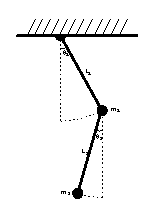
\includegraphics[width=.5\linewidth]{graphics/double_pendulum.eps}
	\caption{Illustration of the simple double pendulum.}
	\label{fig:doublependulum}
\end{figure}

\mikkel{Maybe the illustration needs to be changed in order properly show the positive direction of $\theta_2$ }

Equations should be developed such that, given an initial state, the position and subsequent movement can be derived from them.
This can be achieved using the Euler-Lagrange differential equations.
These will be found for this system throughout the remainder of this section.
Firstly, the position of the pendulums as a function of the angle must be determined.
The pendulums are placed in the x-y plane with the origin placed at the point of suspension of $p_1$.
When the pendulums are in the stable position, $\theta_1=\theta_2=0$, they are aligned with the y-axis.
The x-axis is positive to the right of the stable position.
The coordinates of $p_1=(x_1,y_1)$ and $p_2=(x_2,y_2)$ are as follows:
\begin{align}
	x_1 &= l_1\sin{\theta_1}\\
	y_1 &= -l_1\cos{\theta_1}\\
	x_2 &= l_1\sin{\theta_1} + l_2\sin{\theta_2}\\
	y_2 &= -l_1\cos{\theta_1} - l_2\cos{\theta_2}
\end{align}
While the derivatives are not used until later, they are presented here for clarity:
\begin{align}
	\dot{x}_1 &= l_1\cos{\theta}_1\dot{\theta}_1\\
	\dot{y}_1 &= l_1\sin{\theta}_1\dot{\theta}_1\\
	\dot{x}_2 &= l_1\cos{\theta}_1\dot{\theta}_1 + l_2\cos{\theta_2}\dot{\theta}_2\\
	\dot{y}_2 &= l_1\sin{\theta}_1\dot{\theta}_1 + l_2\sin{\theta_2}\dot{\theta}_2
\end{align}
In order to calculate the Euler-Lagrange diff. eq. it is necessary to first determine the lagrangian, $\mathcal{l}$:
\begin{equation}
	\mathcal{L}=E_k-E_p
\end{equation}
Where $E_k$ is the kinetic energy of the system and $E_p$, the potential energy.
The derivation of $E_p$:
\mikkel{g being the standard acceleration due to gravity}
\begin{align}
	E_p &= m_1 g y_1 + m_2 g y_2\\
		&= -m_1 g l_1 \cos{\theta_1} - m_2 g l_1 \cos{\theta_1} - m_2 g l_2 \cos{\theta_2}\\
		&= -(m_1+m_2)l_1g \cos{\theta_1}-m_2 g l_2 \cos{\theta_2}
		\label{eq:ep}
\end{align}
The derivation of $E_k$:
\begin{equation}
	\label{eq:ek}
	E_k = \frac{1}{2}m_1v_1^2+\frac{1}{2}m_2v_2^2
\end{equation}
As movement is present along both axes, the total velocity of either pendulum can be found as the derivative of the position and Pythagoras:
\begin{align}
	v_1^2 &= \dot{x}_1^2+\dot{y}_1^2\\
		&= l_1^2\dot{\theta}_1^2\cos{\theta}_1^2+l_1^2\dot{\theta}_1^2\sin{\theta_1}^2\\
		&= (\cos{\theta_1}^2+\sin{\theta_1}^2)l_1^2\dot{\theta}_1
\end{align}
Using the Pythagorean identity:
\begin{equation}
	\label{eq:v1}
	v_1^2 = l_1^2\dot{\theta}_1^2
\end{equation}
Similarly:
\begin{align}
	v_2^2 &= \dot{x}_2^2+\dot{y}_2^2\\
	&= (l_1\cos{\theta}_1\dot{\theta}_1 + l_2\cos{\theta_2}\dot{\theta}_2)^2+(l_1\sin{\theta}_1\dot{\theta}_1 + l_2\sin{\theta_2}\dot{\theta}_2)^2\\
	\begin{split}
		&= l_1^2\dot\theta_1^2\cos{\theta_1}^2+l_2^2\dot\theta_2^2\cos{\theta_2}^2+2l_1l_2\dot\theta_1\dot\theta_2\cos{\theta_1}\cos{\theta_2}\\
		&\qquad +l_1^2\dot\theta_1^2\sin{\theta_1}^2+l_2^2\dot\theta_2\sin{\theta_2}+2l_1l_2\dot\theta_1\dot\theta_2\sin{\theta_1}\sin{\theta_2}
	\end{split}
\end{align}
Isolating cosine and sine from the terms pairwise, 1 and 4, 2 and 5, 3 and 6, yields:
\mikkel{from equation 20? add in text}
\begin{align}
	\begin{split}
		v_2^2&=(\cos{\theta_1}^2+\sin{\theta_1}^2)l_1^2\dot\theta_1^2+(\cos{\theta_2}^2+\sin{\theta_2}^2)l_2^2\dot\theta_2^2\\
	&\qquad+(\cos{\theta_1}\cos{\theta_2}+\sin{\theta_1}\sin{\theta_2})2l_1l_2\dot\theta_1\dot\theta_2
	\end{split}
\end{align}
By applying the trigonimetric identities:
\begin{align}
	1&=\sin{\alpha^2}+\cos{\beta^2}\\
	\cos{(\alpha\pm\beta)}&=\cos\alpha\cos\beta\mp\sin\alpha\sin\beta
\end{align}
The result is found:
\begin{equation}
	\label{eq:v2}
	v_2^2=l_1^2\dot\theta_1^2+l_2^2\dot\theta_2^2+2l_1l_2\dot\theta_1^2\dot\theta_2^2\cos{(\theta_1-\theta_2)}
\end{equation}
Using equations \ref{eq:ep}, \ref{eq:ek}, \ref{eq:v1} and \ref{eq:v2} the lagrangian can be constructed:
\begin{align}
	\begin{split}
		\mathcal{L}&=\frac{1}{2}m_1l_1^2\dot\theta_1^2+\frac{1}{2}m_2\left(l_1^2\dot\theta_1^2+l_2^2\dot\theta_2^2+2l_1l_2\dot\theta_1^2\dot\theta_2^2\cos{(\theta_1-\theta_2)}\right)\\
		&\qquad+(m_1+m_2)l_1g\cos{\theta_1}+m_2l_2g\cos{\theta_2}
	\end{split}\\
	\begin{split}
		&=\frac{m_1l_1^2\dot\theta_1^2}{2}+\frac{m_2l_1^2\dot\theta_1^2}{2}+\frac{m_2l_2^2\dot\theta_2^2}{2}+l_1l_2\dot\theta_1\dot\theta_2\cos{(\theta_1-\theta_2)}\\
		&\qquad+(m_1+m_2)l_1g\cos{\theta_1}+m_2l_2g\cos{\theta_2}
	\end{split}
\end{align}
Which simplifies to:
\begin{equation}
	\label{eq:lagrangian}
	\begin{split}
		\mathcal{L}=\frac{(m_1+m_2)l_1^2\dot\theta_1^2}{2}+\frac{m_2l_2^2\dot\theta_2}{2}+l_1l_2\dot\theta_1\dot\theta_2\cos{(\theta_1-\theta_2)}\\
		+(m_1+m_2)l_1g\cos{\theta_1}+m_2l_2g\cos{\theta_2}\\
	\end{split}
\end{equation}
The Euler-Lagrange diff. eq. are defined as:
\begin{equation}
	\frac{d}{dt}\left(\frac{\partial \mathcal{L}}{\partial \dot\theta}\right)-\frac{\partial \mathcal{L}}{\partial \theta} = 0
\end{equation}
The three terms $\frac{\partial \mathcal{L}}{\partial \dot\theta}$,$\frac{d}{dt}\left(\frac{\partial \mathcal{L}}{\partial \dot\theta}\right)$ and $\frac{\partial l}{\partial \theta}$ are calculated next for each of the pendulums. 
\\For $p_1$:
\begin{align}
	\frac{\partial \mathcal{L}}{\partial \dot\theta_1}&=(m_1+m_2)l_1^2\dot\theta_1+m_2l_1l_2\dot\theta_2\cos{(\theta_1-\theta_2)}\\
	\begin{split}
		\frac{d}{dt}\left(\frac{\partial \mathcal{L}}{\partial \dot\theta_1}\right)&=(m_1+m_2)l_1^2\ddot\theta_1+m_2l_1l_2\ddot\theta_2\cos{(\theta_1-\theta_2)}\\
		&\qquad-m_2l_1l_2\dot\theta_2\sin{(\theta_1-\theta_2)(\dot\theta_1-\dot\theta_2)}
	\end{split}\\
	\frac{\partial \mathcal{L}}{\partial \theta_1} &= -m_2l_1l_2\dot\theta_1\dot\theta_2\sin(\theta_1-\theta_2)-(m_1+m_2)l_1g\sin{\theta_1}\\
\end{align}
\mikkel{Entering the x,x,x equations yields the first the Euler-Lagrange diff bla bla.}
\begin{align}
	\begin{split}
		0&=(m_1+m_2)l_1\ddot\theta_1+m_2l_2\ddot\theta_2\cos{(\theta_1-\theta_2)}\\
		&\qquad+m_2l_2\dot\theta_2^2\sin{(\theta_1-\theta_2)}+(m_1+m_2)g\sin{\theta_1}
	\end{split}
\end{align}
And $p_2$:

\begin{align}
	\frac{\partial \mathcal{L}}{\partial \dot\theta_2}&=m_2l_2^2\dot\theta_2+m_2l_1l_2\dot\theta_1\cos{(\theta_1-\theta_2)}\\
	\begin{split}
		\frac{d}{dt}\left(\frac{\partial \mathcal{L}}{\partial \dot\theta_2}\right)&=m_2l_2^2\ddot\theta_2+m_2l_1l_2\ddot\theta_1\cos{(\theta_1-\theta_2)}\\
		&\qquad -m_2l_1l_2\dot\theta_1\sin{(\theta_1-\theta_2)}(\dot\theta_1-\dot\theta_2)
	\end{split}\\
	\frac{\partial \mathcal{L}}{\partial \theta_2} &=m_2l_1l_2\dot\theta_1\dot\theta_2\sin{(\theta_1-\theta_2)}-m_2l_2g\sin{\theta_2}\\
	\label{eq:part}
\end{align}
\mikkel{Entering the x,x,x equations yields the second the Euler-Lagrange diff bla bla.}
\begin{align}
	\begin{split}
		0&=m_2l_2\ddot\theta_2+m_2l_1\ddot\theta_1\cos{(\theta_1-\theta_2)}\\
		&\qquad-m_2l_1\dot\theta_1^2\sin{(\theta_1-\theta_2)}+m_2g\sin{\theta_2}
	\end{split}
\end{align}
\thomas{eq. \ref{eq:part} has a minus in front of the first term according to our calculations. Determine why.}
% subsection simple_double_pendulum (end)

% section model_development (end)

\newpage
%!TEX root = ../main.tex
\section{The Platform} % (fold)
\label{sec:the_platform}
A new platform was made available to the project which fulfilled many of the requirements set by the application.
It consists of a cart, driven by a timing belt, mounted on an aluminium rail.
An image of the platform can be seen in figure \ref{fig:platform}.
\mikkel{Maybe mention what it was used for before?}
\begin{figure}[H]
 	\centering
 	\missingfigure{Image of the platform}
 	%\includegraphics[width=\linewidth]{graphics/platform}
 	\caption{The platform used in the project.}
 	\label{fig:platform}
 \end{figure} 
% section the_platform (end)
%!TEX root = ../main.tex
\section{Preliminary Testing} % (fold)
\label{sec:preliminary_testing}
In an effort to split the development into smaller, more managable parts, it was decided to initially develop the system such that it fulfills the following requirements:

\begin{itemize}
	\item The cart should be able to move with known position.
	\item Endstops on the platform should stop movement.
	\item Emergency button should stop movent.
\end{itemize}

Clearly, making the cart move is crucial in the development of the system and forms the basis for any later developments.
The latter two requirements are related to the safe operation of the platform.
It is expected that at least during development, an error may occur that causes the cart to move uncontrollably.
In such a situation the programmer should be able to completely shut off power to the motor.
The endstops will ensure that a minimum of mechanical or electrical damage is incurred on the platform in case of a cart crash.
The following paragraphs will explore what is required in order to fulfill the above requirements.
\subsection{Safety Circuitry} % (fold)
\label{sub:safety_circuitry}
Safety first.
A safety system should, whenever possible, be isolated from the remaining system.
That is, it should depend on non of the remaining circuitry or programming.
Usually, if it can at all be avoided, no programming should be involved in determining a safety condition.
With this in mind, the safety system for this platform should be designed in such a way that, when activated, it will cut power to the motors.
In order to more easily identify the cause of the fault, the remaining electronics should remain operational to maintain the current program status.
\\~\\
Creating the endstops can be done in a multitude of ways.
In this project three approaches were considered:
\paragraph{Mechanical Switch:} % (fold)
\label{par:mechanical_switch}
The simplest form of switch is the mechanical switch.
The switch should be mounted in such a way that the cart would move into the switch, therefore activating it.
This approach is not without issues.
Firstly, the simplest mounting solution would require the switch to be mounted in the direct path of the cart.
If the cart is traveling at full speed it is unlikely that the cart would stop before crashing into the switching mechanism, potentially damaging it.
A switch mounted in this fashion would need to be rather robust.
Some other mounting solutions could be thought of that do not suffer from this problem, especially if a flexible microswitch is used.
These types of switches can be fragile and may not be sufficiently durable, considering the usecase.
All mechanical switches have one drawback in common: they are mechanical.
Generally, mechanical items wear out over time and require maintainance or replacement.
% paragraph mechanical_switch (end)
\paragraph{Hall Effect Sensor:} % (fold)
\label{par:hall_effect_sensor}
This type of sensor measures magnetic fields and produces a voltage proportional to the strength of the field.
By placing a small neodymium magnet on the cart and mounting a hall effect sensor on the rail in such a way that the coincide would allow for detecting when the cart is above the sensor.
If the sensor is combined with a schmitt-trigger circuit the output could be a binary result, either the endstop is reached or it is not.
Using this method requires that a magnet is placed on the cart itself and that a sensor is mounted to the rail.
It should be noted that accelerating rather strong magnetic fields back and forth on the platform may not be the least electrically noisy solution one could think of.
Magnetic fields are also wide, meaning that the cart would "sneak up on" the threshold.
This requires some amount of calibration to determine the correct distance between sensor and magnet, which may not be mechanically simple to determine. 
% paragraph hall_effect_sensor (end)
\paragraph{Infrared Transceiver:} % (fold)
\label{par:infrared_transceiver}
This type of device is a combined LED and infrared sensor.
The LED is optimised for emitting infrared light, or radiation (IR), and the sensor for sensing it.
The LED emits IR outward from the device which, when an object is placed in front of it, will bounce off the object and be caught by the sensor.
As with the hall effect sensor, this type of device produces a voltage output proportional to the amount of IR being sensed and as such a schmitt-trigger circuit would also be benficial in this case.
With this sensor type it is important to realise that the LED will not be the only emitter of IR in the vicinity.
Any type of lamp will emit IR, especially glowbulbs (of which there are few left, luckily) but also sunlight contains some amount of IR.
When using this sensor the circuit should be designed in such a way that only the effect of the IR radiated back on the sensor will trigger the circuit.
The sensor should be mounted immediately below the cart so as to maximize the radiated IR and therefore the signal strength.
% paragraph infrared_transceiver (end)
\\~\\
While all of the above have their drawbacks, it was decided to use the infrared transceiver.
This sensor allows the greatest reliability while being reasonably simple to mount on the platform in that it requires no modification to the cart.
\\~\\
In addition to the endstops, also an emergency button, preferably red, should be able to cut power to the motors.
It may be that additional safety features are added later.
In order to minimize the amount of circuitry, all safety features will trip the same circuit.
\thomas{Add circuit showing the safety relay}
On figure \ref{fig:relay_circuit} is shown the safety circuitry.
A relay is mounted in series with the supply rail for the motor.
The default state for this relay should be \texttt{off}.
Then, in order to switch the system to the \texttt{on} state, the relay should be closed.
Should power to the relay coil ever fail i.e. something in the system has broken, power to the motor is cut off.
Since the relay is in series with the motor, it should also be capable of carrying the full design current, 80A.
One relay that fulfills these requirements is the.
\\~\\
The driver circuit for the relay is activated only when all safety conditions are off.
If at any point any of the safety conditions are tripped, the driver circuit shuts down, releasing the relay and turning off power to the motor.
Designing the safety circuit in this manner ensures that the system cannot be started or will shut down if any wires or components in the safety circuit break.

% subsection safety_circuitry (end)
\subsection{Power Board} % (fold)
\label{sub:power_board}
it is necessary to device some form of driving circuitry for the motor driving the timing belt.
On the platform is a Maxon 148867 Brushed DC Motor.
This is a 150W motor with a nominal current of 6A and a stall current of 80A.
Clearly, the system should under normal use not come anywhere close to stalling the motor but considering the use case, experimentation with control from students, it may be beneficial to design the circuitry such that it can withstand being stalled, for at least a short period of time.
In order to reach this goal, it is necessary to size the components for at least some amount above 80A continuous.
The \texttt{IPP045N10N3} MOSFET \cite{mosfet} is a 100V/100A MOSFET.
It is made in the standard TO-220 housing.
This housing allows for easy mounting of a heatsink and due to its wide application, there are many shapes and sizes to choose from.
Table \ref{tab:mosfetparameters} holds a list of the relevant parameters.

\begin{table}[tb]
	\centering
	\begin{tabular}{|r|c|c|c|}
	\hline
		\textbf{Parameter} & \textbf{Min} & \textbf{Typ} & \textbf{Max} \\
	\hline
		$V_{\text{th}}$ [V] & 2 & 2.7 & 3.5 \\
	\hline
		$R_{\text{ds(on)}}$ [m$\Omega$]& - & 3.6 & 4.2 \\
	\hline
		$Q_\text{g}$ [nC] & - & 88 & 117 \\
	\hline
		$I_\text{d}$ [A] & - & 100 & - \\
	\hline
		$V_{\text{ds}}$ [V] & 100 & - & - \\
	\hline
	\end{tabular}
	\caption{Relevant parameters of the IPP045N10N3 MOSFET \cite{mosfet} chosen for the full-bridge.
	Here, \vth is the gate threshold voltage, \ron is the drain-source on resistance, \qg is the total gate charge, \id is the maximum continuous drain current and \vds is the minimum guaranteed drain-source breakdown voltage.}
	\label{tab:mosfetparameters}
\end{table}

It should be noted that even though \vth is maximum 3.5V, this is not enough to fully open the MOSFET.
Rather, this voltage is where the MOSFET will start to conduct.
Figure \ref{fig:mosfettransfercharacteristic} reveals that the MOSFET is not fully conducting until \vgs $>4.5$V.

\begin{figure}[H]
	\centering
	\includegraphics[width=.5\linewidth]{graphics/mosfet_transfer_characteristic}
	\caption{Transfer characteristic of the IPP045N10N3 as per the datasheet.
	Inspecting the graph reveals that the maximum \id of 100A is reached at \vgs$\approx4.5\rightarrow4.75$V.}
	\label{fig:mosfettransfercharacteristic}
\end{figure}

The motor should be able to move in both directions so an h-bridge, or full-bridge is required.
By properly switching the MOSFETs in the circuit on and off the average voltage across the motor can be controlled and therefore also the speed and direction of the motor, see \ref{sec:hbridge} for more details.
\\~\\
\thomas{Insert reference to note on full-bridge drive}
Having chosen a MOSFET for the full-bridge, some form of driver must be designed for the full-bridge.
For this task, ready-made full-bridge drivers exist on the market that incorporate all of the electronics required to generate the driving signals, requiring only a PWM signal from the designer.
In order to choose one, a few parameters must be fulfilled.

\begin{itemize}
	\item \textbf{Output Current:} The amount of current necessary to properly drive the MOSFET.
	This value depends on the switching frequency of the application, the gate-to-source voltage ($V_{gs}$) and the total gate charge of the MOSFET.
	\item \textbf{Driving Voltage:} In order to ensure that the MOSFET is turned on quickly and fully the driver should be able to supply a voltage well above the gate threshold of the MOSFET.
	\item \textbf{High-Side Drive Capabilities:} The high side MOSFET of the full-bridge is referenced not to ground, but to $V_{\text{cc}}$.
	This means that in order to switch on this MOSFET $V_{\text{gs}}$ must be at least $V_{\text{cc}}+V_{\text{th}}$ where $V_{\text{th}}$ is the gate threshold voltage of the MOSFET.
	This is bootstrapping and is explained in more detail in section \ref{sec:bootstrap}.
	\item \textbf{Shoot-Through Protection and Deadtime:} Due to the structure of the full-bridge it is important that two MOSFETs on the same half-bridge are never on at the same time as this would result in a short from $V_{\text{cc}}$ to ground.
	This is resolved with a combination of deadtime (a delay where no MOSFET is on) and a logic table that ensures that an illegal switch combination can never happen.
\end{itemize}

The HIP4081AIBZ \cite{driver} full-bridge driver meets all of the above requirements.
It can supply up to 2.5A on the output pins with a voltage approximately 1V below \vcc, well above the required \vth.
Since the motor should, preferably, be driven outside the audible frequency range, it was chosen to set the switching frequency at 22kHz.
This frequency was chosen over an even higher frequency because increasing the frequency also increases the switching losses.
At this frequency there is $\frac{1}{22000}\approx45\mu$S per cycle. 
Well within this time the gate should be fully opened.
Since:

\begin{equation}
	I = C\frac{\text{dv}}{\text{dt}} \quad\Rightarrow\quad \text{dt} = C\frac{\text{dv}}{I}
\end{equation}
\thomas{Is this the correct way of calculating it?}

Accounting for various voltage drops it is assumed that \vgs is 10V, a rough estimate of the time to open the gate completely can be found as:

\begin{equation}
	\text{dt} = 117\cdot10^{-9}\frac{10}{2.5}\approx0.47\mu\text{S}
\end{equation}

This time is approximately 100 times shorter than the allotted time frame.
The component also has floating drive circuitry, meaning that by referencing the high-side driver to source of the high-side MOSFET, the driver can be made to output a voltage higher than \vcc.
This does require a few external components for the bootstrapping.
The choice of these components and a more in depth explanation of the procedure is given in section \ref{ssub:bootstrap_circuit}.
Finally, the component has a user-programmable dead time and shoot-through protection. 

HIP4081AIBZ - Full-bridge driver - (ISL83202)

IPP045N10N3 - Mosfet

choice of VGS, 8V - show graph of transfer characteristics of mosfet, high due to uncertainty.
% subsection power_board (end)
% section preliminary_testing (end)

%!TEX root = ../main.tex
\section{Board Design} % (fold)
\label{sec:board_design}
Multiple electronics components are required to realise the double pendulum being developed throughout this report.
This section explores the design of those components and the communication between them.
Most of the circuitry is combined on a single PCB, the driver board, however some of the functionality is moved to smaller boards, local to the place where they are needed.\\

The components of the system are listed here:
\begin{itemize}
	\item Motor Encoder
	\item Joint Encoder
	\item End Stops
	\item Motor Driver
	\item Emergency Circuitry
	\item Relay Driver
	\item RF Transceiver
	\item MicroZed 
\end{itemize}
Many of these components require a number of subcomponents, which will be explored further in later sections.

\subsection{Voltage Rails} % (fold)
\label{sub:voltage_rails}
In the design of the board it is necessary to determine which voltage rails are required for the system to function.
The power delivery for the MicroZed was designed by the authors in an earlier project \cite{isaswarm} and will be reused with minor changes.
This power delivery system provides, amongst other voltages, the 3.3V rail, originally intended for powering the MicroZed IO banks only.
In this system however, the RF tranceiver is also powered from this rail.
As a result a review of the circuitry around the 3.3V rail is necessary to ensure that it can provide the required power.
The MicroZed power delivery system, the encoders of the system, the endstops and part of the emergency circuitry are all driven from a 5V rail.
The Motor Driver, the HIP4081 \cite{driver} and the relay driving circuitry is driven from a 12V rail.
Finally, the motor is driven from a 24V rail, which will also be the main supply for the system.
This rail is not crucial to the design of the board as it is provided by an external, mains connected power supply and will not be explored further in this section.\\
The current requirement for each of these rails are discussed in the following paragraphs

\paragraph{3.3V:} % (fold)
\label{par:3_3v}
As mentioned, this rail is intended for powering the MicroZed IO banks.
In the original design the LMR10510XMF DC/DC converter is used to provide the necessary power.
This chip is capable of supplying up to 1A.
Components exist in the same series which are pin compatible and are capable of supplying up to 2A.
The RF Transceiver used in this project, however, \ref{} requires only up to 15mA when receiving data.
Assuming that Avnet has already provided headroom for the IO bank supply and considering that this project makes little use of the IO on the Zynq-7000 chip, it is deemed unnecessary to upgrade this supply and the original design is used as is.
% paragraph 3_3v_ (end)

\paragraph{5V:} % (fold)
\label{par:5v}
This rail supplies, mainly, the MicroZed.
The authors previously found \cite{isaswarm} that the maximum expected current draw seen from the MicroZed is 1.85A at 5V.
In addition, in this design, the 5V rail also powers the encoders, endstops and emergency circuitry.
There are two types of encoders, the HEDS-5540 \cite{heds5540}, which requires a maximum of 85mA and a Rolin magnetic encoder, which requires a maximum of 25mA.\\
The endstops are realised using the TCST2103 infrared sensor \cite{tcst2103}.
The majority of the current supplied to this sensor is used to power the infrared LED present in the component.
This current is decided by the resistor put in series with the LED and is estimated to be around 50mA per LED for a total of 100mA.
Another 10mA is added to that figure due to the collector current possible on the transistor side.\\
Finally the emergency circuitry along with some other digital electronics are powered from the 5V rail.
As these are all digital IC's that operate on nothing but signals, their individual powers are negligible but a very conservative 25mA power budget is provided for all of the digital electronics on the 5V rail. This brings the total power budget for the 5V rail to $\approx$2.1A.
See table \ref{tab:5vpowerbudget} for a full overview.

\begin{table}
	\centering
	\begin{tabular}{l|r}
		 Component & Current [mA]\\
		 \hline
		 MicroZed & 1850\\
		 HEDS-5540 & 85\\
		 Rolin Enc. & 25\\
		 TCST2103 & 110\\
		 Digital & 25\\
		 \hline
		 Total & 2095
	\end{tabular}
	\caption{Power budget for the 5V rail}
	\label{tab:5vpowerbudget}
\end{table}

In \cite{isaswarm} the authors used a design in which the PTH08080 is used to generate a 5V rail.
Reusing this module will save on design time as well as the budget available to the project and as such is desirable.
This module however, is capable of supplying only 2A at 5V, slightly less than the value calculated in this section.
By far the largest contributor to the power budget is the MicroZed.
The calculation of the contribution from the MicroZed is done assuming 85\% utilisation of PL and a conservative 80\% efficiency of internal DC/DC converters.
Considering this, it is safe to assume that the real power draw from the MicroZed is significantly smaller than the calculated value and as a result it is chosen to reuse the PTH08080 despite of apparent shortcomings of the module.
% paragraph 5 (end)

\paragraph{12V:} % (fold)
\label{par:12v}
This rail powers the HIP4081 motor driver, the relay coils, the bootstrap circuitry and the 5V DC/DC converter.
The PTH08080 DC/DC converter has a maximum input voltage of 18V and must be powered from the 12V rail rather than the 24V rail.
The module can provide 2A at 5V and as such will require $\approx$0.85A from the 12V rail.\\
There are two relays in the design, a smaller relay for controlling the inrush current and the larger main supply relay.
Both of these require power to stay in the closed position.
The first, the G6B \cite{g6b}, requires 16.7mA while the former, the LEV100A4ANG \cite{lev100}, requires 461mA.\\
The motor driver of the system, the HIP4081 requires only 10mA.
As mentioned, the bootstrap circuitry is also powered from the 12V rail.
Rather than a steady supply, this circuitry requires a large peak current for short periods while charging in between switching.
For this reason the design choice here is to determine what is available and choose the component which yields the most headroom while still being economically feasible.
Amongst all of the components the total power budget for the 12V rail is $\approx$1340mA.
See table \ref{tab:12vpowerbudget} for a full overview.

\begin{table}
	\centering
	\begin{tabular}{l|r}
		 Component & Current [mA]\\
		 \hline
		 PTH08080 & 850\\
		 G6B & 16.7\\
		 LEV100A4ANG & 461\\
		 HIP4081 & 10\\
		 \hline
		 Total & 1337.7
	\end{tabular}
	\caption{Power budget for the 12V rail}
	\label{tab:12vpowerbudget}
\end{table}

The PTN78020 delivers 6A at 12V and is part of the same series as the PTH08080 described earlier.
This allows many of the same design procedures to be reused.
In addition, the 6A current limit leaves sufficient room for the current spikes expected from the bootstrap circuitry.
The bootstrap circuitry is modified slightly to accomodate the limited supply as described in section \ref{}
% paragraph 12v_ (end)

% subsection voltage_rails (end)

% section board_design (end)


\subsection{PTN78020H Circuit}
\mikkel{A wild subsection appears! (Should be moved to a section where it makes sense)}
\begin{figure}
	\centering
	\includegraphics[width=\linewidth]{graphics/}
	\caption{Caption here}
	\label{fig:figure1}
\end{figure}
The \texttt{PTN78020H} DC/DC converter is used to generate the 12V rail. 
The component requires input and output capacitors in order to function properly and a resistor is needed to set the wanted output voltage. 
According to the components datasheet \cite{PTN78020H}, a 1\% 383 k$\Omega$ is needed to generate an output voltage of 12V.
The datasheet furthermore specifies that ceramic capacitance of 18.8 $\mu$F is needed at the input. 
It was chosen to use two 0805 10 $\mu$F capacitors.
In order to ensure stability the \texttt{PTN78020H} needs an output capacitance of 330 $\mu$F.
The datasheet specifies that if the application has load transients additional capacitance should be added to improve the response of the regulator. 
It was therefore decided to add two 330 $\mu$F in parallel. 
Two 10 $\mu$F ceramic capacitors are placed at the output to further improve the transient response. 
\mikkel{Figure?}



\subsection{Current Measuring}
\mikkel{A wild subsection appears! (Should be moved to a section where it makes sense)}
While reading in the literature it was found that measuring the current through the motor is beneficial for controlling the pendulums.

Current measurements are generally done by either hall effect based sensors or shunt resistors. 
Hall effect based sensors are generally the expensive solution and measuring small currents can be problematic. 
Therefore it was chosen to use a shunt resistor.
The basic idea is to place a resistor with a very low resistance in series with the load which current should be measured. 
Measuring the motor current when using a H-bridge can be done in a various of ways.
The three main ones are high-side, in-line and low-side placement of the shunt resistor as shown in figure \ref{fig:shunt_measure_high_in_low}.

\begin{figure}[h]
	\centering
    %\includegraphics[width=0.5\linewidth]{graphics/shunt_sense_high_in_low}
	\caption{xxxx.}
	\label{fig:shunt_measure_high_in_low}
\end{figure}
\mikkel{Figure should be replaced by own illustration}

\cite{shunt_placement} and \cite{Current_Sense_Circuit_Collection} specifies the advantages and disadvantages of the three configurations. 
Based on that it was decided to use the low-side configuration as it has low common voltage, it only needs a single sided supply and bi-directional current measurement is not needed.


\subsubsection{Requirements for the Current Measuring Circuit}
The output of the current measuring circuit is an analogue signal that needs to be measured by the ADC of the Zynq chip.
According to the Zynqs ADC user guide \cite{zynq_adc}, the measurable input range is from 0V to 1V, but the maximum allowed input voltage is 1.9V according to \cite{adc_zynq_webanswer}.
The absolute maximum current through the motor is the stall current which is 80A, but the motor will run at well below this level in normal operation.
The normal operation currents are expected to be up to 30A???(needs explanation somewhere...).
It was therefore decided that the circuit  needs to be able to measure currents of at least up to 40A.
The resolution per Ampere is increased by decreasing the current range that can be measured,
If the current gets any higher the ADC input should not be harmed meaning that the input voltage should not exceed 1.9V.

\mikkel{Below should be formatted differently}
\textbf{Requirements for the circuit:}
\begin{itemize}
	\item ADC input voltage does not exceed 1.9V when motor is stalling.
	\item Measures currents up to 40A, at minimum.
\end{itemize}


\subsubsection{Designing the Current Measuring Circuit}
The requirements listed above can be realized in a number of ways by choosing resistance of the shunt resistor and gain of the current-sense amplifier.
It was chosen to use a 200 $\mu \Omega$ SMD shunt resistor, as it is was the smallest resistance available at the university's electronics supplier. 
Such a small resistance yields a minimal voltage drop and thus a minimal power consumption.
The \texttt{INA210AIDCKT} from Texas Instruments was chosen as the current-sense amplifier, because is has all the wanted features, has a gain of 100 and a very low offset allowing it to be used in applications where the maximum voltage drop across the shunt resistor is 10 mV full-scale \cite{INA210AIDCKT}.
Using these components the stalling current of 80A will result in input voltage to the ADC of 1.6 V as shown in \ref{eq:adc_input_voltage1} and \ref{eq:adc_input_voltage2}.

\begin{equation}
	V_{max,input} = G \cdot V_{shunt}
	\label{eq:adc_input_voltage1}
\end{equation}
\begin{equation}
	V_{max,input} = G \cdot R_{shunt} \cdot I_{stall} = 100 \cdot 200\cdot10^{-6} \cdot 80 = 1.6V
	\label{eq:adc_input_voltage2}
\end{equation}

The maximum current that can be measured is 50A as shown in \ref{eq:adc_input_voltage3}.

\begin{equation}
	I_{max, measurable} = \frac{V_{max, measurable}}{R_{shunt}\cdot G} = \frac{1}{100 \cdot 200\cdot10^{-6} } = 50A
	\label{eq:adc_input_voltage3}
\end{equation}

These results clearly shows that the design meets the requirements.

%!TEX root = ../main.tex
\section{Joint Development}
\label{sec:joint_development}


\subsection{Joint Microcontroller}
\label{sub:joint_microcontroller}


\mikkel{Not finished}
\begin{itemize}
	\item Low power
	\item Compact size
	\item Three interrupt pins
	\item Eight I/O pins in total 
	\item SPI interface
	\item Non volatile memory
	\item 3.3V/5V supply
\end{itemize}


\begin{table}
	\centering
	\begin{tabular}{l}
		 \textbf{Requirements:} \\ \hline
		 Low power \\ \hline
		 Compact size \\ \hline
		 Three interrupt pins \\ \hline
		 Eight I/O pins in total\\ \hline
		 SPI interface \\ \hline
		 Non volatile memory \\ \hline
		 3.3V/5V supply \\ \hline
	\end{tabular}
	\caption{Hmmm. Not satisfied with this.}
	\label{tab:joint_mic_rec}
\end{table}

We chose the the ATtiny84 - yay!


\subsection{Voltage Rails}
\label{sub:voltage_rail}
It is necessary to determine which voltage rails are needed for the components on the joint board to function.
The wireless module, \texttt{NRF24}, and the ATtiny84 can both be run at 3.3V, but the Rolin encoder needs 5V.
Clearly a 3.3V rail and a 5V rail is needed. 
The current consumption on both rails need to be determined in order to specify the requirements for the voltage regulators and the required size of the battery needed.
\mikkel{There should be a nice introduction to this section about the Joint in general... Battery and so on.}


\paragraph{3.3V:}
\label{par:3_3v}
The \texttt{NRF24} module has maximum supply current of 12.3mA \cite{NFR24L01} and the \texttt{ATtiny82} has a maximum of 9mA \cite{attiny84}.
This totals 21.3mA of current that the 3.3V rail needs to supply.

\paragraph{5V:}
\label{par:5v}
The only component drawing current from the 5V rail is the Rolin encoder which has a maximum supply current of 20mA \cite{RLBD01}.

\subsection{Power Consumption} 
\label{subsub:power_consumption}
The power consumption at each rail is calculated and 

\begin{table}
	\centering
	\begin{tabular}{l|r|r}
		 Voltage rail 	& Current [mA] 	& Power [mW]\\
		 \hline
		 3.3V 			& 21.3			&70.3		\\
		 5V  			& 20 			&100		\\
		 \hline
		 Total 			& 				&170.3		
	\end{tabular}
	\caption{Power usage on voltage rails and in total.}
	\label{tab:power_joint}
\end{table}

\subsection{Battery}
\label{subsub:battery}
The physical dimensions of the battery is constrained by the free space in the designed joint.
It needs to be able to fit in a cylinder with a diameter of 57mm and height of 9mm.
Furthermore needs to have enough capacity to power the circuit for a full workday of a student, which is estimated to be 10 hours.
\mikkel{10 hours workday?}

\paragraph{9V Battery}
Batteries in the standard 9V package can purchased with with enough capacity, but the physical size disqualifies it.

\paragraph{Button Cell Battery}
Button cell batteries does live up to the physical constraints, but does not have the wanted capacity. 
Several of them can be put in series, but they still does not yield the wanted capacity.

\paragraph{Li-Ion Battery}
Lithium-Ion batteries have a very high energy density and it should therefore be possible to find a battery that fit both the physical and capacity constrains.
WE FOUND ONE!!!!!
\clearpage
\newpage
\section*{References}
\printbibliography[heading=none, keyword={all}]
\section*{Datasheets}
\printbibliography[heading=none, keyword={data}]
\end{document}